% Options for packages loaded elsewhere
\PassOptionsToPackage{unicode}{hyperref}
\PassOptionsToPackage{hyphens}{url}
%
\documentclass[
  twoside]{book}
\usepackage{amsmath,amssymb}
\usepackage{setspace}
\usepackage{iftex}
\ifPDFTeX
  \usepackage[T1]{fontenc}
  \usepackage[utf8]{inputenc}
  \usepackage{textcomp} % provide euro and other symbols
\else % if luatex or xetex
  \usepackage{unicode-math} % this also loads fontspec
  \defaultfontfeatures{Scale=MatchLowercase}
  \defaultfontfeatures[\rmfamily]{Ligatures=TeX,Scale=1}
\fi
\usepackage{lmodern}
\ifPDFTeX\else
  % xetex/luatex font selection
\fi
% Use upquote if available, for straight quotes in verbatim environments
\IfFileExists{upquote.sty}{\usepackage{upquote}}{}
\IfFileExists{microtype.sty}{% use microtype if available
  \usepackage[]{microtype}
  \UseMicrotypeSet[protrusion]{basicmath} % disable protrusion for tt fonts
}{}
\makeatletter
\@ifundefined{KOMAClassName}{% if non-KOMA class
  \IfFileExists{parskip.sty}{%
    \usepackage{parskip}
  }{% else
    \setlength{\parindent}{0pt}
    \setlength{\parskip}{6pt plus 2pt minus 1pt}}
}{% if KOMA class
  \KOMAoptions{parskip=half}}
\makeatother
\usepackage{xcolor}
\usepackage{color}
\usepackage{fancyvrb}
\newcommand{\VerbBar}{|}
\newcommand{\VERB}{\Verb[commandchars=\\\{\}]}
\DefineVerbatimEnvironment{Highlighting}{Verbatim}{commandchars=\\\{\}}
% Add ',fontsize=\small' for more characters per line
\usepackage{framed}
\definecolor{shadecolor}{RGB}{248,248,248}
\newenvironment{Shaded}{\begin{snugshade}}{\end{snugshade}}
\newcommand{\AlertTok}[1]{\textcolor[rgb]{0.94,0.16,0.16}{#1}}
\newcommand{\AnnotationTok}[1]{\textcolor[rgb]{0.56,0.35,0.01}{\textbf{\textit{#1}}}}
\newcommand{\AttributeTok}[1]{\textcolor[rgb]{0.13,0.29,0.53}{#1}}
\newcommand{\BaseNTok}[1]{\textcolor[rgb]{0.00,0.00,0.81}{#1}}
\newcommand{\BuiltInTok}[1]{#1}
\newcommand{\CharTok}[1]{\textcolor[rgb]{0.31,0.60,0.02}{#1}}
\newcommand{\CommentTok}[1]{\textcolor[rgb]{0.56,0.35,0.01}{\textit{#1}}}
\newcommand{\CommentVarTok}[1]{\textcolor[rgb]{0.56,0.35,0.01}{\textbf{\textit{#1}}}}
\newcommand{\ConstantTok}[1]{\textcolor[rgb]{0.56,0.35,0.01}{#1}}
\newcommand{\ControlFlowTok}[1]{\textcolor[rgb]{0.13,0.29,0.53}{\textbf{#1}}}
\newcommand{\DataTypeTok}[1]{\textcolor[rgb]{0.13,0.29,0.53}{#1}}
\newcommand{\DecValTok}[1]{\textcolor[rgb]{0.00,0.00,0.81}{#1}}
\newcommand{\DocumentationTok}[1]{\textcolor[rgb]{0.56,0.35,0.01}{\textbf{\textit{#1}}}}
\newcommand{\ErrorTok}[1]{\textcolor[rgb]{0.64,0.00,0.00}{\textbf{#1}}}
\newcommand{\ExtensionTok}[1]{#1}
\newcommand{\FloatTok}[1]{\textcolor[rgb]{0.00,0.00,0.81}{#1}}
\newcommand{\FunctionTok}[1]{\textcolor[rgb]{0.13,0.29,0.53}{\textbf{#1}}}
\newcommand{\ImportTok}[1]{#1}
\newcommand{\InformationTok}[1]{\textcolor[rgb]{0.56,0.35,0.01}{\textbf{\textit{#1}}}}
\newcommand{\KeywordTok}[1]{\textcolor[rgb]{0.13,0.29,0.53}{\textbf{#1}}}
\newcommand{\NormalTok}[1]{#1}
\newcommand{\OperatorTok}[1]{\textcolor[rgb]{0.81,0.36,0.00}{\textbf{#1}}}
\newcommand{\OtherTok}[1]{\textcolor[rgb]{0.56,0.35,0.01}{#1}}
\newcommand{\PreprocessorTok}[1]{\textcolor[rgb]{0.56,0.35,0.01}{\textit{#1}}}
\newcommand{\RegionMarkerTok}[1]{#1}
\newcommand{\SpecialCharTok}[1]{\textcolor[rgb]{0.81,0.36,0.00}{\textbf{#1}}}
\newcommand{\SpecialStringTok}[1]{\textcolor[rgb]{0.31,0.60,0.02}{#1}}
\newcommand{\StringTok}[1]{\textcolor[rgb]{0.31,0.60,0.02}{#1}}
\newcommand{\VariableTok}[1]{\textcolor[rgb]{0.00,0.00,0.00}{#1}}
\newcommand{\VerbatimStringTok}[1]{\textcolor[rgb]{0.31,0.60,0.02}{#1}}
\newcommand{\WarningTok}[1]{\textcolor[rgb]{0.56,0.35,0.01}{\textbf{\textit{#1}}}}
\usepackage{longtable,booktabs,array}
\usepackage{calc} % for calculating minipage widths
% Correct order of tables after \paragraph or \subparagraph
\usepackage{etoolbox}
\makeatletter
\patchcmd\longtable{\par}{\if@noskipsec\mbox{}\fi\par}{}{}
\makeatother
% Allow footnotes in longtable head/foot
\IfFileExists{footnotehyper.sty}{\usepackage{footnotehyper}}{\usepackage{footnote}}
\makesavenoteenv{longtable}
\usepackage{graphicx}
\makeatletter
\def\maxwidth{\ifdim\Gin@nat@width>\linewidth\linewidth\else\Gin@nat@width\fi}
\def\maxheight{\ifdim\Gin@nat@height>\textheight\textheight\else\Gin@nat@height\fi}
\makeatother
% Scale images if necessary, so that they will not overflow the page
% margins by default, and it is still possible to overwrite the defaults
% using explicit options in \includegraphics[width, height, ...]{}
\setkeys{Gin}{width=\maxwidth,height=\maxheight,keepaspectratio}
% Set default figure placement to htbp
\makeatletter
\def\fps@figure{htbp}
\makeatother
\setlength{\emergencystretch}{3em} % prevent overfull lines
\providecommand{\tightlist}{%
  \setlength{\itemsep}{0pt}\setlength{\parskip}{0pt}}
\setcounter{secnumdepth}{5}
% 中文支持 - 使用 ctex 包提供更好的中文排版
\usepackage{ctex}

% 中文字体设置 - 提供多个选项,取消注释其中一个配置

% 选项1:思源宋体 + 思源黑体(现代、清晰的专业字体)
% \setCJKmainfont{Noto Serif CJK SC}[BoldFont={Noto Serif CJK SC Bold},ItalicFont={AR PL KaitiM GB}]
% \setCJKsansfont{Noto Sans CJK SC}
% \setCJKmonofont{Noto Sans Mono CJK SC}

% 选项2:文鼎字体系列(传统、优雅的中文字体)
%\setCJKmainfont{AR PL UMing CN}[BoldFont={AR PL UMing CN},ItalicFont={AR PL KaitiM GB}]
%\setCJKsansfont{AR PL SungtiL GB}
%\setCJKmonofont{Noto Sans Mono CJK SC}

% 选项3:系统默认字体(确保兼容性)
% \setCJKmainfont{}
% \setCJKsansfont{}
% \setCJKmonofont{}


% 英文字体设置
%\usepackage{fontspec}
%\setmainfont{DejaVu Serif}
%\setsansfont{DejaVu Sans}
%\setmonofont{DejaVu Sans Mono}

% 正文字体大小设置 - ctex 已处理中英文字体大小匹配

% 页面设置
\usepackage[top=2.5cm, bottom=2.5cm, left=3cm, right=3cm]{geometry}

% 行间距设置
\usepackage{setspace}
\onehalfspacing  % 1.5倍行间距

% 段落缩进设置
\usepackage{indentfirst}
\setlength{\parindent}{2em}  % 每段开头空两格

% 数学支持
\usepackage{amsmath,amssymb,amsthm}
\usepackage{bm}
\usepackage{booktabs}
\usepackage{longtable}
\makeatletter
\def\thm@space@setup{%
  \thm@preskip=8pt plus 2pt minus 4pt
  \thm@postskip=\thm@preskip
}
\makeatother


% 章节标题样式 - ctex 已提供优化的中文标题样式
% 如果需要自定义,可以取消注释以下设置:
% \usepackage{titlesec}
% \titleformat{\chapter}[display]
%   {\normalfont\Huge\bfseries\filcenter}{\chaptertitlename\ \thechapter}{20pt}{\Huge}
% \titleformat{\section}
%   {\normalfont\Large\bfseries}{\thesection}{1em}{}
% \titleformat{\subsection}
%   {\normalfont\large\bfseries}{\thesubsection}{1em}{}

% 图表标题 - ctex 已优化中文标题
\usepackage{caption}
\captionsetup{font=small,labelsep=quad}

% 超链接
\usepackage{hyperref}
\hypersetup{
  colorlinks=true,
  linkcolor=blue,
  filecolor=magenta,      
  urlcolor=cyan,
  pdftitle={生态统计学},
  pdfauthor={沈国春、李勤}
}

% 代码环境
\usepackage{listings}
\lstset{
  basicstyle=\footnotesize\ttfamily,  % 缩小代码字体
  breaklines=true,
  frame=single,
  numbers=left,
  numberstyle=\tiny,
  stepnumber=1,
  numbersep=5pt
}
\usepackage{booktabs}
\usepackage{longtable}
\usepackage{array}
\usepackage{multirow}
\usepackage{wrapfig}
\usepackage{float}
\usepackage{colortbl}
\usepackage{pdflscape}
\usepackage{tabu}
\usepackage{threeparttable}
\usepackage{threeparttablex}
\usepackage[normalem]{ulem}
\usepackage{makecell}
\usepackage{xcolor}
\ifLuaTeX
  \usepackage{selnolig}  % disable illegal ligatures
\fi
\usepackage[]{natbib}
\bibliographystyle{apalike}
\IfFileExists{bookmark.sty}{\usepackage{bookmark}}{\usepackage{hyperref}}
\IfFileExists{xurl.sty}{\usepackage{xurl}}{} % add URL line breaks if available
\urlstyle{same}
\hypersetup{
  pdftitle={生态统计学},
  pdfauthor={沈国春、李勤},
  hidelinks,
  pdfcreator={LaTeX via pandoc}}

\title{生态统计学}
\author{沈国春、李勤}
\date{2025-10-04}

\begin{document}
\maketitle

{
\setcounter{tocdepth}{1}
\tableofcontents
}
\listoffigures
\listoftables
\setstretch{1.5}
\hypertarget{ux524dux8a00}{%
\chapter*{前言}\label{ux524dux8a00}}
\addcontentsline{toc}{chapter}{前言}

\hypertarget{ux4e3aux4ec0ux4e48ux8981ux5b66ux751fux6001ux7edfux8ba1}{%
\section{为什么要学生态统计}\label{ux4e3aux4ec0ux4e48ux8981ux5b66ux751fux6001ux7edfux8ba1}}

\hypertarget{ux5728ux4e0dux786eux5b9aux7684ux4e16ux754cux4e2dux5bfbux627eux89c4ux5f8b}{%
\subsection{在不确定的世界中寻找规律}\label{ux5728ux4e0dux786eux5b9aux7684ux4e16ux754cux4e2dux5bfbux627eux89c4ux5f8b}}

当我们选择生态学,我们便选择拥抱一个充满动态、关联与不确定性的复杂世界。我们研究的对象------从一只蝴蝶的迁飞路径,到整个森林群落的演替进程------本质上都不是确定性的。我们无法像物理学家在理想真空中预测小球落地那样,精准断言明年这片湿地中将有多少只丹顶鹤诞生。这种不确定性并非生态学的缺陷,恰恰是其魅力与挑战的核心。而概率与统计,正是我们理解、量化和驾驭这种不确定性的\textbf{最强有力的语言和工具}。可以说,一位现代生态学专业人才若不能流利使用这种语言,便如同一位探险家没有地图与指南针,难以在数据的海洋与自然的混沌中寻得可靠的规律。

\textbf{首先,概率论为我们提供了描述和预测``不确定性''的语法。} 生态学系统是由无数随机事件交织构成的:一次授粉是否成功?一只幼崽能否躲过天敌?一场火灾何时发生?概率让我们能够衡量这些事件的可能性。当我们谈论一个物种的灭绝风险、一种疾病在种群中的传播速率,或是气候变化下物种分布范围的变迁时,我们口中的``风险''、``速率''和``趋势'',其内核都是概率。例如,在保护生物学中,我们使用种群生存力分析(PVA)来预测一个濒危种群未来的命运,这本质上就是一个复杂的概率模型,它综合考虑了出生率、死亡率、环境波动等随机因素。没有概率论,我们对未来的预测将只能是模糊的猜测,而非基于数据的科学评估。

\textbf{进而,描述统计赋予了我们将纷繁复杂的自然数据转化为清晰洞见的能力。} 野外调查归来,我们面对的可能是在数十个样方中记录的成千上万条关于物种、高度、密度、土壤参数的数据。这些原始数据本身如同一堆未经雕琢的玉石,价值隐藏于混乱之中。描述统计就是我们的雕刻刀:通过计算平均值,我们了解了群落的平均高度;通过标准差,我们知晓了树木胸径的变异程度;通过绘制直方图,我们直观地看到了种群年龄结构的分布模式------是健康的金字塔形还是衰退的倒金字塔形?箱线图可以瞬间比较出不同生境下鸟类体型的差异。这些工具帮助我们简化、组织和可视化数据,让我们能够``看见''数据背后的故事,从而提出更精准的科学问题。

\textbf{最终,推断统计完成了从``所见''到``所知''的惊险一跃,这是现代生态学研究的基石。} 生态学的根本困境在于,我们几乎永远无法普查整个种群或生态系统(总体)。我们所能做的,是在时间、经费和人力的限制下进行抽样调查------设置样方、布设红外相机、进行航线调查。那么,一个核心问题随之而来:我们如何能确信从这有限的样本中得出的结论,能够代表我们真正关心的总体?推断统计给出了答案。置信区间告诉我们,基于样本数据,我们对总体参数(如整个森林的生物量)的估计有多大的把握范围。假设检验则提供了一套严谨的``反证法''逻辑,帮助我们判断观察到的模式(如施肥区与对照区产量差异)究竟是真实的效应,还是仅仅由抽样偶然性造成的``假象''。当我们说``施肥显著提高了草地生产力''(p \textless{} 0.05)时,我们正是在运用统计语言,以极大的信心宣布这一发现并非偶然。这使得我们的工作从对特定样本的描述,上升到了对普遍规律的推论,赋予了生态学相关成果以普适性和说服力。

总而言之,概率与统计并非强加于生态学之上的数学枷锁,而是根植于生态学研究对象本质的内在需求。它们是我们将观察数据转化为可靠结论所不可或缺的桥梁。从准确评估一个生态系统的健康状况,到可信地预测环境变化的影响,每一步都深深依赖于概率与统计的思维框架。掌握这门语言,意味着你们将获得一种强大的能力:\textbf{在一片看似混沌的自然现象中,清晰地聆听出规律的低语,并基于数据做出科学的判断和决策。} 这不仅是一门必修课,更是你们未来职业生涯中,无论是在科研、保护、管理还是咨询领域,最忠实的伙伴和最可靠的向导。

\hypertarget{aiux65f6ux4ee3ux7684ux673aux9047ux4e0eux9677ux9631}{%
\subsection{AI时代的机遇与陷阱}\label{aiux65f6ux4ee3ux7684ux673aux9047ux4e0eux9677ux9631}}

生态学,这门诞生于野外观察与手绘记录的学科,正经历着一场由数据驱动的深刻革命。当我们研究的尺度从单个样方扩展到整个星球,当我们的数据从几十个手写记录点激增至TB级别的卫星遥感影像、声学监测数据和基因组序列时,传统的数据处理与分析方法已显得力不从心。毫无疑问,现代计算工具------从强大的统计软件(如R、Python)到高性能计算集群------已经成为生态从业者不可或缺的''数字望远镜''和''计算实验室''。它们让我们能够驾驭海量数据,构建复杂的模型,从而解析自然界中前所未有的复杂模式。然而,这场变革的最新篇章------人工智能(AI),特别是机器学习技术的融入,在将我们的分析能力推向新高度的同时,也正将生态学相关工作和研究引入一个机遇与风险并存的全新领域。

\textbf{首先,我们必须承认,现代化分析工具,尤其是AI,正以前所未有的方式赋能生态学相关工作。} 它们极大地提升了我们处理``大数据''的效率和深度。传统统计方法往往在应对高维度、非线性关系时捉襟见肘,而机器学习算法却能如鱼得水。例如,利用深度学习模型,我们可以自动识别数以百万计的红外相机照片中的物种,将研究人员从漫长枯燥的人工判读中解放出来;通过分析数十年的卫星图像,AI能精准刻画森林砍伐、城市扩张的动态,其速度和精度远超人工目视解译。更重要的是,AI具有强大的''模式发现''能力,它能在纷繁复杂的环境变量与物种分布数据中,挖掘出人类可能忽略的微妙关联,甚至为决策提供新的依据。这仿佛为我们提供了一种''超级直觉'',使得预测物种对气候变化的响应、解析生态系统韧性的临界点等复杂问题成为了可能。AI工具正变得越来越''平民化'',用户友好的界面和自动化流程降低了技术门槛,让更多生态从业者能够专注于实际问题本身,而非复杂的编程实现。

\textbf{然而,这把锋利的``双刃剑''的另一面,是潜藏的巨大风险,其核心在于``黑箱''效应与因果关系的混淆。} 许多最强大的机器学习模型(如深度神经网络)就像一个黑箱:我们输入数据,它给出精准的预测,但其内部的决策过程往往难以解释。对于生态从业者而言,知道''某种鸟类更可能出现在哪里''固然重要,但理解''为什么''------即其背后的生态学机制(是温度、食物来源还是栖息地结构?)------才是深入理解问题的关键。AI模型可能精准地预测了物种分布,但其建立的相关关系可能只是数据中的虚假模式,甚至可能指向一个荒谬的因果关系(例如,根据数据,它可能''发现''电价上涨是导致蛙类减少的主要原因,只因二者在时间序列上巧合地相关)。这种对相关性的过度依赖,而缺乏因果推断,可能导致我们得出错误的结论,甚至制定出无效或有害的决策和政策。

\textbf{此外,AI模型的性能高度依赖于训练数据的质量与代表性,这带来了``垃圾进,垃圾出''的经典困境。} 生态学数据往往存在样本偏差(例如,交通便利的地区观测记录多,偏远地区记录少)、系统误差和噪声。如果一个AI模型是用有偏差的数据训练出来的,那么它只会强化并放大这种偏差。例如,一个用于识别全球鸟类分布的模型,如果主要用北美和欧洲的数据训练,它在预测南美热带雨林物种时可能会表现极差。这不仅会导致分析错误,更会加剧数据应用的不平等,使得数据匮乏地区的生态问题被进一步忽视。更严峻的风险在于,从业者可能因为过度依赖AI输出的''权威''结果,而丧失了对数据本身的批判性审视和实地经验的直觉,最终导致生态学这门扎根于自然的学科,与其实践本体渐行渐远。

\textbf{因此,在AI时代,生态专业人才的角色非但没有被削弱,反而变得更加关键。} 我们绝不能沦为算法的仆从,而必须成为其智慧的驾驭者。未来的生态专业人才需要具备更全面的素养:一方面,要拥抱技术,学会与AI工具协同工作;另一方面,必须坚守科学精神,对模型结果保持深刻的怀疑和批判。我们需要不断追问:这个模型的假设是什么?训练数据是否有代表性?结果是否有实际意义?能否被独立的观察和实践所验证?

归根结底,现代化分析工具和AI是生态专业人才手中的超级''望远镜'',它让我们看得更远、更清,但望远镜本身并不能告诉我们星空的奥秘。真正的价值,依然依赖于望远镜背后那颗充满好奇心、严谨逻辑和深厚生态学知识的大脑。在这场方兴未艾的技术革命中,我们必须善用工具之力,同时时刻警惕其陷阱,确保技术最终服务于我们更深切地理解、保护和可持续利用这个脆弱星球的终极使命。

\hypertarget{ux672cux4e66ux4ecbux7ecd}{%
\section{本书介绍}\label{ux672cux4e66ux4ecbux7ecd}}

基于前文对生态学数据分析和AI时代挑战的深入探讨,本书旨在为生态学专业人才提供一套完整、实用的统计思维和数据分析能力培养体系。在数据驱动决策日益重要的今天,掌握统计方法不仅是科研工作的基础,更是生态保护、环境管理、政策制定等各个领域从业者的核心素养。

本书以R语言为主要工具,系统介绍生态学研究中常用的统计方法,特别强调统计思维在实际问题中的应用。我们相信,真正的数据分析能力不仅在于掌握技术工具,更在于培养对数据的批判性思维和对结果的科学解读能力。

本书特色:

\begin{itemize}
\tightlist
\item
  \textbf{问题导向}:从生态学实际问题出发,强调统计方法在真实场景中的应用价值
\item
  \textbf{实践性强}:基于R语言实现,提供大量可复现的代码示例和生态数据案例
\item
  \textbf{思维培养}:不仅教授技术,更注重统计思维和数据分析逻辑的培养
\item
  \textbf{循序渐进}:从基础概念到高级方法,构建完整的学习路径
\item
  \textbf{时代特色}:融入对AI时代数据分析新挑战的思考,培养批判性思维
\end{itemize}

本书使用以下R包:

\begin{Shaded}
\begin{Highlighting}[]
\FunctionTok{install.packages}\NormalTok{(}\FunctionTok{c}\NormalTok{(}
  \StringTok{"tidyverse"}\NormalTok{, }\StringTok{"vegan"}\NormalTok{, }\StringTok{"lme4"}\NormalTok{, }\StringTok{"ggplot2"}\NormalTok{,}
  \StringTok{"bookdown"}\NormalTok{, }\StringTok{"knitr"}\NormalTok{, }\StringTok{"rmarkdown"}\NormalTok{, }\StringTok{"DiagrammeR"}\NormalTok{,}
  \StringTok{"showtext"}\NormalTok{, }\StringTok{"gridExtra"}\NormalTok{, }\StringTok{"moments"}\NormalTok{,}
  \StringTok{"gganimate"}\NormalTok{, }\StringTok{"gapminder"}\NormalTok{, }\StringTok{"audio"}\NormalTok{, }\StringTok{"patchwork"}\NormalTok{,}
  \StringTok{"sn"}\NormalTok{, }\StringTok{"spdep"}\NormalTok{, }\StringTok{"reshape2"}\NormalTok{, }\StringTok{"ineq"}\NormalTok{, }\StringTok{"NetIndices"}\NormalTok{,}
  \StringTok{"vegan"}\NormalTok{, }\StringTok{"bipartite"}\NormalTok{, }\StringTok{"pwr"}\NormalTok{, }\StringTok{"marked"}\NormalTok{, }\StringTok{"Distance"}\NormalTok{,}
  \StringTok{"fitdistrplus"}\NormalTok{, }\StringTok{"brms"}\NormalTok{, }\StringTok{"ppcor"}\NormalTok{, }\StringTok{"energy"}\NormalTok{, }\StringTok{"infotheo"}\NormalTok{,}
  \StringTok{"tseries"}\NormalTok{, }\StringTok{"forecast"}\NormalTok{, }\StringTok{"gstat"}\NormalTok{, }\StringTok{"geoR"}\NormalTok{, }\StringTok{"automap"}\NormalTok{,}
  \StringTok{"ape"}\NormalTok{, }\StringTok{"phytools"}\NormalTok{, }\StringTok{"picante"}\NormalTok{, }\StringTok{"corrplot"}\NormalTok{, }\StringTok{"coin"}\NormalTok{,}
  \StringTok{"geiger"}\NormalTok{, }\StringTok{"spaa"}\NormalTok{, }\StringTok{"adespatial"}\NormalTok{, }\StringTok{"relaimpo"}\NormalTok{,}
  \StringTok{"MuMIn"}\NormalTok{, }\StringTok{"caret"}\NormalTok{, }\StringTok{"car"}\NormalTok{, }\StringTok{"BMS"}\NormalTok{, }\StringTok{"monomvn"}\NormalTok{, }\StringTok{"BayesFactor"}\NormalTok{,}
  \StringTok{"gratia"}\NormalTok{, }\StringTok{"AER"}\NormalTok{, }\StringTok{"lmerTest"}\NormalTok{, }\StringTok{"performance"}\NormalTok{,}
  \StringTok{"spatialreg"}\NormalTok{, }\StringTok{"spTimer"}\NormalTok{, }\StringTok{"lavaan"}\NormalTok{, }\StringTok{"semPlot"}\NormalTok{,}
  \StringTok{"rpart.plot"}\NormalTok{, }\StringTok{"pdp"}\NormalTok{, }\StringTok{"torch"}\NormalTok{, }\StringTok{"DHARMa"}
\NormalTok{))}

\NormalTok{devtools}\SpecialCharTok{::}\FunctionTok{install\_github}\NormalTok{(}\StringTok{"GotelliLab/EcoSimR"}\NormalTok{)}
\CommentTok{\#ubuntu sudo apt install r{-}cran{-}openmx}
\end{Highlighting}
\end{Shaded}

\hypertarget{ux8bfeux7a0bux5728ux7ebfux8d44ux6e90}{%
\section{课程在线资源}\label{ux8bfeux7a0bux5728ux7ebfux8d44ux6e90}}

课程简明手册

\begin{itemize}
\tightlist
\item
  网页版 \url{https://guochunshen.github.io/ecological-statistics}
\item
  PDF版 \url{https://gitee.com/gcshen/ecological-statistics/blob/master/docs/ecological-statistics.pdf}
\item
  原代码 \url{https://gitee.com/gcshen/ecological-statistics}
\end{itemize}

\hypertarget{ux5b66ux4e60ux65b9ux5f0f}{%
\section{学习方式}\label{ux5b66ux4e60ux65b9ux5f0f}}


\includegraphics{imgs/how to learn R.png}

\includegraphics{imgs/how to learn R 2.png}

\hypertarget{ux7edfux8ba1ux7f16ux7a0bux57faux7840}{%
\chapter{统计编程基础}\label{ux7edfux8ba1ux7f16ux7a0bux57faux7840}}

\hypertarget{ux5f15ux8a00}{%
\section{引言}\label{ux5f15ux8a00}}

在大语言模型(LLM)成为强大编程助手的今天,编程教育的重心正在发生根本性的转移。死记硬背语法和API细节的价值确实在大幅降低。这一变革标志着编程教育从''技能导向''向''思维导向''的深刻转型。过去,编程教学往往过分强调记忆各种语言的语法规则、函数库的API细节,以及特定框架的使用方法,学生需要花费大量时间在机械记忆上。然而,随着Deepseek等AI编程助手的普及,这些原本需要记忆的知识点现在可以通过简单的自然语言查询即时获得。这并不意味着编程变得不重要,恰恰相反,它意味着编程教育的价值需要重新定位。

在新的AI时代,编程教育的核心价值不再体现在''知道多少语法'',而是体现在''能够解决什么问题''和''如何设计分析方案''。学生需要培养的是更高层次的思维能力:如何将一个复杂的现实问题分解成可计算的分析步骤,如何选择合适的统计方法和数据处理技术,如何设计清晰的分析流程,如何与AI进行有效协作以验证和优化分析结果。这些能力构成了AI时代统计编程人员的核心竞争力。

具体而言,统计编程教育应该着重培养以下几个关键能力:首先是问题分解与抽象建模能力,这要求学生能够将复杂的统计问题转化为可计算的数学模型;其次是算法思维,理解不同统计方法的计算原理和适用条件;再次是数据处理能力,从数据收集、清洗到分析的完整流程设计;最后是与AI协作的能力,包括精准提问、代码审查和迭代优化。这些能力的培养需要项目驱动的教学方法,让学生在解决真实统计问题的过程中逐步建立编程思维框架。

对于生态学专业的你来说,理解全球AI竞争中的算法核心地位,就如同理解生态系统中的关键物种------它虽不直接可见,却足以重塑整个环境格局。DeepSeek作为中国AI企业,正是凭借算法的突破性创新,改写了全球AI产业长期以来依赖``堆算力''的发展路径。它通过自研的混合专家模型(MoE)架构和最新的DeepSeek稀疏注意力(DSA) 等算法,在保证模型高性能的同时,大幅提升了训练和推理效率,并将API成本降低了超过50\%。这种``效能革命''证明了高效的算法设计本身可以成为一种强大的竞争力,打破了由算力规模构筑的壁垒。

这种教育重心的转移对学生提出了新的要求,也带来了新的机遇。学生不再需要为记忆琐碎的语法细节而苦恼,可以将更多精力投入到统计建模和数据分析中。教师的教学方法也需要相应调整,从传统的''语法讲解+练习题''模式转向''数据分析项目实践+统计思维训练''模式。通过这种转变,统计编程教育将更好地服务于培养学生的数据科学思维和统计分析能力这一根本目标,为他们在AI时代的科研和数据分析工作奠定坚实基础。

现在,对学生来说,最重要的不再是''如何写代码'',而是''解决什么问题''和''为何这样解决''。

本章将介绍AI时代的编程思维框架,帮助学生培养与LLM协同工作的核心能力,并通过R语言实践掌握现代数据分析方法。

\hypertarget{ux6838ux5fc3ux80fdux529bux57f9ux517bux6846ux67b6}{%
\section{核心能力培养框架}\label{ux6838ux5fc3ux80fdux529bux57f9ux517bux6846ux67b6}}

以下是学生在学习编程课程时最需要培养的核心技能,我将其分为三大类:

\hypertarget{ux9ad8ux9636ux601dux7ef4ux4e0eux95eeux9898ux89e3ux51b3ux80fdux529b}{%
\subsection{高阶思维与问题解决能力}\label{ux9ad8ux9636ux601dux7ef4ux4e0eux95eeux9898ux89e3ux51b3ux80fdux529b}}

最核心、最根本的能力是驾驭LLM的''方向盘''能力。在AI时代,数据分析师不再需要记忆繁琐的编程语法细节,但必须具备更高层次的思维框架来指导AI工具完成复杂的数据分析任务。这种高阶思维框架主要包括三个方面:首先是问题分解与抽象建模能力,即将复杂的生态学问题转化为清晰可执行的分析流程;其次是算法与数据结构思维,即对计算效率和数据处理优化的深刻理解;最后是数据分析流程设计与规划能力,即从宏观视角系统性地设计整个数据分析生命周期的能力。这三种能力共同构成了AI时代生态学数据分析师的核心竞争力,确保研究者能够站在战略高度设计分析方案,而不仅仅是执行具体的编程任务。

\hypertarget{ux95eeux9898ux5206ux89e3ux4e0eux62bdux8c61ux5efaux6a21ux80fdux529b}{%
\subsubsection{问题分解与抽象建模能力}\label{ux95eeux9898ux5206ux89e3ux4e0eux62bdux8c61ux5efaux6a21ux80fdux529b}}

问题分解与抽象建模能力是指将一个复杂的、模糊的现实世界问题,分解成一个个清晰的、可执行的分析步骤的能力。这种能力不仅涉及技术层面的分解,更包含对问题本质的深刻理解和抽象思维。在生态学研究中,这意味着能够将复杂的生态系统现象转化为可计算、可分析的统计模型和分析流程。

这种能力的重要性在于,虽然LLM可以帮你写数据处理代码,但它无法替你决定''整个分析流程应该分成哪几个关键步骤''或''这个统计问题应该采用哪种分析方法''。这是人类分析师最核心的价值。在AI时代,这种能力变得更加关键,因为LLM擅长执行具体任务,但缺乏对复杂研究问题的整体把握和统计规划能力。学生需要学会如何将模糊的研究问题转化为清晰的分析需求,这样才能有效指导LLM完成具体实现。

在生态学实践中,问题分解能力体现在具体的研究场景中。例如,分析森林生态系统的物种多样性变化,需要分解为数据收集、数据清洗、多样性指数计算、统计分析、结果可视化等步骤。具体而言,这个过程可以进一步细化为:首先确定研究目标和数据需求,包括样地选择标准、调查方法和数据格式;然后设计数据收集方案,考虑野外调查的可行性和数据质量控制;接着制定数据清洗流程,处理缺失值、异常值和数据标准化问题;再选择合适的多样性指数计算方法,如Shannon-Wiener指数、Simpson指数等,并考虑其生态学意义;最后设计统计分析框架和可视化方案,确保结果能够清晰反映生态学规律。

这种问题分解能力在生态学研究中尤为重要,因为生态系统的复杂性往往超出直觉理解。通过系统性的分解和抽象,研究者能够将看似混沌的自然现象转化为有序的分析流程。例如,在研究气候变化对物种分布的影响时,需要将问题分解为气候数据获取、物种分布数据整合、生态位模型构建、未来情景预测等多个分析环节,每个环节都有其特定的技术要求和生态学考量。

培养这种能力的关键在于实践和反思。学生应该通过具体的生态学项目,学习如何识别问题的核心要素,如何设计合理的分析流程,以及如何在技术实现和生态学意义之间找到平衡。随着经验的积累,这种问题分解和抽象建模能力将成为学生在AI时代进行生态学研究的核心竞争力。

\hypertarget{ux7b97ux6cd5ux4e0eux6570ux636eux7ed3ux6784ux601dux7ef4}{%
\subsubsection{算法与数据结构思维}\label{ux7b97ux6cd5ux4e0eux6570ux636eux7ed3ux6784ux601dux7ef4}}

算法与数据结构思维是数据分析师的核心能力之一,它不仅仅是理解不同算法和数据结构的适用场景,更重要的是培养一种''计算效率意识''。这种思维要求我们理解不同统计方法的时间/空间复杂度(Big O Notation),知道在什么情况下应该选择哈希表而不是数组来快速查找数据,何时应该采用动态规划而不是暴力破解来处理复杂的优化问题。在生态学数据分析中,这种思维体现在对数据处理流程的优化意识上------比如知道在什么情况下应该使用向量化操作而不是循环,何时应该对数据进行预处理以提高后续分析的效率。这种思维还延伸到对统计方法计算复杂度的理解,比如知道某些复杂的生态位模型可能需要数小时甚至数天才能完成计算,而简单的线性回归可能只需要几秒钟。

在AI时代,LLM可以根据你的要求实现一个统计函数,但你必须具备足够的专业知识来告诉它具体需要什么。比如,你不能简单地说''帮我做个t检验'',而应该明确说明''我需要一个能够处理缺失值、输出置信区间、并且可以进行方差齐性检验的t检验函数''。这种精确的需求描述能力来自于对统计方法内在逻辑的深刻理解。更重要的是,当LLM给出解决方案时,你需要具备评判能力------这个方案真的最优吗?有没有考虑边界情况?这个统计方法是否适用于我的数据类型?比如,LLM可能会推荐使用Pearson相关系数来分析你的数据,但如果你知道自己的数据不符合正态分布,就应该选择Spearman或Kendall相关系数。这种批判性思维是AI难以替代的,它确保了分析结果的科学性和可靠性。

处理大规模的物种分布数据时,算法与数据结构思维显得尤为重要。假设你正在分析全国范围的鸟类分布数据,包含数百万条观测记录。如果你简单地使用线性搜索来查找特定物种的记录,可能需要数小时才能完成。但如果你具备数据结构思维,就会想到使用哈希表或数据库索引来建立快速查找机制,将查询时间从小时级降低到秒级。另一个例子是生态位模型的构建:如果你要使用MaxEnt模型分析某个濒危物种的分布规律,需要理解这个算法的计算复杂度,知道在什么情况下应该对数据进行降采样,什么情况下可以使用并行计算来加速模型训练。在处理时间序列的生态监测数据时,你需要知道何时应该使用滑动窗口分析而不是对整个数据集进行全局分析。这种思维还体现在对数据存储格式的选择上------知道在什么情况下应该使用CSV格式便于人工查看,什么情况下应该使用Parquet或Feather格式来提高读写效率。通过培养这种算法与数据结构思维,生态学研究者能够在面对海量生态数据时做出明智的技术决策,确保分析工作既高效又准确。

\hypertarget{ux6570ux636eux5206ux6790ux6d41ux7a0bux8bbeux8ba1ux4e0eux89c4ux5212ux80fdux529b}{%
\subsubsection{数据分析流程设计与规划能力}\label{ux6570ux636eux5206ux6790ux6d41ux7a0bux8bbeux8ba1ux4e0eux89c4ux5212ux80fdux529b}}

数据分析流程设计与规划能力是AI时代生态学研究者的核心竞争力,它要求从宏观视角系统性地设计整个数据分析的生命周期。这种能力不仅仅是知道如何使用各种统计工具,更重要的是能够站在研究问题的高度,设计出科学、高效、可复现的分析流程。具体包括:数据收集阶段的方案设计------如何确保数据的代表性和质量;数据清洗阶段的策略制定------如何处理缺失值、异常值和数据标准化;分析方法的选择与组合------如何根据研究问题和数据类型选择最合适的统计模型;结果验证与敏感性分析------如何确保分析结果的稳健性和可靠性;以及最终的可视化与报告呈现------如何将复杂的数据分析结果转化为清晰易懂的科学发现。这种能力还体现在对技术工具链的整体规划上,比如知道在什么情况下应该使用R而不是Python,何时应该选择传统的统计方法而非机器学习算法,以及如何设计可扩展的分析框架来应对未来数据量的增长。

在AI协作的时代,LLM确实可以高效执行具体的编程任务,但整个数据分析的战略规划必须由人类分析师来完成。LLM是优秀的''执行者'',能够快速实现你指定的数据处理步骤,但它无法替代你在研究设计、方法选择和结果解释方面的专业判断。作为分析师,你需要负责确定分析的整体方向------比如是要探索数据的内在规律还是要验证特定的科学假设?是要进行描述性统计还是要建立预测模型?这些战略决策直接影响着后续所有分析步骤的设计。更重要的是,只有你才能理解研究问题的生态学背景,知道哪些统计方法在生态学领域是公认有效的,哪些结果具有实际的生态学意义。LLM可能会给出技术上的最优解,但你需要判断这个解是否科学合理、是否符合生态学理论。比如,LLM可能会推荐使用复杂的深度学习模型来分析物种分布数据,但如果你知道传统的广义线性模型已经足够且更容易解释,就应该坚持使用更简单的方法。

在生态学研究中,数据分析流程设计与规划能力体现在对复杂研究项目的整体把控上。以研究气候变化对森林生态系统影响为例,一个完整的数据分析流程需要精心设计:首先,在数据收集阶段,你需要规划如何整合多源数据------包括气象站的长期观测数据、遥感影像的植被指数、野外调查的物种组成数据等,确保数据的时间序列和空间尺度相匹配。在数据清洗阶段,你需要制定统一的质量控制标准,比如如何处理不同来源数据的单位差异、如何填补缺失的气候数据、如何校正遥感数据的几何畸变。在分析方法选择上,你需要综合考虑研究目标------如果是要分析气候因子的相对重要性,可能会选择方差分解或随机森林;如果是要建立预测模型,可能会使用广义可加模型或机器学习算法。在整个流程中,你还需要规划结果的验证方法,比如使用交叉验证来评估模型的预测性能,或者使用独立的数据集来验证模型的泛化能力。最后,在结果呈现阶段,你需要设计清晰的可视化方案,确保复杂的统计分析结果能够被同行理解和接受。这种全方位的规划能力确保了生态学研究的科学性和可重复性,是AI时代生态学研究者不可或缺的核心素养。

\hypertarget{ux4e0ellmux534fux540cux5de5ux4f5cux7684ux80fdux529b}{%
\subsection{与LLM协同工作的能力}\label{ux4e0ellmux534fux540cux5de5ux4f5cux7684ux80fdux529b}}

在AI时代,与LLM的有效协作已经成为生态学数据分析师的核心技能。这种协作不是简单的命令与执行关系,而是一种需要精心设计的对话式工作流程。LLM可以看作是一个知识渊博但缺乏专业判断的助手,它能够快速实现具体的技术任务,但需要人类分析师提供清晰的指导、专业的判断和严格的质量控制。这种协作关系要求分析师具备三个关键能力:首先是精确提问与Prompt工程能力,能够将复杂的生态学分析需求转化为LLM可以理解的明确指令;其次是代码审查与批判性验证能力,确保LLM输出的技术方案符合科学标准和实际需求;最后是迭代优化能力,通过多轮对话逐步完善分析方案。这三种能力共同构成了AI时代生态学研究者与智能工具协同工作的核心框架,确保研究者能够站在战略高度指导AI完成技术实现,同时保持对分析质量和科学性的全面把控。

\hypertarget{ux7cbeux786eux63d0ux95eeux4e0epromptux5de5ux7a0bux80fdux529b}{%
\subsubsection{精确提问与Prompt工程能力}\label{ux7cbeux786eux63d0ux95eeux4e0epromptux5de5ux7a0bux80fdux529b}}

精确提问与Prompt工程能力是AI时代生态学研究者与LLM有效协作的基础,它要求能够将复杂的生态学分析需求转化为清晰、无歧义的技术指令。这种能力不仅仅是简单的命令传达,更是一种需要专业知识和沟通技巧的对话艺术。具体包括:明确指定分析目标------是要探索数据模式还是要验证特定假设;清晰描述数据特征------包括数据结构、变量类型、数据质量等;设定技术约束------如使用的统计包、可视化要求、性能标准等;提供生态学背景------帮助LLM理解分析的科学意义和实际应用场景。这种能力还体现在对LLM输出格式的精确控制上,比如要求生成可复现的分析代码、添加详细的注释说明、确保代码符合生态学研究的最佳实践。

在生态学数据分析中,模糊的提问往往导致LLM生成不适用甚至错误的解决方案。比如,简单地说''帮我分析物种多样性'',LLM可能会使用通用的多样性计算方法,而忽略生态学研究中需要考虑的特定约束条件,如样地面积标准化、稀有物种处理、空间自相关等问题。精确的提问能力确保LLM能够理解你的具体需求,生成符合生态学标准的分析代码。更重要的是,这种能力体现了研究者对分析问题的深刻理解------只有当你清楚地知道需要什么统计方法、什么数据预处理步骤、什么结果验证标准时,你才能向LLM提出精确的要求。在AI协作时代,这种精确描述需求的能力比记忆具体编程语法更加重要,它决定了你能否有效利用AI工具解决复杂的生态学问题。

在研究森林群落构建机制时,精确的提问能力显得尤为重要。假设你要分析环境过滤和生物相互作用对物种共现模式的影响,一个模糊的提问可能是:``帮我分析物种共现模式''。而精确的提问应该包括:明确分析目标------``使用零模型分析检验天童20个样地中木本植物的物种共现模式,检验环境过滤和竞争排斥的相对重要性'';数据约束------``数据包含每个样地的物种多度矩阵和环境因子(海拔、坡度、土壤pH值),需要排除DBH\textless1cm的个体'';方法要求------``使用vegan包计算C-score和Checkerboard指数,采用固定行列和固定物种丰富度的零模型,进行999次随机化,输出统计显著性和效应大小'';结果格式------``生成包含观察值、期望值、标准效应大小和p值的表格,以及物种对共现模式的可视化图表''。通过这种精确的提问,LLM能够生成专业、可复现的生态学分析代码,大大提高了研究效率和分析质量。

\hypertarget{ux4ee3ux7801ux5ba1ux67e5ux4e0eux6279ux5224ux6027ux9a8cux8bc1ux80fdux529b}{%
\subsubsection{代码审查与批判性验证能力}\label{ux4ee3ux7801ux5ba1ux67e5ux4e0eux6279ux5224ux6027ux9a8cux8bc1ux80fdux529b}}

代码审查与批判性验证能力是确保LLM生成代码质量的关键保障,它要求生态学研究者具备专业的判断力来评估和验证AI输出的技术方案。这种能力不仅仅是检查语法错误,更重要的是从多个维度进行综合评估:首先是功能正确性验证------确保代码逻辑符合生态学分析要求,统计方法选择恰当,计算结果准确可靠;其次是代码质量审查------检查代码的可读性、可维护性、性能效率,确保符合编程最佳实践;再次是生态学适用性判断------评估统计方法是否适合特定的生态数据类型和研究问题,比如时间序列数据是否需要考虑自相关,空间数据是否需要考虑空间依赖性;最后是科学合理性检验------确保分析结果具有生态学意义,统计推断符合科学标准。这种能力还体现在对边界情况的敏感度上,比如数据缺失、异常值处理、模型假设检验等关键环节的验证。

在生态学研究中,盲目接受LLM的输出可能导致严重的科学错误。LLM虽然能够生成技术正确的代码,但它缺乏对生态学背景的深刻理解,可能会推荐不合适的统计方法或忽略重要的生态学约束条件。比如,LLM可能会使用普通的线性回归来分析物种丰富度与环境因子的关系,而忽略了生态学中常用的广义线性模型或广义可加模型更适合处理计数数据和非线性关系。更重要的是,LLM无法判断分析结果的实际生态学意义------一个统计上显著的相关性是否具有生物学重要性?模型预测是否超出了数据的合理范围?这些专业判断必须由人类研究者来完成。在AI协作时代,代码审查能力确保了分析结果的科学性和可靠性,是防止''垃圾进,垃圾出''现象的关键防线。

在分析气候变化对物种分布影响的研究中,代码审查能力尤为重要。假设LLM生成了一个使用MaxEnt模型预测物种分布变化的代码,研究者需要进行全面的审查:首先验证数据预处理------是否对气候变量进行了适当的标准化?是否考虑了变量间的多重共线性?是否使用了正确的投影坐标系?其次检查模型设置------是否设置了合理的正则化参数?是否进行了充分的模型调优?是否使用了适当的背景点采样策略?然后评估结果解释------模型预测的分布变化是否在生态学上合理?是否考虑了物种的扩散能力限制?预测的不确定性是否得到了充分评估?最后检查可复现性------代码是否包含了完整的随机种子设置?是否保存了中间结果以便后续验证?是否提供了清晰的文档说明?通过这种全面的代码审查,研究者能够确保分析结果的科学质量,避免因技术错误导致的研究结论偏差。

\hypertarget{ux8fedux4ee3ux4e0eux4f18ux5316ux80fdux529b}{%
\subsubsection{迭代与优化能力}\label{ux8fedux4ee3ux4e0eux4f18ux5316ux80fdux529b}}

迭代与优化能力是AI时代生态学研究者与LLM协同工作的核心流程,它体现了从初步方案到最终成果的渐进式完善过程。这种能力要求研究者具备系统性的反馈思维,能够基于LLM的初始输出进行多轮的精炼和优化。具体包括:问题诊断与反馈------准确识别LLM输出中的不足,如功能缺失、性能问题、代码风格不一致等,并提供具体的改进建议;方案调整与优化------根据实际需求调整分析方案,如改变统计方法、优化算法效率、改进可视化效果等;边界条件完善------补充LLM可能忽略的特殊情况处理,如数据缺失、异常值、模型假设检验等;生态学细节补充------添加符合生态学研究标准的特定要求,如数据标准化、结果解释、不确定性评估等。这种能力还体现在对LLM学习曲线的把握上,通过持续的对话让LLM更好地理解研究者的分析习惯和偏好。

在复杂的生态学数据分析中,很少有分析方案能够一次性完美实现所有需求。LLM的初始输出往往是一个基础框架,需要通过多轮迭代来完善细节、优化性能、增强鲁棒性。这种迭代过程不仅仅是技术修正,更重要的是科学思维的体现------通过反复的质疑、验证和优化,确保分析方案既技术正确又科学合理。比如,LLM可能首先生成一个基本的物种多样性分析代码,但研究者需要通过多轮对话来添加样地面积标准化、稀有物种处理、统计检验等生态学分析必需的细节。更重要的是,迭代过程本身就是一个深度学习的机会------通过观察LLM如何响应不同的反馈,研究者能够更好地理解统计方法的实现细节,提升自己的编程和数据分析能力。在AI协作时代,这种迭代优化能力确保了分析方案的质量和适用性,是高效利用AI工具解决复杂生态学问题的关键。

在构建森林碳储量预测模型时,迭代优化能力发挥着关键作用。假设研究者首先向LLM提出需求:``帮我用R构建一个预测森林碳储量的模型''。LLM可能首先生成一个简单的线性回归模型。研究者通过第一轮迭代反馈:``这个模型太简单了,森林碳储量与树高、胸径的关系可能是非线性的,请改用广义可加模型,并考虑树种差异的影响''。LLM生成改进版本后,研究者进行第二轮迭代:``模型还需要考虑样地间的空间自相关性,请添加空间随机效应,使用混合效应模型框架''。第三轮迭代可能关注模型验证:``请添加交叉验证来评估模型预测性能,并生成残差分析图表检查模型假设''。第四轮迭代可能关注实际应用:``模型需要能够处理新的样地数据,请编写一个预测函数,并添加不确定性估计''。通过这种多轮迭代,研究者能够逐步完善分析方案,从基础模型发展到符合生态学研究标准的复杂预测系统,确保模型既技术先进又科学实用。

\hypertarget{ux4f20ux7edfux4f46ux6108ux53d1ux91cdux8981ux7684ux8f6fux6280ux80fd}{%
\subsection{传统但愈发重要的软技能}\label{ux4f20ux7edfux4f46ux6108ux53d1ux91cdux8981ux7684ux8f6fux6280ux80fd}}

在AI技术快速发展的背景下,一些传统的软技能不仅没有失去价值,反而在技术工具的辅助下变得更加关键。这些软技能构成了生态学研究者区别于AI的核心优势,是确保科学研究质量和影响力的根本保障。与LLM等技术工具不同,这些能力无法通过算法训练获得,而是需要通过长期的学术实践和人文素养培养来建立。具体包括:数据分析调试与问题排查能力------当复杂的生态学分析流程出现异常时,人类研究者的逻辑推理和经验判断是不可替代的;沟通与协作能力------向不同背景的受众解释分析结果、与团队成员协同完成研究项目的能力;持续学习与好奇心------在技术快速迭代的时代保持前沿知识更新的动力。这些软技能共同构成了AI时代生态学研究者的核心竞争力,确保研究者能够在技术工具的辅助下,依然保持对科学研究本质的深刻理解和主导地位。

\hypertarget{ux6570ux636eux5206ux6790ux8c03ux8bd5ux4e0eux95eeux9898ux6392ux67e5ux80fdux529b}{%
\subsubsection{数据分析调试与问题排查能力}\label{ux6570ux636eux5206ux6790ux8c03ux8bd5ux4e0eux95eeux9898ux6392ux67e5ux80fdux529b}}

数据分析调试与问题排查能力是生态学研究者面对复杂数据分析流程时必备的核心技能,它要求具备系统性的问题诊断思维和逻辑推理能力。这种能力不仅仅是解决技术错误,更重要的是从科学研究的整体视角来识别和解决分析流程中的各种问题。具体而言,研究者需要能够准确理解编程语言和统计软件的错误提示,快速定位问题根源;识别数据收集、录入、处理过程中的质量问题,如缺失值模式、异常值分布、数据一致性等;通过系统性的排除法确定问题原因,验证各种可能的假设;重现问题发生的完整流程,确定问题出现的具体环节;提出针对性的解决措施,并验证解决方案的有效性。这种能力还体现在对问题严重性的判断上,能够区分技术性错误和科学性错误,确保问题解决不影响研究的科学完整性。

在生态学数据分析中,问题排查能力比单纯的编程技能更加重要。LLM虽然能够生成代码,但当分析流程出现复杂问题时,它往往难以理解问题的深层原因和科学背景。比如,当物种多样性分析结果出现异常值时,LLM可能只能提供技术性的检查建议,而人类研究者需要结合生态学知识来判断:是数据收集问题?是统计方法选择不当?还是生态系统本身的异常现象?更重要的是,许多数据分析问题涉及多个环节的交互影响,需要研究者具备全局思维来系统排查。在AI协作时代,这种调试能力确保了研究者能够主导分析过程,而不是被技术问题所困扰。它体现了研究者对数据分析流程的深刻理解和对科学问题的专业判断,是确保研究成果可靠性的关键保障。

在研究森林群落演替动态时,调试能力显得尤为重要。假设研究者使用LLM生成的代码分析20年长期监测数据,发现某些样地的物种丰富度变化模式异常------在理论上应该增加的情况下出现了下降。研究者需要进行系统的问题排查,首先检查数据质量,验证野外调查记录是否完整,数据录入是否有误,样地边界是否发生变化;然后检查分析方法,确认多样性计算是否考虑了样地面积标准化,统计检验是否考虑了时间序列的自相关性;接着分析生态学背景,考察是否有干扰事件(如病虫害、火灾)影响,气候条件是否有异常变化;最后验证结果合理性,与其他独立数据源对比,咨询领域专家意见。通过这种系统性的调试过程,研究者可能发现问题是数据录入错误(某个年份的样地面积记录有误),或者是真实的生态现象(某种优势树种的大规模死亡导致多样性暂时下降)。这种深度的问题排查能力确保了研究结论的科学性,是AI工具难以替代的人类智慧。

\hypertarget{ux6c9fux901aux4e0eux534fux4f5cux80fdux529b}{%
\subsubsection{沟通与协作能力}\label{ux6c9fux901aux4e0eux534fux4f5cux80fdux529b}}

沟通与协作能力是生态学研究者将技术分析转化为科学影响力的关键桥梁,它要求具备多层次的交流技巧和团队合作素养。这种能力体现在多个维度:能够向不同专业背景的研究者(如生态学家、统计学家、政策制定者)清晰解释复杂的数据分析结果,确保技术发现被正确理解和应用;将数据分析过程、方法和结论转化为规范的学术论文、研究报告或政策建议,确保科学发现的传播和影响力;在多人参与的研究项目中协调分工、统一研究思路、解决分歧,确保研究目标的顺利实现;将专业的生态学研究发现转化为公众易懂的语言,为环境保护决策提供科学依据。这种能力还体现在对不同受众需求的敏感度上,知道在什么场合使用什么语言,如何平衡专业性和可理解性。

在AI时代,技术工具可以高效完成数据分析任务,但科学研究的最终价值需要通过有效的沟通和协作来实现。LLM虽然能够生成技术报告,但它无法理解不同受众的知识背景、关注点和价值取向,也无法进行真正的情感共鸣和思想交流。比如,向政策制定者解释气候变化对生物多样性的影响时,需要将复杂的数据分析结果转化为具体的政策建议和风险评估,这要求研究者具备政策语言的理解和转化能力。更重要的是,科学研究本质上是集体智慧的产物,需要研究者之间的深度协作------讨论研究设计、分享数据分析经验、批判性评价研究结论。这种协作过程不仅提高了研究质量,也促进了学术共同体的知识积累。在AI辅助的研究环境中,沟通协作能力确保了人类智慧的主导地位,是科学研究社会价值实现的关键环节。

\textbf{生态学案例}:在开展跨学科的生态系统服务评估研究时,沟通协作能力发挥着核心作用。假设一个研究团队包括生态学家、经济学家、社会学家和政策专家,共同评估森林生态系统的碳汇功能和经济价值。生态学家需要向经济学家解释碳储量测算的科学原理和数据不确定性------``我们使用异速生长方程估算树木生物量,基于树种-specific的转换系数计算碳储量,但这种方法在幼林和异龄林中的准确性需要谨慎评估''。经济学家则需要向生态学家说明价值评估的经济学方法------``我们采用影子价格法估算碳汇的市场价值,但需要考虑碳价格的时空变异性和政策不确定性''。社会学家需要协调不同学科的观点,确保评估框架既科学严谨又社会相关------``我们需要平衡生态系统的长期服务功能与当地社区的短期生计需求''。政策专家则需要将研究成果转化为可操作的政策建议------``基于碳汇评估结果,我们建议建立生态补偿机制,但需要设计合理的补偿标准和监督体系''。通过这种深度的跨学科沟通和协作,研究团队能够产出既有科学价值又有政策影响力的综合研究成果,这是单纯的技术分析无法实现的。

\hypertarget{ux6301ux7eedux5b66ux4e60ux4e0eux597dux5947ux5fc3}{%
\subsubsection{持续学习与好奇心}\label{ux6301ux7eedux5b66ux4e60ux4e0eux597dux5947ux5fc3}}

持续学习与好奇心是生态学研究者在技术快速变革时代保持竞争力的根本动力,它体现为对知识的主动探索和对新技术的开放态度。这种能力不仅仅是被动接受信息,更是一种积极的知识建构过程。具体而言,研究者需要主动关注统计学、生态学、数据科学等领域的最新进展,了解新的分析方法、软件工具和研究范式;不盲目追随技术潮流,而是基于科学需求评估新技术的适用性和局限性;将其他领域的先进方法创造性应用于生态学问题解决,如机器学习、网络科学、复杂系统理论等;通过实际项目应用新技术,在解决具体问题的过程中深化理解;将学习成果转化为教学材料、技术文档或学术交流,促进学术共同体的知识更新。这种能力还体现在对未知问题的探索热情上,不满足于现有答案,始终保持对自然现象深层规律的好奇和追问。

在AI和数据分析技术日新月异的背景下,持续学习能力比掌握特定技术更加重要。LLM等工具虽然能够提供当前的技术解决方案,但它们无法替代研究者对知识发展方向的判断和对新兴机遇的把握。比如,当新的空间统计方法出现时,研究者需要主动学习并评估其在生态学中的应用潜力,而不是等待LLM的推荐。更重要的是,生态学本身就是一个快速发展的学科,新的理论框架、研究方法和技术工具不断涌现。只有保持持续学习的研究者才能站在学科前沿,提出创新性的研究问题,设计先进的分析方案。在AI协作的研究环境中,持续学习能力确保了研究者对技术工具的主导地位------你知道什么时候应该采用新技术,什么时候应该坚持传统方法,如何将不同的技术工具组合使用来解决复杂的生态学问题。

在应对气候变化对生物多样性影响的研究中,持续学习能力发挥着关键作用。假设一位研究者十年前主要使用传统的物种分布模型(如BIOCLIM、DOMAIN)来预测气候变化的影响。随着技术的发展,他需要主动学习新的建模方法,首先学习基于最大熵的MaxEnt模型,理解其相对于传统方法的优势;然后掌握集成建模方法(如ensemble forecasting),学会组合多个模型的预测结果;接着探索机器学习方法(如随机森林、支持向量机)在生态学中的应用;最近可能需要学习深度学习技术(如卷积神经网络)处理高分辨率的遥感数据。在这个过程中,研究者不仅需要学习技术本身,还需要批判性评估每种方法的适用条件------MaxEnt适合小样本数据,但可能过度依赖环境变量;机器学习方法预测性能好,但可解释性较差;深度学习方法能够捕捉复杂模式,但需要大量数据和计算资源。通过这种持续的学习过程,研究者能够根据具体的研究问题和数据条件,选择最合适的技术方法,确保研究成果既技术先进又科学可靠。更重要的是,这种学习过程本身会激发新的研究思路------比如将网络分析方法应用于物种互作研究,或将时间序列分析技术应用于长期生态监测数据,从而推动生态学研究的创新发展。

\hypertarget{ux901aux7528ux7f16ux7a0bux601dux7ef4ux57faux7840}{%
\section{通用编程思维基础}\label{ux901aux7528ux7f16ux7a0bux601dux7ef4ux57faux7840}}

在AI时代,编程教育的重点已从特定语言的语法细节转向通用的编程思维框架。通用编程思维基础之所以重要,是因为它提供了跨语言、跨工具的问题解决能力。无论使用R、Python还是其他编程语言,无论与哪种AI工具协作,扎实的编程思维都是有效沟通和高效解决问题的基石。这种思维框架确保学生能够理解计算的基本原理,而不仅仅是记忆特定API的使用方法。

接下来仅介绍任何编程语言都需要掌握的核心编程思维,包括变量与常量、数据结构、算法与数据结构思维、编程核心概念等。如果需要参考有关R语言的详细资料,可参考本书的\protect\hyperlink{ux9644ux5f551-rux8bedux8a00ux7f16ux7a0bux57faux7840}{附录1 R语言编程基础}。

\hypertarget{ux7f16ux7a0bux6838ux5fc3ux6982ux5ff5}{%
\subsection{编程核心概念}\label{ux7f16ux7a0bux6838ux5fc3ux6982ux5ff5}}

\hypertarget{ux8ba1ux7b97ux673aux4e3bux8981ux786cux4ef6ux4e0eux6570ux636eux6d41}{%
\subsubsection{计算机主要硬件与数据流}\label{ux8ba1ux7b97ux673aux4e3bux8981ux786cux4ef6ux4e0eux6570ux636eux6d41}}

从统计分析编程的角度理解计算机硬件组成,对于优化数据分析效率和解决计算瓶颈至关重要。计算机系统主要由四大核心硬件组件构成:中央处理器(CPU)、图形处理器(GPU)、内存(RAM)和硬盘(存储设备),每个组件在统计分析中扮演着独特而关键的角色。

\textbf{中央处理器(CPU)}是计算机的''大脑'',负责执行程序指令和进行逻辑运算。在统计分析中,CPU的性能直接影响数据处理的效率。现代CPU通常包含多个核心,可以并行处理多个任务,这对于统计分析中的循环运算、矩阵计算等密集型操作尤为重要。例如,在执行蒙特卡洛模拟或Bootstrap重抽样时,多核CPU可以显著加速计算过程。CPU的时钟频率决定了单线程任务的执行速度,而缓存大小则影响数据访问的效率。在R语言分析中,CPU负责执行所有的统计函数调用、数据转换和模型拟合操作。

\textbf{图形处理器(GPU)}最初设计用于图形渲染,但其高度并行的架构使其在特定类型的统计分析中表现出色。GPU包含数千个小型处理核心,能够同时执行大量简单的计算任务。在统计分析中,GPU特别适合处理大规模的矩阵运算、深度学习模型训练、以及需要大量并行计算的任务。例如,主成分分析(PCA)、奇异值分解(SVD)等线性代数运算在GPU上的执行速度可能比CPU快数十倍。然而,GPU编程需要特定的库和框架支持,如R语言的gpuR包或Python的CUDA工具包。

\textbf{内存(RAM)}是计算机的临时工作空间,用于存储当前正在处理的数据和程序。在统计分析中,内存容量直接决定了能够处理的数据集大小。当数据分析师读取一个CSV文件或数据框时,整个数据集会被加载到内存中。如果数据集超过可用内存容量,系统将使用虚拟内存(硬盘空间),但这会显著降低性能。内存的速度也影响计算效率------更快的内存意味着CPU能够更快地访问数据。在R语言中,内存管理尤为重要,因为R通常将整个数据集保留在内存中进行分析。

\textbf{硬盘(存储设备)}用于长期数据存储,包括原始数据文件、分析结果和程序代码。硬盘的性能影响数据读取和写入的速度。传统机械硬盘(HDD)速度较慢但容量大、成本低,适合存储大型历史数据集。固态硬盘(SSD)速度更快但价格较高,适合存储需要频繁访问的当前研究数据。在统计分析工作流中,合理的存储策略可以优化整体效率------将常用数据放在SSD上,将归档数据放在HDD上。

\textbf{PCIe总线}是连接CPU、内存、硬盘和GPU等硬件组件的高速数据通道。PCIe(Peripheral Component Interconnect Express)的带宽决定了不同硬件间数据传输的速度。现代PCIe 4.0 x16接口提供约32GB/s的带宽,而PCIe 5.0 x16接口带宽可达64GB/s。在GPU加速计算中,PCIe总线的性能直接影响CPU与GPU之间的数据传输效率,是决定整体计算性能的关键因素之一。

\textbf{程序运行的基本流程}涉及这些硬件组件间的协同工作。当执行一个统计分析程序时:首先,程序代码从硬盘被加载到内存中;然后,CPU从内存读取指令并逐条执行;在执行过程中,CPU可能需要从内存读取数据,进行计算后将结果写回内存;最后,分析结果被保存到硬盘中。这个过程中,数据在不同硬件间流动:硬盘→内存→CPU→内存→硬盘。

\textbf{GPU加速计算的流程}与CPU有所不同。当程序需要利用GPU进行并行计算时:首先,CPU将需要处理的数据从系统内存通过PCIe总线传输到GPU显存;然后,GPU的数千个计算核心并行处理数据;计算结果暂存在GPU显存中;最后,CPU将结果从GPU显存传回系统内存,再保存到硬盘。这个过程中,数据流动为:硬盘→内存→GPU显存→GPU计算核心→GPU显存→内存→硬盘。GPU计算的关键在于减少CPU与GPU之间的数据传输次数,通过批处理和异步传输优化性能。

\begin{figure}
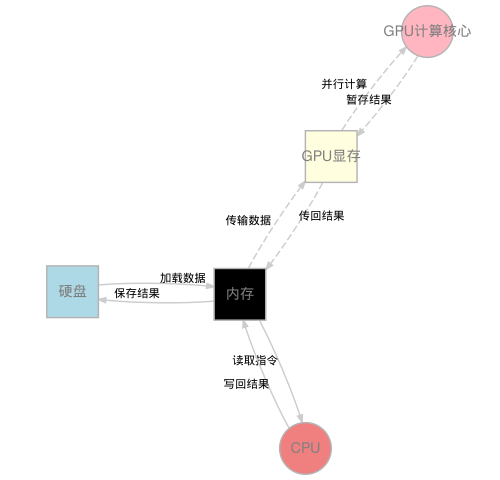
\includegraphics[width=6.94in]{imgs/hardware_flow} \caption{程序运行中的数据流动示意图}\label{fig:hardware-flow-export}
\end{figure}

图\ref{fig:hardware-flow-export} 展示了程序运行过程中数据在不同硬件组件间的流动路径。在统计分析的具体场景中,这种数据流转体现得更加明显。例如,当运行一个线性回归分析时:R解释器从硬盘读取脚本文件到内存;数据文件从硬盘加载到内存的数据框中;CPU执行lm()函数,在内存中进行矩阵运算;计算结果(系数、p值等)存储在内存中的模型对象里;最终结果被写入硬盘的报告文件。如果分析涉及大规模数据,可能会出现内存瓶颈,此时需要采用分批处理或流式处理策略,让数据在硬盘和内存间分块流动。

理解硬件组成和程序运行流程有助于统计分析人员优化工作流程。例如,知道CPU多核特性可以指导使用并行计算包(如parallel)来加速计算;了解GPU的并行能力可以指导选择适合GPU加速的算法;认识内存限制可以避免处理过大的数据集导致系统崩溃;理解硬盘性能差异可以优化数据存储策略。这种硬件意识是现代数据科学家必备的基础知识,它帮助研究者在技术约束下做出明智的决策,确保统计分析既高效又可靠。

\hypertarget{ux53d8ux91cfux4e0eux5e38ux91cf}{%
\subsubsection{变量与常量}\label{ux53d8ux91cfux4e0eux5e38ux91cf}}

\begin{Shaded}
\begin{Highlighting}[]
\CommentTok{\# 变量就像可擦写的白板,可以随时修改}
\NormalTok{score }\OtherTok{\textless{}{-}} \DecValTok{90}
\NormalTok{score }\OtherTok{\textless{}{-}} \DecValTok{95} \CommentTok{\# 可以修改}

\CommentTok{\# 常量就像刻在石头上的字,一旦设定就不能改变}
\NormalTok{PI }\OtherTok{\textless{}{-}} \FloatTok{3.14159}
\CommentTok{\# PI \textless{}{-} 3.14  \# 不应该修改常量}
\end{Highlighting}
\end{Shaded}

变量和常量的区分体现了编程中的抽象思维和工程规范,是构建可维护、可复用代码的基础。在生态学数据分析中,这种区分尤为重要。变量就像生态学研究中的测量指标------它们会随着时间、空间或处理条件而变化,比如样地的温度读数、物种的个体数量、实验处理的效果值等。使用变量可以让代码适应不同的数据输入,实现分析的通用性和灵活性。而常量则代表那些在特定分析中保持不变的基础参数,比如圆周率π、重力加速度g、或者生态学中常用的转换系数(如生物量估算公式中的参数)。这些常量一旦设定就不应该被修改,因为它们代表了科学共识或物理规律。

从工程角度看,正确使用常量可以避免''魔法数字''问题------在代码中直接使用未经解释的数值,这不仅降低了代码的可读性,还增加了出错风险。比如,在计算森林碳储量时,如果直接将碳转换系数0.5写在计算公式中,其他研究者很难理解这个数字的含义,而且如果后续研究更新了这个系数,就需要在整个代码中搜索并修改所有出现0.5的地方。而如果将其定义为常量\texttt{CARBON\_CONVERSION\_FACTOR\ \textless{}-\ 0.5},代码就变得自文档化,修改也只需要在一个地方进行。

在生态学编程实践中,变量和常量的恰当使用还体现了对数据生命周期的理解。变量通常对应着分析过程中的中间结果或输入数据,它们的值会在分析流程中不断变化;而常量则对应着分析的基本假设和约束条件,它们定义了分析的边界和前提。这种区分有助于建立清晰的思维框架,让研究者能够更好地组织分析逻辑,确保代码的科学性和可复现性。更重要的是,在现代AI辅助编程环境中,明确的变量常量区分能够帮助LLM更好地理解代码意图,生成更符合生态学研究规范的解决方案。

\hypertarget{ux57faux672cux6570ux636eux7c7bux578b}{%
\subsubsection{基本数据类型}\label{ux57faux672cux6570ux636eux7c7bux578b}}

\begin{Shaded}
\begin{Highlighting}[]
\CommentTok{\# 数字类型}
\NormalTok{temperature }\OtherTok{\textless{}{-}} \FloatTok{25.5}
\NormalTok{count }\OtherTok{\textless{}{-}} \DecValTok{100}\DataTypeTok{L}

\CommentTok{\# 逻辑类型}
\NormalTok{is\_raining }\OtherTok{\textless{}{-}} \ConstantTok{TRUE}
\NormalTok{is\_sunny }\OtherTok{\textless{}{-}} \ConstantTok{FALSE}

\CommentTok{\# 字符类型}
\NormalTok{species\_name }\OtherTok{\textless{}{-}} \StringTok{"Quercus acutissima"}
\NormalTok{habitat }\OtherTok{\textless{}{-}} \StringTok{"deciduous forest"}

\CommentTok{\# 空值}
\NormalTok{missing\_data }\OtherTok{\textless{}{-}} \ConstantTok{NULL}
\end{Highlighting}
\end{Shaded}

数据类型的正确理解和使用是生态学数据分析的基石,它直接影响分析的准确性、效率和可解释性。在生态学研究中,不同类型的数据对应着不同的统计方法和生态学意义,混淆数据类型可能导致严重的科学错误。比如,物种名称是分类数据(字符型),应该使用频数统计和卡方检验;个体数量是计数数据(整数型),适合使用泊松回归或负二项回归;环境温度是连续数据(数值型),可以使用相关分析和回归模型;而存在/缺失数据(逻辑型)则需要使用二元响应模型。

从技术层面看,数据类型决定了可用的操作和函数。对数值型数据可以进行算术运算、统计检验和数学变换;对字符型数据可以进行字符串处理、模式匹配和分类汇总;对逻辑型数据可以进行逻辑运算和条件筛选。如果混淆了数据类型,比如试图对物种名称进行算术平均,或者对温度数据进行字符串拼接,不仅会产生无意义的结果,还可能导致程序错误。更重要的是,在生态学数据分析中,数据类型的选择往往反映了对生态现象的深刻理解------比如将连续的环境梯度离散化为分类变量时,需要基于生态学理论来确定分类边界。

在AI辅助编程时代,数据类型知识变得更加重要。当向LLM描述分析需求时,明确的数据类型说明能够帮助AI生成更准确的代码。比如,``分析温度对物种丰富度的影响''这个需求中,如果明确指出温度是连续变量,物种丰富度是计数变量,LLM就会推荐使用广义线性模型而不是普通的线性回归。此外,数据类型还关系到数据存储效率和计算性能------数值型数据比字符型数据占用更少内存,整数运算比浮点运算更快。在处理大规模的生态监测数据时,这种效率差异可能决定分析是否可行。因此,掌握数据类型不仅是编程技术问题,更是生态学研究者科学素养的体现。

\hypertarget{ux8fd0ux7b97ux7b26}{%
\subsubsection{运算符}\label{ux8fd0ux7b97ux7b26}}

\begin{Shaded}
\begin{Highlighting}[]
\CommentTok{\# 先定义示例数据}
\NormalTok{dbh }\OtherTok{\textless{}{-}} \FloatTok{25.3} \CommentTok{\# 胸径}
\NormalTok{height }\OtherTok{\textless{}{-}} \FloatTok{18.2} \CommentTok{\# 树高}
\NormalTok{species1 }\OtherTok{\textless{}{-}} \StringTok{"Quercus"}
\NormalTok{species2 }\OtherTok{\textless{}{-}} \StringTok{"Pinus"}
\NormalTok{temperature }\OtherTok{\textless{}{-}} \DecValTok{20}
\NormalTok{rainfall }\OtherTok{\textless{}{-}} \DecValTok{1200}
\NormalTok{abundance }\OtherTok{\textless{}{-}} \DecValTok{5}
\NormalTok{distribution\_area }\OtherTok{\textless{}{-}} \DecValTok{80}
\NormalTok{species\_list }\OtherTok{\textless{}{-}} \FunctionTok{c}\NormalTok{(}\StringTok{"Quercus"}\NormalTok{, }\StringTok{"Pinus"}\NormalTok{, }\StringTok{"Acer"}\NormalTok{, }\StringTok{"Betula"}\NormalTok{, }\StringTok{"Fagus"}\NormalTok{)}

\CommentTok{\# 算术运算符}
\NormalTok{biomass }\OtherTok{\textless{}{-}}\NormalTok{ dbh}\SpecialCharTok{\^{}}\DecValTok{2} \SpecialCharTok{*}\NormalTok{ height }\SpecialCharTok{*} \FloatTok{0.6} \CommentTok{\# 幂运算和乘法}

\CommentTok{\# 比较运算符}
\NormalTok{is\_large\_tree }\OtherTok{\textless{}{-}}\NormalTok{ dbh }\SpecialCharTok{\textgreater{}} \DecValTok{30} \CommentTok{\# 大于比较}
\NormalTok{is\_same\_species }\OtherTok{\textless{}{-}}\NormalTok{ species1 }\SpecialCharTok{==}\NormalTok{ species2 }\CommentTok{\# 相等比较}

\CommentTok{\# 逻辑运算符}
\NormalTok{suitable\_habitat }\OtherTok{\textless{}{-}}\NormalTok{ (temperature }\SpecialCharTok{\textgreater{}} \DecValTok{15}\NormalTok{) }\SpecialCharTok{\&}\NormalTok{ (rainfall }\SpecialCharTok{\textgreater{}} \DecValTok{1000}\NormalTok{) }\CommentTok{\# 与运算}
\NormalTok{rare\_species }\OtherTok{\textless{}{-}}\NormalTok{ (abundance }\SpecialCharTok{\textless{}} \DecValTok{10}\NormalTok{) }\SpecialCharTok{|}\NormalTok{ (distribution\_area }\SpecialCharTok{\textless{}} \DecValTok{100}\NormalTok{) }\CommentTok{\# 或运算}

\CommentTok{\# 赋值运算符}
\NormalTok{species\_count }\OtherTok{\textless{}{-}} \FunctionTok{length}\NormalTok{(}\FunctionTok{unique}\NormalTok{(species\_list)) }\CommentTok{\# 常规赋值}
\end{Highlighting}
\end{Shaded}

运算符是编程语言中执行基本操作的核心元素,它们将简单的数据值组合成复杂的计算表达式。在生态学数据分析中,运算符的正确使用直接关系到分析结果的准确性和科学性。运算符可以分为几个主要类别:算术运算符(+、-、*、/、\^{})用于数值计算,如生物量估算、种群密度计算;比较运算符(\textgreater、\textless、==、!=)用于条件判断,如筛选特定大小的树木或特定温度范围的数据;逻辑运算符(\&、\textbar、!)用于组合多个条件,如同时满足温度和湿度要求的生态位分析。

运算符的优先级和结合性规则决定了复杂表达式的计算顺序,理解这些规则对于编写正确的代码至关重要。比如在表达式\texttt{a\ +\ b\ *\ c}中,乘法优先级高于加法,会先计算\texttt{b\ *\ c}再与\texttt{a}相加。如果不理解优先级,可能导致计算结果错误。在生态学建模中,这种精确性尤为重要------错误的运算符使用可能导致模型偏差或生态学意义的误解。

在AI协作环境中,明确的运算符使用能够显著提高与LLM的沟通效率。当向AI描述分析需求时,使用正确的运算符术语(如''使用逻辑与运算符组合温度和降水条件'')比模糊的描述(如''同时考虑温度和降水'')能生成更准确的代码。运算符还是连接数据与算法的桥梁,它们将原始生态数据转化为有意义的生态指标,是构建科学分析流程的基础构件。掌握运算符的使用不仅是一项编程技能,更是生态学研究者表达分析逻辑的重要工具。

\hypertarget{ux96c6ux5408ux6570ux636eux7c7bux578b}{%
\subsubsection{集合数据类型}\label{ux96c6ux5408ux6570ux636eux7c7bux578b}}

\begin{Shaded}
\begin{Highlighting}[]
\CommentTok{\# 向量 {-} 同类型元素的集合}
\NormalTok{temperatures }\OtherTok{\textless{}{-}} \FunctionTok{c}\NormalTok{(}\DecValTok{20}\NormalTok{, }\DecValTok{22}\NormalTok{, }\DecValTok{25}\NormalTok{, }\DecValTok{18}\NormalTok{, }\DecValTok{23}\NormalTok{)}
\NormalTok{species }\OtherTok{\textless{}{-}} \FunctionTok{c}\NormalTok{(}\StringTok{"Oak"}\NormalTok{, }\StringTok{"Pine"}\NormalTok{, }\StringTok{"Maple"}\NormalTok{, }\StringTok{"Birch"}\NormalTok{)}

\CommentTok{\# 列表 {-} 可以包含不同类型的元素}
\NormalTok{forest\_data }\OtherTok{\textless{}{-}} \FunctionTok{list}\NormalTok{(}
  \AttributeTok{name =} \StringTok{"Tianmu Mountain Forest"}\NormalTok{,}
  \AttributeTok{area =} \DecValTok{428}\NormalTok{,}
  \AttributeTok{dominant\_species =} \FunctionTok{c}\NormalTok{(}\StringTok{"Cyclobalanopsis"}\NormalTok{, }\StringTok{"Castanopsis"}\NormalTok{),}
  \AttributeTok{elevation\_range =} \FunctionTok{c}\NormalTok{(}\DecValTok{300}\NormalTok{, }\DecValTok{1500}\NormalTok{)}
\NormalTok{)}

\CommentTok{\# 数据框 {-} 表格形式的数据}
\NormalTok{forest\_df }\OtherTok{\textless{}{-}} \FunctionTok{data.frame}\NormalTok{(}
  \AttributeTok{plot\_id =} \DecValTok{1}\SpecialCharTok{:}\DecValTok{5}\NormalTok{,}
  \AttributeTok{species =} \FunctionTok{c}\NormalTok{(}\StringTok{"Quercus"}\NormalTok{, }\StringTok{"Pinus"}\NormalTok{, }\StringTok{"Acer"}\NormalTok{, }\StringTok{"Betula"}\NormalTok{, }\StringTok{"Fagus"}\NormalTok{),}
  \AttributeTok{dbh =} \FunctionTok{c}\NormalTok{(}\FloatTok{25.3}\NormalTok{, }\FloatTok{18.7}\NormalTok{, }\FloatTok{12.4}\NormalTok{, }\FloatTok{15.8}\NormalTok{, }\FloatTok{22.1}\NormalTok{),}
  \AttributeTok{height =} \FunctionTok{c}\NormalTok{(}\FloatTok{18.2}\NormalTok{, }\FloatTok{15.6}\NormalTok{, }\FloatTok{10.3}\NormalTok{, }\FloatTok{12.7}\NormalTok{, }\FloatTok{16.9}\NormalTok{)}
\NormalTok{)}
\end{Highlighting}
\end{Shaded}

集合数据类型的正确选择是生态学数据分析效率和质量的关键,它体现了对数据结构复杂性和分析需求的深刻理解。与基本数据类型(如数值、字符、逻辑值)处理单个数据元素不同,集合数据类型用于组织和存储多个相关数据,每种类型都有其独特的结构特性和适用场景。在生态学研究中,这种区分尤为重要------向量适合存储同类型的观测序列(如连续的温度读数),列表能够容纳复杂的嵌套结构(如包含样地信息、物种组成、环境因子的综合数据),而数据框则专门为表格型数据设计(如样地调查表)。

基本数据类型与集合数据类型的根本区别在于组织层次和操作粒度。基本数据类型关注单个数据点的属性和操作,比如数值的算术运算、字符的字符串处理;而集合数据类型关注数据之间的组织关系和整体操作,比如向量的元素索引、列表的嵌套访问、数据框的行列筛选。这种区别决定了它们的使用场景:当需要处理单一类型的序列数据时,向量提供了高效的内存存储和向量化运算;当数据结构复杂且异构时,列表的灵活性允许存储不同类型的数据对象;当数据呈现表格形式且需要同时处理多个变量时,数据框的结构化存储便于统计分析。

在生态学数据分析实践中,正确的集合类型选择直接影响分析效率和结果质量。比如,使用向量存储物种多样性指数序列可以实现快速的统计计算和可视化;使用列表组织不同样地的监测数据便于批量处理和比较分析;使用数据框管理样地调查表则可以直接应用各种统计函数和机器学习算法。更重要的是,集合数据类型的选择反映了对生态数据本质的理解------是时间序列、空间分布还是多变量关系?这种理解有助于设计更合理的分析流程,确保统计方法的适用性和结果的科学性。在AI协作环境中,明确的集合类型说明能够帮助LLM生成更符合生态学数据分析规范的代码,提高协作效率。

\hypertarget{ux5206ux652fux4e0eux5faaux73af}{%
\subsubsection{分支与循环}\label{ux5206ux652fux4e0eux5faaux73af}}

\begin{Shaded}
\begin{Highlighting}[]
\CommentTok{\# 条件判断 {-} 根据条件选择不同路径}
\NormalTok{classify\_tree\_size }\OtherTok{\textless{}{-}} \ControlFlowTok{function}\NormalTok{(dbh) \{}
  \ControlFlowTok{if}\NormalTok{ (dbh }\SpecialCharTok{\textless{}} \DecValTok{10}\NormalTok{) \{}
    \FunctionTok{return}\NormalTok{(}\StringTok{"sapling"}\NormalTok{)}
\NormalTok{  \} }\ControlFlowTok{else} \ControlFlowTok{if}\NormalTok{ (dbh }\SpecialCharTok{\textless{}} \DecValTok{30}\NormalTok{) \{}
    \FunctionTok{return}\NormalTok{(}\StringTok{"medium tree"}\NormalTok{)}
\NormalTok{  \} }\ControlFlowTok{else}\NormalTok{ \{}
    \FunctionTok{return}\NormalTok{(}\StringTok{"large tree"}\NormalTok{)}
\NormalTok{  \}}
\NormalTok{\}}

\CommentTok{\# 循环 {-} 重复执行操作}
\CommentTok{\# 计算每个样地的平均胸径}
\NormalTok{plot\_dbh }\OtherTok{\textless{}{-}} \FunctionTok{c}\NormalTok{(}\FloatTok{15.3}\NormalTok{, }\FloatTok{22.7}\NormalTok{, }\FloatTok{18.4}\NormalTok{, }\FloatTok{25.1}\NormalTok{, }\FloatTok{12.9}\NormalTok{)}
\NormalTok{average\_dbh }\OtherTok{\textless{}{-}} \FunctionTok{numeric}\NormalTok{(}\FunctionTok{length}\NormalTok{(plot\_dbh))}

\ControlFlowTok{for}\NormalTok{ (i }\ControlFlowTok{in} \FunctionTok{seq\_along}\NormalTok{(plot\_dbh)) \{}
\NormalTok{  average\_dbh[i] }\OtherTok{\textless{}{-}} \FunctionTok{mean}\NormalTok{(plot\_dbh[}\DecValTok{1}\SpecialCharTok{:}\NormalTok{i])}
\NormalTok{\}}

\CommentTok{\# 更R风格的方式 {-} 使用向量化操作}
\NormalTok{average\_dbh }\OtherTok{\textless{}{-}} \FunctionTok{cumsum}\NormalTok{(plot\_dbh) }\SpecialCharTok{/} \FunctionTok{seq\_along}\NormalTok{(plot\_dbh)}
\end{Highlighting}
\end{Shaded}

分支与循环是构建复杂生态学数据分析逻辑的核心工具,它们将静态的数据处理转化为动态的、智能的分析流程。在生态学研究中,自然系统的复杂性和不确定性要求分析程序能够根据数据特征自动调整处理策略,这正是分支结构的价值所在。比如,在分析物种分布数据时,可能需要根据数据质量(完整性、准确性)选择不同的预处理方法;在处理环境梯度数据时,需要根据变量类型(连续型、分类型)应用不同的统计模型。这种条件判断能力使得分析程序能够适应真实世界的复杂性,而不是僵化地套用固定流程。

循环结构则解决了生态学数据分析中的规模化问题。生态学研究往往涉及大量的重复性操作------对数百个样地的数据执行相同的计算,对数十个环境变量进行相同的统计分析,对多年的监测数据进行相同的时间序列分析。手动重复这些操作不仅效率低下,还容易出错。循环结构通过自动化这些重复任务,确保了分析的一致性和可复现性。更重要的是,在R语言中,向量化操作往往比显式循环更高效,这体现了对计算效率的深入理解。

分支与循环的组合使用能够构建出真正智能的数据分析系统。比如,一个完整的生态数据分析流程可能包含:首先使用循环遍历所有样地,对每个样地使用分支结构检查数据质量,然后根据质量等级选择不同的清洗策略,接着使用嵌套循环分析不同时间尺度的变化模式,最后根据统计显著性自动生成报告结论。这种复杂的逻辑结构正是现代生态学研究所需的------它能够处理大规模、多维度、异质性的生态数据,产生科学可靠的结论。在AI协作时代,理解这些控制结构有助于更好地指导LLM生成符合生态学分析逻辑的代码,而不是简单的脚本堆积。

\textbf{向量化操作的重要性}:在R语言中,向量化操作代表了更高级的编程思维,它通过将操作应用于整个数据向量而非单个元素,极大地简化了数据分析代码。对于生态学研究者而言,向量化不仅意味着代码简洁性的提升------比如用\texttt{mean(temperature)}替代繁琐的循环计算,更重要的是它体现了对数据整体性的理解。在处理生态监测数据时,向量化操作允许研究者一次性对整个时间序列或空间网格进行分析,而不是逐点处理,这大大提高了代码的可读性和可维护性。

从性能角度看,向量化操作通常比显式循环运行更快,因为R的内部优化能够利用底层C/Fortran代码的高效实现。这种性能优势在R、Python等解释型语言中尤为明显,因为这些语言中的循环通常较慢。相比之下,在C++等编译型语言中,循环本身已经高度优化,向量化的性能优势相对较小,但向量化思维仍然有助于简化代码语法。在处理大规模的生态数据集(如遥感影像、长期监测记录)时,这种速度优势可能决定分析是否可行。然而,向量化操作也有其局限性:它要求数据具有相同的结构和类型,对于复杂的分支逻辑或条件处理可能不够灵活。此外,过度向量化可能降低代码的可调试性,因为错误可能隐藏在复杂的向量运算中。另一个重要缺陷是内存消耗问题:向量化操作通常需要将整个数据集加载到内存中进行批量处理,对于超大规模的生态数据集(如高分辨率遥感影像、全基因组序列),这可能超出计算机的内存容量,导致程序崩溃。相比之下,循环处理可以逐块读取数据,减少内存压力。因此,生态学研究者需要在向量化的简洁高效与循环的灵活可控之间找到平衡,根据具体分析需求选择最合适的编程范式。

\hypertarget{ux8868ux8fbeux5f0fux4e0eux8bedux53e5}{%
\subsubsection{表达式与语句}\label{ux8868ux8fbeux5f0fux4e0eux8bedux53e5}}

\begin{Shaded}
\begin{Highlighting}[]
\CommentTok{\# 表达式 {-} 产生值的代码片段}
\NormalTok{total\_trees }\OtherTok{\textless{}{-}} \DecValTok{100} \SpecialCharTok{+} \DecValTok{50} \CommentTok{\# 表达式,产生值150}
\NormalTok{mean\_dbh }\OtherTok{\textless{}{-}} \FunctionTok{mean}\NormalTok{(}\FunctionTok{c}\NormalTok{(}\DecValTok{25}\NormalTok{, }\DecValTok{30}\NormalTok{, }\DecValTok{35}\NormalTok{)) }\CommentTok{\# 表达式,产生平均值}

\CommentTok{\# 语句 {-} 执行动作的代码单元}
\ControlFlowTok{if}\NormalTok{ (temperature }\SpecialCharTok{\textgreater{}} \DecValTok{25}\NormalTok{) \{}
  \FunctionTok{cat}\NormalTok{(}\StringTok{"温度过高,需要调整实验条件}\SpecialCharTok{\textbackslash{}n}\StringTok{"}\NormalTok{) }\CommentTok{\# 语句}
\NormalTok{\}}

\CommentTok{\# 定义示例数据和函数}
\NormalTok{plots }\OtherTok{\textless{}{-}} \FunctionTok{c}\NormalTok{(}\StringTok{"plot1"}\NormalTok{, }\StringTok{"plot2"}\NormalTok{, }\StringTok{"plot3"}\NormalTok{)}
\NormalTok{analyze\_plot }\OtherTok{\textless{}{-}} \ControlFlowTok{function}\NormalTok{(plot) \{}
  \FunctionTok{cat}\NormalTok{(}\StringTok{"分析样地:"}\NormalTok{, plot, }\StringTok{"}\SpecialCharTok{\textbackslash{}n}\StringTok{"}\NormalTok{)}
\NormalTok{\}}

\ControlFlowTok{for}\NormalTok{ (plot }\ControlFlowTok{in}\NormalTok{ plots) \{}
  \FunctionTok{analyze\_plot}\NormalTok{(plot) }\CommentTok{\# 语句}
\NormalTok{\}}
\end{Highlighting}
\end{Shaded}

\begin{verbatim}
## 分析样地: plot1 
## 分析样地: plot2 
## 分析样地: plot3
\end{verbatim}

表达式与语句的区分体现了编程中的两种基本思维模式------计算思维和流程控制思维。表达式(Expression)是能够产生值的代码片段,它们关注''计算什么'',通过运算符和函数调用来完成具体的数值计算或逻辑判断。比如\texttt{dbh\^{}2\ *\ height\ *\ 0.6}是一个表达式,它计算树木的生物量;\texttt{temperature\ \textgreater{}\ 25}也是一个表达式,它产生逻辑值TRUE或FALSE。表达式可以嵌套组合,形成复杂的计算逻辑,但最终都会归结为一个具体的值。

语句(Statement)则是执行动作的代码单元,它们关注''做什么'',控制程序的执行流程。语句不产生值(或者产生的值不是其主要目的),而是完成特定的操作任务。前面提到的分支(if-else)和循环(for/while)都是典型的语句类型------分支语句根据条件选择不同的执行路径,循环语句重复执行特定的代码块。其他常见的语句还包括赋值语句(\texttt{x\ \textless{}-\ 10})、函数调用语句等。

这种区分在生态学数据分析中尤为重要:表达式用于构建统计模型和计算生态指标,如多样性指数计算、回归分析等;语句则用于控制分析流程,如根据数据质量选择不同的预处理方法,或者对多个样地执行相同的分析操作。理解这种区别有助于设计更清晰的分析架构,也便于与LLM有效协作------明确告诉AI需要计算什么(表达式)和需要执行什么操作(语句)。

\hypertarget{ux51fdux6570ux8fc7ux7a0b}{%
\subsubsection{函数/过程}\label{ux51fdux6570ux8fc7ux7a0b}}

\begin{Shaded}
\begin{Highlighting}[]
\CommentTok{\# 加载必要的包}
\FunctionTok{library}\NormalTok{(dplyr)}
\end{Highlighting}
\end{Shaded}

\begin{verbatim}
## 
## Attaching package: 'dplyr'
\end{verbatim}

\begin{verbatim}
## The following objects are masked from 'package:stats':
## 
##     filter, lag
\end{verbatim}

\begin{verbatim}
## The following objects are masked from 'package:base':
## 
##     intersect, setdiff, setequal, union
\end{verbatim}

\begin{Shaded}
\begin{Highlighting}[]
\FunctionTok{library}\NormalTok{(stringr)}

\CommentTok{\# 定义计算物种多样性的函数}
\NormalTok{calculate\_diversity }\OtherTok{\textless{}{-}} \ControlFlowTok{function}\NormalTok{(species\_list) \{}
\NormalTok{  species\_counts }\OtherTok{\textless{}{-}} \FunctionTok{table}\NormalTok{(species\_list)}
\NormalTok{  proportions }\OtherTok{\textless{}{-}}\NormalTok{ species\_counts }\SpecialCharTok{/} \FunctionTok{sum}\NormalTok{(species\_counts)}
\NormalTok{  shannon }\OtherTok{\textless{}{-}} \SpecialCharTok{{-}}\FunctionTok{sum}\NormalTok{(proportions }\SpecialCharTok{*} \FunctionTok{log}\NormalTok{(proportions))}
  \FunctionTok{return}\NormalTok{(shannon)}
\NormalTok{\}}

\CommentTok{\# 定义数据清洗函数}
\NormalTok{clean\_forest\_data }\OtherTok{\textless{}{-}} \ControlFlowTok{function}\NormalTok{(raw\_data) \{}
\NormalTok{  cleaned }\OtherTok{\textless{}{-}}\NormalTok{ raw\_data }\SpecialCharTok{\%\textgreater{}\%}
    \FunctionTok{filter}\NormalTok{(}\SpecialCharTok{!}\FunctionTok{is.na}\NormalTok{(dbh) }\SpecialCharTok{\&}\NormalTok{ dbh }\SpecialCharTok{\textgreater{}} \DecValTok{0}\NormalTok{) }\SpecialCharTok{\%\textgreater{}\%}
    \FunctionTok{mutate}\NormalTok{(}\AttributeTok{species =} \FunctionTok{str\_trim}\NormalTok{(}\FunctionTok{tolower}\NormalTok{(species)))}
  \FunctionTok{return}\NormalTok{(cleaned)}
\NormalTok{\}}

\CommentTok{\# 创建示例数据}
\NormalTok{raw\_forest\_data }\OtherTok{\textless{}{-}} \FunctionTok{data.frame}\NormalTok{(}
  \AttributeTok{plot\_id =} \DecValTok{1}\SpecialCharTok{:}\DecValTok{5}\NormalTok{,}
  \AttributeTok{species =} \FunctionTok{c}\NormalTok{(}\StringTok{" Oak "}\NormalTok{, }\StringTok{"Pine "}\NormalTok{, }\StringTok{" Maple"}\NormalTok{, }\StringTok{"Oak"}\NormalTok{, }\StringTok{" Birch "}\NormalTok{),}
  \AttributeTok{dbh =} \FunctionTok{c}\NormalTok{(}\FloatTok{25.3}\NormalTok{, }\FloatTok{18.7}\NormalTok{, }\ConstantTok{NA}\NormalTok{, }\FloatTok{15.8}\NormalTok{, }\FloatTok{22.1}\NormalTok{),}
  \AttributeTok{height =} \FunctionTok{c}\NormalTok{(}\FloatTok{18.2}\NormalTok{, }\FloatTok{15.6}\NormalTok{, }\FloatTok{10.3}\NormalTok{, }\FloatTok{12.7}\NormalTok{, }\FloatTok{16.9}\NormalTok{)}
\NormalTok{)}

\CommentTok{\# 使用函数}
\NormalTok{sample\_species }\OtherTok{\textless{}{-}} \FunctionTok{c}\NormalTok{(}\StringTok{"Oak"}\NormalTok{, }\StringTok{"Pine"}\NormalTok{, }\StringTok{"Oak"}\NormalTok{, }\StringTok{"Maple"}\NormalTok{)}
\NormalTok{diversity\_index }\OtherTok{\textless{}{-}} \FunctionTok{calculate\_diversity}\NormalTok{(sample\_species)}
\NormalTok{cleaned\_data }\OtherTok{\textless{}{-}} \FunctionTok{clean\_forest\_data}\NormalTok{(raw\_forest\_data)}
\end{Highlighting}
\end{Shaded}

函数是编程中的抽象工具,它将复杂的操作封装成可重用的模块,体现了''一次编写,多次使用''的工程原则。在生态学数据分析中,函数的使用具有多重价值:首先是代码复用性------相同的分析逻辑可以在不同项目、不同数据集中重复使用,避免重复劳动。比如,一个计算Shannon多样性指数的函数可以在多个森林调查项目中重复使用,大大提高了分析效率。其次是可维护性------当分析逻辑需要修改时,只需修改函数定义,所有调用该函数的地方都会自动更新。例如,如果需要改进多样性指数的计算方法,只需修改\texttt{calculate\_diversity}函数,而不需要在每个使用该计算的地方逐一修改。再次是模块化设计------通过将复杂分析流程分解为多个函数,使代码结构更清晰,便于理解和调试。在生态学研究中,一个完整的分析流程可能包含数据读取、清洗、多样性计算、统计检验、可视化等多个步骤,每个步骤都可以封装为独立的函数,使整体分析逻辑更加清晰。

从工程角度看,函数还促进了代码的标准化和规范化。在团队协作的生态学研究项目中,统一的函数接口可以确保不同研究者使用相同的分析方法,提高结果的可比性和可复现性。例如,定义标准的\texttt{clean\_forest\_data}函数可以确保所有参与者在数据清洗阶段采用相同的质量控制标准。

在AI协作环境中,函数思维变得更加重要。当向LLM描述分析需求时,明确的函数化架构能够帮助AI更好地理解分析逻辑,生成更模块化、可维护的代码。LLM可以根据函数化的需求描述,分别生成数据读取、处理、分析、可视化等各个模块的代码,而不是生成一个冗长复杂的单一脚本。这种模块化的代码结构不仅便于人类理解,也便于后续的调试和优化。更重要的是,函数化的思维有助于建立清晰的测试框架------每个函数都可以独立测试,确保其功能的正确性,从而提高整个分析流程的可靠性。在生态学数据分析的复杂环境中,这种函数化的设计思维是确保分析质量、提高协作效率的关键保障。

\hypertarget{ux4f5cux7528ux57df}{%
\subsubsection{作用域}\label{ux4f5cux7528ux57df}}

\begin{Shaded}
\begin{Highlighting}[]
\CommentTok{\# 全局变量}
\NormalTok{global\_species\_count }\OtherTok{\textless{}{-}} \DecValTok{0}

\NormalTok{analyze\_forest }\OtherTok{\textless{}{-}} \ControlFlowTok{function}\NormalTok{(plot\_data) \{}
  \CommentTok{\# 局部变量 {-} 只在函数内部可见}
\NormalTok{  local\_species }\OtherTok{\textless{}{-}} \FunctionTok{unique}\NormalTok{(plot\_data}\SpecialCharTok{$}\NormalTok{species)}
\NormalTok{  local\_count }\OtherTok{\textless{}{-}} \FunctionTok{length}\NormalTok{(local\_species)}

  \CommentTok{\# 可以访问全局变量}
\NormalTok{  global\_species\_count }\OtherTok{\textless{}\textless{}{-}}\NormalTok{ global\_species\_count }\SpecialCharTok{+}\NormalTok{ local\_count}

  \FunctionTok{return}\NormalTok{(local\_count)}
\NormalTok{\}}

\CommentTok{\# 在函数外部无法访问局部变量}
\CommentTok{\# print(local\_species)  \# 会报错}

\CommentTok{\# 但可以访问全局变量}
\FunctionTok{print}\NormalTok{(global\_species\_count)}
\end{Highlighting}
\end{Shaded}

\begin{verbatim}
## [1] 0
\end{verbatim}

作用域规则定义了变量的可见范围,是构建复杂、安全程序的基础机制。在生态学数据分析中,正确理解作用域具有多重重要意义:首先,作用域机制有效避免了命名冲突------不同的函数或模块可以使用相同的变量名而不会相互干扰。例如,在分析多个样地数据时,每个样地的分析函数都可以使用\texttt{species\_count}作为局部变量,而不会影响其他样地的计算结果。这种隔离性大大简化了变量命名,降低了代码复杂度。

其次,作用域提供了精细的数据访问控制能力。在生态学研究中,某些敏感数据(如原始调查记录、物种分布坐标等)需要限制访问范围,防止意外修改或泄露。通过将敏感数据封装在特定作用域内,可以确保只有授权的函数能够访问和修改这些数据,提高了代码的安全性。

第三,作用域规则优化了内存管理效率。局部变量在函数执行结束时自动释放,避免了内存泄漏问题。在处理大规模的生态监测数据时,这种自动内存管理机制尤为重要,可以防止因变量积累导致的内存耗尽问题。例如,在循环处理多个年份的监测数据时,每次迭代的临时变量都会在迭代结束后自动清理,确保内存使用的高效性。

从软件工程角度看,作用域概念体现了信息隐藏原则,是构建模块化、健壮分析系统的关键。通过将内部实现细节隐藏在局部作用域中,只暴露必要的接口,可以降低模块间的耦合度,提高代码的可维护性和可扩展性。在团队协作的生态学研究项目中,明确的作用域规则可以防止意外的变量修改,确保不同开发者编写的代码能够安全地集成在一起。特别是在AI协作环境中,清晰的作用域设计有助于LLM生成更结构化的代码,避免全局变量污染和意外的副作用,从而提高生成代码的质量和可靠性。

\hypertarget{ux9519ux8befux4e0eux5f02ux5e38ux5904ux7406}{%
\subsubsection{错误与异常处理}\label{ux9519ux8befux4e0eux5f02ux5e38ux5904ux7406}}

\begin{Shaded}
\begin{Highlighting}[]
\CommentTok{\# 基本的错误处理}
\NormalTok{safe\_division }\OtherTok{\textless{}{-}} \ControlFlowTok{function}\NormalTok{(numerator, denominator) \{}
  \ControlFlowTok{if}\NormalTok{ (denominator }\SpecialCharTok{==} \DecValTok{0}\NormalTok{) \{}
    \FunctionTok{stop}\NormalTok{(}\StringTok{"分母不能为零"}\NormalTok{)}
\NormalTok{  \}}
  \FunctionTok{return}\NormalTok{(numerator }\SpecialCharTok{/}\NormalTok{ denominator)}
\NormalTok{\}}

\CommentTok{\# 使用tryCatch进行异常处理}
\NormalTok{analyze\_with\_safety }\OtherTok{\textless{}{-}} \ControlFlowTok{function}\NormalTok{(data\_file) \{}
\NormalTok{  result }\OtherTok{\textless{}{-}} \FunctionTok{tryCatch}\NormalTok{(}
\NormalTok{    \{}
      \CommentTok{\# 尝试执行可能出错的操作}
\NormalTok{      data }\OtherTok{\textless{}{-}} \FunctionTok{read.csv}\NormalTok{(data\_file)}
\NormalTok{      diversity }\OtherTok{\textless{}{-}} \FunctionTok{calculate\_diversity}\NormalTok{(data}\SpecialCharTok{$}\NormalTok{species)}
      \FunctionTok{return}\NormalTok{(diversity)}
\NormalTok{    \},}
    \AttributeTok{error =} \ControlFlowTok{function}\NormalTok{(e) \{}
      \CommentTok{\# 错误处理}
      \FunctionTok{cat}\NormalTok{(}\StringTok{"分析失败:"}\NormalTok{, e}\SpecialCharTok{$}\NormalTok{message, }\StringTok{"}\SpecialCharTok{\textbackslash{}n}\StringTok{"}\NormalTok{)}
      \FunctionTok{return}\NormalTok{(}\ConstantTok{NA}\NormalTok{)}
\NormalTok{    \},}
    \AttributeTok{warning =} \ControlFlowTok{function}\NormalTok{(w) \{}
      \CommentTok{\# 警告处理}
      \FunctionTok{cat}\NormalTok{(}\StringTok{"警告:"}\NormalTok{, w}\SpecialCharTok{$}\NormalTok{message, }\StringTok{"}\SpecialCharTok{\textbackslash{}n}\StringTok{"}\NormalTok{)}
      \CommentTok{\# 使用示例数据继续执行}
\NormalTok{      sample\_data }\OtherTok{\textless{}{-}} \FunctionTok{c}\NormalTok{(}\StringTok{"Oak"}\NormalTok{, }\StringTok{"Pine"}\NormalTok{, }\StringTok{"Maple"}\NormalTok{)}
      \FunctionTok{return}\NormalTok{(}\FunctionTok{calculate\_diversity}\NormalTok{(sample\_data))}
\NormalTok{    \}}
\NormalTok{  )}

  \FunctionTok{return}\NormalTok{(result)}
\NormalTok{\}}

\CommentTok{\# 使用示例}
\NormalTok{try\_result }\OtherTok{\textless{}{-}} \FunctionTok{analyze\_with\_safety}\NormalTok{(}\StringTok{"missing\_file.csv"}\NormalTok{)}
\end{Highlighting}
\end{Shaded}

\begin{verbatim}
## 警告: cannot open file 'missing_file.csv': No such file or directory
\end{verbatim}

错误与异常处理是构建健壮分析系统的关键机制,它确保程序在遇到意外情况时能够优雅地处理而不是崩溃。在生态学数据分析中,异常处理尤为重要,因为野外数据往往存在各种质量问题------文件缺失、格式错误、数据异常等。生态学研究的数据来源多样,包括野外调查记录、传感器监测、遥感影像等,这些数据在收集、传输和处理过程中容易出现各种问题。例如,野外调查可能因天气原因中断导致数据不完整,传感器可能因故障产生异常值,不同数据源可能使用不同的格式标准。

通过合理的错误处理,可以显著提高程序的稳定性。在复杂的生态数据分析流程中,一个环节的错误不应该导致整个分析流程的崩溃。例如,当处理多个样地的调查数据时,如果某个样地文件损坏或格式错误,异常处理机制可以捕获这个错误,记录问题并继续处理其他样地,而不是让整个批处理作业失败。这种容错能力对于长期生态监测项目尤为重要,因为数据收集往往跨越数年甚至数十年,期间难免会出现各种技术问题。

异常处理还能提供友好的用户体验。相比于直接显示晦涩的技术错误信息,精心设计的异常处理可以给出清晰、有指导意义的提示。例如,当数据文件缺失时,可以提示用户检查文件路径或提供替代数据源;当数据格式错误时,可以指出具体的问题所在并建议修正方法。这种用户友好的错误处理不仅提高了工具的易用性,也降低了非技术用户的使用门槛。

在自动化流程中,异常处理是确保连续运行的关键。生态学研究经常需要处理大规模数据集,如多年的气候监测数据或大范围的遥感影像。在这些场景下,手动干预每个错误是不现实的。通过异常处理机制,程序可以自动跳过问题数据、记录错误日志、尝试替代方案,确保分析流程能够持续运行。例如,在批量计算物种多样性指数时,如果某个样地的数据质量不合格,程序可以自动标记该样地并继续处理其他样地。

在AI生成代码的背景下,添加适当的错误处理是确保代码质量的重要环节。LLM生成的代码往往侧重于功能实现,可能忽略边界情况和异常处理。作为代码审查者,需要特别关注错误处理机制的完整性,确保生成的代码能够应对各种意外情况。同时,在向LLM描述需求时,明确要求包含完善的错误处理逻辑,可以显著提高生成代码的健壮性和实用性。

\hypertarget{ux6a21ux5757ux5316ux4e0eux5305ux7ba1ux7406}{%
\subsubsection{模块化与包管理}\label{ux6a21ux5757ux5316ux4e0eux5305ux7ba1ux7406}}

\begin{Shaded}
\begin{Highlighting}[]
\CommentTok{\# 模块化代码组织}
\CommentTok{\# data\_processing.R {-} 数据处理模块}
\NormalTok{clean\_data }\OtherTok{\textless{}{-}} \ControlFlowTok{function}\NormalTok{(raw\_data) \{}
  \CommentTok{\# 数据清洗逻辑}
  \FunctionTok{return}\NormalTok{(raw\_data)}
\NormalTok{\}}
\NormalTok{normalize\_data }\OtherTok{\textless{}{-}} \ControlFlowTok{function}\NormalTok{(data) \{}
  \CommentTok{\# 数据标准化逻辑}
  \FunctionTok{return}\NormalTok{(data)}
\NormalTok{\}}

\CommentTok{\# analysis.R {-} 分析模块}
\NormalTok{calculate\_diversity }\OtherTok{\textless{}{-}} \ControlFlowTok{function}\NormalTok{(species) \{}
  \CommentTok{\# 多样性计算}
  \ControlFlowTok{if}\NormalTok{ (}\FunctionTok{length}\NormalTok{(species) }\SpecialCharTok{==} \DecValTok{0}\NormalTok{) \{}
    \FunctionTok{return}\NormalTok{(}\DecValTok{0}\NormalTok{)}
\NormalTok{  \}}
\NormalTok{  species\_counts }\OtherTok{\textless{}{-}} \FunctionTok{table}\NormalTok{(species)}
\NormalTok{  proportions }\OtherTok{\textless{}{-}}\NormalTok{ species\_counts }\SpecialCharTok{/} \FunctionTok{sum}\NormalTok{(species\_counts)}
\NormalTok{  shannon }\OtherTok{\textless{}{-}} \SpecialCharTok{{-}}\FunctionTok{sum}\NormalTok{(proportions }\SpecialCharTok{*} \FunctionTok{log}\NormalTok{(proportions))}
  \FunctionTok{return}\NormalTok{(shannon)}
\NormalTok{\}}
\NormalTok{perform\_stat\_test }\OtherTok{\textless{}{-}} \ControlFlowTok{function}\NormalTok{(data) \{}
  \CommentTok{\# 统计检验}
  \FunctionTok{return}\NormalTok{(}\FloatTok{0.05}\NormalTok{)}
\NormalTok{\}}

\CommentTok{\# visualization.R {-} 可视化模块}
\NormalTok{create\_plots }\OtherTok{\textless{}{-}} \ControlFlowTok{function}\NormalTok{(results) \{}
  \CommentTok{\# 图表生成}
  \FunctionTok{return}\NormalTok{(}\ConstantTok{TRUE}\NormalTok{)}
\NormalTok{\}}

\CommentTok{\# 主程序 {-} 协调各个模块}
\CommentTok{\# source("data\_processing.R")  \# 在实际项目中加载模块文件}
\CommentTok{\# source("analysis.R")}
\CommentTok{\# source("visualization.R")}

\CommentTok{\# 使用包管理}
\FunctionTok{library}\NormalTok{(dplyr) }\CommentTok{\# 数据处理}
\FunctionTok{library}\NormalTok{(ggplot2) }\CommentTok{\# 数据可视化}
\FunctionTok{library}\NormalTok{(vegan) }\CommentTok{\# 生态学分析}
\end{Highlighting}
\end{Shaded}

\begin{verbatim}
## Loading required package: permute
\end{verbatim}

模块化与包管理是构建可维护、可扩展分析系统的核心实践。模块化将复杂的分析流程分解为职责单一、接口清晰的代码单元,这种分解思维在生态学数据分析中具有深远的意义。从技术层面看,模块化显著提高了代码的可读性、可测试性和可维护性。一个典型的生态数据分析项目可能包含数据收集、清洗、统计分析、可视化等多个环节,将这些环节模块化后,每个模块都可以独立开发、测试和优化。例如,数据清洗模块可以专注于处理缺失值和异常值,统计分析模块可以专注于算法实现,可视化模块可以专注于图表设计。这种职责分离使得代码结构更加清晰,便于理解和维护。

包管理则代表了现代编程的协作智慧,它充分利用社区资源,避免重复造轮子。在生态学领域,R语言的包生态系统尤为丰富,提供了大量专业工具。vegan包专门用于生态学多样性分析,spatstat包提供了空间点模式分析的完整解决方案,sp包处理空间数据,lme4包实现混合效应模型等。这些经过社区验证的包不仅提供了可靠的功能实现,还包含了最佳实践和标准方法。

特别值得一提的是spatstat包,它本身就是模块化设计的典范。spatstat将复杂的空间统计分析功能分解为多个子包:spatstat.core处理核心的点模式分析功能,spatstat.geom提供几何操作,spatstat.model实现统计模型,spatstat.explore支持探索性分析等。这种精细的模块化设计让用户可以根据具体需求选择性地加载所需功能,避免不必要的内存开销,同时也便于功能的独立开发和维护。

使用这些专业包,研究者可以快速构建复杂的分析流程,而不需要从零开始实现基础功能。例如,计算物种多样性指数时,直接使用vegan包的\texttt{diversity()}函数,既保证了计算准确性,又节省了开发时间。在进行空间点模式分析时,使用spatstat包可以轻松实现Ripley's K函数、对相关函数等复杂的空间统计方法。

在团队协作的生态学研究项目中,模块化架构特别重要。不同研究者可以负责不同模块的开发,如生态学家专注于分析逻辑的实现,程序员专注于技术架构的优化。清晰的模块接口确保了各个部分能够无缝集成,避免了因代码耦合度过高导致的协作困难。同时,模块化支持代码的渐进式改进------可以单独优化某个模块而不影响其他部分,这种灵活性对于长期的研究项目尤为重要。

包管理还促进了分析方法的标准化和可复现性。当整个研究领域都使用相同的分析包时,不同研究的结果具有更好的可比性。例如,如果所有森林生态学研究都使用vegan包计算多样性指数,那么不同研究的结果就可以进行有意义的比较和整合。这种标准化对于生态学知识的积累和科学共识的形成至关重要。

在AI时代,模块化思维变得更加重要。当向LLM描述分析需求时,明确的模块化架构能够帮助AI生成更结构化的代码。LLM可以根据模块化的需求描述,分别生成数据读取、处理、分析、可视化等各个模块的代码,而不是生成一个冗长复杂的单一脚本。这种模块化的代码不仅便于人类理解,也便于后续的调试、优化和扩展。更重要的是,模块化思维有助于建立清晰的测试框架------每个模块都可以独立测试,确保其功能的正确性,从而提高整个分析流程的可靠性。

\hypertarget{ux9762ux5411ux5bf9ux8c61ux57faux7840}{%
\subsubsection{面向对象基础}\label{ux9762ux5411ux5bf9ux8c61ux57faux7840}}

\begin{Shaded}
\begin{Highlighting}[]
\CommentTok{\# 简单的面向对象示例 {-} 使用S3系统}
\CommentTok{\# 定义物种类}
\NormalTok{species }\OtherTok{\textless{}{-}} \ControlFlowTok{function}\NormalTok{(name, abundance, habitat) \{}
  \FunctionTok{structure}\NormalTok{(}\FunctionTok{list}\NormalTok{(}
    \AttributeTok{name =}\NormalTok{ name,}
    \AttributeTok{abundance =}\NormalTok{ abundance,}
    \AttributeTok{habitat =}\NormalTok{ habitat}
\NormalTok{  ), }\AttributeTok{class =} \StringTok{"species"}\NormalTok{)}
\NormalTok{\}}

\CommentTok{\# 定义方法}
\NormalTok{print.species }\OtherTok{\textless{}{-}} \ControlFlowTok{function}\NormalTok{(x) \{}
  \FunctionTok{cat}\NormalTok{(}\StringTok{"物种:"}\NormalTok{, x}\SpecialCharTok{$}\NormalTok{name, }\StringTok{"}\SpecialCharTok{\textbackslash{}n}\StringTok{"}\NormalTok{)}
  \FunctionTok{cat}\NormalTok{(}\StringTok{"多度:"}\NormalTok{, x}\SpecialCharTok{$}\NormalTok{abundance, }\StringTok{"}\SpecialCharTok{\textbackslash{}n}\StringTok{"}\NormalTok{)}
  \FunctionTok{cat}\NormalTok{(}\StringTok{"生境:"}\NormalTok{, x}\SpecialCharTok{$}\NormalTok{habitat, }\StringTok{"}\SpecialCharTok{\textbackslash{}n}\StringTok{"}\NormalTok{)}
\NormalTok{\}}

\CommentTok{\# 使用示例}
\NormalTok{oak }\OtherTok{\textless{}{-}} \FunctionTok{species}\NormalTok{(}\StringTok{"Quercus"}\NormalTok{, }\DecValTok{150}\NormalTok{, }\StringTok{"deciduous\_forest"}\NormalTok{)}
\FunctionTok{print}\NormalTok{(oak)}
\end{Highlighting}
\end{Shaded}

\begin{verbatim}
## 物种: Quercus 
## 多度: 150 
## 生境: deciduous_forest
\end{verbatim}

\begin{Shaded}
\begin{Highlighting}[]
\CommentTok{\# 更现代的R6系统示例}
\FunctionTok{library}\NormalTok{(R6)}

\NormalTok{ForestPlot }\OtherTok{\textless{}{-}} \FunctionTok{R6Class}\NormalTok{(}\StringTok{"ForestPlot"}\NormalTok{,}
  \AttributeTok{public =} \FunctionTok{list}\NormalTok{(}
    \AttributeTok{plot\_id =} \ConstantTok{NULL}\NormalTok{,}
    \AttributeTok{species\_list =} \ConstantTok{NULL}\NormalTok{,}
    \AttributeTok{initialize =} \ControlFlowTok{function}\NormalTok{(plot\_id, species\_list) \{}
\NormalTok{      self}\SpecialCharTok{$}\NormalTok{plot\_id }\OtherTok{\textless{}{-}}\NormalTok{ plot\_id}
\NormalTok{      self}\SpecialCharTok{$}\NormalTok{species\_list }\OtherTok{\textless{}{-}}\NormalTok{ species\_list}
\NormalTok{    \},}
    \AttributeTok{calculate\_diversity =} \ControlFlowTok{function}\NormalTok{() \{}
      \FunctionTok{table}\NormalTok{(self}\SpecialCharTok{$}\NormalTok{species\_list) }\SpecialCharTok{\%\textgreater{}\%} \FunctionTok{diversity}\NormalTok{()}
\NormalTok{    \},}
    \AttributeTok{print\_info =} \ControlFlowTok{function}\NormalTok{() \{}
      \FunctionTok{cat}\NormalTok{(}\StringTok{"样地"}\NormalTok{, self}\SpecialCharTok{$}\NormalTok{plot\_id, }\StringTok{"有"}\NormalTok{, }\FunctionTok{length}\NormalTok{(}\FunctionTok{unique}\NormalTok{(self}\SpecialCharTok{$}\NormalTok{species\_list)), }\StringTok{"个物种}\SpecialCharTok{\textbackslash{}n}\StringTok{"}\NormalTok{)}
\NormalTok{    \}}
\NormalTok{  )}
\NormalTok{)}

\CommentTok{\# 使用示例}
\NormalTok{plot1 }\OtherTok{\textless{}{-}}\NormalTok{ ForestPlot}\SpecialCharTok{$}\FunctionTok{new}\NormalTok{(}\DecValTok{1}\NormalTok{, }\FunctionTok{c}\NormalTok{(}\StringTok{"Oak"}\NormalTok{, }\StringTok{"Pine"}\NormalTok{, }\StringTok{"Oak"}\NormalTok{))}
\NormalTok{plot1}\SpecialCharTok{$}\FunctionTok{print\_info}\NormalTok{()}
\end{Highlighting}
\end{Shaded}

\begin{verbatim}
## 样地 1 有 2 个物种
\end{verbatim}

\begin{Shaded}
\begin{Highlighting}[]
\NormalTok{diversity }\OtherTok{\textless{}{-}}\NormalTok{ plot1}\SpecialCharTok{$}\FunctionTok{calculate\_diversity}\NormalTok{()}
\end{Highlighting}
\end{Shaded}

面向对象编程(OOP)提供了一种更接近现实世界思维方式的编程范式,特别适合生态学这种研究复杂自然系统的学科。OOP的核心优势在于其三大支柱:封装性、继承性和多态性,这些特性在生态学数据分析中具有独特的应用价值。

首先,封装性允许将数据和行为捆绑在一起,形成自包含的对象。在生态学研究中,这种封装思维非常自然------一个物种对象可以包含物种名称、生态特征、分布范围等属性,以及生长模型、竞争关系等方法。例如,可以创建一个\texttt{Species}类,包含\texttt{name}、\texttt{habitat}、\texttt{growth\_rate}等属性,以及\texttt{calculate\_biomass()}、\texttt{predict\_distribution()}等方法。这种封装不仅使代码更加直观,还提高了数据的安全性,防止外部代码意外修改内部状态。

继承性通过类层次关系实现代码复用和扩展,这在生态学分类系统中表现得尤为明显。可以建立从\texttt{Organism}到\texttt{Plant}、\texttt{Animal},再到具体物种如\texttt{Quercus}(栎属)的继承层次。每个层次都可以继承父类的通用属性和方法,同时添加特有的功能。例如,所有植物类都可以共享光合作用相关的计算方法,而木本植物可以在此基础上添加年轮分析等特有功能。这种继承结构大大减少了代码重复,提高了开发效率。

多态性允许同一操作在不同对象上产生不同行为,这为处理生态系统的复杂性提供了强大工具。例如,一个\texttt{calculate\_productivity()}方法可以在不同的生态系统组件(如森林、草地、湿地)上产生不同的计算结果,但对外提供统一的接口。这种多态性使得代码更加灵活,能够适应生态系统中各种组件的差异性。

在生态学数据分析中,OOP思维有助于建立更直观的模型。将现实世界的生态实体(如样地、物种、种群、群落)直接映射为程序中的对象,使得分析逻辑更加贴近研究者的思维模式。例如,可以创建\texttt{ForestPlot}类来表示森林样地,包含样地面积、物种组成、环境因子等属性,以及多样性计算、生物量估算等方法。这种对象化的建模方式不仅提高了代码的可读性,也使得模型更容易与生态学理论对接。

OOP还显著提高了代码的可维护性。通过清晰的类接口隔离实现细节,当需要修改某个功能时,只需关注相关类的内部实现,而不影响其他部分的代码。例如,如果需要改进物种分布预测算法,只需修改\texttt{Species}类的相关方法,而不需要改动使用这些物种对象的其他代码。这种模块化的维护方式大大降低了代码修改的风险和成本。

在支持复杂系统模拟方面,OOP表现出色。生态系统动态模型通常涉及多个相互作用的组件,如种群动态、资源竞争、环境变化等。使用OOP可以将这些组件建模为独立的对象,通过对象间的消息传递来模拟生态过程。例如,可以构建一个包含\texttt{Population}、\texttt{Resource}、\texttt{Environment}等类的生态系统模型,通过对象间的交互来模拟长期的生态演替过程。

虽然R语言传统上以函数式编程为主,但现代R开发已经广泛采用OOP概念。R6包提供了完整的面向对象编程支持,许多重要的生态学包(如spatstat、lme4等)都采用了面向对象的设计。理解OOP概念不仅有助于更好地使用这些现代R包,还为与其他编程语言(如Python、C++)的协作奠定了基础。在数据科学和生态建模日益跨学科的今天,这种多范式编程能力变得愈发重要。

在AI协作时代,OOP思维同样具有重要价值。当向LLM描述复杂的生态分析需求时,使用面向对象的术语(如''创建一个Species类,包含以下属性和方法'')能够帮助AI生成更结构化、更易维护的代码。OOP的抽象层次与人类对生态系统的认知层次更加匹配,这使得生成的代码更容易被研究者理解和验证。

\hypertarget{ux5185ux5b58ux7ba1ux7406ux57faux7840}{%
\subsubsection{内存管理基础}\label{ux5185ux5b58ux7ba1ux7406ux57faux7840}}

\begin{Shaded}
\begin{Highlighting}[]
\CommentTok{\# 监控内存使用}
\NormalTok{memory\_usage }\OtherTok{\textless{}{-}} \ControlFlowTok{function}\NormalTok{() \{}
\NormalTok{  current\_objects }\OtherTok{\textless{}{-}} \FunctionTok{ls}\NormalTok{(}\AttributeTok{envir =}\NormalTok{ .GlobalEnv)}
\NormalTok{  memory\_size }\OtherTok{\textless{}{-}} \FunctionTok{format}\NormalTok{(}\FunctionTok{object.size}\NormalTok{(}\AttributeTok{x =}\NormalTok{ current\_objects), }\AttributeTok{units =} \StringTok{"MB"}\NormalTok{)}
  \FunctionTok{cat}\NormalTok{(}\StringTok{"当前内存使用:"}\NormalTok{, memory\_size, }\StringTok{"}\SpecialCharTok{\textbackslash{}n}\StringTok{"}\NormalTok{)}
\NormalTok{\}}

\CommentTok{\# 大数据处理策略}
\CommentTok{\# 策略1: 分批处理}
\NormalTok{process\_large\_data }\OtherTok{\textless{}{-}} \ControlFlowTok{function}\NormalTok{(data\_file, }\AttributeTok{chunk\_size =} \DecValTok{10000}\NormalTok{) \{}
\NormalTok{  con }\OtherTok{\textless{}{-}} \FunctionTok{file}\NormalTok{(data\_file, }\StringTok{"r"}\NormalTok{)}
\NormalTok{  results }\OtherTok{\textless{}{-}} \FunctionTok{list}\NormalTok{()}

  \ControlFlowTok{while}\NormalTok{ (}\ConstantTok{TRUE}\NormalTok{) \{}
\NormalTok{    chunk }\OtherTok{\textless{}{-}} \FunctionTok{readLines}\NormalTok{(con, }\AttributeTok{n =}\NormalTok{ chunk\_size)}
    \ControlFlowTok{if}\NormalTok{ (}\FunctionTok{length}\NormalTok{(chunk) }\SpecialCharTok{==} \DecValTok{0}\NormalTok{) }\ControlFlowTok{break}

    \CommentTok{\# 处理当前块 {-} 这里需要实现具体的处理逻辑}
\NormalTok{    processed\_chunk }\OtherTok{\textless{}{-}}\NormalTok{ chunk  }\CommentTok{\# 占位符,实际应用中需要替换为具体处理逻辑}
\NormalTok{    results }\OtherTok{\textless{}{-}} \FunctionTok{c}\NormalTok{(results, }\FunctionTok{list}\NormalTok{(processed\_chunk))}

    \CommentTok{\# 清理内存}
    \FunctionTok{gc}\NormalTok{()}
\NormalTok{  \}}

  \FunctionTok{close}\NormalTok{(con)}
  \FunctionTok{return}\NormalTok{(}\FunctionTok{do.call}\NormalTok{(rbind, results))}
\NormalTok{\}}

\CommentTok{\# 策略2: 使用高效数据结构}
\CommentTok{\# 避免不必要的复制}
\NormalTok{large\_vector }\OtherTok{\textless{}{-}} \DecValTok{1}\SpecialCharTok{:}\FloatTok{1e7} \CommentTok{\# 1000万个元素}
\CommentTok{\# 不好的做法: 创建多个副本}
\NormalTok{copy1 }\OtherTok{\textless{}{-}}\NormalTok{ large\_vector}
\NormalTok{copy2 }\OtherTok{\textless{}{-}}\NormalTok{ large\_vector}

\CommentTok{\# 好的做法: 使用引用或原地修改}
\NormalTok{large\_vector[}\DecValTok{1}\NormalTok{] }\OtherTok{\textless{}{-}} \DecValTok{100} \CommentTok{\# 原地修改}
\end{Highlighting}
\end{Shaded}

内存管理是处理大规模生态数据集时必须关注的关键问题。虽然R具有自动垃圾回收机制,但不合理的内存使用仍然会导致程序崩溃或性能下降。理解内存管理具有多重重要意义:首先,合理的内存使用可以显著优化程序性能。在生态数据分析中,避免不必要的数据复制和内存分配是提高效率的关键。例如,在处理大型物种分布矩阵时,使用原地修改而不是创建副本可以节省大量内存和时间。R的向量化操作虽然高效,但如果不注意内存使用,也可能导致意外的内存开销。

其次,内存管理能力决定了处理大数据集的能力。随着生态学研究规模的扩大,遥感数据、基因组数据、长期监测数据等大规模数据集的应用日益广泛。这些数据集往往超过单个计算机的内存容量。通过分批处理、流式处理、内存映射等技术,可以突破物理内存的限制,处理比可用内存大得多的数据集。例如,在处理高分辨率遥感影像时,可以分块读取和处理,避免一次性加载整个文件到内存。

第三,预防内存泄漏是确保程序稳定运行的关键。在长时间运行的生态模拟或批处理作业中,即使很小的内存泄漏也会逐渐累积,最终导致程序崩溃。理解R的垃圾回收机制,及时释放不再使用的对象,特别是大型数据对象,对于长期稳定性至关重要。例如,在循环处理多个年份的监测数据时,确保每次迭代后清理临时变量,防止内存占用持续增长。

在AI协作环境中,内存管理意识同样重要。LLM生成的代码可能没有充分考虑内存使用效率,特别是处理大规模数据时。作为代码审查者,需要特别关注内存相关的优化,如避免不必要的数据复制、使用高效的数据结构、合理设置处理批次大小等。同时,在向LLM描述需求时,明确内存约束条件,可以引导AI生成更高效的代码解决方案。

\hypertarget{ux6d4bux8bd5ux57faux7840}{%
\subsubsection{测试基础}\label{ux6d4bux8bd5ux57faux7840}}

\begin{Shaded}
\begin{Highlighting}[]
\CommentTok{\# 单元测试示例}
\NormalTok{test\_diversity\_calculation }\OtherTok{\textless{}{-}} \ControlFlowTok{function}\NormalTok{() \{}
  \CommentTok{\# 测试用例1: 单一物种}
\NormalTok{  test1 }\OtherTok{\textless{}{-}} \FunctionTok{calculate\_diversity}\NormalTok{(}\FunctionTok{rep}\NormalTok{(}\StringTok{"Oak"}\NormalTok{, }\DecValTok{10}\NormalTok{))}
  \FunctionTok{stopifnot}\NormalTok{(}\FunctionTok{abs}\NormalTok{(test1 }\SpecialCharTok{{-}} \DecValTok{0}\NormalTok{) }\SpecialCharTok{\textless{}} \FloatTok{1e{-}10}\NormalTok{) }\CommentTok{\# 单一物种多样性应为0}

  \CommentTok{\# 测试用例2: 两个物种各占一半}
\NormalTok{  test2 }\OtherTok{\textless{}{-}} \FunctionTok{calculate\_diversity}\NormalTok{(}\FunctionTok{rep}\NormalTok{(}\FunctionTok{c}\NormalTok{(}\StringTok{"Oak"}\NormalTok{, }\StringTok{"Pine"}\NormalTok{), }\AttributeTok{each =} \DecValTok{5}\NormalTok{))}
\NormalTok{  expected }\OtherTok{\textless{}{-}} \FunctionTok{log}\NormalTok{(}\DecValTok{2}\NormalTok{) }\CommentTok{\# 两个物种各占一半的理论值}
  \FunctionTok{stopifnot}\NormalTok{(}\FunctionTok{abs}\NormalTok{(test2 }\SpecialCharTok{{-}}\NormalTok{ expected) }\SpecialCharTok{\textless{}} \FloatTok{1e{-}10}\NormalTok{)}

  \FunctionTok{cat}\NormalTok{(}\StringTok{"所有测试通过!}\SpecialCharTok{\textbackslash{}n}\StringTok{"}\NormalTok{)}
\NormalTok{\}}

\CommentTok{\# 使用testthat包进行更专业的测试}
\FunctionTok{library}\NormalTok{(testthat)}
\end{Highlighting}
\end{Shaded}

\begin{verbatim}
## 
## Attaching package: 'testthat'
\end{verbatim}

\begin{verbatim}
## The following object is masked from 'package:dplyr':
## 
##     matches
\end{verbatim}

\begin{Shaded}
\begin{Highlighting}[]
\FunctionTok{test\_that}\NormalTok{(}\StringTok{"多样性计算正确"}\NormalTok{, \{}
  \CommentTok{\# 测试边界情况}
  \FunctionTok{expect\_equal}\NormalTok{(}\FunctionTok{calculate\_diversity}\NormalTok{(}\FunctionTok{character}\NormalTok{(}\DecValTok{0}\NormalTok{)), }\DecValTok{0}\NormalTok{) }\CommentTok{\# 空向量}
  \FunctionTok{expect\_equal}\NormalTok{(}\FunctionTok{calculate\_diversity}\NormalTok{(}\StringTok{"Oak"}\NormalTok{), }\DecValTok{0}\NormalTok{) }\CommentTok{\# 单一物种}

  \CommentTok{\# 测试已知结果}
\NormalTok{  species }\OtherTok{\textless{}{-}} \FunctionTok{c}\NormalTok{(}\StringTok{"A"}\NormalTok{, }\StringTok{"B"}\NormalTok{, }\StringTok{"C"}\NormalTok{)}
  \FunctionTok{expect\_true}\NormalTok{(}\FunctionTok{calculate\_diversity}\NormalTok{(species) }\SpecialCharTok{\textgreater{}} \DecValTok{0}\NormalTok{)}
\NormalTok{\})}
\end{Highlighting}
\end{Shaded}

\begin{verbatim}
## Test passed
\end{verbatim}

\begin{Shaded}
\begin{Highlighting}[]
\CommentTok{\# 数据验证函数}
\NormalTok{validate\_forest\_data }\OtherTok{\textless{}{-}} \ControlFlowTok{function}\NormalTok{(data) \{}
\NormalTok{  errors }\OtherTok{\textless{}{-}} \FunctionTok{c}\NormalTok{()}

  \ControlFlowTok{if}\NormalTok{ (}\FunctionTok{any}\NormalTok{(data}\SpecialCharTok{$}\NormalTok{dbh }\SpecialCharTok{\textless{}=} \DecValTok{0}\NormalTok{)) \{}
\NormalTok{    errors }\OtherTok{\textless{}{-}} \FunctionTok{c}\NormalTok{(errors, }\StringTok{"存在非正胸径值"}\NormalTok{)}
\NormalTok{  \}}

  \ControlFlowTok{if}\NormalTok{ (}\FunctionTok{any}\NormalTok{(}\FunctionTok{is.na}\NormalTok{(data}\SpecialCharTok{$}\NormalTok{species))) \{}
\NormalTok{    errors }\OtherTok{\textless{}{-}} \FunctionTok{c}\NormalTok{(errors, }\StringTok{"存在缺失的物种名称"}\NormalTok{)}
\NormalTok{  \}}

  \ControlFlowTok{if}\NormalTok{ (}\FunctionTok{length}\NormalTok{(errors) }\SpecialCharTok{\textgreater{}} \DecValTok{0}\NormalTok{) \{}
    \FunctionTok{stop}\NormalTok{(}\FunctionTok{paste}\NormalTok{(errors, }\AttributeTok{collapse =} \StringTok{"; "}\NormalTok{))}
\NormalTok{  \}}

  \FunctionTok{return}\NormalTok{(}\ConstantTok{TRUE}\NormalTok{)}
\NormalTok{\}}
\end{Highlighting}
\end{Shaded}

测试是确保代码质量和分析结果可靠性的关键实践。在生态学研究中,错误的分析代码可能导致严重的科学结论偏差,因此测试尤为重要。生态学数据分析往往涉及复杂的统计模型和算法,任何细微的编程错误都可能放大为显著的科学结论差异。例如,一个错误的多样性指数计算公式可能导致对生态系统健康状况的错误评估,进而影响保护决策的制定。

完善的测试体系具有多重价值。首先,测试验证功能正确性,确保代码在各种情况下都能产生预期结果。这包括正常情况测试、边界情况测试和异常情况测试。在生态学数据分析中,这意味着不仅要测试常规的数据输入,还要测试极端值、缺失值、异常数据等特殊情况。例如,测试多样性计算函数时,需要验证它对单一物种群落、均匀分布群落、以及包含稀有物种的群落都能正确计算。

其次,测试防止回归错误,在修改代码时确保原有功能不受影响。生态学分析代码往往需要长期维护和迭代改进,随着研究深入或新方法的出现,代码需要不断更新。如果没有完善的测试套件,修改一个功能可能会意外破坏其他相关功能。例如,在优化生物量估算算法时,测试可以确保新的实现不会影响已有的多样性分析功能。

第三,测试提高代码可信度,通过测试的代码更值得信赖。在科学研究中,可复现性是基本原则。完善的测试不仅证明了代码在当前条件下的正确性,也为其他研究者验证和复现结果提供了基础。当研究论文附有经过充分测试的分析代码时,其科学结论的可信度会显著提高。

第四,测试支持重构优化,有了测试保障,可以放心地改进代码结构。随着分析需求的复杂化,代码可能需要重构以提高性能、可读性或可维护性。测试套件作为安全网,确保重构过程中不会引入新的错误。例如,可以将一个复杂的分析函数拆分为多个小函数,通过测试验证拆分后的功能完整性。

在AI生成代码的背景下,测试能力变得更加重要。LLM生成的代码虽然功能上可能正确,但往往缺乏对边界情况的充分考虑。作为代码使用者,需要建立系统的测试策略来验证AI输出的代码:验证功能正确性------确保代码正确实现了分析需求;测试边界情况------检查代码对异常输入、极端值的处理能力;性能测试------评估代码在处理大规模数据时的效率;兼容性测试------确保代码与现有分析框架的集成性。

更重要的是,测试思维应该贯穿整个AI协作过程。在向LLM描述需求时,可以同时要求生成相应的测试用例;在审查LLM输出时,测试是验证代码质量的重要手段;在迭代优化过程中,测试确保每次改进都不会破坏已有功能。这种测试驱动的AI协作模式,可以显著提高生成代码的可靠性和实用性。

\hypertarget{ux4ee3ux7801ux98ceux683cux4e0eux89c4ux8303}{%
\subsubsection{代码风格与规范}\label{ux4ee3ux7801ux98ceux683cux4e0eux89c4ux8303}}

\begin{Shaded}
\begin{Highlighting}[]
\CommentTok{\# 良好的代码风格示例}

\CommentTok{\# 变量命名 {-} 使用有意义的名称}
\NormalTok{tree\_diameter }\OtherTok{\textless{}{-}} \FloatTok{25.3} \CommentTok{\# 好的命名}
\NormalTok{td }\OtherTok{\textless{}{-}} \FloatTok{25.3} \CommentTok{\# 不好的命名}

\CommentTok{\# 函数命名 {-} 使用动词短语}
\NormalTok{calculate\_tree\_volume }\OtherTok{\textless{}{-}} \ControlFlowTok{function}\NormalTok{(dbh, height) \{}
  \CommentTok{\# 函数体}
\NormalTok{\}}

\NormalTok{get\_tree\_volume }\OtherTok{\textless{}{-}} \ControlFlowTok{function}\NormalTok{(dbh, height) \{ }\CommentTok{\# 也可以接受}
  \CommentTok{\# 函数体}
\NormalTok{\}}

\CommentTok{\# 代码格式 {-} 一致的缩进和空格}
\ControlFlowTok{if}\NormalTok{ (dbh }\SpecialCharTok{\textgreater{}} \DecValTok{30}\NormalTok{) \{}
\NormalTok{  tree\_size }\OtherTok{\textless{}{-}} \StringTok{"large"}
\NormalTok{\} }\ControlFlowTok{else} \ControlFlowTok{if}\NormalTok{ (dbh }\SpecialCharTok{\textgreater{}} \DecValTok{10}\NormalTok{) \{}
\NormalTok{  tree\_size }\OtherTok{\textless{}{-}} \StringTok{"medium"}
\NormalTok{\} }\ControlFlowTok{else}\NormalTok{ \{}
\NormalTok{  tree\_size }\OtherTok{\textless{}{-}} \StringTok{"small"}
\NormalTok{\}}

\CommentTok{\# 注释规范}
\CommentTok{\# 计算Shannon{-}Wiener多样性指数}
\CommentTok{\# 参数: species\_vector {-} 物种名称向量}
\CommentTok{\# 返回: 多样性指数值}
\NormalTok{calculate\_shannon\_diversity }\OtherTok{\textless{}{-}} \ControlFlowTok{function}\NormalTok{(species\_vector) \{}
\NormalTok{  species\_counts }\OtherTok{\textless{}{-}} \FunctionTok{table}\NormalTok{(species\_vector) }\CommentTok{\# 统计每个物种的频数}
\NormalTok{  proportions }\OtherTok{\textless{}{-}}\NormalTok{ species\_counts }\SpecialCharTok{/} \FunctionTok{sum}\NormalTok{(species\_counts) }\CommentTok{\# 计算比例}
  \SpecialCharTok{{-}}\FunctionTok{sum}\NormalTok{(proportions }\SpecialCharTok{*} \FunctionTok{log}\NormalTok{(proportions)) }\CommentTok{\# 计算Shannon指数}
\NormalTok{\}}

\CommentTok{\# 使用lintr检查代码风格}
\CommentTok{\# install.packages("lintr")}
\CommentTok{\# lintr::lint("your\_script.R")}
\end{Highlighting}
\end{Shaded}

代码风格与规范是编程中的''礼仪'',它虽然不影响程序功能,但直接影响代码的可读性、可维护性和协作效率。一致的代码风格具有多重重要意义:首先,良好的代码风格显著提高可读性,让其他研究者(包括未来的自己)能够快速理解代码逻辑。在生态学研究中,分析代码往往需要被同行评审、复现或扩展,清晰的代码结构就像一篇组织良好的论文,便于他人理解和验证。例如,使用有意义的变量名(如\texttt{species\_richness}而不是\texttt{s\_rich})、一致的缩进和空格,都能大大降低理解成本。

其次,规范的代码风格有助于减少错误。清晰的格式使潜在的逻辑问题更容易被发现,比如不匹配的括号、错误的缩进层次等。在复杂的生态数据分析中,一个微小的格式错误可能隐藏着严重的逻辑问题。使用lintr等工具自动检查代码风格,可以在早期发现这些问题,避免它们演变为难以调试的bug。

第三,统一的代码规范支持团队协作。在多人参与的生态研究项目中,不同的编码风格会导致理解困难和集成冲突。制定并遵守统一的编码规范,就像使用共同的语言交流,确保团队成员能够顺畅协作。例如,约定使用蛇形命名法、特定的注释格式、一致的文件组织结构等,都可以提高协作效率。

在AI时代,代码规范的重要性进一步提升。LLM生成的代码质量很大程度上取决于输入提示的规范性。当向AI描述需求时,使用规范的术语和结构化的描述,有助于生成更符合标准的代码。同时,规范的代码也更容易被AI理解和改进------当需要优化或扩展AI生成的代码时,规范的代码结构降低了理解难度。此外,在代码审查环节,规范的代码使人类审查者能够更专注于逻辑和功能问题,而不是纠结于格式不一致。这种人与AI的高效协作,正是现代生态学研究所需的能力。

\hypertarget{ux7b97ux6cd5ux590dux6742ux5ea6}{%
\subsection{算法复杂度}\label{ux7b97ux6cd5ux590dux6742ux5ea6}}

算法是计算机科学的核心概念,它代表解决特定问题的明确、有限的步骤序列。在生态学数据分析中,算法思维尤为重要------无论是计算物种多样性指数、拟合生态位模型,还是分析时间序列数据,本质上都是在执行特定的算法。一个优秀的算法应当具备正确性(能够准确解决问题)、效率性(在合理时间内完成计算)、可读性(便于理解和维护)和鲁棒性(能够处理各种边界情况)等特征。

算法复杂度分析正是评估算法效率性的核心工具。它帮助我们理解算法性能如何随数据规模的变化而变化,这种理解对于生态学研究至关重要。例如,当处理小样本的野外调查数据时,简单的双重循环可能足够高效;但当分析全国范围的遥感数据时,只有具备良好复杂度特征的算法才能胜任。复杂度分析不仅关注时间效率(时间复杂度),也关注空间效率(空间复杂度),这两者在处理大规模生态数据集时都极为重要。

掌握算法复杂度分析,意味着能够从本质上理解不同统计方法的计算代价,为数据驱动的生态学研究提供坚实的技术基础。这种能力使研究者能够在方法选择、实验设计和结果解释中做出更加明智的决策,确保科学研究既高效又可靠。

\hypertarget{ux4e3aux4ec0ux4e48ux9700ux8981ux590dux6742ux5ea6ux5206ux6790}{%
\subsubsection{为什么需要复杂度分析?}\label{ux4e3aux4ec0ux4e48ux9700ux8981ux590dux6742ux5ea6ux5206ux6790}}

当解决一个问题时,通常有多种算法可供选择。我们如何评判哪个算法更''好''?这个看似简单的问题背后涉及深刻的计算科学原理。在生态学数据分析中,选择合适的算法不仅影响计算效率,更关系到研究结果的可靠性和可复现性。

\textbf{方法1:实际运行时间}是一种直观但存在严重局限性的评估方式。通过在特定计算机上运行不同算法并比较执行时间,这种方法看似客观,实则受到多重外部因素的干扰。硬件配置的差异(CPU性能、内存容量、硬盘速度)、编程语言的选择(解释型语言如R/Python与编译型语言如C++的性能差异)、编译器优化程度、操作系统调度策略、甚至运行时的系统负载都会显著影响测试结果。更重要的是,这种测试结果具有高度的情境依赖性------在某台机器上表现优异的算法,在另一台配置不同的机器上可能表现平平。对于生态学研究而言,这种不确定性是难以接受的,因为科学分析需要可预测和可复现的性能表现。

\textbf{方法2:复杂度分析}则提供了一种更加科学和根本的评估框架。这种方法不依赖于具体的运行环境,而是从算法本身的逻辑结构出发,通过数学建模来估算其资源消耗随数据规模增长的变化趋势。复杂度分析的核心优势在于其理论性和普适性------它关注的是算法内在的效率特征,而非外在的执行环境。通过大O表示法等数学工具,我们可以量化分析算法的时间复杂度(执行时间增长趋势)和空间复杂度(内存占用增长趋势)。这种分析方法使得我们能够在算法设计阶段就预判其性能特征,为不同规模的数据集选择最合适的解决方案。

对于生态学数据分析师而言,掌握复杂度分析具有双重意义。从技术层面看,它帮助我们避免在大规模数据处理中陷入性能陷阱------一个在小型数据集上运行良好的O(n²)算法,在处理百万级生态监测记录时可能变得完全不可用。从科学层面看,复杂度分析确保了分析方法的可扩展性和可复现性,这是现代生态学研究的基本要求。通过理解算法的本质效率特征,我们能够构建既高效又可靠的生态数据分析流程,为科学研究提供坚实的技术支撑。

\hypertarget{ux65f6ux95f4ux590dux6742ux5ea6ux548cux7a7aux95f4ux590dux6742ux5ea6ux7684ux5b9aux4e49}{%
\subsubsection{时间复杂度和空间复杂度的定义}\label{ux65f6ux95f4ux590dux6742ux5ea6ux548cux7a7aux95f4ux590dux6742ux5ea6ux7684ux5b9aux4e49}}

\begin{enumerate}
\def\labelenumi{\arabic{enumi}.}
\tightlist
\item
  \textbf{时间复杂度}

  \begin{itemize}
  \tightlist
  \item
    \textbf{定义}:全称是''渐进时间复杂度'',它表示\textbf{算法的执行时间随数据规模增长的增长趋势}。
  \item
    \textbf{理解}:它描述的并不是具体的执行时间(比如多少秒),而是当输入数据量 \(n\) 变得非常大时,执行时间的一个''量级''。比如,是线性增长?指数增长?还是对数增长?
  \end{itemize}
\item
  \textbf{空间复杂度}

  \begin{itemize}
  \tightlist
  \item
    \textbf{定义}:全称是''渐进空间复杂度'',它表示\textbf{算法的存储空间随数据规模增长的增长趋势}。
  \item
    \textbf{理解}:它评估的是算法运行过程中临时占用的内存空间大小。同样,关注的是增长趋势,而不是具体的字节数。
  \end{itemize}
\end{enumerate}

\hypertarget{ux5927oux8868ux793aux6cd5}{%
\subsubsection{大O表示法}\label{ux5927oux8868ux793aux6cd5}}

我们使用 \textbf{大O表示法} 来描述这种复杂度。它表示的是最坏情况下的复杂度上界,即''运行时间/占用空间最多会增长多快''。这种表示法的数学本质是描述函数增长率的渐近行为,重点关注当输入规模n趋向于无穷大时的主导趋势。大O表示法之所以选择最坏情况分析,是因为在生态学研究中,我们往往需要确保算法在最不利的条件下仍然能够完成计算任务,这对于长期监测和预测分析尤为重要。

\textbf{核心思想:抓住主要矛盾}体现了复杂度分析的精髓。在生态学数据分析中,我们面对的计算问题往往包含多个组成部分,但真正决定算法性能的是其中增长最快的部分。这种抓大放小的思维方式与生态学研究中的主导因子分析有着异曲同工之妙------正如在生态系统分析中我们关注关键物种和主导环境因子,在算法分析中我们关注决定性能的主导项。

在具体计算复杂度时,我们遵循几个关键原则:
* \textbf{只关注循环次数最多的那部分代码}(最高阶项),因为当数据规模足够大时,低阶项的影响可以忽略不计。
* \textbf{忽略常数项}。例如,O(2n) 和 O(3n) 都记为 O(n),因为常数因子在不同硬件和实现中的差异很大,而大O表示法关注的是算法本身的本质特征。
* \textbf{忽略低阶项}。例如,O(n² + n) 记为 O(n²),O(n + log n) 记为 O(n),因为随着n的增大,高阶项的增长速度会远远超过低阶项。

这些简化原则使得复杂度分析既实用又具有理论深度,为算法选择和优化提供了清晰的指导框架。

\hypertarget{ux5e38ux89c1ux590dux6742ux5ea6ux7b49ux7ea7ux4e0eux8ba1ux7b97ux793aux4f8b}{%
\subsubsection{常见复杂度等级与计算示例}\label{ux5e38ux89c1ux590dux6742ux5ea6ux7b49ux7ea7ux4e0eux8ba1ux7b97ux793aux4f8b}}

我们从低到高介绍常见的复杂度,这是面试和实际工作中最常被问到的。

\hypertarget{o1---ux5e38ux6570ux9636}{%
\paragraph{O(1) - 常数阶}\label{o1---ux5e38ux6570ux9636}}

\begin{itemize}
\item
  \textbf{描述}:算法的执行时间/空间不随输入数据规模 \(n\) 的变化而变化。
\item
  \textbf{R示例}:

\begin{Shaded}
\begin{Highlighting}[]
\CommentTok{\# 常数阶算法示例}
\NormalTok{constant\_time\_algorithm }\OtherTok{\textless{}{-}} \ControlFlowTok{function}\NormalTok{(arr) \{}
  \FunctionTok{return}\NormalTok{(arr[}\DecValTok{1}\NormalTok{]) }\CommentTok{\# 无论数组多大,只取第一个元素}
\NormalTok{\}}

\CommentTok{\# 测试}
\NormalTok{test\_vector }\OtherTok{\textless{}{-}} \DecValTok{1}\SpecialCharTok{:}\DecValTok{1000}
\NormalTok{result }\OtherTok{\textless{}{-}} \FunctionTok{constant\_time\_algorithm}\NormalTok{(test\_vector)}
\FunctionTok{print}\NormalTok{(result) }\CommentTok{\# 输出: 1}
\end{Highlighting}
\end{Shaded}

\begin{verbatim}
## [1] 1
\end{verbatim}

  \begin{itemize}
  \tightlist
  \item
    计算:该操作只执行一次,与 \texttt{arr} 的长度 \texttt{n} 无关。
  \end{itemize}
\end{itemize}

\hypertarget{olog-n---ux5bf9ux6570ux9636}{%
\paragraph{O(log n) - 对数阶}\label{olog-n---ux5bf9ux6570ux9636}}

\begin{itemize}
\item
  \textbf{描述}:增长非常缓慢,是仅次于常数阶的高效复杂度。通常出现在''分而治之''的算法中。
\item
  \textbf{R示例}:\textbf{二分查找}

\begin{Shaded}
\begin{Highlighting}[]
\CommentTok{\# 二分查找算法}
\NormalTok{binary\_search }\OtherTok{\textless{}{-}} \ControlFlowTok{function}\NormalTok{(arr, target) \{}
\NormalTok{  low }\OtherTok{\textless{}{-}} \DecValTok{1}
\NormalTok{  high }\OtherTok{\textless{}{-}} \FunctionTok{length}\NormalTok{(arr)}

  \ControlFlowTok{while}\NormalTok{ (low }\SpecialCharTok{\textless{}=}\NormalTok{ high) \{}
\NormalTok{mid }\OtherTok{\textless{}{-}} \FunctionTok{floor}\NormalTok{((low }\SpecialCharTok{+}\NormalTok{ high) }\SpecialCharTok{/} \DecValTok{2}\NormalTok{) }\CommentTok{\# 每次都将搜索范围减半}

\ControlFlowTok{if}\NormalTok{ (arr[mid] }\SpecialCharTok{==}\NormalTok{ target) \{}
  \FunctionTok{return}\NormalTok{(mid)}
\NormalTok{\} }\ControlFlowTok{else} \ControlFlowTok{if}\NormalTok{ (arr[mid] }\SpecialCharTok{\textless{}}\NormalTok{ target) \{}
\NormalTok{  low }\OtherTok{\textless{}{-}}\NormalTok{ mid }\SpecialCharTok{+} \DecValTok{1}
\NormalTok{\} }\ControlFlowTok{else}\NormalTok{ \{}
\NormalTok{  high }\OtherTok{\textless{}{-}}\NormalTok{ mid }\SpecialCharTok{{-}} \DecValTok{1}
\NormalTok{\}}
\NormalTok{  \}}

  \FunctionTok{return}\NormalTok{(}\SpecialCharTok{{-}}\DecValTok{1}\NormalTok{) }\CommentTok{\# 未找到}
\NormalTok{\}}

\CommentTok{\# 测试}
\NormalTok{sorted\_vector }\OtherTok{\textless{}{-}} \FunctionTok{c}\NormalTok{(}\DecValTok{1}\NormalTok{, }\DecValTok{3}\NormalTok{, }\DecValTok{5}\NormalTok{, }\DecValTok{7}\NormalTok{, }\DecValTok{9}\NormalTok{, }\DecValTok{11}\NormalTok{, }\DecValTok{13}\NormalTok{, }\DecValTok{15}\NormalTok{)}
\NormalTok{position }\OtherTok{\textless{}{-}} \FunctionTok{binary\_search}\NormalTok{(sorted\_vector, }\DecValTok{7}\NormalTok{)}
\FunctionTok{print}\NormalTok{(position) }\CommentTok{\# 输出: 4}
\end{Highlighting}
\end{Shaded}

\begin{verbatim}
## [1] 4
\end{verbatim}

  \begin{itemize}
  \tightlist
  \item
    计算:每次循环都将数据规模 \texttt{n} 减半。最坏情况下,需要减半多少次直到范围为空?即求解 \(2^k = n\),得到 \(k = log₂n\)。所以复杂度是 O(log n)。
  \end{itemize}
\end{itemize}

\hypertarget{on---ux7ebfux6027ux9636}{%
\paragraph{O(n) - 线性阶}\label{on---ux7ebfux6027ux9636}}

\begin{itemize}
\item
  \textbf{描述}:性能与数据规模 \(n\) 成正比。
\item
  \textbf{R示例}:遍历向量

\begin{Shaded}
\begin{Highlighting}[]
\CommentTok{\# 线性阶算法示例}
\NormalTok{linear\_time\_algorithm }\OtherTok{\textless{}{-}} \ControlFlowTok{function}\NormalTok{(arr) \{}
\NormalTok{  total }\OtherTok{\textless{}{-}} \DecValTok{0}
  \ControlFlowTok{for}\NormalTok{ (num }\ControlFlowTok{in}\NormalTok{ arr) \{ }\CommentTok{\# 这个循环会执行 n 次}
\NormalTok{total }\OtherTok{\textless{}{-}}\NormalTok{ total }\SpecialCharTok{+}\NormalTok{ num}
\NormalTok{  \}}
  \FunctionTok{return}\NormalTok{(total)}
\NormalTok{\}}

\CommentTok{\# 测试}
\NormalTok{test\_vector }\OtherTok{\textless{}{-}} \DecValTok{1}\SpecialCharTok{:}\DecValTok{100}
\NormalTok{result }\OtherTok{\textless{}{-}} \FunctionTok{linear\_time\_algorithm}\NormalTok{(test\_vector)}
\FunctionTok{print}\NormalTok{(result) }\CommentTok{\# 输出: 5050}
\end{Highlighting}
\end{Shaded}

\begin{verbatim}
## [1] 5050
\end{verbatim}

  \begin{itemize}
  \tightlist
  \item
    计算:循环体内的操作是 O(1),循环执行了 \texttt{n} 次,所以总复杂度是 O(n)。
  \end{itemize}
\end{itemize}

\hypertarget{on-log-n---ux7ebfux6027ux5bf9ux6570ux9636}{%
\paragraph{O(n log n) - 线性对数阶}\label{on-log-n---ux7ebfux6027ux5bf9ux6570ux9636}}

\begin{itemize}
\item
  \textbf{描述}:性能较好,是许多高效排序算法的复杂度。
\item
  \textbf{R示例}:\textbf{快速排序}

\begin{Shaded}
\begin{Highlighting}[]
\CommentTok{\# 快速排序算法}
\NormalTok{quick\_sort }\OtherTok{\textless{}{-}} \ControlFlowTok{function}\NormalTok{(arr) \{}
  \ControlFlowTok{if}\NormalTok{ (}\FunctionTok{length}\NormalTok{(arr) }\SpecialCharTok{\textless{}=} \DecValTok{1}\NormalTok{) \{}
\FunctionTok{return}\NormalTok{(arr)}
\NormalTok{  \}}

\NormalTok{  pivot }\OtherTok{\textless{}{-}}\NormalTok{ arr[}\DecValTok{1}\NormalTok{]}
\NormalTok{  left }\OtherTok{\textless{}{-}}\NormalTok{ arr[arr }\SpecialCharTok{\textless{}}\NormalTok{ pivot]}
\NormalTok{  middle }\OtherTok{\textless{}{-}}\NormalTok{ arr[arr }\SpecialCharTok{==}\NormalTok{ pivot]}
\NormalTok{  right }\OtherTok{\textless{}{-}}\NormalTok{ arr[arr }\SpecialCharTok{\textgreater{}}\NormalTok{ pivot]}

  \FunctionTok{return}\NormalTok{(}\FunctionTok{c}\NormalTok{(}\FunctionTok{quick\_sort}\NormalTok{(left), middle, }\FunctionTok{quick\_sort}\NormalTok{(right)))}
\NormalTok{\}}

\CommentTok{\# 测试}
\NormalTok{unsorted\_vector }\OtherTok{\textless{}{-}} \FunctionTok{c}\NormalTok{(}\DecValTok{5}\NormalTok{, }\DecValTok{2}\NormalTok{, }\DecValTok{8}\NormalTok{, }\DecValTok{1}\NormalTok{, }\DecValTok{9}\NormalTok{, }\DecValTok{3}\NormalTok{)}
\NormalTok{sorted\_vector }\OtherTok{\textless{}{-}} \FunctionTok{quick\_sort}\NormalTok{(unsorted\_vector)}
\FunctionTok{print}\NormalTok{(sorted\_vector) }\CommentTok{\# 输出: 1 2 3 5 8 9}
\end{Highlighting}
\end{Shaded}

\begin{verbatim}
## [1] 1 2 3 5 8 9
\end{verbatim}

  \begin{itemize}
  \tightlist
  \item
    计算:快速排序将数组层层对半分开(类似二叉树),深度是 O(log n)。在每一层,都需要进行 O(n) 级别的分区操作。因此总复杂度是 O(n log n)。
  \end{itemize}
\end{itemize}

\hypertarget{onuxb2---ux5e73ux65b9ux9636}{%
\paragraph{O(n²) - 平方阶}\label{onuxb2---ux5e73ux65b9ux9636}}

\begin{itemize}
\item
  \textbf{描述}:性能较差,通常出现在嵌套循环中。
\item
  \textbf{R示例}:冒泡排序

\begin{Shaded}
\begin{Highlighting}[]
\CommentTok{\# 平方阶算法示例}
\NormalTok{quadratic\_time\_algorithm }\OtherTok{\textless{}{-}} \ControlFlowTok{function}\NormalTok{(arr) \{}
\NormalTok{  n }\OtherTok{\textless{}{-}} \FunctionTok{length}\NormalTok{(arr)}
  \ControlFlowTok{for}\NormalTok{ (i }\ControlFlowTok{in} \DecValTok{1}\SpecialCharTok{:}\NormalTok{n) \{ }\CommentTok{\# 外层循环 n 次}
\ControlFlowTok{for}\NormalTok{ (j }\ControlFlowTok{in} \DecValTok{1}\SpecialCharTok{:}\NormalTok{n) \{ }\CommentTok{\# 内层循环 n 次}
  \CommentTok{\# O(1)的操作}
  \FunctionTok{cat}\NormalTok{(arr[i], arr[j], }\StringTok{"}\SpecialCharTok{\textbackslash{}n}\StringTok{"}\NormalTok{)}
\NormalTok{\}}
\NormalTok{  \}}
\NormalTok{\}}

\CommentTok{\# 测试(使用小数据集避免过多输出)}
\NormalTok{small\_vector }\OtherTok{\textless{}{-}} \FunctionTok{c}\NormalTok{(}\DecValTok{1}\NormalTok{, }\DecValTok{2}\NormalTok{, }\DecValTok{3}\NormalTok{)}
\FunctionTok{quadratic\_time\_algorithm}\NormalTok{(small\_vector)}
\end{Highlighting}
\end{Shaded}

\begin{verbatim}
## 1 1 
## 1 2 
## 1 3 
## 2 1 
## 2 2 
## 2 3 
## 3 1 
## 3 2 
## 3 3
\end{verbatim}

  \begin{itemize}
  \tightlist
  \item
    计算:内层循环执行 n 次,外层循环执行 n 次,总操作次数是 n * n = n²,所以复杂度是 O(n²)。
  \end{itemize}
\end{itemize}

\hypertarget{o2n---ux6307ux6570ux9636}{%
\paragraph{O(2\^{}n) - 指数阶}\label{o2n---ux6307ux6570ux9636}}

\begin{itemize}
\item
  \textbf{描述}:性能极差,通常出现在暴力求解或递归未优化的场景。
\item
  \textbf{R示例}:斐波那契数列(朴素递归)

\begin{Shaded}
\begin{Highlighting}[]
\CommentTok{\# 指数阶算法示例 {-} 斐波那契数列(低效版本)}
\NormalTok{fibonacci\_inefficient }\OtherTok{\textless{}{-}} \ControlFlowTok{function}\NormalTok{(n) \{}
  \ControlFlowTok{if}\NormalTok{ (n }\SpecialCharTok{\textless{}=} \DecValTok{1}\NormalTok{) \{}
\FunctionTok{return}\NormalTok{(n)}
\NormalTok{  \}}
  \FunctionTok{return}\NormalTok{(}\FunctionTok{fibonacci\_inefficient}\NormalTok{(n }\SpecialCharTok{{-}} \DecValTok{1}\NormalTok{) }\SpecialCharTok{+} \FunctionTok{fibonacci\_inefficient}\NormalTok{(n }\SpecialCharTok{{-}} \DecValTok{2}\NormalTok{)) }\CommentTok{\# 计算量呈指数增长}
\NormalTok{\}}

\CommentTok{\# 测试(注意:n不能太大,否则会非常慢)}
\NormalTok{result }\OtherTok{\textless{}{-}} \FunctionTok{fibonacci\_inefficient}\NormalTok{(}\DecValTok{10}\NormalTok{)}
\FunctionTok{print}\NormalTok{(result) }\CommentTok{\# 输出: 55}
\end{Highlighting}
\end{Shaded}

\begin{verbatim}
## [1] 55
\end{verbatim}

  \begin{itemize}
  \tightlist
  \item
    计算:这会产生一棵深度为 n 的递归树,节点数约为 2\^{}n,因此复杂度为 O(2\^{}n)。
  \end{itemize}

  \textbf{动态规划算法} 作为对比,我们来用另一种时间复杂度 O(n)的算法:

\begin{Shaded}
\begin{Highlighting}[]
\NormalTok{fibonacci\_efficient }\OtherTok{\textless{}{-}} \ControlFlowTok{function}\NormalTok{(n) \{}
  \ControlFlowTok{if}\NormalTok{ (n }\SpecialCharTok{\textless{}=} \DecValTok{1}\NormalTok{) \{}
\FunctionTok{return}\NormalTok{(n)}
\NormalTok{  \}}

  \CommentTok{\# 使用动态规划,避免重复计算}
\NormalTok{  fib }\OtherTok{\textless{}{-}} \FunctionTok{numeric}\NormalTok{(n }\SpecialCharTok{+} \DecValTok{1}\NormalTok{)}
\NormalTok{  fib[}\DecValTok{1}\NormalTok{] }\OtherTok{\textless{}{-}} \DecValTok{0}
\NormalTok{  fib[}\DecValTok{2}\NormalTok{] }\OtherTok{\textless{}{-}} \DecValTok{1}

  \ControlFlowTok{for}\NormalTok{ (i }\ControlFlowTok{in} \DecValTok{3}\SpecialCharTok{:}\NormalTok{(n }\SpecialCharTok{+} \DecValTok{1}\NormalTok{)) \{}
\NormalTok{fib[i] }\OtherTok{\textless{}{-}}\NormalTok{ fib[i }\SpecialCharTok{{-}} \DecValTok{1}\NormalTok{] }\SpecialCharTok{+}\NormalTok{ fib[i }\SpecialCharTok{{-}} \DecValTok{2}\NormalTok{]}
\NormalTok{  \}}

  \FunctionTok{return}\NormalTok{(fib[n }\SpecialCharTok{+} \DecValTok{1}\NormalTok{])}
\NormalTok{\}}

\CommentTok{\# 测试(可以计算非常大的n值)}
\NormalTok{result }\OtherTok{\textless{}{-}} \FunctionTok{fibonacci\_efficient}\NormalTok{(}\DecValTok{100}\NormalTok{)}
\FunctionTok{print}\NormalTok{(result) }\CommentTok{\# 输出: 354224848179261915075}
\end{Highlighting}
\end{Shaded}

\begin{verbatim}
## [1] 3.542248e+20
\end{verbatim}
\item
  \textbf{对数阶算法示例} - 斐波那契数列(矩阵快速幂版本)

\begin{Shaded}
\begin{Highlighting}[]
\CommentTok{\# 对数阶算法示例 {-} 斐波那契数列(矩阵快速幂版本,支持大整数)}
\NormalTok{fibonacci\_fastest }\OtherTok{\textless{}{-}} \ControlFlowTok{function}\NormalTok{(n) \{}
  \ControlFlowTok{if}\NormalTok{ (n }\SpecialCharTok{\textless{}=} \DecValTok{1}\NormalTok{) \{}
\FunctionTok{return}\NormalTok{(n)}
\NormalTok{  \}}

  \CommentTok{\# 矩阵快速幂算法}
\NormalTok{  matrix\_power }\OtherTok{\textless{}{-}} \ControlFlowTok{function}\NormalTok{(matrix, power) \{}
\NormalTok{result }\OtherTok{\textless{}{-}} \FunctionTok{matrix}\NormalTok{(}\FunctionTok{c}\NormalTok{(}\DecValTok{1}\NormalTok{, }\DecValTok{0}\NormalTok{, }\DecValTok{0}\NormalTok{, }\DecValTok{1}\NormalTok{), }\AttributeTok{nrow =} \DecValTok{2}\NormalTok{, }\AttributeTok{ncol =} \DecValTok{2}\NormalTok{) }\CommentTok{\# 单位矩阵}
\NormalTok{base }\OtherTok{\textless{}{-}}\NormalTok{ matrix}

\ControlFlowTok{while}\NormalTok{ (power }\SpecialCharTok{\textgreater{}} \DecValTok{0}\NormalTok{) \{}
  \ControlFlowTok{if}\NormalTok{ (power }\SpecialCharTok{\%\%} \DecValTok{2} \SpecialCharTok{==} \DecValTok{1}\NormalTok{) \{}
\NormalTok{    result }\OtherTok{\textless{}{-}}\NormalTok{ result }\SpecialCharTok{\%*\%}\NormalTok{ base}
\NormalTok{  \}}
\NormalTok{  base }\OtherTok{\textless{}{-}}\NormalTok{ base }\SpecialCharTok{\%*\%}\NormalTok{ base}
\NormalTok{  power }\OtherTok{\textless{}{-}}\NormalTok{ power }\SpecialCharTok{\%/\%} \DecValTok{2}
\NormalTok{\}}

\FunctionTok{return}\NormalTok{(result)}
\NormalTok{  \}}

  \CommentTok{\# 斐波那契矩阵}
\NormalTok{  fib\_matrix }\OtherTok{\textless{}{-}} \FunctionTok{matrix}\NormalTok{(}\FunctionTok{c}\NormalTok{(}\DecValTok{1}\NormalTok{, }\DecValTok{1}\NormalTok{, }\DecValTok{1}\NormalTok{, }\DecValTok{0}\NormalTok{), }\AttributeTok{nrow =} \DecValTok{2}\NormalTok{, }\AttributeTok{ncol =} \DecValTok{2}\NormalTok{)}

  \CommentTok{\# 计算矩阵的(n{-}1)次幂}
\NormalTok{  result\_matrix }\OtherTok{\textless{}{-}} \FunctionTok{matrix\_power}\NormalTok{(fib\_matrix, n }\SpecialCharTok{{-}} \DecValTok{1}\NormalTok{)}

  \FunctionTok{return}\NormalTok{(result\_matrix[}\DecValTok{1}\NormalTok{, }\DecValTok{1}\NormalTok{])}
\NormalTok{\}}

\CommentTok{\# 测试(可以计算极大的n值)}
\NormalTok{result }\OtherTok{\textless{}{-}} \FunctionTok{fibonacci\_fastest}\NormalTok{(}\DecValTok{1000}\NormalTok{)}
\FunctionTok{print}\NormalTok{(result) }\CommentTok{\# 输出}
\end{Highlighting}
\end{Shaded}

\begin{verbatim}
## [1] 4.346656e+208
\end{verbatim}
\item
  \textbf{动态规划大整数版本} - 使用gmp包处理任意精度整数

\begin{Shaded}
\begin{Highlighting}[]
\CommentTok{\# 安装gmp包(如果未安装)}

\NormalTok{fibonacci\_dp\_bigint }\OtherTok{\textless{}{-}} \ControlFlowTok{function}\NormalTok{(n) \{}
  \ControlFlowTok{if}\NormalTok{ (n }\SpecialCharTok{\textless{}=} \DecValTok{1}\NormalTok{) \{}
\FunctionTok{return}\NormalTok{(}\FunctionTok{as.bigz}\NormalTok{(n))}
\NormalTok{  \}}

  \CommentTok{\# 使用动态规划,避免重复计算(大整数版本)}
\NormalTok{  fib }\OtherTok{\textless{}{-}} \FunctionTok{vector}\NormalTok{(}\StringTok{"list"}\NormalTok{, n }\SpecialCharTok{+} \DecValTok{1}\NormalTok{)}
\NormalTok{  fib[[}\DecValTok{1}\NormalTok{]] }\OtherTok{\textless{}{-}} \FunctionTok{as.bigz}\NormalTok{(}\DecValTok{0}\NormalTok{)}
\NormalTok{  fib[[}\DecValTok{2}\NormalTok{]] }\OtherTok{\textless{}{-}} \FunctionTok{as.bigz}\NormalTok{(}\DecValTok{1}\NormalTok{)}

  \ControlFlowTok{for}\NormalTok{ (i }\ControlFlowTok{in} \DecValTok{3}\SpecialCharTok{:}\NormalTok{(n }\SpecialCharTok{+} \DecValTok{1}\NormalTok{)) \{}
\NormalTok{fib[[i]] }\OtherTok{\textless{}{-}}\NormalTok{ fib[[i }\SpecialCharTok{{-}} \DecValTok{1}\NormalTok{]] }\SpecialCharTok{+}\NormalTok{ fib[[i }\SpecialCharTok{{-}} \DecValTok{2}\NormalTok{]]}
\NormalTok{  \}}

  \FunctionTok{return}\NormalTok{(fib[[n }\SpecialCharTok{+} \DecValTok{1}\NormalTok{]])}
\NormalTok{\}}

\CommentTok{\# 测试(使用较小的n值避免输出过长)}
\FunctionTok{library}\NormalTok{(gmp)}
\end{Highlighting}
\end{Shaded}

\begin{verbatim}
## 
## Attaching package: 'gmp'
\end{verbatim}

\begin{verbatim}
## The following objects are masked from 'package:base':
## 
##     %*%, apply, crossprod, matrix, tcrossprod
\end{verbatim}

\begin{Shaded}
\begin{Highlighting}[]
\NormalTok{result }\OtherTok{\textless{}{-}} \FunctionTok{fibonacci\_dp\_bigint}\NormalTok{(}\DecValTok{50}\NormalTok{)}
\FunctionTok{cat}\NormalTok{(}\StringTok{"第50个斐波那契数:"}\NormalTok{, }\FunctionTok{as.character}\NormalTok{(result))}
\end{Highlighting}
\end{Shaded}

\begin{verbatim}
## 第50个斐波那契数: 12586269025
\end{verbatim}
\item
  \textbf{矩阵的大整数版本} - 使用gmp包处理任意精度整数

\begin{Shaded}
\begin{Highlighting}[]
\CommentTok{\# 安装gmp包(如果未安装)}

\NormalTok{fibonacci\_bigint }\OtherTok{\textless{}{-}} \ControlFlowTok{function}\NormalTok{(n) \{}
  \ControlFlowTok{if}\NormalTok{ (n }\SpecialCharTok{\textless{}=} \DecValTok{1}\NormalTok{) \{}
\FunctionTok{return}\NormalTok{(}\FunctionTok{as.bigz}\NormalTok{(n))}
\NormalTok{  \}}

  \CommentTok{\# 矩阵快速幂算法(使用大整数)}
\NormalTok{  matrix\_power }\OtherTok{\textless{}{-}} \ControlFlowTok{function}\NormalTok{(matrix, power) \{}
\NormalTok{result }\OtherTok{\textless{}{-}} \FunctionTok{matrix}\NormalTok{(}\FunctionTok{c}\NormalTok{(}\FunctionTok{as.bigz}\NormalTok{(}\DecValTok{1}\NormalTok{), }\FunctionTok{as.bigz}\NormalTok{(}\DecValTok{0}\NormalTok{), }\FunctionTok{as.bigz}\NormalTok{(}\DecValTok{0}\NormalTok{), }\FunctionTok{as.bigz}\NormalTok{(}\DecValTok{1}\NormalTok{)),}
  \AttributeTok{nrow =} \DecValTok{2}\NormalTok{, }\AttributeTok{ncol =} \DecValTok{2}
\NormalTok{) }\CommentTok{\# 单位矩阵}
\NormalTok{base }\OtherTok{\textless{}{-}}\NormalTok{ matrix}

\ControlFlowTok{while}\NormalTok{ (power }\SpecialCharTok{\textgreater{}} \DecValTok{0}\NormalTok{) \{}
  \ControlFlowTok{if}\NormalTok{ (power }\SpecialCharTok{\%\%} \DecValTok{2} \SpecialCharTok{==} \DecValTok{1}\NormalTok{) \{}
\NormalTok{    result }\OtherTok{\textless{}{-}} \FunctionTok{matrix\_multiply}\NormalTok{(result, base)}
\NormalTok{  \}}
\NormalTok{  base }\OtherTok{\textless{}{-}} \FunctionTok{matrix\_multiply}\NormalTok{(base, base)}
\NormalTok{  power }\OtherTok{\textless{}{-}}\NormalTok{ power }\SpecialCharTok{\%/\%} \DecValTok{2}
\NormalTok{\}}

\FunctionTok{return}\NormalTok{(result)}
\NormalTok{  \}}

  \CommentTok{\# 矩阵乘法(支持大整数)}
\NormalTok{  matrix\_multiply }\OtherTok{\textless{}{-}} \ControlFlowTok{function}\NormalTok{(a, b) \{}
\NormalTok{result }\OtherTok{\textless{}{-}} \FunctionTok{matrix}\NormalTok{(}\FunctionTok{as.bigz}\NormalTok{(}\DecValTok{0}\NormalTok{), }\AttributeTok{nrow =} \DecValTok{2}\NormalTok{, }\AttributeTok{ncol =} \DecValTok{2}\NormalTok{)}
\ControlFlowTok{for}\NormalTok{ (i }\ControlFlowTok{in} \DecValTok{1}\SpecialCharTok{:}\DecValTok{2}\NormalTok{) \{}
  \ControlFlowTok{for}\NormalTok{ (j }\ControlFlowTok{in} \DecValTok{1}\SpecialCharTok{:}\DecValTok{2}\NormalTok{) \{}
    \ControlFlowTok{for}\NormalTok{ (k }\ControlFlowTok{in} \DecValTok{1}\SpecialCharTok{:}\DecValTok{2}\NormalTok{) \{}
\NormalTok{      result[i, j] }\OtherTok{\textless{}{-}}\NormalTok{ result[i, j] }\SpecialCharTok{+}\NormalTok{ a[i, k] }\SpecialCharTok{*}\NormalTok{ b[k, j]}
\NormalTok{    \}}
\NormalTok{  \}}
\NormalTok{\}}
\FunctionTok{return}\NormalTok{(result)}
\NormalTok{  \}}

  \CommentTok{\# 斐波那契矩阵(使用大整数)}
\NormalTok{  fib\_matrix }\OtherTok{\textless{}{-}} \FunctionTok{matrix}\NormalTok{(}\FunctionTok{c}\NormalTok{(}\FunctionTok{as.bigz}\NormalTok{(}\DecValTok{1}\NormalTok{), }\FunctionTok{as.bigz}\NormalTok{(}\DecValTok{1}\NormalTok{), }\FunctionTok{as.bigz}\NormalTok{(}\DecValTok{1}\NormalTok{), }\FunctionTok{as.bigz}\NormalTok{(}\DecValTok{0}\NormalTok{)),}
\AttributeTok{nrow =} \DecValTok{2}\NormalTok{, }\AttributeTok{ncol =} \DecValTok{2}
\NormalTok{  )}

  \CommentTok{\# 计算矩阵的(n{-}1)次幂}
\NormalTok{  result\_matrix }\OtherTok{\textless{}{-}} \FunctionTok{matrix\_power}\NormalTok{(fib\_matrix, n }\SpecialCharTok{{-}} \DecValTok{1}\NormalTok{)}

  \FunctionTok{return}\NormalTok{(result\_matrix[}\DecValTok{1}\NormalTok{, }\DecValTok{1}\NormalTok{])}
\NormalTok{\}}

\CommentTok{\# 测试(使用较小的n值避免输出过长)}
\FunctionTok{library}\NormalTok{(gmp)}
\NormalTok{result }\OtherTok{\textless{}{-}} \FunctionTok{fibonacci\_bigint}\NormalTok{(}\DecValTok{100}\NormalTok{)}
\FunctionTok{cat}\NormalTok{(}\StringTok{"第100个斐波那契数:"}\NormalTok{, }\FunctionTok{as.character}\NormalTok{(result))}
\end{Highlighting}
\end{Shaded}

\begin{verbatim}
## 第100个斐波那契数: 354224848179261915075
\end{verbatim}

  ```
\end{itemize}

\hypertarget{on---ux9636ux4e58ux9636}{%
\paragraph{O(n!) - 阶乘阶}\label{on---ux9636ux4e58ux9636}}

\begin{itemize}
\item
  \textbf{描述}:性能最差,几乎不可用。通常出现在求解全排列、旅行商问题等暴力算法中。
\item
  \textbf{R示例}:生成全排列

\begin{Shaded}
\begin{Highlighting}[]
\CommentTok{\# 阶乘阶算法示例 {-} 生成全排列}
\NormalTok{generate\_permutations }\OtherTok{\textless{}{-}} \ControlFlowTok{function}\NormalTok{(elements) \{}
  \ControlFlowTok{if}\NormalTok{ (}\FunctionTok{length}\NormalTok{(elements) }\SpecialCharTok{==} \DecValTok{1}\NormalTok{) \{}
\FunctionTok{return}\NormalTok{(}\FunctionTok{list}\NormalTok{(elements))}
\NormalTok{  \}}

\NormalTok{  permutations }\OtherTok{\textless{}{-}} \FunctionTok{list}\NormalTok{()}
  \ControlFlowTok{for}\NormalTok{ (i }\ControlFlowTok{in} \FunctionTok{seq\_along}\NormalTok{(elements)) \{}
\NormalTok{first }\OtherTok{\textless{}{-}}\NormalTok{ elements[i]}
\NormalTok{rest }\OtherTok{\textless{}{-}}\NormalTok{ elements[}\SpecialCharTok{{-}}\NormalTok{i]}

\ControlFlowTok{for}\NormalTok{ (p }\ControlFlowTok{in} \FunctionTok{generate\_permutations}\NormalTok{(rest)) \{}
\NormalTok{  permutations }\OtherTok{\textless{}{-}} \FunctionTok{c}\NormalTok{(permutations, }\FunctionTok{list}\NormalTok{(}\FunctionTok{c}\NormalTok{(first, p)))}
\NormalTok{\}}
\NormalTok{  \}}

  \FunctionTok{return}\NormalTok{(permutations)}
\NormalTok{\}}

\CommentTok{\# 测试(使用小数据集)}
\NormalTok{small\_set }\OtherTok{\textless{}{-}} \FunctionTok{c}\NormalTok{(}\StringTok{"A"}\NormalTok{, }\StringTok{"B"}\NormalTok{, }\StringTok{"C"}\NormalTok{)}
\NormalTok{perms }\OtherTok{\textless{}{-}} \FunctionTok{generate\_permutations}\NormalTok{(small\_set)}
\FunctionTok{print}\NormalTok{(}\FunctionTok{length}\NormalTok{(perms)) }\CommentTok{\# 输出: 6 (3! = 6)}
\end{Highlighting}
\end{Shaded}

\begin{verbatim}
## [1] 6
\end{verbatim}

  \begin{itemize}
  \tightlist
  \item
    计算:n 个元素的全排列有 n! 种可能,因此复杂度为 O(n!)。
  \end{itemize}
\end{itemize}

\hypertarget{ux590dux6742ux5ea6ux66f2ux7ebfux56fe}{%
\subsubsection{复杂度曲线图}\label{ux590dux6742ux5ea6ux66f2ux7ebfux56fe}}

下面这张图直观地展示了不同复杂度随数据量增长的趋势。\textbf{Y轴可以理解为时间或空间消耗}。

\begin{verbatim}
## Loading required package: sysfonts
\end{verbatim}

\begin{verbatim}
## Loading required package: showtextdb
\end{verbatim}

\begin{verbatim}
## Warning: Using `size` aesthetic for lines was deprecated in ggplot2 3.4.0.
## i Please use `linewidth` instead.
## This warning is displayed once every 8 hours.
## Call `lifecycle::last_lifecycle_warnings()` to see where this warning was generated.
\end{verbatim}

\begin{verbatim}
## Warning in scale_y_log10(): log-10 transformation introduced infinite values.
\end{verbatim}

\begin{figure}
\centering
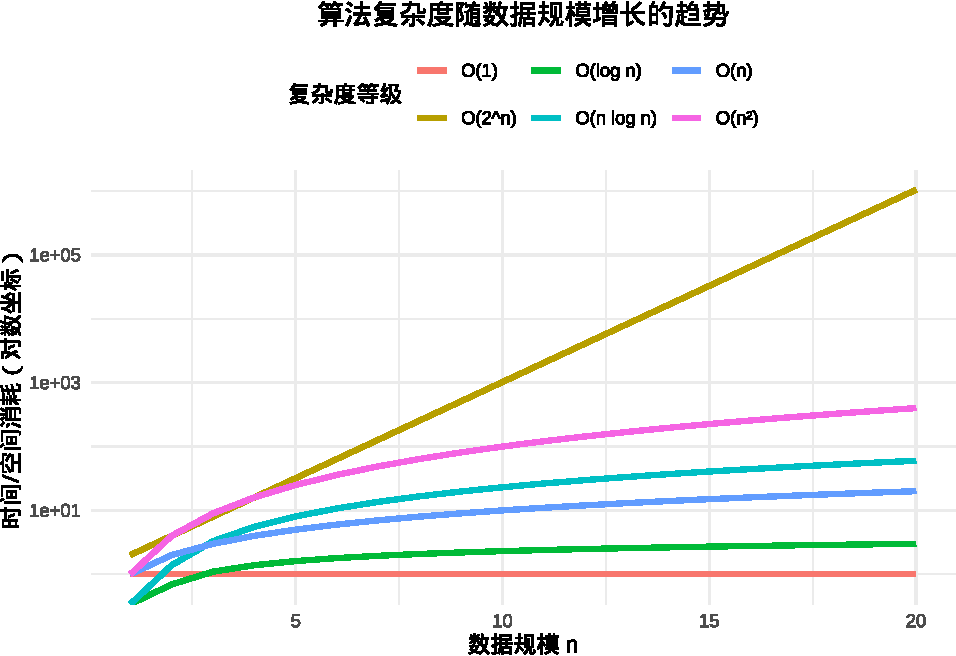
\includegraphics{01-statistical_programing_files/figure-latex/complexity-curve-1.pdf}
\caption{\label{fig:complexity-curve}算法复杂度随数据规模增长的趋势图}
\end{figure}

图\ref{fig:complexity-curve} 直观地展示了不同复杂度等级随数据规模增长的趋势。\textbf{结论}:O(1) 和 O(log n) 是极其高效的,O(n) 和 O(n log n) 是优秀的,O(n²) 在 n 较小时可以接受,而 O(2\^{}n) 和 O(n!) 应尽量避免。

\hypertarget{ux7ed9ux6570ux636eux5206ux6790ux5e08ux7684ux542fux793a}{%
\subsubsection{给数据分析师的启示}\label{ux7ed9ux6570ux636eux5206ux6790ux5e08ux7684ux542fux793a}}

\textbf{数据规模是关键}这一认知在生态学数据分析中具有决定性意义。当处理小规模数据集时,算法选择的差异可能并不明显------一个O(n²)的算法在几百条记录上运行可能只需要几毫秒。然而,当数据规模从1万条增长到100万条时,复杂度差异的威力就会充分显现。一个O(n²)的算法(如双重循环进行物种匹配)耗时将增加1万倍,从原本的1秒延长到近3小时;而一个O(n log n)的高效排序算法可能只增加不到20倍,从1秒延长到20秒左右。这种指数级的性能差异决定了某些分析方法在大数据场景下的可行性。在生态学研究中,这意味着我们需要根据预期的数据规模来前瞻性地选择分析方法,而不是等到数据积累到一定规模后再被动调整。

\textbf{理解R语言操作的代价}是生态学数据分析师的核心能力。许多看似简单的R操作背后都隐藏着复杂的算法实现。例如,\texttt{table()}函数用于统计物种频数,其时间复杂度通常是O(n),但当处理大规模数据时仍需注意内存使用;\texttt{merge()}函数进行数据框合并,其复杂度取决于合并策略,可能达到O(n log n)或更高;\texttt{sort()}函数的性能差异更为明显------R默认使用快速排序(平均O(n log n)),但在最坏情况下可能退化到O(n²)。理解这些操作的复杂度特征,能够帮助我们在设计分析流程时做出明智的决策。比如,在处理大型物种分布矩阵时,应该避免在循环内部重复调用\texttt{table()},而是应该预先计算好统计结果。

\textbf{空间换时间}是数据分析中经典的优化策略,在生态学研究中尤为实用。这种策略的核心思想是利用额外的内存存储来避免重复计算,从而显著降低时间复杂度。一个典型的例子是物种多样性分析:如果我们使用双重循环计算所有物种对之间的共存关系,时间复杂度为O(n²);但如果我们先构建一个哈希表(在R中可以使用命名向量或环境对象)存储每个物种的分布信息,然后通过单次遍历完成计算,时间复杂度可以降低到O(n)。虽然这会增加O(n)的空间复杂度,但在现代计算机内存充足的情况下,这种权衡通常是值得的。另一个例子是生态位模型预测:通过预先计算和缓存环境变量的响应曲线,可以避免在预测阶段重复进行复杂的数学运算,从而大幅提升模型运行效率。这种优化思维不仅适用于编程实现,也适用于分析流程设计------通过合理的数据预处理和中间结果存储,我们可以构建既高效又可靠的大规模生态数据分析系统。

\textbf{练习}:尝试分析你写过的一些数据处理脚本,找出其中循环和操作,估算其时间复杂度和空间复杂度。这将极大地提升你的代码质量和性能优化能力。

\hypertarget{aiux534fux540cux7f16ux7a0bux6280ux80fd}{%
\section{AI协同编程技能}\label{aiux534fux540cux7f16ux7a0bux6280ux80fd}}

\hypertarget{aiux7f16ux7a0bux6a21ux5757ux5b89ux88c5}{%
\subsection{AI编程模块安装}\label{aiux7f16ux7a0bux6a21ux5757ux5b89ux88c5}}

大语言模型辅助编程(AI-assisted programming)是当前最热门的AI技术之一,它通过大规模预训练语言模型(如GPT-4、Claude、Qwen等)来协助程序员编写代码。这种技术革命性地改变了编程工作的本质,将程序员从繁琐的语法记忆和重复性编码任务中解放出来,使其能够更专注于算法设计、系统架构和问题解决等高层次思维活动。

然而,大模型训练和调用都需要大量计算资源,这使得AI协作编程的可行性在早期受到限制。直到2025年初DeepSeek等开源模型的出现,普通人AI协作编程的可行性才得到极大提升。随后这种AI辅助编程工具呈现爆发式增长,从最初的GitHub Copilot、DeepSeek,到后来的Claude Code、Codex、Cursor等,几乎每隔几天就有新的工具问世。这种快速迭代反映了AI技术在编程领域的巨大潜力和激烈竞争。

当前AI协作编程工具的种类已经非常丰富,涵盖了从代码补全、错误修复、代码重构到完整功能实现的各个层面。但技术的快速演进也意味着任何具体工具的详细介绍都可能很快过时。因此,本章不追求对特定工具的详尽介绍,而是聚焦于通用的AI协作编程思维框架和核心技能培养。无论使用哪种具体工具,研究者都需要掌握精确提问、代码审查、迭代优化等基本能力。

作为代表性工具,Qwen Code是一个基于大模型的AI协作编程工具,它借鉴了Claude Code的设计理念,支持通过Qwen Coder或Claude Code等大模型来协助编程工作。Qwen Code的特点包括命令行工作流设计、OAuth一键登录、会话管理等功能,为生态学研究者提供了便捷的AI编程协作体验。但更重要的是,通过学习和使用这类工具,研究者能够建立起与AI有效协作的思维模式,这种能力将超越具体工具的局限,成为AI时代生态学数据分析的核心竞争力。

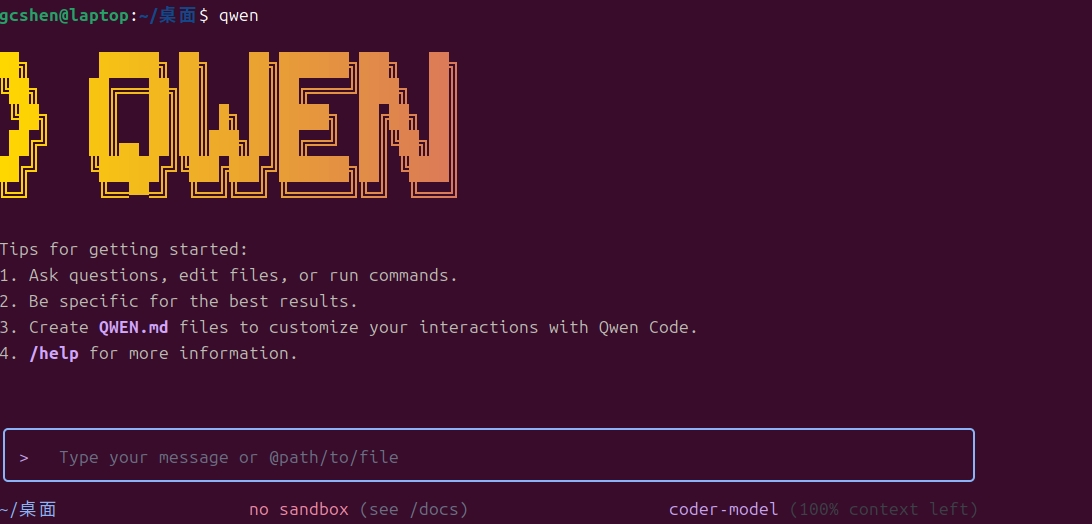
\includegraphics{imgs/qwen-code.jpg}

Qwen Code(阿里通义:\textbf{qwen} 命令的 CLI)

\begin{quote}
明确对标 Claude Code 的命令行工作流工具,对 \textbf{Qwen3-Coder} 优化;支持 \textbf{OAuth 一键登录}(国际/国内均有渠道),也支持 OpenAI-兼容 API;提供 \texttt{/compress}、\texttt{/stats} 等会话管理命令。({[}GitHub{]}{[}8{]})
\end{quote}

\textbf{安装}

\begin{Shaded}
\begin{Highlighting}[]
\CommentTok{\# 需 Node.js 20+}
\ExtensionTok{npm}\NormalTok{ install }\AttributeTok{{-}g}\NormalTok{ @qwen{-}code/qwen{-}code@latest}
\ExtensionTok{qwen} \AttributeTok{{-}{-}version}
\CommentTok{\# 或 Homebrew(macOS/Linux)}
\ExtensionTok{brew}\NormalTok{ install qwen{-}code}
\end{Highlighting}
\end{Shaded}

({[}GitHub{]}{[}8{]})

\textbf{登录(两种模式)}

\begin{Shaded}
\begin{Highlighting}[]
\CommentTok{\# 方式1:Qwen OAuth(零配置,推荐)}
\ExtensionTok{qwen}    \CommentTok{\# 会自动弹浏览器登录 qwen.ai 账户并缓存凭证}

\CommentTok{\# 方式2:OpenAI 兼容 API(适合私有部署/跨地区)}
\BuiltInTok{export} \VariableTok{OPENAI\_API\_KEY}\OperatorTok{=}\NormalTok{...}
\BuiltInTok{export} \VariableTok{OPENAI\_BASE\_URL}\OperatorTok{=}\NormalTok{...    }\CommentTok{\# 例:DashScope/ModelScope/OpenRouter}
\BuiltInTok{export} \VariableTok{OPENAI\_MODEL}\OperatorTok{=}\NormalTok{qwen3{-}coder{-}plus}
\end{Highlighting}
\end{Shaded}

\textbf{上手 \& 常用命令}

\begin{Shaded}
\begin{Highlighting}[]
\BuiltInTok{cd}\NormalTok{ your{-}project}
\ExtensionTok{qwen}
\CommentTok{\# 交互里可以直接自然语言:}
\OperatorTok{\textgreater{}}\NormalTok{ Explain }\ExtensionTok{the}\NormalTok{ codebase structure}
\OperatorTok{\textgreater{}}\NormalTok{ Refactor }\ExtensionTok{this}\NormalTok{ function}
\OperatorTok{\textgreater{}}\NormalTok{ Generate }\ExtensionTok{unit}\NormalTok{ tests}

\CommentTok{\# 会话管理}
\ExtensionTok{/clear}\NormalTok{   /compress   /stats   /exit}
\end{Highlighting}
\end{Shaded}

\textbf{VS Code中集成}

在插件市场吗,搜索 \textbf{Qwen Code} 安装即可。

\hypertarget{ux7cbeux51c6ux63d0ux95eeux6280ux5de7}{%
\subsection{精准提问技巧}\label{ux7cbeux51c6ux63d0ux95eeux6280ux5de7}}

\hypertarget{promptux5de5ux7a0bux57faux672cux539fux5219}{%
\subsubsection{Prompt工程基本原则}\label{promptux5de5ux7a0bux57faux672cux539fux5219}}

\textbf{生态学数据分析的Prompt示例}:

\begin{verbatim}
请用R语言帮我分析森林样地数据:

数据描述:
- 数据框包含以下列:plot_id(样地编号)、species(物种名称)、dbh(胸径)、height(树高)
- 数据已保存在CSV文件中,路径为"data/forest_survey.csv"

分析要求:
1. 读取数据并检查数据质量(缺失值、异常值)
2. 计算每个样地的物种丰富度(物种数)
3. 计算每个样地的平均胸径和平均树高
4. 绘制物种丰富度与平均胸径的关系散点图
5. 使用ggplot2进行可视化,添加适当的标题和标签

请为关键步骤添加注释,并确保代码具有良好的可读性。
\end{verbatim}

\hypertarget{ux4e0aux4e0bux6587ux63d0ux4f9bux4e0eux7ea6ux675fux6761ux4ef6ux8bbeux5b9a}{%
\subsubsection{上下文提供与约束条件设定}\label{ux4e0aux4e0bux6587ux63d0ux4f9bux4e0eux7ea6ux675fux6761ux4ef6ux8bbeux5b9a}}

\textbf{改进的Prompt示例}:

\begin{verbatim}
我正在分析天童森林动态监测样地的数据,需要计算生物多样性指数。

约束条件:
- 数据包含200个固定样地的调查结果
- 每个样地面积为20m×20m
- 只统计DBH≥1cm的木本植物
- 需要排除外来物种和栽培物种

具体要求:
1. 计算每个样地的Shannon-Wiener多样性指数
2. 计算每个样地的Simpson多样性指数
3. 分析多样性指数与海拔的相关性
4. 生成专业的研究报告图表

请使用vegan包进行多样性计算,确保代码符合生态学研究的标准做法。
\end{verbatim}

\hypertarget{ux4ee3ux7801ux5ba1ux67e5ux80fdux529b}{%
\subsection{代码审查能力}\label{ux4ee3ux7801ux5ba1ux67e5ux80fdux529b}}

\hypertarget{llmux8f93ux51faux4ee3ux7801ux7684ux5e38ux89c1ux9519ux8befux7c7bux578b}{%
\subsubsection{LLM输出代码的常见错误类型}\label{llmux8f93ux51faux4ee3ux7801ux7684ux5e38ux89c1ux9519ux8befux7c7bux578b}}

\begin{Shaded}
\begin{Highlighting}[]
\CommentTok{\# LLM可能生成的有问题的代码示例}
\CommentTok{\# 问题1:缺乏错误处理}
\NormalTok{calculate\_density }\OtherTok{\textless{}{-}} \ControlFlowTok{function}\NormalTok{(area, count) \{}
\NormalTok{  density }\OtherTok{\textless{}{-}}\NormalTok{ count }\SpecialCharTok{/}\NormalTok{ area }\CommentTok{\# 如果area为0会出错}
  \FunctionTok{return}\NormalTok{(density)}
\NormalTok{\}}

\CommentTok{\# 改进版本}
\NormalTok{calculate\_density\_safe }\OtherTok{\textless{}{-}} \ControlFlowTok{function}\NormalTok{(area, count) \{}
  \ControlFlowTok{if}\NormalTok{ (area }\SpecialCharTok{\textless{}=} \DecValTok{0}\NormalTok{) \{}
    \FunctionTok{stop}\NormalTok{(}\StringTok{"面积必须大于0"}\NormalTok{)}
\NormalTok{  \}}
\NormalTok{  density }\OtherTok{\textless{}{-}}\NormalTok{ count }\SpecialCharTok{/}\NormalTok{ area}
  \FunctionTok{return}\NormalTok{(density)}
\NormalTok{\}}

\CommentTok{\# 问题2:使用过时的函数}
\CommentTok{\# LLM可能推荐使用旧的函数版本}

\CommentTok{\# 改进:使用更现代的tidyverse方法}
\FunctionTok{library}\NormalTok{(tidyverse)}
\end{Highlighting}
\end{Shaded}

\begin{verbatim}
## -- Attaching core tidyverse packages --------------------------------------------------------------------------------------------------------- tidyverse 2.0.0 --
## v forcats   1.0.0     v readr     2.1.5
## v lubridate 1.9.4     v tibble    3.2.1
## v purrr     1.1.0     v tidyr     1.3.1
## -- Conflicts --------------------------------------------------------------------------------------------------------------------------- tidyverse_conflicts() --
## x readr::edition_get()   masks testthat::edition_get()
## x dplyr::filter()        masks stats::filter()
## x purrr::is_null()       masks testthat::is_null()
## x dplyr::lag()           masks stats::lag()
## x readr::local_edition() masks testthat::local_edition()
## x tidyr::matches()       masks testthat::matches(), dplyr::matches()
## i Use the conflicted package (<http://conflicted.r-lib.org/>) to force all conflicts to become errors
\end{verbatim}

\hypertarget{ux529fux80fdux6b63ux786eux6027ux9a8cux8bc1ux65b9ux6cd5}{%
\subsubsection{功能正确性验证方法}\label{ux529fux80fdux6b63ux786eux6027ux9a8cux8bc1ux65b9ux6cd5}}

\begin{Shaded}
\begin{Highlighting}[]
\CommentTok{\# 创建测试用例验证函数正确性}
\NormalTok{test\_diversity\_calculation }\OtherTok{\textless{}{-}} \ControlFlowTok{function}\NormalTok{() \{}
  \CommentTok{\# 测试用例1:单一物种}
\NormalTok{  single\_species }\OtherTok{\textless{}{-}} \FunctionTok{rep}\NormalTok{(}\StringTok{"Oak"}\NormalTok{, }\DecValTok{10}\NormalTok{)}
\NormalTok{  result1 }\OtherTok{\textless{}{-}} \FunctionTok{calculate\_diversity}\NormalTok{(single\_species)}

  \CommentTok{\# 单一物种的Shannon指数应该为0}
  \ControlFlowTok{if}\NormalTok{ (}\FunctionTok{abs}\NormalTok{(result1 }\SpecialCharTok{{-}} \DecValTok{0}\NormalTok{) }\SpecialCharTok{\textgreater{}} \FloatTok{1e{-}10}\NormalTok{) \{}
    \FunctionTok{stop}\NormalTok{(}\StringTok{"单一物种测试失败"}\NormalTok{)}
\NormalTok{  \}}

  \CommentTok{\# 测试用例2:两个物种各占一半}
\NormalTok{  two\_species }\OtherTok{\textless{}{-}} \FunctionTok{rep}\NormalTok{(}\FunctionTok{c}\NormalTok{(}\StringTok{"Oak"}\NormalTok{, }\StringTok{"Pine"}\NormalTok{), }\AttributeTok{each =} \DecValTok{5}\NormalTok{)}
\NormalTok{  result2 }\OtherTok{\textless{}{-}} \FunctionTok{calculate\_diversity}\NormalTok{(two\_species)}

  \CommentTok{\# 两个物种各占一半的Shannon指数应该为log(2)}
\NormalTok{  expected }\OtherTok{\textless{}{-}} \FunctionTok{log}\NormalTok{(}\DecValTok{2}\NormalTok{)}
  \ControlFlowTok{if}\NormalTok{ (}\FunctionTok{abs}\NormalTok{(result2 }\SpecialCharTok{{-}}\NormalTok{ expected) }\SpecialCharTok{\textgreater{}} \FloatTok{1e{-}10}\NormalTok{) \{}
    \FunctionTok{stop}\NormalTok{(}\StringTok{"两个物种测试失败"}\NormalTok{)}
\NormalTok{  \}}

  \FunctionTok{cat}\NormalTok{(}\StringTok{"所有测试通过!}\SpecialCharTok{\textbackslash{}n}\StringTok{"}\NormalTok{)}
\NormalTok{\}}

\CommentTok{\# 运行测试}
\FunctionTok{test\_diversity\_calculation}\NormalTok{()}
\end{Highlighting}
\end{Shaded}

\begin{verbatim}
## 所有测试通过!
\end{verbatim}

\hypertarget{ux8c03ux8bd5ux4e0eux9519ux8befux5904ux7406}{%
\subsection{调试与错误处理}\label{ux8c03ux8bd5ux4e0eux9519ux8befux5904ux7406}}

\hypertarget{ux9519ux8befux4fe1ux606fux89e3ux8bfbux4e0eux5b9aux4f4d}{%
\subsubsection{错误信息解读与定位}\label{ux9519ux8befux4fe1ux606fux89e3ux8bfbux4e0eux5b9aux4f4d}}

\begin{Shaded}
\begin{Highlighting}[]
\CommentTok{\# 常见的R错误信息及解决方法}

\CommentTok{\# 错误1:对象未找到}
\CommentTok{\# Error: object \textquotesingle{}x\textquotesingle{} not found}
\CommentTok{\# 解决方法:检查变量名拼写,确保变量已赋值}

\CommentTok{\# 错误2:函数参数不匹配}
\CommentTok{\# Error in mean(x) : 参数不是数值也不是逻辑值:回传NA}
\CommentTok{\# 解决方法:检查数据类型,确保输入是数值型}

\CommentTok{\# 错误3:下标越界}
\CommentTok{\# Error in x[5] : 下标出界}
\CommentTok{\# 解决方法:检查向量长度,确保索引在有效范围内}

\CommentTok{\# 实用的调试技巧}
\NormalTok{debug\_calculation }\OtherTok{\textless{}{-}} \ControlFlowTok{function}\NormalTok{(data) \{}
  \CommentTok{\# 使用browser()进行交互式调试}
  \FunctionTok{browser}\NormalTok{()}

\NormalTok{  result }\OtherTok{\textless{}{-}} \FunctionTok{calculate\_diversity}\NormalTok{(data)}
  \FunctionTok{return}\NormalTok{(result)}
\NormalTok{\}}

\CommentTok{\# 使用tryCatch处理错误}
\NormalTok{safe\_calculation }\OtherTok{\textless{}{-}} \ControlFlowTok{function}\NormalTok{(data) \{}
\NormalTok{  result }\OtherTok{\textless{}{-}} \FunctionTok{tryCatch}\NormalTok{(}
\NormalTok{    \{}
      \CommentTok{\# 尝试执行可能出错的操作}
      \FunctionTok{calculate\_diversity}\NormalTok{(data)}
\NormalTok{    \},}
    \AttributeTok{error =} \ControlFlowTok{function}\NormalTok{(e) \{}
      \CommentTok{\# 错误处理}
      \FunctionTok{cat}\NormalTok{(}\StringTok{"计算失败:"}\NormalTok{, e}\SpecialCharTok{$}\NormalTok{message, }\StringTok{"}\SpecialCharTok{\textbackslash{}n}\StringTok{"}\NormalTok{)}
      \FunctionTok{return}\NormalTok{(}\ConstantTok{NULL}\NormalTok{)}
\NormalTok{    \},}
    \AttributeTok{warning =} \ControlFlowTok{function}\NormalTok{(w) \{}
      \CommentTok{\# 警告处理}
      \FunctionTok{cat}\NormalTok{(}\StringTok{"警告:"}\NormalTok{, w}\SpecialCharTok{$}\NormalTok{message, }\StringTok{"}\SpecialCharTok{\textbackslash{}n}\StringTok{"}\NormalTok{)}
      \FunctionTok{return}\NormalTok{(}\FunctionTok{calculate\_diversity}\NormalTok{(data)) }\CommentTok{\# 继续执行}
\NormalTok{    \}}
\NormalTok{  )}

  \FunctionTok{return}\NormalTok{(result)}
\NormalTok{\}}
\end{Highlighting}
\end{Shaded}

\hypertarget{ux603bux7ed3}{%
\section{总结}\label{ux603bux7ed3}}

本章系统性地构建了AI时代生态学统计编程的全新教育框架,标志着编程教育从''技能导向''向''思维导向''的根本性转变。在大语言模型成为强大编程助手的今天,编程教育的核心价值已不再体现在语法记忆和API细节掌握上,而是转向更高层次的思维能力培养。

本章重点培养了两大核心能力体系:首先是\textbf{高阶思维与问题解决能力},包括问题分解与抽象建模能力、算法与数据结构思维、数据分析流程设计与规划能力。这些能力构成了生态学研究者驾驭AI工具的''方向盘'',确保研究者能够站在战略高度设计分析方案,而不仅仅是执行具体的编程任务。其次是\textbf{与LLM协同工作的能力},涵盖精确提问与Prompt工程、代码审查与批判性验证、迭代与优化等关键技能,这些能力使研究者能够有效指导AI完成复杂的数据分析任务。

在技术层面,本章通过模块化的学习路径,系统介绍了通用编程思维基础,包括变量与常量、数据类型、运算符、集合数据类型、分支与循环、函数、作用域、错误处理、模块化、面向对象、内存管理、测试和代码规范等核心概念。这些知识为生态学数据分析提供了坚实的技术基础,确保研究者能够理解计算的基本原理,而不仅仅是记忆特定工具的使用方法。

特别值得强调的是,本章提出的''分析方案设计师 + AI指令员 + 质量保证官''三位一体的角色定位,精准地捕捉了AI时代生态学研究者的核心竞争力。研究者不再需要为琐碎的编程细节所困扰,而是将精力集中在更具价值的分析设计、方法选择和结果解释上。这种角色转变不仅提高了研究效率,更提升了研究的科学性和创新性。

通过本章的学习,学生将建立起现代数据分析的思维框架,能够将复杂的生态学问题转化为清晰可执行的分析流程,并利用AI工具高效实现技术方案。这种能力框架具有高度的通用性和适应性,不仅适用于当前的R语言生态,也为未来学习其他编程语言和分析工具奠定了坚实基础。

在后续章节中,我们将基于本章建立的编程思维框架,深入探讨更专业的生态统计方法。但无论技术工具如何发展,本章所强调的分析思维、问题解决能力和AI协作素养,都将成为生态学研究者应对技术变革、推动学科发展的核心竞争优势。这种以思维为导向的编程教育,正是培养未来生态学创新人才的关键路径。

\hypertarget{ux7efcux5408ux7ec3ux4e60}{%
\section{综合练习}\label{ux7efcux5408ux7ec3ux4e60}}

\hypertarget{ux7ec3ux4e601}{%
\subsection{练习1}\label{ux7ec3ux4e601}}

请在AI的协助下,判断项目data目录下的Tiantong\_Sample.CSV文件内的所有树木空间位置是否是随机分布?请注意,写完代码和出了结果后,并不代表该习题的结束。你需要在AI的协助下,理解其分析思路,每行代码的意思。下堂课会随机请人上来讲解。

\hypertarget{ux6982ux7387ux4e0eux5206ux5e03}{%
\chapter{概率与分布}\label{ux6982ux7387ux4e0eux5206ux5e03}}

\hypertarget{ux5f15ux8a00-1}{%
\section{引言}\label{ux5f15ux8a00-1}}

当人工智能的浪潮如春风般拂过科学研究的每一片田野,生态学专业的学生心中或许会浮现这样的疑问:在AI能够驾驭海量数据、揭示复杂模式的今天,我们为何还要深入理解概率与分布这些看似基础的数学概念?难道强大的AI不能为我们处理所有的数据分析任务吗?

要回答这个深刻的问题,我们需要洞察AI工具与数学理论之间的本质关系。AI系统如同威力巨大的数据分析引擎,能够驾驭信息海洋并揭示复杂模式,但其输出的本质始终是概率性的。当我们使用AI模型预测物种分布、评估生态风险或分析气候变化影响时,模型给出的结果永远伴随着不确定性的阴影。如果不理解这些不确定性背后的概率原理,我们就如同盲人摸象,无法正确解读AI的输出,也无法评估模型的可信度。

概率理论如同我们理解AI''黑箱''的钥匙,帮助我们解读模型输出的深层含义------AI给出的''预测概率''究竟代表什么,95\%的置信区间应该如何正确理解。同时,概率知识如同生态学家的指南针,指引我们设计有效的采样方案,理解适合训练AI模型的数据分布特征,并巧妙避开采样偏差的陷阱。更重要的是,概率理论为模型比较和选择提供了科学依据,帮助我们判断不同AI模型之间的性能差异是否具有统计显著性。

生态学研究面对的是自然界中最为复杂的系统之一。与物理实验不同,生态学观察往往无法在完全控制的条件下重复进行。从蚱蜢的午餐选择到树木的生长模式,从种群动态变化到生态系统功能,这些现象都充满了随机性和不确定性。概率与分布理论为我们提供了量化这种不确定性的数学语言,如同在混沌的自然世界中点亮了一盏明灯。

生态学数据具有独特的复杂性特征。空间异质性意味着物种在不同生境中的分布模式存在差异;时间依赖性表明生态过程具有记忆效应;多重尺度特性要求我们理解从个体到生态系统不同层次的概率规律;稀有事件如物种灭绝、极端气候虽然发生概率小,却具有重大生态意义。这些特征使得简单的统计方法往往失效,需要基于深刻概率理解的复杂模型。

在AI时代,仅仅掌握现成分析工具是不够的。真正的生态学家需要具备批判性思考能力,能够质疑AI模型的假设和局限性;需要创造性建模能力,针对特定生态问题设计合适的概率模型;需要跨学科整合能力,将概率理论与生态学知识、计算技术有机结合;还需要不确定性沟通能力,向决策者和公众清晰传达研究结果的不确定性。概率与分布理论正是培养这些能力的基础,教会我们如何思考不确定性、量化随机性、从噪声中提取信号。

通过本章的学习,你将不仅掌握概率与分布的基本概念,更重要的是培养''概率思维''------用数学语言描述和理解生态世界的能力。这种能力如同生态学家的超级直觉,使你能够设计合理的生态调查方案,正确解读复杂的生态数据,与数据科学家有效合作,并在AI时代保持批判性和创造性。

在AI辅助研究的时代,最宝贵的不是知道如何使用工具,而是理解工具背后的原理。概率与分布理论就是这样的基本原理,它们连接生态观察与数学分析,为我们在数据海洋中提供导航工具。让我们开始这段探索之旅,从蚱蜢的午餐选择出发,逐步构建理解生态世界不确定性的数学框架。

\hypertarget{ux8682ux86b1ux5348ux9910ux4e0eux6982ux7387}{%
\section{蚂蚱午餐与概率}\label{ux8682ux86b1ux5348ux9910ux4e0eux6982ux7387}}

\hypertarget{ux4e00ux53eaux86b1ux8722ux7684ux5348ux9910}{%
\subsection{一只蚱蜢的午餐}\label{ux4e00ux53eaux86b1ux8722ux7684ux5348ux9910}}

想象校园里一只普通的蚱蜢,它站在生命的十字路口,面前是三片风格迥异的草地:茂盛的黑麦草如同营养丰富的盛宴,点缀雏菊的混合草甸宛如充满惊喜的冒险乐园,以三叶草为主的区域则像是一片等待探索的神秘领地。对蚱蜢而言,这些不仅仅是风景,而是它生命中每一次选择的机会,是它''餐桌''上的命运抉择。

这个看似简单的问题背后,隐藏着生态学研究的核心挑战:蚱蜢下一顿午餐会选择在哪一种植物上进食?这个问题如同生态学中的''薛定谔的猫'',在观察之前,答案永远处于不确定的叠加状态。

蚱蜢的选择受到多重因素的微妙影响:黑麦草的营养价值如同理性的召唤,混合草甸的隐蔽性如同安全的诱惑,三叶草的口感则像是味蕾的邀请。天气的变幻、饥饿的程度、捕食者的阴影,这些变量如同命运之手中的骰子,每一次滚动都可能改变最终的结局。

作为生态学研究者,我们的使命是量化这种''选择偏好'',将模糊的生物直觉转化为精确的数学语言。这种偏好本质上就是\textbf{概率}------介于0和1之间的数字,如同自然界中的魔法数字,描述不确定事件(蚱蜢选择某种植物)发生的可能性。概率为0表示绝不可能,如同永远不会发生的奇迹;概率为1表示必然发生,如同日升月落的自然规律。现实世界中的概率通常介于这两个极端之间,如同生命本身,充满了复杂性和随机性的美丽。

如何度量和理解蚱蜢的''选择概率''?这不仅是简单的计数问题,而是需要建立数学模型来描述行为模式,如同用数学语言谱写生命的乐章。概率理论为我们提供了三种不同视角来理解这种不确定性:基于理想假设的古典概率如同数学家的完美梦想,基于实际观察的频率概率如同科学家的严谨实验,能够结合新证据更新认知的贝叶斯概率则如同哲学家不断进化的智慧。每种方法都有其独特的价值和适用场景,共同构成我们理解自然界的数学工具箱,如同三把不同形状的钥匙,共同开启生态世界不确定性的大门。

\hypertarget{ux7406ux60f3ux7684ux731cux6d4bux53e4ux5178ux6982ux7387}{%
\subsection{理想的猜测------古典概率}\label{ux7406ux60f3ux7684ux731cux6d4bux53e4ux5178ux6982ux7387}}

在缺乏观察数据的迷雾中,我们基于''公平原则''进行理想化的猜测。想象蚱蜢活动区域内黑麦草、混合草甸和三叶草的面积相等,如同命运天平上的三个等重砝码,那么选择任何一种植物的可能性应该完全相同。

\textbf{这就是古典概率(先验概率)},其核心是''等可能性''的优雅假设。在这个理想化的数学花园中,三种可能结果如同三朵同样鲜艳的花朵,绽放的可能性完全相同。\textbf{计算公式为:} \[P(\text{蚱蜢选择黑麦草}) = \frac{\text{有利于该事件的结果数}}{\text{所有可能的结果数}} = \frac{1}{3}\] 这种概率源于逻辑推理的纯粹之美而非实际数据的复杂现实,简洁优美但现实世界往往不如此''公平''。蚱蜢可能对某种植物有特殊偏好,如同每个人心中都有自己偏爱的风景。

\hypertarget{ux6838ux5fc3ux601dux60f3ux7b49ux53efux80fdux6027}{%
\subsubsection{核心思想:等可能性}\label{ux6838ux5fc3ux601dux60f3ux7b49ux53efux80fdux6027}}

考虑一个完全公平的掷骰子游戏,骰子质地均匀、形状完美。在掷出之前,掷出''1点''的可能性是多少?直觉告诉我们:六分之一。

支撑这个直觉的是古典概率(先验概率)的思维方式。这是概率论中最古老、最直观的定义,源于对机会游戏的研究。古典概率的历史可追溯到17世纪,法国数学家布莱兹·帕斯卡和皮埃尔·德·费马通过书信往来解决了赌博概率问题,为现代概率论奠定了基础。

古典概率的核心前提是''等可能性''------随机试验的所有可能结果发生的可能性完全相同。这个假设看似简单,却蕴含深刻的数学哲学思想。等可能性建立在对称性原则之上:当我们说骰子六个面''等可能''时,实际上指骰子在几何形状、质量分布等方面具有完美对称性,确保每个面朝上的物理条件完全相同。

在生态学中,等可能性假设意味着暂时忽略所有可能影响生物选择的因素,将系统简化为完全随机过程。这种简化虽不完美,但提供了理论基准,帮助我们理解''如果世界完全随机会发生什么''。

\hypertarget{ux5b9aux4e49ux4e0eux516cux5f0f}{%
\subsubsection{定义与公式}\label{ux5b9aux4e49ux4e0eux516cux5f0f}}

在满足``等可能性''的试验中,我们称每个单一的可能结果为一个 ``\textbf{基本事件}'' 。所有基本事件构成的集合,就是 ``\textbf{样本空间}''。样本空间的概念是概率论的基础,它定义了所有可能发生的结果。

构建样本空间需要仔细考虑试验的所有可能结果。例如,在蚱蜢选择植物的例子中,样本空间包含三个基本事件:\{选择黑麦草,选择混合草甸,选择三叶草\}。每个基本事件都是互斥且完备的------互斥意味着不可能同时发生两个事件,完备意味着涵盖了所有可能性。

古典概率的定义公式简洁而优美:

\[P(A) = \frac{\text{事件A包含的基本事件个数}}{\text{样本空间中基本事件的总数}}\]

\(P(A)\): 事件A发生的概率。分子: 你关心的事件A包含了多少种可能的结果。分母: 整个试验一共有多少种可能的结果。

这个公式计算出的概率,是一个介于0和1之间的数。\(P(A)=0\)表示事件A不可能发生;\(P(A)=1\)表示事件A必然发生。概率的归一化条件要求所有基本事件的概率之和等于1。

\hypertarget{ux6982ux7387ux7684ux4e09ux4e2aux57faux672cux5c5eux6027}{%
\subsubsection{概率的三个基本属性}\label{ux6982ux7387ux7684ux4e09ux4e2aux57faux672cux5c5eux6027}}

无论采用哪种概率定义(古典、频率或贝叶斯),概率都必须满足三个基本公理,这些公理由俄罗斯数学家安德雷·柯尔莫哥洛夫在1933年提出,为现代概率论奠定了坚实的数学基础。

\textbf{公理1:非负性}
对于任意事件A,其概率总是非负的:
\[P(A) \geq 0\]

这个公理确保了概率的合理性。在生态学中,这意味着任何生态事件的发生概率都不可能为负值,无论这个事件多么罕见或不可能。

\textbf{公理2:规范性}
整个样本空间的概率为1:
\[P(\Omega) = 1\]

其中\(\Omega\)表示样本空间,即所有可能结果的集合。这个公理表明''必然事件''的概率为1。在蚱蜢的例子中,样本空间包含三种植物选择,因此\(P(\text{选择任意植物}) = 1\)。

\textbf{公理3:可加性}
对于任意两个互斥事件A和B(即A和B不能同时发生):
\[P(A \cup B) = P(A) + P(B)\]

这个公理可以推广到有限个或可数无限个互斥事件。在生态学中,这意味着如果两个生态事件不可能同时发生(如''蚱蜢同时选择黑麦草和混合草甸''),那么它们中至少有一个发生的概率等于各自概率之和。

这三个公理共同构成了概率论的数学基础,确保了概率计算的逻辑一致性。从这些基本公理出发,我们可以推导出概率的所有其他性质,如:
- \(P(A^c) = 1 - P(A)\)(互补事件的概率)
- 如果\(A \subseteq B\),则\(P(A) \leq P(B)\)(概率的单调性)
- \(P(A \cup B) = P(A) + P(B) - P(A \cap B)\)(一般加法公式)

这些性质在生态学研究中具有重要的应用价值,帮助我们建立合理的概率模型并进行正确的统计推断。

\hypertarget{ux751fux6001ux5b66ux4e2dux7684ux53e4ux5178ux6982ux7387ux5e94ux7528}{%
\subsubsection{生态学中的古典概率应用}\label{ux751fux6001ux5b66ux4e2dux7684ux53e4ux5178ux6982ux7387ux5e94ux7528}}

尽管古典概率的假设很强,但在某些生态学场景中仍然有其应用价值。首先,在\textbf{理想化的种群分布模型}中,当我们研究物种在栖息地中的分布时,可以先建立一个''等可能性''的基准模型。例如,假设一个森林中有三种不同类型的微生境(阳光充足区、半阴区、全阴区),我们可以先假设物种在这三种生境中出现的概率相等,然后与实际观测数据进行比较。这种比较可以帮助我们识别物种的真实偏好。

其次,在\textbf{随机抽样设计}方面,生态调查中经常需要随机选择样方位置。如果样方选择过程真正实现了''等可能性'',那么每个位置被选中的概率应该完全相同。这种设计确保了样本的代表性,避免了选择偏差。

最后,在\textbf{遗传学中的孟德尔定律}应用中,种群遗传学中的孟德尔遗传定律实际上就是基于古典概率的等可能性假设。当亲本的基因型确定后,子代获得特定基因组合的概率可以通过古典概率计算。

\hypertarget{ux53e4ux5178ux6982ux7387ux7684ux5c40ux9650ux6027}{%
\subsubsection{古典概率的局限性}\label{ux53e4ux5178ux6982ux7387ux7684ux5c40ux9650ux6027}}

尽管古典概率模型非常优美,但它的''理想化''也恰恰是它在现实应用中的主要局限。古典概率的第一个显著局限在于\textbf{``等可能性''假设过于苛刻}。现实世界中,很多情况不满足等可能性假设,生态系统的复杂性使得这种假设往往过于简化。回到蚱蜢的例子,我们很难断言蚱蜢选择黑麦草、混合草甸和三叶草的可能性完全相等。植物的营养价值、口感、防御性化学物质、空间分布、季节变化等因素都存在差异,这些都会破坏''等可能性''假设。同样,一枚实际硬币可能因工艺瑕疵导致正面和反面出现的概率并非精确的50\%,研究表明大多数硬币实际上有51\%-49\%的轻微偏差。一只青蛙选择池塘时,池塘的大小、水深、水质、是否有天敌、食物丰富度等因素必然会影响其选择,使得''等可能性''的假设难以成立。

古典概率的第二个局限是\textbf{样本空间必须是有限集合}。古典概率要求可能的结果是有限可数的,对于连续性问题(如蚱蜢的精确跳跃距离是1.253米),因为结果有无限多个,古典概率便无能为力。生态学中的许多测量值都是连续变量,如温度、湿度、生物量等,这些都需要连续概率分布来描述。古典概率还要求明确知道总体大小,但生态学中总体往往无限或未知:

\begin{Shaded}
\begin{Highlighting}[]
\CommentTok{\# 有限总体问题示例:估计森林中濒危物种的数量}
\CommentTok{\# 演示古典概率在现实生态学中的局限性}

\CommentTok{\# 设置随机种子确保结果可重现}
\FunctionTok{set.seed}\NormalTok{(}\DecValTok{222}\NormalTok{)}

\CommentTok{\# 定义真实参数(实际研究中未知)}
\NormalTok{true\_rare\_species }\OtherTok{\textless{}{-}} \DecValTok{15}  \CommentTok{\# 实际濒危物种数量}

\CommentTok{\# 模拟调查数据(存在抽样偏差)}
\NormalTok{observed\_species }\OtherTok{\textless{}{-}} \DecValTok{8}    \CommentTok{\# 调查发现的物种数量}
\NormalTok{survey\_effort }\OtherTok{\textless{}{-}} \DecValTok{50}      \CommentTok{\# 调查努力程度(样方数或观察次数)}

\CommentTok{\# 计算检测概率:观测到的物种数除以调查努力程度}
\NormalTok{detection\_prob }\OtherTok{\textless{}{-}}\NormalTok{ observed\_species }\SpecialCharTok{/}\NormalTok{ survey\_effort}

\CommentTok{\# 使用检测概率估计总体数量:观测数除以检测概率}
\NormalTok{estimated\_total }\OtherTok{\textless{}{-}}\NormalTok{ observed\_species }\SpecialCharTok{/}\NormalTok{ detection\_prob}

\CommentTok{\# 输出结果对比,展示古典概率估计的误差}
\FunctionTok{cat}\NormalTok{(}\StringTok{"实际濒危物种数量:"}\NormalTok{, true\_rare\_species, }\StringTok{"}\SpecialCharTok{\textbackslash{}n}\StringTok{"}\NormalTok{)}
\end{Highlighting}
\end{Shaded}

\begin{verbatim}
## 实际濒危物种数量: 15
\end{verbatim}

\begin{Shaded}
\begin{Highlighting}[]
\FunctionTok{cat}\NormalTok{(}\StringTok{"观测到的物种数量:"}\NormalTok{, observed\_species, }\StringTok{"}\SpecialCharTok{\textbackslash{}n}\StringTok{"}\NormalTok{)}
\end{Highlighting}
\end{Shaded}

\begin{verbatim}
## 观测到的物种数量: 8
\end{verbatim}

\begin{Shaded}
\begin{Highlighting}[]
\FunctionTok{cat}\NormalTok{(}\StringTok{"检测概率:"}\NormalTok{, }\FunctionTok{round}\NormalTok{(detection\_prob, }\DecValTok{3}\NormalTok{), }\StringTok{"}\SpecialCharTok{\textbackslash{}n}\StringTok{"}\NormalTok{)}
\end{Highlighting}
\end{Shaded}

\begin{verbatim}
## 检测概率: 0.16
\end{verbatim}

\begin{Shaded}
\begin{Highlighting}[]
\FunctionTok{cat}\NormalTok{(}\StringTok{"估计的物种总数:"}\NormalTok{, }\FunctionTok{round}\NormalTok{(estimated\_total, }\DecValTok{1}\NormalTok{), }\StringTok{"}\SpecialCharTok{\textbackslash{}n}\StringTok{"}\NormalTok{)}
\end{Highlighting}
\end{Shaded}

\begin{verbatim}
## 估计的物种总数: 50
\end{verbatim}

\begin{Shaded}
\begin{Highlighting}[]
\FunctionTok{cat}\NormalTok{(}\StringTok{"估计误差:"}\NormalTok{, }\FunctionTok{round}\NormalTok{(}\FunctionTok{abs}\NormalTok{(estimated\_total }\SpecialCharTok{{-}}\NormalTok{ true\_rare\_species), }\DecValTok{1}\NormalTok{), }\StringTok{"}\SpecialCharTok{\textbackslash{}n}\StringTok{"}\NormalTok{)}
\end{Highlighting}
\end{Shaded}

\begin{verbatim}
## 估计误差: 35
\end{verbatim}

古典概率的第三个局限是\textbf{无法处理主观概率}。古典概率是客观的,基于计数,但它无法处理如''我认为明天会下雨的可能性是70\%``这种基于个人知识、经验和信念的主观判断。在生态学预测中,专家意见和经验判断往往很重要,但这些主观因素无法用古典概率来量化。

古典概率假设每次试验都是独立的,但生物行为往往具有记忆性和学习能力。如果蚱蜢昨天在黑麦草上获得了丰富的营养,它今天更可能再次选择黑麦草。这种历史依赖性破坏了古典概率的独立性假设。

\hypertarget{ux4eceux53e4ux5178ux6982ux7387ux5230ux73b0ux4ee3ux6982ux7387ux8bba}{%
\subsubsection{从古典概率到现代概率论}\label{ux4eceux53e4ux5178ux6982ux7387ux5230ux73b0ux4ee3ux6982ux7387ux8bba}}

古典概率虽然简单,但它为现代概率论的发展奠定了基础。20世纪初,俄罗斯数学家安德雷·柯尔莫哥洛夫建立了概率论的公理化体系,将概率定义为满足特定性质的测度函数。这个公理化体系能够同时涵盖古典概率、几何概率和统计概率,为概率论提供了坚实的数学基础。

总结来说,古典概率如同几何学中的完美圆规和直尺,它描绘了一个规则、公平、易于理解的理想世界。它是我们概率之旅的起点,教会我们''计数''的重要性,培养了我们对随机现象的基本直觉。当我们告别这个理想世界,步入充满复杂性和不确定性的真实生态学领域时,频率概率和贝叶斯概率等更强大的工具便会接过接力棒,帮助我们更好地刻画那只真实蚱蜢的、受到多种因素影响的午餐选择。古典概率的价值不在于它的现实准确性,而在于它为我们的思维提供了一个清晰的起点和参照系。

\hypertarget{ux6570ux636eux7684ux8bedux8a00ux9891ux7387ux6982ux7387}{%
\subsection{数据的语言------频率概率}\label{ux6570ux636eux7684ux8bedux8a00ux9891ux7387ux6982ux7387}}

为了了解真相,我决定进行实地观察。我在一周里,每天中午记录你进食的位置,一共记录了70次选择。数据如下:45次在黑麦草上,20次在混合草甸上,5次在三叶草上。

\textbf{这时,我使用的是频率概率。} 它的核心思想是:一个事件发生的概率,等于它在长期重复试验中出现的\textbf{频率}。\textbf{度量方式为:} \(P(\text{选择黑麦草}) \approx \frac{45}{70} \approx 0.64\); \(P(\text{选择混合草甸}) \approx \frac{20}{70} \approx 0.29\); \(P(\text{选择三叶草}) \approx \frac{5}{70} \approx 0.07\)。这些数字(0.64, 0.29, 0.07)就是基于客观数据对你进食偏好的\textbf{度量}。它们告诉我,你的偏好并非均等,而是对黑麦草有强烈的倾向性。\textbf{大数定律}在这里默默起作用:观察的次数越多,这个频率就会越稳定地接近你内在的、真实的''偏好概率''。

\hypertarget{ux6838ux5fc3ux601dux60f3ux7ecfux9a8cux4e3bux4e49ux4e0eux91cdux590dux8bd5ux9a8c}{%
\subsubsection{核心思想:经验主义与重复试验}\label{ux6838ux5fc3ux601dux60f3ux7ecfux9a8cux4e3bux4e49ux4e0eux91cdux590dux8bd5ux9a8c}}

频率概率(也称为统计概率)的核心思想源于经验主义哲学------知识来自于观察和经验。与古典概率的''先验''推理不同,频率概率是''后验''的,它基于实际收集的数据。

\textbf{大数定律的数学基础}

大数定律是频率概率的理论支柱。这个定律告诉我们:当试验次数足够多时,事件发生的频率会稳定地趋近于其真实的概率。这种稳定性不是偶然的,而是概率论的基本规律。

在生态学中,频率概率意味着我们通过系统的观察来了解生物行为的真实模式。每一次观察都是对''真实概率''的一次逼近,随着观察次数的增加,我们的估计会越来越准确。

概率收敛理论是统计推断的数学基础,帮助我们理解样本统计量如何趋近于总体参数。

\begin{figure}

{\centering 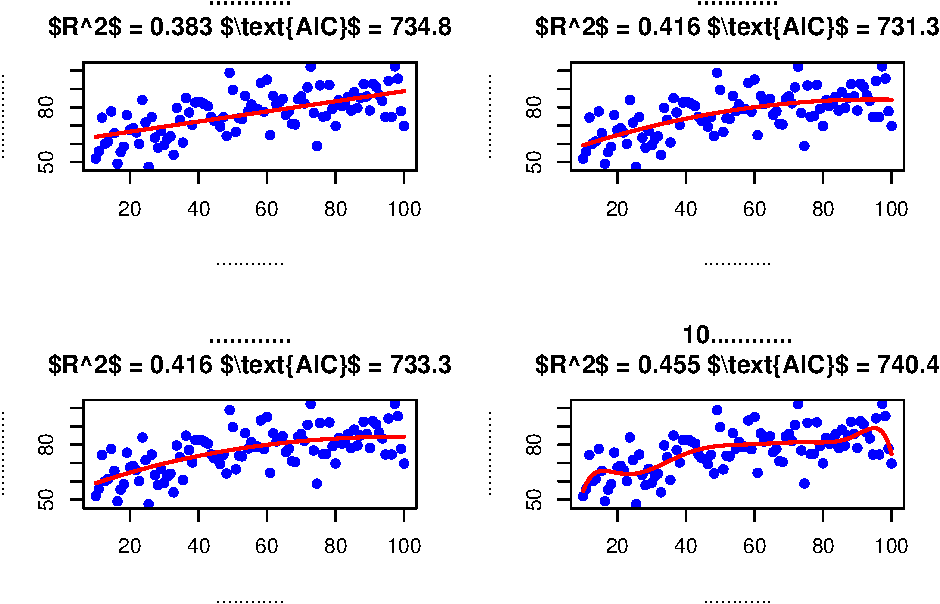
\includegraphics{02-probability_and_distribution_files/figure-latex/unnamed-chunk-3-1} 

}

\caption{大数定律可视化:样本均值随样本量增加收敛于总体均值}\label{fig:unnamed-chunk-3}
\end{figure}

\textbf{频率概率的现实类比}

就像天气预报:气象学家通过分析多年的气象数据,得出某地区在特定季节下雨的概率。

就像质量控制:工厂通过检测大量产品的质量,估计产品合格率。

就像医学研究:通过大规模的临床试验,确定某种药物的有效率。

频率概率让我们从''理想世界''走向''真实世界'',用数据说话,用事实说话。

\hypertarget{ux5b9aux4e49ux4e0eux8ba1ux7b97ux65b9ux6cd5}{%
\subsubsection{定义与计算方法}\label{ux5b9aux4e49ux4e0eux8ba1ux7b97ux65b9ux6cd5}}

频率概率的定义基于长期重复试验的思想。对于一个随机事件A,其频率概率定义为:

\[P(A) = \lim_{n \to \infty} \left( \frac{\text{事件A发生的次数}}{\text{总试验次数}} \right)\]

其中\(n\)表示试验的总次数。在实际应用中,我们通常用有限次试验的频率来近似真实的概率:

\[P(A) \approx \frac{\text{事件A发生的次数}}{\text{总试验次数}}\]

\textbf{频率概率的计算步骤}

\begin{enumerate}
\def\labelenumi{\arabic{enumi}.}
\item
  \textbf{设计观察方案}:确定观察的时间、地点、方法,确保观察的系统性和代表性。
\item
  \textbf{收集数据}:按照设计方案进行重复观察,记录每次试验的结果。
\item
  \textbf{统计频率}:计算事件发生的次数与总观察次数的比值。
\item
  \textbf{评估可靠性}:根据样本大小评估估计的可靠性,样本越大,估计越准确。
\end{enumerate}

\textbf{样本大小的重要性}

在频率概率中,样本大小(观察次数)至关重要。小样本可能受到随机波动的影响,而大样本能够更好地反映真实的概率分布。生态学研究通常需要足够的样本量来获得可靠的估计。

\hypertarget{ux751fux6001ux5b66ux4e2dux7684ux9891ux7387ux6982ux7387ux5e94ux7528}{%
\subsubsection{生态学中的频率概率应用}\label{ux751fux6001ux5b66ux4e2dux7684ux9891ux7387ux6982ux7387ux5e94ux7528}}

频率概率在生态学研究中有着广泛的应用:

\textbf{1. 种群密度估计}

通过样方法调查物种在特定区域的分布频率,可以估计整个种群的密度。例如,在100个样方中发现目标物种的样方比例为30\%,可以推断该物种在整个区域的分布概率约为30\%。

\textbf{2. 行为生态学研究}

通过观察动物行为的频率,可以量化其行为偏好。例如,观察鸟类在不同树种上筑巢的频率,可以了解其对栖息地的选择偏好。

\textbf{3. 物种分布模型}

基于物种在不同环境条件下的出现频率,可以建立物种分布模型,预测物种在未调查区域的分布概率。

\textbf{4. 生态风险评估}

通过分析历史数据中不利事件(如物种灭绝、生态系统崩溃)的发生频率,可以评估未来的生态风险。

\hypertarget{ux9891ux7387ux6982ux7387ux7684ux4f18ux52bfux4e0eux5c40ux9650ux6027}{%
\subsubsection{频率概率的优势与局限性}\label{ux9891ux7387ux6982ux7387ux7684ux4f18ux52bfux4e0eux5c40ux9650ux6027}}

频率概率方法在生态学研究中展现出显著的优势。其\textbf{客观性}确保了概率估计基于实际观察数据而非主观臆断,这为生态学研究提供了坚实的实证基础。通过系统记录生物行为或环境变化,研究者能够获得反映真实世界规律的量化结果。频率概率具有\textbf{可验证性},任何研究者都可以通过重复相同的观察或实验来验证结果的可靠性,这符合科学研究的可重复性原则。在\textbf{实用性}方面,频率概率适用于各种现实世界的概率估计问题,从物种分布调查到种群动态监测,都能提供有效的量化工具。最重要的是,频率概率具有\textbf{渐进精确性},随着样本量的增加,根据大数定律,频率估计会越来越接近真实的概率值,这种自我修正的特性使其成为长期生态监测的理想工具。

然而,频率概率方法也存在明显的局限性。\textbf{需要大量数据}是其最突出的限制,为了获得可靠的估计,通常需要大量的观察数据,这在某些稀有物种或难以观察的行为研究中可能难以实现。\textbf{无法处理一次性事件}是另一个重要局限,对于无法重复的事件(如特定物种的灭绝、罕见自然灾害等),频率概率难以提供有意义的估计。\textbf{历史依赖性}使得基于历史数据的概率估计可能无法准确反映未来的变化,特别是在环境快速变化的背景下,过去的数据可能无法预测未来的趋势。此外,\textbf{样本偏差}问题不容忽视,如果样本选择不具有代表性,或者观察过程中存在系统性偏差,频率估计会产生误导性的结果。这些局限性提醒我们在应用频率概率时需要谨慎考虑其适用条件,并在必要时结合其他概率方法进行综合分析。

频率概率需要大量重复试验,但生态学调查往往样本量有限:

\begin{figure}

{\centering 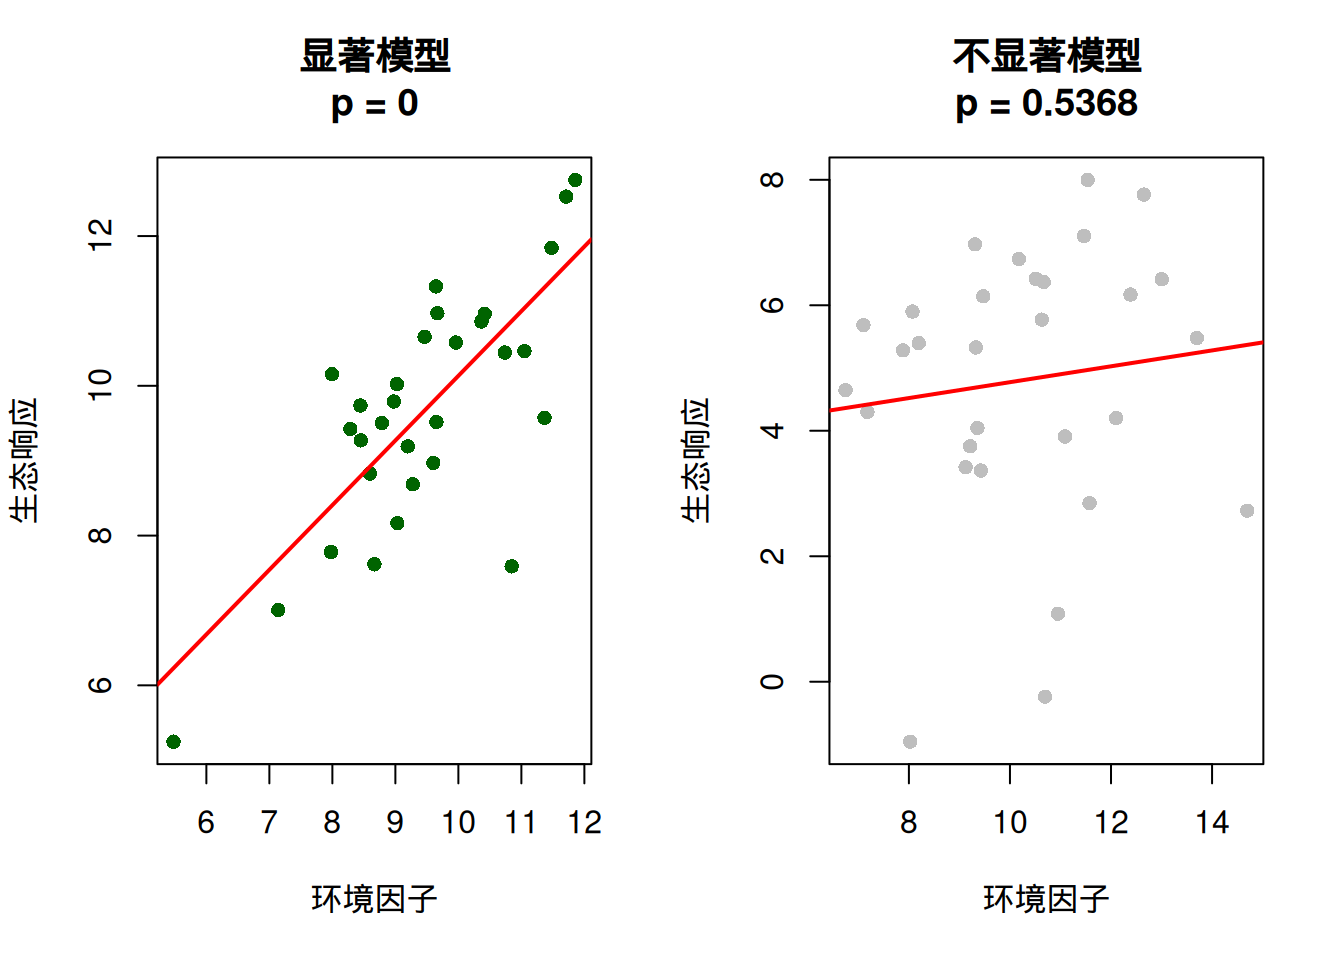
\includegraphics{02-probability_and_distribution_files/figure-latex/unnamed-chunk-4-1} 

}

\caption{样本量对概率估计精度的影响:样本量越大,估计误差越小}\label{fig:unnamed-chunk-4}
\end{figure}

\hypertarget{ux4eceux9891ux7387ux6982ux7387ux5230ux73b0ux4ee3ux7edfux8ba1ux5b66}{%
\subsubsection{从频率概率到现代统计学}\label{ux4eceux9891ux7387ux6982ux7387ux5230ux73b0ux4ee3ux7edfux8ba1ux5b66}}

频率概率为现代统计学的发展奠定了基础。统计推断中的参数估计、假设检验等方法都建立在频率概率的思想之上。20世纪,罗纳德·费希尔、耶日·内曼等统计学家进一步发展了频率统计学的理论体系。

总结来说,频率概率如同生态学家的''望远镜'',让我们能够通过系统的观察来窥见自然界的真实规律。它教会我们''用数据说话''的重要性,培养了我们对实证研究的尊重。当我们面对复杂的生态系统时,频率概率为我们提供了量化不确定性的有力工具,帮助我们基于客观证据做出科学的判断。

\hypertarget{ux52a8ux6001ux7684ux66f4ux65b0ux8d1dux53f6ux65afux6982ux7387}{%
\subsection{动态的更新------贝叶斯概率}\label{ux52a8ux6001ux7684ux66f4ux65b0ux8d1dux53f6ux65afux6982ux7387}}

然而,故事还没结束。一位植物学家告诉我,昨天刚下过雨,三叶草在雨后会特别鲜嫩多汁,营养价值更高。这条新信息(证据)改变了我对你的判断。我不能完全忽略我之前70次观察的结论(先验知识),但我也必须考虑``雨后三叶草更诱人''这个新事实。

\textbf{贝叶斯概率登场了。} 它是一种''信仰''的概率,代表着在\textbf{考虑了新证据之后,我对某个假设(你会选择三叶草)的置信度}。\textbf{它的思维是动态更新的:} 我原来的信念(\(P(\text{选择三叶草}) = 0.07\))是\textbf{先验概率}。得到''昨天下过雨''这个\textbf{证据}后,我利用一个公式(贝叶斯定理)将先验概率和证据结合起来,得到一个更新后的\textbf{后验概率}。这个后验概率可能变成 \(P(\text{选择三叶草} \mid \text{昨天下过雨}) = 0.25\)。这意味着,在''雨后''这个条件下,我认为你选择三叶草的概率从7\%显著提升到了25\%。贝叶斯概率让我们的认知能够随着新证据的出现而不断进化,更像是一种科学的学习过程。

\hypertarget{ux6838ux5fc3ux601dux60f3ux4e3bux89c2ux4fe1ux5ff5ux4e0eux8bc1ux636eux66f4ux65b0}{%
\subsubsection{核心思想:主观信念与证据更新}\label{ux6838ux5fc3ux601dux60f3ux4e3bux89c2ux4fe1ux5ff5ux4e0eux8bc1ux636eux66f4ux65b0}}

贝叶斯概率(也称为主观概率)的核心思想源于认识论哲学------概率是对不确定性的主观度量。与频率概率的''客观''统计不同,贝叶斯概率是''主观''的,它反映了在给定证据条件下对某个假设的置信程度。

\textbf{贝叶斯定理的数学基础}

贝叶斯定理是贝叶斯概率的理论核心。要深入理解贝叶斯定理,我们需要先了解两个关键概念:条件概率和事件独立性。

\hypertarget{ux6761ux4ef6ux6982ux7387ux4e8bux4ef6ux4e4bux95f4ux7684ux4f9dux8d56ux5173ux7cfb}{%
\subsubsection{条件概率:事件之间的依赖关系}\label{ux6761ux4ef6ux6982ux7387ux4e8bux4ef6ux4e4bux95f4ux7684ux4f9dux8d56ux5173ux7cfb}}

\textbf{条件概率} \(P(A|B)\) 表示在事件B已经发生的条件下,事件A发生的概率。这是贝叶斯定理的核心概念。

\textbf{定义}:如果 \(P(B) > 0\),则
\[P(A|B) = \frac{P(A \cap B)}{P(B)}\]

\textbf{生态学示例}:
- \(P(\text{选择三叶草})\) 是无条件概率
- \(P(\text{选择三叶草} \mid \text{昨天下过雨})\) 是条件概率

\hypertarget{ux4e8bux4ef6ux72ecux7acbux6027ux76f8ux4e92ux4e0dux5f71ux54cdux7684ux5173ux7cfb}{%
\subsubsection{事件独立性:相互不影响的关系}\label{ux4e8bux4ef6ux72ecux7acbux6027ux76f8ux4e92ux4e0dux5f71ux54cdux7684ux5173ux7cfb}}

两个事件A和B是\textbf{独立的},如果其中一个事件的发生不影响另一个事件发生的概率。

\textbf{定义}:事件A和B独立当且仅当
\[P(A \cap B) = P(A) \times P(B)\]
等价地,当 \(P(B) > 0\) 且A和B独立时,\(P(A|B) = P(A)\)

\textbf{生态学示例}:
- 如果蚱蜢每天的选择相互独立,那么昨天的选择不影响今天的选择
- 但如果雨后三叶草变得更有吸引力,那么''下雨''和''选择三叶草''就不是独立事件

\hypertarget{ux8d1dux53f6ux65afux5b9aux7406ux7684ux6570ux5b66ux57faux7840}{%
\subsubsection{贝叶斯定理的数学基础}\label{ux8d1dux53f6ux65afux5b9aux7406ux7684ux6570ux5b66ux57faux7840}}

理解了条件概率和独立性后,我们来看贝叶斯定理。这个定理提供了一个数学框架,用于在获得新证据时更新我们对某个假设的信念。其基本形式为:

\[P(H|E) = \frac{P(E|H) \times P(H)}{P(E)}\]

其中:
- \(P(H|E)\) 是后验概率(在证据E条件下假设H的概率)
- \(P(H)\) 是先验概率(在获得证据前对假设H的初始信念)
- \(P(E|H)\) 是似然函数(在假设H成立时观察到证据E的概率)
- \(P(E)\) 是证据的边际概率

\hypertarget{ux5168ux6982ux7387ux516cux5f0fux8ba1ux7b97ux8bc1ux636eux7684ux8fb9ux9645ux6982ux7387}{%
\subsubsection{全概率公式:计算证据的边际概率}\label{ux5168ux6982ux7387ux516cux5f0fux8ba1ux7b97ux8bc1ux636eux7684ux8fb9ux9645ux6982ux7387}}

在贝叶斯定理中,分母\(P(E)\)(证据的边际概率)通常需要通过\textbf{全概率公式}来计算。全概率公式将一个复杂事件的概率分解为多个互斥且完备的情况的概率之和。

\textbf{全概率公式}:如果事件\(B_1, B_2, \ldots, B_n\)构成一个完备事件组(即它们互斥且并集为样本空间),且\(P(B_i) > 0\),则对任意事件A有:
\[P(A) = \sum_{i=1}^{n} P(A|B_i) \times P(B_i)\]

\textbf{生态学示例}:
假设我们想知道''蚱蜢选择营养价值高的植物''的概率\(P(\text{高营养})\)。我们可以将其分解为:
\[P(\text{高营养}) = P(\text{高营养}|\text{晴天}) \times P(\text{晴天}) + P(\text{高营养}|\text{雨天}) \times P(\text{雨天})\]

\begin{figure}

{\centering 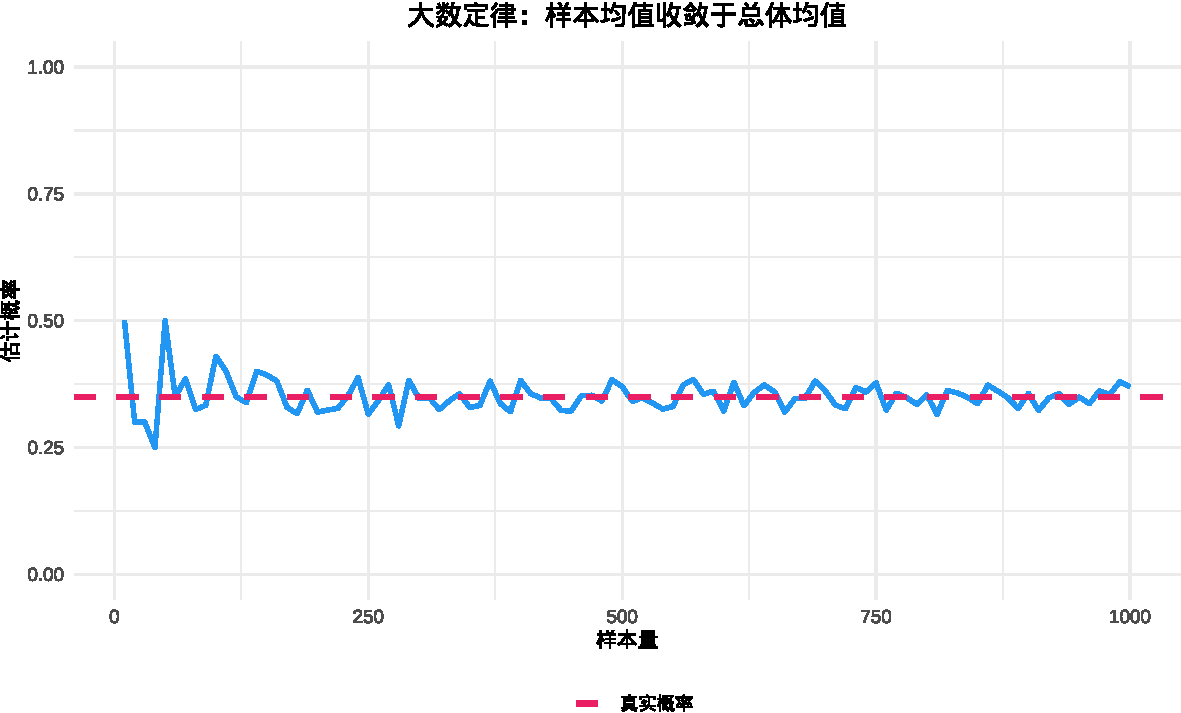
\includegraphics{02-probability_and_distribution_files/figure-latex/unnamed-chunk-5-1} 

}

\caption{全概率公式应用:各情景对总体灭绝概率的贡献分解}\label{fig:unnamed-chunk-5}
\end{figure}

\textbf{在贝叶斯定理中的应用}:
在贝叶斯定理中,\(P(E)\)可以通过全概率公式计算:
\[P(E) = P(E|H) \times P(H) + P(E|\neg H) \times P(\neg H)\]
其中符号\(\neg H\)表示''假设H不成立'',即事件H的补集。

这就得到了贝叶斯定理的完整形式:
\[P(H|E) = \frac{P(E|H) \times P(H)}{P(E|H) \times P(H) + P(E|\neg H) \times P(\neg H)}\]

\textbf{贝叶斯概率的哲学基础}

贝叶斯概率体现了''学习''的本质。我们不是从零开始认识世界,而是基于已有的知识(先验),结合新的观察(证据),不断更新我们的认知(后验)。这种思维方式更接近人类实际的认知过程。

\textbf{贝叶斯概率的现实类比}

就像医学诊断:医生基于患者的症状(证据)更新对疾病的判断(假设)。

就像法庭审判:陪审团基于证据不断更新对被告有罪或无罪的信念。

就像天气预报:气象学家基于新的气象数据更新对天气变化的预测。

贝叶斯概率让我们从''静态世界''走向''动态世界'',用不断更新的信念来应对变化的环境。

\hypertarget{ux5b9aux4e49ux4e0eux8ba1ux7b97ux65b9ux6cd5-1}{%
\subsubsection{定义与计算方法}\label{ux5b9aux4e49ux4e0eux8ba1ux7b97ux65b9ux6cd5-1}}

贝叶斯概率的核心是贝叶斯定理,它提供了一个系统的方法来更新概率估计。通过全概率公式,我们得到了贝叶斯定理的完整形式,它考虑了所有可能的情况,确保概率的归一化。

\textbf{贝叶斯更新的步骤}

\begin{enumerate}
\def\labelenumi{\arabic{enumi}.}
\item
  \textbf{确定先验概率}:基于已有知识或经验,确定对假设的初始信念\(P(H)\)。
\item
  \textbf{计算似然函数}:评估在假设成立时观察到证据的概率\(P(E|H)\)。
\item
  \textbf{计算证据概率}:计算观察到证据的总体概率\(P(E)\)。
\item
  \textbf{计算后验概率}:使用贝叶斯定理更新信念,得到\(P(H|E)\)。
\end{enumerate}

\textbf{先验概率的选择}

在贝叶斯分析中,先验概率的选择具有关键重要性。常用的先验类型包括无信息先验、共轭先验和经验先验。无信息先验适用于缺乏先验知识的情况,为分析提供一个相对中立的起点。共轭先验在数学上能够方便地计算后验分布,简化了贝叶斯更新的计算过程。经验先验则基于历史数据或专家意见,能够将领域知识有机地融入统计模型中。

\textbf{贝叶斯定理基础演示}

\begin{Shaded}
\begin{Highlighting}[]
\CommentTok{\# 贝叶斯定理基础演示:以疾病检测为例展示贝叶斯定理的应用}
\FunctionTok{set.seed}\NormalTok{(}\DecValTok{1111}\NormalTok{)  }\CommentTok{\# 设置随机种子确保结果可重现}

\CommentTok{\# 定义先验概率:基于流行病学知识的初始信念}
\NormalTok{prior\_prob }\OtherTok{\textless{}{-}} \FloatTok{0.05}  \CommentTok{\# 疾病在种群中的患病率(5\%)}

\CommentTok{\# 定义检测准确性参数}
\NormalTok{sensitivity }\OtherTok{\textless{}{-}} \FloatTok{0.95}  \CommentTok{\# 真阳性率:患者被正确检测为阳性的概率}
\NormalTok{specificity }\OtherTok{\textless{}{-}} \FloatTok{0.90}  \CommentTok{\# 真阴性率:健康者被正确检测为阴性的概率}

\CommentTok{\# 计算边际概率 P(阳性):检测结果为阳性的总体概率}
\CommentTok{\# 使用全概率公式:P(阳性) = P(阳性|患病)P(患病) + P(阳性|健康)P(健康)}
\NormalTok{marginal\_positive }\OtherTok{\textless{}{-}}\NormalTok{ prior\_prob }\SpecialCharTok{*}\NormalTok{ sensitivity }\SpecialCharTok{+}
\NormalTok{  (}\DecValTok{1} \SpecialCharTok{{-}}\NormalTok{ prior\_prob) }\SpecialCharTok{*}\NormalTok{ (}\DecValTok{1} \SpecialCharTok{{-}}\NormalTok{ specificity)}

\CommentTok{\# 使用贝叶斯定理计算后验概率 P(患病|阳性)}
\CommentTok{\# 公式:P(患病|阳性) = [P(阳性|患病) × P(患病)] / P(阳性)}
\NormalTok{posterior\_prob }\OtherTok{\textless{}{-}}\NormalTok{ (sensitivity }\SpecialCharTok{*}\NormalTok{ prior\_prob) }\SpecialCharTok{/}\NormalTok{ marginal\_positive}

\CommentTok{\# 输出贝叶斯分析结果}
\FunctionTok{cat}\NormalTok{(}\StringTok{"贝叶斯定理基础演示(疾病检测):}\SpecialCharTok{\textbackslash{}n}\StringTok{"}\NormalTok{,}
  \StringTok{"先验概率 P(患病):"}\NormalTok{, prior\_prob, }\StringTok{"}\SpecialCharTok{\textbackslash{}n}\StringTok{"}\NormalTok{,}
  \StringTok{"检测灵敏度 P(阳性|患病):"}\NormalTok{, sensitivity, }\StringTok{"}\SpecialCharTok{\textbackslash{}n}\StringTok{"}\NormalTok{,}
  \StringTok{"检测特异度 P(阴性|健康):"}\NormalTok{, specificity, }\StringTok{"}\SpecialCharTok{\textbackslash{}n}\StringTok{"}\NormalTok{,}
  \StringTok{"边际概率 P(阳性):"}\NormalTok{, }\FunctionTok{round}\NormalTok{(marginal\_positive, }\DecValTok{4}\NormalTok{), }\StringTok{"}\SpecialCharTok{\textbackslash{}n}\StringTok{"}\NormalTok{,}
  \StringTok{"后验概率 P(患病|阳性):"}\NormalTok{, }\FunctionTok{round}\NormalTok{(posterior\_prob, }\DecValTok{4}\NormalTok{), }\StringTok{"}\SpecialCharTok{\textbackslash{}n}\StringTok{"}\NormalTok{)}
\end{Highlighting}
\end{Shaded}

\begin{verbatim}
## 贝叶斯定理基础演示(疾病检测):
##  先验概率 P(患病): 0.05 
##  检测灵敏度 P(阳性|患病): 0.95 
##  检测特异度 P(阴性|健康): 0.9 
##  边际概率 P(阳性): 0.1425 
##  后验概率 P(患病|阳性): 0.3333
\end{verbatim}

\hypertarget{ux751fux6001ux5b66ux4e2dux7684ux8d1dux53f6ux65afux6982ux7387ux5e94ux7528}{%
\subsubsection{生态学中的贝叶斯概率应用}\label{ux751fux6001ux5b66ux4e2dux7684ux8d1dux53f6ux65afux6982ux7387ux5e94ux7528}}

贝叶斯概率在现代生态学研究中越来越重要:

\textbf{1. 物种分布模型}

结合专家知识和观测数据,建立更准确的物种分布预测模型。先验可以反映物种的生态习性,后验则结合了实际的分布数据。

贝叶斯方法在物种分布建模中具有独特优势,能够结合专家知识和观测数据:

\begin{Shaded}
\begin{Highlighting}[]
\CommentTok{\# 贝叶斯物种分布模型}
\CommentTok{\# 演示如何结合专家知识和观测数据更新物种栖息地偏好}

\CommentTok{\# 设置随机种子确保结果可重现}
\FunctionTok{set.seed}\NormalTok{(}\DecValTok{1414}\NormalTok{)}

\CommentTok{\# 定义先验信息:基于专家经验的初始信念}
\CommentTok{\# 专家认为物种偏好森林(60\%)、草地(30\%)、湿地(10\%)}
\NormalTok{expert\_prior }\OtherTok{\textless{}{-}} \FunctionTok{c}\NormalTok{(}\FloatTok{0.6}\NormalTok{, }\FloatTok{0.3}\NormalTok{, }\FloatTok{0.1}\NormalTok{)}
\NormalTok{habitat\_types }\OtherTok{\textless{}{-}} \FunctionTok{c}\NormalTok{(}\StringTok{"森林"}\NormalTok{, }\StringTok{"草地"}\NormalTok{, }\StringTok{"湿地"}\NormalTok{)}

\CommentTok{\# 定义观测数据:在不同栖息地中实际发现物种的次数}
\NormalTok{observations }\OtherTok{\textless{}{-}} \FunctionTok{c}\NormalTok{(}\DecValTok{45}\NormalTok{, }\DecValTok{20}\NormalTok{, }\DecValTok{5}\NormalTok{)  }\CommentTok{\# 森林45次,草地20次,湿地5次}
\NormalTok{total\_observations }\OtherTok{\textless{}{-}} \FunctionTok{sum}\NormalTok{(observations)  }\CommentTok{\# 总观测次数}

\CommentTok{\# 计算似然函数:基于观测数据的条件概率}
\CommentTok{\# 似然 = 各栖息地观测次数 / 总观测次数}
\NormalTok{likelihood }\OtherTok{\textless{}{-}}\NormalTok{ observations }\SpecialCharTok{/}\NormalTok{ total\_observations}

\CommentTok{\# 计算证据概率(标准化常数):使用全概率公式}
\CommentTok{\# 证据 = Σ(先验 × 似然)}
\NormalTok{evidence }\OtherTok{\textless{}{-}} \FunctionTok{sum}\NormalTok{(expert\_prior }\SpecialCharTok{*}\NormalTok{ likelihood)}

\CommentTok{\# 贝叶斯更新:计算后验概率}
\CommentTok{\# 后验 = (先验 × 似然) / 证据}
\NormalTok{posterior }\OtherTok{\textless{}{-}}\NormalTok{ (expert\_prior }\SpecialCharTok{*}\NormalTok{ likelihood) }\SpecialCharTok{/}\NormalTok{ evidence}

\CommentTok{\# 创建结果数据框,便于比较分析}
\NormalTok{results }\OtherTok{\textless{}{-}} \FunctionTok{data.frame}\NormalTok{(}
\NormalTok{  栖息地类型 }\OtherTok{=}\NormalTok{ habitat\_types,}
\NormalTok{  专家先验 }\OtherTok{=} \FunctionTok{round}\NormalTok{(expert\_prior, }\DecValTok{3}\NormalTok{),    }\CommentTok{\# 四舍五入到3位小数}
\NormalTok{  观测似然 }\OtherTok{=} \FunctionTok{round}\NormalTok{(likelihood, }\DecValTok{3}\NormalTok{),      }\CommentTok{\# 四舍五入到3位小数}
\NormalTok{  贝叶斯后验 }\OtherTok{=} \FunctionTok{round}\NormalTok{(posterior, }\DecValTok{3}\NormalTok{)      }\CommentTok{\# 四舍五入到3位小数}
\NormalTok{)}

\CommentTok{\# 输出模型结果}
\FunctionTok{cat}\NormalTok{(}\StringTok{"贝叶斯物种分布模型结果:}\SpecialCharTok{\textbackslash{}n}\StringTok{"}\NormalTok{)}
\end{Highlighting}
\end{Shaded}

\begin{verbatim}
## 贝叶斯物种分布模型结果:
\end{verbatim}

\begin{Shaded}
\begin{Highlighting}[]
\FunctionTok{print}\NormalTok{(results)}
\end{Highlighting}
\end{Shaded}

\begin{verbatim}
##   栖息地类型 专家先验 观测似然 贝叶斯后验
## 1       森林      0.6    0.643      0.806
## 2       草地      0.3    0.286      0.179
## 3       湿地      0.1    0.071      0.015
\end{verbatim}

\begin{Shaded}
\begin{Highlighting}[]
\CommentTok{\# 计算信息增益:使用KL散度量化先验到后验的信息变化}
\CommentTok{\# KL散度 = Σ(后验 × log(后验/先验))}
\NormalTok{kl\_divergence }\OtherTok{\textless{}{-}} \FunctionTok{sum}\NormalTok{(posterior }\SpecialCharTok{*} \FunctionTok{log}\NormalTok{(posterior }\SpecialCharTok{/}\NormalTok{ expert\_prior))}
\FunctionTok{cat}\NormalTok{(}\StringTok{"KL散度(信息增益):"}\NormalTok{, }\FunctionTok{round}\NormalTok{(kl\_divergence, }\DecValTok{4}\NormalTok{), }\StringTok{"}\SpecialCharTok{\textbackslash{}n}\StringTok{"}\NormalTok{)}
\end{Highlighting}
\end{Shaded}

\begin{verbatim}
## KL散度(信息增益): 0.1171
\end{verbatim}

\begin{Shaded}
\begin{Highlighting}[]
\CommentTok{\# 计算贝叶斯因子:比较森林偏好假设的证据强度}
\CommentTok{\# 贝叶斯因子 = (后验优势比) / (先验优势比)}
\NormalTok{bayes\_factor }\OtherTok{\textless{}{-}}\NormalTok{ (posterior[}\DecValTok{1}\NormalTok{] }\SpecialCharTok{/}\NormalTok{ (}\DecValTok{1} \SpecialCharTok{{-}}\NormalTok{ posterior[}\DecValTok{1}\NormalTok{])) }\SpecialCharTok{/}
\NormalTok{  (expert\_prior[}\DecValTok{1}\NormalTok{] }\SpecialCharTok{/}\NormalTok{ (}\DecValTok{1} \SpecialCharTok{{-}}\NormalTok{ expert\_prior[}\DecValTok{1}\NormalTok{]))}
\FunctionTok{cat}\NormalTok{(}\StringTok{"贝叶斯因子(森林偏好):"}\NormalTok{, }\FunctionTok{round}\NormalTok{(bayes\_factor, }\DecValTok{2}\NormalTok{), }\StringTok{"}\SpecialCharTok{\textbackslash{}n}\StringTok{"}\NormalTok{)}
\end{Highlighting}
\end{Shaded}

\begin{verbatim}
## 贝叶斯因子(森林偏好): 2.77
\end{verbatim}

\begin{Shaded}
\begin{Highlighting}[]
\CommentTok{\# 根据贝叶斯因子大小判断证据强度}
\ControlFlowTok{if}\NormalTok{ (bayes\_factor }\SpecialCharTok{\textgreater{}} \DecValTok{3}\NormalTok{) \{}
  \FunctionTok{cat}\NormalTok{(}\StringTok{"强烈支持物种偏好森林的假设}\SpecialCharTok{\textbackslash{}n}\StringTok{"}\NormalTok{)}
\NormalTok{\} }\ControlFlowTok{else} \ControlFlowTok{if}\NormalTok{ (bayes\_factor }\SpecialCharTok{\textgreater{}} \DecValTok{1}\NormalTok{) \{}
  \FunctionTok{cat}\NormalTok{(}\StringTok{"微弱支持物种偏好森林的假设}\SpecialCharTok{\textbackslash{}n}\StringTok{"}\NormalTok{)}
\NormalTok{\} }\ControlFlowTok{else}\NormalTok{ \{}
  \FunctionTok{cat}\NormalTok{(}\StringTok{"证据不支持物种偏好森林的假设}\SpecialCharTok{\textbackslash{}n}\StringTok{"}\NormalTok{)}
\NormalTok{\}}
\end{Highlighting}
\end{Shaded}

\begin{verbatim}
## 微弱支持物种偏好森林的假设
\end{verbatim}

\textbf{2. 种群动态预测}

基于历史种群数据和环境变化信息,预测未来种群数量的变化趋势。贝叶斯方法能够处理参数的不确定性。

\textbf{3. 保护优先级评估}

结合多种证据(如栖息地质量、种群趋势、威胁因素)来评估物种的保护优先级。

\begin{figure}

{\centering 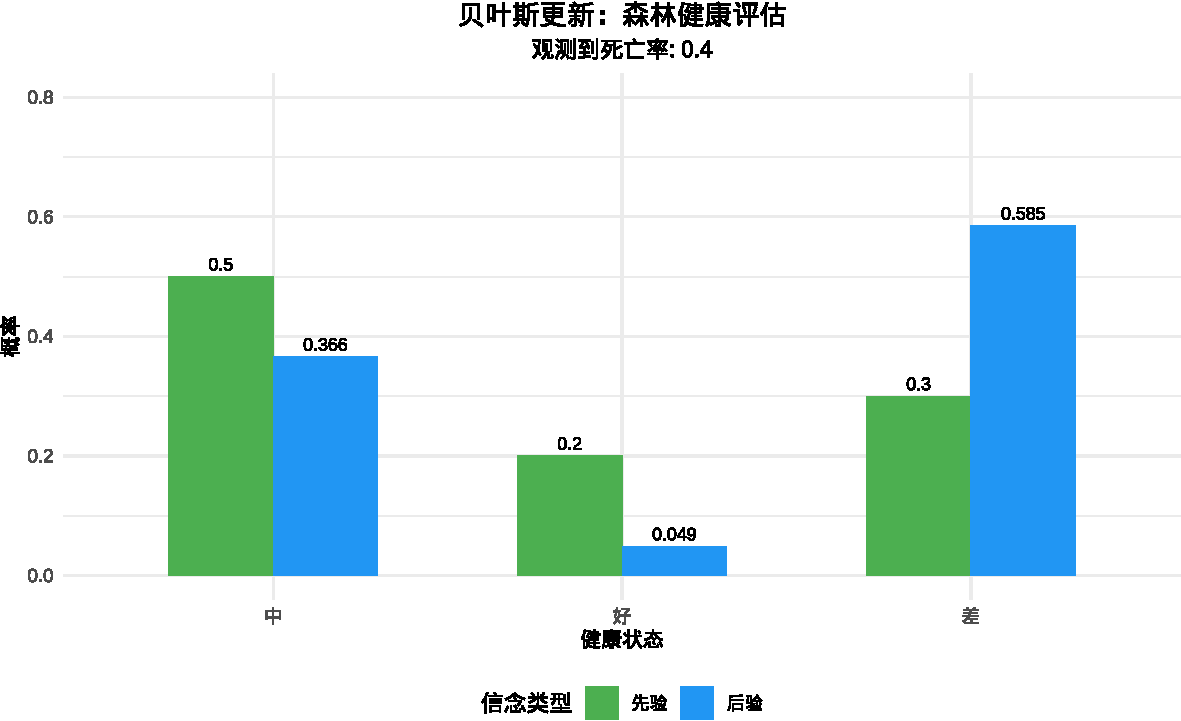
\includegraphics{02-probability_and_distribution_files/figure-latex/unnamed-chunk-8-1} 

}

\caption{贝叶斯更新过程:森林健康评估中先验信念到后验信念的转变}\label{fig:unnamed-chunk-8}
\end{figure}

\textbf{4. 生态风险评估}

在数据有限的情况下,结合专家判断和有限观测来评估生态风险。

\begin{figure}

{\centering \includegraphics{02-probability_and_distribution_files/figure-latex/unnamed-chunk-9-1} 

}

\caption{贝叶斯风险评估与决策分析:基于新证据的风险概率更新和成本效益决策}\label{fig:unnamed-chunk-9}
\end{figure}

\textbf{5. 模型选择与平均}

使用贝叶斯模型平均方法,综合考虑多个竞争模型的预测结果。

\begin{verbatim}
## 贝叶斯模型比较结果:
\end{verbatim}

\begin{verbatim}
##       模型     模型证据 贝叶斯因子
## 1 线性模型 7.411531e-52       1.00
## 2 季节模型 1.036188e-47   13980.76
\end{verbatim}

\begin{figure}

{\centering 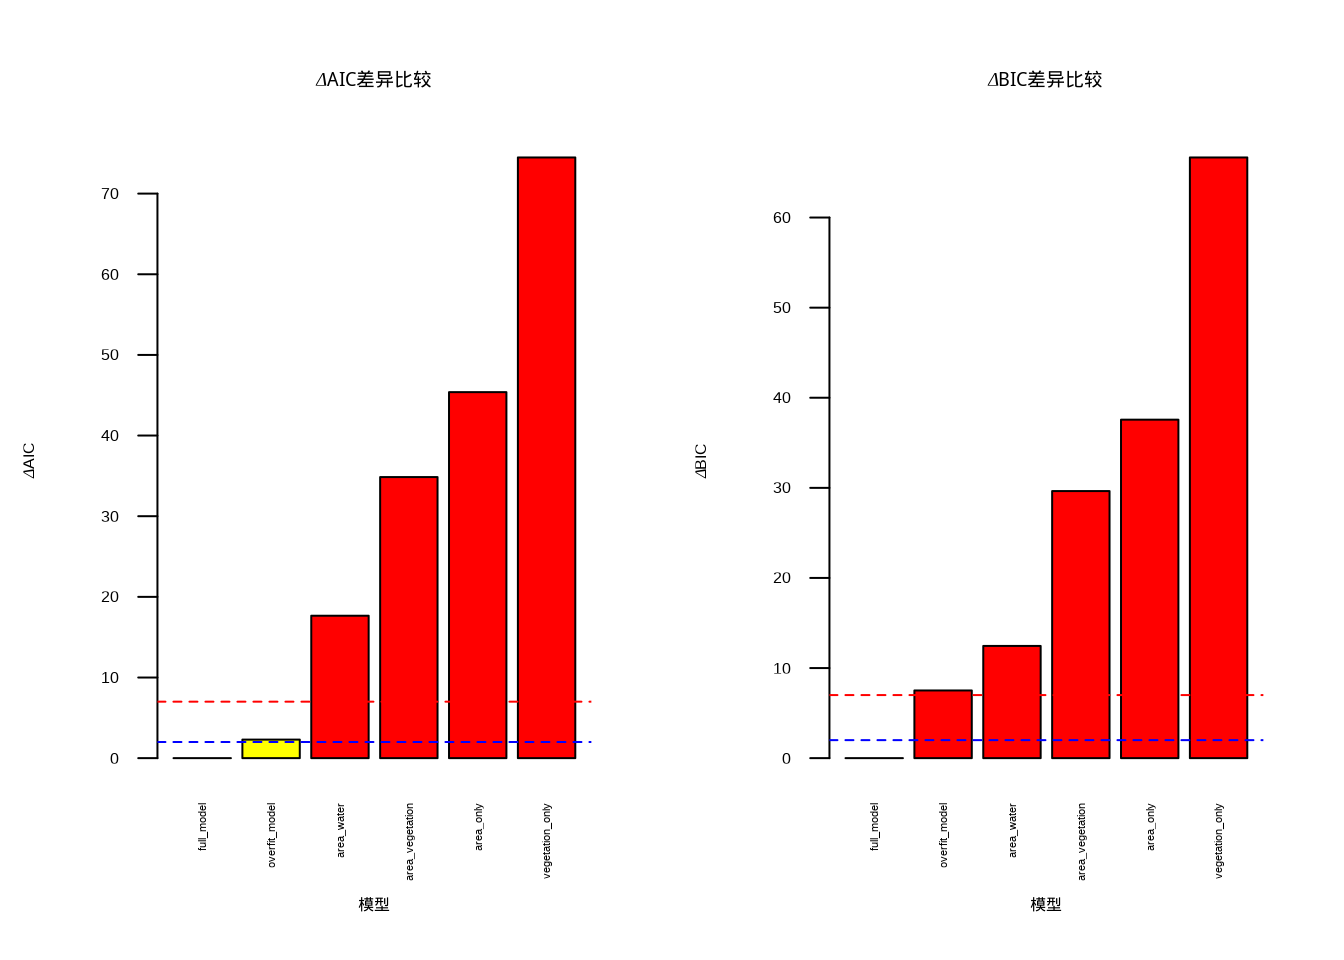
\includegraphics{02-probability_and_distribution_files/figure-latex/unnamed-chunk-10-1} 

}

\caption{贝叶斯模型比较:线性模型与季节模型对种群增长模式的拟合效果对比}\label{fig:unnamed-chunk-10}
\end{figure}

敏感性分析与稳健性检验

\begin{Shaded}
\begin{Highlighting}[]
\CommentTok{\# 贝叶斯敏感性分析函数定义}
\NormalTok{sensitivity\_analysis }\OtherTok{\textless{}{-}} \ControlFlowTok{function}\NormalTok{(prior\_strength) \{}
  \CommentTok{\# 不同先验强度下的后验分析}
  \FunctionTok{set.seed}\NormalTok{(}\DecValTok{1717}\NormalTok{)}

  \CommentTok{\# 生成生态数据}
\NormalTok{  true\_effect }\OtherTok{\textless{}{-}} \FloatTok{0.8}
\NormalTok{  observed\_data }\OtherTok{\textless{}{-}} \FunctionTok{rnorm}\NormalTok{(}\DecValTok{30}\NormalTok{, true\_effect, }\FloatTok{0.5}\NormalTok{)}

  \CommentTok{\# 不同先验强度}
\NormalTok{  prior\_sd }\OtherTok{\textless{}{-}} \DecValTok{10} \SpecialCharTok{/}\NormalTok{ prior\_strength }\CommentTok{\# 先验标准差随强度变化}

  \CommentTok{\# 简单贝叶斯更新}
\NormalTok{  prior\_mean }\OtherTok{\textless{}{-}} \DecValTok{0}
\NormalTok{  sample\_mean }\OtherTok{\textless{}{-}} \FunctionTok{mean}\NormalTok{(observed\_data)}
\NormalTok{  sample\_sd }\OtherTok{\textless{}{-}} \FunctionTok{sd}\NormalTok{(observed\_data) }\SpecialCharTok{/} \FunctionTok{sqrt}\NormalTok{(}\FunctionTok{length}\NormalTok{(observed\_data))}

  \CommentTok{\# 后验计算(正态{-}正态共轭)}
\NormalTok{  posterior\_precision }\OtherTok{\textless{}{-}} \DecValTok{1} \SpecialCharTok{/}\NormalTok{ prior\_sd}\SpecialCharTok{\^{}}\DecValTok{2} \SpecialCharTok{+} \DecValTok{1} \SpecialCharTok{/}\NormalTok{ sample\_sd}\SpecialCharTok{\^{}}\DecValTok{2}
\NormalTok{  posterior\_mean }\OtherTok{\textless{}{-}}\NormalTok{ (prior\_mean }\SpecialCharTok{/}\NormalTok{ prior\_sd}\SpecialCharTok{\^{}}\DecValTok{2} \SpecialCharTok{+}
\NormalTok{                     sample\_mean }\SpecialCharTok{/}\NormalTok{ sample\_sd}\SpecialCharTok{\^{}}\DecValTok{2}\NormalTok{) }\SpecialCharTok{/}\NormalTok{ posterior\_precision}
\NormalTok{  posterior\_sd }\OtherTok{\textless{}{-}} \FunctionTok{sqrt}\NormalTok{(}\DecValTok{1} \SpecialCharTok{/}\NormalTok{ posterior\_precision)}

  \FunctionTok{return}\NormalTok{(}\FunctionTok{c}\NormalTok{(posterior\_mean, posterior\_sd))}
\NormalTok{\}}
\end{Highlighting}
\end{Shaded}

\begin{Shaded}
\begin{Highlighting}[]
\CommentTok{\# 敏感性分析:测试不同先验强度}
\NormalTok{prior\_strengths }\OtherTok{\textless{}{-}} \FunctionTok{c}\NormalTok{(}\FloatTok{0.1}\NormalTok{, }\FloatTok{0.5}\NormalTok{, }\DecValTok{1}\NormalTok{, }\DecValTok{2}\NormalTok{, }\DecValTok{5}\NormalTok{, }\DecValTok{10}\NormalTok{)}
\NormalTok{sensitivity\_results }\OtherTok{\textless{}{-}} \FunctionTok{t}\NormalTok{(}\FunctionTok{sapply}\NormalTok{(prior\_strengths, sensitivity\_analysis))}

\NormalTok{sensitivity\_df }\OtherTok{\textless{}{-}} \FunctionTok{data.frame}\NormalTok{(}
\NormalTok{  先验强度 }\OtherTok{=}\NormalTok{ prior\_strengths,}
\NormalTok{  后验均值 }\OtherTok{=} \FunctionTok{round}\NormalTok{(sensitivity\_results[, }\DecValTok{1}\NormalTok{], }\DecValTok{3}\NormalTok{),}
\NormalTok{  后验标准差 }\OtherTok{=} \FunctionTok{round}\NormalTok{(sensitivity\_results[, }\DecValTok{2}\NormalTok{], }\DecValTok{3}\NormalTok{)}
\NormalTok{)}

\FunctionTok{cat}\NormalTok{(}\StringTok{"贝叶斯敏感性分析结果:}\SpecialCharTok{\textbackslash{}n}\StringTok{"}\NormalTok{)}
\end{Highlighting}
\end{Shaded}

\begin{verbatim}
## 贝叶斯敏感性分析结果:
\end{verbatim}

\begin{Shaded}
\begin{Highlighting}[]
\FunctionTok{print}\NormalTok{(sensitivity\_df)}
\end{Highlighting}
\end{Shaded}

\begin{verbatim}
##   先验强度 后验均值 后验标准差
## 1      0.1    0.708      0.097
## 2      0.5    0.708      0.097
## 3      1.0    0.708      0.097
## 4      2.0    0.708      0.097
## 5      5.0    0.706      0.097
## 6     10.0    0.702      0.096
\end{verbatim}

\begin{Shaded}
\begin{Highlighting}[]
\CommentTok{\# 稳健性检验函数定义}
\NormalTok{robustness\_check }\OtherTok{\textless{}{-}} \ControlFlowTok{function}\NormalTok{(data\_contamination) \{}
  \CommentTok{\# 检验数据污染对结果的影响}
  \FunctionTok{set.seed}\NormalTok{(}\DecValTok{1818}\NormalTok{)}

  \CommentTok{\# 生成清洁数据}
\NormalTok{  clean\_data }\OtherTok{\textless{}{-}} \FunctionTok{rnorm}\NormalTok{(}\DecValTok{25}\NormalTok{, }\FloatTok{0.5}\NormalTok{, }\FloatTok{0.3}\NormalTok{)}

  \CommentTok{\# 添加污染数据}
\NormalTok{  n\_contaminated }\OtherTok{\textless{}{-}} \FunctionTok{round}\NormalTok{(}\FunctionTok{length}\NormalTok{(clean\_data) }\SpecialCharTok{*}\NormalTok{ data\_contamination)}
  \ControlFlowTok{if}\NormalTok{ (n\_contaminated }\SpecialCharTok{\textgreater{}} \DecValTok{0}\NormalTok{) \{}
\NormalTok{    contaminated\_data }\OtherTok{\textless{}{-}} \FunctionTok{rnorm}\NormalTok{(n\_contaminated, }\FloatTok{2.0}\NormalTok{, }\FloatTok{0.5}\NormalTok{) }\CommentTok{\# 异常值}
\NormalTok{    all\_data }\OtherTok{\textless{}{-}} \FunctionTok{c}\NormalTok{(clean\_data, contaminated\_data)}
\NormalTok{  \} }\ControlFlowTok{else}\NormalTok{ \{}
\NormalTok{    all\_data }\OtherTok{\textless{}{-}}\NormalTok{ clean\_data}
\NormalTok{  \}}

  \CommentTok{\# 贝叶斯分析}
\NormalTok{  prior\_mean }\OtherTok{\textless{}{-}} \DecValTok{0}
\NormalTok{  prior\_sd }\OtherTok{\textless{}{-}} \DecValTok{1}

\NormalTok{  sample\_mean }\OtherTok{\textless{}{-}} \FunctionTok{mean}\NormalTok{(all\_data)}
\NormalTok{  sample\_sd }\OtherTok{\textless{}{-}} \FunctionTok{sd}\NormalTok{(all\_data) }\SpecialCharTok{/} \FunctionTok{sqrt}\NormalTok{(}\FunctionTok{length}\NormalTok{(all\_data))}

\NormalTok{  posterior\_precision }\OtherTok{\textless{}{-}} \DecValTok{1} \SpecialCharTok{/}\NormalTok{ prior\_sd}\SpecialCharTok{\^{}}\DecValTok{2} \SpecialCharTok{+} \DecValTok{1} \SpecialCharTok{/}\NormalTok{ sample\_sd}\SpecialCharTok{\^{}}\DecValTok{2}
\NormalTok{  posterior\_mean }\OtherTok{\textless{}{-}}\NormalTok{ (prior\_mean }\SpecialCharTok{/}\NormalTok{ prior\_sd}\SpecialCharTok{\^{}}\DecValTok{2} \SpecialCharTok{+}
\NormalTok{                     sample\_mean }\SpecialCharTok{/}\NormalTok{ sample\_sd}\SpecialCharTok{\^{}}\DecValTok{2}\NormalTok{) }\SpecialCharTok{/}\NormalTok{ posterior\_precision}

  \FunctionTok{return}\NormalTok{(posterior\_mean)}
\NormalTok{\}}
\end{Highlighting}
\end{Shaded}

\begin{Shaded}
\begin{Highlighting}[]
\CommentTok{\# 稳健性检验:测试不同污染水平}
\NormalTok{contamination\_levels }\OtherTok{\textless{}{-}} \FunctionTok{c}\NormalTok{(}\DecValTok{0}\NormalTok{, }\FloatTok{0.05}\NormalTok{, }\FloatTok{0.1}\NormalTok{, }\FloatTok{0.2}\NormalTok{, }\FloatTok{0.3}\NormalTok{)}
\NormalTok{robustness\_results }\OtherTok{\textless{}{-}} \FunctionTok{sapply}\NormalTok{(contamination\_levels, robustness\_check)}

\NormalTok{robustness\_df }\OtherTok{\textless{}{-}} \FunctionTok{data.frame}\NormalTok{(}
\NormalTok{  污染比例 }\OtherTok{=}\NormalTok{ contamination\_levels,}
\NormalTok{  后验均值 }\OtherTok{=} \FunctionTok{round}\NormalTok{(robustness\_results, }\DecValTok{3}\NormalTok{)}
\NormalTok{)}

\FunctionTok{cat}\NormalTok{(}\StringTok{"}\SpecialCharTok{\textbackslash{}n}\StringTok{贝叶斯稳健性检验结果:}\SpecialCharTok{\textbackslash{}n}\StringTok{"}\NormalTok{)}
\end{Highlighting}
\end{Shaded}

\begin{verbatim}
## 
## 贝叶斯稳健性检验结果:
\end{verbatim}

\begin{Shaded}
\begin{Highlighting}[]
\FunctionTok{print}\NormalTok{(robustness\_df)}
\end{Highlighting}
\end{Shaded}

\begin{verbatim}
##   污染比例 后验均值
## 1     0.00    0.539
## 2     0.05    0.604
## 3     0.10    0.683
## 4     0.20    0.804
## 5     0.30    0.888
\end{verbatim}

\hypertarget{ux8d1dux53f6ux65afux6982ux7387ux7684ux4f18ux52bfux4e0eux5c40ux9650ux6027}{%
\subsubsection{贝叶斯概率的优势与局限性}\label{ux8d1dux53f6ux65afux6982ux7387ux7684ux4f18ux52bfux4e0eux5c40ux9650ux6027}}

贝叶斯概率方法在现代生态学研究中展现出独特的优势。其\textbf{灵活性}体现在能够有机地结合先验知识和新的观测证据,这种动态更新的特性使其特别适合处理环境变化和物种适应性研究。通过贝叶斯定理,研究者可以将专家经验、历史数据与最新的实地观察相结合,形成更加全面的认知。\textbf{不确定性量化}是贝叶斯方法的另一重要优势,它不仅提供点估计,还能明确表达参数的不确定性范围,这对于生态风险评估和保护决策具有重要意义。在\textbf{小样本适用性}方面,贝叶斯方法在数据有限的情况下仍然能够发挥作用,这对于研究稀有物种或难以大规模观察的生态现象尤为宝贵。\textbf{模型复杂性处理}能力使贝叶斯方法能够应对生态学中常见的多层次、多变量复杂系统,如考虑个体差异、空间异质性和时间动态的生态模型。最重要的是,贝叶斯方法提供\textbf{决策支持},直接输出决策所需的概率信息,如物种灭绝风险、保护措施效果等,为生态管理提供科学依据。

然而,贝叶斯概率方法也存在不容忽视的局限性。\textbf{主观性}是其最受争议的方面,先验概率的选择往往依赖于研究者的主观判断,不同专家可能会给出不同的先验设定。\textbf{计算复杂性}是实际应用中的主要障碍,复杂的贝叶斯模型需要大量的计算资源,特别是使用马尔可夫链蒙特卡洛方法时,计算时间可能相当可观。\textbf{先验敏感性}问题意味着结果可能对先验选择高度敏感,不恰当的先验设定可能导致有偏的结论。\textbf{收敛问题}是MCMC方法特有的挑战,在复杂模型中可能出现收敛困难或收敛到局部最优解的情况。此外,\textbf{解释难度}限制了贝叶斯方法的普及,后验分布的理解和解释需要研究者具备相当的统计背景,这在一定程度上阻碍了其在生态学实践中的广泛应用。这些局限性提示我们在使用贝叶斯方法时需要谨慎处理先验设定,并充分考虑计算可行性和结果解释的清晰性。

\begin{figure}

{\centering \includegraphics{02-probability_and_distribution_files/figure-latex/unnamed-chunk-15-1} 

}

\caption{主观偏见问题:不同群体对同一生态风险评估的差异}\label{fig:unnamed-chunk-15}
\end{figure}

\hypertarget{ux8d1dux53f6ux65afux7edfux8ba1ux7684ux6311ux6218ux53caux89e3ux51b3ux65b9ux6848}{%
\subsubsection{贝叶斯统计的挑战及解决方案}\label{ux8d1dux53f6ux65afux7edfux8ba1ux7684ux6311ux6218ux53caux89e3ux51b3ux65b9ux6848}}

贝叶斯框架在概念上非常优雅,但在计算上有一个巨大的挑战:\textbf{分母 \(P(E)\) 通常极其难以计算。}

\[ P(E) = \int P(E \mid \theta) P(\theta) \, d\theta \]

这个积分在高维空间(即参数\(\theta\)包含多个变量时)往往没有解析解(即无法用公式直接写出结果)。这严重限制了贝叶斯方法的应用,人们只能对那些具有``共轭先验''的特殊模型进行分析(即先验和后验属于同一分布家族,从而可以避开积分计算)。

\textbf{所以,问题的核心变成了:如何有效地从复杂的、高维的后验分布 \(P(\theta \mid E)\) 中获取信息(例如,计算均值、方差、分位数等),而无需知道那个讨厌的分母 \(P(E)\)?}

\textbf{马尔可夫模拟(MCMC)的核心思想}

MCMC是一类算法的总称,它巧妙地解决了上述挑战。它的核心思想是:

\textbf{与其直接计算后验分布,不如我们构造一个马尔可夫链,使其平稳分布恰好就是我们想要的后验分布 \(P(\theta \mid E)\)。然后,我们从这个链中生成大量的样本,用这些样本来近似(模拟)后验分布。}

想象一下,你是一个盲人,想要了解一头大象的形状。这头大象就是贝叶斯统计中的\textbf{后验分布}------我们想要了解但无法直接看到的复杂概率分布。

\textbf{贝叶斯的难题}:大象的形状太复杂了,你无法用数学公式精确描述它(就像无法直接计算分母P(E)一样)。

\textbf{MCMC的解决方案}:你不需要知道大象的精确形状,只需要通过''触摸''来了解它:

\begin{enumerate}
\def\labelenumi{\arabic{enumi}.}
\item
  \textbf{马尔可夫链}:你开始在大象周围随机走动,但遵循一个聪明的规则------每次移动时,你更倾向于走向大象''更胖''的区域(高概率区域),而不是''更瘦''的区域(低概率区域)。
\item
  \textbf{蒙特卡洛抽样}:你边走边触摸大象,记录下每个位置的感受。虽然每次触摸只能了解一小部分,但经过成千上万次触摸后,你就能在心中构建出大象的整体形状。
\item
  \textbf{巧妙之处}:你根本不需要知道大象的确切形状!你只需要比较当前位置和下一个位置哪个''更胖''(通过概率比值),这个比值中讨厌的分母P(E)会自动抵消掉。
\end{enumerate}

\textbf{结果}:经过足够多的''触摸''后,你收集到的位置样本就精确地反映了大象的真实形状。你可以通过这些样本计算大象的平均高度(后验均值)、宽度(后验方差),甚至画出大象的轮廓(后验分布图)。

就像盲人通过系统性的触摸来了解复杂的大象形状一样,MCMC通过系统性的随机游走来探索复杂的生态学后验分布,让我们能够在不知道精确数学解的情况下,仍然能够对生态系统的参数做出可靠的贝叶斯推断。

我们来用正式的语言分解MCMC这个思想:

\begin{enumerate}
\def\labelenumi{\arabic{enumi}.}
\item
  \textbf{蒙特卡洛(Monte Carlo)}: 泛指通过随机抽样来解决问题的方法。基本思想是:如果你想知道一个分布的属性(比如均值),就从该分布中抽取大量样本,然后计算这些样本的均值。\textbf{问题在于}:我们无法直接从复杂的后验分布中抽样。
\item
  \textbf{马尔可夫链(Markov Chain)}: 这是一个具有``无记忆''性质的随机过程,下一个状态只取决于当前状态,而与过去的状态无关。关键点是,在满足一定条件下,马尔可夫链会收敛到一个唯一的\textbf{平稳分布}。这意味着无论链从何处开始,经过足够长的步骤后,它停留在每个状态的概率是固定的。
\item
  \textbf{MCMC的巧妙结合}:
  \textbf{目标}是让后验分布 \(P(\theta \mid E)\) 成为马尔可夫链的平稳分布。\textbf{方法}是设计特定的规则(如Metropolis-Hastings算法或Gibbs抽样),来构建这样一个链。这些规则的伟大之处在于,它们在计算时,\textbf{分母 \(P(E)\) 会被约掉!} 因为规则中只涉及后验分布的\emph{比值}:
  \[ \frac{P(\theta_{\text{新}} \mid E)}{P(\theta_{\text{旧}} \mid E)} = \frac{\frac{P(E \mid \theta_{\text{新}})P(\theta_{\text{新}})}{P(E)}}{\frac{P(E \mid \theta_{\text{旧}})P(\theta_{\text{旧}})}{P(E)}} = \frac{P(E \mid \theta_{\text{新}})P(\theta_{\text{新}})}{P(E \mid \theta_{\text{旧}})P(\theta_{\text{旧}})} \]
  \(P(E)\) 被完美地消去了。所以我们可以在完全不知道 \(P(E)\) 的情况下,判断是否应该从当前参数 \(\theta_{\text{旧}}\) 移动到新参数 \(\theta_{\text{新}}\)。\textbf{过程}是算法从某个初始值开始,然后根据规则随机游走。经过一段''预烧期''后,链会收敛到平稳分布。之后产生的样本,虽然彼此相关(因为是马尔可夫链),但可以看作是来自后验分布 \(P(\theta \mid E)\) 的(近似)样本。
\end{enumerate}

\textbf{两者的关系------完美的共生}

现在我们可以清晰地描述贝叶斯统计与马尔可夫链蒙特卡洛方法之间的关系。

在\textbf{目标与手段的关系}中,贝叶斯统计定义了我们要解决的核心问题------求得后验分布,而MCMC则提供了实现这一目标的计算引擎。没有MCMC的强大计算能力,贝叶斯理论对于许多复杂模型只能停留在''纸上谈兵''的阶段,无法在实际应用中发挥作用。

\textbf{计算上的突破}体现在MCMC的出现,特别是在1990年代以后,这成为贝叶斯统计复兴和广泛应用的根本原因。MCMC使得分析者能够自由地构建复杂的、非共轭的、高维的模型,而无需担心无法计算的积分问题。几乎所有现代的贝叶斯软件,如Stan、PyMC和JAGS,其核心计算引擎都基于MCMC算法。

一个典型的\textbf{贝叶斯数据分析工作流程}包含三个关键阶段。首先,在模型建立阶段,研究者设定似然函数 \(P(E \mid \theta)\) 和先验分布 \(P(\theta)\)。接着进入计算阶段,使用MCMC算法(如Metropolis-Hastings、Gibbs抽样或Hamiltonian Monte Carlo)从后验分布 \(P(\theta \mid E)\) 中生成大量样本 \(\theta^{(1)}, \theta^{(2)}, ..., \theta^{(N)}\)。最后是推断阶段,利用生成的样本进行蒙特卡洛积分,包括计算后验均值 \(E[\theta \mid E] \approx \frac{1}{N} \sum_{i=1}^N \theta^{(i)}\)、构造后验区间以及生成对新数据的预测。

\textbf{小结}

\begin{longtable}[]{@{}
  >{\raggedright\arraybackslash}p{(\columnwidth - 4\tabcolsep) * \real{0.3333}}
  >{\raggedright\arraybackslash}p{(\columnwidth - 4\tabcolsep) * \real{0.3333}}
  >{\raggedright\arraybackslash}p{(\columnwidth - 4\tabcolsep) * \real{0.3333}}@{}}
\toprule\noalign{}
\begin{minipage}[b]{\linewidth}\raggedright
特性
\end{minipage} & \begin{minipage}[b]{\linewidth}\raggedright
贝叶斯统计
\end{minipage} & \begin{minipage}[b]{\linewidth}\raggedright
马尔可夫链蒙特卡洛(MCMC)
\end{minipage} \\
\midrule\noalign{}
\endhead
\bottomrule\noalign{}
\endlastfoot
\textbf{本质} & \textbf{推理框架} & \textbf{计算方法} \\
\textbf{核心} & 使用贝叶斯定理将先验信念和数据进行结合,更新为后验信念。 & 通过构造一个平稳分布为目标分布的马尔可夫链来进行抽样。 \\
\textbf{角色} & 提出``要计算什么''(后验分布)。 & 解决``如何计算''的问题。 \\
\textbf{依赖关系} & 理论上不依赖MCMC(例如,可使用共轭先验或变分推断)。 & 通常为贝叶斯计算服务,但其思想也可用于其他领域(如统计物理、优化)。 \\
\end{longtable}

\textbf{结论就是:贝叶斯统计为概率建模提供了哲学和理论基础,而马尔可夫模拟(MCMC)则提供了使这个理论在实践中得以实现的强大计算工具。两者相辅相成,共同推动了现代统计学、机器学习和数据科学的发展。}

\hypertarget{ux7b80ux5355mcmcux6f14ux793a}{%
\subsubsection{简单MCMC演示}\label{ux7b80ux5355mcmcux6f14ux793a}}

马尔可夫链蒙特卡洛(MCMC)方法是贝叶斯计算的核心工具:

\begin{Shaded}
\begin{Highlighting}[]
\CommentTok{\# 简单MCMC采样演示}
\CommentTok{\# 实现Metropolis{-}Hastings算法进行贝叶斯参数估计}
\NormalTok{simple\_mcmc }\OtherTok{\textless{}{-}} \ControlFlowTok{function}\NormalTok{(n\_iterations, prior\_mean, prior\_sd,}
\NormalTok{                        data, likelihood\_sd) \{}
  \CommentTok{\# 初始化马尔可夫链:设置初始值和存储变量}
\NormalTok{  current\_value }\OtherTok{\textless{}{-}}\NormalTok{ prior\_mean  }\CommentTok{\# 从先验均值开始}
\NormalTok{  samples }\OtherTok{\textless{}{-}} \FunctionTok{numeric}\NormalTok{(n\_iterations)  }\CommentTok{\# 存储所有采样值}
\NormalTok{  accepts }\OtherTok{\textless{}{-}} \DecValTok{0}  \CommentTok{\# 记录接受次数}

  \CommentTok{\# MCMC主循环:进行n\_iterations次迭代}
  \ControlFlowTok{for}\NormalTok{ (i }\ControlFlowTok{in} \DecValTok{1}\SpecialCharTok{:}\NormalTok{n\_iterations) \{}
    \CommentTok{\# 建议新值:从当前值附近的正态分布中采样}
\NormalTok{    proposal }\OtherTok{\textless{}{-}} \FunctionTok{rnorm}\NormalTok{(}\DecValTok{1}\NormalTok{, current\_value, }\FloatTok{0.1}\NormalTok{)}

    \CommentTok{\# 计算先验概率:当前值和提议值的先验概率密度}
\NormalTok{    prior\_current }\OtherTok{\textless{}{-}} \FunctionTok{dnorm}\NormalTok{(current\_value, prior\_mean, prior\_sd)}
\NormalTok{    prior\_proposal }\OtherTok{\textless{}{-}} \FunctionTok{dnorm}\NormalTok{(proposal, prior\_mean, prior\_sd)}

    \CommentTok{\# 计算似然概率:数据在当前值和提议值下的概率}
\NormalTok{    likelihood\_current }\OtherTok{\textless{}{-}} \FunctionTok{prod}\NormalTok{(}\FunctionTok{dnorm}\NormalTok{(data, current\_value, likelihood\_sd))}
\NormalTok{    likelihood\_proposal }\OtherTok{\textless{}{-}} \FunctionTok{prod}\NormalTok{(}\FunctionTok{dnorm}\NormalTok{(data, proposal, likelihood\_sd))}

    \CommentTok{\# 计算接受概率:Metropolis{-}Hastings接受率}
\NormalTok{    acceptance\_ratio }\OtherTok{\textless{}{-}}\NormalTok{ (prior\_proposal }\SpecialCharTok{*}\NormalTok{ likelihood\_proposal) }\SpecialCharTok{/}
\NormalTok{      (prior\_current }\SpecialCharTok{*}\NormalTok{ likelihood\_current)}
\NormalTok{    acceptance\_prob }\OtherTok{\textless{}{-}} \FunctionTok{min}\NormalTok{(}\DecValTok{1}\NormalTok{, acceptance\_ratio)}

    \CommentTok{\# 决定是否接受提议值:基于接受概率随机决定}
    \ControlFlowTok{if}\NormalTok{ (}\FunctionTok{runif}\NormalTok{(}\DecValTok{1}\NormalTok{) }\SpecialCharTok{\textless{}}\NormalTok{ acceptance\_prob) \{}
\NormalTok{      current\_value }\OtherTok{\textless{}{-}}\NormalTok{ proposal  }\CommentTok{\# 接受提议值}
\NormalTok{      accepts }\OtherTok{\textless{}{-}}\NormalTok{ accepts }\SpecialCharTok{+} \DecValTok{1}     \CommentTok{\# 增加接受计数}
\NormalTok{    \}}

\NormalTok{    samples[i] }\OtherTok{\textless{}{-}}\NormalTok{ current\_value  }\CommentTok{\# 存储当前值(接受或拒绝后)}
\NormalTok{  \}}

  \CommentTok{\# 计算接受率:评估MCMC算法的效率}
\NormalTok{  acceptance\_rate }\OtherTok{\textless{}{-}}\NormalTok{ accepts }\SpecialCharTok{/}\NormalTok{ n\_iterations}
  \FunctionTok{return}\NormalTok{(}\FunctionTok{list}\NormalTok{(}\AttributeTok{samples =}\NormalTok{ samples, }\AttributeTok{acceptance\_rate =}\NormalTok{ acceptance\_rate))}
\NormalTok{\}}

\CommentTok{\# 生成生态测试数据:模拟树木平均高度观测数据}
\CommentTok{\# 真实树木平均高度为15米,观测数据包含随机测量误差}
\NormalTok{true\_value }\OtherTok{\textless{}{-}} \FloatTok{15.0}
\NormalTok{observed\_data }\OtherTok{\textless{}{-}} \FunctionTok{rnorm}\NormalTok{(}\DecValTok{20}\NormalTok{, true\_value, }\FloatTok{1.0}\NormalTok{)}

\CommentTok{\# 运行MCMC采样:使用Metropolis{-}Hastings算法估计树木高度}
\CommentTok{\# 设置先验分布:均值为10,标准差为5的正态分布}
\NormalTok{mcmc\_result }\OtherTok{\textless{}{-}} \FunctionTok{simple\_mcmc}\NormalTok{(}\DecValTok{5000}\NormalTok{,}
  \AttributeTok{prior\_mean =} \DecValTok{10}\NormalTok{, }\AttributeTok{prior\_sd =} \DecValTok{5}\NormalTok{,}
  \AttributeTok{data =}\NormalTok{ observed\_data, }\AttributeTok{likelihood\_sd =} \FloatTok{1.0}
\NormalTok{)}

\CommentTok{\# 输出MCMC采样结果:评估算法性能和参数估计}
\FunctionTok{cat}\NormalTok{(}\StringTok{"MCMC采样结果:}\SpecialCharTok{\textbackslash{}n}\StringTok{"}\NormalTok{,}
  \StringTok{"接受率:"}\NormalTok{, }\FunctionTok{round}\NormalTok{(mcmc\_result}\SpecialCharTok{$}\NormalTok{acceptance\_rate, }\DecValTok{3}\NormalTok{), }\StringTok{"}\SpecialCharTok{\textbackslash{}n}\StringTok{"}\NormalTok{,}
  \StringTok{"后验均值:"}\NormalTok{, }\FunctionTok{round}\NormalTok{(}\FunctionTok{mean}\NormalTok{(mcmc\_result}\SpecialCharTok{$}\NormalTok{samples), }\DecValTok{3}\NormalTok{), }\StringTok{"}\SpecialCharTok{\textbackslash{}n}\StringTok{"}\NormalTok{,}
  \StringTok{"后验标准差:"}\NormalTok{, }\FunctionTok{round}\NormalTok{(}\FunctionTok{sd}\NormalTok{(mcmc\_result}\SpecialCharTok{$}\NormalTok{samples), }\DecValTok{3}\NormalTok{), }\StringTok{"}\SpecialCharTok{\textbackslash{}n}\StringTok{"}\NormalTok{,}
  \StringTok{"真实值:"}\NormalTok{, true\_value, }\StringTok{"}\SpecialCharTok{\textbackslash{}n}\StringTok{"}\NormalTok{,}
  \StringTok{"样本均值:"}\NormalTok{, }\FunctionTok{round}\NormalTok{(}\FunctionTok{mean}\NormalTok{(observed\_data), }\DecValTok{3}\NormalTok{), }\StringTok{"}\SpecialCharTok{\textbackslash{}n}\StringTok{"}\NormalTok{)}
\end{Highlighting}
\end{Shaded}

\begin{verbatim}
## MCMC采样结果:
##  接受率: 0.848 
##  后验均值: 14.835 
##  后验标准差: 0.472 
##  真实值: 15 
##  样本均值: 14.92
\end{verbatim}

\begin{Shaded}
\begin{Highlighting}[]
\CommentTok{\# 计算95\%置信区间:基于后验样本的分位数}
\NormalTok{ci\_lower }\OtherTok{\textless{}{-}} \FunctionTok{quantile}\NormalTok{(mcmc\_result}\SpecialCharTok{$}\NormalTok{samples, }\FloatTok{0.025}\NormalTok{)}
\NormalTok{ci\_upper }\OtherTok{\textless{}{-}} \FunctionTok{quantile}\NormalTok{(mcmc\_result}\SpecialCharTok{$}\NormalTok{samples, }\FloatTok{0.975}\NormalTok{)}
\FunctionTok{cat}\NormalTok{(}\StringTok{"95\%置信区间: ["}\NormalTok{, }\FunctionTok{round}\NormalTok{(ci\_lower, }\DecValTok{3}\NormalTok{), }\StringTok{", "}\NormalTok{,}
    \FunctionTok{round}\NormalTok{(ci\_upper, }\DecValTok{3}\NormalTok{), }\StringTok{"]}\SpecialCharTok{\textbackslash{}n}\StringTok{"}\NormalTok{)}
\end{Highlighting}
\end{Shaded}

\begin{verbatim}
## 95%置信区间: [ 14.345 ,  15.342 ]
\end{verbatim}

\hypertarget{ux4eceux8d1dux53f6ux65afux6982ux7387ux5230ux73b0ux4ee3ux6570ux636eux5206ux6790}{%
\subsubsection{从贝叶斯概率到现代数据分析}\label{ux4eceux8d1dux53f6ux65afux6982ux7387ux5230ux73b0ux4ee3ux6570ux636eux5206ux6790}}

贝叶斯方法为现代数据分析提供了强大的工具。随着计算技术的发展,马尔可夫链蒙特卡洛(MCMC)等方法使得复杂的贝叶斯模型变得可行。在生态学中,贝叶斯方法已经成为处理不确定性、整合多源数据的重要工具。

总结来说,贝叶斯概率如同生态学家的''学习机器'',让我们能够基于不断积累的证据来更新对自然界的认识。它教会我们''在不确定性中学习''的重要性,培养了我们对知识动态更新的敏感度。当我们面对快速变化的环境和有限的数据时,贝叶斯概率为我们提供了灵活应对不确定性的智慧工具,帮助我们做出更加理性的决策。

\hypertarget{ux968fux673aux53d8ux91cfux4e0eux5206ux5e03}{%
\section{随机变量与分布}\label{ux968fux673aux53d8ux91cfux4e0eux5206ux5e03}}

现在,我想更系统地描述你这只''蚱蜢''的行为。作为一名生态学研究者,我面对的不仅仅是描述性的观察记录,而是需要建立一个能够量化、预测和分析的数学模型。``蚱蜢选择哪种植物进食''这个看似简单的行为,实际上蕴含着复杂的决策过程,受到营养需求、环境因素、个体偏好等多重影响。我需要一个强大的数学工具来捕捉这种不确定性,将模糊的行为模式转化为精确的概率描述。

于是,我引入\textbf{随机变量}的概念,将其命名为X。随机变量是概率论中的核心工具,它就像一个数学翻译器,将现实世界中的随机现象转化为数学语言。我精心定义:当X=1时,代表你选择了营养丰富的黑麦草;当X=2时,代表你选择了环境复杂的混合草甸;当X=3时,代表你选择了相对稀少的三叶草。这种编码方式不仅简化了描述,更重要的是为后续的数学分析奠定了基础。

随机变量的奇妙之处在于它的双重性:在每次具体观察之前,X的取值是完全不确定的------它可能是1、2或3中的任意一个,这种不确定性正是生态系统中生物行为的本质特征。然而,这种不确定性并非毫无规律可言。通过长期的观察和数据积累,我发现每个可能的取值都有其特定的发生概率。这种概率分布就像是你行为模式的''数学指纹'',精确地刻画了你在不同环境条件下的选择倾向。随机变量的引入,使我们能够从定性描述迈向定量分析,为理解生物决策机制提供了强有力的数学框架。

\begin{Shaded}
\begin{Highlighting}[]
\CommentTok{\# 用R语言演示随机变量的不确定性与规律性}
\CommentTok{\# 设置随机种子确保结果可重现,便于教学演示}
\FunctionTok{set.seed}\NormalTok{(}\DecValTok{123}\NormalTok{)}

\CommentTok{\# 定义随机变量X的可能取值和概率分布}
\CommentTok{\# 编码植物类型:1=黑麦草, 2=混合草甸, 3=三叶草}
\NormalTok{x\_values }\OtherTok{\textless{}{-}} \FunctionTok{c}\NormalTok{(}\DecValTok{1}\NormalTok{, }\DecValTok{2}\NormalTok{, }\DecValTok{3}\NormalTok{)}
\NormalTok{probabilities }\OtherTok{\textless{}{-}} \FunctionTok{c}\NormalTok{(}\FloatTok{0.64}\NormalTok{, }\FloatTok{0.29}\NormalTok{, }\FloatTok{0.07}\NormalTok{)}

\CommentTok{\# 模拟100次蚱蜢的植物选择行为}
\CommentTok{\# 从给定概率分布中随机抽样,模拟随机变量的取值}
\NormalTok{n\_simulations }\OtherTok{\textless{}{-}} \DecValTok{100}
\NormalTok{simulated\_choices }\OtherTok{\textless{}{-}} \FunctionTok{sample}\NormalTok{(x\_values,}
  \AttributeTok{size =}\NormalTok{ n\_simulations,}
  \AttributeTok{prob =}\NormalTok{ probabilities, }\AttributeTok{replace =} \ConstantTok{TRUE}
\NormalTok{)}

\CommentTok{\# 统计每次模拟的结果:计算各植物类型被选择的次数}
\NormalTok{choice\_counts }\OtherTok{\textless{}{-}} \FunctionTok{table}\NormalTok{(simulated\_choices)}

\CommentTok{\# 可视化模拟结果:使用柱状图展示随机变量的频率分布}
\FunctionTok{barplot}\NormalTok{(choice\_counts,}
  \AttributeTok{main =} \StringTok{"蚱蜢植物选择行为的随机模拟"}\NormalTok{,}
  \AttributeTok{xlab =} \StringTok{"植物类型 (1=黑麦草, 2=混合草甸, 3=三叶草)"}\NormalTok{,}
  \AttributeTok{ylab =} \StringTok{"选择次数"}\NormalTok{,}
  \AttributeTok{col =} \FunctionTok{c}\NormalTok{(}\StringTok{"lightgreen"}\NormalTok{, }\StringTok{"lightblue"}\NormalTok{, }\StringTok{"lightyellow"}\NormalTok{)}
\NormalTok{)}

\CommentTok{\# 显示理论概率与实际频率的对比}
\CommentTok{\# 验证大数定律:随着模拟次数增加,频率趋近于概率}
\FunctionTok{cat}\NormalTok{(}\StringTok{"理论概率分布:}\SpecialCharTok{\textbackslash{}n}\StringTok{"}\NormalTok{,}
  \StringTok{"黑麦草 (X=1):"}\NormalTok{, probabilities[}\DecValTok{1}\NormalTok{], }\StringTok{"}\SpecialCharTok{\textbackslash{}n}\StringTok{"}\NormalTok{,}
  \StringTok{"混合草甸 (X=2):"}\NormalTok{, probabilities[}\DecValTok{2}\NormalTok{], }\StringTok{"}\SpecialCharTok{\textbackslash{}n}\StringTok{"}\NormalTok{,}
  \StringTok{"三叶草 (X=3):"}\NormalTok{, probabilities[}\DecValTok{3}\NormalTok{], }\StringTok{"}\SpecialCharTok{\textbackslash{}n\textbackslash{}n}\StringTok{"}\NormalTok{)}

\FunctionTok{cat}\NormalTok{(}\StringTok{"模拟100次的实际频率:}\SpecialCharTok{\textbackslash{}n}\StringTok{"}\NormalTok{,}
  \StringTok{"黑麦草 (X=1):"}\NormalTok{, choice\_counts[}\StringTok{"1"}\NormalTok{] }\SpecialCharTok{/}\NormalTok{ n\_simulations, }\StringTok{"}\SpecialCharTok{\textbackslash{}n}\StringTok{"}\NormalTok{,}
  \StringTok{"混合草甸 (X=2):"}\NormalTok{, choice\_counts[}\StringTok{"2"}\NormalTok{] }\SpecialCharTok{/}\NormalTok{ n\_simulations, }\StringTok{"}\SpecialCharTok{\textbackslash{}n}\StringTok{"}\NormalTok{,}
  \StringTok{"三叶草 (X=3):"}\NormalTok{, choice\_counts[}\StringTok{"3"}\NormalTok{] }\SpecialCharTok{/}\NormalTok{ n\_simulations, }\StringTok{"}\SpecialCharTok{\textbackslash{}n}\StringTok{"}\NormalTok{)}
\end{Highlighting}
\end{Shaded}

\hypertarget{ux6982ux7387ux5206ux5e03}{%
\subsection{概率分布}\label{ux6982ux7387ux5206ux5e03}}

接下来,我把随机变量X所有可能的取值及其对应的概率,整理成一张表。

\begin{longtable}[]{@{}ll@{}}
\toprule\noalign{}
随机变量 X 的取值 (植物类型) & 概率 P(X) \\
\midrule\noalign{}
\endhead
\bottomrule\noalign{}
\endlastfoot
1 (黑麦草) & 0.64 \\
2 (混合草甸) & 0.29 \\
3 (三叶草) & 0.07 \\
\end{longtable}

这张表,就构成了一个\textbf{概率分布}!它完整地描绘了你的选择偏好全景。它清晰地显示,你最可能去哪(黑麦草),最不可能去哪(三叶草)。

如果我画成柱状图,就得到了一个\textbf{概率分布图},直观地展示了这种''分布''情况。

\begin{figure}

{\centering \includegraphics{02-probability_and_distribution_files/figure-latex/unnamed-chunk-18-1} 

}

\caption{蚱蜢午餐选择的概率分布:黑麦草、混合草甸、三叶草的选择概率对比}\label{fig:unnamed-chunk-18}
\end{figure}

\hypertarget{ux7d2fux79efux6982ux7387ux5206ux5e03ux4eceux53efux80fdux6027ux5230ux786eux5b9aux6027}{%
\subsection{累积概率分布:从可能性到确定性}\label{ux7d2fux79efux6982ux7387ux5206ux5e03ux4eceux53efux80fdux6027ux5230ux786eux5b9aux6027}}

除了了解每种植物被选择的概率,我们有时还需要回答这样的问题:``蚱蜢选择黑麦草或混合草甸的概率是多少?''或者''选择价值较低的植物(三叶草)的概率是多少?``这些问题引导我们认识\textbf{累积概率分布}。

累积概率分布描述的是随机变量取值小于或等于某个特定值的概率。对于我们的蚱蜢午餐选择问题,我们可以构建如下的累积分布:

\begin{longtable}[]{@{}lll@{}}
\toprule\noalign{}
随机变量 X 的取值 & 概率 P(X) & 累积概率 F(x) = P(X ≤ x) \\
\midrule\noalign{}
\endhead
\bottomrule\noalign{}
\endlastfoot
1 (黑麦草) & 0.64 & 0.64 \\
2 (混合草甸) & 0.29 & 0.93 \\
3 (三叶草) & 0.07 & 1.00 \\
\end{longtable}

这里的累积概率告诉我们:
- 蚱蜢选择黑麦草的概率是 0.64
- 蚱蜢选择黑麦草\textbf{或}混合草甸的概率是 0.64 + 0.29 = 0.93
- 蚱蜢选择任意一种植物的概率是 1.00(必然事件)

\begin{figure}

{\centering 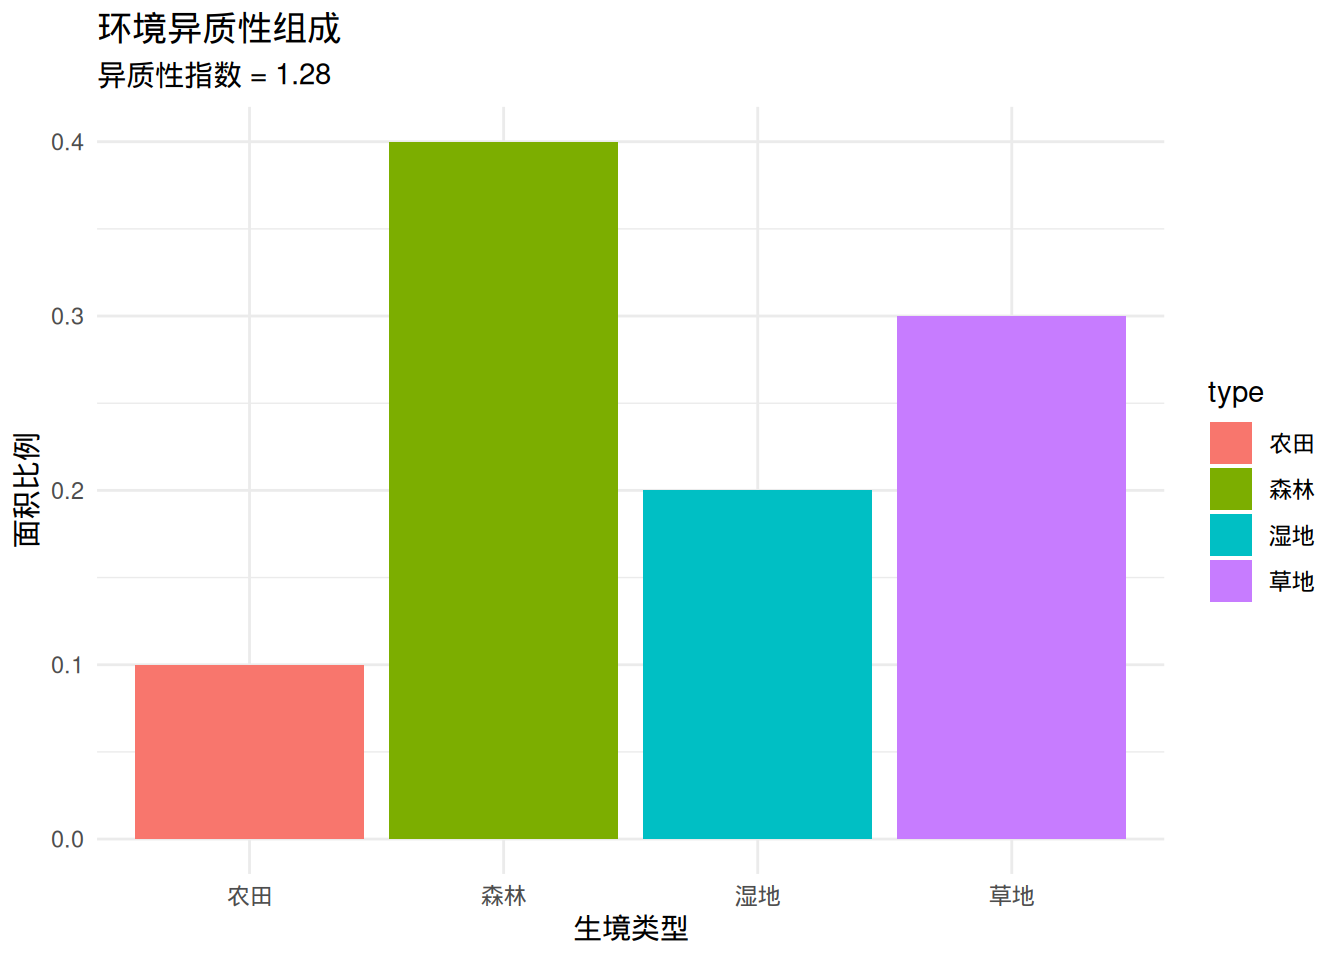
\includegraphics{02-probability_and_distribution_files/figure-latex/unnamed-chunk-19-1} 

}

\caption{蚱蜢午餐选择的累积概率分布:阶梯函数展示概率的累积过程}\label{fig:unnamed-chunk-19}
\end{figure}

累积概率分布图呈现为阶梯函数,在每个可能的取值处跳跃,跳跃的高度等于该取值的概率。这种分布特别有用,因为它:

\begin{enumerate}
\def\labelenumi{\arabic{enumi}.}
\tightlist
\item
  \textbf{回答区间概率问题}:我们可以直接读出 P(X ≤ 2) = 0.93\\
\item
  \textbf{计算任意事件的概率}:P(X \textgreater{} 2) = 1 - P(X ≤ 2) = 1 - 0.93 = 0.07\\
\item
  \textbf{提供决策支持}:如果我们想知道''蚱蜢选择营养价值较高的植物(黑麦草或混合草甸)的概率'',累积分布直接给出了答案:0.93
\end{enumerate}

在生态学中,累积概率分布广泛应用于风险评估、资源分配决策和种群管理策略制定。

R语言中的概率分布函数家族

R为各种概率分布提供了完整的函数家族,每个分布都包含四类核心函数:
- d\emph{: 概率密度/质量函数 (density) - 计算特定取值的概率密度或质量\\
- p}: 累积分布函数 (probability) - 计算小于等于某值的累积概率\\
- q\emph{: 分位数函数 (quantile) - 根据概率值反推对应的分位数\\
- r}: 随机数生成函数 (random) - 从该分布中生成随机样本

例如,对于正态分布:
dnorm(x, mean, sd) \# 概率密度函数 - 计算x处的概率密度\\
pnorm(q, mean, sd) \# 累积分布函数 - 计算P(X ≤ q)的概率\\
qnorm(p, mean, sd) \# 分位数函数 - 计算累积概率为p时的分位数\\
rnorm(n, mean, sd) \# 随机数生成 - 生成n个服从正态分布的随机数

这种统一的命名约定使得在R中学习和使用各种分布变得非常直观。生态学家可以轻松地进行概率计算、统计推断和随机模拟。

\begin{longtable}[]{@{}
  >{\raggedright\arraybackslash}p{(\columnwidth - 6\tabcolsep) * \real{0.2500}}
  >{\raggedright\arraybackslash}p{(\columnwidth - 6\tabcolsep) * \real{0.2500}}
  >{\raggedright\arraybackslash}p{(\columnwidth - 6\tabcolsep) * \real{0.2500}}
  >{\raggedright\arraybackslash}p{(\columnwidth - 6\tabcolsep) * \real{0.2500}}@{}}
\toprule\noalign{}
\begin{minipage}[b]{\linewidth}\raggedright
分布类型
\end{minipage} & \begin{minipage}[b]{\linewidth}\raggedright
生态学应用场景
\end{minipage} & \begin{minipage}[b]{\linewidth}\raggedright
R函数前缀
\end{minipage} & \begin{minipage}[b]{\linewidth}\raggedright
主要参数
\end{minipage} \\
\midrule\noalign{}
\endhead
\bottomrule\noalign{}
\endlastfoot
二元选择分布 & 生物行为的是/否决策 & \texttt{binom} & 试验次数、成功概率 \\
计数分布 & 种群数量、事件发生次数 & \texttt{pois} & 平均发生率 \\
等待时间分布 & 生物事件间隔时间 & \texttt{geom}, \texttt{nbinom} & 成功概率、目标次数 \\
多元选择分布 & 多物种竞争、资源分配 & \texttt{multinom} & 试验次数、各类概率 \\
连续分布 & 生物体尺寸、环境变量 & \texttt{norm}, \texttt{unif} & 均值、标准差等 \\
\end{longtable}

这些分布函数为生态学研究提供了强大的数学工具,帮助我们量化自然界的随机现象。

\hypertarget{ux5348ux9910ux83dcux5355ux79bbux6563ux968fux673aux53d8ux91cfux7684ux5206ux5e03ux5bb6ux65cf}{%
\section{午餐菜单:离散随机变量的分布家族}\label{ux5348ux9910ux83dcux5355ux79bbux6563ux968fux673aux53d8ux91cfux7684ux5206ux5e03ux5bb6ux65cf}}

我们已经成功地为蚱蜢的午餐偏好创建了一个数学模型。我们定义了一个随机变量X,它就像一个聪明的代理人,将``吃哪种植物''这个文字问题,转化成了``X等于1,2,还是3?''这个数学问题。

离散型随机变量的核心特征就是:它的可能取值是有限个或可数的无限个(就像整数一样,可以一个一个数出来)。蚱蜢的选择(1,2,3)就是有限的、分立的点,而不是连续的光滑区间。我们整理出的那张概率表格,正是这个随机变量的概率分布。它如同一份``行为密码'',精确地告诉我们这只蚱蜢的习性。

不过,自然界的奥秘在于,许多看似不同的行为背后,可能隐藏着同一种``底层法则''。接下来,就让我们认识几位在生态学中无处不在的离散分布``明星''。

\hypertarget{ux4f2fux52aaux5229ux5206ux5e03ux4e00ux4e2aux662fux6216ux5426ux7684ux7ec8ux6781ux95eeux9898}{%
\subsection{伯努利分布:一个''是''或''否''的终极问题}\label{ux4f2fux52aaux5229ux5206ux5e03ux4e00ux4e2aux662fux6216ux5426ux7684ux7ec8ux6781ux95eeux9898}}

\textbf{故事开端:} 现在,我不再关心蚱蜢具体吃了三种植物中的哪一种,而是问一个更简单的问题:它这次进食是否选择了黑麦草? 结果只有两种:``是''(成功) 或 ``否''(失败)。这种简化的视角让我们能够专注于最本质的二元选择问题。

\textbf{数学定义:} 伯努利分布是描述单次伯努利试验结果的概率分布。伯努利试验具有三个基本特征:
1. 每次试验只有两种可能的结果(成功/失败)
2. 每次试验中成功的概率\(p\)保持不变
3. 各次试验相互独立

\textbf{概率函数表达式:} 伯努利分布的概率质量函数为:

\[P(X = x) = \begin{cases}
p & \text{如果 } x = 1 \\
1-p & \text{如果 } x = 0
\end{cases}\]

或者更简洁地表示为:
\[P(X = x) = p^x(1-p)^{1-x}, \quad x = 0,1\]

其中,\(X\)是伯努利随机变量,\(p\)是成功的概率(\(0 \leq p \leq 1\))。

\begin{figure}

{\centering \includegraphics{02-probability_and_distribution_files/figure-latex/unnamed-chunk-20-1} 

}

\caption{伯努利分布:不同成功概率下的二元选择概率分布}\label{fig:unnamed-chunk-20}
\end{figure}

\textbf{生态学肖像:}

伯努利分布在生态学中无处不在,它描述的是那些具有二元结局的自然现象。在生态系统的各个层面,我们都能观察到这种简单的二元选择模式:一颗种子是否发芽,一只雏鸟能否成功活到离巢,一次野外调查中样方里是否出现目标物种,一只昆虫是否被天敌捕食,或者一片叶子是否被昆虫取食。这些看似简单的''是''或''否''问题,实际上构成了生态学中最基本的概率单元。

\textbf{生态学意义:}

伯努利分布虽然简单,但它是构建更复杂生态学模型的基础。许多重要的生态学分布,如二项分布、几何分布、负二项分布等,都是建立在多次独立伯努利试验的基础之上。理解伯努利分布有助于我们量化二元生态过程,将定性的生态现象转化为可量化的概率;建立基准模型,为更复杂的生态模型提供理论基础;进行统计推断,基于二元数据估计生态过程的参数;以及评估生态事件发生的可能性。

伯努利分布的美妙之处在于它的简洁性和普适性。尽管生态系统的复杂性远超简单的二元选择,但通过将复杂问题分解为基本的伯努利试验,我们能够逐步建立起理解自然界的数学模型框架。

\hypertarget{ux4e8cux9879ux5206ux5e03ux91cdux590dux662fux975eux9898ux7684ux8ba1ux6570ux6cd5ux5219}{%
\subsection{二项分布:重复''是非题''的计数法则}\label{ux4e8cux9879ux5206ux5e03ux91cdux590dux662fux975eux9898ux7684ux8ba1ux6570ux6cd5ux5219}}

\textbf{故事延续:} 现在,我连续观察蚱蜢的10次进食选择。每一次选择,都是一个独立的伯努利试验(是否吃黑麦草)。我关心的问题是:在这10次观察中,它总共有多大概率有恰好7次选择了黑麦草?或者,至少有8次?这种从单次试验扩展到多次试验的视角,引导我们认识二项分布。

\textbf{数学定义:} 二项分布描述的是在\(n\)次独立的伯努利试验中,成功次数\(k\)的概率分布。二项试验满足以下条件:
1. 试验由\(n\)次相同的伯努利试验组成
2. 每次试验只有两种可能的结果(成功/失败)
3. 每次试验的成功概率\(p\)保持不变
4. 各次试验相互独立

\textbf{概率函数表达式:} 二项分布的概率质量函数为:

\[P(X = k) = \binom{n}{k} p^k (1-p)^{n-k}, \quad k = 0, 1, 2, \ldots, n\]

其中:
- \(X\)是二项随机变量,表示成功的次数
- \(n\)是试验总次数
- \(k\)是成功次数
- \(p\)是每次试验的成功概率
- \(\binom{n}{k} = \frac{n!}{k!(n-k)!}\)是二项系数

\textbf{分布特性:}
- 期望值:\(E[X] = np\)
- 方差:\(Var(X) = np(1-p)\)
- 当\(p=0.5\)时,分布对称;当\(p<0.5\)时右偏,\(p>0.5\)时左偏

\begin{figure}

{\centering \includegraphics{02-probability_and_distribution_files/figure-latex/unnamed-chunk-21-1} 

}

\caption{二项分布:不同成功概率下多次试验中成功次数的概率分布}\label{fig:unnamed-chunk-21}
\end{figure}

\textbf{生态学肖像:}

二项分布在生态学中广泛应用于计数型数据的建模。当我们播种100颗同种种子时,最终成功发芽的数量\(k\)服从二项分布,其中\(n=100\),\(p\)代表种子的发芽率。从一个大种群中随机捕获并标记50只动物,放回后再次随机捕获50只,其中被标记个体的数量\(k\)也服从二项分布,这正是标记重捕法的理论核心。在一片森林中,随机选择的100棵树中有病害的树木数量同样遵循二项分布规律。一次生态调查中,在50个样方中发现目标物种的样方数量,以及一个鸟类种群中在繁殖季节成功孵化的雏鸟数量,都可以用二项分布来精确描述。

\textbf{生态学意义:}

二项分布是伯努利分布的自然延伸,它将单个二元事件的概率模型扩展到多个独立事件的计数模型。在生态学研究中,二项分布帮助我们进行种群估计,通过标记重捕法精确估计种群大小;支持患病率研究,准确估计疾病在种群中的传播程度;实现物种分布量化,精确描述物种在特定区域的分布概率;评估繁殖成功率,科学衡量物种的繁殖表现;以及优化抽样设计,合理确定生态调查的样本大小。二项分布的美妙之处在于它将复杂的生态计数问题简化为基本的概率计算,为我们提供了量化生态现象的有力工具。

\hypertarget{ux591aux9879ux5f0fux5206ux5e03ux591aux5143ux9009ux62e9ux7684ux5168ux666fux56fe}{%
\subsection{多项式分布:多元选择的''全景图''}\label{ux591aux9879ux5f0fux5206ux5e03ux591aux5143ux9009ux62e9ux7684ux5168ux666fux56fe}}

\textbf{故事视角扩展:} 二项分布处理的是''是/否''的二元选择,但生态学中我们常常面临更复杂的多元选择。回到蚱蜢的午餐选择,现在我想知道:在10次进食观察中,它恰好有6次选择黑麦草、3次选择混合草甸、1次选择三叶草的概率是多少?这种对多个类别同时计数的需求,引导我们认识多项式分布。

\textbf{数学定义:} 多项式分布是二项分布向多个类别的自然推广,描述的是在\(n\)次独立试验中,每个类别出现特定次数的联合概率分布。多项式试验满足以下条件:
1. 每次试验有\(k\)个可能的结果(类别)
2. 每个结果发生的概率分别为\(p_1, p_2, \ldots, p_k\),且\(\sum_{i=1}^k p_i = 1\)
3. 各次试验相互独立
4. 试验结果互斥且完备

\textbf{概率函数表达式:} 多项式分布的概率质量函数为:

\[P(X_1 = x_1, X_2 = x_2, \ldots, X_k = x_k) = \frac{n!}{x_1! x_2! \cdots x_k!} p_1^{x_1} p_2^{x_2} \cdots p_k^{x_k}\]

其中:
- \(X_i\)表示第\(i\)个类别出现的次数
- \(x_i\)是第\(i\)个类别的实际观察次数,且\(\sum_{i=1}^k x_i = n\)
- \(n\)是总的试验次数
- \(p_i\)是第\(i\)个类别发生的概率
- \(\frac{n!}{x_1! x_2! \cdots x_k!}\)是多项式系数

\textbf{分布特性:}
- 每个类别的边际分布都是二项分布:\(X_i \sim \text{Binomial}(n, p_i)\)
- 期望值:\(E[X_i] = np_i\)
- 方差:\(Var(X_i) = np_i(1-p_i)\)
- 协方差:\(Cov(X_i, X_j) = -np_i p_j\)(\(i \neq j\))
- 当\(k=2\)时,多项式分布退化为二项分布

\begin{figure}

{\centering \includegraphics{02-probability_and_distribution_files/figure-latex/unnamed-chunk-22-1} 

}

\caption{多项式分布:蚱蜢10次观察中不同植物选择组合的概率分布}\label{fig:unnamed-chunk-22}
\end{figure}

\textbf{生态学肖像:}

多项式分布在生态学中广泛应用于多类别计数数据的建模。一片森林中不同树种幼苗数量的联合分布能够描述植物群落的组成结构;一次鸟类调查中不同物种出现次数的联合概率可以分析鸟类群落的多样性模式;一个湖泊中不同浮游生物类群数量的分布有助于研究水生生态系统的营养结构;一次昆虫采集样本中不同科属昆虫数量的分布能够量化昆虫群落的分类组成;一个动物种群的年龄结构分布则可以分析种群动态的多类别特征。

\textbf{生态学意义:}

多项式分布是生态学中描述多变量计数数据的核心工具,它帮助我们在群落生态学中量化物种组成的联合概率分布,在多样性研究中分析多物种共存模式的概率特征,在资源分配中研究生物对不同资源的选择偏好,在种群结构中描述年龄、性别等多类别特征的分布,以及在生态监测中设计多变量生态调查的统计框架。多项式分布的美妙之处在于它能够同时捕捉多个生态类别的联合分布模式,为我们理解生态系统的复杂性和多样性提供了全面的数学框架。

\hypertarget{ux6ccaux677eux5206ux5e03ux7f55ux89c1ux4e8bux4ef6ux7684ux4f4eux8bedux8005}{%
\subsection{泊松分布:罕见事件的''低语者''}\label{ux6ccaux677eux5206ux5e03ux7f55ux89c1ux4e8bux4ef6ux7684ux4f4eux8bedux8005}}

\textbf{故事新篇:} 这次,我不固定观察次数,而是固定观察时间。我坐在草地上,用一个小时的时间,记录下这只蚱蜢做出剧烈警戒性跳跃的次数。这种跳跃并不频繁,可能一次,可能两次,也可能一次都没有。在一个很短的时间间隔内,发生一次跳跃的概率很小,且事件彼此独立。这种对稀有事件计数的需求,引导我们认识泊松分布。

\textbf{数学定义:} 泊松分布描述的是在固定时间间隔、固定面积或固定体积内,稀有事件发生次数的概率分布。泊松过程满足以下条件:
1. 事件在任意小的时间间隔内发生的概率与时间间隔长度成正比
2. 在不相交的时间间隔内,事件发生次数相互独立
3. 事件在任意时间点发生的概率相同(平稳性)
4. 在极短时间间隔内,发生两次或以上事件的概率可以忽略

\textbf{概率函数表达式:} 泊松分布的概率质量函数为:

\[P(X = k) = \frac{\lambda^k e^{-\lambda}}{k!}, \quad k = 0, 1, 2, \ldots\]

其中:
- \(X\)是泊松随机变量,表示事件发生的次数
- \(\lambda\)是单位时间(或单位面积/体积)内事件发生的平均次数
- \(k\)是实际观察到的事件次数
- \(e\)是自然对数的底(约等于2.71828)

\textbf{分布特性:}
- 期望值:\(E[X] = \lambda\)
- 方差:\(Var(X) = \lambda\)(期望等于方差是泊松分布的重要特征)
- 当\(\lambda\)较小时,分布右偏;当\(\lambda\)增大时,分布逐渐接近正态分布
- 泊松分布是二项分布在\(n \to \infty\),\(p \to 0\),且\(np = \lambda\)时的极限情况

\begin{figure}

{\centering \includegraphics{02-probability_and_distribution_files/figure-latex/unnamed-chunk-23-1} 

}

\caption{泊松分布:不同平均发生率下稀有事件发生次数的概率分布}\label{fig:unnamed-chunk-23}
\end{figure}

\textbf{生态学肖像:}

泊松分布在生态学中广泛应用于稀有事件和空间分布的研究。一平方米的森林样地中某种珍稀兰花的株数能够描述稀有物种的空间分布模式;一台红外相机在一天内拍摄到某种神秘夜行兽的次数可以监测稀有动物的活动频率;一毫升海水中的浮游生物数量有助于量化微生物的密度分布;一片草原上单位面积内某种昆虫的巢穴数量能够研究昆虫的空间分布模式;一个湖泊中特定时间段内鱼类跃出水面的次数则可以记录稀有行为的发生频率。

\textbf{生态学意义:}

泊松分布是生态学中描述随机分布模式的重要工具,它帮助我们在物种分布研究中判断物种在空间上是否随机分布,通过单位面积内的个体数估计总体密度,在行为生态学中量化稀有行为的发生频率,在保护生物学中评估稀有物种的分布状况,以及在生态监测中设计合理的监测方案和样本大小。

泊松分布的美妙之处在于它用一个简单的参数\(\lambda\)就描述了复杂生态现象的概率规律,为我们理解自然界的随机性提供了简洁而强大的数学工具。

\hypertarget{ux51e0ux4f55ux5206ux5e03ux7b49ux5f85ux7b2cux4e00ux6b21ux6210ux529fux7684ux8010ux5fc3}{%
\subsection{几何分布:等待''第一次成功''的耐心}\label{ux51e0ux4f55ux5206ux5e03ux7b49ux5f85ux7b2cux4e00ux6b21ux6210ux529fux7684ux8010ux5fc3}}

\textbf{故事视角转换:} 想象现在是清晨,蚱蜢开始了它的第一次觅食。我好奇的是:它需要尝试多少次,才能第一次成功吃到它最爱的黑麦草? 也许第一次就成功了(X=1),也许前两次都去了别处,第三次才成功(X=3)。这种对''第一次成功''等待时间的关注,引导我们认识几何分布。

\textbf{数学定义:} 几何分布描述的是在一系列独立的伯努利试验中,首次获得成功所需要的试验次数。几何分布满足以下条件:
1. 试验由一系列相同的伯努利试验组成
2. 每次试验只有两种可能的结果(成功/失败)
3. 每次试验的成功概率\(p\)保持不变
4. 各次试验相互独立
5. 试验持续进行直到第一次成功出现

\textbf{概率函数表达式:} 几何分布的概率质量函数为:

\[P(X = k) = (1-p)^{k-1} p, \quad k = 1, 2, 3, \ldots\]

其中:
- \(X\)是几何随机变量,表示首次成功所需的试验次数
- \(k\)是试验次数(\(k \geq 1\))
- \(p\)是每次试验的成功概率
- \((1-p)^{k-1}\)表示前\(k-1\)次都失败的概率

\textbf{分布特性:}
- 期望值:\(E[X] = \frac{1}{p}\)
- 方差:\(Var(X) = \frac{1-p}{p^2}\)
- 无记忆性:\(P(X > m+n \mid X > m) = P(X > n)\),即过去的失败不影响未来的成功概率
- 当\(p\)较小时,分布右偏严重;当\(p\)接近1时,分布集中在较小的\(k\)值

\begin{figure}

{\centering \includegraphics{02-probability_and_distribution_files/figure-latex/unnamed-chunk-24-1} 

}

\caption{几何分布:不同成功概率下首次成功所需试验次数的概率分布}\label{fig:unnamed-chunk-24}
\end{figure}

\textbf{生态学肖像:}

几何分布在生态学中广泛应用于''等待时间''和''首次成功''的研究。一只捕食者需要巡视几个洞穴才能发现第一个有猎物的过程能够描述捕食效率;一只传粉昆虫需要访问多少朵花才能第一次成功获得花蜜有助于研究传粉行为效率;一颗种子需要经历多少个雨季才能第一次成功发芽可以分析种子萌发模式;一只候鸟需要尝试多少次才能第一次成功找到迁徙路线能够研究学习行为;一个植物种群需要经过多少代才能第一次出现抗病突变则有助于分析进化过程。

\textbf{生态学意义:}

几何分布是生态学中描述''等待过程''的重要工具,它帮助我们在行为生态学中量化动物行为的效率和成功率,在种群动态中分析种群恢复和重建的时间过程,在进化生态学中研究适应性特征的进化时间尺度,在保护生物学中评估濒危物种恢复的可能性,以及在生态恢复中预测生态系统恢复所需的时间。

几何分布的美妙之处在于它用一个简单的参数\(p\)就描述了复杂生态过程中的等待时间规律,特别是其''无记忆性''特征,使得我们可以专注于当前的生态过程而不受历史影响。

\hypertarget{ux8d1fux4e8cux9879ux5206ux5e03ux7b49ux5f85ux6700ux540eux4e00ux6b21ux6210ux529fux7684ux8010ux5fc3}{%
\subsection{负二项分布:等待''最后一次成功''的耐心}\label{ux8d1fux4e8cux9879ux5206ux5e03ux7b49ux5f85ux6700ux540eux4e00ux6b21ux6210ux529fux7684ux8010ux5fc3}}

\textbf{故事视角深化:} 几何分布关注的是''第一次成功'',但生态学中我们常常需要更复杂的等待模式。比如,我想知道:这只蚱蜢需要尝试多少次,才能\textbf{第三次}成功吃到黑麦草?这种对''第r次成功''等待时间的关注,引导我们认识负二项分布。

\textbf{数学定义:} 负二项分布描述的是在一系列独立的伯努利试验中,获得第r次成功所需要的试验次数。负二项分布满足以下条件:
1. 试验由一系列相同的伯努利试验组成
2. 每次试验只有两种可能的结果(成功/失败)
3. 每次试验的成功概率\(p\)保持不变
4. 各次试验相互独立
5. 试验持续进行直到第r次成功出现

\textbf{概率函数表达式:} 负二项分布的概率质量函数为:

\[P(X = k) = \binom{k-1}{r-1} p^r (1-p)^{k-r}, \quad k = r, r+1, r+2, \ldots\]

其中:
- \(X\)是负二项随机变量,表示第r次成功所需的试验次数
- \(k\)是总的试验次数(\(k \geq r\))
- \(r\)是期望的成功次数
- \(p\)是每次试验的成功概率
- \(\binom{k-1}{r-1}\)是组合数,表示前\(k-1\)次试验中安排\(r-1\)次成功的方式数

\textbf{分布特性:}
- 期望值:\(E[X] = \frac{r}{p}\)
- 方差:\(Var(X) = \frac{r(1-p)}{p^2}\)
- 当\(r=1\)时,负二项分布退化为几何分布
- 分布形状取决于\(r\)和\(p\)的值,可以呈现不同的偏斜形态

\begin{figure}

{\centering \includegraphics{02-probability_and_distribution_files/figure-latex/unnamed-chunk-25-1} 

}

\caption{负二项分布:不同参数组合下第r次成功所需试验次数的概率分布}\label{fig:unnamed-chunk-25}
\end{figure}

\textbf{生态学肖像:}

负二项分布在生态学中广泛应用于需要多次成功才能达到目标的场景。一只捕食者需要捕获多少只猎物才能满足其能量需求(第r次成功捕食),这描述了捕食效率的累积效应。一个植物种群需要经过多少代才能积累到足够的有利突变(第r次有利突变),这有助于分析进化过程的累积性。一次生态调查需要设置多少个样方才能第r次发现目标稀有物种,这有助于优化稀有物种监测方案。一个生态系统需要经历多少次干扰才会达到第r次显著的结构变化,这有助于研究生态系统的累积响应。一个保护项目需要实施多少项措施才能第r次观察到种群恢复迹象,这有助于评估保护措施的有效性。

\textbf{生态学意义:}

负二项分布是几何分布的自然推广,它将单次成功的等待时间模型扩展到多次成功的累积等待时间模型。在生态学研究中,负二项分布帮助我们:

\begin{enumerate}
\def\labelenumi{\arabic{enumi}.}
\tightlist
\item
  \textbf{资源管理}:预测达到特定资源积累目标所需的时间或努力
\item
  \textbf{种群监测}:设计合理的监测方案来发现稀有物种
\item
  \textbf{保护规划}:评估保护措施实施的时间框架和效果
\item
  \textbf{进化研究}:分析适应性特征积累的时间尺度
\item
  \textbf{风险评估}:评估生态系统达到临界状态所需的干扰次数
\end{enumerate}

负二项分布的美妙之处在于它能够描述生态系统中''累积成功''的复杂模式,为我们理解生态过程的渐进性和累积性提供了有力的数学工具。

\hypertarget{ux5348ux9910ux6cd5ux5219ux8fdeux7eedux968fux673aux53d8ux91cfux7684ux5206ux5e03ux5bb6ux65cf}{%
\section{午餐法则:连续随机变量的分布家族}\label{ux5348ux9910ux6cd5ux5219ux8fdeux7eedux968fux673aux53d8ux91cfux7684ux5206ux5e03ux5bb6ux65cf}}

\textbf{从跳跃到体长:描绘连续世界的概率地图}

我们已经为蚱蜢的''午餐选择''绘制了一张清晰的概率分布图,那是由一根根独立的柱子组成的,因为它的选择是分门别类的(植物A、B、C)。这类变量被称为离散型随机变量,它们的取值是可数的。

但现在,让我们拿起尺子和高速摄像机,关注一些更细微、更流畅的特征。比如,这只蚱蜢的体长是多少厘米?或者它受到惊吓时,一次跳跃的距离是多少米?这些数值,可以是3.15厘米,也可以是3.151厘米,甚至在理论上可以是3.1515926\ldots 厘米。它们的取值充满了无限的可能性,充满了''连续性''。

连续型随机变量的核心特征就是:它的可能取值构成一个连续的区间,无法一一列举。在生态学中,绝大多数测量值都是连续的------温度、湿度、海拔、生物量、生长速率等等。这些变量构成了我们对自然界的量化认知基础。

\textbf{从柱子到光滑的曲线:概率密度函数}

当我们面对这样一个连续型随机变量时,之前那种''给每个特定值分配一个概率''的方法就失效了。因为任何一个精确值的概率(比如P(体长=3.15厘米))在无限的可能性面前,都几乎等于零!这就像问''在一根无限长的线上,恰好选中某个点的概率是多少?``------答案是零。

那么,我们该如何描述它的概率分布呢?聪明的做法是,我们不再关心''点''的概率,而是关心''区间''的概率。我们问的是:``这只蚱蜢的体长在3.1厘米到3.2厘米之间的概率是多少?'' 这时,概率就不再是柱子的高度,而是曲线下某一块区域的面积。

这条至关重要的曲线,就叫做\textbf{概率密度函数} 曲线。曲线本身在任意一点的高度(概率密度)并不直接代表概率,但它决定了概率的大小:曲线越高、越''胖''的区域,对应的区间概率就越大。曲线下的总面积,被定义为1,代表了所有可能性的总和(100\%)。

\textbf{数学定义:} 对于连续随机变量X,其概率密度函数\(f(x)\)满足:

\begin{enumerate}
\def\labelenumi{\arabic{enumi}.}
\tightlist
\item
  非负性:\(f(x) \geq 0\) 对所有\(x\)
\item
  规范性:\(\int_{-\infty}^{\infty} f(x) dx = 1\)
\item
  区间概率:\(P(a \leq X \leq b) = \int_a^b f(x) dx\)
\end{enumerate}

\textbf{累积分布函数:连续世界的''阶梯''}

与离散随机变量类似,连续随机变量也有其累积分布函数,定义为:

\[F(x) = P(X \leq x) = \int_{-\infty}^x f(t) dt\]

累积分布函数\(F(x)\)给出了随机变量取值小于或等于\(x\)的概率。它具有以下重要性质:

\begin{enumerate}
\def\labelenumi{\arabic{enumi}.}
\tightlist
\item
  单调不减:如果\(x_1 < x_2\),则\(F(x_1) \leq F(x_2)\)
\item
  边界条件:\(\lim_{x \to -\infty} F(x) = 0\),\(\lim_{x \to \infty} F(x) = 1\)
\item
  右连续性:\(F(x)\)在任意点\(x\)处右连续
\end{enumerate}

通过累积分布函数,我们可以方便地计算各种概率:
- \(P(a < X \leq b) = F(b) - F(a)\)
- \(P(X > x) = 1 - F(x)\)

\begin{figure}

{\centering \includegraphics{02-probability_and_distribution_files/figure-latex/unnamed-chunk-26-1} 

}

\caption{连续随机变量的概率密度函数与累积分布函数对比}\label{fig:unnamed-chunk-26}
\end{figure}

在连续变量的世界里,有几个声名显赫的''家族'',它们以特定的形态描绘了不同自然现象背后的概率规律。每个分布都有其独特的数学特性和生态学意义,共同构成了我们理解连续生态变量的工具箱。

\hypertarget{ux5747ux5300ux5206ux5e03ux7eafux7cb9ux7684ux5e73ux7b49}{%
\subsection{均匀分布:纯粹的平等}\label{ux5747ux5300ux5206ux5e03ux7eafux7cb9ux7684ux5e73ux7b49}}

\textbf{故事引入:} 想象这只蚱蜢找到了一片巨大且质地均匀的叶子,它准备开始享用午餐。这片叶子从叶尖到叶柄的长度是10厘米。蚱蜢会随机选择一个位置开始进食。它第一口吃的位置到叶尖的距离是多少厘米?可能是2厘米,也可能是5厘米,或者8厘米,每个距离被选中的可能性完全相同。这种''完全随机''的选择过程,就是均匀分布的典型场景。

\textbf{数学定义:} 均匀分布描述的是在区间\([a, b]\)内,所有取值等可能出现的概率分布。其概率密度函数为:

\[f(x) = \begin{cases}
\frac{1}{b-a} & \text{如果 } a \leq x \leq b \\
0 & \text{其他}
\end{cases}\]

\textbf{分布特性:}
- 期望值:\(E[X] = \frac{a+b}{2}\)
- 方差:\(Var(X) = \frac{(b-a)^2}{12}\)
- 在区间\([a, b]\)内,概率密度恒定

\textbf{生态学肖像:}

在生态学研究中,均匀分布具有重要的应用价值。在觅食行为研究中,蚱蜢在均匀资源上的随机选择行为服从均匀分布。当食物资源分布均匀时,动物的觅食位置选择可以建模为均匀分布。在行为生态学实验中,动物的随机选择行为可以用均匀分布来描述,这为理解生物在理想化环境中的决策模式提供了理论基准。

\begin{figure}

{\centering \includegraphics{02-probability_and_distribution_files/figure-latex/unnamed-chunk-27-1} 

}

\caption{均匀分布:不同区间参数下的概率密度函数}\label{fig:unnamed-chunk-27}
\end{figure}

\hypertarget{ux6307ux6570ux5206ux5e03ux7b49ux5f85ux7684ux827aux672f}{%
\subsection{指数分布:等待的艺术}\label{ux6307ux6570ux5206ux5e03ux7b49ux5f85ux7684ux827aux672f}}

\textbf{故事引入:} 现在让我们关注时间维度。这只蚱蜢正在草地上专心享用午餐,但它必须时刻保持警惕。下一次被天敌(如鸟类)发现需要等待多长时间?可能是几分钟,也可能是几十分钟。这种''等待被捕食''的时间间隔,正是指数分布的用武之地。在蚱蜢的午餐过程中,这种生存威胁的随机出现模式可以用指数分布来精确描述。

\textbf{数学定义:} 指数分布描述的是泊松过程中事件发生的时间间隔。其概率密度函数为:

\[f(x) = \lambda e^{-\lambda x}, \quad x \geq 0\]

其中\(\lambda > 0\)是速率参数,表示单位时间内事件发生的平均次数。

\textbf{分布特性:}
- 期望值:\(E[X] = \frac{1}{\lambda}\)
- 方差:\(Var(X) = \frac{1}{\lambda^2}\)
- \textbf{无记忆性}:\(P(X > s + t \mid X > s) = P(X > t)\),即过去的等待不影响未来的等待时间
- 分布呈右偏,具有长尾特征

\textbf{生态学肖像:}

指数分布在生态学中具有广泛的应用价值。在捕食风险建模方面,蚱蜢在觅食过程中被捕食者发现的等待时间服从指数分布,这种分布模式反映了捕食事件的随机性特征。无记忆性这一重要特性为生存策略研究提供了理论基础,它表明过去的等待时间不影响未来的风险概率,这有助于我们深入理解蚱蜢的警戒行为模式。在行为时间模式分析中,动物在危险环境中的活动间隔可以用指数分布来描述,这种分布能够捕捉动物在风险环境中的行为节律。在种群生存分析领域,特别是在高捕食压力环境下,个体的生存时间分布往往近似指数分布,这为种群动态研究和保护策略制定提供了重要的数学工具。

\begin{figure}

{\centering \includegraphics{02-probability_and_distribution_files/figure-latex/unnamed-chunk-28-1} 

}

\caption{指数分布:不同速率参数下等待时间的概率密度函数}\label{fig:unnamed-chunk-28}
\end{figure}

\hypertarget{ux6b63ux6001ux5206ux5e03ux9ad8ux65afux5206ux5e03ux81eaux7136ux754cux7684ux949fux5f62ux6cd5ux5219}{%
\subsection{正态分布(高斯分布):自然界的''钟形''法则}\label{ux6b63ux6001ux5206ux5e03ux9ad8ux65afux5206ux5e03ux81eaux7136ux754cux7684ux949fux5f62ux6cd5ux5219}}

\textbf{故事引入:} 仔细观察这只蚱蜢的午餐习惯,你会发现每次它吃的食物量(如叶片面积或花蜜量)存在自然的变异。大部分情况下,它吃的量都集中在某个平均值附近,极端过多或过少的摄食行为相对少见。这种''中间多,两头少''的分布模式,就是正态分布的典型特征。蚱蜢的摄食行为受到多种微小因素的共同影响,最终呈现出这种经典的钟形分布。

\textbf{数学定义:} 正态分布的概率密度函数为:

\[f(x) = \frac{1}{\sqrt{2\pi}\sigma} e^{-\frac{(x-\mu)^2}{2\sigma^2}}, \quad -\infty < x < \infty\]

其中\(\mu\)是均值(决定分布的中心位置),\(\sigma\)是标准差(决定分布的离散程度)。

\textbf{分布特性:}
- 期望值:\(E[X] = \mu\)
- 方差:\(Var(X) = \sigma^2\)
- 对称性:分布关于均值\(\mu\)对称
- 68-95-99.7法则:约68\%的数据落在\(\mu \pm \sigma\)内,95\%落在\(\mu \pm 2\sigma\)内,99.7\%落在\(\mu \pm 3\sigma\)内
- 中心极限定理:大量独立随机变量的和近似服从正态分布

\textbf{生态学肖像:}

正态分布在生态学研究中扮演着重要角色。在摄食行为研究中,蚱蜢每次进食的食物量服从正态分布,这种分布模式反映了其稳定的摄食行为特征和生理调节机制。通过营养摄入分析,我们可以利用正态分布来描述个体间的摄食量差异,这种差异模式有助于理解种群内部的资源分配和竞争关系。在行为生态学领域,动物的许多连续行为特征,如觅食时间、移动距离等,往往近似正态分布,这为行为模式的量化分析提供了数学基础。在种群能量学研究中,通过摄食量的正态分布特征,我们可以更准确地估计种群的能量摄入模式,为生态系统能量流动研究提供重要依据。

\begin{figure}

{\centering 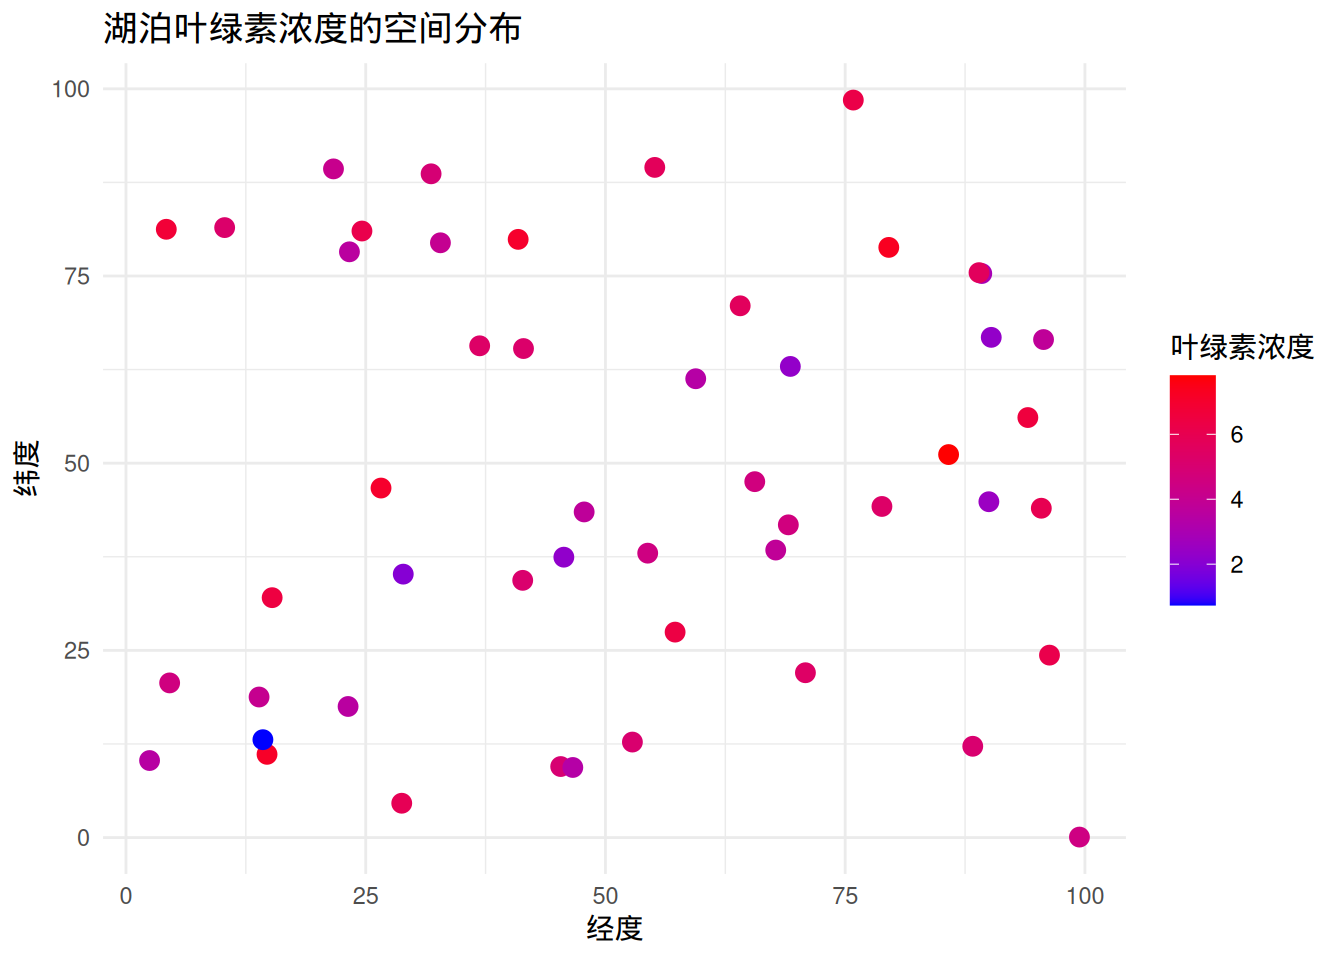
\includegraphics{02-probability_and_distribution_files/figure-latex/unnamed-chunk-29-1} 

}

\caption{正态分布:不同参数组合下的概率密度函数}\label{fig:unnamed-chunk-29}
\end{figure}

\hypertarget{ux5a01ux5e03ux5c14ux5206ux5e03ux751fux5b58ux5206ux6790ux7684ux65f6ux95f4ux6cd5ux5219}{%
\subsection{威布尔分布:生存分析的''时间法则''}\label{ux5a01ux5e03ux5c14ux5206ux5e03ux751fux5b58ux5206ux6790ux7684ux65f6ux95f4ux6cd5ux5219}}

\textbf{故事引入:} 观察这只蚱蜢的生存历程,你会发现它的死亡风险并非一成不变。在生命的早期,由于适应环境的能力较弱,死亡风险相对较高;进入成年期后,风险逐渐稳定;而到了老年期,由于生理机能衰退,死亡风险又会显著上升。这种随时间变化的死亡风险模式,正是威布尔分布能够精确描述的。蚱蜢的生存时间受到多种风险因素的综合影响,最终呈现出这种''浴盆曲线''的风险特征。

\textbf{数学定义:} 威布尔分布的概率密度函数为:

\[f(x) = \frac{k}{\lambda} \left(\frac{x}{\lambda}\right)^{k-1} e^{-(x/\lambda)^k}, \quad x \geq 0\]

其中\(k\)是形状参数(决定分布形态),\(\lambda\)是尺度参数(决定分布范围)。

\textbf{分布特性:}
- 期望值:\(E[X] = \lambda \Gamma(1 + 1/k)\)
- 方差:\(Var(X) = \lambda^2 [\Gamma(1 + 2/k) - \Gamma^2(1 + 1/k)]\)
- 生存函数:\(S(x) = e^{-(x/\lambda)^k}\)
- 风险函数:\(h(x) = \frac{k}{\lambda} \left(\frac{x}{\lambda}\right)^{k-1}\)
- 当\(k=1\)时退化为指数分布(恒定风险)
- 当\(k>1\)时风险随时间增加(老化效应)
- 当\(k<1\)时风险随时间减少(早期适应期)

\textbf{生态学肖像:}

威布尔分布在生态学研究中具有重要的应用价值。在生存分析研究中,蚱蜢的生存时间服从威布尔分布,这种分布能够精确反映其生命周期中风险变化的动态模式,包括早期适应期的高风险和老年期的生理衰退。通过威布尔分布,我们可以在种群动态建模中更准确地估计种群的死亡率模式和期望寿命,为种群管理提供科学依据。在保护生物学领域,濒危物种的生存时间分析有助于制定有效的保护策略,威布尔分布的风险函数能够揭示不同生命阶段的保护重点。此外,在物候学研究中,植物开花时间、动物迁徙时间等时间事件的分析也可以借助威布尔分布来描述其时间分布特征。

\begin{Shaded}
\begin{Highlighting}[]
\CommentTok{\# 威布尔分布:生存分析和寿命数据的分布}
\CommentTok{\# 威布尔分布是生态学中用于生存分析和寿命数据建模的重要工具}
\CommentTok{\# 生态学应用场景:动物寿命分析、设备故障时间预测、种子萌发时间研究等}

\CommentTok{\# 参数设置:定义威布尔分布的两个关键参数}
\CommentTok{\# 形状参数k:决定分布形态和风险函数的变化趋势}
\CommentTok{\# 尺度参数λ:决定分布的范围和尺度}
\NormalTok{shape\_param }\OtherTok{\textless{}{-}} \FloatTok{2.5}  \CommentTok{\# 形状参数大于1表示风险随时间增加(老化效应)}
\NormalTok{scale\_param }\OtherTok{\textless{}{-}} \DecValTok{10}   \CommentTok{\# 尺度参数决定分布的中心位置和范围}

\CommentTok{\# 模拟蚱蜢生存时间数据:从威布尔分布中生成随机样本}
\CommentTok{\# 使用rweibull函数生成200个服从威布尔分布的生存时间观测值}
\CommentTok{\# 这些数据模拟了蚱蜢种群中个体生存时间的自然变异}
\NormalTok{survival\_times }\OtherTok{\textless{}{-}} \FunctionTok{rweibull}\NormalTok{(}\DecValTok{200}\NormalTok{, }\AttributeTok{shape =}\NormalTok{ shape\_param, }\AttributeTok{scale =}\NormalTok{ scale\_param)}
\end{Highlighting}
\end{Shaded}

\begin{Shaded}
\begin{Highlighting}[]
\CommentTok{\# 描述统计:计算样本数据的描述性统计量}
\CommentTok{\# 样本均值:反映蚱蜢生存时间的平均水平}
\FunctionTok{print}\NormalTok{(}\FunctionTok{paste}\NormalTok{(}\StringTok{"样本均值:"}\NormalTok{, }\FunctionTok{round}\NormalTok{(}\FunctionTok{mean}\NormalTok{(survival\_times), }\DecValTok{2}\NormalTok{)))}
\end{Highlighting}
\end{Shaded}

\begin{verbatim}
## [1] "样本均值: 9.37"
\end{verbatim}

\begin{Shaded}
\begin{Highlighting}[]
\CommentTok{\# 样本标准差:反映生存时间的变异程度}
\FunctionTok{print}\NormalTok{(}\FunctionTok{paste}\NormalTok{(}\StringTok{"样本标准差:"}\NormalTok{, }\FunctionTok{round}\NormalTok{(}\FunctionTok{sd}\NormalTok{(survival\_times), }\DecValTok{2}\NormalTok{)))}
\end{Highlighting}
\end{Shaded}

\begin{verbatim}
## [1] "样本标准差: 3.84"
\end{verbatim}

\begin{Shaded}
\begin{Highlighting}[]
\CommentTok{\# 理论均值和方差计算:基于威布尔分布的数学公式}
\CommentTok{\# 威布尔分布的均值和方差公式:}
\CommentTok{\# 期望值 E[X] = λΓ(1 + 1/k),其中Γ是伽马函数}
\CommentTok{\# 方差 Var(X) = λ²[Γ(1 + 2/k) {-} Γ²(1 + 1/k)]}
\CommentTok{\# 这些公式提供了理论基准,用于验证模拟数据的准确性}

\CommentTok{\# 计算理论均值:使用伽马函数计算威布尔分布的期望值}
\NormalTok{theoretical\_mean }\OtherTok{\textless{}{-}}\NormalTok{ scale\_param }\SpecialCharTok{*} \FunctionTok{gamma}\NormalTok{(}\DecValTok{1} \SpecialCharTok{+} \DecValTok{1} \SpecialCharTok{/}\NormalTok{ shape\_param)}
\CommentTok{\# 计算理论方差:使用伽马函数计算威布尔分布的方差}
\NormalTok{theoretical\_var }\OtherTok{\textless{}{-}}\NormalTok{ scale\_param}\SpecialCharTok{\^{}}\DecValTok{2} \SpecialCharTok{*}\NormalTok{ (}\FunctionTok{gamma}\NormalTok{(}\DecValTok{1} \SpecialCharTok{+} \DecValTok{2} \SpecialCharTok{/}\NormalTok{ shape\_param) }\SpecialCharTok{{-}}
                                   \FunctionTok{gamma}\NormalTok{(}\DecValTok{1} \SpecialCharTok{+} \DecValTok{1} \SpecialCharTok{/}\NormalTok{ shape\_param)}\SpecialCharTok{\^{}}\DecValTok{2}\NormalTok{)}

\CommentTok{\# 输出理论计算结果:与样本统计量进行比较}
\FunctionTok{print}\NormalTok{(}\FunctionTok{paste}\NormalTok{(}\StringTok{"理论均值:"}\NormalTok{, }\FunctionTok{round}\NormalTok{(theoretical\_mean, }\DecValTok{2}\NormalTok{)))}
\end{Highlighting}
\end{Shaded}

\begin{verbatim}
## [1] "理论均值: 8.87"
\end{verbatim}

\begin{Shaded}
\begin{Highlighting}[]
\FunctionTok{print}\NormalTok{(}\FunctionTok{paste}\NormalTok{(}\StringTok{"理论方差:"}\NormalTok{, }\FunctionTok{round}\NormalTok{(theoretical\_var, }\DecValTok{2}\NormalTok{)))}
\end{Highlighting}
\end{Shaded}

\begin{verbatim}
## [1] "理论方差: 14.41"
\end{verbatim}

\begin{Shaded}
\begin{Highlighting}[]
\CommentTok{\# 威布尔分布可视化:绘制直方图和理论曲线对比}
\CommentTok{\# 使用基础R绘图系统创建生存时间分布的直方图}
\CommentTok{\# 设置直方图参数:30个分箱,显示密度而非频数}
\FunctionTok{hist}\NormalTok{(survival\_times,}
  \AttributeTok{breaks =} \DecValTok{30}\NormalTok{, }\AttributeTok{freq =} \ConstantTok{FALSE}\NormalTok{,  }\CommentTok{\# 30个分箱确保分布细节清晰显示}
  \AttributeTok{main =} \StringTok{"蚱蜢生存时间分布(威布尔分布)"}\NormalTok{,  }\CommentTok{\# 图形标题}
  \AttributeTok{xlab =} \StringTok{"生存时间(天)"}\NormalTok{, }\AttributeTok{ylab =} \StringTok{"密度"}\NormalTok{,  }\CommentTok{\# 坐标轴标签}
  \AttributeTok{col =} \StringTok{"lightblue"}\NormalTok{, }\AttributeTok{xlim =} \FunctionTok{c}\NormalTok{(}\DecValTok{0}\NormalTok{, }\DecValTok{25}\NormalTok{)  }\CommentTok{\# 浅蓝色填充,x轴范围覆盖主要生存时间}
\NormalTok{)}

\CommentTok{\# 添加理论威布尔曲线:在直方图上叠加理论概率密度函数}
\CommentTok{\# 生成x轴坐标序列:从0到25天,步长为0.1天}
\NormalTok{x\_vals }\OtherTok{\textless{}{-}} \FunctionTok{seq}\NormalTok{(}\DecValTok{0}\NormalTok{, }\DecValTok{25}\NormalTok{, }\FloatTok{0.1}\NormalTok{)  }\CommentTok{\# 创建密集的x值序列确保理论曲线平滑显示}
\CommentTok{\# 计算理论威布尔分布概率密度:使用dweibull函数}
\CommentTok{\# 基于设定的形状参数和尺度参数计算每个x值的概率密度}
\NormalTok{y\_vals }\OtherTok{\textless{}{-}} \FunctionTok{dweibull}\NormalTok{(x\_vals, }\AttributeTok{shape =}\NormalTok{ shape\_param, }\AttributeTok{scale =}\NormalTok{ scale\_param)  }\CommentTok{\# 计算理论概率密度值}
\CommentTok{\# 绘制理论概率密度曲线:红色实线,线宽为2}
\FunctionTok{lines}\NormalTok{(x\_vals, y\_vals, }\AttributeTok{col =} \StringTok{"red"}\NormalTok{, }\AttributeTok{lwd =} \DecValTok{2}\NormalTok{)  }\CommentTok{\# 红色实线突出理论分布与观测数据的对比}

\CommentTok{\# 添加生存函数曲线:显示个体生存概率随时间的变化}
\CommentTok{\# 计算生存函数值:1减去累积分布函数,表示生存概率}
\NormalTok{survival\_vals }\OtherTok{\textless{}{-}} \DecValTok{1} \SpecialCharTok{{-}} \FunctionTok{pweibull}\NormalTok{(x\_vals, }\AttributeTok{shape =}\NormalTok{ shape\_param, }\AttributeTok{scale =}\NormalTok{ scale\_param)}
\CommentTok{\# 绘制生存函数曲线:蓝色虚线,线宽为2}
\FunctionTok{lines}\NormalTok{(x\_vals, survival\_vals, }\AttributeTok{col =} \StringTok{"blue"}\NormalTok{, }\AttributeTok{lwd =} \DecValTok{2}\NormalTok{, }\AttributeTok{lty =} \DecValTok{2}\NormalTok{)}

\CommentTok{\# 添加图例:说明红色曲线为概率密度,蓝色曲线为生存函数}
\FunctionTok{legend}\NormalTok{(}\StringTok{"topright"}\NormalTok{,}
  \AttributeTok{legend =} \FunctionTok{c}\NormalTok{(}\StringTok{"概率密度"}\NormalTok{, }\StringTok{"生存函数"}\NormalTok{),  }\CommentTok{\# 图例标签明确区分两种曲线含义}
  \AttributeTok{col =} \FunctionTok{c}\NormalTok{(}\StringTok{"red"}\NormalTok{, }\StringTok{"blue"}\NormalTok{), }\AttributeTok{lty =} \DecValTok{1}\SpecialCharTok{:}\DecValTok{2}\NormalTok{, }\AttributeTok{lwd =} \DecValTok{2}  \CommentTok{\# 颜色和线型设置与曲线保持一致}
\NormalTok{)}
\end{Highlighting}
\end{Shaded}

\begin{figure}

{\centering 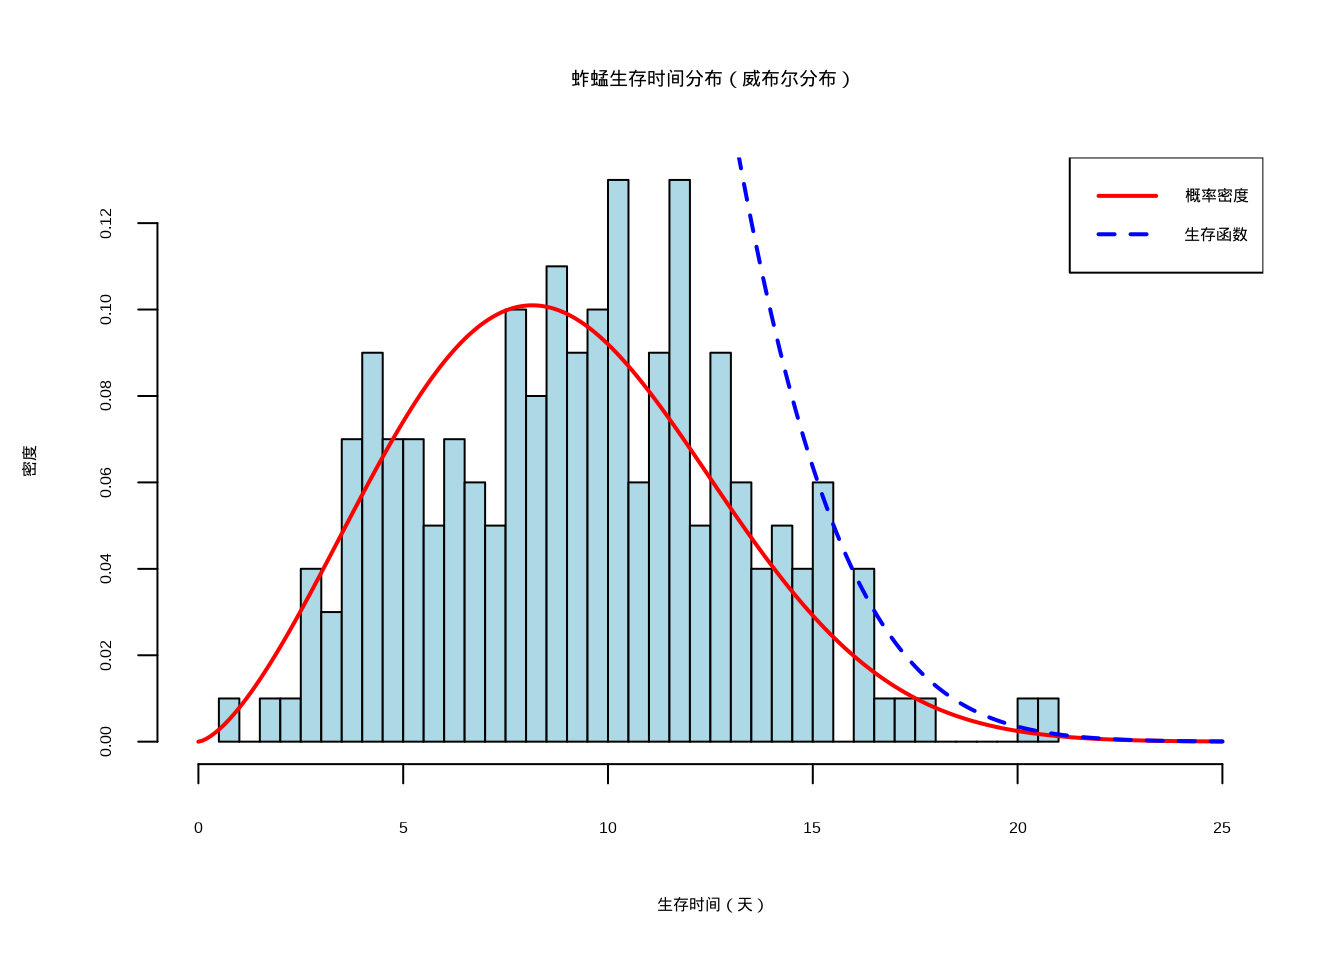
\includegraphics{02-probability_and_distribution_files/figure-latex/unnamed-chunk-32-1} 

}

\caption{威布尔分布可视化:蚱蜢生存时间分布的直方图与理论曲线对比}\label{fig:unnamed-chunk-32}
\end{figure}

\begin{Shaded}
\begin{Highlighting}[]
\CommentTok{\# 参数估计:使用最大似然估计拟合威布尔分布}
\CommentTok{\# 加载fitdistrplus包:提供分布拟合和参数估计功能}
\CommentTok{\# 该包专门用于概率分布的参数估计和拟合优度评估}
\FunctionTok{library}\NormalTok{(fitdistrplus)  }\CommentTok{\# 加载fitdistrplus包用于最大似然估计和分布拟合}

\CommentTok{\# 使用最大似然估计拟合威布尔分布到生存时间数据}
\CommentTok{\# fitdist函数自动估计威布尔分布的形状参数和尺度参数}
\CommentTok{\# 基于模拟的生存时间数据寻找最优参数组合}
\NormalTok{fit\_weibull }\OtherTok{\textless{}{-}} \FunctionTok{fitdist}\NormalTok{(survival\_times, }\StringTok{"weibull"}\NormalTok{)  }\CommentTok{\# 拟合威布尔分布到生存时间数据}

\CommentTok{\# 输出参数估计结果:显示拟合的威布尔分布参数和统计信息}
\FunctionTok{print}\NormalTok{(}\StringTok{"威布尔分布参数估计结果:"}\NormalTok{)  }\CommentTok{\# 打印结果标题便于识别输出内容}
\end{Highlighting}
\end{Shaded}

\begin{verbatim}
## [1] "威布尔分布参数估计结果:"
\end{verbatim}

\begin{Shaded}
\begin{Highlighting}[]
\CommentTok{\# summary函数提供详细的拟合结果,包括参数估计值、标准误、置信区间等}
\FunctionTok{print}\NormalTok{(}\FunctionTok{summary}\NormalTok{(fit\_weibull))  }\CommentTok{\# 输出完整的拟合结果摘要信息}
\end{Highlighting}
\end{Shaded}

\begin{verbatim}
## Fitting of the distribution ' weibull ' by maximum likelihood 
## Parameters : 
##        estimate Std. Error
## shape  2.647722  0.1480560
## scale 10.549286  0.2962823
## Loglikelihood:  -549.6808   AIC:  1103.362   BIC:  1109.958 
## Correlation matrix:
##           shape     scale
## shape 1.0000000 0.3095952
## scale 0.3095952 1.0000000
\end{verbatim}

\begin{Shaded}
\begin{Highlighting}[]
\CommentTok{\# 比较不同形状参数的威布尔分布}
\CommentTok{\# 设置图形布局:创建2x2的多图面板,便于同时比较四种不同形状参数}
\FunctionTok{par}\NormalTok{(}\AttributeTok{mfrow =} \FunctionTok{c}\NormalTok{(}\DecValTok{2}\NormalTok{, }\DecValTok{2}\NormalTok{))  }\CommentTok{\# 2行2列的图形布局,总共显示4个子图}

\CommentTok{\# 定义要比较的形状参数值:展示不同风险模式}
\CommentTok{\# k\textless{}1表示早期风险高(适应期),k=1表示恒定风险(指数分布)}
\CommentTok{\# k\textgreater{}1表示风险随时间增加(老化效应)}
\NormalTok{shape\_values }\OtherTok{\textless{}{-}} \FunctionTok{c}\NormalTok{(}\FloatTok{0.5}\NormalTok{, }\DecValTok{1}\NormalTok{, }\DecValTok{2}\NormalTok{, }\DecValTok{3}\NormalTok{)  }\CommentTok{\# 形状参数k的四种取值:0.5(早期风险高), 1(恒定风险), 2(中等增加), 3(快速增加)}
\NormalTok{scale\_fixed }\OtherTok{\textless{}{-}} \DecValTok{10}  \CommentTok{\# 固定尺度参数λ为10,便于比较形状参数的影响}

\CommentTok{\# 循环遍历所有形状参数值,为每个参数创建概率密度和风险函数图}
\ControlFlowTok{for}\NormalTok{ (shape\_val }\ControlFlowTok{in}\NormalTok{ shape\_values) \{}
  \CommentTok{\# 生成x轴坐标序列:从0到25天,步长为0.1天}
\NormalTok{  x\_range }\OtherTok{\textless{}{-}} \FunctionTok{seq}\NormalTok{(}\DecValTok{0}\NormalTok{, }\DecValTok{25}\NormalTok{, }\FloatTok{0.1}\NormalTok{)  }\CommentTok{\# 创建密集的x值序列确保曲线平滑显示}
  \CommentTok{\# 计算威布尔分布概率密度函数值:使用dweibull函数}
\NormalTok{  density\_vals }\OtherTok{\textless{}{-}} \FunctionTok{dweibull}\NormalTok{(x\_range, }\AttributeTok{shape =}\NormalTok{ shape\_val, }\AttributeTok{scale =}\NormalTok{ scale\_fixed)  }\CommentTok{\# 计算概率密度值}

  \CommentTok{\# 绘制概率密度函数曲线:使用基础R绘图系统}
  \FunctionTok{plot}\NormalTok{(x\_range, density\_vals,}
    \AttributeTok{type =} \StringTok{"l"}\NormalTok{, }\AttributeTok{lwd =} \DecValTok{2}\NormalTok{,  }\CommentTok{\# 线型为实线,线宽为2确保清晰可见}
    \AttributeTok{main =} \FunctionTok{paste}\NormalTok{(}\StringTok{"形状参数 k ="}\NormalTok{, shape\_val),  }\CommentTok{\# 图形标题显示当前形状参数值}
    \AttributeTok{xlab =} \StringTok{"生存时间"}\NormalTok{, }\AttributeTok{ylab =} \StringTok{"概率密度"}\NormalTok{,  }\CommentTok{\# 坐标轴标签}
    \AttributeTok{col =} \StringTok{"darkred"}\NormalTok{, }\AttributeTok{ylim =} \FunctionTok{c}\NormalTok{(}\DecValTok{0}\NormalTok{, }\FloatTok{0.25}\NormalTok{)  }\CommentTok{\# 深红色曲线,y轴范围固定便于比较}
\NormalTok{  )}

  \CommentTok{\# 添加风险函数曲线:显示瞬时死亡率随时间的变化}
  \CommentTok{\# 威布尔分布风险函数公式:h(t) = (k/λ) * (t/λ)\^{}(k{-}1)}
\NormalTok{  hazard\_vals }\OtherTok{\textless{}{-}}\NormalTok{ (shape\_val }\SpecialCharTok{/}\NormalTok{ scale\_fixed) }\SpecialCharTok{*}
\NormalTok{    (x\_range }\SpecialCharTok{/}\NormalTok{ scale\_fixed)}\SpecialCharTok{\^{}}\NormalTok{(shape\_val }\SpecialCharTok{{-}} \DecValTok{1}\NormalTok{)  }\CommentTok{\# 计算风险函数值}
  \CommentTok{\# 绘制风险函数曲线:蓝色虚线,线宽为2}
  \FunctionTok{lines}\NormalTok{(x\_range, hazard\_vals, }\AttributeTok{col =} \StringTok{"blue"}\NormalTok{, }\AttributeTok{lwd =} \DecValTok{2}\NormalTok{, }\AttributeTok{lty =} \DecValTok{2}\NormalTok{)  }\CommentTok{\# 蓝色虚线表示风险函数}

  \CommentTok{\# 添加图例:区分概率密度曲线和风险函数曲线}
  \FunctionTok{legend}\NormalTok{(}\StringTok{"topright"}\NormalTok{,}
    \AttributeTok{legend =} \FunctionTok{c}\NormalTok{(}\StringTok{"概率密度"}\NormalTok{, }\StringTok{"风险函数"}\NormalTok{),  }\CommentTok{\# 图例标签}
    \AttributeTok{col =} \FunctionTok{c}\NormalTok{(}\StringTok{"darkred"}\NormalTok{, }\StringTok{"blue"}\NormalTok{), }\AttributeTok{lty =} \DecValTok{1}\SpecialCharTok{:}\DecValTok{2}\NormalTok{, }\AttributeTok{lwd =} \DecValTok{2}  \CommentTok{\# 颜色和线型与曲线一致}
\NormalTok{  )}
\NormalTok{\}}
\end{Highlighting}
\end{Shaded}

\begin{figure}

{\centering \includegraphics{02-probability_and_distribution_files/figure-latex/unnamed-chunk-34-1} 

}

\caption{不同形状参数的威布尔分布比较:概率密度函数与风险函数的四种模式对比}\label{fig:unnamed-chunk-34}
\end{figure}

\begin{Shaded}
\begin{Highlighting}[]
\CommentTok{\# 恢复默认图形布局:单图显示模式}
\FunctionTok{par}\NormalTok{(}\AttributeTok{mfrow =} \FunctionTok{c}\NormalTok{(}\DecValTok{1}\NormalTok{, }\DecValTok{1}\NormalTok{))  }\CommentTok{\# 重置图形布局为1x1,避免影响后续绘图}
\end{Highlighting}
\end{Shaded}

\begin{Shaded}
\begin{Highlighting}[]
\CommentTok{\# 威布尔分布在生态学中的实际应用示例}
\CommentTok{\# 展示如何将威布尔分布应用于蚱蜢种群生存分析的实际问题}
\FunctionTok{print}\NormalTok{(}\StringTok{"生态学应用:蚱蜢种群生存分析"}\NormalTok{)  }\CommentTok{\# 输出应用场景标题}
\end{Highlighting}
\end{Shaded}

\begin{verbatim}
## [1] "生态学应用:蚱蜢种群生存分析"
\end{verbatim}

\begin{Shaded}
\begin{Highlighting}[]
\CommentTok{\# 计算关键生存指标:使用威布尔分布函数计算重要的生存统计量}
\CommentTok{\# 中位生存时间:使用qweibull函数计算生存时间的中位数(50\%分位数)}
\NormalTok{median\_survival }\OtherTok{\textless{}{-}} \FunctionTok{qweibull}\NormalTok{(}\FloatTok{0.5}\NormalTok{, }\AttributeTok{shape =}\NormalTok{ shape\_param, }\AttributeTok{scale =}\NormalTok{ scale\_param)}
\CommentTok{\# 90天生存概率:使用pweibull计算累积分布函数,然后计算生存概率}
\NormalTok{survival\_90\_days }\OtherTok{\textless{}{-}} \DecValTok{1} \SpecialCharTok{{-}} \FunctionTok{pweibull}\NormalTok{(}\DecValTok{90}\NormalTok{, }\AttributeTok{shape =}\NormalTok{ shape\_param, }\AttributeTok{scale =}\NormalTok{ scale\_param)}
\CommentTok{\# 30天时的瞬时死亡率:使用威布尔风险函数公式计算特定时间的风险率}
\NormalTok{hazard\_at\_30\_days }\OtherTok{\textless{}{-}}\NormalTok{ (shape\_param }\SpecialCharTok{/}\NormalTok{ scale\_param) }\SpecialCharTok{*}
\NormalTok{  (}\DecValTok{30} \SpecialCharTok{/}\NormalTok{ scale\_param)}\SpecialCharTok{\^{}}\NormalTok{(shape\_param }\SpecialCharTok{{-}} \DecValTok{1}\NormalTok{)}

\CommentTok{\# 输出生存分析结果:显示计算得到的关键生存指标}
\FunctionTok{print}\NormalTok{(}\FunctionTok{paste}\NormalTok{(}\StringTok{"中位生存时间:"}\NormalTok{, }\FunctionTok{round}\NormalTok{(median\_survival, }\DecValTok{2}\NormalTok{), }\StringTok{"天"}\NormalTok{))}
\end{Highlighting}
\end{Shaded}

\begin{verbatim}
## [1] "中位生存时间: 8.64 天"
\end{verbatim}

\begin{Shaded}
\begin{Highlighting}[]
\FunctionTok{print}\NormalTok{(}\FunctionTok{paste}\NormalTok{(}\StringTok{"90天生存概率:"}\NormalTok{, }\FunctionTok{round}\NormalTok{(survival\_90\_days, }\DecValTok{4}\NormalTok{)))}
\end{Highlighting}
\end{Shaded}

\begin{verbatim}
## [1] "90天生存概率: 0"
\end{verbatim}

\begin{Shaded}
\begin{Highlighting}[]
\FunctionTok{print}\NormalTok{(}\FunctionTok{paste}\NormalTok{(}\StringTok{"30天时的瞬时死亡率:"}\NormalTok{, }\FunctionTok{round}\NormalTok{(hazard\_at\_30\_days, }\DecValTok{4}\NormalTok{)))}
\end{Highlighting}
\end{Shaded}

\begin{verbatim}
## [1] "30天时的瞬时死亡率: 1.299"
\end{verbatim}

\begin{Shaded}
\begin{Highlighting}[]
\CommentTok{\# 与正态分布的比较:评估威布尔分布相对于正态分布的拟合优势}
\FunctionTok{print}\NormalTok{(}\StringTok{"与正态分布的比较:"}\NormalTok{)  }\CommentTok{\# 输出比较分析标题}
\end{Highlighting}
\end{Shaded}

\begin{verbatim}
## [1] "与正态分布的比较:"
\end{verbatim}

\begin{Shaded}
\begin{Highlighting}[]
\CommentTok{\# 使用fitdist函数拟合正态分布到生存时间数据}
\CommentTok{\# 比较威布尔分布和正态分布对同一数据的拟合效果}
\NormalTok{normal\_fit }\OtherTok{\textless{}{-}} \FunctionTok{fitdist}\NormalTok{(survival\_times, }\StringTok{"norm"}\NormalTok{)}

\CommentTok{\# 输出正态分布拟合结果:显示参数估计和统计信息}
\FunctionTok{print}\NormalTok{(}\StringTok{"正态分布拟合:"}\NormalTok{)}
\end{Highlighting}
\end{Shaded}

\begin{verbatim}
## [1] "正态分布拟合:"
\end{verbatim}

\begin{Shaded}
\begin{Highlighting}[]
\FunctionTok{print}\NormalTok{(}\FunctionTok{summary}\NormalTok{(normal\_fit))}
\end{Highlighting}
\end{Shaded}

\begin{verbatim}
## Fitting of the distribution ' norm ' by maximum likelihood 
## Parameters : 
##      estimate Std. Error
## mean 9.374573  0.2709354
## sd   3.831605  0.1915802
## Loglikelihood:  -552.4445   AIC:  1108.889   BIC:  1115.486 
## Correlation matrix:
##      mean sd
## mean    1  0
## sd      0  1
\end{verbatim}

\begin{Shaded}
\begin{Highlighting}[]
\CommentTok{\# 输出威布尔分布拟合结果:与正态分布结果进行比较}
\FunctionTok{print}\NormalTok{(}\StringTok{"威布尔分布拟合:"}\NormalTok{)}
\end{Highlighting}
\end{Shaded}

\begin{verbatim}
## [1] "威布尔分布拟合:"
\end{verbatim}

\begin{Shaded}
\begin{Highlighting}[]
\FunctionTok{print}\NormalTok{(}\FunctionTok{summary}\NormalTok{(fit\_weibull))}
\end{Highlighting}
\end{Shaded}

\begin{verbatim}
## Fitting of the distribution ' weibull ' by maximum likelihood 
## Parameters : 
##        estimate Std. Error
## shape  2.647722  0.1480560
## scale 10.549286  0.2962823
## Loglikelihood:  -549.6808   AIC:  1103.362   BIC:  1109.958 
## Correlation matrix:
##           shape     scale
## shape 1.0000000 0.3095952
## scale 0.3095952 1.0000000
\end{verbatim}

\begin{Shaded}
\begin{Highlighting}[]
\CommentTok{\# AIC比较:使用赤池信息准则评估模型拟合质量}
\CommentTok{\# AIC值越小表示模型拟合效果越好,考虑了模型复杂度和拟合优度}
\FunctionTok{print}\NormalTok{(}\FunctionTok{paste}\NormalTok{(}\StringTok{"正态分布AIC:"}\NormalTok{, }\FunctionTok{round}\NormalTok{(normal\_fit}\SpecialCharTok{$}\NormalTok{aic, }\DecValTok{2}\NormalTok{)))}
\end{Highlighting}
\end{Shaded}

\begin{verbatim}
## [1] "正态分布AIC: 1108.89"
\end{verbatim}

\begin{Shaded}
\begin{Highlighting}[]
\FunctionTok{print}\NormalTok{(}\FunctionTok{paste}\NormalTok{(}\StringTok{"威布尔分布AIC:"}\NormalTok{, }\FunctionTok{round}\NormalTok{(fit\_weibull}\SpecialCharTok{$}\NormalTok{aic, }\DecValTok{2}\NormalTok{)))}
\end{Highlighting}
\end{Shaded}

\begin{verbatim}
## [1] "威布尔分布AIC: 1103.36"
\end{verbatim}

\begin{Shaded}
\begin{Highlighting}[]
\CommentTok{\# 基于AIC值判断哪个分布拟合效果更好}
\CommentTok{\# 比较两个分布的AIC值,选择AIC较小的模型}
\ControlFlowTok{if}\NormalTok{ (fit\_weibull}\SpecialCharTok{$}\NormalTok{aic }\SpecialCharTok{\textless{}}\NormalTok{ normal\_fit}\SpecialCharTok{$}\NormalTok{aic) \{}
  \FunctionTok{print}\NormalTok{(}\StringTok{"威布尔分布拟合效果更好(AIC更小)"}\NormalTok{)}
\NormalTok{\} }\ControlFlowTok{else}\NormalTok{ \{}
  \FunctionTok{print}\NormalTok{(}\StringTok{"正态分布拟合效果更好"}\NormalTok{)}
\NormalTok{\}}
\end{Highlighting}
\end{Shaded}

\begin{verbatim}
## [1] "威布尔分布拟合效果更好(AIC更小)"
\end{verbatim}

\hypertarget{ux4f3dux9a6cux5206ux5e03ux66f4ux4e00ux822cux7684ux7b49ux5f85ux65f6ux95f4ux6a21ux578b}{%
\subsection{伽马分布:更一般的等待时间模型}\label{ux4f3dux9a6cux5206ux5e03ux66f4ux4e00ux822cux7684ux7b49ux5f85ux65f6ux95f4ux6a21ux578b}}

\textbf{故事引入:} 指数分布描述了''第一次事件发生''的等待时间,但如果我们需要描述''第r次事件发生''的等待时间呢?比如,这只蚱蜢需要等待多久才能完成第3次成功的觅食?伽马分布提供了这个问题的答案。

\textbf{数学定义:} 伽马分布的概率密度函数为:

\[f(x) = \frac{\beta^\alpha}{\Gamma(\alpha)} x^{\alpha-1} e^{-\beta x}, \quad x > 0\]

其中\(\alpha > 0\)是形状参数,\(\beta > 0\)是速率参数,\(\Gamma(\alpha)\)是伽马函数。

\textbf{分布特性:}
- 期望值:\(E[X] = \frac{\alpha}{\beta}\)
- 方差:\(Var(X) = \frac{\alpha}{\beta^2}\)
- 当\(\alpha = 1\)时,伽马分布退化为指数分布
- 当\(\alpha\)为整数时,伽马分布描述的是第\(\alpha\)次泊松事件发生的等待时间
- 分布形状灵活,可以呈现不同的偏斜形态

\textbf{生态学肖像:}

伽马分布在生态学中广泛应用于描述累积过程和增长模式。在行为生态学中,伽马分布能够精确描述完成多次成功行为所需的总时间,如捕食者需要捕获多只猎物才能满足能量需求的过程。在生物量积累研究中,伽马分布适用于建模植物生长和动物体重增加的渐进过程,这些过程往往呈现累积性特征。在环境生态学中,特定时间段内的降雨量分布可以用伽马分布来描述,这种分布能够捕捉降水事件的累积效应。在种群动态研究中,伽马分布能够刻画在一定时间内种群数量的累积增长模式,为理解种群扩张过程提供数学工具。

\begin{figure}

{\centering 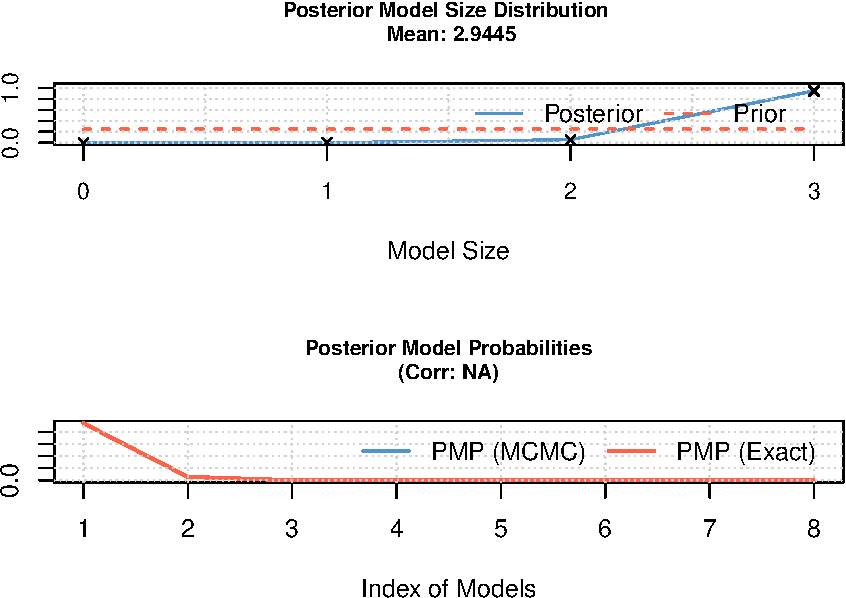
\includegraphics{02-probability_and_distribution_files/figure-latex/unnamed-chunk-37-1} 

}

\caption{伽马分布:不同参数组合下的概率密度函数}\label{fig:unnamed-chunk-37}
\end{figure}

\hypertarget{ux8d1dux5854ux5206ux5e03ux6bd4ux4f8bux53d8ux91cfux7684ux5929ux7136ux9009ux62e9}{%
\subsection{贝塔分布:比例变量的天然选择}\label{ux8d1dux5854ux5206ux5e03ux6bd4ux4f8bux53d8ux91cfux7684ux5929ux7136ux9009ux62e9}}

\textbf{故事引入:} 在蚱蜢的日常生活中,时间分配是一个重要的生态学问题。这只蚱蜢在一天24小时中,用于觅食(午餐和其他进食)的时间比例是多少?可能是30\%,也可能是60\%,这个比例值总是在0和1之间。贝塔分布是描述这类比例变量的理想选择,它能够灵活地刻画蚱蜢在不同环境条件下时间分配模式的多样性。

\textbf{数学定义:} 贝塔分布的概率密度函数为:

\[f(x) = \frac{x^{\alpha-1}(1-x)^{\beta-1}}{B(\alpha, \beta)}, \quad 0 \leq x \leq 1\]

其中\(\alpha > 0\)和\(\beta > 0\)是形状参数,\(B(\alpha, \beta)\)是贝塔函数。

\textbf{分布特性:}
- 期望值:\(E[X] = \frac{\alpha}{\alpha + \beta}\)
- 方差:\(Var(X) = \frac{\alpha\beta}{(\alpha+\beta)^2(\alpha+\beta+1)}\)
- 分布形状极其灵活,可以呈现U形、J形、钟形等多种形态
- 当\(\alpha = \beta = 1\)时,贝塔分布退化为均匀分布
- 贝塔分布是二项分布和伯努利分布的共轭先验

\textbf{生态学肖像:}

贝塔分布在生态学中具有广泛的应用价值,特别适合描述比例变量的分布特征。在行为生态学中,贝塔分布能够精确刻画蚱蜢一天中用于觅食、休息、警戒等不同行为的时间比例分配模式。这种分布同样适用于建模蚱蜢对不同植物种类的资源选择偏好,通过比例值反映其选择倾向的强度。在能量预算分析方面,贝塔分布帮助研究者通过时间分配比例来深入探讨蚱蜢的能量摄入与消耗平衡机制。贝塔分布的灵活性使其特别适合描述动物在不同环境条件下的适应性行为调整,能够捕捉行为模式随环境变化的动态特征。

\begin{figure}

{\centering 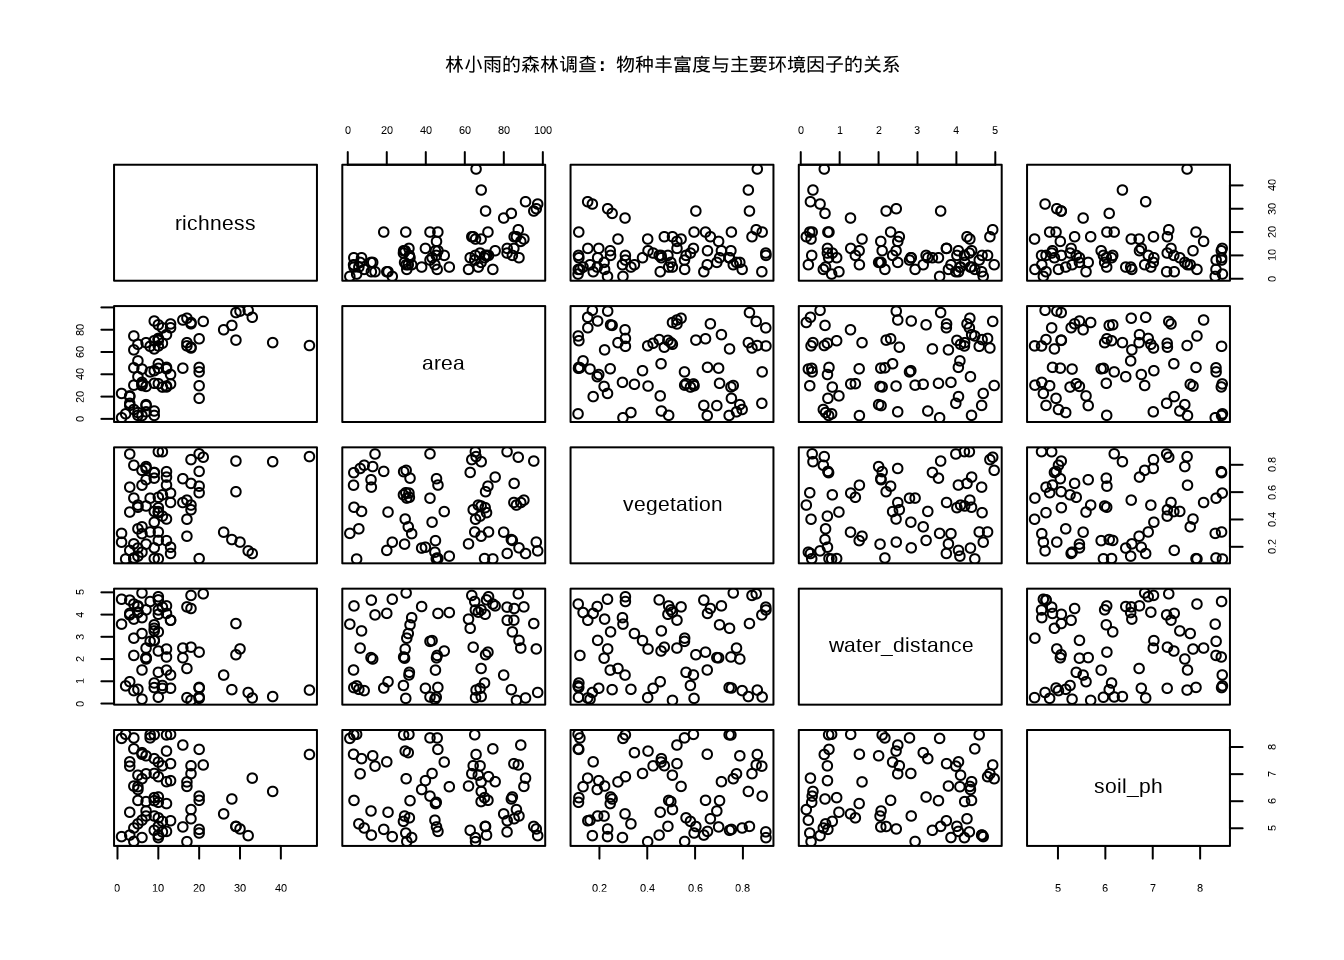
\includegraphics{02-probability_and_distribution_files/figure-latex/unnamed-chunk-38-1} 

}

\caption{贝塔分布:不同参数组合下的概率密度函数}\label{fig:unnamed-chunk-38}
\end{figure}

\hypertarget{ux6b63ux6001ux7684ux9b54ux529bux4e2dux5fc3ux6781ux9650ux5b9aux7406}{%
\subsection{正态的魔力:中心极限定理}\label{ux6b63ux6001ux7684ux9b54ux529bux4e2dux5fc3ux6781ux9650ux5b9aux7406}}

在我们探索蚱蜢午餐行为的过程中,正态分布以其优雅的钟形曲线给我们留下了深刻印象。但正态分布的真正魔力远不止于此------它拥有一个被称为''统计学的魔法石''的非凡性质:\textbf{中心极限定理}。这个定理解释了为什么正态分布在自然界和统计学中无处不在,即使原始数据本身并不服从正态分布。

\hypertarget{ux4ec0ux4e48ux662fux4e2dux5fc3ux6781ux9650ux5b9aux7406}{%
\subsubsection{什么是中心极限定理}\label{ux4ec0ux4e48ux662fux4e2dux5fc3ux6781ux9650ux5b9aux7406}}

\textbf{中心极限定理}(Central Limit Theorem, CLT)是概率论和统计学中最重要的定理之一。它的核心思想可以概括为:

\begin{quote}
无论原始总体的分布形态如何,只要样本量足够大,样本均值的抽样分布就会近似服从正态分布。
\end{quote}

更精确地说,中心极限定理指出:
- 从任意分布(无论是什么形状)的总体中随机抽取样本
- 计算每个样本的均值
- 当样本量\(n\)足够大时(通常\(n \geq 30\)),这些样本均值的分布将近似正态分布
- 这个正态分布的均值等于总体均值\(\mu\),标准差等于总体标准差\(\sigma\)除以\(\sqrt{n}\)

\textbf{数学表达:}
如果\(X_1, X_2, \ldots, X_n\)是来自均值为\(\mu\)、方差为\(\sigma^2\)的总体的独立同分布随机变量,那么当\(n \to \infty\)时:

\[\frac{\bar{X} - \mu}{\sigma/\sqrt{n}} \xrightarrow{d} N(0, 1)\]

其中\(\bar{X} = \frac{1}{n}\sum_{i=1}^n X_i\)是样本均值,\(\xrightarrow{d}\)表示依分布收敛。

\begin{figure}

{\centering 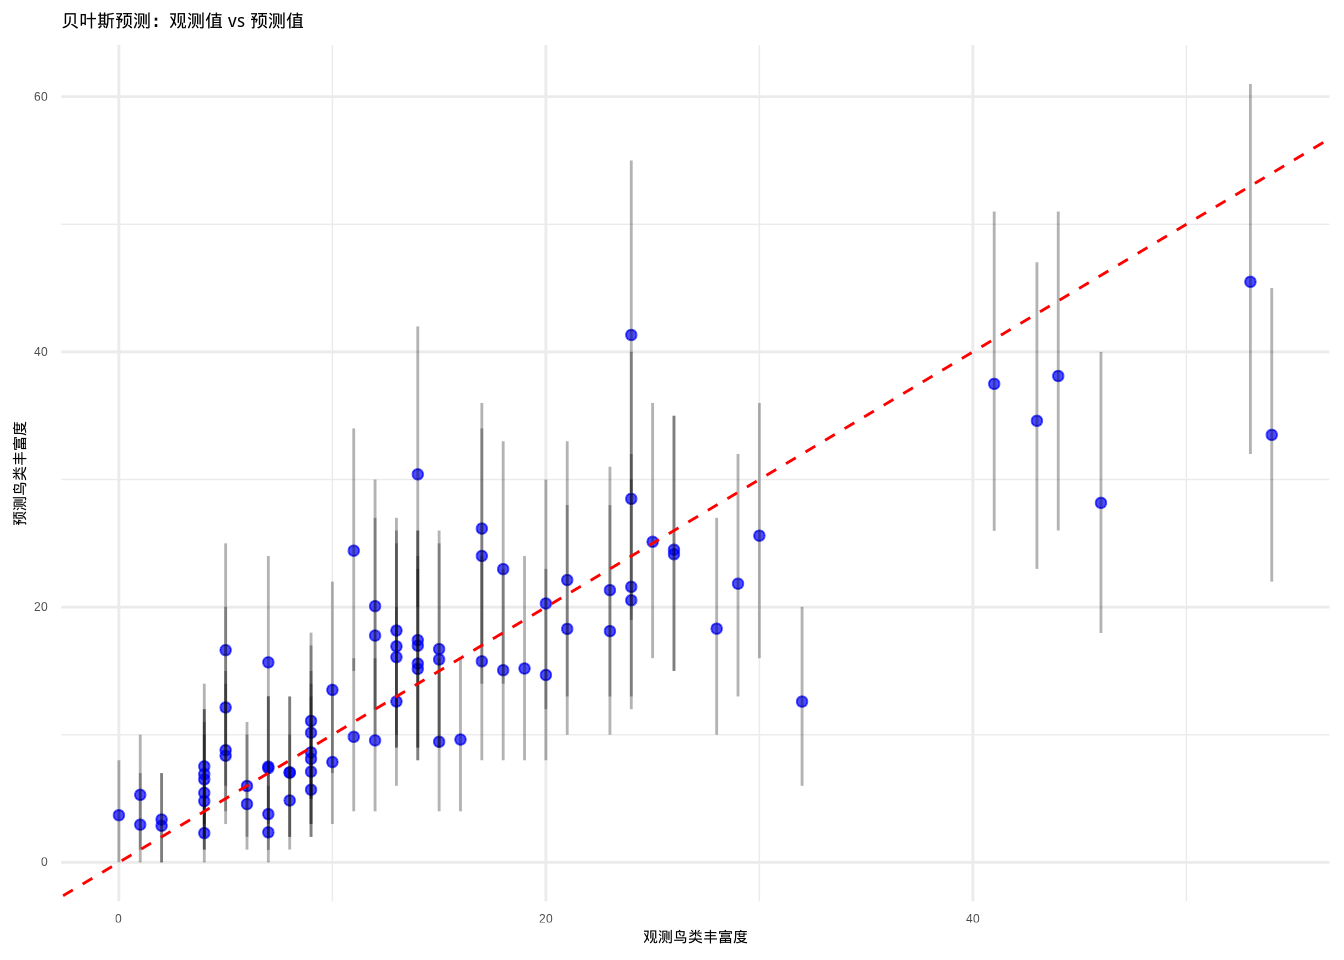
\includegraphics{02-probability_and_distribution_files/figure-latex/unnamed-chunk-39-1} 

}

\caption{中心极限定理演示:不同总体分布下样本均值的正态收敛过程}\label{fig:unnamed-chunk-39}
\end{figure}

\begin{verbatim}
## 中心极限定理正态性检验结果:
\end{verbatim}

\begin{verbatim}
## 均匀分布样本均值Kolmogorov-Smirnov p值: 0.9917
\end{verbatim}

\begin{verbatim}
## 指数分布样本均值Kolmogorov-Smirnov p值: 0
\end{verbatim}

\begin{verbatim}
## 伽马分布样本均值Kolmogorov-Smirnov p值: 0.0014
\end{verbatim}

\begin{verbatim}
## 贝塔分布样本均值Kolmogorov-Smirnov p值: 0.0179
\end{verbatim}

\hypertarget{ux6837ux672cux91cfux5bf9ux4e2dux5fc3ux6781ux9650ux5b9aux7406ux7684ux5f71ux54cd}{%
\subsubsection{样本量对中心极限定理的影响}\label{ux6837ux672cux91cfux5bf9ux4e2dux5fc3ux6781ux9650ux5b9aux7406ux7684ux5f71ux54cd}}

\begin{figure}

{\centering 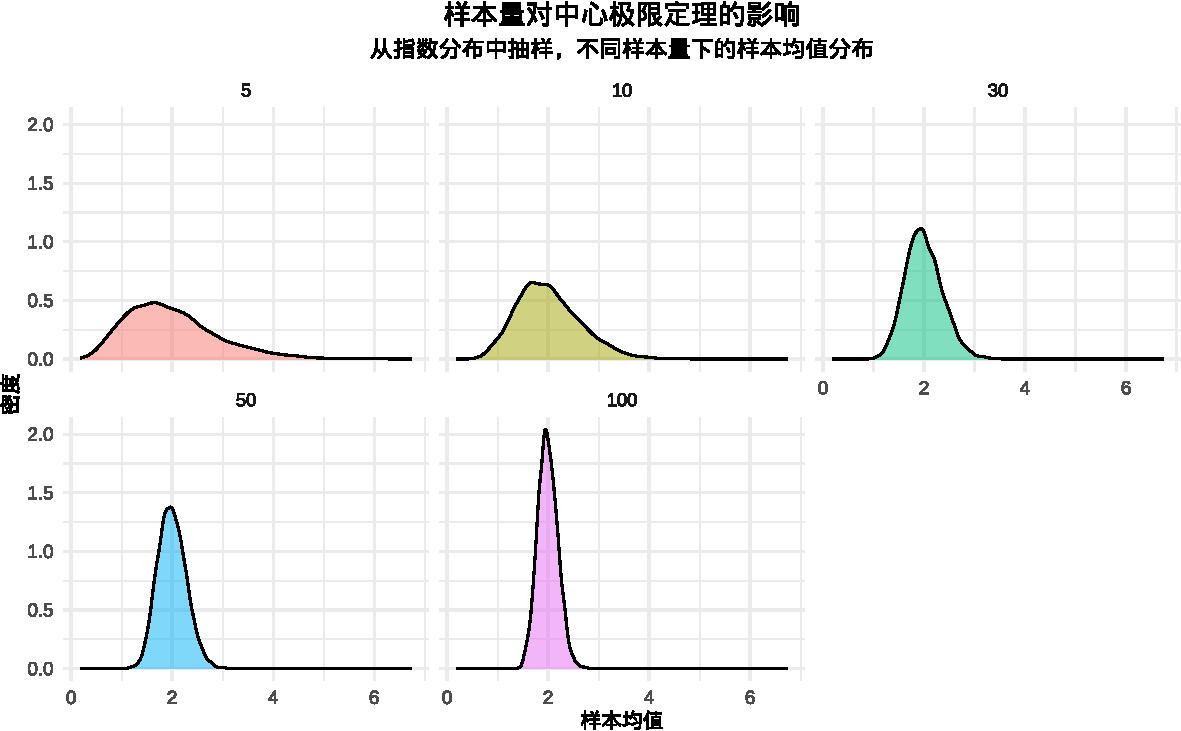
\includegraphics{02-probability_and_distribution_files/figure-latex/unnamed-chunk-40-1} 

}

\caption{样本量对中心极限定理的影响:样本量越大,样本均值分布越接近正态}\label{fig:unnamed-chunk-40}
\end{figure}

\begin{verbatim}
## 偏度和峰度随样本量的变化:
\end{verbatim}

\begin{verbatim}
##   SampleSize  Skewness Kurtosis
## 1          5 0.8974114 4.109759
## 2         10 0.6504552 3.732605
## 3         30 0.4054190 3.315501
## 4         50 0.2691500 3.072610
## 5        100 0.2423726 3.087874
\end{verbatim}

\hypertarget{ux86b1ux8722ux5348ux9910ux4e2dux7684ux4e2dux5fc3ux6781ux9650ux5b9aux7406}{%
\subsubsection{蚱蜢午餐中的中心极限定理}\label{ux86b1ux8722ux5348ux9910ux4e2dux7684ux4e2dux5fc3ux6781ux9650ux5b9aux7406}}

在蚱蜢的生态研究中,中心极限定理展现出其强大的应用价值。虽然单个蚱蜢的摄食量可能呈现偏斜分布,但当我们随机抽取30只蚱蜢并计算其平均摄食量,多次重复这一抽样过程后,样本均值的分布将呈现完美的钟形曲线。同样,蚱蜢的觅食时间虽受多种因素影响而分布不规则,但通过中心极限定理,我们能够基于样本均值可靠地估计整个种群的
平均觅食时间。即使蚱蜢对植物的选择偏好本身不是正态分布,当我们研究多个样本的平均偏好时,结果也会趋于正态分布。这些生态学场景生动地展示了中心极限定理如何将复杂的个体变异转化为可预测的统计规律,为生态学研究提供了坚实的理论基础。

\hypertarget{ux4e2dux5fc3ux6781ux9650ux5b9aux7406ux7684ux751fux6001ux5b66ux610fux4e49}{%
\subsubsection{中心极限定理的生态学意义}\label{ux4e2dux5fc3ux6781ux9650ux5b9aux7406ux7684ux751fux6001ux5b66ux610fux4e49}}

中心极限定理为生态学研究提供了坚实的理论支撑,确保了统计推断的可靠性。即使我们不知道总体的真实分布,通过样本均值来估计总体参数时,这种估计的误差分布是正态的,这为参数估计提供了数学保障。许多常用的统计检验方法,如t检验和方差分析,都建立在中心极限定理的基础上,假设样本均值的分布是正态的。基于这一定理,我们能够构建总体均值的置信区间,为生态学推断提供量化依据。更重要的是,中心极限定理构成了大样本统计方法的理论基石,使得在样本量足够大的情况下,我们能够做出可靠的统计推断,为生态学的定量研究奠定了坚实的数学基础。

\hypertarget{ux4e2dux5fc3ux6781ux9650ux5b9aux7406ux7684ux5c40ux9650ux6027}{%
\subsubsection{中心极限定理的局限性}\label{ux4e2dux5fc3ux6781ux9650ux5b9aux7406ux7684ux5c40ux9650ux6027}}

尽管中心极限定理非常强大,但在应用时也需要注意其局限性。该定理要求样本量足够大(通常\(n \geq 30\)),对于小样本情况,正态近似的效果可能不佳。样本必须是独立同分布的,如果存在空间自相关或时间序列依赖,定理可能不适用。总体方差必须是有限的,对于方差无限的重尾分布,中心极限定理可能不成立。此外,不同分布的收敛速度存在差异,有些分布需要更大的样本量才能达到较好的正态近似效果。这些局限性提醒我们在应用中心极限定理时需要谨慎考虑其适用条件。

\hypertarget{ux751fux6001ux5b66ux5e94ux7528ux5b9eux4f8b}{%
\subsection{生态学应用实例}\label{ux751fux6001ux5b66ux5e94ux7528ux5b9eux4f8b}}

\textbf{种群密度估计}
通过在不同样方中计数物种个体数,即使个体分布本身是聚集的(如负二项分布),样本均值的分布仍近似正态,这使得我们能够可靠地估计总体密度。

\textbf{环境梯度研究}
沿着环境梯度(如海拔、温度)测量物种丰富度,即使原始数据呈现复杂模式,样本均值的分布仍趋于正态,便于统计分析和建模。

\textbf{行为生态学实验}
在控制实验中测量动物的行为参数,通过中心极限定理,我们可以基于样本均值进行可靠的统计推断。

\hypertarget{ux603bux7ed3-1}{%
\subsubsection{总结}\label{ux603bux7ed3-1}}

中心极限定理是连接概率论与统计推断的桥梁,它解释了为什么正态分布在统计学中占据核心地位。在蚱蜢午餐的研究中,这个定理确保了即使面对复杂的生态数据,我们仍然能够使用基于正态分布的统计方法来获得可靠的科学结论。

正如统计学家乔治·博克斯所言:``所有的模型都是错的,但有些是有用的。''中心极限定理正是这样一个''有用''的模型,它虽然不是绝对精确,但在大多数实际情况下提供了足够好的近似,为生态学的定量研究奠定了坚实的数学基础。

\hypertarget{ux6df7ux5408ux5206ux5e03ux5904ux7406ux5f02ux8d28ux6027ux6570ux636e}{%
\section{混合分布:处理异质性数据}\label{ux6df7ux5408ux5206ux5e03ux5904ux7406ux5f02ux8d28ux6027ux6570ux636e}}

混合分布能够描述来自不同子总体的数据,在生态学中处理异质性非常有用。

\begin{figure}

{\centering 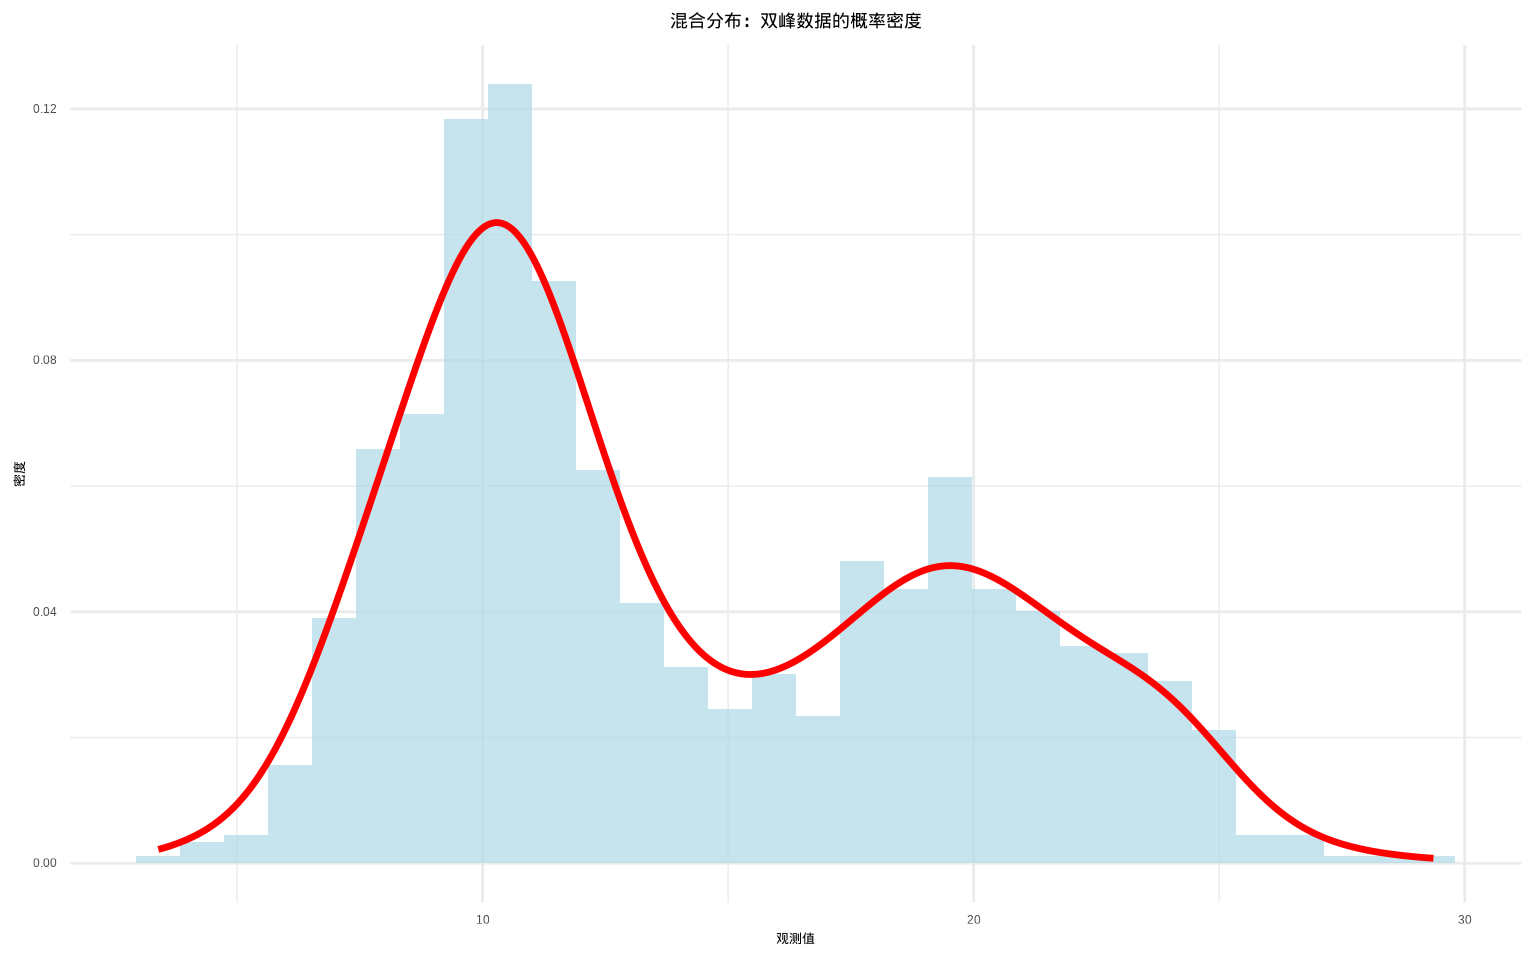
\includegraphics{02-probability_and_distribution_files/figure-latex/unnamed-chunk-41-1} 

}

\caption{混合分布:双峰数据的概率密度函数}\label{fig:unnamed-chunk-41}
\end{figure}

\begin{verbatim}
## 混合分布的生态学应用:
\end{verbatim}

\begin{verbatim}
## 1. 不同年龄组的种群结构
\end{verbatim}

\begin{verbatim}
## 2. 异质环境中的物种分布
\end{verbatim}

\begin{verbatim}
## 3. 多物种混合的群落数据
\end{verbatim}

\begin{verbatim}
## 4. 季节性变化的环境因子
\end{verbatim}

\hypertarget{ux96f6ux81a8ux80c0ux5206ux5e03ux5904ux7406ux96f6ux503cux8fc7ux591aux7684ux6570ux636e}{%
\subsection{零膨胀分布:处理零值过多的数据}\label{ux96f6ux81a8ux80c0ux5206ux5e03ux5904ux7406ux96f6ux503cux8fc7ux591aux7684ux6570ux636e}}

在生态学中,许多计数数据存在大量的零值,零膨胀分布专门处理这类数据。

\begin{Shaded}
\begin{Highlighting}[]
\CommentTok{\# 零膨胀分布概念演示}
\FunctionTok{set.seed}\NormalTok{(}\DecValTok{2323}\NormalTok{)}

\CommentTok{\# 模拟零膨胀数据:80\%的零值和20\%的泊松分布}
\NormalTok{n\_samples }\OtherTok{\textless{}{-}} \DecValTok{1000}
\NormalTok{zero\_prob }\OtherTok{\textless{}{-}} \FloatTok{0.8}
\NormalTok{lambda }\OtherTok{\textless{}{-}} \DecValTok{3}

\CommentTok{\# 生成零膨胀泊松数据}
\NormalTok{zip\_data }\OtherTok{\textless{}{-}} \FunctionTok{numeric}\NormalTok{(n\_samples)}
\ControlFlowTok{for}\NormalTok{ (i }\ControlFlowTok{in} \DecValTok{1}\SpecialCharTok{:}\NormalTok{n\_samples) \{}
  \ControlFlowTok{if}\NormalTok{ (}\FunctionTok{runif}\NormalTok{(}\DecValTok{1}\NormalTok{) }\SpecialCharTok{\textless{}}\NormalTok{ zero\_prob) \{}
\NormalTok{    zip\_data[i] }\OtherTok{\textless{}{-}} \DecValTok{0}
\NormalTok{  \} }\ControlFlowTok{else}\NormalTok{ \{}
\NormalTok{    zip\_data[i] }\OtherTok{\textless{}{-}} \FunctionTok{rpois}\NormalTok{(}\DecValTok{1}\NormalTok{, lambda)}
\NormalTok{  \}}
\NormalTok{\}}

\CommentTok{\# 统计零值比例}
\NormalTok{zero\_proportion }\OtherTok{\textless{}{-}} \FunctionTok{mean}\NormalTok{(zip\_data }\SpecialCharTok{==} \DecValTok{0}\NormalTok{)}
\FunctionTok{cat}\NormalTok{(}\StringTok{"零膨胀数据统计:}\SpecialCharTok{\textbackslash{}n}\StringTok{"}\NormalTok{,}
  \StringTok{"零值比例:"}\NormalTok{, }\FunctionTok{round}\NormalTok{(zero\_proportion, }\DecValTok{3}\NormalTok{), }\StringTok{"}\SpecialCharTok{\textbackslash{}n}\StringTok{"}\NormalTok{,}
  \StringTok{"非零值均值:"}\NormalTok{, }\FunctionTok{round}\NormalTok{(}\FunctionTok{mean}\NormalTok{(zip\_data[zip\_data }\SpecialCharTok{\textgreater{}} \DecValTok{0}\NormalTok{]), }\DecValTok{3}\NormalTok{), }\StringTok{"}\SpecialCharTok{\textbackslash{}n}\StringTok{"}\NormalTok{,}
  \StringTok{"总体均值:"}\NormalTok{, }\FunctionTok{round}\NormalTok{(}\FunctionTok{mean}\NormalTok{(zip\_data), }\DecValTok{3}\NormalTok{), }\StringTok{"}\SpecialCharTok{\textbackslash{}n}\StringTok{"}\NormalTok{)}
\end{Highlighting}
\end{Shaded}

\begin{verbatim}
## 零膨胀数据统计:
##  零值比例: 0.793 
##  非零值均值: 3.266 
##  总体均值: 0.676
\end{verbatim}

\begin{Shaded}
\begin{Highlighting}[]
\CommentTok{\# 与普通泊松分布比较}
\NormalTok{poisson\_data }\OtherTok{\textless{}{-}} \FunctionTok{rpois}\NormalTok{(n\_samples, }\AttributeTok{lambda =} \FunctionTok{mean}\NormalTok{(zip\_data))}
\FunctionTok{cat}\NormalTok{(}\StringTok{"}\SpecialCharTok{\textbackslash{}n}\StringTok{与普通泊松分布比较:}\SpecialCharTok{\textbackslash{}n}\StringTok{"}\NormalTok{,}
  \StringTok{"泊松零值比例:"}\NormalTok{, }\FunctionTok{round}\NormalTok{(}\FunctionTok{mean}\NormalTok{(poisson\_data }\SpecialCharTok{==} \DecValTok{0}\NormalTok{), }\DecValTok{3}\NormalTok{), }\StringTok{"}\SpecialCharTok{\textbackslash{}n}\StringTok{"}\NormalTok{,}
  \StringTok{"泊松方差:"}\NormalTok{, }\FunctionTok{round}\NormalTok{(}\FunctionTok{var}\NormalTok{(poisson\_data), }\DecValTok{3}\NormalTok{), }\StringTok{"}\SpecialCharTok{\textbackslash{}n}\StringTok{"}\NormalTok{,}
  \StringTok{"零膨胀方差:"}\NormalTok{, }\FunctionTok{round}\NormalTok{(}\FunctionTok{var}\NormalTok{(zip\_data), }\DecValTok{3}\NormalTok{), }\StringTok{"}\SpecialCharTok{\textbackslash{}n}\StringTok{"}\NormalTok{,}
  \StringTok{"过度分散指数:"}\NormalTok{, }\FunctionTok{round}\NormalTok{(}\FunctionTok{var}\NormalTok{(zip\_data) }\SpecialCharTok{/} \FunctionTok{mean}\NormalTok{(zip\_data), }\DecValTok{3}\NormalTok{), }\StringTok{"}\SpecialCharTok{\textbackslash{}n}\StringTok{"}\NormalTok{)}
\end{Highlighting}
\end{Shaded}

\begin{verbatim}
## 
## 与普通泊松分布比较:
##  泊松零值比例: 0.534 
##  泊松方差: 0.657 
##  零膨胀方差: 2.361 
##  过度分散指数: 3.493
\end{verbatim}

\begin{Shaded}
\begin{Highlighting}[]
\CommentTok{\# 零膨胀分布的生态学意义}
\FunctionTok{cat}\NormalTok{(}\StringTok{"}\SpecialCharTok{\textbackslash{}n}\StringTok{零膨胀分布的生态学应用:}\SpecialCharTok{\textbackslash{}n}\StringTok{"}\NormalTok{)}
\end{Highlighting}
\end{Shaded}

\begin{verbatim}
## 
## 零膨胀分布的生态学应用:
\end{verbatim}

\begin{Shaded}
\begin{Highlighting}[]
\FunctionTok{cat}\NormalTok{(}\StringTok{"1. 稀有物种的出现数据}\SpecialCharTok{\textbackslash{}n}\StringTok{"}\NormalTok{)}
\end{Highlighting}
\end{Shaded}

\begin{verbatim}
## 1. 稀有物种的出现数据
\end{verbatim}

\begin{Shaded}
\begin{Highlighting}[]
\FunctionTok{cat}\NormalTok{(}\StringTok{"2. 低密度种群的分布数据}\SpecialCharTok{\textbackslash{}n}\StringTok{"}\NormalTok{)}
\end{Highlighting}
\end{Shaded}

\begin{verbatim}
## 2. 低密度种群的分布数据
\end{verbatim}

\begin{Shaded}
\begin{Highlighting}[]
\FunctionTok{cat}\NormalTok{(}\StringTok{"3. 间歇性生态过程记录}\SpecialCharTok{\textbackslash{}n}\StringTok{"}\NormalTok{)}
\end{Highlighting}
\end{Shaded}

\begin{verbatim}
## 3. 间歇性生态过程记录
\end{verbatim}

\begin{Shaded}
\begin{Highlighting}[]
\FunctionTok{cat}\NormalTok{(}\StringTok{"4. 不完全调查的观测数据}\SpecialCharTok{\textbackslash{}n}\StringTok{"}\NormalTok{)}
\end{Highlighting}
\end{Shaded}

\begin{verbatim}
## 4. 不完全调查的观测数据
\end{verbatim}

零膨胀分布在生态学中具有重要的应用价值,专门用于处理存在大量零值的计数数据。这种分布在以下生态学场景中特别有用:

\begin{enumerate}
\def\labelenumi{\arabic{enumi}.}
\item
  \textbf{稀有物种的出现数据}:在生态调查中,许多稀有物种在大多数样方中不出现,导致数据中存在大量零值。零膨胀分布能够准确描述这种零值过多的模式。
\item
  \textbf{低密度种群的分布数据}:当种群密度很低时,即使物种存在,也可能在大多数调查点无法观测到,形成零值聚集的数据结构。
\item
  \textbf{间歇性生态过程记录}:某些生态过程(如动物活动、植物开花等)具有间歇性特征,在时间序列中产生大量零值观测。
\item
  \textbf{不完全调查的观测数据}:由于调查方法限制或环境条件影响,某些生态调查可能无法完全覆盖目标区域,导致观测数据中存在系统性的零值。
\end{enumerate}

\hypertarget{ux603bux7ed3-2}{%
\section{总结}\label{ux603bux7ed3-2}}

本章系统性地构建了生态学研究中理解不确定性的数学框架,从基础的概率概念到复杂的分布理论,为生态学家提供了量化自然世界随机性的强大工具。通过蚱蜢午餐选择的生动案例,我们逐步揭示了概率理论在生态学中的深刻意义和应用价值。

概率理论为我们提供了三种理解不确定性的不同视角。古典概率基于等可能性假设,为我们提供了理想化的理论基准,虽然其假设在现实生态系统中往往过于简化,但作为思维起点具有重要价值。频率概率通过实际观察数据来量化生态现象,体现了经验主义的研究方法,其核心的大数定律确保了长期观察的稳定性。贝叶斯概率则引入了动态更新的思想,能够结合先验知识和新证据,更接近生态学家实际的认知过程,特别适合处理数据有限但专家知识丰富的生态问题。

随机变量的概念将生态现象转化为数学语言,使我们能够精确描述生物行为和环境变化的不确定性。离散随机变量处理可数的生态事件,如物种选择、行为决策等,而连续随机变量则描述测量值的变化,如生物体尺寸、环境因子等。概率分布作为随机变量的数学指纹,完整刻画了生态现象的统计规律。

在离散分布家族中,伯努利分布描述了二元选择的基本模式,是构建更复杂模型的基础。二项分布将单次试验扩展到多次重复,适用于种群估计、繁殖成功率等计数问题。多项式分布处理多元选择场景,能够描述群落组成、资源分配等复杂生态系统的联合概率分布。泊松分布专门处理稀有事件和空间分布问题,是研究稀有物种分布和随机分布模式的重要工具。几何分布和负二项分布则关注等待时间问题,分别描述第一次成功和第r次成功所需的努力,在行为生态学和进化研究中具有重要应用。

连续分布家族则为我们提供了描述测量值变化的数学工具。均匀分布刻画了完全随机的选择过程,指数分布描述了事件发生的时间间隔,特别适合生存分析和风险建模。正态分布以其经典的钟形曲线和中心极限定理的支撑,成为生态学中最常用的分布之一,能够描述大多数受到多重微小因素影响的生态变量。威布尔分布提供了更灵活的生存分析工具,能够刻画随时间变化的死亡风险模式。伽马分布作为指数分布的一般化,适用于描述累积等待时间和生物量积累过程。贝塔分布则是处理比例变量的理想选择,特别适合行为时间分配和资源选择偏好的研究。

中心极限定理作为概率论的核心成果,解释了为什么正态分布在统计学中如此普遍。无论原始总体分布形态如何,只要样本量足够大,样本均值的分布就会趋于正态,这为生态学的统计推断提供了坚实的理论基础。通过这个定理,我们能够在不知道总体真实分布的情况下,仍然能够进行可靠的参数估计和假设检验。

在生态学实践中,我们还需要处理更复杂的数据结构。混合分布能够描述来自不同子总体的异质性数据,如不同年龄组的种群结构或异质环境中的物种分布。零膨胀分布专门处理存在大量零值的计数数据,这在稀有物种研究和低密度种群监测中尤为重要。

概率与分布理论的价值不仅在于提供具体的计算方法,更在于培养一种''概率思维''------用数学语言理解和描述生态世界的能力。在人工智能技术快速发展的今天,这种能力显得尤为重要。AI模型虽然能够处理海量数据,但其输出本质上是概率性的,只有深刻理解概率原理,才能正确解读AI的预测结果,评估模型的可信度。

生态学研究面对的是自然界中最为复杂的系统之一,与物理实验不同,生态学观察往往无法在完全控制的条件下重复进行。概率与分布理论为我们提供了量化这种不确定性的语言,帮助我们设计合理的生态调查方案,正确解读复杂的生态数据,与数据科学家有效合作,并在AI时代保持批判性和创造性。

通过本章的学习,我们不仅掌握了概率与分布的基本概念和计算方法,更重要的是建立了连接生态观察与数学分析的桥梁。这种数学框架使我们能够从定性的生态描述迈向定量的科学分析,为理解生物决策机制、种群动态、群落结构等生态学核心问题提供了强有力的工具。在数据驱动的生态学时代,概率与分布理论将继续发挥不可替代的作用,帮助我们更好地理解和保护这个充满不确定性的自然世界。

\hypertarget{ux63cfux8ff0ux7edfux8ba1}{%
\chapter{描述统计}\label{ux63cfux8ff0ux7edfux8ba1}}

\hypertarget{ux5f15ux8a00-2}{%
\section{引言}\label{ux5f15ux8a00-2}}

上一章我们探索了概率分布的奥秘,认识到要完整刻画一个随机变量的特征,最理想的方式是掌握其概率分布的全貌。然而在生态学研究的现实世界中,获取完整的概率分布信息往往如同捕捉风中的细沙------既困难又充满挑战。想象一下,我们要描绘一片原始森林中所有树木的高度分布,或是记录一个深邃湖泊中所有鱼类的体重分布,我们不可能逐一测量每一个生命个体。在这种现实约束下,描述统计便成为了我们解读生态系统密码的钥匙。

描述统计宛如生态学家的''数字望远镜''和''统计显微镜'',它赋予我们穿透复杂生态现象迷雾的能力,从纷繁的自然数据中提炼出关键特征,用精炼的数值语言来概括和描述我们观察到的生态模式。这些统计特征不仅是理解当前生态状况的窗口,更是我们进行科学比较、趋势预测和管理决策的基石。

让我们从一幅生动的生态画卷开始思考。假设你是一名野生动物保护工作者,正守护着一片保护区内的梅花鹿种群。你无法追踪每一只梅花鹿的足迹,但通过科学的抽样调查,你测量了50只梅花鹿的体重。这些体重数据如同散落的珍珠,呈现出怎样的分布特征呢?有些梅花鹿体态轻盈,体重约30公斤;有些则身姿矫健,体重可达60公斤以上;而大多数梅花鹿的体重则集中在40-50公斤之间。描述统计就是将这些观察转化为科学语言的魔法------均值揭示种群的平均体重水平,标准差展现个体间的体重差异程度,偏度描绘体重分布的对称性,峰度则暗示极端体重个体的出现频率。

再让我们潜入一个更为复杂的生态场景。你正研究一片湿地生态系统中不同水鸟物种的多样性。你无法记录每一只水鸟的每一次翩跹,但通过系统的定期调查,你获得了各个物种的观测频率。描述统计中的多样性指数(如Shannon-Wiener指数、Simpson指数)便将这些频率数据转化为对群落复杂性的量化描述。这些指数不仅告诉你这片湿地栖息着多少种水鸟,更重要的是揭示了物种相对多度分布的均衡性------是少数优势物种主导的寡头格局,还是各个物种相对均匀分布的民主格局?这种信息对于评估生态系统的健康状况和制定精准的保护策略具有决定性意义。

描述统计在生态学中的应用如同繁星点点,遍布各个研究领域。当你探究气候变化对植物物候的影响时,你需要描述开花时间的年际波动;当你分析污染物在食物链中的富集过程时,你需要刻画不同营养级生物体内污染物的浓度分布;当你评估生态恢复项目的成效时,你需要量化恢复前后关键生态指标的变化轨迹。在这些多元情境下,描述统计提供的中心趋势、离散程度和分布形状等特征,构成了我们理解和沟通生态现象的共同语言。

更为重要的是,描述统计架起了观察数据与理论模型之间的桥梁。生态学理论往往预言特定的统计模式------竞争排斥理论预测物种多度分布应呈现特定的形态;岛屿生物地理学理论预示物种-面积关系应遵循幂律分布;生态位理论推演个体大小分布应符合特定的统计规律。通过描述统计,我们能够检验这些理论预言是否与观察数据相契合,从而推动生态学理论的演进与完善。

让我们深入思考一个具体的生态学谜题:为什么有些湖泊的鱼类群落比另一些更加稳定?描述统计为我们提供了破解这一谜题的钥匙。通过计算各个湖泊鱼类群落的多样性指数、均匀度指数,以及分析物种多度分布的形状特征,我们可能发现稳定性较高的群落往往具有更高的物种多样性、更均匀的物种多度分布,以及特定的多度分布模式。这些统计特征不仅描绘了群落的现状图景,更重要的是揭示了维持群落稳定性的深层机制。

在环境监测和生态风险评估的战场上,描述统计同样扮演着关键角色。想象你肩负着监测一条河流水质变化的使命。你定期测量水中的各种污染物浓度、pH值、溶解氧等关键指标。描述统计让你能够量化这些指标的正常波动范围(通过均值和标准差),识别异常值(通过极值和异常值检测),以及刻画长期变化趋势(通过时间序列分析)。当某个指标超出正常范围时,这些统计特征如同预警系统的哨兵,帮助你及时采取干预措施,守护生态安全。

对于生态学专业的学生而言,掌握描述统计不仅是完成学业的要求,更是培养科学思维方式的必经之路。生态学研究的对象往往是复杂、多变、充满不确定性的自然系统。描述统计教会我们如何在不确定性中寻找确定性,在复杂性中发现简单性,在变化中识别规律性。这种能力不仅对生态学研究至关重要,对任何需要处理复杂数据的领域都具有深远价值。

最后,让我们思考描述统计在生态学教育中的深层意义。当你学习描述统计时,你不仅仅是在掌握数学公式和计算方法,你是在学习如何用科学的语言描述自然界的韵律。均值、方差、偏度、峰度这些概念,都是生态学家用来理解和交流生态现象的工具箱。掌握这些工具,意味着你能够更准确地观察自然的脉动、更深刻地理解生态过程的机理、更有效地沟通科学发现的精髓。

在接下来的章节中,我们将系统地探索各种描述统计方法,从最基础的中心趋势测量到复杂的分布形状描述,从个体特征到群落结构,从空间异质性到时间动态。每一个统计量都有其独特的生态学意义和应用场景。通过学习这些方法,你将能够将原始的生态数据转化为有意义的科学信息,为你的生态学研究奠定坚实的统计基础。

\hypertarget{ux63cfux8ff0ux7edfux8ba1ux57faux7840}{%
\section{描述统计基础}\label{ux63cfux8ff0ux7edfux8ba1ux57faux7840}}

\hypertarget{ux4e2dux5fc3ux8d8bux52bfux6d4bux91cf}{%
\subsection{中心趋势测量}\label{ux4e2dux5fc3ux8d8bux52bfux6d4bux91cf}}

中心趋势测量帮助我们定位数据的''引力中心'',如同探寻一片森林中最具代表性的树木高度,或是识别一个湖泊中最典型的鱼类大小。这些统计量为我们提供了理解生态数据分布格局的关键锚点。

\textbf{均值}:

\textbf{数学定义}:对于一组观测值 \(x_1, x_2, \ldots, x_n\),算术平均定义为:

\[\bar{x} = \frac{1}{n}\sum_{i=1}^{n}x_i\]

几何平均定义为:

\[G = \left(\prod_{i=1}^{n}x_i\right)^{\frac{1}{n}}\]

调和平均定义为:

\[H = \frac{n}{\sum_{i=1}^{n}\frac{1}{x_i}}\]

想象你正在研究一片温带森林中红松的胸径分布。你随机测量了100棵红松的胸径(单位:厘米),得到了以下数据:

\begin{Shaded}
\begin{Highlighting}[]
\CommentTok{\# 模拟红松胸径数据 {-} 创建40棵红松的胸径观测值}
\CommentTok{\# 这些数据模拟了森林中红松种群的实际胸径分布}
\NormalTok{pine\_diameter }\OtherTok{\textless{}{-}} \FunctionTok{c}\NormalTok{(}
  \DecValTok{25}\NormalTok{, }\DecValTok{28}\NormalTok{, }\DecValTok{32}\NormalTok{, }\DecValTok{35}\NormalTok{, }\DecValTok{38}\NormalTok{, }\DecValTok{40}\NormalTok{, }\DecValTok{42}\NormalTok{, }\DecValTok{45}\NormalTok{, }\DecValTok{48}\NormalTok{, }\DecValTok{50}\NormalTok{,}
  \DecValTok{52}\NormalTok{, }\DecValTok{55}\NormalTok{, }\DecValTok{58}\NormalTok{, }\DecValTok{60}\NormalTok{, }\DecValTok{62}\NormalTok{, }\DecValTok{65}\NormalTok{, }\DecValTok{68}\NormalTok{, }\DecValTok{70}\NormalTok{, }\DecValTok{72}\NormalTok{, }\DecValTok{75}\NormalTok{,}
  \DecValTok{30}\NormalTok{, }\DecValTok{33}\NormalTok{, }\DecValTok{36}\NormalTok{, }\DecValTok{39}\NormalTok{, }\DecValTok{41}\NormalTok{, }\DecValTok{43}\NormalTok{, }\DecValTok{46}\NormalTok{, }\DecValTok{49}\NormalTok{, }\DecValTok{51}\NormalTok{, }\DecValTok{53}\NormalTok{,}
  \DecValTok{56}\NormalTok{, }\DecValTok{59}\NormalTok{, }\DecValTok{61}\NormalTok{, }\DecValTok{63}\NormalTok{, }\DecValTok{66}\NormalTok{, }\DecValTok{69}\NormalTok{, }\DecValTok{71}\NormalTok{, }\DecValTok{73}\NormalTok{, }\DecValTok{76}\NormalTok{, }\DecValTok{78}
\NormalTok{)}

\CommentTok{\# 计算算术平均 {-} 反映红松种群的平均胸径水平}
\NormalTok{mean\_diameter }\OtherTok{\textless{}{-}} \FunctionTok{mean}\NormalTok{(pine\_diameter)}

\CommentTok{\# 输出计算结果 {-} 显示红松胸径的算术平均值}
\FunctionTok{print}\NormalTok{(}\FunctionTok{paste}\NormalTok{(}\StringTok{"红松胸径的算术平均值:"}\NormalTok{, }\FunctionTok{round}\NormalTok{(mean\_diameter, }\DecValTok{2}\NormalTok{), }\StringTok{"厘米"}\NormalTok{))}
\end{Highlighting}
\end{Shaded}

\begin{verbatim}
## [1] "红松胸径的算术平均值: 52.83 厘米"
\end{verbatim}

算术平均告诉我们这片森林中红松的平均胸径约为51.5厘米。在图形上,均值对应于分布曲线的重心位置。如果我们绘制胸径的直方图,均值线会穿过分布的中心区域。

几何平均特别适用于分析增长率数据。假设你研究一个湖泊中浮游植物生物量的年增长率:

\begin{Shaded}
\begin{Highlighting}[]
\CommentTok{\# 浮游植物年增长率数据 {-} 模拟5年的增长率观测值}
\CommentTok{\# 1.05表示5\%增长,1.08表示8\%增长,以此类推}
\NormalTok{growth\_rates }\OtherTok{\textless{}{-}} \FunctionTok{c}\NormalTok{(}\FloatTok{1.05}\NormalTok{, }\FloatTok{1.08}\NormalTok{, }\FloatTok{1.12}\NormalTok{, }\FloatTok{0.95}\NormalTok{, }\FloatTok{1.15}\NormalTok{)}

\CommentTok{\# 计算几何平均 {-} 适用于增长率数据的中心趋势度量}
\CommentTok{\# 使用连乘积和样本量计算几何平均}
\NormalTok{geometric\_mean }\OtherTok{\textless{}{-}} \FunctionTok{prod}\NormalTok{(growth\_rates)}\SpecialCharTok{\^{}}\NormalTok{(}\DecValTok{1} \SpecialCharTok{/} \FunctionTok{length}\NormalTok{(growth\_rates))}

\CommentTok{\# 输出几何平均值 {-} 反映浮游植物年增长率的平均水平}
\FunctionTok{print}\NormalTok{(}\FunctionTok{paste}\NormalTok{(}\StringTok{"浮游植物年增长率的几何平均值:"}\NormalTok{, }\FunctionTok{round}\NormalTok{(geometric\_mean, }\DecValTok{3}\NormalTok{)))}
\end{Highlighting}
\end{Shaded}

\begin{verbatim}
## [1] "浮游植物年增长率的几何平均值: 1.068"
\end{verbatim}

调和平均适用于速率数据,比如研究鸟类在不同生境中的飞行速度:

\begin{Shaded}
\begin{Highlighting}[]
\CommentTok{\# 鸟类在不同生境中的飞行速度数据 {-} 单位:米/秒}
\CommentTok{\# 模拟5种不同生境中鸟类的典型飞行速度}
\NormalTok{flight\_speeds }\OtherTok{\textless{}{-}} \FunctionTok{c}\NormalTok{(}\DecValTok{8}\NormalTok{, }\DecValTok{12}\NormalTok{, }\DecValTok{15}\NormalTok{, }\DecValTok{10}\NormalTok{, }\DecValTok{9}\NormalTok{)}

\CommentTok{\# 计算调和平均 {-} 适用于速率类数据的中心趋势度量}
\CommentTok{\# 使用样本量和速度倒数和计算调和平均}
\NormalTok{harmonic\_mean }\OtherTok{\textless{}{-}} \FunctionTok{length}\NormalTok{(flight\_speeds) }\SpecialCharTok{/} \FunctionTok{sum}\NormalTok{(}\DecValTok{1} \SpecialCharTok{/}\NormalTok{ flight\_speeds)}

\CommentTok{\# 输出调和平均值 {-} 反映鸟类飞行速度的典型水平}
\FunctionTok{print}\NormalTok{(}\FunctionTok{paste}\NormalTok{(}\StringTok{"鸟类飞行速度的调和平均值:"}\NormalTok{, }\FunctionTok{round}\NormalTok{(harmonic\_mean, }\DecValTok{2}\NormalTok{), }\StringTok{"米/秒"}\NormalTok{))}
\end{Highlighting}
\end{Shaded}

\begin{verbatim}
## [1] "鸟类飞行速度的调和平均值: 10.29 米/秒"
\end{verbatim}

\textbf{中位数}:

\textbf{数学定义}:对于一组排序后的观测值 \(x_{(1)} \leq x_{(2)} \leq \cdots \leq x_{(n)}\),中位数定义为:

\[\text{Median} = \begin{cases}
x_{(\frac{n+1}{2})} & \text{如果 } n \text{ 是奇数} \\
\frac{x_{(\frac{n}{2})} + x_{(\frac{n}{2}+1)}}{2} & \text{如果 } n \text{ 是偶数}
\end{cases}\]

中位数对异常值不敏感,在生态学中特别有用。考虑一个受污染的河流中鱼类体内重金属含量的研究:

\begin{Shaded}
\begin{Highlighting}[]
\CommentTok{\# 鱼类体内汞含量数据 {-} 单位:微克/克}
\CommentTok{\# 模拟10条鱼类的汞含量观测值,包含一个异常高值(2.50)}
\NormalTok{mercury\_content }\OtherTok{\textless{}{-}} \FunctionTok{c}\NormalTok{(}\FloatTok{0.12}\NormalTok{, }\FloatTok{0.15}\NormalTok{, }\FloatTok{0.18}\NormalTok{, }\FloatTok{0.21}\NormalTok{, }\FloatTok{0.25}\NormalTok{, }\FloatTok{0.28}\NormalTok{, }\FloatTok{0.32}\NormalTok{, }\FloatTok{0.35}\NormalTok{, }\FloatTok{0.38}\NormalTok{, }\FloatTok{2.50}\NormalTok{)}

\CommentTok{\# 计算中位数 {-} 对异常值不敏感的中心趋势度量}
\NormalTok{median\_mercury }\OtherTok{\textless{}{-}} \FunctionTok{median}\NormalTok{(mercury\_content)}

\CommentTok{\# 计算算术平均 {-} 对异常值敏感的中心趋势度量}
\NormalTok{mean\_mercury }\OtherTok{\textless{}{-}} \FunctionTok{mean}\NormalTok{(mercury\_content)}

\CommentTok{\# 输出中位数结果 {-} 反映大多数鱼类的真实汞含量水平}
\FunctionTok{print}\NormalTok{(}\FunctionTok{paste}\NormalTok{(}\StringTok{"鱼类汞含量的中位数:"}\NormalTok{, }\FunctionTok{round}\NormalTok{(median\_mercury, }\DecValTok{2}\NormalTok{), }\StringTok{"微克/克"}\NormalTok{))}
\end{Highlighting}
\end{Shaded}

\begin{verbatim}
## [1] "鱼类汞含量的中位数: 0.26 微克/克"
\end{verbatim}

\begin{Shaded}
\begin{Highlighting}[]
\CommentTok{\# 输出算术平均结果 {-} 受异常值影响较大的中心趋势度量}
\FunctionTok{print}\NormalTok{(}\FunctionTok{paste}\NormalTok{(}\StringTok{"鱼类汞含量的平均值:"}\NormalTok{, }\FunctionTok{round}\NormalTok{(mean\_mercury, }\DecValTok{2}\NormalTok{), }\StringTok{"微克/克"}\NormalTok{))}
\end{Highlighting}
\end{Shaded}

\begin{verbatim}
## [1] "鱼类汞含量的平均值: 0.47 微克/克"
\end{verbatim}

在这个例子中,由于一个异常高值(2.50微克/克)的存在,均值(0.47微克/克)被严重拉高,而中位数(0.27微克/克)更能代表大多数鱼类的真实汞含量水平。在图形上,中位数将分布分成面积相等的两部分。

\textbf{众数}:

\textbf{数学定义}:对于一组观测值,众数是出现频率最高的值。对于连续数据,众数对应于概率密度函数的最大值点:

\[\text{Mode} = \arg\max_{x} f(x)\]

其中 \(f(x)\) 是概率密度函数。

众数告诉我们数据中最常见的值。在研究鸟类群落时,我们可能对不同物种的出现频率感兴趣:

\begin{Shaded}
\begin{Highlighting}[]
\CommentTok{\# 不同鸟类物种在样方中的出现次数数据}
\CommentTok{\# 模拟9个样方中观察到的鸟类物种记录}
\NormalTok{bird\_species }\OtherTok{\textless{}{-}} \FunctionTok{c}\NormalTok{(}\StringTok{"麻雀"}\NormalTok{, }\StringTok{"乌鸦"}\NormalTok{, }\StringTok{"麻雀"}\NormalTok{, }\StringTok{"鸽子"}\NormalTok{, }\StringTok{"麻雀"}\NormalTok{, }\StringTok{"乌鸦"}\NormalTok{, }\StringTok{"麻雀"}\NormalTok{, }\StringTok{"鸽子"}\NormalTok{, }\StringTok{"麻雀"}\NormalTok{)}

\CommentTok{\# 定义众数计算函数 {-} 用于分类数据的中心趋势度量}
\NormalTok{get\_mode }\OtherTok{\textless{}{-}} \ControlFlowTok{function}\NormalTok{(x) \{}
  \CommentTok{\# 获取唯一值}
\NormalTok{  ux }\OtherTok{\textless{}{-}} \FunctionTok{unique}\NormalTok{(x)}
  \CommentTok{\# 计算每个唯一值的频数}
  \CommentTok{\# 返回出现频率最高的值}
\NormalTok{  ux[}\FunctionTok{which.max}\NormalTok{(}\FunctionTok{tabulate}\NormalTok{(}\FunctionTok{match}\NormalTok{(x, ux)))]}
\NormalTok{\}}

\CommentTok{\# 计算众数 {-} 反映数据中出现频率最高的鸟类物种}
\NormalTok{mode\_species }\OtherTok{\textless{}{-}} \FunctionTok{get\_mode}\NormalTok{(bird\_species)}

\CommentTok{\# 输出众数结果 {-} 显示最常见的鸟类物种}
\FunctionTok{print}\NormalTok{(}\FunctionTok{paste}\NormalTok{(}\StringTok{"最常见的鸟类物种:"}\NormalTok{, mode\_species))}
\end{Highlighting}
\end{Shaded}

\begin{verbatim}
## [1] "最常见的鸟类物种: 麻雀"
\end{verbatim}

在连续数据的直方图中,众数对应于最高的柱子,表示出现频率最高的数值区间。

\hypertarget{ux79bbux6563ux6027ux6d4bux91cf}{%
\subsection{离散性测量}\label{ux79bbux6563ux6027ux6d4bux91cf}}

离散性测量告诉我们数据在中心值周围的分散程度,就像描述一片森林中树木高度的整齐程度,或者一个湖泊中鱼类大小的变异范围。这些统计量帮助我们理解生态系统的异质性和稳定性。

\textbf{方差与标准差}:

\textbf{数学定义}:对于一组观测值 \(x_1, x_2, \ldots, x_n\),样本方差定义为:

\[s^2 = \frac{1}{n-1}\sum_{i=1}^{n}(x_i - \bar{x})^2\]

样本标准差是方差的平方根:

\[s = \sqrt{s^2} = \sqrt{\frac{1}{n-1}\sum_{i=1}^{n}(x_i - \bar{x})^2}\]

方差和标准差量化了数据点相对于均值的平均偏离程度。考虑研究两个不同湖泊中鲤鱼体长的变异:

\begin{Shaded}
\begin{Highlighting}[]
\CommentTok{\# 湖泊A和湖泊B中鲤鱼体长数据 {-} 单位:厘米}
\CommentTok{\# 模拟两个湖泊中各10条鲤鱼的体长观测值}
\NormalTok{lake\_a\_lengths }\OtherTok{\textless{}{-}} \FunctionTok{c}\NormalTok{(}\DecValTok{25}\NormalTok{, }\DecValTok{26}\NormalTok{, }\DecValTok{27}\NormalTok{, }\DecValTok{28}\NormalTok{, }\DecValTok{29}\NormalTok{, }\DecValTok{30}\NormalTok{, }\DecValTok{31}\NormalTok{, }\DecValTok{32}\NormalTok{, }\DecValTok{33}\NormalTok{, }\DecValTok{34}\NormalTok{)}
\NormalTok{lake\_b\_lengths }\OtherTok{\textless{}{-}} \FunctionTok{c}\NormalTok{(}\DecValTok{20}\NormalTok{, }\DecValTok{22}\NormalTok{, }\DecValTok{25}\NormalTok{, }\DecValTok{28}\NormalTok{, }\DecValTok{30}\NormalTok{, }\DecValTok{32}\NormalTok{, }\DecValTok{35}\NormalTok{, }\DecValTok{38}\NormalTok{, }\DecValTok{40}\NormalTok{, }\DecValTok{45}\NormalTok{)}

\CommentTok{\# 计算湖泊A鲤鱼的方差和标准差}
\NormalTok{var\_a }\OtherTok{\textless{}{-}} \FunctionTok{var}\NormalTok{(lake\_a\_lengths)  }\CommentTok{\# 方差:个体间差异的平方和}
\NormalTok{sd\_a }\OtherTok{\textless{}{-}} \FunctionTok{sd}\NormalTok{(lake\_a\_lengths)    }\CommentTok{\# 标准差:方差的平方根}

\CommentTok{\# 计算湖泊B鲤鱼的方差和标准差}
\NormalTok{var\_b }\OtherTok{\textless{}{-}} \FunctionTok{var}\NormalTok{(lake\_b\_lengths)  }\CommentTok{\# 方差:个体间差异的平方和}
\NormalTok{sd\_b }\OtherTok{\textless{}{-}} \FunctionTok{sd}\NormalTok{(lake\_b\_lengths)    }\CommentTok{\# 标准差:方差的平方根}

\CommentTok{\# 输出湖泊A的离散性指标}
\FunctionTok{print}\NormalTok{(}\FunctionTok{paste}\NormalTok{(}\StringTok{"湖泊A鲤鱼体长方差:"}\NormalTok{, }\FunctionTok{round}\NormalTok{(var\_a, }\DecValTok{2}\NormalTok{)))}
\end{Highlighting}
\end{Shaded}

\begin{verbatim}
## [1] "湖泊A鲤鱼体长方差: 9.17"
\end{verbatim}

\begin{Shaded}
\begin{Highlighting}[]
\FunctionTok{print}\NormalTok{(}\FunctionTok{paste}\NormalTok{(}\StringTok{"湖泊A鲤鱼体长标准差:"}\NormalTok{, }\FunctionTok{round}\NormalTok{(sd\_a, }\DecValTok{2}\NormalTok{), }\StringTok{"厘米"}\NormalTok{))}
\end{Highlighting}
\end{Shaded}

\begin{verbatim}
## [1] "湖泊A鲤鱼体长标准差: 3.03 厘米"
\end{verbatim}

\begin{Shaded}
\begin{Highlighting}[]
\CommentTok{\# 输出湖泊B的离散性指标}
\FunctionTok{print}\NormalTok{(}\FunctionTok{paste}\NormalTok{(}\StringTok{"湖泊B鲤鱼体长方差:"}\NormalTok{, }\FunctionTok{round}\NormalTok{(var\_b, }\DecValTok{2}\NormalTok{)))}
\end{Highlighting}
\end{Shaded}

\begin{verbatim}
## [1] "湖泊B鲤鱼体长方差: 65.39"
\end{verbatim}

\begin{Shaded}
\begin{Highlighting}[]
\FunctionTok{print}\NormalTok{(}\FunctionTok{paste}\NormalTok{(}\StringTok{"湖泊B鲤鱼体长标准差:"}\NormalTok{, }\FunctionTok{round}\NormalTok{(sd\_b, }\DecValTok{2}\NormalTok{), }\StringTok{"厘米"}\NormalTok{))}
\end{Highlighting}
\end{Shaded}

\begin{verbatim}
## [1] "湖泊B鲤鱼体长标准差: 8.09 厘米"
\end{verbatim}

湖泊A的鲤鱼体长标准差较小(约2.87厘米),说明个体间差异较小,种群相对均质;而湖泊B的标准差较大(约7.72厘米),表明个体间差异较大,种群异质性更高。在图形上,标准差较小的分布更加''瘦高'',而标准差较大的分布更加''矮胖''。

\textbf{变异系数}:

\textbf{数学定义}:变异系数定义为标准差与均值的比值,通常以百分比表示:

\[CV = \frac{s}{\bar{x}} \times 100\%\]

变异系数允许我们比较不同量纲数据的相对变异程度。假设我们想比较不同物种的生长速率和体重的变异:

\begin{Shaded}
\begin{Highlighting}[]
\CommentTok{\# 物种A和物种B的生长速率和成年体重数据}
\CommentTok{\# 生长速率单位:厘米/年,成年体重单位:公斤}
\CommentTok{\# 模拟两个物种各6个个体的观测值}
\NormalTok{growth\_rate\_a }\OtherTok{\textless{}{-}} \FunctionTok{c}\NormalTok{(}\DecValTok{15}\NormalTok{, }\DecValTok{16}\NormalTok{, }\DecValTok{17}\NormalTok{, }\DecValTok{18}\NormalTok{, }\DecValTok{19}\NormalTok{, }\DecValTok{20}\NormalTok{)}
\NormalTok{weight\_a }\OtherTok{\textless{}{-}} \FunctionTok{c}\NormalTok{(}\DecValTok{8}\NormalTok{, }\DecValTok{9}\NormalTok{, }\DecValTok{10}\NormalTok{, }\DecValTok{11}\NormalTok{, }\DecValTok{12}\NormalTok{, }\DecValTok{13}\NormalTok{)}
\NormalTok{growth\_rate\_b }\OtherTok{\textless{}{-}} \FunctionTok{c}\NormalTok{(}\DecValTok{25}\NormalTok{, }\DecValTok{27}\NormalTok{, }\DecValTok{29}\NormalTok{, }\DecValTok{31}\NormalTok{, }\DecValTok{33}\NormalTok{, }\DecValTok{35}\NormalTok{)}
\NormalTok{weight\_b }\OtherTok{\textless{}{-}} \FunctionTok{c}\NormalTok{(}\DecValTok{15}\NormalTok{, }\DecValTok{17}\NormalTok{, }\DecValTok{19}\NormalTok{, }\DecValTok{21}\NormalTok{, }\DecValTok{23}\NormalTok{, }\DecValTok{25}\NormalTok{)}

\CommentTok{\# 定义变异系数计算函数 {-} 用于比较不同量纲数据的相对变异}
\NormalTok{cv }\OtherTok{\textless{}{-}} \ControlFlowTok{function}\NormalTok{(x) \{}
  \CommentTok{\# 变异系数 = 标准差 / 均值 × 100\%}
  \FunctionTok{sd}\NormalTok{(x) }\SpecialCharTok{/} \FunctionTok{mean}\NormalTok{(x) }\SpecialCharTok{*} \DecValTok{100}
\NormalTok{\}}

\CommentTok{\# 计算物种A的生长速率和体重变异系数}
\NormalTok{cv\_growth\_a }\OtherTok{\textless{}{-}} \FunctionTok{cv}\NormalTok{(growth\_rate\_a)}
\NormalTok{cv\_weight\_a }\OtherTok{\textless{}{-}} \FunctionTok{cv}\NormalTok{(weight\_a)}

\CommentTok{\# 计算物种B的生长速率和体重变异系数}
\NormalTok{cv\_growth\_b }\OtherTok{\textless{}{-}} \FunctionTok{cv}\NormalTok{(growth\_rate\_b)}
\NormalTok{cv\_weight\_b }\OtherTok{\textless{}{-}} \FunctionTok{cv}\NormalTok{(weight\_b)}

\CommentTok{\# 输出物种A的变异系数结果}
\FunctionTok{print}\NormalTok{(}\FunctionTok{paste}\NormalTok{(}\StringTok{"物种A生长速率变异系数:"}\NormalTok{, }\FunctionTok{round}\NormalTok{(cv\_growth\_a, }\DecValTok{1}\NormalTok{), }\StringTok{"\%"}\NormalTok{))}
\end{Highlighting}
\end{Shaded}

\begin{verbatim}
## [1] "物种A生长速率变异系数: 10.7 %"
\end{verbatim}

\begin{Shaded}
\begin{Highlighting}[]
\FunctionTok{print}\NormalTok{(}\FunctionTok{paste}\NormalTok{(}\StringTok{"物种A体重变异系数:"}\NormalTok{, }\FunctionTok{round}\NormalTok{(cv\_weight\_a, }\DecValTok{1}\NormalTok{), }\StringTok{"\%"}\NormalTok{))}
\end{Highlighting}
\end{Shaded}

\begin{verbatim}
## [1] "物种A体重变异系数: 17.8 %"
\end{verbatim}

\begin{Shaded}
\begin{Highlighting}[]
\CommentTok{\# 输出物种B的变异系数结果}
\FunctionTok{print}\NormalTok{(}\FunctionTok{paste}\NormalTok{(}\StringTok{"物种B生长速率变异系数:"}\NormalTok{, }\FunctionTok{round}\NormalTok{(cv\_growth\_b, }\DecValTok{1}\NormalTok{), }\StringTok{"\%"}\NormalTok{))}
\end{Highlighting}
\end{Shaded}

\begin{verbatim}
## [1] "物种B生长速率变异系数: 12.5 %"
\end{verbatim}

\begin{Shaded}
\begin{Highlighting}[]
\FunctionTok{print}\NormalTok{(}\FunctionTok{paste}\NormalTok{(}\StringTok{"物种B体重变异系数:"}\NormalTok{, }\FunctionTok{round}\NormalTok{(cv\_weight\_b, }\DecValTok{1}\NormalTok{), }\StringTok{"\%"}\NormalTok{))}
\end{Highlighting}
\end{Shaded}

\begin{verbatim}
## [1] "物种B体重变异系数: 18.7 %"
\end{verbatim}

变异系数以百分比形式表示相对变异,使我们能够比较生长速率(厘米/年)和体重(公斤)这两种不同量纲数据的变异程度。

\textbf{标准误}:

\textbf{数学定义}:标准误定义为样本标准差除以样本量的平方根:

\[SE = \frac{s}{\sqrt{n}}\]

其中 \(s\) 是样本标准差,\(n\) 是样本量。

标准误衡量样本统计量(如样本均值)的抽样变异性,反映了样本均值与总体均值之间的估计精度。在生态学研究中,当我们基于样本数据推断总体特征时,标准误提供了估计的不确定性度量。

考虑研究一片森林中树木高度的抽样调查:

\begin{Shaded}
\begin{Highlighting}[]
\CommentTok{\# 模拟不同样本量下树木高度的标准误}
\CommentTok{\# 设置随机数种子确保结果可重现}
\FunctionTok{set.seed}\NormalTok{(}\DecValTok{123}\NormalTok{)}

\CommentTok{\# 创建模拟总体数据 {-} 10000棵树木的高度}
\CommentTok{\# 假设总体树木高度服从正态分布,均值为20米,标准差为5米}
\NormalTok{population\_height }\OtherTok{\textless{}{-}} \FunctionTok{rnorm}\NormalTok{(}\DecValTok{10000}\NormalTok{, }\AttributeTok{mean =} \DecValTok{20}\NormalTok{, }\AttributeTok{sd =} \DecValTok{5}\NormalTok{)}

\CommentTok{\# 定义不同样本量水平 {-} 用于比较标准误的变化}
\NormalTok{sample\_sizes }\OtherTok{\textless{}{-}} \FunctionTok{c}\NormalTok{(}\DecValTok{10}\NormalTok{, }\DecValTok{30}\NormalTok{, }\DecValTok{50}\NormalTok{, }\DecValTok{100}\NormalTok{)}

\CommentTok{\# 初始化标准误向量 {-} 存储不同样本量对应的标准误}
\NormalTok{standard\_errors }\OtherTok{\textless{}{-}} \FunctionTok{numeric}\NormalTok{(}\FunctionTok{length}\NormalTok{(sample\_sizes))}

\CommentTok{\# 循环计算不同样本量的标准误}
\ControlFlowTok{for}\NormalTok{ (i }\ControlFlowTok{in} \DecValTok{1}\SpecialCharTok{:}\FunctionTok{length}\NormalTok{(sample\_sizes)) \{}
  \CommentTok{\# 从总体中随机抽取指定样本量的数据}
\NormalTok{  sample\_data }\OtherTok{\textless{}{-}} \FunctionTok{sample}\NormalTok{(population\_height, sample\_sizes[i])}
  \CommentTok{\# 计算标准误:标准差 / 样本量的平方根}
\NormalTok{  standard\_errors[i] }\OtherTok{\textless{}{-}} \FunctionTok{sd}\NormalTok{(sample\_data) }\SpecialCharTok{/} \FunctionTok{sqrt}\NormalTok{(sample\_sizes[i])}
\NormalTok{\}}

\CommentTok{\# 创建结果数据框 {-} 展示样本量与标准误的关系}
\NormalTok{results }\OtherTok{\textless{}{-}} \FunctionTok{data.frame}\NormalTok{(}
\NormalTok{  样本量 }\OtherTok{=}\NormalTok{ sample\_sizes,}
\NormalTok{  标准误 }\OtherTok{=} \FunctionTok{round}\NormalTok{(standard\_errors, }\DecValTok{2}\NormalTok{)}
\NormalTok{)}

\CommentTok{\# 输出标准误计算结果}
\FunctionTok{print}\NormalTok{(results)}
\end{Highlighting}
\end{Shaded}

\begin{verbatim}
##   样本量 标准误
## 1     10   1.34
## 2     30   0.74
## 3     50   0.85
## 4    100   0.47
\end{verbatim}

\begin{Shaded}
\begin{Highlighting}[]
\CommentTok{\# 可视化标准误随样本量的变化}
\CommentTok{\# 创建散点图展示标准误与样本量的关系}
\FunctionTok{plot}\NormalTok{(sample\_sizes, standard\_errors,}
  \AttributeTok{type =} \StringTok{"b"}\NormalTok{,           }\CommentTok{\# 类型:点和线}
  \AttributeTok{xlab =} \StringTok{"样本量"}\NormalTok{,      }\CommentTok{\# x轴标签}
  \AttributeTok{ylab =} \StringTok{"标准误"}\NormalTok{,      }\CommentTok{\# y轴标签}
  \AttributeTok{main =} \StringTok{"标准误随样本量的变化"}\NormalTok{,  }\CommentTok{\# 图形标题}
  \AttributeTok{col =} \StringTok{"blue"}\NormalTok{,         }\CommentTok{\# 颜色:蓝色}
  \AttributeTok{lwd =} \DecValTok{2}\NormalTok{,              }\CommentTok{\# 线宽:2}
  \AttributeTok{pch =} \DecValTok{16}              \CommentTok{\# 点形状:实心圆}
\NormalTok{)}
\end{Highlighting}
\end{Shaded}

\begin{figure}

{\centering \includegraphics{03-summary_statistics_files/figure-latex/unnamed-chunk-9-1} 

}

\caption{标准误随样本量的变化关系图。随着样本量的增加,标准误逐渐减小,表明更大的样本量能够提供更精确的总体均值估计。}\label{fig:unnamed-chunk-9}
\end{figure}

标准误随着样本量的增加而减小,这意味着更大的样本量能够提供更精确的总体均值估计。在生态学研究中,标准误常用于构建置信区间:

\begin{Shaded}
\begin{Highlighting}[]
\CommentTok{\# 计算树木高度的95\%置信区间}
\CommentTok{\# 从总体中随机抽取50个样本}
\NormalTok{sample\_data }\OtherTok{\textless{}{-}} \FunctionTok{sample}\NormalTok{(population\_height, }\DecValTok{50}\NormalTok{)}

\CommentTok{\# 计算样本均值 {-} 总体均值的点估计}
\NormalTok{sample\_mean }\OtherTok{\textless{}{-}} \FunctionTok{mean}\NormalTok{(sample\_data)}

\CommentTok{\# 计算标准误 {-} 反映样本均值的估计精度}
\NormalTok{sample\_se }\OtherTok{\textless{}{-}} \FunctionTok{sd}\NormalTok{(sample\_data) }\SpecialCharTok{/} \FunctionTok{sqrt}\NormalTok{(}\FunctionTok{length}\NormalTok{(sample\_data))}

\CommentTok{\# 计算95\%置信区间}
\CommentTok{\# 使用正态分布临界值1.96构建置信区间}
\NormalTok{ci\_lower }\OtherTok{\textless{}{-}}\NormalTok{ sample\_mean }\SpecialCharTok{{-}} \FloatTok{1.96} \SpecialCharTok{*}\NormalTok{ sample\_se  }\CommentTok{\# 置信区间下限}
\NormalTok{ci\_upper }\OtherTok{\textless{}{-}}\NormalTok{ sample\_mean }\SpecialCharTok{+} \FloatTok{1.96} \SpecialCharTok{*}\NormalTok{ sample\_se  }\CommentTok{\# 置信区间上限}

\CommentTok{\# 输出置信区间计算结果}
\FunctionTok{cat}\NormalTok{(}\StringTok{"样本均值:"}\NormalTok{, }\FunctionTok{round}\NormalTok{(sample\_mean, }\DecValTok{2}\NormalTok{), }\StringTok{"米}\SpecialCharTok{\textbackslash{}n}\StringTok{"}\NormalTok{,}
    \StringTok{"标准误:"}\NormalTok{, }\FunctionTok{round}\NormalTok{(sample\_se, }\DecValTok{2}\NormalTok{), }\StringTok{"米}\SpecialCharTok{\textbackslash{}n}\StringTok{"}\NormalTok{,}
    \StringTok{"95\%置信区间:[ "}\NormalTok{, }\FunctionTok{round}\NormalTok{(ci\_lower, }\DecValTok{2}\NormalTok{), }\StringTok{", "}\NormalTok{, }\FunctionTok{round}\NormalTok{(ci\_upper, }\DecValTok{2}\NormalTok{), }\StringTok{" ] 米}\SpecialCharTok{\textbackslash{}n}\StringTok{"}\NormalTok{,}
    \AttributeTok{sep =} \StringTok{""}\NormalTok{)}
\end{Highlighting}
\end{Shaded}

\begin{verbatim}
## 样本均值:20.23米
## 标准误:0.76米
## 95%置信区间:[ 18.75, 21.71 ] 米
\end{verbatim}

\textbf{与标准差的区别}:
- \textbf{标准差}:描述样本内部个体间的变异程度
- \textbf{标准误}:描述样本均值作为总体均值估计的精确程度

在生态学研究中,当我们关注个体间的差异时使用标准差,当我们关注总体参数的估计精度时使用标准误。

\textbf{四分位距}:

\textbf{数学定义}:四分位距定义为上四分位数(\(Q_3\))与下四分位数(\(Q_1\))之差:

\[IQR = Q_3 - Q_1\]

其中 \(Q_1\) 是第25百分位数,\(Q_3\) 是第75百分位数。

四分位距是描述数据中间50\%范围的稳健度量,对异常值不敏感。在研究物种分布范围时特别有用:

\begin{Shaded}
\begin{Highlighting}[]
\CommentTok{\# 某鸟类物种在不同样点的数量记录}
\NormalTok{bird\_counts }\OtherTok{\textless{}{-}} \FunctionTok{c}\NormalTok{(}\DecValTok{2}\NormalTok{, }\DecValTok{3}\NormalTok{, }\DecValTok{4}\NormalTok{, }\DecValTok{5}\NormalTok{, }\DecValTok{6}\NormalTok{, }\DecValTok{7}\NormalTok{, }\DecValTok{8}\NormalTok{, }\DecValTok{9}\NormalTok{, }\DecValTok{10}\NormalTok{, }\DecValTok{50}\NormalTok{) }\CommentTok{\# 包含一个异常高值}

\CommentTok{\# 计算四分位距}
\NormalTok{q1 }\OtherTok{\textless{}{-}} \FunctionTok{quantile}\NormalTok{(bird\_counts, }\FloatTok{0.25}\NormalTok{)}
\NormalTok{q3 }\OtherTok{\textless{}{-}} \FunctionTok{quantile}\NormalTok{(bird\_counts, }\FloatTok{0.75}\NormalTok{)}
\NormalTok{iqr\_value }\OtherTok{\textless{}{-}} \FunctionTok{IQR}\NormalTok{(bird\_counts)}

\FunctionTok{cat}\NormalTok{(}\StringTok{"下四分位数(Q1):"}\NormalTok{, q1, }\StringTok{"}\SpecialCharTok{\textbackslash{}n}\StringTok{"}\NormalTok{,}
    \StringTok{"上四分位数(Q3):"}\NormalTok{, q3, }\StringTok{"}\SpecialCharTok{\textbackslash{}n}\StringTok{"}\NormalTok{,}
    \StringTok{"四分位距(IQR):"}\NormalTok{, iqr\_value, }\StringTok{"}\SpecialCharTok{\textbackslash{}n}\StringTok{"}\NormalTok{,}
    \AttributeTok{sep =} \StringTok{""}\NormalTok{)}
\end{Highlighting}
\end{Shaded}

\begin{verbatim}
## 下四分位数(Q1):4.25
## 上四分位数(Q3):8.75
## 四分位距(IQR):4.5
\end{verbatim}

\begin{Shaded}
\begin{Highlighting}[]
\CommentTok{\# 识别异常值}
\NormalTok{lower\_bound }\OtherTok{\textless{}{-}}\NormalTok{ q1 }\SpecialCharTok{{-}} \FloatTok{1.5} \SpecialCharTok{*}\NormalTok{ iqr\_value}
\NormalTok{upper\_bound }\OtherTok{\textless{}{-}}\NormalTok{ q3 }\SpecialCharTok{+} \FloatTok{1.5} \SpecialCharTok{*}\NormalTok{ iqr\_value}
\NormalTok{outliers }\OtherTok{\textless{}{-}}\NormalTok{ bird\_counts[bird\_counts }\SpecialCharTok{\textless{}}\NormalTok{ lower\_bound }\SpecialCharTok{|}\NormalTok{ bird\_counts }\SpecialCharTok{\textgreater{}}\NormalTok{ upper\_bound]}
\FunctionTok{print}\NormalTok{(}\FunctionTok{paste}\NormalTok{(}\StringTok{"异常值:"}\NormalTok{, outliers))}
\end{Highlighting}
\end{Shaded}

\begin{verbatim}
## [1] "异常值: 50"
\end{verbatim}

在这个例子中,虽然有一个异常高值(50),但四分位距(4.5)仍然稳健地描述了大多数样点中该鸟类的典型数量范围。在箱线图中,四分位距对应于箱子的高度,异常值会显示为箱线图外的点。

\hypertarget{ux5206ux5e03ux5f62ux72b6ux4e0eux77e9ux6d4bux91cf}{%
\subsection{分布形状与矩测量}\label{ux5206ux5e03ux5f62ux72b6ux4e0eux77e9ux6d4bux91cf}}

分布形状测量描述了数据分布的对称性和尾部特征,帮助我们理解生态过程的潜在机制。就像识别不同树种的树冠形状一样,这些统计量揭示了生态数据背后的模式。

\textbf{偏度}:

\textbf{数学定义}:样本偏度定义为三阶中心矩与标准差立方的比值:

\[g_1 = \frac{\frac{1}{n}\sum_{i=1}^{n}(x_i - \bar{x})^3}{s^3}\]

其中 \(s\) 是样本标准差。偏度为正表示右偏,为负表示左偏,为零表示对称分布。

偏度量化了分布的不对称性。在生态学中,许多自然现象都表现出偏斜分布。考虑研究森林中树木胸径的分布:

\begin{Shaded}
\begin{Highlighting}[]
\CommentTok{\# 安装并加载moments包(如果未安装)}
\CommentTok{\# install.packages("moments")}
\FunctionTok{library}\NormalTok{(moments)}

\CommentTok{\# 模拟森林中树木胸径数据(右偏分布)}
\NormalTok{tree\_diameter }\OtherTok{\textless{}{-}} \FunctionTok{c}\NormalTok{(}\FunctionTok{rep}\NormalTok{(}\DecValTok{10}\SpecialCharTok{:}\DecValTok{20}\NormalTok{, }\DecValTok{5}\NormalTok{), }\FunctionTok{rep}\NormalTok{(}\DecValTok{21}\SpecialCharTok{:}\DecValTok{30}\NormalTok{, }\DecValTok{3}\NormalTok{), }\FunctionTok{rep}\NormalTok{(}\DecValTok{31}\SpecialCharTok{:}\DecValTok{40}\NormalTok{, }\DecValTok{2}\NormalTok{), }\FunctionTok{rep}\NormalTok{(}\DecValTok{41}\SpecialCharTok{:}\DecValTok{50}\NormalTok{, }\DecValTok{1}\NormalTok{))}

\CommentTok{\# 计算偏度}
\NormalTok{skewness\_value }\OtherTok{\textless{}{-}} \FunctionTok{skewness}\NormalTok{(tree\_diameter)}
\FunctionTok{print}\NormalTok{(}\FunctionTok{paste}\NormalTok{(}\StringTok{"树木胸径分布的偏度:"}\NormalTok{, }\FunctionTok{round}\NormalTok{(skewness\_value, }\DecValTok{2}\NormalTok{)))}
\end{Highlighting}
\end{Shaded}

\begin{verbatim}
## [1] "树木胸径分布的偏度: 0.65"
\end{verbatim}

\begin{Shaded}
\begin{Highlighting}[]
\CommentTok{\# 可视化分布}
\FunctionTok{hist}\NormalTok{(tree\_diameter,}
  \AttributeTok{breaks =} \DecValTok{20}\NormalTok{, }\AttributeTok{main =} \StringTok{"树木胸径分布(右偏)"}\NormalTok{,}
  \AttributeTok{xlab =} \StringTok{"胸径(厘米)"}\NormalTok{, }\AttributeTok{col =} \StringTok{"lightgreen"}\NormalTok{, }\AttributeTok{border =} \StringTok{"darkgreen"}
\NormalTok{)}
\FunctionTok{abline}\NormalTok{(}\AttributeTok{v =} \FunctionTok{mean}\NormalTok{(tree\_diameter), }\AttributeTok{col =} \StringTok{"red"}\NormalTok{, }\AttributeTok{lwd =} \DecValTok{2}\NormalTok{, }\AttributeTok{lty =} \DecValTok{2}\NormalTok{)}
\FunctionTok{abline}\NormalTok{(}\AttributeTok{v =} \FunctionTok{median}\NormalTok{(tree\_diameter), }\AttributeTok{col =} \StringTok{"blue"}\NormalTok{, }\AttributeTok{lwd =} \DecValTok{2}\NormalTok{, }\AttributeTok{lty =} \DecValTok{2}\NormalTok{)}
\FunctionTok{legend}\NormalTok{(}\StringTok{"topright"}\NormalTok{,}
       \AttributeTok{legend =} \FunctionTok{c}\NormalTok{(}\StringTok{"均值"}\NormalTok{, }\StringTok{"中位数"}\NormalTok{),}
       \AttributeTok{col =} \FunctionTok{c}\NormalTok{(}\StringTok{"red"}\NormalTok{, }\StringTok{"blue"}\NormalTok{),}
       \AttributeTok{lty =} \DecValTok{2}\NormalTok{, }\AttributeTok{lwd =} \DecValTok{2}\NormalTok{)}
\end{Highlighting}
\end{Shaded}

\begin{figure}

{\centering 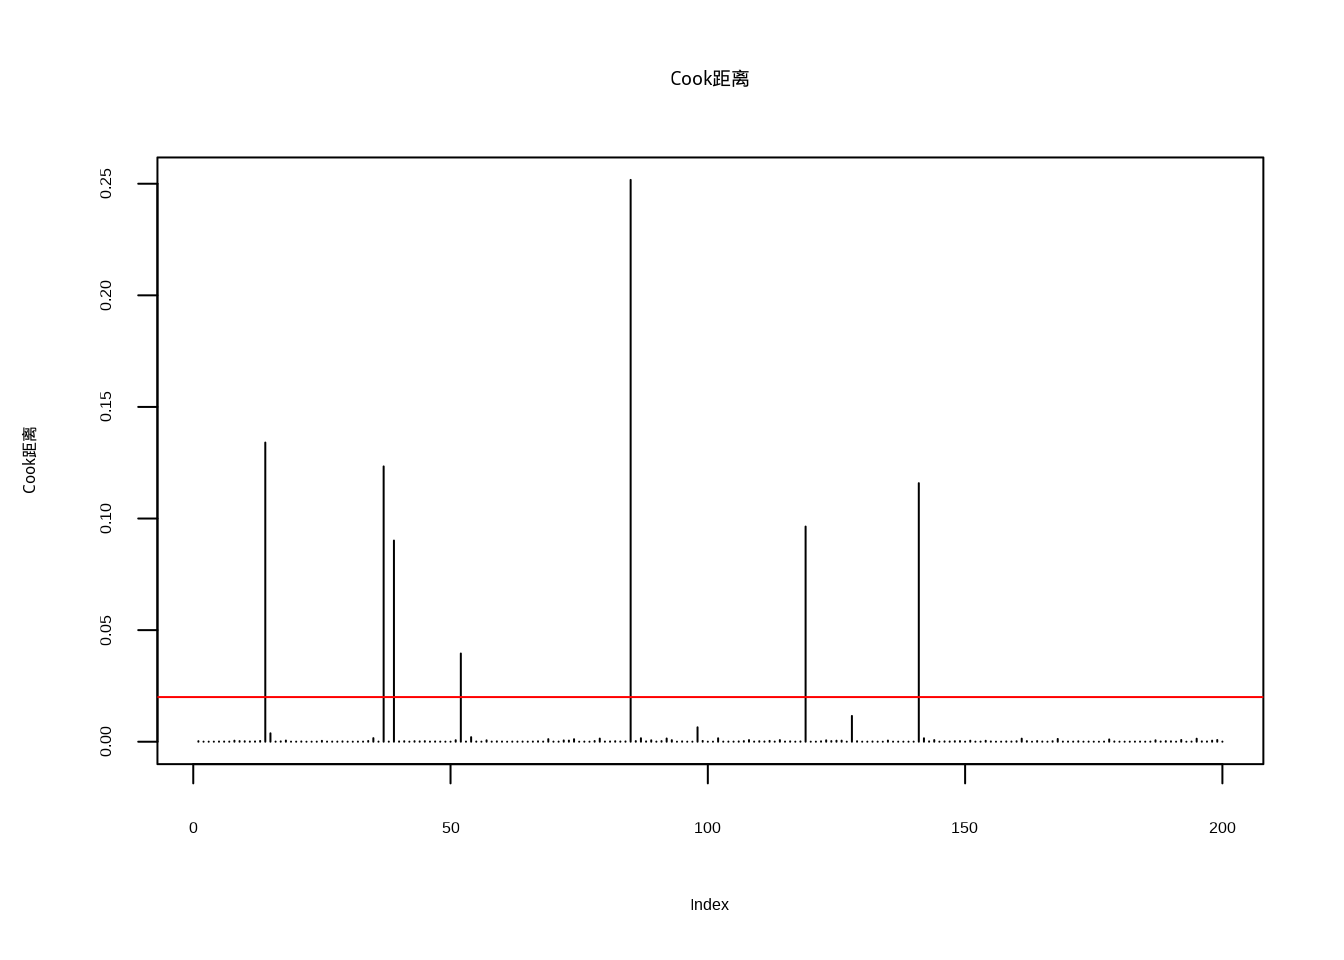
\includegraphics{03-summary_statistics_files/figure-latex/unnamed-chunk-12-1} 

}

\caption{树木胸径分布的直方图,展示右偏分布特征。红色虚线表示均值,蓝色虚线表示中位数,均值大于中位数表明分布向右偏斜。}\label{fig:unnamed-chunk-12}
\end{figure}

正偏度(通常大于0.5)表明分布向右偏斜,意味着有较多的小树和少数大树。在图形上,右偏分布的右侧尾部较长,均值大于中位数。这种模式常见于年龄结构年轻的种群。

\textbf{峰度}:

\textbf{数学定义}:样本峰度定义为四阶中心矩与标准差四次方的比值:

\[g_2 = \frac{\frac{1}{n}\sum_{i=1}^{n}(x_i - \bar{x})^4}{s^4} - 3\]

其中减去3是为了使正态分布的峰度为0。峰度大于0表示尖峰分布,小于0表示平峰分布。

峰度描述了分布的尖峰程度和尾部厚度。在研究极端生态事件时特别重要:

\begin{Shaded}
\begin{Highlighting}[]
\CommentTok{\# 模拟两种不同的物种多度分布}
\CommentTok{\# 分布A:尖峰分布(高峰度)}
\NormalTok{abundance\_a }\OtherTok{\textless{}{-}} \FunctionTok{c}\NormalTok{(}\FunctionTok{rep}\NormalTok{(}\DecValTok{10}\NormalTok{, }\DecValTok{8}\NormalTok{), }\FunctionTok{rep}\NormalTok{(}\DecValTok{15}\NormalTok{, }\DecValTok{2}\NormalTok{), }\FunctionTok{rep}\NormalTok{(}\DecValTok{20}\NormalTok{, }\DecValTok{25}\NormalTok{), }\FunctionTok{rep}\NormalTok{(}\DecValTok{25}\NormalTok{, }\DecValTok{2}\NormalTok{), }\FunctionTok{rep}\NormalTok{(}\DecValTok{30}\NormalTok{, }\DecValTok{8}\NormalTok{))}
\CommentTok{\# 分布B:平峰分布(低峰度)}
\NormalTok{abundance\_b }\OtherTok{\textless{}{-}} \FunctionTok{runif}\NormalTok{(}\DecValTok{45}\NormalTok{, }\DecValTok{10}\NormalTok{, }\DecValTok{30}\NormalTok{)}

\CommentTok{\# 计算峰度}
\NormalTok{kurtosis\_a }\OtherTok{\textless{}{-}} \FunctionTok{kurtosis}\NormalTok{(abundance\_a)}
\NormalTok{kurtosis\_b }\OtherTok{\textless{}{-}} \FunctionTok{kurtosis}\NormalTok{(abundance\_b)}

\FunctionTok{cat}\NormalTok{(}\StringTok{"物种A多度分布的峰度:"}\NormalTok{, }\FunctionTok{round}\NormalTok{(kurtosis\_a, }\DecValTok{2}\NormalTok{), }\StringTok{"}\SpecialCharTok{\textbackslash{}n}\StringTok{"}\NormalTok{,}
    \StringTok{"物种B多度分布的峰度:"}\NormalTok{, }\FunctionTok{round}\NormalTok{(kurtosis\_b, }\DecValTok{2}\NormalTok{), }\StringTok{"}\SpecialCharTok{\textbackslash{}n}\StringTok{"}\NormalTok{,}
    \AttributeTok{sep =} \StringTok{""}\NormalTok{)}
\end{Highlighting}
\end{Shaded}

\begin{verbatim}
## 物种A多度分布的峰度:2.53
## 物种B多度分布的峰度:2.06
\end{verbatim}

\begin{Shaded}
\begin{Highlighting}[]
\CommentTok{\# 正态分布的峰度为3,大于3表示尖峰,小于3表示平峰}
\FunctionTok{cat}\NormalTok{(}\StringTok{"物种A相对于正态分布的峰度:"}\NormalTok{, }\FunctionTok{round}\NormalTok{(kurtosis\_a }\SpecialCharTok{{-}} \DecValTok{3}\NormalTok{, }\DecValTok{2}\NormalTok{), }\StringTok{"}\SpecialCharTok{\textbackslash{}n}\StringTok{"}\NormalTok{,}
    \StringTok{"物种B相对于正态分布的峰度:"}\NormalTok{, }\FunctionTok{round}\NormalTok{(kurtosis\_b }\SpecialCharTok{{-}} \DecValTok{3}\NormalTok{, }\DecValTok{2}\NormalTok{), }\StringTok{"}\SpecialCharTok{\textbackslash{}n}\StringTok{"}\NormalTok{,}
    \AttributeTok{sep =} \StringTok{""}\NormalTok{)}
\end{Highlighting}
\end{Shaded}

\begin{verbatim}
## 物种A相对于正态分布的峰度:-0.47
## 物种B相对于正态分布的峰度:-0.94
\end{verbatim}

高峰度(大于3)表明分布更加尖峰,数据集中在均值附近,尾部较厚,意味着极端值(稀有物种)的出现概率较高。低峰度(小于3)表明分布更加平缓,数据分散,极端值较少。

\textbf{矩的概念}:

\textbf{数学定义}:对于一组观测值 \(x_1, x_2, \ldots, x_n\),第 \(k\) 阶样本矩定义为:

\[m_k = \frac{1}{n}\sum_{i=1}^{n}(x_i - \bar{x})^k\]

\begin{itemize}
\tightlist
\item
  一阶矩(\(k=1\)):均值,描述分布中心位置
\item
  二阶矩(\(k=2\)):方差,描述分布离散程度
\item
  三阶矩(\(k=3\)):偏度,描述分布不对称性
\item
  四阶矩(\(k=4\)):峰度,描述分布尖峰程度
\end{itemize}

矩提供了描述分布特征的系统框架。让我们用一个完整的例子来展示四个主要矩:

\begin{Shaded}
\begin{Highlighting}[]
\CommentTok{\# 研究湿地中不同水鸟物种的个体数量}
\NormalTok{waterbird\_counts }\OtherTok{\textless{}{-}} \FunctionTok{c}\NormalTok{(}\DecValTok{2}\NormalTok{, }\DecValTok{3}\NormalTok{, }\DecValTok{4}\NormalTok{, }\DecValTok{5}\NormalTok{, }\DecValTok{6}\NormalTok{, }\DecValTok{7}\NormalTok{, }\DecValTok{8}\NormalTok{, }\DecValTok{9}\NormalTok{, }\DecValTok{10}\NormalTok{, }\DecValTok{12}\NormalTok{, }\DecValTok{15}\NormalTok{, }\DecValTok{20}\NormalTok{, }\DecValTok{25}\NormalTok{, }\DecValTok{35}\NormalTok{, }\DecValTok{50}\NormalTok{)}

\CommentTok{\# 计算四个主要矩}
\NormalTok{mean\_count }\OtherTok{\textless{}{-}} \FunctionTok{mean}\NormalTok{(waterbird\_counts) }\CommentTok{\# 一阶矩:均值}
\NormalTok{variance\_count }\OtherTok{\textless{}{-}} \FunctionTok{var}\NormalTok{(waterbird\_counts) }\CommentTok{\# 二阶矩:方差}
\NormalTok{skewness\_count }\OtherTok{\textless{}{-}} \FunctionTok{skewness}\NormalTok{(waterbird\_counts) }\CommentTok{\# 三阶矩:偏度}
\NormalTok{kurtosis\_count }\OtherTok{\textless{}{-}} \FunctionTok{kurtosis}\NormalTok{(waterbird\_counts) }\CommentTok{\# 四阶矩:峰度}

\FunctionTok{cat}\NormalTok{(}\StringTok{"一阶矩(均值):"}\NormalTok{, }\FunctionTok{round}\NormalTok{(mean\_count, }\DecValTok{2}\NormalTok{), }\StringTok{"}\SpecialCharTok{\textbackslash{}n}\StringTok{"}\NormalTok{,}
    \StringTok{"二阶矩(方差):"}\NormalTok{, }\FunctionTok{round}\NormalTok{(variance\_count, }\DecValTok{2}\NormalTok{), }\StringTok{"}\SpecialCharTok{\textbackslash{}n}\StringTok{"}\NormalTok{,}
    \StringTok{"三阶矩(偏度):"}\NormalTok{, }\FunctionTok{round}\NormalTok{(skewness\_count, }\DecValTok{2}\NormalTok{), }\StringTok{"}\SpecialCharTok{\textbackslash{}n}\StringTok{"}\NormalTok{,}
    \StringTok{"四阶矩(峰度):"}\NormalTok{, }\FunctionTok{round}\NormalTok{(kurtosis\_count, }\DecValTok{2}\NormalTok{), }\StringTok{"}\SpecialCharTok{\textbackslash{}n}\StringTok{"}\NormalTok{,}
    \AttributeTok{sep =} \StringTok{""}\NormalTok{)}
\end{Highlighting}
\end{Shaded}

\begin{verbatim}
## 一阶矩(均值):14.07
## 二阶矩(方差):181.07
## 三阶矩(偏度):1.54
## 四阶矩(峰度):4.52
\end{verbatim}

\begin{Shaded}
\begin{Highlighting}[]
\CommentTok{\# 综合描述分布特征}
\FunctionTok{cat}\NormalTok{(}\StringTok{"}\SpecialCharTok{\textbackslash{}n}\StringTok{水鸟物种个体数量分布特征:}\SpecialCharTok{\textbackslash{}n}\StringTok{"}\NormalTok{,}
    \StringTok{"{-} 平均每个物种有"}\NormalTok{, }\FunctionTok{round}\NormalTok{(mean\_count, }\DecValTok{1}\NormalTok{), }\StringTok{"个个体}\SpecialCharTok{\textbackslash{}n}\StringTok{"}\NormalTok{,}
    \StringTok{"{-} 个体数量变异较大(方差="}\NormalTok{, }\FunctionTok{round}\NormalTok{(variance\_count, }\DecValTok{1}\NormalTok{), }\StringTok{")}\SpecialCharTok{\textbackslash{}n}\StringTok{"}\NormalTok{,}
    \AttributeTok{sep =} \StringTok{""}\NormalTok{)}
\end{Highlighting}
\end{Shaded}

\begin{verbatim}
## 
## 水鸟物种个体数量分布特征:
## - 平均每个物种有14.1个个体
## - 个体数量变异较大(方差=181.1)
\end{verbatim}

\begin{Shaded}
\begin{Highlighting}[]
\ControlFlowTok{if}\NormalTok{ (skewness\_count }\SpecialCharTok{\textgreater{}} \FloatTok{0.5}\NormalTok{) \{}
  \FunctionTok{cat}\NormalTok{(}\StringTok{"{-} 分布右偏,表明少数物种具有大量个体}\SpecialCharTok{\textbackslash{}n}\StringTok{"}\NormalTok{)}
\NormalTok{\} }\ControlFlowTok{else} \ControlFlowTok{if}\NormalTok{ (skewness\_count }\SpecialCharTok{\textless{}} \SpecialCharTok{{-}}\FloatTok{0.5}\NormalTok{) \{}
  \FunctionTok{cat}\NormalTok{(}\StringTok{"{-} 分布左偏,表明多数物种个体数量较少}\SpecialCharTok{\textbackslash{}n}\StringTok{"}\NormalTok{)}
\NormalTok{\} }\ControlFlowTok{else}\NormalTok{ \{}
  \FunctionTok{cat}\NormalTok{(}\StringTok{"{-} 分布基本对称}\SpecialCharTok{\textbackslash{}n}\StringTok{"}\NormalTok{)}
\NormalTok{\}}
\end{Highlighting}
\end{Shaded}

\begin{verbatim}
## - 分布右偏,表明少数物种具有大量个体
\end{verbatim}

\begin{Shaded}
\begin{Highlighting}[]
\ControlFlowTok{if}\NormalTok{ (kurtosis\_count }\SpecialCharTok{\textgreater{}} \DecValTok{3}\NormalTok{) \{}
  \FunctionTok{cat}\NormalTok{(}\StringTok{"{-} 分布尖峰,表明极端多度物种出现概率较高}\SpecialCharTok{\textbackslash{}n}\StringTok{"}\NormalTok{)}
\NormalTok{\} }\ControlFlowTok{else}\NormalTok{ \{}
  \FunctionTok{cat}\NormalTok{(}\StringTok{"{-} 分布相对平缓}\SpecialCharTok{\textbackslash{}n}\StringTok{"}\NormalTok{)}
\NormalTok{\}}
\end{Highlighting}
\end{Shaded}

\begin{verbatim}
## - 分布尖峰,表明极端多度物种出现概率较高
\end{verbatim}

这四个矩共同描述了水鸟物种多度分布的整体特征:均值告诉我们典型的多度水平,方差描述多度的变异程度,偏度揭示分布的对称性,峰度反映极端多度物种的出现概率。

在生态学研究中,理解这些分布形状特征至关重要。例如,右偏的物种多度分布通常表明群落由少数优势物种和多数稀有物种组成;高峰度的环境因子分布可能预示着极端气候事件的发生;偏斜的个体大小分布可能反映了种内竞争或资源分配的不均等性。通过矩分析,我们能够从简单的数值描述深入到对生态过程的理解。

\hypertarget{ux7edfux8ba1ux6982ux5ff5ux5728ux6982ux7387ux5206ux5e03ux56feux4e0aux7684ux53efux89c6ux5316}{%
\subsection{统计概念在概率分布图上的可视化}\label{ux7edfux8ba1ux6982ux5ff5ux5728ux6982ux7387ux5206ux5e03ux56feux4e0aux7684ux53efux89c6ux5316}}

为了更好地理解这些统计概念,让我们在一个典型的概率分布图上可视化它们:

\begin{Shaded}
\begin{Highlighting}[]
\CommentTok{\# 创建一个综合的可视化,展示所有统计概念}
\FunctionTok{library}\NormalTok{(ggplot2)}
\FunctionTok{library}\NormalTok{(gridExtra)}

\CommentTok{\# 生成正态分布数据}
\FunctionTok{set.seed}\NormalTok{(}\DecValTok{123}\NormalTok{)}
\NormalTok{x }\OtherTok{\textless{}{-}} \FunctionTok{seq}\NormalTok{(}\SpecialCharTok{{-}}\DecValTok{4}\NormalTok{, }\DecValTok{4}\NormalTok{, }\AttributeTok{length.out =} \DecValTok{1000}\NormalTok{)}
\NormalTok{y }\OtherTok{\textless{}{-}} \FunctionTok{dnorm}\NormalTok{(x)}

\CommentTok{\# 创建基础分布图}
\NormalTok{base\_plot }\OtherTok{\textless{}{-}} \FunctionTok{ggplot}\NormalTok{(}\FunctionTok{data.frame}\NormalTok{(}\AttributeTok{x =}\NormalTok{ x, }\AttributeTok{y =}\NormalTok{ y), }\FunctionTok{aes}\NormalTok{(}\AttributeTok{x =}\NormalTok{ x, }\AttributeTok{y =}\NormalTok{ y)) }\SpecialCharTok{+}
  \FunctionTok{geom\_line}\NormalTok{(}\AttributeTok{color =} \StringTok{"blue"}\NormalTok{, }\AttributeTok{linewidth =} \DecValTok{1}\NormalTok{) }\SpecialCharTok{+}
  \FunctionTok{labs}\NormalTok{(}
    \AttributeTok{title =} \StringTok{"统计概念在正态分布上的可视化"}\NormalTok{,}
    \AttributeTok{x =} \StringTok{"变量值"}\NormalTok{, }\AttributeTok{y =} \StringTok{"概率密度"}
\NormalTok{  ) }\SpecialCharTok{+}
  \FunctionTok{theme\_minimal}\NormalTok{()}

\CommentTok{\# 添加均值线}
\NormalTok{mean\_plot }\OtherTok{\textless{}{-}}\NormalTok{ base\_plot }\SpecialCharTok{+}
  \FunctionTok{geom\_vline}\NormalTok{(}\AttributeTok{xintercept =} \DecValTok{0}\NormalTok{, }\AttributeTok{color =} \StringTok{"red"}\NormalTok{,}
             \AttributeTok{linewidth =} \DecValTok{1}\NormalTok{, }\AttributeTok{linetype =} \StringTok{"solid"}\NormalTok{) }\SpecialCharTok{+}
  \FunctionTok{annotate}\NormalTok{(}\StringTok{"text"}\NormalTok{, }\AttributeTok{x =} \DecValTok{0}\NormalTok{, }\AttributeTok{y =} \FunctionTok{max}\NormalTok{(y) }\SpecialCharTok{*} \FloatTok{0.9}\NormalTok{,}
           \AttributeTok{label =} \StringTok{"均值"}\NormalTok{, }\AttributeTok{color =} \StringTok{"red"}\NormalTok{, }\AttributeTok{vjust =} \SpecialCharTok{{-}}\DecValTok{1}\NormalTok{)}

\CommentTok{\# 添加标准差范围}
\NormalTok{sd\_plot }\OtherTok{\textless{}{-}}\NormalTok{ mean\_plot }\SpecialCharTok{+}
  \FunctionTok{geom\_vline}\NormalTok{(}\AttributeTok{xintercept =} \FunctionTok{c}\NormalTok{(}\SpecialCharTok{{-}}\DecValTok{1}\NormalTok{, }\DecValTok{1}\NormalTok{), }\AttributeTok{color =} \StringTok{"orange"}\NormalTok{,}
             \AttributeTok{linewidth =} \FloatTok{0.8}\NormalTok{, }\AttributeTok{linetype =} \StringTok{"dashed"}\NormalTok{) }\SpecialCharTok{+}
  \FunctionTok{annotate}\NormalTok{(}\StringTok{"text"}\NormalTok{, }\AttributeTok{x =} \SpecialCharTok{{-}}\DecValTok{1}\NormalTok{, }\AttributeTok{y =} \FunctionTok{max}\NormalTok{(y) }\SpecialCharTok{*} \FloatTok{0.8}\NormalTok{,}
           \AttributeTok{label =} \StringTok{"{-}1σ"}\NormalTok{, }\AttributeTok{color =} \StringTok{"orange"}\NormalTok{, }\AttributeTok{vjust =} \SpecialCharTok{{-}}\DecValTok{1}\NormalTok{) }\SpecialCharTok{+}
  \FunctionTok{annotate}\NormalTok{(}\StringTok{"text"}\NormalTok{, }\AttributeTok{x =} \DecValTok{1}\NormalTok{, }\AttributeTok{y =} \FunctionTok{max}\NormalTok{(y) }\SpecialCharTok{*} \FloatTok{0.8}\NormalTok{,}
           \AttributeTok{label =} \StringTok{"+1σ"}\NormalTok{, }\AttributeTok{color =} \StringTok{"orange"}\NormalTok{, }\AttributeTok{vjust =} \SpecialCharTok{{-}}\DecValTok{1}\NormalTok{) }\SpecialCharTok{+}
  \FunctionTok{geom\_segment}\NormalTok{(}\FunctionTok{aes}\NormalTok{(}\AttributeTok{x =} \SpecialCharTok{{-}}\DecValTok{1}\NormalTok{, }\AttributeTok{y =} \FloatTok{0.1}\NormalTok{, }\AttributeTok{xend =} \DecValTok{1}\NormalTok{, }\AttributeTok{yend =} \FloatTok{0.1}\NormalTok{),}
    \AttributeTok{color =} \StringTok{"green"}\NormalTok{, }\AttributeTok{linewidth =} \DecValTok{2}\NormalTok{, }\AttributeTok{arrow =} \FunctionTok{arrow}\NormalTok{(}\AttributeTok{ends =} \StringTok{"both"}\NormalTok{)}
\NormalTok{  ) }\SpecialCharTok{+}
  \FunctionTok{annotate}\NormalTok{(}\StringTok{"text"}\NormalTok{, }\AttributeTok{x =} \DecValTok{0}\NormalTok{, }\AttributeTok{y =} \FloatTok{0.15}\NormalTok{, }\AttributeTok{label =} \StringTok{"标准差范围"}\NormalTok{, }\AttributeTok{color =} \StringTok{"green"}\NormalTok{)}

\CommentTok{\# 显示图形}
\FunctionTok{print}\NormalTok{(sd\_plot)}
\end{Highlighting}
\end{Shaded}

\begin{figure}

{\centering \includegraphics{03-summary_statistics_files/figure-latex/unnamed-chunk-15-1} 

}

\caption{统计概念在正态分布上的可视化。红色垂直线表示均值,橙色虚线表示±1个标准差的范围,绿色箭头表示标准差的实际跨度。}\label{fig:unnamed-chunk-15}
\end{figure}

这个可视化展示了:
- \textbf{红色垂直线}:均值(分布的中心位置)
- \textbf{橙色虚线}:±1个标准差的范围
- \textbf{绿色箭头}:标准差的实际跨度

\hypertarget{ux6807ux51c6ux8befux7684ux53efux89c6ux5316ux7406ux89e3}{%
\subsection{标准误的可视化理解}\label{ux6807ux51c6ux8befux7684ux53efux89c6ux5316ux7406ux89e3}}

为了理解标准误的概念,让我们通过抽样模拟来展示标准误的意义:

\begin{Shaded}
\begin{Highlighting}[]
\CommentTok{\# 标准误的可视化:抽样变异性}
\FunctionTok{set.seed}\NormalTok{(}\DecValTok{456}\NormalTok{)}
\CommentTok{\# 假设总体服从正态分布}
\NormalTok{population }\OtherTok{\textless{}{-}} \FunctionTok{rnorm}\NormalTok{(}\DecValTok{10000}\NormalTok{, }\AttributeTok{mean =} \DecValTok{50}\NormalTok{, }\AttributeTok{sd =} \DecValTok{10}\NormalTok{)}

\CommentTok{\# 进行多次抽样}
\NormalTok{n\_samples }\OtherTok{\textless{}{-}} \DecValTok{100}
\NormalTok{sample\_size }\OtherTok{\textless{}{-}} \DecValTok{30}
\NormalTok{sample\_means }\OtherTok{\textless{}{-}} \FunctionTok{numeric}\NormalTok{(n\_samples)}
\NormalTok{sample\_ses }\OtherTok{\textless{}{-}} \FunctionTok{numeric}\NormalTok{(n\_samples)}

\ControlFlowTok{for}\NormalTok{ (i }\ControlFlowTok{in} \DecValTok{1}\SpecialCharTok{:}\NormalTok{n\_samples) \{}
\NormalTok{  sample\_data }\OtherTok{\textless{}{-}} \FunctionTok{sample}\NormalTok{(population, sample\_size)}
\NormalTok{  sample\_means[i] }\OtherTok{\textless{}{-}} \FunctionTok{mean}\NormalTok{(sample\_data)}
\NormalTok{  sample\_ses[i] }\OtherTok{\textless{}{-}} \FunctionTok{sd}\NormalTok{(sample\_data) }\SpecialCharTok{/} \FunctionTok{sqrt}\NormalTok{(sample\_size)}
\NormalTok{\}}

\CommentTok{\# 创建可视化}
\FunctionTok{par}\NormalTok{(}\AttributeTok{mfrow =} \FunctionTok{c}\NormalTok{(}\DecValTok{1}\NormalTok{, }\DecValTok{2}\NormalTok{))}

\CommentTok{\# 左图:样本均值的分布}
\FunctionTok{hist}\NormalTok{(sample\_means,}
  \AttributeTok{breaks =} \DecValTok{20}\NormalTok{, }\AttributeTok{col =} \StringTok{"lightblue"}\NormalTok{, }\AttributeTok{border =} \StringTok{"darkblue"}\NormalTok{,}
  \AttributeTok{main =} \StringTok{"样本均值的分布"}\NormalTok{, }\AttributeTok{xlab =} \StringTok{"样本均值"}\NormalTok{, }\AttributeTok{ylab =} \StringTok{"频率"}
\NormalTok{)}
\FunctionTok{abline}\NormalTok{(}\AttributeTok{v =} \FunctionTok{mean}\NormalTok{(population), }\AttributeTok{col =} \StringTok{"red"}\NormalTok{, }\AttributeTok{lwd =} \DecValTok{3}\NormalTok{, }\AttributeTok{lty =} \DecValTok{2}\NormalTok{)}
\FunctionTok{legend}\NormalTok{(}\StringTok{"topright"}\NormalTok{, }\AttributeTok{legend =} \StringTok{"总体均值"}\NormalTok{, }\AttributeTok{col =} \StringTok{"red"}\NormalTok{, }\AttributeTok{lwd =} \DecValTok{3}\NormalTok{, }\AttributeTok{lty =} \DecValTok{2}\NormalTok{)}

\CommentTok{\# 右图:标准误与样本均值的关系}
\FunctionTok{plot}\NormalTok{(sample\_means, sample\_ses,}
  \AttributeTok{pch =} \DecValTok{16}\NormalTok{, }\AttributeTok{col =} \StringTok{"darkgreen"}\NormalTok{,}
  \AttributeTok{xlab =} \StringTok{"样本均值"}\NormalTok{, }\AttributeTok{ylab =} \StringTok{"标准误"}\NormalTok{,}
  \AttributeTok{main =} \StringTok{"标准误与样本均值的关系"}
\NormalTok{)}
\FunctionTok{abline}\NormalTok{(}\AttributeTok{h =} \FunctionTok{mean}\NormalTok{(sample\_ses), }\AttributeTok{col =} \StringTok{"orange"}\NormalTok{, }\AttributeTok{lwd =} \DecValTok{2}\NormalTok{, }\AttributeTok{lty =} \DecValTok{2}\NormalTok{)}
\FunctionTok{legend}\NormalTok{(}\StringTok{"topright"}\NormalTok{, }\AttributeTok{legend =} \StringTok{"平均标准误"}\NormalTok{, }\AttributeTok{col =} \StringTok{"orange"}\NormalTok{, }\AttributeTok{lwd =} \DecValTok{2}\NormalTok{, }\AttributeTok{lty =} \DecValTok{2}\NormalTok{)}
\end{Highlighting}
\end{Shaded}

\begin{figure}

{\centering 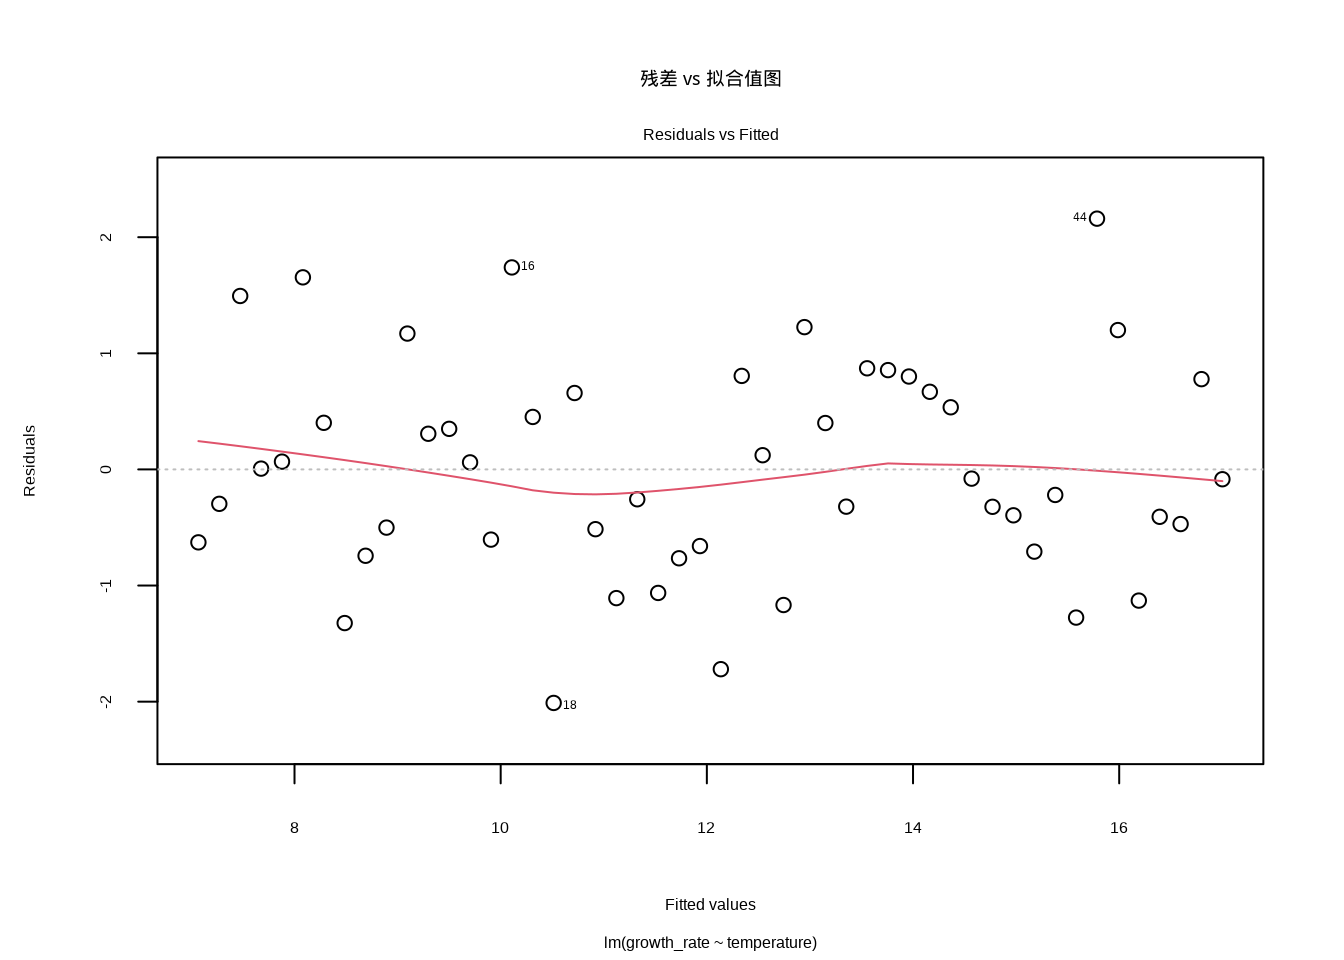
\includegraphics{03-summary_statistics_files/figure-latex/unnamed-chunk-16-1} 

}

\caption{标准误的可视化分析。左图显示样本均值的分布,右图展示标准误与样本均值的关系。红色虚线表示总体均值,橙色虚线表示平均标准误。}\label{fig:unnamed-chunk-16}
\end{figure}

\begin{Shaded}
\begin{Highlighting}[]
\CommentTok{\# 添加置信区间示例}
\NormalTok{sample\_mean }\OtherTok{\textless{}{-}} \FunctionTok{mean}\NormalTok{(sample\_means)}
\NormalTok{sample\_se }\OtherTok{\textless{}{-}} \FunctionTok{sd}\NormalTok{(sample\_means)}
\NormalTok{ci\_lower }\OtherTok{\textless{}{-}}\NormalTok{ sample\_mean }\SpecialCharTok{{-}} \FloatTok{1.96} \SpecialCharTok{*}\NormalTok{ sample\_se}
\NormalTok{ci\_upper }\OtherTok{\textless{}{-}}\NormalTok{ sample\_mean }\SpecialCharTok{+} \FloatTok{1.96} \SpecialCharTok{*}\NormalTok{ sample\_se}

\FunctionTok{cat}\NormalTok{(}\StringTok{"总体均值:"}\NormalTok{, }\FunctionTok{round}\NormalTok{(}\FunctionTok{mean}\NormalTok{(population), }\DecValTok{2}\NormalTok{), }\StringTok{"}\SpecialCharTok{\textbackslash{}n}\StringTok{"}\NormalTok{,}
    \StringTok{"样本均值的均值:"}\NormalTok{, }\FunctionTok{round}\NormalTok{(sample\_mean, }\DecValTok{2}\NormalTok{), }\StringTok{"}\SpecialCharTok{\textbackslash{}n}\StringTok{"}\NormalTok{,}
    \StringTok{"样本均值的标准误:"}\NormalTok{, }\FunctionTok{round}\NormalTok{(sample\_se, }\DecValTok{2}\NormalTok{), }\StringTok{"}\SpecialCharTok{\textbackslash{}n}\StringTok{"}\NormalTok{,}
    \StringTok{"95\%置信区间:[ "}\NormalTok{, }\FunctionTok{round}\NormalTok{(ci\_lower, }\DecValTok{2}\NormalTok{), }\StringTok{", "}\NormalTok{, }\FunctionTok{round}\NormalTok{(ci\_upper, }\DecValTok{2}\NormalTok{), }\StringTok{" ]}\SpecialCharTok{\textbackslash{}n}\StringTok{"}\NormalTok{,}
    \AttributeTok{sep =} \StringTok{""}\NormalTok{)}
\end{Highlighting}
\end{Shaded}

\begin{verbatim}
## 总体均值:50.16
## 样本均值的均值:50.17
## 样本均值的标准误:2.04
## 95%置信区间:[ 46.17, 54.17 ]
\end{verbatim}

这个可视化帮助我们理解:
- \textbf{左图}:多次抽样的样本均值围绕总体均值波动,其分布的标准差就是标准误
- \textbf{右图}:标准误反映了样本均值作为总体均值估计的精确程度
- \textbf{置信区间}:基于标准误构建的区间包含了总体均值的概率为95\%

\hypertarget{ux4e0dux540cux53c2ux6570ux503cux7684ux5206ux5e03ux5f62ux72b6ux6bd4ux8f83}{%
\subsection{不同参数值的分布形状比较}\label{ux4e0dux540cux53c2ux6570ux503cux7684ux5206ux5e03ux5f62ux72b6ux6bd4ux8f83}}

现在让我们比较不同统计参数值对应的分布形状:

\begin{Shaded}
\begin{Highlighting}[]
\CommentTok{\# 比较不同均值的分布}
\NormalTok{x\_range }\OtherTok{\textless{}{-}} \FunctionTok{seq}\NormalTok{(}\SpecialCharTok{{-}}\DecValTok{5}\NormalTok{, }\DecValTok{10}\NormalTok{, }\AttributeTok{length.out =} \DecValTok{1000}\NormalTok{)}
\NormalTok{df\_means }\OtherTok{\textless{}{-}} \FunctionTok{data.frame}\NormalTok{(}
  \AttributeTok{x =} \FunctionTok{rep}\NormalTok{(x\_range, }\DecValTok{3}\NormalTok{),}
  \AttributeTok{y =} \FunctionTok{c}\NormalTok{(}\FunctionTok{dnorm}\NormalTok{(x\_range, }\AttributeTok{mean =} \DecValTok{0}\NormalTok{),}
        \FunctionTok{dnorm}\NormalTok{(x\_range, }\AttributeTok{mean =} \DecValTok{2}\NormalTok{),}
        \FunctionTok{dnorm}\NormalTok{(x\_range, }\AttributeTok{mean =} \DecValTok{5}\NormalTok{)),}
  \AttributeTok{mean =} \FunctionTok{factor}\NormalTok{(}\FunctionTok{rep}\NormalTok{(}\FunctionTok{c}\NormalTok{(}\StringTok{"均值=0"}\NormalTok{, }\StringTok{"均值=2"}\NormalTok{, }\StringTok{"均值=5"}\NormalTok{), }\AttributeTok{each =} \DecValTok{1000}\NormalTok{))}
\NormalTok{)}

\NormalTok{mean\_comparison }\OtherTok{\textless{}{-}} \FunctionTok{ggplot}\NormalTok{(df\_means, }\FunctionTok{aes}\NormalTok{(}\AttributeTok{x =}\NormalTok{ x, }\AttributeTok{y =}\NormalTok{ y, }\AttributeTok{color =}\NormalTok{ mean)) }\SpecialCharTok{+}
  \FunctionTok{geom\_line}\NormalTok{(}\AttributeTok{linewidth =} \DecValTok{1}\NormalTok{) }\SpecialCharTok{+}
  \FunctionTok{labs}\NormalTok{(}
    \AttributeTok{title =} \StringTok{"不同均值的分布比较"}\NormalTok{,}
    \AttributeTok{x =} \StringTok{"变量值"}\NormalTok{, }\AttributeTok{y =} \StringTok{"概率密度"}\NormalTok{, }\AttributeTok{color =} \StringTok{"均值"}
\NormalTok{  ) }\SpecialCharTok{+}
  \FunctionTok{theme\_minimal}\NormalTok{() }\SpecialCharTok{+}
  \FunctionTok{scale\_color\_brewer}\NormalTok{(}\AttributeTok{palette =} \StringTok{"Set1"}\NormalTok{)}

\CommentTok{\# 比较不同标准差的分布}
\NormalTok{df\_sds }\OtherTok{\textless{}{-}} \FunctionTok{data.frame}\NormalTok{(}
  \AttributeTok{x =} \FunctionTok{rep}\NormalTok{(x\_range, }\DecValTok{3}\NormalTok{),}
  \AttributeTok{y =} \FunctionTok{c}\NormalTok{(}\FunctionTok{dnorm}\NormalTok{(x\_range, }\AttributeTok{sd =} \FloatTok{0.5}\NormalTok{),}
        \FunctionTok{dnorm}\NormalTok{(x\_range, }\AttributeTok{sd =} \DecValTok{1}\NormalTok{),}
        \FunctionTok{dnorm}\NormalTok{(x\_range, }\AttributeTok{sd =} \DecValTok{2}\NormalTok{)),}
  \AttributeTok{sd =} \FunctionTok{factor}\NormalTok{(}\FunctionTok{rep}\NormalTok{(}\FunctionTok{c}\NormalTok{(}\StringTok{"标准差=0.5"}\NormalTok{, }\StringTok{"标准差=1"}\NormalTok{, }\StringTok{"标准差=2"}\NormalTok{), }\AttributeTok{each =} \DecValTok{1000}\NormalTok{))}
\NormalTok{)}

\NormalTok{sd\_comparison }\OtherTok{\textless{}{-}} \FunctionTok{ggplot}\NormalTok{(df\_sds, }\FunctionTok{aes}\NormalTok{(}\AttributeTok{x =}\NormalTok{ x, }\AttributeTok{y =}\NormalTok{ y, }\AttributeTok{color =}\NormalTok{ sd)) }\SpecialCharTok{+}
  \FunctionTok{geom\_line}\NormalTok{(}\AttributeTok{linewidth =} \DecValTok{1}\NormalTok{) }\SpecialCharTok{+}
  \FunctionTok{labs}\NormalTok{(}
    \AttributeTok{title =} \StringTok{"不同标准差的分布比较"}\NormalTok{,}
    \AttributeTok{x =} \StringTok{"变量值"}\NormalTok{, }\AttributeTok{y =} \StringTok{"概率密度"}\NormalTok{, }\AttributeTok{color =} \StringTok{"标准差"}
\NormalTok{  ) }\SpecialCharTok{+}
  \FunctionTok{theme\_minimal}\NormalTok{() }\SpecialCharTok{+}
  \FunctionTok{scale\_color\_brewer}\NormalTok{(}\AttributeTok{palette =} \StringTok{"Set2"}\NormalTok{)}

\CommentTok{\# 比较不同偏度的分布(使用偏态分布)}
\FunctionTok{library}\NormalTok{(sn)}
\NormalTok{x\_skew }\OtherTok{\textless{}{-}} \FunctionTok{seq}\NormalTok{(}\SpecialCharTok{{-}}\DecValTok{3}\NormalTok{, }\DecValTok{8}\NormalTok{, }\AttributeTok{length.out =} \DecValTok{1000}\NormalTok{)}
\NormalTok{df\_skew }\OtherTok{\textless{}{-}} \FunctionTok{data.frame}\NormalTok{(}
  \AttributeTok{x =} \FunctionTok{rep}\NormalTok{(x\_skew, }\DecValTok{3}\NormalTok{),}
  \AttributeTok{y =} \FunctionTok{c}\NormalTok{(}\FunctionTok{dsn}\NormalTok{(x\_skew, }\AttributeTok{alpha =} \DecValTok{0}\NormalTok{), }\FunctionTok{dsn}\NormalTok{(x\_skew, }\AttributeTok{alpha =} \DecValTok{2}\NormalTok{), }\FunctionTok{dsn}\NormalTok{(x\_skew, }\AttributeTok{alpha =} \DecValTok{5}\NormalTok{)),}
  \AttributeTok{skewness =} \FunctionTok{factor}\NormalTok{(}\FunctionTok{rep}\NormalTok{(}\FunctionTok{c}\NormalTok{(}\StringTok{"偏度≈0"}\NormalTok{, }\StringTok{"偏度\textgreater{}0(右偏)"}\NormalTok{, }\StringTok{"偏度\textgreater{}\textgreater{}0(强右偏)"}\NormalTok{), }\AttributeTok{each =} \DecValTok{1000}\NormalTok{))}
\NormalTok{)}

\NormalTok{skew\_comparison }\OtherTok{\textless{}{-}} \FunctionTok{ggplot}\NormalTok{(df\_skew, }\FunctionTok{aes}\NormalTok{(}\AttributeTok{x =}\NormalTok{ x, }\AttributeTok{y =}\NormalTok{ y, }\AttributeTok{color =}\NormalTok{ skewness)) }\SpecialCharTok{+}
  \FunctionTok{geom\_line}\NormalTok{(}\AttributeTok{linewidth =} \DecValTok{1}\NormalTok{) }\SpecialCharTok{+}
  \FunctionTok{labs}\NormalTok{(}
    \AttributeTok{title =} \StringTok{"不同偏度的分布比较"}\NormalTok{,}
    \AttributeTok{x =} \StringTok{"变量值"}\NormalTok{, }\AttributeTok{y =} \StringTok{"概率密度"}\NormalTok{, }\AttributeTok{color =} \StringTok{"偏度"}
\NormalTok{  ) }\SpecialCharTok{+}
  \FunctionTok{theme\_minimal}\NormalTok{() }\SpecialCharTok{+}
  \FunctionTok{scale\_color\_brewer}\NormalTok{(}\AttributeTok{palette =} \StringTok{"Set3"}\NormalTok{)}

\CommentTok{\# 比较不同峰度的分布(使用t分布)}
\NormalTok{df\_kurtosis }\OtherTok{\textless{}{-}} \FunctionTok{data.frame}\NormalTok{(}
  \AttributeTok{x =} \FunctionTok{rep}\NormalTok{(x\_range, }\DecValTok{3}\NormalTok{),}
  \AttributeTok{y =} \FunctionTok{c}\NormalTok{(}\FunctionTok{dt}\NormalTok{(x\_range, }\AttributeTok{df =} \DecValTok{30}\NormalTok{),}
        \FunctionTok{dt}\NormalTok{(x\_range, }\AttributeTok{df =} \DecValTok{5}\NormalTok{),}
        \FunctionTok{dt}\NormalTok{(x\_range, }\AttributeTok{df =} \DecValTok{2}\NormalTok{)),}
  \AttributeTok{kurtosis =} \FunctionTok{factor}\NormalTok{(}\FunctionTok{rep}\NormalTok{(}\FunctionTok{c}\NormalTok{(}\StringTok{"峰度≈0"}\NormalTok{, }\StringTok{"峰度\textgreater{}0(尖峰)"}\NormalTok{, }\StringTok{"峰度\textgreater{}\textgreater{}0(强尖峰)"}\NormalTok{),}
                        \AttributeTok{each =} \DecValTok{1000}\NormalTok{))}
\NormalTok{)}

\NormalTok{kurtosis\_comparison }\OtherTok{\textless{}{-}} \FunctionTok{ggplot}\NormalTok{(df\_kurtosis,}
                              \FunctionTok{aes}\NormalTok{(}\AttributeTok{x =}\NormalTok{ x, }\AttributeTok{y =}\NormalTok{ y, }\AttributeTok{color =}\NormalTok{ kurtosis)) }\SpecialCharTok{+}
  \FunctionTok{geom\_line}\NormalTok{(}\AttributeTok{linewidth =} \DecValTok{1}\NormalTok{) }\SpecialCharTok{+}
  \FunctionTok{labs}\NormalTok{(}
    \AttributeTok{title =} \StringTok{"不同峰度的分布比较"}\NormalTok{,}
    \AttributeTok{x =} \StringTok{"变量值"}\NormalTok{, }\AttributeTok{y =} \StringTok{"概率密度"}\NormalTok{, }\AttributeTok{color =} \StringTok{"峰度"}
\NormalTok{  ) }\SpecialCharTok{+}
  \FunctionTok{theme\_minimal}\NormalTok{() }\SpecialCharTok{+}
  \FunctionTok{scale\_color\_brewer}\NormalTok{(}\AttributeTok{palette =} \StringTok{"Set1"}\NormalTok{)}

\CommentTok{\# 显示所有比较图}
\FunctionTok{grid.arrange}\NormalTok{(mean\_comparison, sd\_comparison,}
\NormalTok{             skew\_comparison, kurtosis\_comparison, }\AttributeTok{ncol =} \DecValTok{2}\NormalTok{)}
\end{Highlighting}
\end{Shaded}

\begin{figure}

{\centering 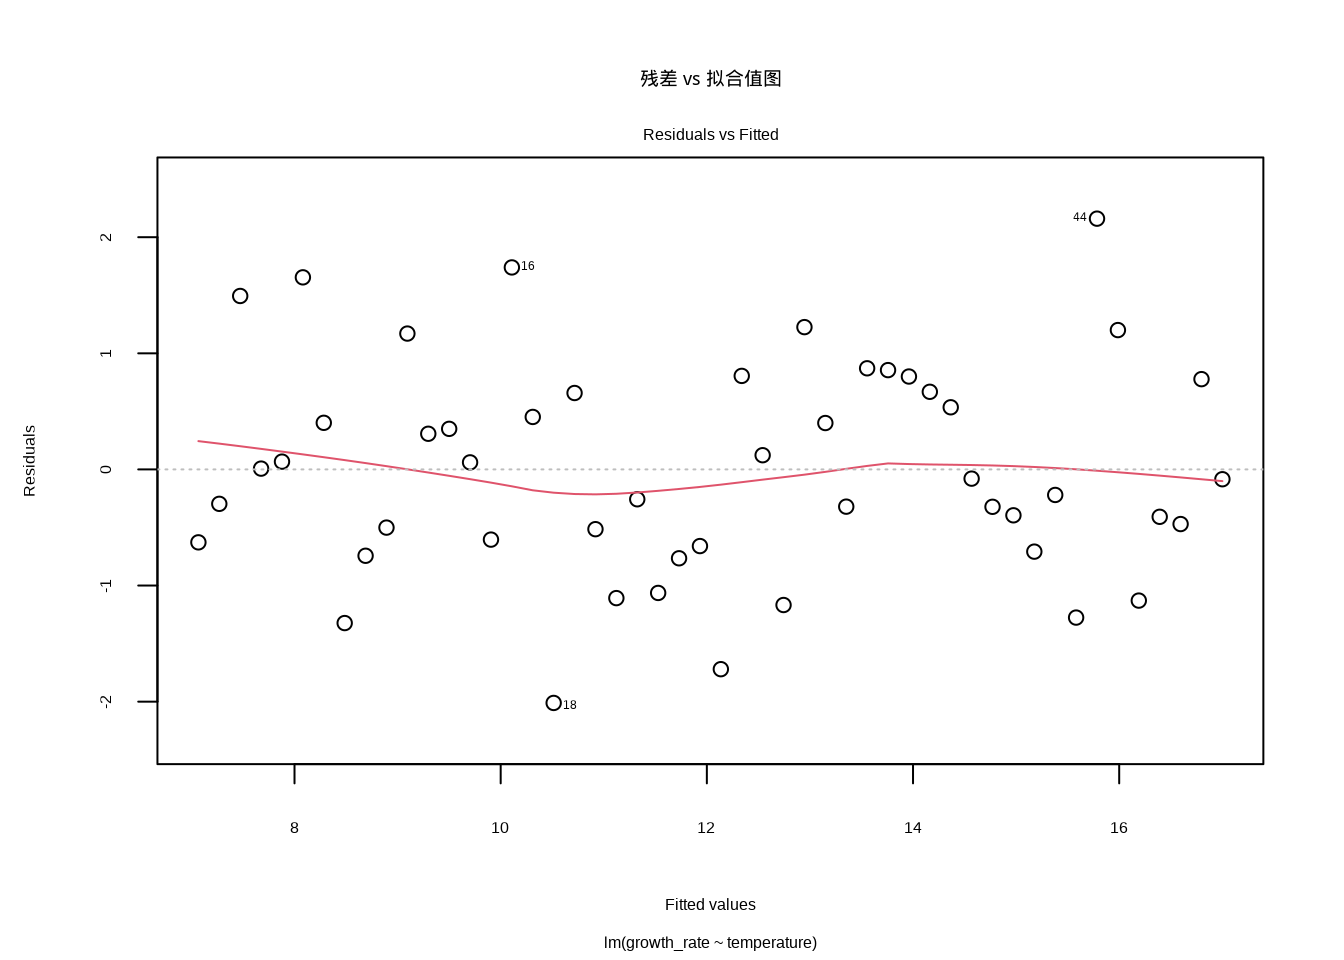
\includegraphics{03-summary_statistics_files/figure-latex/unnamed-chunk-17-1} 

}

\caption{不同统计参数值的分布形状比较。包括均值、标准差、偏度和峰度四个维度的分布特征对比,展示了统计参数对分布形状的影响。}\label{fig:unnamed-chunk-17}
\end{figure}

\hypertarget{ux751fux6001ux5b66ux610fux4e49ux603bux7ed3}{%
\subsection{生态学意义总结}\label{ux751fux6001ux5b66ux610fux4e49ux603bux7ed3}}

通过这些可视化,我们可以清楚地看到:

\textbf{均值的影响}:
- \textbf{大均值}:分布整体向右移动,对应生态学中较大的个体大小、较高的生物量等
- \textbf{小均值}:分布整体向左移动,对应较小的生态特征值

\textbf{方差/标准差的影响}:
- \textbf{大方差}:分布更加''矮胖'',数据分散,对应生态系统中个体间差异大、环境异质性高
- \textbf{小方差}:分布更加''瘦高'',数据集中,对应均质的生态系统

\textbf{偏度的影响}:
- \textbf{大正偏度}:分布右偏,右侧尾部较长,对应生态学中少数个体具有极大值(如优势物种)
- \textbf{大负偏度}:分布左偏,左侧尾部较长,对应多数个体具有较小值
- \textbf{零偏度}:对称分布,个体特征相对均匀

\textbf{峰度的影响}:
- \textbf{高峰度}:分布尖峰厚尾,数据集中在均值附近但极端值概率较高,对应生态系统中稳定状态但偶发极端事件
- \textbf{低峰度}:分布平峰薄尾,数据分散,极端值较少,对应生态系统状态波动较大但无极端事件

\textbf{标准误的意义}:
- \textbf{小标准误}:样本均值作为总体均值的估计更加精确,对应生态学中基于大样本的可靠推断
- \textbf{大标准误}:样本均值的估计不确定性较高,对应生态学中小样本研究的局限性

这些分布特征在生态学研究中具有重要的实际意义。例如:
- 物种多度分布通常呈现右偏,反映了少数优势物种和多数稀有物种的格局
- 环境因子的分布可能呈现高峰度,预示着极端气候事件的发生概率
- 个体大小的分布偏度可以反映种内竞争强度
- 群落多样性的分布方差可以指示生态系统的稳定性
- 基于标准误的置信区间为生态参数的估计提供了不确定性度量

通过理解这些统计概念在概率分布图上的表现,生态学家能够更准确地解读生态数据背后的模式和过程。

\hypertarget{ux73afux5883ux5f02ux8d28ux6027ux63cfux8ff0}{%
\section{环境异质性描述}\label{ux73afux5883ux5f02ux8d28ux6027ux63cfux8ff0}}

\hypertarget{ux73afux5883ux5f02ux8d28ux6027ux7684ux6982ux5ff5}{%
\subsection{环境异质性的概念}\label{ux73afux5883ux5f02ux8d28ux6027ux7684ux6982ux5ff5}}

环境异质性是指环境因子在空间或时间上的变异程度,是生态系统中至关重要的结构特征。想象一片森林生态系统,如果土壤养分在整个区域均匀分布,我们就说环境异质性低;如果某些区域土壤肥沃,某些区域贫瘠,我们就说环境异质性高。这种异质性深刻影响着物种的分布、群落的构建和生态系统的功能。

从生态学角度来看,环境异质性可以分为空间异质性和时间异质性。空间异质性体现在环境因子在不同位置的差异,比如山坡上部和下部的温度差异、河流上游和下游的水质差异。时间异质性则体现在环境因子随时间的变化,比如季节性的温度波动、年际间的降水量变化。

高环境异质性通常意味着更多的生态位机会,能够支持更高的物种多样性。例如,一个具有复杂地形和多种土壤类型的区域,往往比平坦均质的区域拥有更多的植物物种。相反,低环境异质性的环境往往被少数适应能力强的物种所主导。

\hypertarget{ux73afux5883ux5f02ux8d28ux6027ux7684ux53efux89c6ux5316ux7406ux89e3}{%
\subsection{环境异质性的可视化理解}\label{ux73afux5883ux5f02ux8d28ux6027ux7684ux53efux89c6ux5316ux7406ux89e3}}

为了更好地理解环境异质性的概念,我们可以通过图示来展示不同异质性水平的环境格局:

\begin{figure}

{\centering \includegraphics{03-summary_statistics_files/figure-latex/unnamed-chunk-18-1} 

}

\caption{环境异质性可视化分析。上图展示低环境异质性和高环境异质性的空间分布对比,下图通过箱线图比较两种异质性类型的土壤养分值分布。}\label{fig:unnamed-chunk-18}
\end{figure}

在低环境异质性的情况下,环境因子值在空间上相对均匀,没有明显的梯度或斑块化格局。而在高环境异质性的情况下,环境因子值呈现出明显的空间结构,可能表现为梯度变化、斑块分布或复杂的空间格局。

\hypertarget{ux73afux5883ux5f02ux8d28ux6027ux7684ux91cfux5316ux65b9ux6cd5}{%
\subsection{环境异质性的量化方法}\label{ux73afux5883ux5f02ux8d28ux6027ux7684ux91cfux5316ux65b9ux6cd5}}

\hypertarget{ux53d8ux5f02ux7cfbux6570coefficient-of-variation-cv}{%
\subsubsection{变异系数(Coefficient of Variation, CV)}\label{ux53d8ux5f02ux7cfbux6570coefficient-of-variation-cv}}

变异系数是描述环境因子相对变异程度的最基本统计量。其数学定义为标准差与均值的比值乘以100\%。变异系数的生态学意义在于它能够消除量纲的影响,使我们能够比较不同环境因子的变异程度。

在生态学研究中,变异系数被广泛应用于描述土壤养分、温度、湿度等环境因子的空间变异。例如,当我们研究一片森林中不同样方的土壤氮含量时,如果变异系数小于20\%,说明土壤氮含量相对均质;如果变异系数大于40\%,则表明土壤氮含量在空间上存在显著差异。这种变异模式可能反映了地形、植被覆盖或土壤形成过程的差异。

变异系数的优势在于计算简单、解释直观,但它无法提供关于变异空间结构的信息。因此,在需要深入了解环境异质性空间格局的研究中,通常需要结合其他更复杂的统计方法。

\hypertarget{morans-i-ux7a7aux95f4ux81eaux76f8ux5173ux6307ux6570}{%
\subsubsection{Moran's I 空间自相关指数}\label{morans-i-ux7a7aux95f4ux81eaux76f8ux5173ux6307ux6570}}

Moran's I 是量化环境因子空间自相关性的重要统计量,它衡量相邻位置环境因子值的相似程度。Moran's I 的取值范围在-1到+1之间,正值表示空间正相关(相似值聚集),负值表示空间负相关(相异值聚集),接近零表示空间随机分布。

\textbf{数学定义:}
\[I = \frac{n}{\sum_{i=1}^{n}\sum_{j=1}^{n}w_{ij}} \cdot \frac{\sum_{i=1}^{n}\sum_{j=1}^{n}w_{ij}(x_i - \bar{x})(x_j - \bar{x})}{\sum_{i=1}^{n}(x_i - \bar{x})^2}\]

其中:
- \(n\) 为观测点数量
- \(x_i\) 为第 \(i\) 个位置的观测值
- \(\bar{x}\) 为所有观测值的均值
- \(w_{ij}\) 为空间权重矩阵元素

\textbf{R代码实现:}

\begin{Shaded}
\begin{Highlighting}[]
\CommentTok{\# 示例数据:10个位置的温度观测值}
\NormalTok{temp\_data }\OtherTok{\textless{}{-}} \FunctionTok{c}\NormalTok{(}\FloatTok{15.2}\NormalTok{, }\FloatTok{16.1}\NormalTok{, }\FloatTok{15.8}\NormalTok{, }\FloatTok{16.3}\NormalTok{, }\FloatTok{15.9}\NormalTok{, }\FloatTok{16.0}\NormalTok{, }\FloatTok{15.7}\NormalTok{, }\FloatTok{16.2}\NormalTok{, }\FloatTok{15.6}\NormalTok{, }\FloatTok{16.1}\NormalTok{)}
\NormalTok{coords }\OtherTok{\textless{}{-}} \FunctionTok{data.frame}\NormalTok{(}\AttributeTok{x =} \DecValTok{1}\SpecialCharTok{:}\DecValTok{10}\NormalTok{, }\AttributeTok{y =} \FunctionTok{rep}\NormalTok{(}\DecValTok{1}\NormalTok{, }\DecValTok{10}\NormalTok{))}

\CommentTok{\# 计算Moran\textquotesingle{}s I}
\FunctionTok{library}\NormalTok{(spdep)}
\NormalTok{nb }\OtherTok{\textless{}{-}}\NormalTok{ spdep}\SpecialCharTok{::}\FunctionTok{knearneigh}\NormalTok{(}\FunctionTok{as.matrix}\NormalTok{(coords), }\AttributeTok{k =} \DecValTok{2}\NormalTok{)}
\NormalTok{listw }\OtherTok{\textless{}{-}}\NormalTok{ spdep}\SpecialCharTok{::}\FunctionTok{nb2listw}\NormalTok{(spdep}\SpecialCharTok{::}\FunctionTok{knn2nb}\NormalTok{(nb), }\AttributeTok{style =} \StringTok{"W"}\NormalTok{)}
\NormalTok{moran\_result }\OtherTok{\textless{}{-}}\NormalTok{ spdep}\SpecialCharTok{::}\FunctionTok{moran.test}\NormalTok{(temp\_data, listw)}

\FunctionTok{cat}\NormalTok{(}\StringTok{"Moran\textquotesingle{}s I:"}\NormalTok{, }\FunctionTok{round}\NormalTok{(moran\_result}\SpecialCharTok{$}\NormalTok{estimate[}\DecValTok{1}\NormalTok{], }\DecValTok{3}\NormalTok{), }\StringTok{"}\SpecialCharTok{\textbackslash{}n}\StringTok{"}\NormalTok{,}
    \StringTok{"p{-}value:"}\NormalTok{, }\FunctionTok{round}\NormalTok{(moran\_result}\SpecialCharTok{$}\NormalTok{p.value, }\DecValTok{4}\NormalTok{), }\StringTok{"}\SpecialCharTok{\textbackslash{}n}\StringTok{"}\NormalTok{,}
    \AttributeTok{sep =} \StringTok{""}\NormalTok{)}
\end{Highlighting}
\end{Shaded}

\begin{verbatim}
## Moran's I:-0.374
## p-value:0.8464
\end{verbatim}

在生态学应用中,Moran's I 帮助我们理解环境因子的空间格局。例如,在研究山地温度分布时,如果 Moran's I 显著为正,说明温度在空间上呈现聚集模式,即相邻位置的温度相似,这通常反映了海拔梯度的影响。相反,如果 Moran's I 显著为负,则表明温度呈现棋盘状分布,相邻位置温度差异较大。

Moran's I 的计算需要考虑空间权重矩阵,这反映了不同位置之间的空间关系。常用的权重矩阵包括邻接权重、距离权重和k近邻权重等。选择合适的权重矩阵对于准确估计空间自相关性至关重要。

\hypertarget{ux73afux5883ux5f02ux8d28ux6027ux6307ux6570environmental-heterogeneity-index}{%
\subsubsection{环境异质性指数(Environmental Heterogeneity Index)}\label{ux73afux5883ux5f02ux8d28ux6027ux6307ux6570environmental-heterogeneity-index}}

环境异质性指数是基于信息熵概念的环境异质性度量方法,它将环境因子按照类型进行分类,然后计算类型的多样性。其数学定义为各类型比例的对数加权和,与Shannon多样性指数的计算方式类似。

\textbf{数学定义:}
\[H = -\sum_{i=1}^{S} p_i \ln(p_i)\]

其中:
- \(S\) 为环境类型总数
- \(p_i\) 为第 \(i\) 种环境类型的面积比例

\textbf{R代码实现:}

\begin{Shaded}
\begin{Highlighting}[]
\CommentTok{\# 示例数据:4种生境类型的面积比例}
\NormalTok{habitat\_proportions }\OtherTok{\textless{}{-}} \FunctionTok{c}\NormalTok{(}\FloatTok{0.4}\NormalTok{, }\FloatTok{0.3}\NormalTok{, }\FloatTok{0.2}\NormalTok{, }\FloatTok{0.1}\NormalTok{) }\CommentTok{\# 森林、草地、湿地、农田}

\CommentTok{\# 计算环境异质性指数}
\NormalTok{heterogeneity\_index }\OtherTok{\textless{}{-}} \SpecialCharTok{{-}}\FunctionTok{sum}\NormalTok{(habitat\_proportions }\SpecialCharTok{*} \FunctionTok{log}\NormalTok{(habitat\_proportions))}

\FunctionTok{cat}\NormalTok{(}\StringTok{"环境异质性指数:"}\NormalTok{, }\FunctionTok{round}\NormalTok{(heterogeneity\_index, }\DecValTok{3}\NormalTok{), }\StringTok{"}\SpecialCharTok{\textbackslash{}n}\StringTok{"}\NormalTok{)}
\end{Highlighting}
\end{Shaded}

\begin{verbatim}
## 环境异质性指数: 1.28
\end{verbatim}

\begin{Shaded}
\begin{Highlighting}[]
\CommentTok{\# 可视化不同类型的环境异质性}
\FunctionTok{library}\NormalTok{(ggplot2)}
\NormalTok{habitat\_data }\OtherTok{\textless{}{-}} \FunctionTok{data.frame}\NormalTok{(}
  \AttributeTok{type =} \FunctionTok{c}\NormalTok{(}\StringTok{"森林"}\NormalTok{, }\StringTok{"草地"}\NormalTok{, }\StringTok{"湿地"}\NormalTok{, }\StringTok{"农田"}\NormalTok{),}
  \AttributeTok{proportion =}\NormalTok{ habitat\_proportions}
\NormalTok{)}

\FunctionTok{ggplot}\NormalTok{(habitat\_data, }\FunctionTok{aes}\NormalTok{(}\AttributeTok{x =}\NormalTok{ type, }\AttributeTok{y =}\NormalTok{ proportion, }\AttributeTok{fill =}\NormalTok{ type)) }\SpecialCharTok{+}
  \FunctionTok{geom\_col}\NormalTok{() }\SpecialCharTok{+}
  \FunctionTok{labs}\NormalTok{(}
    \AttributeTok{title =} \StringTok{"环境异质性组成"}\NormalTok{,}
    \AttributeTok{subtitle =} \FunctionTok{paste}\NormalTok{(}\StringTok{"异质性指数 ="}\NormalTok{, }\FunctionTok{round}\NormalTok{(heterogeneity\_index, }\DecValTok{3}\NormalTok{)),}
    \AttributeTok{x =} \StringTok{"生境类型"}\NormalTok{, }\AttributeTok{y =} \StringTok{"面积比例"}
\NormalTok{  ) }\SpecialCharTok{+}
  \FunctionTok{theme\_minimal}\NormalTok{()}
\end{Highlighting}
\end{Shaded}

\begin{figure}

{\centering \includegraphics{03-summary_statistics_files/figure-latex/unnamed-chunk-20-1} 

}

\caption{环境异质性组成柱状图。展示四种生境类型(森林、草地、湿地、农田)的面积比例分布,用于计算环境异质性指数。}\label{fig:unnamed-chunk-20}
\end{figure}

这种方法的生态学意义在于它能够量化生境斑块类型的多样性。例如,在研究一个景观中的生境配置时,我们可以将景观划分为森林、草地、湿地、农田等不同类型,然后计算环境异质性指数。指数值越高,说明生境类型越多样,环境异质性越高。

环境异质性指数特别适用于描述分类环境因子的异质性,如土地利用类型、植被类型、土壤类型等。它能够捕捉到环境在类型组成上的复杂性,但不能反映同一类型内部的变异程度。

\hypertarget{ux7a7aux95f4ux53d8ux5f02ux5206ux89e3}{%
\subsubsection{空间变异分解}\label{ux7a7aux95f4ux53d8ux5f02ux5206ux89e3}}

空间变异分解是一种分析环境因子变异来源的方法,它将总变异分解为空间变异和随机变异两个部分。空间变异反映了环境因子的空间格局,而随机变异则包括了测量误差和小尺度随机波动。

\textbf{数学定义:}
\[\text{总变异} = \text{空间变异} + \text{随机变异}\]
\[\text{空间变异比例} = \frac{\text{空间变异}}{\text{总变异}} \times 100\%\]

\textbf{R代码实现:}

\begin{Shaded}
\begin{Highlighting}[]
\CommentTok{\# 示例数据:土壤养分值的空间分布}
\NormalTok{soil\_nutrient }\OtherTok{\textless{}{-}} \FunctionTok{c}\NormalTok{(}\DecValTok{25}\NormalTok{, }\DecValTok{28}\NormalTok{, }\DecValTok{32}\NormalTok{, }\DecValTok{35}\NormalTok{, }\DecValTok{38}\NormalTok{, }\DecValTok{40}\NormalTok{, }\DecValTok{42}\NormalTok{, }\DecValTok{45}\NormalTok{, }\DecValTok{48}\NormalTok{, }\DecValTok{50}\NormalTok{)}
\NormalTok{coordinates }\OtherTok{\textless{}{-}} \FunctionTok{data.frame}\NormalTok{(}\AttributeTok{x =} \DecValTok{1}\SpecialCharTok{:}\DecValTok{10}\NormalTok{, }\AttributeTok{y =} \FunctionTok{rep}\NormalTok{(}\DecValTok{1}\NormalTok{, }\DecValTok{10}\NormalTok{))}

\CommentTok{\# 计算总变异(方差)}
\NormalTok{total\_variance }\OtherTok{\textless{}{-}} \FunctionTok{var}\NormalTok{(soil\_nutrient)}

\CommentTok{\# 使用线性模型估计空间变异}
\NormalTok{spatial\_model }\OtherTok{\textless{}{-}} \FunctionTok{lm}\NormalTok{(soil\_nutrient }\SpecialCharTok{\textasciitilde{}}\NormalTok{ coordinates}\SpecialCharTok{$}\NormalTok{x)}
\NormalTok{spatial\_variance }\OtherTok{\textless{}{-}} \FunctionTok{var}\NormalTok{(}\FunctionTok{predict}\NormalTok{(spatial\_model))}
\NormalTok{random\_variance }\OtherTok{\textless{}{-}} \FunctionTok{var}\NormalTok{(}\FunctionTok{residuals}\NormalTok{(spatial\_model))}

\CommentTok{\# 计算空间变异比例}
\NormalTok{spatial\_proportion }\OtherTok{\textless{}{-}}\NormalTok{ spatial\_variance }\SpecialCharTok{/}\NormalTok{ total\_variance }\SpecialCharTok{*} \DecValTok{100}

\FunctionTok{cat}\NormalTok{(}\StringTok{"总变异:"}\NormalTok{, }\FunctionTok{round}\NormalTok{(total\_variance, }\DecValTok{3}\NormalTok{), }\StringTok{"}\SpecialCharTok{\textbackslash{}n}\StringTok{"}\NormalTok{,}
    \StringTok{"空间变异:"}\NormalTok{, }\FunctionTok{round}\NormalTok{(spatial\_variance, }\DecValTok{3}\NormalTok{), }\StringTok{"}\SpecialCharTok{\textbackslash{}n}\StringTok{"}\NormalTok{,}
    \StringTok{"随机变异:"}\NormalTok{, }\FunctionTok{round}\NormalTok{(random\_variance, }\DecValTok{3}\NormalTok{), }\StringTok{"}\SpecialCharTok{\textbackslash{}n}\StringTok{"}\NormalTok{,}
    \StringTok{"空间变异比例:"}\NormalTok{, }\FunctionTok{round}\NormalTok{(spatial\_proportion, }\DecValTok{1}\NormalTok{), }\StringTok{"\%}\SpecialCharTok{\textbackslash{}n}\StringTok{"}\NormalTok{,}
    \AttributeTok{sep =} \StringTok{""}\NormalTok{)}
\end{Highlighting}
\end{Shaded}

\begin{verbatim}
## 总变异:69.567
## 空间变异:69.094
## 随机变异:0.473
## 空间变异比例:99.3%
\end{verbatim}

\begin{Shaded}
\begin{Highlighting}[]
\CommentTok{\# 可视化变异分解}
\FunctionTok{library}\NormalTok{(ggplot2)}
\NormalTok{variance\_data }\OtherTok{\textless{}{-}} \FunctionTok{data.frame}\NormalTok{(}
  \AttributeTok{component =} \FunctionTok{c}\NormalTok{(}\StringTok{"空间变异"}\NormalTok{, }\StringTok{"随机变异"}\NormalTok{),}
  \AttributeTok{value =} \FunctionTok{c}\NormalTok{(spatial\_variance, random\_variance)}
\NormalTok{)}

\FunctionTok{ggplot}\NormalTok{(variance\_data, }\FunctionTok{aes}\NormalTok{(}\AttributeTok{x =} \StringTok{""}\NormalTok{, }\AttributeTok{y =}\NormalTok{ value, }\AttributeTok{fill =}\NormalTok{ component)) }\SpecialCharTok{+}
  \FunctionTok{geom\_bar}\NormalTok{(}\AttributeTok{stat =} \StringTok{"identity"}\NormalTok{, }\AttributeTok{width =} \DecValTok{1}\NormalTok{) }\SpecialCharTok{+}
  \FunctionTok{coord\_polar}\NormalTok{(}\StringTok{"y"}\NormalTok{, }\AttributeTok{start =} \DecValTok{0}\NormalTok{) }\SpecialCharTok{+}
  \FunctionTok{labs}\NormalTok{(}
    \AttributeTok{title =} \StringTok{"空间变异分解"}\NormalTok{,}
    \AttributeTok{subtitle =} \FunctionTok{paste}\NormalTok{(}\StringTok{"空间变异比例 ="}\NormalTok{, }\FunctionTok{round}\NormalTok{(spatial\_proportion, }\DecValTok{1}\NormalTok{), }\StringTok{"\%"}\NormalTok{)}
\NormalTok{  ) }\SpecialCharTok{+}
  \FunctionTok{theme\_void}\NormalTok{()}
\end{Highlighting}
\end{Shaded}

\begin{figure}

{\centering \includegraphics{03-summary_statistics_files/figure-latex/unnamed-chunk-21-1} 

}

\caption{空间变异分解饼图。展示土壤养分值的总变异中空间变异和随机变异的相对比例,用于分析环境异质性的形成机制。}\label{fig:unnamed-chunk-21}
\end{figure}

在生态学研究中,空间变异分解帮助我们理解环境异质性的形成机制。如果空间变异占总变异的比例较高(如超过70\%),说明环境因子具有强烈的空间格局,这种格局可能由地形、气候或其他空间过程所驱动。如果随机变异占主导,则表明环境因子的分布相对随机,缺乏明显的空间结构。

空间变异分解通常通过地统计学方法实现,如克里金插值或变异函数分析。这种方法不仅能够量化空间变异的相对重要性,还能够识别空间依赖的范围和方向,为理解生态过程的空间尺度提供重要信息。

\hypertarget{ux5206ux5f62ux7ef4ux6570fractal-dimension}{%
\subsubsection{分形维数(Fractal Dimension)}\label{ux5206ux5f62ux7ef4ux6570fractal-dimension}}

分形维数是基于分形几何理论的环境异质性度量方法,它量化环境表面的复杂程度和粗糙度。对于相对平滑的环境表面,分形维数较低(接近2);而对于表面起伏非常大的复杂环境,分形维数较高(接近3)。

\textbf{数学定义:}
分形维数 \(D\) 可以通过盒计数法计算:
\[D = \lim_{\epsilon \to 0} \frac{\log N(\epsilon)}{\log(1/\epsilon)}\]

其中:
- \(\epsilon\) 为网格大小
- \(N(\epsilon)\) 为覆盖环境表面所需的大小为 \(\epsilon\) 的盒子数量

\textbf{R代码实现:}

\begin{Shaded}
\begin{Highlighting}[]
\CommentTok{\# 盒计数法计算分形维数}
\NormalTok{calculate\_fractal\_dimension }\OtherTok{\textless{}{-}} \ControlFlowTok{function}\NormalTok{(surface\_matrix) \{}
\NormalTok{  sizes }\OtherTok{\textless{}{-}} \DecValTok{2}\SpecialCharTok{\^{}}\NormalTok{(}\DecValTok{1}\SpecialCharTok{:}\DecValTok{6}\NormalTok{) }\CommentTok{\# 网格大小序列}
\NormalTok{  counts }\OtherTok{\textless{}{-}} \FunctionTok{numeric}\NormalTok{(}\FunctionTok{length}\NormalTok{(sizes))}

  \ControlFlowTok{for}\NormalTok{ (i }\ControlFlowTok{in} \FunctionTok{seq\_along}\NormalTok{(sizes)) \{}
\NormalTok{    size }\OtherTok{\textless{}{-}}\NormalTok{ sizes[i]}
    \CommentTok{\# 将表面划分为网格}
\NormalTok{    grid\_rows }\OtherTok{\textless{}{-}} \FunctionTok{nrow}\NormalTok{(surface\_matrix) }\SpecialCharTok{\%/\%}\NormalTok{ size}
\NormalTok{    grid\_cols }\OtherTok{\textless{}{-}} \FunctionTok{ncol}\NormalTok{(surface\_matrix) }\SpecialCharTok{\%/\%}\NormalTok{ size}
\NormalTok{    grid }\OtherTok{\textless{}{-}} \FunctionTok{matrix}\NormalTok{(}\DecValTok{0}\NormalTok{, }\AttributeTok{nrow =}\NormalTok{ grid\_rows, }\AttributeTok{ncol =}\NormalTok{ grid\_cols)}

    \CommentTok{\# 计算每个网格中是否有数据点}
    \ControlFlowTok{for}\NormalTok{ (r }\ControlFlowTok{in} \DecValTok{1}\SpecialCharTok{:}\NormalTok{grid\_rows) \{}
      \ControlFlowTok{for}\NormalTok{ (c }\ControlFlowTok{in} \DecValTok{1}\SpecialCharTok{:}\NormalTok{grid\_cols) \{}
\NormalTok{        row\_start }\OtherTok{\textless{}{-}}\NormalTok{ (r }\SpecialCharTok{{-}} \DecValTok{1}\NormalTok{) }\SpecialCharTok{*}\NormalTok{ size }\SpecialCharTok{+} \DecValTok{1}
\NormalTok{        row\_end }\OtherTok{\textless{}{-}} \FunctionTok{min}\NormalTok{(row\_start }\SpecialCharTok{+}\NormalTok{ size }\SpecialCharTok{{-}} \DecValTok{1}\NormalTok{, }\FunctionTok{nrow}\NormalTok{(surface\_matrix))}
\NormalTok{        col\_start }\OtherTok{\textless{}{-}}\NormalTok{ (c }\SpecialCharTok{{-}} \DecValTok{1}\NormalTok{) }\SpecialCharTok{*}\NormalTok{ size }\SpecialCharTok{+} \DecValTok{1}
\NormalTok{        col\_end }\OtherTok{\textless{}{-}} \FunctionTok{min}\NormalTok{(col\_start }\SpecialCharTok{+}\NormalTok{ size }\SpecialCharTok{{-}} \DecValTok{1}\NormalTok{, }\FunctionTok{ncol}\NormalTok{(surface\_matrix))}

\NormalTok{        sub\_matrix }\OtherTok{\textless{}{-}}\NormalTok{ surface\_matrix[row\_start}\SpecialCharTok{:}\NormalTok{row\_end, col\_start}\SpecialCharTok{:}\NormalTok{col\_end]}
        \ControlFlowTok{if}\NormalTok{ (}\FunctionTok{any}\NormalTok{(sub\_matrix }\SpecialCharTok{\textgreater{}} \DecValTok{0}\NormalTok{)) \{}
\NormalTok{          grid[r, c] }\OtherTok{\textless{}{-}} \DecValTok{1}
\NormalTok{        \}}
\NormalTok{      \}}
\NormalTok{    \}}
\NormalTok{    counts[i] }\OtherTok{\textless{}{-}} \FunctionTok{sum}\NormalTok{(grid)}
\NormalTok{  \}}

  \CommentTok{\# 线性回归估计分形维数}
\NormalTok{  model }\OtherTok{\textless{}{-}} \FunctionTok{lm}\NormalTok{(}\FunctionTok{log}\NormalTok{(counts) }\SpecialCharTok{\textasciitilde{}} \FunctionTok{log}\NormalTok{(}\DecValTok{1} \SpecialCharTok{/}\NormalTok{ sizes))}
  \FunctionTok{return}\NormalTok{(}\FunctionTok{coef}\NormalTok{(model)[}\DecValTok{2}\NormalTok{])}
\NormalTok{\}}

\CommentTok{\# 示例:创建不同复杂程度的环境表面}
\FunctionTok{set.seed}\NormalTok{(}\DecValTok{123}\NormalTok{)}
\CommentTok{\# 平滑表面(低分形维数)}
\NormalTok{smooth\_surface }\OtherTok{\textless{}{-}} \FunctionTok{matrix}\NormalTok{(}\FunctionTok{rnorm}\NormalTok{(}\DecValTok{64} \SpecialCharTok{*} \DecValTok{64}\NormalTok{, }\AttributeTok{mean =} \DecValTok{50}\NormalTok{, }\AttributeTok{sd =} \DecValTok{5}\NormalTok{), }\DecValTok{64}\NormalTok{, }\DecValTok{64}\NormalTok{)}
\CommentTok{\# 复杂表面(高分形维数)}
\NormalTok{complex\_surface }\OtherTok{\textless{}{-}} \FunctionTok{matrix}\NormalTok{(}\FunctionTok{rnorm}\NormalTok{(}\DecValTok{64} \SpecialCharTok{*} \DecValTok{64}\NormalTok{, }\AttributeTok{mean =} \DecValTok{50}\NormalTok{, }\AttributeTok{sd =} \DecValTok{20}\NormalTok{), }\DecValTok{64}\NormalTok{, }\DecValTok{64}\NormalTok{)}

\CommentTok{\# 计算分形维数}
\NormalTok{fd\_smooth }\OtherTok{\textless{}{-}} \FunctionTok{calculate\_fractal\_dimension}\NormalTok{(smooth\_surface)}
\NormalTok{fd\_complex }\OtherTok{\textless{}{-}} \FunctionTok{calculate\_fractal\_dimension}\NormalTok{(complex\_surface)}

\FunctionTok{cat}\NormalTok{(}\StringTok{"平滑表面的分形维数:"}\NormalTok{, }\FunctionTok{round}\NormalTok{(fd\_smooth, }\DecValTok{3}\NormalTok{), }\StringTok{"}\SpecialCharTok{\textbackslash{}n}\StringTok{"}\NormalTok{)}
\end{Highlighting}
\end{Shaded}

\begin{verbatim}
## 平滑表面的分形维数: 2
\end{verbatim}

\begin{Shaded}
\begin{Highlighting}[]
\FunctionTok{cat}\NormalTok{(}\StringTok{"复杂表面的分形维数:"}\NormalTok{, }\FunctionTok{round}\NormalTok{(fd\_complex, }\DecValTok{3}\NormalTok{), }\StringTok{"}\SpecialCharTok{\textbackslash{}n}\StringTok{"}\NormalTok{)}
\end{Highlighting}
\end{Shaded}

\begin{verbatim}
## 复杂表面的分形维数: 2
\end{verbatim}

\begin{Shaded}
\begin{Highlighting}[]
\CommentTok{\# 可视化两种表面}
\FunctionTok{library}\NormalTok{(ggplot2)}
\FunctionTok{library}\NormalTok{(reshape2)}

\CommentTok{\# 创建可视化数据}
\NormalTok{smooth\_df }\OtherTok{\textless{}{-}} \FunctionTok{melt}\NormalTok{(smooth\_surface[}\DecValTok{1}\SpecialCharTok{:}\DecValTok{32}\NormalTok{, }\DecValTok{1}\SpecialCharTok{:}\DecValTok{32}\NormalTok{])}
\NormalTok{complex\_df }\OtherTok{\textless{}{-}} \FunctionTok{melt}\NormalTok{(complex\_surface[}\DecValTok{1}\SpecialCharTok{:}\DecValTok{32}\NormalTok{, }\DecValTok{1}\SpecialCharTok{:}\DecValTok{32}\NormalTok{])}

\NormalTok{p1 }\OtherTok{\textless{}{-}} \FunctionTok{ggplot}\NormalTok{(smooth\_df, }\FunctionTok{aes}\NormalTok{(}\AttributeTok{x =}\NormalTok{ Var1, }\AttributeTok{y =}\NormalTok{ Var2, }\AttributeTok{fill =}\NormalTok{ value)) }\SpecialCharTok{+}
  \FunctionTok{geom\_tile}\NormalTok{() }\SpecialCharTok{+}
  \FunctionTok{scale\_fill\_viridis\_c}\NormalTok{() }\SpecialCharTok{+}
  \FunctionTok{labs}\NormalTok{(}
    \AttributeTok{title =} \StringTok{"平滑环境表面"}\NormalTok{,}
    \AttributeTok{subtitle =} \FunctionTok{paste}\NormalTok{(}\StringTok{"分形维数 ="}\NormalTok{, }\FunctionTok{round}\NormalTok{(fd\_smooth, }\DecValTok{3}\NormalTok{)),}
    \AttributeTok{x =} \StringTok{""}\NormalTok{, }\AttributeTok{y =} \StringTok{""}
\NormalTok{  ) }\SpecialCharTok{+}
  \FunctionTok{theme\_void}\NormalTok{()}

\NormalTok{p2 }\OtherTok{\textless{}{-}} \FunctionTok{ggplot}\NormalTok{(complex\_df, }\FunctionTok{aes}\NormalTok{(}\AttributeTok{x =}\NormalTok{ Var1, }\AttributeTok{y =}\NormalTok{ Var2, }\AttributeTok{fill =}\NormalTok{ value)) }\SpecialCharTok{+}
  \FunctionTok{geom\_tile}\NormalTok{() }\SpecialCharTok{+}
  \FunctionTok{scale\_fill\_viridis\_c}\NormalTok{() }\SpecialCharTok{+}
  \FunctionTok{labs}\NormalTok{(}
    \AttributeTok{title =} \StringTok{"复杂环境表面"}\NormalTok{,}
    \AttributeTok{subtitle =} \FunctionTok{paste}\NormalTok{(}\StringTok{"分形维数 ="}\NormalTok{, }\FunctionTok{round}\NormalTok{(fd\_complex, }\DecValTok{3}\NormalTok{)),}
    \AttributeTok{x =} \StringTok{""}\NormalTok{, }\AttributeTok{y =} \StringTok{""}
\NormalTok{  ) }\SpecialCharTok{+}
  \FunctionTok{theme\_void}\NormalTok{()}

\FunctionTok{library}\NormalTok{(patchwork)}
\NormalTok{p1 }\SpecialCharTok{+}\NormalTok{ p2}
\end{Highlighting}
\end{Shaded}

\begin{figure}

{\centering \includegraphics{03-summary_statistics_files/figure-latex/unnamed-chunk-22-1} 

}

\caption{不同复杂程度环境表面的分形维数可视化。左图展示平滑环境表面(低分形维数),右图展示复杂环境表面(高分形维数)。}\label{fig:unnamed-chunk-22}
\end{figure}

在生态学研究中,分形维数帮助我们理解环境表面的结构复杂性。例如,在研究地形复杂度对物种分布的影响时,高分形维数的地形通常提供更多的微生境和生态位机会,从而支持更高的物种多样性。分形维数特别适用于描述连续环境因子的空间格局,如地形高程、植被覆盖度、土壤性质等。

\hypertarget{ux73afux5883ux5f02ux8d28ux6027ux7684ux751fux6001ux5b66ux610fux4e49}{%
\subsection{环境异质性的生态学意义}\label{ux73afux5883ux5f02ux8d28ux6027ux7684ux751fux6001ux5b66ux610fux4e49}}

环境异质性通过多种机制影响生态系统。首先,它创造了多样化的生态位,为不同物种提供了适宜的生存条件。其次,它影响了物种间的相互作用,如竞争、捕食和互利共生。第三,它调节了生态系统的稳定性和恢复力。高异质性的环境通常具有更高的生物多样性和更强的抗干扰能力。

理解环境异质性对于生态保护和管理具有重要意义。在保护区设计中,需要考虑环境异质性来确保保护足够的生境多样性。在生态恢复项目中,重建适当的环境异质性有助于促进物种的重新定殖和生态系统的自我修复。

\hypertarget{ux4e2aux4f53ux7279ux5f81ux63cfux8ff0}{%
\section{个体特征描述}\label{ux4e2aux4f53ux7279ux5f81ux63cfux8ff0}}

个体特征描述关注生物个体在生命周期中的存活和死亡模式,这些函数在生态学研究中对于理解种群动态、生存策略和死亡风险具有重要意义。

\hypertarget{ux751fux5b58ux51fdux6570survival-function}{%
\subsection{生存函数(Survival Function)}\label{ux751fux5b58ux51fdux6570survival-function}}

生存函数 \(S(t)\) 描述个体从出生到时间 \(t\) 仍然存活的概率,是存活分析中的核心概念。

\textbf{数学定义:}
\[S(t) = P(T > t) = 1 - F(t)\]

其中:
- \(T\) 为个体的存活时间(随机变量)
- \(F(t)\) 为累积分布函数

\textbf{R代码实现:}

\begin{Shaded}
\begin{Highlighting}[]
\CommentTok{\# 示例数据:鸟类个体的存活时间(天)}
\NormalTok{survival\_times }\OtherTok{\textless{}{-}} \FunctionTok{c}\NormalTok{(}
  \DecValTok{45}\NormalTok{, }\DecValTok{67}\NormalTok{, }\DecValTok{89}\NormalTok{, }\DecValTok{102}\NormalTok{, }\DecValTok{120}\NormalTok{, }\DecValTok{145}\NormalTok{, }\DecValTok{167}\NormalTok{, }\DecValTok{189}\NormalTok{, }\DecValTok{210}\NormalTok{, }\DecValTok{234}\NormalTok{,}
  \DecValTok{56}\NormalTok{, }\DecValTok{78}\NormalTok{, }\DecValTok{95}\NormalTok{, }\DecValTok{110}\NormalTok{, }\DecValTok{128}\NormalTok{, }\DecValTok{150}\NormalTok{, }\DecValTok{172}\NormalTok{, }\DecValTok{195}\NormalTok{, }\DecValTok{218}\NormalTok{, }\DecValTok{240}
\NormalTok{)}
\NormalTok{status }\OtherTok{\textless{}{-}} \FunctionTok{rep}\NormalTok{(}\DecValTok{1}\NormalTok{, }\DecValTok{20}\NormalTok{) }\CommentTok{\# 1表示观测到死亡事件}

\CommentTok{\# 使用Kaplan{-}Meier方法估计生存函数}
\FunctionTok{library}\NormalTok{(survival)}
\NormalTok{fit }\OtherTok{\textless{}{-}} \FunctionTok{survfit}\NormalTok{(}\FunctionTok{Surv}\NormalTok{(survival\_times, status) }\SpecialCharTok{\textasciitilde{}} \DecValTok{1}\NormalTok{)}

\CommentTok{\# 绘制生存函数曲线}
\FunctionTok{plot}\NormalTok{(fit,}
  \AttributeTok{main =} \StringTok{"鸟类个体生存函数"}\NormalTok{,}
  \AttributeTok{xlab =} \StringTok{"时间(天)"}\NormalTok{, }\AttributeTok{ylab =} \StringTok{"生存概率"}\NormalTok{,}
  \AttributeTok{col =} \StringTok{"blue"}\NormalTok{, }\AttributeTok{lwd =} \DecValTok{2}
\NormalTok{)}
\end{Highlighting}
\end{Shaded}

\begin{figure}

{\centering \includegraphics{03-summary_statistics_files/figure-latex/unnamed-chunk-23-1} 

}

\caption{鸟类个体生存函数曲线。使用Kaplan-Meier方法估计的生存概率随时间变化曲线,蓝色曲线表示生存概率,可用于分析个体存活率和寿命分布。}\label{fig:unnamed-chunk-23}
\end{figure}

\begin{Shaded}
\begin{Highlighting}[]
\CommentTok{\# 输出关键统计量}
\FunctionTok{cat}\NormalTok{(}\StringTok{"中位生存时间:"}\NormalTok{, }\FunctionTok{round}\NormalTok{(}\FunctionTok{quantile}\NormalTok{(fit, }\AttributeTok{probs =} \FloatTok{0.5}\NormalTok{)}\SpecialCharTok{$}\NormalTok{quantile, }\DecValTok{1}\NormalTok{), }\StringTok{"天}\SpecialCharTok{\textbackslash{}n}\StringTok{"}\NormalTok{)}
\end{Highlighting}
\end{Shaded}

\begin{verbatim}
## 中位生存时间: 136.5 天
\end{verbatim}

\begin{Shaded}
\begin{Highlighting}[]
\CommentTok{\# 计算最大观测时间内的生存率}
\NormalTok{max\_time }\OtherTok{\textless{}{-}} \FunctionTok{max}\NormalTok{(survival\_times)}
\FunctionTok{cat}\NormalTok{(}\StringTok{"最大观测时间("}\NormalTok{, max\_time, }\StringTok{"天)生存率:"}\NormalTok{,}
    \FunctionTok{round}\NormalTok{(}\FunctionTok{summary}\NormalTok{(fit, }\AttributeTok{times =}\NormalTok{ max\_time)}\SpecialCharTok{$}\NormalTok{surv, }\DecValTok{3}\NormalTok{), }\StringTok{"}\SpecialCharTok{\textbackslash{}n}\StringTok{"}\NormalTok{)}
\end{Highlighting}
\end{Shaded}

\begin{verbatim}
## 最大观测时间( 240 天)生存率: 0
\end{verbatim}

\textbf{生态学意义:}
生存函数在生态学中广泛应用于分析个体存活率、寿命分布和生存策略。例如,在标记重捕研究中,生存函数帮助我们估计野生动物种群的年存活率;在种群动态模型中,生存函数是预测种群增长的关键参数。不同物种的生存函数形态反映了其生活史策略的差异。

\hypertarget{ux77acux65f6ux6b7bux4ea1ux98ceux9669ux51fdux6570hazard-function}{%
\subsection{瞬时死亡风险函数(Hazard Function)}\label{ux77acux65f6ux6b7bux4ea1ux98ceux9669ux51fdux6570hazard-function}}

瞬时死亡风险函数 \(h(t)\) 描述在时间 \(t\) 仍然存活的个体在下一瞬间死亡的条件概率密度,反映了死亡风险的瞬时变化。

\textbf{数学定义:}
\[h(t) = \lim_{\Delta t \to 0} \frac{P(t \leq T < t + \Delta t | T \geq t)}{\Delta t} = \frac{f(t)}{S(t)}\]

其中:
- \(f(t)\) 为概率密度函数
- \(S(t)\) 为生存函数

\textbf{R代码实现:}

\begin{Shaded}
\begin{Highlighting}[]
\CommentTok{\# 计算瞬时死亡风险函数}
\NormalTok{hazard\_function }\OtherTok{\textless{}{-}} \ControlFlowTok{function}\NormalTok{(time\_points, fit) \{}
\NormalTok{  surv\_summary }\OtherTok{\textless{}{-}} \FunctionTok{summary}\NormalTok{(fit, }\AttributeTok{times =}\NormalTok{ time\_points)}
\NormalTok{  hazard }\OtherTok{\textless{}{-}} \SpecialCharTok{{-}}\FunctionTok{log}\NormalTok{(surv\_summary}\SpecialCharTok{$}\NormalTok{surv) }\SpecialCharTok{/} \FunctionTok{diff}\NormalTok{(}\FunctionTok{c}\NormalTok{(}\DecValTok{0}\NormalTok{, time\_points))}
  \FunctionTok{return}\NormalTok{(}\FunctionTok{data.frame}\NormalTok{(}\AttributeTok{time =}\NormalTok{ time\_points, }\AttributeTok{hazard =}\NormalTok{ hazard))}
\NormalTok{\}}

\CommentTok{\# 计算特定时间点的死亡风险}
\NormalTok{time\_points }\OtherTok{\textless{}{-}} \FunctionTok{seq}\NormalTok{(}\DecValTok{0}\NormalTok{, }\DecValTok{250}\NormalTok{, }\AttributeTok{by =} \DecValTok{50}\NormalTok{)}
\NormalTok{hazard\_data }\OtherTok{\textless{}{-}} \FunctionTok{hazard\_function}\NormalTok{(time\_points, fit)}

\CommentTok{\# 绘制死亡风险函数}
\FunctionTok{library}\NormalTok{(ggplot2)}
\FunctionTok{ggplot}\NormalTok{(hazard\_data, }\FunctionTok{aes}\NormalTok{(}\AttributeTok{x =}\NormalTok{ time, }\AttributeTok{y =}\NormalTok{ hazard)) }\SpecialCharTok{+}
  \FunctionTok{geom\_line}\NormalTok{(}\AttributeTok{color =} \StringTok{"red"}\NormalTok{, }\AttributeTok{size =} \DecValTok{1}\NormalTok{) }\SpecialCharTok{+}
  \FunctionTok{geom\_point}\NormalTok{(}\AttributeTok{color =} \StringTok{"red"}\NormalTok{, }\AttributeTok{size =} \DecValTok{2}\NormalTok{) }\SpecialCharTok{+}
  \FunctionTok{labs}\NormalTok{(}
    \AttributeTok{title =} \StringTok{"瞬时死亡风险函数"}\NormalTok{,}
    \AttributeTok{x =} \StringTok{"时间(天)"}\NormalTok{, }\AttributeTok{y =} \StringTok{"死亡风险率"}
\NormalTok{  ) }\SpecialCharTok{+}
  \FunctionTok{theme\_minimal}\NormalTok{()}
\end{Highlighting}
\end{Shaded}

\begin{figure}

{\centering \includegraphics{03-summary_statistics_files/figure-latex/unnamed-chunk-24-1} 

}

\caption{瞬时死亡风险函数曲线。红色曲线表示在不同时间点仍然存活的个体在下一瞬间死亡的条件概率密度,反映了死亡风险的瞬时变化模式。}\label{fig:unnamed-chunk-24}
\end{figure}

\begin{Shaded}
\begin{Highlighting}[]
\FunctionTok{cat}\NormalTok{(}\StringTok{"死亡风险随时间变化模式:}\SpecialCharTok{\textbackslash{}n}\StringTok{"}\NormalTok{)}
\end{Highlighting}
\end{Shaded}

\begin{verbatim}
## 死亡风险随时间变化模式:
\end{verbatim}

\begin{Shaded}
\begin{Highlighting}[]
\FunctionTok{print}\NormalTok{(hazard\_data)}
\end{Highlighting}
\end{Shaded}

\begin{verbatim}
##   time      hazard
## 1    0         NaN
## 2   50 0.001025866
## 3  100 0.007133499
## 4  150 0.018325815
## 5  200 0.032188758
## 6  250 0.000000000
\end{verbatim}

\textbf{生态学意义:}
瞬时死亡风险函数揭示了死亡风险的时间变化模式,对于理解年龄特异性死亡率具有重要意义。例如,在鸟类研究中,幼鸟的死亡风险通常较高,随后下降,到老年时再次上升,形成典型的''浴盆曲线''。这种模式反映了不同生命阶段的生存挑战和适应性策略。

\hypertarget{ux7d2fux79efux98ceux9669ux51fdux6570cumulative-hazard-function}{%
\subsection{累积风险函数(Cumulative Hazard Function)}\label{ux7d2fux79efux98ceux9669ux51fdux6570cumulative-hazard-function}}

累积风险函数 \(H(t)\) 描述个体从出生到时间 \(t\) 所经历的累积死亡风险,是生存函数对数的负值。

\textbf{数学定义:}
\[H(t) = -\ln S(t) = \int_0^t h(u)du\]

其中:
- \(h(u)\) 为瞬时死亡风险函数
- \(S(t)\) 为生存函数

\textbf{R代码实现:}

\begin{Shaded}
\begin{Highlighting}[]
\CommentTok{\# 计算累积风险函数}
\NormalTok{cumulative\_hazard }\OtherTok{\textless{}{-}} \ControlFlowTok{function}\NormalTok{(time\_points, fit) \{}
\NormalTok{  surv\_summary }\OtherTok{\textless{}{-}} \FunctionTok{summary}\NormalTok{(fit, }\AttributeTok{times =}\NormalTok{ time\_points)}
  \CommentTok{\# 确保时间点和累积风险值长度一致}
\NormalTok{  valid\_times }\OtherTok{\textless{}{-}}\NormalTok{ surv\_summary}\SpecialCharTok{$}\NormalTok{time}
\NormalTok{  cum\_hazard }\OtherTok{\textless{}{-}} \SpecialCharTok{{-}}\FunctionTok{log}\NormalTok{(surv\_summary}\SpecialCharTok{$}\NormalTok{surv)}
  \FunctionTok{return}\NormalTok{(}\FunctionTok{data.frame}\NormalTok{(}\AttributeTok{time =}\NormalTok{ valid\_times, }\AttributeTok{cum\_hazard =}\NormalTok{ cum\_hazard))}
\NormalTok{\}}

\CommentTok{\# 计算累积风险}
\NormalTok{cum\_hazard\_data }\OtherTok{\textless{}{-}} \FunctionTok{cumulative\_hazard}\NormalTok{(}\FunctionTok{seq}\NormalTok{(}\DecValTok{0}\NormalTok{, }\DecValTok{250}\NormalTok{, }\AttributeTok{by =} \DecValTok{25}\NormalTok{), fit)}

\CommentTok{\# 绘制累积风险函数}
\FunctionTok{ggplot}\NormalTok{(cum\_hazard\_data, }\FunctionTok{aes}\NormalTok{(}\AttributeTok{x =}\NormalTok{ time, }\AttributeTok{y =}\NormalTok{ cum\_hazard)) }\SpecialCharTok{+}
  \FunctionTok{geom\_line}\NormalTok{(}\AttributeTok{color =} \StringTok{"darkgreen"}\NormalTok{, }\AttributeTok{size =} \DecValTok{1}\NormalTok{) }\SpecialCharTok{+}
  \FunctionTok{geom\_point}\NormalTok{(}\AttributeTok{color =} \StringTok{"darkgreen"}\NormalTok{, }\AttributeTok{size =} \FloatTok{1.5}\NormalTok{) }\SpecialCharTok{+}
  \FunctionTok{labs}\NormalTok{(}
    \AttributeTok{title =} \StringTok{"累积风险函数"}\NormalTok{,}
    \AttributeTok{x =} \StringTok{"时间(天)"}\NormalTok{, }\AttributeTok{y =} \StringTok{"累积死亡风险"}
\NormalTok{  ) }\SpecialCharTok{+}
  \FunctionTok{theme\_minimal}\NormalTok{()}
\end{Highlighting}
\end{Shaded}

\begin{figure}

{\centering \includegraphics{03-summary_statistics_files/figure-latex/unnamed-chunk-25-1} 

}

\caption{个体生存特征综合分析。左图:生存函数(蓝色)表示生存概率;中图:瞬时死亡风险函数(红色)表示死亡风险率;右图:累积风险函数(深绿色)表示累积死亡风险。}\label{fig:unnamed-chunk-25-1}
\end{figure}

\begin{Shaded}
\begin{Highlighting}[]
\CommentTok{\# 综合展示三个函数}
\FunctionTok{library}\NormalTok{(patchwork)}

\CommentTok{\# 创建综合图形}
\NormalTok{p1 }\OtherTok{\textless{}{-}} \FunctionTok{ggplot}\NormalTok{(}
  \FunctionTok{data.frame}\NormalTok{(}\AttributeTok{time =}\NormalTok{ fit}\SpecialCharTok{$}\NormalTok{time, }\AttributeTok{surv =}\NormalTok{ fit}\SpecialCharTok{$}\NormalTok{surv),}
  \FunctionTok{aes}\NormalTok{(}\AttributeTok{x =}\NormalTok{ time, }\AttributeTok{y =}\NormalTok{ surv)}
\NormalTok{) }\SpecialCharTok{+}
  \FunctionTok{geom\_step}\NormalTok{(}\AttributeTok{color =} \StringTok{"blue"}\NormalTok{, }\AttributeTok{size =} \DecValTok{1}\NormalTok{) }\SpecialCharTok{+}
  \FunctionTok{labs}\NormalTok{(}\AttributeTok{title =} \StringTok{"生存函数"}\NormalTok{, }\AttributeTok{x =} \StringTok{"时间"}\NormalTok{, }\AttributeTok{y =} \StringTok{"生存概率"}\NormalTok{) }\SpecialCharTok{+}
  \FunctionTok{theme\_minimal}\NormalTok{()}

\NormalTok{p2 }\OtherTok{\textless{}{-}} \FunctionTok{ggplot}\NormalTok{(hazard\_data, }\FunctionTok{aes}\NormalTok{(}\AttributeTok{x =}\NormalTok{ time, }\AttributeTok{y =}\NormalTok{ hazard)) }\SpecialCharTok{+}
  \FunctionTok{geom\_line}\NormalTok{(}\AttributeTok{color =} \StringTok{"red"}\NormalTok{, }\AttributeTok{size =} \DecValTok{1}\NormalTok{) }\SpecialCharTok{+}
  \FunctionTok{geom\_point}\NormalTok{(}\AttributeTok{color =} \StringTok{"red"}\NormalTok{, }\AttributeTok{size =} \DecValTok{2}\NormalTok{) }\SpecialCharTok{+}
  \FunctionTok{labs}\NormalTok{(}\AttributeTok{title =} \StringTok{"瞬时死亡风险"}\NormalTok{, }\AttributeTok{x =} \StringTok{"时间"}\NormalTok{, }\AttributeTok{y =} \StringTok{"风险率"}\NormalTok{) }\SpecialCharTok{+}
  \FunctionTok{theme\_minimal}\NormalTok{()}

\NormalTok{p3 }\OtherTok{\textless{}{-}} \FunctionTok{ggplot}\NormalTok{(cum\_hazard\_data, }\FunctionTok{aes}\NormalTok{(}\AttributeTok{x =}\NormalTok{ time, }\AttributeTok{y =}\NormalTok{ cum\_hazard)) }\SpecialCharTok{+}
  \FunctionTok{geom\_line}\NormalTok{(}\AttributeTok{color =} \StringTok{"darkgreen"}\NormalTok{, }\AttributeTok{size =} \DecValTok{1}\NormalTok{) }\SpecialCharTok{+}
  \FunctionTok{geom\_point}\NormalTok{(}\AttributeTok{color =} \StringTok{"darkgreen"}\NormalTok{, }\AttributeTok{size =} \FloatTok{1.5}\NormalTok{) }\SpecialCharTok{+}
  \FunctionTok{labs}\NormalTok{(}\AttributeTok{title =} \StringTok{"累积风险"}\NormalTok{, }\AttributeTok{x =} \StringTok{"时间"}\NormalTok{, }\AttributeTok{y =} \StringTok{"累积风险"}\NormalTok{) }\SpecialCharTok{+}
  \FunctionTok{theme\_minimal}\NormalTok{()}

\NormalTok{(p1 }\SpecialCharTok{|}\NormalTok{ p2 }\SpecialCharTok{|}\NormalTok{ p3) }\SpecialCharTok{+} \FunctionTok{plot\_annotation}\NormalTok{(}\AttributeTok{title =} \StringTok{"个体生存特征综合分析"}\NormalTok{)}
\end{Highlighting}
\end{Shaded}

\begin{figure}

{\centering 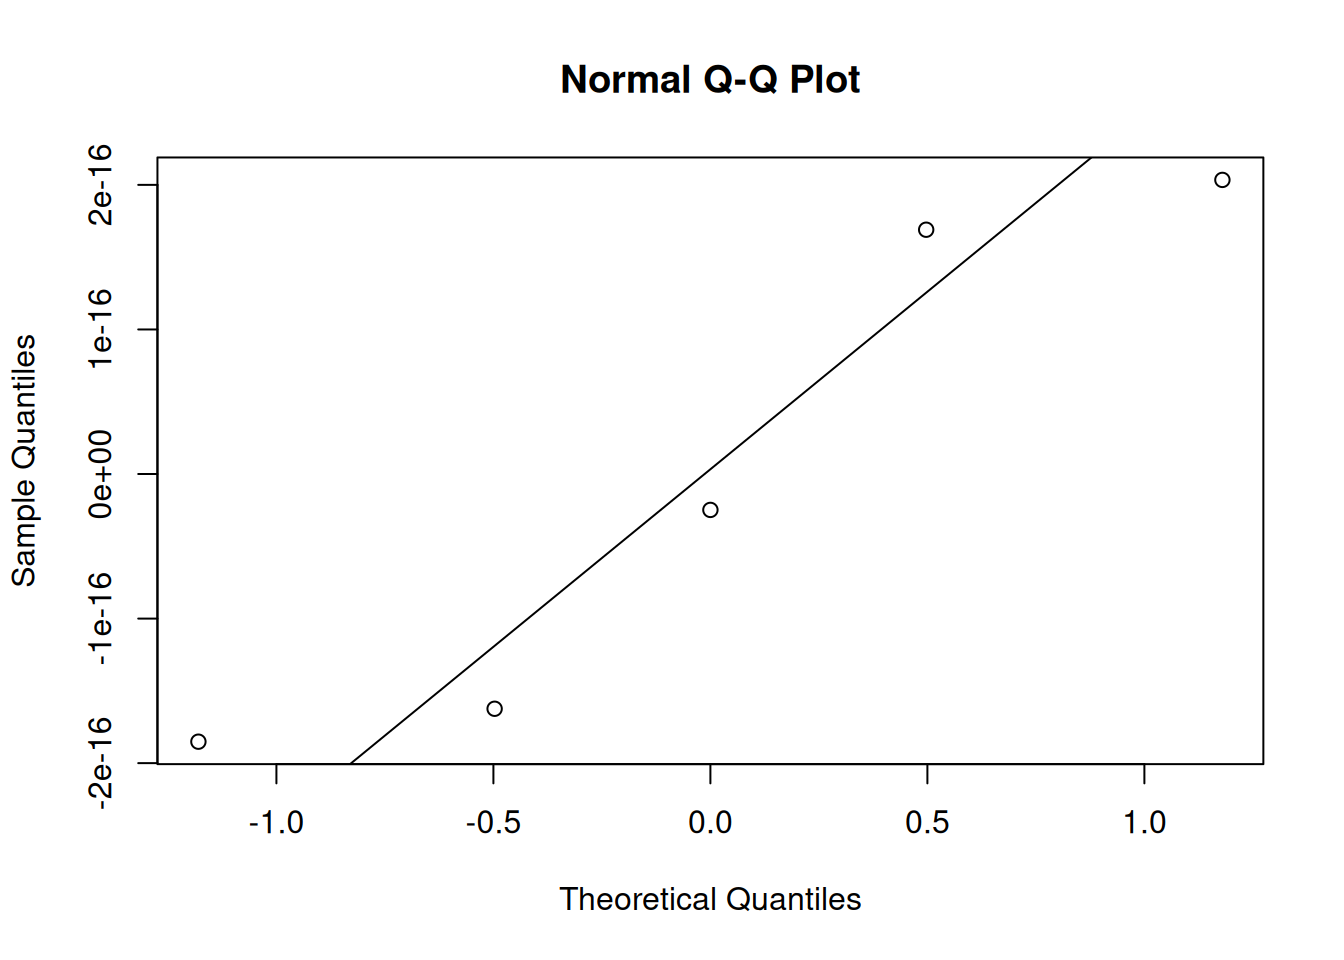
\includegraphics{03-summary_statistics_files/figure-latex/unnamed-chunk-25-2} 

}

\caption{个体生存特征综合分析。左图:生存函数(蓝色)表示生存概率;中图:瞬时死亡风险函数(红色)表示死亡风险率;右图:累积风险函数(深绿色)表示累积死亡风险。}\label{fig:unnamed-chunk-25-2}
\end{figure}

\textbf{生态学意义:}
累积风险函数综合评估个体在整个生命周期中的死亡风险积累,为理解种群生存压力提供整体视角。在保护生物学中,累积风险函数帮助评估濒危物种面临的生存威胁程度;在种群管理中,它为制定保护策略提供量化依据。高累积风险值表明种群面临严重的生存压力,需要采取干预措施。

\hypertarget{ux79cdux7fa4ux7279ux5f81ux63cfux8ff0}{%
\section{种群特征描述}\label{ux79cdux7fa4ux7279ux5f81ux63cfux8ff0}}

种群特征描述关注种群内个体间的资源分配和竞争关系,这些指标在生态学研究中对于理解种群结构、资源利用效率和种内竞争具有重要意义。种群作为生态系统的核心组成单元,其内部个体间的相互作用模式直接影响着种群的动态变化、适应能力和生态系统功能。在资源有限的环境中,个体间不可避免地存在着对光照、水分、养分和空间等关键资源的竞争,这种竞争强度及其导致的资源分配格局是种群生态学研究的核心内容。通过量化种群内个体大小的分布不均等性,我们可以深入理解种内竞争机制、资源捕获策略以及种群对环境变化的响应能力。例如,在森林生态系统中,树木个体对光照的竞争往往导致少数优势个体占据大部分资源,形成典型的层级结构;而在草地生态系统中,相对均等的资源分配可能反映了较为缓和的种内竞争。种群特征描述不仅帮助我们揭示种群的当前状态,还为预测种群未来发展趋势、制定合理的保护管理策略提供了科学依据。在现代生态学研究中,结合数学模型和统计方法对种群特征进行量化分析,已成为理解生物多样性维持机制、生态系统稳定性以及全球变化背景下种群适应性演化的重要途径。

\hypertarget{giniux7cfbux6570}{%
\subsection{Gini系数}\label{giniux7cfbux6570}}

Gini系数是衡量种群内个体大小或资源分配不均等性的重要指标,取值范围在0到1之间,值越大表示分配越不均等。

\textbf{数学定义:}
\[G = \frac{\sum_{i=1}^{n}\sum_{j=1}^{n}|x_i - x_j|}{2n^2\bar{x}}\]

其中:
- \(n\) 为种群个体数量
- \(x_i\) 为第 \(i\) 个个体的生物量或资源量
- \(\bar{x}\) 为个体大小的平均值

\textbf{R代码实现:}

\begin{Shaded}
\begin{Highlighting}[]
\CommentTok{\# 示例数据:森林中树木的胸径(cm)}
\NormalTok{tree\_diameters }\OtherTok{\textless{}{-}} \FunctionTok{c}\NormalTok{(}
  \FloatTok{15.2}\NormalTok{, }\FloatTok{18.5}\NormalTok{, }\FloatTok{22.1}\NormalTok{, }\FloatTok{25.8}\NormalTok{, }\FloatTok{28.3}\NormalTok{, }\FloatTok{32.6}\NormalTok{, }\FloatTok{35.9}\NormalTok{, }\FloatTok{40.2}\NormalTok{,}
  \FloatTok{45.7}\NormalTok{, }\FloatTok{50.3}\NormalTok{, }\FloatTok{12.8}\NormalTok{, }\FloatTok{16.4}\NormalTok{, }\FloatTok{19.7}\NormalTok{, }\FloatTok{23.5}\NormalTok{, }\FloatTok{27.9}
\NormalTok{)}

\CommentTok{\# 计算Gini系数}
\NormalTok{calculate\_gini }\OtherTok{\textless{}{-}} \ControlFlowTok{function}\NormalTok{(x) \{}
\NormalTok{  n }\OtherTok{\textless{}{-}} \FunctionTok{length}\NormalTok{(x)}
\NormalTok{  x\_sorted }\OtherTok{\textless{}{-}} \FunctionTok{sort}\NormalTok{(x)}
\NormalTok{  numerator }\OtherTok{\textless{}{-}} \FunctionTok{sum}\NormalTok{((}\DecValTok{2} \SpecialCharTok{*} \DecValTok{1}\SpecialCharTok{:}\NormalTok{n }\SpecialCharTok{{-}}\NormalTok{ n }\SpecialCharTok{{-}} \DecValTok{1}\NormalTok{) }\SpecialCharTok{*}\NormalTok{ x\_sorted)}
\NormalTok{  denominator }\OtherTok{\textless{}{-}}\NormalTok{ n }\SpecialCharTok{*} \FunctionTok{sum}\NormalTok{(x\_sorted)}
  \FunctionTok{return}\NormalTok{(numerator }\SpecialCharTok{/}\NormalTok{ denominator)}
\NormalTok{\}}

\NormalTok{gini\_index }\OtherTok{\textless{}{-}} \FunctionTok{calculate\_gini}\NormalTok{(tree\_diameters)}

\FunctionTok{cat}\NormalTok{(}\StringTok{"树木胸径的Gini系数:"}\NormalTok{, }\FunctionTok{round}\NormalTok{(gini\_index, }\DecValTok{3}\NormalTok{), }\StringTok{"}\SpecialCharTok{\textbackslash{}n}\StringTok{"}\NormalTok{)}
\end{Highlighting}
\end{Shaded}

\begin{verbatim}
## 树木胸径的Gini系数: 0.222
\end{verbatim}

\begin{Shaded}
\begin{Highlighting}[]
\CommentTok{\# 使用ineq包验证计算结果}
\FunctionTok{library}\NormalTok{(ineq)}
\NormalTok{gini\_ineq }\OtherTok{\textless{}{-}}\NormalTok{ ineq}\SpecialCharTok{::}\FunctionTok{Gini}\NormalTok{(tree\_diameters)}
\FunctionTok{cat}\NormalTok{(}\StringTok{"使用ineq包计算的Gini系数:"}\NormalTok{, }\FunctionTok{round}\NormalTok{(gini\_ineq, }\DecValTok{3}\NormalTok{), }\StringTok{"}\SpecialCharTok{\textbackslash{}n}\StringTok{"}\NormalTok{)}
\end{Highlighting}
\end{Shaded}

\begin{verbatim}
## 使用ineq包计算的Gini系数: 0.222
\end{verbatim}

\begin{Shaded}
\begin{Highlighting}[]
\CommentTok{\# 可视化个体大小分布}
\FunctionTok{library}\NormalTok{(ggplot2)}
\NormalTok{tree\_data }\OtherTok{\textless{}{-}} \FunctionTok{data.frame}\NormalTok{(}\AttributeTok{diameter =}\NormalTok{ tree\_diameters, }\AttributeTok{rank =} \FunctionTok{rank}\NormalTok{(tree\_diameters))}

\FunctionTok{ggplot}\NormalTok{(tree\_data, }\FunctionTok{aes}\NormalTok{(}\AttributeTok{x =}\NormalTok{ rank, }\AttributeTok{y =}\NormalTok{ diameter)) }\SpecialCharTok{+}
  \FunctionTok{geom\_point}\NormalTok{(}\AttributeTok{size =} \DecValTok{3}\NormalTok{, }\AttributeTok{color =} \StringTok{"blue"}\NormalTok{, }\AttributeTok{alpha =} \FloatTok{0.7}\NormalTok{) }\SpecialCharTok{+}
  \FunctionTok{geom\_hline}\NormalTok{(}\AttributeTok{yintercept =} \FunctionTok{mean}\NormalTok{(tree\_diameters),}
             \AttributeTok{linetype =} \StringTok{"dashed"}\NormalTok{, }\AttributeTok{color =} \StringTok{"red"}\NormalTok{) }\SpecialCharTok{+}
  \FunctionTok{labs}\NormalTok{(}
    \AttributeTok{title =} \StringTok{"树木胸径分布"}\NormalTok{,}
    \AttributeTok{subtitle =} \FunctionTok{paste}\NormalTok{(}\StringTok{"Gini系数 ="}\NormalTok{, }\FunctionTok{round}\NormalTok{(gini\_index, }\DecValTok{3}\NormalTok{)),}
    \AttributeTok{x =} \StringTok{"个体排序"}\NormalTok{, }\AttributeTok{y =} \StringTok{"胸径 (cm)"}
\NormalTok{  ) }\SpecialCharTok{+}
  \FunctionTok{theme\_minimal}\NormalTok{()}
\end{Highlighting}
\end{Shaded}

\begin{figure}

{\centering \includegraphics{03-summary_statistics_files/figure-latex/unnamed-chunk-26-1} 

}

\caption{树木胸径分布图。蓝色点表示个体胸径值,红色虚线表示平均胸径,用于计算和可视化Gini系数,反映种群内个体大小的不均等性。}\label{fig:unnamed-chunk-26}
\end{figure}

\textbf{生态学意义:}
Gini系数在生态学中用于描述种群内个体竞争强度和资源分配公平性。例如,在森林生态系统中,高Gini系数表明少数大树占据了大部分资源,反映了强烈的种内竞争;低Gini系数则表明资源分配相对均等,个体间竞争较弱。Gini系数帮助我们理解种群的结构动态和资源利用模式。

\hypertarget{lorenzux66f2ux7ebf}{%
\subsection{Lorenz曲线}\label{lorenzux66f2ux7ebf}}

Lorenz曲线是可视化种群内个体大小分布不均等性的图形工具,通过累积个体大小与累积个体数量的关系曲线来展示资源分配模式。

\textbf{数学定义:}
Lorenz曲线上的点 \((p, L(p))\) 表示:
- \(p\):累积个体比例(从小到大排序)
- \(L(p)\):对应个体累积的资源比例

\textbf{R代码实现:}

\begin{Shaded}
\begin{Highlighting}[]
\CommentTok{\# 计算Lorenz曲线数据}
\NormalTok{calculate\_lorenz }\OtherTok{\textless{}{-}} \ControlFlowTok{function}\NormalTok{(x) \{}
\NormalTok{  x\_sorted }\OtherTok{\textless{}{-}} \FunctionTok{sort}\NormalTok{(x)}
\NormalTok{  n }\OtherTok{\textless{}{-}} \FunctionTok{length}\NormalTok{(x)}
\NormalTok{  p }\OtherTok{\textless{}{-}}\NormalTok{ (}\DecValTok{1}\SpecialCharTok{:}\NormalTok{n) }\SpecialCharTok{/}\NormalTok{ n }\CommentTok{\# 累积个体比例}
\NormalTok{  L }\OtherTok{\textless{}{-}} \FunctionTok{cumsum}\NormalTok{(x\_sorted) }\SpecialCharTok{/} \FunctionTok{sum}\NormalTok{(x\_sorted) }\CommentTok{\# 累积资源比例}
  \FunctionTok{return}\NormalTok{(}\FunctionTok{data.frame}\NormalTok{(}\AttributeTok{p =}\NormalTok{ p, }\AttributeTok{L =}\NormalTok{ L))}
\NormalTok{\}}

\NormalTok{lorenz\_data }\OtherTok{\textless{}{-}} \FunctionTok{calculate\_lorenz}\NormalTok{(tree\_diameters)}

\CommentTok{\# 绘制Lorenz曲线}
\FunctionTok{ggplot}\NormalTok{(lorenz\_data, }\FunctionTok{aes}\NormalTok{(}\AttributeTok{x =}\NormalTok{ p, }\AttributeTok{y =}\NormalTok{ L)) }\SpecialCharTok{+}
  \FunctionTok{geom\_line}\NormalTok{(}\AttributeTok{color =} \StringTok{"darkgreen"}\NormalTok{, }\AttributeTok{size =} \FloatTok{1.5}\NormalTok{) }\SpecialCharTok{+}
  \FunctionTok{geom\_abline}\NormalTok{(}\AttributeTok{intercept =} \DecValTok{0}\NormalTok{, }\AttributeTok{slope =} \DecValTok{1}\NormalTok{, }\AttributeTok{linetype =} \StringTok{"dashed"}\NormalTok{, }\AttributeTok{color =} \StringTok{"gray"}\NormalTok{) }\SpecialCharTok{+}
  \FunctionTok{geom\_polygon}\NormalTok{(}
    \AttributeTok{data =} \FunctionTok{data.frame}\NormalTok{(}\AttributeTok{x =} \FunctionTok{c}\NormalTok{(}\DecValTok{0}\NormalTok{, lorenz\_data}\SpecialCharTok{$}\NormalTok{p, }\DecValTok{1}\NormalTok{), }\AttributeTok{y =} \FunctionTok{c}\NormalTok{(}\DecValTok{0}\NormalTok{, lorenz\_data}\SpecialCharTok{$}\NormalTok{L, }\DecValTok{0}\NormalTok{)),}
    \FunctionTok{aes}\NormalTok{(}\AttributeTok{x =}\NormalTok{ x, }\AttributeTok{y =}\NormalTok{ y), }\AttributeTok{fill =} \StringTok{"lightgreen"}\NormalTok{, }\AttributeTok{alpha =} \FloatTok{0.3}
\NormalTok{  ) }\SpecialCharTok{+}
  \FunctionTok{labs}\NormalTok{(}
    \AttributeTok{title =} \StringTok{"Lorenz曲线"}\NormalTok{,}
    \AttributeTok{subtitle =} \FunctionTok{paste}\NormalTok{(}\StringTok{"Gini系数 ="}\NormalTok{, }\FunctionTok{round}\NormalTok{(gini\_index, }\DecValTok{3}\NormalTok{)),}
    \AttributeTok{x =} \StringTok{"累积个体比例"}\NormalTok{, }\AttributeTok{y =} \StringTok{"累积资源比例"}
\NormalTok{  ) }\SpecialCharTok{+}
  \FunctionTok{theme\_minimal}\NormalTok{() }\SpecialCharTok{+}
  \FunctionTok{coord\_equal}\NormalTok{()}
\end{Highlighting}
\end{Shaded}

\begin{figure}

{\centering \includegraphics{03-summary_statistics_files/figure-latex/unnamed-chunk-27-1} 

}

\caption{Lorenz曲线图。深绿色曲线表示累积资源分配比例,灰色对角线表示完全均等分配,浅绿色区域表示基尼面积,用于可视化种群内资源分配的不均等性。}\label{fig:unnamed-chunk-27}
\end{figure}

\begin{Shaded}
\begin{Highlighting}[]
\CommentTok{\# 计算基尼面积(Lorenz曲线与对角线之间的面积)}
\NormalTok{gini\_area }\OtherTok{\textless{}{-}} \FloatTok{0.5} \SpecialCharTok{{-}} \FunctionTok{sum}\NormalTok{(}\FunctionTok{diff}\NormalTok{(lorenz\_data}\SpecialCharTok{$}\NormalTok{p) }\SpecialCharTok{*}
\NormalTok{                         (lorenz\_data}\SpecialCharTok{$}\NormalTok{L[}\SpecialCharTok{{-}}\DecValTok{1}\NormalTok{] }\SpecialCharTok{+}
\NormalTok{                            lorenz\_data}\SpecialCharTok{$}\NormalTok{L[}\SpecialCharTok{{-}}\FunctionTok{nrow}\NormalTok{(lorenz\_data)])) }\SpecialCharTok{/} \DecValTok{2}
\FunctionTok{cat}\NormalTok{(}\StringTok{"基尼面积:"}\NormalTok{, }\FunctionTok{round}\NormalTok{(gini\_area, }\DecValTok{4}\NormalTok{), }\StringTok{"}\SpecialCharTok{\textbackslash{}n}\StringTok{"}\NormalTok{)}
\end{Highlighting}
\end{Shaded}

\begin{verbatim}
## 基尼面积: 0.1118
\end{verbatim}

\textbf{生态学意义:}
Lorenz曲线直观地展示了种群内资源分配的不均等性。曲线越接近对角线,资源分配越均等;曲线越向下弯曲,资源分配越不均等。在生态学研究中,Lorenz曲线帮助我们可视化种内竞争格局,理解优势个体对资源的控制程度。

\hypertarget{ux57faux5c3cux7cfbux6570ux7684ux751fux6001ux5b66ux5e94ux7528}{%
\subsection{基尼系数的生态学应用}\label{ux57faux5c3cux7cfbux6570ux7684ux751fux6001ux5b66ux5e94ux7528}}

基尼系数在生态学研究中具有广泛的应用价值,主要体现在以下几个方面:

\textbf{评估种内竞争强度:}

\begin{Shaded}
\begin{Highlighting}[]
\CommentTok{\# 比较不同种群的竞争强度}
\NormalTok{population\_a }\OtherTok{\textless{}{-}} \FunctionTok{c}\NormalTok{(}\DecValTok{12}\NormalTok{, }\DecValTok{15}\NormalTok{, }\DecValTok{18}\NormalTok{, }\DecValTok{22}\NormalTok{, }\DecValTok{25}\NormalTok{, }\DecValTok{28}\NormalTok{, }\DecValTok{32}\NormalTok{, }\DecValTok{35}\NormalTok{, }\DecValTok{40}\NormalTok{, }\DecValTok{45}\NormalTok{) }\CommentTok{\# 竞争较弱}
\NormalTok{population\_b }\OtherTok{\textless{}{-}} \FunctionTok{c}\NormalTok{(}\DecValTok{8}\NormalTok{, }\DecValTok{10}\NormalTok{, }\DecValTok{12}\NormalTok{, }\DecValTok{15}\NormalTok{, }\DecValTok{20}\NormalTok{, }\DecValTok{30}\NormalTok{, }\DecValTok{42}\NormalTok{, }\DecValTok{55}\NormalTok{, }\DecValTok{68}\NormalTok{, }\DecValTok{80}\NormalTok{) }\CommentTok{\# 竞争较强}

\NormalTok{gini\_a }\OtherTok{\textless{}{-}} \FunctionTok{calculate\_gini}\NormalTok{(population\_a)}
\NormalTok{gini\_b }\OtherTok{\textless{}{-}} \FunctionTok{calculate\_gini}\NormalTok{(population\_b)}

\FunctionTok{cat}\NormalTok{(}\StringTok{"种群A的Gini系数:"}\NormalTok{, }\FunctionTok{round}\NormalTok{(gini\_a, }\DecValTok{3}\NormalTok{), }\StringTok{"(竞争较弱)}\SpecialCharTok{\textbackslash{}n}\StringTok{"}\NormalTok{)}
\end{Highlighting}
\end{Shaded}

\begin{verbatim}
## 种群A的Gini系数: 0.217 (竞争较弱)
\end{verbatim}

\begin{Shaded}
\begin{Highlighting}[]
\FunctionTok{cat}\NormalTok{(}\StringTok{"种群B的Gini系数:"}\NormalTok{, }\FunctionTok{round}\NormalTok{(gini\_b, }\DecValTok{3}\NormalTok{), }\StringTok{"(竞争较强)}\SpecialCharTok{\textbackslash{}n}\StringTok{"}\NormalTok{)}
\end{Highlighting}
\end{Shaded}

\begin{verbatim}
## 种群B的Gini系数: 0.4 (竞争较强)
\end{verbatim}

\begin{Shaded}
\begin{Highlighting}[]
\CommentTok{\# 可视化比较}
\NormalTok{comparison\_data }\OtherTok{\textless{}{-}} \FunctionTok{rbind}\NormalTok{(}
  \FunctionTok{data.frame}\NormalTok{(}\AttributeTok{population =} \StringTok{"A"}\NormalTok{, }\AttributeTok{value =}\NormalTok{ population\_a),}
  \FunctionTok{data.frame}\NormalTok{(}\AttributeTok{population =} \StringTok{"B"}\NormalTok{, }\AttributeTok{value =}\NormalTok{ population\_b)}
\NormalTok{)}

\FunctionTok{ggplot}\NormalTok{(comparison\_data, }\FunctionTok{aes}\NormalTok{(}\AttributeTok{x =}\NormalTok{ population, }\AttributeTok{y =}\NormalTok{ value, }\AttributeTok{fill =}\NormalTok{ population)) }\SpecialCharTok{+}
  \FunctionTok{geom\_boxplot}\NormalTok{(}\AttributeTok{alpha =} \FloatTok{0.7}\NormalTok{) }\SpecialCharTok{+}
  \FunctionTok{geom\_jitter}\NormalTok{(}\AttributeTok{width =} \FloatTok{0.2}\NormalTok{, }\AttributeTok{size =} \DecValTok{2}\NormalTok{, }\AttributeTok{alpha =} \FloatTok{0.6}\NormalTok{) }\SpecialCharTok{+}
  \FunctionTok{labs}\NormalTok{(}
    \AttributeTok{title =} \StringTok{"不同种群的个体大小分布比较"}\NormalTok{,}
    \AttributeTok{subtitle =} \FunctionTok{paste}\NormalTok{(}\StringTok{"Gini系数: A ="}\NormalTok{, }\FunctionTok{round}\NormalTok{(gini\_a, }\DecValTok{3}\NormalTok{),}
                     \StringTok{", B ="}\NormalTok{, }\FunctionTok{round}\NormalTok{(gini\_b, }\DecValTok{3}\NormalTok{)),}
    \AttributeTok{x =} \StringTok{"种群"}\NormalTok{, }\AttributeTok{y =} \StringTok{"个体大小"}
\NormalTok{  ) }\SpecialCharTok{+}
  \FunctionTok{theme\_minimal}\NormalTok{()}
\end{Highlighting}
\end{Shaded}

\begin{figure}

{\centering \includegraphics{03-summary_statistics_files/figure-latex/unnamed-chunk-28-1} 

}

\caption{不同种群的个体大小分布比较。通过箱线图和散点图展示竞争强度不同的两个种群的个体大小分布,用于比较Gini系数和种内竞争格局。}\label{fig:unnamed-chunk-28}
\end{figure}

\textbf{分析资源利用效率:}
高Gini系数的种群通常表明资源集中在少数个体手中,这可能反映了高效的资源捕获能力,但也可能导致种群稳定性下降。通过监测Gini系数的变化,可以评估种群对环境的适应性和资源利用策略的演化。

\textbf{比较不同种群的个体大小分布模式:}

\begin{Shaded}
\begin{Highlighting}[]
\CommentTok{\# 模拟不同环境条件下的种群分布}
\FunctionTok{set.seed}\NormalTok{(}\DecValTok{123}\NormalTok{)}
\NormalTok{resource\_rich }\OtherTok{\textless{}{-}} \FunctionTok{rnorm}\NormalTok{(}\DecValTok{50}\NormalTok{, }\AttributeTok{mean =} \DecValTok{30}\NormalTok{, }\AttributeTok{sd =} \DecValTok{5}\NormalTok{) }\CommentTok{\# 资源丰富环境}
\NormalTok{resource\_poor }\OtherTok{\textless{}{-}} \FunctionTok{rnorm}\NormalTok{(}\DecValTok{50}\NormalTok{, }\AttributeTok{mean =} \DecValTok{20}\NormalTok{, }\AttributeTok{sd =} \DecValTok{8}\NormalTok{) }\CommentTok{\# 资源贫乏环境}

\NormalTok{gini\_rich }\OtherTok{\textless{}{-}} \FunctionTok{calculate\_gini}\NormalTok{(resource\_rich)}
\NormalTok{gini\_poor }\OtherTok{\textless{}{-}} \FunctionTok{calculate\_gini}\NormalTok{(resource\_poor)}

\FunctionTok{cat}\NormalTok{(}\StringTok{"资源丰富环境的Gini系数:"}\NormalTok{, }\FunctionTok{round}\NormalTok{(gini\_rich, }\DecValTok{3}\NormalTok{), }\StringTok{"}\SpecialCharTok{\textbackslash{}n}\StringTok{"}\NormalTok{)}
\end{Highlighting}
\end{Shaded}

\begin{verbatim}
## 资源丰富环境的Gini系数: 0.086
\end{verbatim}

\begin{Shaded}
\begin{Highlighting}[]
\FunctionTok{cat}\NormalTok{(}\StringTok{"资源贫乏环境的Gini系数:"}\NormalTok{, }\FunctionTok{round}\NormalTok{(gini\_poor, }\DecValTok{3}\NormalTok{), }\StringTok{"}\SpecialCharTok{\textbackslash{}n}\StringTok{"}\NormalTok{)}
\end{Highlighting}
\end{Shaded}

\begin{verbatim}
## 资源贫乏环境的Gini系数: 0.189
\end{verbatim}

\begin{Shaded}
\begin{Highlighting}[]
\CommentTok{\# 综合分析}
\NormalTok{efficiency\_analysis }\OtherTok{\textless{}{-}} \FunctionTok{data.frame}\NormalTok{(}
\NormalTok{  环境条件 }\OtherTok{=} \FunctionTok{c}\NormalTok{(}\StringTok{"资源丰富"}\NormalTok{, }\StringTok{"资源贫乏"}\NormalTok{),}
\NormalTok{  Gini系数 }\OtherTok{=} \FunctionTok{c}\NormalTok{(gini\_rich, gini\_poor),}
\NormalTok{  平均大小 }\OtherTok{=} \FunctionTok{c}\NormalTok{(}\FunctionTok{mean}\NormalTok{(resource\_rich), }\FunctionTok{mean}\NormalTok{(resource\_poor)),}
\NormalTok{  变异系数 }\OtherTok{=} \FunctionTok{c}\NormalTok{(}
    \FunctionTok{sd}\NormalTok{(resource\_rich) }\SpecialCharTok{/} \FunctionTok{mean}\NormalTok{(resource\_rich),}
    \FunctionTok{sd}\NormalTok{(resource\_poor) }\SpecialCharTok{/} \FunctionTok{mean}\NormalTok{(resource\_poor)}
\NormalTok{  )}
\NormalTok{)}

\FunctionTok{print}\NormalTok{(}\StringTok{"不同环境条件下的种群特征比较:"}\NormalTok{)}
\end{Highlighting}
\end{Shaded}

\begin{verbatim}
## [1] "不同环境条件下的种群特征比较:"
\end{verbatim}

\begin{Shaded}
\begin{Highlighting}[]
\FunctionTok{print}\NormalTok{(efficiency\_analysis)}
\end{Highlighting}
\end{Shaded}

\begin{verbatim}
##   环境条件   Gini系数 平均大小  变异系数
## 1 资源丰富 0.08611673 30.17202 0.1534319
## 2 资源贫乏 0.18922016 21.17127 0.3421419
\end{verbatim}

\textbf{生态学意义总结:}
基尼系数和Lorenz曲线为生态学家提供了量化种群内资源分配不均等性的工具。这些指标不仅帮助我们理解种内竞争机制,还为种群管理、保护生物学和生态系统功能研究提供了重要依据。通过分析不同环境条件下Gini系数的变化,我们可以深入理解种群对环境变化的响应策略和适应性演化。

\hypertarget{ux7fa4ux843dux7279ux5f81ux63cfux8ff0}{%
\section{群落特征描述}\label{ux7fa4ux843dux7279ux5f81ux63cfux8ff0}}

\hypertarget{ux7269ux79cdux591aux6837ux6027ux63cfux8ff0}{%
\subsection{物种多样性描述}\label{ux7269ux79cdux591aux6837ux6027ux63cfux8ff0}}

物种多样性是生态学研究的核心内容之一,它描述了生物群落在物种组成、数量分布和生态功能等方面的复杂程度。物种多样性不仅反映了生态系统的稳定性和恢复力,还为理解生物进化、群落构建机制和生态系统功能提供了重要依据。

\hypertarget{fishers-ux3b1}{%
\subsubsection{Fisher's α}\label{fishers-ux3b1}}

Fisher's α是基于对数级数分布的物种多样性度量方法,它在样本量变化时相对稳定,特别适用于比较不同采样强度的群落。

\textbf{数学定义:}
Fisher's α 通过对数级数分布拟合得到:
\[S = \alpha \ln(1 + \frac{N}{\alpha})\]

其中:
- \(S\) 为观测到的物种数
- \(N\) 为总个体数
- \(\alpha\) 为Fisher's α 多样性指数

\textbf{R代码实现:}

\begin{Shaded}
\begin{Highlighting}[]
\CommentTok{\# 示例数据:森林群落中不同树种的个体数量}
\NormalTok{species\_abundance }\OtherTok{\textless{}{-}} \FunctionTok{c}\NormalTok{(}\DecValTok{25}\NormalTok{, }\DecValTok{18}\NormalTok{, }\DecValTok{12}\NormalTok{, }\DecValTok{8}\NormalTok{, }\DecValTok{5}\NormalTok{) }\CommentTok{\# 各树种的个体数量}

\CommentTok{\# 计算Fisher\textquotesingle{}s α}
\NormalTok{calculate\_fisher\_alpha }\OtherTok{\textless{}{-}} \ControlFlowTok{function}\NormalTok{(abundance) \{}
\NormalTok{  S }\OtherTok{\textless{}{-}} \FunctionTok{length}\NormalTok{(abundance) }\CommentTok{\# 物种数}
\NormalTok{  N }\OtherTok{\textless{}{-}} \FunctionTok{sum}\NormalTok{(abundance) }\CommentTok{\# 总个体数}

  \CommentTok{\# 使用迭代法求解Fisher\textquotesingle{}s α}
\NormalTok{  alpha\_est }\OtherTok{\textless{}{-}} \DecValTok{1}
  \ControlFlowTok{for}\NormalTok{ (i }\ControlFlowTok{in} \DecValTok{1}\SpecialCharTok{:}\DecValTok{20}\NormalTok{) \{}
\NormalTok{    f }\OtherTok{\textless{}{-}}\NormalTok{ S }\SpecialCharTok{{-}}\NormalTok{ alpha\_est }\SpecialCharTok{*} \FunctionTok{log}\NormalTok{(}\DecValTok{1} \SpecialCharTok{+}\NormalTok{ N }\SpecialCharTok{/}\NormalTok{ alpha\_est)}
\NormalTok{    df }\OtherTok{\textless{}{-}} \SpecialCharTok{{-}}\FunctionTok{log}\NormalTok{(}\DecValTok{1} \SpecialCharTok{+}\NormalTok{ N }\SpecialCharTok{/}\NormalTok{ alpha\_est) }\SpecialCharTok{+}
\NormalTok{      alpha\_est }\SpecialCharTok{*}\NormalTok{ (N }\SpecialCharTok{/}\NormalTok{ (alpha\_est}\SpecialCharTok{\^{}}\DecValTok{2} \SpecialCharTok{+}\NormalTok{ alpha\_est }\SpecialCharTok{*}\NormalTok{ N))}
\NormalTok{    alpha\_est }\OtherTok{\textless{}{-}}\NormalTok{ alpha\_est }\SpecialCharTok{{-}}\NormalTok{ f }\SpecialCharTok{/}\NormalTok{ df}
\NormalTok{  \}}
  \FunctionTok{return}\NormalTok{(alpha\_est)}
\NormalTok{\}}

\NormalTok{fisher\_alpha }\OtherTok{\textless{}{-}} \FunctionTok{calculate\_fisher\_alpha}\NormalTok{(species\_abundance)}

\FunctionTok{cat}\NormalTok{(}\StringTok{"Fisher\textquotesingle{}s α:"}\NormalTok{, }\FunctionTok{round}\NormalTok{(fisher\_alpha, }\DecValTok{3}\NormalTok{), }\StringTok{"}\SpecialCharTok{\textbackslash{}n}\StringTok{"}\NormalTok{)}
\end{Highlighting}
\end{Shaded}

\begin{verbatim}
## Fisher's α: 1.244
\end{verbatim}

\begin{Shaded}
\begin{Highlighting}[]
\CommentTok{\# 使用vegan包验证计算结果}
\NormalTok{fisher\_vegan }\OtherTok{\textless{}{-}}\NormalTok{ vegan}\SpecialCharTok{::}\FunctionTok{fisher.alpha}\NormalTok{(species\_abundance)}
\FunctionTok{cat}\NormalTok{(}\StringTok{"使用vegan包计算的Fisher\textquotesingle{}s α:"}\NormalTok{, }\FunctionTok{round}\NormalTok{(fisher\_vegan, }\DecValTok{3}\NormalTok{), }\StringTok{"}\SpecialCharTok{\textbackslash{}n}\StringTok{"}\NormalTok{)}
\end{Highlighting}
\end{Shaded}

\begin{verbatim}
## 使用vegan包计算的Fisher's α: 1.244
\end{verbatim}

\begin{Shaded}
\begin{Highlighting}[]
\CommentTok{\# 计算Shannon{-}Wiener指数(用于比较)}
\NormalTok{calculate\_shannon }\OtherTok{\textless{}{-}} \ControlFlowTok{function}\NormalTok{(abundance) \{}
\NormalTok{  total }\OtherTok{\textless{}{-}} \FunctionTok{sum}\NormalTok{(abundance)}
\NormalTok{  p }\OtherTok{\textless{}{-}}\NormalTok{ abundance }\SpecialCharTok{/}\NormalTok{ total}
\NormalTok{  H }\OtherTok{\textless{}{-}} \SpecialCharTok{{-}}\FunctionTok{sum}\NormalTok{(p }\SpecialCharTok{*} \FunctionTok{log}\NormalTok{(p))}
  \FunctionTok{return}\NormalTok{(H)}
\NormalTok{\}}

\CommentTok{\# 分析样本量对多样性的影响}
\NormalTok{sample\_sizes }\OtherTok{\textless{}{-}} \FunctionTok{c}\NormalTok{(}\DecValTok{50}\NormalTok{, }\DecValTok{100}\NormalTok{, }\DecValTok{200}\NormalTok{, }\DecValTok{500}\NormalTok{)}
\NormalTok{diversity\_comparison }\OtherTok{\textless{}{-}} \FunctionTok{data.frame}\NormalTok{(}
\NormalTok{  样本量 }\OtherTok{=}\NormalTok{ sample\_sizes,}
\NormalTok{  Shannon指数 }\OtherTok{=} \FunctionTok{numeric}\NormalTok{(}\FunctionTok{length}\NormalTok{(sample\_sizes)),}
  \AttributeTok{Fisher\_alpha =} \FunctionTok{numeric}\NormalTok{(}\FunctionTok{length}\NormalTok{(sample\_sizes))}
\NormalTok{)}

\ControlFlowTok{for}\NormalTok{ (i }\ControlFlowTok{in} \FunctionTok{seq\_along}\NormalTok{(sample\_sizes)) \{}
  \CommentTok{\# 模拟不同样本量的群落数据}
\NormalTok{  simulated\_abundance }\OtherTok{\textless{}{-}} \FunctionTok{rpois}\NormalTok{(}\DecValTok{10}\NormalTok{, }\AttributeTok{lambda =}\NormalTok{ sample\_sizes[i] }\SpecialCharTok{/} \DecValTok{10}\NormalTok{)}
\NormalTok{  diversity\_comparison}\SpecialCharTok{$}\NormalTok{Shannon指数[i] }\OtherTok{\textless{}{-}}
    \FunctionTok{calculate\_shannon}\NormalTok{(simulated\_abundance)}
\NormalTok{  diversity\_comparison}\SpecialCharTok{$}\NormalTok{Fisher\_alpha[i] }\OtherTok{\textless{}{-}}
    \FunctionTok{calculate\_fisher\_alpha}\NormalTok{(simulated\_abundance)}
\NormalTok{\}}

\FunctionTok{print}\NormalTok{(}\StringTok{"样本量对多样性指数的影响:"}\NormalTok{)}
\end{Highlighting}
\end{Shaded}

\begin{verbatim}
## [1] "样本量对多样性指数的影响:"
\end{verbatim}

\begin{Shaded}
\begin{Highlighting}[]
\FunctionTok{print}\NormalTok{(diversity\_comparison)}
\end{Highlighting}
\end{Shaded}

\begin{verbatim}
##   样本量 Shannon指数 Fisher_alpha
## 1     50    2.224785     3.843383
## 2    100    2.276299     2.681482
## 3    200    2.279418     2.215373
## 4    500    2.293935     1.758383
\end{verbatim}

\textbf{生态学意义:}
Fisher's α在生态学研究中特别适用于比较不同采样强度或样本量的群落。由于其相对稳定性,Fisher's α能够减少采样偏差对多样性评估的影响,为跨研究比较提供可靠依据。在生物多样性监测和保护区评估中,Fisher's α是重要的参考指标。

\hypertarget{shannon-wienerux6307ux6570}{%
\subsubsection{Shannon-Wiener指数}\label{shannon-wienerux6307ux6570}}

Shannon-Wiener指数是基于信息熵概念的物种多样性度量方法,它综合反映了物种丰富度和均匀度,对稀有物种较为敏感。

\textbf{数学定义:}
\[H' = -\sum_{i=1}^{S} p_i \ln(p_i)\]

其中:
- \(S\) 为物种总数
- \(p_i\) 为第 \(i\) 个物种的相对多度

\textbf{R代码实现:}

\begin{Shaded}
\begin{Highlighting}[]
\CommentTok{\# 示例数据:森林群落中不同树种的个体数量}
\NormalTok{tree\_species }\OtherTok{\textless{}{-}} \FunctionTok{c}\NormalTok{(}\StringTok{"橡树"}\NormalTok{, }\StringTok{"松树"}\NormalTok{, }\StringTok{"枫树"}\NormalTok{, }\StringTok{"桦树"}\NormalTok{, }\StringTok{"杉树"}\NormalTok{)}

\CommentTok{\# 计算Shannon{-}Wiener指数}
\NormalTok{calculate\_shannon }\OtherTok{\textless{}{-}} \ControlFlowTok{function}\NormalTok{(abundance) \{}
\NormalTok{  total }\OtherTok{\textless{}{-}} \FunctionTok{sum}\NormalTok{(abundance)}
\NormalTok{  p }\OtherTok{\textless{}{-}}\NormalTok{ abundance }\SpecialCharTok{/}\NormalTok{ total}
\NormalTok{  H }\OtherTok{\textless{}{-}} \SpecialCharTok{{-}}\FunctionTok{sum}\NormalTok{(p }\SpecialCharTok{*} \FunctionTok{log}\NormalTok{(p))}
  \FunctionTok{return}\NormalTok{(H)}
\NormalTok{\}}

\NormalTok{shannon\_index }\OtherTok{\textless{}{-}} \FunctionTok{calculate\_shannon}\NormalTok{(species\_abundance)}

\FunctionTok{cat}\NormalTok{(}\StringTok{"Shannon{-}Wiener指数:"}\NormalTok{, }\FunctionTok{round}\NormalTok{(shannon\_index, }\DecValTok{3}\NormalTok{), }\StringTok{"}\SpecialCharTok{\textbackslash{}n}\StringTok{"}\NormalTok{)}
\end{Highlighting}
\end{Shaded}

\begin{verbatim}
## Shannon-Wiener指数: 1.47
\end{verbatim}

\begin{Shaded}
\begin{Highlighting}[]
\CommentTok{\# 使用vegan包验证计算结果}
\FunctionTok{library}\NormalTok{(vegan)}
\NormalTok{shannon\_vegan }\OtherTok{\textless{}{-}}\NormalTok{ vegan}\SpecialCharTok{::}\FunctionTok{diversity}\NormalTok{(species\_abundance, }\AttributeTok{index =} \StringTok{"shannon"}\NormalTok{)}
\FunctionTok{cat}\NormalTok{(}\StringTok{"使用vegan包计算的Shannon指数:"}\NormalTok{, }\FunctionTok{round}\NormalTok{(shannon\_vegan, }\DecValTok{3}\NormalTok{), }\StringTok{"}\SpecialCharTok{\textbackslash{}n}\StringTok{"}\NormalTok{)}
\end{Highlighting}
\end{Shaded}

\begin{verbatim}
## 使用vegan包计算的Shannon指数: 1.47
\end{verbatim}

\begin{Shaded}
\begin{Highlighting}[]
\CommentTok{\# 可视化物种组成}
\FunctionTok{library}\NormalTok{(ggplot2)}
\NormalTok{species\_data }\OtherTok{\textless{}{-}} \FunctionTok{data.frame}\NormalTok{(}
  \AttributeTok{species =}\NormalTok{ tree\_species,}
  \AttributeTok{abundance =}\NormalTok{ species\_abundance,}
  \AttributeTok{proportion =}\NormalTok{ species\_abundance }\SpecialCharTok{/} \FunctionTok{sum}\NormalTok{(species\_abundance)}
\NormalTok{)}

\FunctionTok{ggplot}\NormalTok{(species\_data, }\FunctionTok{aes}\NormalTok{(}\AttributeTok{x =}\NormalTok{ species, }\AttributeTok{y =}\NormalTok{ abundance, }\AttributeTok{fill =}\NormalTok{ species)) }\SpecialCharTok{+}
  \FunctionTok{geom\_col}\NormalTok{() }\SpecialCharTok{+}
  \FunctionTok{labs}\NormalTok{(}
    \AttributeTok{title =} \StringTok{"森林群落物种组成"}\NormalTok{,}
    \AttributeTok{subtitle =} \FunctionTok{paste}\NormalTok{(}\StringTok{"Shannon指数 ="}\NormalTok{, }\FunctionTok{round}\NormalTok{(shannon\_index, }\DecValTok{3}\NormalTok{)),}
    \AttributeTok{x =} \StringTok{"树种"}\NormalTok{, }\AttributeTok{y =} \StringTok{"个体数量"}
\NormalTok{  ) }\SpecialCharTok{+}
  \FunctionTok{theme\_minimal}\NormalTok{()}
\end{Highlighting}
\end{Shaded}

\begin{figure}

{\centering 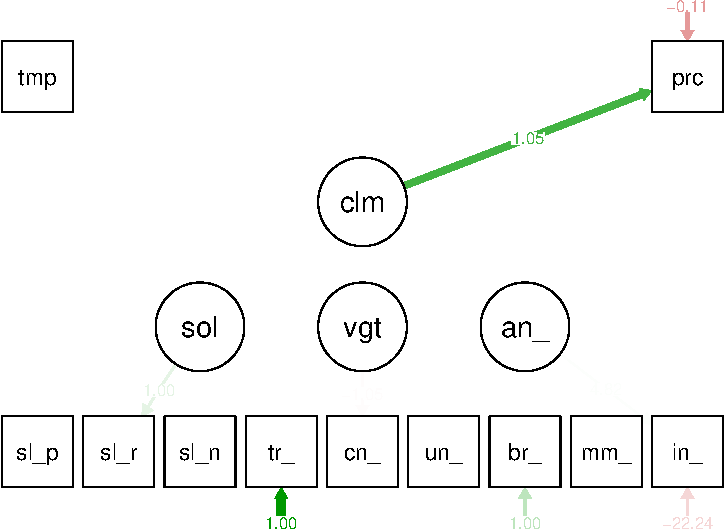
\includegraphics{03-summary_statistics_files/figure-latex/unnamed-chunk-31-1} 

}

\caption{森林群落物种组成柱状图。展示五种树种(橡树、松树、枫树、桦树、杉树)的个体数量分布,用于计算和可视化Shannon-Wiener多样性指数。}\label{fig:unnamed-chunk-31}
\end{figure}

\textbf{生态学意义:}
Shannon-Wiener指数在生态学中广泛应用于评估群落的物种多样性水平。较高的Shannon指数值表明群落具有较高的物种丰富度和均匀度,生态系统通常更加稳定和具有更强的恢复力。该指数对稀有物种较为敏感,能够较好地反映群落的保护价值和生态功能。

\hypertarget{simpsonux6307ux6570}{%
\subsubsection{Simpson指数}\label{simpsonux6307ux6570}}

Simpson指数是基于概率论的物种多样性度量方法,它表示随机抽取两个个体属于不同物种的概率,对优势物种较为敏感。

\textbf{数学定义:}
\[D = 1 - \sum_{i=1}^{S} p_i^2\]

其中:
- \(S\) 为物种总数
- \(p_i\) 为第 \(i\) 个物种的相对多度

\textbf{R代码实现:}

\begin{Shaded}
\begin{Highlighting}[]
\CommentTok{\# 计算Simpson指数}
\NormalTok{calculate\_simpson }\OtherTok{\textless{}{-}} \ControlFlowTok{function}\NormalTok{(abundance) \{}
\NormalTok{  total }\OtherTok{\textless{}{-}} \FunctionTok{sum}\NormalTok{(abundance)}
\NormalTok{  p }\OtherTok{\textless{}{-}}\NormalTok{ abundance }\SpecialCharTok{/}\NormalTok{ total}
\NormalTok{  D }\OtherTok{\textless{}{-}} \DecValTok{1} \SpecialCharTok{{-}} \FunctionTok{sum}\NormalTok{(p}\SpecialCharTok{\^{}}\DecValTok{2}\NormalTok{)}
  \FunctionTok{return}\NormalTok{(D)}
\NormalTok{\}}

\NormalTok{simpson\_index }\OtherTok{\textless{}{-}} \FunctionTok{calculate\_simpson}\NormalTok{(species\_abundance)}

\FunctionTok{cat}\NormalTok{(}\StringTok{"Simpson指数:"}\NormalTok{, }\FunctionTok{round}\NormalTok{(simpson\_index, }\DecValTok{3}\NormalTok{), }\StringTok{"}\SpecialCharTok{\textbackslash{}n}\StringTok{"}\NormalTok{)}
\end{Highlighting}
\end{Shaded}

\begin{verbatim}
## Simpson指数: 0.744
\end{verbatim}

\begin{Shaded}
\begin{Highlighting}[]
\CommentTok{\# 使用vegan包验证计算结果}
\NormalTok{simpson\_vegan }\OtherTok{\textless{}{-}}\NormalTok{ vegan}\SpecialCharTok{::}\FunctionTok{diversity}\NormalTok{(species\_abundance, }\AttributeTok{index =} \StringTok{"simpson"}\NormalTok{)}
\FunctionTok{cat}\NormalTok{(}\StringTok{"使用vegan包计算的Simpson指数:"}\NormalTok{, }\FunctionTok{round}\NormalTok{(simpson\_vegan, }\DecValTok{3}\NormalTok{), }\StringTok{"}\SpecialCharTok{\textbackslash{}n}\StringTok{"}\NormalTok{)}
\end{Highlighting}
\end{Shaded}

\begin{verbatim}
## 使用vegan包计算的Simpson指数: 0.744
\end{verbatim}

\begin{Shaded}
\begin{Highlighting}[]
\CommentTok{\# 比较不同群落的多样性}
\NormalTok{community\_A }\OtherTok{\textless{}{-}} \FunctionTok{c}\NormalTok{(}\DecValTok{30}\NormalTok{, }\DecValTok{25}\NormalTok{, }\DecValTok{20}\NormalTok{, }\DecValTok{15}\NormalTok{, }\DecValTok{10}\NormalTok{) }\CommentTok{\# 多样性较高}
\NormalTok{community\_B }\OtherTok{\textless{}{-}} \FunctionTok{c}\NormalTok{(}\DecValTok{50}\NormalTok{, }\DecValTok{20}\NormalTok{, }\DecValTok{15}\NormalTok{, }\DecValTok{10}\NormalTok{, }\DecValTok{5}\NormalTok{) }\CommentTok{\# 多样性较低}

\NormalTok{shannon\_A }\OtherTok{\textless{}{-}} \FunctionTok{calculate\_shannon}\NormalTok{(community\_A)}
\NormalTok{shannon\_B }\OtherTok{\textless{}{-}} \FunctionTok{calculate\_shannon}\NormalTok{(community\_B)}
\NormalTok{simpson\_A }\OtherTok{\textless{}{-}} \FunctionTok{calculate\_simpson}\NormalTok{(community\_A)}
\NormalTok{simpson\_B }\OtherTok{\textless{}{-}} \FunctionTok{calculate\_simpson}\NormalTok{(community\_B)}

\NormalTok{comparison\_data }\OtherTok{\textless{}{-}} \FunctionTok{data.frame}\NormalTok{(}
\NormalTok{  群落 }\OtherTok{=} \FunctionTok{c}\NormalTok{(}\StringTok{"A"}\NormalTok{, }\StringTok{"B"}\NormalTok{),}
\NormalTok{  Shannon指数 }\OtherTok{=} \FunctionTok{c}\NormalTok{(shannon\_A, shannon\_B),}
\NormalTok{  Simpson指数 }\OtherTok{=} \FunctionTok{c}\NormalTok{(simpson\_A, simpson\_B)}
\NormalTok{)}

\FunctionTok{print}\NormalTok{(}\StringTok{"不同群落的多样性比较:"}\NormalTok{)}
\end{Highlighting}
\end{Shaded}

\begin{verbatim}
## [1] "不同群落的多样性比较:"
\end{verbatim}

\begin{Shaded}
\begin{Highlighting}[]
\FunctionTok{print}\NormalTok{(comparison\_data)}
\end{Highlighting}
\end{Shaded}

\begin{verbatim}
##   群落 Shannon指数 Simpson指数
## 1    A    1.544480       0.775
## 2    B    1.333074       0.675
\end{verbatim}

\textbf{生态学意义:}
Simpson指数特别适用于分析群落中的优势物种格局。较低的Simpson指数值表明群落中存在明显的优势物种,这可能反映了强烈的竞争排斥或环境筛选作用。在生态监测和保护规划中,Simpson指数帮助我们识别需要特别关注的生态关键种和优势种。

\hypertarget{pielouux5747ux5300ux5ea6ux6307ux6570}{%
\subsubsection{Pielou均匀度指数}\label{pielouux5747ux5300ux5ea6ux6307ux6570}}

Pielou均匀度指数是独立于物种丰富度的均匀度度量方法,它反映了物种多度分布的均等程度。

\textbf{数学定义:}
\[J' = \frac{H'}{H'_{max}} = \frac{H'}{\ln(S)}\]

其中:
- \(H'\) 为观测的Shannon指数
- \(H'_{max}\) 为最大可能的Shannon指数(当所有物种多度相等时)
- \(S\) 为物种总数

\textbf{R代码实现:}

\begin{Shaded}
\begin{Highlighting}[]
\CommentTok{\# 计算Pielou均匀度指数}
\NormalTok{calculate\_pielou }\OtherTok{\textless{}{-}} \ControlFlowTok{function}\NormalTok{(abundance) \{}
\NormalTok{  H }\OtherTok{\textless{}{-}} \FunctionTok{calculate\_shannon}\NormalTok{(abundance)}
\NormalTok{  S }\OtherTok{\textless{}{-}} \FunctionTok{length}\NormalTok{(abundance)}
\NormalTok{  J }\OtherTok{\textless{}{-}}\NormalTok{ H }\SpecialCharTok{/} \FunctionTok{log}\NormalTok{(S)}
  \FunctionTok{return}\NormalTok{(J)}
\NormalTok{\}}

\NormalTok{pielou\_index }\OtherTok{\textless{}{-}} \FunctionTok{calculate\_pielou}\NormalTok{(species\_abundance)}

\FunctionTok{cat}\NormalTok{(}\StringTok{"Pielou均匀度指数:"}\NormalTok{, }\FunctionTok{round}\NormalTok{(pielou\_index, }\DecValTok{3}\NormalTok{), }\StringTok{"}\SpecialCharTok{\textbackslash{}n}\StringTok{"}\NormalTok{)}
\end{Highlighting}
\end{Shaded}

\begin{verbatim}
## Pielou均匀度指数: 0.913
\end{verbatim}

\begin{Shaded}
\begin{Highlighting}[]
\CommentTok{\# 比较不同均匀度的群落}
\NormalTok{even\_community }\OtherTok{\textless{}{-}} \FunctionTok{c}\NormalTok{(}\DecValTok{20}\NormalTok{, }\DecValTok{18}\NormalTok{, }\DecValTok{22}\NormalTok{, }\DecValTok{19}\NormalTok{, }\DecValTok{21}\NormalTok{) }\CommentTok{\# 均匀分布}
\NormalTok{uneven\_community }\OtherTok{\textless{}{-}} \FunctionTok{c}\NormalTok{(}\DecValTok{50}\NormalTok{, }\DecValTok{15}\NormalTok{, }\DecValTok{10}\NormalTok{, }\DecValTok{12}\NormalTok{, }\DecValTok{13}\NormalTok{) }\CommentTok{\# 不均匀分布}

\NormalTok{pielou\_even }\OtherTok{\textless{}{-}} \FunctionTok{calculate\_pielou}\NormalTok{(even\_community)}
\NormalTok{pielou\_uneven }\OtherTok{\textless{}{-}} \FunctionTok{calculate\_pielou}\NormalTok{(uneven\_community)}

\CommentTok{\# 可视化均匀度比较}
\NormalTok{uniformity\_data }\OtherTok{\textless{}{-}} \FunctionTok{rbind}\NormalTok{(}
  \FunctionTok{data.frame}\NormalTok{(群落类型 }\OtherTok{=} \StringTok{"均匀分布"}\NormalTok{, 物种 }\OtherTok{=} \DecValTok{1}\SpecialCharTok{:}\DecValTok{5}\NormalTok{, 多度 }\OtherTok{=}\NormalTok{ even\_community),}
  \FunctionTok{data.frame}\NormalTok{(群落类型 }\OtherTok{=} \StringTok{"不均匀分布"}\NormalTok{, 物种 }\OtherTok{=} \DecValTok{1}\SpecialCharTok{:}\DecValTok{5}\NormalTok{, 多度 }\OtherTok{=}\NormalTok{ uneven\_community)}
\NormalTok{)}

\FunctionTok{ggplot}\NormalTok{(uniformity\_data, }\FunctionTok{aes}\NormalTok{(}\AttributeTok{x =} \FunctionTok{factor}\NormalTok{(物种), }\AttributeTok{y =}\NormalTok{ 多度, }\AttributeTok{fill =}\NormalTok{ 群落类型)) }\SpecialCharTok{+}
  \FunctionTok{geom\_col}\NormalTok{(}\AttributeTok{position =} \StringTok{"dodge"}\NormalTok{) }\SpecialCharTok{+}
  \FunctionTok{labs}\NormalTok{(}
    \AttributeTok{title =} \StringTok{"群落均匀度比较"}\NormalTok{,}
    \AttributeTok{subtitle =} \FunctionTok{paste}\NormalTok{(}
      \StringTok{"均匀度指数: 均匀 ="}\NormalTok{, }\FunctionTok{round}\NormalTok{(pielou\_even, }\DecValTok{3}\NormalTok{),}
      \StringTok{", 不均匀 ="}\NormalTok{, }\FunctionTok{round}\NormalTok{(pielou\_uneven, }\DecValTok{3}\NormalTok{)}
\NormalTok{    ),}
    \AttributeTok{x =} \StringTok{"物种"}\NormalTok{, }\AttributeTok{y =} \StringTok{"个体数量"}
\NormalTok{  ) }\SpecialCharTok{+}
  \FunctionTok{theme\_minimal}\NormalTok{() }\SpecialCharTok{+}
  \FunctionTok{facet\_wrap}\NormalTok{(}\SpecialCharTok{\textasciitilde{}}\NormalTok{群落类型, }\AttributeTok{ncol =} \DecValTok{2}\NormalTok{)}
\end{Highlighting}
\end{Shaded}

\begin{center}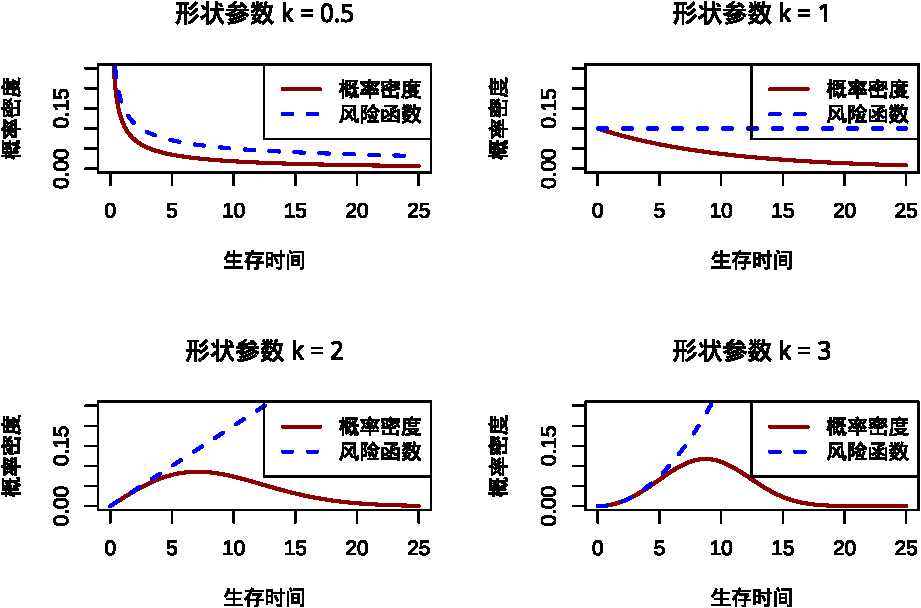
\includegraphics{03-summary_statistics_files/figure-latex/unnamed-chunk-33-1} \end{center}

\begin{Shaded}
\begin{Highlighting}[]
\CommentTok{\# 综合多样性分析}
\NormalTok{diversity\_summary }\OtherTok{\textless{}{-}} \FunctionTok{data.frame}\NormalTok{(}
\NormalTok{  指数类型 }\OtherTok{=} \FunctionTok{c}\NormalTok{(}\StringTok{"Shannon{-}Wiener"}\NormalTok{, }\StringTok{"Simpson"}\NormalTok{, }\StringTok{"Fisher\textquotesingle{}s α"}\NormalTok{, }\StringTok{"Pielou均匀度"}\NormalTok{),}
\NormalTok{  数值 }\OtherTok{=} \FunctionTok{c}\NormalTok{(shannon\_index, simpson\_index, fisher\_alpha, pielou\_index),}
\NormalTok{  解释 }\OtherTok{=} \FunctionTok{c}\NormalTok{(}\StringTok{"综合多样性"}\NormalTok{, }\StringTok{"优势度敏感性"}\NormalTok{, }\StringTok{"样本稳定性"}\NormalTok{, }\StringTok{"均匀度度量"}\NormalTok{)}
\NormalTok{)}

\FunctionTok{print}\NormalTok{(}\StringTok{"群落多样性综合评估:"}\NormalTok{)}
\end{Highlighting}
\end{Shaded}

\begin{verbatim}
## [1] "群落多样性综合评估:"
\end{verbatim}

\begin{Shaded}
\begin{Highlighting}[]
\FunctionTok{print}\NormalTok{(diversity\_summary)}
\end{Highlighting}
\end{Shaded}

\begin{verbatim}
##         指数类型      数值         解释
## 1 Shannon-Wiener 1.4695049   综合多样性
## 2        Simpson 0.7443772 优势度敏感性
## 3     Fisher's α 1.2439951   样本稳定性
## 4   Pielou均匀度 0.9130547   均匀度度量
\end{verbatim}

\textbf{生态学意义:}
Pielou均匀度指数在生态学中用于独立评估物种多度分布的均等程度,不受物种丰富度的影响。高均匀度指数表明群落中资源分配相对均等,种间竞争可能较为缓和;低均匀度指数则反映了明显的优势种格局和强烈的种间竞争。均匀度指数为理解群落构建机制和生态位分化提供了重要信息。

\hypertarget{ux751fux6001ux7f51ux7edcux7279ux5f81ux63cfux8ff0}{%
\section{生态网络特征描述}\label{ux751fux6001ux7f51ux7edcux7279ux5f81ux63cfux8ff0}}

生态网络特征描述关注物种间相互作用的拓扑结构和功能关系,这些指标在生态学研究中对于理解群落稳定性、能量流动和生态系统功能具有重要意义。生态网络分析将生物群落视为复杂的网络系统,其中物种作为节点,它们之间的相互作用作为边,通过图论方法揭示生态系统的组织规律和动态特征。

生态网络分析是现代生态学的重要分支,它将传统的物种-环境关系研究扩展到物种-物种相互作用的网络层面。这种分析方法不仅关注单个物种的生态特征,更注重物种间相互作用的整体格局和结构特征。在生态网络中,每个物种都不是孤立存在的,而是通过捕食、竞争、互利共生等多种关系与其他物种紧密相连,形成一个复杂的相互作用网络。这种网络结构直接影响着生态系统的稳定性、恢复力和功能表现。

生态网络分析的核心在于揭示物种间相互作用的拓扑特征,包括连接度、模块性、嵌套性等关键指标。连接度反映了网络中物种间相互作用的密集程度,高连接度通常意味着更强的功能冗余和系统稳定性;模块性描述了网络内部群落结构的明显程度,高模块性表明系统可以划分为相对独立的子群落,这有助于缓冲局部干扰对整个系统的影响;嵌套性则揭示了特化物种与泛化物种的连接模式,高嵌套性表明系统具有层级结构,特化物种的生存依赖于泛化物种的存在。

在食物网分析中,生态网络特征描述进一步扩展到能量流动和营养关系的结构特征。食物链长度反映了能量在生态系统中的传递效率,较长的食物链通常意味着更高的能量利用效率,但也可能增加系统的不稳定性;连接复杂性则衡量了物种间捕食关系的密集程度,较高的连接复杂性与更强的系统稳定性和功能冗余相关。通过分析这些特征,我们可以深入理解生态系统中能量流动的路径、营养级的构成以及物种间的营养关系。

生态网络分析的应用范围十分广泛,涵盖了植物-传粉者网络、宿主-寄生者网络、竞争网络等多种生态相互作用类型。例如,在植物-传粉者网络中,网络结构特征直接影响着植物的繁殖成功率和传粉者的资源获取;在食物网中,网络拓扑特征决定了能量流动的效率和系统的稳定性。这些网络特征不仅反映了当前的生态状态,还能够预测生态系统对环境变化的响应和适应能力。

随着计算生态学的发展,生态网络分析的方法和技术不断进步。现代生态网络研究结合了图论、复杂系统理论和统计物理学等多个学科的理论和方法,为理解生态系统的复杂性和动态性提供了强有力的工具。通过量化分析生态网络的结构特征,我们可以更好地预测生物多样性的维持机制、生态系统的稳定性阈值以及对全球变化的响应模式。

在保护生物学和生态系统管理中,生态网络特征描述具有重要的实践价值。通过识别网络中的关键物种和脆弱环节,我们可以制定更有针对性的保护策略;通过分析网络结构的变化,我们可以监测生态系统的健康状况和恢复进程。生态网络分析为生物多样性保护、生态系统修复和可持续发展提供了科学依据,是现代生态学研究不可或缺的重要组成部分。

\hypertarget{ux7f51ux7edcux62d3ux6251ux6307ux6807}{%
\subsection{网络拓扑指标}\label{ux7f51ux7edcux62d3ux6251ux6307ux6807}}

网络拓扑指标描述了生态网络的结构特征,包括连接模式、模块组织和嵌套格局等,这些特征直接影响生态系统的稳定性和功能。网络拓扑分析是生态网络研究的核心内容,它通过量化网络的结构特征来揭示物种间相互作用的组织规律和生态系统的功能特性。拓扑指标不仅反映了当前的生态状态,还能够预测生态系统对环境变化的响应能力和恢复潜力。

\textbf{连接度(Connectance):}
连接度是生态网络分析中最基础的拓扑指标之一,它衡量网络中实际连接数与可能连接数的比例,反映了物种间相互作用的密集程度。连接度的取值范围在0到1之间,值越大表明网络中物种间的相互作用越密集。

\textbf{数学定义:}
\[C = \frac{L}{S(S-1)}\]

其中:
- \(L\) 为网络中实际存在的连接数
- \(S\) 为物种总数

连接度的生态学意义十分深远。高连接度通常意味着生态系统具有更强的功能冗余和系统稳定性。在这种网络中,物种间存在大量的相互作用关系,当一个物种消失或数量减少时,其他物种可以通过替代性的相互作用来维持生态系统的功能。例如,在植物-传粉者网络中,高连接度表明传粉者具有多样化的食物来源,植物也具有多样化的传粉者,这种冗余性增强了系统对物种丧失的抵抗能力。然而,过高的连接度也可能带来负面影响,如增加疾病传播的风险或强化种间竞争。连接度的研究帮助我们理解生态系统的复杂性和稳定性之间的平衡关系。

\textbf{模块性(Modularity):}
模块性是衡量网络中群落结构明显程度的重要指标,它量化了网络可以划分为相对独立子群落的能力。高模块性表明网络中存在明显的模块结构,物种在模块内部的相互作用强度远大于模块之间的相互作用。

\textbf{数学定义:}
\[Q = \frac{1}{2m} \sum_{ij} \left[ A_{ij} - \frac{k_i k_j}{2m} \right] \delta(c_i, c_j)\]

其中:
- \(A_{ij}\) 为邻接矩阵元素
- \(k_i\) 为节点 \(i\) 的度
- \(m\) 为总连接数
- \(\delta(c_i, c_j)\) 为节点所属模块指示函数

模块性在生态学中具有重要的功能意义。高模块性的生态系统通常具有较强的抗干扰能力,因为局部的干扰可以被限制在特定的模块内,而不会迅速扩散到整个网络。例如,在珊瑚礁生态系统中,不同的珊瑚礁斑块可能形成相对独立的模块,当一个斑块受到环境压力时,其他斑块可以维持正常的生态功能。模块性还反映了生态位的分化和资源利用的专业化程度。在高度模块化的网络中,物种往往在特定的生态位中特化,形成相对独立的生态功能单元。模块性分析为理解生态系统的空间结构和功能分区提供了重要工具。

\textbf{嵌套性(Nestedness):}
嵌套性是描述特化物种与泛化物种连接模式的关键指标,它反映了网络中物种相互作用的层级结构。高嵌套性表明特化物种的相互作用伙伴是泛化物种相互作用伙伴的子集,形成一种''俄罗斯套娃''式的结构模式。

\textbf{数学定义:}
最常用的嵌套性度量是NODF(Nestedness metric based on Overlap and Decreasing Fill),其数学定义为:

对于行嵌套(物种作为行):
\[NODF_{rows} = \frac{2}{S(S-1)} \sum_{i<j} \frac{O_{ij}}{\min(k_i, k_j)}\]

对于列嵌套(物种作为列):
\[NODF_{cols} = \frac{2}{T(T-1)} \sum_{i<j} \frac{O_{ij}}{\min(k_i, k_j)}\]

总体嵌套性:
\[NODF = \frac{NODF_{rows} + NODF_{cols}}{2}\]

其中:
- \(S\) 为行物种数(如植物)
- \(T\) 为列物种数(如传粉者)
- \(O_{ij}\) 为物种对 \(i\) 和 \(j\) 的共同相互作用数
- \(k_i, k_j\) 为物种 \(i\) 和 \(j\) 的度(相互作用数)

另一种常用的嵌套性度量是温度度量(Temperature metric),基于完美嵌套矩阵与实际矩阵的差异:
\[T = \frac{\sum_{i,j} |a_{ij} - p_{ij}|}{S \times T}\]

其中:
- \(a_{ij}\) 为实际相互作用矩阵
- \(p_{ij}\) 为完美嵌套矩阵

嵌套性的生态学意义在于它揭示了物种共存和资源利用的策略。在高度嵌套的网络中,泛化物种与许多其他物种相互作用,而特化物种只与部分泛化物种相互作用。这种结构模式有助于维持生态系统的稳定性,因为泛化物种可以作为''枢纽''物种,连接不同的功能单元。当环境发生变化时,泛化物种能够维持基本的生态功能,为特化物种提供生存基础。嵌套性结构还反映了生态位分化的程度和物种间相互作用的组织规律。

嵌套性的计算方法有多种,其中最常用的是NODF(Nestedness metric based on Overlap and Decreasing Fill)方法。NODF通过比较物种对的相互作用模式来量化网络的嵌套程度,考虑了行嵌套和列嵌套两个维度。高NODF值表明网络具有明显的嵌套结构,物种间的相互作用呈现出清晰的层级模式。

网络拓扑指标的综合分析为我们理解生态系统的组织规律提供了重要视角。连接度、模块性和嵌套性这三个指标从不同角度描述了生态网络的结构特征:连接度关注相互作用的密集程度,模块性关注网络的分区结构,嵌套性关注相互作用的层级模式。这些指标之间往往存在复杂的相互关系,例如,高模块性通常伴随着较低的嵌套性,因为模块化结构会破坏嵌套的层级模式。

在实际生态研究中,网络拓扑指标的应用十分广泛。在保护生物学中,通过分析网络的拓扑特征可以识别关键物种和脆弱环节,为保护策略的制定提供科学依据。在生态系统管理中,拓扑指标可以帮助评估生态系统的健康状况和恢复潜力。在全球变化研究中,拓扑指标的变化可以反映生态系统对环境变化的响应模式。

随着计算生态学的发展,网络拓扑分析的方法和技术不断进步。现代生态网络研究不仅关注静态的拓扑特征,还关注网络结构的动态变化和演化规律。通过结合时间序列分析和网络建模,我们可以更好地理解生态系统的长期动态和适应机制。网络拓扑分析已经成为现代生态学研究不可或缺的重要工具,为我们揭示生态系统的复杂性和动态性提供了强有力的方法支持。

\textbf{R代码实现:}

\begin{Shaded}
\begin{Highlighting}[]
\CommentTok{\# 示例数据:植物{-}传粉者相互作用网络}
\FunctionTok{library}\NormalTok{(igraph)}

\CommentTok{\# 创建植物{-}传粉者相互作用矩阵}
\NormalTok{plant\_pollinator\_matrix }\OtherTok{\textless{}{-}} \FunctionTok{matrix}\NormalTok{(}\FunctionTok{c}\NormalTok{(}
  \DecValTok{1}\NormalTok{, }\DecValTok{1}\NormalTok{, }\DecValTok{1}\NormalTok{, }\DecValTok{0}\NormalTok{, }\DecValTok{0}\NormalTok{, }\CommentTok{\# 植物1}
  \DecValTok{1}\NormalTok{, }\DecValTok{1}\NormalTok{, }\DecValTok{1}\NormalTok{, }\DecValTok{1}\NormalTok{, }\DecValTok{0}\NormalTok{, }\CommentTok{\# 植物2}
  \DecValTok{0}\NormalTok{, }\DecValTok{1}\NormalTok{, }\DecValTok{1}\NormalTok{, }\DecValTok{1}\NormalTok{, }\DecValTok{1}\NormalTok{, }\CommentTok{\# 植物3}
  \DecValTok{0}\NormalTok{, }\DecValTok{0}\NormalTok{, }\DecValTok{1}\NormalTok{, }\DecValTok{1}\NormalTok{, }\DecValTok{1}\NormalTok{, }\CommentTok{\# 植物4}
  \DecValTok{0}\NormalTok{, }\DecValTok{0}\NormalTok{, }\DecValTok{0}\NormalTok{, }\DecValTok{1}\NormalTok{, }\DecValTok{1} \CommentTok{\# 植物5}
\NormalTok{), }\AttributeTok{nrow =} \DecValTok{5}\NormalTok{, }\AttributeTok{byrow =} \ConstantTok{TRUE}\NormalTok{)}

\FunctionTok{rownames}\NormalTok{(plant\_pollinator\_matrix) }\OtherTok{\textless{}{-}} \FunctionTok{paste}\NormalTok{(}\StringTok{"植物"}\NormalTok{, }\DecValTok{1}\SpecialCharTok{:}\DecValTok{5}\NormalTok{)}
\FunctionTok{colnames}\NormalTok{(plant\_pollinator\_matrix) }\OtherTok{\textless{}{-}} \FunctionTok{paste}\NormalTok{(}\StringTok{"传粉者"}\NormalTok{, }\DecValTok{1}\SpecialCharTok{:}\DecValTok{5}\NormalTok{)}

\CommentTok{\# 创建网络对象}
\NormalTok{net }\OtherTok{\textless{}{-}} \FunctionTok{graph\_from\_incidence\_matrix}\NormalTok{(plant\_pollinator\_matrix)}

\CommentTok{\# 计算连接度}
\NormalTok{connectance }\OtherTok{\textless{}{-}} \FunctionTok{ecount}\NormalTok{(net) }\SpecialCharTok{/}\NormalTok{ (}\FunctionTok{vcount}\NormalTok{(net) }\SpecialCharTok{*}\NormalTok{ (}\FunctionTok{vcount}\NormalTok{(net) }\SpecialCharTok{{-}} \DecValTok{1}\NormalTok{))}
\FunctionTok{cat}\NormalTok{(}\StringTok{"网络连接度:"}\NormalTok{, }\FunctionTok{round}\NormalTok{(connectance, }\DecValTok{3}\NormalTok{), }\StringTok{"}\SpecialCharTok{\textbackslash{}n}\StringTok{"}\NormalTok{)}
\end{Highlighting}
\end{Shaded}

\begin{verbatim}
## 网络连接度: 0.178
\end{verbatim}

\begin{Shaded}
\begin{Highlighting}[]
\CommentTok{\# 计算模块性}
\NormalTok{modules }\OtherTok{\textless{}{-}} \FunctionTok{cluster\_louvain}\NormalTok{(net)}
\NormalTok{modularity }\OtherTok{\textless{}{-}} \FunctionTok{modularity}\NormalTok{(modules)}
\FunctionTok{cat}\NormalTok{(}\StringTok{"网络模块性:"}\NormalTok{, }\FunctionTok{round}\NormalTok{(modularity, }\DecValTok{3}\NormalTok{), }\StringTok{"}\SpecialCharTok{\textbackslash{}n}\StringTok{"}\NormalTok{)}
\end{Highlighting}
\end{Shaded}

\begin{verbatim}
## 网络模块性: 0.219
\end{verbatim}

\begin{Shaded}
\begin{Highlighting}[]
\CommentTok{\# 计算嵌套性(使用bipartite包)}
\FunctionTok{library}\NormalTok{(bipartite)}
\NormalTok{nestedness }\OtherTok{\textless{}{-}} \FunctionTok{nested}\NormalTok{(plant\_pollinator\_matrix, }\AttributeTok{method =} \StringTok{"NODF"}\NormalTok{)}
\FunctionTok{cat}\NormalTok{(}\StringTok{"网络嵌套性(NODF):"}\NormalTok{, }\FunctionTok{round}\NormalTok{(nestedness, }\DecValTok{3}\NormalTok{), }\StringTok{"}\SpecialCharTok{\textbackslash{}n}\StringTok{"}\NormalTok{)}
\end{Highlighting}
\end{Shaded}

\begin{verbatim}
## 网络嵌套性(NODF): 29.167
\end{verbatim}

\begin{Shaded}
\begin{Highlighting}[]
\CommentTok{\# 可视化网络}
\FunctionTok{set.seed}\NormalTok{(}\DecValTok{123}\NormalTok{)}
\FunctionTok{plot}\NormalTok{(net,}
  \AttributeTok{layout =}\NormalTok{ layout\_with\_fr,}
  \AttributeTok{vertex.color =} \FunctionTok{ifelse}\NormalTok{(}\FunctionTok{V}\NormalTok{(net)}\SpecialCharTok{$}\NormalTok{type, }\StringTok{"lightblue"}\NormalTok{, }\StringTok{"lightgreen"}\NormalTok{),}
  \AttributeTok{vertex.size =} \DecValTok{8}\NormalTok{,}
  \AttributeTok{vertex.label.cex =} \FloatTok{0.8}\NormalTok{,}
  \AttributeTok{edge.width =} \DecValTok{2}\NormalTok{,}
  \AttributeTok{main =} \StringTok{"植物{-}传粉者相互作用网络"}\NormalTok{,}
  \AttributeTok{sub =} \FunctionTok{paste}\NormalTok{(}
    \StringTok{"连接度:"}\NormalTok{, }\FunctionTok{round}\NormalTok{(connectance, }\DecValTok{3}\NormalTok{),}
    \StringTok{"模块性:"}\NormalTok{, }\FunctionTok{round}\NormalTok{(modularity, }\DecValTok{3}\NormalTok{),}
    \StringTok{"嵌套性:"}\NormalTok{, }\FunctionTok{round}\NormalTok{(nestedness, }\DecValTok{3}\NormalTok{)}
\NormalTok{  )}
\NormalTok{)}
\end{Highlighting}
\end{Shaded}

\begin{figure}

{\centering \includegraphics{03-summary_statistics_files/figure-latex/unnamed-chunk-34-1} 

}

\caption{植物-传粉者相互作用网络图。绿色节点表示植物物种,蓝色节点表示传粉者物种,连线表示相互作用关系。图中展示了网络的连接度、模块性和嵌套性等拓扑特征,反映了物种间相互作用的组织规律。}\label{fig:unnamed-chunk-34}
\end{figure}

\begin{Shaded}
\begin{Highlighting}[]
\CommentTok{\# 网络拓扑指标综合分析}
\NormalTok{network\_metrics }\OtherTok{\textless{}{-}} \FunctionTok{data.frame}\NormalTok{(}
\NormalTok{  指标 }\OtherTok{=} \FunctionTok{c}\NormalTok{(}\StringTok{"连接度"}\NormalTok{, }\StringTok{"模块性"}\NormalTok{, }\StringTok{"嵌套性"}\NormalTok{),}
\NormalTok{  数值 }\OtherTok{=} \FunctionTok{c}\NormalTok{(connectance, modularity, nestedness),}
\NormalTok{  生态学意义 }\OtherTok{=} \FunctionTok{c}\NormalTok{(}\StringTok{"相互作用密集度"}\NormalTok{, }\StringTok{"群落结构分化"}\NormalTok{, }\StringTok{"特化{-}泛化格局"}\NormalTok{)}
\NormalTok{)}

\FunctionTok{print}\NormalTok{(}\StringTok{"网络拓扑指标综合分析:"}\NormalTok{)}
\end{Highlighting}
\end{Shaded}

\begin{verbatim}
## [1] "网络拓扑指标综合分析:"
\end{verbatim}

\begin{Shaded}
\begin{Highlighting}[]
\FunctionTok{print}\NormalTok{(network\_metrics)}
\end{Highlighting}
\end{Shaded}

\begin{verbatim}
##     指标       数值     生态学意义
## 1 连接度  0.1777778 相互作用密集度
## 2 模块性  0.2187500   群落结构分化
## 3 嵌套性 29.1666667  特化-泛化格局
\end{verbatim}

\textbf{生态学意义:}
网络拓扑指标揭示了物种间相互作用的组织规律。高连接度通常表明生态系统具有更强的功能冗余和稳定性;高模块性反映了生态位的分化和资源利用的专业化;高嵌套性则表明系统具有层级结构,特化物种依赖于泛化物种的存在。这些指标帮助我们理解生态系统的抗干扰能力和恢复力。

\hypertarget{ux98dfux7269ux7f51ux7279ux5f81}{%
\subsection{食物网特征}\label{ux98dfux7269ux7f51ux7279ux5f81}}

食物网特征描述了生态系统中能量流动和营养关系的结构特征,包括营养级数、连接复杂性和能量转移效率等。

\textbf{链长(Chain Length):}
链长表示从生产者到顶级捕食者的平均营养级数,反映了能量在食物网中的传递效率。

\textbf{数学定义:}
平均链长 \(L\) 为所有食物链长度的平均值:
\[L = \frac{1}{N} \sum_{i=1}^{N} l_i\]

其中:
- \(l_i\) 为第 \(i\) 条食物链的长度
- \(N\) 为食物链总数

\textbf{连接复杂性(Connectance Complexity):}
连接复杂性衡量食物网中实际捕食关系与可能捕食关系的比例,反映了物种间相互作用的复杂性。

\textbf{数学定义:}
\[CC = \frac{L}{S^2}\]

其中:
- \(L\) 为实际捕食连接数
- \(S\) 为物种总数

\textbf{R代码实现:}

\begin{Shaded}
\begin{Highlighting}[]
\CommentTok{\# 示例数据:简化食物网}
\CommentTok{\# 物种类型:1{-}生产者,2{-}初级消费者,3{-}次级消费者,4{-}顶级捕食者}
\NormalTok{food\_web\_matrix }\OtherTok{\textless{}{-}} \FunctionTok{matrix}\NormalTok{(}\FunctionTok{c}\NormalTok{(}
  \DecValTok{0}\NormalTok{, }\DecValTok{1}\NormalTok{, }\DecValTok{0}\NormalTok{, }\DecValTok{0}\NormalTok{, }\CommentTok{\# 物种1(生产者)}
  \DecValTok{0}\NormalTok{, }\DecValTok{0}\NormalTok{, }\DecValTok{1}\NormalTok{, }\DecValTok{0}\NormalTok{, }\CommentTok{\# 物种2(草食动物)}
  \DecValTok{0}\NormalTok{, }\DecValTok{0}\NormalTok{, }\DecValTok{0}\NormalTok{, }\DecValTok{1}\NormalTok{, }\CommentTok{\# 物种3(初级捕食者)}
  \DecValTok{0}\NormalTok{, }\DecValTok{0}\NormalTok{, }\DecValTok{0}\NormalTok{, }\DecValTok{0} \CommentTok{\# 物种4(顶级捕食者)}
\NormalTok{), }\AttributeTok{nrow =} \DecValTok{4}\NormalTok{, }\AttributeTok{byrow =} \ConstantTok{TRUE}\NormalTok{)}

\FunctionTok{rownames}\NormalTok{(food\_web\_matrix) }\OtherTok{\textless{}{-}} \FunctionTok{c}\NormalTok{(}\StringTok{"生产者"}\NormalTok{, }\StringTok{"草食动物"}\NormalTok{, }\StringTok{"初级捕食者"}\NormalTok{, }\StringTok{"顶级捕食者"}\NormalTok{)}
\FunctionTok{colnames}\NormalTok{(food\_web\_matrix) }\OtherTok{\textless{}{-}} \FunctionTok{c}\NormalTok{(}\StringTok{"生产者"}\NormalTok{, }\StringTok{"草食动物"}\NormalTok{, }\StringTok{"初级捕食者"}\NormalTok{, }\StringTok{"顶级捕食者"}\NormalTok{)}

\CommentTok{\# 创建食物网图}
\NormalTok{food\_net }\OtherTok{\textless{}{-}} \FunctionTok{graph\_from\_adjacency\_matrix}\NormalTok{(food\_web\_matrix)}

\CommentTok{\# 计算营养级}
\FunctionTok{library}\NormalTok{(NetIndices)}
\NormalTok{trophic\_levels }\OtherTok{\textless{}{-}} \FunctionTok{TrophInd}\NormalTok{(food\_web\_matrix)}\SpecialCharTok{$}\NormalTok{TL}
\FunctionTok{cat}\NormalTok{(}\StringTok{"各物种营养级:}\SpecialCharTok{\textbackslash{}n}\StringTok{"}\NormalTok{)}
\end{Highlighting}
\end{Shaded}

\begin{verbatim}
## 各物种营养级:
\end{verbatim}

\begin{Shaded}
\begin{Highlighting}[]
\ControlFlowTok{for}\NormalTok{ (i }\ControlFlowTok{in} \FunctionTok{seq\_along}\NormalTok{(trophic\_levels)) \{}
  \FunctionTok{cat}\NormalTok{(}\FunctionTok{rownames}\NormalTok{(food\_web\_matrix)[i], }\StringTok{":"}\NormalTok{, }\FunctionTok{round}\NormalTok{(trophic\_levels[i], }\DecValTok{2}\NormalTok{), }\StringTok{"}\SpecialCharTok{\textbackslash{}n}\StringTok{"}\NormalTok{)}
\NormalTok{\}}
\end{Highlighting}
\end{Shaded}

\begin{verbatim}
## 生产者 : 1 
## 草食动物 : 2 
## 初级捕食者 : 3 
## 顶级捕食者 : 4
\end{verbatim}

\begin{Shaded}
\begin{Highlighting}[]
\CommentTok{\# 计算平均链长}
\NormalTok{chain\_lengths }\OtherTok{\textless{}{-}} \FunctionTok{sapply}\NormalTok{(}\FunctionTok{all\_simple\_paths}\NormalTok{(food\_net, }\AttributeTok{from =} \DecValTok{1}\NormalTok{, }\AttributeTok{to =} \DecValTok{4}\NormalTok{),}
\NormalTok{                        length) }\SpecialCharTok{{-}} \DecValTok{1}
\NormalTok{avg\_chain\_length }\OtherTok{\textless{}{-}} \FunctionTok{mean}\NormalTok{(chain\_lengths)}
\FunctionTok{cat}\NormalTok{(}\StringTok{"平均食物链长度:"}\NormalTok{, }\FunctionTok{round}\NormalTok{(avg\_chain\_length, }\DecValTok{2}\NormalTok{), }\StringTok{"}\SpecialCharTok{\textbackslash{}n}\StringTok{"}\NormalTok{)}
\end{Highlighting}
\end{Shaded}

\begin{verbatim}
## 平均食物链长度: 3
\end{verbatim}

\begin{Shaded}
\begin{Highlighting}[]
\CommentTok{\# 计算连接复杂性}
\NormalTok{connectance\_complexity }\OtherTok{\textless{}{-}} \FunctionTok{sum}\NormalTok{(food\_web\_matrix) }\SpecialCharTok{/}\NormalTok{ (}\FunctionTok{nrow}\NormalTok{(food\_web\_matrix)}\SpecialCharTok{\^{}}\DecValTok{2}\NormalTok{)}
\FunctionTok{cat}\NormalTok{(}\StringTok{"连接复杂性:"}\NormalTok{, }\FunctionTok{round}\NormalTok{(connectance\_complexity, }\DecValTok{3}\NormalTok{), }\StringTok{"}\SpecialCharTok{\textbackslash{}n}\StringTok{"}\NormalTok{)}
\end{Highlighting}
\end{Shaded}

\begin{verbatim}
## 连接复杂性: 0.188
\end{verbatim}

\begin{Shaded}
\begin{Highlighting}[]
\CommentTok{\# 可视化食物网}
\FunctionTok{set.seed}\NormalTok{(}\DecValTok{123}\NormalTok{)}
\FunctionTok{plot}\NormalTok{(food\_net,}
  \AttributeTok{layout =}\NormalTok{ layout\_with\_sugiyama,}
  \AttributeTok{vertex.color =} \FunctionTok{c}\NormalTok{(}\StringTok{"green"}\NormalTok{, }\StringTok{"yellow"}\NormalTok{, }\StringTok{"orange"}\NormalTok{, }\StringTok{"red"}\NormalTok{),}
  \AttributeTok{vertex.size =} \DecValTok{15}\NormalTok{,}
  \AttributeTok{vertex.label.cex =} \FloatTok{1.2}\NormalTok{,}
  \AttributeTok{edge.arrow.size =} \FloatTok{0.8}\NormalTok{,}
  \AttributeTok{edge.width =} \DecValTok{2}\NormalTok{,}
  \AttributeTok{main =} \StringTok{"简化食物网结构"}\NormalTok{,}
  \AttributeTok{sub =} \FunctionTok{paste}\NormalTok{(}
    \StringTok{"平均链长:"}\NormalTok{, }\FunctionTok{round}\NormalTok{(avg\_chain\_length, }\DecValTok{2}\NormalTok{),}
    \StringTok{"连接复杂性:"}\NormalTok{, }\FunctionTok{round}\NormalTok{(connectance\_complexity, }\DecValTok{3}\NormalTok{)}
\NormalTok{  )}
\NormalTok{)}
\end{Highlighting}
\end{Shaded}

\begin{figure}

{\centering \includegraphics{03-summary_statistics_files/figure-latex/unnamed-chunk-35-1} 

}

\caption{简化食物网结构图。绿色节点表示生产者(植物),黄色节点表示草食动物,橙色节点表示初级捕食者,红色节点表示顶级捕食者。箭头表示能量流动方向,展示了食物网的平均链长和连接复杂性等特征。}\label{fig:unnamed-chunk-35}
\end{figure}

\begin{Shaded}
\begin{Highlighting}[]
\CommentTok{\# 食物网特征综合分析}
\NormalTok{food\_web\_analysis }\OtherTok{\textless{}{-}} \FunctionTok{data.frame}\NormalTok{(}
\NormalTok{  特征指标 }\OtherTok{=} \FunctionTok{c}\NormalTok{(}\StringTok{"平均营养级"}\NormalTok{, }\StringTok{"平均链长"}\NormalTok{, }\StringTok{"连接复杂性"}\NormalTok{),}
\NormalTok{  数值 }\OtherTok{=} \FunctionTok{c}\NormalTok{(}\FunctionTok{mean}\NormalTok{(trophic\_levels), avg\_chain\_length, connectance\_complexity),}
\NormalTok{  生态学意义 }\OtherTok{=} \FunctionTok{c}\NormalTok{(}\StringTok{"能量传递效率"}\NormalTok{, }\StringTok{"营养级复杂度"}\NormalTok{, }\StringTok{"相互作用密度"}\NormalTok{)}
\NormalTok{)}

\FunctionTok{print}\NormalTok{(}\StringTok{"食物网特征综合分析:"}\NormalTok{)}
\end{Highlighting}
\end{Shaded}

\begin{verbatim}
## [1] "食物网特征综合分析:"
\end{verbatim}

\begin{Shaded}
\begin{Highlighting}[]
\FunctionTok{print}\NormalTok{(food\_web\_analysis)}
\end{Highlighting}
\end{Shaded}

\begin{verbatim}
##     特征指标   数值   生态学意义
## 1 平均营养级 2.5000 能量传递效率
## 2   平均链长 3.0000 营养级复杂度
## 3 连接复杂性 0.1875 相互作用密度
\end{verbatim}

\begin{Shaded}
\begin{Highlighting}[]
\CommentTok{\# 比较不同复杂度的食物网}
\CommentTok{\# 简单食物网}
\NormalTok{simple\_food\_web }\OtherTok{\textless{}{-}} \FunctionTok{matrix}\NormalTok{(}\FunctionTok{c}\NormalTok{(}\DecValTok{0}\NormalTok{, }\DecValTok{1}\NormalTok{, }\DecValTok{0}\NormalTok{, }\DecValTok{0}\NormalTok{, }\DecValTok{0}\NormalTok{, }\DecValTok{1}\NormalTok{, }\DecValTok{0}\NormalTok{, }\DecValTok{0}\NormalTok{), }\AttributeTok{nrow =} \DecValTok{3}\NormalTok{)}
\CommentTok{\# 复杂食物网}
\NormalTok{complex\_food\_web }\OtherTok{\textless{}{-}} \FunctionTok{matrix}\NormalTok{(}\FunctionTok{c}\NormalTok{(}\DecValTok{0}\NormalTok{, }\DecValTok{1}\NormalTok{, }\DecValTok{1}\NormalTok{, }\DecValTok{0}\NormalTok{, }\DecValTok{0}\NormalTok{, }\DecValTok{0}\NormalTok{, }\DecValTok{1}\NormalTok{, }\DecValTok{1}\NormalTok{,}
                             \DecValTok{0}\NormalTok{, }\DecValTok{0}\NormalTok{, }\DecValTok{0}\NormalTok{, }\DecValTok{1}\NormalTok{, }\DecValTok{0}\NormalTok{, }\DecValTok{0}\NormalTok{, }\DecValTok{0}\NormalTok{, }\DecValTok{0}\NormalTok{), }\AttributeTok{nrow =} \DecValTok{4}\NormalTok{)}

\NormalTok{simple\_complexity }\OtherTok{\textless{}{-}} \FunctionTok{sum}\NormalTok{(simple\_food\_web) }\SpecialCharTok{/}\NormalTok{ (}\FunctionTok{nrow}\NormalTok{(simple\_food\_web)}\SpecialCharTok{\^{}}\DecValTok{2}\NormalTok{)}
\NormalTok{complex\_complexity }\OtherTok{\textless{}{-}} \FunctionTok{sum}\NormalTok{(complex\_food\_web) }\SpecialCharTok{/}\NormalTok{ (}\FunctionTok{nrow}\NormalTok{(complex\_food\_web)}\SpecialCharTok{\^{}}\DecValTok{2}\NormalTok{)}

\FunctionTok{cat}\NormalTok{(}\StringTok{"简单食物网连接复杂性:"}\NormalTok{, }\FunctionTok{round}\NormalTok{(simple\_complexity, }\DecValTok{3}\NormalTok{), }\StringTok{"}\SpecialCharTok{\textbackslash{}n}\StringTok{"}\NormalTok{)}
\end{Highlighting}
\end{Shaded}

\begin{verbatim}
## 简单食物网连接复杂性: 0.222
\end{verbatim}

\begin{Shaded}
\begin{Highlighting}[]
\FunctionTok{cat}\NormalTok{(}\StringTok{"复杂食物网连接复杂性:"}\NormalTok{, }\FunctionTok{round}\NormalTok{(complex\_complexity, }\DecValTok{3}\NormalTok{), }\StringTok{"}\SpecialCharTok{\textbackslash{}n}\StringTok{"}\NormalTok{)}
\end{Highlighting}
\end{Shaded}

\begin{verbatim}
## 复杂食物网连接复杂性: 0.312
\end{verbatim}

\textbf{生态学意义:}
食物网特征反映了生态系统中能量流动的效率和稳定性。较长的食物链通常表明系统具有更高的能量利用效率,但也可能增加系统的不稳定性;较高的连接复杂性通常与更强的系统稳定性和功能冗余相关,但也可能增加物种间的竞争强度。这些特征帮助我们理解生态系统的能量动态、物种共存机制以及对环境变化的响应能力。生态网络分析为保护生物学、生态系统管理和全球变化研究提供了重要的量化工具。

\hypertarget{ux7a33ux5b9aux6027ux63cfux8ff0}{%
\section{稳定性描述}\label{ux7a33ux5b9aux6027ux63cfux8ff0}}

稳定性描述关注生态系统在面对外界干扰时的响应特征和维持功能的能力,这些指标在生态学研究中对于理解生态系统的可持续性和适应能力具有重要意义。生态系统稳定性是生态学研究中的核心概念,它描述了系统在面对环境变化、物种丧失或人为干扰时维持其结构和功能的能力。稳定性分析不仅关注系统的当前状态,更注重系统对外界干扰的响应模式和长期动态特征。

生态系统稳定性是现代生态学的基石概念之一,它反映了生态系统在面对各种压力源时维持其基本结构和功能特征的能力。这种稳定性不仅体现在物种组成的相对恒定,更体现在生态过程的持续运行和生态服务的稳定提供。在快速变化的全球环境中,理解生态系统的稳定性机制对于预测生态系统对气候变化的响应、制定有效的保护策略以及维护生态系统的长期可持续性具有至关重要的意义。

生态系统稳定性的研究可以追溯到20世纪中叶,随着生态学理论的发展和数学建模技术的进步,稳定性概念逐渐从简单的平衡状态描述发展为复杂的动态系统分析。现代稳定性理论认识到,生态系统并非处于绝对的静态平衡,而是在动态平衡中维持其基本特征。这种动态稳定性允许系统在一定范围内波动,同时保持其核心功能和结构特征。

稳定性分析的核心在于理解生态系统对外界干扰的响应机制。外界干扰可以来自自然环境变化(如气候变化、自然灾害),也可以来自人类活动(如土地利用变化、污染排放)。不同的干扰类型对生态系统的影响机制各异,有些干扰是瞬时的(如火灾、洪水),有些是持续的(如气候变化、污染积累),还有些是周期性的(如季节性干旱、年际气候波动)。生态系统对这些不同类型干扰的响应模式构成了稳定性分析的重要内容。

在稳定性研究中,通常从三个维度来量化生态系统的稳定特征:抵抗力、恢复力和持久性。抵抗力反映了生态系统抵抗外界干扰的能力,即系统在受到干扰时维持原有状态的程度;恢复力描述了系统受干扰后恢复到原状态的速度和能力;持久性则关注系统在长期尺度上维持稳定状态的能力。这三个维度相互关联,共同构成了生态系统稳定性的完整框架。

生态系统稳定性的维持机制涉及多个生态学过程。物种多样性是维持稳定性的重要基础,因为多样化的物种组成提供了功能冗余,当某些物种受到影响时,其他物种可以维持生态系统的功能。生态位分化减少了物种间的直接竞争,促进了资源的有效利用和系统的稳定运行。食物网结构和物种间相互作用的复杂性也为系统稳定性提供了缓冲机制,复杂的相互作用网络能够分散和吸收外界干扰的影响。

在全球变化背景下,生态系统稳定性研究具有更加紧迫的现实意义。气候变化、土地利用变化、生物入侵等全球性环境问题正在对世界各地的生态系统产生深远影响。通过稳定性分析,我们可以预测不同生态系统对这些变化的脆弱性,识别关键的生态阈值,为制定适应性管理策略提供科学依据。例如,在保护生物学中,稳定性分析可以帮助识别需要优先保护的生态关键区和脆弱物种;在生态系统管理中,稳定性指标可以作为评估管理效果和调整管理策略的重要参考。

随着计算生态学和系统生态学的发展,稳定性分析的方法和技术不断进步。现代稳定性研究结合了数学建模、长期监测数据分析和实验生态学方法,从多尺度、多过程的角度揭示生态系统的稳定机制。这些研究不仅深化了我们对生态系统功能的理解,也为应对全球环境挑战提供了重要的科学支撑。生态系统稳定性研究将继续在生态学理论发展和环境保护实践中发挥核心作用。

\hypertarget{ux62b5ux6297ux529bresistance}{%
\subsection{抵抗力(Resistance)}\label{ux62b5ux6297ux529bresistance}}

抵抗力是衡量生态系统抵抗外界干扰能力的重要指标,它描述了系统在受到干扰时维持原有状态的程度。抵抗力强的生态系统能够在面对环境压力时保持相对稳定的结构和功能。

\textbf{数学定义:}
抵抗力通常通过系统状态在干扰前后的变化程度来量化:
\[R = 1 - \frac{|X_{after} - X_{before}|}{|X_{before}|}\]

其中:
- \(X_{before}\) 为干扰前的系统状态指标
- \(X_{after}\) 为干扰后的系统状态指标

\textbf{R代码实现:}

\begin{Shaded}
\begin{Highlighting}[]
\CommentTok{\# 示例数据:模拟森林群落生物量对环境压力的响应}
\FunctionTok{set.seed}\NormalTok{(}\DecValTok{123}\NormalTok{)}
\CommentTok{\# 正常条件下的生物量(吨/公顷)}
\NormalTok{biomass\_normal }\OtherTok{\textless{}{-}} \FunctionTok{c}\NormalTok{(}\DecValTok{120}\NormalTok{, }\DecValTok{125}\NormalTok{, }\DecValTok{118}\NormalTok{, }\DecValTok{122}\NormalTok{, }\DecValTok{128}\NormalTok{, }\DecValTok{115}\NormalTok{, }\DecValTok{130}\NormalTok{, }\DecValTok{120}\NormalTok{, }\DecValTok{125}\NormalTok{, }\DecValTok{122}\NormalTok{)}
\CommentTok{\# 环境压力后的生物量}
\NormalTok{biomass\_stress }\OtherTok{\textless{}{-}} \FunctionTok{c}\NormalTok{(}\DecValTok{110}\NormalTok{, }\DecValTok{118}\NormalTok{, }\DecValTok{105}\NormalTok{, }\DecValTok{115}\NormalTok{, }\DecValTok{120}\NormalTok{, }\DecValTok{100}\NormalTok{, }\DecValTok{125}\NormalTok{, }\DecValTok{112}\NormalTok{, }\DecValTok{118}\NormalTok{, }\DecValTok{115}\NormalTok{)}

\CommentTok{\# 计算抵抗力}
\NormalTok{calculate\_resistance }\OtherTok{\textless{}{-}} \ControlFlowTok{function}\NormalTok{(before, after) \{}
\NormalTok{  change\_ratio }\OtherTok{\textless{}{-}} \FunctionTok{abs}\NormalTok{(after }\SpecialCharTok{{-}}\NormalTok{ before) }\SpecialCharTok{/}\NormalTok{ before}
\NormalTok{  resistance }\OtherTok{\textless{}{-}} \DecValTok{1} \SpecialCharTok{{-}} \FunctionTok{mean}\NormalTok{(change\_ratio)}
  \FunctionTok{return}\NormalTok{(resistance)}
\NormalTok{\}}

\NormalTok{resistance\_index }\OtherTok{\textless{}{-}} \FunctionTok{calculate\_resistance}\NormalTok{(biomass\_normal, biomass\_stress)}

\FunctionTok{cat}\NormalTok{(}\StringTok{"生态系统抵抗力指数:"}\NormalTok{, }\FunctionTok{round}\NormalTok{(resistance\_index, }\DecValTok{3}\NormalTok{), }\StringTok{"}\SpecialCharTok{\textbackslash{}n}\StringTok{"}\NormalTok{)}
\end{Highlighting}
\end{Shaded}

\begin{verbatim}
## 生态系统抵抗力指数: 0.928
\end{verbatim}

\begin{Shaded}
\begin{Highlighting}[]
\CommentTok{\# 可视化抵抗力分析}
\FunctionTok{library}\NormalTok{(ggplot2)}
\NormalTok{resistance\_data }\OtherTok{\textless{}{-}} \FunctionTok{data.frame}\NormalTok{(}
\NormalTok{  条件 }\OtherTok{=} \FunctionTok{rep}\NormalTok{(}\FunctionTok{c}\NormalTok{(}\StringTok{"正常"}\NormalTok{, }\StringTok{"压力"}\NormalTok{), }\AttributeTok{each =} \DecValTok{10}\NormalTok{),}
\NormalTok{  生物量 }\OtherTok{=} \FunctionTok{c}\NormalTok{(biomass\_normal, biomass\_stress),}
\NormalTok{  时间点 }\OtherTok{=} \FunctionTok{rep}\NormalTok{(}\DecValTok{1}\SpecialCharTok{:}\DecValTok{10}\NormalTok{, }\DecValTok{2}\NormalTok{)}
\NormalTok{)}

\FunctionTok{ggplot}\NormalTok{(resistance\_data, }\FunctionTok{aes}\NormalTok{(}\AttributeTok{x =}\NormalTok{ 时间点, }\AttributeTok{y =}\NormalTok{ 生物量, }\AttributeTok{color =}\NormalTok{ 条件)) }\SpecialCharTok{+}
  \FunctionTok{geom\_line}\NormalTok{(}\AttributeTok{size =} \DecValTok{1}\NormalTok{) }\SpecialCharTok{+}
  \FunctionTok{geom\_point}\NormalTok{(}\AttributeTok{size =} \DecValTok{2}\NormalTok{) }\SpecialCharTok{+}
  \FunctionTok{labs}\NormalTok{(}
    \AttributeTok{title =} \StringTok{"生态系统抵抗力分析"}\NormalTok{,}
    \AttributeTok{subtitle =} \FunctionTok{paste}\NormalTok{(}\StringTok{"抵抗力指数 ="}\NormalTok{, }\FunctionTok{round}\NormalTok{(resistance\_index, }\DecValTok{3}\NormalTok{)),}
    \AttributeTok{x =} \StringTok{"时间点"}\NormalTok{, }\AttributeTok{y =} \StringTok{"生物量 (吨/公顷)"}
\NormalTok{  ) }\SpecialCharTok{+}
  \FunctionTok{theme\_minimal}\NormalTok{()}
\end{Highlighting}
\end{Shaded}

\begin{figure}

{\centering \includegraphics{03-summary_statistics_files/figure-latex/unnamed-chunk-36-1} 

}

\caption{生态系统抵抗力分析图。蓝色线条表示正常条件下的生物量,红色线条表示环境压力后的生物量。通过比较两种条件下生物量的变化程度,计算生态系统对环境干扰的抵抗能力。}\label{fig:unnamed-chunk-36}
\end{figure}

\begin{Shaded}
\begin{Highlighting}[]
\CommentTok{\# 比较不同生态系统的抵抗力}
\NormalTok{wetland\_biomass\_normal }\OtherTok{\textless{}{-}} \FunctionTok{c}\NormalTok{(}\DecValTok{85}\NormalTok{, }\DecValTok{88}\NormalTok{, }\DecValTok{82}\NormalTok{, }\DecValTok{86}\NormalTok{, }\DecValTok{90}\NormalTok{, }\DecValTok{80}\NormalTok{, }\DecValTok{92}\NormalTok{, }\DecValTok{84}\NormalTok{, }\DecValTok{88}\NormalTok{, }\DecValTok{86}\NormalTok{)}
\NormalTok{wetland\_biomass\_stress }\OtherTok{\textless{}{-}} \FunctionTok{c}\NormalTok{(}\DecValTok{75}\NormalTok{, }\DecValTok{80}\NormalTok{, }\DecValTok{70}\NormalTok{, }\DecValTok{78}\NormalTok{, }\DecValTok{82}\NormalTok{, }\DecValTok{68}\NormalTok{, }\DecValTok{85}\NormalTok{, }\DecValTok{76}\NormalTok{, }\DecValTok{82}\NormalTok{, }\DecValTok{78}\NormalTok{)}

\NormalTok{forest\_resistance }\OtherTok{\textless{}{-}} \FunctionTok{calculate\_resistance}\NormalTok{(biomass\_normal, biomass\_stress)}
\NormalTok{wetland\_resistance }\OtherTok{\textless{}{-}} \FunctionTok{calculate\_resistance}\NormalTok{(wetland\_biomass\_normal,}
\NormalTok{                                           wetland\_biomass\_stress)}

\FunctionTok{cat}\NormalTok{(}\StringTok{"森林生态系统抵抗力:"}\NormalTok{, }\FunctionTok{round}\NormalTok{(forest\_resistance, }\DecValTok{3}\NormalTok{), }\StringTok{"}\SpecialCharTok{\textbackslash{}n}\StringTok{"}\NormalTok{)}
\end{Highlighting}
\end{Shaded}

\begin{verbatim}
## 森林生态系统抵抗力: 0.928
\end{verbatim}

\begin{Shaded}
\begin{Highlighting}[]
\FunctionTok{cat}\NormalTok{(}\StringTok{"湿地生态系统抵抗力:"}\NormalTok{, }\FunctionTok{round}\NormalTok{(wetland\_resistance, }\DecValTok{3}\NormalTok{), }\StringTok{"}\SpecialCharTok{\textbackslash{}n}\StringTok{"}\NormalTok{)}
\end{Highlighting}
\end{Shaded}

\begin{verbatim}
## 湿地生态系统抵抗力: 0.898
\end{verbatim}

\textbf{生态学意义:}
抵抗力反映了生态系统对环境变化的缓冲能力。高抵抗力的生态系统能够在面对干旱、洪水、污染等环境压力时维持相对稳定的生态功能。例如,物种多样性高的森林通常具有较高的抵抗力,因为多样化的物种组成提供了功能冗余,当某些物种受到影响时,其他物种可以维持生态系统的功能。抵抗力分析对于预测生态系统对全球变化的响应和制定适应性管理策略具有重要意义。

\hypertarget{ux6062ux590dux529bresilience}{%
\subsection{恢复力(Resilience)}\label{ux6062ux590dux529bresilience}}

恢复力是衡量生态系统受干扰后恢复到原状态速度的重要指标,它描述了系统的自我修复能力和动态恢复特征。恢复力强的生态系统能够在干扰后迅速恢复到原有的结构和功能状态。

\textbf{数学定义:}
恢复力通常通过系统状态恢复到干扰前水平的速率来量化:
\[\lambda = \frac{\ln(X_{final} / X_{before})}{t}\]

其中:
- \(X_{before}\) 为干扰前的系统状态
- \(X_{final}\) 为恢复后的系统状态
- \(t\) 为恢复时间

\textbf{R代码实现:}

\begin{Shaded}
\begin{Highlighting}[]
\CommentTok{\# 示例数据:模拟火灾后森林群落的恢复过程}
\FunctionTok{set.seed}\NormalTok{(}\DecValTok{123}\NormalTok{)}
\CommentTok{\# 火灾前的生物量(吨/公顷)}
\NormalTok{pre\_fire\_biomass }\OtherTok{\textless{}{-}} \DecValTok{100}
\CommentTok{\# 火灾后的恢复过程(年际生物量变化)}
\NormalTok{years\_post\_fire }\OtherTok{\textless{}{-}} \DecValTok{0}\SpecialCharTok{:}\DecValTok{10}
\NormalTok{biomass\_recovery }\OtherTok{\textless{}{-}} \FunctionTok{c}\NormalTok{(}\DecValTok{20}\NormalTok{, }\DecValTok{35}\NormalTok{, }\DecValTok{50}\NormalTok{, }\DecValTok{65}\NormalTok{, }\DecValTok{78}\NormalTok{, }\DecValTok{88}\NormalTok{, }\DecValTok{95}\NormalTok{, }\DecValTok{98}\NormalTok{, }\DecValTok{99}\NormalTok{, }\DecValTok{100}\NormalTok{, }\DecValTok{101}\NormalTok{)}

\CommentTok{\# 计算恢复力}
\NormalTok{calculate\_resilience }\OtherTok{\textless{}{-}} \ControlFlowTok{function}\NormalTok{(pre\_disturbance,}
\NormalTok{                                 recovery\_series, time\_series) \{}
  \CommentTok{\# 找到恢复到95\%原始状态的时间}
\NormalTok{  recovery\_threshold }\OtherTok{\textless{}{-}} \FloatTok{0.95} \SpecialCharTok{*}\NormalTok{ pre\_disturbance}
\NormalTok{  recovery\_time }\OtherTok{\textless{}{-}} \FunctionTok{min}\NormalTok{(time\_series[recovery\_series }\SpecialCharTok{\textgreater{}=}\NormalTok{ recovery\_threshold])}

  \CommentTok{\# 计算恢复速率}
\NormalTok{  resilience\_rate }\OtherTok{\textless{}{-}} \FunctionTok{log}\NormalTok{(recovery\_series[}\FunctionTok{length}\NormalTok{(recovery\_series)] }\SpecialCharTok{/}
\NormalTok{                           pre\_disturbance) }\SpecialCharTok{/}\NormalTok{ recovery\_time}

  \FunctionTok{return}\NormalTok{(}\FunctionTok{list}\NormalTok{(}\AttributeTok{recovery\_time =}\NormalTok{ recovery\_time, }\AttributeTok{resilience\_rate =}\NormalTok{ resilience\_rate))}
\NormalTok{\}}

\NormalTok{resilience\_result }\OtherTok{\textless{}{-}} \FunctionTok{calculate\_resilience}\NormalTok{(pre\_fire\_biomass,}
\NormalTok{                                          biomass\_recovery, years\_post\_fire)}

\FunctionTok{cat}\NormalTok{(}\StringTok{"恢复到95\%原始状态所需时间:"}\NormalTok{, resilience\_result}\SpecialCharTok{$}\NormalTok{recovery\_time, }\StringTok{"年}\SpecialCharTok{\textbackslash{}n}\StringTok{"}\NormalTok{,}
    \StringTok{"恢复速率:"}\NormalTok{, }\FunctionTok{round}\NormalTok{(resilience\_result}\SpecialCharTok{$}\NormalTok{resilience\_rate, }\DecValTok{3}\NormalTok{), }\StringTok{"}\SpecialCharTok{\textbackslash{}n}\StringTok{"}\NormalTok{,}
    \AttributeTok{sep =} \StringTok{""}\NormalTok{)}
\end{Highlighting}
\end{Shaded}

\begin{verbatim}
## 恢复到95%原始状态所需时间:6年
## 恢复速率:0.002
\end{verbatim}

\begin{Shaded}
\begin{Highlighting}[]
\CommentTok{\# 可视化恢复过程}
\NormalTok{recovery\_data }\OtherTok{\textless{}{-}} \FunctionTok{data.frame}\NormalTok{(}
\NormalTok{  年份 }\OtherTok{=}\NormalTok{ years\_post\_fire,}
\NormalTok{  生物量 }\OtherTok{=}\NormalTok{ biomass\_recovery,}
\NormalTok{  恢复比例 }\OtherTok{=}\NormalTok{ biomass\_recovery }\SpecialCharTok{/}\NormalTok{ pre\_fire\_biomass }\SpecialCharTok{*} \DecValTok{100}
\NormalTok{)}

\FunctionTok{ggplot}\NormalTok{(recovery\_data, }\FunctionTok{aes}\NormalTok{(}\AttributeTok{x =}\NormalTok{ 年份, }\AttributeTok{y =}\NormalTok{ 恢复比例)) }\SpecialCharTok{+}
  \FunctionTok{geom\_line}\NormalTok{(}\AttributeTok{color =} \StringTok{"blue"}\NormalTok{, }\AttributeTok{size =} \FloatTok{1.5}\NormalTok{) }\SpecialCharTok{+}
  \FunctionTok{geom\_point}\NormalTok{(}\AttributeTok{color =} \StringTok{"blue"}\NormalTok{, }\AttributeTok{size =} \DecValTok{2}\NormalTok{) }\SpecialCharTok{+}
  \FunctionTok{geom\_hline}\NormalTok{(}\AttributeTok{yintercept =} \DecValTok{95}\NormalTok{, }\AttributeTok{linetype =} \StringTok{"dashed"}\NormalTok{, }\AttributeTok{color =} \StringTok{"red"}\NormalTok{) }\SpecialCharTok{+}
  \FunctionTok{labs}\NormalTok{(}
    \AttributeTok{title =} \StringTok{"生态系统恢复力分析"}\NormalTok{,}
    \AttributeTok{subtitle =} \FunctionTok{paste}\NormalTok{(}\StringTok{"恢复时间 ="}\NormalTok{, resilience\_result}\SpecialCharTok{$}\NormalTok{recovery\_time, }\StringTok{"年"}\NormalTok{),}
    \AttributeTok{x =} \StringTok{"火灾后年份"}\NormalTok{, }\AttributeTok{y =} \StringTok{"生物量恢复比例 (\%)"}
\NormalTok{  ) }\SpecialCharTok{+}
  \FunctionTok{theme\_minimal}\NormalTok{()}
\end{Highlighting}
\end{Shaded}

\begin{figure}

{\centering \includegraphics{03-summary_statistics_files/figure-latex/unnamed-chunk-37-1} 

}

\caption{生态系统恢复力分析图。蓝色曲线表示火灾后森林生物量的恢复过程,红色虚线表示95\%恢复阈值。通过分析生物量恢复到原始状态所需的时间和速率,量化生态系统的自我修复能力。}\label{fig:unnamed-chunk-37}
\end{figure}

\begin{Shaded}
\begin{Highlighting}[]
\CommentTok{\# 比较不同干扰类型的恢复力}
\CommentTok{\# 轻度干扰恢复}
\NormalTok{light\_disturbance\_recovery }\OtherTok{\textless{}{-}} \FunctionTok{c}\NormalTok{(}\DecValTok{80}\NormalTok{, }\DecValTok{90}\NormalTok{, }\DecValTok{95}\NormalTok{, }\DecValTok{98}\NormalTok{, }\DecValTok{100}\NormalTok{, }\DecValTok{101}\NormalTok{,}
                                \DecValTok{102}\NormalTok{, }\DecValTok{103}\NormalTok{, }\DecValTok{104}\NormalTok{, }\DecValTok{105}\NormalTok{, }\DecValTok{106}\NormalTok{)}
\CommentTok{\# 重度干扰恢复}
\NormalTok{severe\_disturbance\_recovery }\OtherTok{\textless{}{-}} \FunctionTok{c}\NormalTok{(}\DecValTok{10}\NormalTok{, }\DecValTok{25}\NormalTok{, }\DecValTok{45}\NormalTok{, }\DecValTok{65}\NormalTok{, }\DecValTok{80}\NormalTok{, }\DecValTok{90}\NormalTok{,}
                                 \DecValTok{95}\NormalTok{, }\DecValTok{98}\NormalTok{, }\DecValTok{99}\NormalTok{, }\DecValTok{100}\NormalTok{, }\DecValTok{101}\NormalTok{)}

\NormalTok{light\_resilience }\OtherTok{\textless{}{-}} \FunctionTok{calculate\_resilience}\NormalTok{(pre\_fire\_biomass,}
\NormalTok{                                         light\_disturbance\_recovery,}
\NormalTok{                                         years\_post\_fire)}
\NormalTok{severe\_resilience }\OtherTok{\textless{}{-}} \FunctionTok{calculate\_resilience}\NormalTok{(pre\_fire\_biomass,}
\NormalTok{                                          severe\_disturbance\_recovery,}
\NormalTok{                                          years\_post\_fire)}

\FunctionTok{cat}\NormalTok{(}\StringTok{"轻度干扰恢复时间:"}\NormalTok{, light\_resilience}\SpecialCharTok{$}\NormalTok{recovery\_time, }\StringTok{"年}\SpecialCharTok{\textbackslash{}n}\StringTok{"}\NormalTok{,}
    \StringTok{"重度干扰恢复时间:"}\NormalTok{, severe\_resilience}\SpecialCharTok{$}\NormalTok{recovery\_time, }\StringTok{"年}\SpecialCharTok{\textbackslash{}n}\StringTok{"}\NormalTok{,}
    \AttributeTok{sep =} \StringTok{""}\NormalTok{)}
\end{Highlighting}
\end{Shaded}

\begin{verbatim}
## 轻度干扰恢复时间:2年
## 重度干扰恢复时间:6年
\end{verbatim}

\textbf{生态学意义:}
恢复力反映了生态系统的自我修复能力和动态稳定性。高恢复力的生态系统能够在受到干扰后迅速重建其结构和功能,这对于生态系统的长期可持续性至关重要。例如,热带雨林通常具有较高的恢复力,因为其丰富的物种库和快速的生长速率有助于系统的快速恢复。恢复力分析对于生态系统管理、灾害恢复和气候变化适应策略的制定具有重要指导意义。

\hypertarget{ux6301ux4e45ux6027persistence}{%
\subsection{持久性(Persistence)}\label{ux6301ux4e45ux6027persistence}}

持久性是衡量生态系统维持稳定状态时间长度的关键指标,它描述了系统在长期尺度上保持其结构和功能特征的能力。持久性强的生态系统能够在面对环境波动和内部动态时维持相对稳定的状态。

\textbf{数学定义:}
持久性通常通过系统状态在特定阈值内维持的时间比例来量化:
\[P = \frac{T_{stable}}{T_{total}}\]

其中:
- \(T_{stable}\) 为系统处于稳定状态的时间
- \(T_{total}\) 为总观测时间

\textbf{R代码实现:}

\begin{Shaded}
\begin{Highlighting}[]
\CommentTok{\# 示例数据:模拟湖泊生态系统营养状态的长期动态}
\FunctionTok{set.seed}\NormalTok{(}\DecValTok{123}\NormalTok{)}
\CommentTok{\# 50年的营养状态监测数据(总磷浓度,mg/L)}
\NormalTok{years }\OtherTok{\textless{}{-}} \DecValTok{1}\SpecialCharTok{:}\DecValTok{50}
\NormalTok{nutrient\_levels }\OtherTok{\textless{}{-}} \DecValTok{20} \SpecialCharTok{+} \DecValTok{5} \SpecialCharTok{*} \FunctionTok{sin}\NormalTok{(}\DecValTok{2} \SpecialCharTok{*}\NormalTok{ pi }\SpecialCharTok{*}\NormalTok{ years }\SpecialCharTok{/} \DecValTok{10}\NormalTok{) }\SpecialCharTok{+} \FunctionTok{rnorm}\NormalTok{(}\DecValTok{50}\NormalTok{, }\DecValTok{0}\NormalTok{, }\DecValTok{2}\NormalTok{)}

\CommentTok{\# 定义稳定状态的阈值(总磷浓度在15{-}25 mg/L之间)}
\NormalTok{stable\_threshold\_low }\OtherTok{\textless{}{-}} \DecValTok{15}
\NormalTok{stable\_threshold\_high }\OtherTok{\textless{}{-}} \DecValTok{25}

\CommentTok{\# 计算持久性}
\NormalTok{calculate\_persistence }\OtherTok{\textless{}{-}} \ControlFlowTok{function}\NormalTok{(data, threshold\_low, threshold\_high) \{}
\NormalTok{  stable\_periods }\OtherTok{\textless{}{-}} \FunctionTok{sum}\NormalTok{(data }\SpecialCharTok{\textgreater{}=}\NormalTok{ threshold\_low }\SpecialCharTok{\&}\NormalTok{ data }\SpecialCharTok{\textless{}=}\NormalTok{ threshold\_high)}
\NormalTok{  total\_periods }\OtherTok{\textless{}{-}} \FunctionTok{length}\NormalTok{(data)}
\NormalTok{  persistence }\OtherTok{\textless{}{-}}\NormalTok{ stable\_periods }\SpecialCharTok{/}\NormalTok{ total\_periods}
  \FunctionTok{return}\NormalTok{(persistence)}
\NormalTok{\}}

\NormalTok{persistence\_index }\OtherTok{\textless{}{-}} \FunctionTok{calculate\_persistence}\NormalTok{(nutrient\_levels,}
\NormalTok{                                           stable\_threshold\_low,}
\NormalTok{                                           stable\_threshold\_high)}

\FunctionTok{cat}\NormalTok{(}\StringTok{"生态系统持久性指数:"}\NormalTok{, }\FunctionTok{round}\NormalTok{(persistence\_index, }\DecValTok{3}\NormalTok{), }\StringTok{"}\SpecialCharTok{\textbackslash{}n}\StringTok{"}\NormalTok{,}
    \StringTok{"稳定状态时间比例:"}\NormalTok{, }\FunctionTok{round}\NormalTok{(persistence\_index }\SpecialCharTok{*} \DecValTok{100}\NormalTok{, }\DecValTok{1}\NormalTok{), }\StringTok{"\%}\SpecialCharTok{\textbackslash{}n}\StringTok{"}\NormalTok{,}
    \AttributeTok{sep =} \StringTok{""}\NormalTok{)}
\end{Highlighting}
\end{Shaded}

\begin{verbatim}
## 生态系统持久性指数:0.74
## 稳定状态时间比例:74%
\end{verbatim}

\begin{Shaded}
\begin{Highlighting}[]
\CommentTok{\# 可视化持久性分析}
\NormalTok{persistence\_data }\OtherTok{\textless{}{-}} \FunctionTok{data.frame}\NormalTok{(}
\NormalTok{  年份 }\OtherTok{=}\NormalTok{ years,}
\NormalTok{  营养水平 }\OtherTok{=}\NormalTok{ nutrient\_levels,}
\NormalTok{  状态 }\OtherTok{=} \FunctionTok{ifelse}\NormalTok{(nutrient\_levels }\SpecialCharTok{\textgreater{}=}\NormalTok{ stable\_threshold\_low }\SpecialCharTok{\&}
\NormalTok{    nutrient\_levels }\SpecialCharTok{\textless{}=}\NormalTok{ stable\_threshold\_high,}
    \StringTok{"稳定"}\NormalTok{, }\StringTok{"不稳定"}
\NormalTok{  )}
\NormalTok{)}

\FunctionTok{ggplot}\NormalTok{(persistence\_data, }\FunctionTok{aes}\NormalTok{(}\AttributeTok{x =}\NormalTok{ 年份, }\AttributeTok{y =}\NormalTok{ 营养水平, }\AttributeTok{color =}\NormalTok{ 状态)) }\SpecialCharTok{+}
  \FunctionTok{geom\_line}\NormalTok{(}\AttributeTok{size =} \DecValTok{1}\NormalTok{) }\SpecialCharTok{+}
  \FunctionTok{geom\_point}\NormalTok{(}\AttributeTok{size =} \FloatTok{1.5}\NormalTok{) }\SpecialCharTok{+}
  \FunctionTok{geom\_hline}\NormalTok{(}
    \AttributeTok{yintercept =} \FunctionTok{c}\NormalTok{(stable\_threshold\_low, stable\_threshold\_high),}
    \AttributeTok{linetype =} \StringTok{"dashed"}\NormalTok{, }\AttributeTok{color =} \StringTok{"gray"}
\NormalTok{  ) }\SpecialCharTok{+}
  \FunctionTok{labs}\NormalTok{(}
    \AttributeTok{title =} \StringTok{"生态系统持久性分析"}\NormalTok{,}
    \AttributeTok{subtitle =} \FunctionTok{paste}\NormalTok{(}\StringTok{"持久性指数 ="}\NormalTok{, }\FunctionTok{round}\NormalTok{(persistence\_index, }\DecValTok{3}\NormalTok{)),}
    \AttributeTok{x =} \StringTok{"年份"}\NormalTok{, }\AttributeTok{y =} \StringTok{"总磷浓度 (mg/L)"}
\NormalTok{  ) }\SpecialCharTok{+}
  \FunctionTok{theme\_minimal}\NormalTok{()}
\end{Highlighting}
\end{Shaded}

\begin{figure}

{\centering \includegraphics{03-summary_statistics_files/figure-latex/unnamed-chunk-38-1} 

}

\caption{生态系统持久性分析图。蓝色曲线表示湖泊营养状态(总磷浓度)的长期动态变化,灰色虚线表示稳定状态的上下阈值。通过分析系统在稳定状态内维持的时间比例,量化生态系统的长期稳定性。}\label{fig:unnamed-chunk-38}
\end{figure}

\begin{Shaded}
\begin{Highlighting}[]
\CommentTok{\# 比较不同生态系统的持久性}
\CommentTok{\# 森林生态系统(生物量稳定性)}
\NormalTok{forest\_biomass }\OtherTok{\textless{}{-}} \DecValTok{100} \SpecialCharTok{+} \DecValTok{10} \SpecialCharTok{*} \FunctionTok{sin}\NormalTok{(}\DecValTok{2} \SpecialCharTok{*}\NormalTok{ pi }\SpecialCharTok{*}\NormalTok{ years }\SpecialCharTok{/} \DecValTok{15}\NormalTok{) }\SpecialCharTok{+} \FunctionTok{rnorm}\NormalTok{(}\DecValTok{50}\NormalTok{, }\DecValTok{0}\NormalTok{, }\DecValTok{3}\NormalTok{)}
\CommentTok{\# 草地生态系统(生物量稳定性)}
\NormalTok{grassland\_biomass }\OtherTok{\textless{}{-}} \DecValTok{50} \SpecialCharTok{+} \DecValTok{15} \SpecialCharTok{*} \FunctionTok{sin}\NormalTok{(}\DecValTok{2} \SpecialCharTok{*}\NormalTok{ pi }\SpecialCharTok{*}\NormalTok{ years }\SpecialCharTok{/} \DecValTok{8}\NormalTok{) }\SpecialCharTok{+} \FunctionTok{rnorm}\NormalTok{(}\DecValTok{50}\NormalTok{, }\DecValTok{0}\NormalTok{, }\DecValTok{5}\NormalTok{)}

\NormalTok{forest\_persistence }\OtherTok{\textless{}{-}} \FunctionTok{calculate\_persistence}\NormalTok{(forest\_biomass, }\DecValTok{85}\NormalTok{, }\DecValTok{115}\NormalTok{)}
\NormalTok{grassland\_persistence }\OtherTok{\textless{}{-}} \FunctionTok{calculate\_persistence}\NormalTok{(grassland\_biomass, }\DecValTok{35}\NormalTok{, }\DecValTok{65}\NormalTok{)}

\FunctionTok{cat}\NormalTok{(}\StringTok{"森林生态系统持久性:"}\NormalTok{, }\FunctionTok{round}\NormalTok{(forest\_persistence, }\DecValTok{3}\NormalTok{), }\StringTok{"}\SpecialCharTok{\textbackslash{}n}\StringTok{"}\NormalTok{,}
    \StringTok{"草地生态系统持久性:"}\NormalTok{, }\FunctionTok{round}\NormalTok{(grassland\_persistence, }\DecValTok{3}\NormalTok{), }\StringTok{"}\SpecialCharTok{\textbackslash{}n}\StringTok{"}\NormalTok{,}
    \AttributeTok{sep =} \StringTok{""}\NormalTok{)}
\end{Highlighting}
\end{Shaded}

\begin{verbatim}
## 森林生态系统持久性:1
## 草地生态系统持久性:0.7
\end{verbatim}

\begin{Shaded}
\begin{Highlighting}[]
\CommentTok{\# 稳定性指标综合分析}
\NormalTok{stability\_analysis }\OtherTok{\textless{}{-}} \FunctionTok{data.frame}\NormalTok{(}
\NormalTok{  稳定性指标 }\OtherTok{=} \FunctionTok{c}\NormalTok{(}\StringTok{"抵抗力"}\NormalTok{, }\StringTok{"恢复力"}\NormalTok{, }\StringTok{"持久性"}\NormalTok{),}
\NormalTok{  数值 }\OtherTok{=} \FunctionTok{c}\NormalTok{(resistance\_index, resilience\_result}\SpecialCharTok{$}\NormalTok{resilience\_rate,}
\NormalTok{         persistence\_index),}
\NormalTok{  生态学意义 }\OtherTok{=} \FunctionTok{c}\NormalTok{(}\StringTok{"抗干扰能力"}\NormalTok{, }\StringTok{"恢复速度"}\NormalTok{, }\StringTok{"长期稳定性"}\NormalTok{)}
\NormalTok{)}

\FunctionTok{cat}\NormalTok{(}\StringTok{"生态系统稳定性综合分析:}\SpecialCharTok{\textbackslash{}n}\StringTok{"}\NormalTok{)}
\end{Highlighting}
\end{Shaded}

\begin{verbatim}
## 生态系统稳定性综合分析:
\end{verbatim}

\begin{Shaded}
\begin{Highlighting}[]
\FunctionTok{print}\NormalTok{(stability\_analysis)}
\end{Highlighting}
\end{Shaded}

\begin{verbatim}
##   稳定性指标        数值 生态学意义
## 1     抵抗力 0.928168009 抗干扰能力
## 2     恢复力 0.001658388   恢复速度
## 3     持久性 0.740000000 长期稳定性
\end{verbatim}

\textbf{生态学意义:}
持久性反映了生态系统在长期尺度上的稳定性和可持续性。高持久性的生态系统能够在面对环境波动、物种演替和气候变化等长期过程时维持其基本结构和功能特征。例如,古老的森林生态系统通常具有较高的持久性,因为它们已经建立了稳定的物种组成和生态过程。持久性分析对于理解生态系统的演替动态、预测长期变化趋势以及制定可持续管理策略具有重要意义。

稳定性描述的三个维度------抵抗力、恢复力和持久性------共同构成了生态系统稳定性的完整框架。抵抗力关注系统对即时干扰的缓冲能力,恢复力关注系统受损后的修复能力,持久性关注系统在长期尺度上的维持能力。这三个指标相互关联,共同决定了生态系统的整体稳定性和可持续性。在现代生态学研究中,稳定性分析为理解生态系统对环境变化的响应、预测生态系统的未来状态以及制定有效的保护和管理策略提供了重要科学依据。

\hypertarget{ux603bux7ed3-3}{%
\section{总结}\label{ux603bux7ed3-3}}

描述统计作为生态学研究的基础工具,在理解和量化生态系统的复杂模式中发挥着不可替代的作用。本章系统地介绍了描述统计在生态学中的核心概念、方法和应用,从个体特征到群落结构,从环境异质性到生态系统稳定性,构建了一个完整的生态统计描述框架。

在描述统计基础部分,我们学习了中心趋势测量、离散性测量以及分布形状与矩测量。均值、中位数和众数作为中心趋势的核心指标,分别从不同角度描述了生态数据的集中位置。均值反映了数据的算术中心,但在存在异常值时可能产生偏差;中位数对异常值不敏感,能够更好地代表大多数个体的特征;众数则揭示了数据中最常见的值。离散性测量中的方差、标准差和变异系数量化了数据的分散程度,帮助我们理解生态系统的异质性和个体间的差异。分布形状测量通过偏度和峰度揭示了生态数据背后的非对称性和极端值特征,这些特征往往反映了重要的生态过程,如种内竞争、环境筛选和生态位分化。

环境异质性描述部分强调了空间和时间变异在生态系统中的重要性。变异系数、Moran's I空间自相关指数、环境异质性指数和分形维数等方法,从不同角度量化了环境因子的变异格局。这些指标不仅描述了环境的异质性程度,更重要的是揭示了环境异质性对物种分布、群落构建和生态系统功能的深远影响。高环境异质性通常意味着更多的生态位机会,能够支持更高的物种多样性,同时也影响着物种间的相互作用和生态系统的稳定性。

个体特征描述部分聚焦于生物个体的生存和死亡模式。生存函数、瞬时死亡风险函数和累积风险函数构成了存活分析的核心框架,这些函数帮助我们理解个体的生存策略、年龄特异性死亡风险以及整个生命周期中的死亡风险积累。在生态学研究中,这些函数广泛应用于野生动物种群管理、保护生物学和种群动态预测,为理解物种的生活史策略和适应机制提供了量化工具。

种群特征描述部分通过Gini系数和Lorenz曲线分析了种群内个体间的资源分配和竞争关系。这些指标量化了种群内个体大小或资源分配的不均等性,反映了种内竞争的强度和资源利用的效率。高Gini系数通常表明强烈的种内竞争和资源集中,而低Gini系数则反映了相对均等的资源分配和缓和的竞争关系。这些分析为理解种群结构动态、资源利用模式和种群的适应性演化提供了重要依据。

群落特征描述部分系统介绍了物种多样性的多种度量方法。Shannon-Wiener指数综合反映了物种丰富度和均匀度,对稀有物种较为敏感;Simpson指数关注优势物种格局,对常见物种较为敏感;Fisher's α在样本量变化时相对稳定,适用于比较不同采样强度的群落;Pielou均匀度指数独立于物种丰富度,专门评估物种多度分布的均等程度。这些多样性指数从不同角度揭示了群落的物种组成特征,为理解群落构建机制、生态系统功能和保护价值提供了量化依据。

生态网络特征描述部分将生态学研究提升到物种间相互作用的网络层面。网络拓扑指标中的连接度、模块性和嵌套性分别反映了物种间相互作用的密集程度、群落结构的分化程度和特化-泛化物种的层级格局。食物网特征中的链长和连接复杂性则描述了能量流动的效率和营养关系的复杂性。生态网络分析不仅揭示了物种间相互作用的组织规律,更重要的是为理解生态系统的稳定性、功能冗余和抗干扰能力提供了新的视角。

稳定性描述部分构建了生态系统稳定性的完整分析框架。抵抗力反映了生态系统抵抗外界干扰的能力,恢复力描述了系统受损后的自我修复能力,持久性则关注系统在长期尺度上的维持能力。这三个维度相互关联,共同决定了生态系统的整体稳定性和可持续性。在全球变化背景下,稳定性分析对于预测生态系统对环境变化的响应、识别生态阈值和制定适应性管理策略具有重要的现实意义。

本章的学习不仅使我们掌握了描述统计的基本概念和方法,更重要的是培养了用科学语言描述生态现象的能力。描述统计作为连接观察数据和理论模型的桥梁,帮助我们理解生态系统的复杂性和动态性。通过均值、方差、偏度、峰度等统计量,我们能够从纷繁复杂的生态数据中提取出关键特征,用简洁的数值来概括和描述生态模式。这些统计特征不仅帮助我们理解当前的生态状况,更重要的是让我们能够进行科学的比较、预测和决策。

在生态学研究中,描述统计的应用远不止于数据的简单概括。它帮助我们识别生态模式、检验理论预测、评估生态状态和指导管理决策。从个体生存策略到种群竞争格局,从群落多样性到生态系统稳定性,描述统计为我们提供了理解和量化生态现象的共同语言。掌握这些统计工具,意味着我们能够更准确地观察自然、更深刻地理解生态过程、更有效地沟通科学发现。

随着生态学研究的发展,描述统计的方法和技术也在不断进步。现代生态统计结合了传统的描述性分析和先进的建模技术,从多尺度、多过程的角度揭示生态系统的复杂性和动态性。描述统计作为生态学研究的基础,将继续在理论发展和实践应用中发挥核心作用,为我们理解自然界的规律、保护生物多样性和维护生态系统的可持续性提供强有力的科学支撑。

\hypertarget{ux7efcux5408ux7ec3ux4e60-1}{%
\section{综合练习}\label{ux7efcux5408ux7ec3ux4e60-1}}

\hypertarget{ux53c2ux6570ux4f30ux8ba1}{%
\chapter{参数估计}\label{ux53c2ux6570ux4f30ux8ba1}}

\hypertarget{ux5f15ux8a00-3}{%
\section{引言}\label{ux5f15ux8a00-3}}

参数估计构成了统计学理论体系的核心支柱,在生态学研究中发挥着不可替代的方法论作用。面对自然界的复杂性和生态系统的庞大规模,研究者往往难以开展全面观测,此时参数估计便成为从有限样本数据推断总体特征的关键桥梁。

生态学参数代表着描述生态系统特征的数量化指标,涵盖了种群平均密度、物种丰富度、生物量空间分布等多个维度。这些参数为我们认知生态系统提供了量化基础,其重要性体现在多个层面。生态学研究通常涉及规模庞大且难以全面观测的自然系统,无论是森林中的昆虫种群、湖泊中的鱼类群落,还是流域的水质状况,都需要通过科学抽样和参数估计方法来推断系统整体状态,这显著提升了生态学研究的可行性和效率。

在生态决策层面,参数估计为制定物种保护策略、评估生态修复效果、预测气候变化影响等关键决策提供了科学依据。以濒危物种保护为例,准确的种群数量、分布范围和生存率参数估计直接关系到保护计划的科学性;在湿地恢复工程评估中,生物多样性恢复程度和水质改善幅度的参数估计则决定了工程效果评价的可靠性。

参数估计还深化了我们对生态规律的理解。通过比较不同生态系统的参数特征,研究者能够识别影响生态系统结构和功能的关键因素。物种丰富度随纬度变化的宏观格局、种群增长与竞争捕食等基本生态过程,都依赖于准确的参数估计来揭示其内在规律。这些规律性认识不仅丰富了生态学理论体系,也为生态系统管理和生态预测提供了坚实基础。

参数估计过程本身也培养了研究者的科学思维和严谨态度。从样本代表性考量到估计方法选择,从结果不确定性评估到假设前提检验,每一个环节都需要批判性思维和严谨的科学态度。一个准确的参数估计不仅依赖于正确的统计方法,更需要研究者对生态系统的深入理解和合理的假设设定。

在生态实践层面,参数估计应用广泛。湿地两栖动物种群研究中,研究者通过采样点设置和个体计数来估计整个湿地种群规模;气候变化对植物物候影响研究中,多年平均开花日期等参数的估计则揭示了气候变暖对植物生命周期的具体影响。

随着统计方法的不断发展,从传统频率学派到现代贝叶斯方法,从简单点估计到复杂区间估计,参数估计技术的进步为生态学研究提供了更强大的工具。这些方法使我们能够更精确地描述生态系统特征,更可靠地预测生态系统变化趋势。在后续章节中,我们将系统阐述参数估计的基本原理、常用方法及其生态学应用,帮助读者全面掌握这一重要的生态学研究工具。

\hypertarget{ux6837ux672cux4e0eux603bux4f53}{%
\section{样本与总体}\label{ux6837ux672cux4e0eux603bux4f53}}

理解总体与样本的关系构成了生态学科学推断的理论基石。总体代表着研究对象的完整个体集合,即我们所要研究的完整生态系统或生物群落。以森林鸟类群落研究为例,总体即为该森林中所有鸟类的集合;在水质研究中,总体则指整个湖泊的水体。尽管总体具有明确的边界和特征,但生态系统的复杂性和庞大规模往往使得全面观测难以实现。

样本是从总体中抽取的部分个体集合,作为总体的代表性窗口,为我们了解总体特征提供了可能。生态学实践中,受限于时间、经费和可行性等因素,研究者通常只能观测样本而非总体。例如,在国家级自然保护区哺乳动物多样性调查中,不可能在每一寸土地设置观测点,而是通过代表性样线或样方进行观测。

总体与样本的关系在生态学中蕴含着深刻的实践意义。生态系统的内在复杂性决定了我们往往需要通过''管中窥豹''的方式来探索自然规律。样本质量直接决定了总体认识的准确性,一个具有代表性的样本应当能够充分反映总体的主要特征和变异模式。在生态统计学框架下,我们通过样本统计量(如样本均值、样本方差)来估计总体参数(如总体均值、总体方差),这种从样本到总体的推断过程构成了生态学研究的统计基础。

\hypertarget{ux62bdux6837ux65b9ux6cd5ux53caux5176ux751fux6001ux5b66ux5e94ux7528}{%
\subsection{抽样方法及其生态学应用}\label{ux62bdux6837ux65b9ux6cd5ux53caux5176ux751fux6001ux5b66ux5e94ux7528}}

抽样方法构成了连接总体与样本的重要桥梁,不同方法适用于各异的生态学研究场景。随机抽样作为最基本的抽样方法,确保每个个体被抽中的概率相等,从而保证样本的无偏性。这种方法特别适用于相对均质的生境,如草地植物调查或池塘浮游生物采样。

分层抽样方法则针对生态系统的异质性特点而发展。面对森林不同林层、湖泊不同水深区域、山地不同海拔梯度等空间异质性明显的生境,分层抽样首先将总体划分为相对同质的层(strata),然后在各层内分别进行随机抽样。这种方法显著提高了抽样效率,确保样本能够充分代表总体的不同组成部分。以山地植物多样性调查为例,按海拔梯度分层并在不同海拔带设置样方,既能保证样本代表性,又能揭示物种多样性随海拔变化的规律。

系统抽样按照固定的空间或时间间隔进行抽样,在生态学调查中应用广泛。其优势在于操作简便、覆盖均匀,特别适合大尺度生态调查。鸟类迁徙路线调查中的固定时间间隔观测、森林资源调查中的规则网格样方设置,都是系统抽样的典型应用。然而,这种方法需要注意避免与生态系统的周期性模式重合,以防产生样本偏差。

不同抽样方法对参数估计的准确性和代表性产生重要影响。生态学研究中,抽样方法的选择需要综合考虑研究目的、生态系统特征、资源限制等多重因素。一个优秀的抽样设计不仅能够提升估计精度,还能够揭示生态系统的空间格局和时间动态特征。

\hypertarget{rux8bedux8a00ux4e2dux7684ux62bdux6837ux5b9eux73b0}{%
\subsection{R语言中的抽样实现}\label{rux8bedux8a00ux4e2dux7684ux62bdux6837ux5b9eux73b0}}

在R语言中,我们可以方便地实现各种抽样方法。以下代码展示了不同抽样方法的具体实现:

首先创建模拟的森林鸟类种群数据,为后续抽样方法演示提供基础数据集:

\begin{Shaded}
\begin{Highlighting}[]
\FunctionTok{set.seed}\NormalTok{(}\DecValTok{123}\NormalTok{)}

\NormalTok{forest\_birds }\OtherTok{\textless{}{-}} \FunctionTok{data.frame}\NormalTok{(}
  \AttributeTok{species =} \FunctionTok{rep}\NormalTok{(}\FunctionTok{c}\NormalTok{(}\StringTok{"麻雀"}\NormalTok{, }\StringTok{"画眉"}\NormalTok{, }\StringTok{"啄木鸟"}\NormalTok{, }\StringTok{"杜鹃"}\NormalTok{, }\StringTok{"黄鹂"}\NormalTok{), }\AttributeTok{each =} \DecValTok{200}\NormalTok{),}
  \AttributeTok{abundance =} \FunctionTok{c}\NormalTok{(}\FunctionTok{rpois}\NormalTok{(}\DecValTok{200}\NormalTok{, }\DecValTok{50}\NormalTok{), }\FunctionTok{rpois}\NormalTok{(}\DecValTok{200}\NormalTok{, }\DecValTok{30}\NormalTok{), }\FunctionTok{rpois}\NormalTok{(}\DecValTok{200}\NormalTok{, }\DecValTok{10}\NormalTok{),}
                \FunctionTok{rpois}\NormalTok{(}\DecValTok{200}\NormalTok{, }\DecValTok{15}\NormalTok{), }\FunctionTok{rpois}\NormalTok{(}\DecValTok{200}\NormalTok{, }\DecValTok{25}\NormalTok{)),}
  \AttributeTok{habitat =} \FunctionTok{rep}\NormalTok{(}\FunctionTok{c}\NormalTok{(}\StringTok{"林缘"}\NormalTok{, }\StringTok{"林内"}\NormalTok{, }\StringTok{"林冠"}\NormalTok{, }\StringTok{"灌丛"}\NormalTok{, }\StringTok{"空地"}\NormalTok{), }\AttributeTok{each =} \DecValTok{200}\NormalTok{)}
\NormalTok{)}

\FunctionTok{cat}\NormalTok{(}\StringTok{"数据集结构概览:}\SpecialCharTok{\textbackslash{}n}\StringTok{"}\NormalTok{)}
\end{Highlighting}
\end{Shaded}

\begin{verbatim}
## 数据集结构概览:
\end{verbatim}

\begin{Shaded}
\begin{Highlighting}[]
\FunctionTok{str}\NormalTok{(forest\_birds)}
\end{Highlighting}
\end{Shaded}

\begin{verbatim}
## 'data.frame':    1000 obs. of  3 variables:
##  $ species  : chr  "麻雀" "麻雀" "麻雀" "麻雀" ...
##  $ abundance: int  46 58 38 50 62 53 41 37 58 52 ...
##  $ habitat  : chr  "林缘" "林缘" "林缘" "林缘" ...
\end{verbatim}

\begin{Shaded}
\begin{Highlighting}[]
\FunctionTok{cat}\NormalTok{(}\StringTok{"}\SpecialCharTok{\textbackslash{}n}\StringTok{总体均值:"}\NormalTok{, }\FunctionTok{mean}\NormalTok{(forest\_birds}\SpecialCharTok{$}\NormalTok{abundance), }\StringTok{"}\SpecialCharTok{\textbackslash{}n}\StringTok{"}\NormalTok{)}
\end{Highlighting}
\end{Shaded}

\begin{verbatim}
## 
## 总体均值: 26.01
\end{verbatim}

接下来演示简单随机抽样方法,这是最基本的抽样技术:

\begin{Shaded}
\begin{Highlighting}[]
\NormalTok{random\_sample }\OtherTok{\textless{}{-}}\NormalTok{ forest\_birds[}\FunctionTok{sample}\NormalTok{(}\FunctionTok{nrow}\NormalTok{(forest\_birds), }\DecValTok{100}\NormalTok{), ]}

\FunctionTok{cat}\NormalTok{(}\StringTok{"随机抽样结果:}\SpecialCharTok{\textbackslash{}n}\StringTok{"}\NormalTok{)}
\end{Highlighting}
\end{Shaded}

\begin{verbatim}
## 随机抽样结果:
\end{verbatim}

\begin{Shaded}
\begin{Highlighting}[]
\FunctionTok{print}\NormalTok{(}\FunctionTok{table}\NormalTok{(random\_sample}\SpecialCharTok{$}\NormalTok{species))}
\end{Highlighting}
\end{Shaded}

\begin{verbatim}
## 
## 啄木鸟   杜鹃   画眉   麻雀   黄鹂 
##     12     26     21     19     22
\end{verbatim}

\begin{Shaded}
\begin{Highlighting}[]
\FunctionTok{cat}\NormalTok{(}\StringTok{"随机抽样均值估计:"}\NormalTok{, }\FunctionTok{mean}\NormalTok{(random\_sample}\SpecialCharTok{$}\NormalTok{abundance), }\StringTok{"}\SpecialCharTok{\textbackslash{}n}\StringTok{"}\NormalTok{)}
\end{Highlighting}
\end{Shaded}

\begin{verbatim}
## 随机抽样均值估计: 26.64
\end{verbatim}

分层抽样方法针对生态系统的异质性特点,按生境类型分层进行抽样:

\begin{Shaded}
\begin{Highlighting}[]
\FunctionTok{library}\NormalTok{(dplyr)}

\NormalTok{stratified\_sample }\OtherTok{\textless{}{-}}\NormalTok{ forest\_birds }\SpecialCharTok{\%\textgreater{}\%}
  \FunctionTok{group\_by}\NormalTok{(habitat) }\SpecialCharTok{\%\textgreater{}\%}
  \FunctionTok{sample\_n}\NormalTok{(}\AttributeTok{size =} \DecValTok{20}\NormalTok{)}

\FunctionTok{cat}\NormalTok{(}\StringTok{"分层抽样结果:}\SpecialCharTok{\textbackslash{}n}\StringTok{"}\NormalTok{)}
\end{Highlighting}
\end{Shaded}

\begin{verbatim}
## 分层抽样结果:
\end{verbatim}

\begin{Shaded}
\begin{Highlighting}[]
\FunctionTok{print}\NormalTok{(}\FunctionTok{table}\NormalTok{(stratified\_sample}\SpecialCharTok{$}\NormalTok{habitat, stratified\_sample}\SpecialCharTok{$}\NormalTok{species))}
\end{Highlighting}
\end{Shaded}

\begin{verbatim}
##       
##        啄木鸟 杜鹃 画眉 麻雀 黄鹂
##   林内      0    0   20    0    0
##   林冠     20    0    0    0    0
##   林缘      0    0    0   20    0
##   灌丛      0   20    0    0    0
##   空地      0    0    0    0   20
\end{verbatim}

\begin{Shaded}
\begin{Highlighting}[]
\FunctionTok{cat}\NormalTok{(}\StringTok{"分层抽样均值估计:"}\NormalTok{, }\FunctionTok{mean}\NormalTok{(stratified\_sample}\SpecialCharTok{$}\NormalTok{abundance), }\StringTok{"}\SpecialCharTok{\textbackslash{}n}\StringTok{"}\NormalTok{)}
\end{Highlighting}
\end{Shaded}

\begin{verbatim}
## 分层抽样均值估计: 25.45
\end{verbatim}

系统抽样按照固定间隔进行抽样,操作简便且覆盖均匀:

\begin{Shaded}
\begin{Highlighting}[]
\NormalTok{systematic\_indices }\OtherTok{\textless{}{-}} \FunctionTok{seq}\NormalTok{(}\DecValTok{1}\NormalTok{, }\FunctionTok{nrow}\NormalTok{(forest\_birds), }\AttributeTok{by =} \DecValTok{10}\NormalTok{)}
\NormalTok{systematic\_sample }\OtherTok{\textless{}{-}}\NormalTok{ forest\_birds[systematic\_indices, ]}

\FunctionTok{cat}\NormalTok{(}\StringTok{"系统抽样结果:}\SpecialCharTok{\textbackslash{}n}\StringTok{"}\NormalTok{)}
\end{Highlighting}
\end{Shaded}

\begin{verbatim}
## 系统抽样结果:
\end{verbatim}

\begin{Shaded}
\begin{Highlighting}[]
\FunctionTok{print}\NormalTok{(}\FunctionTok{table}\NormalTok{(systematic\_sample}\SpecialCharTok{$}\NormalTok{species))}
\end{Highlighting}
\end{Shaded}

\begin{verbatim}
## 
## 啄木鸟   杜鹃   画眉   麻雀   黄鹂 
##     20     20     20     20     20
\end{verbatim}

\begin{Shaded}
\begin{Highlighting}[]
\FunctionTok{cat}\NormalTok{(}\StringTok{"系统抽样均值估计:"}\NormalTok{, }\FunctionTok{mean}\NormalTok{(systematic\_sample}\SpecialCharTok{$}\NormalTok{abundance), }\StringTok{"}\SpecialCharTok{\textbackslash{}n}\StringTok{"}\NormalTok{)}
\end{Highlighting}
\end{Shaded}

\begin{verbatim}
## 系统抽样均值估计: 26.16
\end{verbatim}

最后比较不同抽样方法的估计效果,评估各种方法的性能差异:

\begin{Shaded}
\begin{Highlighting}[]
\FunctionTok{cat}\NormalTok{(}\StringTok{"不同抽样方法对种群数量均值的估计比较:}\SpecialCharTok{\textbackslash{}n}\StringTok{"}\NormalTok{,}
    \StringTok{"总体均值:"}\NormalTok{, }\FunctionTok{mean}\NormalTok{(forest\_birds}\SpecialCharTok{$}\NormalTok{abundance), }\StringTok{"}\SpecialCharTok{\textbackslash{}n}\StringTok{"}\NormalTok{,}
    \StringTok{"随机抽样估计:"}\NormalTok{, }\FunctionTok{mean}\NormalTok{(random\_sample}\SpecialCharTok{$}\NormalTok{abundance), }\StringTok{"}\SpecialCharTok{\textbackslash{}n}\StringTok{"}\NormalTok{,}
    \StringTok{"分层抽样估计:"}\NormalTok{, }\FunctionTok{mean}\NormalTok{(stratified\_sample}\SpecialCharTok{$}\NormalTok{abundance), }\StringTok{"}\SpecialCharTok{\textbackslash{}n}\StringTok{"}\NormalTok{,}
    \StringTok{"系统抽样估计:"}\NormalTok{, }\FunctionTok{mean}\NormalTok{(systematic\_sample}\SpecialCharTok{$}\NormalTok{abundance), }\StringTok{"}\SpecialCharTok{\textbackslash{}n}\StringTok{"}\NormalTok{)}
\end{Highlighting}
\end{Shaded}

\begin{verbatim}
## 不同抽样方法对种群数量均值的估计比较:
##  总体均值: 26.01 
##  随机抽样估计: 26.64 
##  分层抽样估计: 25.45 
##  系统抽样估计: 26.16
\end{verbatim}

\begin{Shaded}
\begin{Highlighting}[]
\NormalTok{true\_mean }\OtherTok{\textless{}{-}} \FunctionTok{mean}\NormalTok{(forest\_birds}\SpecialCharTok{$}\NormalTok{abundance)}
\FunctionTok{cat}\NormalTok{(}\StringTok{"}\SpecialCharTok{\textbackslash{}n}\StringTok{估计偏差分析:}\SpecialCharTok{\textbackslash{}n}\StringTok{"}\NormalTok{,}
    \StringTok{"随机抽样偏差:"}\NormalTok{,}
\NormalTok{    (}\FunctionTok{mean}\NormalTok{(random\_sample}\SpecialCharTok{$}\NormalTok{abundance) }\SpecialCharTok{{-}}\NormalTok{ true\_mean) }\SpecialCharTok{/}\NormalTok{ true\_mean }\SpecialCharTok{*} \DecValTok{100}\NormalTok{, }\StringTok{"\%}\SpecialCharTok{\textbackslash{}n}\StringTok{"}\NormalTok{,}
    \StringTok{"分层抽样偏差:"}\NormalTok{,}
\NormalTok{    (}\FunctionTok{mean}\NormalTok{(stratified\_sample}\SpecialCharTok{$}\NormalTok{abundance) }\SpecialCharTok{{-}}\NormalTok{ true\_mean) }\SpecialCharTok{/}\NormalTok{ true\_mean }\SpecialCharTok{*} \DecValTok{100}\NormalTok{, }\StringTok{"\%}\SpecialCharTok{\textbackslash{}n}\StringTok{"}\NormalTok{,}
    \StringTok{"系统抽样偏差:"}\NormalTok{,}
\NormalTok{    (}\FunctionTok{mean}\NormalTok{(systematic\_sample}\SpecialCharTok{$}\NormalTok{abundance) }\SpecialCharTok{{-}}\NormalTok{ true\_mean) }\SpecialCharTok{/}\NormalTok{ true\_mean }\SpecialCharTok{*} \DecValTok{100}\NormalTok{, }\StringTok{"\%}\SpecialCharTok{\textbackslash{}n}\StringTok{"}\NormalTok{)}
\end{Highlighting}
\end{Shaded}

\begin{verbatim}
## 
## 估计偏差分析:
##  随机抽样偏差: 2.422145 %
##  分层抽样偏差: -2.153018 %
##  系统抽样偏差: 0.5767013 %
\end{verbatim}

\hypertarget{ux62bdux6837ux8befux5deeux4e0eux6837ux672cux91cfux786eux5b9a}{%
\subsection{抽样误差与样本量确定}\label{ux62bdux6837ux8befux5deeux4e0eux6837ux672cux91cfux786eux5b9a}}

在生态学研究中,抽样误差是不可避免的。抽样误差的大小取决于样本量、总体变异程度和抽样方法。一般来说,样本量越大,抽样误差越小;总体变异程度越大,需要的样本量也越大。在R中,我们可以使用统计方法来估计所需的样本量:

\begin{Shaded}
\begin{Highlighting}[]
\FunctionTok{library}\NormalTok{(pwr)}

\NormalTok{population\_sd }\OtherTok{\textless{}{-}} \DecValTok{15}
\NormalTok{desired\_margin }\OtherTok{\textless{}{-}} \DecValTok{2}
\NormalTok{confidence\_level }\OtherTok{\textless{}{-}} \FloatTok{0.95}

\NormalTok{z\_value }\OtherTok{\textless{}{-}} \FunctionTok{qnorm}\NormalTok{(}\DecValTok{1} \SpecialCharTok{{-}}\NormalTok{ (}\DecValTok{1} \SpecialCharTok{{-}}\NormalTok{ confidence\_level) }\SpecialCharTok{/} \DecValTok{2}\NormalTok{)}
\NormalTok{required\_sample\_size }\OtherTok{\textless{}{-}} \FunctionTok{ceiling}\NormalTok{((z\_value }\SpecialCharTok{*}\NormalTok{ population\_sd }\SpecialCharTok{/}\NormalTok{ desired\_margin)}\SpecialCharTok{\^{}}\DecValTok{2}\NormalTok{)}
\FunctionTok{cat}\NormalTok{(}\StringTok{"基于精度要求的所需样本量:"}\NormalTok{, required\_sample\_size, }\StringTok{"}\SpecialCharTok{\textbackslash{}n}\StringTok{"}\NormalTok{)}
\end{Highlighting}
\end{Shaded}

\begin{verbatim}
## 基于精度要求的所需样本量: 217
\end{verbatim}

\begin{Shaded}
\begin{Highlighting}[]
\NormalTok{effect\_size }\OtherTok{\textless{}{-}} \FloatTok{0.5}  \CommentTok{\# 中等效应大小}
\NormalTok{power }\OtherTok{\textless{}{-}} \FloatTok{0.8}  \CommentTok{\# 统计功效}
\NormalTok{sample\_size\_t }\OtherTok{\textless{}{-}} \FunctionTok{pwr.t.test}\NormalTok{(}\AttributeTok{d =}\NormalTok{ effect\_size, }\AttributeTok{power =}\NormalTok{ power,}
                            \AttributeTok{sig.level =} \FloatTok{0.05}\NormalTok{, }\AttributeTok{type =} \StringTok{"two.sample"}\NormalTok{)}\SpecialCharTok{$}\NormalTok{n}
\FunctionTok{cat}\NormalTok{(}\StringTok{"基于统计功效的所需样本量:"}\NormalTok{, }\FunctionTok{ceiling}\NormalTok{(sample\_size\_t), }\StringTok{"}\SpecialCharTok{\textbackslash{}n}\StringTok{"}\NormalTok{)}
\end{Highlighting}
\end{Shaded}

\begin{verbatim}
## 基于统计功效的所需样本量: 64
\end{verbatim}

\hypertarget{ux751fux6001ux5b66ux62bdux6837ux8bbeux8ba1ux7684ux5b9eux8df5ux8003ux8651}{%
\subsection{生态学抽样设计的实践考虑}\label{ux751fux6001ux5b66ux62bdux6837ux8bbeux8ba1ux7684ux5b9eux8df5ux8003ux8651}}

在实际的生态学研究中,抽样设计需要综合考虑多种因素。首先,需要考虑生态系统的空间异质性和时间动态。例如,在调查河流生态系统时,需要考虑上下游的梯度变化;在调查季节性变化的种群时,需要考虑不同季节的抽样时机。

其次,需要考虑抽样单元的大小和形状。在植物生态学中,样方的大小会影响物种-面积关系的估计;在动物生态学中,样线或样点的设置会影响对动物活动范围的覆盖。

最后,需要考虑抽样成本与精度的平衡。在资源有限的情况下,需要在抽样精度和调查成本之间找到最优平衡。有时候,采用分层抽样或多阶段抽样可以在保证精度的同时降低调查成本。

通过科学的抽样设计,我们能够用有限的观测数据来推断生态系统的总体特征,为生态保护和管理决策提供科学依据。在后续的学习中,我们将进一步探讨如何基于样本数据进行参数估计和统计推断。

\hypertarget{ux53c2ux6570ux4f30ux8ba1ux57faux7840}{%
\section{参数估计基础}\label{ux53c2ux6570ux4f30ux8ba1ux57faux7840}}

\hypertarget{ux70b9ux4f30ux8ba1}{%
\subsection{点估计}\label{ux70b9ux4f30ux8ba1}}

点估计是统计学中通过样本数据来估计总体未知参数的重要方法。在生态学研究中,我们常常面临这样的困境:想要了解一个生态系统的特征,但由于时间、经费和可行性的限制,我们无法对整个系统进行全面观测。点估计正是解决这一问题的关键工具,它允许我们用有限的样本数据来获得总体参数的一个最佳估计值。

让我们通过一个生动的生态学例子来理解点估计的概念。假设我们想要估计一片湿地中某种两栖动物的平均体重。这片湿地面积广阔,生活着成千上万只这种两栖动物,我们不可能将每一只都捕捉并称重。于是,我们采用科学的抽样方法,随机捕捉了100只个体,测量它们的体重。基于这100个样本数据,我们希望能够给出整个湿地种群平均体重的最佳估计。这个估计过程就是点估计的核心思想------用样本统计量来估计总体参数。

从数学的角度来看,点估计具有严格的定义。设总体参数为\(\theta\)(例如总体均值\(\mu\)),我们通过样本数据构造一个估计量\(\hat{\theta}\)。估计量是一个随机变量,它的具体取值称为估计值。在生态学中,最常用的点估计量包括样本均值、样本方差和样本比例。样本均值\(\bar{x} = \frac{1}{n}\sum_{i=1}^{n} x_i\)用于估计总体均值\(\mu\),样本方差\(s^2 = \frac{1}{n-1}\sum_{i=1}^{n} (x_i - \bar{x})^2\)用于估计总体方差\(\sigma^2\),样本比例\(\hat{p} = \frac{k}{n}\)用于估计总体比例\(\pi\)。

点估计的理论基础建立在估计量的良好性质之上。理解这些性质对于正确应用点估计方法至关重要。其中最重要的性质包括无偏性、有效性和一致性。

\textbf{无偏性}是估计量的基本要求,指估计量的期望等于总体参数的真值。以样本均值\(\bar{x}\)为例,我们来证明为什么样本均值是总体均值的无偏估计。设总体均值为\(\mu\),样本\(x_1, x_2, \ldots, x_n\)来自该总体,则样本均值的期望为:

\[E(\bar{x}) = E\left[\frac{1}{n}\sum_{i=1}^{n} x_i\right] = \frac{1}{n}\sum_{i=1}^{n} E(x_i) = \frac{1}{n}\sum_{i=1}^{n} \mu = \mu\]

这个简单的数学推导表明,无论样本量大小如何,样本均值的期望总是等于总体均值,因此样本均值是总体均值的无偏估计。

相比之下,样本方差的无偏性证明更为复杂。如果我们使用公式\(s^2 = \frac{1}{n-1}\sum_{i=1}^{n} (x_i - \bar{x})^2\)作为总体方差\(\sigma^2\)的估计量,我们来证明为什么需要除以\(n-1\)而不是\(n\)。首先,我们考虑偏差:

\[E\left[\sum_{i=1}^{n} (x_i - \bar{x})^2\right] = E\left[\sum_{i=1}^{n} (x_i - \mu + \mu - \bar{x})^2\right]\]
\[= E\left[\sum_{i=1}^{n} (x_i - \mu)^2\right] - 2E\left[\sum_{i=1}^{n} (x_i - \mu)(\bar{x} - \mu)\right] + E\left[\sum_{i=1}^{n} (\bar{x} - \mu)^2\right]\]

由于\(\sum_{i=1}^{n} (x_i - \mu) = n(\bar{x} - \mu)\),我们有:

\[E\left[\sum_{i=1}^{n} (x_i - \mu)(\bar{x} - \mu)\right] = E\left[(\bar{x} - \mu)\sum_{i=1}^{n} (x_i - \mu)\right] = E\left[n(\bar{x} - \mu)^2\right] = n\text{Var}(\bar{x}) = n\left(\frac{\sigma^2}{n}\right) = \sigma^2\]

同时,\(E\left[\sum_{i=1}^{n} (\bar{x} - \mu)^2\right] = n\text{Var}(\bar{x}) = \sigma^2\)

因此:

\[E\left[\sum_{i=1}^{n} (x_i - \bar{x})^2\right] = n\sigma^2 - 2\sigma^2 + \sigma^2 = (n-1)\sigma^2\]

这就证明了\(E\left[\sum_{i=1}^{n} (x_i - \bar{x})^2\right] = (n-1)\sigma^2\),所以\(E[s^2] = E\left[\frac{1}{n-1}\sum_{i=1}^{n} (x_i - \bar{x})^2\right] = \sigma^2\)。这就是为什么样本方差需要除以\(n-1\)而不是\(n\)的原因------只有这样才能保证估计量的无偏性。

\textbf{有效性}是指估计量的方差尽可能小。在所有无偏估计量中,方差最小的估计量称为有效估计量。例如,对于正态分布,样本均值不仅是总体均值的无偏估计,还是有效估计。

然而,需要注意的是,样本方差 \(s^2 = \frac{1}{n-1}\sum_{i=1}^{n} (x_i - \bar{x})^2\) 虽然是总体方差 \(\sigma^2\) 的无偏估计,但它不是有效估计。根据Cramér-Rao下界,对于正态分布,\(\sigma^2\) 的任何无偏估计量的方差不能小于 \(\frac{2\sigma^4}{n}\),而样本方差的方差为 \(\frac{2\sigma^4}{n-1}\),当 \(n > 1\) 时,\(\frac{2\sigma^4}{n-1} > \frac{2\sigma^4}{n}\),因此样本方差不是有效估计。

让我们通过R代码来验证这一点:

\begin{Shaded}
\begin{Highlighting}[]
\FunctionTok{set.seed}\NormalTok{(}\DecValTok{123}\NormalTok{)}
\NormalTok{simulation\_variance }\OtherTok{\textless{}{-}} \ControlFlowTok{function}\NormalTok{(}\AttributeTok{n\_sim =} \DecValTok{10000}\NormalTok{, }\AttributeTok{n\_sample =} \DecValTok{10}\NormalTok{,}
                                \AttributeTok{true\_sigma2 =} \DecValTok{25}\NormalTok{) \{}
\NormalTok{  s2\_estimates }\OtherTok{\textless{}{-}} \FunctionTok{numeric}\NormalTok{(n\_sim)  }\CommentTok{\# 无偏样本方差}
\NormalTok{  mle\_estimates }\OtherTok{\textless{}{-}} \FunctionTok{numeric}\NormalTok{(n\_sim) }\CommentTok{\# 最大似然估计}

  \ControlFlowTok{for}\NormalTok{ (i }\ControlFlowTok{in} \DecValTok{1}\SpecialCharTok{:}\NormalTok{n\_sim) \{}
\NormalTok{    sample\_data }\OtherTok{\textless{}{-}} \FunctionTok{rnorm}\NormalTok{(n\_sample, }\AttributeTok{mean =} \DecValTok{0}\NormalTok{, }\AttributeTok{sd =} \FunctionTok{sqrt}\NormalTok{(true\_sigma2))}
\NormalTok{    s2\_estimates[i] }\OtherTok{\textless{}{-}} \FunctionTok{var}\NormalTok{(sample\_data)  }\CommentTok{\# 无偏估计}
\NormalTok{    mle\_estimates[i] }\OtherTok{\textless{}{-}} \FunctionTok{sum}\NormalTok{((sample\_data }\SpecialCharTok{{-}} \FunctionTok{mean}\NormalTok{(sample\_data))}\SpecialCharTok{\^{}}\DecValTok{2}\NormalTok{) }\SpecialCharTok{/}\NormalTok{ n\_sample}
\NormalTok{  \}}

\NormalTok{  var\_s2 }\OtherTok{\textless{}{-}} \FunctionTok{var}\NormalTok{(s2\_estimates)}
\NormalTok{  var\_mle }\OtherTok{\textless{}{-}} \FunctionTok{var}\NormalTok{(mle\_estimates)}

\NormalTok{  cr\_lower\_bound }\OtherTok{\textless{}{-}} \DecValTok{2} \SpecialCharTok{*}\NormalTok{ true\_sigma2}\SpecialCharTok{\^{}}\DecValTok{2} \SpecialCharTok{/}\NormalTok{ n\_sample}

\NormalTok{  relative\_efficiency }\OtherTok{\textless{}{-}}\NormalTok{ var\_mle }\SpecialCharTok{/}\NormalTok{ var\_s2}
  \FunctionTok{cat}\NormalTok{(}\StringTok{"有效性分析结果(样本量n ="}\NormalTok{, n\_sample, }\StringTok{"):}\SpecialCharTok{\textbackslash{}n}\StringTok{"}\NormalTok{,}
      \StringTok{"无偏样本方差的方差:"}\NormalTok{, var\_s2, }\StringTok{"}\SpecialCharTok{\textbackslash{}n}\StringTok{"}\NormalTok{,}
      \StringTok{"最大似然估计的方差:"}\NormalTok{, var\_mle, }\StringTok{"}\SpecialCharTok{\textbackslash{}n}\StringTok{"}\NormalTok{,}
      \StringTok{"Cramér{-}Rao下界:"}\NormalTok{, cr\_lower\_bound, }\StringTok{"}\SpecialCharTok{\textbackslash{}n}\StringTok{"}\NormalTok{,}
      \StringTok{"无偏样本方差是否达到Cramér{-}Rao下界:"}\NormalTok{, var\_s2 }\SpecialCharTok{\textgreater{}=}\NormalTok{ cr\_lower\_bound, }\StringTok{"}\SpecialCharTok{\textbackslash{}n}\StringTok{"}\NormalTok{,}
      \StringTok{"最大似然估计是否达到Cramér{-}Rao下界:"}\NormalTok{, var\_mle }\SpecialCharTok{\textgreater{}=}\NormalTok{ cr\_lower\_bound, }\StringTok{"}\SpecialCharTok{\textbackslash{}n}\StringTok{"}\NormalTok{,}
      \StringTok{"最大似然估计相对于无偏样本方差的效率:"}\NormalTok{, relative\_efficiency, }\StringTok{"}\SpecialCharTok{\textbackslash{}n}\StringTok{"}\NormalTok{)}
\NormalTok{\}}

\FunctionTok{simulation\_variance}\NormalTok{(}\AttributeTok{n\_sim =} \DecValTok{1000}\NormalTok{, }\AttributeTok{n\_sample =} \DecValTok{10}\NormalTok{)}
\end{Highlighting}
\end{Shaded}

\begin{verbatim}
## 有效性分析结果(样本量n = 10 ):
##  无偏样本方差的方差: 139.1433 
##  最大似然估计的方差: 112.7061 
##  Cramér-Rao下界: 125 
##  无偏样本方差是否达到Cramér-Rao下界: TRUE 
##  最大似然估计是否达到Cramér-Rao下界: FALSE 
##  最大似然估计相对于无偏样本方差的效率: 0.81
\end{verbatim}

这个模拟会显示,虽然最大似然估计量是有偏的,但它的方差可能更小,这体现了估计量性质之间的权衡。

\textbf{一致性}是指当样本量趋于无穷大时,估计量依概率收敛于总体参数真值。用数学语言表达就是:对于任意\(\epsilon > 0\),有\(\lim_{n \to \infty} P(|\hat{\theta} - \theta| > \epsilon) = 0\)。样本均值和样本方差都具有一致性。

这些理论性质在生态学研究中具有重要的实践意义。无偏性保证了我们的估计在长期平均意义上是准确的;有效性保证了我们的估计具有较高的精度;一致性保证了随着样本量的增加,我们的估计会越来越接近真实值。在实际生态学研究中,我们需要根据这些性质来选择合适的估计方法,并正确解释估计结果。

点估计在生态学研究中具有重要的实践意义。首先,它为生态学家提供了量化生态系统特征的工具。无论是估计种群的平均大小、物种的分布范围,还是生态过程的速率参数,点估计都是基础的分析方法。其次,点估计为生态模型提供了参数输入。许多生态学模型,如种群动态模型、生态系统过程模型等,都需要基于观测数据来估计模型参数。最后,点估计是更复杂统计推断的基础。在获得点估计的基础上,我们可以进一步构建置信区间、进行假设检验等更深入的统计分析。

然而,点估计也有其局限性。它只提供了一个单一的数值估计,没有包含估计的不确定性信息。在实际生态学应用中,我们往往需要同时考虑点估计和区间估计,以获得对总体参数的全面认识。此外,点估计的质量依赖于样本的代表性和估计方法的适用性。在生态学研究中,我们需要根据具体的研究问题和数据特征选择合适的估计方法,并谨慎解释估计结果。

\hypertarget{ux533aux95f4ux4f30ux8ba1}{%
\subsection{区间估计}\label{ux533aux95f4ux4f30ux8ba1}}

区间估计是统计学中通过样本数据来估计总体参数可能取值范围的重要方法。如果说点估计是告诉我们''森林里大概有500只鸟'',那么区间估计就是告诉我们''森林里的鸟数量有95\%的可能性在450到550只之间''。这个''可信范围''的概念,让我们的生态学研究变得更加科学和可靠。

\hypertarget{ux7f6eux4fe1ux533aux95f4ux7684ux751fux6001ux5b66ux610fux4e49}{%
\subsubsection{置信区间的生态学意义}\label{ux7f6eux4fe1ux533aux95f4ux7684ux751fux6001ux5b66ux610fux4e49}}

置信区间是区间估计的核心概念。它告诉我们,在重复抽样的情况下,有多少比例的置信区间会包含真实的参数值。比如,95\%的置信区间意味着,如果我们重复进行100次相同的生态调查,大约有95次得到的区间会包含真实的种群参数。

让我们来看几个生态学中的实际例子:

\textbf{案例1:湿地鸟类种群调查}
假设你们在研究一片湿地中的白鹭种群。通过标记重捕法,你们估计白鹭数量为1200只,95\%置信区间为{[}1100, 1300{]}。这意味着:
- 我们有95\%的把握认为,这片湿地的白鹭真实数量在1100到1300只之间
- 如果湿地管理部门要制定保护措施,他们可以基于这个范围来规划
- 与其他年份的数据比较时,我们可以更准确地判断种群是增长还是下降

\textbf{案例2:森林碳储量估算}
通过遥感技术和地面样方调查,你们估计某片森林的碳储量为50万吨,90\%置信区间为{[}45, 55{]}万吨。这个信息对于:
- 评估森林在碳汇中的作用
- 制定气候变化应对策略
- 参与碳交易市场
都具有重要意义。

\hypertarget{ux7f6eux4fe1ux533aux95f4ux6784ux5efaux65b9ux6cd5}{%
\subsubsection{置信区间构建方法}\label{ux7f6eux4fe1ux533aux95f4ux6784ux5efaux65b9ux6cd5}}

在生态学研究中,我们需要根据具体的数据特征和样本量选择合适的置信区间构建方法。置信区间的构建基于中心极限定理,该定理指出,当样本量足够大时,样本均值的抽样分布近似服从正态分布,无论原始总体的分布如何。这一统计规律为生态学中的参数估计提供了坚实的理论基础。

\textbf{基于正态分布的置信区间}
当样本量较大(通常n \textgreater{} 30)且总体分布近似正态时,我们可以使用正态分布来构建置信区间。对于总体均值μ的置信区间为:

\[\bar{x} \pm z_{\alpha/2} \times \frac{\sigma}{\sqrt{n}}\]

其中zα/2是标准正态分布的分位数。

这种方法的理论基础是中心极限定理。在生态学调查中,当我们进行大样本调查时,如全国性的鸟类普查、大范围的森林资源调查等,样本量往往较大,此时使用正态分布构建置信区间是合适的。例如,在调查一个国家级自然保护区的哺乳动物多样性时,如果我们在不同生境类型中设置了足够多的样线或样方,样本量通常能够满足大样本条件。

正态分布置信区间的生态学意义在于,它为大尺度的生态调查提供了可靠的统计推断工具。通过这种方法,我们不仅能够获得种群参数的点估计,还能够量化估计的不确定性,为生态保护决策提供更加全面的科学依据。然而,需要注意的是,这种方法对总体方差σ的准确性要求较高,如果总体方差估计不准确,置信区间的可靠性会受到影响。

\begin{Shaded}
\begin{Highlighting}[]
\FunctionTok{set.seed}\NormalTok{(}\DecValTok{123}\NormalTok{)}

\NormalTok{egret\_counts }\OtherTok{\textless{}{-}} \FunctionTok{rnorm}\NormalTok{(}\DecValTok{30}\NormalTok{, }\AttributeTok{mean =} \DecValTok{1200}\NormalTok{, }\AttributeTok{sd =} \DecValTok{100}\NormalTok{)}

\NormalTok{mean\_egret }\OtherTok{\textless{}{-}} \FunctionTok{mean}\NormalTok{(egret\_counts)}
\NormalTok{sd\_egret }\OtherTok{\textless{}{-}} \FunctionTok{sd}\NormalTok{(egret\_counts)}
\NormalTok{n\_egret }\OtherTok{\textless{}{-}} \FunctionTok{length}\NormalTok{(egret\_counts)}

\NormalTok{z\_value }\OtherTok{\textless{}{-}} \FunctionTok{qnorm}\NormalTok{(}\FloatTok{0.975}\NormalTok{)  }\CommentTok{\# 95\%置信水平的z值}
\NormalTok{ci\_normal }\OtherTok{\textless{}{-}} \FunctionTok{c}\NormalTok{(mean\_egret }\SpecialCharTok{{-}}\NormalTok{ z\_value }\SpecialCharTok{*}\NormalTok{ sd\_egret }\SpecialCharTok{/} \FunctionTok{sqrt}\NormalTok{(n\_egret),}
\NormalTok{               mean\_egret }\SpecialCharTok{+}\NormalTok{ z\_value }\SpecialCharTok{*}\NormalTok{ sd\_egret }\SpecialCharTok{/} \FunctionTok{sqrt}\NormalTok{(n\_egret))}

\FunctionTok{cat}\NormalTok{(}\StringTok{"基于正态分布的95\%置信区间:"}\NormalTok{, ci\_normal, }\StringTok{"}\SpecialCharTok{\textbackslash{}n}\StringTok{"}\NormalTok{)}
\end{Highlighting}
\end{Shaded}

\begin{verbatim}
## 基于正态分布的95%置信区间: 1160.185 1230.395
\end{verbatim}

\begin{Shaded}
\begin{Highlighting}[]
\NormalTok{t\_value }\OtherTok{\textless{}{-}} \FunctionTok{qt}\NormalTok{(}\FloatTok{0.975}\NormalTok{, }\AttributeTok{df =}\NormalTok{ n\_egret }\SpecialCharTok{{-}} \DecValTok{1}\NormalTok{)  }\CommentTok{\# 95\%置信水平的t值}
\NormalTok{ci\_t }\OtherTok{\textless{}{-}} \FunctionTok{c}\NormalTok{(mean\_egret }\SpecialCharTok{{-}}\NormalTok{ t\_value }\SpecialCharTok{*}\NormalTok{ sd\_egret }\SpecialCharTok{/} \FunctionTok{sqrt}\NormalTok{(n\_egret),}
\NormalTok{          mean\_egret }\SpecialCharTok{+}\NormalTok{ t\_value }\SpecialCharTok{*}\NormalTok{ sd\_egret }\SpecialCharTok{/} \FunctionTok{sqrt}\NormalTok{(n\_egret))}

\FunctionTok{cat}\NormalTok{(}\StringTok{"基于t分布的95\%置信区间:"}\NormalTok{, ci\_t, }\StringTok{"}\SpecialCharTok{\textbackslash{}n}\StringTok{"}\NormalTok{)}
\end{Highlighting}
\end{Shaded}

\begin{verbatim}
## 基于t分布的95%置信区间: 1158.657 1231.922
\end{verbatim}

\textbf{基于t分布的置信区间}
当样本量较小(n \textless{} 30)或总体方差未知时,我们需要使用t分布来构建置信区间:

\[\bar{x} \pm t_{\alpha/2, n-1} \times \frac{s}{\sqrt{n}}\]

其中tα/2,n-1是自由度为n-1的t分布分位数。

t分布由英国统计学家威廉·戈塞特(William Gosset)在1908年提出,当时他在吉尼斯啤酒厂工作,为了解决小样本问题而发展了这种分布。t分布的形状比正态分布更加扁平,尾部更厚,这反映了小样本情况下估计不确定性的增加。随着样本量的增加,t分布逐渐趋近于正态分布。

在生态学研究中,小样本情况非常常见。例如,在研究濒危物种时,由于种群数量稀少,我们往往只能获得有限的观测数据;在进行珍稀植物调查时,由于分布范围有限,样本量也往往较小;在开展昂贵的生态实验时,由于成本和时间的限制,样本量也可能受到限制。在这些情况下,使用t分布构建置信区间能够更准确地反映估计的不确定性。

t分布置信区间的生态学意义在于,它为小样本生态学研究提供了可靠的统计工具。通过考虑样本量对估计精度的影响,t分布能够给出更加保守但更加可靠的置信区间,避免了在小样本情况下过度乐观地估计参数精度。这对于濒危物种保护、珍稀生态系统研究等关键生态学问题尤为重要。

\begin{Shaded}
\begin{Highlighting}[]
\NormalTok{small\_sample }\OtherTok{\textless{}{-}} \FunctionTok{rnorm}\NormalTok{(}\DecValTok{10}\NormalTok{, }\AttributeTok{mean =} \DecValTok{1200}\NormalTok{, }\AttributeTok{sd =} \DecValTok{100}\NormalTok{)}
\NormalTok{mean\_small }\OtherTok{\textless{}{-}} \FunctionTok{mean}\NormalTok{(small\_sample)}
\NormalTok{sd\_small }\OtherTok{\textless{}{-}} \FunctionTok{sd}\NormalTok{(small\_sample)}
\NormalTok{n\_small }\OtherTok{\textless{}{-}} \FunctionTok{length}\NormalTok{(small\_sample)}

\NormalTok{t\_value\_small }\OtherTok{\textless{}{-}} \FunctionTok{qt}\NormalTok{(}\FloatTok{0.975}\NormalTok{, }\AttributeTok{df =}\NormalTok{ n\_small }\SpecialCharTok{{-}} \DecValTok{1}\NormalTok{)}
\NormalTok{ci\_small }\OtherTok{\textless{}{-}} \FunctionTok{c}\NormalTok{(mean\_small }\SpecialCharTok{{-}}\NormalTok{ t\_value\_small }\SpecialCharTok{*}\NormalTok{ sd\_small }\SpecialCharTok{/} \FunctionTok{sqrt}\NormalTok{(n\_small),}
\NormalTok{              mean\_small }\SpecialCharTok{+}\NormalTok{ t\_value\_small }\SpecialCharTok{*}\NormalTok{ sd\_small }\SpecialCharTok{/} \FunctionTok{sqrt}\NormalTok{(n\_small))}

\FunctionTok{cat}\NormalTok{(}\StringTok{"小样本(n=10)的95\%置信区间:"}\NormalTok{, ci\_small, }\StringTok{"}\SpecialCharTok{\textbackslash{}n}\StringTok{"}\NormalTok{)}
\end{Highlighting}
\end{Shaded}

\begin{verbatim}
## 小样本(n=10)的95%置信区间: 1194.484 1269.925
\end{verbatim}

\textbf{基于自助法的置信区间}
当总体分布未知或样本量很小时,我们可以使用自助法(bootstrap)来构建置信区间。这种方法通过重复抽样来估计参数的抽样分布。

自助法由美国统计学家布拉德利·埃夫隆(Bradley Efron)在1979年提出,是一种基于计算机重抽样的非参数统计方法。其基本思想是将原始样本视为''总体'',通过有放回地重复抽样来模拟抽样分布。具体而言,我们从原始样本中随机抽取n个观测值(允许重复),计算感兴趣的统计量,重复这个过程数千次,从而得到统计量的经验分布,基于这个分布构建置信区间。

在生态学研究中,自助法具有独特的优势。许多生态学数据的分布形式复杂,可能不满足传统参数方法的分布假设。例如,物种多度分布往往呈现偏态分布,种群空间分布可能呈现聚集分布,这些复杂的分布模式使得传统的参数方法难以适用。自助法不依赖于特定的分布假设,能够适应各种复杂的生态学数据分布。

自助法置信区间的生态学意义在于,它为处理复杂生态学数据提供了灵活而强大的统计工具。无论是研究物种-面积关系、种群空间分布格局,还是分析生态系统的非线性响应,自助法都能够提供可靠的置信区间估计。此外,自助法特别适用于小样本情况,在生态学研究中,由于研究对象的稀有性或调查成本的限制,小样本问题普遍存在,自助法为这些情况下的统计推断提供了有效的解决方案。

图\ref{fig:different-confidence-levels}展示了不同置信水平下区间估计的比较,帮助我们理解置信水平对估计精度的影响。

\begin{Shaded}
\begin{Highlighting}[]
\FunctionTok{library}\NormalTok{(boot)}

\FunctionTok{set.seed}\NormalTok{(}\DecValTok{123}\NormalTok{)}
\NormalTok{egret\_counts }\OtherTok{\textless{}{-}} \FunctionTok{rnorm}\NormalTok{(}\DecValTok{30}\NormalTok{, }\AttributeTok{mean =} \DecValTok{1200}\NormalTok{, }\AttributeTok{sd =} \DecValTok{100}\NormalTok{)}

\NormalTok{mean\_func }\OtherTok{\textless{}{-}} \ControlFlowTok{function}\NormalTok{(data, indices) \{}
  \FunctionTok{return}\NormalTok{(}\FunctionTok{mean}\NormalTok{(data[indices]))}
\NormalTok{\}}

\NormalTok{boot\_result }\OtherTok{\textless{}{-}} \FunctionTok{boot}\NormalTok{(egret\_counts, }\AttributeTok{statistic =}\NormalTok{ mean\_func, }\AttributeTok{R =} \DecValTok{1000}\NormalTok{)}

\NormalTok{ci\_bootstrap }\OtherTok{\textless{}{-}} \FunctionTok{boot.ci}\NormalTok{(boot\_result, }\AttributeTok{type =} \StringTok{"perc"}\NormalTok{, }\AttributeTok{conf =} \FloatTok{0.95}\NormalTok{)}
\FunctionTok{cat}\NormalTok{(}\StringTok{"自助法95\%置信区间:"}\NormalTok{, ci\_bootstrap}\SpecialCharTok{$}\NormalTok{percent[}\DecValTok{4}\SpecialCharTok{:}\DecValTok{5}\NormalTok{], }\StringTok{"}\SpecialCharTok{\textbackslash{}n}\StringTok{"}\NormalTok{)}
\end{Highlighting}
\end{Shaded}

\begin{verbatim}
## 自助法95%置信区间: 1160.646 1227.409
\end{verbatim}

\begin{Shaded}
\begin{Highlighting}[]
\FunctionTok{par}\NormalTok{(}\AttributeTok{mfrow =} \FunctionTok{c}\NormalTok{(}\DecValTok{1}\NormalTok{, }\DecValTok{2}\NormalTok{))}

\FunctionTok{set.seed}\NormalTok{(}\DecValTok{123}\NormalTok{)}
\NormalTok{egret\_counts }\OtherTok{\textless{}{-}} \FunctionTok{rnorm}\NormalTok{(}\DecValTok{30}\NormalTok{, }\AttributeTok{mean =} \DecValTok{1200}\NormalTok{, }\AttributeTok{sd =} \DecValTok{100}\NormalTok{)}
\NormalTok{mean\_egret }\OtherTok{\textless{}{-}} \FunctionTok{mean}\NormalTok{(egret\_counts)}
\NormalTok{sd\_egret }\OtherTok{\textless{}{-}} \FunctionTok{sd}\NormalTok{(egret\_counts)}
\NormalTok{n\_egret }\OtherTok{\textless{}{-}} \FunctionTok{length}\NormalTok{(egret\_counts)}

\NormalTok{confidence\_levels }\OtherTok{\textless{}{-}} \FunctionTok{c}\NormalTok{(}\FloatTok{0.90}\NormalTok{, }\FloatTok{0.95}\NormalTok{, }\FloatTok{0.99}\NormalTok{)}
\NormalTok{colors }\OtherTok{\textless{}{-}} \FunctionTok{c}\NormalTok{(}\StringTok{"lightblue"}\NormalTok{, }\StringTok{"blue"}\NormalTok{, }\StringTok{"darkblue"}\NormalTok{)}

\FunctionTok{plot}\NormalTok{(}\DecValTok{1}\NormalTok{, }\AttributeTok{type =} \StringTok{"n"}\NormalTok{, }\AttributeTok{xlim =} \FunctionTok{c}\NormalTok{(}\DecValTok{1100}\NormalTok{, }\DecValTok{1300}\NormalTok{), }\AttributeTok{ylim =} \FunctionTok{c}\NormalTok{(}\FloatTok{0.5}\NormalTok{, }\FloatTok{3.5}\NormalTok{),}
     \AttributeTok{xlab =} \StringTok{"白鹭数量估计"}\NormalTok{, }\AttributeTok{ylab =} \StringTok{"置信水平"}\NormalTok{,}
     \AttributeTok{main =} \StringTok{"不同置信水平的区间估计"}\NormalTok{)}

\ControlFlowTok{for}\NormalTok{ (i }\ControlFlowTok{in} \FunctionTok{seq\_along}\NormalTok{(confidence\_levels)) \{}
\NormalTok{  z\_val }\OtherTok{\textless{}{-}} \FunctionTok{qnorm}\NormalTok{(}\DecValTok{1} \SpecialCharTok{{-}}\NormalTok{ (}\DecValTok{1} \SpecialCharTok{{-}}\NormalTok{ confidence\_levels[i]) }\SpecialCharTok{/} \DecValTok{2}\NormalTok{)}
\NormalTok{  ci }\OtherTok{\textless{}{-}} \FunctionTok{c}\NormalTok{(mean\_egret }\SpecialCharTok{{-}}\NormalTok{ z\_val }\SpecialCharTok{*}\NormalTok{ sd\_egret }\SpecialCharTok{/} \FunctionTok{sqrt}\NormalTok{(n\_egret),}
\NormalTok{          mean\_egret }\SpecialCharTok{+}\NormalTok{ z\_val }\SpecialCharTok{*}\NormalTok{ sd\_egret }\SpecialCharTok{/} \FunctionTok{sqrt}\NormalTok{(n\_egret))}
  \FunctionTok{segments}\NormalTok{(ci[}\DecValTok{1}\NormalTok{], i, ci[}\DecValTok{2}\NormalTok{], i, }\AttributeTok{lwd =} \DecValTok{3}\NormalTok{, }\AttributeTok{col =}\NormalTok{ colors[i])}
  \FunctionTok{points}\NormalTok{(mean\_egret, i, }\AttributeTok{pch =} \DecValTok{19}\NormalTok{, }\AttributeTok{col =} \StringTok{"red"}\NormalTok{)}
\NormalTok{\}}

\FunctionTok{legend}\NormalTok{(}\StringTok{"topright"}\NormalTok{, }\AttributeTok{legend =} \FunctionTok{c}\NormalTok{(}\StringTok{"90\%"}\NormalTok{, }\StringTok{"95\%"}\NormalTok{, }\StringTok{"99\%"}\NormalTok{),}
       \AttributeTok{col =}\NormalTok{ colors, }\AttributeTok{lwd =} \DecValTok{3}\NormalTok{, }\AttributeTok{title =} \StringTok{"置信水平"}\NormalTok{)}

\NormalTok{sample\_sizes }\OtherTok{\textless{}{-}} \FunctionTok{c}\NormalTok{(}\DecValTok{10}\NormalTok{, }\DecValTok{30}\NormalTok{, }\DecValTok{50}\NormalTok{, }\DecValTok{100}\NormalTok{)}
\NormalTok{ci\_widths }\OtherTok{\textless{}{-}} \FunctionTok{numeric}\NormalTok{(}\FunctionTok{length}\NormalTok{(sample\_sizes))}

\ControlFlowTok{for}\NormalTok{ (i }\ControlFlowTok{in} \FunctionTok{seq\_along}\NormalTok{(sample\_sizes)) \{}
\NormalTok{  n }\OtherTok{\textless{}{-}}\NormalTok{ sample\_sizes[i]}
\NormalTok{  ci\_width }\OtherTok{\textless{}{-}} \DecValTok{2} \SpecialCharTok{*} \FunctionTok{qt}\NormalTok{(}\FloatTok{0.975}\NormalTok{, }\AttributeTok{df =}\NormalTok{ n }\SpecialCharTok{{-}} \DecValTok{1}\NormalTok{) }\SpecialCharTok{*}\NormalTok{ sd\_egret }\SpecialCharTok{/} \FunctionTok{sqrt}\NormalTok{(n)}
\NormalTok{  ci\_widths[i] }\OtherTok{\textless{}{-}}\NormalTok{ ci\_width}
\NormalTok{\}}

\FunctionTok{plot}\NormalTok{(sample\_sizes, ci\_widths, }\AttributeTok{type =} \StringTok{"b"}\NormalTok{, }\AttributeTok{pch =} \DecValTok{19}\NormalTok{,}
     \AttributeTok{xlab =} \StringTok{"样本量"}\NormalTok{, }\AttributeTok{ylab =} \StringTok{"置信区间宽度"}\NormalTok{,}
     \AttributeTok{main =} \StringTok{"样本量对置信区间宽度的影响"}\NormalTok{)}
\end{Highlighting}
\end{Shaded}

\begin{figure}

{\centering \includegraphics{04-parameter_estimation_files/figure-latex/different-confidence-levels-1} 

}

\caption{不同置信水平的区间估计比较}\label{fig:different-confidence-levels}
\end{figure}

\hypertarget{ux7f6eux4fe1ux6c34ux5e73ux7684ux9009ux62e9}{%
\subsubsection{置信水平的选择}\label{ux7f6eux4fe1ux6c34ux5e73ux7684ux9009ux62e9}}

在生态学研究中,我们需要根据具体的研究目的来选择合适的置信水平:

\begin{itemize}
\tightlist
\item
  \textbf{90\%置信水平}:适用于初步调查、快速评估,或者在资源有限的情况下
\item
  \textbf{95\%置信水平}:这是生态学研究中最常用的标准,提供了良好的平衡
\item
  \textbf{99\%置信水平}:适用于关键决策、濒危物种保护等需要更高可靠性的情况
\end{itemize}

比如,在评估一个重大生态工程的效果时,我们可能会选择99\%的置信水平,因为决策的后果很严重。而在进行常规监测时,95\%的置信水平通常就足够了。

\hypertarget{ux533aux95f4ux4f30ux8ba1ux5728ux751fux6001ux5b66ux51b3ux7b56ux4e2dux7684ux5e94ux7528}{%
\subsubsection{区间估计在生态学决策中的应用}\label{ux533aux95f4ux4f30ux8ba1ux5728ux751fux6001ux5b66ux51b3ux7b56ux4e2dux7684ux5e94ux7528}}

区间估计不仅仅是统计工具,它直接影响生态学决策的质量。在生态学研究和实践中,决策往往涉及重大的生态、经济和社会后果,而区间估计为这些决策提供了关键的量化支撑。通过提供参数估计的不确定性信息,区间估计帮助决策者更全面地理解生态系统的状态和变化趋势,从而做出更加科学和负责任的决策。

\textbf{保护生物学}:在制定濒危物种保护计划时,我们需要知道种群数量的可能范围。濒危物种的保护决策往往具有不可逆性,一旦决策失误,可能导致物种灭绝的严重后果。区间估计为这种高风险决策提供了重要的风险评估工具。例如,当估计某种濒危鸟类的种群数量时,点估计可能显示种群数量为500只,但如果95\%置信区间为{[}300, 700{]},这意味着真实的种群数量有相当大的不确定性。这种不确定性信息对于制定保护策略至关重要:如果置信区间的下限接近物种存活的临界阈值,就需要采取更加积极的保护措施;如果置信区间较宽,说明需要进一步调查以获得更精确的估计。此外,在评估保护措施的效果时,区间估计能够帮助我们区分真实的种群变化和抽样误差,为保护策略的调整提供科学依据。

\textbf{资源管理}:在规划渔业捕捞配额时,我们需要考虑种群估计的不确定性。渔业资源的可持续利用是生态经济学的重要课题,而捕捞配额的制定直接关系到渔业资源的长期可持续性。区间估计为渔业管理提供了风险管理的工具。例如,在估计某种经济鱼类的资源量时,如果点估计显示资源量为100万吨,95\%置信区间为{[}80, 120{]}万吨,渔业管理部门就需要考虑最坏情况下的资源量(80万吨)来制定保守的捕捞配额,以确保资源的可持续利用。这种基于区间估计的预防性原则在渔业管理中尤为重要,因为过度捕捞的后果往往是不可逆的。此外,区间估计还能够帮助评估不同管理策略的风险,为渔业政策的制定提供量化支持。

\textbf{环境政策}:在制定排放标准时,我们需要了解污染物浓度的可信范围。环境政策的制定往往涉及复杂的权衡,需要在环境保护和经济发展之间找到平衡点。区间估计为这种权衡提供了科学的量化基础。例如,在制定水体污染物排放标准时,如果研究显示某种污染物的安全浓度为10mg/L,95\%置信区间为{[}8, 12{]}mg/L,政策制定者就需要考虑置信区间的范围来确定排放标准。如果采用较宽松的标准(12mg/L),可能对生态系统造成潜在风险;如果采用较严格的标准(8mg/L),可能对经济发展产生较大影响。区间估计为这种政策权衡提供了透明和可量化的依据,帮助决策者在科学的基础上做出合理的政策选择。

通过科学的区间估计,我们能够更客观地评估生态学研究结果的可靠性,为生态保护和管理决策提供更加科学和可靠的依据。区间估计不仅提供了参数估计的''最佳猜测'',更重要的是提供了估计的''可信程度'',这种不确定性信息的量化是科学决策的重要基础。在生态学研究和实践中,忽视估计的不确定性可能导致决策的盲目性,而充分考虑不确定性则能够提高决策的稳健性和适应性。随着生态学研究的深入和统计方法的发展,区间估计在生态决策中的作用将越来越重要,它将继续为生态保护和可持续发展提供坚实的科学支撑。

\hypertarget{ux4f30ux8ba1ux65b9ux6cd5}{%
\subsection{估计方法}\label{ux4f30ux8ba1ux65b9ux6cd5}}

\hypertarget{ux6700ux5927ux4f3cux7136ux4f30ux8ba1}{%
\subsubsection{最大似然估计}\label{ux6700ux5927ux4f3cux7136ux4f30ux8ba1}}

\textbf{什么是最大似然估计?一个生态学的直观理解}

想象一下,你是一位生态学家,正在研究一片森林中某种树种的胸径分布。你测量了50棵树的胸径,得到了一组数据。现在你想知道:这个树种在整片森林中的平均胸径是多少?胸径的变异程度有多大?

最大似然估计就是帮你回答这些问题的一种聪明方法。它的核心思想很简单:\textbf{选择那些让观测数据最有可能出现的参数值}。

让我们用一个更生活化的例子来理解:

假设你在一片森林里发现了一些动物的脚印。根据脚印的大小和形状,你猜测这可能是某种鹿。现在你想估计这种鹿的平均体重。最大似然估计的思路就是:``如果这种鹿的平均体重是某个值,那么我观察到这些脚印的可能性有多大?''然后我们选择那个让可能性最大的体重值作为我们的估计。

\textbf{数学表达}

在数学上,对于给定的样本数据\(x_1, x_2, \ldots, x_n\),我们构造\textbf{似然函数}:

\[L(\theta|x) = \prod_{i=1}^{n} f(x_i|\theta)\]

其中\(f(x_i|\theta)\)是概率密度函数。最大似然估计就是寻找使似然函数最大的参数值:

\[\hat{\theta}_{\text{MLE}} = \arg\max L(\theta|x)\]

在实际计算中,我们通常使用\textbf{对数似然函数}:

\[\ln L(\theta|x) = \sum_{i=1}^{n} \ln f(x_i|\theta)\]

因为乘积的对数更容易处理(把乘法变成加法)。

\textbf{生态学实例:森林树木胸径估计}

现在让我们回到刚才的森林树木胸径的例子。假设我们测量了50棵树的胸径,发现这些数据大致服从正态分布。我们想要估计两个参数:
- μ:整个树种的平均胸径
- σ²:胸径的变异程度

在R中,我们可以用两种方法来实现最大似然估计:

\begin{Shaded}
\begin{Highlighting}[]
\FunctionTok{set.seed}\NormalTok{(}\DecValTok{123}\NormalTok{)}
\NormalTok{tree\_diameter }\OtherTok{\textless{}{-}} \FunctionTok{rnorm}\NormalTok{(}\DecValTok{50}\NormalTok{, }\AttributeTok{mean =} \DecValTok{25}\NormalTok{, }\AttributeTok{sd =} \DecValTok{5}\NormalTok{)  }\CommentTok{\# 真实均值25cm,标准差5cm}

\NormalTok{mu\_hat\_mle }\OtherTok{\textless{}{-}} \FunctionTok{mean}\NormalTok{(tree\_diameter)}
\NormalTok{sigma2\_hat\_mle }\OtherTok{\textless{}{-}} \FunctionTok{sum}\NormalTok{((tree\_diameter }\SpecialCharTok{{-}}\NormalTok{ mu\_hat\_mle)}\SpecialCharTok{\^{}}\DecValTok{2}\NormalTok{) }\SpecialCharTok{/} \FunctionTok{length}\NormalTok{(tree\_diameter)}

\FunctionTok{cat}\NormalTok{(}\StringTok{"最大似然估计结果:}\SpecialCharTok{\textbackslash{}n}\StringTok{"}\NormalTok{,}
  \StringTok{"总体均值估计:"}\NormalTok{, mu\_hat\_mle, }\StringTok{"cm}\SpecialCharTok{\textbackslash{}n}\StringTok{"}\NormalTok{,}
  \StringTok{"总体方差估计:"}\NormalTok{, sigma2\_hat\_mle, }\StringTok{"cm²}\SpecialCharTok{\textbackslash{}n}\StringTok{"}\NormalTok{)}
\end{Highlighting}
\end{Shaded}

\begin{verbatim}
## 最大似然估计结果:
##  总体均值估计: 25.17202 cm
##  总体方差估计: 21.00226 cm²
\end{verbatim}

\begin{Shaded}
\begin{Highlighting}[]
\NormalTok{log\_likelihood }\OtherTok{\textless{}{-}} \ControlFlowTok{function}\NormalTok{(params, data) \{}
\NormalTok{  mu }\OtherTok{\textless{}{-}}\NormalTok{ params[}\DecValTok{1}\NormalTok{]}
\NormalTok{  sigma }\OtherTok{\textless{}{-}}\NormalTok{ params[}\DecValTok{2}\NormalTok{]}
  \CommentTok{\# 避免sigma为负值}
  \ControlFlowTok{if}\NormalTok{ (sigma }\SpecialCharTok{\textless{}=} \DecValTok{0}\NormalTok{) }\FunctionTok{return}\NormalTok{(}\SpecialCharTok{{-}}\ConstantTok{Inf}\NormalTok{)}
\NormalTok{  n }\OtherTok{\textless{}{-}} \FunctionTok{length}\NormalTok{(data)}
\NormalTok{  log\_lik }\OtherTok{\textless{}{-}} \SpecialCharTok{{-}}\NormalTok{n }\SpecialCharTok{/} \DecValTok{2} \SpecialCharTok{*} \FunctionTok{log}\NormalTok{(}\DecValTok{2} \SpecialCharTok{*}\NormalTok{ pi) }\SpecialCharTok{{-}}\NormalTok{ n }\SpecialCharTok{*} \FunctionTok{log}\NormalTok{(sigma) }\SpecialCharTok{{-}}
    \FunctionTok{sum}\NormalTok{((data }\SpecialCharTok{{-}}\NormalTok{ mu)}\SpecialCharTok{\^{}}\DecValTok{2}\NormalTok{) }\SpecialCharTok{/}\NormalTok{ (}\DecValTok{2} \SpecialCharTok{*}\NormalTok{ sigma}\SpecialCharTok{\^{}}\DecValTok{2}\NormalTok{)}
  \FunctionTok{return}\NormalTok{(log\_lik)}
\NormalTok{\}}

\NormalTok{initial\_params }\OtherTok{\textless{}{-}} \FunctionTok{c}\NormalTok{(}\FunctionTok{mean}\NormalTok{(tree\_diameter), }\FunctionTok{sd}\NormalTok{(tree\_diameter))}
\NormalTok{result }\OtherTok{\textless{}{-}} \FunctionTok{optim}\NormalTok{(initial\_params, log\_likelihood, }\AttributeTok{data =}\NormalTok{ tree\_diameter,}
                \AttributeTok{control =} \FunctionTok{list}\NormalTok{(}\AttributeTok{fnscale =} \SpecialCharTok{{-}}\DecValTok{1}\NormalTok{), }\AttributeTok{method =} \StringTok{"L{-}BFGS{-}B"}\NormalTok{,}
                \AttributeTok{lower =} \FunctionTok{c}\NormalTok{(}\SpecialCharTok{{-}}\ConstantTok{Inf}\NormalTok{, }\FloatTok{0.001}\NormalTok{), }\AttributeTok{upper =} \FunctionTok{c}\NormalTok{(}\ConstantTok{Inf}\NormalTok{, }\ConstantTok{Inf}\NormalTok{))}

\FunctionTok{cat}\NormalTok{(}\StringTok{"}\SpecialCharTok{\textbackslash{}n}\StringTok{使用优化算法的最大似然估计结果:}\SpecialCharTok{\textbackslash{}n}\StringTok{"}\NormalTok{,}
  \StringTok{"总体均值估计:"}\NormalTok{, result}\SpecialCharTok{$}\NormalTok{par[}\DecValTok{1}\NormalTok{], }\StringTok{"cm}\SpecialCharTok{\textbackslash{}n}\StringTok{"}\NormalTok{,}
  \StringTok{"总体标准差估计:"}\NormalTok{, result}\SpecialCharTok{$}\NormalTok{par[}\DecValTok{2}\NormalTok{], }\StringTok{"cm}\SpecialCharTok{\textbackslash{}n}\StringTok{"}\NormalTok{)}
\end{Highlighting}
\end{Shaded}

\begin{verbatim}
## 
## 使用优化算法的最大似然估计结果:
##  总体均值估计: 25.17202 cm
##  总体标准差估计: 4.582823 cm
\end{verbatim}

\begin{Shaded}
\begin{Highlighting}[]
\NormalTok{simulation\_study }\OtherTok{\textless{}{-}} \ControlFlowTok{function}\NormalTok{(}\AttributeTok{n\_sim =} \DecValTok{1000}\NormalTok{, }\AttributeTok{n\_sample =} \DecValTok{50}\NormalTok{) \{}
\NormalTok{  mu\_estimates }\OtherTok{\textless{}{-}} \FunctionTok{numeric}\NormalTok{(n\_sim)}
\NormalTok{  sigma2\_estimates }\OtherTok{\textless{}{-}} \FunctionTok{numeric}\NormalTok{(n\_sim)}

  \ControlFlowTok{for}\NormalTok{ (i }\ControlFlowTok{in} \DecValTok{1}\SpecialCharTok{:}\NormalTok{n\_sim) \{}
\NormalTok{    sample\_data }\OtherTok{\textless{}{-}} \FunctionTok{rnorm}\NormalTok{(n\_sample, }\AttributeTok{mean =} \DecValTok{25}\NormalTok{, }\AttributeTok{sd =} \DecValTok{5}\NormalTok{)}
\NormalTok{    mu\_estimates[i] }\OtherTok{\textless{}{-}} \FunctionTok{mean}\NormalTok{(sample\_data)}
\NormalTok{    sigma2\_estimates[i] }\OtherTok{\textless{}{-}} \FunctionTok{sum}\NormalTok{((sample\_data }\SpecialCharTok{{-}}\NormalTok{ mu\_estimates[i])}\SpecialCharTok{\^{}}\DecValTok{2}\NormalTok{) }\SpecialCharTok{/}\NormalTok{ n\_sample}
\NormalTok{  \}}

  \FunctionTok{cat}\NormalTok{(}\StringTok{"}\SpecialCharTok{\textbackslash{}n}\StringTok{模拟研究结果("}\NormalTok{, n\_sim, }\StringTok{"次模拟):}\SpecialCharTok{\textbackslash{}n}\StringTok{"}\NormalTok{,}
      \StringTok{"均值估计的平均值:"}\NormalTok{, }\FunctionTok{mean}\NormalTok{(mu\_estimates), }\StringTok{"(真实值:25)}\SpecialCharTok{\textbackslash{}n}\StringTok{"}\NormalTok{,}
      \StringTok{"方差估计的平均值:"}\NormalTok{, }\FunctionTok{mean}\NormalTok{(sigma2\_estimates), }\StringTok{"(真实值:25)}\SpecialCharTok{\textbackslash{}n}\StringTok{"}\NormalTok{,}
      \StringTok{"均值估计的偏差:"}\NormalTok{, }\FunctionTok{mean}\NormalTok{(mu\_estimates) }\SpecialCharTok{{-}} \DecValTok{25}\NormalTok{, }\StringTok{"}\SpecialCharTok{\textbackslash{}n}\StringTok{"}\NormalTok{,}
      \StringTok{"方差估计的偏差:"}\NormalTok{, }\FunctionTok{mean}\NormalTok{(sigma2\_estimates) }\SpecialCharTok{{-}} \DecValTok{25}\NormalTok{, }\StringTok{"}\SpecialCharTok{\textbackslash{}n}\StringTok{"}\NormalTok{)}
\NormalTok{\}}

\FunctionTok{simulation\_study}\NormalTok{(}\AttributeTok{n\_sim =} \DecValTok{100}\NormalTok{)}
\end{Highlighting}
\end{Shaded}

\begin{verbatim}
## 
## 模拟研究结果( 100 次模拟):
##  均值估计的平均值: 24.9936 (真实值:25)
##  方差估计的平均值: 24.30269 (真实值:25)
##  均值估计的偏差: -0.006404009 
##  方差估计的偏差: -0.6973116
\end{verbatim}

\textbf{最大似然估计的生态学意义}

最大似然估计为什么在生态学中如此重要?这要从它的统计性质和生态学实践需求两个方面来理解。作为一种基于''最合理猜测''原理的参数估计方法,最大似然估计已经成为现代生态学研究不可或缺的统计工具。它的重要性不仅体现在理论上的优美性质,更体现在解决实际生态学问题的强大能力上。

\textbf{统计性质的生态学价值}

最大似然估计拥有几个非常重要的统计性质,这些性质在生态学研究中具有深刻的意义,为生态学家提供了从有限观测数据推断生态系统规律的可靠基础。

\begin{enumerate}
\def\labelenumi{\arabic{enumi}.}
\item
  \textbf{渐进无偏性}:当样本量足够大时,最大似然估计会越来越接近真实值。在生态学中,这个性质具有重要的实践意义。生态学研究往往面临样本量有限的挑战,特别是在研究稀有物种、进行长期监测或开展昂贵的野外实验时。渐进无偏性告诉我们,即使初始样本量较小,只要研究设计合理且持续积累数据,我们的估计最终会收敛到真实参数。

  例如,在国家公园的长期监测项目中,研究人员每年对某种珍稀植物的种群数量进行调查。由于植物分布稀疏且调查成本高昂,前几年的样本量可能有限。但随着监测年份的增加,累积的样本量逐渐增大,最大似然估计给出的种群数量估计会越来越准确。这种渐进无偏性为长期生态监测项目提供了统计保障,让研究人员相信持续的努力最终会带来可靠的认识。

  再比如,在研究气候变化对鸟类迁徙时间的影响时,研究人员需要基于多年的观测数据估计迁徙时间的趋势。最大似然估计的渐进无偏性确保了随着观测年份的增加,趋势估计会越来越接近真实的气候变化影响。这种性质对于制定基于科学证据的气候变化适应策略至关重要。
\item
  \textbf{有效性}:在所有无偏估计中,最大似然估计的方差最小。这个性质在生态学中尤为重要,因为生态数据往往存在较大的自然变异。生态系统是复杂的动态系统,受到多种生物和非生物因素的影响,观测数据中包含了大量的随机变异。最大似然估计的高效性意味着它能够在这种自然变异中给出最精确的估计。

  考虑一个具体的例子:在评估湿地恢复工程对水鸟种群的影响时,研究人员需要检测种群数量的微小变化。由于水鸟种群受到天气、食物供应、捕食压力等多种因素的影响,观测数据中存在显著的年度波动。最大似然估计的有效性使得研究人员能够区分真实的恢复效果和随机波动。如果使用方差较大的估计方法,可能会错过重要的生态恢复信号,或者将随机波动误认为生态变化。

  另一个重要应用是在生物多样性监测中。当研究人员试图检测物种丰富度的长期变化趋势时,最大似然估计的高效性能够提高检测微弱但持续的生态变化的统计功效。这对于早期预警生态系统退化、评估保护措施效果具有重要意义。
\item
  \textbf{一致性}:样本量增大时,估计值会收敛到真实参数。这个性质保证了生态学研究的可积累性------随着研究的深入和数据的丰富,我们的认识会不断接近生态系统的真实状态。一致性是科学研究的基石,它确保了知识的渐进积累和认识的不断深化。

  在宏观生态学研究中,研究人员经常需要整合来自不同地区、不同时间尺度的数据。最大似然估计的一致性保证了这种数据整合的可靠性。例如,在构建全球物种分布模型时,研究人员需要整合来自世界各地的观测记录。最大似然估计确保随着数据覆盖范围的扩大和样本量的增加,模型参数会收敛到反映物种生态需求的真实值。

  同样,在生态系统服务评估中,研究人员需要基于有限的样点数据推断整个区域的生态系统服务价值。最大似然估计的一致性为这种空间外推提供了统计基础,确保了随着调查样点的增加,区域尺度的估计会越来越准确。
\end{enumerate}

\textbf{生态学应用的广泛性}

最大似然估计在生态学各个领域都有广泛应用,从微观的个体行为研究到宏观的全球变化分析,几乎涵盖了生态学的所有分支领域。

\begin{itemize}
\item
  \textbf{种群动态模型}:在种群生态学中,我们经常需要估计种群增长率、死亡率、繁殖率等关键参数。最大似然估计能够基于观测数据(如标记重捕数据、种群普查数据)给出这些参数的最优估计。例如,在濒危物种保护中,准确的种群增长率估计对于制定保护策略至关重要。

  以东北虎保护为例,研究人员通过红外相机监测和个体识别技术收集种群数据。最大似然估计被用于估计种群大小、存活率、繁殖率等关键参数。这些参数的准确估计直接影响到保护区的管理决策,如栖息地恢复的范围、反盗猎巡逻的强度等。最大似然估计不仅提供了点估计,还通过似然剖面或自助法提供了参数的不确定性信息,为风险评估和适应性管理提供了科学依据。

  在渔业管理中,最大似然估计被广泛应用于估计鱼类种群的生物参数。基于渔获量数据和年龄组成信息,研究人员使用最大似然估计来估计自然死亡率、捕捞死亡率、生长参数等。这些估计对于制定可持续的捕捞配额、保护渔业资源的长时期生产力具有关键作用。最大似然估计的统计性质确保了这些关键管理参数的可靠性。
\item
  \textbf{物种分布模型}:随着气候变化和生境丧失,预测物种分布变化成为生态学的重要课题。最大似然估计在逻辑斯蒂回归、广义线性模型等物种分布模型中广泛应用,帮助我们理解环境因子如何影响物种的分布概率。

  以大熊猫保护为例,研究人员使用最大似然估计来构建物种分布模型,预测气候变化背景下适宜栖息地的变化。基于大熊猫的分布记录和环境变量数据,最大似然估计能够确定各个环境因子(如温度、降水、植被类型)对物种分布的影响强度。这些模型不仅用于识别当前的保护优先区,还用于预测未来气候变化对栖息地适宜性的影响,为长期的保护规划提供科学支持。

  在入侵生物学中,最大似然估计被用于预测外来物种的潜在分布范围。基于物种在原产地的分布数据和引入地的环境条件,研究人员使用最大似然估计来估计物种在新环境中的生存概率。这些预测对于早期预警、风险评估和防控策略制定具有重要意义。最大似然估计的统计框架使得研究人员能够量化预测的不确定性,为风险管理决策提供更全面的信息。
\item
  \textbf{群落生态学模型}:在分析物种间相互作用和群落结构时,最大似然估计能够处理复杂的多物种数据。比如在食物网分析中,估计物种间的相互作用强度;在群落构建机制研究中,检验生态位理论和中性理论的相对重要性。

  以森林群落研究为例,研究人员使用最大似然估计来分析树种间的竞争关系和共存机制。基于长期的样方监测数据,最大似然估计能够估计不同树种间的竞争系数,揭示群落构建的生态位过程。同时,通过比较不同模型的似然值,研究人员可以检验中性过程在群落构建中的相对重要性。这种模型比较方法为理解生物多样性维持机制提供了有力的统计工具。

  在微生物生态学中,最大似然估计被用于分析微生物群落的组成和功能。基于高通量测序数据,研究人员使用最大似然估计来估计不同微生物类群的相对丰度、物种间的相互作用网络等。这些分析对于理解微生物群落在生态系统功能中的作用、开发基于微生物的生态修复技术具有重要意义。
\item
  \textbf{生态系统模型}:在生态系统层面,最大似然估计用于估计碳循环、养分循环等关键过程参数。这些估计对于理解全球变化对生态系统的影响、评估生态系统的服务功能具有重要意义。

  以森林碳汇研究为例,研究人员使用最大似然估计来校准生态系统过程模型。基于通量塔观测的碳通量数据、生物量调查数据等,最大似然估计能够估计光合作用、呼吸作用、碳分配等关键过程参数。这些参数估计的准确性直接影响到对森林碳汇能力的评估,为气候变化减缓政策的制定提供科学依据。

  在水生态系统研究中,最大似然估计被用于估计营养盐循环参数。基于水体化学监测数据和生物观测数据,研究人员使用最大似然估计来估计营养盐的吸收速率、转化速率、输出速率等。这些参数对于理解水体富营养化过程、制定水污染控制策略具有关键作用。最大似然估计的统计框架使得研究人员能够量化参数估计的不确定性,为环境风险管理提供更可靠的科学支撑。
\end{itemize}

\textbf{生态学研究的实际优势}

除了理论性质,最大似然估计在生态学实践中还有几个重要优势:

首先,最大似然估计具有良好的计算性质,可以通过数值优化算法高效求解,这使其能够处理生态学中常见的复杂模型。其次,最大似然估计提供了完整的统计推断框架,包括参数估计、假设检验、模型比较等,为生态学研究的科学严谨性提供了保障。最后,最大似然估计的渐进正态性使得我们可以构建参数的置信区间,量化估计的不确定性,这对于生态风险评估和决策支持尤为重要。

\textbf{简单总结}:最大似然估计就像是一个''最合理猜测''的方法------它选择那些让我们的观测数据看起来最合理的参数值。虽然听起来简单,但这种方法在生态学研究中非常强大和实用,为生态学家提供了从有限观测数据推断生态系统规律的可靠工具。

\hypertarget{ux77e9ux4f30ux8ba1}{%
\subsubsection{矩估计}\label{ux77e9ux4f30ux8ba1}}

\textbf{什么是矩估计?一个更直观的方法}

如果说最大似然估计是''最合理猜测'',那么矩估计就是''用样本特征来匹配总体特征''的方法。

让我们用一个简单的生态学例子来理解:

假设你正在研究一片草地中某种昆虫的体长分布。你测量了100只昆虫的体长,得到了样本数据。矩估计的思路很简单:
- 用样本的平均体长来估计整个种群的平均体长
- 用样本体长的变异程度来估计整个种群体长的变异程度

\textbf{数学表达}

矩估计法的基本思想是用样本矩来匹配总体矩。如果总体有\(k\)个未知参数,我们就用样本的前\(k\)阶矩来估计总体的前\(k\)阶矩。

对于正态分布\(N(\mu, \sigma^2)\),我们有两个未知参数\(\mu\)和\(\sigma^2\):
- 一阶样本矩(样本均值)用于估计总体均值\(\mu\)
- 二阶样本矩用于估计总体方差\(\sigma^2\)

\begin{Shaded}
\begin{Highlighting}[]
\FunctionTok{set.seed}\NormalTok{(}\DecValTok{123}\NormalTok{)}
\NormalTok{tree\_diameter }\OtherTok{\textless{}{-}} \FunctionTok{rnorm}\NormalTok{(}\DecValTok{50}\NormalTok{, }\AttributeTok{mean =} \DecValTok{25}\NormalTok{, }\AttributeTok{sd =} \DecValTok{5}\NormalTok{)  }\CommentTok{\# 真实均值25cm,标准差5cm}

\NormalTok{mu\_hat\_moment }\OtherTok{\textless{}{-}} \FunctionTok{mean}\NormalTok{(tree\_diameter)  }\CommentTok{\# 一阶矩估计}
\NormalTok{sigma2\_hat\_moment }\OtherTok{\textless{}{-}} \FunctionTok{var}\NormalTok{(tree\_diameter)  }\CommentTok{\# 二阶矩估计(无偏估计)}

\FunctionTok{cat}\NormalTok{(}\StringTok{"矩估计结果:}\SpecialCharTok{\textbackslash{}n}\StringTok{"}\NormalTok{,}
    \StringTok{"总体均值估计:"}\NormalTok{, mu\_hat\_moment, }\StringTok{"cm}\SpecialCharTok{\textbackslash{}n}\StringTok{"}\NormalTok{,}
    \StringTok{"总体方差估计:"}\NormalTok{, sigma2\_hat\_moment, }\StringTok{"cm²}\SpecialCharTok{\textbackslash{}n}\StringTok{"}\NormalTok{,}
    \StringTok{"}\SpecialCharTok{\textbackslash{}n}\StringTok{不同估计方法的比较:}\SpecialCharTok{\textbackslash{}n}\StringTok{"}\NormalTok{,}
    \StringTok{"最大似然估计均值:"}\NormalTok{, mu\_hat\_mle, }\StringTok{"cm}\SpecialCharTok{\textbackslash{}n}\StringTok{"}\NormalTok{,}
    \StringTok{"矩估计均值:"}\NormalTok{, mu\_hat\_moment, }\StringTok{"cm}\SpecialCharTok{\textbackslash{}n}\StringTok{"}\NormalTok{,}
    \StringTok{"最大似然估计方差:"}\NormalTok{, sigma2\_hat\_mle, }\StringTok{"cm²}\SpecialCharTok{\textbackslash{}n}\StringTok{"}\NormalTok{,}
    \StringTok{"矩估计方差:"}\NormalTok{, sigma2\_hat\_moment, }\StringTok{"cm²}\SpecialCharTok{\textbackslash{}n}\StringTok{"}\NormalTok{)}
\end{Highlighting}
\end{Shaded}

\begin{verbatim}
## 矩估计结果:
##  总体均值估计: 25.17202 cm
##  总体方差估计: 21.43088 cm²
##  
## 不同估计方法的比较:
##  最大似然估计均值: 25.17202 cm
##  矩估计均值: 25.17202 cm
##  最大似然估计方差: 21.00226 cm²
##  矩估计方差: 21.43088 cm²
\end{verbatim}

\begin{Shaded}
\begin{Highlighting}[]
\NormalTok{exp\_lifespan }\OtherTok{\textless{}{-}} \FunctionTok{rexp}\NormalTok{(}\DecValTok{100}\NormalTok{, }\AttributeTok{rate =} \FloatTok{0.1}\NormalTok{)  }\CommentTok{\# 平均寿命10天}

\NormalTok{lambda\_hat\_moment }\OtherTok{\textless{}{-}} \DecValTok{1} \SpecialCharTok{/} \FunctionTok{mean}\NormalTok{(exp\_lifespan)}
\FunctionTok{cat}\NormalTok{(}\StringTok{"}\SpecialCharTok{\textbackslash{}n}\StringTok{昆虫寿命分布的矩估计:}\SpecialCharTok{\textbackslash{}n}\StringTok{"}\NormalTok{,}
    \StringTok{"指数分布参数估计:"}\NormalTok{, lambda\_hat\_moment, }\StringTok{"(真实值:0.1)}\SpecialCharTok{\textbackslash{}n}\StringTok{"}\NormalTok{,}
    \StringTok{"平均寿命估计:"}\NormalTok{, }\DecValTok{1} \SpecialCharTok{/}\NormalTok{ lambda\_hat\_moment, }\StringTok{"天(真实值:10天)}\SpecialCharTok{\textbackslash{}n}\StringTok{"}\NormalTok{)}
\end{Highlighting}
\end{Shaded}

\begin{verbatim}
## 
## 昆虫寿命分布的矩估计:
##  指数分布参数估计: 0.1087193 (真实值:0.1)
##  平均寿命估计: 9.197996 天(真实值:10天)
\end{verbatim}

\textbf{矩估计的生态学意义}

矩估计在生态学研究中为什么有用?作为一种基于样本矩匹配总体矩的估计方法,矩估计以其简单直观的特点在生态学研究中占据着独特而重要的地位。虽然它不像最大似然估计那样具有最优的统计性质,但在许多实际生态学场景中,矩估计的实用价值不容忽视。

\textbf{矩估计的核心优势}

矩估计在生态学研究中具有几个显著的优势,这些优势使其在特定情境下成为首选的估计方法:

\begin{enumerate}
\def\labelenumi{\arabic{enumi}.}
\item
  \textbf{计算简单}:矩估计不需要复杂的优化算法,计算过程直接明了。在生态学野外调查中,研究人员经常需要在资源有限、时间紧迫的条件下进行快速分析。矩估计的计算简单性使其特别适合这种场景。例如,在进行生物多样性快速评估时,研究人员可以使用矩估计快速估算物种丰富度、种群密度等基本参数,为后续的深入调查提供初步指导。

  在R语言中,矩估计的实现通常只需要几行简单的代码。比如估计正态分布的参数,只需要计算样本均值和样本方差即可。这种计算简单性不仅降低了技术门槛,也提高了分析效率,使得更多的生态学研究者能够掌握和应用统计方法。
\item
  \textbf{直观易懂}:矩估计直接用样本特征来估计总体特征,这种''样本反映总体''的思维方式非常符合生态学研究者的直觉。生态学家经常需要向政策制定者、保护区管理人员或公众解释研究结果,矩估计的直观性使得这种科学传播变得更加容易。

  例如,在向当地社区解释某种鱼类资源的现状时,研究人员可以说:``我们捕捞了100条鱼,平均体长为25厘米,因此我们估计整个湖泊中这种鱼的平均体长约为25厘米。''这种基于样本均值的估计方法容易被非专业人士理解和接受。相比之下,最大似然估计的''最合理猜测''概念可能需要更多的统计背景才能完全理解。
\item
  \textbf{应用广泛}:矩估计在生态学初步分析中经常使用,特别是在数据探索和模型诊断阶段。当研究人员面对新的数据集时,矩估计可以快速提供参数的初始估计,为后续的模型选择和参数优化提供参考。在许多生态学软件和统计包中,矩估计被用作默认的初始值计算方法。

  在生态建模中,矩估计还常用于验证更复杂估计方法的结果。如果最大似然估计或贝叶斯估计的结果与矩估计相差甚远,研究人员就需要仔细检查模型设定、数据质量或计算过程是否存在问题。这种验证功能使得矩估计成为生态学统计分析中重要的质量控制工具。
\end{enumerate}

\textbf{矩估计的局限性}

尽管矩估计具有诸多优势,生态学研究者也需要清醒地认识到它的局限性:

\begin{enumerate}
\def\labelenumi{\arabic{enumi}.}
\item
  \textbf{不一定最优}:在小样本情况下,矩估计可能不如最大似然估计准确。生态学研究经常面临小样本问题,特别是在研究稀有物种、进行昂贵的实验或监测难以到达的生境时。在这些情况下,矩估计的效率较低,估计的方差较大。

  例如,在研究某种极度濒危的兰花种群时,研究人员可能只能找到几十个个体。使用矩估计来估计种群的关键参数(如平均开花数量、种子产量等)可能会产生较大的抽样误差。相比之下,最大似然估计能够更有效地利用有限的信息,给出更精确的估计。
\item
  \textbf{可能不稳健}:矩估计对异常值比较敏感。生态学数据中经常包含异常值,这些异常值可能来源于测量误差、极端环境事件或罕见的生物现象。矩估计基于样本矩,而样本矩对异常值敏感,这可能导致参数估计的偏差。

  考虑一个具体的例子:在调查某种鸟类的巢穴成功率时,如果某个年份遇到了极端天气事件导致大量巢穴失败,这个异常值会显著影响基于矩估计的年均成功率。在这种情况下,使用更稳健的估计方法(如中位数估计或修剪均值)可能更为合适。
\end{enumerate}

\textbf{生态学应用场景}

矩估计在生态学研究中有着广泛而具体的应用场景:

\begin{enumerate}
\def\labelenumi{\arabic{enumi}.}
\item
  \textbf{快速估算种群参数}:在生态监测和资源评估中,矩估计常用于快速估算种群的基本参数。例如,在渔业资源评估中,研究人员使用矩估计快速计算渔获物的平均体长、体重等指标;在森林资源调查中,矩估计用于估算树木的平均胸径、树高等参数。这些快速估计为资源管理决策提供了及时的信息支持。
\item
  \textbf{初步数据分析}:在生态学研究的早期阶段,矩估计是重要的探索性分析工具。研究人员使用矩估计来了解数据的基本特征,识别数据的分布模式,为后续的模型选择和参数优化奠定基础。例如,在分析物种多度分布时,矩估计可以快速揭示数据的偏度、峰度等特征,帮助研究人员选择合适的统计模型。
\item
  \textbf{教学演示}:由于方法简单直观,矩估计在生态统计学教学中具有重要价值。通过矩估计,学生可以直观地理解参数估计的基本原理,建立统计思维。许多生态统计学课程都以矩估计作为入门内容,帮助学生逐步过渡到更复杂的估计方法。
\item
  \textbf{模型验证和诊断}:在复杂的生态学模型分析中,矩估计常用于验证其他估计方法的结果。如果不同估计方法给出的结果基本一致,研究人员对模型结果的信心就会增强;如果结果差异较大,就需要进一步检查模型的适用性和数据的质量。
\end{enumerate}

\textbf{生态学实践建议}

在实际生态学研究中,研究人员应该根据具体的研究目标和数据特征选择合适的估计方法:

\begin{itemize}
\tightlist
\item
  对于初步探索和快速评估,矩估计是很好的选择
\item
  对于需要高精度估计的关键决策,建议使用最大似然估计或贝叶斯估计
\item
  在数据存在异常值或分布偏离假设时,需要考虑使用稳健估计方法
\item
  在教学和科学传播中,矩估计的直观性使其成为首选的解释工具
\end{itemize}

\textbf{简单总结}:矩估计就像是''用样本的镜子照出总体的样子''------简单直接,但在需要精确估计时可能还需要更复杂的方法。它虽然不是最精确的估计方法,但凭借其简单性、直观性和广泛适用性,在生态学研究中发挥着不可替代的作用。

\hypertarget{ux8d1dux53f6ux65afux4f30ux8ba1}{%
\subsubsection{贝叶斯估计}\label{ux8d1dux53f6ux65afux4f30ux8ba1}}

\textbf{什么是贝叶斯估计?结合已有知识的智慧方法}

想象一下,你是一位经验丰富的生态学家,正在研究一片森林中某种树种的胸径。你不仅测量了新的样本数据,还知道过去的研究表明这种树种的胸径通常在20-30厘米之间。贝叶斯估计就是让你能够\textbf{结合已有的知识(先验信息)和新的观测数据}来做出更好的估计。

\textbf{贝叶斯估计的核心思想}:

贝叶斯估计的公式表达了这种思想:

\[p(\theta|x) \propto p(x|\theta) \times p(\theta)\]

其中:
- \(p(\theta|x)\)是\textbf{后验分布}:结合了先验和样本信息后的参数分布
- \(p(x|\theta)\)是\textbf{似然函数}:样本数据的信息
- \(p(\theta)\)是\textbf{先验分布}:我们已有的知识或信念

简单来说:\textbf{后验 ∝ 似然 × 先验}

\begin{Shaded}
\begin{Highlighting}[]
\FunctionTok{library}\NormalTok{(brms)}

\NormalTok{bayes\_data }\OtherTok{\textless{}{-}} \FunctionTok{data.frame}\NormalTok{(}\AttributeTok{diameter =}\NormalTok{ tree\_diameter)}


\NormalTok{priors }\OtherTok{\textless{}{-}} \FunctionTok{c}\NormalTok{(}
  \FunctionTok{prior}\NormalTok{(}\FunctionTok{normal}\NormalTok{(}\DecValTok{22}\NormalTok{, }\DecValTok{3}\NormalTok{), }\AttributeTok{class =}\NormalTok{ Intercept),  }\CommentTok{\# 均值的先验}
  \FunctionTok{prior}\NormalTok{(}\FunctionTok{student\_t}\NormalTok{(}\DecValTok{3}\NormalTok{, }\DecValTok{0}\NormalTok{, }\DecValTok{5}\NormalTok{), }\AttributeTok{class =}\NormalTok{ sigma)  }\CommentTok{\# 标准差的先验}
\NormalTok{)}

\NormalTok{fit\_brm }\OtherTok{\textless{}{-}} \FunctionTok{brm}\NormalTok{(}
  \AttributeTok{formula =}\NormalTok{ diameter }\SpecialCharTok{\textasciitilde{}} \DecValTok{1}\NormalTok{,           }\CommentTok{\# 模型公式}
  \AttributeTok{data =}\NormalTok{ bayes\_data,                }\CommentTok{\# 数据}
  \AttributeTok{prior =}\NormalTok{ priors,                   }\CommentTok{\# 先验分布}
  \AttributeTok{family =} \FunctionTok{gaussian}\NormalTok{(),              }\CommentTok{\# 正态分布}
  \AttributeTok{chains =} \DecValTok{4}\NormalTok{,                       }\CommentTok{\# 4条MCMC链}
  \AttributeTok{iter =} \DecValTok{2000}\NormalTok{,                      }\CommentTok{\# 每链2000次迭代}
  \AttributeTok{warmup =} \DecValTok{1000}\NormalTok{,                    }\CommentTok{\# 前1000次作为预热}
  \AttributeTok{seed =} \DecValTok{123}                        \CommentTok{\# 设置随机种子}
\NormalTok{)}
\end{Highlighting}
\end{Shaded}

\begin{verbatim}
## 
## SAMPLING FOR MODEL 'anon_model' NOW (CHAIN 1).
## Chain 1: 
## Chain 1: Gradient evaluation took 1.8e-05 seconds
## Chain 1: 1000 transitions using 10 leapfrog steps per transition would take 0.18 seconds.
## Chain 1: Adjust your expectations accordingly!
## Chain 1: 
## Chain 1: 
## Chain 1: Iteration:    1 / 2000 [  0%]  (Warmup)
## Chain 1: Iteration:  200 / 2000 [ 10%]  (Warmup)
## Chain 1: Iteration:  400 / 2000 [ 20%]  (Warmup)
## Chain 1: Iteration:  600 / 2000 [ 30%]  (Warmup)
## Chain 1: Iteration:  800 / 2000 [ 40%]  (Warmup)
## Chain 1: Iteration: 1000 / 2000 [ 50%]  (Warmup)
## Chain 1: Iteration: 1001 / 2000 [ 50%]  (Sampling)
## Chain 1: Iteration: 1200 / 2000 [ 60%]  (Sampling)
## Chain 1: Iteration: 1400 / 2000 [ 70%]  (Sampling)
## Chain 1: Iteration: 1600 / 2000 [ 80%]  (Sampling)
## Chain 1: Iteration: 1800 / 2000 [ 90%]  (Sampling)
## Chain 1: Iteration: 2000 / 2000 [100%]  (Sampling)
## Chain 1: 
## Chain 1:  Elapsed Time: 0.015 seconds (Warm-up)
## Chain 1:                0.012 seconds (Sampling)
## Chain 1:                0.027 seconds (Total)
## Chain 1: 
## 
## SAMPLING FOR MODEL 'anon_model' NOW (CHAIN 2).
## Chain 2: 
## Chain 2: Gradient evaluation took 7e-06 seconds
## Chain 2: 1000 transitions using 10 leapfrog steps per transition would take 0.07 seconds.
## Chain 2: Adjust your expectations accordingly!
## Chain 2: 
## Chain 2: 
## Chain 2: Iteration:    1 / 2000 [  0%]  (Warmup)
## Chain 2: Iteration:  200 / 2000 [ 10%]  (Warmup)
## Chain 2: Iteration:  400 / 2000 [ 20%]  (Warmup)
## Chain 2: Iteration:  600 / 2000 [ 30%]  (Warmup)
## Chain 2: Iteration:  800 / 2000 [ 40%]  (Warmup)
## Chain 2: Iteration: 1000 / 2000 [ 50%]  (Warmup)
## Chain 2: Iteration: 1001 / 2000 [ 50%]  (Sampling)
## Chain 2: Iteration: 1200 / 2000 [ 60%]  (Sampling)
## Chain 2: Iteration: 1400 / 2000 [ 70%]  (Sampling)
## Chain 2: Iteration: 1600 / 2000 [ 80%]  (Sampling)
## Chain 2: Iteration: 1800 / 2000 [ 90%]  (Sampling)
## Chain 2: Iteration: 2000 / 2000 [100%]  (Sampling)
## Chain 2: 
## Chain 2:  Elapsed Time: 0.014 seconds (Warm-up)
## Chain 2:                0.014 seconds (Sampling)
## Chain 2:                0.028 seconds (Total)
## Chain 2: 
## 
## SAMPLING FOR MODEL 'anon_model' NOW (CHAIN 3).
## Chain 3: 
## Chain 3: Gradient evaluation took 6e-06 seconds
## Chain 3: 1000 transitions using 10 leapfrog steps per transition would take 0.06 seconds.
## Chain 3: Adjust your expectations accordingly!
## Chain 3: 
## Chain 3: 
## Chain 3: Iteration:    1 / 2000 [  0%]  (Warmup)
## Chain 3: Iteration:  200 / 2000 [ 10%]  (Warmup)
## Chain 3: Iteration:  400 / 2000 [ 20%]  (Warmup)
## Chain 3: Iteration:  600 / 2000 [ 30%]  (Warmup)
## Chain 3: Iteration:  800 / 2000 [ 40%]  (Warmup)
## Chain 3: Iteration: 1000 / 2000 [ 50%]  (Warmup)
## Chain 3: Iteration: 1001 / 2000 [ 50%]  (Sampling)
## Chain 3: Iteration: 1200 / 2000 [ 60%]  (Sampling)
## Chain 3: Iteration: 1400 / 2000 [ 70%]  (Sampling)
## Chain 3: Iteration: 1600 / 2000 [ 80%]  (Sampling)
## Chain 3: Iteration: 1800 / 2000 [ 90%]  (Sampling)
## Chain 3: Iteration: 2000 / 2000 [100%]  (Sampling)
## Chain 3: 
## Chain 3:  Elapsed Time: 0.015 seconds (Warm-up)
## Chain 3:                0.012 seconds (Sampling)
## Chain 3:                0.027 seconds (Total)
## Chain 3: 
## 
## SAMPLING FOR MODEL 'anon_model' NOW (CHAIN 4).
## Chain 4: 
## Chain 4: Gradient evaluation took 6e-06 seconds
## Chain 4: 1000 transitions using 10 leapfrog steps per transition would take 0.06 seconds.
## Chain 4: Adjust your expectations accordingly!
## Chain 4: 
## Chain 4: 
## Chain 4: Iteration:    1 / 2000 [  0%]  (Warmup)
## Chain 4: Iteration:  200 / 2000 [ 10%]  (Warmup)
## Chain 4: Iteration:  400 / 2000 [ 20%]  (Warmup)
## Chain 4: Iteration:  600 / 2000 [ 30%]  (Warmup)
## Chain 4: Iteration:  800 / 2000 [ 40%]  (Warmup)
## Chain 4: Iteration: 1000 / 2000 [ 50%]  (Warmup)
## Chain 4: Iteration: 1001 / 2000 [ 50%]  (Sampling)
## Chain 4: Iteration: 1200 / 2000 [ 60%]  (Sampling)
## Chain 4: Iteration: 1400 / 2000 [ 70%]  (Sampling)
## Chain 4: Iteration: 1600 / 2000 [ 80%]  (Sampling)
## Chain 4: Iteration: 1800 / 2000 [ 90%]  (Sampling)
## Chain 4: Iteration: 2000 / 2000 [100%]  (Sampling)
## Chain 4: 
## Chain 4:  Elapsed Time: 0.015 seconds (Warm-up)
## Chain 4:                0.014 seconds (Sampling)
## Chain 4:                0.029 seconds (Total)
## Chain 4:
\end{verbatim}

\begin{Shaded}
\begin{Highlighting}[]
\FunctionTok{cat}\NormalTok{(}\StringTok{"贝叶斯模型拟合结果:}\SpecialCharTok{\textbackslash{}n}\StringTok{"}\NormalTok{)}
\end{Highlighting}
\end{Shaded}

\begin{verbatim}
## 贝叶斯模型拟合结果:
\end{verbatim}

\begin{Shaded}
\begin{Highlighting}[]
\FunctionTok{print}\NormalTok{(}\FunctionTok{summary}\NormalTok{(fit\_brm))}
\end{Highlighting}
\end{Shaded}

\begin{verbatim}
##  Family: gaussian 
##   Links: mu = identity 
## Formula: diameter ~ 1 
##    Data: bayes_data (Number of observations: 50) 
##   Draws: 4 chains, each with iter = 2000; warmup = 1000; thin = 1;
##          total post-warmup draws = 4000
## 
## Regression Coefficients:
##           Estimate Est.Error l-95% CI u-95% CI Rhat Bulk_ESS Tail_ESS
## Intercept    25.00      0.67    23.65    26.29 1.00     3058     2318
## 
## Further Distributional Parameters:
##       Estimate Est.Error l-95% CI u-95% CI Rhat Bulk_ESS Tail_ESS
## sigma     4.72      0.50     3.86     5.78 1.00     2723     2401
## 
## Draws were sampled using sampling(NUTS). For each parameter, Bulk_ESS
## and Tail_ESS are effective sample size measures, and Rhat is the potential
## scale reduction factor on split chains (at convergence, Rhat = 1).
\end{verbatim}

\begin{Shaded}
\begin{Highlighting}[]
\NormalTok{posterior\_samples }\OtherTok{\textless{}{-}} \FunctionTok{as.data.frame}\NormalTok{(fit\_brm)}

\NormalTok{posterior\_mean }\OtherTok{\textless{}{-}} \FunctionTok{mean}\NormalTok{(posterior\_samples}\SpecialCharTok{$}\NormalTok{b\_Intercept)}
\NormalTok{posterior\_sd }\OtherTok{\textless{}{-}} \FunctionTok{mean}\NormalTok{(posterior\_samples}\SpecialCharTok{$}\NormalTok{sigma)}

\FunctionTok{cat}\NormalTok{(}\StringTok{"}\SpecialCharTok{\textbackslash{}n}\StringTok{贝叶斯估计结果:}\SpecialCharTok{\textbackslash{}n}\StringTok{"}\NormalTok{,}
    \StringTok{"后验均值:"}\NormalTok{, }\FunctionTok{round}\NormalTok{(posterior\_mean, }\DecValTok{2}\NormalTok{), }\StringTok{"cm}\SpecialCharTok{\textbackslash{}n}\StringTok{"}\NormalTok{,}
    \StringTok{"后验标准差:"}\NormalTok{, }\FunctionTok{round}\NormalTok{(posterior\_sd, }\DecValTok{2}\NormalTok{), }\StringTok{"cm}\SpecialCharTok{\textbackslash{}n}\StringTok{"}\NormalTok{)}
\end{Highlighting}
\end{Shaded}

\begin{verbatim}
## 
## 贝叶斯估计结果:
##  后验均值: 25 cm
##  后验标准差: 4.72 cm
\end{verbatim}

\begin{Shaded}
\begin{Highlighting}[]
\FunctionTok{par}\NormalTok{(}\AttributeTok{mfrow =} \FunctionTok{c}\NormalTok{(}\DecValTok{1}\NormalTok{, }\DecValTok{2}\NormalTok{))}

\FunctionTok{hist}\NormalTok{(posterior\_samples}\SpecialCharTok{$}\NormalTok{b\_Intercept, }\AttributeTok{breaks =} \DecValTok{30}\NormalTok{,}
     \AttributeTok{xlab =} \StringTok{"均值 (cm)"}\NormalTok{, }\AttributeTok{ylab =} \StringTok{"密度"}\NormalTok{,}
     \AttributeTok{main =} \StringTok{"均值的后验分布"}\NormalTok{, }\AttributeTok{col =} \StringTok{"lightblue"}\NormalTok{)}
\FunctionTok{abline}\NormalTok{(}\AttributeTok{v =}\NormalTok{ posterior\_mean, }\AttributeTok{col =} \StringTok{"red"}\NormalTok{, }\AttributeTok{lwd =} \DecValTok{2}\NormalTok{)}

\FunctionTok{hist}\NormalTok{(posterior\_samples}\SpecialCharTok{$}\NormalTok{sigma, }\AttributeTok{breaks =} \DecValTok{30}\NormalTok{,}
     \AttributeTok{xlab =} \StringTok{"标准差 (cm)"}\NormalTok{, }\AttributeTok{ylab =} \StringTok{"密度"}\NormalTok{,}
     \AttributeTok{main =} \StringTok{"标准差的后验分布"}\NormalTok{, }\AttributeTok{col =} \StringTok{"lightgreen"}\NormalTok{)}
\FunctionTok{abline}\NormalTok{(}\AttributeTok{v =}\NormalTok{ posterior\_sd, }\AttributeTok{col =} \StringTok{"red"}\NormalTok{, }\AttributeTok{lwd =} \DecValTok{2}\NormalTok{)}
\end{Highlighting}
\end{Shaded}

\begin{figure}

{\centering \includegraphics{04-parameter_estimation_files/figure-latex/unnamed-chunk-8-1} 

}

\caption{贝叶斯估计的后验分布}\label{fig:unnamed-chunk-8}
\end{figure}

\begin{Shaded}
\begin{Highlighting}[]
\FunctionTok{par}\NormalTok{(}\AttributeTok{mfrow =} \FunctionTok{c}\NormalTok{(}\DecValTok{1}\NormalTok{, }\DecValTok{1}\NormalTok{))}

\NormalTok{ci\_mean }\OtherTok{\textless{}{-}} \FunctionTok{quantile}\NormalTok{(posterior\_samples}\SpecialCharTok{$}\NormalTok{b\_Intercept, }\AttributeTok{probs =} \FunctionTok{c}\NormalTok{(}\FloatTok{0.025}\NormalTok{, }\FloatTok{0.975}\NormalTok{))}
\NormalTok{ci\_sigma }\OtherTok{\textless{}{-}} \FunctionTok{quantile}\NormalTok{(posterior\_samples}\SpecialCharTok{$}\NormalTok{sigma, }\AttributeTok{probs =} \FunctionTok{c}\NormalTok{(}\FloatTok{0.025}\NormalTok{, }\FloatTok{0.975}\NormalTok{))}

\FunctionTok{cat}\NormalTok{(}\StringTok{"}\SpecialCharTok{\textbackslash{}n}\StringTok{95\%可信区间:}\SpecialCharTok{\textbackslash{}n}\StringTok{"}\NormalTok{,}
    \StringTok{"均值:["}\NormalTok{, }\FunctionTok{round}\NormalTok{(ci\_mean[}\DecValTok{1}\NormalTok{], }\DecValTok{2}\NormalTok{), }\StringTok{", "}\NormalTok{, }\FunctionTok{round}\NormalTok{(ci\_mean[}\DecValTok{2}\NormalTok{], }\DecValTok{2}\NormalTok{), }\StringTok{"] cm}\SpecialCharTok{\textbackslash{}n}\StringTok{"}\NormalTok{,}
    \StringTok{"标准差:["}\NormalTok{, }\FunctionTok{round}\NormalTok{(ci\_sigma[}\DecValTok{1}\NormalTok{], }\DecValTok{2}\NormalTok{), }\StringTok{", "}\NormalTok{, }\FunctionTok{round}\NormalTok{(ci\_sigma[}\DecValTok{2}\NormalTok{], }\DecValTok{2}\NormalTok{), }\StringTok{"] cm}\SpecialCharTok{\textbackslash{}n}\StringTok{"}\NormalTok{)}
\end{Highlighting}
\end{Shaded}

\begin{verbatim}
## 
## 95%可信区间:
##  均值:[ 23.65 ,  26.29 ] cm
##  标准差:[ 3.86 ,  5.78 ] cm
\end{verbatim}

贝叶斯估计的核心思想包括:结合先验信息和样本信息、得到参数的后验分布而非点估计、提供完整的参数不确定性信息,以及特别适用于有先验知识的生态学问题。

\textbf{贝叶斯估计的生态学意义}

贝叶斯估计为什么在生态学中越来越受欢迎?作为一种能够结合先验信息和样本数据的统计方法,贝叶斯估计在现代生态学研究中正发挥着越来越重要的作用。随着生态学研究问题的复杂化和数据类型的多样化,贝叶斯估计的独特优势使其成为解决许多生态学挑战的有力工具。

\textbf{贝叶斯估计的核心优势}

贝叶斯估计在生态学研究中具有几个显著的优势,这些优势使其在处理复杂生态学问题时表现出色:

\begin{enumerate}
\def\labelenumi{\arabic{enumi}.}
\item
  \textbf{结合先验知识}:贝叶斯估计能够充分利用历史数据、专家经验等已有信息,这是其最突出的优势之一。在生态学研究中,许多问题都具有丰富的历史背景和专家知识积累。贝叶斯估计通过先验分布的形式将这些知识纳入分析框架,使得估计结果更加合理和稳健。

  例如,在濒危物种保护研究中,研究人员往往积累了多年的监测数据。当进行新的种群评估时,贝叶斯估计可以将历史数据作为先验信息,结合新的观测数据来更新对种群参数的认知。这种''知识积累''的过程非常符合生态学研究的渐进性特点。在东北虎保护研究中,研究人员使用贝叶斯方法结合了过去20年的红外相机监测数据,构建了种群动态的先验分布,然后基于新的调查数据更新了对种群数量、存活率等关键参数的估计。这种方法不仅提高了估计的精度,还使得保护决策能够基于更加全面的信息。

  另一个重要应用是在生态系统服务评估中。许多生态系统服务(如碳储存、水源涵养)的评估需要结合遥感数据、地面观测数据和专家判断。贝叶斯估计提供了一个统一的框架来整合这些不同类型的信息源,通过先验分布的形式表达专家对某些参数的不确定性判断,然后基于观测数据来更新这些判断。
\item
  \textbf{提供完整的不确定性信息}:贝叶斯估计给出参数的整个后验分布,而不仅仅是点估计,这为生态学决策提供了更加全面的信息基础。在生态学研究和实践中,决策往往涉及重大的生态、经济和社会后果,充分理解参数估计的不确定性对于科学决策至关重要。

  考虑气候变化对物种分布影响的研究。传统的点估计方法可能给出物种分布范围变化的单一数值,而贝叶斯估计则提供完整的概率分布,显示不同变化幅度的可能性。这种完整的不确定性信息对于制定适应性管理策略具有重要意义。例如,在预测某种珍稀植物在未来气候情景下的适宜栖息地变化时,贝叶斯估计不仅给出了最可能的变化趋势,还量化了各种可能情景的概率,为保护区的长期规划提供了风险评估基础。

  在生态风险评估中,贝叶斯估计的完整不确定性信息尤为重要。当评估某种污染物对水生生态系统的影响时,贝叶斯方法能够提供效应大小的概率分布,而不仅仅是''显著''或''不显著''的二元结论。这种概率化的风险评估使得决策者能够基于风险水平制定相应的管理措施,而不是简单地依赖统计显著性。
\item
  \textbf{灵活处理复杂问题}:贝叶斯估计特别适合处理小样本、缺失数据、层次结构等复杂情况,这些情况在生态学研究中非常普遍。生态学数据往往具有复杂的结构特征,如空间相关性、时间自相关性、个体异质性等,贝叶斯估计通过层次模型和随机效应能够很好地处理这些复杂性。

  在小样本情况下,贝叶斯估计通过先验信息的引入,能够在一定程度上补偿样本信息的不足。例如,在研究某种极度稀有的两栖动物时,研究人员可能只能获得很少的个体观测数据。通过结合专家对物种生态需求的先验知识,贝叶斯估计能够给出相对合理的参数估计,而传统方法可能由于样本量过小而无法提供可靠的推断。

  在缺失数据处理方面,贝叶斯估计也具有独特优势。生态学监测数据经常存在缺失值,特别是在长期监测项目中。贝叶斯方法将缺失值视为待估计的参数,在模型拟合过程中同时估计模型参数和缺失值,这种方法比传统的缺失值处理方法更加合理和有效。
\end{enumerate}

\textbf{生态学应用场景}

贝叶斯估计在生态学研究的各个领域都有广泛而深入的应用:

\begin{enumerate}
\def\labelenumi{\arabic{enumi}.}
\item
  \textbf{基于历史数据的种群参数估计}:贝叶斯估计特别适合处理具有时间序列特征的生态学数据。在长期生态监测项目中,研究人员积累了多年的观测数据,贝叶斯方法能够有效地整合这些历史信息。

  以候鸟迁徙研究为例,研究人员使用贝叶斯状态空间模型来估计种群数量的年际变化。这种模型不仅能够估计当前的种群状态,还能够量化观测误差和过程误差,提供更加真实的种群动态描述。通过结合多年的环志数据、计数数据和栖息地变化信息,贝叶斯方法能够揭示种群对气候变化和生境丧失的响应模式。

  在渔业资源评估中,贝叶斯方法被广泛应用于种群动态模型的参数估计。基于多年的渔获量数据、年龄组成数据和环境因子数据,贝叶斯估计能够提供种群生物量、捕捞死亡率等关键参数的后验分布,为渔业管理决策提供概率化的科学依据。
\item
  \textbf{结合专家知识的生态模型}:在许多生态学研究中,特别是在数据稀缺的情况下,专家知识成为重要的信息源。贝叶斯估计提供了一个系统化的框架来整合专家知识和观测数据。

  在生态系统建模中,研究人员经常面临参数众多但数据有限的问题。通过贝叶斯方法,研究人员可以基于文献综述、专家访谈等方式构建参数的先验分布,然后基于有限的观测数据来更新这些先验认识。这种方法在森林碳循环模型、湿地水文模型等复杂生态系统模型中得到广泛应用。

  在保护生物学中,贝叶斯方法被用于整合不同专家的判断。当面对数据稀缺的濒危物种时,研究人员可以通过德尔菲法等方式收集多个专家的意见,将这些意见转化为参数的先验分布,然后基于有限的野外调查数据来更新对物种状况的认识。
\item
  \textbf{风险评估和决策支持}:贝叶斯估计提供的完整概率分布为生态风险评估和决策支持提供了理想的工具。在生态学决策中,往往需要在不确定性条件下做出选择,贝叶斯方法能够量化各种决策后果的概率。

  在入侵物种管理决策中,贝叶斯方法被用于评估不同控制策略的效果和风险。基于物种的生态特征、扩散能力和控制措施的有效性等信息,贝叶斯模型能够预测各种管理情景下入侵物种的扩散概率和生态影响,为管理决策提供风险分析基础。

  在气候变化适应规划中,贝叶斯方法帮助决策者理解不同适应策略在不确定未来气候情景下的效果。通过结合气候模型输出、物种响应数据和专家判断,贝叶斯分析能够评估各种适应措施的成功概率,支持基于风险的决策制定。
\item
  \textbf{模型比较和选择}:通过贝叶斯因子,研究人员可以系统地比较不同生态学模型的相对证据支持程度。这种模型比较方法比传统的假设检验更加灵活和全面。

  在群落生态学中,研究人员使用贝叶斯模型比较来检验不同的群落构建机制。例如,通过比较生态位模型和中性模型的贝叶斯因子,研究人员可以评估生态位过程和中性过程在特定群落中的相对重要性。这种模型比较为理解生物多样性维持机制提供了有力的统计工具。

  在物种分布建模中,贝叶斯模型平均被用于整合多个竞争模型的预测结果。通过计算各个模型的后验概率,研究人员可以构建基于模型权重的综合预测,这种预测通常比单一模型的预测更加稳健和可靠。
\end{enumerate}

\textbf{贝叶斯估计的发展趋势}

随着计算技术的进步和统计软件的发展,贝叶斯估计在生态学中的应用正在不断扩展和深化:

\begin{itemize}
\tightlist
\item
  \textbf{计算方法的改进}:马尔可夫链蒙特卡洛(MCMC)算法、变分推断等计算方法的发展使得贝叶斯估计能够处理越来越复杂的生态学模型
\item
  \textbf{软件工具的普及}:Stan、JAGS、NIMBLE等贝叶斯建模软件的出现降低了贝叶斯方法的技术门槛
\item
  \textbf{多学科整合}:贝叶斯方法促进了生态学与其他学科(如经济学、社会学)的交叉研究
\item
  \textbf{决策支持应用}:贝叶斯决策分析在生态管理中的应用日益广泛
\end{itemize}

\textbf{简单总结}:贝叶斯估计就像是''站在前人的肩膀上''------它让我们能够利用已有的知识,结合新的观测,做出更加全面和稳健的估计。这种方法特别适合那些数据有限但知识丰富的生态学研究。随着生态学研究问题的日益复杂和对科学决策支持需求的增加,贝叶斯估计在生态学中的地位和作用将会越来越重要。

\hypertarget{ux4f30ux8ba1ux91cfux6027ux8d28ux5982ux4f55ux8bc4ux4ef7ux4e00ux4e2aux4f30ux8ba1ux65b9ux6cd5ux7684ux597dux574f}{%
\subsection{估计量性质:如何评价一个估计方法的好坏?}\label{ux4f30ux8ba1ux91cfux6027ux8d28ux5982ux4f55ux8bc4ux4ef7ux4e00ux4e2aux4f30ux8ba1ux65b9ux6cd5ux7684ux597dux574f}}

在生态学研究中,我们经常需要选择不同的估计方法。那么,如何判断一个估计方法的好坏呢?统计学家们定义了几个重要的性质来评价估计量。理解这些性质不仅有助于我们选择合适的统计方法,更重要的是能够帮助我们正确解释和评估研究结果。在生态学实践中,这些性质就像是一把尺子,帮助我们衡量统计推断的质量和可靠性。

\textbf{无偏性:长期准确性的保证}

\textbf{数学定义}:估计量的期望等于总体参数真值:\(E(\hat{\theta}) = \theta\)

\textbf{生态学理解}:无偏性就像是使用一把校准准确的尺子来测量长度。如果尺子本身没有系统偏差,那么长期来看,多次测量的平均值就会接近真实长度。在生态学中,这意味着如果我们重复进行相同的抽样调查,估计量的平均值会收敛到总体参数的真实值。

\textbf{生态学意义}:无偏性保证了长期估计的准确性,避免了系统性偏差。在生态学研究中,系统性偏差可能导致严重的决策错误。例如,在评估某种濒危物种的种群数量时,如果估计方法存在系统性低估,可能会导致保护措施不足,增加物种灭绝的风险。相反,如果存在系统性高估,可能会浪费有限的保护资源。

\textbf{具体生态学案例}:
在森林碳储量估算中,研究人员使用样方法估计单位面积的碳储量。如果样方设置存在系统性偏差(如倾向于选择树木较大的区域),就会导致碳储量估计的系统性高估。无偏性要求我们的抽样设计和估计方法能够避免这种系统性偏差,确保长期估计的准确性。

在渔业资源评估中,无偏性尤为重要。如果捕捞死亡率估计存在系统性偏差,可能导致过度捕捞或资源利用不足。例如,在某些渔业中,基于渔获量的估计方法可能由于选择性捕捞而存在系统性偏差,需要使用更复杂的标记重捕方法来获得无偏估计。

\textbf{有效性:估计精度的关键}

\textbf{数学定义}:估计量的方差尽可能小:\(\text{Var}(\hat{\theta})\)最小

\textbf{生态学理解}:有效性就像是使用高精度的测量仪器。即使测量没有系统偏差,如果仪器精度不够,每次测量的结果也会有很大波动。在生态学中,有效性意味着我们的估计结果具有较小的随机波动,能够提供稳定可靠的参数估计。

\textbf{生态学意义}:有效性提高了估计精度,让我们的估计更加稳定可靠。在生态监测和资源管理中,高精度的估计能够帮助研究人员检测微小的生态变化,为早期预警和适应性管理提供可靠依据。

\textbf{具体生态学案例}:
在气候变化对物候影响的研究中,研究人员需要检测物种开花或迁徙时间的微小变化。如果使用的估计方法方差较大,可能无法检测到气候变暖导致的物候提前。有效的估计方法能够提高检测这种微弱但持续变化的统计功效。

在生物多样性监测中,有效性直接影响对物种丰富度变化的检测能力。例如,在使用样线法调查鸟类多样性时,不同的估计方法可能给出不同的物种丰富度估计方差。选择有效的估计方法能够提高对多样性变化趋势的检测灵敏度,为保护决策提供更及时的信息。

\textbf{一致性:科学积累的基础}

\textbf{数学定义}:样本量增大时估计量收敛于参数真值:\(\lim_{n \to \infty} P(|\hat{\theta} - \theta| > \epsilon) = 0\)

\textbf{生态学理解}:一致性就像是调查一片森林的过程。当我们只调查几个样方时,对森林的了解可能不够全面;但随着调查样方的增加,我们对森林的认识会越来越接近真实情况。在生态学中,一致性保证了随着数据积累,我们的认识会不断深化和准确化。

\textbf{生态学意义}:一致性保证了大样本下的估计可靠性,样本越多结果越可信。这个性质是科学知识积累的基础,它确保了生态学研究能够通过持续的数据收集和分析不断接近生态系统的真实状态。

\textbf{具体生态学案例}:
在长期生态监测项目中,一致性具有特别重要的意义。例如,在美国 Hubbard Brook 生态系统研究站的长期研究中,研究人员通过数十年的数据积累,对森林生态系统的碳循环、养分循环等过程有了越来越准确的认识。一致性确保了这种长期研究的科学价值,随着观测年份的增加,对关键生态过程参数的估计会越来越可靠。

在物种分布建模中,一致性保证了随着观测记录的增加,模型对物种生态需求的估计会越来越准确。这对于预测物种对气候变化的响应、识别保护优先区等应用具有重要意义。

\textbf{充分性:信息利用的效率}

\textbf{数学定义}:估计量包含样本中关于参数的所有信息

\textbf{生态学理解}:充分性就像是使用最有效的方式总结观测数据。如果我们有一组复杂的生态观测数据,充分估计量能够提取其中所有关于参数的信息,不浪费任何有用的观测信息。

\textbf{生态学意义}:充分性避免了信息损失,充分利用样本数据。在生态学研究中,数据收集往往需要大量的时间、经费和人力投入,充分估计量能够确保我们最大限度地利用这些宝贵的数据资源。

\textbf{具体生态学案例}:
在种群遗传学研究中,充分估计量能够充分利用基因型数据中的信息来估计种群遗传参数。如果使用非充分估计量,可能会丢失重要的遗传信息,导致对种群分化、基因流等关键过程的错误认识。

在群落生态学中,充分估计量能够有效利用物种多度数据中的信息来估计群落多样性参数。这对于理解群落构建机制、评估保护措施效果等应用具有重要价值。

\textbf{估计量性质在生态学实践中的权衡}

在实际生态学研究中,我们通常希望估计量同时具备这些优良性质,但有时候需要在不同性质之间进行权衡。理解这些权衡关系对于选择合适的统计方法至关重要。

\textbf{最大似然估计的优良性质}:最大似然估计通常具有良好的性质组合。在大多数情况下,最大似然估计具有渐进无偏性、有效性和一致性。这使得它成为生态学研究中应用最广泛的估计方法之一。例如,在种群动态模型、物种分布模型、群落生态学模型等各种生态学模型中,最大似然估计都是首选的参数估计方法。

\textbf{矩估计的实用价值}:矩估计虽然不一定是最优的估计方法,但其计算简单、直观易懂的特点使其在生态学初步分析中具有重要价值。在快速评估、教学演示等场景中,矩估计的简单性往往比最优性更为重要。

\textbf{贝叶斯估计的独特优势}:贝叶斯估计能够结合先验知识,提供完整的不确定性信息。虽然贝叶斯估计不一定具有频率学派意义上的无偏性,但它能够通过先验信息的引入,在小样本情况下提供相对合理的估计,并为决策提供完整的概率分布信息。

\textbf{生态学实践建议}:

在选择估计方法时,生态学研究者应该考虑以下几个因素:

\begin{enumerate}
\def\labelenumi{\arabic{enumi}.}
\item
  \textbf{研究目标}:如果研究目标是精确的参数估计,应该优先选择具有良好统计性质的估计方法(如最大似然估计);如果目标是快速评估或初步探索,可以考虑使用计算简单的方法(如矩估计)。
\item
  \textbf{数据特征}:对于大样本数据,最大似然估计通常是最佳选择;对于小样本数据,贝叶斯估计可能更为合适;对于存在异常值的数据,需要考虑使用稳健估计方法。
\item
  \textbf{先验信息}:如果有丰富的先验信息(如历史数据、专家知识),贝叶斯估计能够充分利用这些信息,提高估计的可靠性。
\item
  \textbf{决策需求}:如果需要为风险管理或政策制定提供决策支持,贝叶斯估计提供的完整不确定性信息具有重要价值。
\end{enumerate}

\textbf{总结}:估计量的性质为我们评价和选择统计方法提供了重要的理论依据。在生态学研究中,理解这些性质不仅有助于我们做出正确的统计选择,更重要的是能够帮助我们正确解释研究结果,评估结论的可靠性。随着生态学研究问题的日益复杂和对科学严谨性要求的提高,对这些统计性质的理解和应用将变得越来越重要。

\hypertarget{ux79cdux7fa4ux5927ux5c0fux4f30ux8ba1}{%
\section{种群大小估计}\label{ux79cdux7fa4ux5927ux5c0fux4f30ux8ba1}}

种群大小估计是生态学研究的核心任务之一,也是保护生物学、野生动物管理和生态监测的基础工作。在生态学实践中,由于研究对象的规模庞大、分布广泛或难以接近,我们往往无法对种群进行全面的普查。种群大小估计方法正是为了解决这一困境而发展起来的统计工具,它允许我们通过有限的观测数据来推断整个种群的规模。

种群大小估计的重要性体现在多个方面。首先,准确的种群数量信息是制定保护策略的基础。无论是制定濒危物种的保护计划、规划自然保护区的范围,还是评估生态恢复工程的效果,都需要基于可靠的种群数量估计。其次,种群大小估计为资源管理提供了科学依据。在渔业、林业、野生动物管理等资源利用领域,可持续利用的前提是对资源数量的准确评估。最后,种群大小估计有助于我们理解生态系统的结构和功能。种群数量是生态系统能量流动和物质循环的基础,也是物种间相互作用的重要决定因素。

在生态学研究中,不同的种群大小估计方法适用于不同的研究对象和研究条件。选择合适的方法需要考虑种群的特征(如移动性、分布模式)、研究的目的(如精确估计、趋势监测)、可用的资源(如时间、经费、人力)以及数据的可获得性。在接下来的内容中,我们将详细介绍几种主要的种群大小估计方法,包括它们的原理、适用条件、优缺点以及在生态学中的具体应用。

\hypertarget{ux6807ux8bb0ux91cdux6355ux6cd5}{%
\subsection{标记重捕法}\label{ux6807ux8bb0ux91cdux6355ux6cd5}}

标记重捕法是生态学中最经典和广泛应用的种群大小估计方法之一,特别适用于移动性较强的动物种群。这种方法的基本思想是通过标记部分个体,然后重新捕获样本,根据标记个体在重捕样本中的比例来估计整个种群的规模。

\textbf{Lincoln-Petersen估计}是最简单的标记重捕方法,其核心公式为:

\[N = \frac{M \times C}{R}\]

其中:
- \(N\):种群大小估计值
- \(M\):第一次捕获并标记的个体数
- \(C\):第二次捕获的总个体数
- \(R\):第二次捕获中标记个体的数量

这个公式的直观理解是:标记个体在种群中的比例应该等于它们在重捕样本中的比例。如果标记个体在重捕样本中的比例较低,说明种群规模较大;反之,如果比例较高,说明种群规模较小。

让我们通过一个具体的生态学例子来理解Lincoln-Petersen估计的应用。假设研究人员想要估计一片湿地中某种蛙类的种群数量。他们在第一次调查中捕获了100只蛙,进行了标记后释放。一周后进行第二次调查,捕获了80只蛙,其中20只是之前标记过的。根据Lincoln-Petersen公式:

\[N = \frac{100 \times 80}{20} = 400\]

因此,估计这片湿地中该种蛙类的种群数量约为400只。

Lincoln-Petersen估计的关键假设包括:
1. 种群是封闭的,没有出生、死亡、迁入或迁出
2. 标记不会影响个体的行为或存活率
3. 标记不会丢失或难以识别
4. 捕获是随机的,所有个体被捕获的概率相等
5. 两次捕获之间个体充分混合

在实际生态学研究中,这些假设往往难以完全满足。例如,在真实的生态系统中,种群通常是开放的,个体会有出生、死亡和迁移;标记可能会影响个体的行为或存活率;捕获可能不是完全随机的。因此,Lincoln-Petersen估计通常只适用于短期的封闭种群研究。

\begin{Shaded}
\begin{Highlighting}[]
\NormalTok{marked\_first }\OtherTok{\textless{}{-}} \DecValTok{100}  \CommentTok{\# 第一次标记的个体数}
\NormalTok{captured\_second }\OtherTok{\textless{}{-}} \DecValTok{80}   \CommentTok{\# 第二次捕获的总个体数}
\NormalTok{recaptured\_marked }\OtherTok{\textless{}{-}} \DecValTok{20}   \CommentTok{\# 第二次捕获中标记个体的数量}

\NormalTok{population\_lp }\OtherTok{\textless{}{-}}\NormalTok{ (marked\_first }\SpecialCharTok{*}\NormalTok{ captured\_second) }\SpecialCharTok{/}\NormalTok{ recaptured\_marked}
\FunctionTok{cat}\NormalTok{(}\StringTok{"Lincoln{-}Petersen估计的种群数量:"}\NormalTok{, population\_lp, }\StringTok{"只}\SpecialCharTok{\textbackslash{}n}\StringTok{"}\NormalTok{)}
\end{Highlighting}
\end{Shaded}

\begin{verbatim}
## Lincoln-Petersen估计的种群数量: 400 只
\end{verbatim}

\begin{Shaded}
\begin{Highlighting}[]
\NormalTok{population\_chapman }\OtherTok{\textless{}{-}}\NormalTok{ ((marked\_first }\SpecialCharTok{+} \DecValTok{1}\NormalTok{) }\SpecialCharTok{*}\NormalTok{ (captured\_second }\SpecialCharTok{+} \DecValTok{1}\NormalTok{)) }\SpecialCharTok{/}
\NormalTok{  (recaptured\_marked }\SpecialCharTok{+} \DecValTok{1}\NormalTok{) }\SpecialCharTok{{-}} \DecValTok{1}
\FunctionTok{cat}\NormalTok{(}\StringTok{"Chapman修正后的种群估计:"}\NormalTok{, population\_chapman, }\StringTok{"只}\SpecialCharTok{\textbackslash{}n}\StringTok{"}\NormalTok{)}
\end{Highlighting}
\end{Shaded}

\begin{verbatim}
## Chapman修正后的种群估计: 388.5714 只
\end{verbatim}

\begin{Shaded}
\begin{Highlighting}[]
\NormalTok{standard\_error\_population }\OtherTok{\textless{}{-}} \FunctionTok{sqrt}\NormalTok{((marked\_first}\SpecialCharTok{\^{}}\DecValTok{2} \SpecialCharTok{*}\NormalTok{ captured\_second }\SpecialCharTok{*}
\NormalTok{                                     (captured\_second }\SpecialCharTok{{-}}\NormalTok{ recaptured\_marked)) }\SpecialCharTok{/}
\NormalTok{                                     (recaptured\_marked}\SpecialCharTok{\^{}}\DecValTok{3}\NormalTok{))}
\NormalTok{ci\_lower }\OtherTok{\textless{}{-}}\NormalTok{ population\_lp }\SpecialCharTok{{-}} \FloatTok{1.96} \SpecialCharTok{*}\NormalTok{ standard\_error\_population}
\NormalTok{ci\_upper }\OtherTok{\textless{}{-}}\NormalTok{ population\_lp }\SpecialCharTok{+} \FloatTok{1.96} \SpecialCharTok{*}\NormalTok{ standard\_error\_population}
\FunctionTok{cat}\NormalTok{(}\StringTok{"95\%置信区间:["}\NormalTok{, ci\_lower, }\StringTok{","}\NormalTok{, ci\_upper, }\StringTok{"]}\SpecialCharTok{\textbackslash{}n}\StringTok{"}\NormalTok{)}
\end{Highlighting}
\end{Shaded}

\begin{verbatim}
## 95%置信区间:[ 248.1791 , 551.8209 ]
\end{verbatim}

\textbf{Schnabel多重标记估计}是对Lincoln-Petersen方法的改进,适用于多次标记重捕的情况。这种方法通过多次捕获和标记,能够提供更可靠的种群估计,并且可以检验估计的稳定性。Schnabel估计的公式为:

\[N = \frac{\sum (M_t \times C_t)}{\sum R_t}\]

其中:
- \(M_t\):第t次捕获前已标记的个体总数
- \(C_t\):第t次捕获的总个体数
- \(R_t\):第t次捕获中标记个体的数量

Schnabel方法的主要优势在于它能够利用多次捕获的信息,提高估计的精度,并且可以通过不同时间点的估计值来检验方法的稳定性。

\begin{Shaded}
\begin{Highlighting}[]
\NormalTok{capture\_data }\OtherTok{\textless{}{-}} \FunctionTok{data.frame}\NormalTok{(}
  \AttributeTok{session =} \DecValTok{1}\SpecialCharTok{:}\DecValTok{5}\NormalTok{,}
  \AttributeTok{M\_t =} \FunctionTok{c}\NormalTok{(}\DecValTok{0}\NormalTok{, }\DecValTok{50}\NormalTok{, }\DecValTok{120}\NormalTok{, }\DecValTok{180}\NormalTok{, }\DecValTok{240}\NormalTok{),  }\CommentTok{\# 累计标记数}
  \AttributeTok{C\_t =} \FunctionTok{c}\NormalTok{(}\DecValTok{50}\NormalTok{, }\DecValTok{60}\NormalTok{, }\DecValTok{70}\NormalTok{, }\DecValTok{65}\NormalTok{, }\DecValTok{55}\NormalTok{),    }\CommentTok{\# 本次捕获总数}
  \AttributeTok{R\_t =} \FunctionTok{c}\NormalTok{(}\DecValTok{0}\NormalTok{, }\DecValTok{10}\NormalTok{, }\DecValTok{25}\NormalTok{, }\DecValTok{35}\NormalTok{, }\DecValTok{40}\NormalTok{)      }\CommentTok{\# 本次捕获中标记个体数}
\NormalTok{)}

\NormalTok{numerator }\OtherTok{\textless{}{-}} \FunctionTok{sum}\NormalTok{(capture\_data}\SpecialCharTok{$}\NormalTok{M\_t }\SpecialCharTok{*}\NormalTok{ capture\_data}\SpecialCharTok{$}\NormalTok{C\_t)}
\NormalTok{denominator }\OtherTok{\textless{}{-}} \FunctionTok{sum}\NormalTok{(capture\_data}\SpecialCharTok{$}\NormalTok{R\_t)}
\NormalTok{population\_schnabel }\OtherTok{\textless{}{-}}\NormalTok{ numerator }\SpecialCharTok{/}\NormalTok{ denominator}

\FunctionTok{cat}\NormalTok{(}\StringTok{"Schnabel估计的种群数量:"}\NormalTok{, population\_schnabel, }\StringTok{"只}\SpecialCharTok{\textbackslash{}n}\StringTok{"}\NormalTok{)}
\end{Highlighting}
\end{Shaded}

\begin{verbatim}
## Schnabel估计的种群数量: 330 只
\end{verbatim}

\begin{Shaded}
\begin{Highlighting}[]
\NormalTok{cumulative\_estimates }\OtherTok{\textless{}{-}} \FunctionTok{numeric}\NormalTok{(}\FunctionTok{nrow}\NormalTok{(capture\_data))}
\ControlFlowTok{for}\NormalTok{ (i }\ControlFlowTok{in} \DecValTok{2}\SpecialCharTok{:}\FunctionTok{nrow}\NormalTok{(capture\_data)) \{}
\NormalTok{  cumulative\_estimates[i] }\OtherTok{\textless{}{-}} \FunctionTok{sum}\NormalTok{(capture\_data}\SpecialCharTok{$}\NormalTok{M\_t[}\DecValTok{1}\SpecialCharTok{:}\NormalTok{i] }\SpecialCharTok{*}
\NormalTok{                                 capture\_data}\SpecialCharTok{$}\NormalTok{C\_t[}\DecValTok{1}\SpecialCharTok{:}\NormalTok{i]) }\SpecialCharTok{/}
                                 \FunctionTok{sum}\NormalTok{(capture\_data}\SpecialCharTok{$}\NormalTok{R\_t[}\DecValTok{1}\SpecialCharTok{:}\NormalTok{i])}
\NormalTok{\}}

\FunctionTok{cat}\NormalTok{(}\StringTok{"各次捕获后的累计估计值:}\SpecialCharTok{\textbackslash{}n}\StringTok{"}\NormalTok{)}
\end{Highlighting}
\end{Shaded}

\begin{verbatim}
## 各次捕获后的累计估计值:
\end{verbatim}

\begin{Shaded}
\begin{Highlighting}[]
\FunctionTok{print}\NormalTok{(cumulative\_estimates)}
\end{Highlighting}
\end{Shaded}

\begin{verbatim}
## [1]   0.0000 300.0000 325.7143 330.0000 330.0000
\end{verbatim}

\begin{Shaded}
\begin{Highlighting}[]
\FunctionTok{plot}\NormalTok{(capture\_data}\SpecialCharTok{$}\NormalTok{session, cumulative\_estimates, }\AttributeTok{type =} \StringTok{"b"}\NormalTok{,}
     \AttributeTok{xlab =} \StringTok{"捕获次数"}\NormalTok{, }\AttributeTok{ylab =} \StringTok{"种群估计"}\NormalTok{,}
     \AttributeTok{main =} \StringTok{"Schnabel估计的稳定性检验"}\NormalTok{)}
\FunctionTok{abline}\NormalTok{(}\AttributeTok{h =}\NormalTok{ population\_schnabel, }\AttributeTok{col =} \StringTok{"red"}\NormalTok{, }\AttributeTok{lty =} \DecValTok{2}\NormalTok{)}
\end{Highlighting}
\end{Shaded}

\begin{figure}

{\centering \includegraphics{04-parameter_estimation_files/figure-latex/unnamed-chunk-10-1} 

}

\caption{Schnabel估计的稳定性检验}\label{fig:unnamed-chunk-10}
\end{figure}

\textbf{Jolly-Seber模型}是标记重捕法中最复杂和最强大的方法,专门用于处理开放种群的情况。开放种群是指存在出生、死亡、迁入和迁出的种群,这在真实的生态系统中更为常见。Jolly-Seber模型不仅能够估计种群大小,还能够估计存活率、迁入率等种群动态参数。

Jolly-Seber模型的基本思想是通过多次标记重捕数据,构建一个描述种群动态的状态空间模型。模型假设:
1. 每次捕获时,所有个体被捕获的概率相等
2. 标记不会影响个体的行为或存活率
3. 标记不会丢失
4. 迁入和迁出是随机的

Jolly-Seber模型的估计过程相对复杂,通常需要专门的统计软件来实现。在R语言中,可以使用\texttt{RMark}、\texttt{marked}等包来拟合Jolly-Seber模型。

\begin{Shaded}
\begin{Highlighting}[]
\FunctionTok{library}\NormalTok{(marked)}

\NormalTok{capture\_history }\OtherTok{\textless{}{-}} \FunctionTok{c}\NormalTok{(}
  \StringTok{"10000"}\NormalTok{, }\StringTok{"01000"}\NormalTok{, }\StringTok{"00100"}\NormalTok{, }\StringTok{"00010"}\NormalTok{, }\StringTok{"00001"}\NormalTok{,}
  \StringTok{"11000"}\NormalTok{, }\StringTok{"10100"}\NormalTok{, }\StringTok{"10010"}\NormalTok{, }\StringTok{"10001"}\NormalTok{,}
  \StringTok{"01100"}\NormalTok{, }\StringTok{"01010"}\NormalTok{, }\StringTok{"01001"}\NormalTok{,}
  \StringTok{"00110"}\NormalTok{, }\StringTok{"00101"}\NormalTok{,}
  \StringTok{"00011"}
\NormalTok{)}

\NormalTok{js\_data }\OtherTok{\textless{}{-}} \FunctionTok{data.frame}\NormalTok{(}
  \AttributeTok{ch =}\NormalTok{ capture\_history,}
  \AttributeTok{freq =} \FunctionTok{c}\NormalTok{(}\DecValTok{20}\NormalTok{, }\DecValTok{18}\NormalTok{, }\DecValTok{15}\NormalTok{, }\DecValTok{12}\NormalTok{, }\DecValTok{10}\NormalTok{, }\DecValTok{8}\NormalTok{, }\DecValTok{7}\NormalTok{, }\DecValTok{6}\NormalTok{, }\DecValTok{5}\NormalTok{, }\DecValTok{6}\NormalTok{, }\DecValTok{5}\NormalTok{, }\DecValTok{4}\NormalTok{, }\DecValTok{4}\NormalTok{, }\DecValTok{3}\NormalTok{, }\DecValTok{2}\NormalTok{)}
\NormalTok{)}

\FunctionTok{cat}\NormalTok{(}\StringTok{"Jolly{-}Seber模型需要专门的数据格式和模型设定}\SpecialCharTok{\textbackslash{}n}\StringTok{"}\NormalTok{,}
    \StringTok{"在实际应用中,建议使用RMark包进行完整的Jolly{-}Seber分析}\SpecialCharTok{\textbackslash{}n}\StringTok{"}\NormalTok{)}
\end{Highlighting}
\end{Shaded}

\begin{verbatim}
## Jolly-Seber模型需要专门的数据格式和模型设定
##  在实际应用中,建议使用RMark包进行完整的Jolly-Seber分析
\end{verbatim}

\begin{Shaded}
\begin{Highlighting}[]
\NormalTok{marked\_counts }\OtherTok{\textless{}{-}} \FunctionTok{c}\NormalTok{(}\DecValTok{50}\NormalTok{, }\DecValTok{45}\NormalTok{, }\DecValTok{40}\NormalTok{, }\DecValTok{35}\NormalTok{, }\DecValTok{30}\NormalTok{)  }\CommentTok{\# 每次捕获的标记个体数}
\NormalTok{recaptures }\OtherTok{\textless{}{-}} \FunctionTok{c}\NormalTok{(}\ConstantTok{NA}\NormalTok{, }\DecValTok{10}\NormalTok{, }\DecValTok{8}\NormalTok{, }\DecValTok{7}\NormalTok{, }\DecValTok{6}\NormalTok{)        }\CommentTok{\# 每次捕获的重捕数}

\NormalTok{survival\_rates }\OtherTok{\textless{}{-}} \FunctionTok{numeric}\NormalTok{(}\FunctionTok{length}\NormalTok{(marked\_counts) }\SpecialCharTok{{-}} \DecValTok{1}\NormalTok{)}
\ControlFlowTok{for}\NormalTok{ (i }\ControlFlowTok{in} \DecValTok{2}\SpecialCharTok{:}\FunctionTok{length}\NormalTok{(marked\_counts)) \{}
\NormalTok{  survival\_rates[i }\SpecialCharTok{{-}} \DecValTok{1}\NormalTok{] }\OtherTok{\textless{}{-}}\NormalTok{ recaptures[i] }\SpecialCharTok{/}\NormalTok{ marked\_counts[i }\SpecialCharTok{{-}} \DecValTok{1}\NormalTok{]}
\NormalTok{\}}

\FunctionTok{cat}\NormalTok{(}\StringTok{"简化的存活率估计:}\SpecialCharTok{\textbackslash{}n}\StringTok{"}\NormalTok{)}
\end{Highlighting}
\end{Shaded}

\begin{verbatim}
## 简化的存活率估计:
\end{verbatim}

\begin{Shaded}
\begin{Highlighting}[]
\FunctionTok{print}\NormalTok{(survival\_rates)}
\end{Highlighting}
\end{Shaded}

\begin{verbatim}
## [1] 0.2000000 0.1777778 0.1750000 0.1714286
\end{verbatim}

\textbf{生态学意义}:标记重捕法在生态学研究中具有广泛的应用价值。它不仅是估计动物种群数量的重要工具,还为研究种群动态、个体行为、空间分布等生态学问题提供了数据基础。在保护生物学中,标记重捕法被用于监测濒危物种的种群趋势;在野生动物管理中,它被用于评估狩猎配额和制定保护措施;在生态毒理学中,它被用于研究污染物对种群的影响。

然而,标记重捕法也有其局限性。它通常需要较多的人力物力投入,对研究对象的干扰较大,且在某些情况下(如极度稀有的物种)可能不适用。此外,标记重捕法的准确性依赖于关键假设的满足程度,当这些假设被严重违反时,估计结果可能产生较大偏差。

\hypertarget{ux9762ux79efux53d6ux6837ux6cd5}{%
\subsection{面积取样法}\label{ux9762ux79efux53d6ux6837ux6cd5}}

面积取样法是生态学中另一种重要的种群大小估计方法,特别适用于植物和移动性较弱的动物种群。这种方法的基本思想是通过在代表性样地内计数个体,然后根据样地面积与总面积的比例来推断整个种群的规模。

\textbf{样方法}是面积取样法中最常用的方法。研究人员在研究对象区域内设置一定数量和大小的小样方(quadrat),在每个样方内计数所有个体,然后根据样方覆盖的比例来估计整个区域的种群数量。

样方估计的基本公式为:

\[N = \frac{A}{a} \times \bar{n}\]

其中:
- \(N\):种群大小估计值
- \(A\):研究区域的总面积
- \(a\):样方的总面积
- \(\bar{n}\):样方内个体的平均数量

让我们通过一个具体的例子来理解样方法的应用。假设研究人员想要估计一片草原中某种草本植物的种群数量。草原总面积为10公顷(100,000平方米),研究人员设置了50个1平方米的样方,样方内该植物的平均数量为8株。根据样方估计公式:

\[N = \frac{100,000}{50} \times 8 = 16,000\]

因此,估计这片草原中该种植物的种群数量约为16,000株。

样方法的关键考虑因素包括:
1. \textbf{样方大小}:样方大小应该能够包含足够数量的个体,但又不能太大以至于难以调查
2. \textbf{样方数量}:样方数量越多,估计的精度越高,但调查成本也越高
3. \textbf{样方布局}:样方的布局应该能够代表研究区域的异质性,常用的布局方式包括随机布局、系统布局和分层布局
4. \textbf{边界效应}:对于分布在样方边界的个体,需要明确的计数规则

\begin{Shaded}
\begin{Highlighting}[]
\NormalTok{area\_total }\OtherTok{\textless{}{-}} \DecValTok{100000}

\NormalTok{quadrat\_area }\OtherTok{\textless{}{-}} \DecValTok{1}  \CommentTok{\# 每个样方面积(平方米)}
\NormalTok{quadrat\_count }\OtherTok{\textless{}{-}} \DecValTok{50}  \CommentTok{\# 样方数量}

\FunctionTok{set.seed}\NormalTok{(}\DecValTok{123}\NormalTok{)}
\NormalTok{plants\_per\_quadrat }\OtherTok{\textless{}{-}} \FunctionTok{rnorm}\NormalTok{(quadrat\_count, }\AttributeTok{mean =} \DecValTok{8}\NormalTok{, }\AttributeTok{sd =} \DecValTok{2}\NormalTok{)}
\NormalTok{plants\_per\_quadrat }\OtherTok{\textless{}{-}} \FunctionTok{round}\NormalTok{(}\FunctionTok{pmax}\NormalTok{(plants\_per\_quadrat, }\DecValTok{0}\NormalTok{))  }\CommentTok{\# 确保非负}

\NormalTok{mean\_plants }\OtherTok{\textless{}{-}} \FunctionTok{mean}\NormalTok{(plants\_per\_quadrat)}

\NormalTok{population\_quadrat }\OtherTok{\textless{}{-}}\NormalTok{ (area\_total }\SpecialCharTok{/}\NormalTok{ (quadrat\_area }\SpecialCharTok{*}\NormalTok{ quadrat\_count)) }\SpecialCharTok{*}
  \FunctionTok{sum}\NormalTok{(plants\_per\_quadrat)}

\FunctionTok{cat}\NormalTok{(}\StringTok{"样方估计的种群数量:"}\NormalTok{, }\FunctionTok{round}\NormalTok{(population\_quadrat), }\StringTok{"株}\SpecialCharTok{\textbackslash{}n}\StringTok{"}\NormalTok{,}
  \StringTok{"平均每样方个体数:"}\NormalTok{, }\FunctionTok{round}\NormalTok{(mean\_plants, }\DecValTok{2}\NormalTok{), }\StringTok{"株}\SpecialCharTok{\textbackslash{}n}\StringTok{"}\NormalTok{)}
\end{Highlighting}
\end{Shaded}

\begin{verbatim}
## 样方估计的种群数量: 810000 株
##  平均每样方个体数: 8.1 株
\end{verbatim}

\begin{Shaded}
\begin{Highlighting}[]
\NormalTok{se\_mean }\OtherTok{\textless{}{-}} \FunctionTok{sd}\NormalTok{(plants\_per\_quadrat) }\SpecialCharTok{/} \FunctionTok{sqrt}\NormalTok{(quadrat\_count)}
\NormalTok{ci\_lower }\OtherTok{\textless{}{-}}\NormalTok{ (area\_total }\SpecialCharTok{/}\NormalTok{ (quadrat\_area }\SpecialCharTok{*}\NormalTok{ quadrat\_count)) }\SpecialCharTok{*}
\NormalTok{  (}\FunctionTok{sum}\NormalTok{(plants\_per\_quadrat) }\SpecialCharTok{{-}} \FloatTok{1.96} \SpecialCharTok{*}\NormalTok{ se\_mean }\SpecialCharTok{*}\NormalTok{ quadrat\_count)}
\NormalTok{ci\_upper }\OtherTok{\textless{}{-}}\NormalTok{ (area\_total }\SpecialCharTok{/}\NormalTok{ (quadrat\_area }\SpecialCharTok{*}\NormalTok{ quadrat\_count)) }\SpecialCharTok{*}
\NormalTok{  (}\FunctionTok{sum}\NormalTok{(plants\_per\_quadrat) }\SpecialCharTok{+} \FloatTok{1.96} \SpecialCharTok{*}\NormalTok{ se\_mean }\SpecialCharTok{*}\NormalTok{ quadrat\_count)}

\FunctionTok{cat}\NormalTok{(}\StringTok{"95\%置信区间:["}\NormalTok{, }\FunctionTok{round}\NormalTok{(ci\_lower), }\StringTok{","}\NormalTok{, }\FunctionTok{round}\NormalTok{(ci\_upper), }\StringTok{"]}\SpecialCharTok{\textbackslash{}n}\StringTok{"}\NormalTok{)}
\end{Highlighting}
\end{Shaded}

\begin{verbatim}
## 95%置信区间:[ 758905 , 861095 ]
\end{verbatim}

\begin{Shaded}
\begin{Highlighting}[]
\FunctionTok{hist}\NormalTok{(plants\_per\_quadrat, }\AttributeTok{breaks =} \DecValTok{10}\NormalTok{,}
     \AttributeTok{xlab =} \StringTok{"每样方个体数"}\NormalTok{, }\AttributeTok{ylab =} \StringTok{"频数"}\NormalTok{,}
     \AttributeTok{main =} \StringTok{"样方内植物数量分布"}\NormalTok{)}
\FunctionTok{abline}\NormalTok{(}\AttributeTok{v =}\NormalTok{ mean\_plants, }\AttributeTok{col =} \StringTok{"red"}\NormalTok{, }\AttributeTok{lwd =} \DecValTok{2}\NormalTok{)}
\FunctionTok{legend}\NormalTok{(}\StringTok{"topright"}\NormalTok{, }\AttributeTok{legend =} \FunctionTok{paste}\NormalTok{(}\StringTok{"均值 ="}\NormalTok{, }\FunctionTok{round}\NormalTok{(mean\_plants, }\DecValTok{2}\NormalTok{)),}
       \AttributeTok{col =} \StringTok{"red"}\NormalTok{, }\AttributeTok{lwd =} \DecValTok{2}\NormalTok{)}
\end{Highlighting}
\end{Shaded}

\begin{figure}

{\centering \includegraphics{04-parameter_estimation_files/figure-latex/unnamed-chunk-12-1} 

}

\caption{样方内植物数量分布}\label{fig:unnamed-chunk-12}
\end{figure}

\textbf{样线法}是面积取样法的另一种形式,特别适用于调查移动性较强的动物或在大尺度区域进行调查。研究人员沿着预设的样线(transect)行进,记录在样线两侧一定宽度内观察到的个体数量。

样线估计的基本公式为:

\[N = \frac{A}{2wL} \times n\]

其中:
- \(N\):种群大小估计值
- \(A\):研究区域的总面积
- \(w\):样线单侧的宽度
- \(L\):样线的总长度
- \(n\):观察到的个体总数

样线法的主要优势在于它能够覆盖较大的区域,调查效率较高。然而,样线法的准确性依赖于对样线宽度内个体发现概率的准确估计,这通常需要额外的校正方法。

\begin{Shaded}
\begin{Highlighting}[]
\NormalTok{area\_total }\OtherTok{\textless{}{-}} \DecValTok{100}

\NormalTok{transect\_length }\OtherTok{\textless{}{-}} \DecValTok{50}  \CommentTok{\# 样线总长度(公里)}
\NormalTok{transect\_width }\OtherTok{\textless{}{-}} \FloatTok{0.1}  \CommentTok{\# 样线单侧宽度(公里)}

\NormalTok{n\_observed }\OtherTok{\textless{}{-}} \DecValTok{60}

\NormalTok{population\_transect }\OtherTok{\textless{}{-}}\NormalTok{ (area\_total }\SpecialCharTok{/}\NormalTok{ (}\DecValTok{2} \SpecialCharTok{*}\NormalTok{ transect\_width }\SpecialCharTok{*}\NormalTok{ transect\_length)) }\SpecialCharTok{*}
\NormalTok{  n\_observed}

\FunctionTok{cat}\NormalTok{(}\StringTok{"样线法估计的种群数量:"}\NormalTok{, }\FunctionTok{round}\NormalTok{(population\_transect), }\StringTok{"只}\SpecialCharTok{\textbackslash{}n}\StringTok{"}\NormalTok{)}
\end{Highlighting}
\end{Shaded}

\begin{verbatim}
## 样线法估计的种群数量: 600 只
\end{verbatim}

\begin{Shaded}
\begin{Highlighting}[]
\NormalTok{detection\_prob }\OtherTok{\textless{}{-}} \FloatTok{0.7}
\NormalTok{population\_corrected }\OtherTok{\textless{}{-}}\NormalTok{ population\_transect }\SpecialCharTok{/}\NormalTok{ detection\_prob}

\FunctionTok{cat}\NormalTok{(}\StringTok{"校正后的种群估计:"}\NormalTok{, }\FunctionTok{round}\NormalTok{(population\_corrected), }\StringTok{"只}\SpecialCharTok{\textbackslash{}n}\StringTok{"}\NormalTok{)}
\end{Highlighting}
\end{Shaded}

\begin{verbatim}
## 校正后的种群估计: 857 只
\end{verbatim}

\begin{Shaded}
\begin{Highlighting}[]
\NormalTok{detection\_probs }\OtherTok{\textless{}{-}} \FunctionTok{seq}\NormalTok{(}\FloatTok{0.5}\NormalTok{, }\FloatTok{0.9}\NormalTok{, }\FloatTok{0.1}\NormalTok{)}
\NormalTok{population\_estimates }\OtherTok{\textless{}{-}}\NormalTok{ population\_transect }\SpecialCharTok{/}\NormalTok{ detection\_probs}

\NormalTok{output\_lines }\OtherTok{\textless{}{-}} \StringTok{"}\SpecialCharTok{\textbackslash{}n}\StringTok{不同发现概率下的种群估计:}\SpecialCharTok{\textbackslash{}n}\StringTok{"}
\ControlFlowTok{for}\NormalTok{ (i }\ControlFlowTok{in} \FunctionTok{seq\_along}\NormalTok{(detection\_probs)) \{}
\NormalTok{  output\_lines }\OtherTok{\textless{}{-}} \FunctionTok{paste0}\NormalTok{(output\_lines,}
                        \FunctionTok{sprintf}\NormalTok{(}\StringTok{"发现概率 \%.1f: \%.0f 只}\SpecialCharTok{\textbackslash{}n}\StringTok{"}\NormalTok{,}
\NormalTok{                                detection\_probs[i], population\_estimates[i]))}
\NormalTok{\}}
\FunctionTok{cat}\NormalTok{(output\_lines)}
\end{Highlighting}
\end{Shaded}

\begin{verbatim}
## 
## 不同发现概率下的种群估计:
## 发现概率 0.5: 1200 只
## 发现概率 0.6: 1000 只
## 发现概率 0.7: 857 只
## 发现概率 0.8: 750 只
## 发现概率 0.9: 667 只
\end{verbatim}

\begin{Shaded}
\begin{Highlighting}[]
\FunctionTok{plot}\NormalTok{(detection\_probs, population\_estimates, }\AttributeTok{type =} \StringTok{"b"}\NormalTok{,}
     \AttributeTok{xlab =} \StringTok{"发现概率"}\NormalTok{, }\AttributeTok{ylab =} \StringTok{"种群估计"}\NormalTok{,}
     \AttributeTok{main =} \StringTok{"样线法估计的敏感性分析"}\NormalTok{)}
\FunctionTok{points}\NormalTok{(}\FloatTok{0.7}\NormalTok{, population\_corrected, }\AttributeTok{col =} \StringTok{"red"}\NormalTok{, }\AttributeTok{pch =} \DecValTok{19}\NormalTok{, }\AttributeTok{cex =} \DecValTok{2}\NormalTok{)}
\FunctionTok{legend}\NormalTok{(}\StringTok{"topright"}\NormalTok{, }\AttributeTok{legend =} \StringTok{"基准估计"}\NormalTok{, }\AttributeTok{col =} \StringTok{"red"}\NormalTok{, }\AttributeTok{pch =} \DecValTok{19}\NormalTok{)}
\end{Highlighting}
\end{Shaded}

\begin{figure}

{\centering \includegraphics{04-parameter_estimation_files/figure-latex/unnamed-chunk-13-1} 

}

\caption{样线法估计的敏感性分析}\label{fig:unnamed-chunk-13}
\end{figure}

\textbf{生态学意义}:面积取样法在植物生态学、无脊椎动物生态学和某些脊椎动物生态学中具有广泛的应用。它不仅是估计种群数量的重要工具,还为研究种群的空间分布、种间关系、生境偏好等生态学问题提供了数据基础。在生态监测中,面积取样法被用于长期跟踪种群的变化趋势;在保护生物学中,它被用于评估保护措施的效果;在生态恢复中,它被用于监测恢复过程的进展。

面积取样法的主要局限性在于它对种群空间分布的假设。如果种群呈现强烈的聚集分布,而样方的布局未能充分捕捉这种聚集模式,估计结果可能产生较大偏差。此外,面积取样法通常假设所有个体在样方内都能被完全检测到,这在某些情况下(如隐蔽的物种、复杂的生境)可能不成立。

\hypertarget{ux8dddux79bbux62bdux6837ux6cd5}{%
\subsection{距离抽样法}\label{ux8dddux79bbux62bdux6837ux6cd5}}

距离抽样法是一种基于概率模型的种群大小估计方法,特别适用于调查大型动物和鸟类种群。这种方法的基本思想是通过记录个体与样线的距离,构建一个描述个体发现概率随距离变化的函数,然后基于这个函数来估计整个种群的规模。

距离抽样法的核心概念是\textbf{发现函数}(detection function),它描述了在样线上发现个体的概率如何随距离变化。通常,发现概率随着距离样线的增加而递减。最常见的发现函数形式包括半正态函数、负指数函数和危险率函数。

距离抽样估计的基本公式为:

\[N = \frac{A}{2wL} \times \frac{n}{\hat{P}_a}\]

其中:
- \(N\):种群大小估计值
- \(A\):研究区域的总面积
- \(w\):样线的最大观测宽度
- \(L\):样线的总长度
- \(n\):观察到的个体总数
- \(\hat{P}_a\):平均发现概率的估计值

平均发现概率\(\hat{P}_a\)是通过拟合发现函数来估计的,它反映了在样线宽度范围内发现个体的平均概率。

距离抽样法的关键假设包括:
1. \textbf{在样线上的完美发现}:所有直接在样线上的个体都能被100\%发现
2. \textbf{距离测量的准确性}:个体与样线的距离能够被准确测量
3. \textbf{个体的独立性}:个体的发现是相互独立的
4. \textbf{不移动的个体}:在观测过程中个体不会移动(或者移动可以被准确记录)

让我们通过一个具体的例子来理解距离抽样法的应用。假设研究人员想要估计一片森林中某种鹿类的种群数量。森林总面积为100平方公里,研究人员设置了总长度为50公里的样线,样线单侧的最大观测宽度为100米。在调查过程中,共观察到60只鹿,并记录了每只鹿与样线的距离。通过拟合发现函数,估计平均发现概率为0.7。根据距离抽样公式:

\[N = \frac{100}{2 \times 0.1 \times 50} \times \frac{60}{0.7} = \frac{100}{10} \times 85.7 = 10 \times 85.7 = 857\]

因此,估计这片森林中该种鹿类的种群数量约为857只。

在R语言中,距离抽样法可以通过\texttt{Distance}包来实现。这个包提供了完整的距离抽样分析框架,包括发现函数的拟合、种群数量的估计以及不确定性分析。

\begin{Shaded}
\begin{Highlighting}[]
\FunctionTok{library}\NormalTok{(Distance)}

\FunctionTok{set.seed}\NormalTok{(}\DecValTok{123}\NormalTok{)}
\NormalTok{distance\_data }\OtherTok{\textless{}{-}} \FunctionTok{data.frame}\NormalTok{(}
  \AttributeTok{distance =} \FunctionTok{c}\NormalTok{(}\FunctionTok{runif}\NormalTok{(}\DecValTok{20}\NormalTok{, }\DecValTok{0}\NormalTok{, }\DecValTok{20}\NormalTok{),   }\CommentTok{\# 近距离观测}
               \FunctionTok{runif}\NormalTok{(}\DecValTok{25}\NormalTok{, }\DecValTok{20}\NormalTok{, }\DecValTok{50}\NormalTok{),  }\CommentTok{\# 中等距离观测}
               \FunctionTok{runif}\NormalTok{(}\DecValTok{15}\NormalTok{, }\DecValTok{50}\NormalTok{, }\DecValTok{100}\NormalTok{)) }\CommentTok{\# 远距离观测}
\NormalTok{)}

\NormalTok{area\_total }\OtherTok{\textless{}{-}} \DecValTok{100}  \CommentTok{\# 总面积(平方公里)}
\NormalTok{transect\_length }\OtherTok{\textless{}{-}} \DecValTok{50}   \CommentTok{\# 样线总长度(公里)}
\NormalTok{transect\_width }\OtherTok{\textless{}{-}} \FloatTok{0.1}  \CommentTok{\# 最大观测宽度(公里)}


\NormalTok{fit\_halfnormal }\OtherTok{\textless{}{-}} \ControlFlowTok{function}\NormalTok{(distances, w\_max) \{}
  \CommentTok{\# 半正态发现函数:g(x) = exp({-}x\^{}2/(2*sigma\^{}2))}
  \CommentTok{\# 使用最大似然估计sigma}
\NormalTok{  sigma\_hat }\OtherTok{\textless{}{-}} \FunctionTok{sqrt}\NormalTok{(}\FunctionTok{mean}\NormalTok{(distances}\SpecialCharTok{\^{}}\DecValTok{2}\NormalTok{))}
  \FunctionTok{return}\NormalTok{(sigma\_hat)}
\NormalTok{\}}

\NormalTok{sigma }\OtherTok{\textless{}{-}} \FunctionTok{fit\_halfnormal}\NormalTok{(distance\_data}\SpecialCharTok{$}\NormalTok{distance, transect\_width }\SpecialCharTok{*} \DecValTok{1000}\NormalTok{)  }\CommentTok{\# 转换为米}

\NormalTok{detection\_prob\_avg }\OtherTok{\textless{}{-}} \FunctionTok{sqrt}\NormalTok{(}\DecValTok{2} \SpecialCharTok{/}\NormalTok{ pi) }\SpecialCharTok{*}\NormalTok{ sigma }\SpecialCharTok{/}\NormalTok{ (transect\_width }\SpecialCharTok{*} \DecValTok{1000}\NormalTok{)}

\FunctionTok{cat}\NormalTok{(}\StringTok{"半正态发现函数参数sigma:"}\NormalTok{, }\FunctionTok{round}\NormalTok{(sigma, }\DecValTok{2}\NormalTok{), }\StringTok{"米}\SpecialCharTok{\textbackslash{}n}\StringTok{"}\NormalTok{,}
  \StringTok{"平均发现概率:"}\NormalTok{, }\FunctionTok{round}\NormalTok{(detection\_prob\_avg, }\DecValTok{3}\NormalTok{), }\StringTok{"}\SpecialCharTok{\textbackslash{}n}\StringTok{"}\NormalTok{)}
\end{Highlighting}
\end{Shaded}

\begin{verbatim}
## 半正态发现函数参数sigma: 43.82 米
##  平均发现概率: 0.35
\end{verbatim}

\begin{Shaded}
\begin{Highlighting}[]
\NormalTok{n\_observed }\OtherTok{\textless{}{-}} \FunctionTok{nrow}\NormalTok{(distance\_data)}
\NormalTok{population\_distance }\OtherTok{\textless{}{-}}\NormalTok{ (area\_total }\SpecialCharTok{/}\NormalTok{ (}\DecValTok{2} \SpecialCharTok{*}\NormalTok{ transect\_width }\SpecialCharTok{*}\NormalTok{ transect\_length)) }\SpecialCharTok{*}
\NormalTok{  (n\_observed }\SpecialCharTok{/}\NormalTok{ detection\_prob\_avg)}

\FunctionTok{cat}\NormalTok{(}\StringTok{"距离抽样法估计的种群数量:"}\NormalTok{, }\FunctionTok{round}\NormalTok{(population\_distance), }\StringTok{"只}\SpecialCharTok{\textbackslash{}n}\StringTok{"}\NormalTok{)}
\end{Highlighting}
\end{Shaded}

\begin{verbatim}
## 距离抽样法估计的种群数量: 1716 只
\end{verbatim}

\begin{Shaded}
\begin{Highlighting}[]
\NormalTok{x\_vals }\OtherTok{\textless{}{-}} \FunctionTok{seq}\NormalTok{(}\DecValTok{0}\NormalTok{, transect\_width }\SpecialCharTok{*} \DecValTok{1000}\NormalTok{, }\AttributeTok{length.out =} \DecValTok{100}\NormalTok{)}
\NormalTok{g\_x }\OtherTok{\textless{}{-}} \FunctionTok{exp}\NormalTok{(}\SpecialCharTok{{-}}\NormalTok{x\_vals}\SpecialCharTok{\^{}}\DecValTok{2} \SpecialCharTok{/}\NormalTok{ (}\DecValTok{2} \SpecialCharTok{*}\NormalTok{ sigma}\SpecialCharTok{\^{}}\DecValTok{2}\NormalTok{))}

\FunctionTok{plot}\NormalTok{(x\_vals, g\_x, }\AttributeTok{type =} \StringTok{"l"}\NormalTok{, }\AttributeTok{lwd =} \DecValTok{2}\NormalTok{,}
     \AttributeTok{xlab =} \StringTok{"距离(米)"}\NormalTok{, }\AttributeTok{ylab =} \StringTok{"发现概率"}\NormalTok{,}
     \AttributeTok{main =} \StringTok{"半正态发现函数"}\NormalTok{)}
\FunctionTok{points}\NormalTok{(distance\_data}\SpecialCharTok{$}\NormalTok{distance, }\FunctionTok{rep}\NormalTok{(}\FloatTok{0.5}\NormalTok{, }\FunctionTok{nrow}\NormalTok{(distance\_data)),}
       \AttributeTok{pch =} \StringTok{"|"}\NormalTok{, }\AttributeTok{col =} \StringTok{"blue"}\NormalTok{)}
\FunctionTok{legend}\NormalTok{(}\StringTok{"topright"}\NormalTok{, }\AttributeTok{legend =} \FunctionTok{paste}\NormalTok{(}\StringTok{"sigma ="}\NormalTok{, }\FunctionTok{round}\NormalTok{(sigma, }\DecValTok{2}\NormalTok{)),}
       \AttributeTok{lty =} \DecValTok{1}\NormalTok{, }\AttributeTok{lwd =} \DecValTok{2}\NormalTok{)}
\end{Highlighting}
\end{Shaded}

\begin{figure}

{\centering \includegraphics{04-parameter_estimation_files/figure-latex/unnamed-chunk-14-1} 

}

\caption{半正态发现函数}\label{fig:unnamed-chunk-14}
\end{figure}

\textbf{生态学意义}:距离抽样法在野生动物生态学和保护生物学中具有重要的应用价值。它特别适用于调查分布范围广、密度较低的动物种群,如大型哺乳动物、鸟类和海洋哺乳动物。在保护生物学中,距离抽样法被用于监测濒危物种的种群趋势;在野生动物管理中,它被用于评估种群状况和制定管理策略;在生态监测中,它被用于长期跟踪种群的变化。

距离抽样法的主要优势在于它能够提供相对准确的种群估计,同时考虑了发现概率的不完全性。然而,这种方法对关键假设的依赖性较强,当这些假设被违反时,估计结果可能产生较大偏差。此外,距离抽样法通常需要专门的培训和设备,调查成本较高。

\hypertarget{ux53bbux9664ux6cd5}{%
\subsection{去除法}\label{ux53bbux9664ux6cd5}}

去除法是一种基于连续捕获中捕获率变化的种群大小估计方法,特别适用于封闭的动物种群,如鱼类和昆虫种群。这种方法的基本思想是通过连续的捕获努力,观察捕获率随捕获次数的变化,从而推断种群的初始规模。

去除法的核心原理是:在封闭种群中,随着捕获的进行,种群数量逐渐减少,因此单位努力捕获量(catch per unit effort, CPUE)会逐渐下降。通过拟合CPUE与累积捕获量的关系,可以估计种群的初始规模。

最简单的去除法是\textbf{一次去除法}(single removal method),它基于两次连续的捕获。假设第一次捕获移除了\(C_1\)个个体,第二次捕获移除了\(C_2\)个个体,那么种群大小的估计值为:

\[N = \frac{C_1^2}{C_1 - C_2}\]

更一般化的去除法是\textbf{多次去除法}(multiple removal method),它基于多次连续的捕获。通过拟合捕获率与累积捕获量的线性关系,可以估计种群的初始规模。

让我们通过一个具体的例子来理解去除法的应用。假设研究人员想要估计一个池塘中某种鱼类的种群数量。他们进行了三次连续的捕捞,每次使用相同的努力(如相同的渔网、相同的捕捞时间),捕获量分别为:第一次80条,第二次60条,第三次40条。

如果使用一次去除法,基于第一次和第二次捕获:

\[N = \frac{80^2}{80 - 60} = \frac{6400}{20} = 320\]

如果使用多次去除法,可以通过线性回归来估计种群规模。设\(C_i\)为第i次捕获量,\(K_i\)为前i-1次累积捕获量,那么有:

\[C_i = q(N - K_i)\]

其中\(q\)是捕获效率系数。通过线性回归\(C_i\)对\(K_i\),截距为\(qN\),斜率为\(-q\),因此\(N = -\frac{\text{截距}}{\text{斜率}}\)。

去除法的关键假设包括:
1. \textbf{种群封闭性}:在捕获期间没有出生、死亡、迁入或迁出
2. \textbf{捕获效率恒定}:每次捕获的努力和效率相同
3. \textbf{个体同质性}:所有个体被捕获的概率相等
4. \textbf{捕获的彻底性}:每次捕获能够移除观察到的所有个体

在实际生态学研究中,这些假设往往难以完全满足。特别是捕获效率恒定和个体同质性的假设,在真实的生态系统中经常被违反。因此,去除法通常只适用于人工环境或高度控制的自然环境。

\begin{Shaded}
\begin{Highlighting}[]
\NormalTok{captures }\OtherTok{\textless{}{-}} \FunctionTok{c}\NormalTok{(}\DecValTok{80}\NormalTok{, }\DecValTok{60}\NormalTok{, }\DecValTok{40}\NormalTok{)  }\CommentTok{\# 三次捕获的个体数}

\NormalTok{population\_single\_removal }\OtherTok{\textless{}{-}}\NormalTok{ captures[}\DecValTok{1}\NormalTok{]}\SpecialCharTok{\^{}}\DecValTok{2} \SpecialCharTok{/}\NormalTok{ (captures[}\DecValTok{1}\NormalTok{] }\SpecialCharTok{{-}}\NormalTok{ captures[}\DecValTok{2}\NormalTok{])}
\FunctionTok{cat}\NormalTok{(}\StringTok{"一次去除法估计的种群数量:"}\NormalTok{, }\FunctionTok{round}\NormalTok{(population\_single\_removal), }\StringTok{"条}\SpecialCharTok{\textbackslash{}n}\StringTok{"}\NormalTok{)}
\end{Highlighting}
\end{Shaded}

\begin{verbatim}
## 一次去除法估计的种群数量: 320 条
\end{verbatim}

\begin{Shaded}
\begin{Highlighting}[]
\NormalTok{cumulative\_captures }\OtherTok{\textless{}{-}} \FunctionTok{cumsum}\NormalTok{(captures)}
\NormalTok{previous\_captures }\OtherTok{\textless{}{-}} \FunctionTok{c}\NormalTok{(}\DecValTok{0}\NormalTok{, cumulative\_captures[}\DecValTok{1}\SpecialCharTok{:}\DecValTok{2}\NormalTok{])  }\CommentTok{\# 前i{-}1次累积捕获量}

\NormalTok{model }\OtherTok{\textless{}{-}} \FunctionTok{lm}\NormalTok{(captures }\SpecialCharTok{\textasciitilde{}}\NormalTok{ previous\_captures)}
\NormalTok{capture\_efficiency }\OtherTok{\textless{}{-}} \SpecialCharTok{{-}}\FunctionTok{coef}\NormalTok{(model)[}\DecValTok{2}\NormalTok{]  }\CommentTok{\# 捕获效率系数}
\NormalTok{population\_multiple\_removal }\OtherTok{\textless{}{-}} \FunctionTok{coef}\NormalTok{(model)[}\DecValTok{1}\NormalTok{] }\SpecialCharTok{/}\NormalTok{ capture\_efficiency}

\FunctionTok{cat}\NormalTok{(}\StringTok{"多次去除法估计的种群数量:"}\NormalTok{, }\FunctionTok{round}\NormalTok{(population\_multiple\_removal), }\StringTok{"条}\SpecialCharTok{\textbackslash{}n}\StringTok{"}\NormalTok{,}
  \StringTok{"捕获效率系数:"}\NormalTok{, }\FunctionTok{round}\NormalTok{(capture\_efficiency, }\DecValTok{4}\NormalTok{), }\StringTok{"}\SpecialCharTok{\textbackslash{}n}\StringTok{"}\NormalTok{)}
\end{Highlighting}
\end{Shaded}

\begin{verbatim}
## 多次去除法估计的种群数量: 285 条
##  捕获效率系数: 0.2838
\end{verbatim}

\begin{Shaded}
\begin{Highlighting}[]
\NormalTok{summary\_model }\OtherTok{\textless{}{-}} \FunctionTok{summary}\NormalTok{(model)}
\NormalTok{se\_intercept }\OtherTok{\textless{}{-}}\NormalTok{ summary\_model}\SpecialCharTok{$}\NormalTok{coefficients[}\DecValTok{1}\NormalTok{, }\DecValTok{2}\NormalTok{]}
\NormalTok{se\_slope }\OtherTok{\textless{}{-}}\NormalTok{ summary\_model}\SpecialCharTok{$}\NormalTok{coefficients[}\DecValTok{2}\NormalTok{, }\DecValTok{2}\NormalTok{]}

\NormalTok{variance\_population }\OtherTok{\textless{}{-}}\NormalTok{ (}\DecValTok{1} \SpecialCharTok{/}\NormalTok{ capture\_efficiency}\SpecialCharTok{\^{}}\DecValTok{2}\NormalTok{) }\SpecialCharTok{*}\NormalTok{ se\_intercept}\SpecialCharTok{\^{}}\DecValTok{2} \SpecialCharTok{+}
\NormalTok{  (}\FunctionTok{coef}\NormalTok{(model)[}\DecValTok{1}\NormalTok{]}\SpecialCharTok{\^{}}\DecValTok{2} \SpecialCharTok{/}\NormalTok{ capture\_efficiency}\SpecialCharTok{\^{}}\DecValTok{4}\NormalTok{) }\SpecialCharTok{*}\NormalTok{ se\_slope}\SpecialCharTok{\^{}}\DecValTok{2}
\NormalTok{standard\_error\_population }\OtherTok{\textless{}{-}} \FunctionTok{sqrt}\NormalTok{(variance\_population)}

\NormalTok{ci\_lower }\OtherTok{\textless{}{-}}\NormalTok{ population\_multiple\_removal }\SpecialCharTok{{-}} \FloatTok{1.96} \SpecialCharTok{*}\NormalTok{ standard\_error\_population}
\NormalTok{ci\_upper }\OtherTok{\textless{}{-}}\NormalTok{ population\_multiple\_removal }\SpecialCharTok{+} \FloatTok{1.96} \SpecialCharTok{*}\NormalTok{ standard\_error\_population}

\FunctionTok{cat}\NormalTok{(}\StringTok{"95\%置信区间:["}\NormalTok{, }\FunctionTok{round}\NormalTok{(ci\_lower), }\StringTok{","}\NormalTok{, }\FunctionTok{round}\NormalTok{(ci\_upper), }\StringTok{"]}\SpecialCharTok{\textbackslash{}n}\StringTok{"}\NormalTok{)}
\end{Highlighting}
\end{Shaded}

\begin{verbatim}
## 95%置信区间:[ 236 , 333 ]
\end{verbatim}

\begin{Shaded}
\begin{Highlighting}[]
\FunctionTok{plot}\NormalTok{(previous\_captures, captures, }\AttributeTok{type =} \StringTok{"b"}\NormalTok{, }\AttributeTok{pch =} \DecValTok{19}\NormalTok{, }\AttributeTok{cex =} \FloatTok{1.5}\NormalTok{,}
     \AttributeTok{xlab =} \StringTok{"累积捕获量"}\NormalTok{, }\AttributeTok{ylab =} \StringTok{"本次捕获量"}\NormalTok{,}
     \AttributeTok{main =} \StringTok{"去除法:捕获量随累积捕获量的变化"}\NormalTok{)}
\FunctionTok{abline}\NormalTok{(model, }\AttributeTok{col =} \StringTok{"red"}\NormalTok{, }\AttributeTok{lwd =} \DecValTok{2}\NormalTok{)}
\FunctionTok{legend}\NormalTok{(}\StringTok{"topright"}\NormalTok{, }\AttributeTok{legend =} \FunctionTok{c}\NormalTok{(}\StringTok{"观测数据"}\NormalTok{, }\StringTok{"拟合直线"}\NormalTok{),}
       \AttributeTok{pch =} \FunctionTok{c}\NormalTok{(}\DecValTok{19}\NormalTok{, }\ConstantTok{NA}\NormalTok{), }\AttributeTok{lty =} \FunctionTok{c}\NormalTok{(}\ConstantTok{NA}\NormalTok{, }\DecValTok{1}\NormalTok{), }\AttributeTok{col =} \FunctionTok{c}\NormalTok{(}\StringTok{"black"}\NormalTok{, }\StringTok{"red"}\NormalTok{))}
\end{Highlighting}
\end{Shaded}

\begin{figure}

{\centering \includegraphics{04-parameter_estimation_files/figure-latex/unnamed-chunk-15-1} 

}

\caption{去除法:捕获量随累积捕获量的变化}\label{fig:unnamed-chunk-15}
\end{figure}

\begin{Shaded}
\begin{Highlighting}[]
\FunctionTok{cat}\NormalTok{(}\StringTok{"}\SpecialCharTok{\textbackslash{}n}\StringTok{敏感性分析:不同捕获次数的估计}\SpecialCharTok{\textbackslash{}n}\StringTok{"}\NormalTok{)}
\end{Highlighting}
\end{Shaded}

\begin{verbatim}
## 
## 敏感性分析:不同捕获次数的估计
\end{verbatim}

\begin{Shaded}
\begin{Highlighting}[]
\ControlFlowTok{for}\NormalTok{ (n\_captures }\ControlFlowTok{in} \DecValTok{2}\SpecialCharTok{:}\FunctionTok{length}\NormalTok{(captures)) \{}
\NormalTok{  sub\_captures }\OtherTok{\textless{}{-}}\NormalTok{ captures[}\DecValTok{1}\SpecialCharTok{:}\NormalTok{n\_captures]}
\NormalTok{  sub\_previous\_captures }\OtherTok{\textless{}{-}} \FunctionTok{c}\NormalTok{(}\DecValTok{0}\NormalTok{, }\FunctionTok{cumsum}\NormalTok{(sub\_captures)[}\DecValTok{1}\SpecialCharTok{:}\NormalTok{(n\_captures }\SpecialCharTok{{-}} \DecValTok{1}\NormalTok{)])}

  \ControlFlowTok{if}\NormalTok{ (n\_captures }\SpecialCharTok{==} \DecValTok{2}\NormalTok{) \{}
    \CommentTok{\# 一次去除法}
\NormalTok{    population\_estimate }\OtherTok{\textless{}{-}}\NormalTok{ sub\_captures[}\DecValTok{1}\NormalTok{]}\SpecialCharTok{\^{}}\DecValTok{2} \SpecialCharTok{/}
\NormalTok{      (sub\_captures[}\DecValTok{1}\NormalTok{] }\SpecialCharTok{{-}}\NormalTok{ sub\_captures[}\DecValTok{2}\NormalTok{])}
\NormalTok{    method }\OtherTok{\textless{}{-}} \StringTok{"一次去除法"}
\NormalTok{  \} }\ControlFlowTok{else}\NormalTok{ \{}
    \CommentTok{\# 多次去除法}
\NormalTok{    sub\_model }\OtherTok{\textless{}{-}} \FunctionTok{lm}\NormalTok{(sub\_captures }\SpecialCharTok{\textasciitilde{}}\NormalTok{ sub\_previous\_captures)}
\NormalTok{    capture\_efficiency\_sub }\OtherTok{\textless{}{-}} \SpecialCharTok{{-}}\FunctionTok{coef}\NormalTok{(sub\_model)[}\DecValTok{2}\NormalTok{]}
\NormalTok{    population\_estimate }\OtherTok{\textless{}{-}} \FunctionTok{coef}\NormalTok{(sub\_model)[}\DecValTok{1}\NormalTok{] }\SpecialCharTok{/}\NormalTok{ capture\_efficiency\_sub}
\NormalTok{    method }\OtherTok{\textless{}{-}} \StringTok{"多次去除法"}
\NormalTok{  \}}

  \FunctionTok{cat}\NormalTok{(}\FunctionTok{sprintf}\NormalTok{(}\StringTok{"使用前\%d次捕获(\%s):\%.0f 条}\SpecialCharTok{\textbackslash{}n}\StringTok{"}\NormalTok{,}
\NormalTok{              n\_captures, method, population\_estimate))}
\NormalTok{\}}
\end{Highlighting}
\end{Shaded}

\begin{verbatim}
## 使用前2次捕获(一次去除法):320 条
## 使用前3次捕获(多次去除法):285 条
\end{verbatim}

\textbf{生态学意义}:去除法在渔业管理、害虫控制和某些野生动物管理中具有重要的应用价值。它特别适用于估计封闭或半封闭环境中的动物种群数量,如池塘中的鱼类、围栏中的哺乳动物、温室中的昆虫等。在渔业管理中,去除法被用于评估养殖池塘的鱼类数量;在害虫控制中,它被用于估计害虫种群的规模;在野生动物管理中,它被用于评估特定区域的动物承载量。

去除法的主要优势在于它的操作相对简单,不需要标记个体,适用于某些难以标记的物种。然而,这种方法对关键假设的依赖性较强,当这些假设被违反时,估计结果可能产生较大偏差。此外,去除法通常会对种群造成较大的干扰,在某些保护敏感的场合可能不适用。

\hypertarget{ux79cdux7fa4ux5927ux5c0fux4f30ux8ba1ux65b9ux6cd5ux7684ux9009ux62e9ux4e0eux6bd4ux8f83}{%
\subsection{种群大小估计方法的选择与比较}\label{ux79cdux7fa4ux5927ux5c0fux4f30ux8ba1ux65b9ux6cd5ux7684ux9009ux62e9ux4e0eux6bd4ux8f83}}

在生态学研究中,选择合适的种群大小估计方法需要考虑多个因素,包括研究对象的特征、研究的目的、可用的资源以及方法的适用条件。不同的估计方法各有优缺点,适用于不同的研究场景。

\textbf{方法选择的关键考虑因素}:

\begin{enumerate}
\def\labelenumi{\arabic{enumi}.}
\tightlist
\item
  \textbf{种群特征}:

  \begin{itemize}
  \tightlist
  \item
    移动性:移动性强的动物适合标记重捕法,移动性弱的适合面积取样法
  \item
    分布模式:均匀分布的种群适合样方法,聚集分布的可能需要更复杂的抽样设计
  \item
    种群规模:大规模种群可能需要抽样方法,小规模种群可能适合全面普查
  \end{itemize}
\item
  \textbf{研究目的}:

  \begin{itemize}
  \tightlist
  \item
    精确估计:需要高精度的方法,如标记重捕法或距离抽样法
  \item
    趋势监测:需要可重复的方法,便于长期比较
  \item
    快速评估:需要效率高的方法,如样线法
  \end{itemize}
\item
  \textbf{可用资源}:

  \begin{itemize}
  \tightlist
  \item
    时间:长期研究可以选择更复杂的方法,短期研究需要快速方法
  \item
    经费:昂贵的方法(如标记重捕法)需要充足的经费支持
  \item
    人力:人力密集型方法(如样方法)需要足够的调查人员
  \end{itemize}
\item
  \textbf{数据质量要求}:

  \begin{itemize}
  \tightlist
  \item
    精度要求:高精度要求需要更复杂的统计方法和更大的样本量
  \item
    不确定性量化:某些方法(如距离抽样法)能够提供完整的不确定性信息
  \end{itemize}
\end{enumerate}

\textbf{不同方法的比较}:

\begin{longtable}[]{@{}
  >{\raggedright\arraybackslash}p{(\columnwidth - 8\tabcolsep) * \real{0.1250}}
  >{\raggedright\arraybackslash}p{(\columnwidth - 8\tabcolsep) * \real{0.2083}}
  >{\raggedright\arraybackslash}p{(\columnwidth - 8\tabcolsep) * \real{0.2083}}
  >{\raggedright\arraybackslash}p{(\columnwidth - 8\tabcolsep) * \real{0.2083}}
  >{\raggedright\arraybackslash}p{(\columnwidth - 8\tabcolsep) * \real{0.2500}}@{}}
\toprule\noalign{}
\begin{minipage}[b]{\linewidth}\raggedright
方法
\end{minipage} & \begin{minipage}[b]{\linewidth}\raggedright
适用对象
\end{minipage} & \begin{minipage}[b]{\linewidth}\raggedright
主要优势
\end{minipage} & \begin{minipage}[b]{\linewidth}\raggedright
主要局限
\end{minipage} & \begin{minipage}[b]{\linewidth}\raggedright
生态学应用
\end{minipage} \\
\midrule\noalign{}
\endhead
\bottomrule\noalign{}
\endlastfoot
标记重捕法 & 移动动物 & 估计精度高,能估计动态参数 & 假设严格,干扰大 & 野生动物管理,保护生物学 \\
面积取样法 & 植物,固着动物 & 操作简单,适用性广 & 对空间分布敏感 & 植物生态学,生态监测 \\
距离抽样法 & 大型动物,鸟类 & 考虑发现概率,适用大尺度 & 假设严格,需要专门培训 & 野生动物调查,保护监测 \\
去除法 & 封闭种群 & 操作简单,无需标记 & 假设严格,干扰大 & 渔业管理,害虫控制 \\
\end{longtable}

\textbf{生态学实践建议}:

在实际生态学研究中,研究人员应该根据具体的研究情境选择合适的种群大小估计方法,并注意以下几点:

\begin{enumerate}
\def\labelenumi{\arabic{enumi}.}
\tightlist
\item
  \textbf{方法验证}:在使用某种估计方法前,应该验证其关键假设是否得到满足
\item
  \textbf{不确定性评估}:应该报告估计结果的不确定性,如置信区间或标准误
\item
  \textbf{方法比较}:在条件允许的情况下,可以使用多种方法进行估计,比较结果的一致性
\item
  \textbf{长期监测}:对于重要的生态监测项目,应该建立标准化的调查方法,确保数据的可比性
\item
  \textbf{适应性管理}:根据监测结果和新的认识,适时调整估计方法和调查策略
\end{enumerate}

\textbf{总结}:种群大小估计是生态学研究的基础工作,为理解生态系统、制定保护策略和管理自然资源提供了重要的量化信息。不同的估计方法各有特点和适用条件,研究人员应该根据具体的研究目标和条件选择合适的方法,并谨慎解释估计结果。随着统计方法和技术的发展,种群大小估计的精度和效率正在不断提高,为生态学研究和实践提供了更加有力的工具。

\hypertarget{ux7a00ux6709ux79cdux4f30ux8ba1}{%
\section{稀有种估计}\label{ux7a00ux6709ux79cdux4f30ux8ba1}}

\textbf{稀有种问题}:
- 稀有种在样本中容易被遗漏
- 影响多样性估计的准确性
- 生态学意义:保护生物学和群落生态学的重要问题

\textbf{稀有种估计方法}:
- Chao1估计:基于物种出现频率
- Jackknife估计:基于样本组合
- Bootstrap估计:基于重抽样
- 生态学意义:校正采样不足导致的多样性低估

\hypertarget{ux7269ux79cdux591aux6837ux6027ux4f30ux8ba1}{%
\section{物种多样性估计}\label{ux7269ux79cdux591aux6837ux6027ux4f30ux8ba1}}

物种多样性估计是生态学研究的核心内容之一,它量化了生物群落的物种组成和分布特征。在生态学实践中,由于时间、经费和可行性的限制,我们往往无法对群落进行全面的普查。物种多样性估计方法正是为了解决这一困境而发展起来的统计工具,它允许我们通过有限的样本数据来推断整个群落的多样性特征。

物种多样性估计的重要性体现在多个方面。首先,准确的多样性信息是评估生态系统健康状况的基础。无论是监测生物多样性变化、评估保护措施效果,还是预测生态系统对干扰的响应,都需要基于可靠的多样性估计。其次,多样性估计为生态保护提供了科学依据。在自然保护区规划、濒危物种保护和生态修复工程中,多样性数据是决策的重要支撑。最后,多样性估计有助于我们理解生态系统的结构和功能。物种多样性是生态系统稳定性和功能多样性的重要决定因素,也是生态学理论检验的基础。

在生态学研究中,不同的多样性估计方法适用于不同的研究目标和数据特征。选择合适的方法需要考虑群落的特征(如物种丰富度、多度分布)、研究的目的(如精确估计、趋势监测)、可用的资源(如样本量、数据质量)以及估计的尺度(如α多样性、β多样性)。在接下来的内容中,我们将详细介绍几种主要的物种多样性估计方法,包括它们的原理、适用条件、优缺点以及在生态学中的具体应用。

\hypertarget{ux5916ux63a8ux548cux5185ux63d2ux65b9ux6cd5}{%
\subsection{外推和内插方法}\label{ux5916ux63a8ux548cux5185ux63d2ux65b9ux6cd5}}

外推和内插方法是物种多样性估计中的重要技术,它们解决了由于采样不足导致的多样性低估问题。在生态学调查中,由于时间和资源的限制,我们往往只能获得部分样本,而这些样本可能无法完全代表整个群落的多样性特征。外推和内插方法通过统计模型来预测未采样区域的多样性,或者比较不同采样强度的群落多样性。

\textbf{基于样本积累曲线的外推}是一种常用的多样性估计方法。样本积累曲线描述了随着样本量的增加,新发现物种数量的变化趋势。通过拟合积累曲线的渐近线,我们可以估计群落的真实物种丰富度。

样本积累曲线的数学表达通常采用负指数函数或逻辑斯蒂函数:

\[S(n) = S_{max} \times (1 - e^{-kn})\]

其中:
- \(S(n)\):样本量为n时的累计物种数
- \(S_{max}\):群落的总物种数估计值
- \(k\):物种发现率参数
- \(n\):样本量

让我们通过一个具体的生态学例子来理解基于积累曲线的外推方法。假设研究人员调查了一片森林的鸟类多样性,随着调查样点数量的增加,累计发现的物种数量如下:

\begin{longtable}[]{@{}ll@{}}
\toprule\noalign{}
样点数 & 累计物种数 \\
\midrule\noalign{}
\endhead
\bottomrule\noalign{}
\endlastfoot
5 & 15 \\
10 & 25 \\
15 & 32 \\
20 & 37 \\
25 & 41 \\
\end{longtable}

通过拟合积累曲线,研究人员可以估计这片森林的鸟类总物种数。如果拟合的渐近线在45种左右,那么可以估计该森林的鸟类多样性约为45种。

基于积累曲线外推的关键假设包括:
1. 采样是随机的,能够代表整个群落
2. 物种在空间上的分布是随机的或均匀的
3. 随着样本量的增加,新物种的发现率逐渐降低
4. 积累曲线具有明确的渐近线

在实际生态学研究中,这些假设往往难以完全满足。例如,物种可能呈现聚集分布,采样可能不是完全随机的,积累曲线可能没有明显的渐近线。因此,基于积累曲线的外推通常需要结合其他方法进行验证。

\begin{Shaded}
\begin{Highlighting}[]
\NormalTok{sample\_effort }\OtherTok{\textless{}{-}} \FunctionTok{c}\NormalTok{(}\DecValTok{5}\NormalTok{, }\DecValTok{10}\NormalTok{, }\DecValTok{15}\NormalTok{, }\DecValTok{20}\NormalTok{, }\DecValTok{25}\NormalTok{)  }\CommentTok{\# 样点数}
\NormalTok{species\_accumulated }\OtherTok{\textless{}{-}} \FunctionTok{c}\NormalTok{(}\DecValTok{15}\NormalTok{, }\DecValTok{25}\NormalTok{, }\DecValTok{32}\NormalTok{, }\DecValTok{37}\NormalTok{, }\DecValTok{41}\NormalTok{)  }\CommentTok{\# 累计物种数}

\NormalTok{fit\_exponential }\OtherTok{\textless{}{-}} \FunctionTok{nls}\NormalTok{(}
\NormalTok{  species\_accumulated }\SpecialCharTok{\textasciitilde{}}\NormalTok{ species\_max }\SpecialCharTok{*}
\NormalTok{    (}\DecValTok{1} \SpecialCharTok{{-}} \FunctionTok{exp}\NormalTok{(}\SpecialCharTok{{-}}\NormalTok{discovery\_rate }\SpecialCharTok{*}\NormalTok{ sample\_effort)),}
  \AttributeTok{start =} \FunctionTok{list}\NormalTok{(}\AttributeTok{species\_max =} \DecValTok{50}\NormalTok{, }\AttributeTok{discovery\_rate =} \FloatTok{0.1}\NormalTok{)}
\NormalTok{)}

\NormalTok{species\_max\_est }\OtherTok{\textless{}{-}} \FunctionTok{coef}\NormalTok{(fit\_exponential)[}\StringTok{"species\_max"}\NormalTok{]}
\NormalTok{discovery\_rate\_est }\OtherTok{\textless{}{-}} \FunctionTok{coef}\NormalTok{(fit\_exponential)[}\StringTok{"discovery\_rate"}\NormalTok{]}

\FunctionTok{cat}\NormalTok{(}\StringTok{"基于积累曲线外推的物种丰富度估计:"}\NormalTok{, }\FunctionTok{round}\NormalTok{(species\_max\_est), }\StringTok{"种}\SpecialCharTok{\textbackslash{}n}\StringTok{"}\NormalTok{,}
  \StringTok{"物种发现率参数:"}\NormalTok{, }\FunctionTok{round}\NormalTok{(discovery\_rate\_est, }\DecValTok{3}\NormalTok{), }\StringTok{"}\SpecialCharTok{\textbackslash{}n}\StringTok{"}\NormalTok{)}
\end{Highlighting}
\end{Shaded}

\begin{verbatim}
## 基于积累曲线外推的物种丰富度估计: 49 种
##  物种发现率参数: 0.072
\end{verbatim}

\begin{Shaded}
\begin{Highlighting}[]
\NormalTok{predicted\_effort }\OtherTok{\textless{}{-}} \FunctionTok{seq}\NormalTok{(}\DecValTok{5}\NormalTok{, }\DecValTok{50}\NormalTok{, }\AttributeTok{by =} \DecValTok{5}\NormalTok{)}
\NormalTok{predicted\_species }\OtherTok{\textless{}{-}} \FunctionTok{predict}\NormalTok{(fit\_exponential,}
  \AttributeTok{newdata =} \FunctionTok{data.frame}\NormalTok{(}\AttributeTok{sample\_effort =}\NormalTok{ predicted\_effort))}

\FunctionTok{plot}\NormalTok{(sample\_effort, species\_accumulated, }\AttributeTok{type =} \StringTok{"b"}\NormalTok{, }\AttributeTok{pch =} \DecValTok{19}\NormalTok{,}
     \AttributeTok{xlab =} \StringTok{"样点数"}\NormalTok{, }\AttributeTok{ylab =} \StringTok{"累计物种数"}\NormalTok{,}
     \AttributeTok{xlim =} \FunctionTok{c}\NormalTok{(}\DecValTok{0}\NormalTok{, }\DecValTok{50}\NormalTok{), }\AttributeTok{ylim =} \FunctionTok{c}\NormalTok{(}\DecValTok{0}\NormalTok{, }\DecValTok{50}\NormalTok{),}
     \AttributeTok{main =} \StringTok{"样本积累曲线与外推"}\NormalTok{)}
\FunctionTok{lines}\NormalTok{(predicted\_effort, predicted\_species, }\AttributeTok{col =} \StringTok{"red"}\NormalTok{, }\AttributeTok{lwd =} \DecValTok{2}\NormalTok{)}
\FunctionTok{abline}\NormalTok{(}\AttributeTok{h =}\NormalTok{ species\_max\_est, }\AttributeTok{col =} \StringTok{"blue"}\NormalTok{, }\AttributeTok{lty =} \DecValTok{2}\NormalTok{)}
\FunctionTok{legend}\NormalTok{(}\StringTok{"bottomright"}\NormalTok{,}
       \AttributeTok{legend =} \FunctionTok{c}\NormalTok{(}\StringTok{"观测数据"}\NormalTok{, }\StringTok{"拟合曲线"}\NormalTok{, }\StringTok{"渐近线估计"}\NormalTok{),}
       \AttributeTok{col =} \FunctionTok{c}\NormalTok{(}\StringTok{"black"}\NormalTok{, }\StringTok{"red"}\NormalTok{, }\StringTok{"blue"}\NormalTok{),}
       \AttributeTok{lty =} \FunctionTok{c}\NormalTok{(}\DecValTok{1}\NormalTok{, }\DecValTok{1}\NormalTok{, }\DecValTok{2}\NormalTok{), }\AttributeTok{pch =} \FunctionTok{c}\NormalTok{(}\DecValTok{19}\NormalTok{, }\ConstantTok{NA}\NormalTok{, }\ConstantTok{NA}\NormalTok{))}
\end{Highlighting}
\end{Shaded}

\begin{figure}

{\centering \includegraphics{04-parameter_estimation_files/figure-latex/unnamed-chunk-16-1} 

}

\caption{样本积累曲线与外推}\label{fig:unnamed-chunk-16}
\end{figure}

\begin{Shaded}
\begin{Highlighting}[]
\NormalTok{r\_squared }\OtherTok{\textless{}{-}} \DecValTok{1} \SpecialCharTok{{-}} \FunctionTok{sum}\NormalTok{(}\FunctionTok{residuals}\NormalTok{(fit\_exponential)}\SpecialCharTok{\^{}}\DecValTok{2}\NormalTok{) }\SpecialCharTok{/}
  \FunctionTok{sum}\NormalTok{((species\_accumulated }\SpecialCharTok{{-}} \FunctionTok{mean}\NormalTok{(species\_accumulated))}\SpecialCharTok{\^{}}\DecValTok{2}\NormalTok{)}
\FunctionTok{cat}\NormalTok{(}\StringTok{"模型拟合优度R²:"}\NormalTok{, }\FunctionTok{round}\NormalTok{(r\_squared, }\DecValTok{3}\NormalTok{), }\StringTok{"}\SpecialCharTok{\textbackslash{}n}\StringTok{"}\NormalTok{)}
\end{Highlighting}
\end{Shaded}

\begin{verbatim}
## 模型拟合优度R²: 0.999
\end{verbatim}

\textbf{基于物种多度分布的内插}是另一种重要的多样性估计方法。这种方法基于观测到的物种多度分布,通过统计模型来预测整个群落的多样性特征。与基于积累曲线的外推不同,内插方法通常用于估计特定样本量下的期望多样性,或者比较不同群落的多样性。

最常见的基于多度分布的内插方法是\textbf{稀有种校正}。由于稀有种在样本中容易被遗漏,基于原始样本的多样性估计往往偏低。通过多度分布模型,我们可以估计稀有种对总体多样性的贡献。

让我们通过一个具体的例子来理解基于多度分布的内插方法。假设研究人员调查了两个森林样地的树木多样性,但由于采样强度不同,直接比较原始物种数可能产生偏差。通过多度分布内插,研究人员可以估计在相同样本量下两个样地的期望物种数。

基于多度分布内插的关键假设包括:
1. 物种多度分布遵循特定的统计模型
2. 采样过程是随机的
3. 多度分布在不同样本量下保持稳定
4. 稀有种的发现概率可以通过多度分布模型预测

在实际生态学研究中,这些假设的满足程度会影响内插方法的准确性。特别是物种多度分布的稳定性假设,在异质性较强的群落中可能不成立。

\begin{Shaded}
\begin{Highlighting}[]
\FunctionTok{library}\NormalTok{(vegan)}

\FunctionTok{set.seed}\NormalTok{(}\DecValTok{123}\NormalTok{)}

\NormalTok{community\_a }\OtherTok{\textless{}{-}} \FunctionTok{c}\NormalTok{(}\DecValTok{50}\NormalTok{, }\DecValTok{40}\NormalTok{, }\DecValTok{35}\NormalTok{, }\DecValTok{30}\NormalTok{, }\DecValTok{25}\NormalTok{, }\DecValTok{20}\NormalTok{, }\DecValTok{15}\NormalTok{, }\DecValTok{10}\NormalTok{, }\DecValTok{8}\NormalTok{, }\DecValTok{6}\NormalTok{, }\DecValTok{5}\NormalTok{, }\DecValTok{4}\NormalTok{, }\DecValTok{3}\NormalTok{, }\DecValTok{2}\NormalTok{, }\DecValTok{1}\NormalTok{, }\DecValTok{1}\NormalTok{, }\DecValTok{1}\NormalTok{)}

\NormalTok{community\_b }\OtherTok{\textless{}{-}} \FunctionTok{c}\NormalTok{(}\DecValTok{80}\NormalTok{, }\DecValTok{60}\NormalTok{, }\DecValTok{40}\NormalTok{, }\DecValTok{20}\NormalTok{, }\DecValTok{10}\NormalTok{, }\DecValTok{5}\NormalTok{, }\DecValTok{3}\NormalTok{, }\DecValTok{2}\NormalTok{, }\DecValTok{1}\NormalTok{, }\DecValTok{1}\NormalTok{)}

\NormalTok{species\_obs\_a }\OtherTok{\textless{}{-}} \FunctionTok{length}\NormalTok{(community\_a)}
\NormalTok{species\_obs\_b }\OtherTok{\textless{}{-}} \FunctionTok{length}\NormalTok{(community\_b)}

\FunctionTok{cat}\NormalTok{(}\StringTok{"观测物种丰富度:}\SpecialCharTok{\textbackslash{}n}\StringTok{"}\NormalTok{,}
  \StringTok{"样地A:"}\NormalTok{, species\_obs\_a, }\StringTok{"种}\SpecialCharTok{\textbackslash{}n}\StringTok{"}\NormalTok{,}
  \StringTok{"样地B:"}\NormalTok{, species\_obs\_b, }\StringTok{"种}\SpecialCharTok{\textbackslash{}n}\StringTok{"}\NormalTok{)}
\end{Highlighting}
\end{Shaded}

\begin{verbatim}
## 观测物种丰富度:
##  样地A: 17 种
##  样地B: 10 种
\end{verbatim}

\begin{Shaded}
\begin{Highlighting}[]
\NormalTok{rare\_a }\OtherTok{\textless{}{-}} \FunctionTok{rarefy}\NormalTok{(community\_a, }\AttributeTok{sample =} \FunctionTok{c}\NormalTok{(}\DecValTok{50}\NormalTok{, }\DecValTok{100}\NormalTok{, }\DecValTok{150}\NormalTok{))}
\NormalTok{rare\_b }\OtherTok{\textless{}{-}} \FunctionTok{rarefy}\NormalTok{(community\_b, }\AttributeTok{sample =} \FunctionTok{c}\NormalTok{(}\DecValTok{50}\NormalTok{, }\DecValTok{100}\NormalTok{, }\DecValTok{150}\NormalTok{))}

\FunctionTok{cat}\NormalTok{(}\StringTok{"}\SpecialCharTok{\textbackslash{}n}\StringTok{内插比较(相同个体数下的期望物种数):}\SpecialCharTok{\textbackslash{}n}\StringTok{"}\NormalTok{,}
    \StringTok{"样本量50个体:样地A ="}\NormalTok{, }\FunctionTok{round}\NormalTok{(rare\_a[}\DecValTok{1}\NormalTok{], }\DecValTok{1}\NormalTok{),}
    \StringTok{"种,样地B ="}\NormalTok{, }\FunctionTok{round}\NormalTok{(rare\_b[}\DecValTok{1}\NormalTok{], }\DecValTok{1}\NormalTok{), }\StringTok{"种}\SpecialCharTok{\textbackslash{}n}\StringTok{"}\NormalTok{,}
    \StringTok{"样本量100个体:样地A ="}\NormalTok{, }\FunctionTok{round}\NormalTok{(rare\_a[}\DecValTok{2}\NormalTok{], }\DecValTok{1}\NormalTok{),}
    \StringTok{"种,样地B ="}\NormalTok{, }\FunctionTok{round}\NormalTok{(rare\_b[}\DecValTok{2}\NormalTok{], }\DecValTok{1}\NormalTok{), }\StringTok{"种}\SpecialCharTok{\textbackslash{}n}\StringTok{"}\NormalTok{,}
    \StringTok{"样本量150个体:样地A ="}\NormalTok{, }\FunctionTok{round}\NormalTok{(rare\_a[}\DecValTok{3}\NormalTok{], }\DecValTok{1}\NormalTok{),}
    \StringTok{"种,样地B ="}\NormalTok{, }\FunctionTok{round}\NormalTok{(rare\_b[}\DecValTok{3}\NormalTok{], }\DecValTok{1}\NormalTok{), }\StringTok{"种}\SpecialCharTok{\textbackslash{}n}\StringTok{"}\NormalTok{)}
\end{Highlighting}
\end{Shaded}

\begin{verbatim}
## 
## 内插比较(相同个体数下的期望物种数):
##  样本量50个体:样地A = 12.1 种,样地B = 7 种
##  样本量100个体:样地A = 14.3 种,样地B = 8.4 种
##  样本量150个体:样地A = 15.5 种,样地B = 9.2 种
\end{verbatim}

\begin{Shaded}
\begin{Highlighting}[]
\FunctionTok{plot}\NormalTok{(rare\_a, }\AttributeTok{type =} \StringTok{"l"}\NormalTok{, }\AttributeTok{col =} \StringTok{"blue"}\NormalTok{, }\AttributeTok{lwd =} \DecValTok{2}\NormalTok{,}
     \AttributeTok{xlab =} \StringTok{"样本量"}\NormalTok{, }\AttributeTok{ylab =} \StringTok{"期望物种数"}\NormalTok{,}
     \AttributeTok{xaxt =} \StringTok{"n"}\NormalTok{, }\AttributeTok{ylim =} \FunctionTok{c}\NormalTok{(}\DecValTok{0}\NormalTok{, }\FunctionTok{max}\NormalTok{(}\FunctionTok{c}\NormalTok{(rare\_a, rare\_b))),}
     \AttributeTok{main =} \StringTok{"物种丰富度内插比较"}\NormalTok{)}
\FunctionTok{lines}\NormalTok{(rare\_b, }\AttributeTok{col =} \StringTok{"red"}\NormalTok{, }\AttributeTok{lwd =} \DecValTok{2}\NormalTok{)}
\FunctionTok{axis}\NormalTok{(}\DecValTok{1}\NormalTok{, }\AttributeTok{at =} \DecValTok{1}\SpecialCharTok{:}\DecValTok{3}\NormalTok{, }\AttributeTok{labels =} \FunctionTok{c}\NormalTok{(}\DecValTok{50}\NormalTok{, }\DecValTok{100}\NormalTok{, }\DecValTok{150}\NormalTok{))}
\FunctionTok{legend}\NormalTok{(}\StringTok{"bottomright"}\NormalTok{, }\AttributeTok{legend =} \FunctionTok{c}\NormalTok{(}\StringTok{"样地A"}\NormalTok{, }\StringTok{"样地B"}\NormalTok{),}
       \AttributeTok{col =} \FunctionTok{c}\NormalTok{(}\StringTok{"blue"}\NormalTok{, }\StringTok{"red"}\NormalTok{), }\AttributeTok{lwd =} \DecValTok{2}\NormalTok{)}
\end{Highlighting}
\end{Shaded}

\begin{figure}

{\centering \includegraphics{04-parameter_estimation_files/figure-latex/unnamed-chunk-17-1} 

}

\caption{物种丰富度内插比较}\label{fig:unnamed-chunk-17}
\end{figure}

\begin{Shaded}
\begin{Highlighting}[]
\NormalTok{chao1\_a }\OtherTok{\textless{}{-}} \FunctionTok{estimateR}\NormalTok{(community\_a)[}\StringTok{"S.chao1"}\NormalTok{]}
\NormalTok{chao1\_b }\OtherTok{\textless{}{-}} \FunctionTok{estimateR}\NormalTok{(community\_b)[}\StringTok{"S.chao1"}\NormalTok{]}

\FunctionTok{cat}\NormalTok{(}\StringTok{"}\SpecialCharTok{\textbackslash{}n}\StringTok{Chao1校正后的物种丰富度估计:}\SpecialCharTok{\textbackslash{}n}\StringTok{"}\NormalTok{,}
    \StringTok{"样地A:"}\NormalTok{, }\FunctionTok{round}\NormalTok{(chao1\_a), }\StringTok{"种}\SpecialCharTok{\textbackslash{}n}\StringTok{"}\NormalTok{,}
    \StringTok{"样地B:"}\NormalTok{, }\FunctionTok{round}\NormalTok{(chao1\_b), }\StringTok{"种}\SpecialCharTok{\textbackslash{}n}\StringTok{"}\NormalTok{)}
\end{Highlighting}
\end{Shaded}

\begin{verbatim}
## 
## Chao1校正后的物种丰富度估计:
##  样地A: 18 种
##  样地B: 10 种
\end{verbatim}

\textbf{生态学意义}:外推和内插方法在生态学研究中具有重要的应用价值。它们不仅是估计物种多样性的重要工具,还为比较不同采样强度的群落、评估保护优先区和监测生物多样性变化提供了科学基础。在保护生物学中,这些方法被用于识别生物多样性热点区域;在生态监测中,它们被用于长期跟踪多样性的变化趋势;在生态恢复中,它们被用于评估恢复过程的效果。

然而,外推和内插方法也有其局限性。它们对关键假设的依赖性较强,当这些假设被严重违反时,估计结果可能产生较大偏差。此外,不同外推和内插方法可能给出不同的估计结果,需要研究人员根据具体的研究情境选择合适的方法。

\hypertarget{ux591aux6837ux6027ux4f30ux8ba1ux7684ux62bdux6837ux504fux5dee}{%
\subsection{多样性估计的抽样偏差}\label{ux591aux6837ux6027ux4f30ux8ba1ux7684ux62bdux6837ux504fux5dee}}

多样性估计中的抽样偏差是生态学研究中的重要问题,它直接影响我们对群落多样性认识的准确性。由于生态系统的复杂性和采样资源的限制,多样性估计往往受到多种偏差的影响。理解这些偏差的来源和影响,对于正确解释多样性估计结果至关重要。

\textbf{稀有种对多样性估计的影响}是抽样偏差中最显著的问题之一。稀有种在样本中出现的概率较低,容易被遗漏,从而导致多样性低估。这种影响在物种丰富度估计中尤为明显,因为稀有种对物种总数的贡献往往被低估。

稀有种对多样性估计的影响可以通过数学公式来量化。设群落中有\(S\)个物种,其中\(S_r\)个是稀有种(在样本中出现次数很少),\(S_c\)个是常见种。基于样本的物种丰富度估计\(\hat{S}\)通常满足:

\[\hat{S} = S_c + \alpha S_r\]

其中\(\alpha < 1\)反映了稀有种的发现概率。当\(\alpha\)较小时,基于样本的估计会显著低估真实的物种丰富度。

让我们通过一个具体的生态学例子来理解稀有种的影响。假设研究人员调查了一个热带雨林的昆虫多样性,由于许多昆虫物种非常稀有,在有限的样本中可能完全未被发现。如果基于样本估计物种数为200种,而实际物种数可能达到300种或更多,这种差异主要来源于稀有种的遗漏。

稀有种影响的校正方法包括:

\begin{enumerate}
\def\labelenumi{\arabic{enumi}.}
\tightlist
\item
  \textbf{Chao估计器}:基于物种出现频率的稀有性校正
\end{enumerate}

Chao估计器是生态学中最经典的稀有种校正方法之一,由统计学家Anne Chao在1984年提出。这种方法的核心思想是利用物种在样本中的出现频率来估计未观测到的稀有种数量。Chao估计器的基本公式为:

\[\hat{S}_{Chao1} = S_{obs} + \frac{f_1^2}{2f_2}\]

其中:
- \(S_{obs}\):观测到的物种数
- \(f_1\):在样本中仅出现1次的物种数(单例种)
- \(f_2\):在样本中出现2次的物种数(双例种)

这个公式的生态学直觉是:单例种的数量反映了稀有种的丰富程度,而双例种的数量则提供了关于这些稀有种出现概率的信息。如果单例种很多而双例种很少,说明还有很多稀有种未被发现,因此需要较大的校正。

Chao估计器的优势在于其计算简单、对数据要求低,且具有较好的统计性质。然而,它也有局限性:当样本量较小时,估计可能不稳定;当群落中稀有种比例很高时,可能仍然低估真实物种数。

\begin{Shaded}
\begin{Highlighting}[]
\FunctionTok{set.seed}\NormalTok{(}\DecValTok{123}\NormalTok{)}
\NormalTok{observed\_species }\OtherTok{\textless{}{-}} \FunctionTok{c}\NormalTok{(}
  \FunctionTok{rep}\NormalTok{(}\DecValTok{1}\NormalTok{, }\DecValTok{15}\NormalTok{),  }\CommentTok{\# 15个单例种}
  \FunctionTok{rep}\NormalTok{(}\DecValTok{2}\NormalTok{, }\DecValTok{8}\NormalTok{),   }\CommentTok{\# 8个双例种}
  \FunctionTok{rep}\NormalTok{(}\DecValTok{3}\NormalTok{, }\DecValTok{6}\NormalTok{),   }\CommentTok{\# 6个出现3次的物种}
  \FunctionTok{rep}\NormalTok{(}\DecValTok{4}\NormalTok{, }\DecValTok{4}\NormalTok{),   }\CommentTok{\# 4个出现4次的物种}
  \FunctionTok{rep}\NormalTok{(}\DecValTok{5}\NormalTok{, }\DecValTok{3}\NormalTok{)    }\CommentTok{\# 3个出现5次的物种}
\NormalTok{)}

\NormalTok{species\_obs }\OtherTok{\textless{}{-}} \FunctionTok{length}\NormalTok{(observed\_species)}
\NormalTok{freq\_single }\OtherTok{\textless{}{-}} \FunctionTok{sum}\NormalTok{(observed\_species }\SpecialCharTok{==} \DecValTok{1}\NormalTok{)}
\NormalTok{freq\_double }\OtherTok{\textless{}{-}} \FunctionTok{sum}\NormalTok{(observed\_species }\SpecialCharTok{==} \DecValTok{2}\NormalTok{)}

\NormalTok{species\_chao1 }\OtherTok{\textless{}{-}}\NormalTok{ species\_obs }\SpecialCharTok{+}\NormalTok{ (freq\_single}\SpecialCharTok{\^{}}\DecValTok{2}\NormalTok{) }\SpecialCharTok{/}\NormalTok{ (}\DecValTok{2} \SpecialCharTok{*}\NormalTok{ freq\_double)}

\FunctionTok{cat}\NormalTok{(}\StringTok{"Chao1估计结果:}\SpecialCharTok{\textbackslash{}n}\StringTok{"}\NormalTok{,}
    \StringTok{"观测物种数:"}\NormalTok{, species\_obs, }\StringTok{"种}\SpecialCharTok{\textbackslash{}n}\StringTok{"}\NormalTok{,}
    \StringTok{"单例种数(f1):"}\NormalTok{, freq\_single, }\StringTok{"种}\SpecialCharTok{\textbackslash{}n}\StringTok{"}\NormalTok{,}
    \StringTok{"双例种数(f2):"}\NormalTok{, freq\_double, }\StringTok{"种}\SpecialCharTok{\textbackslash{}n}\StringTok{"}\NormalTok{,}
    \StringTok{"Chao1校正估计:"}\NormalTok{, }\FunctionTok{round}\NormalTok{(species\_chao1, }\DecValTok{1}\NormalTok{), }\StringTok{"种}\SpecialCharTok{\textbackslash{}n}\StringTok{"}\NormalTok{)}
\end{Highlighting}
\end{Shaded}

\begin{verbatim}
## Chao1估计结果:
##  观测物种数: 36 种
##  单例种数(f1): 15 种
##  双例种数(f2): 8 种
##  Chao1校正估计: 50.1 种
\end{verbatim}

\begin{Shaded}
\begin{Highlighting}[]
\NormalTok{var\_chao }\OtherTok{\textless{}{-}}\NormalTok{ freq\_double }\SpecialCharTok{*}\NormalTok{ ((freq\_single }\SpecialCharTok{/}\NormalTok{ freq\_double)}\SpecialCharTok{\^{}}\DecValTok{4} \SpecialCharTok{/} \DecValTok{4} \SpecialCharTok{+}
\NormalTok{                            (freq\_single }\SpecialCharTok{/}\NormalTok{ freq\_double)}\SpecialCharTok{\^{}}\DecValTok{3} \SpecialCharTok{+}
\NormalTok{                            (freq\_single }\SpecialCharTok{/}\NormalTok{ freq\_double)}\SpecialCharTok{\^{}}\DecValTok{2} \SpecialCharTok{/} \DecValTok{2}\NormalTok{)}
\NormalTok{ci\_lower }\OtherTok{\textless{}{-}}\NormalTok{ species\_chao1 }\SpecialCharTok{{-}} \FloatTok{1.96} \SpecialCharTok{*} \FunctionTok{sqrt}\NormalTok{(var\_chao)}
\NormalTok{ci\_upper }\OtherTok{\textless{}{-}}\NormalTok{ species\_chao1 }\SpecialCharTok{+} \FloatTok{1.96} \SpecialCharTok{*} \FunctionTok{sqrt}\NormalTok{(var\_chao)}

\FunctionTok{cat}\NormalTok{(}\StringTok{"95\%置信区间:["}\NormalTok{, }\FunctionTok{round}\NormalTok{(ci\_lower, }\DecValTok{1}\NormalTok{), }\StringTok{","}\NormalTok{, }\FunctionTok{round}\NormalTok{(ci\_upper, }\DecValTok{1}\NormalTok{), }\StringTok{"]}\SpecialCharTok{\textbackslash{}n}\StringTok{"}\NormalTok{)}
\end{Highlighting}
\end{Shaded}

\begin{verbatim}
## 95%置信区间:[ 31.3 , 68.8 ]
\end{verbatim}

\begin{enumerate}
\def\labelenumi{\arabic{enumi}.}
\setcounter{enumi}{1}
\tightlist
\item
  \textbf{Jackknife估计}:基于样本组合的稀有性校正
\end{enumerate}

Jackknife估计是一种基于样本重组的非参数估计方法,特别适合处理稀有种问题。其基本思想是通过系统地删除样本中的观测值,观察物种丰富度估计的变化,从而推断未观测物种的数量。

最常用的是\textbf{一阶Jackknife估计}:

\[\hat{S}_{jack1} = S_{obs} + \frac{n-1}{n}f_1\]

其中\(n\)是样本数。这个公式的直观理解是:每个单例种在删除一个样本时可能消失,因此需要根据样本数量来校正这些潜在被遗漏的物种。

还有\textbf{二阶Jackknife估计},考虑更复杂的样本组合:

\[\hat{S}_{jack2} = S_{obs} + \frac{2n-3}{n}f_1 - \frac{(n-2)^2}{n(n-1)}f_2\]

Jackknife估计的优势在于它不依赖于特定的分布假设,适用于各种类型的群落数据。然而,当样本量较小时,估计可能不够稳定。

\begin{Shaded}
\begin{Highlighting}[]
\FunctionTok{library}\NormalTok{(vegan)}

\FunctionTok{set.seed}\NormalTok{(}\DecValTok{123}\NormalTok{)}
\NormalTok{species\_matrix }\OtherTok{\textless{}{-}} \FunctionTok{matrix}\NormalTok{(}\DecValTok{0}\NormalTok{, }\AttributeTok{nrow =} \DecValTok{10}\NormalTok{, }\AttributeTok{ncol =} \DecValTok{36}\NormalTok{)}

\ControlFlowTok{for}\NormalTok{ (i }\ControlFlowTok{in} \DecValTok{1}\SpecialCharTok{:}\DecValTok{36}\NormalTok{) \{}
\NormalTok{  occurrences }\OtherTok{\textless{}{-}} \FunctionTok{sample}\NormalTok{(}\DecValTok{1}\SpecialCharTok{:}\DecValTok{10}\NormalTok{, }\AttributeTok{size =} \FunctionTok{sample}\NormalTok{(}\DecValTok{1}\SpecialCharTok{:}\DecValTok{5}\NormalTok{, }\DecValTok{1}\NormalTok{))}
\NormalTok{  species\_matrix[occurrences, i] }\OtherTok{\textless{}{-}} \DecValTok{1}
\NormalTok{\}}

\NormalTok{S\_obs }\OtherTok{\textless{}{-}} \FunctionTok{sum}\NormalTok{(}\FunctionTok{colSums}\NormalTok{(species\_matrix) }\SpecialCharTok{\textgreater{}} \DecValTok{0}\NormalTok{)}

\NormalTok{jack\_estimates }\OtherTok{\textless{}{-}} \FunctionTok{estimateR}\NormalTok{(}\FunctionTok{colSums}\NormalTok{(species\_matrix))}

\FunctionTok{cat}\NormalTok{(}\StringTok{"Jackknife估计结果:}\SpecialCharTok{\textbackslash{}n}\StringTok{"}\NormalTok{,}
    \StringTok{"观测物种数:"}\NormalTok{, S\_obs, }\StringTok{"种}\SpecialCharTok{\textbackslash{}n}\StringTok{"}\NormalTok{,}
    \StringTok{"一阶Jackknife估计:"}\NormalTok{, }\FunctionTok{round}\NormalTok{(jack\_estimates[}\StringTok{"S.jack1"}\NormalTok{], }\DecValTok{1}\NormalTok{), }\StringTok{"种}\SpecialCharTok{\textbackslash{}n}\StringTok{"}\NormalTok{,}
    \StringTok{"二阶Jackknife估计:"}\NormalTok{, }\FunctionTok{round}\NormalTok{(jack\_estimates[}\StringTok{"S.jack2"}\NormalTok{], }\DecValTok{1}\NormalTok{), }\StringTok{"种}\SpecialCharTok{\textbackslash{}n}\StringTok{"}\NormalTok{)}
\end{Highlighting}
\end{Shaded}

\begin{verbatim}
## Jackknife估计结果:
##  观测物种数: 36 种
##  一阶Jackknife估计: NA 种
##  二阶Jackknife估计: NA 种
\end{verbatim}

\begin{Shaded}
\begin{Highlighting}[]
\NormalTok{n\_samples }\OtherTok{\textless{}{-}} \FunctionTok{nrow}\NormalTok{(species\_matrix)}
\NormalTok{f1 }\OtherTok{\textless{}{-}} \FunctionTok{sum}\NormalTok{(}\FunctionTok{colSums}\NormalTok{(species\_matrix) }\SpecialCharTok{==} \DecValTok{1}\NormalTok{)}
\NormalTok{S\_jack1\_manual }\OtherTok{\textless{}{-}}\NormalTok{ S\_obs }\SpecialCharTok{+}\NormalTok{ ((n\_samples }\SpecialCharTok{{-}} \DecValTok{1}\NormalTok{) }\SpecialCharTok{/}\NormalTok{ n\_samples) }\SpecialCharTok{*}\NormalTok{ f1}

\FunctionTok{cat}\NormalTok{(}\StringTok{"手动计算的一阶Jackknife:"}\NormalTok{, }\FunctionTok{round}\NormalTok{(S\_jack1\_manual, }\DecValTok{1}\NormalTok{), }\StringTok{"种}\SpecialCharTok{\textbackslash{}n}\StringTok{"}\NormalTok{)}
\end{Highlighting}
\end{Shaded}

\begin{verbatim}
## 手动计算的一阶Jackknife: 43.2 种
\end{verbatim}

\begin{enumerate}
\def\labelenumi{\arabic{enumi}.}
\setcounter{enumi}{2}
\tightlist
\item
  \textbf{Bootstrap估计}:基于重抽样的稀有性校正
\end{enumerate}

Bootstrap估计是一种基于计算机重抽样的统计方法,通过从原始样本中有放回地重复抽样来估计统计量的抽样分布。在多样性估计中,Bootstrap方法可以用来估计物种丰富度的期望值和置信区间。

Bootstrap估计的基本步骤是:
1. 从原始样本中有放回地抽取\(B\)个bootstrap样本(\(B\)通常取1000或更多)
2. 对每个bootstrap样本计算物种丰富度
3. 基于bootstrap样本的物种丰富度分布计算期望值和置信区间

Bootstrap估计的公式为:

\[\hat{S}_{boot} = 2S_{obs} - \frac{1}{B}\sum_{b=1}^B S_b^*\]

其中\(S_b^*\)是第\(b\)个bootstrap样本的物种丰富度。

Bootstrap方法的优势在于它能够提供完整的不确定性信息,且不依赖于特定的分布假设。然而,计算量较大,且在小样本情况下可能不够准确。

\begin{Shaded}
\begin{Highlighting}[]
\FunctionTok{set.seed}\NormalTok{(}\DecValTok{123}\NormalTok{)}

\NormalTok{original\_data }\OtherTok{\textless{}{-}} \FunctionTok{c}\NormalTok{(}\FunctionTok{rep}\NormalTok{(}\DecValTok{1}\NormalTok{, }\DecValTok{10}\NormalTok{), }\FunctionTok{rep}\NormalTok{(}\DecValTok{2}\NormalTok{, }\DecValTok{8}\NormalTok{), }\FunctionTok{rep}\NormalTok{(}\DecValTok{3}\NormalTok{, }\DecValTok{6}\NormalTok{), }\FunctionTok{rep}\NormalTok{(}\DecValTok{4}\NormalTok{, }\DecValTok{4}\NormalTok{), }\FunctionTok{rep}\NormalTok{(}\DecValTok{5}\NormalTok{, }\DecValTok{3}\NormalTok{))}
\NormalTok{S\_obs }\OtherTok{\textless{}{-}} \FunctionTok{length}\NormalTok{(}\FunctionTok{unique}\NormalTok{(original\_data))}

\NormalTok{bootstrap\_reps }\OtherTok{\textless{}{-}} \DecValTok{1000}  \CommentTok{\# Bootstrap重复次数}
\NormalTok{bootstrap\_estimates }\OtherTok{\textless{}{-}} \FunctionTok{numeric}\NormalTok{(bootstrap\_reps)}

\ControlFlowTok{for}\NormalTok{ (rep }\ControlFlowTok{in} \DecValTok{1}\SpecialCharTok{:}\NormalTok{bootstrap\_reps) \{}
  \CommentTok{\# 有放回抽样}
\NormalTok{  bootstrap\_sample }\OtherTok{\textless{}{-}} \FunctionTok{sample}\NormalTok{(original\_data, }\AttributeTok{size =} \FunctionTok{length}\NormalTok{(original\_data),}
                           \AttributeTok{replace =} \ConstantTok{TRUE}\NormalTok{)}
\NormalTok{  bootstrap\_estimates[rep] }\OtherTok{\textless{}{-}} \FunctionTok{length}\NormalTok{(}\FunctionTok{unique}\NormalTok{(bootstrap\_sample))}
\NormalTok{\}}

\NormalTok{S\_boot }\OtherTok{\textless{}{-}} \DecValTok{2} \SpecialCharTok{*}\NormalTok{ S\_obs }\SpecialCharTok{{-}} \FunctionTok{mean}\NormalTok{(bootstrap\_estimates)}

\NormalTok{ci\_boot }\OtherTok{\textless{}{-}} \FunctionTok{quantile}\NormalTok{(bootstrap\_estimates, }\AttributeTok{probs =} \FunctionTok{c}\NormalTok{(}\FloatTok{0.025}\NormalTok{, }\FloatTok{0.975}\NormalTok{))}
\FunctionTok{cat}\NormalTok{(}\StringTok{"Bootstrap估计结果:}\SpecialCharTok{\textbackslash{}n}\StringTok{"}\NormalTok{,}
    \StringTok{"观测物种数:"}\NormalTok{, S\_obs, }\StringTok{"种}\SpecialCharTok{\textbackslash{}n}\StringTok{"}\NormalTok{,}
    \StringTok{"Bootstrap估计:"}\NormalTok{, }\FunctionTok{round}\NormalTok{(S\_boot, }\DecValTok{1}\NormalTok{), }\StringTok{"种}\SpecialCharTok{\textbackslash{}n}\StringTok{"}\NormalTok{,}
    \StringTok{"Bootstrap 95\%置信区间:["}\NormalTok{, ci\_boot[}\DecValTok{1}\NormalTok{], }\StringTok{","}\NormalTok{, ci\_boot[}\DecValTok{2}\NormalTok{], }\StringTok{"]}\SpecialCharTok{\textbackslash{}n}\StringTok{"}\NormalTok{)}
\end{Highlighting}
\end{Shaded}

\begin{verbatim}
## Bootstrap估计结果:
##  观测物种数: 5 种
##  Bootstrap估计: 5.1 种
##  Bootstrap 95%置信区间:[ 4 , 5 ]
\end{verbatim}

\begin{Shaded}
\begin{Highlighting}[]
\FunctionTok{hist}\NormalTok{(bootstrap\_estimates, }\AttributeTok{breaks =} \DecValTok{20}\NormalTok{,}
     \AttributeTok{xlab =} \StringTok{"Bootstrap样本物种数"}\NormalTok{, }\AttributeTok{ylab =} \StringTok{"频数"}\NormalTok{,}
     \AttributeTok{main =} \StringTok{"Bootstrap估计的抽样分布"}\NormalTok{)}
\FunctionTok{abline}\NormalTok{(}\AttributeTok{v =}\NormalTok{ S\_obs, }\AttributeTok{col =} \StringTok{"red"}\NormalTok{, }\AttributeTok{lwd =} \DecValTok{2}\NormalTok{)}
\FunctionTok{abline}\NormalTok{(}\AttributeTok{v =}\NormalTok{ S\_boot, }\AttributeTok{col =} \StringTok{"blue"}\NormalTok{, }\AttributeTok{lwd =} \DecValTok{2}\NormalTok{)}
\FunctionTok{legend}\NormalTok{(}\StringTok{"topright"}\NormalTok{, }\AttributeTok{legend =} \FunctionTok{c}\NormalTok{(}\StringTok{"观测值"}\NormalTok{, }\StringTok{"Bootstrap估计"}\NormalTok{),}
       \AttributeTok{col =} \FunctionTok{c}\NormalTok{(}\StringTok{"red"}\NormalTok{, }\StringTok{"blue"}\NormalTok{), }\AttributeTok{lwd =} \DecValTok{2}\NormalTok{)}
\end{Highlighting}
\end{Shaded}

\begin{figure}

{\centering \includegraphics{04-parameter_estimation_files/figure-latex/unnamed-chunk-20-1} 

}

\caption{Bootstrap估计的抽样分布}\label{fig:unnamed-chunk-20}
\end{figure}

\begin{enumerate}
\def\labelenumi{\arabic{enumi}.}
\setcounter{enumi}{3}
\tightlist
\item
  \textbf{多度分布模型}:基于物种多度分布的稀有性校正
\end{enumerate}

多度分布模型方法基于对群落物种多度分布的拟合来估计未观测物种的数量。这种方法假设群落的物种多度遵循某种统计分布,如对数正态分布、几何级数分布或零和多项式分布。

以\textbf{对数正态分布模型}为例,该方法的基本步骤是:
1. 拟合观测物种的多度数据到对数正态分布
2. 估计分布参数(均值\(\mu\)和方差\(\sigma^2\))
3. 基于拟合的分布预测未观测物种的数量

对数正态分布模型的估计公式为:

\[\hat{S} = S_{obs} + S_0 \Phi(-\frac{\log x_0 - \mu}{\sigma})\]

其中\(S_0\)是估计的稀有种总数,\(x_0\)是观测阈值,\(\Phi\)是标准正态分布函数。

多度分布模型方法的优势在于它能够充分利用物种多度信息,提供更精细的校正。然而,它对分布假设的依赖性较强,当真实分布与假设分布不符时,估计可能产生偏差。

\begin{Shaded}
\begin{Highlighting}[]
\FunctionTok{library}\NormalTok{(fitdistrplus)}

\FunctionTok{set.seed}\NormalTok{(}\DecValTok{123}\NormalTok{)}
\NormalTok{observed\_abundances }\OtherTok{\textless{}{-}} \FunctionTok{round}\NormalTok{(}\FunctionTok{rlnorm}\NormalTok{(}\DecValTok{30}\NormalTok{, }\AttributeTok{meanlog =} \DecValTok{2}\NormalTok{, }\AttributeTok{sdlog =} \FloatTok{1.2}\NormalTok{))}
\NormalTok{observed\_abundances }\OtherTok{\textless{}{-}} \FunctionTok{pmax}\NormalTok{(observed\_abundances, }\DecValTok{1}\NormalTok{)  }\CommentTok{\# 确保多度≥1}

\NormalTok{S\_obs }\OtherTok{\textless{}{-}} \FunctionTok{length}\NormalTok{(observed\_abundances)}

\NormalTok{fit\_lnorm }\OtherTok{\textless{}{-}} \FunctionTok{fitdist}\NormalTok{(observed\_abundances, }\StringTok{"lnorm"}\NormalTok{)}
\NormalTok{mu\_est }\OtherTok{\textless{}{-}}\NormalTok{ fit\_lnorm}\SpecialCharTok{$}\NormalTok{estimate[}\StringTok{"meanlog"}\NormalTok{]}
\NormalTok{sigma\_est }\OtherTok{\textless{}{-}}\NormalTok{ fit\_lnorm}\SpecialCharTok{$}\NormalTok{estimate[}\StringTok{"sdlog"}\NormalTok{]}

\FunctionTok{cat}\NormalTok{(}\StringTok{"多度分布模型估计结果:}\SpecialCharTok{\textbackslash{}n}\StringTok{"}\NormalTok{,}
    \StringTok{"观测物种数:"}\NormalTok{, S\_obs, }\StringTok{"种}\SpecialCharTok{\textbackslash{}n}\StringTok{"}\NormalTok{,}
    \StringTok{"对数正态分布参数:mu ="}\NormalTok{, }\FunctionTok{round}\NormalTok{(mu\_est, }\DecValTok{3}\NormalTok{), }\StringTok{", sigma ="}\NormalTok{, }\FunctionTok{round}\NormalTok{(sigma\_est, }\DecValTok{3}\NormalTok{), }\StringTok{"}\SpecialCharTok{\textbackslash{}n}\StringTok{"}\NormalTok{)}
\end{Highlighting}
\end{Shaded}

\begin{verbatim}
## 多度分布模型估计结果:
##  观测物种数: 30 种
##  对数正态分布参数:mu = 1.954 , sigma = 1.13
\end{verbatim}

\begin{Shaded}
\begin{Highlighting}[]
\NormalTok{threshold }\OtherTok{\textless{}{-}} \DecValTok{1}
\NormalTok{prob\_observed }\OtherTok{\textless{}{-}} \FunctionTok{plnorm}\NormalTok{(threshold, }\AttributeTok{meanlog =}\NormalTok{ mu\_est, }\AttributeTok{sdlog =}\NormalTok{ sigma\_est,}
                       \AttributeTok{lower.tail =} \ConstantTok{FALSE}\NormalTok{)}
\NormalTok{S\_total\_est }\OtherTok{\textless{}{-}}\NormalTok{ S\_obs }\SpecialCharTok{/}\NormalTok{ prob\_observed}

\FunctionTok{cat}\NormalTok{(}\StringTok{"基于对数正态分布的物种丰富度估计:"}\NormalTok{, }\FunctionTok{round}\NormalTok{(S\_total\_est), }\StringTok{"种}\SpecialCharTok{\textbackslash{}n}\StringTok{"}\NormalTok{,}
  \StringTok{"估计的未观测物种数:"}\NormalTok{, }\FunctionTok{round}\NormalTok{(S\_total\_est }\SpecialCharTok{{-}}\NormalTok{ S\_obs), }\StringTok{"种}\SpecialCharTok{\textbackslash{}n}\StringTok{"}\NormalTok{)}
\end{Highlighting}
\end{Shaded}

\begin{verbatim}
## 基于对数正态分布的物种丰富度估计: 31 种
##  估计的未观测物种数: 1 种
\end{verbatim}

\begin{Shaded}
\begin{Highlighting}[]
\FunctionTok{par}\NormalTok{(}\AttributeTok{mfrow =} \FunctionTok{c}\NormalTok{(}\DecValTok{1}\NormalTok{, }\DecValTok{2}\NormalTok{))}

\FunctionTok{hist}\NormalTok{(}\FunctionTok{log}\NormalTok{(observed\_abundances), }\AttributeTok{breaks =} \DecValTok{10}\NormalTok{, }\AttributeTok{freq =} \ConstantTok{FALSE}\NormalTok{,}
     \AttributeTok{xlab =} \StringTok{"log(多度)"}\NormalTok{, }\AttributeTok{ylab =} \StringTok{"密度"}\NormalTok{,}
     \AttributeTok{main =} \StringTok{"观测多度分布与拟合曲线"}\NormalTok{)}
\FunctionTok{curve}\NormalTok{(}\FunctionTok{dlnorm}\NormalTok{(}\FunctionTok{exp}\NormalTok{(x), }\AttributeTok{meanlog =}\NormalTok{ mu\_est, }\AttributeTok{sdlog =}\NormalTok{ sigma\_est) }\SpecialCharTok{*} \FunctionTok{exp}\NormalTok{(x),}
      \AttributeTok{add =} \ConstantTok{TRUE}\NormalTok{, }\AttributeTok{col =} \StringTok{"red"}\NormalTok{, }\AttributeTok{lwd =} \DecValTok{2}\NormalTok{)}

\FunctionTok{plot}\NormalTok{(}\FunctionTok{ecdf}\NormalTok{(observed\_abundances), }\AttributeTok{main =} \StringTok{"累积分布函数比较"}\NormalTok{)}
\FunctionTok{curve}\NormalTok{(}\FunctionTok{plnorm}\NormalTok{(x, }\AttributeTok{meanlog =}\NormalTok{ mu\_est, }\AttributeTok{sdlog =}\NormalTok{ sigma\_est),}
      \AttributeTok{add =} \ConstantTok{TRUE}\NormalTok{, }\AttributeTok{col =} \StringTok{"red"}\NormalTok{, }\AttributeTok{lwd =} \DecValTok{2}\NormalTok{)}
\FunctionTok{legend}\NormalTok{(}\StringTok{"bottomright"}\NormalTok{, }\AttributeTok{legend =} \FunctionTok{c}\NormalTok{(}\StringTok{"经验分布"}\NormalTok{, }\StringTok{"拟合分布"}\NormalTok{),}
       \AttributeTok{col =} \FunctionTok{c}\NormalTok{(}\StringTok{"black"}\NormalTok{, }\StringTok{"red"}\NormalTok{), }\AttributeTok{lwd =} \DecValTok{2}\NormalTok{)}
\end{Highlighting}
\end{Shaded}

\begin{figure}

{\centering \includegraphics{04-parameter_estimation_files/figure-latex/unnamed-chunk-21-1} 

}

\caption{多度分布模型拟合结果}\label{fig:unnamed-chunk-21}
\end{figure}

\begin{Shaded}
\begin{Highlighting}[]
\FunctionTok{par}\NormalTok{(}\AttributeTok{mfrow =} \FunctionTok{c}\NormalTok{(}\DecValTok{1}\NormalTok{, }\DecValTok{1}\NormalTok{))}
\end{Highlighting}
\end{Shaded}

\textbf{生态学意义与选择建议}:

这些稀有种校正方法在生态学研究中具有重要的应用价值。Chao估计器适合快速初步估计,Jackknife方法适用于样本量适中的情况,Bootstrap方法能够提供完整的不确定性信息,而多度分布模型方法则适合对群落结构有较深理解的研究。

在实际应用中,研究人员应该根据数据特征和研究目标选择合适的校正方法。通常建议使用多种方法进行比较,如果不同方法给出的估计结果相近,则对估计值的信心会增强。此外,这些校正方法主要针对物种丰富度估计,对于其他多样性指数(如Shannon多样性、Simpson多样性)的校正需要不同的方法。

\begin{Shaded}
\begin{Highlighting}[]
\FunctionTok{set.seed}\NormalTok{(}\DecValTok{123}\NormalTok{)}

\NormalTok{species\_abundances }\OtherTok{\textless{}{-}} \FunctionTok{round}\NormalTok{(}\DecValTok{10}\SpecialCharTok{\^{}}\NormalTok{(}\FunctionTok{rnorm}\NormalTok{(}\DecValTok{100}\NormalTok{, }\AttributeTok{mean =} \FloatTok{1.5}\NormalTok{, }\AttributeTok{sd =} \FloatTok{1.2}\NormalTok{)))}
\NormalTok{species\_abundances }\OtherTok{\textless{}{-}} \FunctionTok{pmax}\NormalTok{(species\_abundances, }\DecValTok{1}\NormalTok{)  }\CommentTok{\# 确保所有物种至少出现1次}

\NormalTok{S\_true }\OtherTok{\textless{}{-}} \FunctionTok{length}\NormalTok{(species\_abundances)}

\NormalTok{sampling\_prob }\OtherTok{\textless{}{-}}\NormalTok{ species\_abundances }\SpecialCharTok{/} \FunctionTok{sum}\NormalTok{(species\_abundances)}
\NormalTok{sampled\_species }\OtherTok{\textless{}{-}} \FunctionTok{rmultinom}\NormalTok{(}\DecValTok{1}\NormalTok{, }\AttributeTok{size =} \DecValTok{500}\NormalTok{, }\AttributeTok{prob =}\NormalTok{ sampling\_prob)}

\NormalTok{observed\_species }\OtherTok{\textless{}{-}} \FunctionTok{which}\NormalTok{(sampled\_species }\SpecialCharTok{\textgreater{}} \DecValTok{0}\NormalTok{)}
\NormalTok{S\_obs }\OtherTok{\textless{}{-}} \FunctionTok{length}\NormalTok{(observed\_species)}

\FunctionTok{cat}\NormalTok{(}\StringTok{"稀有种影响分析:}\SpecialCharTok{\textbackslash{}n}\StringTok{"}\NormalTok{,}
    \StringTok{"真实物种丰富度:"}\NormalTok{, S\_true, }\StringTok{"种}\SpecialCharTok{\textbackslash{}n}\StringTok{"}\NormalTok{,}
    \StringTok{"观测物种丰富度:"}\NormalTok{, S\_obs, }\StringTok{"种}\SpecialCharTok{\textbackslash{}n}\StringTok{"}\NormalTok{,}
    \StringTok{"观测遗漏率:"}\NormalTok{, }\FunctionTok{round}\NormalTok{((S\_true }\SpecialCharTok{{-}}\NormalTok{ S\_obs) }\SpecialCharTok{/}\NormalTok{ S\_true }\SpecialCharTok{*} \DecValTok{100}\NormalTok{, }\DecValTok{1}\NormalTok{), }\StringTok{"\%}\SpecialCharTok{\textbackslash{}n}\StringTok{"}\NormalTok{)}
\end{Highlighting}
\end{Shaded}

\begin{verbatim}
## 稀有种影响分析:
##  真实物种丰富度: 100 种
##  观测物种丰富度: 40 种
##  观测遗漏率: 60 %
\end{verbatim}

\begin{Shaded}
\begin{Highlighting}[]
\NormalTok{rare\_threshold }\OtherTok{\textless{}{-}} \DecValTok{5}  \CommentTok{\# 定义稀有种阈值(多度≤5)}
\NormalTok{rare\_species }\OtherTok{\textless{}{-}} \FunctionTok{which}\NormalTok{(species\_abundances }\SpecialCharTok{\textless{}=}\NormalTok{ rare\_threshold)}
\NormalTok{common\_species }\OtherTok{\textless{}{-}} \FunctionTok{which}\NormalTok{(species\_abundances }\SpecialCharTok{\textgreater{}}\NormalTok{ rare\_threshold)}

\NormalTok{rare\_observed }\OtherTok{\textless{}{-}} \FunctionTok{sum}\NormalTok{(sampled\_species[rare\_species] }\SpecialCharTok{\textgreater{}} \DecValTok{0}\NormalTok{)}
\NormalTok{rare\_total }\OtherTok{\textless{}{-}} \FunctionTok{length}\NormalTok{(rare\_species)}

\FunctionTok{cat}\NormalTok{(}\StringTok{"}\SpecialCharTok{\textbackslash{}n}\StringTok{稀有种分析:}\SpecialCharTok{\textbackslash{}n}\StringTok{"}\NormalTok{,}
    \StringTok{"稀有种总数:"}\NormalTok{, rare\_total, }\StringTok{"种}\SpecialCharTok{\textbackslash{}n}\StringTok{"}\NormalTok{,}
    \StringTok{"观测到的稀有种:"}\NormalTok{, rare\_observed, }\StringTok{"种}\SpecialCharTok{\textbackslash{}n}\StringTok{"}\NormalTok{,}
    \StringTok{"稀有种观测率:"}\NormalTok{, }\FunctionTok{round}\NormalTok{(rare\_observed }\SpecialCharTok{/}\NormalTok{ rare\_total }\SpecialCharTok{*} \DecValTok{100}\NormalTok{, }\DecValTok{1}\NormalTok{), }\StringTok{"\%}\SpecialCharTok{\textbackslash{}n}\StringTok{"}\NormalTok{)}
\end{Highlighting}
\end{Shaded}

\begin{verbatim}
## 
## 稀有种分析:
##  稀有种总数: 19 种
##  观测到的稀有种: 1 种
##  稀有种观测率: 5.3 %
\end{verbatim}

\begin{Shaded}
\begin{Highlighting}[]
\NormalTok{common\_observed }\OtherTok{\textless{}{-}} \FunctionTok{sum}\NormalTok{(sampled\_species[common\_species] }\SpecialCharTok{\textgreater{}} \DecValTok{0}\NormalTok{)}
\NormalTok{common\_total }\OtherTok{\textless{}{-}} \FunctionTok{length}\NormalTok{(common\_species)}

\FunctionTok{cat}\NormalTok{(}\StringTok{"}\SpecialCharTok{\textbackslash{}n}\StringTok{常见种分析:}\SpecialCharTok{\textbackslash{}n}\StringTok{"}\NormalTok{,}
    \StringTok{"常见种总数:"}\NormalTok{, common\_total, }\StringTok{"种}\SpecialCharTok{\textbackslash{}n}\StringTok{"}\NormalTok{,}
    \StringTok{"观测到的常见种:"}\NormalTok{, common\_observed, }\StringTok{"种}\SpecialCharTok{\textbackslash{}n}\StringTok{"}\NormalTok{,}
    \StringTok{"常见种观测率:"}\NormalTok{, }\FunctionTok{round}\NormalTok{(common\_observed }\SpecialCharTok{/}\NormalTok{ common\_total }\SpecialCharTok{*} \DecValTok{100}\NormalTok{, }\DecValTok{1}\NormalTok{), }\StringTok{"\%}\SpecialCharTok{\textbackslash{}n}\StringTok{"}\NormalTok{)}
\end{Highlighting}
\end{Shaded}

\begin{verbatim}
## 
## 常见种分析:
##  常见种总数: 81 种
##  观测到的常见种: 39 种
##  常见种观测率: 48.1 %
\end{verbatim}

\begin{Shaded}
\begin{Highlighting}[]
\NormalTok{chao1\_estimate }\OtherTok{\textless{}{-}} \FunctionTok{estimateR}\NormalTok{(}\FunctionTok{as.numeric}\NormalTok{(sampled\_species[observed\_species]))[}
  \StringTok{"S.chao1"}\NormalTok{]}
\FunctionTok{cat}\NormalTok{(}\StringTok{"}\SpecialCharTok{\textbackslash{}n}\StringTok{Chao1校正后的物种丰富度估计:"}\NormalTok{, }\FunctionTok{round}\NormalTok{(chao1\_estimate), }\StringTok{"种}\SpecialCharTok{\textbackslash{}n}\StringTok{"}\NormalTok{,}
    \StringTok{"Chao1校正的改善程度:"}\NormalTok{,}
    \FunctionTok{round}\NormalTok{((chao1\_estimate }\SpecialCharTok{{-}}\NormalTok{ S\_obs) }\SpecialCharTok{/}\NormalTok{ (S\_true }\SpecialCharTok{{-}}\NormalTok{ S\_obs) }\SpecialCharTok{*} \DecValTok{100}\NormalTok{, }\DecValTok{1}\NormalTok{), }\StringTok{"\%}\SpecialCharTok{\textbackslash{}n}\StringTok{"}\NormalTok{)}
\end{Highlighting}
\end{Shaded}

\begin{verbatim}
## 
## Chao1校正后的物种丰富度估计: 61 种
##  Chao1校正的改善程度: 35 %
\end{verbatim}

\begin{Shaded}
\begin{Highlighting}[]
\FunctionTok{par}\NormalTok{(}\AttributeTok{mfrow =} \FunctionTok{c}\NormalTok{(}\DecValTok{1}\NormalTok{, }\DecValTok{2}\NormalTok{))}

\FunctionTok{hist}\NormalTok{(}\FunctionTok{log10}\NormalTok{(species\_abundances), }\AttributeTok{breaks =} \DecValTok{20}\NormalTok{,}
     \AttributeTok{xlab =} \StringTok{"log10(多度)"}\NormalTok{, }\AttributeTok{ylab =} \StringTok{"物种数"}\NormalTok{,}
     \AttributeTok{main =} \StringTok{"真实多度分布"}\NormalTok{)}
\FunctionTok{abline}\NormalTok{(}\AttributeTok{v =} \FunctionTok{log10}\NormalTok{(rare\_threshold), }\AttributeTok{col =} \StringTok{"red"}\NormalTok{, }\AttributeTok{lty =} \DecValTok{2}\NormalTok{)}

\NormalTok{observed\_abundances }\OtherTok{\textless{}{-}}\NormalTok{ sampled\_species[observed\_species]}
\FunctionTok{hist}\NormalTok{(}\FunctionTok{log10}\NormalTok{(observed\_abundances), }\AttributeTok{breaks =} \DecValTok{20}\NormalTok{,}
     \AttributeTok{xlab =} \StringTok{"log10(多度)"}\NormalTok{, }\AttributeTok{ylab =} \StringTok{"物种数"}\NormalTok{,}
     \AttributeTok{main =} \StringTok{"观测多度分布"}\NormalTok{)}
\FunctionTok{abline}\NormalTok{(}\AttributeTok{v =} \FunctionTok{log10}\NormalTok{(rare\_threshold), }\AttributeTok{col =} \StringTok{"red"}\NormalTok{, }\AttributeTok{lty =} \DecValTok{2}\NormalTok{)}
\end{Highlighting}
\end{Shaded}

\begin{figure}

{\centering \includegraphics{04-parameter_estimation_files/figure-latex/unnamed-chunk-22-1} 

}

\caption{稀有种对多样性估计的影响分析}\label{fig:unnamed-chunk-22}
\end{figure}

\begin{Shaded}
\begin{Highlighting}[]
\FunctionTok{par}\NormalTok{(}\AttributeTok{mfrow =} \FunctionTok{c}\NormalTok{(}\DecValTok{1}\NormalTok{, }\DecValTok{1}\NormalTok{))}
\end{Highlighting}
\end{Shaded}

\textbf{样本量对多样性估计的影响}是另一个重要的抽样偏差来源。样本量不足会导致多样性估计的不稳定和偏差,这种影响在多样性指数的估计中尤为明显。

样本量对多样性估计的影响可以通过抽样理论来理解。对于大多数多样性指数,估计的方差随着样本量的增加而减小。具体而言,物种丰富度的估计方差通常与样本量成反比:

\[\text{Var}(\hat{S}) \propto \frac{1}{n}\]

其中\(n\)是样本量。这意味着要获得精确的多样性估计,需要足够大的样本量。

让我们通过一个具体的例子来理解样本量的影响。假设研究人员想要估计一个湖泊的浮游植物多样性。如果只采集10个水样,多样性估计可能非常不稳定;如果采集100个水样,估计的精度会显著提高;如果采集1000个水样,估计可能接近真实值。

样本量影响的评估方法包括:
1. \textbf{稀化曲线分析}:评估不同样本量下的多样性估计稳定性
2. \textbf{自助法分析}:评估估计的抽样方差
3. \textbf{样本量规划}:基于期望精度计算所需样本量
4. \textbf{功效分析}:评估检测多样性差异所需的样本量

\begin{Shaded}
\begin{Highlighting}[]
\FunctionTok{set.seed}\NormalTok{(}\DecValTok{123}\NormalTok{)}
\NormalTok{real\_community }\OtherTok{\textless{}{-}} \FunctionTok{c}\NormalTok{(}\DecValTok{30}\NormalTok{, }\DecValTok{25}\NormalTok{, }\DecValTok{20}\NormalTok{, }\DecValTok{15}\NormalTok{, }\DecValTok{12}\NormalTok{, }\DecValTok{10}\NormalTok{, }\DecValTok{8}\NormalTok{, }\DecValTok{6}\NormalTok{, }\DecValTok{5}\NormalTok{, }\DecValTok{4}\NormalTok{, }\DecValTok{3}\NormalTok{, }\DecValTok{2}\NormalTok{, }\DecValTok{1}\NormalTok{, }\DecValTok{1}\NormalTok{, }\DecValTok{1}\NormalTok{)}

\NormalTok{S\_true }\OtherTok{\textless{}{-}} \FunctionTok{length}\NormalTok{(real\_community)  }\CommentTok{\# 物种丰富度}
\NormalTok{H\_true }\OtherTok{\textless{}{-}} \FunctionTok{diversity}\NormalTok{(real\_community, }\AttributeTok{index =} \StringTok{"shannon"}\NormalTok{)  }\CommentTok{\# Shannon多样性}

\FunctionTok{cat}\NormalTok{(}\StringTok{"真实群落多样性:}\SpecialCharTok{\textbackslash{}n}\StringTok{"}\NormalTok{,}
    \StringTok{"物种丰富度:"}\NormalTok{, S\_true, }\StringTok{"种}\SpecialCharTok{\textbackslash{}n}\StringTok{"}\NormalTok{,}
    \StringTok{"Shannon多样性:"}\NormalTok{, }\FunctionTok{round}\NormalTok{(H\_true, }\DecValTok{3}\NormalTok{), }\StringTok{"}\SpecialCharTok{\textbackslash{}n}\StringTok{"}\NormalTok{)}
\end{Highlighting}
\end{Shaded}

\begin{verbatim}
## 真实群落多样性:
##  物种丰富度: 15 种
##  Shannon多样性: 2.295
\end{verbatim}

\begin{Shaded}
\begin{Highlighting}[]
\NormalTok{sample\_sizes }\OtherTok{\textless{}{-}} \FunctionTok{c}\NormalTok{(}\DecValTok{50}\NormalTok{, }\DecValTok{100}\NormalTok{, }\DecValTok{200}\NormalTok{, }\DecValTok{500}\NormalTok{, }\DecValTok{1000}\NormalTok{)}
\NormalTok{n\_sim }\OtherTok{\textless{}{-}} \DecValTok{100}  \CommentTok{\# 每个样本量的模拟次数}

\NormalTok{results }\OtherTok{\textless{}{-}} \FunctionTok{data.frame}\NormalTok{(}
  \AttributeTok{sample\_size =} \FunctionTok{rep}\NormalTok{(sample\_sizes, }\AttributeTok{each =}\NormalTok{ n\_sim),}
  \AttributeTok{S\_est =} \ConstantTok{NA}\NormalTok{,}
  \AttributeTok{H\_est =} \ConstantTok{NA}
\NormalTok{)}

\ControlFlowTok{for}\NormalTok{ (i }\ControlFlowTok{in} \FunctionTok{seq\_along}\NormalTok{(sample\_sizes)) \{}
\NormalTok{  n }\OtherTok{\textless{}{-}}\NormalTok{ sample\_sizes[i]}
  \ControlFlowTok{for}\NormalTok{ (j }\ControlFlowTok{in} \DecValTok{1}\SpecialCharTok{:}\NormalTok{n\_sim) \{}
    \CommentTok{\# 从真实群落中抽样}
\NormalTok{    sampled }\OtherTok{\textless{}{-}} \FunctionTok{rmultinom}\NormalTok{(}\DecValTok{1}\NormalTok{, }\AttributeTok{size =}\NormalTok{ n,}
  \AttributeTok{prob =}\NormalTok{ real\_community }\SpecialCharTok{/} \FunctionTok{sum}\NormalTok{(real\_community))}
\NormalTok{    observed }\OtherTok{\textless{}{-}} \FunctionTok{which}\NormalTok{(sampled }\SpecialCharTok{\textgreater{}} \DecValTok{0}\NormalTok{)}

    \CommentTok{\# 计算多样性估计}
\NormalTok{    idx }\OtherTok{\textless{}{-}}\NormalTok{ (i }\SpecialCharTok{{-}} \DecValTok{1}\NormalTok{) }\SpecialCharTok{*}\NormalTok{ n\_sim }\SpecialCharTok{+}\NormalTok{ j}
\NormalTok{    results}\SpecialCharTok{$}\NormalTok{S\_est[idx] }\OtherTok{\textless{}{-}} \FunctionTok{length}\NormalTok{(observed)}
\NormalTok{    results}\SpecialCharTok{$}\NormalTok{H\_est[idx] }\OtherTok{\textless{}{-}} \FunctionTok{diversity}\NormalTok{(sampled[observed], }\AttributeTok{index =} \StringTok{"shannon"}\NormalTok{)}
\NormalTok{  \}}
\NormalTok{\}}

\NormalTok{precision\_analysis }\OtherTok{\textless{}{-}}\NormalTok{ results }\SpecialCharTok{\%\textgreater{}\%}
  \FunctionTok{group\_by}\NormalTok{(sample\_size) }\SpecialCharTok{\%\textgreater{}\%}
  \FunctionTok{summarise}\NormalTok{(}
    \AttributeTok{S\_mean =} \FunctionTok{mean}\NormalTok{(S\_est),}
    \AttributeTok{S\_sd =} \FunctionTok{sd}\NormalTok{(S\_est),}
    \AttributeTok{H\_mean =} \FunctionTok{mean}\NormalTok{(H\_est),}
    \AttributeTok{H\_sd =} \FunctionTok{sd}\NormalTok{(H\_est),}
    \AttributeTok{S\_bias =}\NormalTok{ (S\_mean }\SpecialCharTok{{-}}\NormalTok{ S\_true) }\SpecialCharTok{/}\NormalTok{ S\_true }\SpecialCharTok{*} \DecValTok{100}\NormalTok{,}
    \AttributeTok{H\_bias =}\NormalTok{ (H\_mean }\SpecialCharTok{{-}}\NormalTok{ H\_true) }\SpecialCharTok{/}\NormalTok{ H\_true }\SpecialCharTok{*} \DecValTok{100}
\NormalTok{  )}

\FunctionTok{cat}\NormalTok{(}\StringTok{"}\SpecialCharTok{\textbackslash{}n}\StringTok{样本量对多样性估计精度的影响:}\SpecialCharTok{\textbackslash{}n}\StringTok{"}\NormalTok{)}
\end{Highlighting}
\end{Shaded}

\begin{verbatim}
## 
## 样本量对多样性估计精度的影响:
\end{verbatim}

\begin{Shaded}
\begin{Highlighting}[]
\FunctionTok{print}\NormalTok{(precision\_analysis)}
\end{Highlighting}
\end{Shaded}

\begin{verbatim}
## # A tibble: 5 x 7
##   sample_size S_mean  S_sd H_mean   H_sd  S_bias H_bias
##         <dbl>  <dbl> <dbl>  <dbl>  <dbl>   <dbl>  <dbl>
## 1          50   11.6 1.24    2.15 0.108  -22.7   -6.18 
## 2         100   13.0 1.13    2.22 0.0836 -13.1   -3.25 
## 3         200   14.0 0.790   2.25 0.0566  -6.40  -1.80 
## 4         500   14.9 0.367   2.28 0.0319  -0.867 -0.703
## 5        1000   15   0       2.28 0.0252   0     -0.469
\end{verbatim}

\begin{Shaded}
\begin{Highlighting}[]
\FunctionTok{par}\NormalTok{(}\AttributeTok{mfrow =} \FunctionTok{c}\NormalTok{(}\DecValTok{2}\NormalTok{, }\DecValTok{2}\NormalTok{))}

\FunctionTok{plot}\NormalTok{(precision\_analysis}\SpecialCharTok{$}\NormalTok{sample\_size, precision\_analysis}\SpecialCharTok{$}\NormalTok{S\_mean,}
     \AttributeTok{type =} \StringTok{"b"}\NormalTok{, }\AttributeTok{pch =} \DecValTok{19}\NormalTok{, }\AttributeTok{ylim =} \FunctionTok{c}\NormalTok{(}\DecValTok{0}\NormalTok{, S\_true }\SpecialCharTok{*} \FloatTok{1.1}\NormalTok{),}
     \AttributeTok{xlab =} \StringTok{"样本量"}\NormalTok{, }\AttributeTok{ylab =} \StringTok{"物种丰富度估计"}\NormalTok{,}
     \AttributeTok{main =} \StringTok{"样本量对物种丰富度估计的影响"}\NormalTok{)}
\FunctionTok{arrows}\NormalTok{(precision\_analysis}\SpecialCharTok{$}\NormalTok{sample\_size,}
\NormalTok{       precision\_analysis}\SpecialCharTok{$}\NormalTok{S\_mean }\SpecialCharTok{{-}}\NormalTok{ precision\_analysis}\SpecialCharTok{$}\NormalTok{S\_sd,}
\NormalTok{       precision\_analysis}\SpecialCharTok{$}\NormalTok{sample\_size,}
\NormalTok{       precision\_analysis}\SpecialCharTok{$}\NormalTok{S\_mean }\SpecialCharTok{+}\NormalTok{ precision\_analysis}\SpecialCharTok{$}\NormalTok{S\_sd,}
       \AttributeTok{angle =} \DecValTok{90}\NormalTok{, }\AttributeTok{code =} \DecValTok{3}\NormalTok{, }\AttributeTok{length =} \FloatTok{0.1}\NormalTok{)}
\FunctionTok{abline}\NormalTok{(}\AttributeTok{h =}\NormalTok{ S\_true, }\AttributeTok{col =} \StringTok{"red"}\NormalTok{, }\AttributeTok{lty =} \DecValTok{2}\NormalTok{)}

\FunctionTok{plot}\NormalTok{(precision\_analysis}\SpecialCharTok{$}\NormalTok{sample\_size, precision\_analysis}\SpecialCharTok{$}\NormalTok{H\_mean,}
     \AttributeTok{type =} \StringTok{"b"}\NormalTok{, }\AttributeTok{pch =} \DecValTok{19}\NormalTok{, }\AttributeTok{ylim =} \FunctionTok{c}\NormalTok{(}\DecValTok{0}\NormalTok{, H\_true }\SpecialCharTok{*} \FloatTok{1.2}\NormalTok{),}
     \AttributeTok{xlab =} \StringTok{"样本量"}\NormalTok{, }\AttributeTok{ylab =} \StringTok{"Shannon多样性估计"}\NormalTok{,}
     \AttributeTok{main =} \StringTok{"样本量对Shannon多样性估计的影响"}\NormalTok{)}
\FunctionTok{arrows}\NormalTok{(precision\_analysis}\SpecialCharTok{$}\NormalTok{sample\_size,}
\NormalTok{       precision\_analysis}\SpecialCharTok{$}\NormalTok{H\_mean }\SpecialCharTok{{-}}\NormalTok{ precision\_analysis}\SpecialCharTok{$}\NormalTok{H\_sd,}
\NormalTok{       precision\_analysis}\SpecialCharTok{$}\NormalTok{sample\_size,}
\NormalTok{       precision\_analysis}\SpecialCharTok{$}\NormalTok{H\_mean }\SpecialCharTok{+}\NormalTok{ precision\_analysis}\SpecialCharTok{$}\NormalTok{H\_sd,}
       \AttributeTok{angle =} \DecValTok{90}\NormalTok{, }\AttributeTok{code =} \DecValTok{3}\NormalTok{, }\AttributeTok{length =} \FloatTok{0.1}\NormalTok{)}
\FunctionTok{abline}\NormalTok{(}\AttributeTok{h =}\NormalTok{ H\_true, }\AttributeTok{col =} \StringTok{"red"}\NormalTok{, }\AttributeTok{lty =} \DecValTok{2}\NormalTok{)}

\FunctionTok{plot}\NormalTok{(precision\_analysis}\SpecialCharTok{$}\NormalTok{sample\_size, precision\_analysis}\SpecialCharTok{$}\NormalTok{S\_bias,}
     \AttributeTok{type =} \StringTok{"b"}\NormalTok{, }\AttributeTok{pch =} \DecValTok{19}\NormalTok{, }\AttributeTok{ylim =} \FunctionTok{c}\NormalTok{(}\SpecialCharTok{{-}}\DecValTok{50}\NormalTok{, }\DecValTok{10}\NormalTok{),}
     \AttributeTok{xlab =} \StringTok{"样本量"}\NormalTok{, }\AttributeTok{ylab =} \StringTok{"物种丰富度偏差 (\%)"}\NormalTok{,}
     \AttributeTok{main =} \StringTok{"样本量对估计偏差的影响"}\NormalTok{)}
\FunctionTok{lines}\NormalTok{(precision\_analysis}\SpecialCharTok{$}\NormalTok{sample\_size, precision\_analysis}\SpecialCharTok{$}\NormalTok{H\_bias,}
      \AttributeTok{type =} \StringTok{"b"}\NormalTok{, }\AttributeTok{pch =} \DecValTok{17}\NormalTok{, }\AttributeTok{col =} \StringTok{"blue"}\NormalTok{)}
\FunctionTok{legend}\NormalTok{(}\StringTok{"bottomright"}\NormalTok{, }\AttributeTok{legend =} \FunctionTok{c}\NormalTok{(}\StringTok{"物种丰富度"}\NormalTok{, }\StringTok{"Shannon多样性"}\NormalTok{),}
       \AttributeTok{pch =} \FunctionTok{c}\NormalTok{(}\DecValTok{19}\NormalTok{, }\DecValTok{17}\NormalTok{), }\AttributeTok{col =} \FunctionTok{c}\NormalTok{(}\StringTok{"black"}\NormalTok{, }\StringTok{"blue"}\NormalTok{))}
\FunctionTok{abline}\NormalTok{(}\AttributeTok{h =} \DecValTok{0}\NormalTok{, }\AttributeTok{col =} \StringTok{"red"}\NormalTok{, }\AttributeTok{lty =} \DecValTok{2}\NormalTok{)}

\FunctionTok{plot}\NormalTok{(precision\_analysis}\SpecialCharTok{$}\NormalTok{sample\_size, precision\_analysis}\SpecialCharTok{$}\NormalTok{S\_sd,}
     \AttributeTok{type =} \StringTok{"b"}\NormalTok{, }\AttributeTok{pch =} \DecValTok{19}\NormalTok{,}
     \AttributeTok{ylim =} \FunctionTok{c}\NormalTok{(}\DecValTok{0}\NormalTok{, }\FunctionTok{max}\NormalTok{(}\FunctionTok{c}\NormalTok{(precision\_analysis}\SpecialCharTok{$}\NormalTok{S\_sd, precision\_analysis}\SpecialCharTok{$}\NormalTok{H\_sd))),}
     \AttributeTok{xlab =} \StringTok{"样本量"}\NormalTok{, }\AttributeTok{ylab =} \StringTok{"估计标准差"}\NormalTok{,}
     \AttributeTok{main =} \StringTok{"样本量对估计方差的影响"}\NormalTok{)}
\FunctionTok{lines}\NormalTok{(precision\_analysis}\SpecialCharTok{$}\NormalTok{sample\_size, precision\_analysis}\SpecialCharTok{$}\NormalTok{H\_sd,}
      \AttributeTok{type =} \StringTok{"b"}\NormalTok{, }\AttributeTok{pch =} \DecValTok{17}\NormalTok{, }\AttributeTok{col =} \StringTok{"blue"}\NormalTok{)}
\FunctionTok{legend}\NormalTok{(}\StringTok{"topright"}\NormalTok{, }\AttributeTok{legend =} \FunctionTok{c}\NormalTok{(}\StringTok{"物种丰富度"}\NormalTok{, }\StringTok{"Shannon多样性"}\NormalTok{),}
       \AttributeTok{pch =} \FunctionTok{c}\NormalTok{(}\DecValTok{19}\NormalTok{, }\DecValTok{17}\NormalTok{), }\AttributeTok{col =} \FunctionTok{c}\NormalTok{(}\StringTok{"black"}\NormalTok{, }\StringTok{"blue"}\NormalTok{))}
\end{Highlighting}
\end{Shaded}

\begin{figure}

{\centering \includegraphics{04-parameter_estimation_files/figure-latex/unnamed-chunk-23-1} 

}

\caption{样本量对多样性估计精度的影响}\label{fig:unnamed-chunk-23}
\end{figure}

\begin{Shaded}
\begin{Highlighting}[]
\FunctionTok{par}\NormalTok{(}\AttributeTok{mfrow =} \FunctionTok{c}\NormalTok{(}\DecValTok{1}\NormalTok{, }\DecValTok{1}\NormalTok{))}

\NormalTok{desired\_precision }\OtherTok{\textless{}{-}} \FloatTok{0.1}  \CommentTok{\# 期望的相对精度(10\%)}

\NormalTok{model\_S }\OtherTok{\textless{}{-}} \FunctionTok{nls}\NormalTok{(S\_sd }\SpecialCharTok{\textasciitilde{}}\NormalTok{ scale\_S }\SpecialCharTok{/} \FunctionTok{sqrt}\NormalTok{(sample\_size),}
               \AttributeTok{data =}\NormalTok{ precision\_analysis,}
               \AttributeTok{start =} \FunctionTok{list}\NormalTok{(}\AttributeTok{scale\_S =} \DecValTok{10}\NormalTok{))}
\NormalTok{model\_H }\OtherTok{\textless{}{-}} \FunctionTok{nls}\NormalTok{(H\_sd }\SpecialCharTok{\textasciitilde{}}\NormalTok{ scale\_H }\SpecialCharTok{/} \FunctionTok{sqrt}\NormalTok{(sample\_size),}
               \AttributeTok{data =}\NormalTok{ precision\_analysis,}
               \AttributeTok{start =} \FunctionTok{list}\NormalTok{(}\AttributeTok{scale\_H =} \DecValTok{1}\NormalTok{))}

\NormalTok{required\_n\_S }\OtherTok{\textless{}{-}}\NormalTok{ (}\FunctionTok{coef}\NormalTok{(model\_S) }\SpecialCharTok{/}\NormalTok{ (S\_true }\SpecialCharTok{*}\NormalTok{ desired\_precision))}\SpecialCharTok{\^{}}\DecValTok{2}
\NormalTok{required\_n\_H }\OtherTok{\textless{}{-}}\NormalTok{ (}\FunctionTok{coef}\NormalTok{(model\_H) }\SpecialCharTok{/}\NormalTok{ (H\_true }\SpecialCharTok{*}\NormalTok{ desired\_precision))}\SpecialCharTok{\^{}}\DecValTok{2}

\FunctionTok{cat}\NormalTok{(}\StringTok{"}\SpecialCharTok{\textbackslash{}n}\StringTok{基于期望精度的样本量规划:}\SpecialCharTok{\textbackslash{}n}\StringTok{"}\NormalTok{)}
\end{Highlighting}
\end{Shaded}

\begin{verbatim}
## 
## 基于期望精度的样本量规划:
\end{verbatim}

\begin{Shaded}
\begin{Highlighting}[]
\FunctionTok{cat}\NormalTok{(}\StringTok{"期望相对精度:"}\NormalTok{, desired\_precision }\SpecialCharTok{*} \DecValTok{100}\NormalTok{, }\StringTok{"\%}\SpecialCharTok{\textbackslash{}n}\StringTok{"}\NormalTok{)}
\end{Highlighting}
\end{Shaded}

\begin{verbatim}
## 期望相对精度: 10 %
\end{verbatim}

\begin{Shaded}
\begin{Highlighting}[]
\FunctionTok{cat}\NormalTok{(}\StringTok{"物种丰富度估计所需样本量:"}\NormalTok{, }\FunctionTok{round}\NormalTok{(required\_n\_S), }\StringTok{"}\SpecialCharTok{\textbackslash{}n}\StringTok{"}\NormalTok{)}
\end{Highlighting}
\end{Shaded}

\begin{verbatim}
## 物种丰富度估计所需样本量: 40
\end{verbatim}

\begin{Shaded}
\begin{Highlighting}[]
\FunctionTok{cat}\NormalTok{(}\StringTok{"Shannon多样性估计所需样本量:"}\NormalTok{, }\FunctionTok{round}\NormalTok{(required\_n\_H), }\StringTok{"}\SpecialCharTok{\textbackslash{}n}\StringTok{"}\NormalTok{)}
\end{Highlighting}
\end{Shaded}

\begin{verbatim}
## Shannon多样性估计所需样本量: 12
\end{verbatim}

\textbf{生态学意义}:理解多样性估计中的抽样偏差对于生态学研究的科学性和可靠性至关重要。正确的偏差评估和校正能够提高多样性估计的准确性,为生态保护和管理决策提供更加可靠的科学依据。在保护生物学中,准确的多样性估计有助于识别真正的生物多样性热点;在生态监测中,正确的偏差理解有助于区分真实的生态变化和抽样误差;在生态恢复中,可靠的多样性评估有助于客观评价恢复效果。

然而,抽样偏差的校正也面临挑战。不同的校正方法基于不同的假设,可能给出不同的结果。研究人员需要根据具体的研究情境选择合适的校正方法,并谨慎解释校正后的估计结果。此外,抽样偏差的校正通常只能减少偏差而不能完全消除偏差,因此结合多种方法和独立验证仍然是重要的研究策略。

\hypertarget{ux591aux6837ux6027ux4f30ux8ba1ux65b9ux6cd5ux7684ux9009ux62e9ux4e0eux6bd4ux8f83}{%
\subsection{多样性估计方法的选择与比较}\label{ux591aux6837ux6027ux4f30ux8ba1ux65b9ux6cd5ux7684ux9009ux62e9ux4e0eux6bd4ux8f83}}

在生态学研究中,选择合适的多样性估计方法需要考虑多个因素,包括研究目标、群落特征、可用资源和数据质量。不同的估计方法各有优缺点,适用于不同的研究场景。

\textbf{方法选择的关键考虑因素}:

\begin{enumerate}
\def\labelenumi{\arabic{enumi}.}
\tightlist
\item
  \textbf{研究目标}:

  \begin{itemize}
  \tightlist
  \item
    物种丰富度估计:适合使用外推方法和稀有种校正
  \item
    多样性指数比较:适合使用内插方法和标准化比较
  \item
    趋势监测:需要可重复的方法和足够的样本量
  \end{itemize}
\item
  \textbf{群落特征}:

  \begin{itemize}
  \tightlist
  \item
    物种丰富度:高丰富度群落需要更强的稀有种校正
  \item
    多度分布:不同的多度分布模式适合不同的估计方法
  \item
    空间异质性:高异质性群落需要更复杂的抽样设计
  \end{itemize}
\item
  \textbf{可用资源}:

  \begin{itemize}
  \tightlist
  \item
    样本量:小样本情况需要更保守的估计方法
  \item
    数据质量:不完整数据需要适当的插补方法
  \item
    计算资源:复杂方法需要更多的计算支持
  \end{itemize}
\item
  \textbf{估计尺度}:

  \begin{itemize}
  \tightlist
  \item
    α多样性:关注单个群落的多样性
  \item
    β多样性:关注群落间的差异
  \item
    γ多样性:关注区域尺度的多样性
  \end{itemize}
\end{enumerate}

\textbf{不同方法的比较}:

\begin{longtable}[]{@{}
  >{\raggedright\arraybackslash}p{(\columnwidth - 6\tabcolsep) * \real{0.2500}}
  >{\raggedright\arraybackslash}p{(\columnwidth - 6\tabcolsep) * \real{0.2500}}
  >{\raggedright\arraybackslash}p{(\columnwidth - 6\tabcolsep) * \real{0.2500}}
  >{\raggedright\arraybackslash}p{(\columnwidth - 6\tabcolsep) * \real{0.2500}}@{}}
\toprule\noalign{}
\begin{minipage}[b]{\linewidth}\raggedright
方法类型
\end{minipage} & \begin{minipage}[b]{\linewidth}\raggedright
主要优势
\end{minipage} & \begin{minipage}[b]{\linewidth}\raggedright
主要局限
\end{minipage} & \begin{minipage}[b]{\linewidth}\raggedright
适用场景
\end{minipage} \\
\midrule\noalign{}
\endhead
\bottomrule\noalign{}
\endlastfoot
外推方法 & 估计总物种数,考虑未发现种 & 对模型假设敏感,可能高估 & 物种清单编制,保护优先区识别 \\
内插方法 & 标准化比较,减少采样偏差 & 依赖于多度分布稳定性 & 群落比较,监测趋势 \\
稀有种校正 & 减少遗漏偏差,提高估计准确性 & 不同校正方法结果可能不同 & 高多样性群落,不完全采样 \\
样本量规划 & 确保估计精度,优化资源利用 & 需要先验信息,计算复杂 & 研究设计,监测方案制定 \\
\end{longtable}

\textbf{生态学实践建议}:

在实际生态学研究中,研究人员应该根据具体的研究情境选择合适的多样性估计方法,并注意以下几点:

\begin{enumerate}
\def\labelenumi{\arabic{enumi}.}
\item
  \textbf{方法验证}:在使用某种估计方法前,应该验证其关键假设是否得到满足。不同的多样性估计方法基于不同的统计假设,这些假设的满足程度直接影响估计结果的可靠性。例如,Chao估计器假设物种在样本中的出现频率能够反映其稀有程度,而基于积累曲线的外推方法则假设物种在空间上的分布是随机的。在验证假设时,研究人员可以通过探索性数据分析、残差分析、拟合优度检验等方法来评估假设的合理性。如果关键假设被严重违反,可能需要选择其他更合适的方法或对数据进行适当的变换。
\item
  \textbf{不确定性评估}:应该报告估计结果的不确定性,如置信区间或标准误。多样性估计本质上是一个统计推断过程,必然存在抽样误差和估计不确定性。完整的不确定性信息对于正确解释研究结果和进行科学决策至关重要。在生态学实践中,可以通过自助法、Jackknife方法、Delta方法或基于似然函数的剖面置信区间来量化估计的不确定性。例如,在报告Chao1估计值时,应该同时报告其95\%置信区间;在使用外推方法时,应该提供预测区间来反映外推的不确定性。这种不确定性信息的透明报告有助于避免对研究结果的过度解读,也为后续的元分析和证据综合提供了必要的信息。
\item
  \textbf{方法比较}:在条件允许的情况下,可以使用多种方法进行估计,比较结果的一致性。不同的多样性估计方法可能基于不同的统计原理和假设,因此可能给出不同的估计结果。通过使用多种方法进行比较,研究人员可以评估估计结果的稳健性。如果不同方法给出的估计结果相近,则对估计值的信心会增强;如果结果差异较大,则需要仔细分析差异的原因,可能是某些方法的假设不满足,或者是数据特征的特殊性导致的。方法比较还可以帮助研究人员选择最适合特定研究情境的估计方法。在实际操作中,可以同时计算Chao估计器、Jackknife估计、Bootstrap估计等多种方法的估计值,并比较它们的一致性和稳定性。
\item
  \textbf{长期监测}:对于重要的生态监测项目,应该建立标准化的调查方法,确保数据的可比性。长期生态监测是理解生态系统动态、评估保护措施效果、预测环境变化影响的重要手段。为了确保长期监测数据的科学价值,需要建立标准化的调查协议,包括固定的样地设置、统一的调查方法、规范的记录格式等。标准化不仅包括野外调查方法的标准化,也包括数据分析方法的标准化。在多样性估计方面,应该确定统一的估计方法和报告格式,确保不同时期、不同地点的数据具有可比性。同时,应该建立完善的数据管理和质量控制体系,确保数据的完整性和可靠性。
\item
  \textbf{适应性管理}:根据监测结果和新的认识,适时调整估计方法和调查策略。生态系统是动态变化的,生态学研究方法和认识也在不断发展。适应性管理要求研究人员根据新的监测结果、技术进步和认识深化,不断优化研究方法和调查策略。例如,如果在长期监测中发现某种估计方法 consistently 低估或高估多样性,可能需要考虑调整估计方法;如果新的统计方法被证明更加准确和稳健,可以考虑将其纳入标准分析流程。适应性管理还包括根据前期调查结果优化后续的抽样设计,如调整样地数量、改变调查频率、优化样方大小等,以提高调查效率和估计精度。
\end{enumerate}

\textbf{总结}:物种多样性估计是生态学研究的基础工作,为理解生态系统、制定保护策略和管理生物资源提供了重要的量化信息。不同的估计方法各有特点和适用条件,研究人员应该根据具体的研究目标和条件选择合适的方法,并谨慎解释估计结果。随着统计方法和技术的发展,物种多样性估计的精度和效率正在不断提高,为生态学研究和实践提供了更加有力的工具。

\hypertarget{ux603bux7ed3-4}{%
\section{总结}\label{ux603bux7ed3-4}}

参数估计作为生态统计学中的核心方法论,为生态学研究提供了从有限样本数据推断总体特征的科学工具。本文系统阐述了参数估计的基本原理、主要方法及其在生态学中的广泛应用,构建了一个完整的参数估计知识体系。

\hypertarget{ux53c2ux6570ux4f30ux8ba1ux7684ux751fux6001ux5b66ux610fux4e49ux4e0eux7406ux8bbaux57faux7840}{%
\subsection{参数估计的生态学意义与理论基础}\label{ux53c2ux6570ux4f30ux8ba1ux7684ux751fux6001ux5b66ux610fux4e49ux4e0eux7406ux8bbaux57faux7840}}

参数估计在生态学研究中具有不可替代的重要性。生态系统的复杂性和规模决定了我们往往无法进行全面观测,而参数估计正是解决这一困境的关键。通过科学的抽样设计和统计推断,我们能够用有限的观测数据来量化生态系统的特征参数,如种群数量、物种多样性、生态过程速率等。这些参数估计不仅为生态学理论检验提供了量化基础,更为生态保护、资源管理和环境决策提供了科学依据。

参数估计的理论基础建立在抽样理论和统计推断之上。总体与样本的关系构成了参数估计的逻辑起点------总体代表我们研究的完整生态系统,而样本则是通过科学抽样获得的代表性观测。不同的抽样方法(随机抽样、分层抽样、系统抽样)适用于不同的生态学研究场景,其选择直接影响参数估计的准确性和代表性。

\hypertarget{ux70b9ux4f30ux8ba1ux4e0eux533aux95f4ux4f30ux8ba1ux4eceux5355ux4e00ux6570ux503cux5230ux53efux4fe1ux8303ux56f4}{%
\subsection{点估计与区间估计:从单一数值到可信范围}\label{ux70b9ux4f30ux8ba1ux4e0eux533aux95f4ux4f30ux8ba1ux4eceux5355ux4e00ux6570ux503cux5230ux53efux4fe1ux8303ux56f4}}

点估计和区间估计构成了参数估计的两个基本维度。点估计通过样本统计量给出总体参数的最佳估计值,如样本均值估计总体均值、样本方差估计总体方差。点估计的优良性质------无偏性、有效性和一致性------为估计结果的可靠性提供了理论保障。无偏性确保长期估计的准确性,有效性保证估计的精度,一致性则保证了随着样本量的增加,估计会收敛到真实参数。

区间估计则提供了参数估计的不确定性信息,通过置信区间给出参数的可能取值范围。在生态学研究中,95\%置信区间是最常用的标准,它意味着在重复抽样的情况下,95\%的置信区间会包含真实的参数值。区间估计的构建方法包括基于正态分布的方法(适用于大样本)、基于t分布的方法(适用于小样本)以及基于自助法的非参数方法(适用于复杂分布)。区间估计为生态学决策提供了风险评估基础,特别是在保护生物学、资源管理和环境政策等高风险决策领域。

\hypertarget{ux4e3bux8981ux4f30ux8ba1ux65b9ux6cd5ux53caux5176ux751fux6001ux5b66ux5e94ux7528}{%
\subsection{主要估计方法及其生态学应用}\label{ux4e3bux8981ux4f30ux8ba1ux65b9ux6cd5ux53caux5176ux751fux6001ux5b66ux5e94ux7528}}

最大似然估计、矩估计和贝叶斯估计构成了参数估计的三大主要方法体系,每种方法都有其独特的优势和适用场景。

最大似然估计基于''最合理猜测''原理,选择那些让观测数据最有可能出现的参数值。这种方法具有渐进无偏性、有效性和一致性等优良统计性质,在种群动态模型、物种分布模型、群落生态学模型等各种生态学模型中广泛应用。最大似然估计的计算通常涉及似然函数的构建和优化,在R语言中可以通过\texttt{optim}函数或专门的包来实现。

矩估计则采用''用样本特征匹配总体特征''的直观方法,通过样本矩来估计总体矩。虽然矩估计不一定是最优的估计方法,但其计算简单、直观易懂的特点使其在生态学初步分析、快速评估和教学演示中具有重要价值。在R语言中,矩估计的实现通常只需要计算样本均值和样本方差等基本统计量。

贝叶斯估计代表了参数估计的现代发展方向,它能够结合先验信息和样本数据,提供参数的完整后验分布。贝叶斯估计特别适合处理小样本、缺失数据、层次结构等复杂情况,在基于历史数据的种群参数估计、结合专家知识的生态模型、风险评估和决策支持等领域具有独特优势。随着计算技术的发展,贝叶斯估计在生态学中的应用正在不断扩展。

\hypertarget{ux79cdux7fa4ux5927ux5c0fux4f30ux8ba1ux751fux6001ux5b66ux5b9eux8df5ux7684ux6838ux5fc3ux4efbux52a1}{%
\subsection{种群大小估计:生态学实践的核心任务}\label{ux79cdux7fa4ux5927ux5c0fux4f30ux8ba1ux751fux6001ux5b66ux5b9eux8df5ux7684ux6838ux5fc3ux4efbux52a1}}

种群大小估计是生态学研究中的基础工作,不同的估计方法适用于不同的研究对象和研究条件。标记重捕法特别适用于移动性较强的动物种群,通过标记部分个体和重捕样本中的标记比例来估计种群规模。Lincoln-Petersen估计是最简单的标记重捕方法,而Schnabel多重标记估计和Jolly-Seber模型则提供了更复杂的开放种群估计框架。

面积取样法适用于植物和移动性较弱的动物种群,通过代表性样地内的个体计数来推断整个种群的规模。样方法和样线法是面积取样法的两种主要形式,分别适用于不同的空间尺度和研究对象。距离抽样法则基于概率模型,通过记录个体与样线的距离和构建发现函数来估计种群规模,特别适用于大型动物和鸟类种群。

去除法基于连续捕获中捕获率的变化来估计种群规模,适用于封闭的动物种群。虽然去除法对关键假设的依赖性较强,但其操作简单的特点使其在渔业管理、害虫控制等特定场景中具有应用价值。

\hypertarget{ux7269ux79cdux591aux6837ux6027ux4f30ux8ba1ux7fa4ux843dux751fux6001ux5b66ux7684ux91cfux5316ux57faux7840}{%
\subsection{物种多样性估计:群落生态学的量化基础}\label{ux7269ux79cdux591aux6837ux6027ux4f30ux8ba1ux7fa4ux843dux751fux6001ux5b66ux7684ux91cfux5316ux57faux7840}}

物种多样性估计量化了生物群落的物种组成和分布特征,为生态系统健康评估、保护优先区识别和生态恢复效果评价提供了科学基础。外推和内插方法是多样性估计中的重要技术,解决了由于采样不足导致的多样性低估问题。

基于样本积累曲线的外推方法通过拟合积累曲线的渐近线来估计群落的真实物种丰富度,而基于物种多度分布的内插方法则用于估计特定样本量下的期望多样性或比较不同群落的多样性。稀有种校正是多样性估计中的关键环节,Chao估计器、Jackknife估计、Bootstrap估计和多度分布模型等方法为校正稀有种影响提供了不同的解决方案。

多样性估计中的抽样偏差直接影响估计结果的准确性。稀有种对多样性估计的影响是最显著的偏差来源,而样本量不足则会导致估计的不稳定和偏差。正确的偏差评估和校正是确保多样性估计科学性和可靠性的关键。

\hypertarget{ux53c2ux6570ux4f30ux8ba1ux5728ux751fux6001ux5b66ux51b3ux7b56ux4e2dux7684ux91cdux8981ux6027}{%
\subsection{参数估计在生态学决策中的重要性}\label{ux53c2ux6570ux4f30ux8ba1ux5728ux751fux6001ux5b66ux51b3ux7b56ux4e2dux7684ux91cdux8981ux6027}}

参数估计不仅仅是统计工具,它直接影响生态学决策的质量和科学性。在保护生物学中,准确的种群参数估计是制定濒危物种保护计划的基础;在资源管理中,可靠的资源量估计是制定可持续利用策略的前提;在环境政策中,科学的参数估计为排放标准制定和环境影响评估提供了量化依据。

参数估计的不确定性信息对于风险评估和适应性管理尤为重要。通过置信区间、后验分布等形式提供的完整不确定性信息,帮助决策者更全面地理解生态系统的状态和变化趋势,从而做出更加科学和负责任的决策。

\hypertarget{ux672aux6765ux53d1ux5c55ux65b9ux5411ux4e0eux6311ux6218}{%
\subsection{未来发展方向与挑战}\label{ux672aux6765ux53d1ux5c55ux65b9ux5411ux4e0eux6311ux6218}}

随着生态学研究问题的日益复杂和对科学决策支持需求的增加,参数估计方法正在不断发展和完善。计算技术的进步使得贝叶斯估计、复杂层次模型等现代统计方法在生态学中的应用越来越广泛。同时,大数据和机器学习技术的发展为参数估计提供了新的工具和思路。

然而,参数估计也面临诸多挑战。生态系统的复杂性、空间异质性、时间动态性等特征使得许多统计假设难以完全满足。小样本问题、缺失数据、测量误差等实际问题也增加了参数估计的难度。未来的发展需要在方法创新、假设检验、不确定性量化等方面继续努力。

\hypertarget{ux7ed3ux8bed}{%
\subsection{结语}\label{ux7ed3ux8bed}}

参数估计作为生态统计学的重要组成部分,为生态学研究提供了从现象描述到规律发现的科学桥梁。通过系统的抽样设计、恰当的估计方法和谨慎的结果解释,我们能够用有限的观测数据来揭示生态系统的内在规律,为生态保护、资源管理和可持续发展提供科学支撑。随着统计方法的不断发展和生态学研究的深入,参数估计将继续在生态学研究和实践中发挥不可替代的作用。

\hypertarget{ux7efcux5408ux7ec3ux4e60-2}{%
\section{综合练习}\label{ux7efcux5408ux7ec3ux4e60-2}}

\hypertarget{ux76f8ux5173ux6027ux4e0eux76f8ux4f3cux6027}{%
\chapter{相关性与相似性}\label{ux76f8ux5173ux6027ux4e0eux76f8ux4f3cux6027}}

\hypertarget{ux5f15ux8a00-4}{%
\section{引言}\label{ux5f15ux8a00-4}}

生态学研究的一个核心任务是揭示自然界中各种现象之间的内在联系。在前面的章节中,我们学习了如何描述生态系统的特征,如种群数量、物种多样性等。然而,生态学的真正魅力在于理解这些特征之间的相互关系------环境因子如何影响物种分布?物种之间如何相互作用?群落结构如何响应环境变化?这些问题的答案往往隐藏在变量间的相关性或相似性之中。

相关性与相似性分析是揭示这些生态关系的重要统计工具。本章将带领大家从描述生态系统特征转向理解生态系统关系,这是生态学研究从现象描述到规律发现的关键跨越。对于生态学本科生而言,掌握这些分析方法不仅能够提升研究能力,更重要的是培养一种关系思维------学会从相互联系的角度来理解复杂的生态系统。

为什么生态学专业的学生需要学习相关性与相似性?首先,生态系统的本质是一个由无数相互关联的组分构成的复杂网络。从微观的基因表达到宏观的物种分布,从短期的种群动态到长期的气候变化响应,相关性分析为我们提供了量化这些关系的数学语言。例如,通过相关性分析,我们可以确定温度变化与物种丰富度之间的关系强度,或者评估不同环境因子对群落结构的相对重要性。

其次,相似性分析在生态学中具有广泛的应用价值。当我们研究不同群落的物种组成时,需要量化它们之间的相似程度;当我们分析功能性状的协变模式时,需要评估性状间的相似性关系;当我们构建生态网络时,需要基于相似性来识别物种间的相互作用。相似性分析不仅帮助我们理解生态系统的结构特征,还为保护生物学中的优先区识别、生态恢复中的参考系统选择提供了科学依据。

本章的内容安排遵循从基础到应用、从简单到复杂的学习路径。我们将首先介绍相关性统计的基础知识,包括Pearson相关系数、Spearman秩相关、Kendall's τ等常用方法。随后,我们将深入探讨更复杂的相关性概念,如偏相关分析、距离相关和互信息。

自相关分析是本章的另一个重要组成部分,它专门处理具有时间或空间依赖性的生态数据。时间自相关分析帮助我们理解生态过程的时间动态,空间自相关分析则揭示了生态现象的空间格局。此外,我们还将介绍系统发育相关性分析,帮助我们理解性状的系统发育保守性和生态适应机制。

相似性与距离度量构成了本章的后半部分内容。我们将系统介绍常用的相似性系数和距离度量方法,探讨功能性状间相关性的生态学意义,以及经济型谱理论在理解植物功能策略中的应用。

种内相关性和种间相关性分析将帮助我们理解生物个体和物种间的空间分布模式和相互作用关系。最后,群落相似性分析将整合前面学到的各种方法,全面揭示群落结构的空间格局和环境梯度响应。

学习相关性与相似性分析不仅是为了掌握统计工具,更重要的是培养系统思维的能力。在生态学研究中,很少有现象是孤立存在的,理解它们之间的相互关系往往比理解单个现象本身更为重要。通过本章的学习,希望大家能够建立起从关系角度思考生态问题的习惯,为未来的生态学研究和保护实践奠定坚实的统计基础。

\hypertarget{ux76f8ux5173ux6027ux7edfux8ba1ux57faux7840}{%
\section{相关性统计基础}\label{ux76f8ux5173ux6027ux7edfux8ba1ux57faux7840}}

在生态学研究中,我们经常需要探索不同变量之间的关系。例如,我们可能想知道:森林中树木的胸径与树高之间是否存在某种关系?降水量与植物多样性之间有何联系?这些问题的答案往往需要通过相关性分析来获得。相关性分析为我们提供了一种量化变量间关系强度和方向的统计工具。

\hypertarget{ux76f8ux5173ux5206ux6790}{%
\subsection{相关分析}\label{ux76f8ux5173ux5206ux6790}}

\hypertarget{pearsonux76f8ux5173ux7cfbux6570ux7ebfux6027ux5173ux7cfbux7684ux5ea6ux91cf}{%
\subsubsection{Pearson相关系数:线性关系的度量}\label{pearsonux76f8ux5173ux7cfbux6570ux7ebfux6027ux5173ux7cfbux7684ux5ea6ux91cf}}

假设我们正在研究一片温带森林中树木的胸径与树高的关系。我们测量了50棵树的胸径(cm)和树高(m),想要了解这两个变量之间是否存在线性关系。

Pearson相关系数是统计学中最经典的线性相关性度量方法,由卡尔·皮尔逊于1895年提出。它专门用于量化两个连续变量之间的线性关系强度和方向。其核心思想是通过计算两个变量的协方差与各自标准差的乘积之比来标准化协方差的大小,从而得到一个无量纲的相关系数。

Pearson相关系数的取值范围在-1到1之间。正值表示正相关关系,即当一个变量增加时另一个变量也倾向于增加;负值表示负相关关系,即当一个变量增加时另一个变量倾向于减少;0值则表示两个变量之间不存在线性相关关系。

值得注意的是,Pearson相关系数只能检测线性关系,对于非线性关系可能会给出接近0的值,即使变量间存在强烈的非线性关联。这种方法对异常值比较敏感,且要求数据大致满足正态分布假设。

在生态学研究中,Pearson相关系数常用于分析环境梯度与生物响应之间的线性趋势,如温度与物种丰富度的关系、土壤养分与植物生长的关系等。然而,生态学家需要谨慎使用这种方法,因为许多生态关系本质上是非线性的。此外,Pearson相关系数只能反映变量间的统计关联,不能证明因果关系,这在复杂的生态系统中尤为重要。

\textbf{数学定义}:对于两个变量\(X\)和\(Y\),Pearson相关系数\(r\)定义为:

\[r = \frac{\sum_{i=1}^{n}(X_i - \bar{X})(Y_i - \bar{Y})}{\sqrt{\sum_{i=1}^{n}(X_i - \bar{X})^2}\sqrt{\sum_{i=1}^{n}(Y_i - \bar{Y})^2}}\]

其中\(n\)是样本量,\(\bar{X}\)和\(\bar{Y}\)分别是\(X\)和\(Y\)的样本均值。

\textbf{R代码实现}:

\begin{Shaded}
\begin{Highlighting}[]
\CommentTok{\# Pearson相关系数示例:树木胸径与树高的关系}
\FunctionTok{set.seed}\NormalTok{(}\DecValTok{123}\NormalTok{)}

\CommentTok{\# 模拟树木数据}
\NormalTok{n\_trees }\OtherTok{\textless{}{-}} \DecValTok{50}
\NormalTok{dbh }\OtherTok{\textless{}{-}} \FunctionTok{rnorm}\NormalTok{(n\_trees, }\AttributeTok{mean =} \DecValTok{25}\NormalTok{, }\AttributeTok{sd =} \DecValTok{5}\NormalTok{) }\CommentTok{\# 胸径(cm)}
\NormalTok{height }\OtherTok{\textless{}{-}} \DecValTok{2} \SpecialCharTok{+} \FloatTok{0.3} \SpecialCharTok{*}\NormalTok{ dbh }\SpecialCharTok{+} \FunctionTok{rnorm}\NormalTok{(n\_trees, }\AttributeTok{mean =} \DecValTok{0}\NormalTok{, }\AttributeTok{sd =} \DecValTok{2}\NormalTok{) }\CommentTok{\# 树高(m)}

\CommentTok{\# 计算Pearson相关系数}
\NormalTok{pearson\_cor }\OtherTok{\textless{}{-}} \FunctionTok{cor}\NormalTok{(dbh, height, }\AttributeTok{method =} \StringTok{"pearson"}\NormalTok{)}
\FunctionTok{cat}\NormalTok{(}\StringTok{"Pearson相关系数:"}\NormalTok{, }\FunctionTok{round}\NormalTok{(pearson\_cor, }\DecValTok{3}\NormalTok{), }\StringTok{"}\SpecialCharTok{\textbackslash{}n}\StringTok{"}\NormalTok{)}
\end{Highlighting}
\end{Shaded}

\begin{verbatim}
## Pearson相关系数: 0.59
\end{verbatim}

\begin{Shaded}
\begin{Highlighting}[]
\CommentTok{\# 可视化散点图}
\FunctionTok{plot}\NormalTok{(dbh, height,}
  \AttributeTok{pch =} \DecValTok{19}\NormalTok{, }\AttributeTok{col =} \StringTok{"blue"}\NormalTok{,}
  \AttributeTok{xlab =} \StringTok{"胸径 (cm)"}\NormalTok{, }\AttributeTok{ylab =} \StringTok{"树高 (m)"}\NormalTok{,}
  \AttributeTok{main =} \StringTok{"树木胸径与树高的关系"}
\NormalTok{)}
\FunctionTok{abline}\NormalTok{(}\FunctionTok{lm}\NormalTok{(height }\SpecialCharTok{\textasciitilde{}}\NormalTok{ dbh), }\AttributeTok{col =} \StringTok{"red"}\NormalTok{, }\AttributeTok{lwd =} \DecValTok{2}\NormalTok{)}
\FunctionTok{legend}\NormalTok{(}\StringTok{"topleft"}\NormalTok{,}
  \AttributeTok{legend =} \FunctionTok{paste}\NormalTok{(}\StringTok{"r ="}\NormalTok{, }\FunctionTok{round}\NormalTok{(pearson\_cor, }\DecValTok{3}\NormalTok{)),}
  \AttributeTok{bty =} \StringTok{"n"}
\NormalTok{)}
\end{Highlighting}
\end{Shaded}

\begin{figure}

{\centering \includegraphics{05-correlation_files/figure-latex/unnamed-chunk-3-1} 

}

\caption{树木胸径与树高的关系散点图,显示线性相关关系}\label{fig:unnamed-chunk-3}
\end{figure}

\begin{Shaded}
\begin{Highlighting}[]
\CommentTok{\# 进行相关性检验}
\NormalTok{cor\_test }\OtherTok{\textless{}{-}} \FunctionTok{cor.test}\NormalTok{(dbh, height, }\AttributeTok{method =} \StringTok{"pearson"}\NormalTok{)}
\FunctionTok{cat}\NormalTok{(}\StringTok{"相关性检验结果:}\SpecialCharTok{\textbackslash{}n}\StringTok{"}\NormalTok{,}
    \StringTok{"t统计量:"}\NormalTok{, }\FunctionTok{round}\NormalTok{(cor\_test}\SpecialCharTok{$}\NormalTok{statistic, }\DecValTok{3}\NormalTok{), }\StringTok{"}\SpecialCharTok{\textbackslash{}n}\StringTok{"}\NormalTok{,}
    \StringTok{"p值:"}\NormalTok{, }\FunctionTok{format.pval}\NormalTok{(cor\_test}\SpecialCharTok{$}\NormalTok{p.value, }\AttributeTok{digits =} \DecValTok{3}\NormalTok{), }\StringTok{"}\SpecialCharTok{\textbackslash{}n}\StringTok{"}\NormalTok{,}
    \StringTok{"95\%置信区间:["}\NormalTok{, }\FunctionTok{round}\NormalTok{(cor\_test}\SpecialCharTok{$}\NormalTok{conf.int[}\DecValTok{1}\NormalTok{], }\DecValTok{3}\NormalTok{),}
    \StringTok{","}\NormalTok{, }\FunctionTok{round}\NormalTok{(cor\_test}\SpecialCharTok{$}\NormalTok{conf.int[}\DecValTok{2}\NormalTok{], }\DecValTok{3}\NormalTok{), }\StringTok{"]}\SpecialCharTok{\textbackslash{}n}\StringTok{"}\NormalTok{,}
    \AttributeTok{sep =} \StringTok{""}\NormalTok{)}
\end{Highlighting}
\end{Shaded}

\begin{verbatim}
## 相关性检验结果:
## t统计量:5.068
## p值:6.39e-06
## 95%置信区间:[0.373,0.746]
\end{verbatim}

\textbf{生态学意义}:Pearson相关系数在生态学中广泛应用于量化环境因子与生物响应之间的关系,如温度与物种丰富度的关系、养分浓度与植物生长的关系等。

\hypertarget{spearmanux79e9ux76f8ux5173ux5355ux8c03ux5173ux7cfbux7684ux5ea6ux91cf}{%
\subsubsection{Spearman秩相关:单调关系的度量}\label{spearmanux79e9ux76f8ux5173ux5355ux8c03ux5173ux7cfbux7684ux5ea6ux91cf}}

在研究河流水质与底栖动物多样性的关系时,我们发现两者之间的关系可能不是严格的线性关系,但存在明显的单调趋势------水质越好,多样性越高。

Spearman秩相关系数是一种基于秩次的非参数相关性度量方法,由查尔斯·斯皮尔曼于1904年提出。与Pearson相关系数专注于线性关系不同,Spearman相关专门用于检测变量间的单调关系------即当一个变量增加时,另一个变量也倾向于增加(正单调关系)或减少(负单调关系),无论这种关系是线性的还是非线性的。

这种方法的独特之处在于它完全基于变量的秩次信息,而不是原始数值大小,这使得它对异常值具有天然的鲁棒性。在计算Spearman相关系数时,我们首先将每个变量的观测值转换为秩次(即按大小排序后的位置),然后计算这些秩次之间的Pearson相关系数。

Spearman相关系数的取值范围在-1到1之间。正值表示正单调关系,负值表示负单调关系,0值表示没有单调关系。值得注意的是,Spearman相关系数度量的是变量间关系的单调性强度,而不是线性强度。这意味着即使两个变量之间存在强烈的非线性单调关系,Spearman相关也能给出接近1或-1的值,而Pearson相关在这种情况下可能给出接近0的值。

在生态学研究中,这种特性使得Spearman相关特别适用于分析等级数据、存在异常值的数据、或者分布未知的数据。例如,在分析环境梯度对物种分布的影响时,许多生态响应关系本质上是单调但非线性的,如物种丰富度随海拔或纬度的变化、生物量随养分浓度的变化等。此外,Spearman相关对数据的分布形式没有严格要求,不要求变量满足正态分布假设,这使其在处理生态学中常见的偏态分布数据时具有明显优势。然而,生态学家需要注意,Spearman相关只能检测单调关系,对于非单调的复杂关系(如U型关系、周期性关系)仍然无法有效识别。

\textbf{数学定义}:对于两个变量\(X\)和\(Y\),Spearman相关系数\(\rho\)定义为:

\[\rho = 1 - \frac{6\sum_{i=1}^{n}d_i^2}{n(n^2-1)}\]

其中\(d_i\)是第\(i\)个观测在\(X\)和\(Y\)上的秩次差,\(n\)是样本量。

\textbf{R代码实现}:

\begin{Shaded}
\begin{Highlighting}[]
\CommentTok{\# Spearman秩相关示例:河流水质与底栖动物多样性}
\FunctionTok{set.seed}\NormalTok{(}\DecValTok{123}\NormalTok{)}

\CommentTok{\# 模拟河流数据}
\NormalTok{n\_rivers }\OtherTok{\textless{}{-}} \DecValTok{30}
\NormalTok{water\_quality }\OtherTok{\textless{}{-}} \FunctionTok{runif}\NormalTok{(n\_rivers, }\DecValTok{0}\NormalTok{, }\DecValTok{100}\NormalTok{) }\CommentTok{\# 水质指数(0{-}100)}
\CommentTok{\# 模拟单调但非线性的关系}
\NormalTok{macroinvertebrate\_diversity }\OtherTok{\textless{}{-}} \DecValTok{10} \SpecialCharTok{+} \FloatTok{0.5} \SpecialCharTok{*}\NormalTok{ water\_quality }\SpecialCharTok{+}
  \FloatTok{0.01} \SpecialCharTok{*}\NormalTok{ water\_quality}\SpecialCharTok{\^{}}\DecValTok{2} \SpecialCharTok{+}
  \FunctionTok{rnorm}\NormalTok{(n\_rivers, }\DecValTok{0}\NormalTok{, }\DecValTok{5}\NormalTok{)}

\CommentTok{\# 计算Spearman相关系数}
\NormalTok{spearman\_cor }\OtherTok{\textless{}{-}} \FunctionTok{cor}\NormalTok{(water\_quality, macroinvertebrate\_diversity, }\AttributeTok{method =} \StringTok{"spearman"}\NormalTok{)}
\FunctionTok{cat}\NormalTok{(}\StringTok{"Spearman相关系数:"}\NormalTok{, }\FunctionTok{round}\NormalTok{(spearman\_cor, }\DecValTok{3}\NormalTok{), }\StringTok{"}\SpecialCharTok{\textbackslash{}n}\StringTok{"}\NormalTok{)}
\end{Highlighting}
\end{Shaded}

\begin{verbatim}
## Spearman相关系数: 0.991
\end{verbatim}

\begin{Shaded}
\begin{Highlighting}[]
\CommentTok{\# 进行相关性检验}
\NormalTok{spearman\_test }\OtherTok{\textless{}{-}} \FunctionTok{cor.test}\NormalTok{(water\_quality, macroinvertebrate\_diversity, }\AttributeTok{method =} \StringTok{"spearman"}\NormalTok{)}
\FunctionTok{cat}\NormalTok{(}\StringTok{"Spearman检验p值:"}\NormalTok{, }\FunctionTok{format.pval}\NormalTok{(spearman\_test}\SpecialCharTok{$}\NormalTok{p.value, }\AttributeTok{digits =} \DecValTok{3}\NormalTok{), }\StringTok{"}\SpecialCharTok{\textbackslash{}n}\StringTok{"}\NormalTok{)}
\end{Highlighting}
\end{Shaded}

\begin{verbatim}
## Spearman检验p值: <2e-16
\end{verbatim}

\begin{Shaded}
\begin{Highlighting}[]
\CommentTok{\# 可视化关系}
\FunctionTok{plot}\NormalTok{(water\_quality, macroinvertebrate\_diversity,}
  \AttributeTok{pch =} \DecValTok{19}\NormalTok{, }\AttributeTok{col =} \StringTok{"darkgreen"}\NormalTok{,}
  \AttributeTok{xlab =} \StringTok{"水质指数"}\NormalTok{, }\AttributeTok{ylab =} \StringTok{"底栖动物多样性"}\NormalTok{,}
  \AttributeTok{main =} \StringTok{"河流水质与底栖动物多样性的关系"}
\NormalTok{)}
\FunctionTok{lines}\NormalTok{(}\FunctionTok{lowess}\NormalTok{(water\_quality, macroinvertebrate\_diversity), }\AttributeTok{col =} \StringTok{"red"}\NormalTok{, }\AttributeTok{lwd =} \DecValTok{2}\NormalTok{)}
\FunctionTok{legend}\NormalTok{(}\StringTok{"topleft"}\NormalTok{,}
  \AttributeTok{legend =} \FunctionTok{paste}\NormalTok{(}\StringTok{"ρ ="}\NormalTok{, }\FunctionTok{round}\NormalTok{(spearman\_cor, }\DecValTok{3}\NormalTok{)),}
  \AttributeTok{bty =} \StringTok{"n"}
\NormalTok{)}
\end{Highlighting}
\end{Shaded}

\begin{figure}

{\centering \includegraphics{05-correlation_files/figure-latex/unnamed-chunk-6-1} 

}

\caption{河流水质与底栖动物多样性的关系散点图,显示单调非线性关系}\label{fig:unnamed-chunk-6}
\end{figure}

\textbf{生态学意义}:Spearman相关特别适用于生态学中常见的等级数据或存在异常值的情况,如物种丰富度的排序比较、环境梯度的响应分析等。

\hypertarget{kendalls-ux3c4ux57faux4e8eux4e00ux81f4ux5bf9ux7684ux6bd4ux4f8b}{%
\subsubsection{Kendall's τ:基于一致对的比例}\label{kendalls-ux3c4ux57faux4e8eux4e00ux81f4ux5bf9ux7684ux6bd4ux4f8b}}

在研究鸟类迁徙时间与气温变化的关系时,我们想要一个对异常值不敏感的相关性度量,因为个别极端天气事件可能影响整体趋势的判断。

Kendall's τ(tau)是另一种基于秩次的非参数相关性度量方法,由英国统计学家莫里斯·肯德尔于1938年提出。与Spearman相关类似,Kendall's τ也用于度量变量间的单调关系,但其计算原理和统计性质有所不同。Kendall's τ的核心思想是基于数据对的一致性来评估变量间的关系强度。具体而言,它考察所有可能的数据对(共\(\frac{1}{2}n(n-1)\)对),统计其中一致对和不一致对的数量。一致对是指当\(X_i < X_j\)时\(Y_i < Y_j\),或者当\(X_i > X_j\)时\(Y_i > Y_j\)的数据对,即两个变量在排序上保持一致;不一致对则是指排序相反的数据对。Kendall's τ的计算公式反映了这种一致对与不一致对的净比例,其取值范围在-1到1之间,与Pearson和Spearman相关系数相同。

Kendall's τ的一个重要特点是其对异常值的极端稳健性。由于它只关注数据对的相对排序而不关心具体的数值大小,单个异常值对整体估计的影响非常有限。这种特性使得Kendall's τ特别适用于生态学中常见的小样本研究、存在测量误差的数据、或者包含极端观测值的情况。例如,在气候变化对物候影响的研究中,个别异常温暖的年份可能会显著影响Pearson相关系数的估计,但对Kendall's τ的影响相对较小。另一个重要优势是Kendall's τ具有更直观的概率解释:当Kendall's τ等于0.6时,可以理解为任意随机选择的一对观测值,它们在这两个变量上具有一致排序的概率比不一致排序的概率高60\%。这种概率解释在生态学应用中往往比相关系数本身更容易理解和传达。此外,Kendall's τ的抽样分布在小样本情况下更加稳定,其标准误的计算也比Spearman相关更为精确。然而,Kendall's τ的计算复杂度较高,对于大样本数据计算时间较长,这是其在实际应用中的一个局限。在生态学研究中,Kendall's τ特别适用于时间序列分析、物种对环境梯度的响应研究、以及需要处理等级数据或存在大量结(ties)的情况。

\textbf{数学定义}:对于两个变量\(X\)和\(Y\),Kendall's τ定义为:

\[\tau = \frac{(一致对的数量) - (不一致对的数量)}{\frac{1}{2}n(n-1)}\]

其中一致对是指当\(X_i < X_j\)时\(Y_i < Y_j\),或者当\(X_i > X_j\)时\(Y_i > Y_j\)的数据对。

\textbf{R代码实现}:

\begin{Shaded}
\begin{Highlighting}[]
\CommentTok{\# Kendall\textquotesingle{}s τ示例:鸟类迁徙时间与气温变化}
\FunctionTok{set.seed}\NormalTok{(}\DecValTok{123}\NormalTok{)}

\CommentTok{\# 模拟迁徙数据}
\NormalTok{n\_years }\OtherTok{\textless{}{-}} \DecValTok{25}
\NormalTok{spring\_temperature }\OtherTok{\textless{}{-}} \FunctionTok{rnorm}\NormalTok{(n\_years, }\AttributeTok{mean =} \DecValTok{15}\NormalTok{, }\AttributeTok{sd =} \DecValTok{3}\NormalTok{) }\CommentTok{\# 春季平均温度}
\CommentTok{\# 添加一个异常值}
\NormalTok{spring\_temperature[}\DecValTok{10}\NormalTok{] }\OtherTok{\textless{}{-}} \DecValTok{25} \CommentTok{\# 异常温暖的年份}
\NormalTok{arrival\_date }\OtherTok{\textless{}{-}} \DecValTok{100} \SpecialCharTok{{-}} \DecValTok{2} \SpecialCharTok{*}\NormalTok{ spring\_temperature }\SpecialCharTok{+} \FunctionTok{rnorm}\NormalTok{(n\_years, }\DecValTok{0}\NormalTok{, }\DecValTok{5}\NormalTok{) }\CommentTok{\# 到达日期(儒略日)}

\CommentTok{\# 计算Kendall\textquotesingle{}s τ}
\NormalTok{kendall\_tau }\OtherTok{\textless{}{-}} \FunctionTok{cor}\NormalTok{(spring\_temperature, arrival\_date, }\AttributeTok{method =} \StringTok{"kendall"}\NormalTok{)}
\FunctionTok{cat}\NormalTok{(}\StringTok{"Kendall\textquotesingle{}s τ:"}\NormalTok{, }\FunctionTok{round}\NormalTok{(kendall\_tau, }\DecValTok{3}\NormalTok{), }\StringTok{"}\SpecialCharTok{\textbackslash{}n}\StringTok{"}\NormalTok{)}
\end{Highlighting}
\end{Shaded}

\begin{verbatim}
## Kendall's τ: -0.54
\end{verbatim}

\begin{Shaded}
\begin{Highlighting}[]
\CommentTok{\# 比较不同方法的结果}
\NormalTok{pearson\_comp }\OtherTok{\textless{}{-}} \FunctionTok{cor}\NormalTok{(spring\_temperature, arrival\_date, }\AttributeTok{method =} \StringTok{"pearson"}\NormalTok{)}
\NormalTok{spearman\_comp }\OtherTok{\textless{}{-}} \FunctionTok{cor}\NormalTok{(spring\_temperature, arrival\_date, }\AttributeTok{method =} \StringTok{"spearman"}\NormalTok{)}

\FunctionTok{cat}\NormalTok{(}\StringTok{"不同相关性系数的比较:}\SpecialCharTok{\textbackslash{}n}\StringTok{"}\NormalTok{,}
    \StringTok{"Pearson:"}\NormalTok{, }\FunctionTok{round}\NormalTok{(pearson\_comp, }\DecValTok{3}\NormalTok{), }\StringTok{"}\SpecialCharTok{\textbackslash{}n}\StringTok{"}\NormalTok{,}
    \StringTok{"Spearman:"}\NormalTok{, }\FunctionTok{round}\NormalTok{(spearman\_comp, }\DecValTok{3}\NormalTok{), }\StringTok{"}\SpecialCharTok{\textbackslash{}n}\StringTok{"}\NormalTok{,}
    \StringTok{"Kendall\textquotesingle{}s τ:"}\NormalTok{, }\FunctionTok{round}\NormalTok{(kendall\_tau, }\DecValTok{3}\NormalTok{), }\StringTok{"}\SpecialCharTok{\textbackslash{}n}\StringTok{"}\NormalTok{,}
    \AttributeTok{sep =} \StringTok{""}\NormalTok{)}
\end{Highlighting}
\end{Shaded}

\begin{verbatim}
## 不同相关性系数的比较:
## Pearson:-0.79
## Spearman:-0.692
## Kendall's τ:-0.54
\end{verbatim}

\begin{Shaded}
\begin{Highlighting}[]
\CommentTok{\# 可视化数据}
\FunctionTok{plot}\NormalTok{(spring\_temperature, arrival\_date,}
  \AttributeTok{pch =} \DecValTok{19}\NormalTok{, }\AttributeTok{col =} \StringTok{"purple"}\NormalTok{,}
  \AttributeTok{xlab =} \StringTok{"春季平均温度 (°C)"}\NormalTok{, }\AttributeTok{ylab =} \StringTok{"鸟类到达日期(儒略日)"}\NormalTok{,}
  \AttributeTok{main =} \StringTok{"气温变化与鸟类迁徙时间的关系"}
\NormalTok{)}
\FunctionTok{points}\NormalTok{(spring\_temperature[}\DecValTok{10}\NormalTok{], arrival\_date[}\DecValTok{10}\NormalTok{], }\AttributeTok{pch =} \DecValTok{17}\NormalTok{, }\AttributeTok{col =} \StringTok{"red"}\NormalTok{, }\AttributeTok{cex =} \FloatTok{1.5}\NormalTok{)}
\FunctionTok{legend}\NormalTok{(}\StringTok{"topright"}\NormalTok{,}
  \AttributeTok{legend =} \FunctionTok{c}\NormalTok{(}\StringTok{"正常数据"}\NormalTok{, }\StringTok{"异常值"}\NormalTok{),}
  \AttributeTok{pch =} \FunctionTok{c}\NormalTok{(}\DecValTok{19}\NormalTok{, }\DecValTok{17}\NormalTok{), }\AttributeTok{col =} \FunctionTok{c}\NormalTok{(}\StringTok{"purple"}\NormalTok{, }\StringTok{"red"}\NormalTok{)}
\NormalTok{)}
\end{Highlighting}
\end{Shaded}

\begin{figure}

{\centering \includegraphics{05-correlation_files/figure-latex/unnamed-chunk-7-1} 

}

\caption{鸟类迁徙时间与气温变化的关系散点图,显示对异常值的稳健性}\label{fig:unnamed-chunk-7}
\end{figure}

\textbf{生态学意义}:Kendall's τ在小样本或存在异常值的情况下表现稳定,适用于生态时间序列分析、物种对环境变化的响应研究等。

\hypertarget{ux504fux76f8ux5173ux5206ux6790}{%
\subsection{偏相关分析}\label{ux504fux76f8ux5173ux5206ux6790}}

在研究森林生产力与降水量的关系时,我们发现温度也可能同时影响这两个变量。为了了解降水量对生产力的直接影响,我们需要控制温度的影响。

偏相关分析是一种重要的统计技术,用于在控制其他变量(称为控制变量或协变量)的影响后,评估两个变量之间的净相关关系。在生态学研究中,变量间的关系往往受到多种环境因子的共同影响,简单的双变量相关分析可能无法揭示变量间的真实关系。偏相关分析通过数学方法''剥离''控制变量的影响,使我们能够更准确地评估目标变量间的直接关系。这种方法的理论基础可以追溯到20世纪初,但直到多元统计方法的发展才在生态学中得到广泛应用。偏相关分析的核心思想是:如果两个变量\(X\)和\(Y\)都与第三个变量\(Z\)相关,那么\(X\)和\(Y\)之间的简单相关可能部分或完全由它们与\(Z\)的共同关系所驱动。通过控制\(Z\)的影响,我们可以得到\(X\)和\(Y\)之间的''纯净''相关,即排除了\(Z\)的混淆效应后的直接关系。

偏相关系数的计算基于残差分析的思想。具体而言,我们首先通过线性回归分别从\(X\)和\(Y\)中去除\(Z\)的影响,得到两个残差序列,然后计算这两个残差序列之间的相关系数。这个相关系数就是\(X\)和\(Y\)在控制\(Z\)后的偏相关系数。从数学上看,偏相关系数可以理解为在保持\(Z\)不变的情况下,\(X\)和\(Y\)之间的条件相关。在生态学应用中,偏相关分析具有极其重要的价值。例如,在研究森林生产力与降水量的关系时,温度可能同时影响这两个变量------温度较高时通常降水量也较多,同时温度本身也直接影响植物的光合作用效率。如果不控制温度的影响,我们可能会高估降水量对生产力的直接作用。偏相关分析能够帮助我们识别这种''伪相关''或''间接相关'',从而更准确地理解生态系统的内在机制。此外,偏相关分析在生态网络构建、物种相互作用分析、环境因子筛选等复杂生态学问题中都有广泛应用。然而,生态学家需要注意,偏相关分析仍然基于线性关系的假设,且要求控制变量与目标变量之间的关系大致满足线性模型的前提条件。在高度非线性的生态系统中,偏相关分析的结果需要谨慎解释。

\textbf{数学定义}:对于变量\(X\)、\(Y\)和控制变量\(Z\),\(X\)和\(Y\)在控制\(Z\)后的偏相关系数为:

\[r_{XY.Z} = \frac{r_{XY} - r_{XZ}r_{YZ}}{\sqrt{(1-r_{XZ}^2)(1-r_{YZ}^2)}}\]

其中\(r_{XY}\)、\(r_{XZ}\)、\(r_{YZ}\)分别是相应的Pearson相关系数。

\textbf{R代码实现}:

\begin{Shaded}
\begin{Highlighting}[]
\CommentTok{\# 偏相关分析示例:森林生产力与降水量的关系}
\FunctionTok{set.seed}\NormalTok{(}\DecValTok{123}\NormalTok{)}

\CommentTok{\# 模拟森林生态系统数据}
\NormalTok{n\_plots }\OtherTok{\textless{}{-}} \DecValTok{40}
\NormalTok{precipitation }\OtherTok{\textless{}{-}} \FunctionTok{rnorm}\NormalTok{(n\_plots, }\AttributeTok{mean =} \DecValTok{1000}\NormalTok{, }\AttributeTok{sd =} \DecValTok{200}\NormalTok{) }\CommentTok{\# 年降水量(mm)}
\NormalTok{temperature }\OtherTok{\textless{}{-}} \FunctionTok{rnorm}\NormalTok{(n\_plots, }\AttributeTok{mean =} \DecValTok{15}\NormalTok{, }\AttributeTok{sd =} \DecValTok{3}\NormalTok{) }\CommentTok{\# 年平均温度(°C)}
\CommentTok{\# 生产力同时受降水和温度影响}
\NormalTok{productivity }\OtherTok{\textless{}{-}} \DecValTok{5} \SpecialCharTok{+} \FloatTok{0.002} \SpecialCharTok{*}\NormalTok{ precipitation }\SpecialCharTok{+} \FloatTok{0.3} \SpecialCharTok{*}\NormalTok{ temperature }\SpecialCharTok{+} \FunctionTok{rnorm}\NormalTok{(n\_plots, }\DecValTok{0}\NormalTok{, }\DecValTok{1}\NormalTok{)}

\CommentTok{\# 计算简单相关系数}
\NormalTok{simple\_cor }\OtherTok{\textless{}{-}} \FunctionTok{cor}\NormalTok{(precipitation, productivity)}
\FunctionTok{cat}\NormalTok{(}\StringTok{"降水量与生产力的简单相关系数:"}\NormalTok{, }\FunctionTok{round}\NormalTok{(simple\_cor, }\DecValTok{3}\NormalTok{), }\StringTok{"}\SpecialCharTok{\textbackslash{}n}\StringTok{"}\NormalTok{)}
\end{Highlighting}
\end{Shaded}

\begin{verbatim}
## 降水量与生产力的简单相关系数: 0.33
\end{verbatim}

\begin{Shaded}
\begin{Highlighting}[]
\CommentTok{\# 计算偏相关系数(控制温度影响)}
\FunctionTok{library}\NormalTok{(ppcor) }\CommentTok{\# 需要安装:install.packages("ppcor")}

\CommentTok{\# 创建数据框}
\NormalTok{eco\_data }\OtherTok{\textless{}{-}} \FunctionTok{data.frame}\NormalTok{(precipitation, temperature, productivity)}
\NormalTok{partial\_cor }\OtherTok{\textless{}{-}} \FunctionTok{pcor}\NormalTok{(eco\_data)}\SpecialCharTok{$}\NormalTok{estimate}

\FunctionTok{cat}\NormalTok{(}\StringTok{"偏相关系数矩阵:}\SpecialCharTok{\textbackslash{}n}\StringTok{"}\NormalTok{)}
\end{Highlighting}
\end{Shaded}

\begin{verbatim}
## 偏相关系数矩阵:
\end{verbatim}

\begin{Shaded}
\begin{Highlighting}[]
\FunctionTok{print}\NormalTok{(}\FunctionTok{round}\NormalTok{(partial\_cor, }\DecValTok{3}\NormalTok{))}
\end{Highlighting}
\end{Shaded}

\begin{verbatim}
##               precipitation temperature productivity
## precipitation         1.000      -0.223        0.389
## temperature          -0.223       1.000        0.666
## productivity          0.389       0.666        1.000
\end{verbatim}

\begin{Shaded}
\begin{Highlighting}[]
\FunctionTok{cat}\NormalTok{(}
  \StringTok{"}\SpecialCharTok{\textbackslash{}n}\StringTok{控制温度后,降水量与生产力的偏相关系数:"}\NormalTok{,}
  \FunctionTok{round}\NormalTok{(partial\_cor[}\StringTok{"precipitation"}\NormalTok{, }\StringTok{"productivity"}\NormalTok{], }\DecValTok{3}\NormalTok{), }\StringTok{"}\SpecialCharTok{\textbackslash{}n}\StringTok{"}
\NormalTok{)}
\end{Highlighting}
\end{Shaded}

\begin{verbatim}
## 
## 控制温度后,降水量与生产力的偏相关系数: 0.389
\end{verbatim}

\begin{Shaded}
\begin{Highlighting}[]
\CommentTok{\# 可视化偏相关关系}
\CommentTok{\# 使用残差法展示偏相关}
\NormalTok{resid\_precip }\OtherTok{\textless{}{-}} \FunctionTok{resid}\NormalTok{(}\FunctionTok{lm}\NormalTok{(precipitation }\SpecialCharTok{\textasciitilde{}}\NormalTok{ temperature))}
\NormalTok{resid\_prod }\OtherTok{\textless{}{-}} \FunctionTok{resid}\NormalTok{(}\FunctionTok{lm}\NormalTok{(productivity }\SpecialCharTok{\textasciitilde{}}\NormalTok{ temperature))}

\FunctionTok{plot}\NormalTok{(resid\_precip, resid\_prod,}
  \AttributeTok{pch =} \DecValTok{19}\NormalTok{, }\AttributeTok{col =} \StringTok{"brown"}\NormalTok{,}
  \AttributeTok{xlab =} \StringTok{"降水量残差(控制温度后)"}\NormalTok{,}
  \AttributeTok{ylab =} \StringTok{"生产力残差(控制温度后)"}\NormalTok{,}
  \AttributeTok{main =} \StringTok{"控制温度影响后的降水量与生产力关系"}
\NormalTok{)}
\FunctionTok{abline}\NormalTok{(}\FunctionTok{lm}\NormalTok{(resid\_prod }\SpecialCharTok{\textasciitilde{}}\NormalTok{ resid\_precip), }\AttributeTok{col =} \StringTok{"red"}\NormalTok{, }\AttributeTok{lwd =} \DecValTok{2}\NormalTok{)}
\FunctionTok{legend}\NormalTok{(}\StringTok{"topleft"}\NormalTok{,}
  \AttributeTok{legend =} \FunctionTok{paste}\NormalTok{(}
    \StringTok{"偏相关系数 ="}\NormalTok{,}
    \FunctionTok{round}\NormalTok{(partial\_cor[}\StringTok{"precipitation"}\NormalTok{, }\StringTok{"productivity"}\NormalTok{], }\DecValTok{3}\NormalTok{)}
\NormalTok{  ),}
  \AttributeTok{bty =} \StringTok{"n"}
\NormalTok{)}
\end{Highlighting}
\end{Shaded}

\begin{figure}

{\centering \includegraphics{05-correlation_files/figure-latex/unnamed-chunk-10-1} 

}

\caption{控制温度影响后的降水量与生产力关系散点图}\label{fig:unnamed-chunk-10}
\end{figure}

\textbf{生态学意义}:偏相关分析在生态学中非常重要,因为它能帮助识别变量间的直接因果关系,排除混杂变量的影响,在复杂的生态系统研究中尤为有用。

\hypertarget{ux8dddux79bbux76f8ux5173}{%
\subsection{距离相关}\label{ux8dddux79bbux76f8ux5173}}

在研究植物功能性状之间的关系时,我们可能发现某些性状间存在复杂的非线性关系,传统的线性相关方法无法有效捕捉这些模式。

距离相关是一种革命性的非参数相关性度量方法,由统计学家Gábor J. Székely等人于2007年提出,它能够检测任意分布变量间的依赖关系,包括线性和非线性关系。与传统的相关性度量方法不同,距离相关不依赖于变量间的线性或单调关系假设,而是基于变量间距离的协方差来度量相关性。这种方法的独特之处在于它能够检测任何形式的统计依赖关系,只要这种依赖关系在概率意义上是存在的。距离相关的核心概念是距离协方差和距离方差,这些概念扩展了传统的协方差和方差概念,使其能够捕捉更复杂的依赖模式。距离协方差度量的是两个变量在距离空间中的协同变化程度,而距离方差则度量单个变量在距离空间中的变异程度。

距离相关系数的取值范围在0到1之间,其中0表示变量间完全独立,1表示变量间存在确定的函数关系。值得注意的是,距离相关具有一个非常重要的性质:当且仅当两个变量相互独立时,距离相关系数等于0。这一性质使得距离相关成为检验变量独立性的有力工具。在生态学研究中,这种特性具有重要的应用价值。许多生态关系本质上是非线性的,如物种-面积关系、功能性状权衡、种群动态模型等,传统的线性相关方法往往无法充分描述这些复杂模式。距离相关能够有效捕捉这些非线性关系,为生态学家提供了更全面的分析工具。例如,在分析植物功能性状间的关系时,我们可能发现叶面积与比叶重之间存在U型关系------中等大小的叶片具有最高的比叶重,而过大或过小的叶片比叶重较低。这种复杂的非线性关系用Pearson或Spearman相关可能无法有效检测,但距离相关能够给出显著的非零值。此外,距离相关对变量的分布形式没有要求,适用于连续变量、离散变量甚至混合类型的数据,这使其在处理生态学中常见的复杂数据类型时具有明显优势。然而,生态学家需要注意,距离相关的计算复杂度较高,对于大样本数据可能需要较长的计算时间,且其统计性质在小样本情况下的表现仍需谨慎评估。

\textbf{数学定义}:对于两个变量\(X\)和\(Y\),距离相关系数定义为:

\[dCor(X,Y) = \frac{dCov(X,Y)}{\sqrt{dVar(X)dVar(Y)}}\]

其中\(dCov\)是距离协方差,\(dVar\)是距离方差。

\textbf{R代码实现}:

\begin{Shaded}
\begin{Highlighting}[]
\CommentTok{\# 距离相关示例:植物功能性状间的关系}
\FunctionTok{set.seed}\NormalTok{(}\DecValTok{123}\NormalTok{)}

\CommentTok{\# 模拟植物功能性状数据}
\NormalTok{n\_plants }\OtherTok{\textless{}{-}} \DecValTok{50}
\NormalTok{leaf\_area }\OtherTok{\textless{}{-}} \FunctionTok{rnorm}\NormalTok{(n\_plants, }\AttributeTok{mean =} \DecValTok{20}\NormalTok{, }\AttributeTok{sd =} \DecValTok{5}\NormalTok{) }\CommentTok{\# 叶面积(cm²)}
\CommentTok{\# 模拟非线性关系:比叶重与叶面积的U型关系}
\NormalTok{specific\_leaf\_area }\OtherTok{\textless{}{-}} \DecValTok{150} \SpecialCharTok{+} \FloatTok{0.5} \SpecialCharTok{*}\NormalTok{ (leaf\_area }\SpecialCharTok{{-}} \DecValTok{20}\NormalTok{)}\SpecialCharTok{\^{}}\DecValTok{2} \SpecialCharTok{+} \FunctionTok{rnorm}\NormalTok{(n\_plants, }\DecValTok{0}\NormalTok{, }\DecValTok{10}\NormalTok{)}

\CommentTok{\# 计算距离相关}
\FunctionTok{library}\NormalTok{(energy) }\CommentTok{\# 需要安装:install.packages("energy")}

\NormalTok{dcor\_result }\OtherTok{\textless{}{-}} \FunctionTok{dcor}\NormalTok{(leaf\_area, specific\_leaf\_area)}
\FunctionTok{cat}\NormalTok{(}\StringTok{"距离相关系数:"}\NormalTok{, }\FunctionTok{round}\NormalTok{(dcor\_result, }\DecValTok{3}\NormalTok{), }\StringTok{"}\SpecialCharTok{\textbackslash{}n}\StringTok{"}\NormalTok{)}
\end{Highlighting}
\end{Shaded}

\begin{verbatim}
## 距离相关系数: 0.454
\end{verbatim}

\begin{Shaded}
\begin{Highlighting}[]
\CommentTok{\# 比较不同相关性方法}
\NormalTok{pearson\_dc }\OtherTok{\textless{}{-}} \FunctionTok{cor}\NormalTok{(leaf\_area, specific\_leaf\_area, }\AttributeTok{method =} \StringTok{"pearson"}\NormalTok{)}
\NormalTok{spearman\_dc }\OtherTok{\textless{}{-}} \FunctionTok{cor}\NormalTok{(leaf\_area, specific\_leaf\_area, }\AttributeTok{method =} \StringTok{"spearman"}\NormalTok{)}

\FunctionTok{cat}\NormalTok{(}\StringTok{"不同相关性方法的比较:}\SpecialCharTok{\textbackslash{}n}\StringTok{"}\NormalTok{,}
    \StringTok{"Pearson相关系数:"}\NormalTok{, }\FunctionTok{round}\NormalTok{(pearson\_dc, }\DecValTok{3}\NormalTok{), }\StringTok{"}\SpecialCharTok{\textbackslash{}n}\StringTok{"}\NormalTok{,}
    \StringTok{"Spearman相关系数:"}\NormalTok{, }\FunctionTok{round}\NormalTok{(spearman\_dc, }\DecValTok{3}\NormalTok{), }\StringTok{"}\SpecialCharTok{\textbackslash{}n}\StringTok{"}\NormalTok{,}
    \StringTok{"距离相关系数:"}\NormalTok{, }\FunctionTok{round}\NormalTok{(dcor\_result, }\DecValTok{3}\NormalTok{), }\StringTok{"}\SpecialCharTok{\textbackslash{}n}\StringTok{"}\NormalTok{,}
    \AttributeTok{sep =} \StringTok{""}\NormalTok{)}
\end{Highlighting}
\end{Shaded}

\begin{verbatim}
## 不同相关性方法的比较:
## Pearson相关系数:0.133
## Spearman相关系数:0.04
## 距离相关系数:0.454
\end{verbatim}

\begin{Shaded}
\begin{Highlighting}[]
\CommentTok{\# 可视化非线性关系}
\FunctionTok{plot}\NormalTok{(leaf\_area, specific\_leaf\_area,}
  \AttributeTok{pch =} \DecValTok{19}\NormalTok{, }\AttributeTok{col =} \StringTok{"darkgreen"}\NormalTok{,}
  \AttributeTok{xlab =} \StringTok{"叶面积 (cm²)"}\NormalTok{, }\AttributeTok{ylab =} \StringTok{"比叶重 (g/m²)"}\NormalTok{,}
  \AttributeTok{main =} \StringTok{"植物功能性状间的非线性关系"}
\NormalTok{)}

\CommentTok{\# 添加局部回归曲线}
\FunctionTok{lines}\NormalTok{(}\FunctionTok{lowess}\NormalTok{(leaf\_area, specific\_leaf\_area), }\AttributeTok{col =} \StringTok{"red"}\NormalTok{, }\AttributeTok{lwd =} \DecValTok{2}\NormalTok{)}

\CommentTok{\# 添加二次拟合曲线}
\NormalTok{quad\_fit }\OtherTok{\textless{}{-}} \FunctionTok{lm}\NormalTok{(specific\_leaf\_area }\SpecialCharTok{\textasciitilde{}} \FunctionTok{poly}\NormalTok{(leaf\_area, }\DecValTok{2}\NormalTok{))}
\NormalTok{leaf\_seq }\OtherTok{\textless{}{-}} \FunctionTok{seq}\NormalTok{(}\FunctionTok{min}\NormalTok{(leaf\_area), }\FunctionTok{max}\NormalTok{(leaf\_area), }\AttributeTok{length.out =} \DecValTok{100}\NormalTok{)}
\NormalTok{pred\_quad }\OtherTok{\textless{}{-}} \FunctionTok{predict}\NormalTok{(quad\_fit, }\AttributeTok{newdata =} \FunctionTok{data.frame}\NormalTok{(}\AttributeTok{leaf\_area =}\NormalTok{ leaf\_seq))}
\FunctionTok{lines}\NormalTok{(leaf\_seq, pred\_quad, }\AttributeTok{col =} \StringTok{"blue"}\NormalTok{, }\AttributeTok{lwd =} \DecValTok{2}\NormalTok{, }\AttributeTok{lty =} \DecValTok{2}\NormalTok{)}

\FunctionTok{legend}\NormalTok{(}\StringTok{"top"}\NormalTok{,}
  \AttributeTok{legend =} \FunctionTok{c}\NormalTok{(}\StringTok{"观测数据"}\NormalTok{, }\StringTok{"局部回归"}\NormalTok{, }\StringTok{"二次拟合"}\NormalTok{),}
  \AttributeTok{col =} \FunctionTok{c}\NormalTok{(}\StringTok{"darkgreen"}\NormalTok{, }\StringTok{"red"}\NormalTok{, }\StringTok{"blue"}\NormalTok{),}
  \AttributeTok{pch =} \FunctionTok{c}\NormalTok{(}\DecValTok{19}\NormalTok{, }\ConstantTok{NA}\NormalTok{, }\ConstantTok{NA}\NormalTok{), }\AttributeTok{lty =} \FunctionTok{c}\NormalTok{(}\ConstantTok{NA}\NormalTok{, }\DecValTok{1}\NormalTok{, }\DecValTok{2}\NormalTok{), }\AttributeTok{lwd =} \DecValTok{2}
\NormalTok{)}
\end{Highlighting}
\end{Shaded}

\begin{figure}

{\centering \includegraphics{05-correlation_files/figure-latex/unnamed-chunk-12-1} 

}

\caption{植物功能性状间的非线性关系散点图,显示U型关系}\label{fig:unnamed-chunk-12}
\end{figure}

\textbf{生态学意义}:距离相关特别适用于生态学中常见的复杂非线性关系,如物种-面积关系、功能性状权衡、种群动态模型等。

\hypertarget{ux4e92ux4fe1ux606f}{%
\subsection{互信息}\label{ux4e92ux4fe1ux606f}}

在研究环境因子对物种分布的联合影响时,我们想要量化多个环境变量共同包含的关于物种分布的信息量。

互信息是基于信息论的依赖关系度量,它量化了两个变量间共享的信息量。与传统的相关性不同,互信息能够捕捉任何类型的统计依赖关系。互信息的概念源于信息论,由克劳德·香农在1948年提出,最初用于通信系统中的信息传输研究,后来被广泛应用于统计分析和机器学习领域。互信息的核心思想是衡量知道一个变量的值能够减少另一个变量不确定性的程度。从信息论的角度来看,如果两个变量完全独立,那么知道其中一个变量的值不会提供关于另一个变量的任何信息,此时互信息为零;如果两个变量存在完全确定的函数关系,那么知道一个变量的值就能完全确定另一个变量,此时互信息达到最大值。

互信息的一个重要特性是它对变量间关系的类型没有限制,能够检测线性和非线性关系、单调和非单调关系,甚至是复杂的多模态关系。这种普适性使得互信息在生态学研究中具有独特的优势,因为许多生态关系本质上是非线性和复杂的。例如,在研究环境因子对物种分布的影响时,物种对环境梯度的响应往往不是简单的线性关系,而是存在阈值效应、饱和效应或最优区间等复杂模式。互信息能够有效捕捉这些复杂的依赖关系,而传统的线性相关方法可能会遗漏重要的生态信息。

另一个重要特点是互信息对变量的分布形式没有严格要求,适用于连续变量、离散变量甚至混合类型的数据。在生态学中,我们经常需要处理不同类型的数据,如连续的环境变量(温度、降水)、离散的分类变量(生境类型、土壤类型)和二元变量(物种出现/缺失)。互信息提供了一个统一的框架来处理这些不同类型变量间的依赖关系。此外,互信息具有对称性,即\(I(X;Y) = I(Y;X)\),这反映了变量间信息共享的相互性。互信息的取值范围从0到正无穷,其中0表示变量间完全独立,正值表示存在信息共享。为了便于解释,有时会将互信息标准化到{[}0,1{]}区间,如通过除以变量的熵来得到标准化互信息。在生态学应用中,互信息特别适合用于特征选择、生态网络构建、物种分布建模等需要处理复杂非线性关系的场景。

\textbf{数学定义}:对于两个离散随机变量\(X\)和\(Y\),互信息定义为:

\[I(X;Y) = \sum_{x\in X}\sum_{y\in Y} p(x,y) \log\left(\frac{p(x,y)}{p(x)p(y)}\right)\]

对于连续变量,需要使用积分形式。

\textbf{R代码实现}:

\begin{Shaded}
\begin{Highlighting}[]
\CommentTok{\# 互信息示例:环境因子与物种分布的依赖关系}
\FunctionTok{set.seed}\NormalTok{(}\DecValTok{123}\NormalTok{)}

\CommentTok{\# 模拟环境数据和物种出现数据}
\NormalTok{n\_sites }\OtherTok{\textless{}{-}} \DecValTok{100}
\NormalTok{temperature }\OtherTok{\textless{}{-}} \FunctionTok{rnorm}\NormalTok{(n\_sites, }\AttributeTok{mean =} \DecValTok{20}\NormalTok{, }\AttributeTok{sd =} \DecValTok{5}\NormalTok{) }\CommentTok{\# 温度}
\NormalTok{precipitation }\OtherTok{\textless{}{-}} \FunctionTok{rnorm}\NormalTok{(n\_sites, }\AttributeTok{mean =} \DecValTok{800}\NormalTok{, }\AttributeTok{sd =} \DecValTok{200}\NormalTok{) }\CommentTok{\# 降水量}

\CommentTok{\# 物种出现概率与环境因子的复杂关系}
\NormalTok{species\_prob }\OtherTok{\textless{}{-}} \FunctionTok{plogis}\NormalTok{(}\FloatTok{0.1} \SpecialCharTok{*}\NormalTok{ temperature }\SpecialCharTok{+} \FloatTok{0.002} \SpecialCharTok{*}\NormalTok{ precipitation }\SpecialCharTok{{-}}
  \FloatTok{0.0001} \SpecialCharTok{*}\NormalTok{ temperature }\SpecialCharTok{*}\NormalTok{ precipitation }\SpecialCharTok{{-}} \DecValTok{15}\NormalTok{)}
\NormalTok{species\_presence }\OtherTok{\textless{}{-}} \FunctionTok{rbinom}\NormalTok{(n\_sites, }\AttributeTok{size =} \DecValTok{1}\NormalTok{, }\AttributeTok{prob =}\NormalTok{ species\_prob)}

\CommentTok{\# 计算互信息}
\FunctionTok{library}\NormalTok{(infotheo) }\CommentTok{\# 需要安装:install.packages("infotheo")}

\CommentTok{\# 离散化连续变量(互信息计算需要离散数据)}
\NormalTok{temp\_disc }\OtherTok{\textless{}{-}} \FunctionTok{discretize}\NormalTok{(temperature, }\AttributeTok{disc =} \StringTok{"equalfreq"}\NormalTok{, }\AttributeTok{nbins =} \DecValTok{5}\NormalTok{)}
\NormalTok{precip\_disc }\OtherTok{\textless{}{-}} \FunctionTok{discretize}\NormalTok{(precipitation, }\AttributeTok{disc =} \StringTok{"equalfreq"}\NormalTok{, }\AttributeTok{nbins =} \DecValTok{5}\NormalTok{)}

\CommentTok{\# 计算互信息}
\NormalTok{mi\_temp }\OtherTok{\textless{}{-}} \FunctionTok{mutinformation}\NormalTok{(temp\_disc, species\_presence)}
\NormalTok{mi\_precip }\OtherTok{\textless{}{-}} \FunctionTok{mutinformation}\NormalTok{(precip\_disc, species\_presence)}
\NormalTok{mi\_joint }\OtherTok{\textless{}{-}} \FunctionTok{mutinformation}\NormalTok{(}\FunctionTok{cbind}\NormalTok{(temp\_disc, precip\_disc), species\_presence)}

\FunctionTok{cat}\NormalTok{(}\StringTok{"互信息分析结果:}\SpecialCharTok{\textbackslash{}n}\StringTok{"}\NormalTok{,}
    \StringTok{"温度与物种出现的互信息:"}\NormalTok{, }\FunctionTok{round}\NormalTok{(mi\_temp, }\DecValTok{3}\NormalTok{), }\StringTok{"}\SpecialCharTok{\textbackslash{}n}\StringTok{"}\NormalTok{,}
    \StringTok{"降水量与物种出现的互信息:"}\NormalTok{, }\FunctionTok{round}\NormalTok{(mi\_precip, }\DecValTok{3}\NormalTok{), }\StringTok{"}\SpecialCharTok{\textbackslash{}n}\StringTok{"}\NormalTok{,}
    \StringTok{"温度与降水量联合与物种出现的互信息:"}\NormalTok{, }\FunctionTok{round}\NormalTok{(mi\_joint, }\DecValTok{3}\NormalTok{), }\StringTok{"}\SpecialCharTok{\textbackslash{}n}\StringTok{"}\NormalTok{,}
    \AttributeTok{sep =} \StringTok{""}\NormalTok{)}
\end{Highlighting}
\end{Shaded}

\begin{verbatim}
## 互信息分析结果:
## 温度与物种出现的互信息:0
## 降水量与物种出现的互信息:0
## 温度与降水量联合与物种出现的互信息:0
\end{verbatim}

\begin{Shaded}
\begin{Highlighting}[]
\CommentTok{\# 可视化物种出现与环境因子的关系}
\FunctionTok{par}\NormalTok{(}\AttributeTok{mfrow =} \FunctionTok{c}\NormalTok{(}\DecValTok{1}\NormalTok{, }\DecValTok{2}\NormalTok{))}

\CommentTok{\# 温度与物种出现}
\FunctionTok{plot}\NormalTok{(temperature, species\_presence,}
  \AttributeTok{pch =} \DecValTok{19}\NormalTok{, }\AttributeTok{col =} \FunctionTok{adjustcolor}\NormalTok{(}\StringTok{"blue"}\NormalTok{, }\AttributeTok{alpha.f =} \FloatTok{0.6}\NormalTok{),}
  \AttributeTok{xlab =} \StringTok{"温度 (°C)"}\NormalTok{, }\AttributeTok{ylab =} \StringTok{"物种出现 (0/1)"}\NormalTok{,}
  \AttributeTok{main =} \StringTok{"温度与物种出现的关系"}
\NormalTok{)}
\CommentTok{\# 添加逻辑回归曲线}
\NormalTok{temp\_seq }\OtherTok{\textless{}{-}} \FunctionTok{seq}\NormalTok{(}\FunctionTok{min}\NormalTok{(temperature), }\FunctionTok{max}\NormalTok{(temperature), }\AttributeTok{length.out =} \DecValTok{100}\NormalTok{)}
\NormalTok{logit\_fit }\OtherTok{\textless{}{-}} \FunctionTok{glm}\NormalTok{(species\_presence }\SpecialCharTok{\textasciitilde{}}\NormalTok{ temperature, }\AttributeTok{family =}\NormalTok{ binomial)}
\NormalTok{pred\_prob }\OtherTok{\textless{}{-}} \FunctionTok{predict}\NormalTok{(logit\_fit,}
  \AttributeTok{newdata =} \FunctionTok{data.frame}\NormalTok{(}\AttributeTok{temperature =}\NormalTok{ temp\_seq),}
  \AttributeTok{type =} \StringTok{"response"}
\NormalTok{)}
\FunctionTok{lines}\NormalTok{(temp\_seq, pred\_prob, }\AttributeTok{col =} \StringTok{"red"}\NormalTok{, }\AttributeTok{lwd =} \DecValTok{2}\NormalTok{)}

\CommentTok{\# 降水量与物种出现}
\FunctionTok{plot}\NormalTok{(precipitation, species\_presence,}
  \AttributeTok{pch =} \DecValTok{19}\NormalTok{, }\AttributeTok{col =} \FunctionTok{adjustcolor}\NormalTok{(}\StringTok{"green"}\NormalTok{, }\AttributeTok{alpha.f =} \FloatTok{0.6}\NormalTok{),}
  \AttributeTok{xlab =} \StringTok{"降水量 (mm)"}\NormalTok{, }\AttributeTok{ylab =} \StringTok{"物种出现 (0/1)"}\NormalTok{,}
  \AttributeTok{main =} \StringTok{"降水量与物种出现的关系"}
\NormalTok{)}
\CommentTok{\# 添加逻辑回归曲线}
\NormalTok{precip\_seq }\OtherTok{\textless{}{-}} \FunctionTok{seq}\NormalTok{(}\FunctionTok{min}\NormalTok{(precipitation), }\FunctionTok{max}\NormalTok{(precipitation), }\AttributeTok{length.out =} \DecValTok{100}\NormalTok{)}
\NormalTok{logit\_fit2 }\OtherTok{\textless{}{-}} \FunctionTok{glm}\NormalTok{(species\_presence }\SpecialCharTok{\textasciitilde{}}\NormalTok{ precipitation, }\AttributeTok{family =}\NormalTok{ binomial)}
\NormalTok{pred\_prob2 }\OtherTok{\textless{}{-}} \FunctionTok{predict}\NormalTok{(logit\_fit2,}
  \AttributeTok{newdata =} \FunctionTok{data.frame}\NormalTok{(}\AttributeTok{precipitation =}\NormalTok{ precip\_seq),}
  \AttributeTok{type =} \StringTok{"response"}
\NormalTok{)}
\FunctionTok{lines}\NormalTok{(precip\_seq, pred\_prob2, }\AttributeTok{col =} \StringTok{"red"}\NormalTok{, }\AttributeTok{lwd =} \DecValTok{2}\NormalTok{)}
\end{Highlighting}
\end{Shaded}

\begin{figure}

{\centering \includegraphics{05-correlation_files/figure-latex/unnamed-chunk-13-1} 

}

\caption{环境因子与物种分布的关系逻辑回归曲线}\label{fig:unnamed-chunk-13}
\end{figure}

\begin{Shaded}
\begin{Highlighting}[]
\FunctionTok{par}\NormalTok{(}\AttributeTok{mfrow =} \FunctionTok{c}\NormalTok{(}\DecValTok{1}\NormalTok{, }\DecValTok{1}\NormalTok{))}
\end{Highlighting}
\end{Shaded}

\textbf{生态学意义}:互信息在生态学中广泛应用于特征选择、生态网络构建、物种分布建模等领域,特别适合处理复杂的非线性关系和分类数据。

\hypertarget{ux975eux7ebfux6027ux5173ux7cfbux5ea6ux91cf}{%
\subsection{非线性关系度量}\label{ux975eux7ebfux6027ux5173ux7cfbux5ea6ux91cf}}

生态系统中许多关系都是非线性的,如物种-面积关系、剂量-响应关系、种群增长模型等。传统的线性相关方法往往无法充分描述这些复杂模式。

非线性关系度量包括前面介绍的距离相关、互信息等方法,它们不依赖于线性假设,能够捕捉各种复杂的关系模式。在生态学研究中,非线性关系比线性关系更为普遍,因为生态系统中的许多过程都涉及阈值效应、饱和效应、最优区间和反馈机制等非线性动态。例如,物种-面积关系通常呈现幂律形式,种群增长遵循逻辑斯蒂曲线,功能性状间的权衡关系可能呈现U型或S型模式,物种对环境梯度的响应往往存在最优区间。这些复杂的非线性模式无法用传统的线性相关方法来充分描述,因此需要专门的非线性关系度量方法。

距离相关和互信息是两种主要的非线性关系度量方法,它们各有特点和适用场景。距离相关基于变量在距离空间中的协方差来度量依赖关系,能够检测任何形式的统计依赖,包括线性和非线性关系。它的一个重要性质是当且仅当两个变量相互独立时,距离相关系数等于零,这使其成为检验变量独立性的有力工具。距离相关对变量的分布形式没有要求,适用于连续变量和混合类型的数据,但在计算复杂度上相对较高,特别是对于大样本数据。

互信息则基于信息论的概念,量化两个变量间共享的信息量。它能够检测任何类型的统计依赖关系,包括线性和非线性关系、单调和非单调关系。互信息的一个重要优势是它对变量的数据类型没有限制,可以处理连续变量、离散变量和分类变量,这使其特别适合生态学中常见的混合数据类型分析。此外,互信息具有清晰的信息论解释,能够提供关于变量间信息共享程度的直观理解。

除了距离相关和互信息,还有其他非线性关系度量方法,如基于核的方法、基于图的方法和基于模型的方法。基于核的方法通过将数据映射到高维特征空间来检测非线性关系,基于图的方法通过构建变量间的图结构来识别依赖关系,基于模型的方法则通过拟合非线性模型来量化关系强度。在生态学实践中,选择哪种非线性关系度量方法需要考虑数据的特征、研究的目的和计算资源的限制。通常建议使用多种方法进行比较,以获得对生态关系更全面和稳健的认识。

\textbf{R代码实现}:

\begin{Shaded}
\begin{Highlighting}[]
\CommentTok{\# 非线性关系度量综合示例}
\FunctionTok{set.seed}\NormalTok{(}\DecValTok{123}\NormalTok{)}

\CommentTok{\# 模拟不同类型的非线性关系}
\NormalTok{n\_obs }\OtherTok{\textless{}{-}} \DecValTok{100}
\NormalTok{x }\OtherTok{\textless{}{-}} \FunctionTok{seq}\NormalTok{(}\DecValTok{0}\NormalTok{, }\DecValTok{10}\NormalTok{, }\AttributeTok{length.out =}\NormalTok{ n\_obs)}

\CommentTok{\# 1. 二次关系(U型)}
\NormalTok{y\_quadratic }\OtherTok{\textless{}{-}} \DecValTok{2} \SpecialCharTok{+} \FloatTok{0.5} \SpecialCharTok{*}\NormalTok{ x }\SpecialCharTok{{-}} \FloatTok{0.1} \SpecialCharTok{*}\NormalTok{ x}\SpecialCharTok{\^{}}\DecValTok{2} \SpecialCharTok{+} \FunctionTok{rnorm}\NormalTok{(n\_obs, }\DecValTok{0}\NormalTok{, }\FloatTok{0.5}\NormalTok{)}

\CommentTok{\# 2. 指数关系}
\NormalTok{y\_exponential }\OtherTok{\textless{}{-}} \FunctionTok{exp}\NormalTok{(}\FloatTok{0.3} \SpecialCharTok{*}\NormalTok{ x) }\SpecialCharTok{+} \FunctionTok{rnorm}\NormalTok{(n\_obs, }\DecValTok{0}\NormalTok{, }\DecValTok{2}\NormalTok{)}

\CommentTok{\# 3. 周期性关系}
\NormalTok{y\_periodic }\OtherTok{\textless{}{-}} \DecValTok{5} \SpecialCharTok{+} \DecValTok{2} \SpecialCharTok{*} \FunctionTok{sin}\NormalTok{(}\FloatTok{0.8} \SpecialCharTok{*}\NormalTok{ x) }\SpecialCharTok{+} \FunctionTok{rnorm}\NormalTok{(n\_obs, }\DecValTok{0}\NormalTok{, }\FloatTok{0.5}\NormalTok{)}

\CommentTok{\# 计算不同相关性度量}
\NormalTok{cor\_methods }\OtherTok{\textless{}{-}} \ControlFlowTok{function}\NormalTok{(x, y) \{}
\NormalTok{  results }\OtherTok{\textless{}{-}} \FunctionTok{list}\NormalTok{()}
\NormalTok{  results}\SpecialCharTok{$}\NormalTok{pearson }\OtherTok{\textless{}{-}} \FunctionTok{cor}\NormalTok{(x, y, }\AttributeTok{method =} \StringTok{"pearson"}\NormalTok{)}
\NormalTok{  results}\SpecialCharTok{$}\NormalTok{spearman }\OtherTok{\textless{}{-}} \FunctionTok{cor}\NormalTok{(x, y, }\AttributeTok{method =} \StringTok{"spearman"}\NormalTok{)}
\NormalTok{  results}\SpecialCharTok{$}\NormalTok{kendall }\OtherTok{\textless{}{-}} \FunctionTok{cor}\NormalTok{(x, y, }\AttributeTok{method =} \StringTok{"kendall"}\NormalTok{)}

  \CommentTok{\# 距离相关}
  \ControlFlowTok{if}\NormalTok{ (}\FunctionTok{require}\NormalTok{(energy)) \{}
\NormalTok{    results}\SpecialCharTok{$}\NormalTok{dcor }\OtherTok{\textless{}{-}} \FunctionTok{dcor}\NormalTok{(x, y)}
\NormalTok{  \}}

  \FunctionTok{return}\NormalTok{(results)}
\NormalTok{\}}

\CommentTok{\# 分析三种非线性关系}
\FunctionTok{cat}\NormalTok{(}\StringTok{"二次关系的相关性分析:}\SpecialCharTok{\textbackslash{}n}\StringTok{"}\NormalTok{)}
\end{Highlighting}
\end{Shaded}

\begin{verbatim}
## 二次关系的相关性分析:
\end{verbatim}

\begin{Shaded}
\begin{Highlighting}[]
\NormalTok{quad\_cor }\OtherTok{\textless{}{-}} \FunctionTok{cor\_methods}\NormalTok{(x, y\_quadratic)}
\FunctionTok{print}\NormalTok{(}\FunctionTok{lapply}\NormalTok{(quad\_cor, round, }\DecValTok{3}\NormalTok{))}
\end{Highlighting}
\end{Shaded}

\begin{verbatim}
## $pearson
## [1] -0.86
## 
## $spearman
## [1] -0.842
## 
## $kendall
## [1] -0.681
## 
## $dcor
## [1] 0.888
\end{verbatim}

\begin{Shaded}
\begin{Highlighting}[]
\FunctionTok{cat}\NormalTok{(}\StringTok{"}\SpecialCharTok{\textbackslash{}n}\StringTok{指数关系的相关性分析:}\SpecialCharTok{\textbackslash{}n}\StringTok{"}\NormalTok{)}
\end{Highlighting}
\end{Shaded}

\begin{verbatim}
## 
## 指数关系的相关性分析:
\end{verbatim}

\begin{Shaded}
\begin{Highlighting}[]
\NormalTok{exp\_cor }\OtherTok{\textless{}{-}} \FunctionTok{cor\_methods}\NormalTok{(x, y\_exponential)}
\FunctionTok{print}\NormalTok{(}\FunctionTok{lapply}\NormalTok{(exp\_cor, round, }\DecValTok{3}\NormalTok{))}
\end{Highlighting}
\end{Shaded}

\begin{verbatim}
## $pearson
## [1] 0.899
## 
## $spearman
## [1] 0.904
## 
## $kendall
## [1] 0.738
## 
## $dcor
## [1] 0.902
\end{verbatim}

\begin{Shaded}
\begin{Highlighting}[]
\FunctionTok{cat}\NormalTok{(}\StringTok{"}\SpecialCharTok{\textbackslash{}n}\StringTok{周期性关系的相关性分析:}\SpecialCharTok{\textbackslash{}n}\StringTok{"}\NormalTok{)}
\end{Highlighting}
\end{Shaded}

\begin{verbatim}
## 
## 周期性关系的相关性分析:
\end{verbatim}

\begin{Shaded}
\begin{Highlighting}[]
\NormalTok{period\_cor }\OtherTok{\textless{}{-}} \FunctionTok{cor\_methods}\NormalTok{(x, y\_periodic)}
\FunctionTok{print}\NormalTok{(}\FunctionTok{lapply}\NormalTok{(period\_cor, round, }\DecValTok{3}\NormalTok{))}
\end{Highlighting}
\end{Shaded}

\begin{verbatim}
## $pearson
## [1] -0.125
## 
## $spearman
## [1] -0.114
## 
## $kendall
## [1] -0.076
## 
## $dcor
## [1] 0.479
\end{verbatim}

\begin{Shaded}
\begin{Highlighting}[]
\CommentTok{\# 可视化不同类型的非线性关系}
\FunctionTok{par}\NormalTok{(}\AttributeTok{mfrow =} \FunctionTok{c}\NormalTok{(}\DecValTok{2}\NormalTok{, }\DecValTok{2}\NormalTok{))}

\CommentTok{\# 二次关系}
\FunctionTok{plot}\NormalTok{(x, y\_quadratic,}
  \AttributeTok{pch =} \DecValTok{19}\NormalTok{, }\AttributeTok{col =} \StringTok{"blue"}\NormalTok{,}
  \AttributeTok{main =} \StringTok{"二次关系 (U型)"}\NormalTok{,}
  \AttributeTok{xlab =} \StringTok{"X"}\NormalTok{, }\AttributeTok{ylab =} \StringTok{"Y"}
\NormalTok{)}
\NormalTok{quad\_fit }\OtherTok{\textless{}{-}} \FunctionTok{lm}\NormalTok{(y\_quadratic }\SpecialCharTok{\textasciitilde{}} \FunctionTok{poly}\NormalTok{(x, }\DecValTok{2}\NormalTok{))}
\FunctionTok{lines}\NormalTok{(x, }\FunctionTok{predict}\NormalTok{(quad\_fit), }\AttributeTok{col =} \StringTok{"red"}\NormalTok{, }\AttributeTok{lwd =} \DecValTok{2}\NormalTok{)}

\CommentTok{\# 指数关系}
\FunctionTok{plot}\NormalTok{(x, y\_exponential,}
  \AttributeTok{pch =} \DecValTok{19}\NormalTok{, }\AttributeTok{col =} \StringTok{"green"}\NormalTok{,}
  \AttributeTok{main =} \StringTok{"指数关系"}\NormalTok{,}
  \AttributeTok{xlab =} \StringTok{"X"}\NormalTok{, }\AttributeTok{ylab =} \StringTok{"Y"}
\NormalTok{)}
\NormalTok{exp\_fit }\OtherTok{\textless{}{-}} \FunctionTok{lm}\NormalTok{(}\FunctionTok{log}\NormalTok{(y\_exponential) }\SpecialCharTok{\textasciitilde{}}\NormalTok{ x)}
\FunctionTok{lines}\NormalTok{(x, }\FunctionTok{exp}\NormalTok{(}\FunctionTok{predict}\NormalTok{(exp\_fit, }\AttributeTok{newdata =} \FunctionTok{data.frame}\NormalTok{(}\AttributeTok{x =}\NormalTok{ x))), }\AttributeTok{col =} \StringTok{"red"}\NormalTok{, }\AttributeTok{lwd =} \DecValTok{2}\NormalTok{)}

\CommentTok{\# 周期性关系}
\FunctionTok{plot}\NormalTok{(x, y\_periodic,}
  \AttributeTok{pch =} \DecValTok{19}\NormalTok{, }\AttributeTok{col =} \StringTok{"purple"}\NormalTok{,}
  \AttributeTok{main =} \StringTok{"周期性关系"}\NormalTok{,}
  \AttributeTok{xlab =} \StringTok{"X"}\NormalTok{, }\AttributeTok{ylab =} \StringTok{"Y"}
\NormalTok{)}
\NormalTok{period\_fit }\OtherTok{\textless{}{-}} \FunctionTok{lm}\NormalTok{(y\_periodic }\SpecialCharTok{\textasciitilde{}} \FunctionTok{sin}\NormalTok{(}\FloatTok{0.8} \SpecialCharTok{*}\NormalTok{ x) }\SpecialCharTok{+} \FunctionTok{cos}\NormalTok{(}\FloatTok{0.8} \SpecialCharTok{*}\NormalTok{ x))}
\FunctionTok{lines}\NormalTok{(x, }\FunctionTok{predict}\NormalTok{(period\_fit), }\AttributeTok{col =} \StringTok{"red"}\NormalTok{, }\AttributeTok{lwd =} \DecValTok{2}\NormalTok{)}

\CommentTok{\# 方法比较图}
\NormalTok{methods }\OtherTok{\textless{}{-}} \FunctionTok{c}\NormalTok{(}\StringTok{"Pearson"}\NormalTok{, }\StringTok{"Spearman"}\NormalTok{, }\StringTok{"Kendall"}\NormalTok{, }\StringTok{"Distance"}\NormalTok{)}
\NormalTok{quad\_values }\OtherTok{\textless{}{-}} \FunctionTok{c}\NormalTok{(quad\_cor}\SpecialCharTok{$}\NormalTok{pearson, quad\_cor}\SpecialCharTok{$}\NormalTok{spearman, quad\_cor}\SpecialCharTok{$}\NormalTok{kendall, quad\_cor}\SpecialCharTok{$}\NormalTok{dcor)}

\FunctionTok{barplot}\NormalTok{(quad\_values,}
  \AttributeTok{names.arg =}\NormalTok{ methods, }\AttributeTok{col =} \FunctionTok{rainbow}\NormalTok{(}\DecValTok{4}\NormalTok{),}
  \AttributeTok{main =} \StringTok{"不同方法在二次关系中的表现"}\NormalTok{,}
  \AttributeTok{ylab =} \StringTok{"相关系数"}\NormalTok{, }\AttributeTok{ylim =} \FunctionTok{c}\NormalTok{(}\DecValTok{0}\NormalTok{, }\DecValTok{1}\NormalTok{)}
\NormalTok{)}
\end{Highlighting}
\end{Shaded}

\begin{figure}

{\centering \includegraphics{05-correlation_files/figure-latex/unnamed-chunk-14-1} 

}

\caption{不同类型非线性关系的可视化及方法比较}\label{fig:unnamed-chunk-14}
\end{figure}

\begin{Shaded}
\begin{Highlighting}[]
\FunctionTok{par}\NormalTok{(}\AttributeTok{mfrow =} \FunctionTok{c}\NormalTok{(}\DecValTok{1}\NormalTok{, }\DecValTok{1}\NormalTok{))}
\end{Highlighting}
\end{Shaded}

\textbf{生态学意义}:非线性关系度量方法为生态学家提供了更全面的工具来探索复杂的生态关系。在真实的生态系统中,线性关系往往是特例而非普遍规律,掌握这些非线性分析方法对于准确理解生态过程至关重要。

\hypertarget{ux81eaux76f8ux5173}{%
\section{自相关}\label{ux81eaux76f8ux5173}}

在生态学研究中,许多数据具有时间或空间依赖性,即相邻的观测值之间往往存在某种关联。这种关联性被称为自相关,它反映了生态过程在时间或空间上的连续性。理解自相关对于正确分析生态数据至关重要,因为忽略自相关可能导致统计推断的错误。

\hypertarget{ux65f6ux95f4ux81eaux76f8ux5173}{%
\subsection{时间自相关}\label{ux65f6ux95f4ux81eaux76f8ux5173}}

时间自相关是指同一变量在不同时间点上的观测值之间的相关性。在生态学中,许多过程都具有时间连续性,如种群动态、气候变化、物候变化等。时间自相关分析帮助我们理解这些过程的动态特征和内在规律。

\hypertarget{ux81eaux76f8ux5173ux51fdux6570acfux65f6ux95f4ux4f9dux8d56ux6027ux7684ux91cfux5316}{%
\subsubsection{自相关函数(ACF):时间依赖性的量化}\label{ux81eaux76f8ux5173ux51fdux6570acfux65f6ux95f4ux4f9dux8d56ux6027ux7684ux91cfux5316}}

假设我们正在研究一个湖泊中浮游植物生物量的季节变化,我们记录了连续36个月的观测数据,想要了解生物量在不同时间滞后下的自相关性模式。

自相关函数是时间序列分析中最基础的工具之一,用于量化时间序列在不同时间滞后下的自相关性强度。ACF的核心思想是计算时间序列与其自身在不同时间滞后下的相关系数,从而揭示时间序列中的周期性、趋势和记忆效应。对于时间滞后\(k\),自相关系数\(\rho_k\)定义为时间序列\(X_t\)与\(X_{t+k}\)之间的相关系数。ACF的取值范围在-1到1之间,正值表示正自相关(即高值倾向于跟随高值,低值倾向于跟随低值),负值表示负自相关(即高值倾向于跟随低值,低值倾向于跟随高值),0值表示没有自相关。

在生态学研究中,ACF具有重要的应用价值。例如,在分析种群动态时,显著的正自相关可能表明种群具有惯性效应或密度依赖性调节;显著的负自相关可能表明存在过度补偿机制;周期性模式可能反映季节性波动或多年周期。ACF还能帮助识别时间序列中的趋势成分------如果ACF缓慢衰减,表明存在趋势;如果ACF快速衰减到零,表明序列是平稳的。此外,ACF在构建时间序列模型(如ARIMA模型)时也起着关键作用,它为选择合适的模型阶数提供了重要依据。

\textbf{数学定义}:对于时间序列\(\{X_t\}\),滞后\(k\)的自相关系数定义为:

\[\rho_k = \frac{\sum_{t=k+1}^{n}(X_t - \bar{X})(X_{t-k} - \bar{X})}{\sum_{t=1}^{n}(X_t - \bar{X})^2}\]

其中\(n\)是时间序列长度,\(\bar{X}\)是序列的样本均值。

\textbf{R代码实现}:

\begin{Shaded}
\begin{Highlighting}[]
\CommentTok{\# 自相关函数示例:湖泊浮游植物生物量的季节变化}
\FunctionTok{set.seed}\NormalTok{(}\DecValTok{123}\NormalTok{)}

\CommentTok{\# 模拟湖泊浮游植物生物量数据(36个月)}
\NormalTok{n\_months }\OtherTok{\textless{}{-}} \DecValTok{36}
\NormalTok{months }\OtherTok{\textless{}{-}} \DecValTok{1}\SpecialCharTok{:}\NormalTok{n\_months}

\CommentTok{\# 模拟具有季节性和趋势的生物量数据}
\NormalTok{base\_trend }\OtherTok{\textless{}{-}} \DecValTok{50} \SpecialCharTok{+} \FloatTok{0.5} \SpecialCharTok{*}\NormalTok{ months }\CommentTok{\# 基础趋势}
\NormalTok{seasonal }\OtherTok{\textless{}{-}} \DecValTok{20} \SpecialCharTok{*} \FunctionTok{sin}\NormalTok{(}\DecValTok{2} \SpecialCharTok{*}\NormalTok{ pi }\SpecialCharTok{*}\NormalTok{ months }\SpecialCharTok{/} \DecValTok{12}\NormalTok{) }\CommentTok{\# 季节性成分}
\NormalTok{noise }\OtherTok{\textless{}{-}} \FunctionTok{rnorm}\NormalTok{(n\_months, }\DecValTok{0}\NormalTok{, }\DecValTok{5}\NormalTok{) }\CommentTok{\# 随机噪声}
\NormalTok{phytoplankton\_biomass }\OtherTok{\textless{}{-}}\NormalTok{ base\_trend }\SpecialCharTok{+}\NormalTok{ seasonal }\SpecialCharTok{+}\NormalTok{ noise}

\CommentTok{\# 计算自相关函数}
\NormalTok{acf\_result }\OtherTok{\textless{}{-}} \FunctionTok{acf}\NormalTok{(phytoplankton\_biomass, }\AttributeTok{lag.max =} \DecValTok{20}\NormalTok{, }\AttributeTok{plot =} \ConstantTok{FALSE}\NormalTok{)}

\CommentTok{\# 可视化自相关函数}
\FunctionTok{plot}\NormalTok{(acf\_result,}
  \AttributeTok{main =} \StringTok{"浮游植物生物量的自相关函数"}\NormalTok{,}
  \AttributeTok{xlab =} \StringTok{"滞后(月)"}\NormalTok{, }\AttributeTok{ylab =} \StringTok{"自相关系数"}
\NormalTok{)}
\FunctionTok{abline}\NormalTok{(}\AttributeTok{h =} \DecValTok{0}\NormalTok{, }\AttributeTok{lty =} \DecValTok{2}\NormalTok{)}
\end{Highlighting}
\end{Shaded}

\begin{figure}

{\centering \includegraphics{05-correlation_files/figure-latex/unnamed-chunk-15-1} 

}

\caption{浮游植物生物量的自相关函数和时间序列图}\label{fig:unnamed-chunk-15-1}
\end{figure}

\begin{Shaded}
\begin{Highlighting}[]
\CommentTok{\# 提取关键的自相关系数}
\FunctionTok{cat}\NormalTok{(}\StringTok{"关键滞后下的自相关系数:}\SpecialCharTok{\textbackslash{}n}\StringTok{"}\NormalTok{,}
    \StringTok{"滞后1个月:"}\NormalTok{, }\FunctionTok{round}\NormalTok{(acf\_result}\SpecialCharTok{$}\NormalTok{acf[}\DecValTok{2}\NormalTok{], }\DecValTok{3}\NormalTok{), }\StringTok{"}\SpecialCharTok{\textbackslash{}n}\StringTok{"}\NormalTok{,}
    \StringTok{"滞后12个月(年周期):"}\NormalTok{, }\FunctionTok{round}\NormalTok{(acf\_result}\SpecialCharTok{$}\NormalTok{acf[}\DecValTok{13}\NormalTok{], }\DecValTok{3}\NormalTok{), }\StringTok{"}\SpecialCharTok{\textbackslash{}n}\StringTok{"}\NormalTok{,}
    \StringTok{"滞后6个月(半年周期):"}\NormalTok{, }\FunctionTok{round}\NormalTok{(acf\_result}\SpecialCharTok{$}\NormalTok{acf[}\DecValTok{7}\NormalTok{], }\DecValTok{3}\NormalTok{), }\StringTok{"}\SpecialCharTok{\textbackslash{}n}\StringTok{"}\NormalTok{,}
    \AttributeTok{sep =} \StringTok{""}\NormalTok{)}
\end{Highlighting}
\end{Shaded}

\begin{verbatim}
## 关键滞后下的自相关系数:
## 滞后1个月:0.772
## 滞后12个月(年周期):0.528
## 滞后6个月(半年周期):-0.724
\end{verbatim}

\begin{Shaded}
\begin{Highlighting}[]
\CommentTok{\# 进行Ljung{-}Box检验(检验自相关的显著性)}
\FunctionTok{library}\NormalTok{(stats)}
\NormalTok{lb\_test }\OtherTok{\textless{}{-}} \FunctionTok{Box.test}\NormalTok{(phytoplankton\_biomass, }\AttributeTok{lag =} \DecValTok{10}\NormalTok{, }\AttributeTok{type =} \StringTok{"Ljung{-}Box"}\NormalTok{)}
\FunctionTok{cat}\NormalTok{(}\StringTok{"}\SpecialCharTok{\textbackslash{}n}\StringTok{Ljung{-}Box检验结果:}\SpecialCharTok{\textbackslash{}n}\StringTok{"}\NormalTok{,}
    \StringTok{"检验统计量:"}\NormalTok{, }\FunctionTok{round}\NormalTok{(lb\_test}\SpecialCharTok{$}\NormalTok{statistic, }\DecValTok{3}\NormalTok{), }\StringTok{"}\SpecialCharTok{\textbackslash{}n}\StringTok{"}\NormalTok{,}
    \StringTok{"p值:"}\NormalTok{, }\FunctionTok{format.pval}\NormalTok{(lb\_test}\SpecialCharTok{$}\NormalTok{p.value, }\AttributeTok{digits =} \DecValTok{3}\NormalTok{), }\StringTok{"}\SpecialCharTok{\textbackslash{}n}\StringTok{"}\NormalTok{,}
    \AttributeTok{sep =} \StringTok{""}\NormalTok{)}
\end{Highlighting}
\end{Shaded}

\begin{verbatim}
## 
## Ljung-Box检验结果:
## 检验统计量:108.11
## p值:<2e-16
\end{verbatim}

\begin{Shaded}
\begin{Highlighting}[]
\CommentTok{\# 可视化原始时间序列}
\FunctionTok{plot}\NormalTok{(months, phytoplankton\_biomass,}
  \AttributeTok{type =} \StringTok{"l"}\NormalTok{, }\AttributeTok{lwd =} \DecValTok{2}\NormalTok{, }\AttributeTok{col =} \StringTok{"blue"}\NormalTok{,}
  \AttributeTok{xlab =} \StringTok{"时间(月)"}\NormalTok{, }\AttributeTok{ylab =} \StringTok{"浮游植物生物量"}\NormalTok{,}
  \AttributeTok{main =} \StringTok{"湖泊浮游植物生物量的时间序列"}
\NormalTok{)}
\FunctionTok{lines}\NormalTok{(months, base\_trend, }\AttributeTok{col =} \StringTok{"red"}\NormalTok{, }\AttributeTok{lty =} \DecValTok{2}\NormalTok{, }\AttributeTok{lwd =} \DecValTok{2}\NormalTok{)}
\FunctionTok{legend}\NormalTok{(}\StringTok{"topleft"}\NormalTok{,}
  \AttributeTok{legend =} \FunctionTok{c}\NormalTok{(}\StringTok{"观测值"}\NormalTok{, }\StringTok{"趋势线"}\NormalTok{),}
  \AttributeTok{col =} \FunctionTok{c}\NormalTok{(}\StringTok{"blue"}\NormalTok{, }\StringTok{"red"}\NormalTok{), }\AttributeTok{lty =} \FunctionTok{c}\NormalTok{(}\DecValTok{1}\NormalTok{, }\DecValTok{2}\NormalTok{), }\AttributeTok{lwd =} \DecValTok{2}
\NormalTok{)}
\end{Highlighting}
\end{Shaded}

\begin{figure}

{\centering \includegraphics{05-correlation_files/figure-latex/unnamed-chunk-15-2} 

}

\caption{浮游植物生物量的自相关函数和时间序列图}\label{fig:unnamed-chunk-15-2}
\end{figure}

\textbf{生态学意义}:自相关函数在生态学中广泛应用于检测种群波动的周期性、环境因子的记忆效应、生态过程的持续性等时间动态特征。

\hypertarget{ux504fux81eaux76f8ux5173ux51fdux6570pacfux76f4ux63a5ux65f6ux95f4ux4f9dux8d56ux7684ux8bc6ux522b}{%
\subsubsection{偏自相关函数(PACF):直接时间依赖的识别}\label{ux504fux81eaux76f8ux5173ux51fdux6570pacfux76f4ux63a5ux65f6ux95f4ux4f9dux8d56ux7684ux8bc6ux522b}}

在研究森林年轮宽度的时间序列时,我们想要了解在控制了中间时间滞后的影响后,当前年轮宽度与过去年轮宽度的直接关系,这有助于确定合适的时间序列模型阶数。

偏自相关函数是时间序列分析中的另一个重要工具,它度量了在控制中间时间滞后影响后,时间序列与其自身在特定滞后下的直接相关性。与自相关函数不同,PACF排除了通过中间滞后传递的间接相关性,只保留直接的相关性。这种特性使得PACF在识别时间序列模型的自回归阶数时特别有用。对于滞后\(k\),偏自相关系数\(\phi_{kk}\)可以理解为在回归模型\(X_t = \phi_1 X_{t-1} + \phi_2 X_{t-2} + \cdots + \phi_k X_{t-k} + \epsilon_t\)中,系数\(\phi_k\)的估计值。

PACF的计算通常基于Yule-Walker方程或通过逐步回归方法实现。在生态学时间序列分析中,PACF的主要作用是帮助确定自回归模型的合适阶数。如果PACF在滞后\(p\)之后截尾(即之后的偏自相关系数不再显著),那么\(p\)阶自回归模型可能是合适的。这种截尾模式为构建ARIMA模型提供了重要依据。例如,在分析气候时间序列时,PACF可以帮助识别气候系统的记忆长度;在分析种群动态时,PACF可以揭示密度依赖调节的时间尺度。

PACF与ACF的结合使用能够提供对时间序列结构的全面理解。ACF反映了总的相关性(包括直接和间接相关性),而PACF只反映直接相关性。这种区别在生态学应用中非常重要,因为它帮助我们区分生态过程中的直接因果联系和通过中间过程传递的间接联系。例如,在食物网动态中,捕食者与猎物的关系可能通过多个营养级传递,PACF可以帮助识别直接的相互作用关系。

\textbf{数学定义}:偏自相关系数\(\phi_{kk}\)可以通过求解Yule-Walker方程得到:

\[\begin{bmatrix}
\rho_0 & \rho_1 & \cdots & \rho_{k-1} \\
\rho_1 & \rho_0 & \cdots & \rho_{k-2} \\
\vdots & \vdots & \ddots & \vdots \\
\rho_{k-1} & \rho_{k-2} & \cdots & \rho_0
\end{bmatrix}
\begin{bmatrix}
\phi_{k1} \\
\phi_{k2} \\
\vdots \\
\phi_{kk}
\end{bmatrix}
=
\begin{bmatrix}
\rho_1 \\
\rho_2 \\
\vdots \\
\rho_k
\end{bmatrix}\]

其中\(\phi_{kk}\)就是滞后\(k\)的偏自相关系数。

\textbf{R代码实现}:

\begin{Shaded}
\begin{Highlighting}[]
\CommentTok{\# 偏自相关函数示例:森林年轮宽度的时间序列}
\FunctionTok{set.seed}\NormalTok{(}\DecValTok{123}\NormalTok{)}

\CommentTok{\# 模拟森林年轮宽度数据(100年)}
\NormalTok{n\_years }\OtherTok{\textless{}{-}} \DecValTok{100}
\NormalTok{years }\OtherTok{\textless{}{-}} \DecValTok{1}\SpecialCharTok{:}\NormalTok{n\_years}

\CommentTok{\# 模拟自回归过程:当前年轮宽度受前2年影响}
\CommentTok{\# AR(2)过程:X\_t = 0.6*X\_\{t{-}1\} {-} 0.3*X\_\{t{-}2\} + ε\_t}
\NormalTok{tree\_ring\_width }\OtherTok{\textless{}{-}} \FunctionTok{numeric}\NormalTok{(n\_years)}
\NormalTok{tree\_ring\_width[}\DecValTok{1}\NormalTok{] }\OtherTok{\textless{}{-}} \FunctionTok{rnorm}\NormalTok{(}\DecValTok{1}\NormalTok{, }\DecValTok{10}\NormalTok{, }\DecValTok{1}\NormalTok{)}
\NormalTok{tree\_ring\_width[}\DecValTok{2}\NormalTok{] }\OtherTok{\textless{}{-}} \FunctionTok{rnorm}\NormalTok{(}\DecValTok{1}\NormalTok{, }\DecValTok{10}\NormalTok{, }\DecValTok{1}\NormalTok{)}

\ControlFlowTok{for}\NormalTok{ (t }\ControlFlowTok{in} \DecValTok{3}\SpecialCharTok{:}\NormalTok{n\_years) \{}
\NormalTok{  tree\_ring\_width[t] }\OtherTok{\textless{}{-}} \FloatTok{0.6} \SpecialCharTok{*}\NormalTok{ tree\_ring\_width[t }\SpecialCharTok{{-}} \DecValTok{1}\NormalTok{] }\SpecialCharTok{{-}} \FloatTok{0.3} \SpecialCharTok{*}\NormalTok{ tree\_ring\_width[t }\SpecialCharTok{{-}} \DecValTok{2}\NormalTok{] }\SpecialCharTok{+} \FunctionTok{rnorm}\NormalTok{(}\DecValTok{1}\NormalTok{, }\DecValTok{0}\NormalTok{, }\DecValTok{1}\NormalTok{)}
\NormalTok{\}}

\CommentTok{\# 添加趋势和季节性(年际变化)}
\NormalTok{tree\_ring\_width }\OtherTok{\textless{}{-}}\NormalTok{ tree\_ring\_width }\SpecialCharTok{+} \FloatTok{0.02} \SpecialCharTok{*}\NormalTok{ years }\SpecialCharTok{+} \DecValTok{2} \SpecialCharTok{*} \FunctionTok{sin}\NormalTok{(}\DecValTok{2} \SpecialCharTok{*}\NormalTok{ pi }\SpecialCharTok{*}\NormalTok{ years }\SpecialCharTok{/} \DecValTok{30}\NormalTok{)}

\CommentTok{\# 计算偏自相关函数}
\NormalTok{pacf\_result }\OtherTok{\textless{}{-}} \FunctionTok{pacf}\NormalTok{(tree\_ring\_width, }\AttributeTok{lag.max =} \DecValTok{15}\NormalTok{, }\AttributeTok{plot =} \ConstantTok{FALSE}\NormalTok{)}

\CommentTok{\# 可视化偏自相关函数}
\FunctionTok{plot}\NormalTok{(pacf\_result,}
  \AttributeTok{main =} \StringTok{"森林年轮宽度的偏自相关函数"}\NormalTok{,}
  \AttributeTok{xlab =} \StringTok{"滞后(年)"}\NormalTok{, }\AttributeTok{ylab =} \StringTok{"偏自相关系数"}
\NormalTok{)}
\FunctionTok{abline}\NormalTok{(}\AttributeTok{h =} \DecValTok{0}\NormalTok{, }\AttributeTok{lty =} \DecValTok{2}\NormalTok{)}
\end{Highlighting}
\end{Shaded}

\begin{figure}

{\centering \includegraphics{05-correlation_files/figure-latex/unnamed-chunk-16-1} 

}

\caption{森林年轮宽度的偏自相关函数和时间序列图}\label{fig:unnamed-chunk-16-1}
\end{figure}

\begin{Shaded}
\begin{Highlighting}[]
\CommentTok{\# 提取关键的偏自相关系数}
\FunctionTok{cat}\NormalTok{(}\StringTok{"关键滞后下的偏自相关系数:}\SpecialCharTok{\textbackslash{}n}\StringTok{"}\NormalTok{,}
    \StringTok{"滞后1年:"}\NormalTok{, }\FunctionTok{round}\NormalTok{(pacf\_result}\SpecialCharTok{$}\NormalTok{acf[}\DecValTok{1}\NormalTok{], }\DecValTok{3}\NormalTok{), }\StringTok{"}\SpecialCharTok{\textbackslash{}n}\StringTok{"}\NormalTok{,}
    \StringTok{"滞后2年:"}\NormalTok{, }\FunctionTok{round}\NormalTok{(pacf\_result}\SpecialCharTok{$}\NormalTok{acf[}\DecValTok{2}\NormalTok{], }\DecValTok{3}\NormalTok{), }\StringTok{"}\SpecialCharTok{\textbackslash{}n}\StringTok{"}\NormalTok{,}
    \StringTok{"滞后3年:"}\NormalTok{, }\FunctionTok{round}\NormalTok{(pacf\_result}\SpecialCharTok{$}\NormalTok{acf[}\DecValTok{3}\NormalTok{], }\DecValTok{3}\NormalTok{), }\StringTok{"}\SpecialCharTok{\textbackslash{}n}\StringTok{"}\NormalTok{,}
    \AttributeTok{sep =} \StringTok{""}\NormalTok{)}
\end{Highlighting}
\end{Shaded}

\begin{verbatim}
## 关键滞后下的偏自相关系数:
## 滞后1年:0.782
## 滞后2年:-0.252
## 滞后3年:0.254
\end{verbatim}

\begin{Shaded}
\begin{Highlighting}[]
\CommentTok{\# 比较ACF和PACF}
\FunctionTok{par}\NormalTok{(}\AttributeTok{mfrow =} \FunctionTok{c}\NormalTok{(}\DecValTok{1}\NormalTok{, }\DecValTok{2}\NormalTok{))}

\CommentTok{\# ACF图}
\FunctionTok{acf}\NormalTok{(tree\_ring\_width, }\AttributeTok{lag.max =} \DecValTok{15}\NormalTok{, }\AttributeTok{main =} \StringTok{"自相关函数"}\NormalTok{)}

\CommentTok{\# PACF图}
\FunctionTok{pacf}\NormalTok{(tree\_ring\_width, }\AttributeTok{lag.max =} \DecValTok{15}\NormalTok{, }\AttributeTok{main =} \StringTok{"偏自相关函数"}\NormalTok{)}
\end{Highlighting}
\end{Shaded}

\begin{figure}

{\centering \includegraphics{05-correlation_files/figure-latex/unnamed-chunk-16-2} 

}

\caption{森林年轮宽度的偏自相关函数和时间序列图}\label{fig:unnamed-chunk-16-2}
\end{figure}

\begin{Shaded}
\begin{Highlighting}[]
\FunctionTok{par}\NormalTok{(}\AttributeTok{mfrow =} \FunctionTok{c}\NormalTok{(}\DecValTok{1}\NormalTok{, }\DecValTok{1}\NormalTok{))}

\CommentTok{\# 拟合AR模型并确定最优阶数}
\FunctionTok{library}\NormalTok{(forecast)}

\CommentTok{\# 使用AIC准则选择最优AR模型阶数}
\NormalTok{best\_ar }\OtherTok{\textless{}{-}} \FunctionTok{auto.arima}\NormalTok{(tree\_ring\_width,}
  \AttributeTok{max.p =} \DecValTok{10}\NormalTok{, }\AttributeTok{max.q =} \DecValTok{0}\NormalTok{, }\AttributeTok{max.d =} \DecValTok{0}\NormalTok{,}
  \AttributeTok{seasonal =} \ConstantTok{FALSE}\NormalTok{, }\AttributeTok{stepwise =} \ConstantTok{FALSE}\NormalTok{, }\AttributeTok{approximation =} \ConstantTok{FALSE}
\NormalTok{)}
\FunctionTok{cat}\NormalTok{(}\StringTok{"}\SpecialCharTok{\textbackslash{}n}\StringTok{最优AR模型阶数:"}\NormalTok{, best\_ar}\SpecialCharTok{$}\NormalTok{arma[}\DecValTok{1}\NormalTok{], }\StringTok{"}\SpecialCharTok{\textbackslash{}n}\StringTok{"}\NormalTok{,}
  \StringTok{"模型系数:}\SpecialCharTok{\textbackslash{}n}\StringTok{"}\NormalTok{)}
\end{Highlighting}
\end{Shaded}

\begin{verbatim}
## 
## 最优AR模型阶数: 3 
##  模型系数:
\end{verbatim}

\begin{Shaded}
\begin{Highlighting}[]
\FunctionTok{print}\NormalTok{(}\FunctionTok{coef}\NormalTok{(best\_ar))}
\end{Highlighting}
\end{Shaded}

\begin{verbatim}
##        ar1        ar2        ar3  intercept 
##  1.1139434 -0.5072173  0.2773914  2.0968099
\end{verbatim}

\begin{Shaded}
\begin{Highlighting}[]
\CommentTok{\# 可视化原始时间序列}
\FunctionTok{plot}\NormalTok{(years, tree\_ring\_width,}
  \AttributeTok{type =} \StringTok{"l"}\NormalTok{, }\AttributeTok{lwd =} \DecValTok{2}\NormalTok{, }\AttributeTok{col =} \StringTok{"darkgreen"}\NormalTok{,}
  \AttributeTok{xlab =} \StringTok{"年份"}\NormalTok{, }\AttributeTok{ylab =} \StringTok{"年轮宽度 (mm)"}\NormalTok{,}
  \AttributeTok{main =} \StringTok{"森林年轮宽度的时间序列"}
\NormalTok{)}
\end{Highlighting}
\end{Shaded}

\begin{figure}

{\centering \includegraphics{05-correlation_files/figure-latex/unnamed-chunk-16-3} 

}

\caption{森林年轮宽度的偏自相关函数和时间序列图}\label{fig:unnamed-chunk-16-3}
\end{figure}

\textbf{生态学意义}:偏自相关函数在生态学中主要用于识别时间序列模型的自回归阶数,帮助理解生态过程的直接时间依赖关系和内在动态机制。

\hypertarget{ux65f6ux95f4ux5e8fux5217ux5e73ux7a33ux6027ux5206ux6790ux7684ux57faux7840ux5047ux8bbe}{%
\subsubsection{时间序列平稳性:分析的基础假设}\label{ux65f6ux95f4ux5e8fux5217ux5e73ux7a33ux6027ux5206ux6790ux7684ux57faux7840ux5047ux8bbe}}

在分析鸟类种群数量的长期监测数据时,我们需要首先检验时间序列的平稳性,因为非平稳时间序列可能导致伪相关和错误的统计推断。

时间序列平稳性是时间序列分析的基本假设,指的是时间序列的统计特性(如均值、方差和自相关结构)不随时间变化。具体而言,严格平稳要求时间序列的任意有限维联合分布都不随时间平移而改变,而弱平稳(也称为二阶平稳)只要求均值恒定、方差有限且自协方差只依赖于时间差而不依赖于具体时间点。在生态学实践中,我们通常关注弱平稳性,因为它更容易检验且对于大多数时间序列分析方法已经足够。

平稳性检验在生态学时间序列分析中具有至关重要的意义。许多经典的时间序列方法,如自回归模型、移动平均模型和谱分析,都建立在平稳性假设的基础上。如果时间序列是非平稳的,直接应用这些方法可能导致严重的统计问题,如伪回归(spurious regression)和无效的假设检验。生态学中的许多时间序列都表现出非平稳特征,如长期趋势(气候变化导致的温度上升)、季节性变化(物候的季节性波动)、结构性断点(生态系统突变事件)等。

检验时间序列平稳性的常用方法包括图示法、自相关函数分析、单位根检验(如ADF检验、KPSS检验)等。图示法通过观察时间序列图来识别明显的趋势或季节性模式;自相关函数分析通过检查ACF的衰减模式来判断平稳性------平稳时间序列的ACF应该快速衰减到零,而非平稳时间序列的ACF通常衰减缓慢;单位根检验则提供统计检验来正式判断时间序列是否具有单位根(非平稳的标志)。

当发现时间序列非平稳时,通常需要进行差分或变换来使其平稳化。一阶差分可以去除线性趋势,季节性差分可以去除季节性模式,而对数变换或Box-Cox变换可以稳定方差。经过这些处理后的平稳时间序列就可以安全地应用各种时间序列分析方法了。在生态学应用中,理解时间序列的平稳性不仅关系到统计方法的正确使用,也帮助我们识别生态系统的长期变化模式和动态特征。

\textbf{数学定义}:弱平稳时间序列满足:

\begin{enumerate}
\def\labelenumi{\arabic{enumi}.}
\tightlist
\item
  \(E[X_t] = \mu\)(常数均值)
\item
  \(Var[X_t] = \sigma^2 < \infty\)(有限常数方差)
\item
  \(Cov[X_t, X_{t+k}] = \gamma_k\)(自协方差只依赖于滞后\(k\),不依赖于\(t\))
\end{enumerate}

\textbf{R代码实现}:

\begin{Shaded}
\begin{Highlighting}[]
\CommentTok{\# 时间序列平稳性检验示例:鸟类种群数量监测}
\FunctionTok{set.seed}\NormalTok{(}\DecValTok{123}\NormalTok{)}

\CommentTok{\# 模拟鸟类种群数量数据(50年)}
\NormalTok{n\_years }\OtherTok{\textless{}{-}} \DecValTok{50}
\NormalTok{years }\OtherTok{\textless{}{-}} \DecValTok{1}\SpecialCharTok{:}\NormalTok{n\_years}

\CommentTok{\# 模拟非平稳时间序列:具有趋势和季节性的种群动态}
\CommentTok{\# 趋势成分:种群总体下降趋势}
\NormalTok{trend }\OtherTok{\textless{}{-}} \DecValTok{100} \SpecialCharTok{{-}} \FloatTok{0.8} \SpecialCharTok{*}\NormalTok{ years}
\CommentTok{\# 季节性成分:年际波动}
\NormalTok{seasonal }\OtherTok{\textless{}{-}} \DecValTok{15} \SpecialCharTok{*} \FunctionTok{sin}\NormalTok{(}\DecValTok{2} \SpecialCharTok{*}\NormalTok{ pi }\SpecialCharTok{*}\NormalTok{ years }\SpecialCharTok{/} \DecValTok{5}\NormalTok{)}
\CommentTok{\# 随机成分}
\NormalTok{random }\OtherTok{\textless{}{-}} \FunctionTok{cumsum}\NormalTok{(}\FunctionTok{rnorm}\NormalTok{(n\_years, }\DecValTok{0}\NormalTok{, }\DecValTok{2}\NormalTok{)) }\CommentTok{\# 随机游走,增加非平稳性}

\NormalTok{bird\_population }\OtherTok{\textless{}{-}}\NormalTok{ trend }\SpecialCharTok{+}\NormalTok{ seasonal }\SpecialCharTok{+}\NormalTok{ random }\SpecialCharTok{+} \FunctionTok{rnorm}\NormalTok{(n\_years, }\DecValTok{0}\NormalTok{, }\DecValTok{5}\NormalTok{)}

\CommentTok{\# 可视化原始时间序列}
\FunctionTok{plot}\NormalTok{(years, bird\_population,}
  \AttributeTok{type =} \StringTok{"l"}\NormalTok{, }\AttributeTok{lwd =} \DecValTok{2}\NormalTok{, }\AttributeTok{col =} \StringTok{"brown"}\NormalTok{,}
  \AttributeTok{xlab =} \StringTok{"年份"}\NormalTok{, }\AttributeTok{ylab =} \StringTok{"鸟类种群数量"}\NormalTok{,}
  \AttributeTok{main =} \StringTok{"鸟类种群数量的时间序列"}
\NormalTok{)}
\end{Highlighting}
\end{Shaded}

\begin{figure}

{\centering \includegraphics{05-correlation_files/figure-latex/unnamed-chunk-17-1} 

}

\caption{鸟类种群数量的时间序列平稳性检验和分解}\label{fig:unnamed-chunk-17-1}
\end{figure}

\begin{Shaded}
\begin{Highlighting}[]
\CommentTok{\# 检验平稳性:ADF检验(Augmented Dickey{-}Fuller Test)}
\FunctionTok{library}\NormalTok{(tseries)}

\NormalTok{adf\_test }\OtherTok{\textless{}{-}} \FunctionTok{adf.test}\NormalTok{(bird\_population)}
\FunctionTok{cat}\NormalTok{(}\StringTok{"ADF单位根检验结果:}\SpecialCharTok{\textbackslash{}n}\StringTok{"}\NormalTok{,}
    \StringTok{"检验统计量:"}\NormalTok{, }\FunctionTok{round}\NormalTok{(adf\_test}\SpecialCharTok{$}\NormalTok{statistic, }\DecValTok{3}\NormalTok{), }\StringTok{"}\SpecialCharTok{\textbackslash{}n}\StringTok{"}\NormalTok{,}
    \StringTok{"p值:"}\NormalTok{, }\FunctionTok{format.pval}\NormalTok{(adf\_test}\SpecialCharTok{$}\NormalTok{p.value, }\AttributeTok{digits =} \DecValTok{3}\NormalTok{), }\StringTok{"}\SpecialCharTok{\textbackslash{}n}\StringTok{"}\NormalTok{,}
    \StringTok{"原假设:时间序列有单位根(非平稳)}\SpecialCharTok{\textbackslash{}n}\StringTok{"}\NormalTok{,}
    \AttributeTok{sep =} \StringTok{""}\NormalTok{)}
\end{Highlighting}
\end{Shaded}

\begin{verbatim}
## ADF单位根检验结果:
## 检验统计量:-2.818
## p值:0.246
## 原假设:时间序列有单位根(非平稳)
\end{verbatim}

\begin{Shaded}
\begin{Highlighting}[]
\ControlFlowTok{if}\NormalTok{ (adf\_test}\SpecialCharTok{$}\NormalTok{p.value }\SpecialCharTok{\textless{}} \FloatTok{0.05}\NormalTok{) \{}
  \FunctionTok{cat}\NormalTok{(}\StringTok{"结论:拒绝原假设,时间序列是平稳的}\SpecialCharTok{\textbackslash{}n}\StringTok{"}\NormalTok{)}
\NormalTok{\} }\ControlFlowTok{else}\NormalTok{ \{}
  \FunctionTok{cat}\NormalTok{(}\StringTok{"结论:不能拒绝原假设,时间序列可能是非平稳的}\SpecialCharTok{\textbackslash{}n}\StringTok{"}\NormalTok{)}
\NormalTok{\}}
\end{Highlighting}
\end{Shaded}

\begin{verbatim}
## 结论:不能拒绝原假设,时间序列可能是非平稳的
\end{verbatim}

\begin{Shaded}
\begin{Highlighting}[]
\CommentTok{\# KPSS检验(另一种平稳性检验)}
\NormalTok{kpss\_test }\OtherTok{\textless{}{-}} \FunctionTok{kpss.test}\NormalTok{(bird\_population)}
\FunctionTok{cat}\NormalTok{(}\StringTok{"}\SpecialCharTok{\textbackslash{}n}\StringTok{KPSS平稳性检验结果:}\SpecialCharTok{\textbackslash{}n}\StringTok{"}\NormalTok{,}
    \StringTok{"检验统计量:"}\NormalTok{, }\FunctionTok{round}\NormalTok{(kpss\_test}\SpecialCharTok{$}\NormalTok{statistic, }\DecValTok{3}\NormalTok{), }\StringTok{"}\SpecialCharTok{\textbackslash{}n}\StringTok{"}\NormalTok{,}
    \StringTok{"p值:"}\NormalTok{, }\FunctionTok{format.pval}\NormalTok{(kpss\_test}\SpecialCharTok{$}\NormalTok{p.value, }\AttributeTok{digits =} \DecValTok{3}\NormalTok{), }\StringTok{"}\SpecialCharTok{\textbackslash{}n}\StringTok{"}\NormalTok{,}
    \StringTok{"原假设:时间序列是平稳的}\SpecialCharTok{\textbackslash{}n}\StringTok{"}\NormalTok{,}
    \AttributeTok{sep =} \StringTok{""}\NormalTok{)}
\end{Highlighting}
\end{Shaded}

\begin{verbatim}
## 
## KPSS平稳性检验结果:
## 检验统计量:1.201
## p值:0.01
## 原假设:时间序列是平稳的
\end{verbatim}

\begin{Shaded}
\begin{Highlighting}[]
\ControlFlowTok{if}\NormalTok{ (kpss\_test}\SpecialCharTok{$}\NormalTok{p.value }\SpecialCharTok{\textless{}} \FloatTok{0.05}\NormalTok{) \{}
  \FunctionTok{cat}\NormalTok{(}\StringTok{"结论:拒绝原假设,时间序列是非平稳的}\SpecialCharTok{\textbackslash{}n}\StringTok{"}\NormalTok{)}
\NormalTok{\} }\ControlFlowTok{else}\NormalTok{ \{}
  \FunctionTok{cat}\NormalTok{(}\StringTok{"结论:不能拒绝原假设,时间序列可能是平稳的}\SpecialCharTok{\textbackslash{}n}\StringTok{"}\NormalTok{)}
\NormalTok{\}}
\end{Highlighting}
\end{Shaded}

\begin{verbatim}
## 结论:拒绝原假设,时间序列是非平稳的
\end{verbatim}

\begin{Shaded}
\begin{Highlighting}[]
\CommentTok{\# 如果非平稳,进行差分处理}
\ControlFlowTok{if}\NormalTok{ (adf\_test}\SpecialCharTok{$}\NormalTok{p.value }\SpecialCharTok{\textgreater{}=} \FloatTok{0.05}\NormalTok{) \{}
  \FunctionTok{cat}\NormalTok{(}\StringTok{"}\SpecialCharTok{\textbackslash{}n}\StringTok{进行一阶差分处理...}\SpecialCharTok{\textbackslash{}n}\StringTok{"}\NormalTok{)}
\NormalTok{  bird\_diff }\OtherTok{\textless{}{-}} \FunctionTok{diff}\NormalTok{(bird\_population)}

  \CommentTok{\# 检验差分后序列的平稳性}
\NormalTok{  adf\_diff }\OtherTok{\textless{}{-}} \FunctionTok{adf.test}\NormalTok{(bird\_diff)}
  \FunctionTok{cat}\NormalTok{(}\StringTok{"差分后序列的ADF检验:}\SpecialCharTok{\textbackslash{}n}\StringTok{"}\NormalTok{)}
  \FunctionTok{cat}\NormalTok{(}\StringTok{"p值:"}\NormalTok{, }\FunctionTok{format.pval}\NormalTok{(adf\_diff}\SpecialCharTok{$}\NormalTok{p.value, }\AttributeTok{digits =} \DecValTok{3}\NormalTok{), }\StringTok{"}\SpecialCharTok{\textbackslash{}n}\StringTok{"}\NormalTok{)}

  \CommentTok{\# 可视化差分前后的对比}
  \FunctionTok{par}\NormalTok{(}\AttributeTok{mfrow =} \FunctionTok{c}\NormalTok{(}\DecValTok{2}\NormalTok{, }\DecValTok{2}\NormalTok{))}

  \CommentTok{\# 原始序列}
  \FunctionTok{plot}\NormalTok{(years, bird\_population,}
    \AttributeTok{type =} \StringTok{"l"}\NormalTok{, }\AttributeTok{lwd =} \DecValTok{2}\NormalTok{, }\AttributeTok{col =} \StringTok{"brown"}\NormalTok{,}
    \AttributeTok{main =} \StringTok{"原始序列"}\NormalTok{, }\AttributeTok{xlab =} \StringTok{"年份"}\NormalTok{, }\AttributeTok{ylab =} \StringTok{"种群数量"}
\NormalTok{  )}

  \CommentTok{\# 差分后序列}
  \FunctionTok{plot}\NormalTok{(years[}\SpecialCharTok{{-}}\DecValTok{1}\NormalTok{], bird\_diff,}
    \AttributeTok{type =} \StringTok{"l"}\NormalTok{, }\AttributeTok{lwd =} \DecValTok{2}\NormalTok{, }\AttributeTok{col =} \StringTok{"blue"}\NormalTok{,}
    \AttributeTok{main =} \StringTok{"一阶差分后序列"}\NormalTok{, }\AttributeTok{xlab =} \StringTok{"年份"}\NormalTok{, }\AttributeTok{ylab =} \StringTok{"差分值"}
\NormalTok{  )}

  \CommentTok{\# 原始序列的ACF}
  \FunctionTok{acf}\NormalTok{(bird\_population, }\AttributeTok{main =} \StringTok{"原始序列的ACF"}\NormalTok{)}

  \CommentTok{\# 差分后序列的ACF}
  \FunctionTok{acf}\NormalTok{(bird\_diff, }\AttributeTok{main =} \StringTok{"差分后序列的ACF"}\NormalTok{)}

  \FunctionTok{par}\NormalTok{(}\AttributeTok{mfrow =} \FunctionTok{c}\NormalTok{(}\DecValTok{1}\NormalTok{, }\DecValTok{1}\NormalTok{))}
\NormalTok{\}}
\end{Highlighting}
\end{Shaded}

\begin{verbatim}
## 
## 进行一阶差分处理...
\end{verbatim}

\begin{verbatim}
## 差分后序列的ADF检验:
## p值: 0.01
\end{verbatim}

\begin{figure}

{\centering \includegraphics{05-correlation_files/figure-latex/unnamed-chunk-17-2} 

}

\caption{鸟类种群数量的时间序列平稳性检验和分解}\label{fig:unnamed-chunk-17-2}
\end{figure}

\begin{Shaded}
\begin{Highlighting}[]
\CommentTok{\# 分解时间序列(趋势、季节、随机成分)}
\ControlFlowTok{if}\NormalTok{ (}\FunctionTok{length}\NormalTok{(bird\_population) }\SpecialCharTok{\textgreater{}=} \DecValTok{2} \SpecialCharTok{*} \DecValTok{12}\NormalTok{) \{ }\CommentTok{\# 需要足够的数据点进行季节性分解}
\NormalTok{  ts\_data }\OtherTok{\textless{}{-}} \FunctionTok{ts}\NormalTok{(bird\_population, }\AttributeTok{frequency =} \DecValTok{5}\NormalTok{) }\CommentTok{\# 假设5年周期}
\NormalTok{  decompose\_result }\OtherTok{\textless{}{-}} \FunctionTok{decompose}\NormalTok{(ts\_data)}
  \FunctionTok{plot}\NormalTok{(decompose\_result)}
\NormalTok{\}}
\end{Highlighting}
\end{Shaded}

\begin{figure}

{\centering \includegraphics{05-correlation_files/figure-latex/unnamed-chunk-17-3} 

}

\caption{鸟类种群数量的时间序列平稳性检验和分解}\label{fig:unnamed-chunk-17-3}
\end{figure}

\textbf{生态学意义}:时间序列平稳性是生态时间序列分析的基本前提,正确的平稳性检验和处理对于避免伪相关、确保统计推断的有效性至关重要,特别是在分析长期生态监测数据和气候变化影响研究时。

\hypertarget{ux7a7aux95f4ux81eaux76f8ux5173}{%
\subsection{空间自相关}\label{ux7a7aux95f4ux81eaux76f8ux5173}}

空间自相关是指地理空间中相邻位置上的观测值之间的相关性。在生态学中,许多现象都具有空间依赖性,如物种分布、环境因子的空间变异、种群的空间格局等。空间自相关分析帮助我们理解生态现象的空间结构和空间过程。

\hypertarget{ux53d8ux5f02ux51fdux6570variogramux7a7aux95f4ux4f9dux8d56ux6027ux7684ux91cfux5316}{%
\subsubsection{变异函数(Variogram):空间依赖性的量化}\label{ux53d8ux5f02ux51fdux6570variogramux7a7aux95f4ux4f9dux8d56ux6027ux7684ux91cfux5316}}

假设我们正在研究一片草原上植物物种丰富度的空间分布,我们在100个样点上测量了物种数,想要了解物种丰富度在空间上的依赖关系如何随距离变化。

变异函数是地统计学中的核心工具,用于量化空间自相关随距离的变化模式。变异函数描述的是空间变量在特定距离下的半方差,即相同距离的观测点对之间差异的期望值的一半。变异函数的核心思想是:在空间上相近的观测值往往比相距较远的观测值更相似,这种相似性随着距离的增加而逐渐减弱,直到达到某个距离后相似性不再随距离变化。变异函数通常通过三个关键参数来描述空间依赖结构:块金值(nugget)、基台值(sill)和变程(range)。块金值代表距离为零时的半方差,反映了测量误差或小尺度变异;基台值代表半方差达到稳定时的值,反映了变量的总空间变异;变程代表空间自相关存在的最大距离,反映了空间依赖性的尺度。

在生态学研究中,变异函数具有广泛的应用价值。例如,在分析物种分布时,变异函数可以帮助识别物种聚集的尺度;在研究环境异质性时,变异函数可以揭示环境因子的空间结构;在生态监测设计中,变异函数可以为确定合适的采样间距提供依据。变异函数的形状也提供了关于空间过程的重要信息:如果变异函数快速上升并达到基台值,表明空间依赖性在较小尺度上存在;如果变异函数缓慢上升,表明空间依赖性在较大尺度上存在;如果变异函数呈现周期性波动,可能反映重复的空间格局。此外,拟合的理论变异函数模型(如球状模型、指数模型、高斯模型等)可以用于空间插值(克里金法)和空间预测。

\textbf{数学定义}:对于空间变量\(Z(\mathbf{s})\),其中\(\mathbf{s}\)表示空间位置,变异函数定义为:

\[\gamma(\mathbf{h}) = \frac{1}{2}E[(Z(\mathbf{s} + \mathbf{h}) - Z(\mathbf{s}))^2]\]

其中\(\mathbf{h}\)是空间滞后向量,\(E[\cdot]\)表示期望值。

\textbf{R代码实现}:

\begin{Shaded}
\begin{Highlighting}[]
\CommentTok{\# 变异函数示例:草原植物物种丰富度的空间分布}
\FunctionTok{set.seed}\NormalTok{(}\DecValTok{123}\NormalTok{)}

\CommentTok{\# 模拟空间数据:100个样点的坐标和物种丰富度}
\FunctionTok{library}\NormalTok{(gstat)}
\FunctionTok{library}\NormalTok{(sp)}

\NormalTok{n\_sites }\OtherTok{\textless{}{-}} \DecValTok{100}

\CommentTok{\# 生成随机空间坐标}
\NormalTok{coords }\OtherTok{\textless{}{-}} \FunctionTok{data.frame}\NormalTok{(}
  \AttributeTok{x =} \FunctionTok{runif}\NormalTok{(n\_sites, }\DecValTok{0}\NormalTok{, }\DecValTok{100}\NormalTok{),}
  \AttributeTok{y =} \FunctionTok{runif}\NormalTok{(n\_sites, }\DecValTok{0}\NormalTok{, }\DecValTok{100}\NormalTok{)}
\NormalTok{)}

\CommentTok{\# 模拟具有空间自相关的物种丰富度数据}
\CommentTok{\# 使用高斯随机场模拟空间相关性}
\FunctionTok{library}\NormalTok{(geoR)}

\CommentTok{\# 设置空间相关参数}
\NormalTok{mean\_richness }\OtherTok{\textless{}{-}} \DecValTok{20} \CommentTok{\# 平均物种丰富度}
\NormalTok{spatial\_range }\OtherTok{\textless{}{-}} \DecValTok{30} \CommentTok{\# 空间相关范围}
\NormalTok{spatial\_variance }\OtherTok{\textless{}{-}} \DecValTok{25} \CommentTok{\# 空间方差}

\CommentTok{\# 生成高斯随机场}
\NormalTok{grf\_model }\OtherTok{\textless{}{-}} \FunctionTok{grf}\NormalTok{(}
  \AttributeTok{n =}\NormalTok{ n\_sites,}
  \AttributeTok{grid =} \StringTok{"irreg"}\NormalTok{,}
  \AttributeTok{xlims =} \FunctionTok{c}\NormalTok{(}\DecValTok{0}\NormalTok{, }\DecValTok{100}\NormalTok{),}
  \AttributeTok{ylims =} \FunctionTok{c}\NormalTok{(}\DecValTok{0}\NormalTok{, }\DecValTok{100}\NormalTok{),}
  \AttributeTok{cov.pars =} \FunctionTok{c}\NormalTok{(spatial\_variance, spatial\_range),}
  \AttributeTok{cov.model =} \StringTok{"exponential"}
\NormalTok{)}
\end{Highlighting}
\end{Shaded}

\begin{verbatim}
## grf: simulation(s) on randomly chosen locations with  100  points
## grf: process with  1  covariance structure(s)
## grf: nugget effect is: tausq= 0 
## grf: covariance model 1 is: exponential(sigmasq=25, phi=30)
## grf: decomposition algorithm used is:  cholesky 
## grf: End of simulation procedure. Number of realizations: 1
\end{verbatim}

\begin{Shaded}
\begin{Highlighting}[]
\NormalTok{species\_richness }\OtherTok{\textless{}{-}}\NormalTok{ mean\_richness }\SpecialCharTok{+}\NormalTok{ grf\_model}\SpecialCharTok{$}\NormalTok{data}

\CommentTok{\# 创建空间数据框}
\NormalTok{spatial\_data }\OtherTok{\textless{}{-}} \FunctionTok{data.frame}\NormalTok{(}
  \AttributeTok{x =}\NormalTok{ grf\_model}\SpecialCharTok{$}\NormalTok{coords[, }\DecValTok{1}\NormalTok{],}
  \AttributeTok{y =}\NormalTok{ grf\_model}\SpecialCharTok{$}\NormalTok{coords[, }\DecValTok{2}\NormalTok{],}
  \AttributeTok{richness =}\NormalTok{ species\_richness}
\NormalTok{)}
\FunctionTok{coordinates}\NormalTok{(spatial\_data) }\OtherTok{\textless{}{-}} \ErrorTok{\textasciitilde{}}\NormalTok{ x }\SpecialCharTok{+}\NormalTok{ y}

\CommentTok{\# 计算经验变异函数}
\NormalTok{variogram\_emp }\OtherTok{\textless{}{-}} \FunctionTok{variogram}\NormalTok{(richness }\SpecialCharTok{\textasciitilde{}} \DecValTok{1}\NormalTok{, }\AttributeTok{data =}\NormalTok{ spatial\_data)}

\CommentTok{\# 可视化经验变异函数}
\FunctionTok{plot}\NormalTok{(variogram\_emp,}
  \AttributeTok{main =} \StringTok{"物种丰富度的经验变异函数"}\NormalTok{,}
  \AttributeTok{xlab =} \StringTok{"距离"}\NormalTok{, }\AttributeTok{ylab =} \StringTok{"半方差"}\NormalTok{, }\AttributeTok{pch =} \DecValTok{19}\NormalTok{, }\AttributeTok{col =} \StringTok{"blue"}
\NormalTok{)}
\end{Highlighting}
\end{Shaded}

\begin{figure}

{\centering \includegraphics{05-correlation_files/figure-latex/unnamed-chunk-18-1} 

}

\caption{物种丰富度的经验变异函数和空间分布图}\label{fig:unnamed-chunk-18-1}
\end{figure}

\begin{Shaded}
\begin{Highlighting}[]
\CommentTok{\# 拟合理论变异函数模型(指数模型)}
\NormalTok{variogram\_fit }\OtherTok{\textless{}{-}} \FunctionTok{fit.variogram}\NormalTok{(variogram\_emp, }\AttributeTok{model =} \FunctionTok{vgm}\NormalTok{(}\DecValTok{25}\NormalTok{, }\StringTok{"Exp"}\NormalTok{, }\DecValTok{30}\NormalTok{, }\DecValTok{5}\NormalTok{))}

\CommentTok{\# 可视化拟合结果}
\FunctionTok{plot}\NormalTok{(variogram\_emp, variogram\_fit,}
  \AttributeTok{main =} \StringTok{"变异函数拟合"}\NormalTok{,}
  \AttributeTok{xlab =} \StringTok{"距离"}\NormalTok{, }\AttributeTok{ylab =} \StringTok{"半方差"}
\NormalTok{)}
\end{Highlighting}
\end{Shaded}

\begin{figure}

{\centering \includegraphics{05-correlation_files/figure-latex/unnamed-chunk-18-2} 

}

\caption{物种丰富度的经验变异函数和空间分布图}\label{fig:unnamed-chunk-18-2}
\end{figure}

\begin{Shaded}
\begin{Highlighting}[]
\CommentTok{\# 提取变异函数参数}
\FunctionTok{cat}\NormalTok{(}\StringTok{"变异函数参数:}\SpecialCharTok{\textbackslash{}n}\StringTok{"}\NormalTok{,}
    \StringTok{"块金值 (nugget):"}\NormalTok{, variogram\_fit}\SpecialCharTok{$}\NormalTok{psill[}\DecValTok{1}\NormalTok{], }\StringTok{"}\SpecialCharTok{\textbackslash{}n}\StringTok{"}\NormalTok{,}
    \StringTok{"偏基台值 (partial sill):"}\NormalTok{, variogram\_fit}\SpecialCharTok{$}\NormalTok{psill[}\DecValTok{2}\NormalTok{], }\StringTok{"}\SpecialCharTok{\textbackslash{}n}\StringTok{"}\NormalTok{,}
    \StringTok{"基台值 (sill):"}\NormalTok{, }\FunctionTok{sum}\NormalTok{(variogram\_fit}\SpecialCharTok{$}\NormalTok{psill), }\StringTok{"}\SpecialCharTok{\textbackslash{}n}\StringTok{"}\NormalTok{,}
    \StringTok{"变程 (range):"}\NormalTok{, variogram\_fit}\SpecialCharTok{$}\NormalTok{range[}\DecValTok{2}\NormalTok{], }\StringTok{"}\SpecialCharTok{\textbackslash{}n}\StringTok{"}\NormalTok{,}
    \AttributeTok{sep =} \StringTok{""}\NormalTok{)}
\end{Highlighting}
\end{Shaded}

\begin{verbatim}
## 变异函数参数:
## 块金值 (nugget):0
## 偏基台值 (partial sill):252.118
## 基台值 (sill):252.118
## 变程 (range):411.6164
\end{verbatim}

\begin{Shaded}
\begin{Highlighting}[]
\CommentTok{\# 可视化空间分布}
\FunctionTok{library}\NormalTok{(ggplot2)}
\NormalTok{spatial\_df }\OtherTok{\textless{}{-}} \FunctionTok{as.data.frame}\NormalTok{(spatial\_data)}

\FunctionTok{ggplot}\NormalTok{(spatial\_df, }\FunctionTok{aes}\NormalTok{(}\AttributeTok{x =}\NormalTok{ x, }\AttributeTok{y =}\NormalTok{ y, }\AttributeTok{color =}\NormalTok{ richness)) }\SpecialCharTok{+}
  \FunctionTok{geom\_point}\NormalTok{(}\AttributeTok{size =} \DecValTok{3}\NormalTok{) }\SpecialCharTok{+}
  \FunctionTok{scale\_color\_gradient}\NormalTok{(}\AttributeTok{low =} \StringTok{"blue"}\NormalTok{, }\AttributeTok{high =} \StringTok{"red"}\NormalTok{) }\SpecialCharTok{+}
  \FunctionTok{labs}\NormalTok{(}
    \AttributeTok{title =} \StringTok{"植物物种丰富度的空间分布"}\NormalTok{,}
    \AttributeTok{x =} \StringTok{"X坐标"}\NormalTok{, }\AttributeTok{y =} \StringTok{"Y坐标"}\NormalTok{, }\AttributeTok{color =} \StringTok{"物种数"}
\NormalTok{  ) }\SpecialCharTok{+}
  \FunctionTok{theme\_minimal}\NormalTok{()}
\end{Highlighting}
\end{Shaded}

\begin{figure}

{\centering \includegraphics{05-correlation_files/figure-latex/unnamed-chunk-18-3} 

}

\caption{物种丰富度的经验变异函数和空间分布图}\label{fig:unnamed-chunk-18-3}
\end{figure}

\begin{Shaded}
\begin{Highlighting}[]
\CommentTok{\# 进行空间插值(普通克里金法)}
\FunctionTok{library}\NormalTok{(automap)}

\CommentTok{\# 创建插值网格}
\NormalTok{grid }\OtherTok{\textless{}{-}} \FunctionTok{expand.grid}\NormalTok{(}
  \AttributeTok{x =} \FunctionTok{seq}\NormalTok{(}\DecValTok{0}\NormalTok{, }\DecValTok{100}\NormalTok{, }\AttributeTok{length.out =} \DecValTok{50}\NormalTok{),}
  \AttributeTok{y =} \FunctionTok{seq}\NormalTok{(}\DecValTok{0}\NormalTok{, }\DecValTok{100}\NormalTok{, }\AttributeTok{length.out =} \DecValTok{50}\NormalTok{)}
\NormalTok{)}
\FunctionTok{coordinates}\NormalTok{(grid) }\OtherTok{\textless{}{-}} \ErrorTok{\textasciitilde{}}\NormalTok{ x }\SpecialCharTok{+}\NormalTok{ y}
\FunctionTok{gridded}\NormalTok{(grid) }\OtherTok{\textless{}{-}} \ConstantTok{TRUE}

\CommentTok{\# 执行克里金插值}
\NormalTok{kriging\_result }\OtherTok{\textless{}{-}} \FunctionTok{autoKrige}\NormalTok{(richness }\SpecialCharTok{\textasciitilde{}} \DecValTok{1}\NormalTok{, spatial\_data, grid)}
\end{Highlighting}
\end{Shaded}

\begin{verbatim}
## [using ordinary kriging]
\end{verbatim}

\begin{Shaded}
\begin{Highlighting}[]
\CommentTok{\# 可视化插值结果}
\FunctionTok{plot}\NormalTok{(kriging\_result)}
\end{Highlighting}
\end{Shaded}

\begin{figure}

{\centering \includegraphics{05-correlation_files/figure-latex/unnamed-chunk-18-4} 

}

\caption{物种丰富度的经验变异函数和空间分布图}\label{fig:unnamed-chunk-18-4}
\end{figure}

\textbf{生态学意义}:变异函数在生态学中广泛应用于量化空间依赖性的尺度,如物种分布的空间格局、环境异质性的空间结构、种群聚集的空间范围等。

\hypertarget{ux7a7aux95f4ux81eaux76f8ux5173ux6307ux6570ux5168ux5c40ux7a7aux95f4ux6a21ux5f0fux7684ux68c0ux6d4b}{%
\subsubsection{空间自相关指数:全局空间模式的检测}\label{ux7a7aux95f4ux81eaux76f8ux5173ux6307ux6570ux5168ux5c40ux7a7aux95f4ux6a21ux5f0fux7684ux68c0ux6d4b}}

在研究森林中树木分布的空间格局时,我们想要了解整个研究区域内树木分布是随机分布、聚集分布还是均匀分布,这需要使用全局空间自相关指数来量化。

空间自相关指数是量化空间数据中自相关程度的统计量,其中最著名的是Moran's I和Geary's C。这些指数提供了对全局空间模式的整体度量,帮助我们判断空间数据是否表现出显著的空间自相关。Moran's I是最常用的全局空间自相关指数,其计算原理类似于Pearson相关系数,但应用于空间邻接关系。Moran's I的取值范围通常在-1到1之间,正值表示正空间自相关(即相似的值在空间上聚集),负值表示负空间自相关(即相异的值在空间上聚集),0值表示没有空间自相关(即随机分布)。

Geary's C是另一个重要的全局空间自相关指数,其计算基于相邻观测值之间的差异。与Moran's I不同,Geary's C的取值范围在0到2之间,其中0表示完全正空间自相关,1表示没有空间自相关,大于1的值表示负空间自相关。Geary's C对局部差异更加敏感,而Moran's I对全局模式更加敏感。在生态学应用中,这两种指数往往结合使用,以提供对空间模式的全面理解。

空间自相关指数的计算需要定义空间权重矩阵,该矩阵量化了不同空间位置之间的邻接关系或空间影响。常见的权重定义方法包括基于距离的权重(如反距离权重)、基于邻接的权重(如queen邻接、rook邻接)和基于核函数的权重。权重矩阵的选择对空间自相关分析的结果有重要影响,需要根据研究的具体背景和空间过程的性质来合理选择。

在生态学研究中,空间自相关指数具有重要的应用价值。例如,在保护生物学中,Moran's I可以帮助识别物种的热点区域;在景观生态学中,空间自相关分析可以揭示生境破碎化的空间模式;在种群生态学中,这些指数可以量化种群的聚集程度。此外,空间自相关检验还为许多空间统计方法提供了基础,如空间回归模型、空间方差分析等。

\textbf{数学定义}:

\begin{itemize}
\tightlist
\item
  \textbf{Moran's I}:
\end{itemize}

\[I = \frac{n}{\sum_{i=1}^{n}\sum_{j=1}^{n}w_{ij}} \cdot \frac{\sum_{i=1}^{n}\sum_{j=1}^{n}w_{ij}(x_i - \bar{x})(x_j - \bar{x})}{\sum_{i=1}^{n}(x_i - \bar{x})^2}\]

其中\(n\)是观测点数,\(x_i\)是第\(i\)个观测值,\(\bar{x}\)是样本均值,\(w_{ij}\)是空间权重。

\begin{itemize}
\tightlist
\item
  \textbf{Geary's C}:
\end{itemize}

\[C = \frac{(n-1)}{2\sum_{i=1}^{n}\sum_{j=1}^{n}w_{ij}} \cdot \frac{\sum_{i=1}^{n}\sum_{j=1}^{n}w_{ij}(x_i - x_j)^2}{\sum_{i=1}^{n}(x_i - \bar{x})^2}\]

\textbf{R代码实现}:

\begin{Shaded}
\begin{Highlighting}[]
\CommentTok{\# 空间自相关指数示例:森林树木分布的空间格局}
\FunctionTok{set.seed}\NormalTok{(}\DecValTok{123}\NormalTok{)}

\CommentTok{\# 模拟森林树木数据}
\FunctionTok{library}\NormalTok{(spdep)}

\NormalTok{n\_trees }\OtherTok{\textless{}{-}} \DecValTok{100}

\CommentTok{\# 生成树木坐标(模拟聚集分布)}
\CommentTok{\# 使用聚类过程生成聚集分布的坐标}
\NormalTok{cluster\_centers }\OtherTok{\textless{}{-}} \FunctionTok{data.frame}\NormalTok{(}
  \AttributeTok{x =} \FunctionTok{runif}\NormalTok{(}\DecValTok{5}\NormalTok{, }\DecValTok{0}\NormalTok{, }\DecValTok{100}\NormalTok{),}
  \AttributeTok{y =} \FunctionTok{runif}\NormalTok{(}\DecValTok{5}\NormalTok{, }\DecValTok{0}\NormalTok{, }\DecValTok{100}\NormalTok{)}
\NormalTok{)}

\NormalTok{tree\_coords }\OtherTok{\textless{}{-}} \FunctionTok{data.frame}\NormalTok{(}\AttributeTok{x =} \FunctionTok{numeric}\NormalTok{(}\DecValTok{0}\NormalTok{), }\AttributeTok{y =} \FunctionTok{numeric}\NormalTok{(}\DecValTok{0}\NormalTok{))}

\ControlFlowTok{for}\NormalTok{ (i }\ControlFlowTok{in} \DecValTok{1}\SpecialCharTok{:}\FunctionTok{nrow}\NormalTok{(cluster\_centers)) \{}
\NormalTok{  n\_cluster }\OtherTok{\textless{}{-}} \FunctionTok{sample}\NormalTok{(}\DecValTok{15}\SpecialCharTok{:}\DecValTok{25}\NormalTok{, }\DecValTok{1}\NormalTok{) }\CommentTok{\# 每个簇的树木数量}
\NormalTok{  cluster\_trees }\OtherTok{\textless{}{-}} \FunctionTok{data.frame}\NormalTok{(}
    \AttributeTok{x =} \FunctionTok{rnorm}\NormalTok{(n\_cluster, cluster\_centers}\SpecialCharTok{$}\NormalTok{x[i], }\DecValTok{8}\NormalTok{),}
    \AttributeTok{y =} \FunctionTok{rnorm}\NormalTok{(n\_cluster, cluster\_centers}\SpecialCharTok{$}\NormalTok{y[i], }\DecValTok{8}\NormalTok{)}
\NormalTok{  )}
\NormalTok{  tree\_coords }\OtherTok{\textless{}{-}} \FunctionTok{rbind}\NormalTok{(tree\_coords, cluster\_trees)}
\NormalTok{\}}

\CommentTok{\# 确保总数为n\_trees}
\ControlFlowTok{if}\NormalTok{ (}\FunctionTok{nrow}\NormalTok{(tree\_coords) }\SpecialCharTok{\textgreater{}}\NormalTok{ n\_trees) \{}
\NormalTok{  tree\_coords }\OtherTok{\textless{}{-}}\NormalTok{ tree\_coords[}\DecValTok{1}\SpecialCharTok{:}\NormalTok{n\_trees, ]}
\NormalTok{\} }\ControlFlowTok{else}\NormalTok{ \{}
  \CommentTok{\# 添加一些随机分布的树木}
\NormalTok{  n\_extra }\OtherTok{\textless{}{-}}\NormalTok{ n\_trees }\SpecialCharTok{{-}} \FunctionTok{nrow}\NormalTok{(tree\_coords)}
\NormalTok{  extra\_trees }\OtherTok{\textless{}{-}} \FunctionTok{data.frame}\NormalTok{(}
    \AttributeTok{x =} \FunctionTok{runif}\NormalTok{(n\_extra, }\DecValTok{0}\NormalTok{, }\DecValTok{100}\NormalTok{),}
    \AttributeTok{y =} \FunctionTok{runif}\NormalTok{(n\_extra, }\DecValTok{0}\NormalTok{, }\DecValTok{100}\NormalTok{)}
\NormalTok{  )}
\NormalTok{  tree\_coords }\OtherTok{\textless{}{-}} \FunctionTok{rbind}\NormalTok{(tree\_coords, extra\_trees)}
\NormalTok{\}}

\CommentTok{\# 模拟树木胸径(具有空间自相关)}
\CommentTok{\# 使用空间平滑过程}
\FunctionTok{coordinates}\NormalTok{(tree\_coords) }\OtherTok{\textless{}{-}} \ErrorTok{\textasciitilde{}}\NormalTok{ x }\SpecialCharTok{+}\NormalTok{ y}

\CommentTok{\# 创建空间权重矩阵(基于k近邻)}
\NormalTok{knn\_weights }\OtherTok{\textless{}{-}} \FunctionTok{knn2nb}\NormalTok{(}\FunctionTok{knearneigh}\NormalTok{(tree\_coords, }\AttributeTok{k =} \DecValTok{5}\NormalTok{))}
\NormalTok{listw\_weights }\OtherTok{\textless{}{-}} \FunctionTok{nb2listw}\NormalTok{(knn\_weights, }\AttributeTok{style =} \StringTok{"W"}\NormalTok{)}

\CommentTok{\# 模拟具有空间自相关的胸径数据}
\CommentTok{\# 使用空间自回归过程}
\FunctionTok{set.seed}\NormalTok{(}\DecValTok{123}\NormalTok{)}
\NormalTok{spatial\_autocorr }\OtherTok{\textless{}{-}} \FloatTok{0.7} \CommentTok{\# 空间自相关强度}

\CommentTok{\# 生成空间自相关数据}
\NormalTok{n }\OtherTok{\textless{}{-}}\NormalTok{ n\_trees}
\NormalTok{W }\OtherTok{\textless{}{-}} \FunctionTok{listw2mat}\NormalTok{(listw\_weights)}
\NormalTok{I\_minus\_rhoW }\OtherTok{\textless{}{-}} \FunctionTok{diag}\NormalTok{(n) }\SpecialCharTok{{-}}\NormalTok{ spatial\_autocorr }\SpecialCharTok{*}\NormalTok{ W}

\CommentTok{\# 确保矩阵可逆}
\ControlFlowTok{if}\NormalTok{ (}\FunctionTok{rcond}\NormalTok{(I\_minus\_rhoW) }\SpecialCharTok{\textgreater{}} \FloatTok{1e{-}10}\NormalTok{) \{}
\NormalTok{  tree\_dbh }\OtherTok{\textless{}{-}} \FunctionTok{as.vector}\NormalTok{(}\FunctionTok{solve}\NormalTok{(I\_minus\_rhoW) }\SpecialCharTok{\%*\%} \FunctionTok{rnorm}\NormalTok{(n, }\DecValTok{25}\NormalTok{, }\DecValTok{5}\NormalTok{))}
\NormalTok{\} }\ControlFlowTok{else}\NormalTok{ \{}
  \CommentTok{\# 如果矩阵不可逆,使用近似方法}
\NormalTok{  tree\_dbh }\OtherTok{\textless{}{-}} \DecValTok{25} \SpecialCharTok{+} \DecValTok{5} \SpecialCharTok{*} \FunctionTok{rnorm}\NormalTok{(n)}
\NormalTok{\}}

\CommentTok{\# 计算Moran\textquotesingle{}s I}
\NormalTok{moran\_test }\OtherTok{\textless{}{-}} \FunctionTok{moran.test}\NormalTok{(tree\_dbh, listw\_weights)}
\FunctionTok{cat}\NormalTok{(}\StringTok{"Moran\textquotesingle{}s I检验结果:}\SpecialCharTok{\textbackslash{}n}\StringTok{"}\NormalTok{,}
    \StringTok{"Moran\textquotesingle{}s I统计量:"}\NormalTok{, }\FunctionTok{round}\NormalTok{(moran\_test}\SpecialCharTok{$}\NormalTok{estimate[}\DecValTok{1}\NormalTok{], }\DecValTok{3}\NormalTok{), }\StringTok{"}\SpecialCharTok{\textbackslash{}n}\StringTok{"}\NormalTok{,}
    \StringTok{"期望值:"}\NormalTok{, }\FunctionTok{round}\NormalTok{(moran\_test}\SpecialCharTok{$}\NormalTok{estimate[}\DecValTok{2}\NormalTok{], }\DecValTok{3}\NormalTok{), }\StringTok{"}\SpecialCharTok{\textbackslash{}n}\StringTok{"}\NormalTok{,}
    \StringTok{"方差:"}\NormalTok{, }\FunctionTok{round}\NormalTok{(moran\_test}\SpecialCharTok{$}\NormalTok{estimate[}\DecValTok{3}\NormalTok{], }\DecValTok{3}\NormalTok{), }\StringTok{"}\SpecialCharTok{\textbackslash{}n}\StringTok{"}\NormalTok{,}
    \StringTok{"p值:"}\NormalTok{, }\FunctionTok{format.pval}\NormalTok{(moran\_test}\SpecialCharTok{$}\NormalTok{p.value, }\AttributeTok{digits =} \DecValTok{3}\NormalTok{), }\StringTok{"}\SpecialCharTok{\textbackslash{}n}\StringTok{"}\NormalTok{,}
    \AttributeTok{sep =} \StringTok{""}\NormalTok{)}
\end{Highlighting}
\end{Shaded}

\begin{verbatim}
## Moran's I检验结果:
## Moran's I统计量:0.425
## 期望值:-0.01
## 方差:0.003
## p值:4.48e-15
\end{verbatim}

\begin{Shaded}
\begin{Highlighting}[]
\CommentTok{\# 计算Geary\textquotesingle{}s C}
\NormalTok{geary\_test }\OtherTok{\textless{}{-}} \FunctionTok{geary.test}\NormalTok{(tree\_dbh, listw\_weights)}
\FunctionTok{cat}\NormalTok{(}\StringTok{"}\SpecialCharTok{\textbackslash{}n}\StringTok{Geary\textquotesingle{}s C检验结果:}\SpecialCharTok{\textbackslash{}n}\StringTok{"}\NormalTok{,}
    \StringTok{"Geary\textquotesingle{}s C统计量:"}\NormalTok{, }\FunctionTok{round}\NormalTok{(geary\_test}\SpecialCharTok{$}\NormalTok{estimate[}\DecValTok{1}\NormalTok{], }\DecValTok{3}\NormalTok{), }\StringTok{"}\SpecialCharTok{\textbackslash{}n}\StringTok{"}\NormalTok{,}
    \StringTok{"期望值:"}\NormalTok{, }\FunctionTok{round}\NormalTok{(geary\_test}\SpecialCharTok{$}\NormalTok{estimate[}\DecValTok{2}\NormalTok{], }\DecValTok{3}\NormalTok{), }\StringTok{"}\SpecialCharTok{\textbackslash{}n}\StringTok{"}\NormalTok{,}
    \StringTok{"p值:"}\NormalTok{, }\FunctionTok{format.pval}\NormalTok{(geary\_test}\SpecialCharTok{$}\NormalTok{p.value, }\AttributeTok{digits =} \DecValTok{3}\NormalTok{), }\StringTok{"}\SpecialCharTok{\textbackslash{}n}\StringTok{"}\NormalTok{,}
    \AttributeTok{sep =} \StringTok{""}\NormalTok{)}
\end{Highlighting}
\end{Shaded}

\begin{verbatim}
## 
## Geary's C检验结果:
## Geary's C统计量:0.568
## 期望值:1
## p值:7.06e-11
\end{verbatim}

\begin{Shaded}
\begin{Highlighting}[]
\CommentTok{\# 可视化空间分布和自相关}
\FunctionTok{par}\NormalTok{(}\AttributeTok{mfrow =} \FunctionTok{c}\NormalTok{(}\DecValTok{1}\NormalTok{, }\DecValTok{2}\NormalTok{))}

\CommentTok{\# 树木坐标分布}
\FunctionTok{plot}\NormalTok{(tree\_coords,}
  \AttributeTok{pch =} \DecValTok{19}\NormalTok{, }\AttributeTok{col =} \StringTok{"darkgreen"}\NormalTok{,}
  \AttributeTok{main =} \StringTok{"树木空间分布"}\NormalTok{,}
  \AttributeTok{xlab =} \StringTok{"X坐标"}\NormalTok{, }\AttributeTok{ylab =} \StringTok{"Y坐标"}
\NormalTok{)}

\CommentTok{\# 胸径的空间变异(颜色表示大小)}
\NormalTok{dbh\_colors }\OtherTok{\textless{}{-}} \FunctionTok{colorRampPalette}\NormalTok{(}\FunctionTok{c}\NormalTok{(}\StringTok{"blue"}\NormalTok{, }\StringTok{"red"}\NormalTok{))(}\DecValTok{100}\NormalTok{)}
\NormalTok{dbh\_col\_idx }\OtherTok{\textless{}{-}} \FunctionTok{cut}\NormalTok{(tree\_dbh, }\AttributeTok{breaks =} \DecValTok{100}\NormalTok{)}

\FunctionTok{plot}\NormalTok{(tree\_coords,}
  \AttributeTok{pch =} \DecValTok{19}\NormalTok{, }\AttributeTok{col =}\NormalTok{ dbh\_colors[dbh\_col\_idx],}
  \AttributeTok{main =} \StringTok{"树木胸径的空间分布"}\NormalTok{,}
  \AttributeTok{xlab =} \StringTok{"X坐标"}\NormalTok{, }\AttributeTok{ylab =} \StringTok{"Y坐标"}
\NormalTok{)}

\CommentTok{\# 添加图例}
\FunctionTok{legend}\NormalTok{(}\StringTok{"topright"}\NormalTok{,}
  \AttributeTok{legend =} \FunctionTok{c}\NormalTok{(}\StringTok{"小胸径"}\NormalTok{, }\StringTok{"大胸径"}\NormalTok{),}
  \AttributeTok{pch =} \DecValTok{19}\NormalTok{, }\AttributeTok{col =} \FunctionTok{c}\NormalTok{(}\StringTok{"blue"}\NormalTok{, }\StringTok{"red"}\NormalTok{)}
\NormalTok{)}
\end{Highlighting}
\end{Shaded}

\begin{figure}

{\centering \includegraphics{05-correlation_files/figure-latex/unnamed-chunk-19-1} 

}

\caption{森林树木分布的空间自相关分析和蒙特卡洛检验}\label{fig:unnamed-chunk-19-1}
\end{figure}

\begin{Shaded}
\begin{Highlighting}[]
\FunctionTok{par}\NormalTok{(}\AttributeTok{mfrow =} \FunctionTok{c}\NormalTok{(}\DecValTok{1}\NormalTok{, }\DecValTok{1}\NormalTok{))}

\CommentTok{\# 进行蒙特卡洛模拟检验}
\NormalTok{moran\_mc }\OtherTok{\textless{}{-}} \FunctionTok{moran.mc}\NormalTok{(tree\_dbh, listw\_weights, }\AttributeTok{nsim =} \DecValTok{999}\NormalTok{)}
\FunctionTok{cat}\NormalTok{(}\StringTok{"}\SpecialCharTok{\textbackslash{}n}\StringTok{Moran\textquotesingle{}s I蒙特卡洛检验:}\SpecialCharTok{\textbackslash{}n}\StringTok{"}\NormalTok{)}
\end{Highlighting}
\end{Shaded}

\begin{verbatim}
## 
## Moran's I蒙特卡洛检验:
\end{verbatim}

\begin{Shaded}
\begin{Highlighting}[]
\FunctionTok{cat}\NormalTok{(}\StringTok{"p值:"}\NormalTok{, }\FunctionTok{format.pval}\NormalTok{(moran\_mc}\SpecialCharTok{$}\NormalTok{p.value, }\AttributeTok{digits =} \DecValTok{3}\NormalTok{), }\StringTok{"}\SpecialCharTok{\textbackslash{}n}\StringTok{"}\NormalTok{)}
\end{Highlighting}
\end{Shaded}

\begin{verbatim}
## p值: 0.001
\end{verbatim}

\begin{Shaded}
\begin{Highlighting}[]
\CommentTok{\# 可视化蒙特卡洛检验结果}
\FunctionTok{hist}\NormalTok{(moran\_mc}\SpecialCharTok{$}\NormalTok{res,}
  \AttributeTok{breaks =} \DecValTok{30}\NormalTok{, }\AttributeTok{col =} \StringTok{"lightblue"}\NormalTok{,}
  \AttributeTok{main =} \StringTok{"Moran\textquotesingle{}s I的蒙特卡洛分布"}\NormalTok{,}
  \AttributeTok{xlab =} \StringTok{"Moran\textquotesingle{}s I统计量"}
\NormalTok{)}
\FunctionTok{abline}\NormalTok{(}\AttributeTok{v =}\NormalTok{ moran\_test}\SpecialCharTok{$}\NormalTok{estimate[}\DecValTok{1}\NormalTok{], }\AttributeTok{col =} \StringTok{"red"}\NormalTok{, }\AttributeTok{lwd =} \DecValTok{2}\NormalTok{)}
\FunctionTok{legend}\NormalTok{(}\StringTok{"topright"}\NormalTok{, }\AttributeTok{legend =} \StringTok{"观测值"}\NormalTok{, }\AttributeTok{col =} \StringTok{"red"}\NormalTok{, }\AttributeTok{lwd =} \DecValTok{2}\NormalTok{)}
\end{Highlighting}
\end{Shaded}

\begin{figure}

{\centering \includegraphics{05-correlation_files/figure-latex/unnamed-chunk-19-2} 

}

\caption{森林树木分布的空间自相关分析和蒙特卡洛检验}\label{fig:unnamed-chunk-19-2}
\end{figure}

\textbf{生态学意义}:空间自相关指数在生态学中广泛应用于检测空间聚集或分散模式,如物种分布的热点区域、种群的空间格局、环境因子的空间变异等。

\hypertarget{ux5c40ux90e8ux7a7aux95f4ux81eaux76f8ux5173ux7a7aux95f4ux5f02ux8d28ux6027ux7684ux8bc6ux522b}{%
\subsubsection{局部空间自相关:空间异质性的识别}\label{ux5c40ux90e8ux7a7aux95f4ux81eaux76f8ux5173ux7a7aux95f4ux5f02ux8d28ux6027ux7684ux8bc6ux522b}}

在研究城市绿地中鸟类物种丰富度的分布时,我们不仅关心整体的空间模式,还希望识别出具体的局部热点(高值聚集区)和冷点(低值聚集区),这需要使用局部空间自相关分析方法。

局部空间自相关分析是全局空间自相关分析的延伸,它专注于识别空间数据中的局部异质性模式。与全局方法提供整体空间模式不同,局部方法能够揭示空间数据中特定位置的异常值、热点、冷点和其他局部空间模式。最常用的局部空间自相关方法包括LISA(Local Indicators of Spatial Association)和Getis-Ord Gi*统计量。LISA由Luc Anselin于1995年提出,它度量每个空间单元与其邻居之间的局部空间关联程度。对于每个空间单元,LISA计算其值与邻居值的相似性,从而识别四种类型的局部空间关联:高-高聚集(热点)、低-低聚集(冷点)、高-低异常值(高值被低值包围)和低-高异常值(低值被高值包围)。

Getis-Ord Gi\emph{统计量是另一种重要的局部空间自相关方法,专门用于识别热点和冷点。与LISA不同,Gi}统计量专注于检测高值或低值的空间聚集,而不区分其他类型的空间异常。Gi\emph{统计量的正值表示热点(高值聚集),负值表示冷点(低值聚集),统计量的绝对值越大表示聚集程度越强。在生态学应用中,Gi}统计量特别适合用于识别生物多样性热点、污染热点、疾病爆发区等。

局部空间自相关分析在生态学中具有重要的应用价值。例如,在保护生物学中,LISA分析可以帮助识别需要优先保护的关键区域;在入侵生态学中,局部空间分析可以揭示入侵种的扩散前沿;在疾病生态学中,这些方法可以识别疾病传播的热点区域。此外,局部空间自相关分析还能帮助理解生态过程的尺度依赖性和空间异质性,为生态管理提供空间明确的决策支持。

进行局部空间自相关分析时,需要注意多重比较问题。由于同时检验多个局部统计量,传统的显著性水平可能需要调整,如使用Bonferroni校正或错误发现率(FDR)控制。此外,局部统计量的解释应该结合具体的研究背景和空间过程的理解,避免过度解读统计显著性。

\textbf{数学定义}:

\begin{itemize}
\tightlist
\item
  \textbf{局部Moran's I}(LISA):
\end{itemize}

\[I_i = \frac{(x_i - \bar{x})}{\sum_{j=1}^{n}(x_j - \bar{x})^2/n} \sum_{j=1}^{n}w_{ij}(x_j - \bar{x})\]

\begin{itemize}
\tightlist
\item
  \textbf{Getis-Ord Gi}*:
\end{itemize}

\[G_i^* = \frac{\sum_{j=1}^{n}w_{ij}x_j}{\sum_{j=1}^{n}x_j}\]

\textbf{R代码实现}:

\begin{Shaded}
\begin{Highlighting}[]
\CommentTok{\# 局部空间自相关示例:城市绿地鸟类物种丰富度}
\FunctionTok{set.seed}\NormalTok{(}\DecValTok{123}\NormalTok{)}

\CommentTok{\# 模拟城市绿地数据}
\FunctionTok{library}\NormalTok{(spdep)}
\FunctionTok{library}\NormalTok{(ggplot2)}

\NormalTok{n\_parks }\OtherTok{\textless{}{-}} \DecValTok{50}

\CommentTok{\# 生成公园坐标(模拟城市分布)}
\NormalTok{park\_coords }\OtherTok{\textless{}{-}} \FunctionTok{data.frame}\NormalTok{(}
  \AttributeTok{x =} \FunctionTok{runif}\NormalTok{(n\_parks, }\DecValTok{0}\NormalTok{, }\DecValTok{100}\NormalTok{),}
  \AttributeTok{y =} \FunctionTok{runif}\NormalTok{(n\_parks, }\DecValTok{0}\NormalTok{, }\DecValTok{100}\NormalTok{)}
\NormalTok{)}

\CommentTok{\# 模拟鸟类物种丰富度(具有空间聚集模式)}
\CommentTok{\# 创建几个热点区域}
\NormalTok{hotspot\_centers }\OtherTok{\textless{}{-}} \FunctionTok{data.frame}\NormalTok{(}
  \AttributeTok{x =} \FunctionTok{c}\NormalTok{(}\DecValTok{20}\NormalTok{, }\DecValTok{80}\NormalTok{, }\DecValTok{40}\NormalTok{, }\DecValTok{60}\NormalTok{, }\DecValTok{30}\NormalTok{),}
  \AttributeTok{y =} \FunctionTok{c}\NormalTok{(}\DecValTok{20}\NormalTok{, }\DecValTok{80}\NormalTok{, }\DecValTok{60}\NormalTok{, }\DecValTok{30}\NormalTok{, }\DecValTok{70}\NormalTok{)}
\NormalTok{)}

\NormalTok{bird\_richness }\OtherTok{\textless{}{-}} \FunctionTok{numeric}\NormalTok{(n\_parks)}

\ControlFlowTok{for}\NormalTok{ (i }\ControlFlowTok{in} \DecValTok{1}\SpecialCharTok{:}\NormalTok{n\_parks) \{}
  \CommentTok{\# 计算到各个热点的距离}
\NormalTok{  distances }\OtherTok{\textless{}{-}} \FunctionTok{sqrt}\NormalTok{((park\_coords}\SpecialCharTok{$}\NormalTok{x[i] }\SpecialCharTok{{-}}\NormalTok{ hotspot\_centers}\SpecialCharTok{$}\NormalTok{x)}\SpecialCharTok{\^{}}\DecValTok{2} \SpecialCharTok{+}
\NormalTok{    (park\_coords}\SpecialCharTok{$}\NormalTok{y[i] }\SpecialCharTok{{-}}\NormalTok{ hotspot\_centers}\SpecialCharTok{$}\NormalTok{y)}\SpecialCharTok{\^{}}\DecValTok{2}\NormalTok{)}

  \CommentTok{\# 物种丰富度与到热点的距离负相关}
\NormalTok{  richness\_base }\OtherTok{\textless{}{-}} \DecValTok{15} \SpecialCharTok{{-}} \FloatTok{0.1} \SpecialCharTok{*} \FunctionTok{min}\NormalTok{(distances)}

  \CommentTok{\# 添加随机变异}
\NormalTok{  bird\_richness[i] }\OtherTok{\textless{}{-}} \FunctionTok{max}\NormalTok{(}\DecValTok{5}\NormalTok{, richness\_base }\SpecialCharTok{+} \FunctionTok{rnorm}\NormalTok{(}\DecValTok{1}\NormalTok{, }\DecValTok{0}\NormalTok{, }\DecValTok{3}\NormalTok{))}
\NormalTok{\}}

\CommentTok{\# 创建空间数据}
\FunctionTok{coordinates}\NormalTok{(park\_coords) }\OtherTok{\textless{}{-}} \ErrorTok{\textasciitilde{}}\NormalTok{ x }\SpecialCharTok{+}\NormalTok{ y}

\CommentTok{\# 创建空间权重矩阵(基于距离的权重)}
\CommentTok{\# 使用距离阈值定义邻居}
\NormalTok{dist\_threshold }\OtherTok{\textless{}{-}} \DecValTok{20} \CommentTok{\# 20单位内的公园视为邻居}

\CommentTok{\# 创建基于距离的邻居列表}
\NormalTok{nb\_dist }\OtherTok{\textless{}{-}} \FunctionTok{dnearneigh}\NormalTok{(park\_coords, }\DecValTok{0}\NormalTok{, dist\_threshold)}
\CommentTok{\# 检查是否有孤立点,如果有则使用k近邻}
\ControlFlowTok{if}\NormalTok{ (}\FunctionTok{any}\NormalTok{(}\FunctionTok{card}\NormalTok{(nb\_dist) }\SpecialCharTok{==} \DecValTok{0}\NormalTok{)) \{}
  \FunctionTok{cat}\NormalTok{(}\StringTok{"检测到孤立点,使用k近邻方法}\SpecialCharTok{\textbackslash{}n}\StringTok{"}\NormalTok{)}
\NormalTok{  nb\_dist }\OtherTok{\textless{}{-}} \FunctionTok{knn2nb}\NormalTok{(}\FunctionTok{knearneigh}\NormalTok{(park\_coords, }\AttributeTok{k =} \DecValTok{3}\NormalTok{))}
\NormalTok{\}}
\end{Highlighting}
\end{Shaded}

\begin{verbatim}
## 检测到孤立点,使用k近邻方法
\end{verbatim}

\begin{Shaded}
\begin{Highlighting}[]
\NormalTok{listw\_dist }\OtherTok{\textless{}{-}} \FunctionTok{nb2listw}\NormalTok{(nb\_dist, }\AttributeTok{style =} \StringTok{"W"}\NormalTok{)}

\CommentTok{\# 计算局部Moran\textquotesingle{}s I(LISA)}
\NormalTok{local\_moran }\OtherTok{\textless{}{-}} \FunctionTok{localmoran}\NormalTok{(bird\_richness, listw\_dist)}

\CommentTok{\# 创建LISA分类}
\NormalTok{lisa\_results }\OtherTok{\textless{}{-}} \FunctionTok{data.frame}\NormalTok{(}
  \AttributeTok{x =} \FunctionTok{coordinates}\NormalTok{(park\_coords)[, }\DecValTok{1}\NormalTok{],}
  \AttributeTok{y =} \FunctionTok{coordinates}\NormalTok{(park\_coords)[, }\DecValTok{2}\NormalTok{],}
  \AttributeTok{richness =}\NormalTok{ bird\_richness,}
  \AttributeTok{local\_i =}\NormalTok{ local\_moran[, }\DecValTok{1}\NormalTok{],}
  \AttributeTok{p\_value =}\NormalTok{ local\_moran[, }\DecValTok{5}\NormalTok{]}
\NormalTok{)}

\CommentTok{\# 根据LISA值分类}
\NormalTok{lisa\_results}\SpecialCharTok{$}\NormalTok{lisa\_type }\OtherTok{\textless{}{-}} \StringTok{"不显著"}
\NormalTok{lisa\_results}\SpecialCharTok{$}\NormalTok{lisa\_type[lisa\_results}\SpecialCharTok{$}\NormalTok{p\_value }\SpecialCharTok{\textless{}} \FloatTok{0.05} \SpecialCharTok{\&}
\NormalTok{  lisa\_results}\SpecialCharTok{$}\NormalTok{local\_i }\SpecialCharTok{\textgreater{}} \DecValTok{0} \SpecialCharTok{\&}
\NormalTok{  lisa\_results}\SpecialCharTok{$}\NormalTok{richness }\SpecialCharTok{\textgreater{}} \FunctionTok{mean}\NormalTok{(bird\_richness)] }\OtherTok{\textless{}{-}} \StringTok{"高{-}高"}
\NormalTok{lisa\_results}\SpecialCharTok{$}\NormalTok{lisa\_type[lisa\_results}\SpecialCharTok{$}\NormalTok{p\_value }\SpecialCharTok{\textless{}} \FloatTok{0.05} \SpecialCharTok{\&}
\NormalTok{  lisa\_results}\SpecialCharTok{$}\NormalTok{local\_i }\SpecialCharTok{\textgreater{}} \DecValTok{0} \SpecialCharTok{\&}
\NormalTok{  lisa\_results}\SpecialCharTok{$}\NormalTok{richness }\SpecialCharTok{\textless{}} \FunctionTok{mean}\NormalTok{(bird\_richness)] }\OtherTok{\textless{}{-}} \StringTok{"低{-}低"}
\NormalTok{lisa\_results}\SpecialCharTok{$}\NormalTok{lisa\_type[lisa\_results}\SpecialCharTok{$}\NormalTok{p\_value }\SpecialCharTok{\textless{}} \FloatTok{0.05} \SpecialCharTok{\&}
\NormalTok{  lisa\_results}\SpecialCharTok{$}\NormalTok{local\_i }\SpecialCharTok{\textless{}} \DecValTok{0} \SpecialCharTok{\&}
\NormalTok{  lisa\_results}\SpecialCharTok{$}\NormalTok{richness }\SpecialCharTok{\textgreater{}} \FunctionTok{mean}\NormalTok{(bird\_richness)] }\OtherTok{\textless{}{-}} \StringTok{"高{-}低"}
\NormalTok{lisa\_results}\SpecialCharTok{$}\NormalTok{lisa\_type[lisa\_results}\SpecialCharTok{$}\NormalTok{p\_value }\SpecialCharTok{\textless{}} \FloatTok{0.05} \SpecialCharTok{\&}
\NormalTok{  lisa\_results}\SpecialCharTok{$}\NormalTok{local\_i }\SpecialCharTok{\textless{}} \DecValTok{0} \SpecialCharTok{\&}
\NormalTok{  lisa\_results}\SpecialCharTok{$}\NormalTok{richness }\SpecialCharTok{\textless{}} \FunctionTok{mean}\NormalTok{(bird\_richness)] }\OtherTok{\textless{}{-}} \StringTok{"低{-}高"}

\CommentTok{\# 计算Getis{-}Ord Gi*}
\NormalTok{local\_g }\OtherTok{\textless{}{-}} \FunctionTok{localG}\NormalTok{(bird\_richness, listw\_dist)}

\CommentTok{\# 添加Gi*结果}
\NormalTok{lisa\_results}\SpecialCharTok{$}\NormalTok{gi\_star }\OtherTok{\textless{}{-}} \FunctionTok{as.numeric}\NormalTok{(local\_g)}
\NormalTok{lisa\_results}\SpecialCharTok{$}\NormalTok{gi\_type }\OtherTok{\textless{}{-}} \StringTok{"不显著"}
\NormalTok{lisa\_results}\SpecialCharTok{$}\NormalTok{gi\_type[lisa\_results}\SpecialCharTok{$}\NormalTok{gi\_star }\SpecialCharTok{\textgreater{}} \FloatTok{1.96}\NormalTok{] }\OtherTok{\textless{}{-}} \StringTok{"热点"}
\NormalTok{lisa\_results}\SpecialCharTok{$}\NormalTok{gi\_type[lisa\_results}\SpecialCharTok{$}\NormalTok{gi\_star }\SpecialCharTok{\textless{}} \SpecialCharTok{{-}}\FloatTok{1.96}\NormalTok{] }\OtherTok{\textless{}{-}} \StringTok{"冷点"}

\CommentTok{\# 可视化LISA分析结果}
\CommentTok{\# LISA类型分布}
\FunctionTok{ggplot}\NormalTok{(lisa\_results, }\FunctionTok{aes}\NormalTok{(}\AttributeTok{x =}\NormalTok{ x, }\AttributeTok{y =}\NormalTok{ y, }\AttributeTok{color =}\NormalTok{ lisa\_type, }\AttributeTok{size =}\NormalTok{ richness)) }\SpecialCharTok{+}
  \FunctionTok{geom\_point}\NormalTok{(}\AttributeTok{alpha =} \FloatTok{0.7}\NormalTok{) }\SpecialCharTok{+}
  \FunctionTok{scale\_color\_manual}\NormalTok{(}\AttributeTok{values =} \FunctionTok{c}\NormalTok{(}
    \StringTok{"高{-}高"} \OtherTok{=} \StringTok{"red"}\NormalTok{, }\StringTok{"低{-}低"} \OtherTok{=} \StringTok{"blue"}\NormalTok{,}
    \StringTok{"高{-}低"} \OtherTok{=} \StringTok{"pink"}\NormalTok{, }\StringTok{"低{-}高"} \OtherTok{=} \StringTok{"lightblue"}\NormalTok{,}
    \StringTok{"不显著"} \OtherTok{=} \StringTok{"gray"}
\NormalTok{  )) }\SpecialCharTok{+}
  \FunctionTok{labs}\NormalTok{(}
    \AttributeTok{title =} \StringTok{"鸟类物种丰富度的LISA分析"}\NormalTok{,}
    \AttributeTok{x =} \StringTok{"X坐标"}\NormalTok{, }\AttributeTok{y =} \StringTok{"Y坐标"}\NormalTok{,}
    \AttributeTok{color =} \StringTok{"LISA类型"}\NormalTok{, }\AttributeTok{size =} \StringTok{"物种数"}
\NormalTok{  ) }\SpecialCharTok{+}
  \FunctionTok{theme\_minimal}\NormalTok{()}
\end{Highlighting}
\end{Shaded}

\begin{figure}

{\centering \includegraphics{05-correlation_files/figure-latex/unnamed-chunk-20-1} 

}

\caption{鸟类物种丰富度的局部空间自相关分析和热点识别}\label{fig:unnamed-chunk-20-1}
\end{figure}

\begin{Shaded}
\begin{Highlighting}[]
\CommentTok{\# Gi*热点分析}
\FunctionTok{ggplot}\NormalTok{(lisa\_results, }\FunctionTok{aes}\NormalTok{(}\AttributeTok{x =}\NormalTok{ x, }\AttributeTok{y =}\NormalTok{ y, }\AttributeTok{color =}\NormalTok{ gi\_type, }\AttributeTok{size =} \FunctionTok{abs}\NormalTok{(gi\_star))) }\SpecialCharTok{+}
  \FunctionTok{geom\_point}\NormalTok{(}\AttributeTok{alpha =} \FloatTok{0.7}\NormalTok{) }\SpecialCharTok{+}
  \FunctionTok{scale\_color\_manual}\NormalTok{(}\AttributeTok{values =} \FunctionTok{c}\NormalTok{(}
    \StringTok{"热点"} \OtherTok{=} \StringTok{"red"}\NormalTok{, }\StringTok{"冷点"} \OtherTok{=} \StringTok{"blue"}\NormalTok{,}
    \StringTok{"不显著"} \OtherTok{=} \StringTok{"gray"}
\NormalTok{  )) }\SpecialCharTok{+}
  \FunctionTok{labs}\NormalTok{(}
    \AttributeTok{title =} \StringTok{"鸟类物种丰富度的Getis{-}Ord Gi*分析"}\NormalTok{,}
    \AttributeTok{x =} \StringTok{"X坐标"}\NormalTok{, }\AttributeTok{y =} \StringTok{"Y坐标"}\NormalTok{,}
    \AttributeTok{color =} \StringTok{"热点类型"}\NormalTok{, }\AttributeTok{size =} \StringTok{"|Gi*|"}
\NormalTok{  ) }\SpecialCharTok{+}
  \FunctionTok{theme\_minimal}\NormalTok{()}
\end{Highlighting}
\end{Shaded}

\begin{figure}

{\centering \includegraphics{05-correlation_files/figure-latex/unnamed-chunk-20-2} 

}

\caption{鸟类物种丰富度的局部空间自相关分析和热点识别}\label{fig:unnamed-chunk-20-2}
\end{figure}

\begin{Shaded}
\begin{Highlighting}[]
\CommentTok{\# 统计结果摘要}
\FunctionTok{cat}\NormalTok{(}\StringTok{"LISA分析结果摘要:}\SpecialCharTok{\textbackslash{}n}\StringTok{"}\NormalTok{,}
    \StringTok{"总公园数:"}\NormalTok{, n\_parks, }\StringTok{"}\SpecialCharTok{\textbackslash{}n}\StringTok{"}\NormalTok{,}
    \StringTok{"显著LISA模式的数量:"}\NormalTok{, }\FunctionTok{sum}\NormalTok{(lisa\_results}\SpecialCharTok{$}\NormalTok{p\_value }\SpecialCharTok{\textless{}} \FloatTok{0.05}\NormalTok{), }\StringTok{"}\SpecialCharTok{\textbackslash{}n}\StringTok{"}\NormalTok{,}
    \StringTok{"高{-}高聚集(热点):"}\NormalTok{, }\FunctionTok{sum}\NormalTok{(lisa\_results}\SpecialCharTok{$}\NormalTok{lisa\_type }\SpecialCharTok{==} \StringTok{"高{-}高"}\NormalTok{), }\StringTok{"}\SpecialCharTok{\textbackslash{}n}\StringTok{"}\NormalTok{,}
    \StringTok{"低{-}低聚集(冷点):"}\NormalTok{, }\FunctionTok{sum}\NormalTok{(lisa\_results}\SpecialCharTok{$}\NormalTok{lisa\_type }\SpecialCharTok{==} \StringTok{"低{-}低"}\NormalTok{), }\StringTok{"}\SpecialCharTok{\textbackslash{}n}\StringTok{"}\NormalTok{,}
    \StringTok{"高{-}低异常值:"}\NormalTok{, }\FunctionTok{sum}\NormalTok{(lisa\_results}\SpecialCharTok{$}\NormalTok{lisa\_type }\SpecialCharTok{==} \StringTok{"高{-}低"}\NormalTok{), }\StringTok{"}\SpecialCharTok{\textbackslash{}n}\StringTok{"}\NormalTok{,}
    \StringTok{"低{-}高异常值:"}\NormalTok{, }\FunctionTok{sum}\NormalTok{(lisa\_results}\SpecialCharTok{$}\NormalTok{lisa\_type }\SpecialCharTok{==} \StringTok{"低{-}高"}\NormalTok{), }\StringTok{"}\SpecialCharTok{\textbackslash{}n}\StringTok{"}\NormalTok{,}
    \AttributeTok{sep =} \StringTok{""}\NormalTok{)}
\end{Highlighting}
\end{Shaded}

\begin{verbatim}
## LISA分析结果摘要:
## 总公园数:50
## 显著LISA模式的数量:1
## 高-高聚集(热点):1
## 低-低聚集(冷点):0
## 高-低异常值:0
## 低-高异常值:0
\end{verbatim}

\begin{Shaded}
\begin{Highlighting}[]
\FunctionTok{cat}\NormalTok{(}\StringTok{"}\SpecialCharTok{\textbackslash{}n}\StringTok{Getis{-}Ord Gi*分析结果摘要:}\SpecialCharTok{\textbackslash{}n}\StringTok{"}\NormalTok{,}
    \StringTok{"热点数量:"}\NormalTok{, }\FunctionTok{sum}\NormalTok{(lisa\_results}\SpecialCharTok{$}\NormalTok{gi\_type }\SpecialCharTok{==} \StringTok{"热点"}\NormalTok{), }\StringTok{"}\SpecialCharTok{\textbackslash{}n}\StringTok{"}\NormalTok{,}
    \StringTok{"冷点数量:"}\NormalTok{, }\FunctionTok{sum}\NormalTok{(lisa\_results}\SpecialCharTok{$}\NormalTok{gi\_type }\SpecialCharTok{==} \StringTok{"冷点"}\NormalTok{), }\StringTok{"}\SpecialCharTok{\textbackslash{}n}\StringTok{"}\NormalTok{,}
    \AttributeTok{sep =} \StringTok{""}\NormalTok{)}
\end{Highlighting}
\end{Shaded}

\begin{verbatim}
## 
## Getis-Ord Gi*分析结果摘要:
## 热点数量:1
## 冷点数量:0
\end{verbatim}

\begin{Shaded}
\begin{Highlighting}[]
\CommentTok{\# 多重比较校正}
\CommentTok{\# 使用FDR校正p值}
\NormalTok{lisa\_results}\SpecialCharTok{$}\NormalTok{p\_fdr }\OtherTok{\textless{}{-}} \FunctionTok{p.adjust}\NormalTok{(lisa\_results}\SpecialCharTok{$}\NormalTok{p\_value, }\AttributeTok{method =} \StringTok{"fdr"}\NormalTok{)}

\FunctionTok{cat}\NormalTok{(}\StringTok{"}\SpecialCharTok{\textbackslash{}n}\StringTok{经过FDR校正后的显著LISA模式:}\SpecialCharTok{\textbackslash{}n}\StringTok{"}\NormalTok{,}
    \StringTok{"数量:"}\NormalTok{, }\FunctionTok{sum}\NormalTok{(lisa\_results}\SpecialCharTok{$}\NormalTok{p\_fdr }\SpecialCharTok{\textless{}} \FloatTok{0.05}\NormalTok{), }\StringTok{"}\SpecialCharTok{\textbackslash{}n}\StringTok{"}\NormalTok{,}
    \AttributeTok{sep =} \StringTok{""}\NormalTok{)}
\end{Highlighting}
\end{Shaded}

\begin{verbatim}
## 
## 经过FDR校正后的显著LISA模式:
## 数量:0
\end{verbatim}

\begin{Shaded}
\begin{Highlighting}[]
\CommentTok{\# 可视化校正前后的对比}
\FunctionTok{par}\NormalTok{(}\AttributeTok{mfrow =} \FunctionTok{c}\NormalTok{(}\DecValTok{1}\NormalTok{, }\DecValTok{2}\NormalTok{))}

\CommentTok{\# 原始p值}
\FunctionTok{hist}\NormalTok{(lisa\_results}\SpecialCharTok{$}\NormalTok{p\_value,}
  \AttributeTok{breaks =} \DecValTok{20}\NormalTok{, }\AttributeTok{col =} \StringTok{"lightblue"}\NormalTok{,}
  \AttributeTok{main =} \StringTok{"原始p值分布"}\NormalTok{, }\AttributeTok{xlab =} \StringTok{"p值"}
\NormalTok{)}
\FunctionTok{abline}\NormalTok{(}\AttributeTok{v =} \FloatTok{0.05}\NormalTok{, }\AttributeTok{col =} \StringTok{"red"}\NormalTok{, }\AttributeTok{lwd =} \DecValTok{2}\NormalTok{)}

\CommentTok{\# FDR校正后p值}
\FunctionTok{hist}\NormalTok{(lisa\_results}\SpecialCharTok{$}\NormalTok{p\_fdr,}
  \AttributeTok{breaks =} \DecValTok{20}\NormalTok{, }\AttributeTok{col =} \StringTok{"lightgreen"}\NormalTok{,}
  \AttributeTok{main =} \StringTok{"FDR校正后p值分布"}\NormalTok{, }\AttributeTok{xlab =} \StringTok{"校正后p值"}
\NormalTok{)}
\FunctionTok{abline}\NormalTok{(}\AttributeTok{v =} \FloatTok{0.05}\NormalTok{, }\AttributeTok{col =} \StringTok{"red"}\NormalTok{, }\AttributeTok{lwd =} \DecValTok{2}\NormalTok{)}
\end{Highlighting}
\end{Shaded}

\begin{figure}

{\centering \includegraphics{05-correlation_files/figure-latex/unnamed-chunk-20-3} 

}

\caption{鸟类物种丰富度的局部空间自相关分析和热点识别}\label{fig:unnamed-chunk-20-3}
\end{figure}

\begin{Shaded}
\begin{Highlighting}[]
\FunctionTok{par}\NormalTok{(}\AttributeTok{mfrow =} \FunctionTok{c}\NormalTok{(}\DecValTok{1}\NormalTok{, }\DecValTok{1}\NormalTok{))}
\end{Highlighting}
\end{Shaded}

\textbf{生态学意义}:局部空间自相关分析在生态学中广泛应用于识别局部空间模式,如生物多样性热点、物种入侵前沿、疾病爆发区、保护优先区等,为空间明确的生态管理提供科学依据。

\hypertarget{ux7cfbux7edfux53d1ux80b2ux76f8ux5173ux6027}{%
\subsection{系统发育相关性}\label{ux7cfbux7edfux53d1ux80b2ux76f8ux5173ux6027}}

系统发育相关性分析是进化生态学和比较生物学中的重要工具,它考虑了物种间的系统发育关系对性状相关性的影响。由于物种共享进化历史,它们之间的性状值往往不是独立的,这种非独立性可能导致传统的统计方法产生偏差。系统发育相关性分析通过整合系统发育信息,帮助我们区分性状间的生态关系和系统发育保守性。

\hypertarget{ux7cfbux7edfux53d1ux80b2ux4fe1ux53f7ux8fdbux5316ux5386ux53f2ux7684ux5370ux8bb0}{%
\subsubsection{系统发育信号:进化历史的印记}\label{ux7cfbux7edfux53d1ux80b2ux4fe1ux53f7ux8fdbux5316ux5386ux53f2ux7684ux5370ux8bb0}}

在研究不同植物物种的叶片性状时,我们想要了解这些性状在系统发育树上的分布模式,即它们是否表现出系统发育信号------亲缘关系较近的物种是否具有相似的性状值。

系统发育信号是指性状在系统发育树上的分布模式,反映了性状的进化保守性程度。如果亲缘关系较近的物种具有相似的性状值,我们说该性状具有强烈的系统发育信号;如果性状值在系统发育树上随机分布,与亲缘关系无关,则系统发育信号较弱或不存在。系统发育信号的量化对于理解性状的进化动态和生态适应具有重要意义。

最常用的系统发育信号度量方法是Blomberg's K和Pagel's λ。Blomberg's K由Blomberg等人于2003年提出,它比较观测到的性状在系统发育树上的方差与在布朗运动模型下的期望方差。K值等于1表示性状的进化完全符合布朗运动模型(中等系统发育信号);K值大于1表示性状比布朗运动模型预测的更保守(强系统发育信号);K值小于1表示性状比布朗运动模型预测的更趋同(弱系统发育信号)。K值的统计显著性通常通过置换检验来评估。

Pagel's λ是另一个广泛使用的系统发育信号度量,由Pagel于1999年提出。λ参数度量系统发育树在解释性状变异中的相对重要性。λ值在0到1之间变化,其中0表示性状变异与系统发育无关(没有系统发育信号),1表示性状变异完全由系统发育关系解释(强系统发育信号)。λ值可以通过最大似然法估计,其统计显著性可以通过似然比检验来评估。

在生态学研究中,系统发育信号分析具有重要的应用价值。例如,在功能生态学中,系统发育信号分析可以帮助理解功能性状的进化保守性;在群落生态学中,它可以揭示群落构建中的系统发育过程;在保护生物学中,它可以指导基于系统发育多样性的保护策略。此外,系统发育信号分析还为系统发育比较方法提供了基础,确保生态关系的统计检验不受系统发育非独立性的影响。

\textbf{数学定义}:

\begin{itemize}
\tightlist
\item
  \textbf{Blomberg's K}:
\end{itemize}

\[K = \frac{MS_{obs}}{MS_{random}}\]

其中\(MS_{obs}\)是观测到的性状在系统发育树上的均方,\(MS_{random}\)是在布朗运动模型下的期望均方。

\begin{itemize}
\tightlist
\item
  \textbf{Pagel's λ}:
\end{itemize}

通过最大化似然函数来估计:

\[L(\lambda) = -\frac{1}{2}[(n-1)\ln(2\pi) + \ln|\lambda\mathbf{C} + (1-\lambda)\mathbf{I}| + \mathbf{y}^T(\lambda\mathbf{C} + (1-\lambda)\mathbf{I})^{-1}\mathbf{y}]\]

其中\(\mathbf{C}\)是系统发育协方差矩阵,\(\mathbf{I}\)是单位矩阵,\(\mathbf{y}\)是性状向量。

\textbf{R代码实现}:

\begin{Shaded}
\begin{Highlighting}[]
\CommentTok{\# 系统发育信号分析示例:植物叶片性状的系统发育保守性}
\FunctionTok{library}\NormalTok{(ape)}
\FunctionTok{library}\NormalTok{(phytools)}
\FunctionTok{library}\NormalTok{(picante)}

\CommentTok{\# 模拟系统发育树和性状数据}
\FunctionTok{set.seed}\NormalTok{(}\DecValTok{123}\NormalTok{)}

\CommentTok{\# 生成随机系统发育树(50个物种)}
\NormalTok{n\_species }\OtherTok{\textless{}{-}} \DecValTok{50}
\NormalTok{phy\_tree }\OtherTok{\textless{}{-}} \FunctionTok{rtree}\NormalTok{(n\_species)}

\CommentTok{\# 模拟具有系统发育信号的性状数据}
\CommentTok{\# 使用布朗运动模型模拟保守性状}
\NormalTok{trait\_conservative }\OtherTok{\textless{}{-}} \FunctionTok{rTraitCont}\NormalTok{(phy\_tree, }\AttributeTok{model =} \StringTok{"BM"}\NormalTok{, }\AttributeTok{sigma =} \DecValTok{1}\NormalTok{)}

\CommentTok{\# 模拟没有系统发育信号的性状数据(随机性状)}
\NormalTok{trait\_random }\OtherTok{\textless{}{-}} \FunctionTok{rnorm}\NormalTok{(n\_species, }\AttributeTok{mean =} \DecValTok{0}\NormalTok{, }\AttributeTok{sd =} \DecValTok{1}\NormalTok{)}
\FunctionTok{names}\NormalTok{(trait\_random) }\OtherTok{\textless{}{-}}\NormalTok{ phy\_tree}\SpecialCharTok{$}\NormalTok{tip.label}

\CommentTok{\# 计算Blomberg\textquotesingle{}s K}
\NormalTok{K\_conservative }\OtherTok{\textless{}{-}} \FunctionTok{Kcalc}\NormalTok{(trait\_conservative, phy\_tree)}
\NormalTok{K\_random }\OtherTok{\textless{}{-}} \FunctionTok{Kcalc}\NormalTok{(trait\_random, phy\_tree)}

\FunctionTok{cat}\NormalTok{(}\StringTok{"Blomberg\textquotesingle{}s K分析结果:}\SpecialCharTok{\textbackslash{}n}\StringTok{"}\NormalTok{,}
    \StringTok{"保守性状的K值:"}\NormalTok{, }\FunctionTok{round}\NormalTok{(K\_conservative, }\DecValTok{3}\NormalTok{), }\StringTok{"}\SpecialCharTok{\textbackslash{}n}\StringTok{"}\NormalTok{,}
    \StringTok{"随机性状的K值:"}\NormalTok{, }\FunctionTok{round}\NormalTok{(K\_random, }\DecValTok{3}\NormalTok{), }\StringTok{"}\SpecialCharTok{\textbackslash{}n}\StringTok{"}\NormalTok{,}
    \AttributeTok{sep =} \StringTok{""}\NormalTok{)}
\end{Highlighting}
\end{Shaded}

\begin{verbatim}
## Blomberg's K分析结果:
## 保守性状的K值:1.104
## 随机性状的K值:0.168
\end{verbatim}

\begin{Shaded}
\begin{Highlighting}[]
\CommentTok{\# 进行置换检验(使用phylosig函数进行置换检验)}
\NormalTok{K\_perm\_conservative }\OtherTok{\textless{}{-}} \FunctionTok{phylosig}\NormalTok{(phy\_tree, trait\_conservative, }\AttributeTok{method =} \StringTok{"K"}\NormalTok{, }\AttributeTok{test =} \ConstantTok{TRUE}\NormalTok{, }\AttributeTok{nsim =} \DecValTok{999}\NormalTok{)}
\NormalTok{K\_perm\_random }\OtherTok{\textless{}{-}} \FunctionTok{phylosig}\NormalTok{(phy\_tree, trait\_random, }\AttributeTok{method =} \StringTok{"K"}\NormalTok{, }\AttributeTok{test =} \ConstantTok{TRUE}\NormalTok{, }\AttributeTok{nsim =} \DecValTok{999}\NormalTok{)}

\FunctionTok{cat}\NormalTok{(}\StringTok{"}\SpecialCharTok{\textbackslash{}n}\StringTok{置换检验p值:}\SpecialCharTok{\textbackslash{}n}\StringTok{"}\NormalTok{,}
    \StringTok{"保守性状:"}\NormalTok{, }\FunctionTok{format.pval}\NormalTok{(K\_perm\_conservative}\SpecialCharTok{$}\NormalTok{P, }\AttributeTok{digits =} \DecValTok{3}\NormalTok{), }\StringTok{"}\SpecialCharTok{\textbackslash{}n}\StringTok{"}\NormalTok{,}
    \StringTok{"随机性状:"}\NormalTok{, }\FunctionTok{format.pval}\NormalTok{(K\_perm\_random}\SpecialCharTok{$}\NormalTok{P, }\AttributeTok{digits =} \DecValTok{3}\NormalTok{), }\StringTok{"}\SpecialCharTok{\textbackslash{}n}\StringTok{"}\NormalTok{,}
    \AttributeTok{sep =} \StringTok{""}\NormalTok{)}
\end{Highlighting}
\end{Shaded}

\begin{verbatim}
## 
## 置换检验p值:
## 保守性状:0.001
## 随机性状:0.83
\end{verbatim}

\begin{Shaded}
\begin{Highlighting}[]
\CommentTok{\# 计算Pagel\textquotesingle{}s λ}
\NormalTok{lambda\_conservative }\OtherTok{\textless{}{-}} \FunctionTok{phylosig}\NormalTok{(phy\_tree, trait\_conservative, }\AttributeTok{method =} \StringTok{"lambda"}\NormalTok{)}
\NormalTok{lambda\_random }\OtherTok{\textless{}{-}} \FunctionTok{phylosig}\NormalTok{(phy\_tree, trait\_random, }\AttributeTok{method =} \StringTok{"lambda"}\NormalTok{)}

\FunctionTok{cat}\NormalTok{(}\StringTok{"}\SpecialCharTok{\textbackslash{}n}\StringTok{Pagel\textquotesingle{}s λ分析结果:}\SpecialCharTok{\textbackslash{}n}\StringTok{"}\NormalTok{,}
    \StringTok{"保守性状的λ值:"}\NormalTok{, }\FunctionTok{round}\NormalTok{(lambda\_conservative}\SpecialCharTok{$}\NormalTok{lambda, }\DecValTok{3}\NormalTok{), }\StringTok{"}\SpecialCharTok{\textbackslash{}n}\StringTok{"}\NormalTok{,}
    \StringTok{"随机性状的λ值:"}\NormalTok{, }\FunctionTok{round}\NormalTok{(lambda\_random}\SpecialCharTok{$}\NormalTok{lambda, }\DecValTok{3}\NormalTok{), }\StringTok{"}\SpecialCharTok{\textbackslash{}n}\StringTok{"}\NormalTok{,}
    \AttributeTok{sep =} \StringTok{""}\NormalTok{)}
\end{Highlighting}
\end{Shaded}

\begin{verbatim}
## 
## Pagel's λ分析结果:
## 保守性状的λ值:1
## 随机性状的λ值:0
\end{verbatim}

\begin{Shaded}
\begin{Highlighting}[]
\CommentTok{\# 进行似然比检验}
\FunctionTok{cat}\NormalTok{(}\StringTok{"}\SpecialCharTok{\textbackslash{}n}\StringTok{似然比检验p值:}\SpecialCharTok{\textbackslash{}n}\StringTok{"}\NormalTok{,}
    \StringTok{"保守性状:"}\NormalTok{, }\FunctionTok{format.pval}\NormalTok{(lambda\_conservative}\SpecialCharTok{$}\NormalTok{P, }\AttributeTok{digits =} \DecValTok{3}\NormalTok{), }\StringTok{"}\SpecialCharTok{\textbackslash{}n}\StringTok{"}\NormalTok{,}
    \StringTok{"随机性状:"}\NormalTok{, }\FunctionTok{format.pval}\NormalTok{(lambda\_random}\SpecialCharTok{$}\NormalTok{P, }\AttributeTok{digits =} \DecValTok{3}\NormalTok{), }\StringTok{"}\SpecialCharTok{\textbackslash{}n}\StringTok{"}\NormalTok{,}
    \AttributeTok{sep =} \StringTok{""}\NormalTok{)}
\end{Highlighting}
\end{Shaded}

\begin{verbatim}
## 
## 似然比检验p值:
## 保守性状:
## 随机性状:
\end{verbatim}

\begin{Shaded}
\begin{Highlighting}[]
\CommentTok{\# 可视化系统发育信号}
\FunctionTok{par}\NormalTok{(}\AttributeTok{mfrow =} \FunctionTok{c}\NormalTok{(}\DecValTok{2}\NormalTok{, }\DecValTok{2}\NormalTok{))}

\CommentTok{\# 保守性状的系统发育树}
\FunctionTok{plot}\NormalTok{(phy\_tree, }\AttributeTok{show.tip.label =} \ConstantTok{FALSE}\NormalTok{, }\AttributeTok{main =} \StringTok{"系统发育树"}\NormalTok{)}

\CommentTok{\# 保守性状在系统发育树上的分布}
\NormalTok{trait\_colors }\OtherTok{\textless{}{-}} \FunctionTok{colorRampPalette}\NormalTok{(}\FunctionTok{c}\NormalTok{(}\StringTok{"blue"}\NormalTok{, }\StringTok{"red"}\NormalTok{))(}\DecValTok{100}\NormalTok{)}
\NormalTok{trait\_conservative\_scaled }\OtherTok{\textless{}{-}}\NormalTok{ (trait\_conservative }\SpecialCharTok{{-}} \FunctionTok{min}\NormalTok{(trait\_conservative)) }\SpecialCharTok{/}
\NormalTok{  (}\FunctionTok{max}\NormalTok{(trait\_conservative) }\SpecialCharTok{{-}} \FunctionTok{min}\NormalTok{(trait\_conservative))}

\FunctionTok{plot}\NormalTok{(phy\_tree,}
  \AttributeTok{show.tip.label =} \ConstantTok{FALSE}\NormalTok{,}
  \AttributeTok{main =} \StringTok{"保守性状的系统发育信号"}
\NormalTok{)}
\FunctionTok{tiplabels}\NormalTok{(}\AttributeTok{pch =} \DecValTok{19}\NormalTok{, }\AttributeTok{col =}\NormalTok{ trait\_colors[}\FunctionTok{round}\NormalTok{(trait\_conservative\_scaled }\SpecialCharTok{*} \DecValTok{99}\NormalTok{) }\SpecialCharTok{+} \DecValTok{1}\NormalTok{])}

\CommentTok{\# 随机性状在系统发育树上的分布}
\NormalTok{trait\_random\_scaled }\OtherTok{\textless{}{-}}\NormalTok{ (trait\_random }\SpecialCharTok{{-}} \FunctionTok{min}\NormalTok{(trait\_random)) }\SpecialCharTok{/}
\NormalTok{  (}\FunctionTok{max}\NormalTok{(trait\_random) }\SpecialCharTok{{-}} \FunctionTok{min}\NormalTok{(trait\_random))}

\FunctionTok{plot}\NormalTok{(phy\_tree,}
  \AttributeTok{show.tip.label =} \ConstantTok{FALSE}\NormalTok{,}
  \AttributeTok{main =} \StringTok{"随机性状的系统发育信号"}
\NormalTok{)}
\FunctionTok{tiplabels}\NormalTok{(}\AttributeTok{pch =} \DecValTok{19}\NormalTok{, }\AttributeTok{col =}\NormalTok{ trait\_colors[}\FunctionTok{round}\NormalTok{(trait\_random\_scaled }\SpecialCharTok{*} \DecValTok{99}\NormalTok{) }\SpecialCharTok{+} \DecValTok{1}\NormalTok{])}

\CommentTok{\# 性状值与系统发育距离的关系}
\CommentTok{\# 计算系统发育距离矩阵}
\NormalTok{phy\_dist }\OtherTok{\textless{}{-}} \FunctionTok{cophenetic}\NormalTok{(phy\_tree)}

\CommentTok{\# 保守性状的距离相关性}
\NormalTok{conservative\_dist }\OtherTok{\textless{}{-}} \FunctionTok{as.matrix}\NormalTok{(}\FunctionTok{dist}\NormalTok{(trait\_conservative))}
\NormalTok{conservative\_cor }\OtherTok{\textless{}{-}} \FunctionTok{mantel}\NormalTok{(conservative\_dist, phy\_dist, }\AttributeTok{permutations =} \DecValTok{999}\NormalTok{)}

\CommentTok{\# 随机性状的距离相关性}
\NormalTok{random\_dist }\OtherTok{\textless{}{-}} \FunctionTok{as.matrix}\NormalTok{(}\FunctionTok{dist}\NormalTok{(trait\_random))}
\NormalTok{random\_cor }\OtherTok{\textless{}{-}} \FunctionTok{mantel}\NormalTok{(random\_dist, phy\_dist, }\AttributeTok{permutations =} \DecValTok{999}\NormalTok{)}

\FunctionTok{plot}\NormalTok{(phy\_dist[}\FunctionTok{lower.tri}\NormalTok{(phy\_dist)], conservative\_dist[}\FunctionTok{lower.tri}\NormalTok{(conservative\_dist)],}
  \AttributeTok{pch =} \DecValTok{19}\NormalTok{, }\AttributeTok{col =} \FunctionTok{adjustcolor}\NormalTok{(}\StringTok{"blue"}\NormalTok{, }\AttributeTok{alpha.f =} \FloatTok{0.5}\NormalTok{),}
  \AttributeTok{xlab =} \StringTok{"系统发育距离"}\NormalTok{, }\AttributeTok{ylab =} \StringTok{"性状距离"}\NormalTok{,}
  \AttributeTok{main =} \StringTok{"性状距离与系统发育距离的关系"}
\NormalTok{)}
\FunctionTok{points}\NormalTok{(phy\_dist[}\FunctionTok{lower.tri}\NormalTok{(phy\_dist)], random\_dist[}\FunctionTok{lower.tri}\NormalTok{(random\_dist)],}
  \AttributeTok{pch =} \DecValTok{19}\NormalTok{, }\AttributeTok{col =} \FunctionTok{adjustcolor}\NormalTok{(}\StringTok{"red"}\NormalTok{, }\AttributeTok{alpha.f =} \FloatTok{0.5}\NormalTok{)}
\NormalTok{)}
\FunctionTok{legend}\NormalTok{(}\StringTok{"topleft"}\NormalTok{,}
  \AttributeTok{legend =} \FunctionTok{c}\NormalTok{(}\StringTok{"保守性状"}\NormalTok{, }\StringTok{"随机性状"}\NormalTok{),}
  \AttributeTok{pch =} \DecValTok{19}\NormalTok{, }\AttributeTok{col =} \FunctionTok{c}\NormalTok{(}\StringTok{"blue"}\NormalTok{, }\StringTok{"red"}\NormalTok{)}
\NormalTok{)}
\end{Highlighting}
\end{Shaded}

\begin{figure}

{\centering \includegraphics{05-correlation_files/figure-latex/unnamed-chunk-21-1} 

}

\caption{植物叶片性状的系统发育信号分析和性状距离关系}\label{fig:unnamed-chunk-21}
\end{figure}

\begin{Shaded}
\begin{Highlighting}[]
\FunctionTok{cat}\NormalTok{(}\StringTok{"}\SpecialCharTok{\textbackslash{}n}\StringTok{Mantel检验结果:}\SpecialCharTok{\textbackslash{}n}\StringTok{"}\NormalTok{,}
    \StringTok{"保守性状的Mantel r:"}\NormalTok{, }\FunctionTok{round}\NormalTok{(conservative\_cor}\SpecialCharTok{$}\NormalTok{statistic, }\DecValTok{3}\NormalTok{), }\StringTok{"}\SpecialCharTok{\textbackslash{}n}\StringTok{"}\NormalTok{,}
    \StringTok{"保守性状的p值:"}\NormalTok{, }\FunctionTok{format.pval}\NormalTok{(conservative\_cor}\SpecialCharTok{$}\NormalTok{signif, }\AttributeTok{digits =} \DecValTok{3}\NormalTok{), }\StringTok{"}\SpecialCharTok{\textbackslash{}n}\StringTok{"}\NormalTok{,}
    \StringTok{"随机性状的Mantel r:"}\NormalTok{, }\FunctionTok{round}\NormalTok{(random\_cor}\SpecialCharTok{$}\NormalTok{statistic, }\DecValTok{3}\NormalTok{), }\StringTok{"}\SpecialCharTok{\textbackslash{}n}\StringTok{"}\NormalTok{,}
    \StringTok{"随机性状的p值:"}\NormalTok{, }\FunctionTok{format.pval}\NormalTok{(random\_cor}\SpecialCharTok{$}\NormalTok{signif, }\AttributeTok{digits =} \DecValTok{3}\NormalTok{), }\StringTok{"}\SpecialCharTok{\textbackslash{}n}\StringTok{"}\NormalTok{,}
    \AttributeTok{sep =} \StringTok{""}\NormalTok{)}
\end{Highlighting}
\end{Shaded}

\begin{verbatim}
## 
## Mantel检验结果:
## 保守性状的Mantel r:0.337
## 保守性状的p值:0.001
## 随机性状的Mantel r:-0.021
## 随机性状的p值:0.659
\end{verbatim}

\begin{Shaded}
\begin{Highlighting}[]
\FunctionTok{par}\NormalTok{(}\AttributeTok{mfrow =} \FunctionTok{c}\NormalTok{(}\DecValTok{1}\NormalTok{, }\DecValTok{1}\NormalTok{))}

\CommentTok{\# 比较不同系统发育信号度量方法}
\NormalTok{signal\_comparison }\OtherTok{\textless{}{-}} \FunctionTok{data.frame}\NormalTok{(}
\NormalTok{  性状类型 }\OtherTok{=} \FunctionTok{c}\NormalTok{(}\StringTok{"保守性状"}\NormalTok{, }\StringTok{"随机性状"}\NormalTok{),}
  \AttributeTok{Blomberg\_K =} \FunctionTok{c}\NormalTok{(K\_conservative, K\_random),}
  \AttributeTok{Pagel\_lambda =} \FunctionTok{c}\NormalTok{(lambda\_conservative}\SpecialCharTok{$}\NormalTok{lambda, lambda\_random}\SpecialCharTok{$}\NormalTok{lambda),}
  \AttributeTok{Mantel\_r =} \FunctionTok{c}\NormalTok{(conservative\_cor}\SpecialCharTok{$}\NormalTok{statistic, random\_cor}\SpecialCharTok{$}\NormalTok{statistic)}
\NormalTok{)}

\FunctionTok{print}\NormalTok{(signal\_comparison)}
\end{Highlighting}
\end{Shaded}

\begin{verbatim}
##   性状类型 Blomberg_K Pagel_lambda    Mantel_r
## 1 保守性状   1.103624 9.999267e-01  0.33677725
## 2 随机性状   0.168321 7.331374e-05 -0.02144895
\end{verbatim}

\textbf{生态学意义}:系统发育信号分析在生态学中广泛应用于检验性状的系统发育保守性,理解功能性状的进化动态,以及确保生态关系的统计检验不受系统发育非独立性的影响。

\hypertarget{ux7cfbux7edfux53d1ux80b2ux72ecux7acbux5bf9ux6bd4ux53bbux9664ux7cfbux7edfux53d1ux80b2ux5f71ux54cdux7684ux6027ux72b6ux6bd4ux8f83}{%
\subsubsection{系统发育独立对比:去除系统发育影响的性状比较}\label{ux7cfbux7edfux53d1ux80b2ux72ecux7acbux5bf9ux6bd4ux53bbux9664ux7cfbux7edfux53d1ux80b2ux5f71ux54cdux7684ux6027ux72b6ux6bd4ux8f83}}

在研究植物叶片氮含量与光合速率的关系时,我们需要考虑物种间的系统发育关系,因为亲缘关系较近的物种可能共享相似的性状值,这种系统发育非独立性可能使传统的相关性分析产生偏差。

系统发育独立对比是由Felsenstein于1985年提出的革命性方法,它通过将系统发育树转化为一组独立的对比来去除系统发育非独立性的影响。PIC方法的核心思想是:在系统发育树的每个节点处,计算从该节点分化的两个支系之间的性状差异,这些差异构成了系统发育独立对比。由于这些对比在统计上是独立的(每个对比代表系统发育树上的一个独立进化事件),它们可以安全地用于传统的统计检验,而不受系统发育非独立性的影响。

PIC的计算过程包括以下几个步骤:首先,从系统发育树的尖端开始,逐步向根部计算每个节点处的性状对比;其次,对每个对比进行标准化,以考虑分支长度的影响;最后,这些标准化的对比可以用于回归分析、相关性分析或其他统计检验。PIC方法的一个重要假设是性状进化符合布朗运动模型,即性状在系统发育树上的变化是随机的、无方向的。

在生态学研究中,PIC方法具有极其重要的应用价值。它使得我们能够在控制系统发育关系的情况下,检验性状间的生态关系、评估环境对性状的影响、以及比较不同类群的进化速率。例如,在使用PIC分析叶片氮含量与光合速率的关系时,如果去除系统发育影响后两者仍然显著相关,说明这种关系具有普遍的生态意义,而不仅仅是系统发育历史的产物。PIC方法还广泛应用于比较生物学、进化生态学和功能生态学的研究中。

然而,PIC方法也有一些局限性和注意事项。它假设性状进化符合布朗运动模型,对于其他进化模型可能不适用;它对于高度不平衡的系统发育树可能表现不佳;此外,PIC方法只能用于连续性状的分析。近年来,随着系统发育比较方法的发展,出现了更多先进的方法(如系统发育广义最小二乘法PGLS),但PIC仍然是理解系统发育非独立性影响的基础工具。

\textbf{数学原理}:对于系统发育树上的一个节点,其两个子节点\(i\)和\(j\)的性状对比为:

\[contrast = \frac{x_i - x_j}{\sqrt{v_i + v_j}}\]

其中\(x_i\)和\(x_j\)是性状值,\(v_i\)和\(v_j\)是分支长度。

\textbf{R代码实现}:

\begin{Shaded}
\begin{Highlighting}[]
\CommentTok{\# 系统发育独立对比示例:植物叶片性状的生态关系}
\FunctionTok{library}\NormalTok{(ape)}
\FunctionTok{library}\NormalTok{(picante)}

\CommentTok{\# 模拟系统发育树和多个性状数据}
\FunctionTok{set.seed}\NormalTok{(}\DecValTok{123}\NormalTok{)}

\CommentTok{\# 生成随机系统发育树(30个物种)}
\NormalTok{n\_species }\OtherTok{\textless{}{-}} \DecValTok{30}
\NormalTok{phy\_tree }\OtherTok{\textless{}{-}} \FunctionTok{rtree}\NormalTok{(n\_species)}

\CommentTok{\# 模拟相关的性状数据(具有系统发育信号)}
\CommentTok{\# 性状1:叶片氮含量}
\NormalTok{trait\_nitrogen }\OtherTok{\textless{}{-}} \FunctionTok{rTraitCont}\NormalTok{(phy\_tree, }\AttributeTok{model =} \StringTok{"BM"}\NormalTok{, }\AttributeTok{sigma =} \FloatTok{0.5}\NormalTok{)}

\CommentTok{\# 性状2:光合速率(与氮含量相关,但也受其他因素影响)}
\NormalTok{trait\_photosynthesis }\OtherTok{\textless{}{-}} \DecValTok{2} \SpecialCharTok{+} \FloatTok{0.8} \SpecialCharTok{*}\NormalTok{ trait\_nitrogen }\SpecialCharTok{+} \FunctionTok{rTraitCont}\NormalTok{(phy\_tree, }\AttributeTok{model =} \StringTok{"BM"}\NormalTok{, }\AttributeTok{sigma =} \FloatTok{0.3}\NormalTok{)}

\CommentTok{\# 性状3:比叶重(与氮含量负相关)}
\NormalTok{trait\_sla }\OtherTok{\textless{}{-}} \DecValTok{200} \SpecialCharTok{{-}} \DecValTok{15} \SpecialCharTok{*}\NormalTok{ trait\_nitrogen }\SpecialCharTok{+} \FunctionTok{rTraitCont}\NormalTok{(phy\_tree, }\AttributeTok{model =} \StringTok{"BM"}\NormalTok{, }\AttributeTok{sigma =} \DecValTok{2}\NormalTok{)}

\CommentTok{\# 创建性状数据框}
\NormalTok{trait\_data }\OtherTok{\textless{}{-}} \FunctionTok{data.frame}\NormalTok{(}
  \AttributeTok{species =}\NormalTok{ phy\_tree}\SpecialCharTok{$}\NormalTok{tip.label,}
  \AttributeTok{nitrogen =}\NormalTok{ trait\_nitrogen,}
  \AttributeTok{photosynthesis =}\NormalTok{ trait\_photosynthesis,}
  \AttributeTok{sla =}\NormalTok{ trait\_sla}
\NormalTok{)}

\CommentTok{\# 传统相关性分析(忽略系统发育)}
\FunctionTok{cat}\NormalTok{(}\StringTok{"传统相关性分析(忽略系统发育):}\SpecialCharTok{\textbackslash{}n}\StringTok{"}\NormalTok{)}
\end{Highlighting}
\end{Shaded}

\begin{verbatim}
## 传统相关性分析(忽略系统发育):
\end{verbatim}

\begin{Shaded}
\begin{Highlighting}[]
\NormalTok{cor\_traditional }\OtherTok{\textless{}{-}} \FunctionTok{cor}\NormalTok{(trait\_data[, }\DecValTok{2}\SpecialCharTok{:}\DecValTok{4}\NormalTok{])}
\FunctionTok{print}\NormalTok{(}\FunctionTok{round}\NormalTok{(cor\_traditional, }\DecValTok{3}\NormalTok{))}
\end{Highlighting}
\end{Shaded}

\begin{verbatim}
##                nitrogen photosynthesis    sla
## nitrogen          1.000          0.497 -0.967
## photosynthesis    0.497          1.000 -0.368
## sla              -0.967         -0.368  1.000
\end{verbatim}

\begin{Shaded}
\begin{Highlighting}[]
\CommentTok{\# 进行相关性检验}
\NormalTok{cor\_test\_np }\OtherTok{\textless{}{-}} \FunctionTok{cor.test}\NormalTok{(trait\_data}\SpecialCharTok{$}\NormalTok{nitrogen, trait\_data}\SpecialCharTok{$}\NormalTok{photosynthesis)}
\NormalTok{cor\_test\_ns }\OtherTok{\textless{}{-}} \FunctionTok{cor.test}\NormalTok{(trait\_data}\SpecialCharTok{$}\NormalTok{nitrogen, trait\_data}\SpecialCharTok{$}\NormalTok{sla)}

\FunctionTok{cat}\NormalTok{(}\StringTok{"}\SpecialCharTok{\textbackslash{}n}\StringTok{传统相关性检验:}\SpecialCharTok{\textbackslash{}n}\StringTok{"}\NormalTok{,}
    \StringTok{"氮含量 vs 光合速率:r ="}\NormalTok{, }\FunctionTok{round}\NormalTok{(cor\_test\_np}\SpecialCharTok{$}\NormalTok{estimate, }\DecValTok{3}\NormalTok{),}
    \StringTok{", p ="}\NormalTok{, }\FunctionTok{format.pval}\NormalTok{(cor\_test\_np}\SpecialCharTok{$}\NormalTok{p.value, }\AttributeTok{digits =} \DecValTok{3}\NormalTok{), }\StringTok{"}\SpecialCharTok{\textbackslash{}n}\StringTok{"}\NormalTok{,}
    \StringTok{"氮含量 vs 比叶重:r ="}\NormalTok{, }\FunctionTok{round}\NormalTok{(cor\_test\_ns}\SpecialCharTok{$}\NormalTok{estimate, }\DecValTok{3}\NormalTok{),}
    \StringTok{", p ="}\NormalTok{, }\FunctionTok{format.pval}\NormalTok{(cor\_test\_ns}\SpecialCharTok{$}\NormalTok{p.value, }\AttributeTok{digits =} \DecValTok{3}\NormalTok{), }\StringTok{"}\SpecialCharTok{\textbackslash{}n}\StringTok{"}\NormalTok{,}
    \AttributeTok{sep =} \StringTok{""}\NormalTok{)}
\end{Highlighting}
\end{Shaded}

\begin{verbatim}
## 
## 传统相关性检验:
## 氮含量 vs 光合速率:r =0.497, p =0.00519
## 氮含量 vs 比叶重:r =-0.967, p =<2e-16
\end{verbatim}

\begin{Shaded}
\begin{Highlighting}[]
\CommentTok{\# 系统发育独立对比分析}
\FunctionTok{cat}\NormalTok{(}\StringTok{"}\SpecialCharTok{\textbackslash{}n}\StringTok{系统发育独立对比分析:}\SpecialCharTok{\textbackslash{}n}\StringTok{"}\NormalTok{)}
\end{Highlighting}
\end{Shaded}

\begin{verbatim}
## 
## 系统发育独立对比分析:
\end{verbatim}

\begin{Shaded}
\begin{Highlighting}[]
\CommentTok{\# 计算PIC}
\NormalTok{pic\_nitrogen }\OtherTok{\textless{}{-}} \FunctionTok{pic}\NormalTok{(trait\_nitrogen, phy\_tree)}
\NormalTok{pic\_photosynthesis }\OtherTok{\textless{}{-}} \FunctionTok{pic}\NormalTok{(trait\_photosynthesis, phy\_tree)}
\NormalTok{pic\_sla }\OtherTok{\textless{}{-}} \FunctionTok{pic}\NormalTok{(trait\_sla, phy\_tree)}

\CommentTok{\# PIC相关性分析}
\NormalTok{pic\_cor\_np }\OtherTok{\textless{}{-}} \FunctionTok{cor.test}\NormalTok{(pic\_nitrogen, pic\_photosynthesis)}
\NormalTok{pic\_cor\_ns }\OtherTok{\textless{}{-}} \FunctionTok{cor.test}\NormalTok{(pic\_nitrogen, pic\_sla)}

\FunctionTok{cat}\NormalTok{(}\StringTok{"PIC相关性检验:}\SpecialCharTok{\textbackslash{}n}\StringTok{"}\NormalTok{,}
    \StringTok{"氮含量 vs 光合速率:r ="}\NormalTok{, }\FunctionTok{round}\NormalTok{(pic\_cor\_np}\SpecialCharTok{$}\NormalTok{estimate, }\DecValTok{3}\NormalTok{),}
    \StringTok{", p ="}\NormalTok{, }\FunctionTok{format.pval}\NormalTok{(pic\_cor\_np}\SpecialCharTok{$}\NormalTok{p.value, }\AttributeTok{digits =} \DecValTok{3}\NormalTok{), }\StringTok{"}\SpecialCharTok{\textbackslash{}n}\StringTok{"}\NormalTok{,}
    \StringTok{"氮含量 vs 比叶重:r ="}\NormalTok{, }\FunctionTok{round}\NormalTok{(pic\_cor\_ns}\SpecialCharTok{$}\NormalTok{estimate, }\DecValTok{3}\NormalTok{),}
    \StringTok{", p ="}\NormalTok{, }\FunctionTok{format.pval}\NormalTok{(pic\_cor\_ns}\SpecialCharTok{$}\NormalTok{p.value, }\AttributeTok{digits =} \DecValTok{3}\NormalTok{), }\StringTok{"}\SpecialCharTok{\textbackslash{}n}\StringTok{"}\NormalTok{,}
    \AttributeTok{sep =} \StringTok{""}\NormalTok{)}
\end{Highlighting}
\end{Shaded}

\begin{verbatim}
## PIC相关性检验:
## 氮含量 vs 光合速率:r =0.597, p =0.000635
## 氮含量 vs 比叶重:r =-0.92, p =1.78e-12
\end{verbatim}

\begin{Shaded}
\begin{Highlighting}[]
\CommentTok{\# 可视化对比结果}
\FunctionTok{par}\NormalTok{(}\AttributeTok{mfrow =} \FunctionTok{c}\NormalTok{(}\DecValTok{2}\NormalTok{, }\DecValTok{2}\NormalTok{))}

\CommentTok{\# 传统散点图}
\FunctionTok{plot}\NormalTok{(trait\_data}\SpecialCharTok{$}\NormalTok{nitrogen, trait\_data}\SpecialCharTok{$}\NormalTok{photosynthesis,}
  \AttributeTok{pch =} \DecValTok{19}\NormalTok{, }\AttributeTok{col =} \StringTok{"blue"}\NormalTok{,}
  \AttributeTok{xlab =} \StringTok{"叶片氮含量 (\%)"}\NormalTok{, }\AttributeTok{ylab =} \StringTok{"光合速率 (μmol/m²/s)"}\NormalTok{,}
  \AttributeTok{main =} \StringTok{"传统分析:氮含量 vs 光合速率"}
\NormalTok{)}
\FunctionTok{abline}\NormalTok{(}\FunctionTok{lm}\NormalTok{(photosynthesis }\SpecialCharTok{\textasciitilde{}}\NormalTok{ nitrogen, }\AttributeTok{data =}\NormalTok{ trait\_data),}
  \AttributeTok{col =} \StringTok{"red"}\NormalTok{, }\AttributeTok{lwd =} \DecValTok{2}
\NormalTok{)}

\CommentTok{\# PIC散点图}
\FunctionTok{plot}\NormalTok{(pic\_nitrogen, pic\_photosynthesis,}
  \AttributeTok{pch =} \DecValTok{19}\NormalTok{, }\AttributeTok{col =} \StringTok{"darkgreen"}\NormalTok{,}
  \AttributeTok{xlab =} \StringTok{"氮含量PIC"}\NormalTok{, }\AttributeTok{ylab =} \StringTok{"光合速率PIC"}\NormalTok{,}
  \AttributeTok{main =} \StringTok{"PIC分析:氮含量 vs 光合速率"}
\NormalTok{)}
\FunctionTok{abline}\NormalTok{(}\FunctionTok{lm}\NormalTok{(pic\_photosynthesis }\SpecialCharTok{\textasciitilde{}}\NormalTok{ pic\_nitrogen),}
  \AttributeTok{col =} \StringTok{"red"}\NormalTok{, }\AttributeTok{lwd =} \DecValTok{2}
\NormalTok{)}

\CommentTok{\# 传统散点图:氮含量 vs 比叶重}
\FunctionTok{plot}\NormalTok{(trait\_data}\SpecialCharTok{$}\NormalTok{nitrogen, trait\_data}\SpecialCharTok{$}\NormalTok{sla,}
  \AttributeTok{pch =} \DecValTok{19}\NormalTok{, }\AttributeTok{col =} \StringTok{"purple"}\NormalTok{,}
  \AttributeTok{xlab =} \StringTok{"叶片氮含量 (\%)"}\NormalTok{, }\AttributeTok{ylab =} \StringTok{"比叶重 (g/m²)"}\NormalTok{,}
  \AttributeTok{main =} \StringTok{"传统分析:氮含量 vs 比叶重"}
\NormalTok{)}
\FunctionTok{abline}\NormalTok{(}\FunctionTok{lm}\NormalTok{(sla }\SpecialCharTok{\textasciitilde{}}\NormalTok{ nitrogen, }\AttributeTok{data =}\NormalTok{ trait\_data),}
  \AttributeTok{col =} \StringTok{"red"}\NormalTok{, }\AttributeTok{lwd =} \DecValTok{2}
\NormalTok{)}

\CommentTok{\# PIC散点图:氮含量 vs 比叶重}
\FunctionTok{plot}\NormalTok{(pic\_nitrogen, pic\_sla,}
  \AttributeTok{pch =} \DecValTok{19}\NormalTok{, }\AttributeTok{col =} \StringTok{"orange"}\NormalTok{,}
  \AttributeTok{xlab =} \StringTok{"氮含量PIC"}\NormalTok{, }\AttributeTok{ylab =} \StringTok{"比叶重PIC"}\NormalTok{,}
  \AttributeTok{main =} \StringTok{"PIC分析:氮含量 vs 比叶重"}
\NormalTok{)}
\FunctionTok{abline}\NormalTok{(}\FunctionTok{lm}\NormalTok{(pic\_sla }\SpecialCharTok{\textasciitilde{}}\NormalTok{ pic\_nitrogen),}
  \AttributeTok{col =} \StringTok{"red"}\NormalTok{, }\AttributeTok{lwd =} \DecValTok{2}
\NormalTok{)}
\end{Highlighting}
\end{Shaded}

\begin{figure}

{\centering \includegraphics{05-correlation_files/figure-latex/unnamed-chunk-22-1} 

}

\caption{植物叶片性状的系统发育独立对比分析和性状关系}\label{fig:unnamed-chunk-22-1}
\end{figure}

\begin{Shaded}
\begin{Highlighting}[]
\FunctionTok{par}\NormalTok{(}\AttributeTok{mfrow =} \FunctionTok{c}\NormalTok{(}\DecValTok{1}\NormalTok{, }\DecValTok{1}\NormalTok{))}

\CommentTok{\# 比较传统分析和PIC分析的结果}
\NormalTok{results\_comparison }\OtherTok{\textless{}{-}} \FunctionTok{data.frame}\NormalTok{(}
\NormalTok{  关系 }\OtherTok{=} \FunctionTok{c}\NormalTok{(}\StringTok{"氮含量{-}光合速率"}\NormalTok{, }\StringTok{"氮含量{-}比叶重"}\NormalTok{),}
\NormalTok{  传统}\AttributeTok{\_r =} \FunctionTok{c}\NormalTok{(cor\_test\_np}\SpecialCharTok{$}\NormalTok{estimate, cor\_test\_ns}\SpecialCharTok{$}\NormalTok{estimate),}
\NormalTok{  传统}\AttributeTok{\_p =} \FunctionTok{c}\NormalTok{(cor\_test\_np}\SpecialCharTok{$}\NormalTok{p.value, cor\_test\_ns}\SpecialCharTok{$}\NormalTok{p.value),}
  \AttributeTok{PIC\_r =} \FunctionTok{c}\NormalTok{(pic\_cor\_np}\SpecialCharTok{$}\NormalTok{estimate, pic\_cor\_ns}\SpecialCharTok{$}\NormalTok{estimate),}
  \AttributeTok{PIC\_p =} \FunctionTok{c}\NormalTok{(pic\_cor\_np}\SpecialCharTok{$}\NormalTok{p.value, pic\_cor\_ns}\SpecialCharTok{$}\NormalTok{p.value)}
\NormalTok{)}

\CommentTok{\# 只对数值列进行四舍五入}
\NormalTok{results\_comparison[, }\DecValTok{2}\SpecialCharTok{:}\DecValTok{5}\NormalTok{] }\OtherTok{\textless{}{-}} \FunctionTok{round}\NormalTok{(results\_comparison[, }\DecValTok{2}\SpecialCharTok{:}\DecValTok{5}\NormalTok{], }\DecValTok{4}\NormalTok{)}
\FunctionTok{print}\NormalTok{(results\_comparison)}
\end{Highlighting}
\end{Shaded}

\begin{verbatim}
##              关系  传统_r 传统_p   PIC_r PIC_p
## 1 氮含量-光合速率  0.4971 0.0052  0.5966 6e-04
## 2   氮含量-比叶重 -0.9670 0.0000 -0.9197 0e+00
\end{verbatim}

\begin{Shaded}
\begin{Highlighting}[]
\CommentTok{\# 注意:PGLS分析需要caper包,这里为了简化暂时跳过}
\CommentTok{\# 有兴趣的读者可以自行安装caper包并运行以下代码:}
\CommentTok{\# library(caper)}
\CommentTok{\# comp\_data \textless{}{-} comparative.data(phy\_tree, trait\_data, names.col = "species")}
\CommentTok{\# pgls\_np \textless{}{-} gls(photosynthesis \textasciitilde{} nitrogen, data = comp\_data$data, correlation = corBrownian(phy = comp\_data$phy))}
\CommentTok{\# pgls\_ns \textless{}{-} gls(sla \textasciitilde{} nitrogen, data = comp\_data$data, correlation = corBrownian(phy = comp\_data$phy))}
\CommentTok{\# print(summary(pgls\_np))}
\CommentTok{\# print(summary(pgls\_ns))}

\CommentTok{\# 可视化系统发育树和性状}
\FunctionTok{par}\NormalTok{(}\AttributeTok{mfrow =} \FunctionTok{c}\NormalTok{(}\DecValTok{1}\NormalTok{, }\DecValTok{2}\NormalTok{))}

\CommentTok{\# 氮含量在系统发育树上的分布}
\FunctionTok{plot}\NormalTok{(phy\_tree, }\AttributeTok{show.tip.label =} \ConstantTok{FALSE}\NormalTok{, }\AttributeTok{main =} \StringTok{"叶片氮含量的系统发育分布"}\NormalTok{)}
\NormalTok{nitrogen\_colors }\OtherTok{\textless{}{-}} \FunctionTok{colorRampPalette}\NormalTok{(}\FunctionTok{c}\NormalTok{(}\StringTok{"blue"}\NormalTok{, }\StringTok{"red"}\NormalTok{))(}\DecValTok{100}\NormalTok{)}
\NormalTok{nitrogen\_scaled }\OtherTok{\textless{}{-}}\NormalTok{ (trait\_nitrogen }\SpecialCharTok{{-}} \FunctionTok{min}\NormalTok{(trait\_nitrogen)) }\SpecialCharTok{/}
\NormalTok{  (}\FunctionTok{max}\NormalTok{(trait\_nitrogen) }\SpecialCharTok{{-}} \FunctionTok{min}\NormalTok{(trait\_nitrogen))}
\FunctionTok{tiplabels}\NormalTok{(}\AttributeTok{pch =} \DecValTok{19}\NormalTok{, }\AttributeTok{col =}\NormalTok{ nitrogen\_colors[}\FunctionTok{round}\NormalTok{(nitrogen\_scaled }\SpecialCharTok{*} \DecValTok{99}\NormalTok{) }\SpecialCharTok{+} \DecValTok{1}\NormalTok{])}

\CommentTok{\# 光合速率在系统发育树上的分布}
\FunctionTok{plot}\NormalTok{(phy\_tree, }\AttributeTok{show.tip.label =} \ConstantTok{FALSE}\NormalTok{, }\AttributeTok{main =} \StringTok{"光合速率的系统发育分布"}\NormalTok{)}
\NormalTok{photosynthesis\_colors }\OtherTok{\textless{}{-}} \FunctionTok{colorRampPalette}\NormalTok{(}\FunctionTok{c}\NormalTok{(}\StringTok{"lightblue"}\NormalTok{, }\StringTok{"darkgreen"}\NormalTok{))(}\DecValTok{100}\NormalTok{)}
\NormalTok{photosynthesis\_scaled }\OtherTok{\textless{}{-}}\NormalTok{ (trait\_photosynthesis }\SpecialCharTok{{-}} \FunctionTok{min}\NormalTok{(trait\_photosynthesis)) }\SpecialCharTok{/}
\NormalTok{  (}\FunctionTok{max}\NormalTok{(trait\_photosynthesis) }\SpecialCharTok{{-}} \FunctionTok{min}\NormalTok{(trait\_photosynthesis))}
\FunctionTok{tiplabels}\NormalTok{(}\AttributeTok{pch =} \DecValTok{19}\NormalTok{, }\AttributeTok{col =}\NormalTok{ photosynthesis\_colors[}\FunctionTok{round}\NormalTok{(photosynthesis\_scaled }\SpecialCharTok{*} \DecValTok{99}\NormalTok{) }\SpecialCharTok{+} \DecValTok{1}\NormalTok{])}
\end{Highlighting}
\end{Shaded}

\begin{figure}

{\centering \includegraphics{05-correlation_files/figure-latex/unnamed-chunk-22-2} 

}

\caption{植物叶片性状的系统发育独立对比分析和性状关系}\label{fig:unnamed-chunk-22-2}
\end{figure}

\begin{Shaded}
\begin{Highlighting}[]
\FunctionTok{par}\NormalTok{(}\AttributeTok{mfrow =} \FunctionTok{c}\NormalTok{(}\DecValTok{1}\NormalTok{, }\DecValTok{1}\NormalTok{))}
\end{Highlighting}
\end{Shaded}

\textbf{生态学意义}:系统发育独立对比分析在生态学中至关重要,它确保了性状间生态关系的统计检验不受系统发育非独立性的影响,为正确理解性状的进化关系和生态功能提供了可靠的方法。

\hypertarget{ux76f8ux4f3cux6027ux4e0eux8dddux79bb}{%
\section{相似性与距离}\label{ux76f8ux4f3cux6027ux4e0eux8dddux79bb}}

\hypertarget{ux5e38ux7528ux76f8ux4f3cux6027ux7cfbux6570}{%
\subsection{常用相似性系数}\label{ux5e38ux7528ux76f8ux4f3cux6027ux7cfbux6570}}

在生态学研究中,群落相似性分析是理解物种分布格局、群落构建机制以及环境梯度影响的关键工具。生态学家经常面临如何量化不同样地或群落之间相似程度的问题,这需要根据数据类型和研究目的选择合适的相似性系数。

\textbf{二元数据相似性}:当生态数据仅记录物种存在与否时(如植物名录、动物分布记录),二元相似性系数是理想的选择。Jaccard系数是最经典的二元相似性度量,它计算两个群落共享物种数量占所有物种数量的比例,特别适用于比较物种组成相似性。其数学定义为:\(J = \frac{a}{a+b+c}\),其中\(a\)为两个群落共有的物种数,\(b\)和\(c\)分别为各自特有的物种数。Sørensen系数则对物种丰富度更为敏感,其定义为:\(S = \frac{2a}{2a+b+c}\),在生态学调查中广泛用于评估β多样性。这些系数在保护生物学中尤为重要,例如评估不同保护区的物种重叠程度,或者在恢复生态学中监测群落演替过程中的物种组成变化。

\textbf{数量数据相似性}:当生态数据包含物种多度信息时(如个体数量、生物量、盖度等),数量相似性系数能更准确地反映群落结构差异。Bray-Curtis距离是最常用的数量相似性度量,它考虑了物种的相对多度差异,对稀有物种不敏感而对常见物种变化敏感,非常适合分析群落梯度变化。其数学定义为:\(BC = 1 - \frac{2\sum \min(x_i, y_i)}{\sum x_i + \sum y_i}\),其中\(x_i\)和\(y_i\)分别表示两个群落中第\(i\)个物种的多度。Morisita-Horn指数则对优势物种特别敏感,能有效识别群落中的优势种变化模式,在分析人为干扰或环境压力对群落结构的影响时具有独特优势。这些数量相似性系数在环境监测、污染生态学和全球变化生态学研究中广泛应用。

\textbf{距离度量}:除了专门的生态学相似性系数,传统的统计距离度量在多元生态数据分析中也发挥重要作用。欧氏距离是最基础的几何距离,计算样本在多维空间中的直线距离,适用于环境因子数据的比较分析。Mahalanobis距离则考虑了变量间的协方差结构,能更准确地反映多元数据的真实差异,在生态位分析和环境梯度研究中特别有用。这些距离度量为生态学家提供了量化样本间差异的数学工具,支持各种多元统计分析方法如聚类分析、排序分析和判别分析的实施。

在R语言中,这些相似性系数的计算非常便捷。对于二元数据,可以使用\texttt{vegan}包中的\texttt{vegdist}函数计算Jaccard和Sørensen系数:

\begin{Shaded}
\begin{Highlighting}[]
\FunctionTok{library}\NormalTok{(vegan)}
\CommentTok{\# 创建示例二元数据}
\NormalTok{binary\_data }\OtherTok{\textless{}{-}} \FunctionTok{matrix}\NormalTok{(}\FunctionTok{c}\NormalTok{(}\DecValTok{1}\NormalTok{, }\DecValTok{1}\NormalTok{, }\DecValTok{0}\NormalTok{, }\DecValTok{0}\NormalTok{, }\DecValTok{1}\NormalTok{, }\DecValTok{0}\NormalTok{, }\DecValTok{1}\NormalTok{, }\DecValTok{1}\NormalTok{, }\DecValTok{0}\NormalTok{, }\DecValTok{1}\NormalTok{, }\DecValTok{0}\NormalTok{, }\DecValTok{1}\NormalTok{), }\AttributeTok{nrow =} \DecValTok{3}\NormalTok{)}
\FunctionTok{rownames}\NormalTok{(binary\_data) }\OtherTok{\textless{}{-}} \FunctionTok{c}\NormalTok{(}\StringTok{"样地A"}\NormalTok{, }\StringTok{"样地B"}\NormalTok{, }\StringTok{"样地C"}\NormalTok{)}
\FunctionTok{colnames}\NormalTok{(binary\_data) }\OtherTok{\textless{}{-}} \FunctionTok{c}\NormalTok{(}\StringTok{"物种1"}\NormalTok{, }\StringTok{"物种2"}\NormalTok{, }\StringTok{"物种3"}\NormalTok{, }\StringTok{"物种4"}\NormalTok{)}

\CommentTok{\# 计算Jaccard相似性}
\NormalTok{jaccard\_dist }\OtherTok{\textless{}{-}} \FunctionTok{vegdist}\NormalTok{(binary\_data, }\AttributeTok{method =} \StringTok{"jaccard"}\NormalTok{, }\AttributeTok{binary =} \ConstantTok{TRUE}\NormalTok{)}
\CommentTok{\# 计算Sørensen相似性}
\NormalTok{sorensen\_dist }\OtherTok{\textless{}{-}} \FunctionTok{vegdist}\NormalTok{(binary\_data, }\AttributeTok{method =} \StringTok{"bray"}\NormalTok{, }\AttributeTok{binary =} \ConstantTok{TRUE}\NormalTok{)}
\end{Highlighting}
\end{Shaded}

对于数量数据,Bray-Curtis距离的计算同样使用\texttt{vegdist}函数:

\begin{Shaded}
\begin{Highlighting}[]
\CommentTok{\# 创建示例数量数据}
\NormalTok{abundance\_data }\OtherTok{\textless{}{-}} \FunctionTok{matrix}\NormalTok{(}\FunctionTok{c}\NormalTok{(}\DecValTok{10}\NormalTok{, }\DecValTok{5}\NormalTok{, }\DecValTok{0}\NormalTok{, }\DecValTok{2}\NormalTok{, }\DecValTok{8}\NormalTok{, }\DecValTok{3}\NormalTok{, }\DecValTok{15}\NormalTok{, }\DecValTok{1}\NormalTok{, }\DecValTok{0}\NormalTok{, }\DecValTok{7}\NormalTok{, }\DecValTok{4}\NormalTok{, }\DecValTok{12}\NormalTok{), }\AttributeTok{nrow =} \DecValTok{3}\NormalTok{)}
\FunctionTok{rownames}\NormalTok{(abundance\_data) }\OtherTok{\textless{}{-}} \FunctionTok{c}\NormalTok{(}\StringTok{"群落A"}\NormalTok{, }\StringTok{"群落B"}\NormalTok{, }\StringTok{"群落C"}\NormalTok{)}
\FunctionTok{colnames}\NormalTok{(abundance\_data) }\OtherTok{\textless{}{-}} \FunctionTok{c}\NormalTok{(}\StringTok{"物种1"}\NormalTok{, }\StringTok{"物种2"}\NormalTok{, }\StringTok{"物种3"}\NormalTok{, }\StringTok{"物种4"}\NormalTok{)}

\CommentTok{\# 计算Bray{-}Curtis距离}
\NormalTok{bray\_curtis\_dist }\OtherTok{\textless{}{-}} \FunctionTok{vegdist}\NormalTok{(abundance\_data, }\AttributeTok{method =} \StringTok{"bray"}\NormalTok{)}
\end{Highlighting}
\end{Shaded}

传统距离度量的计算可以使用基础R函数:

\begin{Shaded}
\begin{Highlighting}[]
\CommentTok{\# 计算欧氏距离}
\NormalTok{euclidean\_dist }\OtherTok{\textless{}{-}} \FunctionTok{dist}\NormalTok{(abundance\_data, }\AttributeTok{method =} \StringTok{"euclidean"}\NormalTok{)}

\CommentTok{\# 计算Mahalanobis距离(需要协方差矩阵)}
\NormalTok{cov\_matrix }\OtherTok{\textless{}{-}} \FunctionTok{cov}\NormalTok{(abundance\_data)}
\CommentTok{\# Mahalanobis距离计算较为复杂,通常用于多元统计分析}
\end{Highlighting}
\end{Shaded}

\textbf{结果解释与生态学意义}:理解相似性系数的数值含义对于正确解释生态学结果至关重要。对于相似性系数(如Jaccard、Sørensen),数值范围在0到1之间,数值越大表示群落间相似性越高。通常认为:\(J > 0.75\)表示高度相似,\(0.5 < J \leq 0.75\)表示中等相似,\(J \leq 0.5\)表示低度相似。对于距离系数(如Bray-Curtis、欧氏距离),数值范围也在0到1之间(Bray-Curtis)或0到无穷大(欧氏距离),但数值越大表示差异越大。Bray-Curtis距离\(BC < 0.3\)通常表示群落结构相似,\(0.3 \leq BC < 0.6\)表示中等差异,\(BC \geq 0.6\)表示显著差异。

在实际生态学研究中,相似性系数的解释需要考虑研究背景和生态学预期。例如,在环境梯度研究中,沿着梯度方向相似性系数的规律性变化可能反映了环境过滤的作用;在岛屿生物地理学中,距离主岛越远的岛屿与主岛的相似性越低,可能反映了扩散限制的影响。这些相似性系数和距离度量为生态学家提供了强大的工具来量化群落间的相似性和差异性,支持后续的聚类分析、排序分析等多元统计方法。

\hypertarget{ux529fux80fdux6027ux72b6ux95f4ux76f8ux5173ux6027}{%
\subsection{功能性状间相关性}\label{ux529fux80fdux6027ux72b6ux95f4ux76f8ux5173ux6027}}

功能性状相关性分析是功能生态学的核心内容,旨在揭示植物和其他生物在进化过程中形成的性状组合模式。这些相关模式反映了生物对环境适应的策略性选择,是理解生态位分化、群落构建和生态系统功能的关键。

\textbf{功能性状相关性}:功能性状间的相关性分析主要关注两个重要方面:性状间的权衡关系和协变模式。性状权衡是指生物在资源有限条件下,对多个功能性状进行权衡取舍的进化策略。例如,植物在叶片构建上需要在光合速率和防御能力之间进行权衡,快速生长的物种通常具有较低的防御投资。这种权衡关系可以用负相关关系来表示,其数学表达为:\(r_{xy} = \frac{\sum (x_i - \bar{x})(y_i - \bar{y})}{\sqrt{\sum (x_i - \bar{x})^2 \sum (y_i - \bar{y})^2}}\),其中\(x_i\)和\(y_i\)分别表示第\(i\)个个体在两个性状上的测量值。

功能性状的协变模式则描述了多个性状如何协同变化,形成特定的功能综合征。例如,在干旱环境中,植物往往同时表现出深根系、厚角质层和小叶面积等性状组合。这些协变模式可以通过主成分分析或多变量回归等方法进行量化。生态学上,这些相关性反映了生物对不同环境压力的适应机制,如资源获取策略、胁迫耐受策略和竞争策略等。在群落生态学中,功能性状相关性分析有助于理解物种共存机制和生态系统稳定性。

\textbf{经济型谱}:经济型谱理论是功能生态学的重要框架,描述了生物在资源投资和收益之间的权衡关系。叶片经济型谱是最经典的经济型谱,它揭示了叶片性状在全球尺度上的协变规律。具体表现为叶片氮含量、比叶面积与光合速率之间的正相关关系,以及与叶片寿命之间的负相关关系。这种权衡反映了植物在快速资源获取和长期资源保存之间的策略选择,其数学关系可以用线性或非线性回归模型来描述:\(y = \beta_0 + \beta_1x + \epsilon\)。

根系经济型谱则描述了根系功能性状的协变模式,涉及细根直径、根组织密度、根寿命等性状。通常,快速资源获取型的根系具有较细的直径、较低的组织密度和较短的寿命,而资源保存型的根系则相反。这些经济型谱的发现为理解植物功能策略的普遍模式提供了理论基础,在全球变化生态学、生物地理学和生态系统管理中具有重要应用价值。它们帮助我们预测植物群落对气候变化和人为干扰的响应,以及生态系统功能的变化趋势。

在R语言中,功能性状相关性分析可以通过多种统计方法实现:

\begin{Shaded}
\begin{Highlighting}[]
\CommentTok{\# 创建示例功能性状数据}
\NormalTok{trait\_data }\OtherTok{\textless{}{-}} \FunctionTok{data.frame}\NormalTok{(}
\NormalTok{  物种 }\OtherTok{=} \FunctionTok{c}\NormalTok{(}\StringTok{"物种A"}\NormalTok{, }\StringTok{"物种B"}\NormalTok{, }\StringTok{"物种C"}\NormalTok{, }\StringTok{"物种D"}\NormalTok{, }\StringTok{"物种E"}\NormalTok{),}
\NormalTok{  比叶面积 }\OtherTok{=} \FunctionTok{c}\NormalTok{(}\FloatTok{15.2}\NormalTok{, }\FloatTok{8.7}\NormalTok{, }\FloatTok{22.1}\NormalTok{, }\FloatTok{12.5}\NormalTok{, }\FloatTok{18.9}\NormalTok{),}
\NormalTok{  叶片氮含量 }\OtherTok{=} \FunctionTok{c}\NormalTok{(}\FloatTok{2.1}\NormalTok{, }\FloatTok{1.5}\NormalTok{, }\FloatTok{2.8}\NormalTok{, }\FloatTok{1.9}\NormalTok{, }\FloatTok{2.4}\NormalTok{),}
\NormalTok{  光合速率 }\OtherTok{=} \FunctionTok{c}\NormalTok{(}\FloatTok{12.5}\NormalTok{, }\FloatTok{8.2}\NormalTok{, }\FloatTok{15.3}\NormalTok{, }\FloatTok{10.1}\NormalTok{, }\FloatTok{13.8}\NormalTok{),}
\NormalTok{  叶片寿命 }\OtherTok{=} \FunctionTok{c}\NormalTok{(}\DecValTok{8}\NormalTok{, }\DecValTok{15}\NormalTok{, }\DecValTok{5}\NormalTok{, }\DecValTok{12}\NormalTok{, }\DecValTok{7}\NormalTok{)}
\NormalTok{)}

\CommentTok{\# 计算性状间相关性矩阵}
\NormalTok{cor\_matrix }\OtherTok{\textless{}{-}} \FunctionTok{cor}\NormalTok{(trait\_data[, }\SpecialCharTok{{-}}\DecValTok{1}\NormalTok{])}
\FunctionTok{print}\NormalTok{(cor\_matrix)}
\end{Highlighting}
\end{Shaded}

\begin{verbatim}
##              比叶面积 叶片氮含量   光合速率   叶片寿命
## 比叶面积    1.0000000  0.9964051  0.9906672 -0.9740756
## 叶片氮含量  0.9964051  1.0000000  0.9821403 -0.9647267
## 光合速率    0.9906672  0.9821403  1.0000000 -0.9951811
## 叶片寿命   -0.9740756 -0.9647267 -0.9951811  1.0000000
\end{verbatim}

\begin{Shaded}
\begin{Highlighting}[]
\CommentTok{\# 可视化相关性矩阵}
\FunctionTok{library}\NormalTok{(corrplot)}
\FunctionTok{corrplot}\NormalTok{(cor\_matrix, }\AttributeTok{method =} \StringTok{"circle"}\NormalTok{)}
\end{Highlighting}
\end{Shaded}

\begin{figure}

{\centering \includegraphics{05-correlation_files/figure-latex/unnamed-chunk-26-1} 

}

\caption{功能性状相关性矩阵图和主成分分析双标图}\label{fig:unnamed-chunk-26-1}
\end{figure}

\begin{Shaded}
\begin{Highlighting}[]
\CommentTok{\# 进行主成分分析探索性状协变模式}
\NormalTok{pca\_result }\OtherTok{\textless{}{-}} \FunctionTok{prcomp}\NormalTok{(trait\_data[, }\SpecialCharTok{{-}}\DecValTok{1}\NormalTok{], }\AttributeTok{scale. =} \ConstantTok{TRUE}\NormalTok{)}
\FunctionTok{summary}\NormalTok{(pca\_result)}
\end{Highlighting}
\end{Shaded}

\begin{verbatim}
## Importance of components:
##                           PC1     PC2     PC3     PC4
## Standard deviation     1.9879 0.21125 0.05922 0.01483
## Proportion of Variance 0.9879 0.01116 0.00088 0.00006
## Cumulative Proportion  0.9879 0.99907 0.99994 1.00000
\end{verbatim}

\begin{Shaded}
\begin{Highlighting}[]
\FunctionTok{biplot}\NormalTok{(pca\_result)}
\end{Highlighting}
\end{Shaded}

\begin{figure}

{\centering \includegraphics{05-correlation_files/figure-latex/unnamed-chunk-26-2} 

}

\caption{功能性状相关性矩阵图和主成分分析双标图}\label{fig:unnamed-chunk-26-2}
\end{figure}

对于经济型谱分析,可以使用线性模型来检验性状间的权衡关系:

\begin{Shaded}
\begin{Highlighting}[]
\CommentTok{\# 检验叶片经济型谱关系}
\NormalTok{model1 }\OtherTok{\textless{}{-}} \FunctionTok{lm}\NormalTok{(光合速率 }\SpecialCharTok{\textasciitilde{}}\NormalTok{ 比叶面积, }\AttributeTok{data =}\NormalTok{ trait\_data)}
\FunctionTok{summary}\NormalTok{(model1)}
\end{Highlighting}
\end{Shaded}

\begin{verbatim}
## 
## Call:
## lm(formula = 光合速率 ~ 比叶面积, data = trait_data)
## 
## Residuals:
##        1        2        3        4        5 
##  0.67030 -0.14053 -0.23359 -0.28035 -0.01584 
## 
## Coefficients:
##             Estimate Std. Error t value Pr(>|t|)   
## (Intercept)  3.67040    0.68983   5.321  0.01297 * 
## 比叶面积     0.53680    0.04264  12.589  0.00108 **
## ---
## Signif. codes:  0 '***' 0.001 '**' 0.01 '*' 0.05 '.' 0.1 ' ' 1
## 
## Residual standard error: 0.4481 on 3 degrees of freedom
## Multiple R-squared:  0.9814, Adjusted R-squared:  0.9752 
## F-statistic: 158.5 on 1 and 3 DF,  p-value: 0.001081
\end{verbatim}

\begin{Shaded}
\begin{Highlighting}[]
\NormalTok{model2 }\OtherTok{\textless{}{-}} \FunctionTok{lm}\NormalTok{(叶片寿命 }\SpecialCharTok{\textasciitilde{}}\NormalTok{ 比叶面积, }\AttributeTok{data =}\NormalTok{ trait\_data)}
\FunctionTok{summary}\NormalTok{(model2)}
\end{Highlighting}
\end{Shaded}

\begin{verbatim}
## 
## Call:
## lm(formula = 叶片寿命 ~ 比叶面积, data = trait_data)
## 
## Residuals:
##       1       2       3       4       5 
## -1.6096  0.5258  0.5545  0.3697  0.1596 
## 
## Coefficients:
##             Estimate Std. Error t value Pr(>|t|)    
## (Intercept)  20.9853     1.6234  12.926 0.000999 ***
## 比叶面积     -0.7484     0.1004  -7.458 0.004991 ** 
## ---
## Signif. codes:  0 '***' 0.001 '**' 0.01 '*' 0.05 '.' 0.1 ' ' 1
## 
## Residual standard error: 1.055 on 3 degrees of freedom
## Multiple R-squared:  0.9488, Adjusted R-squared:  0.9318 
## F-statistic: 55.62 on 1 and 3 DF,  p-value: 0.004991
\end{verbatim}

\begin{Shaded}
\begin{Highlighting}[]
\CommentTok{\# 可视化经济型谱关系}
\FunctionTok{plot}\NormalTok{(trait\_data}\SpecialCharTok{$}\NormalTok{比叶面积, trait\_data}\SpecialCharTok{$}\NormalTok{光合速率,}
  \AttributeTok{xlab =} \StringTok{"比叶面积"}\NormalTok{, }\AttributeTok{ylab =} \StringTok{"光合速率"}\NormalTok{,}
  \AttributeTok{main =} \StringTok{"叶片经济型谱:比叶面积与光合速率关系"}
\NormalTok{)}
\FunctionTok{abline}\NormalTok{(model1, }\AttributeTok{col =} \StringTok{"red"}\NormalTok{)}
\end{Highlighting}
\end{Shaded}

\begin{figure}

{\centering \includegraphics{05-correlation_files/figure-latex/unnamed-chunk-27-1} 

}

\caption{叶片经济型谱关系散点图}\label{fig:unnamed-chunk-27}
\end{figure}

\textbf{结果解释与生态学意义}:功能性状相关性分析的结果解释需要结合相关系数的数值大小、显著性水平和生态学背景。相关系数\(r\)的绝对值大小反映了性状间关系的强度:\(|r| > 0.7\)表示强相关,\(0.5 < |r| \leq 0.7\)表示中等相关,\(0.3 < |r| \leq 0.5\)表示弱相关,\(|r| \leq 0.3\)表示无实质性相关。相关系数的正负号指示了关系的方向:正相关表示性状间协同变化,负相关表示性状间存在权衡关系。

在生态学解释中,显著的正相关可能反映了功能综合征的存在,如快速生长策略相关的性状组合;显著的负相关则可能指示资源分配上的权衡,如在防御和生长之间的投资权衡。主成分分析中,前几个主成分的方差贡献率反映了数据的主要变异方向,通常认为累计方差贡献率超过70\%的主成分能够较好地代表原始数据的变异结构。这些分析方法为生态学家提供了强大的工具来量化功能性状间的相关模式,揭示生物适应策略的普遍规律。

\hypertarget{ux79cdux5185ux76f8ux5173ux6027}{%
\subsection{种内相关性}\label{ux79cdux5185ux76f8ux5173ux6027}}

种内相关性分析关注同一物种个体在空间上的分布模式及其形成机制,是理解种群生态学过程和环境适应策略的重要工具。空间分布模式反映了物种的繁殖特性、扩散能力以及对环境异质性的响应。

\textbf{空间分布模式}:物种的空间分布主要有三种基本模式:聚集分布、随机分布和均匀分布。聚集分布表现为个体在某些区域集中分布,形成斑块状格局,这通常由有限的种子扩散、克隆生长、环境异质性或社会行为等因素导致。其数学描述可以通过空间点过程模型来表示,如泊松聚类过程。随机分布则表现为个体在空间上无规律地分布,符合完全空间随机性假设,数学上可以用齐次泊松过程来描述:\(P(N(A)=k) = \frac{(\lambda|A|)^k e^{-\lambda|A|}}{k!}\),其中\(\lambda\)为强度参数,\(|A|\)为区域面积。均匀分布表现为个体在空间上等距分布,通常由强烈的种内竞争或领地行为导致。

这些分布模式的生态学意义在于它们反映了种内相互作用和环境异质性的综合影响。聚集分布常见于依赖母树扩散的植物物种或具有社会行为的动物种群;随机分布通常出现在环境均质且个体间无相互作用的条件下;均匀分布则多见于资源竞争激烈的环境中。

\textbf{聚集指数}:为了量化空间分布模式,生态学家开发了多种聚集指数。方差均值比是最基础的聚集度检验方法,其定义为:\(I = \frac{s^2}{\bar{x}}\),其中\(s^2\)为样本方差,\(\bar{x}\)为样本均值。当\(I > 1\)时表示聚集分布,\(I = 1\)时表示随机分布,\(I < 1\)时表示均匀分布。Morisita指数是另一种常用的空间聚集度量,其定义为:\(I_\delta = n \frac{\sum x_i(x_i-1)}{N(N-1)}\),其中\(n\)为样方数,\(x_i\)为第\(i\)个样方中的个体数,\(N\)为总个体数。Morisita指数对样本大小不敏感,在生态学调查中应用广泛。

这些聚集指数的生态学意义在于它们能够量化种内空间分布模式,为理解种群动态、资源利用策略和种内竞争提供定量依据。在保护生物学中,聚集指数有助于评估物种的生存状况和制定有效的保护策略。

在R语言中,种内空间分布分析可以通过以下方法实现:

\begin{Shaded}
\begin{Highlighting}[]
\CommentTok{\# 创建示例空间分布数据}
\NormalTok{spatial\_data }\OtherTok{\textless{}{-}} \FunctionTok{c}\NormalTok{(}\DecValTok{3}\NormalTok{, }\DecValTok{7}\NormalTok{, }\DecValTok{2}\NormalTok{, }\DecValTok{8}\NormalTok{, }\DecValTok{1}\NormalTok{, }\DecValTok{9}\NormalTok{, }\DecValTok{4}\NormalTok{, }\DecValTok{6}\NormalTok{, }\DecValTok{2}\NormalTok{, }\DecValTok{5}\NormalTok{) }\CommentTok{\# 10个样方中的个体数}

\CommentTok{\# 计算方差均值比}
\NormalTok{mean\_count }\OtherTok{\textless{}{-}} \FunctionTok{mean}\NormalTok{(spatial\_data)}
\NormalTok{variance\_count }\OtherTok{\textless{}{-}} \FunctionTok{var}\NormalTok{(spatial\_data)}
\NormalTok{variance\_mean\_ratio }\OtherTok{\textless{}{-}}\NormalTok{ variance\_count }\SpecialCharTok{/}\NormalTok{ mean\_count}
\FunctionTok{print}\NormalTok{(}\FunctionTok{paste}\NormalTok{(}\StringTok{"方差均值比:"}\NormalTok{, variance\_mean\_ratio))}
\end{Highlighting}
\end{Shaded}

\begin{verbatim}
## [1] "方差均值比: 1.60992907801418"
\end{verbatim}

\begin{Shaded}
\begin{Highlighting}[]
\CommentTok{\# 计算Morisita指数}
\NormalTok{n\_quadrats }\OtherTok{\textless{}{-}} \FunctionTok{length}\NormalTok{(spatial\_data)}
\NormalTok{total\_individuals }\OtherTok{\textless{}{-}} \FunctionTok{sum}\NormalTok{(spatial\_data)}
\NormalTok{numerator }\OtherTok{\textless{}{-}}\NormalTok{ n\_quadrats }\SpecialCharTok{*} \FunctionTok{sum}\NormalTok{(spatial\_data }\SpecialCharTok{*}\NormalTok{ (spatial\_data }\SpecialCharTok{{-}} \DecValTok{1}\NormalTok{))}
\NormalTok{denominator }\OtherTok{\textless{}{-}}\NormalTok{ total\_individuals }\SpecialCharTok{*}\NormalTok{ (total\_individuals }\SpecialCharTok{{-}} \DecValTok{1}\NormalTok{)}
\NormalTok{morisita\_index }\OtherTok{\textless{}{-}}\NormalTok{ numerator }\SpecialCharTok{/}\NormalTok{ denominator}
\FunctionTok{print}\NormalTok{(}\FunctionTok{paste}\NormalTok{(}\StringTok{"Morisita指数:"}\NormalTok{, morisita\_index))}
\end{Highlighting}
\end{Shaded}

\begin{verbatim}
## [1] "Morisita指数: 1.11933395004625"
\end{verbatim}

\begin{Shaded}
\begin{Highlighting}[]
\CommentTok{\# 判断分布模式}
\ControlFlowTok{if}\NormalTok{ (variance\_mean\_ratio }\SpecialCharTok{\textgreater{}} \FloatTok{1.2}\NormalTok{) \{}
  \FunctionTok{print}\NormalTok{(}\StringTok{"分布模式:聚集分布"}\NormalTok{)}
\NormalTok{\} }\ControlFlowTok{else} \ControlFlowTok{if}\NormalTok{ (variance\_mean\_ratio }\SpecialCharTok{\textless{}} \FloatTok{0.8}\NormalTok{) \{}
  \FunctionTok{print}\NormalTok{(}\StringTok{"分布模式:均匀分布"}\NormalTok{)}
\NormalTok{\} }\ControlFlowTok{else}\NormalTok{ \{}
  \FunctionTok{print}\NormalTok{(}\StringTok{"分布模式:随机分布"}\NormalTok{)}
\NormalTok{\}}
\end{Highlighting}
\end{Shaded}

\begin{verbatim}
## [1] "分布模式:聚集分布"
\end{verbatim}

\textbf{结果解释与生态学意义}:空间分布模式的分析结果需要结合聚集指数的数值和统计显著性来解释。方差均值比\(I\)的判断标准为:\(I > 1.2\)表示聚集分布,\(0.8 \leq I \leq 1.2\)表示随机分布,\(I < 0.8\)表示均匀分布。Morisita指数的判断标准类似:\(I_\delta > 1\)表示聚集分布,\(I_\delta = 1\)表示随机分布,\(I_\delta < 1\)表示均匀分布。

在生态学解释中,聚集分布通常指示存在环境异质性、有限的扩散能力或社会行为;随机分布可能出现在环境均质且个体间无相互作用的条件下;均匀分布则通常由强烈的种内竞争导致。这些分布模式的识别对于理解种群动态、设计抽样方案和制定保护策略具有重要意义。例如,对于聚集分布的物种,保护措施需要关注其核心分布区;对于均匀分布的物种,则需要考虑其竞争机制和资源利用策略。这些分析方法为生态学家提供了量化种内空间分布模式的工具,支持种群生态学和保护生物学研究。

\hypertarget{ux79cdux95f4ux76f8ux5173ux6027}{%
\subsection{种间相关性}\label{ux79cdux95f4ux76f8ux5173ux6027}}

种间相关性分析是群落生态学的核心内容,旨在揭示不同物种在空间分布、资源利用和生态功能上的相互关系。这些关系反映了物种间的竞争、互利、捕食等生态过程,是理解群落构建机制和生态系统稳定性的关键。

\textbf{种间关联}:种间关联主要分为三种类型:正相关、负相关和不相关。正相关表现为两个物种在空间上倾向于共同出现,这可能源于互利共生关系、相似的环境需求或共同的扩散限制。数学上可以用相关系数或关联指数来量化:\(\phi = \frac{ad-bc}{\sqrt{(a+b)(c+d)(a+c)(b+d)}}\),其中\(a,b,c,d\)为2×2列联表中的频数。负相关则表现为两个物种在空间上相互排斥,通常由竞争排斥、化感作用或不同的生态位需求导致。不相关则表示两个物种的分布相互独立,没有显著的生态联系。

这些关联模式的生态学意义在于它们反映了物种间相互作用的性质和强度。正相关可能指示物种间的协同进化或生态位重叠,负相关则暗示强烈的竞争或生态位分化。在恢复生态学中,种间关联分析有助于设计合理的物种配置方案;在保护生物学中,它有助于识别关键物种和功能群。

\textbf{生态网络构建}:基于种间相关性可以构建生态网络,从而可视化物种间相互作用的复杂结构。网络构建通常基于相关性矩阵,通过设定阈值将显著的相关关系转化为网络边。网络拓扑特征分析包括度分布、聚类系数、模块性等指标的计算。度分布描述了物种连接数的分布规律,数学上可以用幂律分布\(P(k) \sim k^{-\gamma}\)来拟合。聚类系数衡量了网络中三角形的比例,反映了物种间相互作用的局部聚集性。模块性则量化了网络被划分为相对独立模块的程度。

这些网络特征的生态学意义在于它们揭示了物种间相互作用的结构特性。高度模块化的网络可能反映了生态系统的功能分区,而高聚类系数则暗示了物种间的功能互补。在网络生态学中,这些分析有助于理解生态系统的稳定性和恢复力,预测物种灭绝的级联效应。

在R语言中,种间相关性分析和生态网络构建可以通过以下方法实现:

\begin{Shaded}
\begin{Highlighting}[]
\CommentTok{\# 创建示例种间关联数据}
\NormalTok{species\_data }\OtherTok{\textless{}{-}} \FunctionTok{matrix}\NormalTok{(}\FunctionTok{c}\NormalTok{(}
  \DecValTok{1}\NormalTok{, }\DecValTok{1}\NormalTok{, }\DecValTok{0}\NormalTok{, }\DecValTok{1}\NormalTok{, }\DecValTok{0}\NormalTok{, }\CommentTok{\# 物种A在5个样地的分布}
  \DecValTok{1}\NormalTok{, }\DecValTok{0}\NormalTok{, }\DecValTok{1}\NormalTok{, }\DecValTok{1}\NormalTok{, }\DecValTok{1}\NormalTok{, }\CommentTok{\# 物种B}
  \DecValTok{0}\NormalTok{, }\DecValTok{1}\NormalTok{, }\DecValTok{1}\NormalTok{, }\DecValTok{0}\NormalTok{, }\DecValTok{1}\NormalTok{, }\CommentTok{\# 物种C}
  \DecValTok{1}\NormalTok{, }\DecValTok{1}\NormalTok{, }\DecValTok{1}\NormalTok{, }\DecValTok{1}\NormalTok{, }\DecValTok{0} \CommentTok{\# 物种D}
\NormalTok{), }\AttributeTok{nrow =} \DecValTok{4}\NormalTok{, }\AttributeTok{byrow =} \ConstantTok{TRUE}\NormalTok{)}
\FunctionTok{rownames}\NormalTok{(species\_data) }\OtherTok{\textless{}{-}} \FunctionTok{c}\NormalTok{(}\StringTok{"物种A"}\NormalTok{, }\StringTok{"物种B"}\NormalTok{, }\StringTok{"物种C"}\NormalTok{, }\StringTok{"物种D"}\NormalTok{)}

\CommentTok{\# 计算种间关联矩阵}
\FunctionTok{library}\NormalTok{(vegan)}
\NormalTok{association\_matrix }\OtherTok{\textless{}{-}} \FunctionTok{cor}\NormalTok{(}\FunctionTok{t}\NormalTok{(species\_data))}
\FunctionTok{print}\NormalTok{(association\_matrix)}
\end{Highlighting}
\end{Shaded}

\begin{verbatim}
##            物种A      物种B      物种C      物种D
## 物种A  1.0000000 -0.4082483 -0.6666667  0.6123724
## 物种B -0.4082483  1.0000000 -0.4082483 -0.2500000
## 物种C -0.6666667 -0.4082483  1.0000000 -0.4082483
## 物种D  0.6123724 -0.2500000 -0.4082483  1.0000000
\end{verbatim}

\begin{Shaded}
\begin{Highlighting}[]
\CommentTok{\# 构建生态网络}
\FunctionTok{library}\NormalTok{(igraph)}
\CommentTok{\# 设定相关性阈值}
\NormalTok{threshold }\OtherTok{\textless{}{-}} \FloatTok{0.3}
\NormalTok{adj\_matrix }\OtherTok{\textless{}{-}} \FunctionTok{ifelse}\NormalTok{(}\FunctionTok{abs}\NormalTok{(association\_matrix) }\SpecialCharTok{\textgreater{}}\NormalTok{ threshold, }\DecValTok{1}\NormalTok{, }\DecValTok{0}\NormalTok{)}
\FunctionTok{diag}\NormalTok{(adj\_matrix) }\OtherTok{\textless{}{-}} \DecValTok{0} \CommentTok{\# 移除自连接}

\CommentTok{\# 创建网络对象}
\NormalTok{network }\OtherTok{\textless{}{-}} \FunctionTok{graph\_from\_adjacency\_matrix}\NormalTok{(adj\_matrix, }\AttributeTok{mode =} \StringTok{"undirected"}\NormalTok{)}

\CommentTok{\# 计算网络拓扑特征}
\NormalTok{degree\_dist }\OtherTok{\textless{}{-}} \FunctionTok{degree}\NormalTok{(network)}
\NormalTok{clustering\_coef }\OtherTok{\textless{}{-}} \FunctionTok{transitivity}\NormalTok{(network, }\AttributeTok{type =} \StringTok{"global"}\NormalTok{)}
\FunctionTok{print}\NormalTok{(}\FunctionTok{paste}\NormalTok{(}\StringTok{"平均度:"}\NormalTok{, }\FunctionTok{mean}\NormalTok{(degree\_dist)))}
\end{Highlighting}
\end{Shaded}

\begin{verbatim}
## [1] "平均度: 2.5"
\end{verbatim}

\begin{Shaded}
\begin{Highlighting}[]
\FunctionTok{print}\NormalTok{(}\FunctionTok{paste}\NormalTok{(}\StringTok{"聚类系数:"}\NormalTok{, clustering\_coef))}
\end{Highlighting}
\end{Shaded}

\begin{verbatim}
## [1] "聚类系数: 0.75"
\end{verbatim}

\begin{Shaded}
\begin{Highlighting}[]
\CommentTok{\# 可视化网络}
\FunctionTok{plot}\NormalTok{(network,}
  \AttributeTok{vertex.size =} \DecValTok{15}\NormalTok{, }\AttributeTok{vertex.color =} \StringTok{"lightblue"}\NormalTok{,}
  \AttributeTok{edge.color =} \StringTok{"gray"}\NormalTok{, }\AttributeTok{main =} \StringTok{"种间关联网络"}
\NormalTok{)}
\end{Highlighting}
\end{Shaded}

\begin{figure}

{\centering \includegraphics{05-correlation_files/figure-latex/unnamed-chunk-29-1} 

}

\caption{种间关联网络图}\label{fig:unnamed-chunk-29}
\end{figure}

\textbf{结果解释与生态学意义}:种间相关性分析的结果解释需要结合相关系数的数值、显著性水平和生态学机制。对于种间关联系数\(\phi\),通常认为:\(|\phi| > 0.3\)表示强关联,\(0.2 < |\phi| \leq 0.3\)表示中等关联,\(|\phi| \leq 0.2\)表示弱关联。正关联\(\phi > 0\)表示物种倾向于共同出现,可能源于互利共生或相似的环境需求;负关联\(\phi < 0\)表示物种相互排斥,可能源于竞争或不同的生态位需求。

在网络分析中,度分布的特征反映了物种在群落中的连接性,幂律分布\(\gamma > 2\)的网络通常具有较好的稳定性。聚类系数\(C > 0.5\)表示网络中三角形结构丰富,可能反映了功能互补的物种组合。模块性\(Q > 0.3\)通常被认为是显著的模块结构,反映了生态系统的功能分区。这些网络特征有助于理解生态系统的稳定性和功能组织,为保护关键物种和维持生态系统功能提供科学依据。这些分析方法为生态学家提供了研究种间相互作用的定量工具,支持群落生态学和生态系统管理研究。

\hypertarget{ux7fa4ux843dux76f8ux4f3cux6027}{%
\subsection{群落相似性}\label{ux7fa4ux843dux76f8ux4f3cux6027}}

群落相似性分析是生态学中研究群落组成变化和空间格局的核心方法,涉及多种统计技术来量化和可视化群落间的相似性和差异性。这些方法帮助生态学家理解环境梯度、地理距离和历史因素对群落构建的影响。

\textbf{Mantel检验}:Mantel检验是一种用于检验两个距离矩阵相关性的统计方法,在生态学中常用于检验环境距离与群落距离之间的关系。其基本原理是通过置换检验评估两个矩阵元素间的相关性显著性,数学上计算Mantel统计量:\(r_M = \frac{\sum_{i<j}(x_{ij}-\bar{x})(y_{ij}-\bar{y})}{\sqrt{\sum_{i<j}(x_{ij}-\bar{x})^2\sum_{i<j}(y_{ij}-\bar{y})^2}}\),其中\(x_{ij}\)和\(y_{ij}\)分别为两个距离矩阵中的元素。生态学意义在于Mantel检验能够识别环境过滤、扩散限制等生态过程对群落构建的相对贡献,是群落生态学中空间分析的重要工具。

\textbf{排序分析(ordination)}:排序分析是一类降维技术,用于在低维空间中可视化高维的群落数据。主成分分析(PCA)适用于线性响应的环境梯度,通过特征值分解找到数据变异的主要方向,数学上求解协方差矩阵的特征向量:\(\Sigma v = \lambda v\)。对应分析(CA)基于卡方距离,更适合物种多度数据,能够同时排序样方和物种。非度量多维标度(NMDS)基于秩次距离,不假设线性关系,对异常值不敏感,通过迭代优化使排序空间中的距离与原始距离矩阵尽可能一致。这些排序方法的生态学意义在于它们能够可视化群落结构和环境梯度,识别主导的生态过程和环境因子。

\textbf{聚类分析(clustering)}:聚类分析用于识别群落类型和进行生态区划。层次聚类基于距离矩阵构建树状结构,常用方法包括单连接、完全连接和平均连接法,通过逐层合并最相似的样本形成聚类树。k均值聚类是一种划分方法,通过迭代优化将样本划分为k个簇,最小化簇内平方和:\(\sum_{i=1}^k\sum_{x\in C_i}||x-\mu_i||^2\)。这些聚类方法的生态学意义在于它们能够识别群落类型和生态区划,为生物多样性保护和生态系统管理提供科学依据。

\textbf{Beta多样性}:Beta多样性量化了群落组成在空间或时间上的变化,反映了物种周转和嵌套性两个组分。基于距离矩阵的方法如Bray-Curtis距离可以直接计算群落差异,而基于组分分解的方法可以将Beta多样性分解为物种周转(物种替换)和嵌套性(物种丢失)两部分:\(\beta_{total} = \beta_{turnover} + \beta_{nestedness}\)。生态学意义在于Beta多样性分析能够揭示生物多样性形成的机制,如环境过滤、扩散限制和生态位过程,是理解生物地理格局和生态系统功能的关键。

在R语言中,群落相似性分析可以通过以下方法实现:

\begin{Shaded}
\begin{Highlighting}[]
\FunctionTok{library}\NormalTok{(vegan)}

\CommentTok{\# 创建示例群落数据}
\NormalTok{community\_data }\OtherTok{\textless{}{-}} \FunctionTok{matrix}\NormalTok{(}\FunctionTok{c}\NormalTok{(}
  \DecValTok{10}\NormalTok{, }\DecValTok{5}\NormalTok{, }\DecValTok{0}\NormalTok{, }\DecValTok{8}\NormalTok{, }\DecValTok{15}\NormalTok{, }\CommentTok{\# 样地1的物种多度}
  \DecValTok{2}\NormalTok{, }\DecValTok{8}\NormalTok{, }\DecValTok{12}\NormalTok{, }\DecValTok{3}\NormalTok{, }\DecValTok{6}\NormalTok{, }\CommentTok{\# 样地2}
  \DecValTok{15}\NormalTok{, }\DecValTok{2}\NormalTok{, }\DecValTok{7}\NormalTok{, }\DecValTok{10}\NormalTok{, }\DecValTok{4}\NormalTok{, }\CommentTok{\# 样地3}
  \DecValTok{5}\NormalTok{, }\DecValTok{12}\NormalTok{, }\DecValTok{3}\NormalTok{, }\DecValTok{6}\NormalTok{, }\DecValTok{18}\NormalTok{, }\CommentTok{\# 样地4}
  \DecValTok{8}\NormalTok{, }\DecValTok{3}\NormalTok{, }\DecValTok{10}\NormalTok{, }\DecValTok{5}\NormalTok{, }\DecValTok{12}\NormalTok{, }\CommentTok{\# 样地5}
  \DecValTok{12}\NormalTok{, }\DecValTok{6}\NormalTok{, }\DecValTok{4}\NormalTok{, }\DecValTok{9}\NormalTok{, }\DecValTok{7}\NormalTok{, }\CommentTok{\# 样地6}
  \DecValTok{3}\NormalTok{, }\DecValTok{10}\NormalTok{, }\DecValTok{8}\NormalTok{, }\DecValTok{4}\NormalTok{, }\DecValTok{14}\NormalTok{, }\CommentTok{\# 样地7}
  \DecValTok{7}\NormalTok{, }\DecValTok{4}\NormalTok{, }\DecValTok{11}\NormalTok{, }\DecValTok{7}\NormalTok{, }\DecValTok{9} \CommentTok{\# 样地8}
\NormalTok{), }\AttributeTok{nrow =} \DecValTok{8}\NormalTok{, }\AttributeTok{byrow =} \ConstantTok{TRUE}\NormalTok{)}
\FunctionTok{rownames}\NormalTok{(community\_data) }\OtherTok{\textless{}{-}} \FunctionTok{c}\NormalTok{(}
  \StringTok{"样地1"}\NormalTok{, }\StringTok{"样地2"}\NormalTok{, }\StringTok{"样地3"}\NormalTok{,}
  \StringTok{"样地4"}\NormalTok{, }\StringTok{"样地5"}\NormalTok{, }\StringTok{"样地6"}\NormalTok{, }\StringTok{"样地7"}\NormalTok{, }\StringTok{"样地8"}
\NormalTok{)}

\CommentTok{\# 创建环境数据}
\NormalTok{env\_data }\OtherTok{\textless{}{-}} \FunctionTok{data.frame}\NormalTok{(}
\NormalTok{  温度 }\OtherTok{=} \FunctionTok{c}\NormalTok{(}\DecValTok{15}\NormalTok{, }\DecValTok{18}\NormalTok{, }\DecValTok{12}\NormalTok{, }\DecValTok{20}\NormalTok{, }\DecValTok{16}\NormalTok{, }\DecValTok{14}\NormalTok{, }\DecValTok{19}\NormalTok{, }\DecValTok{13}\NormalTok{),}
\NormalTok{  湿度 }\OtherTok{=} \FunctionTok{c}\NormalTok{(}\DecValTok{65}\NormalTok{, }\DecValTok{75}\NormalTok{, }\DecValTok{60}\NormalTok{, }\DecValTok{80}\NormalTok{, }\DecValTok{70}\NormalTok{, }\DecValTok{68}\NormalTok{, }\DecValTok{78}\NormalTok{, }\DecValTok{62}\NormalTok{),}
  \AttributeTok{pH =} \FunctionTok{c}\NormalTok{(}\FloatTok{6.5}\NormalTok{, }\FloatTok{7.2}\NormalTok{, }\FloatTok{6.8}\NormalTok{, }\FloatTok{7.5}\NormalTok{, }\FloatTok{6.9}\NormalTok{, }\FloatTok{7.0}\NormalTok{, }\FloatTok{7.3}\NormalTok{, }\FloatTok{6.7}\NormalTok{)}
\NormalTok{)}

\CommentTok{\# Mantel检验}
\NormalTok{comm\_dist }\OtherTok{\textless{}{-}} \FunctionTok{vegdist}\NormalTok{(community\_data, }\AttributeTok{method =} \StringTok{"bray"}\NormalTok{)}
\NormalTok{env\_dist }\OtherTok{\textless{}{-}} \FunctionTok{dist}\NormalTok{(env\_data)}
\NormalTok{mantel\_test }\OtherTok{\textless{}{-}} \FunctionTok{mantel}\NormalTok{(comm\_dist, env\_dist)}
\FunctionTok{print}\NormalTok{(mantel\_test)}
\end{Highlighting}
\end{Shaded}

\begin{verbatim}
## 
## Mantel statistic based on Pearson's product-moment correlation 
## 
## Call:
## mantel(xdis = comm_dist, ydis = env_dist) 
## 
## Mantel statistic r: 0.4779 
##       Significance: 0.01 
## 
## Upper quantiles of permutations (null model):
##   90%   95% 97.5%   99% 
## 0.261 0.348 0.420 0.467 
## Permutation: free
## Number of permutations: 999
\end{verbatim}

\begin{Shaded}
\begin{Highlighting}[]
\CommentTok{\# 排序分析 {-} PCA}
\NormalTok{pca\_result }\OtherTok{\textless{}{-}} \FunctionTok{rda}\NormalTok{(community\_data, }\AttributeTok{scale =} \ConstantTok{TRUE}\NormalTok{)}
\FunctionTok{summary}\NormalTok{(pca\_result)}
\end{Highlighting}
\end{Shaded}

\begin{verbatim}
## 
## Call:
## rda(X = community_data, scale = TRUE) 
## 
## Partitioning of correlations:
##               Inertia Proportion
## Total               5          1
## Unconstrained       5          1
## 
## Eigenvalues, and their contribution to the correlations 
## 
## Importance of components:
##                          PC1    PC2     PC3     PC4      PC5
## Eigenvalue            2.8025 1.7269 0.35593 0.08572 0.029022
## Proportion Explained  0.5605 0.3454 0.07119 0.01714 0.005804
## Cumulative Proportion 0.5605 0.9059 0.97705 0.99420 1.000000
\end{verbatim}

\begin{Shaded}
\begin{Highlighting}[]
\FunctionTok{plot}\NormalTok{(pca\_result, }\AttributeTok{display =} \StringTok{"sites"}\NormalTok{)}
\end{Highlighting}
\end{Shaded}

\begin{figure}

{\centering \includegraphics{05-correlation_files/figure-latex/unnamed-chunk-30-1} 

}

\caption{群落相似性分析的排序图和聚类图}\label{fig:unnamed-chunk-30-1}
\end{figure}

\begin{Shaded}
\begin{Highlighting}[]
\CommentTok{\# 排序分析 {-} NMDS}
\NormalTok{comm\_dist }\OtherTok{\textless{}{-}} \FunctionTok{vegdist}\NormalTok{(community\_data, }\AttributeTok{method =} \StringTok{"bray"}\NormalTok{)}
\NormalTok{nmds\_result }\OtherTok{\textless{}{-}} \FunctionTok{monoMDS}\NormalTok{(comm\_dist)}
\FunctionTok{plot}\NormalTok{(nmds\_result, }\AttributeTok{type =} \StringTok{"t"}\NormalTok{)}
\end{Highlighting}
\end{Shaded}

\begin{figure}

{\centering \includegraphics{05-correlation_files/figure-latex/unnamed-chunk-30-2} 

}

\caption{群落相似性分析的排序图和聚类图}\label{fig:unnamed-chunk-30-2}
\end{figure}

\begin{Shaded}
\begin{Highlighting}[]
\CommentTok{\# 聚类分析 {-} 层次聚类}
\NormalTok{hc\_result }\OtherTok{\textless{}{-}} \FunctionTok{hclust}\NormalTok{(comm\_dist, }\AttributeTok{method =} \StringTok{"average"}\NormalTok{)}
\FunctionTok{plot}\NormalTok{(hc\_result)}
\end{Highlighting}
\end{Shaded}

\begin{figure}

{\centering \includegraphics{05-correlation_files/figure-latex/unnamed-chunk-30-3} 

}

\caption{群落相似性分析的排序图和聚类图}\label{fig:unnamed-chunk-30-3}
\end{figure}

\begin{Shaded}
\begin{Highlighting}[]
\CommentTok{\# Beta多样性计算}
\NormalTok{beta\_div }\OtherTok{\textless{}{-}} \FunctionTok{betadiver}\NormalTok{(community\_data, }\AttributeTok{method =} \StringTok{"w"}\NormalTok{)}
\FunctionTok{print}\NormalTok{(beta\_div)}
\end{Highlighting}
\end{Shaded}

\begin{verbatim}
##           样地1     样地2     样地3     样地4     样地5     样地6     样地7
## 样地2 0.1111111                                                            
## 样地3 0.1111111 0.0000000                                                  
## 样地4 0.1111111 0.0000000 0.0000000                                        
## 样地5 0.1111111 0.0000000 0.0000000 0.0000000                              
## 样地6 0.1111111 0.0000000 0.0000000 0.0000000 0.0000000                    
## 样地7 0.1111111 0.0000000 0.0000000 0.0000000 0.0000000 0.0000000          
## 样地8 0.1111111 0.0000000 0.0000000 0.0000000 0.0000000 0.0000000 0.0000000
\end{verbatim}

\textbf{结果解释与生态学意义}:群落相似性分析的结果解释需要结合统计显著性、效应大小和生态学背景。对于Mantel检验,通常认为\(p < 0.05\)表示环境距离与群落距离存在显著相关性,而Mantel统计量\(r_M\)的大小反映了相关性的强度:\(|r_M| > 0.3\)表示强相关,\(0.2 < |r_M| \leq 0.3\)表示中等相关,\(|r_M| \leq 0.2\)表示弱相关。

在排序分析中,前两个排序轴通常能够解释数据的主要变异,累计解释率超过50\%通常被认为是可接受的。排序图中样本点的聚集程度反映了群落的相似性,而环境向量的长度和方向指示了环境因子对群落变异的影响强度。在聚类分析中,树状图的切割高度决定了聚类的粒度,通常选择在树状图分支较长的位置进行切割。Beta多样性的解释需要考虑其组分:高周转率\(\beta_{turnover}\)表示物种替换是群落差异的主要机制,而高嵌套性\(\beta_{nestedness}\)表示物种丢失是主要机制。

这些分析结果的生态学解释需要结合具体的研究问题。例如,显著的环境-群落相关性可能支持环境过滤假说;高度的Beta多样性可能反映了强烈的生态位分化或扩散限制。这些分析方法为生态学家提供了全面的工具集来研究群落相似性和多样性格局,支持群落生态学和生物地理学研究。

\hypertarget{ux603bux7ed3-5}{%
\section{总结}\label{ux603bux7ed3-5}}

本章系统介绍了生态学中相关性与相似性分析的理论基础、方法体系及其在生态学研究中的广泛应用。相关性与相似性分析作为生态统计学的核心内容,为理解生物与环境、物种间以及群落间的复杂关系提供了定量化的工具。

在相关性统计基础部分,我们详细讨论了多种相关性度量方法。Pearson相关系数适用于线性关系的量化,Spearman秩相关和Kendall's τ则能够处理单调但非线性的关系。偏相关分析通过控制混杂变量的影响,揭示了变量间的直接关系。距离相关和互信息进一步扩展了相关性分析的能力,能够检测复杂的非线性关系和依赖模式。这些方法的选择需要根据数据的分布特征、关系类型以及研究问题的性质来决定。

自相关分析关注数据在时间和空间维度上的依赖性。时间自相关通过自相关函数(ACF)和偏自相关函数(PACF)揭示了时间序列中的周期性、趋势和记忆效应,而平稳性检验则为时间序列分析提供了基础假设验证。空间自相关分析则通过变异函数、全局空间自相关指数(如Moran's I和Geary's C)以及局部空间自相关(LISA分析)来量化空间格局,识别空间聚集、离散或随机分布模式。这些分析对于理解种群动态、物种分布和环境梯度的空间结构具有重要意义。

系统发育相关性分析将进化历史纳入生态关系的考量。系统发育信号分析(如Blomberg's K和Pagel's λ)评估了性状在系统发育树上的保守性程度,而系统发育独立对比(PIC)和系统发育广义最小二乘法(PGLS)则能够去除系统发育非独立性对性状间关系分析的影响。这些方法为理解性状的进化历史和生态功能提供了进化生态学的视角。

相似性与距离分析构成了群落生态学和功能生态学的核心方法体系。常用相似性系数根据数据类型分为二元数据相似性(Jaccard、Sørensen系数)和数量数据相似性(Bray-Curtis距离、Morisita-Horn指数),而传统距离度量(欧氏距离、Mahalanobis距离)则在多元数据分析中发挥重要作用。功能性状相关性分析揭示了生物在资源分配和生态策略上的权衡关系,经济型谱理论则提供了理解植物功能策略普遍模式的框架。

种内相关性分析通过空间分布模式和聚集指数量化了同一物种个体在空间上的分布特征,反映了种内相互作用和环境异质性的综合影响。种间相关性分析则通过种间关联和生态网络构建揭示了物种间竞争、互利等相互作用的结构特性。群落相似性分析整合了Mantel检验、排序分析、聚类分析和Beta多样性等多种方法,为理解群落构建机制、环境梯度影响以及生物地理格局提供了全面的分析工具。

在结果解释方面,本章为各种统计量提供了明确的数值标准和生态学解释框架。相似性系数的数值范围、相关系数的强度分级、聚集指数的判断标准以及网络拓扑特征的阈值都为生态学家提供了实用的参考依据。这些标准的应用需要结合具体的研究背景和生态学预期,避免机械地套用数值标准而忽视生态学机制的理解。

总之,相关性与相似性分析构成了生态统计学的重要支柱,它们不仅提供了量化生态关系的数学工具,更重要的是为理解生态系统的结构、功能和动态提供了理论框架。随着生态学研究的深入和计算技术的发展,这些方法将继续在生态学理论构建、生态系统管理和生物多样性保护中发挥关键作用。掌握这些分析方法并正确理解其生态学含义,对于开展严谨的生态学研究具有重要意义。

\hypertarget{ux7efcux5408ux7ec3ux4e60-3}{%
\section{综合练习}\label{ux7efcux5408ux7ec3ux4e60-3}}

\hypertarget{ux57faux4e8eux7ecfux5178ux5206ux5e03ux7684ux5047ux8bbeux68c0ux9a8c}{%
\chapter{基于经典分布的假设检验}\label{ux57faux4e8eux7ecfux5178ux5206ux5e03ux7684ux5047ux8bbeux68c0ux9a8c}}

\hypertarget{ux5f15ux8a00-5}{%
\section{引言}\label{ux5f15ux8a00-5}}

在生态学研究的广阔领域中,我们常常面临这样的困境:当我们观察到某种现象时,如何判断这是真实的生态规律还是偶然的随机波动?当我们实施某种保护措施后,如何确定它确实产生了预期的效果?这些问题正是统计假设检验所要回答的核心问题。

\textbf{本章内容概览}:本章将系统介绍\textbf{经典假设检验方法},包括参数检验和传统非参数检验。这些方法是生态统计学的基础,为生态学家提供了在不确定性中做出科学判断的严谨框架。我们将从假设检验的基本概念开始,逐步深入到各种具体的检验方法,包括单样本检验、双样本检验、多样本检验,以及功效分析等关键技术。这些经典方法构成了生态学研究中统计推断的基石,为后续学习更现代的统计方法奠定坚实基础。

假设检验作为生态统计学的基石,是连接生态学理论与实证数据的桥梁。它为我们提供了一套严谨的数学框架,帮助我们在充满不确定性的自然系统中做出科学的判断。对于生态学本科生而言,掌握假设检验不仅意味着学会一种统计技术,更意味着获得了一种科学的思维方式,一种在复杂生态系统中识别真实信号的能力。

想象一下,你正在研究某自然保护区内的梅花鹿种群动态。经过多年的禁猎保护,你观察到种群数量有所上升。但这是保护措施的真实效果,还是种群自然波动的结果?通过假设检验,我们可以将这个问题转化为一个统计问题:比较禁猎前后的种群数量是否存在显著差异。使用配对t检验,我们可以计算出在假设保护措施无效的情况下,观察到当前或更极端差异的概率。如果这个概率足够小(通常小于5\%),我们就有理由相信保护措施确实产生了效果。这种从''看起来像''到''统计上显著''的转变,正是假设检验赋予生态学研究的科学严谨性------它就像一把精密的雕刻刀,帮助我们在混沌的自然数据中雕琢出真实的生态规律。

生态学研究本质上是在噪声中寻找信号的过程。自然系统充满了变异------季节变化、随机事件、测量误差等等。假设检验帮助我们区分哪些模式是真实的生态过程,哪些只是随机波动的产物。例如,在研究不同森林类型对鸟类多样性的影响时,我们可能会观察到阔叶林中的鸟类种类似乎比针叶林更多。但这是真实的生态差异,还是抽样偶然性的结果?通过设定零假设(两种森林类型的鸟类多样性无差异)和备择假设(阔叶林多样性更高),然后收集数据并进行t检验或方差分析,我们可以基于统计证据得出科学结论。这种基于证据而非直觉的判断方式,是现代生态学研究的核心特征。

假设检验的应用贯穿生态学的各个领域。在物种保护中,我们需要检验保护措施是否真的提高了濒危物种的存活率;在入侵生态学中,我们需要判断外来物种是否对本地群落产生了显著影响;在污染生态学中,我们需要评估污染物排放对水生生物多样性的影响程度;在气候变化研究中,我们需要检验温度升高是否确实改变了物种的物候期。每一个生态学问题的背后,都隐藏着一个或多个需要检验的假设。

更重要的是,假设检验不仅仅是在数据收集后进行的分析工具,它还在研究设计阶段发挥着关键作用。通过功效分析,我们可以在研究开始前就评估检测预期效应的可能性。这帮助我们确定合理的样本量------避免样本过小导致无法检测真实效应,也避免样本过大造成资源浪费。例如,在设计一个检验施肥对草地生产力影响的实验时,我们可以基于预期的效应大小、可接受的错误率和期望的统计功效,计算出需要多少个重复样方。这种前瞻性的思考方式,使得我们的研究更加高效和可靠。

在现代生态学的学术交流中,假设检验已经成为一种标准语言。无论是撰写科研论文、参加学术会议,还是评审他人研究,对假设检验的理解都是必不可少的。生态学期刊要求研究者明确陈述他们的科学假设,选择适当的统计检验方法,正确解释p值、置信区间等统计概念,并对多重比较进行必要的校正。这些要求不仅确保了研究的科学严谨性,也促进了生态学知识的积累和进步。

学习假设检验的过程,实际上是在培养一种批判性的科学思维方式。它教会我们如何评估证据的强度,如何区分相关性和因果关系,如何理解统计结论的概率性质。当我们看到''p \textless{} 0.05''的结果时,我们学会的不仅仅是如何解释这个数字,更重要的是理解这意味着什么------我们有证据反对零假设,但这种证据不是绝对的,而是基于概率的。这种对不确定性的认识,对''显著''结果保持合理怀疑的态度,是优秀生态学家的重要品质。就像一位经验丰富的生态学家在观察自然现象时既保持开放又保持谨慎一样,统计假设检验教会我们在数据海洋中航行时既要有发现的勇气,也要有质疑的智慧。

让我们通过一个完整的生态学实例来体会假设检验的实际应用。假设我们要研究施肥对草地生产力的影响,我们设计了一个随机化实验:随机分配一半样方接受施肥处理,另一半作为对照。经过一个生长季的观测,我们测量了所有样方的生物量。使用独立样本t检验比较两组的生物量差异,如果得到p \textless{} 0.05的结果,我们有统计证据表明施肥确实提高了草地生产力。但优秀的生态学家不会止步于此------他们还会考虑效应大小(施肥带来的实际增产幅度)、置信区间(效应估计的不确定性范围),以及这个结果的生态学意义。这种全面的思考方式,正是假设检验训练所要达到的目标。

通过本章的学习,生态学本科生将逐步掌握假设检验的核心概念和方法。我们将从经典的参数检验(如t检验、方差分析)开始,了解它们的基本原理和适用条件;然后探讨非参数检验方法,应对生态数据中常见的非正态分布情况;我们还将学习多重比较校正技术,避免在同时进行多个检验时产生假阳性结果;最后,我们将介绍功效分析的概念,学习如何在研究设计阶段就确保我们的研究有足够的检测力。

假设检验不仅是一套统计工具,更是一种科学的思维方式。它帮助我们在复杂的自然系统中发现规律,在充满不确定性的生态过程中做出明智的判断。掌握假设检验,意味着你不仅学会了如何分析数据,更重要的是学会了如何像生态学家一样思考------严谨、批判、基于证据。这种能力将伴随你的整个科学生涯,无论你将来从事生态研究、环境保护还是资源管理,都将受益无穷。

在接下来的章节中,我们将深入探讨各种假设检验方法的具体应用,通过丰富的生态学实例,帮助你建立起运用统计工具解决实际生态问题的能力。让我们开始这段探索统计推断与生态规律交汇之处的旅程吧------这是一段从直觉走向证据、从猜测走向确信的科学探索之旅。

\hypertarget{ux5047ux8bbeux68c0ux9a8cux57faux7840}{%
\subsection{假设检验基础}\label{ux5047ux8bbeux68c0ux9a8cux57faux7840}}

\hypertarget{ux5047ux8bbeux68c0ux9a8cux7684ux57faux672cux6b65ux9aa4}{%
\subsection{假设检验的基本步骤}\label{ux5047ux8bbeux68c0ux9a8cux7684ux57faux672cux6b65ux9aa4}}

假设检验虽然在不同情境下使用不同的统计方法,但都遵循一个通用的基本流程。理解这个通用流程有助于我们从更宏观的角度把握假设检验的本质,无论面对何种统计检验方法,都能保持清晰的思路。

\textbf{假设检验的通用流程}:

\begin{enumerate}
\def\labelenumi{\arabic{enumi}.}
\tightlist
\item
  \textbf{明确研究问题与假设设定}

  \begin{itemize}
  \tightlist
  \item
    将生态学问题转化为统计问题
  \item
    设定零假设(\(H_0\))和备择假设(\(H_1\))(详见下文零假设与备择假设小节)
  \item
    确定检验类型(单侧或双侧)(详见下文零假设与备择假设小节)
  \end{itemize}
\item
  \textbf{选择适当的统计检验方法}

  \begin{itemize}
  \tightlist
  \item
    \textbf{经典参数检验}:基于理论分布(如t检验、F检验、\(\chi^2\)检验)(详见下文单样本检验、双样本检验、多样本检验小节)
  \item
    \textbf{非参数检验}:不依赖分布假设(如符号检验、秩和检验)(详见下文非参数检验方法小节)
  \item
    \textbf{模拟方法}:基于随机化或重抽样(如置换检验、蒙特卡洛检验)(详见下文蒙特卡洛检验小节)
  \end{itemize}
\item
  \textbf{设定显著性水平(\(\alpha\))}

  \begin{itemize}
  \tightlist
  \item
    通常设定为0.05,表示愿意接受5\%的第一类错误风险(详见下文显著性水平小节)
  \item
    在某些高风险研究中可能使用更严格的水平(如0.01)
  \end{itemize}
\item
  \textbf{收集数据并计算检验统计量}

  \begin{itemize}
  \tightlist
  \item
    确保数据质量(独立性、代表性等)
  \item
    计算适当的检验统计量(详见下文检验统计量与p值小节)
  \end{itemize}
\item
  \textbf{确定p值或临界值}

  \begin{itemize}
  \tightlist
  \item
    \textbf{经典方法}:基于理论分布计算p值(详见下文检验统计量与p值小节)
  \item
    \textbf{模拟方法}:通过随机化构建零分布,计算经验p值(详见下文蒙特卡洛检验小节)
  \end{itemize}
\item
  \textbf{做出统计决策}

  \begin{itemize}
  \tightlist
  \item
    如果p值 \textless{} \(\alpha\),拒绝零假设
  \item
    如果p值 ≥ \(\alpha\),不拒绝零假设
  \end{itemize}
\item
  \textbf{解释结果并考虑生态学意义}

  \begin{itemize}
  \tightlist
  \item
    统计显著性 ≠ 生态学重要性
  \item
    结合效应大小、置信区间和专业知识(详见下文效应大小与置信区间小节)
  \item
    考虑研究的局限性和潜在偏差
  \end{itemize}
\end{enumerate}

\textbf{模拟方法在假设检验中的特殊步骤}:

对于基于模拟的检验方法(如置换检验、蒙特卡洛检验),第5步需要特别处理:

\begin{enumerate}
\def\labelenumi{\arabic{enumi}.}
\tightlist
\item
  \textbf{构建零模型}:根据零假设生成随机数据或重排观测值
\item
  \textbf{重复模拟}:多次重复模拟过程(通常1000-10000次)
\item
  \textbf{构建经验分布}:基于模拟结果构建检验统计量的零分布
\item
  \textbf{计算经验p值}:比较观测统计量与经验分布的位置
\end{enumerate}

\textbf{生态学意义}:这个通用流程体现了科学研究的严谨性。它帮助生态学家在复杂的自然系统中做出基于证据的判断,避免将随机波动误认为生态规律,也避免错过真实的生态效应。无论使用经典检验方法还是模拟方法,这个基本框架都适用,确保我们的统计推断既严谨又具有生态学意义。

让我们通过一个流程图来直观展示这个通用流程:

\begin{figure}

{\centering \includegraphics[width=8.33in]{imgs/hypothesis_testing_flow} 

}

\caption{假设检验通用流程图:展示从明确研究问题到解释结果的完整统计推断过程}\label{fig:hypothesis-testing-flow-export}
\end{figure}

这个流程图清晰地展示了假设检验的完整过程,特别强调了模拟方法与传统方法的区别。在接下来的章节中,我们将详细探讨各种统计检验方法的具体实施,包括经典参数检验、非参数检验以及基于模拟的现代检验方法在生态学研究中的应用。

\hypertarget{ux96f6ux5047ux8bbeux4e0eux5907ux62e9ux5047ux8bbe}{%
\subsection{零假设与备择假设}\label{ux96f6ux5047ux8bbeux4e0eux5907ux62e9ux5047ux8bbe}}

在生态学研究中,我们常常需要回答这样的问题:某种生态干预是否产生了真实效应?不同生境中的物种多样性是否存在显著差异?某个环境因子是否与物种丰度相关?这些问题的核心都可以通过假设检验来回答。

\textbf{零假设(H₀)}是统计检验的起点,它通常表示''无效应''、``无差异''或''无关联''的状态。在生态学语境中,零假设可以理解为:

\begin{itemize}
\tightlist
\item
  保护措施对种群数量没有影响
\item
  不同森林类型的鸟类多样性没有差异
\item
  污染物浓度与水生生物死亡率无关
\item
  气候变化对物候期没有显著影响
\end{itemize}

零假设代表了''维持现状''或''没有新发现''的保守立场。在科学研究中,我们倾向于保守,要求有充分的证据才能推翻零假设。这种保守性体现了科学研究的严谨性------我们不会轻易接受新的发现,除非有强有力的证据支持。就像在生态调查中,我们不会因为看到几只鸟就断言整个种群发生了变化一样,统计检验要求我们保持谨慎和怀疑的态度。

\textbf{为什么零假设通常是''无效应''状态?}

零假设通常设定为''无效应''状态,这背后有着深刻的统计学和科学哲学原因。首先,从科学哲学的角度来看,可证伪性原则要求科学理论必须能够被潜在的证据所证伪。卡尔·波普尔强调的这一原则意味着,零假设作为''无效应''状态具有明确的证伪标准------如果我们观察到足够强的证据表明存在效应,就可以拒绝零假设。相比之下,复杂的零假设往往难以明确证伪,缺乏清晰的证伪标准。

其次,简约性原则(奥卡姆剃刀)在科学推理中起着重要作用。科学倾向于选择最简单的解释,除非有充分的证据支持更复杂的解释。``无效应''是最简单的假设,它不需要引入额外的参数或机制。只有当数据强烈支持时,我们才接受更复杂的备择假设。这种保守的态度有助于防止过度解释和假阳性发现。

从统计检验的逻辑结构来看,假设检验遵循''无罪推定''的逻辑框架。我们首先假设没有效应存在,然后寻找证据来反驳这个假设。这种结构确保了明确的决策标准------我们可以基于p值做出统计决策;可控的错误率------我们能够精确控制第一类错误的概率;以及可计算的概率------在零假设下,检验统计量的分布是已知的,便于计算p值。

数学上的便利性也是重要考量因素。``无效应''的零假设通常对应着已知的概率分布:均值差异为零对应t分布,方差比值为1对应F分布,观测频数等于期望频数对应卡方分布。这些已知分布使得我们可以精确计算p值和临界值,为统计推断提供了坚实的数学基础。

设定''无效应''的零假设还体现了科学的保守精神。我们不会轻易接受新的理论或发现,新理论必须通过严格的证据检验。这种保守性有助于防止假阳性发现和科学研究的过度解读,确保科学知识的稳健积累。

在生态学研究的实际考虑中,自然系统本身就充满了变异和噪声。设定''无效应''的零假设帮助我们区分真实的生态模式与随机波动,避免将偶然的相关性误认为因果关系,确保我们的发现具有统计稳健性。

虽然理论上可以设定更复杂的零假设(如''效应大小为0.5''而非''效应大小为0''),但这会带来诸多问题:难以确定合适的复杂零假设值,检验统计量的分布可能未知,难以解释p值的实际意义,增加了统计检验的主观性。

在某些特殊情况下,我们确实会使用非零的零假设,如等效性检验(检验效应是否小于某个有意义的阈值)、非劣效性检验(在医学试验中检验新疗法是否不劣于标准疗法)或基于先验知识的生物学零假设。然而,在大多数生态学研究中,``无效应''的零假设仍然是最常用和最合适的选择,因为它提供了清晰的统计框架、可解释的结果和稳健的科学推断。

\textbf{备择假设(H₁)}则是我们想要证明的假设,它表示存在''有效应''、``有差异''或''有关联''。备择假设可以是:

\begin{itemize}
\tightlist
\item
  保护措施提高了种群数量
\item
  阔叶林的鸟类多样性高于针叶林
\item
  污染物浓度与水生生物死亡率正相关
\item
  气候变化导致物候期提前
\end{itemize}

备择假设可以是\textbf{单侧的}(directional)或\textbf{双侧的}(non-directional)。单侧备择假设指定了效应的方向(如''施肥提高了生产力''),而双侧备择假设只关心是否存在差异,不指定方向(如''施肥改变了生产力'')。选择单侧还是双侧检验取决于研究问题的具体性质。

\textbf{生态学意义}:零假设和备择假设的设定直接反映了我们要检验的生态学问题。它们将模糊的生态学疑问转化为明确的统计问题,为后续的数据收集和分析提供了清晰的框架。正确的假设设定是生态学研究成功的关键第一步。

让我们通过一个具体的生态学实例来理解假设设定:

\begin{quote}
\textbf{实例:施肥对草地生产力的影响}

假设我们研究施肥对草地生态系统生产力的影响。我们随机分配20个样方,其中10个接受施肥处理,10个作为对照。经过一个生长季,我们测量每个样方的地上生物量。

\begin{itemize}
\tightlist
\item
  \textbf{零假设(H₀)}:施肥组和对照组的平均生物量没有差异(μ施肥 = μ对照)
\item
  \textbf{备择假设(H₁)}:施肥组和对照组的平均生物量存在差异(μ施肥 ≠ μ对照)
\end{itemize}

这是一个双侧检验的例子,因为我们没有预设施肥一定会提高生产力(在某些情况下,过度施肥可能反而抑制生长)。
\end{quote}

为了更好地理解零假设与备择假设的分布关系,让我们通过R代码生成一个可视化图表:

\begin{Shaded}
\begin{Highlighting}[]
\CommentTok{\# 加载必要的包}
\FunctionTok{library}\NormalTok{(ggplot2)}

\CommentTok{\# 设置随机种子以确保结果可重现}
\FunctionTok{set.seed}\NormalTok{(}\DecValTok{123}\NormalTok{)}

\CommentTok{\# 模拟零假设分布(均值=0)和备择假设分布(均值=2)}
\NormalTok{n }\OtherTok{\textless{}{-}} \DecValTok{1000}
\NormalTok{null\_dist }\OtherTok{\textless{}{-}} \FunctionTok{rnorm}\NormalTok{(n, }\AttributeTok{mean =} \DecValTok{0}\NormalTok{, }\AttributeTok{sd =} \DecValTok{1}\NormalTok{)}
\NormalTok{alt\_dist }\OtherTok{\textless{}{-}} \FunctionTok{rnorm}\NormalTok{(n, }\AttributeTok{mean =} \DecValTok{2}\NormalTok{, }\AttributeTok{sd =} \DecValTok{1}\NormalTok{)}

\CommentTok{\# 创建数据框}
\NormalTok{df }\OtherTok{\textless{}{-}} \FunctionTok{data.frame}\NormalTok{(}
  \AttributeTok{value =} \FunctionTok{c}\NormalTok{(null\_dist, alt\_dist),}
  \AttributeTok{distribution =} \FunctionTok{rep}\NormalTok{(}\FunctionTok{c}\NormalTok{(}\StringTok{"零假设分布 (H₀)"}\NormalTok{, }\StringTok{"备择假设分布 (H₁)"}\NormalTok{), }\AttributeTok{each =}\NormalTok{ n)}
\NormalTok{)}

\CommentTok{\# 绘制分布图}
\FunctionTok{ggplot}\NormalTok{(df, }\FunctionTok{aes}\NormalTok{(}\AttributeTok{x =}\NormalTok{ value, }\AttributeTok{fill =}\NormalTok{ distribution)) }\SpecialCharTok{+}
  \FunctionTok{geom\_density}\NormalTok{(}\AttributeTok{alpha =} \FloatTok{0.6}\NormalTok{) }\SpecialCharTok{+}
  \FunctionTok{geom\_vline}\NormalTok{(}\AttributeTok{xintercept =} \FloatTok{1.96}\NormalTok{, }\AttributeTok{linetype =} \StringTok{"dashed"}\NormalTok{, }\AttributeTok{color =} \StringTok{"red"}\NormalTok{, }\AttributeTok{size =} \DecValTok{1}\NormalTok{) }\SpecialCharTok{+}
  \FunctionTok{annotate}\NormalTok{(}\StringTok{"text"}\NormalTok{, }\AttributeTok{x =} \FloatTok{2.2}\NormalTok{, }\AttributeTok{y =} \FloatTok{0.2}\NormalTok{, }\AttributeTok{label =} \StringTok{"临界值"}\NormalTok{, }\AttributeTok{color =} \StringTok{"red"}\NormalTok{) }\SpecialCharTok{+}
  \FunctionTok{labs}\NormalTok{(}
    \AttributeTok{title =} \StringTok{"零假设与备择假设分布"}\NormalTok{,}
    \AttributeTok{x =} \StringTok{"检验统计量"}\NormalTok{, }\AttributeTok{y =} \StringTok{"密度"}\NormalTok{,}
    \AttributeTok{subtitle =} \StringTok{"红色虚线表示显著性水平α=0.05的临界值"}
\NormalTok{  ) }\SpecialCharTok{+}
  \FunctionTok{theme\_minimal}\NormalTok{() }\SpecialCharTok{+}
  \FunctionTok{scale\_fill\_manual}\NormalTok{(}\AttributeTok{values =} \FunctionTok{c}\NormalTok{(}\StringTok{"\#1f77b4"}\NormalTok{, }\StringTok{"\#ff7f0e"}\NormalTok{))}
\end{Highlighting}
\end{Shaded}

\begin{figure}

{\centering \includegraphics{06-classical_hypothesis_tests_files/figure-latex/null-alternative-distribution-1} 

}

\caption{零假设与备择假设分布比较:展示在零假设和备择假设下检验统计量的概率分布,以及显著性水平的临界值}\label{fig:null-alternative-distribution}
\end{figure}

这个图表直观展示了在零假设(蓝色)和备择假设(橙色)下的检验统计量分布。红色虚线表示显著性水平α=0.05的临界值,当检验统计量超过这个临界值时,我们就有足够的证据拒绝零假设。

\hypertarget{ux68c0ux9a8cux7edfux8ba1ux91cfux4e0epux503c}{%
\subsection{检验统计量与p值}\label{ux68c0ux9a8cux7edfux8ba1ux91cfux4e0epux503c}}

一旦设定了假设,我们就需要收集数据并计算\textbf{检验统计量}。检验统计量是一个基于样本数据计算的数值,它量化了观测数据与零假设的偏离程度。不同的统计检验使用不同的检验统计量:

\begin{itemize}
\tightlist
\item
  \textbf{t检验}:使用t统计量,衡量样本均值与理论值(或两个样本均值)的差异相对于抽样误差的大小
\item
  \textbf{方差分析(ANOVA)}:使用F统计量,衡量组间变异与组内变异的比值
\item
  \textbf{卡方检验}:使用χ²统计量,衡量观测频数与期望频数的差异
\end{itemize}

检验统计量的计算公式考虑了样本大小、变异程度等因素,使得不同研究的结果可以进行比较。

\textbf{p值}是假设检验中最核心的概念之一。p值定义为:在零假设为真的前提下,观测到当前检验统计量值或更极端值的概率。换句话说,p值告诉我们,如果零假设成立,我们有多大可能看到我们实际观测到的数据(或更极端的数据)。

p值的解释需要特别注意:

\begin{itemize}
\tightlist
\item
  p值\textbf{不是}零假设为真的概率
\item
  p值\textbf{不是}备择假设为真的概率
\item
  p值\textbf{不是}效应大小的度量
\item
  p值\textbf{是}在零假设下观测到当前证据强度的概率
\end{itemize}

\textbf{生态学意义}:p值为我们提供了量化证据强度的工具。一个很小的p值(如p \textless{} 0.05)表明,如果零假设成立,我们观测到的数据是非常不可能的。这为我们拒绝零假设提供了统计依据。然而,p值的大小并不直接反映生态学重要性------一个统计上显著的结果可能在生态学上微不足道,反之亦然。就像在生态调查中,我们可能统计上''显著''地发现某种昆虫的数量增加了0.1\%,但这样的微小变化在生态系统中可能毫无实际意义。

为了更直观地理解p值的概念,让我们通过R代码生成一个可视化图表:

\begin{Shaded}
\begin{Highlighting}[]
\CommentTok{\# 模拟在零假设下的检验统计量分布}
\NormalTok{null\_test\_stats }\OtherTok{\textless{}{-}} \FunctionTok{rnorm}\NormalTok{(}\DecValTok{10000}\NormalTok{, }\AttributeTok{mean =} \DecValTok{0}\NormalTok{, }\AttributeTok{sd =} \DecValTok{1}\NormalTok{)}

\CommentTok{\# 假设我们观测到的检验统计量是2.5}
\NormalTok{observed\_stat }\OtherTok{\textless{}{-}} \FloatTok{2.5}

\CommentTok{\# 计算p值(单侧检验)}
\NormalTok{p\_value }\OtherTok{\textless{}{-}} \DecValTok{1} \SpecialCharTok{{-}} \FunctionTok{pnorm}\NormalTok{(observed\_stat)}

\CommentTok{\# 创建p值可视化数据}
\NormalTok{p\_value\_df }\OtherTok{\textless{}{-}} \FunctionTok{data.frame}\NormalTok{(}\AttributeTok{test\_stat =}\NormalTok{ null\_test\_stats)}

\CommentTok{\# 计算密度数据}
\NormalTok{density\_data }\OtherTok{\textless{}{-}} \FunctionTok{density}\NormalTok{(null\_test\_stats)}
\NormalTok{density\_df }\OtherTok{\textless{}{-}} \FunctionTok{data.frame}\NormalTok{(}\AttributeTok{x =}\NormalTok{ density\_data}\SpecialCharTok{$}\NormalTok{x, }\AttributeTok{y =}\NormalTok{ density\_data}\SpecialCharTok{$}\NormalTok{y)}

\CommentTok{\# 绘制p值可视化图}
\FunctionTok{ggplot}\NormalTok{(p\_value\_df, }\FunctionTok{aes}\NormalTok{(}\AttributeTok{x =}\NormalTok{ test\_stat)) }\SpecialCharTok{+}
  \FunctionTok{geom\_density}\NormalTok{(}\AttributeTok{fill =} \StringTok{"lightblue"}\NormalTok{, }\AttributeTok{alpha =} \FloatTok{0.7}\NormalTok{) }\SpecialCharTok{+}
  \FunctionTok{geom\_vline}\NormalTok{(}\AttributeTok{xintercept =}\NormalTok{ observed\_stat, }\AttributeTok{color =} \StringTok{"red"}\NormalTok{, }\AttributeTok{size =} \DecValTok{1}\NormalTok{) }\SpecialCharTok{+}
  \FunctionTok{geom\_area}\NormalTok{(}
    \AttributeTok{data =} \FunctionTok{subset}\NormalTok{(density\_df, x }\SpecialCharTok{\textgreater{}=}\NormalTok{ observed\_stat),}
    \FunctionTok{aes}\NormalTok{(}\AttributeTok{x =}\NormalTok{ x, }\AttributeTok{y =}\NormalTok{ y), }\AttributeTok{fill =} \StringTok{"red"}\NormalTok{, }\AttributeTok{alpha =} \FloatTok{0.5}
\NormalTok{  ) }\SpecialCharTok{+}
  \FunctionTok{annotate}\NormalTok{(}\StringTok{"text"}\NormalTok{,}
    \AttributeTok{x =}\NormalTok{ observed\_stat }\SpecialCharTok{+} \FloatTok{0.5}\NormalTok{, }\AttributeTok{y =} \FloatTok{0.1}\NormalTok{,}
    \AttributeTok{label =} \FunctionTok{paste}\NormalTok{(}\StringTok{"观测统计量 ="}\NormalTok{, }\FunctionTok{round}\NormalTok{(observed\_stat, }\DecValTok{2}\NormalTok{)), }\AttributeTok{color =} \StringTok{"red"}
\NormalTok{  ) }\SpecialCharTok{+}
  \FunctionTok{annotate}\NormalTok{(}\StringTok{"text"}\NormalTok{,}
    \AttributeTok{x =}\NormalTok{ observed\_stat }\SpecialCharTok{+} \FloatTok{0.5}\NormalTok{, }\AttributeTok{y =} \FloatTok{0.08}\NormalTok{,}
    \AttributeTok{label =} \FunctionTok{paste}\NormalTok{(}\StringTok{"p值 ="}\NormalTok{, }\FunctionTok{round}\NormalTok{(p\_value, }\DecValTok{4}\NormalTok{)), }\AttributeTok{color =} \StringTok{"red"}
\NormalTok{  ) }\SpecialCharTok{+}
  \FunctionTok{labs}\NormalTok{(}
    \AttributeTok{title =} \StringTok{"p值的可视化解释"}\NormalTok{,}
    \AttributeTok{x =} \StringTok{"检验统计量(在零假设下)"}\NormalTok{, }\AttributeTok{y =} \StringTok{"密度"}\NormalTok{,}
    \AttributeTok{subtitle =} \StringTok{"红色区域表示p值:在H₀下观测到当前或更极端结果的概率"}
\NormalTok{  ) }\SpecialCharTok{+}
  \FunctionTok{theme\_minimal}\NormalTok{()}
\end{Highlighting}
\end{Shaded}

\begin{figure}

{\centering \includegraphics{06-classical_hypothesis_tests_files/figure-latex/p-value-visualization-1} 

}

\caption{p值的可视化解释:通过概率密度函数展示p值作为在零假设下观测到当前或更极端检验统计量的概率}\label{fig:p-value-visualization}
\end{figure}

这个图表通过红色区域直观展示了p值的概念,即在零假设下观测到当前检验统计量值(红色垂直线)或更极端值的概率。p值越小,表明观测到的数据在零假设下越不可能发生,从而为我们拒绝零假设提供了更强的证据。

\hypertarget{ux663eux8457ux6027ux6c34ux5e73}{%
\subsection{显著性水平}\label{ux663eux8457ux6027ux6c34ux5e73}}

\textbf{显著性水平(α)}是我们在检验开始前设定的阈值,用于决定何时拒绝零假设。常用的显著性水平是α = 0.05,这意味着我们愿意接受5\%的错误拒绝零假设的风险。在某些更严格的研究中,也可能使用α = 0.01或更小的值。

显著性水平的选择涉及\textbf{第一类错误}和\textbf{第二类错误}的权衡,这是假设检验中最容易混淆但至关重要的概念。

\textbf{第一类错误},也称为假阳性错误,发生在零假设实际上为真时,我们却错误地拒绝了它。这相当于''冤枉好人''的情况------我们错误地宣称存在某种效应或差异,而实际上这种效应或差异并不存在。第一类错误的概率由显著性水平α直接控制。当我们设定α = 0.05时,意味着即使零假设为真,我们也有5\%的概率会错误地拒绝它。在生态学研究中,第一类错误可能导致我们错误地宣称某种保护措施有效、某个物种对环境变化敏感,或者某个污染物具有生态毒性,而实际上这些都是随机波动造成的假象。

\textbf{第二类错误},也称为假阴性错误,发生在备择假设实际上为真时,我们却错误地接受了零假设。这相当于''放过坏人''的情况------我们未能检测到真实存在的效应或差异。第二类错误的概率用β表示,其补数1-β就是统计功效,即正确检测到真实效应的概率。在生态学研究中,第二类错误可能导致我们错过真实的保护效应、未能发现物种对环境变化的真实响应,或者低估污染物的生态风险。就像在生态监测中,我们可能因为样本量不足而错过濒危物种的真实恢复趋势,导致保护措施被过早放弃。

这两类错误在生态学研究中具有不同的后果和重要性。第一类错误的后果往往是浪费资源------我们可能基于错误的发现投入大量人力物力去实施无效的保护措施,或者制定不必要的环境管制政策。例如,如果我们错误地宣称某种农药对非靶标昆虫有害(第一类错误),可能导致农民放弃使用有效的害虫控制方法,造成经济损失。

相比之下,第二类错误的后果往往是错失机会------我们可能因为未能检测到真实效应而错过重要的保护机会,或者忽视真实的环境风险。例如,如果我们未能检测到某种污染物对水生生物的真实毒性(第二类错误),可能导致生态系统持续受到损害,甚至造成不可逆的生态破坏。

在保护生物学研究中,第二类错误的后果往往比第一类错误更为严重。错过一个真实的保护效应意味着濒危物种可能继续面临威胁,生态系统可能持续退化。因此,在保护生物学中,我们可能愿意接受更高的α水平(如0.10)来降低第二类错误的风险,确保不会错过重要的保护机会。

相反,在涉及重大政策决策或资源分配的研究中,第一类错误的后果可能更为严重。例如,在评估某种新型农药的环境安全性时,错误地宣称其安全(第二类错误)可能导致广泛的生态破坏,而错误地宣称其有害(第一类错误)可能只是造成一些经济损失。在这种情况下,我们可能选择更严格的α水平(如0.01)来减少假阳性的风险。

让我们通过决策矩阵来系统理解这两类错误:

\begin{longtable}[]{@{}lll@{}}
\toprule\noalign{}
统计决策 ~真实情况 & 零假设为真 & 备择假设为真 \\
\midrule\noalign{}
\endhead
\bottomrule\noalign{}
\endlastfoot
拒绝零假设 & 第一类错误(α) & 正确决策(1-β) \\
不拒绝零假设 & 正确决策(1-α) & 第二类错误(β) \\
\end{longtable}

其中β是第二类错误的概率,\textbf{统计功效}(1-β)是正确拒绝错误零假设的概率。这个矩阵清晰地展示了统计决策与真实情况之间的关系,帮助我们理解在什么情况下我们的决策是正确的,在什么情况下会犯错误。

在实际的生态学研究中,我们需要根据具体研究问题的性质在这两类错误之间进行权衡。这种权衡不仅涉及统计考量,还涉及生态学、经济学和社会学的多方面因素。优秀的生态学家会综合考虑这些因素,选择适当的显著性水平,并在解释研究结果时充分考虑两类错误的潜在影响。

让我们通过几个具体的生态学案例来进一步理解这两类错误的实际意义:

\textbf{案例一:入侵物种风险评估}
假设我们研究某种外来植物是否会对本地生态系统造成危害。零假设是该植物不会对本地生态系统产生显著影响。如果我们错误地拒绝这个零假设(第一类错误),我们可能会投入大量资源去控制一个实际上无害的物种,造成不必要的经济损失。如果我们错误地接受这个零假设(第二类错误),我们可能会忽视一个真正的生态威胁,导致本地生态系统遭受不可逆的破坏。在这种情况下,第二类错误的后果通常更为严重,因此我们可能愿意接受较高的第一类错误风险来确保不会错过真正的威胁。

\textbf{案例二:保护措施效果评估}
假设我们评估某种栖息地恢复措施对濒危鸟类种群的影响。零假设是保护措施没有效果。如果我们错误地拒绝这个零假设(第一类错误),我们可能会继续投入资源实施无效的保护措施,浪费有限的保护资金。如果我们错误地接受这个零假设(第二类错误),我们可能会放弃一个真正有效的保护方法,导致濒危物种继续面临威胁。在保护生物学中,第二类错误的后果往往更为严重,因为错过一个有效的保护机会可能意味着物种的灭绝。

\textbf{案例三:污染物生态毒性研究}
假设我们研究某种工业废水对水生生物的影响。零假设是废水对水生生物没有毒性。如果我们错误地拒绝这个零假设(第一类错误),我们可能会要求企业投入大量资金建设不必要的污水处理设施,增加生产成本。如果我们错误地接受这个零假设(第二类错误),我们可能会允许有毒废水继续排放,导致水生生态系统遭受长期损害。在这种情况下,两类错误的后果都需要认真权衡,通常需要综合考虑生态风险和经济成本。

理解第一类错误和第二类错误的区别对于正确解释统计结果至关重要。当我们看到''p \textless{} 0.05''的结果时,我们不仅要知道这提供了拒绝零假设的证据,还要意识到这个结论可能有5\%的概率是错误的(第一类错误)。同样,当我们看到''p \textgreater{} 0.05''的结果时,我们不能简单地认为''没有效应'',而应该考虑第二类错误的可能性------也许效应确实存在,但我们的研究没有足够的统计功效来检测它。

\textbf{为什么第一类错误通常控制在0.05水平?}

第一类错误水平α = 0.05的选择有着深厚的历史和科学传统。这个标准可以追溯到20世纪早期统计学家罗纳德·费舍尔的工作,他建议使用5\%作为判断统计显著性的经验法则。这个选择并非基于严格的数学推导,而是基于实践考虑:5\%提供了一个合理的平衡点,既不会过于宽松导致过多假阳性,也不会过于严格导致难以发现真实效应。在生态学中,这个标准已经被广泛接受,因为它提供了一个相对保守但又不是过于保守的决策阈值。

\textbf{为什么第二类错误往往控制得相对更高?}

第二类错误水平β通常设定在0.20左右,对应的统计功效为0.80。这意味着我们愿意接受20\%的概率错过真实存在的效应。这个选择主要基于以下几个原因:

首先,从实际可行性考虑,要达到更高的统计功效(如0.90或0.95)通常需要极大的样本量,这在生态学研究中往往难以实现。生态学研究常常受到时间、经费和可行性的限制,过高的功效要求可能导致研究无法实施。

其次,从错误后果的权衡来看,在许多生态学情境中,第二类错误的后果虽然严重,但通常不像第一类错误那样会立即导致错误的决策。第一类错误可能直接导致我们实施无效的措施或制定错误的政策,而第二类错误更多是错失机会,这种后果往往可以通过后续研究来弥补。

此外,统计功效为0.80被认为是一个合理的折中点。这意味着我们有80\%的概率检测到真实存在的效应,这个水平在大多数研究情境下被认为是足够的。当然,在特定的高风险研究中(如涉及濒危物种保护或重大环境风险评估),我们可能需要更高的功效(如0.90或0.95)。

最后,从资源分配的角度看,将功效从0.80提高到0.90通常需要不成比例地增加样本量。例如,在某些情况下,功效从0.80提高到0.90可能需要样本量增加50\%甚至更多,这种投入产出比往往不被认为是合理的。

在生态学研究中,避免这两类错误的最佳策略包括:进行充分的功效分析来确定合适的样本量,使用适当的统计方法,考虑多重比较校正,以及结合效应大小和置信区间来全面评估研究结果。通过这种全面的方法,我们可以在统计严谨性和生态学实用性之间找到平衡,为生态保护和管理决策提供更可靠的科学依据。

为了更好地理解第一类错误和第二类错误的概念,让我们通过R代码生成一个可视化图表:

\begin{Shaded}
\begin{Highlighting}[]
\CommentTok{\# 设置参数}
\NormalTok{alpha }\OtherTok{\textless{}{-}} \FloatTok{0.05} \CommentTok{\# 显著性水平}
\NormalTok{effect\_size }\OtherTok{\textless{}{-}} \FloatTok{1.5} \CommentTok{\# 效应大小}

\CommentTok{\# 计算临界值(单侧检验)}
\NormalTok{critical\_value }\OtherTok{\textless{}{-}} \FunctionTok{qnorm}\NormalTok{(}\DecValTok{1} \SpecialCharTok{{-}}\NormalTok{ alpha)}

\CommentTok{\# 计算第二类错误概率}
\NormalTok{beta }\OtherTok{\textless{}{-}} \FunctionTok{pnorm}\NormalTok{(critical\_value, }\AttributeTok{mean =}\NormalTok{ effect\_size)}

\CommentTok{\# 创建错误类型可视化数据}
\NormalTok{x\_vals }\OtherTok{\textless{}{-}} \FunctionTok{seq}\NormalTok{(}\SpecialCharTok{{-}}\DecValTok{3}\NormalTok{, }\DecValTok{5}\NormalTok{, }\AttributeTok{length.out =} \DecValTok{1000}\NormalTok{)}
\NormalTok{null\_density }\OtherTok{\textless{}{-}} \FunctionTok{dnorm}\NormalTok{(x\_vals, }\AttributeTok{mean =} \DecValTok{0}\NormalTok{)}
\NormalTok{alt\_density }\OtherTok{\textless{}{-}} \FunctionTok{dnorm}\NormalTok{(x\_vals, }\AttributeTok{mean =}\NormalTok{ effect\_size)}

\NormalTok{error\_df }\OtherTok{\textless{}{-}} \FunctionTok{data.frame}\NormalTok{(}
  \AttributeTok{x =} \FunctionTok{rep}\NormalTok{(x\_vals, }\DecValTok{2}\NormalTok{),}
  \AttributeTok{density =} \FunctionTok{c}\NormalTok{(null\_density, alt\_density),}
  \AttributeTok{distribution =} \FunctionTok{rep}\NormalTok{(}\FunctionTok{c}\NormalTok{(}\StringTok{"零假设分布"}\NormalTok{, }\StringTok{"备择假设分布"}\NormalTok{), }\AttributeTok{each =} \DecValTok{1000}\NormalTok{)}
\NormalTok{)}
\end{Highlighting}
\end{Shaded}

\begin{Shaded}
\begin{Highlighting}[]
\CommentTok{\# 绘制错误类型可视化图}
\FunctionTok{ggplot}\NormalTok{(error\_df, }\FunctionTok{aes}\NormalTok{(}\AttributeTok{x =}\NormalTok{ x, }\AttributeTok{y =}\NormalTok{ density, }\AttributeTok{color =}\NormalTok{ distribution)) }\SpecialCharTok{+}
  \FunctionTok{geom\_line}\NormalTok{(}\AttributeTok{size =} \DecValTok{1}\NormalTok{) }\SpecialCharTok{+}
  \FunctionTok{geom\_vline}\NormalTok{(}\AttributeTok{xintercept =}\NormalTok{ critical\_value, }\AttributeTok{linetype =} \StringTok{"dashed"}\NormalTok{,}
             \AttributeTok{color =} \StringTok{"black"}\NormalTok{) }\SpecialCharTok{+}
  \CommentTok{\# 第一类错误区域(假阳性)}
  \FunctionTok{geom\_area}\NormalTok{(}
    \AttributeTok{data =} \FunctionTok{subset}\NormalTok{(error\_df, x }\SpecialCharTok{\textgreater{}=}\NormalTok{ critical\_value }\SpecialCharTok{\&}
\NormalTok{                    distribution }\SpecialCharTok{==} \StringTok{"零假设分布"}\NormalTok{),}
    \FunctionTok{aes}\NormalTok{(}\AttributeTok{x =}\NormalTok{ x, }\AttributeTok{y =}\NormalTok{ density), }\AttributeTok{fill =} \StringTok{"red"}\NormalTok{, }\AttributeTok{alpha =} \FloatTok{0.3}
\NormalTok{  ) }\SpecialCharTok{+}
  \CommentTok{\# 第二类错误区域(假阴性)}
  \FunctionTok{geom\_area}\NormalTok{(}
    \AttributeTok{data =} \FunctionTok{subset}\NormalTok{(error\_df, x }\SpecialCharTok{\textless{}}\NormalTok{ critical\_value }\SpecialCharTok{\&}
\NormalTok{                    distribution }\SpecialCharTok{==} \StringTok{"备择假设分布"}\NormalTok{),}
    \FunctionTok{aes}\NormalTok{(}\AttributeTok{x =}\NormalTok{ x, }\AttributeTok{y =}\NormalTok{ density), }\AttributeTok{fill =} \StringTok{"blue"}\NormalTok{, }\AttributeTok{alpha =} \FloatTok{0.3}
\NormalTok{  ) }\SpecialCharTok{+}
  \FunctionTok{annotate}\NormalTok{(}\StringTok{"text"}\NormalTok{,}
    \AttributeTok{x =}\NormalTok{ critical\_value }\SpecialCharTok{+} \FloatTok{0.5}\NormalTok{, }\AttributeTok{y =} \FloatTok{0.1}\NormalTok{,}
    \AttributeTok{label =} \FunctionTok{paste}\NormalTok{(}\StringTok{"第一类错误}\SpecialCharTok{\textbackslash{}n}\StringTok{α ="}\NormalTok{, alpha), }\AttributeTok{color =} \StringTok{"red"}
\NormalTok{  ) }\SpecialCharTok{+}
  \FunctionTok{annotate}\NormalTok{(}\StringTok{"text"}\NormalTok{,}
    \AttributeTok{x =}\NormalTok{ critical\_value }\SpecialCharTok{{-}} \FloatTok{0.8}\NormalTok{, }\AttributeTok{y =} \FloatTok{0.1}\NormalTok{,}
    \AttributeTok{label =} \FunctionTok{paste}\NormalTok{(}\StringTok{"第二类错误}\SpecialCharTok{\textbackslash{}n}\StringTok{β ="}\NormalTok{, }\FunctionTok{round}\NormalTok{(beta, }\DecValTok{3}\NormalTok{)), }\AttributeTok{color =} \StringTok{"blue"}
\NormalTok{  ) }\SpecialCharTok{+}
  \FunctionTok{annotate}\NormalTok{(}\StringTok{"text"}\NormalTok{,}
    \AttributeTok{x =}\NormalTok{ critical\_value }\SpecialCharTok{+} \FloatTok{1.5}\NormalTok{, }\AttributeTok{y =} \FloatTok{0.2}\NormalTok{,}
    \AttributeTok{label =} \FunctionTok{paste}\NormalTok{(}\StringTok{"统计功效}\SpecialCharTok{\textbackslash{}n}\StringTok{1{-}β ="}\NormalTok{, }\FunctionTok{round}\NormalTok{(}\DecValTok{1} \SpecialCharTok{{-}}\NormalTok{ beta, }\DecValTok{3}\NormalTok{)),}
    \AttributeTok{color =} \StringTok{"darkgreen"}
\NormalTok{  ) }\SpecialCharTok{+}
  \FunctionTok{labs}\NormalTok{(}
    \AttributeTok{title =} \StringTok{"第一类错误与第二类错误"}\NormalTok{,}
    \AttributeTok{x =} \StringTok{"检验统计量"}\NormalTok{, }\AttributeTok{y =} \StringTok{"密度"}\NormalTok{,}
    \AttributeTok{subtitle =} \StringTok{"红色:第一类错误(假阳性),蓝色:第二类错误(假阴性)"}
\NormalTok{  ) }\SpecialCharTok{+}
  \FunctionTok{theme\_minimal}\NormalTok{() }\SpecialCharTok{+}
  \FunctionTok{scale\_color\_manual}\NormalTok{(}\AttributeTok{values =} \FunctionTok{c}\NormalTok{(}\StringTok{"\#1f77b4"}\NormalTok{, }\StringTok{"\#ff7f0e"}\NormalTok{))}
\end{Highlighting}
\end{Shaded}

\begin{figure}

{\centering \includegraphics{06-classical_hypothesis_tests_files/figure-latex/error-types-visualization-1} 

}

\caption{第一类错误与第二类错误的可视化:展示假阳性(第一类错误)和假阴性(第二类错误)在统计决策中的概率分布}\label{fig:error-types-visualization}
\end{figure}

这个图表清晰地显示了第一类错误(红色区域,假阳性)和第二类错误(蓝色区域,假阴性)的概念,以及统计功效(1-β)作为正确检测真实效应的概率。在生态学研究中,我们需要在这两类错误之间进行权衡,根据研究的具体目的选择合适的显著性水平。

统计功效受到多个因素的影响,其中样本量是一个关键因素。让我们通过R代码生成一个图表来展示样本量如何影响统计功效:

\begin{Shaded}
\begin{Highlighting}[]
\CommentTok{\# 模拟不同样本量下的统计功效}
\NormalTok{sample\_sizes }\OtherTok{\textless{}{-}} \FunctionTok{seq}\NormalTok{(}\DecValTok{10}\NormalTok{, }\DecValTok{200}\NormalTok{, }\AttributeTok{by =} \DecValTok{10}\NormalTok{)}
\NormalTok{effect\_sizes }\OtherTok{\textless{}{-}} \FunctionTok{c}\NormalTok{(}\FloatTok{0.2}\NormalTok{, }\FloatTok{0.5}\NormalTok{, }\FloatTok{0.8}\NormalTok{) }\CommentTok{\# 小、中、大效应}

\NormalTok{power\_df }\OtherTok{\textless{}{-}} \FunctionTok{expand.grid}\NormalTok{(}\AttributeTok{sample\_size =}\NormalTok{ sample\_sizes, }\AttributeTok{effect\_size =}\NormalTok{ effect\_sizes)}
\NormalTok{power\_df}\SpecialCharTok{$}\NormalTok{power }\OtherTok{\textless{}{-}} \ConstantTok{NA}

\ControlFlowTok{for}\NormalTok{ (i }\ControlFlowTok{in} \FunctionTok{seq\_len}\NormalTok{(}\FunctionTok{nrow}\NormalTok{(power\_df))) \{}
\NormalTok{  n }\OtherTok{\textless{}{-}}\NormalTok{ power\_df}\SpecialCharTok{$}\NormalTok{sample\_size[i]}
\NormalTok{  d }\OtherTok{\textless{}{-}}\NormalTok{ power\_df}\SpecialCharTok{$}\NormalTok{effect\_size[i]}
  \CommentTok{\# 使用t检验的近似功效计算}
\NormalTok{  power\_df}\SpecialCharTok{$}\NormalTok{power[i] }\OtherTok{\textless{}{-}} \FunctionTok{power.t.test}\NormalTok{(}
    \AttributeTok{n =}\NormalTok{ n, }\AttributeTok{delta =}\NormalTok{ d, }\AttributeTok{sd =} \DecValTok{1}\NormalTok{,}
    \AttributeTok{sig.level =} \FloatTok{0.05}\NormalTok{, }\AttributeTok{type =} \StringTok{"two.sample"}
\NormalTok{  )}\SpecialCharTok{$}\NormalTok{power}
\NormalTok{\}}

\CommentTok{\# 绘制样本量对功效的影响图}
\FunctionTok{ggplot}\NormalTok{(power\_df, }\FunctionTok{aes}\NormalTok{(}
  \AttributeTok{x =}\NormalTok{ sample\_size, }\AttributeTok{y =}\NormalTok{ power,}
  \AttributeTok{color =} \FunctionTok{factor}\NormalTok{(effect\_size)}
\NormalTok{)) }\SpecialCharTok{+}
  \FunctionTok{geom\_line}\NormalTok{(}\AttributeTok{size =} \DecValTok{1}\NormalTok{) }\SpecialCharTok{+}
  \FunctionTok{geom\_point}\NormalTok{() }\SpecialCharTok{+}
  \FunctionTok{geom\_hline}\NormalTok{(}\AttributeTok{yintercept =} \FloatTok{0.8}\NormalTok{, }\AttributeTok{linetype =} \StringTok{"dashed"}\NormalTok{, }\AttributeTok{color =} \StringTok{"gray"}\NormalTok{) }\SpecialCharTok{+}
  \FunctionTok{annotate}\NormalTok{(}\StringTok{"text"}\NormalTok{, }\AttributeTok{x =} \DecValTok{150}\NormalTok{, }\AttributeTok{y =} \FloatTok{0.82}\NormalTok{, }\AttributeTok{label =} \StringTok{"常用功效阈值 (0.8)"}\NormalTok{, }\AttributeTok{color =} \StringTok{"gray"}\NormalTok{) }\SpecialCharTok{+}
  \FunctionTok{labs}\NormalTok{(}
    \AttributeTok{title =} \StringTok{"样本量对统计功效的影响"}\NormalTok{,}
    \AttributeTok{x =} \StringTok{"每组样本量"}\NormalTok{, }\AttributeTok{y =} \StringTok{"统计功效 (1{-}β)"}\NormalTok{,}
    \AttributeTok{color =} \StringTok{"效应大小 (Cohen\textquotesingle{}s d)"}\NormalTok{,}
    \AttributeTok{subtitle =} \StringTok{"效应大小越大,达到足够统计功效所需的样本量越小"}
\NormalTok{  ) }\SpecialCharTok{+}
  \FunctionTok{theme\_minimal}\NormalTok{() }\SpecialCharTok{+}
  \FunctionTok{scale\_color\_manual}\NormalTok{(}\AttributeTok{values =} \FunctionTok{c}\NormalTok{(}\StringTok{"\#1f77b4"}\NormalTok{, }\StringTok{"\#ff7f0e"}\NormalTok{, }\StringTok{"\#2ca02c"}\NormalTok{))}
\end{Highlighting}
\end{Shaded}

\begin{figure}

{\centering \includegraphics{06-classical_hypothesis_tests_files/figure-latex/power-sample-size-visualization-1} 

}

\caption{样本量对统计功效的影响:展示在不同效应大小下,样本量增加如何提高统计功效}\label{fig:power-sample-size-visualization}
\end{figure}

这个图表展示了不同效应大小下,样本量如何影响统计功效。通常我们期望统计功效达到0.8以上(灰色虚线),这意味着我们有80\%的概率正确检测到真实存在的效应。从图表可以看出,效应大小越大,达到足够统计功效所需的样本量越小。

在生态学研究中,我们不仅要关注统计显著性,更要考虑\textbf{生态学显著性}。一个统计上显著但效应大小很小的结果可能在生态学上并不重要。因此,优秀的生态学家会同时报告p值、效应大小和置信区间,为读者提供全面的信息来评估研究结果的实际意义。

\hypertarget{ux6548ux5e94ux5927ux5c0fux4e0eux7f6eux4fe1ux533aux95f4}{%
\subsection{效应大小与置信区间}\label{ux6548ux5e94ux5927ux5c0fux4e0eux7f6eux4fe1ux533aux95f4}}

在生态学研究中,仅仅知道某个效应是否统计显著是不够的。我们还需要了解这个效应有多大(效应大小)以及我们对这个效应的估计有多精确(置信区间)。这两个概念为我们提供了比p值更丰富的信息,帮助我们评估研究结果的生态学重要性。

\textbf{效应大小(Effect Size)}

效应大小是衡量研究结果实际重要性的量化指标,它描述了自变量对因变量的影响程度。与p值不同,效应大小不受样本量的影响,因此能够更直接地反映生态学重要性。

常见的效应大小指标包括:

\begin{itemize}
\item
  \textbf{Cohen's d}:用于t检验,表示标准化均值差异
  \[d = \frac{\bar{x}_1 - \bar{x}_2}{s_{pooled}}\]
  其中\(s_{pooled}\)是合并标准差
\item
  \textbf{\(\eta^2\)(eta平方)}:用于方差分析,表示方差解释比例
  \[\eta^2 = \frac{SS_{between}}{SS_{total}}\]
\item
  \textbf{\(R^2\)(决定系数)}:用于回归分析,表示模型解释的变异比例
\item
  \textbf{Cramér's V}:用于卡方检验,表示分类变量间的关联强度
\end{itemize}

在生态学研究中,效应大小的解释需要结合具体情境。例如,一个d = 0.2的效应在保护生物学中可能具有重要意义,而在某些生理学研究中可能微不足道。

\textbf{置信区间(Confidence Interval)}

置信区间提供了效应估计的不确定性范围(在之前章节中详细介绍过)。一个95\%的置信区间意味着,如果我们重复进行同样的研究100次,大约有95次的置信区间会包含真实的总体参数。

置信区间的生态学意义:

\begin{enumerate}
\def\labelenumi{\arabic{enumi}.}
\tightlist
\item
  \textbf{估计精度}:窄的置信区间表示估计更精确
\item
  \textbf{效应方向}:置信区间是否包含零值(无效应)
\item
  \textbf{生态学重要性}:置信区间是否包含有生态学意义的阈值
\end{enumerate}

例如,在研究施肥对草地生产力的影响时,我们可能得到平均增产效应为15 kg/ha,95\%置信区间为{[}10, 20{]} kg/ha。这个结果告诉我们:
- 增产效应是统计显著的(置信区间不包含0)
- 真实的增产效应可能在10-20 kg/ha之间
- 这个效应大小在生态学上可能具有重要意义

让我们通过R代码生成一个可视化图表来理解效应大小和置信区间的概念:

\begin{Shaded}
\begin{Highlighting}[]
\CommentTok{\# 模拟多个研究的效应大小和置信区间}
\FunctionTok{set.seed}\NormalTok{(}\DecValTok{123}\NormalTok{)}
\NormalTok{studies }\OtherTok{\textless{}{-}} \DecValTok{10}
\NormalTok{effect\_sizes }\OtherTok{\textless{}{-}} \FunctionTok{rnorm}\NormalTok{(studies, }\AttributeTok{mean =} \FloatTok{0.5}\NormalTok{, }\AttributeTok{sd =} \FloatTok{0.3}\NormalTok{)}
\NormalTok{ci\_lower }\OtherTok{\textless{}{-}}\NormalTok{ effect\_sizes }\SpecialCharTok{{-}} \FloatTok{0.4} \SpecialCharTok{+} \FunctionTok{rnorm}\NormalTok{(studies, }\DecValTok{0}\NormalTok{, }\FloatTok{0.1}\NormalTok{)}
\NormalTok{ci\_upper }\OtherTok{\textless{}{-}}\NormalTok{ effect\_sizes }\SpecialCharTok{+} \FloatTok{0.4} \SpecialCharTok{+} \FunctionTok{rnorm}\NormalTok{(studies, }\DecValTok{0}\NormalTok{, }\FloatTok{0.1}\NormalTok{)}

\CommentTok{\# 创建数据框}
\NormalTok{study\_df }\OtherTok{\textless{}{-}} \FunctionTok{data.frame}\NormalTok{(}
  \AttributeTok{study =} \DecValTok{1}\SpecialCharTok{:}\NormalTok{studies,}
  \AttributeTok{effect\_size =}\NormalTok{ effect\_sizes,}
  \AttributeTok{ci\_lower =}\NormalTok{ ci\_lower,}
  \AttributeTok{ci\_upper =}\NormalTok{ ci\_upper,}
  \AttributeTok{significant =}\NormalTok{ (ci\_lower }\SpecialCharTok{\textgreater{}} \DecValTok{0} \SpecialCharTok{|}\NormalTok{ ci\_upper }\SpecialCharTok{\textless{}} \DecValTok{0}\NormalTok{)}
\NormalTok{)}

\CommentTok{\# 绘制效应大小森林图}
\FunctionTok{library}\NormalTok{(ggplot2)}
\FunctionTok{ggplot}\NormalTok{(study\_df, }\FunctionTok{aes}\NormalTok{(}\AttributeTok{x =}\NormalTok{ effect\_size, }\AttributeTok{y =}\NormalTok{ study)) }\SpecialCharTok{+}
  \FunctionTok{geom\_vline}\NormalTok{(}\AttributeTok{xintercept =} \DecValTok{0}\NormalTok{, }\AttributeTok{linetype =} \StringTok{"dashed"}\NormalTok{, }\AttributeTok{color =} \StringTok{"gray"}\NormalTok{) }\SpecialCharTok{+}
  \FunctionTok{geom\_point}\NormalTok{(}\FunctionTok{aes}\NormalTok{(}\AttributeTok{color =}\NormalTok{ significant), }\AttributeTok{size =} \DecValTok{3}\NormalTok{) }\SpecialCharTok{+}
  \FunctionTok{geom\_errorbarh}\NormalTok{(}\FunctionTok{aes}\NormalTok{(}\AttributeTok{xmin =}\NormalTok{ ci\_lower, }\AttributeTok{xmax =}\NormalTok{ ci\_upper, }\AttributeTok{color =}\NormalTok{ significant),}
    \AttributeTok{height =} \FloatTok{0.2}
\NormalTok{  ) }\SpecialCharTok{+}
  \FunctionTok{scale\_color\_manual}\NormalTok{(}\AttributeTok{values =} \FunctionTok{c}\NormalTok{(}\StringTok{"FALSE"} \OtherTok{=} \StringTok{"red"}\NormalTok{, }\StringTok{"TRUE"} \OtherTok{=} \StringTok{"blue"}\NormalTok{)) }\SpecialCharTok{+}
  \FunctionTok{labs}\NormalTok{(}
    \AttributeTok{title =} \StringTok{"效应大小与置信区间的森林图"}\NormalTok{,}
    \AttributeTok{x =} \StringTok{"效应大小 (Cohen\textquotesingle{}s d)"}\NormalTok{, }\AttributeTok{y =} \StringTok{"研究编号"}\NormalTok{,}
    \AttributeTok{subtitle =} \StringTok{"蓝色点表示统计显著的结果,红色点表示不显著的结果"}
\NormalTok{  ) }\SpecialCharTok{+}
  \FunctionTok{theme\_minimal}\NormalTok{() }\SpecialCharTok{+}
  \FunctionTok{theme}\NormalTok{(}\AttributeTok{legend.position =} \StringTok{"none"}\NormalTok{)}
\end{Highlighting}
\end{Shaded}

\begin{figure}

{\centering \includegraphics{06-classical_hypothesis_tests_files/figure-latex/effect-size-ci-visualization-1} 

}

\caption{效应大小与置信区间的可视化:通过森林图展示多个研究的效应大小估计及其不确定性范围}\label{fig:effect-size-ci-visualization}
\end{figure}

这个图表展示了多个研究的效应大小估计及其置信区间。我们可以清楚地看到哪些研究的结果是统计显著的(置信区间不包含0),以及不同研究的效应大小估计。

\textbf{生态学意义}:在生态学研究中,同时报告效应大小和置信区间有助于:

\begin{enumerate}
\def\labelenumi{\arabic{enumi}.}
\tightlist
\item
  \textbf{避免过度解读p值}:一个很小的p值可能对应很小的效应大小
\item
  \textbf{促进结果比较}:不同研究的效应大小可以直接比较
\item
  \textbf{指导实践决策}:基于效应大小评估干预措施的生态学重要性
\item
  \textbf{支持元分析}:为后续的综述研究提供必要信息
\end{enumerate}

优秀的生态学研究应该同时关注统计显著性和生态学重要性。通过结合p值、效应大小和置信区间,我们能够对研究结果做出更全面、更合理的解释,为生态保护和管理决策提供更可靠的科学依据。

\hypertarget{ux5355ux6837ux672cux68c0ux9a8c}{%
\section{单样本检验}\label{ux5355ux6837ux672cux68c0ux9a8c}}

\hypertarget{ux5355ux6837ux672ctux68c0ux9a8c}{%
\subsection{单样本t检验}\label{ux5355ux6837ux672ctux68c0ux9a8c}}

在生态学研究中,我们常常需要检验某个样本的均值是否与特定的理论值或期望值存在显著差异。\textbf{单样本t检验}就是用于这种目的的参数检验方法。

单样本t检验的基本思想是比较样本均值与理论值之间的差异是否具有统计显著性。其零假设和备择假设通常设定为:

\begin{itemize}
\tightlist
\item
  \textbf{零假设(\(H_0\))}:样本均值等于理论值(\(\mu = \mu_0\))
\item
  \textbf{备择假设(\(H_1\))}:样本均值不等于理论值(\(\mu \neq \mu_0\)),或者根据研究问题设定为单侧检验
\end{itemize}

检验统计量\(t\)的计算公式为:

\[t = \frac{\bar{x} - \mu_0}{s/\sqrt{n}}\]

其中\(\bar{x}\)是样本均值,\(\mu_0\)是理论值,\(s\)是样本标准差,\(n\)是样本量。这个统计量服从自由度为\(n-1\)的\(t\)分布。

\textbf{为什么\(t\)统计量服从\(t\)分布?}

要理解为什么\(t\)统计量服从\(t\)分布,我们需要从统计理论的角度来分析这个公式的构成。

首先,考虑分子部分\(\bar{x} - \mu_0\)。根据中心极限定理,样本均值\(\bar{x}\)的抽样分布近似正态分布,其均值为总体均值\(\mu\),标准差为\(\sigma/\sqrt{n}\)(其中\(\sigma\)是总体标准差)。在零假设\(H_0: \mu = \mu_0\)下,我们有:

\[\frac{\bar{x} - \mu_0}{\sigma/\sqrt{n}} \sim N(0,1)\]

也就是说,如果我们知道总体标准差\(\sigma\),这个标准化统计量就服从标准正态分布。

然而,在实际研究中,我们通常不知道总体标准差\(\sigma\),只能用样本标准差\(s\)来估计它。当我们用\(s\)代替\(\sigma\)时,统计量的分布就发生了变化。具体来说:

\begin{itemize}
\tightlist
\item
  分子\(\bar{x} - \mu_0\)服从正态分布
\item
  分母\(s/\sqrt{n}\)是样本标准误的估计
\item
  这两个量是相关的,因为\(s\)也是从样本中计算出来的
\end{itemize}

统计学家威廉·戈塞特(笔名''Student'')在1908年证明了,当总体服从正态分布时,这个统计量服从\(t\)分布:

\[t = \frac{\bar{x} - \mu_0}{s/\sqrt{n}} \sim t_{n-1}\]

其中\(t_{n-1}\)表示自由度为\(n-1\)的\(t\)分布。

\textbf{自由度\(n-1\)的来源}

自由度\(n-1\)的出现是因为我们在计算样本标准差\(s\)时损失了一个自由度。样本标准差的计算公式为:

\[s = \sqrt{\frac{\sum_{i=1}^n (x_i - \bar{x})^2}{n-1}}\]

分母使用\(n-1\)而不是\(n\)是为了使\(s^2\)成为总体方差\(\sigma^2\)的无偏估计。这个\(n-1\)就是自由度的来源。

\textbf{\(t\)分布与正态分布的关系}

\(t\)分布与正态分布形状相似,都是钟形曲线,但\(t\)分布的尾部更厚。这意味着在相同的显著性水平下,\(t\)分布的临界值比正态分布更大。当样本量\(n\)增大时,\(t\)分布逐渐接近正态分布:

\begin{itemize}
\tightlist
\item
  当\(n \to \infty\)时,\(t\)分布趋近于标准正态分布
\item
  对于小样本(如\(n < 30\)),\(t\)分布与正态分布的差异比较明显
\item
  对于大样本(如\(n > 30\)),\(t\)分布与正态分布非常接近
\end{itemize}

这种性质使得\(t\)检验特别适用于小样本情况,而大样本时\(t\)检验与\(z\)检验的结果会非常接近。

在生态学研究中,由于样本量往往有限,\(t\)检验提供了比\(z\)检验更准确的推断。当我们使用样本标准差\(s\)代替未知的总体标准差\(\sigma\)时,\(t\)分布恰当地考虑了这种估计带来的不确定性,使得我们的统计推断更加保守和可靠。

\textbf{生态学意义}:单样本t检验在生态学中有广泛的应用。例如,我们可以检验:

\begin{itemize}
\tightlist
\item
  某个湖泊的pH值是否偏离中性(pH = 7)
\item
  某种鸟类的平均体重是否与文献记载的标准值一致
\item
  某个保护区内的物种丰富度是否达到预期的保护目标
\item
  某种污染物的浓度是否超过环境安全标准
\end{itemize}

让我们通过一个具体的生态学实例来理解单样本t检验的应用:

\begin{quote}
\textbf{实例:检验河流pH值是否偏离中性}

假设我们研究某条受工业排放影响的河流,想要检验其pH值是否显著偏离中性(pH = 7)。我们在河流的不同断面采集了15个水样,测量其pH值。

\begin{itemize}
\tightlist
\item
  \textbf{零假设(\(H_0\))}:河流的平均pH值等于7(\(\mu = 7\))
\item
  \textbf{备择假设(\(H_1\))}:河流的平均pH值不等于7(\(\mu \neq 7\))
\end{itemize}

如果检验结果显示p \textless{} 0.05,我们有统计证据表明河流的pH值确实偏离中性,可能受到了工业排放的影响。
\end{quote}

单样本t检验的使用需要满足一些前提条件:数据应该近似正态分布,观测值之间相互独立。如果数据严重偏离正态分布,或者样本量很小,我们可能需要考虑使用非参数检验方法。

为了更好地理解单样本t检验的原理,让我们通过R代码生成一个可视化图表:

\begin{Shaded}
\begin{Highlighting}[]
\CommentTok{\# 设置参数}
\FunctionTok{set.seed}\NormalTok{(}\DecValTok{123}\NormalTok{)}
\NormalTok{mu0 }\OtherTok{\textless{}{-}} \FloatTok{7.0} \CommentTok{\# 理论值 $\textbackslash{}mu\_0$(中性pH)}
\NormalTok{sample\_mean }\OtherTok{\textless{}{-}} \FloatTok{6.8} \CommentTok{\# 样本均值 $\textbackslash{}bar\{x\}$}
\NormalTok{sample\_sd }\OtherTok{\textless{}{-}} \FloatTok{0.3} \CommentTok{\# 样本标准差 $s$}
\NormalTok{n }\OtherTok{\textless{}{-}} \DecValTok{15} \CommentTok{\# 样本量 $n$}

\CommentTok{\# 计算t统计量}
\NormalTok{t\_stat }\OtherTok{\textless{}{-}}\NormalTok{ (sample\_mean }\SpecialCharTok{{-}}\NormalTok{ mu0) }\SpecialCharTok{/}\NormalTok{ (sample\_sd }\SpecialCharTok{/} \FunctionTok{sqrt}\NormalTok{(n))}

\CommentTok{\# 生成t分布数据}
\NormalTok{df }\OtherTok{\textless{}{-}}\NormalTok{ n }\SpecialCharTok{{-}} \DecValTok{1} \CommentTok{\# 自由度 $n{-}1$}
\NormalTok{x\_vals }\OtherTok{\textless{}{-}} \FunctionTok{seq}\NormalTok{(}\SpecialCharTok{{-}}\DecValTok{4}\NormalTok{, }\DecValTok{4}\NormalTok{, }\AttributeTok{length.out =} \DecValTok{1000}\NormalTok{)}
\NormalTok{t\_density }\OtherTok{\textless{}{-}} \FunctionTok{dt}\NormalTok{(x\_vals, }\AttributeTok{df =}\NormalTok{ df)}

\CommentTok{\# 创建数据框}
\NormalTok{t\_df }\OtherTok{\textless{}{-}} \FunctionTok{data.frame}\NormalTok{(}\AttributeTok{x =}\NormalTok{ x\_vals, }\AttributeTok{density =}\NormalTok{ t\_density)}

\CommentTok{\# 计算p值(双侧检验)}
\NormalTok{p\_value }\OtherTok{\textless{}{-}} \DecValTok{2} \SpecialCharTok{*}\NormalTok{ (}\DecValTok{1} \SpecialCharTok{{-}} \FunctionTok{pt}\NormalTok{(}\FunctionTok{abs}\NormalTok{(t\_stat), }\AttributeTok{df =}\NormalTok{ df))}
\end{Highlighting}
\end{Shaded}

\begin{Shaded}
\begin{Highlighting}[]
\CommentTok{\# 绘制t分布图}
\FunctionTok{ggplot}\NormalTok{(t\_df, }\FunctionTok{aes}\NormalTok{(}\AttributeTok{x =}\NormalTok{ x, }\AttributeTok{y =}\NormalTok{ density)) }\SpecialCharTok{+}
  \FunctionTok{geom\_line}\NormalTok{(}\AttributeTok{color =} \StringTok{"blue"}\NormalTok{, }\AttributeTok{size =} \DecValTok{1}\NormalTok{) }\SpecialCharTok{+}
  \FunctionTok{geom\_vline}\NormalTok{(}
    \AttributeTok{xintercept =}\NormalTok{ t\_stat, }\AttributeTok{color =} \StringTok{"red"}\NormalTok{, }\AttributeTok{size =} \DecValTok{1}\NormalTok{,}
    \AttributeTok{linetype =} \StringTok{"solid"}
\NormalTok{  ) }\SpecialCharTok{+}
  \FunctionTok{geom\_vline}\NormalTok{(}
    \AttributeTok{xintercept =} \SpecialCharTok{{-}}\NormalTok{t\_stat, }\AttributeTok{color =} \StringTok{"red"}\NormalTok{, }\AttributeTok{size =} \DecValTok{1}\NormalTok{,}
    \AttributeTok{linetype =} \StringTok{"solid"}
\NormalTok{  ) }\SpecialCharTok{+}
  \FunctionTok{geom\_area}\NormalTok{(}
    \AttributeTok{data =} \FunctionTok{subset}\NormalTok{(t\_df, x }\SpecialCharTok{\textgreater{}=} \FunctionTok{abs}\NormalTok{(t\_stat)),}
    \FunctionTok{aes}\NormalTok{(}\AttributeTok{x =}\NormalTok{ x, }\AttributeTok{y =}\NormalTok{ density), }\AttributeTok{fill =} \StringTok{"red"}\NormalTok{, }\AttributeTok{alpha =} \FloatTok{0.3}
\NormalTok{  ) }\SpecialCharTok{+}
  \FunctionTok{geom\_area}\NormalTok{(}
    \AttributeTok{data =} \FunctionTok{subset}\NormalTok{(t\_df, x }\SpecialCharTok{\textless{}=} \SpecialCharTok{{-}}\FunctionTok{abs}\NormalTok{(t\_stat)),}
    \FunctionTok{aes}\NormalTok{(}\AttributeTok{x =}\NormalTok{ x, }\AttributeTok{y =}\NormalTok{ density), }\AttributeTok{fill =} \StringTok{"red"}\NormalTok{, }\AttributeTok{alpha =} \FloatTok{0.3}
\NormalTok{  ) }\SpecialCharTok{+}
  \FunctionTok{geom\_vline}\NormalTok{(}\AttributeTok{xintercept =} \DecValTok{0}\NormalTok{, }\AttributeTok{color =} \StringTok{"black"}\NormalTok{, }\AttributeTok{linetype =} \StringTok{"dashed"}\NormalTok{) }\SpecialCharTok{+}
  \FunctionTok{annotate}\NormalTok{(}\StringTok{"text"}\NormalTok{,}
    \AttributeTok{x =}\NormalTok{ t\_stat }\SpecialCharTok{+} \FloatTok{0.5}\NormalTok{, }\AttributeTok{y =} \FloatTok{0.2}\NormalTok{,}
    \AttributeTok{label =} \FunctionTok{paste}\NormalTok{(}\StringTok{"$t$ ="}\NormalTok{, }\FunctionTok{round}\NormalTok{(t\_stat, }\DecValTok{2}\NormalTok{)), }\AttributeTok{color =} \StringTok{"red"}
\NormalTok{  ) }\SpecialCharTok{+}
  \FunctionTok{annotate}\NormalTok{(}\StringTok{"text"}\NormalTok{,}
    \AttributeTok{x =}\NormalTok{ t\_stat }\SpecialCharTok{+} \FloatTok{0.5}\NormalTok{, }\AttributeTok{y =} \FloatTok{0.15}\NormalTok{,}
    \AttributeTok{label =} \FunctionTok{paste}\NormalTok{(}\StringTok{"$p$ ="}\NormalTok{, }\FunctionTok{round}\NormalTok{(p\_value, }\DecValTok{4}\NormalTok{)), }\AttributeTok{color =} \StringTok{"red"}
\NormalTok{  ) }\SpecialCharTok{+}
  \FunctionTok{labs}\NormalTok{(}
    \AttributeTok{title =} \StringTok{"单样本t检验的可视化解释"}\NormalTok{,}
    \AttributeTok{x =} \StringTok{"$t$统计量"}\NormalTok{, }\AttributeTok{y =} \StringTok{"密度"}\NormalTok{,}
    \AttributeTok{subtitle =} \StringTok{"红色区域表示$p$值,垂直线表示观测到的$t$统计量"}
\NormalTok{  ) }\SpecialCharTok{+}
  \FunctionTok{theme\_minimal}\NormalTok{()}
\end{Highlighting}
\end{Shaded}

\begin{figure}

{\centering \includegraphics{06-classical_hypothesis_tests_files/figure-latex/one-sample-t-test-visualization-1} 

}

\caption{单样本t检验的可视化解释:展示t分布、观测t统计量以及对应的p值区域}\label{fig:one-sample-t-test-visualization}
\end{figure}

这个图表直观展示了单样本t检验的原理。蓝色曲线表示在零假设下的\(t\)分布,红色垂直线表示我们观测到的\(t\)统计量,红色区域表示\(p\)值------在零假设下观测到当前或更极端\(t\)值的概率。

\hypertarget{ux5355ux6837ux672cux7b26ux53f7ux68c0ux9a8c}{%
\subsection{单样本符号检验}\label{ux5355ux6837ux672cux7b26ux53f7ux68c0ux9a8c}}

当数据不满足正态分布假设,或者我们想要检验中位数而不是均值时,\textbf{单样本符号检验}提供了一个强大的非参数替代方法。与t检验不同,符号检验不依赖于数据的分布形态,而是基于观测值与理论值之间差异的符号(正负号)来进行统计推断。

单样本符号检验的基本思想很简单:对于每个观测值,我们计算其与理论值的差异,然后只关注这些差异的符号(正号或负号),忽略差异的大小。检验统计量通常是正号(或负号)的数量。

其零假设和备择假设通常设定为:

\begin{itemize}
\tightlist
\item
  \textbf{零假设(\(H_0\))}:样本中位数等于理论值(\(M = M_0\))
\item
  \textbf{备择假设(\(H_1\))}:样本中位数不等于理论值(\(M \neq M_0\)),或者根据研究问题设定为单侧检验
\end{itemize}

在零假设下,正号和负号应该以相等的概率出现,因此检验统计量服从二项分布\(B(n, 0.5)\),其中\(n\)是有效样本量(排除等于理论值的观测)。

\textbf{生态学意义}:单样本符号检验在生态学中特别适用于以下情况:

\begin{itemize}
\tightlist
\item
  数据严重偏离正态分布,存在极端值或偏态分布
\item
  样本量很小,无法可靠地检验正态性
\item
  测量尺度是序数的,或者数据只包含相对大小信息
\item
  我们更关心中位数而不是均值,因为中位数对极端值不敏感
\end{itemize}

例如,我们可以使用符号检验来:

\begin{itemize}
\tightlist
\item
  检验某种污染物的中位浓度是否超过环境标准
\item
  比较某个物种在不同年份的个体大小中位数是否有变化
\item
  检验某个生态指标的中位数是否达到管理目标
\end{itemize}

让我们通过一个具体的生态学实例来理解单样本符号检验的应用:

\begin{quote}
\textbf{实例:检验土壤重金属中位浓度是否超标}

假设我们研究某工业区附近的土壤重金属污染情况。环境标准规定铅的中位浓度不应超过50 mg/kg。我们在该区域采集了12个土壤样品,测量铅浓度。

\begin{itemize}
\tightlist
\item
  \textbf{零假设(\(H_0\))}:土壤铅的中位浓度等于50 mg/kg(\(M = 50\))
\item
  \textbf{备择假设(\(H_1\))}:土壤铅的中位浓度大于50 mg/kg(\(M > 50\))
\end{itemize}

这是一个单侧检验,因为我们只关心浓度是否超标。如果检验结果显示p \textless{} 0.05,我们有统计证据表明土壤铅污染确实超过了环境标准。
\end{quote}

符号检验的主要优点是它对分布形态没有要求,对极端值不敏感。然而,它的缺点是统计功效通常低于对应的参数检验,因为它忽略了差异的大小信息。

为了更好地理解单样本符号检验的原理,让我们通过R代码生成一个可视化图表:

\begin{Shaded}
\begin{Highlighting}[]
\CommentTok{\# 设置参数}
\FunctionTok{set.seed}\NormalTok{(}\DecValTok{123}\NormalTok{)}
\NormalTok{m0 }\OtherTok{\textless{}{-}} \DecValTok{50} \CommentTok{\# 理论中位值 $M\_0$(环境标准)}

\CommentTok{\# 模拟土壤铅浓度数据(偏态分布)}
\NormalTok{soil\_lead }\OtherTok{\textless{}{-}} \FunctionTok{c}\NormalTok{(}\DecValTok{45}\NormalTok{, }\DecValTok{48}\NormalTok{, }\DecValTok{52}\NormalTok{, }\DecValTok{55}\NormalTok{, }\DecValTok{58}\NormalTok{, }\DecValTok{62}\NormalTok{, }\DecValTok{65}\NormalTok{, }\DecValTok{68}\NormalTok{, }\DecValTok{72}\NormalTok{, }\DecValTok{75}\NormalTok{, }\DecValTok{85}\NormalTok{, }\DecValTok{120}\NormalTok{)}

\CommentTok{\# 计算与理论值的差异}
\NormalTok{signs }\OtherTok{\textless{}{-}} \FunctionTok{sign}\NormalTok{(soil\_lead }\SpecialCharTok{{-}}\NormalTok{ m0)}
\NormalTok{positive\_count }\OtherTok{\textless{}{-}} \FunctionTok{sum}\NormalTok{(signs }\SpecialCharTok{==} \DecValTok{1}\NormalTok{) }\CommentTok{\# 正号数量}
\NormalTok{negative\_count }\OtherTok{\textless{}{-}} \FunctionTok{sum}\NormalTok{(signs }\SpecialCharTok{==} \SpecialCharTok{{-}}\DecValTok{1}\NormalTok{) }\CommentTok{\# 负号数量}
\NormalTok{n }\OtherTok{\textless{}{-}} \FunctionTok{length}\NormalTok{(soil\_lead) }\SpecialCharTok{{-}} \FunctionTok{sum}\NormalTok{(signs }\SpecialCharTok{==} \DecValTok{0}\NormalTok{) }\CommentTok{\# 有效样本量 $n$(排除等于理论值的观测)}

\CommentTok{\# 计算p值(单侧检验)}
\NormalTok{p\_value }\OtherTok{\textless{}{-}} \DecValTok{1} \SpecialCharTok{{-}} \FunctionTok{pbinom}\NormalTok{(positive\_count }\SpecialCharTok{{-}} \DecValTok{1}\NormalTok{, }\AttributeTok{size =}\NormalTok{ n, }\AttributeTok{prob =} \FloatTok{0.5}\NormalTok{)}

\CommentTok{\# 生成二项分布数据}
\NormalTok{x\_vals }\OtherTok{\textless{}{-}} \DecValTok{0}\SpecialCharTok{:}\NormalTok{n}
\NormalTok{binom\_density }\OtherTok{\textless{}{-}} \FunctionTok{dbinom}\NormalTok{(x\_vals, }\AttributeTok{size =}\NormalTok{ n, }\AttributeTok{prob =} \FloatTok{0.5}\NormalTok{)}

\CommentTok{\# 创建数据框}
\NormalTok{binom\_df }\OtherTok{\textless{}{-}} \FunctionTok{data.frame}\NormalTok{(}\AttributeTok{x =}\NormalTok{ x\_vals, }\AttributeTok{density =}\NormalTok{ binom\_density)}

\CommentTok{\# 绘制二项分布图}
\FunctionTok{ggplot}\NormalTok{(binom\_df, }\FunctionTok{aes}\NormalTok{(}\AttributeTok{x =}\NormalTok{ x, }\AttributeTok{y =}\NormalTok{ density)) }\SpecialCharTok{+}
  \FunctionTok{geom\_col}\NormalTok{(}\AttributeTok{fill =} \StringTok{"lightblue"}\NormalTok{, }\AttributeTok{alpha =} \FloatTok{0.7}\NormalTok{) }\SpecialCharTok{+}
  \FunctionTok{geom\_vline}\NormalTok{(}\AttributeTok{xintercept =}\NormalTok{ positive\_count, }\AttributeTok{color =} \StringTok{"red"}\NormalTok{, }\AttributeTok{size =} \DecValTok{1}\NormalTok{) }\SpecialCharTok{+}
  \FunctionTok{geom\_area}\NormalTok{(}
    \AttributeTok{data =} \FunctionTok{subset}\NormalTok{(binom\_df, x }\SpecialCharTok{\textgreater{}=}\NormalTok{ positive\_count),}
    \FunctionTok{aes}\NormalTok{(}\AttributeTok{x =}\NormalTok{ x, }\AttributeTok{y =}\NormalTok{ density), }\AttributeTok{fill =} \StringTok{"red"}\NormalTok{, }\AttributeTok{alpha =} \FloatTok{0.5}
\NormalTok{  ) }\SpecialCharTok{+}
  \FunctionTok{annotate}\NormalTok{(}\StringTok{"text"}\NormalTok{,}
    \AttributeTok{x =}\NormalTok{ positive\_count }\SpecialCharTok{+} \DecValTok{1}\NormalTok{, }\AttributeTok{y =} \FunctionTok{max}\NormalTok{(binom\_density) }\SpecialCharTok{*} \FloatTok{0.8}\NormalTok{,}
    \AttributeTok{label =} \FunctionTok{paste}\NormalTok{(}\StringTok{"正号数量 ="}\NormalTok{, positive\_count), }\AttributeTok{color =} \StringTok{"red"}
\NormalTok{  ) }\SpecialCharTok{+}
  \FunctionTok{annotate}\NormalTok{(}\StringTok{"text"}\NormalTok{,}
    \AttributeTok{x =}\NormalTok{ positive\_count }\SpecialCharTok{+} \DecValTok{1}\NormalTok{, }\AttributeTok{y =} \FunctionTok{max}\NormalTok{(binom\_density) }\SpecialCharTok{*} \FloatTok{0.7}\NormalTok{,}
    \AttributeTok{label =} \FunctionTok{paste}\NormalTok{(}\StringTok{"$p$ ="}\NormalTok{, }\FunctionTok{round}\NormalTok{(p\_value, }\DecValTok{4}\NormalTok{)), }\AttributeTok{color =} \StringTok{"red"}
\NormalTok{  ) }\SpecialCharTok{+}
  \FunctionTok{labs}\NormalTok{(}
    \AttributeTok{title =} \StringTok{"单样本符号检验的可视化解释"}\NormalTok{,}
    \AttributeTok{x =} \StringTok{"正号数量"}\NormalTok{, }\AttributeTok{y =} \StringTok{"概率"}\NormalTok{,}
    \AttributeTok{subtitle =} \StringTok{"红色区域表示$p$值,垂直线表示观测到的正号数量"}
\NormalTok{  ) }\SpecialCharTok{+}
  \FunctionTok{theme\_minimal}\NormalTok{()}
\end{Highlighting}
\end{Shaded}

\begin{figure}

{\centering \includegraphics{06-classical_hypothesis_tests_files/figure-latex/sign-test-visualization-1} 

}

\caption{单样本符号检验的可视化解释:展示二项分布下正号数量的概率分布以及观测到的正号数量}\label{fig:sign-test-visualization}
\end{figure}

这个图表直观展示了单样本符号检验的原理。蓝色柱状图表示在零假设下(正号和负号以相等概率出现)正号数量的二项分布,红色垂直线表示我们观测到的正号数量,红色区域表示\(p\)值------在零假设下观测到当前或更多正号的概率。

在实际的生态学研究中,选择使用单样本t检验还是符号检验应该基于数据的特性和研究问题的性质。如果数据近似正态分布且没有极端值,t检验通常更有效。如果数据严重偏离正态分布或存在极端值,符号检验提供了更稳健的替代方法。

\hypertarget{ux53ccux6837ux672cux68c0ux9a8c}{%
\section{双样本检验}\label{ux53ccux6837ux672cux68c0ux9a8c}}

\hypertarget{ux72ecux7acbux6837ux672ctux68c0ux9a8c}{%
\subsection{独立样本t检验}\label{ux72ecux7acbux6837ux672ctux68c0ux9a8c}}

在生态学研究中,我们常常需要比较两个独立样本的均值是否存在显著差异。\textbf{独立样本t检验}就是用于这种目的的参数检验方法,特别适用于比较来自不同处理、不同生境或不同群体的生态数据。

独立样本t检验的基本思想是比较两个独立样本的均值差异是否具有统计显著性。其零假设和备择假设通常设定为:

\begin{itemize}
\tightlist
\item
  \textbf{零假设(\(H_0\))}:两个样本的总体均值相等(\(\mu_1 = \mu_2\))
\item
  \textbf{备择假设(\(H_1\))}:两个样本的总体均值不相等(\(\mu_1 \neq \mu_2\)),或者根据研究问题设定为单侧检验
\end{itemize}

检验统计量\(t\)的计算公式为:

\[t = \frac{\bar{x}_1 - \bar{x}_2}{s_p \sqrt{\frac{1}{n_1} + \frac{1}{n_2}}}\]

其中\(\bar{x}_1\)和\(\bar{x}_2\)分别是两个样本的均值,\(n_1\)和\(n_2\)是样本量,\(s_p\)是合并标准差,计算公式为:

\[s_p = \sqrt{\frac{(n_1 - 1)s_1^2 + (n_2 - 1)s_2^2}{n_1 + n_2 - 2}}\]

这个统计量服从自由度为\(n_1 + n_2 - 2\)的\(t\)分布。

\textbf{为什么使用合并标准差?}

使用合并标准差\(s_p\)而不是单独使用\(s_1\)或\(s_2\)是基于一个重要的假设:两个样本来自具有相同方差的总体。这个假设称为\textbf{方差齐性}。在方差齐性的前提下,合并标准差提供了对共同总体方差的更好估计,因为它结合了两个样本的信息。

如果方差齐性假设不成立,我们需要使用\textbf{Welch's t检验},它不假设两个样本具有相同的方差,其自由度的计算也更加复杂。

\textbf{生态学意义}:独立样本t检验在生态学中有广泛的应用。例如,我们可以检验:

\begin{itemize}
\tightlist
\item
  施肥处理和对照处理的草地生产力是否存在显著差异
\item
  不同森林类型中的鸟类多样性是否存在显著差异
\item
  污染区域和清洁区域的土壤微生物丰度是否存在显著差异
\item
  保护区内外的物种丰富度是否存在显著差异
\end{itemize}

让我们通过一个具体的生态学实例来理解独立样本t检验的应用:

\begin{quote}
\textbf{实例:比较施肥对草地生产力的影响}

假设我们研究施肥对草地生态系统生产力的影响。我们随机分配20个样方,其中10个接受施肥处理,10个作为对照。经过一个生长季,我们测量每个样方的地上生物量。

\begin{itemize}
\tightlist
\item
  \textbf{零假设(\(H_0\))}:施肥组和对照组的平均生物量没有差异
\item
  \textbf{备择假设(\(H_1\))}:施肥组和对照组的平均生物量存在差异
\end{itemize}

如果检验结果显示p \textless{} 0.05,我们有统计证据表明施肥确实对草地生产力产生了显著影响。
\end{quote}

独立样本t检验的使用需要满足一些前提条件:数据应该近似正态分布,两个样本的方差应该相等(方差齐性),观测值之间相互独立。如果这些条件不满足,我们可能需要考虑使用非参数检验方法。

为了更好地理解独立样本t检验的原理,让我们通过R代码生成一个可视化图表:

\begin{Shaded}
\begin{Highlighting}[]
\CommentTok{\# 设置参数}
\FunctionTok{set.seed}\NormalTok{(}\DecValTok{123}\NormalTok{)}

\CommentTok{\# 模拟施肥组和对照组的数据}
\NormalTok{fertilizer\_group }\OtherTok{\textless{}{-}} \FunctionTok{rnorm}\NormalTok{(}\DecValTok{10}\NormalTok{, }\AttributeTok{mean =} \DecValTok{25}\NormalTok{, }\AttributeTok{sd =} \DecValTok{3}\NormalTok{) }\CommentTok{\# 施肥组,均值25}
\NormalTok{control\_group }\OtherTok{\textless{}{-}} \FunctionTok{rnorm}\NormalTok{(}\DecValTok{10}\NormalTok{, }\AttributeTok{mean =} \DecValTok{20}\NormalTok{, }\AttributeTok{sd =} \DecValTok{3}\NormalTok{) }\CommentTok{\# 对照组,均值20}

\CommentTok{\# 计算样本统计量}
\NormalTok{mean\_fert }\OtherTok{\textless{}{-}} \FunctionTok{mean}\NormalTok{(fertilizer\_group)}
\NormalTok{mean\_control }\OtherTok{\textless{}{-}} \FunctionTok{mean}\NormalTok{(control\_group)}
\NormalTok{sd\_fert }\OtherTok{\textless{}{-}} \FunctionTok{sd}\NormalTok{(fertilizer\_group)}
\NormalTok{sd\_control }\OtherTok{\textless{}{-}} \FunctionTok{sd}\NormalTok{(control\_group)}

\CommentTok{\# 计算合并标准差}
\NormalTok{n\_fert }\OtherTok{\textless{}{-}} \FunctionTok{length}\NormalTok{(fertilizer\_group)}
\NormalTok{n\_control }\OtherTok{\textless{}{-}} \FunctionTok{length}\NormalTok{(control\_group)}
\NormalTok{sp }\OtherTok{\textless{}{-}} \FunctionTok{sqrt}\NormalTok{(((n\_fert }\SpecialCharTok{{-}} \DecValTok{1}\NormalTok{) }\SpecialCharTok{*}\NormalTok{ sd\_fert}\SpecialCharTok{\^{}}\DecValTok{2} \SpecialCharTok{+}
\NormalTok{              (n\_control }\SpecialCharTok{{-}} \DecValTok{1}\NormalTok{) }\SpecialCharTok{*}\NormalTok{ sd\_control}\SpecialCharTok{\^{}}\DecValTok{2}\NormalTok{) }\SpecialCharTok{/}\NormalTok{ (n\_fert }\SpecialCharTok{+}\NormalTok{ n\_control }\SpecialCharTok{{-}} \DecValTok{2}\NormalTok{))}

\CommentTok{\# 计算t统计量}
\NormalTok{t\_stat }\OtherTok{\textless{}{-}}\NormalTok{ (mean\_fert }\SpecialCharTok{{-}}\NormalTok{ mean\_control) }\SpecialCharTok{/}\NormalTok{ (sp }\SpecialCharTok{*} \FunctionTok{sqrt}\NormalTok{(}\DecValTok{1} \SpecialCharTok{/}\NormalTok{ n\_fert }\SpecialCharTok{+} \DecValTok{1} \SpecialCharTok{/}\NormalTok{ n\_control))}
\end{Highlighting}
\end{Shaded}

\begin{Shaded}
\begin{Highlighting}[]
\CommentTok{\# 生成t分布数据}
\NormalTok{df }\OtherTok{\textless{}{-}}\NormalTok{ n\_fert }\SpecialCharTok{+}\NormalTok{ n\_control }\SpecialCharTok{{-}} \DecValTok{2} \CommentTok{\# 自由度 $n\_1 + n\_2 {-} 2$}
\NormalTok{x\_vals }\OtherTok{\textless{}{-}} \FunctionTok{seq}\NormalTok{(}\SpecialCharTok{{-}}\DecValTok{4}\NormalTok{, }\DecValTok{4}\NormalTok{, }\AttributeTok{length.out =} \DecValTok{1000}\NormalTok{)}
\NormalTok{t\_density }\OtherTok{\textless{}{-}} \FunctionTok{dt}\NormalTok{(x\_vals, }\AttributeTok{df =}\NormalTok{ df)}

\CommentTok{\# 创建数据框}
\NormalTok{t\_df }\OtherTok{\textless{}{-}} \FunctionTok{data.frame}\NormalTok{(}\AttributeTok{x =}\NormalTok{ x\_vals, }\AttributeTok{density =}\NormalTok{ t\_density)}

\CommentTok{\# 计算p值(双侧检验)}
\NormalTok{p\_value }\OtherTok{\textless{}{-}} \DecValTok{2} \SpecialCharTok{*}\NormalTok{ (}\DecValTok{1} \SpecialCharTok{{-}} \FunctionTok{pt}\NormalTok{(}\FunctionTok{abs}\NormalTok{(t\_stat), }\AttributeTok{df =}\NormalTok{ df))}
\end{Highlighting}
\end{Shaded}

\begin{Shaded}
\begin{Highlighting}[]
\CommentTok{\# 绘制t分布图}
\FunctionTok{library}\NormalTok{(ggplot2)}
\FunctionTok{ggplot}\NormalTok{(t\_df, }\FunctionTok{aes}\NormalTok{(}\AttributeTok{x =}\NormalTok{ x, }\AttributeTok{y =}\NormalTok{ density)) }\SpecialCharTok{+}
  \FunctionTok{geom\_line}\NormalTok{(}\AttributeTok{color =} \StringTok{"blue"}\NormalTok{, }\AttributeTok{size =} \DecValTok{1}\NormalTok{) }\SpecialCharTok{+}
  \FunctionTok{geom\_vline}\NormalTok{(}
    \AttributeTok{xintercept =}\NormalTok{ t\_stat, }\AttributeTok{color =} \StringTok{"red"}\NormalTok{, }\AttributeTok{size =} \DecValTok{1}\NormalTok{,}
    \AttributeTok{linetype =} \StringTok{"solid"}
\NormalTok{  ) }\SpecialCharTok{+}
  \FunctionTok{geom\_vline}\NormalTok{(}
    \AttributeTok{xintercept =} \SpecialCharTok{{-}}\NormalTok{t\_stat, }\AttributeTok{color =} \StringTok{"red"}\NormalTok{, }\AttributeTok{size =} \DecValTok{1}\NormalTok{,}
    \AttributeTok{linetype =} \StringTok{"solid"}
\NormalTok{  ) }\SpecialCharTok{+}
  \FunctionTok{geom\_area}\NormalTok{(}
    \AttributeTok{data =} \FunctionTok{subset}\NormalTok{(t\_df, x }\SpecialCharTok{\textgreater{}=} \FunctionTok{abs}\NormalTok{(t\_stat)),}
    \FunctionTok{aes}\NormalTok{(}\AttributeTok{x =}\NormalTok{ x, }\AttributeTok{y =}\NormalTok{ density), }\AttributeTok{fill =} \StringTok{"red"}\NormalTok{, }\AttributeTok{alpha =} \FloatTok{0.3}
\NormalTok{  ) }\SpecialCharTok{+}
  \FunctionTok{geom\_area}\NormalTok{(}
    \AttributeTok{data =} \FunctionTok{subset}\NormalTok{(t\_df, x }\SpecialCharTok{\textless{}=} \SpecialCharTok{{-}}\FunctionTok{abs}\NormalTok{(t\_stat)),}
    \FunctionTok{aes}\NormalTok{(}\AttributeTok{x =}\NormalTok{ x, }\AttributeTok{y =}\NormalTok{ density), }\AttributeTok{fill =} \StringTok{"red"}\NormalTok{, }\AttributeTok{alpha =} \FloatTok{0.3}
\NormalTok{  ) }\SpecialCharTok{+}
  \FunctionTok{geom\_vline}\NormalTok{(}\AttributeTok{xintercept =} \DecValTok{0}\NormalTok{, }\AttributeTok{color =} \StringTok{"black"}\NormalTok{, }\AttributeTok{linetype =} \StringTok{"dashed"}\NormalTok{) }\SpecialCharTok{+}
  \FunctionTok{annotate}\NormalTok{(}\StringTok{"text"}\NormalTok{,}
    \AttributeTok{x =}\NormalTok{ t\_stat }\SpecialCharTok{+} \FloatTok{0.5}\NormalTok{, }\AttributeTok{y =} \FloatTok{0.2}\NormalTok{,}
    \AttributeTok{label =} \FunctionTok{paste}\NormalTok{(}\StringTok{"$t$ ="}\NormalTok{, }\FunctionTok{round}\NormalTok{(t\_stat, }\DecValTok{2}\NormalTok{)), }\AttributeTok{color =} \StringTok{"red"}
\NormalTok{  ) }\SpecialCharTok{+}
  \FunctionTok{annotate}\NormalTok{(}\StringTok{"text"}\NormalTok{,}
    \AttributeTok{x =}\NormalTok{ t\_stat }\SpecialCharTok{+} \FloatTok{0.5}\NormalTok{, }\AttributeTok{y =} \FloatTok{0.15}\NormalTok{,}
    \AttributeTok{label =} \FunctionTok{paste}\NormalTok{(}\StringTok{"$p$ ="}\NormalTok{, }\FunctionTok{round}\NormalTok{(p\_value, }\DecValTok{4}\NormalTok{)), }\AttributeTok{color =} \StringTok{"red"}
\NormalTok{  ) }\SpecialCharTok{+}
  \FunctionTok{labs}\NormalTok{(}
    \AttributeTok{title =} \StringTok{"独立样本t检验的可视化解释"}\NormalTok{,}
    \AttributeTok{x =} \StringTok{"$t$统计量"}\NormalTok{, }\AttributeTok{y =} \StringTok{"密度"}\NormalTok{,}
    \AttributeTok{subtitle =} \StringTok{"红色区域表示$p$值,垂直线表示观测到的$t$统计量"}
\NormalTok{  ) }\SpecialCharTok{+}
  \FunctionTok{theme\_minimal}\NormalTok{()}
\end{Highlighting}
\end{Shaded}

\begin{figure}

{\centering \includegraphics{06-classical_hypothesis_tests_files/figure-latex/independent-t-test-visualization-1} 

}

\caption{独立样本t检验的可视化解释:展示在零假设下t分布、观测t统计量以及对应的p值区域}\label{fig:independent-t-test-visualization}
\end{figure}

这个图表直观展示了独立样本t检验的原理。蓝色曲线表示在零假设下的\(t\)分布,红色垂直线表示我们观测到的\(t\)统计量,红色区域表示\(p\)值------在零假设下观测到当前或更极端\(t\)值的概率。

\hypertarget{ux914dux5bf9ux6837ux672ctux68c0ux9a8c}{%
\subsection{配对样本t检验}\label{ux914dux5bf9ux6837ux672ctux68c0ux9a8c}}

在生态学研究中,我们常常需要比较同一研究对象在不同时间点或不同条件下的测量值。\textbf{配对样本t检验}就是专门用于这种配对设计数据的参数检验方法。

配对样本t检验的基本思想不是直接比较两个样本的均值,而是比较配对差异的均值是否显著不同于零。其零假设和备择假设通常设定为:

\begin{itemize}
\tightlist
\item
  \textbf{零假设(\(H_0\))}:配对差异的总体均值等于零(\(\mu_d = 0\))
\item
  \textbf{备择假设(\(H_1\))}:配对差异的总体均值不等于零(\(\mu_d \neq 0\)),或者根据研究问题设定为单侧检验
\end{itemize}

检验统计量\(t\)的计算公式为:

\[t = \frac{\bar{d}}{s_d / \sqrt{n}}\]

其中\(\bar{d}\)是配对差异的均值,\(s_d\)是配对差异的标准差,\(n\)是配对数。这个统计量服从自由度为\(n-1\)的\(t\)分布。

\textbf{为什么配对样本t检验通常更有效?}

配对样本t检验通过考虑个体间的变异,通常比独立样本t检验具有更高的统计功效。这是因为配对设计消除了个体间变异对检验的影响,使得我们能够更精确地检测处理效应。

\textbf{生态学意义}:配对样本t检验在生态学中特别适用于以下情况:

\begin{itemize}
\tightlist
\item
  同一地块在不同年份的物种丰富度比较
\item
  同一动物个体在不同季节的体重变化
\item
  同一植物在不同处理前后的生理指标测量
\item
  同一水域在不同污染事件前后的水质参数
\end{itemize}

让我们通过一个具体的生态学实例来理解配对样本t检验的应用:

\begin{quote}
\textbf{实例:检验保护措施对鸟类数量的影响}

假设我们研究某种栖息地保护措施对特定鸟类种群的影响。我们在10个保护区实施保护措施前和实施一年后分别调查鸟类数量。

\begin{itemize}
\tightlist
\item
  \textbf{零假设(\(H_0\))}:保护措施实施前后的鸟类数量没有差异(\(\mu_d = 0\))
\item
  \textbf{备择假设(\(H_1\))}:保护措施实施后的鸟类数量高于实施前(\(\mu_d > 0\))
\end{itemize}

这是一个单侧检验,因为我们预期保护措施会提高鸟类数量。如果检验结果显示p \textless{} 0.05,我们有统计证据表明保护措施确实产生了积极效果。
\end{quote}

配对样本t检验的使用需要满足一些前提条件:配对差异应该近似正态分布。如果这个条件不满足,我们可能需要考虑使用非参数检验方法,如Wilcoxon符号秩检验。

为了更好地理解配对样本t检验的原理,让我们通过R代码生成一个可视化图表:

\begin{Shaded}
\begin{Highlighting}[]
\CommentTok{\# 设置参数}
\FunctionTok{set.seed}\NormalTok{(}\DecValTok{123}\NormalTok{)}

\CommentTok{\# 模拟保护措施实施前后的鸟类数量数据}
\NormalTok{before\_protection }\OtherTok{\textless{}{-}} \FunctionTok{c}\NormalTok{(}\DecValTok{15}\NormalTok{, }\DecValTok{18}\NormalTok{, }\DecValTok{12}\NormalTok{, }\DecValTok{20}\NormalTok{, }\DecValTok{16}\NormalTok{, }\DecValTok{14}\NormalTok{, }\DecValTok{17}\NormalTok{, }\DecValTok{19}\NormalTok{, }\DecValTok{13}\NormalTok{, }\DecValTok{21}\NormalTok{) }\CommentTok{\# 实施前}
\NormalTok{after\_protection }\OtherTok{\textless{}{-}} \FunctionTok{c}\NormalTok{(}\DecValTok{18}\NormalTok{, }\DecValTok{22}\NormalTok{, }\DecValTok{15}\NormalTok{, }\DecValTok{24}\NormalTok{, }\DecValTok{19}\NormalTok{, }\DecValTok{17}\NormalTok{, }\DecValTok{20}\NormalTok{, }\DecValTok{23}\NormalTok{, }\DecValTok{16}\NormalTok{, }\DecValTok{25}\NormalTok{) }\CommentTok{\# 实施后}

\CommentTok{\# 计算配对差异}
\NormalTok{differences }\OtherTok{\textless{}{-}}\NormalTok{ after\_protection }\SpecialCharTok{{-}}\NormalTok{ before\_protection}

\CommentTok{\# 计算配对差异的统计量}
\NormalTok{mean\_diff }\OtherTok{\textless{}{-}} \FunctionTok{mean}\NormalTok{(differences)}
\NormalTok{sd\_diff }\OtherTok{\textless{}{-}} \FunctionTok{sd}\NormalTok{(differences)}
\NormalTok{n }\OtherTok{\textless{}{-}} \FunctionTok{length}\NormalTok{(differences)}

\CommentTok{\# 计算t统计量}
\NormalTok{t\_stat }\OtherTok{\textless{}{-}}\NormalTok{ mean\_diff }\SpecialCharTok{/}\NormalTok{ (sd\_diff }\SpecialCharTok{/} \FunctionTok{sqrt}\NormalTok{(n))}
\end{Highlighting}
\end{Shaded}

\begin{Shaded}
\begin{Highlighting}[]
\CommentTok{\# 生成t分布数据}
\NormalTok{df }\OtherTok{\textless{}{-}}\NormalTok{ n }\SpecialCharTok{{-}} \DecValTok{1} \CommentTok{\# 自由度 $n{-}1$}
\NormalTok{x\_vals }\OtherTok{\textless{}{-}} \FunctionTok{seq}\NormalTok{(}\SpecialCharTok{{-}}\DecValTok{4}\NormalTok{, }\DecValTok{4}\NormalTok{, }\AttributeTok{length.out =} \DecValTok{1000}\NormalTok{)}
\NormalTok{t\_density }\OtherTok{\textless{}{-}} \FunctionTok{dt}\NormalTok{(x\_vals, }\AttributeTok{df =}\NormalTok{ df)}

\CommentTok{\# 创建数据框}
\NormalTok{t\_df }\OtherTok{\textless{}{-}} \FunctionTok{data.frame}\NormalTok{(}\AttributeTok{x =}\NormalTok{ x\_vals, }\AttributeTok{density =}\NormalTok{ t\_density)}

\CommentTok{\# 计算p值(单侧检验)}
\NormalTok{p\_value }\OtherTok{\textless{}{-}} \DecValTok{1} \SpecialCharTok{{-}} \FunctionTok{pt}\NormalTok{(t\_stat, }\AttributeTok{df =}\NormalTok{ df)}
\end{Highlighting}
\end{Shaded}

\begin{Shaded}
\begin{Highlighting}[]
\CommentTok{\# 绘制t分布图}
\FunctionTok{ggplot}\NormalTok{(t\_df, }\FunctionTok{aes}\NormalTok{(}\AttributeTok{x =}\NormalTok{ x, }\AttributeTok{y =}\NormalTok{ density)) }\SpecialCharTok{+}
  \FunctionTok{geom\_line}\NormalTok{(}\AttributeTok{color =} \StringTok{"blue"}\NormalTok{, }\AttributeTok{size =} \DecValTok{1}\NormalTok{) }\SpecialCharTok{+}
  \FunctionTok{geom\_vline}\NormalTok{(}
    \AttributeTok{xintercept =}\NormalTok{ t\_stat, }\AttributeTok{color =} \StringTok{"red"}\NormalTok{, }\AttributeTok{size =} \DecValTok{1}\NormalTok{,}
    \AttributeTok{linetype =} \StringTok{"solid"}
\NormalTok{  ) }\SpecialCharTok{+}
  \FunctionTok{geom\_area}\NormalTok{(}
    \AttributeTok{data =} \FunctionTok{subset}\NormalTok{(t\_df, x }\SpecialCharTok{\textgreater{}=}\NormalTok{ t\_stat),}
    \FunctionTok{aes}\NormalTok{(}\AttributeTok{x =}\NormalTok{ x, }\AttributeTok{y =}\NormalTok{ density), }\AttributeTok{fill =} \StringTok{"red"}\NormalTok{, }\AttributeTok{alpha =} \FloatTok{0.3}
\NormalTok{  ) }\SpecialCharTok{+}
  \FunctionTok{geom\_vline}\NormalTok{(}\AttributeTok{xintercept =} \DecValTok{0}\NormalTok{, }\AttributeTok{color =} \StringTok{"black"}\NormalTok{, }\AttributeTok{linetype =} \StringTok{"dashed"}\NormalTok{) }\SpecialCharTok{+}
  \FunctionTok{annotate}\NormalTok{(}\StringTok{"text"}\NormalTok{,}
    \AttributeTok{x =}\NormalTok{ t\_stat }\SpecialCharTok{+} \FloatTok{0.5}\NormalTok{, }\AttributeTok{y =} \FloatTok{0.2}\NormalTok{,}
    \AttributeTok{label =} \FunctionTok{paste}\NormalTok{(}\StringTok{"$t$ ="}\NormalTok{, }\FunctionTok{round}\NormalTok{(t\_stat, }\DecValTok{2}\NormalTok{)), }\AttributeTok{color =} \StringTok{"red"}
\NormalTok{  ) }\SpecialCharTok{+}
  \FunctionTok{annotate}\NormalTok{(}\StringTok{"text"}\NormalTok{,}
    \AttributeTok{x =}\NormalTok{ t\_stat }\SpecialCharTok{+} \FloatTok{0.5}\NormalTok{, }\AttributeTok{y =} \FloatTok{0.15}\NormalTok{,}
    \AttributeTok{label =} \FunctionTok{paste}\NormalTok{(}\StringTok{"$p$ ="}\NormalTok{, }\FunctionTok{round}\NormalTok{(p\_value, }\DecValTok{4}\NormalTok{)), }\AttributeTok{color =} \StringTok{"red"}
\NormalTok{  ) }\SpecialCharTok{+}
  \FunctionTok{labs}\NormalTok{(}
    \AttributeTok{title =} \StringTok{"配对样本t检验的可视化解释"}\NormalTok{,}
    \AttributeTok{x =} \StringTok{"$t$统计量"}\NormalTok{, }\AttributeTok{y =} \StringTok{"密度"}\NormalTok{,}
    \AttributeTok{subtitle =} \StringTok{"红色区域表示$p$值,垂直线表示观测到的$t$统计量"}
\NormalTok{  ) }\SpecialCharTok{+}
  \FunctionTok{theme\_minimal}\NormalTok{()}
\end{Highlighting}
\end{Shaded}

\begin{figure}

{\centering \includegraphics{06-classical_hypothesis_tests_files/figure-latex/paired-t-test-visualization-1} 

}

\caption{配对样本t检验的可视化解释:展示配对差异均值的t分布、观测t统计量以及对应的p值区域}\label{fig:paired-t-test-visualization}
\end{figure}

这个图表直观展示了配对样本t检验的原理。蓝色曲线表示在零假设下的\(t\)分布,红色垂直线表示我们观测到的\(t\)统计量,红色区域表示\(p\)值------在零假设下观测到当前或更极端\(t\)值的概率。

\hypertarget{mann-whitney-uux68c0ux9a8c}{%
\subsection{Mann-Whitney U检验}\label{mann-whitney-uux68c0ux9a8c}}

当数据不满足正态分布假设,或者我们想要比较两个独立样本的中位数而不是均值时,\textbf{Mann-Whitney U检验}提供了一个强大的非参数替代方法。这个检验也被称为Wilcoxon秩和检验。

Mann-Whitney U检验的基本思想是将两个样本的所有观测值合并排序,然后基于秩次来检验两个样本是否来自相同的分布。其零假设和备择假设通常设定为:

\begin{itemize}
\tightlist
\item
  \textbf{零假设(\(H_0\))}:两个样本来自相同的分布
\item
  \textbf{备择假设(\(H_1\))}:两个样本来自不同的分布,或者一个样本倾向于产生更大的值
\end{itemize}

检验统计量\(U\)的计算基于秩次:

\[U = n_1 n_2 + \frac{n_1(n_1 + 1)}{2} - R_1\]

其中\(n_1\)和\(n_2\)是两个样本的样本量,\(R_1\)是第一个样本的秩和。

\textbf{为什么使用秩次而不是原始值?}

使用秩次而不是原始值使得检验对极端值不敏感,也不依赖于数据的分布形态。这使得Mann-Whitney U检验特别适用于偏态分布、存在极端值或测量尺度是序数的情况。

\textbf{生态学意义}:Mann-Whitney U检验在生态学中特别适用于以下情况:

\begin{itemize}
\tightlist
\item
  数据严重偏离正态分布
\item
  样本量很小,无法可靠地检验正态性
\item
  存在极端值或异常值
\item
  测量尺度是序数的,或者数据只包含相对大小信息
\end{itemize}

例如,我们可以使用Mann-Whitney U检验来:

\begin{itemize}
\tightlist
\item
  比较不同污染程度区域的生物指标中位数
\item
  检验不同管理措施对物种丰富度的影响
\item
  比较不同生境类型中的个体大小分布
\end{itemize}

让我们通过一个具体的生态学实例来理解Mann-Whitney U检验的应用:

\begin{quote}
\textbf{实例:比较不同污染区域的生物指标}

假设我们研究工业污染对河流底栖动物群落的影响。我们在污染区域和清洁区域各采集了8个样品,测量底栖动物的生物量。由于数据存在极端值且分布偏态,我们选择使用Mann-Whitney U检验。

\begin{itemize}
\tightlist
\item
  \textbf{零假设(\(H_0\))}:污染区域和清洁区域的底栖动物生物量来自相同的分布
\item
  \textbf{备择假设(\(H_1\))}:污染区域的底栖动物生物量倾向于低于清洁区域
\end{itemize}

这是一个单侧检验,因为我们预期污染会降低生物量。如果检验结果显示p \textless{} 0.05,我们有统计证据表明污染确实对底栖动物群落产生了负面影响。
\end{quote}

Mann-Whitney U检验的主要优点是它对分布形态没有要求,对极端值不敏感。然而,它的缺点是统计功效通常低于对应的参数检验(t检验),因为它忽略了数据的数值信息,只使用秩次信息。

为了更好地理解Mann-Whitney U检验的原理,让我们通过R代码生成一个可视化图表:

\begin{Shaded}
\begin{Highlighting}[]
\CommentTok{\# 设置参数}
\FunctionTok{set.seed}\NormalTok{(}\DecValTok{123}\NormalTok{)}

\CommentTok{\# 模拟污染区域和清洁区域的底栖动物生物量数据(偏态分布)}
\NormalTok{polluted\_area }\OtherTok{\textless{}{-}} \FunctionTok{c}\NormalTok{(}\FloatTok{2.1}\NormalTok{, }\FloatTok{3.5}\NormalTok{, }\FloatTok{4.2}\NormalTok{, }\FloatTok{5.8}\NormalTok{, }\FloatTok{7.3}\NormalTok{, }\FloatTok{9.1}\NormalTok{, }\FloatTok{12.5}\NormalTok{, }\FloatTok{15.8}\NormalTok{) }\CommentTok{\# 污染区域}
\NormalTok{clean\_area }\OtherTok{\textless{}{-}} \FunctionTok{c}\NormalTok{(}\FloatTok{8.2}\NormalTok{, }\FloatTok{10.5}\NormalTok{, }\FloatTok{12.8}\NormalTok{, }\FloatTok{15.3}\NormalTok{, }\FloatTok{18.7}\NormalTok{, }\FloatTok{22.1}\NormalTok{, }\FloatTok{25.4}\NormalTok{, }\FloatTok{28.9}\NormalTok{) }\CommentTok{\# 清洁区域}

\CommentTok{\# 合并数据并计算秩次}
\NormalTok{all\_data }\OtherTok{\textless{}{-}} \FunctionTok{c}\NormalTok{(polluted\_area, clean\_area)}
\NormalTok{ranks }\OtherTok{\textless{}{-}} \FunctionTok{rank}\NormalTok{(all\_data)}

\CommentTok{\# 计算污染区域的秩和}
\NormalTok{rank\_polluted }\OtherTok{\textless{}{-}} \FunctionTok{sum}\NormalTok{(ranks[}\FunctionTok{seq\_along}\NormalTok{(polluted\_area)])}

\CommentTok{\# 计算U统计量}
\NormalTok{n1 }\OtherTok{\textless{}{-}} \FunctionTok{length}\NormalTok{(polluted\_area)}
\NormalTok{n2 }\OtherTok{\textless{}{-}} \FunctionTok{length}\NormalTok{(clean\_area)}
\NormalTok{u\_stat }\OtherTok{\textless{}{-}}\NormalTok{ n1 }\SpecialCharTok{*}\NormalTok{ n2 }\SpecialCharTok{+}\NormalTok{ n1 }\SpecialCharTok{*}\NormalTok{ (n1 }\SpecialCharTok{+} \DecValTok{1}\NormalTok{) }\SpecialCharTok{/} \DecValTok{2} \SpecialCharTok{{-}}\NormalTok{ rank\_polluted}

\CommentTok{\# 执行Mann{-}Whitney U检验}
\NormalTok{mw\_test }\OtherTok{\textless{}{-}} \FunctionTok{wilcox.test}\NormalTok{(polluted\_area, clean\_area, }\AttributeTok{alternative =} \StringTok{"less"}\NormalTok{)}

\CommentTok{\# 创建数据框用于可视化}
\NormalTok{data\_df }\OtherTok{\textless{}{-}} \FunctionTok{data.frame}\NormalTok{(}
  \AttributeTok{group =} \FunctionTok{rep}\NormalTok{(}\FunctionTok{c}\NormalTok{(}\StringTok{"污染区域"}\NormalTok{, }\StringTok{"清洁区域"}\NormalTok{), }\AttributeTok{each =} \DecValTok{8}\NormalTok{),}
  \AttributeTok{value =} \FunctionTok{c}\NormalTok{(polluted\_area, clean\_area),}
  \AttributeTok{rank =}\NormalTok{ ranks}
\NormalTok{)}

\CommentTok{\# 绘制箱线图和秩次图}
\FunctionTok{library}\NormalTok{(ggplot2)}
\FunctionTok{ggplot}\NormalTok{(data\_df, }\FunctionTok{aes}\NormalTok{(}\AttributeTok{x =}\NormalTok{ group, }\AttributeTok{y =}\NormalTok{ value, }\AttributeTok{fill =}\NormalTok{ group)) }\SpecialCharTok{+}
  \FunctionTok{geom\_boxplot}\NormalTok{(}\AttributeTok{alpha =} \FloatTok{0.7}\NormalTok{) }\SpecialCharTok{+}
  \FunctionTok{geom\_jitter}\NormalTok{(}\AttributeTok{width =} \FloatTok{0.2}\NormalTok{, }\AttributeTok{size =} \DecValTok{2}\NormalTok{, }\AttributeTok{alpha =} \FloatTok{0.6}\NormalTok{) }\SpecialCharTok{+}
  \FunctionTok{labs}\NormalTok{(}
    \AttributeTok{title =} \StringTok{"Mann{-}Whitney U检验的可视化解释"}\NormalTok{,}
    \AttributeTok{x =} \StringTok{"区域类型"}\NormalTok{, }\AttributeTok{y =} \StringTok{"底栖动物生物量"}\NormalTok{,}
    \AttributeTok{subtitle =} \FunctionTok{paste}\NormalTok{(}\StringTok{"U统计量 ="}\NormalTok{, }\FunctionTok{round}\NormalTok{(u\_stat, }\DecValTok{2}\NormalTok{),}
                     \StringTok{", p值 ="}\NormalTok{, }\FunctionTok{round}\NormalTok{(mw\_test}\SpecialCharTok{$}\NormalTok{p.value, }\DecValTok{4}\NormalTok{))}
\NormalTok{  ) }\SpecialCharTok{+}
  \FunctionTok{theme\_minimal}\NormalTok{() }\SpecialCharTok{+}
  \FunctionTok{scale\_fill\_manual}\NormalTok{(}\AttributeTok{values =} \FunctionTok{c}\NormalTok{(}\StringTok{"\#ff7f0e"}\NormalTok{, }\StringTok{"\#1f77b4"}\NormalTok{))}
\end{Highlighting}
\end{Shaded}

\begin{figure}

{\centering \includegraphics{06-classical_hypothesis_tests_files/figure-latex/mann-whitney-visualization-1} 

}

\caption{Mann-Whitney U检验的可视化解释:通过箱线图展示污染区域和清洁区域底栖动物生物量的分布比较}\label{fig:mann-whitney-visualization}
\end{figure}

这个图表直观展示了Mann-Whitney U检验的原理。箱线图显示了两个样本的分布情况,点表示各个观测值。检验基于这些观测值的秩次(排序位置)而不是原始数值来进行统计推断。

在实际的生态学研究中,选择使用独立样本t检验、配对样本t检验还是Mann-Whitney U检验应该基于数据的特性、研究设计和研究问题的性质。如果数据满足正态分布和方差齐性假设,t检验通常更有效。如果数据严重偏离正态分布或存在极端值,Mann-Whitney U检验提供了更稳健的替代方法。配对样本t检验则专门用于配对设计的数据,通常具有更高的统计功效。

\hypertarget{ux591aux6837ux672cux68c0ux9a8c}{%
\section{多样本检验}\label{ux591aux6837ux672cux68c0ux9a8c}}

\hypertarget{ux65b9ux5deeux5206ux6790anova}{%
\subsection{方差分析(ANOVA)}\label{ux65b9ux5deeux5206ux6790anova}}

在生态学研究中,我们常常需要比较三个或更多组别的均值是否存在显著差异。\textbf{方差分析(ANOVA)}就是用于这种目的的参数检验方法,它通过分析组间变异与组内变异的比值来检验多个总体均值是否相等。

方差分析的基本思想是将总变异分解为组间变异和组内变异,然后比较这两种变异的相对大小。其零假设和备择假设通常设定为:

\begin{itemize}
\tightlist
\item
  \textbf{零假设(\(H_0\))}:所有组的总体均值相等(\(\mu_1 = \mu_2 = \cdots = \mu_k\))
\item
  \textbf{备择假设(\(H_1\))}:至少有一对组的总体均值不相等
\end{itemize}

检验统计量\(F\)的计算基于方差分解:

\[F = \frac{MS_{between}}{MS_{within}} = \frac{SS_{between} / df_{between}}{SS_{within} / df_{within}}\]

其中:
- \(SS_{between}\)是组间平方和,衡量组间变异
- \(SS_{within}\)是组内平方和,衡量组内变异
- \(df_{between} = k - 1\)是组间自由度
- \(df_{within} = N - k\)是组内自由度
- \(k\)是组数,\(N\)是总样本量

这个统计量服从自由度为\((k-1, N-k)\)的\(F\)分布。

\textbf{为什么使用F统计量而不是多个t检验?}

使用多个t检验来比较所有组对会导致\textbf{第一类错误率膨胀},这是一个在生态统计学中非常重要的概念。让我们通过数学计算和可视化来深入理解这个问题。

\textbf{第一类错误率膨胀的数学原理}

假设我们有\(k\)个组,需要进行\(m\)次两两比较,其中:

\[m = \frac{k(k-1)}{2}\]

如果每次t检验的显著性水平设为\(\alpha = 0.05\),那么:

\begin{itemize}
\tightlist
\item
  单次检验的第一类错误概率:\(\alpha = 0.05\)
\item
  单次检验的正确决策概率:\(1 - \alpha = 0.95\)
\item
  所有\(m\)次检验都正确决策的概率:\((1 - \alpha)^m\)
\item
  至少犯一次第一类错误的概率:\(1 - (1 - \alpha)^m\)
\end{itemize}

让我们计算不同组数下的累积第一类错误率:

\begin{longtable}[]{@{}lll@{}}
\toprule\noalign{}
组数 (\(k\)) & 比较次数 (\(m\)) & 累积第一类错误率 \\
\midrule\noalign{}
\endhead
\bottomrule\noalign{}
\endlastfoot
2 & 1 & 5.0\% \\
3 & 3 & 14.3\% \\
4 & 6 & 26.5\% \\
5 & 10 & 40.1\% \\
6 & 15 & 53.7\% \\
7 & 21 & 65.9\% \\
8 & 28 & 76.2\% \\
\end{longtable}

从表中可以看出,当组数增加到5个时,累积第一类错误率已经达到40.1\%,这意味着即使所有组实际上没有差异,我们也有40.1\%的概率至少得到一个''显著''的假阳性结果。

\textbf{方差分析的解决方案}

方差分析通过一次检验同时比较所有组,将第一类错误率控制在预设的\(\alpha\)水平(通常是5\%)。其零假设是:

\[H_0: \mu_1 = \mu_2 = \cdots = \mu_k\]

备择假设是:

\[H_1: \text{至少有一对组的均值不相等}\]

通过F检验,我们可以在保持第一类错误率不变的情况下,检验所有组间是否存在显著差异。

\textbf{生态学意义}

在生态学研究中,我们经常需要比较多个处理、多个生境或多个物种群体。如果使用多个t检验:

\begin{itemize}
\tightlist
\item
  我们可能会错误地宣称某些处理有效果,而实际上这些差异只是随机波动
\item
  研究结论的可靠性会大大降低
\item
  后续的保护决策或管理措施可能基于错误的发现
\end{itemize}

让我们通过R代码生成一个可视化图表来直观理解这个问题:

\begin{Shaded}
\begin{Highlighting}[]
\CommentTok{\# 设置参数}
\FunctionTok{set.seed}\NormalTok{(}\DecValTok{123}\NormalTok{)}

\CommentTok{\# 模拟数据:实际上所有组来自相同的分布(零假设为真)}
\NormalTok{k }\OtherTok{\textless{}{-}} \DecValTok{5} \CommentTok{\# 组数}
\NormalTok{n\_per\_group }\OtherTok{\textless{}{-}} \DecValTok{10} \CommentTok{\# 每组样本量}

\CommentTok{\# 生成数据 {-} 所有组都来自N(0,1)分布}
\NormalTok{group\_data }\OtherTok{\textless{}{-}} \FunctionTok{list}\NormalTok{()}
\ControlFlowTok{for}\NormalTok{ (i }\ControlFlowTok{in} \DecValTok{1}\SpecialCharTok{:}\NormalTok{k) \{}
\NormalTok{  group\_data[[i]] }\OtherTok{\textless{}{-}} \FunctionTok{rnorm}\NormalTok{(n\_per\_group, }\AttributeTok{mean =} \DecValTok{0}\NormalTok{, }\AttributeTok{sd =} \DecValTok{1}\NormalTok{)}
\NormalTok{\}}

\CommentTok{\# 计算所有两两比较的t检验}
\NormalTok{comparisons }\OtherTok{\textless{}{-}} \FunctionTok{combn}\NormalTok{(}\DecValTok{1}\SpecialCharTok{:}\NormalTok{k, }\DecValTok{2}\NormalTok{) }\CommentTok{\# 所有可能的组对}
\NormalTok{m }\OtherTok{\textless{}{-}} \FunctionTok{ncol}\NormalTok{(comparisons) }\CommentTok{\# 比较次数}

\CommentTok{\# 存储p值}
\NormalTok{p\_values }\OtherTok{\textless{}{-}} \FunctionTok{numeric}\NormalTok{(m)}
\ControlFlowTok{for}\NormalTok{ (i }\ControlFlowTok{in} \DecValTok{1}\SpecialCharTok{:}\NormalTok{m) \{}
\NormalTok{  group1 }\OtherTok{\textless{}{-}}\NormalTok{ comparisons[}\DecValTok{1}\NormalTok{, i]}
\NormalTok{  group2 }\OtherTok{\textless{}{-}}\NormalTok{ comparisons[}\DecValTok{2}\NormalTok{, i]}
\NormalTok{  t\_test\_result }\OtherTok{\textless{}{-}} \FunctionTok{t.test}\NormalTok{(group\_data[[group1]], group\_data[[group2]])}
\NormalTok{  p\_values[i] }\OtherTok{\textless{}{-}}\NormalTok{ t\_test\_result}\SpecialCharTok{$}\NormalTok{p.value}
\NormalTok{\}}

\CommentTok{\# 执行方差分析}
\NormalTok{all\_data }\OtherTok{\textless{}{-}} \FunctionTok{unlist}\NormalTok{(group\_data)}
\NormalTok{group\_labels }\OtherTok{\textless{}{-}} \FunctionTok{rep}\NormalTok{(}\DecValTok{1}\SpecialCharTok{:}\NormalTok{k, }\AttributeTok{each =}\NormalTok{ n\_per\_group)}
\NormalTok{anova\_result }\OtherTok{\textless{}{-}} \FunctionTok{aov}\NormalTok{(all\_data }\SpecialCharTok{\textasciitilde{}} \FunctionTok{factor}\NormalTok{(group\_labels))}
\NormalTok{anova\_p }\OtherTok{\textless{}{-}} \FunctionTok{summary}\NormalTok{(anova\_result)[[}\DecValTok{1}\NormalTok{]][}\StringTok{"factor(group\_labels)"}\NormalTok{, }\StringTok{"Pr(\textgreater{}F)"}\NormalTok{]}
\end{Highlighting}
\end{Shaded}

\textbf{数据生成说明}:这段代码模拟了5个组的数据,所有组实际上来自相同的正态分布(零假设为真)。然后进行了所有可能的组对t检验(共10次比较),并执行了方差分析。

\begin{Shaded}
\begin{Highlighting}[]
\CommentTok{\# 创建可视化数据}
\FunctionTok{library}\NormalTok{(ggplot2)}

\CommentTok{\# 数据框1:多个t检验的结果}
\NormalTok{t\_test\_df }\OtherTok{\textless{}{-}} \FunctionTok{data.frame}\NormalTok{(}
  \AttributeTok{comparison =} \DecValTok{1}\SpecialCharTok{:}\NormalTok{m,}
  \AttributeTok{p\_value =}\NormalTok{ p\_values,}
  \AttributeTok{significant =}\NormalTok{ p\_values }\SpecialCharTok{\textless{}} \FloatTok{0.05}
\NormalTok{)}

\CommentTok{\# 数据框2:方差分析结果}
\NormalTok{anova\_df }\OtherTok{\textless{}{-}} \FunctionTok{data.frame}\NormalTok{(}
  \AttributeTok{method =} \StringTok{"ANOVA"}\NormalTok{,}
  \AttributeTok{p\_value =}\NormalTok{ anova\_p,}
  \AttributeTok{significant =}\NormalTok{ anova\_p }\SpecialCharTok{\textless{}} \FloatTok{0.05}
\NormalTok{)}

\CommentTok{\# 计算累积第一类错误率}
\NormalTok{cumulative\_error }\OtherTok{\textless{}{-}} \FunctionTok{data.frame}\NormalTok{(}
  \AttributeTok{k =} \DecValTok{2}\SpecialCharTok{:}\DecValTok{8}\NormalTok{,}
  \AttributeTok{comparisons =} \FunctionTok{choose}\NormalTok{(}\DecValTok{2}\SpecialCharTok{:}\DecValTok{8}\NormalTok{, }\DecValTok{2}\NormalTok{),}
  \AttributeTok{error\_rate =} \DecValTok{1} \SpecialCharTok{{-}}\NormalTok{ (}\DecValTok{1} \SpecialCharTok{{-}} \FloatTok{0.05}\NormalTok{)}\SpecialCharTok{\^{}}\FunctionTok{choose}\NormalTok{(}\DecValTok{2}\SpecialCharTok{:}\DecValTok{8}\NormalTok{, }\DecValTok{2}\NormalTok{)}
\NormalTok{)}
\end{Highlighting}
\end{Shaded}

\textbf{数据准备说明}:这段代码准备了用于可视化的数据,包括多个t检验的结果、方差分析结果,以及计算了不同组数下的累积第一类错误率。

\begin{Shaded}
\begin{Highlighting}[]
\CommentTok{\# 绘制多个t检验的p值分布}
\NormalTok{p1 }\OtherTok{\textless{}{-}} \FunctionTok{ggplot}\NormalTok{(t\_test\_df, }\FunctionTok{aes}\NormalTok{(}
  \AttributeTok{x =}\NormalTok{ comparison, }\AttributeTok{y =}\NormalTok{ p\_value,}
  \AttributeTok{color =}\NormalTok{ significant, }\AttributeTok{shape =}\NormalTok{ significant}
\NormalTok{)) }\SpecialCharTok{+}
  \FunctionTok{geom\_point}\NormalTok{(}\AttributeTok{size =} \DecValTok{3}\NormalTok{) }\SpecialCharTok{+}
  \FunctionTok{geom\_hline}\NormalTok{(}\AttributeTok{yintercept =} \FloatTok{0.05}\NormalTok{, }\AttributeTok{linetype =} \StringTok{"dashed"}\NormalTok{, }\AttributeTok{color =} \StringTok{"red"}\NormalTok{) }\SpecialCharTok{+}
  \FunctionTok{scale\_color\_manual}\NormalTok{(}\AttributeTok{values =} \FunctionTok{c}\NormalTok{(}\StringTok{"FALSE"} \OtherTok{=} \StringTok{"blue"}\NormalTok{, }\StringTok{"TRUE"} \OtherTok{=} \StringTok{"red"}\NormalTok{)) }\SpecialCharTok{+}
  \FunctionTok{scale\_shape\_manual}\NormalTok{(}\AttributeTok{values =} \FunctionTok{c}\NormalTok{(}\StringTok{"FALSE"} \OtherTok{=} \DecValTok{16}\NormalTok{, }\StringTok{"TRUE"} \OtherTok{=} \DecValTok{17}\NormalTok{)) }\SpecialCharTok{+}
  \FunctionTok{labs}\NormalTok{(}
    \AttributeTok{title =} \StringTok{"多个t检验:p值分布"}\NormalTok{,}
    \AttributeTok{x =} \StringTok{"比较编号"}\NormalTok{, }\AttributeTok{y =} \StringTok{"p值"}\NormalTok{,}
    \AttributeTok{subtitle =} \FunctionTok{paste}\NormalTok{(}\StringTok{"假阳性数量:"}\NormalTok{, }\FunctionTok{sum}\NormalTok{(t\_test\_df}\SpecialCharTok{$}\NormalTok{significant), }\StringTok{"/"}\NormalTok{, m)}
\NormalTok{  ) }\SpecialCharTok{+}
  \FunctionTok{theme\_minimal}\NormalTok{() }\SpecialCharTok{+}
  \FunctionTok{theme}\NormalTok{(}\AttributeTok{legend.position =} \StringTok{"none"}\NormalTok{)}

\CommentTok{\# 绘制累积第一类错误率}
\NormalTok{p2 }\OtherTok{\textless{}{-}} \FunctionTok{ggplot}\NormalTok{(cumulative\_error, }\FunctionTok{aes}\NormalTok{(}\AttributeTok{x =}\NormalTok{ k, }\AttributeTok{y =}\NormalTok{ error\_rate)) }\SpecialCharTok{+}
  \FunctionTok{geom\_line}\NormalTok{(}\AttributeTok{color =} \StringTok{"blue"}\NormalTok{, }\AttributeTok{size =} \DecValTok{1}\NormalTok{) }\SpecialCharTok{+}
  \FunctionTok{geom\_point}\NormalTok{(}\AttributeTok{color =} \StringTok{"blue"}\NormalTok{, }\AttributeTok{size =} \DecValTok{2}\NormalTok{) }\SpecialCharTok{+}
  \FunctionTok{geom\_hline}\NormalTok{(}\AttributeTok{yintercept =} \FloatTok{0.05}\NormalTok{, }\AttributeTok{linetype =} \StringTok{"dashed"}\NormalTok{, }\AttributeTok{color =} \StringTok{"red"}\NormalTok{) }\SpecialCharTok{+}
  \FunctionTok{geom\_text}\NormalTok{(}\FunctionTok{aes}\NormalTok{(}\AttributeTok{label =} \FunctionTok{paste0}\NormalTok{(}\FunctionTok{round}\NormalTok{(error\_rate }\SpecialCharTok{*} \DecValTok{100}\NormalTok{, }\DecValTok{1}\NormalTok{), }\StringTok{"\%"}\NormalTok{)),}
    \AttributeTok{vjust =} \SpecialCharTok{{-}}\FloatTok{0.5}\NormalTok{, }\AttributeTok{size =} \DecValTok{3}
\NormalTok{  ) }\SpecialCharTok{+}
  \FunctionTok{labs}\NormalTok{(}
    \AttributeTok{title =} \StringTok{"累积第一类错误率"}\NormalTok{,}
    \AttributeTok{x =} \StringTok{"组数 (k)"}\NormalTok{, }\AttributeTok{y =} \StringTok{"累积第一类错误率"}\NormalTok{,}
    \AttributeTok{subtitle =} \StringTok{"红色虚线表示期望的5\%错误率"}
\NormalTok{  ) }\SpecialCharTok{+}
  \FunctionTok{theme\_minimal}\NormalTok{()}

\CommentTok{\# 使用patchwork包组合图形}
\FunctionTok{library}\NormalTok{(patchwork)}
\NormalTok{p1 }\SpecialCharTok{+}\NormalTok{ p2 }\SpecialCharTok{+} \FunctionTok{plot\_annotation}\NormalTok{(}
  \AttributeTok{title =} \StringTok{"多个t检验 vs 方差分析:第一类错误率控制"}\NormalTok{,}
  \AttributeTok{subtitle =} \FunctionTok{paste}\NormalTok{(}
    \StringTok{"ANOVA p值:"}\NormalTok{, }\FunctionTok{round}\NormalTok{(anova\_p, }\DecValTok{4}\NormalTok{),}
    \StringTok{"(正确不拒绝零假设)"}
\NormalTok{  )}
\NormalTok{)}
\end{Highlighting}
\end{Shaded}

\begin{figure}

{\centering \includegraphics{06-classical_hypothesis_tests_files/figure-latex/multiple-t-test-vs-anova-1} 

}

\caption{多个t检验与方差分析的比较:展示多重比较导致的第一类错误率膨胀问题以及方差分析的解决方案}\label{fig:multiple-t-test-vs-anova}
\end{figure}

\textbf{图表解释}

\begin{enumerate}
\def\labelenumi{\arabic{enumi}.}
\tightlist
\item
  \textbf{左图:多个t检验的p值分布}

  \begin{itemize}
  \tightlist
  \item
    每个点代表一次两两比较的p值
  \item
    红色点表示''显著''结果(p \textless{} 0.05)
  \item
    即使所有组实际上来自相同的分布(零假设为真),由于进行了多次检验,我们仍然可能得到一些''显著''的假阳性结果
  \end{itemize}
\item
  \textbf{右图:累积第一类错误率}

  \begin{itemize}
  \tightlist
  \item
    随着组数增加,需要进行的两两比较次数急剧增加
  \item
    累积第一类错误率迅速上升,远超过期望的5\%水平
  \item
    当组数达到8个时,累积第一类错误率高达76.2\%
  \end{itemize}
\end{enumerate}

\textbf{实际生态学应用建议}

在生态学研究中,我们应该:

\begin{enumerate}
\def\labelenumi{\arabic{enumi}.}
\item
  \textbf{首选方差分析}:当比较三个或更多组时,使用方差分析而不是多个t检验
\item
  \textbf{如果方差分析显著,再进行事后检验}:

  \begin{itemize}
  \tightlist
  \item
    使用Tukey HSD检验进行所有两两比较
  \item
    使用Bonferroni校正调整p值
  \item
    使用Scheffé方法进行复杂的对比
  \end{itemize}
\item
  \textbf{报告完整的分析流程}:

  \begin{itemize}
  \tightlist
  \item
    先报告方差分析的总体结果
  \item
    如果显著,再报告具体哪些组间存在差异
  \item
    说明使用的多重比较校正方法
  \end{itemize}
\item
  \textbf{考虑研究设计}:

  \begin{itemize}
  \tightlist
  \item
    在实验设计阶段就考虑使用方差分析
  \item
    确保样本量足够检测预期的效应大小
  \item
    考虑使用重复测量方差分析处理时间序列数据
  \end{itemize}
\end{enumerate}

通过使用方差分析而不是多个t检验,我们能够在保持统计严谨性的同时,得出更可靠的生态学结论,为生态保护和管理决策提供更坚实的科学依据。

\textbf{单因素方差分析与多因素方差分析}

\begin{itemize}
\tightlist
\item
  \textbf{单因素方差分析}:只有一个分类自变量,用于比较不同处理、不同生境或不同群体的效应
\item
  \textbf{多因素方差分析}:有多个分类自变量,可以同时检验主效应和交互效应
\end{itemize}

\textbf{生态学意义}:方差分析在生态学中有广泛的应用。例如,我们可以检验:

\begin{itemize}
\tightlist
\item
  不同施肥水平对作物产量的影响
\item
  不同森林类型中的鸟类多样性差异
\item
  不同污染程度水域的水生生物群落差异
\item
  不同管理措施对草地生产力的影响
\end{itemize}

让我们通过一个具体的生态学实例来理解方差分析的应用:

\begin{quote}
\textbf{实例:比较不同森林类型的鸟类多样性}

假设我们研究三种不同森林类型(阔叶林、针叶林、混交林)中的鸟类多样性。我们在每种森林类型中随机选择10个样点,调查鸟类物种丰富度。

\begin{itemize}
\tightlist
\item
  \textbf{零假设(\(H_0\))}:三种森林类型的鸟类物种丰富度均值相等
\item
  \textbf{备择假设(\(H_1\))}:至少有一种森林类型的鸟类物种丰富度均值与其他不同
\end{itemize}

如果方差分析结果显示p \textless{} 0.05,我们有统计证据表明不同森林类型对鸟类多样性产生了显著影响。
\end{quote}

方差分析的使用需要满足一些前提条件:数据应该近似正态分布,各组方差应该相等(方差齐性),观测值之间相互独立。如果这些条件不满足,我们可能需要考虑使用非参数检验方法。

为了更好地理解方差分析的原理,让我们通过R代码生成一个可视化图表:

\begin{Shaded}
\begin{Highlighting}[]
\CommentTok{\# 设置参数}
\FunctionTok{set.seed}\NormalTok{(}\DecValTok{123}\NormalTok{)}

\CommentTok{\# 模拟三种森林类型的鸟类物种丰富度数据}
\NormalTok{broadleaf }\OtherTok{\textless{}{-}} \FunctionTok{rnorm}\NormalTok{(}\DecValTok{10}\NormalTok{, }\AttributeTok{mean =} \DecValTok{15}\NormalTok{, }\AttributeTok{sd =} \DecValTok{2}\NormalTok{) }\CommentTok{\# 阔叶林}
\NormalTok{coniferous }\OtherTok{\textless{}{-}} \FunctionTok{rnorm}\NormalTok{(}\DecValTok{10}\NormalTok{, }\AttributeTok{mean =} \DecValTok{12}\NormalTok{, }\AttributeTok{sd =} \DecValTok{2}\NormalTok{) }\CommentTok{\# 针叶林}
\NormalTok{mixed }\OtherTok{\textless{}{-}} \FunctionTok{rnorm}\NormalTok{(}\DecValTok{10}\NormalTok{, }\AttributeTok{mean =} \DecValTok{14}\NormalTok{, }\AttributeTok{sd =} \DecValTok{2}\NormalTok{) }\CommentTok{\# 混交林}

\CommentTok{\# 创建数据框}
\NormalTok{forest\_data }\OtherTok{\textless{}{-}} \FunctionTok{data.frame}\NormalTok{(}
  \AttributeTok{richness =} \FunctionTok{c}\NormalTok{(broadleaf, coniferous, mixed),}
  \AttributeTok{forest\_type =} \FunctionTok{rep}\NormalTok{(}\FunctionTok{c}\NormalTok{(}\StringTok{"阔叶林"}\NormalTok{, }\StringTok{"针叶林"}\NormalTok{, }\StringTok{"混交林"}\NormalTok{), }\AttributeTok{each =} \DecValTok{10}\NormalTok{)}
\NormalTok{)}

\CommentTok{\# 执行方差分析}
\NormalTok{anova\_result }\OtherTok{\textless{}{-}} \FunctionTok{aov}\NormalTok{(richness }\SpecialCharTok{\textasciitilde{}}\NormalTok{ forest\_type, }\AttributeTok{data =}\NormalTok{ forest\_data)}

\CommentTok{\# 提取F统计量和p值}
\NormalTok{f\_stat }\OtherTok{\textless{}{-}} \FunctionTok{summary}\NormalTok{(anova\_result)[[}\DecValTok{1}\NormalTok{]][}\StringTok{"forest\_type"}\NormalTok{, }\StringTok{"F value"}\NormalTok{]}
\NormalTok{p\_value }\OtherTok{\textless{}{-}} \FunctionTok{summary}\NormalTok{(anova\_result)[[}\DecValTok{1}\NormalTok{]][}\StringTok{"forest\_type"}\NormalTok{, }\StringTok{"Pr(\textgreater{}F)"}\NormalTok{]}
\end{Highlighting}
\end{Shaded}

\begin{Shaded}
\begin{Highlighting}[]
\CommentTok{\# 生成F分布数据}
\NormalTok{df1 }\OtherTok{\textless{}{-}} \DecValTok{2} \CommentTok{\# 组间自由度 $k{-}1$}
\NormalTok{df2 }\OtherTok{\textless{}{-}} \DecValTok{27} \CommentTok{\# 组内自由度 $N{-}k$}
\NormalTok{x\_vals }\OtherTok{\textless{}{-}} \FunctionTok{seq}\NormalTok{(}\DecValTok{0}\NormalTok{, }\DecValTok{8}\NormalTok{, }\AttributeTok{length.out =} \DecValTok{1000}\NormalTok{)}
\NormalTok{f\_density }\OtherTok{\textless{}{-}} \FunctionTok{df}\NormalTok{(x\_vals, }\AttributeTok{df1 =}\NormalTok{ df1, }\AttributeTok{df2 =}\NormalTok{ df2)}

\CommentTok{\# 创建数据框}
\NormalTok{f\_df }\OtherTok{\textless{}{-}} \FunctionTok{data.frame}\NormalTok{(}\AttributeTok{x =}\NormalTok{ x\_vals, }\AttributeTok{density =}\NormalTok{ f\_density)}
\end{Highlighting}
\end{Shaded}

\begin{Shaded}
\begin{Highlighting}[]
\CommentTok{\# 绘制F分布图}
\FunctionTok{library}\NormalTok{(ggplot2)}
\FunctionTok{ggplot}\NormalTok{(f\_df, }\FunctionTok{aes}\NormalTok{(}\AttributeTok{x =}\NormalTok{ x, }\AttributeTok{y =}\NormalTok{ density)) }\SpecialCharTok{+}
  \FunctionTok{geom\_line}\NormalTok{(}\AttributeTok{color =} \StringTok{"blue"}\NormalTok{, }\AttributeTok{size =} \DecValTok{1}\NormalTok{) }\SpecialCharTok{+}
  \FunctionTok{geom\_vline}\NormalTok{(}
    \AttributeTok{xintercept =}\NormalTok{ f\_stat, }\AttributeTok{color =} \StringTok{"red"}\NormalTok{, }\AttributeTok{size =} \DecValTok{1}\NormalTok{,}
    \AttributeTok{linetype =} \StringTok{"solid"}
\NormalTok{  ) }\SpecialCharTok{+}
  \FunctionTok{geom\_area}\NormalTok{(}
    \AttributeTok{data =} \FunctionTok{subset}\NormalTok{(f\_df, x }\SpecialCharTok{\textgreater{}=}\NormalTok{ f\_stat),}
    \FunctionTok{aes}\NormalTok{(}\AttributeTok{x =}\NormalTok{ x, }\AttributeTok{y =}\NormalTok{ density), }\AttributeTok{fill =} \StringTok{"red"}\NormalTok{, }\AttributeTok{alpha =} \FloatTok{0.3}
\NormalTok{  ) }\SpecialCharTok{+}
  \FunctionTok{annotate}\NormalTok{(}\StringTok{"text"}\NormalTok{,}
    \AttributeTok{x =}\NormalTok{ f\_stat }\SpecialCharTok{+} \DecValTok{1}\NormalTok{, }\AttributeTok{y =} \FloatTok{0.2}\NormalTok{,}
    \AttributeTok{label =} \FunctionTok{paste}\NormalTok{(}\StringTok{"$F$ ="}\NormalTok{, }\FunctionTok{round}\NormalTok{(f\_stat, }\DecValTok{2}\NormalTok{)), }\AttributeTok{color =} \StringTok{"red"}
\NormalTok{  ) }\SpecialCharTok{+}
  \FunctionTok{annotate}\NormalTok{(}\StringTok{"text"}\NormalTok{,}
    \AttributeTok{x =}\NormalTok{ f\_stat }\SpecialCharTok{+} \DecValTok{1}\NormalTok{, }\AttributeTok{y =} \FloatTok{0.15}\NormalTok{,}
    \AttributeTok{label =} \FunctionTok{paste}\NormalTok{(}\StringTok{"$p$ ="}\NormalTok{, }\FunctionTok{round}\NormalTok{(p\_value, }\DecValTok{4}\NormalTok{)), }\AttributeTok{color =} \StringTok{"red"}
\NormalTok{  ) }\SpecialCharTok{+}
  \FunctionTok{labs}\NormalTok{(}
    \AttributeTok{title =} \StringTok{"方差分析的可视化解释"}\NormalTok{,}
    \AttributeTok{x =} \StringTok{"$F$统计量"}\NormalTok{, }\AttributeTok{y =} \StringTok{"密度"}\NormalTok{,}
    \AttributeTok{subtitle =} \StringTok{"红色区域表示$p$值,垂直线表示观测到的$F$统计量"}
\NormalTok{  ) }\SpecialCharTok{+}
  \FunctionTok{theme\_minimal}\NormalTok{()}
\end{Highlighting}
\end{Shaded}

\begin{figure}

{\centering \includegraphics{06-classical_hypothesis_tests_files/figure-latex/anova-visualization-1} 

}

\caption{方差分析的可视化解释:展示F分布、观测F统计量以及对应的p值区域}\label{fig:anova-visualization}
\end{figure}

这个图表直观展示了方差分析的原理。蓝色曲线表示在零假设下的\(F\)分布,红色垂直线表示我们观测到的\(F\)统计量,红色区域表示\(p\)值------在零假设下观测到当前或更极端\(F\)值的概率。

\hypertarget{kruskal-wallisux68c0ux9a8c}{%
\subsection{Kruskal-Wallis检验}\label{kruskal-wallisux68c0ux9a8c}}

当数据不满足正态分布假设,或者我们想要比较多个独立样本的中位数而不是均值时,\textbf{Kruskal-Wallis检验}提供了一个强大的非参数替代方法。这个检验是Mann-Whitney U检验在多个样本情况下的扩展。

Kruskal-Wallis检验的基本思想是将所有样本的观测值合并排序,然后基于秩次来检验多个样本是否来自相同的分布。其零假设和备择假设通常设定为:

\begin{itemize}
\tightlist
\item
  \textbf{零假设(\(H_0\))}:所有样本来自相同的分布
\item
  \textbf{备择假设(\(H_1\))}:至少有一个样本来自不同的分布
\end{itemize}

检验统计量\(H\)的计算基于秩次:

\[H = \frac{12}{N(N+1)} \sum_{i=1}^k \frac{R_i^2}{n_i} - 3(N+1)\]

其中:
- \(k\)是组数
- \(n_i\)是第\(i\)组的样本量
- \(R_i\)是第\(i\)组的秩和
- \(N\)是总样本量

在大样本情况下,\(H\)统计量近似服从自由度为\(k-1\)的卡方分布。

\textbf{为什么使用秩次而不是原始值?}

使用秩次而不是原始值使得检验对极端值不敏感,也不依赖于数据的分布形态。这使得Kruskal-Wallis检验特别适用于偏态分布、存在极端值或测量尺度是序数的情况。

\textbf{生态学意义}:Kruskal-Wallis检验在生态学中特别适用于以下情况:

\begin{itemize}
\tightlist
\item
  数据严重偏离正态分布
\item
  样本量很小,无法可靠地检验正态性
\item
  存在极端值或异常值
\item
  测量尺度是序数的,或者数据只包含相对大小信息
\end{itemize}

例如,我们可以使用Kruskal-Wallis检验来:

\begin{itemize}
\tightlist
\item
  比较不同污染程度区域的多个生物指标
\item
  检验不同管理措施对多个物种丰富度的影响
\item
  比较不同生境类型中的多个个体大小分布
\end{itemize}

让我们通过一个具体的生态学实例来理解Kruskal-Wallis检验的应用:

\begin{quote}
\textbf{实例:比较不同污染程度区域的底栖动物生物量}

假设我们研究工业污染对河流底栖动物群落的影响。我们在轻度污染、中度污染和重度污染区域各采集了8个样品,测量底栖动物的生物量。由于数据存在极端值且分布偏态,我们选择使用Kruskal-Wallis检验。

\begin{itemize}
\tightlist
\item
  \textbf{零假设(\(H_0\))}:三种污染程度区域的底栖动物生物量来自相同的分布
\item
  \textbf{备择假设(\(H_1\))}:至少有一种污染程度区域的底栖动物生物量分布与其他不同
\end{itemize}

如果检验结果显示p \textless{} 0.05,我们有统计证据表明污染程度确实对底栖动物群落产生了显著影响。
\end{quote}

Kruskal-Wallis检验的主要优点是它对分布形态没有要求,对极端值不敏感。然而,它的缺点是统计功效通常低于对应的参数检验(方差分析),因为它忽略了数据的数值信息,只使用秩次信息。

为了更好地理解Kruskal-Wallis检验的原理,让我们通过R代码生成一个可视化图表:

\begin{Shaded}
\begin{Highlighting}[]
\CommentTok{\# 设置参数}
\FunctionTok{set.seed}\NormalTok{(}\DecValTok{123}\NormalTok{)}

\CommentTok{\# 模拟三种污染程度区域的底栖动物生物量数据(偏态分布)}
\NormalTok{light\_pollution }\OtherTok{\textless{}{-}} \FunctionTok{c}\NormalTok{(}\FloatTok{8.2}\NormalTok{, }\FloatTok{10.5}\NormalTok{, }\FloatTok{12.8}\NormalTok{, }\FloatTok{15.3}\NormalTok{, }\FloatTok{18.7}\NormalTok{, }\FloatTok{22.1}\NormalTok{, }\FloatTok{25.4}\NormalTok{, }\FloatTok{28.9}\NormalTok{) }\CommentTok{\# 轻度污染}
\NormalTok{moderate\_pollution }\OtherTok{\textless{}{-}} \FunctionTok{c}\NormalTok{(}\FloatTok{5.8}\NormalTok{, }\FloatTok{7.3}\NormalTok{, }\FloatTok{9.1}\NormalTok{, }\FloatTok{12.5}\NormalTok{, }\FloatTok{15.8}\NormalTok{, }\FloatTok{18.2}\NormalTok{, }\FloatTok{21.7}\NormalTok{, }\FloatTok{24.3}\NormalTok{) }\CommentTok{\# 中度污染}
\NormalTok{heavy\_pollution }\OtherTok{\textless{}{-}} \FunctionTok{c}\NormalTok{(}\FloatTok{2.1}\NormalTok{, }\FloatTok{3.5}\NormalTok{, }\FloatTok{4.2}\NormalTok{, }\FloatTok{5.8}\NormalTok{, }\FloatTok{7.3}\NormalTok{, }\FloatTok{9.1}\NormalTok{, }\FloatTok{12.5}\NormalTok{, }\FloatTok{15.8}\NormalTok{) }\CommentTok{\# 重度污染}

\CommentTok{\# 创建数据框}
\NormalTok{pollution\_data }\OtherTok{\textless{}{-}} \FunctionTok{data.frame}\NormalTok{(}
  \AttributeTok{biomass =} \FunctionTok{c}\NormalTok{(light\_pollution, moderate\_pollution, heavy\_pollution),}
  \AttributeTok{pollution\_level =} \FunctionTok{rep}\NormalTok{(}\FunctionTok{c}\NormalTok{(}\StringTok{"轻度污染"}\NormalTok{, }\StringTok{"中度污染"}\NormalTok{, }\StringTok{"重度污染"}\NormalTok{), }\AttributeTok{each =} \DecValTok{8}\NormalTok{)}
\NormalTok{)}

\CommentTok{\# 执行Kruskal{-}Wallis检验}
\NormalTok{kw\_test }\OtherTok{\textless{}{-}} \FunctionTok{kruskal.test}\NormalTok{(biomass }\SpecialCharTok{\textasciitilde{}}\NormalTok{ pollution\_level, }\AttributeTok{data =}\NormalTok{ pollution\_data)}

\CommentTok{\# 创建数据框用于可视化}
\FunctionTok{library}\NormalTok{(ggplot2)}
\FunctionTok{ggplot}\NormalTok{(pollution\_data, }\FunctionTok{aes}\NormalTok{(}\AttributeTok{x =}\NormalTok{ pollution\_level, }\AttributeTok{y =}\NormalTok{ biomass,}
                           \AttributeTok{fill =}\NormalTok{ pollution\_level)) }\SpecialCharTok{+}
  \FunctionTok{geom\_boxplot}\NormalTok{(}\AttributeTok{alpha =} \FloatTok{0.7}\NormalTok{) }\SpecialCharTok{+}
  \FunctionTok{geom\_jitter}\NormalTok{(}\AttributeTok{width =} \FloatTok{0.2}\NormalTok{, }\AttributeTok{size =} \DecValTok{2}\NormalTok{, }\AttributeTok{alpha =} \FloatTok{0.6}\NormalTok{) }\SpecialCharTok{+}
  \FunctionTok{labs}\NormalTok{(}
    \AttributeTok{title =} \StringTok{"Kruskal{-}Wallis检验的可视化解释"}\NormalTok{,}
    \AttributeTok{x =} \StringTok{"污染程度"}\NormalTok{, }\AttributeTok{y =} \StringTok{"底栖动物生物量"}\NormalTok{,}
    \AttributeTok{subtitle =} \FunctionTok{paste}\NormalTok{(}\StringTok{"H统计量 ="}\NormalTok{, }\FunctionTok{round}\NormalTok{(kw\_test}\SpecialCharTok{$}\NormalTok{statistic, }\DecValTok{2}\NormalTok{),}
                     \StringTok{", p值 ="}\NormalTok{, }\FunctionTok{round}\NormalTok{(kw\_test}\SpecialCharTok{$}\NormalTok{p.value, }\DecValTok{4}\NormalTok{))}
\NormalTok{  ) }\SpecialCharTok{+}
  \FunctionTok{theme\_minimal}\NormalTok{() }\SpecialCharTok{+}
  \FunctionTok{scale\_fill\_manual}\NormalTok{(}\AttributeTok{values =} \FunctionTok{c}\NormalTok{(}\StringTok{"\#1f77b4"}\NormalTok{, }\StringTok{"\#ff7f0e"}\NormalTok{, }\StringTok{"\#2ca02c"}\NormalTok{))}
\end{Highlighting}
\end{Shaded}

\begin{figure}

{\centering \includegraphics{06-classical_hypothesis_tests_files/figure-latex/kruskal-wallis-visualization-1} 

}

\caption{Kruskal-Wallis检验的可视化解释:通过箱线图展示不同污染程度区域底栖动物生物量的分布比较}\label{fig:kruskal-wallis-visualization}
\end{figure}

这个图表直观展示了Kruskal-Wallis检验的原理。箱线图显示了三个样本的分布情况,点表示各个观测值。检验基于这些观测值的秩次(排序位置)而不是原始数值来进行统计推断。

在实际的生态学研究中,选择使用方差分析还是Kruskal-Wallis检验应该基于数据的特性、研究设计和研究问题的性质。如果数据满足正态分布和方差齐性假设,方差分析通常更有效。如果数据严重偏离正态分布或存在极端值,Kruskal-Wallis检验提供了更稳健的替代方法。

\hypertarget{ux975eux53c2ux6570ux68c0ux9a8cux65b9ux6cd5}{%
\section{非参数检验方法}\label{ux975eux53c2ux6570ux68c0ux9a8cux65b9ux6cd5}}

\textbf{符号检验}:
- 基于符号的非参数检验
- 生态学意义:适用于序数数据

\textbf{Wilcoxon符号秩检验}:
- 考虑排序的非参数检验
- 生态学意义:比符号检验更有效

\textbf{卡方检验}:
- 检验分类变量的关联性
- 拟合优度检验:检验观测分布与理论分布的拟合
- 独立性检验:检验两个分类变量的独立性
- 生态学意义:分析物种分布、生境偏好等

\textbf{方法学发展脉络说明}:本章介绍的非参数检验方法虽然不依赖于严格的正态分布假设,但它们仍然是基于经典统计理论的传统方法。这些方法为生态学家提供了处理非正态数据的重要工具。然而,随着生态学研究的深入和复杂化,我们越来越多地遇到这样的情况:我们感兴趣的统计量根本没有现成的理论分布可以参照,或者数据的复杂性超出了传统方法的处理能力。在这种情况下,我们需要转向更灵活的现代统计方法------基于模拟的假设检验。这些方法将在下一章中详细介绍,它们通过计算机模拟来构建统计量的经验分布,为处理复杂的生态学问题提供了全新的解决方案。从经典的非参数检验到现代的基于模拟方法,体现了统计方法学从理论驱动到数据驱动的演进,为生态学家应对日益复杂的生态问题提供了更强大的工具包。

\hypertarget{ux591aux91cdux6bd4ux8f83ux6821ux6b63}{%
\section{多重比较校正}\label{ux591aux91cdux6bd4ux8f83ux6821ux6b63}}

\hypertarget{ux591aux91cdux6bd4ux8f83ux95eeux9898ux7684ux672cux8d28}{%
\subsection{多重比较问题的本质}\label{ux591aux91cdux6bd4ux8f83ux95eeux9898ux7684ux672cux8d28}}

在生态学研究中,当我们使用方差分析发现多个组间存在总体差异后,一个自然的问题随之而来:\textbf{具体哪些组之间存在差异?} 要回答这个问题,我们需要进行两两比较。然而,直接进行多个t检验会导致\textbf{第一类错误率膨胀},这是一个在生态统计学中必须重视的问题。

\textbf{为什么需要多重比较校正?}

假设我们有\(k\)个组,需要进行\(m\)次两两比较,其中:

\[m = \frac{k(k-1)}{2}\]

如果每次检验的显著性水平设为\(\alpha = 0.05\),那么累积的第一类错误率为:

\[\alpha_{family} = 1 - (1 - \alpha)^m\]

这意味着即使所有组实际上没有差异,我们也有很高的概率至少得到一个''显著''的假阳性结果。多重比较校正的目的就是控制这个\textbf{族错误率},确保我们的统计结论更加可靠。

\textbf{生态学意义}:在生态保护和管理决策中,错误的统计结论可能导致资源浪费或错失保护机会。多重比较校正帮助我们避免将随机波动误认为真实的生态效应,为科学决策提供更可靠的依据。

让我们通过一个流程图来理解完整的分析流程:

\begin{figure}

{\centering \includegraphics[width=8.33in]{imgs/multiple_comparison_flow} 

}

\caption{多重比较分析流程图:展示从方差分析到多重比较校正的完整统计分析流程}\label{fig:multiple-comparison-flowchart-export}
\end{figure}

这个流程图清晰地展示了多重比较校正在整个分析流程中的位置。只有在方差分析显示总体差异显著后,我们才需要进行多重比较校正来识别具体的差异组对。

\hypertarget{bonferroniux6821ux6b63}{%
\subsection{Bonferroni校正}\label{bonferroniux6821ux6b63}}

\textbf{Bonferroni校正}是最简单也最保守的多重比较校正方法。其基本思想是将显著性水平\(\alpha\)除以比较次数\(m\):

\[\alpha_{adjusted} = \frac{\alpha}{m}\]

其中\(\alpha\)是期望的族错误率(通常为0.05),\(m\)是比较次数。

\textbf{数学原理}:

Bonferroni校正基于Bonferroni不等式,该不等式指出:

\[P(\bigcup_{i=1}^m A_i) \leq \sum_{i=1}^m P(A_i)\]

其中\(A_i\)表示第\(i\)次检验犯第一类错误的事件。通过将每次检验的显著性水平设为\(\alpha/m\),我们确保族错误率不超过\(\alpha\)。

\textbf{优缺点}:
- \textbf{优点}:简单易用,计算方便
- \textbf{缺点}:过于保守,统计功效较低,特别是当比较次数很多时

\textbf{适用场景}:
- 检验次数较少的情况(\(m < 10\))
- 预先计划的比较(而非探索性分析)
- 需要严格控制第一类错误的研究

\textbf{生态学意义}:在生态风险评估或保护决策等高风险研究中,Bonferroni校正的保守性可能是有益的,因为它减少了假阳性发现的风险。

\hypertarget{tukey-hsdux68c0ux9a8c}{%
\subsection{Tukey HSD检验}\label{tukey-hsdux68c0ux9a8c}}

\textbf{Tukey HSD(Honestly Significant Difference)检验}是专门为方差分析后的事后比较设计的多重比较方法。它基于学生化极差分布,同时考虑所有可能的组对比较。

\textbf{原理}:

Tukey HSD检验计算每个组对均值差异的置信区间:

\[\bar{x}_i - \bar{x}_j \pm q_{\alpha,k,df} \cdot \sqrt{\frac{MS_{within}}{n}}\]

其中:
- \(q_{\alpha,k,df}\)是学生化极差分布的临界值
- \(k\)是组数
- \(df\)是组内自由度
- \(MS_{within}\)是组内均方
- \(n\)是每组样本量(假设平衡设计)

\textbf{生态学应用}:
Tukey HSD检验是生态学中最常用的多重比较方法之一,特别适用于:
- 比较不同处理对生物指标的影响
- 分析不同生境类型的生态差异
- 检验不同管理措施的效果

\hypertarget{fdrux9519ux8befux53d1ux73b0ux7387ux63a7ux5236}{%
\subsection{FDR(错误发现率)控制}\label{fdrux9519ux8befux53d1ux73b0ux7387ux63a7ux5236}}

\textbf{FDR(False Discovery Rate)控制}是一种相对较新的多重比较校正方法,特别适用于大规模检验。与传统的族错误率控制不同,FDR控制的是\textbf{被拒绝的零假设中错误拒绝的比例}。

\textbf{Benjamini-Hochberg程序}:

\begin{enumerate}
\def\labelenumi{\arabic{enumi}.}
\tightlist
\item
  将\(m\)个检验的p值从小到大排序:\(p_{(1)} \leq p_{(2)} \leq \cdots \leq p_{(m)}\)
\item
  找到最大的\(i\)使得:\(p_{(i)} \leq \frac{i}{m} \cdot \alpha\)
\item
  拒绝所有\(p_{(1)}, p_{(2)}, \ldots, p_{(i)}\)对应的零假设
\end{enumerate}

\textbf{适用场景}:
- 大规模检验(如基因表达分析、宏基因组学)
- 探索性研究,希望在发现力和错误控制之间取得平衡
- 生态基因组学和环境DNA研究

\textbf{生态学意义}:在生态基因组学研究中,我们常常需要同时检验数千个基因的表达差异。FDR控制方法允许我们识别更多真实的生物学信号,同时控制假阳性发现的比例。

\hypertarget{ux751fux6001ux5b66ux5b9eux4f8bux68eeux6797ux7c7bux578bux5bf9ux9e1fux7c7bux591aux6837ux6027ux7684ux5f71ux54cd}{%
\subsection{生态学实例:森林类型对鸟类多样性的影响}\label{ux751fux6001ux5b66ux5b9eux4f8bux68eeux6797ux7c7bux578bux5bf9ux9e1fux7c7bux591aux6837ux6027ux7684ux5f71ux54cd}}

让我们通过一个完整的生态学实例来理解多重比较校正的实际应用。假设我们研究三种不同森林类型(阔叶林、针叶林、混交林)对鸟类物种丰富度的影响。

\textbf{研究设计}:
- 在每种森林类型中随机选择12个样点
- 调查每个样点的鸟类物种丰富度
- 使用方差分析检验总体差异
- 如果显著,使用多重比较校正识别具体差异

\textbf{R代码实现}:

\begin{Shaded}
\begin{Highlighting}[]
\CommentTok{\# 设置参数}
\FunctionTok{set.seed}\NormalTok{(}\DecValTok{123}\NormalTok{)}

\CommentTok{\# 模拟三种森林类型的鸟类物种丰富度数据}
\NormalTok{broadleaf }\OtherTok{\textless{}{-}} \FunctionTok{rnorm}\NormalTok{(}\DecValTok{12}\NormalTok{, }\AttributeTok{mean =} \DecValTok{18}\NormalTok{, }\AttributeTok{sd =} \DecValTok{3}\NormalTok{) }\CommentTok{\# 阔叶林}
\NormalTok{coniferous }\OtherTok{\textless{}{-}} \FunctionTok{rnorm}\NormalTok{(}\DecValTok{12}\NormalTok{, }\AttributeTok{mean =} \DecValTok{12}\NormalTok{, }\AttributeTok{sd =} \DecValTok{3}\NormalTok{) }\CommentTok{\# 针叶林}
\NormalTok{mixed }\OtherTok{\textless{}{-}} \FunctionTok{rnorm}\NormalTok{(}\DecValTok{12}\NormalTok{, }\AttributeTok{mean =} \DecValTok{15}\NormalTok{, }\AttributeTok{sd =} \DecValTok{3}\NormalTok{) }\CommentTok{\# 混交林}

\CommentTok{\# 创建数据框}
\NormalTok{forest\_data }\OtherTok{\textless{}{-}} \FunctionTok{data.frame}\NormalTok{(}
  \AttributeTok{richness =} \FunctionTok{c}\NormalTok{(broadleaf, coniferous, mixed),}
  \AttributeTok{forest\_type =} \FunctionTok{rep}\NormalTok{(}\FunctionTok{c}\NormalTok{(}\StringTok{"阔叶林"}\NormalTok{, }\StringTok{"针叶林"}\NormalTok{, }\StringTok{"混交林"}\NormalTok{), }\AttributeTok{each =} \DecValTok{12}\NormalTok{)}
\NormalTok{)}
\end{Highlighting}
\end{Shaded}

\begin{Shaded}
\begin{Highlighting}[]
\CommentTok{\# 第一步:执行方差分析}
\NormalTok{anova\_result }\OtherTok{\textless{}{-}} \FunctionTok{aov}\NormalTok{(richness }\SpecialCharTok{\textasciitilde{}}\NormalTok{ forest\_type, }\AttributeTok{data =}\NormalTok{ forest\_data)}
\FunctionTok{cat}\NormalTok{(}\StringTok{"=== 方差分析结果 ===}\SpecialCharTok{\textbackslash{}n}\StringTok{"}\NormalTok{)}
\end{Highlighting}
\end{Shaded}

\begin{verbatim}
## === 方差分析结果 ===
\end{verbatim}

\begin{Shaded}
\begin{Highlighting}[]
\FunctionTok{print}\NormalTok{(}\FunctionTok{summary}\NormalTok{(anova\_result))}
\end{Highlighting}
\end{Shaded}

\begin{verbatim}
##             Df Sum Sq Mean Sq F value   Pr(>F)    
## forest_type  2  315.2  157.60   19.54 2.52e-06 ***
## Residuals   33  266.1    8.06                     
## ---
## Signif. codes:  0 '***' 0.001 '**' 0.01 '*' 0.05 '.' 0.1 ' ' 1
\end{verbatim}

\begin{Shaded}
\begin{Highlighting}[]
\CommentTok{\# 提取F统计量和p值}
\NormalTok{f\_stat }\OtherTok{\textless{}{-}} \FunctionTok{summary}\NormalTok{(anova\_result)[[}\DecValTok{1}\NormalTok{]][}\StringTok{"forest\_type"}\NormalTok{, }\StringTok{"F value"}\NormalTok{]}
\NormalTok{p\_value }\OtherTok{\textless{}{-}} \FunctionTok{summary}\NormalTok{(anova\_result)[[}\DecValTok{1}\NormalTok{]][}\StringTok{"forest\_type"}\NormalTok{, }\StringTok{"Pr(\textgreater{}F)"}\NormalTok{]}

\FunctionTok{cat}\NormalTok{(}\StringTok{"}\SpecialCharTok{\textbackslash{}n}\StringTok{F统计量 ="}\NormalTok{, }\FunctionTok{round}\NormalTok{(f\_stat, }\DecValTok{2}\NormalTok{), }\StringTok{",p值 ="}\NormalTok{, }\FunctionTok{round}\NormalTok{(p\_value, }\DecValTok{4}\NormalTok{), }\StringTok{"}\SpecialCharTok{\textbackslash{}n}\StringTok{"}\NormalTok{)}
\end{Highlighting}
\end{Shaded}

\begin{verbatim}
## 
## F统计量 = 19.54 ,p值 = 0
\end{verbatim}

\begin{Shaded}
\begin{Highlighting}[]
\CommentTok{\# 第二步:多重比较校正(仅在方差分析显著时执行)}
\ControlFlowTok{if}\NormalTok{ (p\_value }\SpecialCharTok{\textless{}} \FloatTok{0.05}\NormalTok{) \{}
  \FunctionTok{cat}\NormalTok{(}\StringTok{"方差分析显著,进行多重比较校正...}\SpecialCharTok{\textbackslash{}n\textbackslash{}n}\StringTok{"}\NormalTok{)}

  \CommentTok{\# 方法1:Tukey HSD检验}
  \FunctionTok{cat}\NormalTok{(}\StringTok{"=== Tukey HSD检验结果 ===}\SpecialCharTok{\textbackslash{}n}\StringTok{"}\NormalTok{)}
\NormalTok{  tukey\_result }\OtherTok{\textless{}{-}} \FunctionTok{TukeyHSD}\NormalTok{(anova\_result)}
  \FunctionTok{print}\NormalTok{(tukey\_result)}

  \CommentTok{\# 方法2:Bonferroni校正}
  \FunctionTok{cat}\NormalTok{(}\StringTok{"}\SpecialCharTok{\textbackslash{}n}\StringTok{=== Bonferroni校正结果 ===}\SpecialCharTok{\textbackslash{}n}\StringTok{"}\NormalTok{)}
\NormalTok{  pairwise\_result }\OtherTok{\textless{}{-}} \FunctionTok{pairwise.t.test}\NormalTok{(forest\_data}\SpecialCharTok{$}\NormalTok{richness,}
\NormalTok{    forest\_data}\SpecialCharTok{$}\NormalTok{forest\_type,}
    \AttributeTok{p.adjust.method =} \StringTok{"bonferroni"}
\NormalTok{  )}
  \FunctionTok{print}\NormalTok{(pairwise\_result)}

  \CommentTok{\# 方法3:FDR控制}
  \FunctionTok{cat}\NormalTok{(}\StringTok{"}\SpecialCharTok{\textbackslash{}n}\StringTok{=== FDR控制结果 (Benjamini{-}Hochberg) ===}\SpecialCharTok{\textbackslash{}n}\StringTok{"}\NormalTok{)}
\NormalTok{  fdr\_result }\OtherTok{\textless{}{-}} \FunctionTok{pairwise.t.test}\NormalTok{(forest\_data}\SpecialCharTok{$}\NormalTok{richness,}
\NormalTok{    forest\_data}\SpecialCharTok{$}\NormalTok{forest\_type,}
    \AttributeTok{p.adjust.method =} \StringTok{"BH"}
\NormalTok{  )}
  \FunctionTok{print}\NormalTok{(fdr\_result)}
\NormalTok{\} }\ControlFlowTok{else}\NormalTok{ \{}
  \FunctionTok{cat}\NormalTok{(}\StringTok{"方差分析不显著,无需进行多重比较校正。}\SpecialCharTok{\textbackslash{}n}\StringTok{"}\NormalTok{)}
\NormalTok{\}}
\end{Highlighting}
\end{Shaded}

\begin{verbatim}
## 方差分析显著,进行多重比较校正...
## 
## === Tukey HSD检验结果 ===
##   Tukey multiple comparisons of means
##     95% family-wise confidence level
## 
## Fit: aov(formula = richness ~ forest_type, data = forest_data)
## 
## $forest_type
##                    diff        lwr       upr     p adj
## 针叶林-混交林 -4.187087 -7.0319354 -1.342239 0.0027969
## 阔叶林-混交林  3.030043  0.1851952  5.874891 0.0348485
## 阔叶林-针叶林  7.217131  4.3722824 10.061979 0.0000015
## 
## 
## === Bonferroni校正结果 ===
## 
##  Pairwise comparisons using t tests with pooled SD 
## 
## data:  forest_data$richness and forest_data$forest_type 
## 
##        混交林 针叶林 
## 针叶林 0.003  -      
## 阔叶林 0.040  1.5e-06
## 
## P value adjustment method: bonferroni 
## 
## === FDR控制结果 (Benjamini-Hochberg) ===
## 
##  Pairwise comparisons using t tests with pooled SD 
## 
## data:  forest_data$richness and forest_data$forest_type 
## 
##        混交林 针叶林 
## 针叶林 0.0015 -      
## 阔叶林 0.0134 1.5e-06
## 
## P value adjustment method: BH
\end{verbatim}

\begin{Shaded}
\begin{Highlighting}[]
\CommentTok{\# 加载可视化包}
\FunctionTok{library}\NormalTok{(ggplot2)}
\FunctionTok{library}\NormalTok{(dplyr)}

\CommentTok{\# 计算均值和标准误}
\NormalTok{summary\_stats }\OtherTok{\textless{}{-}}\NormalTok{ forest\_data }\SpecialCharTok{\%\textgreater{}\%}
  \FunctionTok{group\_by}\NormalTok{(forest\_type) }\SpecialCharTok{\%\textgreater{}\%}
  \FunctionTok{summarise}\NormalTok{(}
    \AttributeTok{mean\_richness =} \FunctionTok{mean}\NormalTok{(richness),}
    \AttributeTok{se\_richness =} \FunctionTok{sd}\NormalTok{(richness) }\SpecialCharTok{/} \FunctionTok{sqrt}\NormalTok{(}\FunctionTok{n}\NormalTok{())}
\NormalTok{  )}
\end{Highlighting}
\end{Shaded}

\begin{Shaded}
\begin{Highlighting}[]
\CommentTok{\# 绘制均值图}
\NormalTok{p1 }\OtherTok{\textless{}{-}} \FunctionTok{ggplot}\NormalTok{(summary\_stats, }\FunctionTok{aes}\NormalTok{(}
  \AttributeTok{x =}\NormalTok{ forest\_type, }\AttributeTok{y =}\NormalTok{ mean\_richness,}
  \AttributeTok{fill =}\NormalTok{ forest\_type}
\NormalTok{)) }\SpecialCharTok{+}
  \FunctionTok{geom\_col}\NormalTok{(}\AttributeTok{alpha =} \FloatTok{0.7}\NormalTok{) }\SpecialCharTok{+}
  \FunctionTok{geom\_errorbar}\NormalTok{(}
    \FunctionTok{aes}\NormalTok{(}
      \AttributeTok{ymin =}\NormalTok{ mean\_richness }\SpecialCharTok{{-}}\NormalTok{ se\_richness,}
      \AttributeTok{ymax =}\NormalTok{ mean\_richness }\SpecialCharTok{+}\NormalTok{ se\_richness}
\NormalTok{    ),}
    \AttributeTok{width =} \FloatTok{0.2}
\NormalTok{  ) }\SpecialCharTok{+}
  \FunctionTok{labs}\NormalTok{(}
    \AttributeTok{title =} \StringTok{"不同森林类型的鸟类物种丰富度"}\NormalTok{,}
    \AttributeTok{x =} \StringTok{"森林类型"}\NormalTok{, }\AttributeTok{y =} \StringTok{"物种丰富度(均值±标准误)"}
\NormalTok{  ) }\SpecialCharTok{+}
  \FunctionTok{theme\_minimal}\NormalTok{() }\SpecialCharTok{+}
  \FunctionTok{scale\_fill\_manual}\NormalTok{(}\AttributeTok{values =} \FunctionTok{c}\NormalTok{(}\StringTok{"\#1f77b4"}\NormalTok{, }\StringTok{"\#ff7f0e"}\NormalTok{, }\StringTok{"\#2ca02c"}\NormalTok{))}

\FunctionTok{print}\NormalTok{(p1)}
\end{Highlighting}
\end{Shaded}

\begin{figure}

{\centering \includegraphics{06-classical_hypothesis_tests_files/figure-latex/multiple-comparison-mean-plot-1} 

}

\caption{不同森林类型的鸟类物种丰富度均值图:展示三种森林类型的平均物种丰富度及其标准误}\label{fig:multiple-comparison-mean-plot}
\end{figure}

\begin{Shaded}
\begin{Highlighting}[]
\CommentTok{\# 绘制箱线图}
\NormalTok{p2 }\OtherTok{\textless{}{-}} \FunctionTok{ggplot}\NormalTok{(forest\_data, }\FunctionTok{aes}\NormalTok{(}
  \AttributeTok{x =}\NormalTok{ forest\_type, }\AttributeTok{y =}\NormalTok{ richness,}
  \AttributeTok{fill =}\NormalTok{ forest\_type}
\NormalTok{)) }\SpecialCharTok{+}
  \FunctionTok{geom\_boxplot}\NormalTok{(}\AttributeTok{alpha =} \FloatTok{0.7}\NormalTok{) }\SpecialCharTok{+}
  \FunctionTok{geom\_jitter}\NormalTok{(}\AttributeTok{width =} \FloatTok{0.2}\NormalTok{, }\AttributeTok{alpha =} \FloatTok{0.6}\NormalTok{) }\SpecialCharTok{+}
  \FunctionTok{labs}\NormalTok{(}
    \AttributeTok{title =} \StringTok{"鸟类物种丰富度分布"}\NormalTok{,}
    \AttributeTok{x =} \StringTok{"森林类型"}\NormalTok{, }\AttributeTok{y =} \StringTok{"物种丰富度"}
\NormalTok{  ) }\SpecialCharTok{+}
  \FunctionTok{theme\_minimal}\NormalTok{() }\SpecialCharTok{+}
  \FunctionTok{scale\_fill\_manual}\NormalTok{(}\AttributeTok{values =} \FunctionTok{c}\NormalTok{(}\StringTok{"\#1f77b4"}\NormalTok{, }\StringTok{"\#ff7f0e"}\NormalTok{, }\StringTok{"\#2ca02c"}\NormalTok{))}

\FunctionTok{print}\NormalTok{(p2)}
\end{Highlighting}
\end{Shaded}

\begin{figure}

{\centering \includegraphics{06-classical_hypothesis_tests_files/figure-latex/multiple-comparison-boxplot-1} 

}

\caption{不同森林类型的鸟类物种丰富度箱线图:展示三种森林类型的物种丰富度分布情况}\label{fig:multiple-comparison-boxplot}
\end{figure}

\begin{Shaded}
\begin{Highlighting}[]
\CommentTok{\# 使用patchwork包组合图形}
\FunctionTok{library}\NormalTok{(patchwork)}
\NormalTok{combined\_plot }\OtherTok{\textless{}{-}}\NormalTok{ p1 }\SpecialCharTok{+}\NormalTok{ p2 }\SpecialCharTok{+} \FunctionTok{plot\_layout}\NormalTok{(}\AttributeTok{guides =} \StringTok{"collect"}\NormalTok{) }\SpecialCharTok{\&}
  \FunctionTok{theme}\NormalTok{(}\AttributeTok{legend.position =} \StringTok{"bottom"}\NormalTok{)}

\FunctionTok{print}\NormalTok{(combined\_plot)}
\end{Highlighting}
\end{Shaded}

\begin{figure}

{\centering \includegraphics{06-classical_hypothesis_tests_files/figure-latex/multiple-comparison-combined-plot-1} 

}

\caption{多重比较校正实例分析:展示不同森林类型鸟类物种丰富度的多重比较结果及其可视化}\label{fig:multiple-comparison-combined-plot}
\end{figure}

\textbf{结果解释}:

在这个实例中,我们首先使用方差分析检验三种森林类型的鸟类物种丰富度是否存在总体差异。如果方差分析显著(p \textless{} 0.05),我们接着使用三种不同的多重比较校正方法:

\begin{enumerate}
\def\labelenumi{\arabic{enumi}.}
\tightlist
\item
  \textbf{Tukey HSD检验}:提供所有组对比较的调整后p值和置信区间
\item
  \textbf{Bonferroni校正}:最保守的方法,适用于预先计划的比较
\item
  \textbf{FDR控制}:在发现力和错误控制之间取得平衡
\end{enumerate}

通过比较不同校正方法的结果,我们可以更全面地理解组间差异的模式,并选择最适合研究目的的方法。

\hypertarget{ux591aux91cdux6bd4ux8f83ux6821ux6b63ux6548ux679cux7684ux53efux89c6ux5316}{%
\subsection{多重比较校正效果的可视化}\label{ux591aux91cdux6bd4ux8f83ux6821ux6b63ux6548ux679cux7684ux53efux89c6ux5316}}

让我们通过另一个可视化来理解多重比较校正如何影响p值的解释:

\begin{Shaded}
\begin{Highlighting}[]
\CommentTok{\# 模拟多个比较的p值}
\FunctionTok{set.seed}\NormalTok{(}\DecValTok{123}\NormalTok{)}
\NormalTok{num\_tests }\OtherTok{\textless{}{-}} \DecValTok{20}

\CommentTok{\# 生成p值(大部分来自零假设,少数来自备择假设)}
\NormalTok{null\_pvalues }\OtherTok{\textless{}{-}} \FunctionTok{runif}\NormalTok{(}\DecValTok{15}\NormalTok{, }\DecValTok{0}\NormalTok{, }\DecValTok{1}\NormalTok{) }\CommentTok{\# 零假设下的p值}
\NormalTok{alt\_pvalues }\OtherTok{\textless{}{-}} \FunctionTok{runif}\NormalTok{(}\DecValTok{5}\NormalTok{, }\DecValTok{0}\NormalTok{, }\FloatTok{0.05}\NormalTok{) }\CommentTok{\# 备择假设下的p值}
\NormalTok{all\_pvalues }\OtherTok{\textless{}{-}} \FunctionTok{c}\NormalTok{(null\_pvalues, alt\_pvalues)}

\CommentTok{\# 应用不同的多重比较校正}
\NormalTok{bonferroni\_p }\OtherTok{\textless{}{-}} \FunctionTok{p.adjust}\NormalTok{(all\_pvalues, }\AttributeTok{method =} \StringTok{"bonferroni"}\NormalTok{)}
\NormalTok{bh\_p }\OtherTok{\textless{}{-}} \FunctionTok{p.adjust}\NormalTok{(all\_pvalues, }\AttributeTok{method =} \StringTok{"BH"}\NormalTok{)}

\CommentTok{\# 创建可视化数据}
\NormalTok{viz\_data }\OtherTok{\textless{}{-}} \FunctionTok{data.frame}\NormalTok{(}
  \AttributeTok{test\_id =} \FunctionTok{rep}\NormalTok{(}\DecValTok{1}\SpecialCharTok{:}\NormalTok{num\_tests, }\DecValTok{3}\NormalTok{),}
  \AttributeTok{p\_value =} \FunctionTok{c}\NormalTok{(all\_pvalues, bonferroni\_p, bh\_p),}
  \AttributeTok{method =} \FunctionTok{rep}\NormalTok{(}\FunctionTok{c}\NormalTok{(}\StringTok{"未校正"}\NormalTok{, }\StringTok{"Bonferroni"}\NormalTok{, }\StringTok{"FDR控制"}\NormalTok{), }\AttributeTok{each =}\NormalTok{ num\_tests),}
  \AttributeTok{true\_effect =} \FunctionTok{rep}\NormalTok{(}\FunctionTok{c}\NormalTok{(}\FunctionTok{rep}\NormalTok{(}\StringTok{"无效应"}\NormalTok{, }\DecValTok{15}\NormalTok{), }\FunctionTok{rep}\NormalTok{(}\StringTok{"有效应"}\NormalTok{, }\DecValTok{5}\NormalTok{)), }\DecValTok{3}\NormalTok{)}
\NormalTok{)}

\CommentTok{\# 绘制p值比较图}
\FunctionTok{library}\NormalTok{(ggplot2)}
\FunctionTok{ggplot}\NormalTok{(viz\_data, }\FunctionTok{aes}\NormalTok{(}
  \AttributeTok{x =}\NormalTok{ test\_id, }\AttributeTok{y =} \SpecialCharTok{{-}}\FunctionTok{log10}\NormalTok{(p\_value),}
  \AttributeTok{color =}\NormalTok{ true\_effect, }\AttributeTok{shape =}\NormalTok{ method}
\NormalTok{)) }\SpecialCharTok{+}
  \FunctionTok{geom\_point}\NormalTok{(}\AttributeTok{size =} \DecValTok{3}\NormalTok{, }\AttributeTok{alpha =} \FloatTok{0.8}\NormalTok{) }\SpecialCharTok{+}
  \FunctionTok{geom\_hline}\NormalTok{(}\AttributeTok{yintercept =} \SpecialCharTok{{-}}\FunctionTok{log10}\NormalTok{(}\FloatTok{0.05}\NormalTok{), }\AttributeTok{linetype =} \StringTok{"dashed"}\NormalTok{, }\AttributeTok{color =} \StringTok{"red"}\NormalTok{) }\SpecialCharTok{+}
  \FunctionTok{facet\_wrap}\NormalTok{(}\SpecialCharTok{\textasciitilde{}}\NormalTok{method, }\AttributeTok{ncol =} \DecValTok{1}\NormalTok{) }\SpecialCharTok{+}
  \FunctionTok{labs}\NormalTok{(}
    \AttributeTok{title =} \StringTok{"多重比较校正对p值的影响"}\NormalTok{,}
    \AttributeTok{x =} \StringTok{"检验编号"}\NormalTok{, }\AttributeTok{y =} \StringTok{"{-}log10(p值)"}\NormalTok{,}
    \AttributeTok{subtitle =} \StringTok{"红色虚线表示显著性阈值 (p = 0.05)"}
\NormalTok{  ) }\SpecialCharTok{+}
  \FunctionTok{theme\_minimal}\NormalTok{() }\SpecialCharTok{+}
  \FunctionTok{scale\_color\_manual}\NormalTok{(}\AttributeTok{values =} \FunctionTok{c}\NormalTok{(}\StringTok{"无效应"} \OtherTok{=} \StringTok{"blue"}\NormalTok{, }\StringTok{"有效应"} \OtherTok{=} \StringTok{"red"}\NormalTok{)) }\SpecialCharTok{+}
  \FunctionTok{scale\_shape\_manual}\NormalTok{(}\AttributeTok{values =} \FunctionTok{c}\NormalTok{(}\DecValTok{16}\NormalTok{, }\DecValTok{17}\NormalTok{, }\DecValTok{15}\NormalTok{))}
\end{Highlighting}
\end{Shaded}

\begin{figure}

{\centering \includegraphics{06-classical_hypothesis_tests_files/figure-latex/multiple-comparison-visualization-1} 

}

\caption{多重比较校正效果的可视化:比较未校正、Bonferroni校正和FDR控制三种方法对p值的影响}\label{fig:multiple-comparison-visualization}
\end{figure}

\textbf{图表解释}:

这个图表展示了三种情况下的p值:
- \textbf{未校正}:直接使用原始p值,可能产生多个假阳性
- \textbf{Bonferroni校正}:p值被严格调整,减少了假阳性但可能错过一些真实效应
- \textbf{FDR控制}:在控制假阳性比例的同时,保留了更多的真实效应

通过这个可视化,我们可以直观地理解不同校正方法如何在错误控制和发现力之间进行权衡。

\hypertarget{ux5b9eux7528ux5efaux8baeux4e0eux6700ux4f73ux5b9eux8df5}{%
\subsection{实用建议与最佳实践}\label{ux5b9eux7528ux5efaux8baeux4e0eux6700ux4f73ux5b9eux8df5}}

在生态学研究中正确应用多重比较校正至关重要。以下是一些实用的建议:

\textbf{1. 选择合适的校正方法}

\begin{longtable}[]{@{}lll@{}}
\toprule\noalign{}
研究情境 & 推荐方法 & 理由 \\
\midrule\noalign{}
\endhead
\bottomrule\noalign{}
\endlastfoot
预先计划的少量比较 & Bonferroni & 简单保守,严格控制第一类错误 \\
方差分析后的事后比较 & Tukey HSD & 专门设计,考虑所有组对比较 \\
大规模探索性研究 & FDR控制 & 平衡发现力和错误控制 \\
生态风险评估 & Bonferroni & 保守性有助于避免假阳性 \\
生态基因组学 & FDR控制 & 处理大量基因表达数据 \\
\end{longtable}

\textbf{2. 分析流程的最佳实践}

\begin{itemize}
\tightlist
\item
  \textbf{先总体,后具体}:先进行方差分析检验总体差异,只有在总体差异显著时才进行多重比较
\item
  \textbf{明确研究目的}:根据研究是验证性还是探索性选择校正方法
\item
  \textbf{报告完整信息}:在论文中报告使用的校正方法、调整后的p值和置信区间
\item
  \textbf{考虑样本量}:确保样本量足够检测预期的效应大小
\end{itemize}

\textbf{3. 常见错误与避免方法}

\begin{itemize}
\tightlist
\item
  \textbf{错误}:直接进行多个t检验而不校正

  \begin{itemize}
  \tightlist
  \item
    \textbf{避免}:始终使用适当的校正方法
  \end{itemize}
\item
  \textbf{错误}:在方差分析不显著时仍进行多重比较

  \begin{itemize}
  \tightlist
  \item
    \textbf{避免}:只有在总体差异显著时才进行事后检验
  \end{itemize}
\item
  \textbf{错误}:不报告使用的校正方法

  \begin{itemize}
  \tightlist
  \item
    \textbf{避免}:在方法部分明确说明统计分析方法
  \end{itemize}
\item
  \textbf{错误}:过度依赖单一校正方法

  \begin{itemize}
  \tightlist
  \item
    \textbf{避免}:根据研究目的和数据特性选择合适的方法
  \end{itemize}
\end{itemize}

\textbf{4. 生态学研究中的特殊考虑}

在生态学研究中,多重比较校正的选择还应考虑:

\begin{itemize}
\tightlist
\item
  \textbf{保护生物学}:在濒危物种保护研究中,可能更倾向于保守的方法(如Bonferroni)来避免假阳性
\item
  \textbf{生态系统管理}:在管理决策中,需要平衡统计严谨性和实际应用价值
\item
  \textbf{长期监测}:在时间序列数据分析中,考虑重复测量方差分析和相应的事后检验
\end{itemize}

\textbf{5. R语言实现技巧}

\begin{Shaded}
\begin{Highlighting}[]
\CommentTok{\# 常用的多重比较校正函数}

\CommentTok{\# Tukey HSD检验}
\CommentTok{\# 假设已经执行了方差分析:aov\_result \textless{}{-} aov(response \textasciitilde{} group, data = data)}
\FunctionTok{TukeyHSD}\NormalTok{(aov\_result)}

\CommentTok{\# Bonferroni校正}
\FunctionTok{pairwise.t.test}\NormalTok{(data}\SpecialCharTok{$}\NormalTok{response, data}\SpecialCharTok{$}\NormalTok{group, }\AttributeTok{p.adjust.method =} \StringTok{"bonferroni"}\NormalTok{)}

\CommentTok{\# FDR控制 (Benjamini{-}Hochberg)}
\FunctionTok{pairwise.t.test}\NormalTok{(data}\SpecialCharTok{$}\NormalTok{response, data}\SpecialCharTok{$}\NormalTok{group, }\AttributeTok{p.adjust.method =} \StringTok{"BH"}\NormalTok{)}

\CommentTok{\# 其他校正方法}
\FunctionTok{p.adjust}\NormalTok{(p\_values, }\AttributeTok{method =} \StringTok{"holm"}\NormalTok{) }\CommentTok{\# Holm校正}
\FunctionTok{p.adjust}\NormalTok{(p\_values, }\AttributeTok{method =} \StringTok{"fdr"}\NormalTok{) }\CommentTok{\# FDR控制}
\FunctionTok{p.adjust}\NormalTok{(p\_values, }\AttributeTok{method =} \StringTok{"BY"}\NormalTok{) }\CommentTok{\# Benjamini{-}Yekutieli}
\end{Highlighting}
\end{Shaded}

\textbf{生态学意义}:通过正确应用多重比较校正,生态学家能够:
- 得出更可靠的统计结论
- 避免将随机波动误认为生态规律
- 为生态保护和管理决策提供更坚实的科学依据
- 促进生态学研究的严谨性和可重复性

记住,多重比较校正不是统计''魔术'',而是基于概率理论的严谨方法。理解其原理并正确应用,将使你的生态学研究更加科学和可信。

\hypertarget{ux529fux6548ux5206ux6790}{%
\section{功效分析}\label{ux529fux6548ux5206ux6790}}

在生态学研究中,我们不仅关心统计显著性,更关心研究是否有足够的能力检测到真实存在的生态效应。\textbf{功效分析}(Power Analysis)正是为此目的而设计的统计工具,它帮助我们在研究设计阶段就评估检测预期效应的可能性,从而确保我们的研究既不会因为样本过小而错过真实效应,也不会因为样本过大而浪费宝贵的科研资源。

\textbf{统计功效的概念与生态学意义}

\textbf{统计功效}定义为正确拒绝错误零假设的概率,即1-β,其中β是第二类错误的概率。在生态学语境中,统计功效可以理解为:当某种生态效应确实存在时,我们的研究能够检测到这种效应的概率。例如,如果某种保护措施确实能够提高濒危物种的存活率,统计功效就是我们的研究能够正确发现这种保护效果的概率。

统计功效的生态学意义极为重要。一个功效不足的研究就像使用分辨率不足的望远镜观察星空------我们可能错过真实存在的天体,却误以为天空空无一物。在生态保护领域,功效不足的研究可能导致我们错过有效的保护措施,让濒危物种继续面临威胁;在环境风险评估中,功效不足可能让我们低估污染物的生态毒性,导致生态系统持续受损。因此,进行充分的功效分析不仅是统计严谨性的要求,更是生态伦理的体现。

\textbf{功效分析的核心要素}

功效分析涉及四个相互关联的核心要素,理解这些要素之间的关系对于合理设计生态学研究至关重要。这四个要素------效应大小、样本量、显著性水平和统计功效------构成了一个紧密相连的系统,任何一个要素的变化都会影响其他要素。在生态学研究中,我们需要在这些要素之间找到最优的平衡点,既要确保研究有足够的检测能力,又要考虑实际的资源约束和伦理考量。

\textbf{效应大小}(Effect Size)是衡量生态效应实际重要性的量化指标,它反映了自变量对因变量影响的实际幅度。与统计显著性不同,效应大小关注的是生态学意义上的实际差异,而非统计概率。在生态学研究中,效应大小的概念具有多重维度:它可以是均值差异、方差解释比例、相关系数,或者是分类变量间的关联强度。

效应大小的生态学解释需要结合具体的研究情境和生态学背景。一个在生理学研究中微不足道的效应可能在保护生物学中具有决定性意义。例如,某种农药导致非靶标昆虫死亡率增加3\%的效应,在农业生产的经济效益评估中可能被认为是可接受的副作用,但在保护濒危传粉昆虫物种时,这个微小的死亡率增加可能意味着整个种群的崩溃。同样,在气候变化研究中,年平均温度升高0.5℃的效应在短期气象观测中可能不显著,但对于高山生态系统的物种分布和物候期却可能产生深远影响。

效应大小的估计需要基于多方面的信息来源:文献回顾可以提供类似研究的效应大小范围;预实验数据可以提供初步的效应估计;专家经验可以基于生态学理论提供合理的预期;最小生态学重要差异(Minimum Ecologically Important Difference)的概念可以帮助确定具有实际生态意义的效应阈值。在缺乏可靠信息时,可以使用Cohen提出的效应大小标准作为参考:小效应(d=0.2)、中效应(d=0.5)、大效应(d=0.8),但这些标准在生态学中的应用需要谨慎,因为生态系统的复杂性和敏感性往往要求我们重新定义什么构成''重要''的效应。

\textbf{样本量}(Sample Size)是研究中最直接可控的因素,也是连接统计理论与生态实践的桥梁。样本量直接影响统计功效的核心机制在于其对抽样误差的控制------样本量越大,样本统计量对总体参数的估计越精确,抽样误差越小,从而检测真实效应的能力越强。这种关系遵循平方根法则:标准误与样本量的平方根成反比,这意味着要将标准误减半,需要将样本量增加四倍。

然而,生态学研究在样本量选择上面临着独特的挑战和约束。野外调查往往受制于时间、经费和可行性的限制:在偏远地区进行生物多样性调查可能需要数周甚至数月的野外工作;保护生物学研究可能涉及数量极其有限的濒危物种个体;长期生态监测需要考虑研究的可持续性和对生态系统的干扰最小化。此外,生态系统的空间异质性和时间变异性也增加了确定合适样本量的复杂性。

功效分析在样本量确定中发挥着关键作用,它帮助我们在这些约束条件下找到最优的平衡点。通过功效分析,我们可以回答一系列关键问题:在给定的效应大小和显著性水平下,达到期望统计功效需要多大的样本量?如果实际条件限制了样本量,那么在这种样本量下我们能够检测到多小的效应?这种前瞻性的分析不仅优化了资源利用,也提高了研究的科学价值。

\textbf{显著性水平}(Significance Level,α)是我们愿意接受的第一类错误风险,即在零假设实际上为真时错误地拒绝它的概率。在传统的统计实践中,α通常设定为0.05,但这个选择在生态学中需要更加细致的考量,因为它涉及到第一类错误和第二类错误之间的根本权衡。

在生态学研究中,显著性水平的选择应该基于对两类错误后果的深入分析。在保护生物学研究中,第二类错误的后果往往更为严重------错过一个真实的保护效应可能意味着濒危物种的继续衰退甚至灭绝。因此,在保护生物学中,我们可能愿意接受较高的α水平(如0.10)来换取更高的统计功效,确保不会错过重要的保护机会。例如,在评估某种栖息地恢复措施对濒危鸟类的影响时,我们可能更关心不要错过真实的正向效应,即使这意味着有10\%的概率错误地宣称无效的措施有效。

相反,在涉及重大政策决策或资源分配的研究中,第一类错误的后果可能更为严重。错误地宣称某种污染物具有生态毒性可能导致不必要的环境管制和经济损失;错误地宣称某种外来物种具有入侵风险可能引发不必要的控制措施。在这种情况下,我们需要更严格的α水平(如0.01)来减少假阳性的风险。例如,在评估新型农药的环境安全性时,我们可能要求更强的证据来证明其有害性。

\textbf{统计功效}(Statistical Power,1-β)是我们期望达到的检测能力,即在备择假设实际上为真时正确拒绝零假设的概率。在生态学研究中,统计功效通常设定为0.80,这个标准被认为是在统计严谨性和实际可行性之间的合理折中。

统计功效为0.80意味着我们有80\%的概率正确检测到真实存在的效应,同时接受20\%的错过真实效应的风险。这个选择主要基于以下几个考虑:首先,从实际可行性来看,要达到更高的统计功效(如0.90或0.95)通常需要极大的样本量增加,这在生态学研究中往往难以实现。其次,从资源分配的角度看,将功效从0.80提高到0.90通常需要不成比例的资源投入。最后,统计功效为0.80在大多数研究情境下被认为是足够的检测能力。

然而,在特定的高风险生态学研究中,我们可能需要更高的功效标准。在涉及濒危物种保护的研究中,错过真实保护效应的后果可能极为严重,因此可能需要0.90甚至0.95的功效水平。在重大环境风险评估中,低估污染物生态毒性的风险可能带来不可逆的生态破坏,同样需要更高的检测能力。在这些情况下,功效分析可以帮助我们理解达到更高功效所需的资源投入,为决策提供依据。

\textbf{功效分析在生态学研究设计中的应用}

功效分析最重要的应用是在研究设计阶段确定合适的样本量。通过功效分析,我们可以在研究开始前就回答一个关键问题:``为了有80\%的概率检测到预期大小的效应,我需要多大的样本量?''

让我们通过一个具体的生态学实例来理解功效分析的实际应用:

\begin{quote}
\textbf{实例:设计施肥对草地生产力影响的研究}

假设我们计划研究施肥对草地生态系统生产力的影响。基于文献回顾和预实验,我们预期施肥将使草地生物量平均增加20\%(效应大小)。我们设定显著性水平α = 0.05,期望统计功效为0.80。

通过功效分析,我们可以计算出需要的样本量。如果计算结果显示每组需要15个重复样方,那么我们就知道:在这个样本量下,如果施肥确实能提高20\%的生物量,我们有80\%的概率能够检测到这种效应。

如果实地条件限制我们只能设置10个重复样方,功效分析可以告诉我们:在这个样本量下,统计功效可能只有60\%。这意味着即使施肥确实有效,我们也有40\%的概率会错过这个效应。这种前瞻性的认识帮助我们做出更明智的决策------要么调整研究设计,要么重新评估研究的可行性。
\end{quote}

\textbf{不同类型检验的功效分析}

不同的统计检验需要不同的功效分析方法。在生态学研究中,我们经常遇到的功效分析包括:

\textbf{t检验的功效分析}适用于比较两个组均值差异的研究。例如,比较施肥处理和对照处理的草地生产力,或者比较污染区域和清洁区域的生物指标。t检验的功效分析相对简单,主要考虑效应大小(标准化均值差异)、样本量和显著性水平。

\textbf{方差分析的功效分析}适用于比较三个或更多组均值的研究。例如,比较不同森林类型的鸟类多样性,或者评估不同管理措施对物种丰富度的影响。方差分析的功效分析需要考虑组数、效应大小(如η²或f)、样本量和显著性水平。

\textbf{相关分析和回归的功效分析}适用于研究变量间关系的研究。例如,分析温度与物种丰富度的关系,或者建立环境因子与生态指标的预测模型。这类功效分析需要考虑相关系数、样本量和显著性水平。

\textbf{卡方检验的功效分析}适用于分类数据的研究。例如,分析物种在不同生境中的分布差异,或者检验不同处理对生物存活率的影响。卡方检验的功效分析需要考虑效应大小(如Cramér's V)、样本量和显著性水平。

\textbf{功效分析的实践建议与注意事项}

在进行功效分析时,生态学家需要注意以下几个关键点:

\textbf{合理估计效应大小}是功效分析成功的关键。效应大小的估计可以基于:文献回顾(类似研究的效应大小)、预实验数据、专家经验,或者使用最小生态学重要差异(Minimum Ecologically Important Difference)的概念。在缺乏可靠信息时,可以使用Cohen提出的效应大小标准(小效应:d=0.2,中效应:d=0.5,大效应:d=0.8)作为参考。

\textbf{考虑研究的实际约束}。生态学研究很少能在理想条件下进行,我们需要在统计理想和现实约束之间找到平衡。功效分析应该考虑:野外工作的可行性、经费限制、时间约束、伦理考量(如对濒危物种的干扰最小化)。

\textbf{进行敏感性分析}。由于效应大小的估计往往存在不确定性,进行敏感性分析是明智的做法。我们可以计算不同效应大小假设下所需的样本量,从而了解研究对效应大小估计的敏感程度。

\textbf{报告完整的功效分析}。在论文的方法部分,应该详细报告功效分析的过程:使用的效应大小估计及其依据、设定的显著性水平和统计功效、计算出的样本量、以及任何调整或妥协的考虑。

\textbf{生态学意义与伦理责任}

功效分析不仅仅是一个统计工具,它体现了生态学研究的科学严谨性和伦理责任。一个经过充分功效分析设计的研究:

\begin{itemize}
\tightlist
\item
  \textbf{提高了研究的科学价值}:确保研究有足够的能力回答科学问题
\item
  \textbf{优化了资源利用}:避免样本过小导致的资源浪费,也避免样本过大造成的不必要消耗
\item
  \textbf{增强了结果的可信度}:统计上不显著的结果更可能是真实无效应,而非检测力不足
\item
  \textbf{促进了知识的积累}:为后续的元分析和综述研究提供可靠的基础
\end{itemize}

在生态保护和管理决策日益依赖科学证据的今天,功效分析成为了连接生态学理论与保护实践的重要桥梁。通过严谨的功效分析,我们不仅是在进行统计学计算,更是在履行对生态系统和未来世代的责任------确保我们的研究能够为生态保护提供真正有用的知识,而不是在统计迷雾中迷失方向。

\textbf{R语言实现示例}

在生态学研究中,R语言提供了强大的功效分析工具包\texttt{pwr},可以帮助我们进行各种统计检验的功效分析。下面我们将详细介绍几个关键函数的用法和参数含义,并通过具体的生态学实例演示如何进行功效分析。

\textbf{1. 安装和加载pwr包}

首先需要安装并加载功效分析包:

\begin{Shaded}
\begin{Highlighting}[]
\CommentTok{\# 加载pwr包}
\FunctionTok{library}\NormalTok{(pwr)}
\end{Highlighting}
\end{Shaded}

\texttt{pwr}包提供了多种统计检验的功效分析函数,包括t检验、方差分析、相关分析、卡方检验等。

\textbf{2. t检验的功效分析}

\texttt{pwr.t.test()}函数用于t检验的功效分析,适用于比较两个组均值差异的研究。让我们通过一个具体的生态学实例来理解其用法:

\begin{Shaded}
\begin{Highlighting}[]
\CommentTok{\# 实例:施肥对草地生产力影响的功效分析}
\CommentTok{\# 研究问题:比较施肥组和对照组的草地生物量}
\CommentTok{\# 预期效应大小:中等效应(Cohen\textquotesingle{}s d = 0.5)}
\CommentTok{\# 显著性水平:α = 0.05}
\CommentTok{\# 期望功效:0.80}

\CommentTok{\# 计算所需样本量}
\NormalTok{t\_power }\OtherTok{\textless{}{-}} \FunctionTok{pwr.t.test}\NormalTok{(}
  \AttributeTok{d =} \FloatTok{0.5}\NormalTok{, }\CommentTok{\# 效应大小(Cohen\textquotesingle{}s d)}
  \AttributeTok{sig.level =} \FloatTok{0.05}\NormalTok{, }\CommentTok{\# 显著性水平}
  \AttributeTok{power =} \FloatTok{0.8}\NormalTok{, }\CommentTok{\# 期望统计功效}
  \AttributeTok{type =} \StringTok{"two.sample"}\NormalTok{, }\CommentTok{\# 检验类型:独立样本t检验}
  \AttributeTok{alternative =} \StringTok{"two.sided"} \CommentTok{\# 备择假设:双侧检验}
\NormalTok{)}

\FunctionTok{cat}\NormalTok{(}\StringTok{"=== 独立样本t检验功效分析 ===}\SpecialCharTok{\textbackslash{}n}\StringTok{"}\NormalTok{)}
\end{Highlighting}
\end{Shaded}

\begin{verbatim}
## === 独立样本t检验功效分析 ===
\end{verbatim}

\begin{Shaded}
\begin{Highlighting}[]
\FunctionTok{print}\NormalTok{(t\_power)}
\end{Highlighting}
\end{Shaded}

\begin{verbatim}
## 
##      Two-sample t test power calculation 
## 
##               n = 63.76561
##               d = 0.5
##       sig.level = 0.05
##           power = 0.8
##     alternative = two.sided
## 
## NOTE: n is number in *each* group
\end{verbatim}

\textbf{参数解释:}
- \texttt{d}:效应大小,使用Cohen's d表示标准化均值差异。在生态学中,d=0.2表示小效应,d=0.5表示中效应,d=0.8表示大效应。
- \texttt{sig.level}:显著性水平,通常设为0.05。
- \texttt{power}:期望的统计功效,通常设为0.80。
- \texttt{type}:检验类型,可以是''two.sample''(独立样本)、``one.sample''(单样本)或''paired''(配对样本)。
- \texttt{alternative}:备择假设类型,可以是''two.sided''(双侧)、``greater''(单侧,组1\textgreater 组2)或''less''(单侧,组1\textless 组2)。

\textbf{结果解释:}
输出结果会显示达到期望功效所需的每组样本量。在这个例子中,结果显示每组需要约64个样本才能以80\%的概率检测到中等效应大小的差异。

\textbf{3. 方差分析的功效分析}

\texttt{pwr.anova.test()}函数用于方差分析的功效分析,适用于比较三个或更多组均值的研究:

\begin{Shaded}
\begin{Highlighting}[]
\CommentTok{\# 实例:不同森林类型对鸟类多样性影响的功效分析}
\CommentTok{\# 研究问题:比较阔叶林、针叶林、混交林的鸟类物种丰富度}
\CommentTok{\# 组数:3}
\CommentTok{\# 预期效应大小:中等效应(f = 0.25)}
\CommentTok{\# 显著性水平:α = 0.05}
\CommentTok{\# 期望功效:0.80}

\CommentTok{\# 计算所需样本量}
\NormalTok{anova\_power }\OtherTok{\textless{}{-}} \FunctionTok{pwr.anova.test}\NormalTok{(}
  \AttributeTok{k =} \DecValTok{3}\NormalTok{, }\CommentTok{\# 组数}
  \AttributeTok{f =} \FloatTok{0.25}\NormalTok{, }\CommentTok{\# 效应大小(Cohen\textquotesingle{}s f)}
  \AttributeTok{sig.level =} \FloatTok{0.05}\NormalTok{, }\CommentTok{\# 显著性水平}
  \AttributeTok{power =} \FloatTok{0.8} \CommentTok{\# 期望统计功效}
\NormalTok{)}

\FunctionTok{cat}\NormalTok{(}\StringTok{"}\SpecialCharTok{\textbackslash{}n}\StringTok{=== 方差分析功效分析 ===}\SpecialCharTok{\textbackslash{}n}\StringTok{"}\NormalTok{)}
\end{Highlighting}
\end{Shaded}

\begin{verbatim}
## 
## === 方差分析功效分析 ===
\end{verbatim}

\begin{Shaded}
\begin{Highlighting}[]
\FunctionTok{print}\NormalTok{(anova\_power)}
\end{Highlighting}
\end{Shaded}

\begin{verbatim}
## 
##      Balanced one-way analysis of variance power calculation 
## 
##               k = 3
##               n = 52.3966
##               f = 0.25
##       sig.level = 0.05
##           power = 0.8
## 
## NOTE: n is number in each group
\end{verbatim}

\textbf{参数解释:}
- \texttt{k}:组数,即要比较的处理水平数量。
- \texttt{f}:效应大小,使用Cohen's f表示。在方差分析中,f=0.1表示小效应,f=0.25表示中效应,f=0.4表示大效应。
- \texttt{sig.level}和\texttt{power}的含义与t检验相同。

\textbf{效应大小f的计算:}
Cohen's f可以通过方差分析中的η²(eta平方)来计算:
\[f = \sqrt{\frac{\eta^2}{1-\eta^2}}\]
其中η²表示组间方差占总方差的比例。

\textbf{4. 相关分析的功效分析}

\texttt{pwr.r.test()}函数用于相关分析的功效分析,适用于研究两个连续变量之间的关系:

\begin{Shaded}
\begin{Highlighting}[]
\CommentTok{\# 实例:温度与物种丰富度关系的功效分析}
\CommentTok{\# 研究问题:检验年平均温度与鸟类物种丰富度的相关性}
\CommentTok{\# 预期相关系数:r = 0.3(中等相关)}
\CommentTok{\# 显著性水平:α = 0.05}
\CommentTok{\# 期望功效:0.80}

\CommentTok{\# 计算所需样本量}
\NormalTok{cor\_power }\OtherTok{\textless{}{-}} \FunctionTok{pwr.r.test}\NormalTok{(}
  \AttributeTok{r =} \FloatTok{0.3}\NormalTok{, }\CommentTok{\# 预期相关系数}
  \AttributeTok{sig.level =} \FloatTok{0.05}\NormalTok{, }\CommentTok{\# 显著性水平}
  \AttributeTok{power =} \FloatTok{0.8}\NormalTok{, }\CommentTok{\# 期望统计功效}
  \AttributeTok{alternative =} \StringTok{"two.sided"} \CommentTok{\# 备择假设:双侧检验}
\NormalTok{)}

\FunctionTok{cat}\NormalTok{(}\StringTok{"}\SpecialCharTok{\textbackslash{}n}\StringTok{=== 相关分析功效分析 ===}\SpecialCharTok{\textbackslash{}n}\StringTok{"}\NormalTok{)}
\end{Highlighting}
\end{Shaded}

\begin{verbatim}
## 
## === 相关分析功效分析 ===
\end{verbatim}

\begin{Shaded}
\begin{Highlighting}[]
\FunctionTok{print}\NormalTok{(cor\_power)}
\end{Highlighting}
\end{Shaded}

\begin{verbatim}
## 
##      approximate correlation power calculation (arctangh transformation) 
## 
##               n = 84.07364
##               r = 0.3
##       sig.level = 0.05
##           power = 0.8
##     alternative = two.sided
\end{verbatim}

\textbf{参数解释:}
- \texttt{r}:预期的相关系数。在生态学中,r=0.1表示弱相关,r=0.3表示中等相关,r=0.5表示强相关。

\textbf{5. 卡方检验的功效分析}

\texttt{pwr.chisq.test()}函数用于卡方检验的功效分析,适用于分类数据的分析:

\begin{Shaded}
\begin{Highlighting}[]
\CommentTok{\# 实例:物种在不同生境中分布差异的功效分析}
\CommentTok{\# 研究问题:检验物种在三种生境类型中的分布是否存在差异}
\CommentTok{\# 效应大小:w = 0.3(中等效应)}
\CommentTok{\# 自由度:df = 2((行数{-}1)×(列数{-}1))}
\CommentTok{\# 显著性水平:α = 0.05}
\CommentTok{\# 期望功效:0.80}

\CommentTok{\# 计算所需样本量}
\NormalTok{chisq\_power }\OtherTok{\textless{}{-}} \FunctionTok{pwr.chisq.test}\NormalTok{(}
  \AttributeTok{w =} \FloatTok{0.3}\NormalTok{, }\CommentTok{\# 效应大小(Cohen\textquotesingle{}s w)}
  \AttributeTok{N =} \ConstantTok{NULL}\NormalTok{, }\CommentTok{\# 总样本量(待计算)}
  \AttributeTok{df =} \DecValTok{2}\NormalTok{, }\CommentTok{\# 自由度}
  \AttributeTok{sig.level =} \FloatTok{0.05}\NormalTok{, }\CommentTok{\# 显著性水平}
  \AttributeTok{power =} \FloatTok{0.8} \CommentTok{\# 期望统计功效}
\NormalTok{)}

\FunctionTok{cat}\NormalTok{(}\StringTok{"}\SpecialCharTok{\textbackslash{}n}\StringTok{=== 卡方检验功效分析 ===}\SpecialCharTok{\textbackslash{}n}\StringTok{"}\NormalTok{)}
\end{Highlighting}
\end{Shaded}

\begin{verbatim}
## 
## === 卡方检验功效分析 ===
\end{verbatim}

\begin{Shaded}
\begin{Highlighting}[]
\FunctionTok{print}\NormalTok{(chisq\_power)}
\end{Highlighting}
\end{Shaded}

\begin{verbatim}
## 
##      Chi squared power calculation 
## 
##               w = 0.3
##               N = 107.0521
##              df = 2
##       sig.level = 0.05
##           power = 0.8
## 
## NOTE: N is the number of observations
\end{verbatim}

\textbf{参数解释:}
- \texttt{w}:效应大小,使用Cohen's w表示。在卡方检验中,w=0.1表示小效应,w=0.3表示中效应,w=0.5表示大效应。
- \texttt{df}:自由度,计算公式为(行数-1)×(列数-1)。
- \texttt{N}:总样本量。

\textbf{6. 功效曲线的绘制}

功效曲线可以直观地展示样本量与统计功效之间的关系,帮助我们理解样本量选择的权衡:

\begin{Shaded}
\begin{Highlighting}[]
\CommentTok{\# 加载绘图包}
\FunctionTok{library}\NormalTok{(ggplot2)}

\CommentTok{\# 生成不同样本量下的功效数据}
\NormalTok{sample\_sizes }\OtherTok{\textless{}{-}} \FunctionTok{seq}\NormalTok{(}\DecValTok{10}\NormalTok{, }\DecValTok{100}\NormalTok{, }\AttributeTok{by =} \DecValTok{5}\NormalTok{)}
\NormalTok{power\_values }\OtherTok{\textless{}{-}} \FunctionTok{sapply}\NormalTok{(sample\_sizes, }\ControlFlowTok{function}\NormalTok{(n) \{}
  \FunctionTok{pwr.t.test}\NormalTok{(}
    \AttributeTok{n =}\NormalTok{ n, }\CommentTok{\# 样本量}
    \AttributeTok{d =} \FloatTok{0.5}\NormalTok{, }\CommentTok{\# 效应大小}
    \AttributeTok{sig.level =} \FloatTok{0.05}\NormalTok{, }\CommentTok{\# 显著性水平}
    \AttributeTok{type =} \StringTok{"two.sample"}\NormalTok{, }\CommentTok{\# 检验类型}
    \AttributeTok{alternative =} \StringTok{"two.sided"}
\NormalTok{  )}\SpecialCharTok{$}\NormalTok{power}
\NormalTok{\})}

\CommentTok{\# 创建数据框}
\NormalTok{power\_curve }\OtherTok{\textless{}{-}} \FunctionTok{data.frame}\NormalTok{(}
  \AttributeTok{sample\_size =}\NormalTok{ sample\_sizes,}
  \AttributeTok{power =}\NormalTok{ power\_values}
\NormalTok{)}
\end{Highlighting}
\end{Shaded}

\begin{Shaded}
\begin{Highlighting}[]
\CommentTok{\# 绘制功效曲线}
\FunctionTok{ggplot}\NormalTok{(power\_curve, }\FunctionTok{aes}\NormalTok{(}\AttributeTok{x =}\NormalTok{ sample\_size, }\AttributeTok{y =}\NormalTok{ power)) }\SpecialCharTok{+}
  \FunctionTok{geom\_line}\NormalTok{(}\AttributeTok{color =} \StringTok{"blue"}\NormalTok{, }\AttributeTok{size =} \DecValTok{1}\NormalTok{) }\SpecialCharTok{+}
  \FunctionTok{geom\_point}\NormalTok{(}\AttributeTok{color =} \StringTok{"blue"}\NormalTok{, }\AttributeTok{size =} \FloatTok{1.5}\NormalTok{) }\SpecialCharTok{+}
  \FunctionTok{geom\_hline}\NormalTok{(}\AttributeTok{yintercept =} \FloatTok{0.8}\NormalTok{, }\AttributeTok{linetype =} \StringTok{"dashed"}\NormalTok{, }\AttributeTok{color =} \StringTok{"red"}\NormalTok{, }\AttributeTok{size =} \DecValTok{1}\NormalTok{) }\SpecialCharTok{+}
  \FunctionTok{geom\_vline}\NormalTok{(}\AttributeTok{xintercept =}\NormalTok{ t\_power}\SpecialCharTok{$}\NormalTok{n, }\AttributeTok{linetype =} \StringTok{"dashed"}\NormalTok{,}
             \AttributeTok{color =} \StringTok{"green"}\NormalTok{, }\AttributeTok{size =} \DecValTok{1}\NormalTok{) }\SpecialCharTok{+}
  \FunctionTok{annotate}\NormalTok{(}\StringTok{"text"}\NormalTok{,}
    \AttributeTok{x =} \DecValTok{80}\NormalTok{, }\AttributeTok{y =} \FloatTok{0.82}\NormalTok{,}
    \AttributeTok{label =} \StringTok{"期望功效阈值 (0.8)"}\NormalTok{, }\AttributeTok{color =} \StringTok{"red"}\NormalTok{, }\AttributeTok{size =} \DecValTok{4}
\NormalTok{  ) }\SpecialCharTok{+}
  \FunctionTok{annotate}\NormalTok{(}\StringTok{"text"}\NormalTok{,}
    \AttributeTok{x =}\NormalTok{ t\_power}\SpecialCharTok{$}\NormalTok{n }\SpecialCharTok{+} \DecValTok{8}\NormalTok{, }\AttributeTok{y =} \FloatTok{0.3}\NormalTok{,}
    \AttributeTok{label =} \FunctionTok{paste}\NormalTok{(}\StringTok{"所需样本量 ="}\NormalTok{, }\FunctionTok{round}\NormalTok{(t\_power}\SpecialCharTok{$}\NormalTok{n)),}
    \AttributeTok{color =} \StringTok{"green"}\NormalTok{, }\AttributeTok{size =} \DecValTok{4}
\NormalTok{  ) }\SpecialCharTok{+}
  \FunctionTok{labs}\NormalTok{(}
    \AttributeTok{title =} \StringTok{"样本量对统计功效的影响"}\NormalTok{,}
    \AttributeTok{x =} \StringTok{"每组样本量"}\NormalTok{,}
    \AttributeTok{y =} \StringTok{"统计功效"}\NormalTok{,}
    \AttributeTok{subtitle =} \StringTok{"展示在中等效应大小(d=0.5)和α=0.05条件下,样本量与统计功效的关系"}
\NormalTok{  ) }\SpecialCharTok{+}
  \FunctionTok{theme\_minimal}\NormalTok{(}\AttributeTok{base\_size =} \DecValTok{12}\NormalTok{) }\SpecialCharTok{+}
  \FunctionTok{theme}\NormalTok{(}
    \AttributeTok{plot.title =} \FunctionTok{element\_text}\NormalTok{(}\AttributeTok{hjust =} \FloatTok{0.5}\NormalTok{, }\AttributeTok{face =} \StringTok{"bold"}\NormalTok{),}
    \AttributeTok{plot.subtitle =} \FunctionTok{element\_text}\NormalTok{(}\AttributeTok{hjust =} \FloatTok{0.5}\NormalTok{)}
\NormalTok{  )}
\end{Highlighting}
\end{Shaded}

\begin{figure}

{\centering \includegraphics{06-classical_hypothesis_tests_files/figure-latex/power-curve-plotting-1} 

}

\caption{样本量对统计功效的影响:展示在中等效应大小下样本量增加如何提高统计功效}\label{fig:power-curve-plotting}
\end{figure}

\textbf{图表解释:}
- 蓝色曲线显示随着样本量增加,统计功效逐渐提高
- 红色虚线表示常用的功效阈值0.80
- 绿色虚线显示达到0.80功效所需的样本量
- 从曲线可以看出,样本量较小时功效增长较快,样本量较大时增长趋于平缓

\textbf{7. 敏感性分析}

由于效应大小的估计往往存在不确定性,进行敏感性分析是明智的做法:

\begin{Shaded}
\begin{Highlighting}[]
\CommentTok{\# 测试不同效应大小下的样本量需求}
\NormalTok{effect\_sizes }\OtherTok{\textless{}{-}} \FunctionTok{c}\NormalTok{(}\FloatTok{0.2}\NormalTok{, }\FloatTok{0.3}\NormalTok{, }\FloatTok{0.5}\NormalTok{, }\FloatTok{0.8}\NormalTok{) }\CommentTok{\# 小、中小、中、大效应}
\NormalTok{sample\_needs }\OtherTok{\textless{}{-}} \FunctionTok{sapply}\NormalTok{(effect\_sizes, }\ControlFlowTok{function}\NormalTok{(d) \{}
  \FunctionTok{pwr.t.test}\NormalTok{(}
    \AttributeTok{d =}\NormalTok{ d, }\AttributeTok{sig.level =} \FloatTok{0.05}\NormalTok{, }\AttributeTok{power =} \FloatTok{0.8}\NormalTok{,}
    \AttributeTok{type =} \StringTok{"two.sample"}
\NormalTok{  )}\SpecialCharTok{$}\NormalTok{n}
\NormalTok{\})}

\CommentTok{\# 创建数据框}
\NormalTok{sensitivity\_df }\OtherTok{\textless{}{-}} \FunctionTok{data.frame}\NormalTok{(}
  \AttributeTok{effect\_size =}\NormalTok{ effect\_sizes,}
  \AttributeTok{sample\_need =}\NormalTok{ sample\_needs,}
  \AttributeTok{effect\_label =} \FunctionTok{c}\NormalTok{(}
    \StringTok{"小效应(d=0.2)"}\NormalTok{, }\StringTok{"中小效应(d=0.3)"}\NormalTok{,}
    \StringTok{"中效应(d=0.5)"}\NormalTok{, }\StringTok{"大效应(d=0.8)"}
\NormalTok{  )}
\NormalTok{)}
\end{Highlighting}
\end{Shaded}

\begin{Shaded}
\begin{Highlighting}[]
\CommentTok{\# 绘制敏感性分析图}
\FunctionTok{ggplot}\NormalTok{(sensitivity\_df, }\FunctionTok{aes}\NormalTok{(}\AttributeTok{x =}\NormalTok{ effect\_label, }\AttributeTok{y =}\NormalTok{ sample\_need,}
                           \AttributeTok{fill =}\NormalTok{ effect\_label)) }\SpecialCharTok{+}
  \FunctionTok{geom\_col}\NormalTok{(}\AttributeTok{alpha =} \FloatTok{0.7}\NormalTok{) }\SpecialCharTok{+}
  \FunctionTok{geom\_text}\NormalTok{(}\FunctionTok{aes}\NormalTok{(}\AttributeTok{label =} \FunctionTok{paste}\NormalTok{(}\StringTok{"n ="}\NormalTok{, }\FunctionTok{round}\NormalTok{(sample\_need))),}
    \AttributeTok{vjust =} \SpecialCharTok{{-}}\FloatTok{0.5}\NormalTok{, }\AttributeTok{size =} \DecValTok{4}
\NormalTok{  ) }\SpecialCharTok{+}
  \FunctionTok{labs}\NormalTok{(}
    \AttributeTok{title =} \StringTok{"不同效应大小下的样本量需求"}\NormalTok{,}
    \AttributeTok{x =} \StringTok{"效应大小"}\NormalTok{,}
    \AttributeTok{y =} \StringTok{"所需样本量(每组)"}\NormalTok{,}
    \AttributeTok{subtitle =} \StringTok{"在α=0.05和功效=0.80条件下"}
\NormalTok{  ) }\SpecialCharTok{+}
  \FunctionTok{theme\_minimal}\NormalTok{(}\AttributeTok{base\_size =} \DecValTok{12}\NormalTok{) }\SpecialCharTok{+}
  \FunctionTok{theme}\NormalTok{(}
    \AttributeTok{plot.title =} \FunctionTok{element\_text}\NormalTok{(}\AttributeTok{hjust =} \FloatTok{0.5}\NormalTok{, }\AttributeTok{face =} \StringTok{"bold"}\NormalTok{),}
    \AttributeTok{plot.subtitle =} \FunctionTok{element\_text}\NormalTok{(}\AttributeTok{hjust =} \FloatTok{0.5}\NormalTok{),}
    \AttributeTok{axis.text.x =} \FunctionTok{element\_text}\NormalTok{(}\AttributeTok{angle =} \DecValTok{45}\NormalTok{, }\AttributeTok{hjust =} \DecValTok{1}\NormalTok{)}
\NormalTok{  ) }\SpecialCharTok{+}
  \FunctionTok{scale\_fill\_brewer}\NormalTok{(}\AttributeTok{palette =} \StringTok{"Set2"}\NormalTok{)}
\end{Highlighting}
\end{Shaded}

\begin{figure}

{\centering \includegraphics{06-classical_hypothesis_tests_files/figure-latex/sensitivity-analysis-plot-1} 

}

\caption{效应大小对所需样本量的影响:展示不同效应大小水平下达到期望统计功效所需的样本量}\label{fig:sensitivity-analysis-plot}
\end{figure}

\textbf{实践建议:}

\begin{enumerate}
\def\labelenumi{\arabic{enumi}.}
\tightlist
\item
  \textbf{效应大小估计}:基于文献回顾、预实验或专家经验合理估计效应大小
\item
  \textbf{多重检验校正}:如果计划进行多个检验,考虑使用更严格的显著性水平
\item
  \textbf{资源约束考量}:在功效分析和实际可行性之间找到平衡点
\item
  \textbf{报告完整性}:在论文中详细报告功效分析的过程和结果
\end{enumerate}

通过这些详细的R语言实现示例,生态学家可以在研究设计阶段就对自己的研究有清晰的预期,确保研究既具有足够的统计检测能力,又在实际资源约束下可行。

\hypertarget{ux603bux7ed3-6}{%
\section{总结}\label{ux603bux7ed3-6}}

\hypertarget{ux7efcux5408ux7ec3ux4e60-4}{%
\section{综合练习}\label{ux7efcux5408ux7ec3ux4e60-4}}

\hypertarget{ux57faux4e8eux6a21ux62dfux7684ux5047ux8bbeux68c0ux9a8c}{%
\chapter{基于模拟的假设检验}\label{ux57faux4e8eux6a21ux62dfux7684ux5047ux8bbeux68c0ux9a8c}}

\hypertarget{ux5f15ux8a00-6}{%
\section{引言}\label{ux5f15ux8a00-6}}

在生态统计学的探索旅程中,我们已经掌握了基于经典统计分布的假设检验方法,这些方法如同生态学家手中的传统工具,在物种多样性比较、保护效果评估、环境因子分析等众多场景中发挥着重要作用。然而,当我们面对生态学研究中日益复杂的挑战时,传统方法有时显得力不从心。

本章将带领我们进入统计推断的新天地------基于模拟的假设检验方法。这些现代计算统计技术代表了统计思维的重要演进,它们不再拘泥于传统的理论分布框架,而是通过计算机模拟和概率推理来构建统计量的经验分布。我们将重点探讨蒙特卡洛检验、置换检验和自助法检验这三种核心方法,它们为生态学家提供了处理复杂生态问题的全新视角和强大工具。

在生态学研究实践中,我们常常遇到这样的困境:精心设计的统计量却找不到对应的理论分布。比如在研究珍稀鸟类巢位选择时,我们可能发现巢位到水源的距离呈现出某种聚集模式,但如何量化这种聚集程度?即使设计出''平均最近邻距离与随机期望的比值''这样的统计量,其理论分布也无从查考。

这时候,基于模拟的方法展现出其独特价值。我们可以将这种方法想象成生态学家的''数字实验室''------在计算机上模拟成千上万次随机过程,构建统计量的经验分布,然后将实际观测值与这个经验分布进行比较。如果观测值落在经验分布的极端位置,我们就有了拒绝随机假设的证据。

这种思维方式打破了传统统计推断的局限,让数据本身''诉说''其内在规律,而不是强行套入预设的理论框架。它特别适合处理生态学中常见的复杂统计量,为那些经典方法难以解决的问题提供了可行的解决方案。

基于模拟的方法在生态学研究中展现出广泛的应用前景,尤其擅长处理那些传统统计方法难以应对的复杂场景。当我们研究物种的空间分布时,需要量化聚集或分散的程度;分析食物网结构时,要评估网络的连接性和模块化特征;比较群落组成时,则要衡量物种组成的相似性差异。这些统计量往往缺乏现成的理论分布支持,但通过计算机模拟,我们可以为它们构建''经验分布'',实现可靠的统计推断。

为了更具体地理解这种方法的实际价值,让我们考虑一个热带雨林研究的实例。假设我们在1公顷的固定样地中标记了所有胸径大于10厘米的树木,并精确记录了它们的空间坐标。观察发现,某些树种呈现出明显的聚集分布特征,而另一些则相对分散。

为了客观量化这种分布模式,我们采用Ripley's K函数作为统计指标。然而,这个函数的理论分布极其复杂,特别是在考虑边界效应和生境异质性的情况下。

此时,基于模拟的方法展现出其独特优势:我们可以在计算机上模拟成千上万次完全空间随机过程,每次都在相同的样地范围内随机分布相同数量的树木,然后计算每次模拟的Ripley's K函数值。通过这种方式,我们构建了该统计量在零假设(树木分布完全随机)下的经验分布。

将实际观测的Ripley's K函数值与这个经验分布进行比较,如果观测值落在分布的极端区域(如前5\%或后5\%),我们就可以得出树木分布模式显著偏离随机期望的结论。这种分析方法为理解物种空间分布的形成机制提供了有力的统计支持。

基于模拟的统计推断方法在生态学的多个分支领域都展现出强大的应用潜力。在种群遗传学研究中,这种方法帮助检验基因型频率是否偏离Hardy-Weinberg平衡;群落生态学家利用它比较不同处理下的物种组成差异;行为生态学家则借助它分析动物行为序列的非随机模式。面对这些多样化的研究问题,基于模拟的方法提供了灵活而可靠的统计解决方案。

从方法学角度看,基于模拟的假设检验主要分为两大类型:置换检验和蒙特卡洛方法。置换检验通过随机重排观测数据的标签来构建零分布,属于非参数检验范畴,不依赖于特定的分布假设。蒙特卡洛方法则是一个更广泛的概念,涵盖了所有基于随机模拟的统计推断技术。

在生态学实践中,蒙特卡洛方法主要包含两种形式:参数化蒙特卡洛检验基于理论模型生成模拟数据来构建零分布;非参数化蒙特卡洛方法则通过观测数据的重抽样来实现统计推断,其中最具代表性的就是\textbf{自助法(bootstrap)}。自助法检验通过有放回的重抽样来估计统计量的抽样分布,既可以构建置信区间,也能进行假设检验,从概念上可以视为蒙特卡洛方法的一种特殊形式。

这些方法在生态学研究中日益重要的原因在于它们能够有效处理生态数据的复杂性特征。生态数据通常具有空间自相关性、时间序列依赖性、异方差性等特点,这些特性往往使得传统参数检验的前提条件难以满足。相比之下,基于模拟的方法更加灵活,不依赖于严格的前提假设,让数据本身揭示其内在规律。

当然,我们也需要认识到基于模拟方法的局限性。它们对计算资源的要求较高,需要进行大量的重复模拟;结果的解释需要格外谨慎,因为模拟次数和具体方法都会影响最终结论。更重要的是,这些统计工具不能替代对生态学机制的深入理解,它们的主要作用是帮助我们评估观测模式是否显著偏离随机期望。

本章将系统介绍基于模拟的假设检验方法,帮助大家掌握蒙特卡洛检验的原理和应用,了解R语言中的具体实现方式;深入理解置换检验的技术细节,学会通过随机化构建零分布;探索自助法检验的强大功能,掌握通过重抽样估计统计量不确定性的技巧。

通过系统学习这些方法,大家将获得处理复杂生态学问题的统计工具包,能够应对传统统计方法难以解决的挑战。需要强调的是,统计方法本质上是工具,真正的科学洞察源于对生态学问题的深刻理解和严谨的推理过程。基于模拟的假设检验提供了更灵活、更强大的统计工具,但最终的科学结论必须建立在扎实的生态学理论基础和严谨的实验设计之上。

让我们共同开启这段探索统计推断新天地的旅程,在这里,数据不再是需要强行套入理论分布的被动对象,而是能够主动''诉说''内在规律的生动主体。

\hypertarget{ux65b9ux6cd5ux5b66ux5c42ux6b21ux4e0eux6f14ux8fdbux8109ux7edc}{%
\section{方法学层次与演进脉络}\label{ux65b9ux6cd5ux5b66ux5c42ux6b21ux4e0eux6f14ux8fdbux8109ux7edc}}

为了准确把握本章内容在生态统计学体系中的定位,我们需要简要回顾统计方法学的发展历程。

\textbf{经典统计方法}(前一章内容)主要建立在参数理论基础上,依赖于已知的概率分布(如正态分布、t分布、F分布等)。这些方法包括参数检验(如t检验、方差分析)和传统非参数检验(如符号检验、秩和检验、卡方检验)。

\textbf{现代计算统计方法}(本章内容)突破了传统理论分布的限制,主要介绍基于模拟的统计推断技术。

\textbf{基于模拟的方法}通过计算机模拟构建统计量的经验分布,按照数据生成机制可以分为:

\textbf{置换检验}:通过随机重排观测标签构建零分布,主要用于假设检验

\textbf{蒙特卡洛方法}:广义的随机模拟方法,包括:
- \textbf{参数化蒙特卡洛检验}:基于理论模型生成模拟数据
- \textbf{非参数化蒙特卡洛方法}:基于观测数据的重抽样
- \textbf{自助法(bootstrap)}:有放回重抽样,用于估计抽样分布和构建置信区间
- \textbf{其他蒙特卡洛算法}:如马尔可夫链蒙特卡洛(MCMC)、重要性抽样等

\textbf{方法学演进的意义}:
从经典方法到现代方法的演进体现了统计推断从''理论驱动''向''数据驱动''的重要转变。经典方法依赖于严格的数学理论和分布假设,而现代方法更加灵活,能够处理复杂的、非标准的生态学问题。这种演进不是简单的替代关系,而是互补关系------经典方法为现代方法提供了理论基础,现代方法则扩展了经典方法的应用范围。

在生态学研究中,选择何种统计方法应该基于研究问题的性质、数据的特性以及可用的计算资源。优秀的生态学家应该掌握多种统计工具,能够根据具体情况选择最合适的方法。

\hypertarget{ux7f6eux6362ux68c0ux9a8c}{%
\section{置换检验}\label{ux7f6eux6362ux68c0ux9a8c}}

置换检验(Permutation Test),又称随机化检验(Randomization Test),是一种基于数据重排的非参数统计检验方法。其核心思想可以追溯到20世纪30年代,由R.A. Fisher和E.J.G. Pitman等人提出,但直到计算机技术普及后才在生态学研究中得到广泛应用。

\hypertarget{ux7f6eux6362ux68c0ux9a8cux7684ux57faux672cux539fux7406}{%
\subsection{置换检验的基本原理}\label{ux7f6eux6362ux68c0ux9a8cux7684ux57faux672cux539fux7406}}

置换检验的基本原理极其优雅:\textbf{如果零假设为真,那么观测数据的标签(如处理组和对照组)就是可以任意交换的}。换句话说,如果处理确实没有效应,那么将观测值随机分配到不同组别中,应该不会改变我们感兴趣的统计量(如组间均值差异)的分布特征。

\hypertarget{ux7f6eux6362ux68c0ux9a8cux7684ux6280ux672fux5b9eux73b0ux8fc7ux7a0b}{%
\subsection{置换检验的技术实现过程}\label{ux7f6eux6362ux68c0ux9a8cux7684ux6280ux672fux5b9eux73b0ux8fc7ux7a0b}}

置换检验的实施包含三个关键步骤:

\textbf{1. 计算观测统计量}
首先,基于原始数据计算我们关心的检验统计量。在生态学中,这可能是:
- 两个处理组间的物种丰富度差异
- 不同生境类型间的群落相似性指数
- 环境梯度上的物种分布模式统计量

\textbf{2. 构建零分布}
通过随机重排观测数据的标签(如处理组标签),每次重排后重新计算检验统计量。重复这一过程数千次,构建统计量在零假设下的经验分布------即零分布。这一过程相当于在计算机上模拟''如果零假设为真,统计量可能呈现的随机变异''。

\textbf{3. 计算p值}
将观测统计量与零分布进行比较,计算p值。p值定义为:在零假设下,获得与观测统计量同样极端或更极端结果的概率。具体而言,p值等于零分布中统计量绝对值大于或等于观测统计量绝对值的比例。

\hypertarget{rux8bedux8a00ux5b9eux73b0ux793aux4f8b}{%
\subsection{R语言实现示例}\label{rux8bedux8a00ux5b9eux73b0ux793aux4f8b}}

以下通过几个典型的生态学场景展示置换检验在R中的实现:

\textbf{示例1:两组物种丰富度差异检验}

下面通过保护区内外物种丰富度比较的实例,展示置换检验的具体实现过程。这个例子模拟了保护区内和保护区外各20个样点的物种丰富度数据,通过置换检验来评估两组间的差异是否具有统计显著性。

首先进行数据准备和观测统计量计算:

\begin{Shaded}
\begin{Highlighting}[]
\CommentTok{\# 数据准备:模拟保护区内外物种丰富度数据}
\FunctionTok{set.seed}\NormalTok{(}\DecValTok{123}\NormalTok{)  }\CommentTok{\# 设置随机种子确保结果可重复}

\CommentTok{\# 模拟保护区内物种丰富度,使用泊松分布生成数据}
\CommentTok{\# 泊松分布适合模拟计数数据,lambda参数控制平均丰富度}
\NormalTok{protected }\OtherTok{\textless{}{-}} \FunctionTok{rpois}\NormalTok{(}\DecValTok{20}\NormalTok{, }\AttributeTok{lambda =} \DecValTok{15}\NormalTok{)  }\CommentTok{\# 保护区内物种丰富度}

\CommentTok{\# 模拟保护区外物种丰富度,假设保护效果导致丰富度较低}
\NormalTok{unprotected }\OtherTok{\textless{}{-}} \FunctionTok{rpois}\NormalTok{(}\DecValTok{20}\NormalTok{, }\AttributeTok{lambda =} \DecValTok{10}\NormalTok{)  }\CommentTok{\# 保护区外物种丰富度}

\CommentTok{\# 计算观测统计量:两组平均物种丰富度的差异}
\CommentTok{\# 这是置换检验中需要评估的统计量}
\NormalTok{obs\_diff }\OtherTok{\textless{}{-}} \FunctionTok{mean}\NormalTok{(protected) }\SpecialCharTok{{-}} \FunctionTok{mean}\NormalTok{(unprotected)}
\end{Highlighting}
\end{Shaded}

接下来进行置换检验的核心过程,通过随机重排构建零分布:

\begin{Shaded}
\begin{Highlighting}[]
\CommentTok{\# 置换检验:通过随机重排构建零分布}
\NormalTok{n\_perm }\OtherTok{\textless{}{-}} \DecValTok{1000}  \CommentTok{\# 置换次数,通常需要足够多次以确保结果稳定}
\NormalTok{perm\_diffs }\OtherTok{\textless{}{-}} \FunctionTok{numeric}\NormalTok{(n\_perm)  }\CommentTok{\# 存储每次置换得到的差异值}
\NormalTok{combined }\OtherTok{\textless{}{-}} \FunctionTok{c}\NormalTok{(protected, unprotected)  }\CommentTok{\# 合并两组数据用于随机重排}

\CommentTok{\# 置换检验循环:每次迭代进行一次随机重排}
\ControlFlowTok{for}\NormalTok{ (i }\ControlFlowTok{in} \DecValTok{1}\SpecialCharTok{:}\NormalTok{n\_perm) \{}
  \CommentTok{\# 随机重排合并后的数据,模拟零假设下的随机分配}
\NormalTok{  perm\_sample }\OtherTok{\textless{}{-}} \FunctionTok{sample}\NormalTok{(combined)}

  \CommentTok{\# 计算重排后的组间差异}
  \CommentTok{\# 前20个值作为"伪保护区内",后20个作为"伪保护区外"}
\NormalTok{  perm\_diffs[i] }\OtherTok{\textless{}{-}} \FunctionTok{mean}\NormalTok{(perm\_sample[}\DecValTok{1}\SpecialCharTok{:}\DecValTok{20}\NormalTok{]) }\SpecialCharTok{{-}} \FunctionTok{mean}\NormalTok{(perm\_sample[}\DecValTok{21}\SpecialCharTok{:}\DecValTok{40}\NormalTok{])}
\NormalTok{\}}

\CommentTok{\# 计算p值:评估观测差异在零分布中的极端程度}
\CommentTok{\# p值定义为零分布中统计量绝对值大于等于观测统计量绝对值的比例}
\NormalTok{p\_value }\OtherTok{\textless{}{-}} \FunctionTok{mean}\NormalTok{(}\FunctionTok{abs}\NormalTok{(perm\_diffs) }\SpecialCharTok{\textgreater{}=} \FunctionTok{abs}\NormalTok{(obs\_diff))}

\CommentTok{\# 输出检验结果}
\FunctionTok{cat}\NormalTok{(}\StringTok{"置换检验结果:}\SpecialCharTok{\textbackslash{}n}\StringTok{"}\NormalTok{)}
\end{Highlighting}
\end{Shaded}

\begin{verbatim}
## 置换检验结果:
\end{verbatim}

\begin{Shaded}
\begin{Highlighting}[]
\FunctionTok{cat}\NormalTok{(}\StringTok{"观测差异:"}\NormalTok{, obs\_diff, }\StringTok{"}\SpecialCharTok{\textbackslash{}n}\StringTok{"}\NormalTok{)}
\end{Highlighting}
\end{Shaded}

\begin{verbatim}
## 观测差异: 5.25
\end{verbatim}

\begin{Shaded}
\begin{Highlighting}[]
\FunctionTok{cat}\NormalTok{(}\StringTok{"p值:"}\NormalTok{, p\_value, }\StringTok{"}\SpecialCharTok{\textbackslash{}n}\StringTok{"}\NormalTok{)}
\end{Highlighting}
\end{Shaded}

\begin{verbatim}
## p值: 0
\end{verbatim}

\textbf{示例2:群落组成差异检验(置换ANOVA)}

群落组成差异检验是生态学研究中常见的问题,特别是在评估不同处理或生境对物种组成的影响时。下面使用vegan包中的adonis2函数进行置换多元方差分析(PERMANOVA),检验处理组和对照组在群落组成上的差异。

首先加载必要的包并准备群落数据:

\begin{Shaded}
\begin{Highlighting}[]
\CommentTok{\# 加载群落生态学分析包}
\FunctionTok{library}\NormalTok{(vegan)  }\CommentTok{\# 提供群落数据分析函数,包括置换检验}

\CommentTok{\# 模拟群落数据:20个样点,3个物种}
\FunctionTok{set.seed}\NormalTok{(}\DecValTok{123}\NormalTok{)  }\CommentTok{\# 设置随机种子确保结果可重复}

\CommentTok{\# 创建物种丰度矩阵,使用泊松分布模拟计数数据}
\CommentTok{\# 矩阵维度:20行(样点)× 3列(物种)}
\NormalTok{comm\_data }\OtherTok{\textless{}{-}} \FunctionTok{matrix}\NormalTok{(}\FunctionTok{rpois}\NormalTok{(}\DecValTok{60}\NormalTok{, }\AttributeTok{lambda =} \DecValTok{5}\NormalTok{), }\AttributeTok{nrow =} \DecValTok{20}\NormalTok{, }\AttributeTok{ncol =} \DecValTok{3}\NormalTok{)}

\CommentTok{\# 设置物种名称,便于结果解释}
\FunctionTok{colnames}\NormalTok{(comm\_data) }\OtherTok{\textless{}{-}} \FunctionTok{c}\NormalTok{(}\StringTok{"物种A"}\NormalTok{, }\StringTok{"物种B"}\NormalTok{, }\StringTok{"物种C"}\NormalTok{)}

\CommentTok{\# 定义分组变量:10个处理组样点和10个对照组样点}
\NormalTok{groups }\OtherTok{\textless{}{-}} \FunctionTok{rep}\NormalTok{(}\FunctionTok{c}\NormalTok{(}\StringTok{"处理组"}\NormalTok{, }\StringTok{"对照组"}\NormalTok{), }\AttributeTok{each =} \DecValTok{10}\NormalTok{)}
\end{Highlighting}
\end{Shaded}

接下来进行置换ANOVA分析:

\begin{Shaded}
\begin{Highlighting}[]
\CommentTok{\# 置换ANOVA检验群落组成差异}
\CommentTok{\# adonis2函数执行基于距离的置换多元方差分析(PERMANOVA)}
\CommentTok{\# 该方法通过置换检验评估组间在群落组成上的差异显著性}
\NormalTok{adonis\_result }\OtherTok{\textless{}{-}} \FunctionTok{adonis2}\NormalTok{(comm\_data }\SpecialCharTok{\textasciitilde{}}\NormalTok{ groups, }\AttributeTok{method =} \StringTok{"bray"}\NormalTok{)}

\CommentTok{\# 输出分析结果}
\FunctionTok{print}\NormalTok{(adonis\_result)}
\end{Highlighting}
\end{Shaded}

\begin{verbatim}
## Permutation test for adonis under reduced model
## Permutation: free
## Number of permutations: 999
## 
## adonis2(formula = comm_data ~ groups, method = "bray")
##          Df SumOfSqs      R2      F Pr(>F)
## Model     1  0.00981 0.01455 0.2658  0.791
## Residual 18  0.66465 0.98545              
## Total    19  0.67447 1.00000
\end{verbatim}

\textbf{示例3:空间自相关检验}

空间自相关分析是空间生态学中的重要内容,用于检验空间数据中是否存在非随机的空间模式。Moran's I指数是常用的空间自相关度量指标,下面通过置换检验来评估其统计显著性。

首先加载空间分析包并准备空间数据:

\begin{Shaded}
\begin{Highlighting}[]
\CommentTok{\# 加载空间数据分析包}
\FunctionTok{library}\NormalTok{(spdep)  }\CommentTok{\# 提供空间自相关分析和置换检验功能}

\CommentTok{\# 模拟空间数据:30个空间点的坐标和属性值}
\FunctionTok{set.seed}\NormalTok{(}\DecValTok{123}\NormalTok{)  }\CommentTok{\# 设置随机种子确保结果可重复}

\CommentTok{\# 生成30个空间点的坐标,在单位正方形内均匀分布}
\NormalTok{coords }\OtherTok{\textless{}{-}} \FunctionTok{cbind}\NormalTok{(}\FunctionTok{runif}\NormalTok{(}\DecValTok{30}\NormalTok{), }\FunctionTok{runif}\NormalTok{(}\DecValTok{30}\NormalTok{))}

\CommentTok{\# 生成空间属性数据,使用标准正态分布}
\NormalTok{sp\_data }\OtherTok{\textless{}{-}} \FunctionTok{rnorm}\NormalTok{(}\DecValTok{30}\NormalTok{)}
\end{Highlighting}
\end{Shaded}

接下来构建空间权重矩阵并进行Moran's I置换检验:

\begin{Shaded}
\begin{Highlighting}[]
\CommentTok{\# 创建空间权重矩阵:定义空间邻接关系}
\CommentTok{\# 使用k近邻方法构建邻接关系,每个点选择最近的5个邻居}
\NormalTok{nb }\OtherTok{\textless{}{-}} \FunctionTok{knn2nb}\NormalTok{(}\FunctionTok{knearneigh}\NormalTok{(coords, }\AttributeTok{k =} \DecValTok{5}\NormalTok{))}

\CommentTok{\# 将邻接关系转换为空间权重列表}
\NormalTok{w }\OtherTok{\textless{}{-}} \FunctionTok{nb2listw}\NormalTok{(nb)}

\CommentTok{\# Moran\textquotesingle{}s I置换检验:检验空间自相关的显著性}
\CommentTok{\# 使用999次置换构建零分布,评估观测Moran\textquotesingle{}s I的极端程度}
\NormalTok{moran\_test }\OtherTok{\textless{}{-}} \FunctionTok{moran.mc}\NormalTok{(sp\_data, w, }\AttributeTok{nsim =} \DecValTok{999}\NormalTok{)}

\CommentTok{\# 输出检验结果}
\FunctionTok{print}\NormalTok{(moran\_test)}
\end{Highlighting}
\end{Shaded}

\begin{verbatim}
## 
##  Monte-Carlo simulation of Moran I
## 
## data:  sp_data 
## weights: w  
## number of simulations + 1: 1000 
## 
## statistic = -0.2891, observed rank = 1, p-value = 0.999
## alternative hypothesis: greater
\end{verbatim}

\textbf{示例4:使用coin包进行置换检验}

coin包提供了基于条件推断的置换检验框架,支持多种非参数统计检验。下面使用coin包重新分析示例1中的保护区内外物种丰富度数据,展示其简洁的语法和强大的功能。

首先加载coin包并准备数据:

\begin{Shaded}
\begin{Highlighting}[]
\CommentTok{\# 加载条件推断包}
\FunctionTok{library}\NormalTok{(coin)  }\CommentTok{\# 提供基于置换的非参数检验方法}

\CommentTok{\# 准备数据:使用示例1中的保护区内外物种丰富度数据}
\CommentTok{\# 创建包含数值变量和分组变量的数据框}
\NormalTok{data }\OtherTok{\textless{}{-}} \FunctionTok{data.frame}\NormalTok{(}
  \AttributeTok{value =} \FunctionTok{c}\NormalTok{(protected, unprotected),  }\CommentTok{\# 合并两组物种丰富度数据}
  \AttributeTok{group =} \FunctionTok{factor}\NormalTok{(}\FunctionTok{rep}\NormalTok{(}\FunctionTok{c}\NormalTok{(}\StringTok{"保护区内"}\NormalTok{, }\StringTok{"保护区外"}\NormalTok{), }\AttributeTok{each =} \DecValTok{20}\NormalTok{))  }\CommentTok{\# 定义分组因子}
\NormalTok{)}
\end{Highlighting}
\end{Shaded}

接下来使用coin包进行置换t检验:

\begin{Shaded}
\begin{Highlighting}[]
\CommentTok{\# 置换t检验:检验两组均值差异的显著性}
\CommentTok{\# independence\_test函数执行基于置换的独立样本检验}
\CommentTok{\# 使用近似分布,重抽样1000次构建零分布}
\NormalTok{test\_result }\OtherTok{\textless{}{-}} \FunctionTok{independence\_test}\NormalTok{(value }\SpecialCharTok{\textasciitilde{}}\NormalTok{ group,}
                                \AttributeTok{data =}\NormalTok{ data,}
                                \AttributeTok{distribution =} \FunctionTok{approximate}\NormalTok{(}\AttributeTok{nresample =} \DecValTok{1000}\NormalTok{))}

\CommentTok{\# 输出检验结果}
\FunctionTok{print}\NormalTok{(test\_result)}
\end{Highlighting}
\end{Shaded}

\begin{verbatim}
## 
##  Approximative General Independence Test
## 
## data:  value by group (保护区内, 保护区外)
## Z = 3.8802, p-value < 0.001
## alternative hypothesis: two.sided
\end{verbatim}

这些示例展示了置换检验在不同生态学场景中的应用,从简单的均值差异检验到复杂的空间分析和群落分析。研究人员可以根据具体研究问题选择合适的置换检验方法。

\hypertarget{ux7f6eux6362ux68c0ux9a8cux5728ux751fux6001ux5b66ux4e2dux7684ux5e94ux7528ux4ef7ux503cux4e0eux5c40ux9650}{%
\subsection{置换检验在生态学中的应用价值与局限}\label{ux7f6eux6362ux68c0ux9a8cux5728ux751fux6001ux5b66ux4e2dux7684ux5e94ux7528ux4ef7ux503cux4e0eux5c40ux9650}}

置换检验在生态学研究中展现出独特的应用价值,这主要源于其对生态数据特性的良好适应性。生态数据往往具有复杂的分布特征,如偏态分布、异方差性等,这些特征使得传统的参数检验方法难以适用。置换检验完全基于数据本身,不依赖于任何理论分布假设,这使其能够有效处理生态学中常见的非正态数据。更重要的是,许多生态学研究中关心的统计量,如多样性指数、空间自相关指数、网络拓扑指标等,根本没有现成的理论分布可供参照。置换检验通过构建经验分布的方式,为这些复杂统计量的统计推断提供了可行的解决方案。

在具体应用层面,置换检验能够保持数据的原始结构特征,包括样本量、数据范围等关键信息,这在实际应用中具有重要价值。与传统的参数检验相比,置换检验在小样本情况下表现出更好的适用性。当样本量较小时,参数检验的功效往往不足,而置换检验通过大量的随机化模拟,能够提供相对可靠的统计推断。这种特性使得置换检验特别适合处理生态学研究中常见的有限样本问题。

置换检验在生态学的各个分支领域都有广泛的应用。在群落生态学中,研究人员通过置换ANOVA或置换MANOVA来检验不同处理(如施肥、放牧)对植物群落组成的影响,评估处理间在物种组成上的差异显著性。在空间生态学中,置换检验被用于检验物种的空间分布是否偏离随机模式,通过随机重排物种在空间中的位置来构建Ripley's K函数或Moran's I指数的零分布。行为生态学家利用置换检验来分析动物的行为序列是否具有特定模式,通过随机重排行为事件的时间顺序来检验观测行为序列的非随机性。在保护生物学领域,置换检验被用于比较保护区内外的生物多样性,评估保护措施对物种丰富度和群落结构的影响。

然而,置换检验也存在一些固有的局限性。首先,置换检验对计算资源的要求较高,通常需要进行1000-10000次的随机化重复,这在大规模数据分析中可能成为瓶颈。其次,不同的随机化方案可能导致不同的结果,研究人员需要根据具体研究问题谨慎选择适当的随机化策略。最重要的是,统计显著性并不等同于生态重要性,置换检验的结果仍需结合生态学机制进行深入解释,避免过度依赖p值而忽视生态学意义。

在与其他统计方法的比较中,置换检验与参数检验形成互补关系而非替代关系。当参数检验的前提条件满足时,参数检验通常具有更高的统计效率;当前提条件不满足时,置换检验提供了可靠的替代方案。与自助法相比,两者虽然都基于重抽样思想,但应用目的不同:自助法通过有放回抽样来估计统计量的抽样分布,主要用于构建置信区间;而置换检验通过无放回的标签重排来构建零分布,主要用于假设检验。与蒙特卡洛检验的关系则体现在数据生成机制的差异上:蒙特卡洛检验基于理论模型生成模拟数据,而置换检验基于观测数据的重排,两者都是基于模拟的统计方法,但理论基础和应用场景有所不同。

在实际应用中,研究人员需要注意几个关键的技术细节。随机化次数的选择直接影响结果的精确性,建议至少进行1000次随机化,对于精确的p值估计,可能需要10000次或更多。为确保结果的可重复性,应在每次分析前设置随机数种子。当进行多个检验时,需要考虑多重比较问题,可采用Bonferroni校正或错误发现率控制等方法进行校正。最重要的是,统计显著性必须结合生态学意义进行解释,避免过度依赖p值而忽视生态学机制的理解。

置换检验代表了生态统计学从理论驱动向数据驱动的重要转变,为处理复杂的生态学问题提供了灵活而强大的统计工具。通过理解其原理、掌握其应用、认识其局限,生态学家能够在面对各种非标准统计问题时做出更加可靠的统计推断,推动生态学研究的深入发展。

\hypertarget{ux8499ux7279ux5361ux6d1bux68c0ux9a8c}{%
\section{蒙特卡洛检验}\label{ux8499ux7279ux5361ux6d1bux68c0ux9a8c}}

\hypertarget{ux8499ux7279ux5361ux6d1bux65b9ux6cd5ux7684ux6982ux5ff5ux4f53ux7cfb}{%
\subsection{蒙特卡洛方法的概念体系}\label{ux8499ux7279ux5361ux6d1bux65b9ux6cd5ux7684ux6982ux5ff5ux4f53ux7cfb}}

蒙特卡洛方法是一个广义的概念,指所有基于随机模拟的统计推断方法。在生态统计学中,蒙特卡洛方法按照数据生成机制可以分为两大类:

\textbf{参数化蒙特卡洛检验}:基于理论模型或假设分布生成全新的模拟数据,主要用于检验观测数据与理论模型的拟合优度。

\textbf{非参数化蒙特卡洛方法}:基于观测数据的重抽样,其中最重要的就是\textbf{自助法(bootstrap)}。自助法通过有放回的重抽样来估计统计量的抽样分布,主要用于构建置信区间和参数估计。

\hypertarget{ux8499ux7279ux5361ux6d1bux68c0ux9a8cux7684ux57faux672cux539fux7406}{%
\subsection{蒙特卡洛检验的基本原理}\label{ux8499ux7279ux5361ux6d1bux68c0ux9a8cux7684ux57faux672cux539fux7406}}

蒙特卡洛检验特指参数化蒙特卡洛检验,是一种基于随机模拟的统计推断方法,其名称来源于著名的蒙特卡洛赌场,反映了该方法依赖于随机抽样的本质。与置换检验不同,蒙特卡洛检验不是基于观测数据的重排,而是基于理论模型或假设分布生成模拟数据,通过大量的随机模拟来构建统计量的经验分布。

蒙特卡洛检验的核心思想是通过计算机模拟来近似统计量的抽样分布,特别适用于那些理论分布未知或过于复杂的统计量。在生态学研究中,许多复杂的统计量,如空间生态学中的Ripley's K函数、群落生态学中的\(\beta\)多样性指数、系统发育分析中的进化速率等,都没有现成的理论分布可供参照。蒙特卡洛检验为这些复杂统计量的统计推断提供了可行的解决方案。

蒙特卡洛检验的实施过程通常包括三个关键步骤。首先,基于零假设构建理论模型或假设分布,这个模型描述了在零假设成立时数据应该遵循的分布特征。其次,从这个理论模型中重复生成大量的模拟数据集,每次模拟都计算我们关心的统计量。最后,基于这些模拟统计量构建经验分布,将观测统计量与这个经验分布进行比较,计算p值或构建置信区间。

让我们通过一个具体的生态学例子来详细说明这三个步骤。假设我们正在研究某种树种的种子散布模式,我们想要检验观测到的种子散布距离是否显著偏离随机散布的期望。零假设是种子散布遵循随机散布模式。

\textbf{步骤1:构建理论模型}
基于零假设,我们构建一个随机散布的理论模型。在这个模型中,种子从母树位置出发,散布距离和方向都是随机的。具体来说,我们可以假设散布距离服从指数分布(这是许多植物种子散布的常见模式),散布方向在0-360度之间均匀分布。这个理论模型描述了在零假设成立时种子散布应该遵循的分布特征。

\textbf{步骤2:生成模拟数据集并计算统计量}
从构建的理论模型中,我们重复生成大量的模拟数据集。每次模拟都随机生成与观测数据相同数量的种子散布事件。对于每个模拟数据集,我们计算关心的统计量,比如平均散布距离、散布距离的变异系数、或者空间聚集指数。假设我们关心的是种子散布的平均距离,那么每次模拟都会计算这个平均距离统计量。重复这个过程1000次,我们就得到了1000个在零假设下的平均散布距离值。

\textbf{步骤3:构建经验分布并比较}
基于这1000个模拟统计量,我们构建了平均散布距离在零假设下的经验分布。然后,我们将实际观测到的平均散布距离与这个经验分布进行比较。如果观测值落在这个经验分布的极端位置(比如最高的5\%或最低的5\%),那么我们就可以拒绝零假设,认为种子散布模式显著偏离了随机散布的期望。

这个例子清晰地展示了蒙特卡洛检验的逻辑流程:从理论模型构建,到模拟数据生成,再到统计比较。整个过程不依赖于任何现成的理论分布,而是完全基于计算机模拟来构建统计推断的基础。

与置换检验相比,蒙特卡洛检验在数据生成机制上存在根本差异。置换检验基于观测数据的重排,通过随机交换数据标签来构建零分布,其前提假设是如果零假设为真,那么数据的标签就是可以任意交换的。而蒙特卡洛检验则基于理论模型生成全新的模拟数据,其前提假设是我们能够准确描述零假设下的数据生成过程。这种差异使得两种方法适用于不同的研究场景:置换检验更适合于比较组间差异的检验,而蒙特卡洛检验更适合于检验观测数据与理论模型的拟合优度。

在生态学应用中,蒙特卡洛检验具有独特的优势。它能够处理那些置换检验难以适用的场景,比如检验观测数据是否来自某个特定的理论分布,或者评估复杂生态模型的拟合优度。例如,在检验物种的空间分布是否遵循完全空间随机过程时,蒙特卡洛检验可以通过模拟完全空间随机过程来构建期望分布;在检验系统发育信号时,可以通过模拟布朗运动演化过程来构建零分布。

\hypertarget{ux8499ux7279ux5361ux6d1bux68c0ux9a8cux7684ux4e3bux8981ux7c7bux578b}{%
\subsection{蒙特卡洛检验的主要类型}\label{ux8499ux7279ux5361ux6d1bux68c0ux9a8cux7684ux4e3bux8981ux7c7bux578b}}

在生态学研究中,常用的蒙特卡洛检验方法包括:

\textbf{完全空间随机性检验}:检验物种的空间分布是否遵循完全空间随机过程。通过模拟完全空间随机过程生成期望分布,与观测空间模式进行比较。

\textbf{系统发育信号检验}:检验性状是否具有系统发育保守性。通过模拟布朗运动演化过程构建零分布,检验观测性状的系统发育信号强度。

\textbf{群落零模型检验}:检验群落物种共存是否随机。通过随机化群落矩阵构建期望分布,检验观测群落的非随机性。

\textbf{模型拟合优度检验}:检验观测数据与理论模型的拟合程度。通过从理论模型生成模拟数据,构建拟合优度统计量的经验分布。

\hypertarget{rux8bedux8a00ux5b9eux73b0ux793aux4f8bux7a7aux95f4ux5206ux5e03ux968fux673aux6027ux68c0ux9a8c}{%
\subsection{R语言实现示例:空间分布随机性检验}\label{rux8bedux8a00ux5b9eux73b0ux793aux4f8bux7a7aux95f4ux5206ux5e03ux968fux673aux6027ux68c0ux9a8c}}

下面通过空间分布随机性检验的R代码来具体说明蒙特卡洛检验的三个步骤:

\begin{Shaded}
\begin{Highlighting}[]
\CommentTok{\# 检验物种空间分布是否随机}
\FunctionTok{set.seed}\NormalTok{(}\DecValTok{123}\NormalTok{)  }\CommentTok{\# 设置随机种子保证结果可重复}
\NormalTok{observed\_pattern }\OtherTok{\textless{}{-}} \FunctionTok{matrix}\NormalTok{(}\FunctionTok{runif}\NormalTok{(}\DecValTok{100}\NormalTok{), }\AttributeTok{ncol =} \DecValTok{2}\NormalTok{) }\CommentTok{\# 在单位正方形内生成100个观测空间点}

\CommentTok{\# 蒙特卡洛模拟:完全空间随机过程}
\NormalTok{n\_sim }\OtherTok{\textless{}{-}} \DecValTok{1000}  \CommentTok{\# 模拟次数}
\NormalTok{sim\_stats }\OtherTok{\textless{}{-}} \FunctionTok{numeric}\NormalTok{(n\_sim)  }\CommentTok{\# 存储每次模拟的统计量}

\ControlFlowTok{for}\NormalTok{ (i }\ControlFlowTok{in} \DecValTok{1}\SpecialCharTok{:}\NormalTok{n\_sim) \{}
  \CommentTok{\# 模拟完全空间随机过程:在相同区域内随机生成100个点}
\NormalTok{  sim\_pattern }\OtherTok{\textless{}{-}} \FunctionTok{matrix}\NormalTok{(}\FunctionTok{runif}\NormalTok{(}\DecValTok{100}\NormalTok{), }\AttributeTok{ncol =} \DecValTok{2}\NormalTok{)}
  \CommentTok{\# 计算空间聚集统计量:使用点间平均距离作为聚集程度指标}
  \CommentTok{\# 较小的平均距离表示空间聚集,较大的平均距离表示空间分散}
\NormalTok{  sim\_stats[i] }\OtherTok{\textless{}{-}} \FunctionTok{mean}\NormalTok{(}\FunctionTok{dist}\NormalTok{(sim\_pattern))}
\NormalTok{\}}

\CommentTok{\# 计算观测统计量:观测数据的点间平均距离}
\NormalTok{obs\_stat }\OtherTok{\textless{}{-}} \FunctionTok{mean}\NormalTok{(}\FunctionTok{dist}\NormalTok{(observed\_pattern))}

\CommentTok{\# 计算p值:观测统计量在零分布中的位置}
\CommentTok{\# 这里使用单侧检验,检验观测数据是否比随机期望更聚集}
\NormalTok{p\_value }\OtherTok{\textless{}{-}} \FunctionTok{mean}\NormalTok{(sim\_stats }\SpecialCharTok{\textless{}=}\NormalTok{ obs\_stat)}

\CommentTok{\# 输出蒙特卡洛检验结果}
\FunctionTok{cat}\NormalTok{(}\StringTok{"蒙特卡洛检验结果:}\SpecialCharTok{\textbackslash{}n}\StringTok{"}\NormalTok{)}
\end{Highlighting}
\end{Shaded}

\begin{verbatim}
## 蒙特卡洛检验结果:
\end{verbatim}

\begin{Shaded}
\begin{Highlighting}[]
\FunctionTok{cat}\NormalTok{(}\StringTok{"观测统计量:"}\NormalTok{, obs\_stat, }\StringTok{"}\SpecialCharTok{\textbackslash{}n}\StringTok{"}\NormalTok{)}
\end{Highlighting}
\end{Shaded}

\begin{verbatim}
## 观测统计量: 0.5167571
\end{verbatim}

\begin{Shaded}
\begin{Highlighting}[]
\FunctionTok{cat}\NormalTok{(}\StringTok{"p值:"}\NormalTok{, p\_value, }\StringTok{"}\SpecialCharTok{\textbackslash{}n}\StringTok{"}\NormalTok{)}
\end{Highlighting}
\end{Shaded}

\begin{verbatim}
## p值: 0.43
\end{verbatim}

\textbf{代码与蒙特卡洛检验步骤的对应关系:}

\textbf{步骤1:构建理论模型}
- 理论模型:完全空间随机过程(Complete Spatial Randomness, CSR)
- 代码体现:\texttt{matrix(runif(100),\ ncol\ =\ 2)} 在单位正方形内随机生成100个点
- 生态学意义:假设物种在空间中的分布是完全随机的,没有任何聚集或分散模式

\textbf{步骤2:生成模拟数据集并计算统计量}
- 模拟数据生成:\texttt{for\ (i\ in\ 1:n\_sim)} 循环生成1000个模拟数据集
- 统计量计算:\texttt{mean(dist(sim\_pattern))} 计算每个模拟数据集的空间点间平均距离
- 生态学意义:平均距离统计量反映了空间点的聚集程度,较小的平均距离表示空间聚集

\textbf{步骤3:构建经验分布并比较}
- 经验分布构建:\texttt{sim\_stats} 向量包含了1000个模拟统计量
- 观测统计量:\texttt{mean(dist(observed\_pattern))} 计算观测数据的平均距离
- 统计比较:\texttt{mean(sim\_stats\ \textless{}=\ obs\_stat)} 计算p值,即模拟统计量小于等于观测统计量的比例
- 生态学解释:如果p值很小(如\textless0.05),说明观测到的空间聚集模式在随机过程中很少出现,物种分布显著偏离随机模式

这个具体的代码示例清晰地展示了蒙特卡洛检验从理论模型构建到统计推断的完整流程,为生态学家检验空间分布模式提供了实用的工具。

这些示例展示了蒙特卡洛检验在生态学不同领域的应用,从空间生态学到系统发育分析,再到群落生态学。蒙特卡洛检验为处理那些理论分布未知的复杂统计问题提供了强大的工具,是生态统计学家工具箱中不可或缺的一部分。

\hypertarget{ux81eaux52a9ux6cd5ux68c0ux9a8c}{%
\section{自助法检验}\label{ux81eaux52a9ux6cd5ux68c0ux9a8c}}

\hypertarget{ux81eaux52a9ux6cd5ux7684ux57faux672cux539fux7406}{%
\subsection{自助法的基本原理}\label{ux81eaux52a9ux6cd5ux7684ux57faux672cux539fux7406}}

自助法(bootstrap)是蒙特卡洛方法的一种特殊形式,属于非参数化蒙特卡洛方法。其核心思想是通过对观测数据进行有放回的重抽样来估计统计量的抽样分布。自助法由Bradley Efron在1979年提出,现已成为现代统计学中最重要的工具之一。

自助法的基本假设是:观测样本能够代表总体的分布特征。通过对观测样本进行有放回的重抽样,我们可以生成大量的''自助样本'',这些自助样本在统计上等价于从原始总体中抽取的新样本。

\hypertarget{ux81eaux52a9ux6cd5ux7684ux5b9eux65bdux6b65ux9aa4}{%
\subsection{自助法的实施步骤}\label{ux81eaux52a9ux6cd5ux7684ux5b9eux65bdux6b65ux9aa4}}

自助法的实施过程包括三个关键步骤:

\textbf{步骤1:生成自助样本}
从原始观测数据中进行有放回的重抽样,生成与原始样本大小相同的自助样本。这个过程重复B次(通常B=1000-10000),得到B个自助样本。

\textbf{步骤2:计算统计量}
对每个自助样本计算我们关心的统计量,比如均值、中位数、回归系数、多样性指数等。这样就得到了统计量的自助分布。

\textbf{步骤3:构建置信区间或进行假设检验}
基于自助分布,我们可以构建统计量的置信区间,或者进行假设检验。常用的置信区间构建方法包括百分位数法、偏差校正法等。

\hypertarget{ux81eaux52a9ux6cd5ux5728ux751fux6001ux5b66ux4e2dux7684ux5e94ux7528}{%
\subsection{自助法在生态学中的应用}\label{ux81eaux52a9ux6cd5ux5728ux751fux6001ux5b66ux4e2dux7684ux5e94ux7528}}

自助法在生态学研究中有着广泛的应用:

\textbf{参数估计的不确定性评估}:估计生态学参数(如种群增长率、物种丰富度、多样性指数)的置信区间。

\textbf{模型参数的不确定性分析}:评估生态模型参数估计的不确定性,如广义线性模型的系数、物种分布模型的参数等。

\textbf{假设检验}:通过构建统计量的自助分布,进行非参数的假设检验。

\textbf{小样本问题处理}:在小样本情况下,自助法能够提供比传统参数方法更可靠的统计推断。

\hypertarget{rux8bedux8a00ux5b9eux73b0ux793aux4f8b-1}{%
\subsection{R语言实现示例}\label{rux8bedux8a00ux5b9eux73b0ux793aux4f8b-1}}

\textbf{示例1:多样性指数置信区间估计}

\begin{Shaded}
\begin{Highlighting}[]
\CommentTok{\# 使用boot包进行自助法分析}
\FunctionTok{library}\NormalTok{(boot)}

\CommentTok{\# 模拟群落数据}
\FunctionTok{set.seed}\NormalTok{(}\DecValTok{123}\NormalTok{)}
\NormalTok{species\_counts }\OtherTok{\textless{}{-}} \FunctionTok{rpois}\NormalTok{(}\DecValTok{30}\NormalTok{, }\AttributeTok{lambda =} \DecValTok{5}\NormalTok{)}

\CommentTok{\# 定义多样性指数计算函数}
\NormalTok{shannon\_func }\OtherTok{\textless{}{-}} \ControlFlowTok{function}\NormalTok{(data, indices) \{}
\NormalTok{  d }\OtherTok{\textless{}{-}}\NormalTok{ data[indices]}
\NormalTok{  p }\OtherTok{\textless{}{-}}\NormalTok{ d }\SpecialCharTok{/} \FunctionTok{sum}\NormalTok{(d)}
  \SpecialCharTok{{-}}\FunctionTok{sum}\NormalTok{(p }\SpecialCharTok{*} \FunctionTok{log}\NormalTok{(p))}
\NormalTok{\}}

\CommentTok{\# 自助法估计}
\NormalTok{boot\_result }\OtherTok{\textless{}{-}} \FunctionTok{boot}\NormalTok{(species\_counts, shannon\_func, }\AttributeTok{R =} \DecValTok{1000}\NormalTok{)}
\FunctionTok{print}\NormalTok{(boot\_result)}
\end{Highlighting}
\end{Shaded}

\begin{verbatim}
## 
## ORDINARY NONPARAMETRIC BOOTSTRAP
## 
## 
## Call:
## boot(data = species_counts, statistic = shannon_func, R = 1000)
## 
## 
## Bootstrap Statistics :
##     original      bias    std. error
## t1* 3.318858 0.002494391  0.01870289
\end{verbatim}

\begin{Shaded}
\begin{Highlighting}[]
\CommentTok{\# 计算95\%置信区间}
\NormalTok{boot\_ci }\OtherTok{\textless{}{-}} \FunctionTok{boot.ci}\NormalTok{(boot\_result, }\AttributeTok{type =} \StringTok{"perc"}\NormalTok{)}
\FunctionTok{print}\NormalTok{(boot\_ci)}
\end{Highlighting}
\end{Shaded}

\begin{verbatim}
## BOOTSTRAP CONFIDENCE INTERVAL CALCULATIONS
## Based on 1000 bootstrap replicates
## 
## CALL : 
## boot.ci(boot.out = boot_result, type = "perc")
## 
## Intervals : 
## Level     Percentile     
## 95%   ( 3.281,  3.356 )  
## Calculations and Intervals on Original Scale
\end{verbatim}

\hypertarget{ux81eaux52a9ux6cd5ux7684ux4f18ux52bfux4e0eux5c40ux9650}{%
\subsection{自助法的优势与局限}\label{ux81eaux52a9ux6cd5ux7684ux4f18ux52bfux4e0eux5c40ux9650}}

\textbf{优势}:
- 不依赖于理论分布假设
- 适用于复杂统计量和模型
- 在小样本情况下表现良好
- 能够处理非标准统计问题

\textbf{局限}:
- 对异常值敏感
- 在极端偏态分布中可能表现不佳
- 计算强度较大
- 需要足够大的原始样本

自助法作为蒙特卡洛方法的重要组成部分,为生态学家提供了强大的统计推断工具,特别适用于处理那些传统参数方法难以解决的复杂生态学问题。

\hypertarget{ux57faux56e0ux578bux9891ux7387ux68c0ux9a8c}{%
\section{基因型频率检验}\label{ux57faux56e0ux578bux9891ux7387ux68c0ux9a8c}}

基因型频率检验是种群遗传学和进化生态学中的核心统计问题,基于模拟的假设检验方法在这些领域展现出独特的优势,特别是在处理小样本、稀有等位基因和复杂种群结构等传统方法难以应对的情况时。

\hypertarget{hardy-weinbergux5e73ux8861ux68c0ux9a8c}{%
\subsection{Hardy-Weinberg平衡检验}\label{hardy-weinbergux5e73ux8861ux68c0ux9a8c}}

\textbf{生态学问题背景}:Hardy-Weinberg平衡是种群遗传学的基本原理,描述了在没有进化力量(如自然选择、基因漂变、迁移、突变)作用时,基因型频率在世代间保持稳定的数学关系。当观测到的基因型频率显著偏离Hardy-Weinberg平衡期望时,表明存在某种进化力量在起作用。

\textbf{传统方法的局限性}:传统的Hardy-Weinberg平衡检验通常使用卡方检验或精确检验。然而,这些方法在小样本或稀有等位基因情况下表现不佳:
- 卡方检验要求期望频数大于5,这在稀有等位基因中往往不满足
- 精确检验计算复杂,特别是对于多位点情况
- 传统方法难以处理种群亚结构等复杂情况

\textbf{基于模拟的解决方案}:蒙特卡洛模拟为Hardy-Weinberg平衡检验提供了更灵活和强大的替代方法。其基本思路是通过随机模拟构建基因型频率在平衡状态下的经验分布。

\textbf{生态学实例:濒危物种的近亲繁殖检测}

假设我们研究一种濒危鸟类------朱鹮的种群遗传结构。由于种群数量稀少,我们只能采集到15个个体的基因型数据。我们关注某个微卫星位点,观测到以下基因型频率:

\begin{itemize}
\tightlist
\item
  AA: 2个个体
\item
  AB: 5个个体
\item
  BB: 8个个体
\end{itemize}

等位基因频率:A = 0.3, B = 0.7

在Hardy-Weinberg平衡下,期望基因型频率应为:
- AA: 15 × 0.3² = 1.35
- AB: 15 × 2 × 0.3 × 0.7 = 6.3
- BB: 15 × 0.7² = 7.35

\textbf{模拟检验过程}:

\begin{enumerate}
\def\labelenumi{\arabic{enumi}.}
\tightlist
\item
  \textbf{构建零模型}:假设种群处于Hardy-Weinberg平衡状态
\item
  \textbf{生成模拟数据}:基于观测等位基因频率,通过随机交配模拟生成基因型
\item
  \textbf{计算检验统计量}:使用似然比统计量或卡方统计量
\item
  \textbf{重复模拟}:进行10000次蒙特卡洛模拟
\item
  \textbf{计算经验p值}:比较观测统计量与模拟分布的相对位置
\end{enumerate}

\textbf{R语言实现示例}:

首先,我们设置观测数据和计算期望频率:

\begin{Shaded}
\begin{Highlighting}[]
\CommentTok{\# Hardy{-}Weinberg平衡检验:数据准备}
\FunctionTok{set.seed}\NormalTok{(}\DecValTok{123}\NormalTok{)}
\NormalTok{observed }\OtherTok{\textless{}{-}} \FunctionTok{c}\NormalTok{(}\AttributeTok{AA =} \DecValTok{2}\NormalTok{, }\AttributeTok{AB =} \DecValTok{5}\NormalTok{, }\AttributeTok{BB =} \DecValTok{8}\NormalTok{) }\CommentTok{\# 观测基因型频数}
\NormalTok{allele\_freq }\OtherTok{\textless{}{-}} \FunctionTok{c}\NormalTok{(}\AttributeTok{A =} \FloatTok{0.3}\NormalTok{, }\AttributeTok{B =} \FloatTok{0.7}\NormalTok{) }\CommentTok{\# 等位基因频率}
\NormalTok{n\_individuals }\OtherTok{\textless{}{-}} \DecValTok{15}

\CommentTok{\# 计算期望基因型频率}
\CommentTok{\# 根据Hardy{-}Weinberg平衡原理:$p\^{}2 + 2pq + q\^{}2 = 1$}
\NormalTok{expected }\OtherTok{\textless{}{-}} \FunctionTok{c}\NormalTok{(}
  \AttributeTok{AA =}\NormalTok{ n\_individuals }\SpecialCharTok{*}\NormalTok{ allele\_freq[}\StringTok{"A"}\NormalTok{]}\SpecialCharTok{\^{}}\DecValTok{2}\NormalTok{,}
  \AttributeTok{AB =}\NormalTok{ n\_individuals }\SpecialCharTok{*} \DecValTok{2} \SpecialCharTok{*}\NormalTok{ allele\_freq[}\StringTok{"A"}\NormalTok{] }\SpecialCharTok{*}\NormalTok{ allele\_freq[}\StringTok{"B"}\NormalTok{],}
  \AttributeTok{BB =}\NormalTok{ n\_individuals }\SpecialCharTok{*}\NormalTok{ allele\_freq[}\StringTok{"B"}\NormalTok{]}\SpecialCharTok{\^{}}\DecValTok{2}
\NormalTok{)}

\CommentTok{\# 计算观测卡方统计量}
\NormalTok{obs\_chisq }\OtherTok{\textless{}{-}} \FunctionTok{sum}\NormalTok{((observed }\SpecialCharTok{{-}}\NormalTok{ expected)}\SpecialCharTok{\^{}}\DecValTok{2} \SpecialCharTok{/}\NormalTok{ expected)}

\CommentTok{\# 输出Hardy{-}Weinberg平衡检验的观测结果}
\FunctionTok{cat}\NormalTok{(}\StringTok{"Hardy{-}Weinberg平衡检验 {-} 观测结果:}\SpecialCharTok{\textbackslash{}n}\StringTok{"}\NormalTok{)}
\end{Highlighting}
\end{Shaded}

\begin{verbatim}
## Hardy-Weinberg平衡检验 - 观测结果:
\end{verbatim}

\begin{Shaded}
\begin{Highlighting}[]
\FunctionTok{cat}\NormalTok{(}\StringTok{"期望基因型频率:"}\NormalTok{, expected, }\StringTok{"}\SpecialCharTok{\textbackslash{}n}\StringTok{"}\NormalTok{)}
\end{Highlighting}
\end{Shaded}

\begin{verbatim}
## 期望基因型频率: 1.35 6.3 7.35
\end{verbatim}

\begin{Shaded}
\begin{Highlighting}[]
\FunctionTok{cat}\NormalTok{(}\StringTok{"观测卡方统计量:"}\NormalTok{, obs\_chisq, }\StringTok{"}\SpecialCharTok{\textbackslash{}n}\StringTok{"}\NormalTok{)}
\end{Highlighting}
\end{Shaded}

\begin{verbatim}
## 观测卡方统计量: 0.6386999
\end{verbatim}

接下来,我们进行蒙特卡洛模拟来构建零分布:

\begin{Shaded}
\begin{Highlighting}[]
\CommentTok{\# Hardy{-}Weinberg平衡检验:蒙特卡洛模拟}
\NormalTok{n\_sim }\OtherTok{\textless{}{-}} \DecValTok{10000}
\NormalTok{sim\_chisq }\OtherTok{\textless{}{-}} \FunctionTok{numeric}\NormalTok{(n\_sim)}

\ControlFlowTok{for}\NormalTok{ (i }\ControlFlowTok{in} \DecValTok{1}\SpecialCharTok{:}\NormalTok{n\_sim) \{}
  \CommentTok{\# 基于Hardy{-}Weinberg平衡生成模拟基因型}
  \CommentTok{\# 使用样本函数随机生成基因型,概率基于Hardy{-}Weinberg平衡}
\NormalTok{  sim\_genotypes }\OtherTok{\textless{}{-}} \FunctionTok{sample}\NormalTok{(}\FunctionTok{c}\NormalTok{(}\StringTok{"AA"}\NormalTok{, }\StringTok{"AB"}\NormalTok{, }\StringTok{"BB"}\NormalTok{),}
    \AttributeTok{size =}\NormalTok{ n\_individuals,}
    \AttributeTok{replace =} \ConstantTok{TRUE}\NormalTok{,}
    \AttributeTok{prob =} \FunctionTok{c}\NormalTok{(}
\NormalTok{      allele\_freq[}\StringTok{"A"}\NormalTok{]}\SpecialCharTok{\^{}}\DecValTok{2}\NormalTok{,}
      \DecValTok{2} \SpecialCharTok{*}\NormalTok{ allele\_freq[}\StringTok{"A"}\NormalTok{] }\SpecialCharTok{*}\NormalTok{ allele\_freq[}\StringTok{"B"}\NormalTok{],}
\NormalTok{      allele\_freq[}\StringTok{"B"}\NormalTok{]}\SpecialCharTok{\^{}}\DecValTok{2}
\NormalTok{    )}
\NormalTok{  )}

  \CommentTok{\# 计算模拟数据的卡方统计量}
\NormalTok{  sim\_counts }\OtherTok{\textless{}{-}} \FunctionTok{table}\NormalTok{(sim\_genotypes)}
\NormalTok{  sim\_expected }\OtherTok{\textless{}{-}}\NormalTok{ expected[}\FunctionTok{names}\NormalTok{(sim\_counts)]}
\NormalTok{  sim\_chisq[i] }\OtherTok{\textless{}{-}} \FunctionTok{sum}\NormalTok{((sim\_counts }\SpecialCharTok{{-}}\NormalTok{ sim\_expected)}\SpecialCharTok{\^{}}\DecValTok{2} \SpecialCharTok{/}\NormalTok{ sim\_expected)}
\NormalTok{\}}

\CommentTok{\# 计算经验p值}
\NormalTok{p\_value }\OtherTok{\textless{}{-}} \FunctionTok{mean}\NormalTok{(sim\_chisq }\SpecialCharTok{\textgreater{}=}\NormalTok{ obs\_chisq)}

\CommentTok{\# 输出蒙特卡洛模拟结果}
\FunctionTok{cat}\NormalTok{(}\StringTok{"Hardy{-}Weinberg平衡检验 {-} 蒙特卡洛模拟结果:}\SpecialCharTok{\textbackslash{}n}\StringTok{"}\NormalTok{)}
\end{Highlighting}
\end{Shaded}

\begin{verbatim}
## Hardy-Weinberg平衡检验 - 蒙特卡洛模拟结果:
\end{verbatim}

\begin{Shaded}
\begin{Highlighting}[]
\FunctionTok{cat}\NormalTok{(}\StringTok{"经验p值:"}\NormalTok{, p\_value, }\StringTok{"}\SpecialCharTok{\textbackslash{}n}\StringTok{"}\NormalTok{)}
\end{Highlighting}
\end{Shaded}

\begin{verbatim}
## 经验p值: NA
\end{verbatim}

\textbf{生态学意义}:如果检验结果显示显著偏离Hardy-Weinberg平衡(p \textless{} 0.05),可能表明朱鹮种群存在近亲繁殖、自然选择或种群亚结构等进化力量。这对于制定保护策略具有重要意义------如果检测到近亲繁殖,可能需要引入外来个体增加遗传多样性;如果检测到自然选择,可能需要关注特定基因型与环境适应的关系。

\hypertarget{ux8fdeux9501ux4e0dux5e73ux8861ux68c0ux9a8c}{%
\subsection{连锁不平衡检验}\label{ux8fdeux9501ux4e0dux5e73ux8861ux68c0ux9a8c}}

\textbf{生态学问题背景}:连锁不平衡描述了两个或多个基因位点间等位基因的非随机关联。在生态学中,连锁不平衡可以揭示:
- 基因间的功能关联或物理连锁
- 近期种群混合或瓶颈事件
- 自然选择对特定基因组合的作用

\textbf{传统方法的挑战}:传统的连锁不平衡检验方法(如D'统计量、r²统计量)在大样本下渐近分布已知,但在小样本或复杂种群结构中,理论分布难以确定。

\textbf{基于模拟的优势}:置换检验通过随机重排基因型来构建零分布,不依赖于理论分布假设,特别适合处理:
- 小样本情况
- 多位点同时检验
- 存在种群结构的复杂情况

\textbf{生态学实例:适应性基因关联研究}

假设我们研究高山植物------雪莲对低温适应的遗传基础。我们检测了两个候选基因位点:
- 位点1:抗冻蛋白基因(等位基因:F-抗冻,f-不抗冻)
- 位点2:膜流动性基因(等位基因:M-高流动性,m-低流动性)

我们在不同海拔的种群中采样,想要检验这两个基因位点是否存在连锁不平衡,即特定的等位基因组合是否与海拔适应相关。

观测到的单倍型频率:
- FM: 12
- Fm: 3
- fM: 2
- fm: 8

\textbf{置换检验过程}:

\begin{enumerate}
\def\labelenumi{\arabic{enumi}.}
\tightlist
\item
  \textbf{计算观测关联统计量}:使用D'统计量或似然比统计量
\item
  \textbf{随机重排}:保持每个位点的等位基因频率不变,随机重排位点间的关联
\item
  \textbf{构建零分布}:重复重排10000次,每次计算关联统计量
\item
  \textbf{计算p值}:比较观测统计量与零分布的位置
\end{enumerate}

\textbf{R语言实现示例}:

首先,我们定义计算D'统计量的函数:

\begin{Shaded}
\begin{Highlighting}[]
\CommentTok{\# 连锁不平衡检验:定义D\textquotesingle{}统计量计算函数}
\NormalTok{calc\_D\_prime }\OtherTok{\textless{}{-}} \ControlFlowTok{function}\NormalTok{(hap) \{}
  \CommentTok{\# 计算单倍型频率}
\NormalTok{  counts }\OtherTok{\textless{}{-}} \FunctionTok{table}\NormalTok{(hap)}

  \CommentTok{\# 计算等位基因频率}
\NormalTok{  p\_F }\OtherTok{\textless{}{-}}\NormalTok{ (counts[}\StringTok{"FM"}\NormalTok{] }\SpecialCharTok{+}\NormalTok{ counts[}\StringTok{"Fm"}\NormalTok{]) }\SpecialCharTok{/} \FunctionTok{length}\NormalTok{(hap)}
\NormalTok{  p\_f }\OtherTok{\textless{}{-}}\NormalTok{ (counts[}\StringTok{"fM"}\NormalTok{] }\SpecialCharTok{+}\NormalTok{ counts[}\StringTok{"fm"}\NormalTok{]) }\SpecialCharTok{/} \FunctionTok{length}\NormalTok{(hap)}
\NormalTok{  p\_M }\OtherTok{\textless{}{-}}\NormalTok{ (counts[}\StringTok{"FM"}\NormalTok{] }\SpecialCharTok{+}\NormalTok{ counts[}\StringTok{"fM"}\NormalTok{]) }\SpecialCharTok{/} \FunctionTok{length}\NormalTok{(hap)}
\NormalTok{  p\_m }\OtherTok{\textless{}{-}}\NormalTok{ (counts[}\StringTok{"Fm"}\NormalTok{] }\SpecialCharTok{+}\NormalTok{ counts[}\StringTok{"fm"}\NormalTok{]) }\SpecialCharTok{/} \FunctionTok{length}\NormalTok{(hap)}

  \CommentTok{\# 计算连锁不平衡系数D}
\NormalTok{  p\_FM }\OtherTok{\textless{}{-}}\NormalTok{ counts[}\StringTok{"FM"}\NormalTok{] }\SpecialCharTok{/} \FunctionTok{length}\NormalTok{(hap)}
\NormalTok{  D }\OtherTok{\textless{}{-}}\NormalTok{ p\_FM }\SpecialCharTok{{-}}\NormalTok{ p\_F }\SpecialCharTok{*}\NormalTok{ p\_M}

  \CommentTok{\# 计算D\textquotesingle{}统计量(标准化的连锁不平衡)}
\NormalTok{  D\_max }\OtherTok{\textless{}{-}} \FunctionTok{min}\NormalTok{(p\_F }\SpecialCharTok{*}\NormalTok{ (}\DecValTok{1} \SpecialCharTok{{-}}\NormalTok{ p\_M), (}\DecValTok{1} \SpecialCharTok{{-}}\NormalTok{ p\_F) }\SpecialCharTok{*}\NormalTok{ p\_M)}
  \ControlFlowTok{if}\NormalTok{ (D }\SpecialCharTok{\textgreater{}=} \DecValTok{0}\NormalTok{) \{}
\NormalTok{    D\_prime }\OtherTok{\textless{}{-}}\NormalTok{ D }\SpecialCharTok{/}\NormalTok{ D\_max}
\NormalTok{  \} }\ControlFlowTok{else}\NormalTok{ \{}
\NormalTok{    D\_prime }\OtherTok{\textless{}{-}}\NormalTok{ D }\SpecialCharTok{/} \FunctionTok{min}\NormalTok{(p\_F }\SpecialCharTok{*}\NormalTok{ p\_M, (}\DecValTok{1} \SpecialCharTok{{-}}\NormalTok{ p\_F) }\SpecialCharTok{*}\NormalTok{ (}\DecValTok{1} \SpecialCharTok{{-}}\NormalTok{ p\_M))}
\NormalTok{  \}}
  \FunctionTok{return}\NormalTok{(}\FunctionTok{abs}\NormalTok{(D\_prime))}
\NormalTok{\}}
\end{Highlighting}
\end{Shaded}

接下来,我们计算观测统计量并进行置换检验:

\begin{Shaded}
\begin{Highlighting}[]
\CommentTok{\# 连锁不平衡检验:数据准备和观测统计量计算}
\FunctionTok{set.seed}\NormalTok{(}\DecValTok{123}\NormalTok{)}
\NormalTok{haplotypes }\OtherTok{\textless{}{-}} \FunctionTok{c}\NormalTok{(}\FunctionTok{rep}\NormalTok{(}\StringTok{"FM"}\NormalTok{, }\DecValTok{12}\NormalTok{), }\FunctionTok{rep}\NormalTok{(}\StringTok{"Fm"}\NormalTok{, }\DecValTok{3}\NormalTok{), }\FunctionTok{rep}\NormalTok{(}\StringTok{"fM"}\NormalTok{, }\DecValTok{2}\NormalTok{), }\FunctionTok{rep}\NormalTok{(}\StringTok{"fm"}\NormalTok{, }\DecValTok{8}\NormalTok{))}
\NormalTok{n\_haplotypes }\OtherTok{\textless{}{-}} \FunctionTok{length}\NormalTok{(haplotypes)}

\CommentTok{\# 计算观测D\textquotesingle{}统计量}
\NormalTok{obs\_D\_prime }\OtherTok{\textless{}{-}} \FunctionTok{calc\_D\_prime}\NormalTok{(haplotypes)}
\FunctionTok{cat}\NormalTok{(}\StringTok{"观测D\textquotesingle{}统计量:"}\NormalTok{, obs\_D\_prime, }\StringTok{"}\SpecialCharTok{\textbackslash{}n}\StringTok{"}\NormalTok{)}
\end{Highlighting}
\end{Shaded}

\begin{verbatim}
## 观测D'统计量: 0.6428571
\end{verbatim}

最后,我们进行置换检验来构建零分布:

\begin{Shaded}
\begin{Highlighting}[]
\CommentTok{\# 连锁不平衡检验:置换检验}
\NormalTok{n\_perm }\OtherTok{\textless{}{-}} \DecValTok{10000}
\NormalTok{perm\_D\_prime }\OtherTok{\textless{}{-}} \FunctionTok{numeric}\NormalTok{(n\_perm)}

\ControlFlowTok{for}\NormalTok{ (i }\ControlFlowTok{in} \DecValTok{1}\SpecialCharTok{:}\NormalTok{n\_perm) \{}
  \CommentTok{\# 随机重排位点间的关联}
  \CommentTok{\# 保持每个位点的等位基因频率不变,只随机化位点间的关联}
\NormalTok{  locus1 }\OtherTok{\textless{}{-}} \FunctionTok{substr}\NormalTok{(haplotypes, }\DecValTok{1}\NormalTok{, }\DecValTok{1}\NormalTok{) }\CommentTok{\# 第一个位点(抗冻蛋白基因)}
\NormalTok{  locus2 }\OtherTok{\textless{}{-}} \FunctionTok{substr}\NormalTok{(haplotypes, }\DecValTok{2}\NormalTok{, }\DecValTok{2}\NormalTok{) }\CommentTok{\# 第二个位点(膜流动性基因)}
\NormalTok{  perm\_locus2 }\OtherTok{\textless{}{-}} \FunctionTok{sample}\NormalTok{(locus2) }\CommentTok{\# 随机重排第二个位点}
\NormalTok{  perm\_haplotypes }\OtherTok{\textless{}{-}} \FunctionTok{paste0}\NormalTok{(locus1, perm\_locus2)}
\NormalTok{  perm\_D\_prime[i] }\OtherTok{\textless{}{-}} \FunctionTok{calc\_D\_prime}\NormalTok{(perm\_haplotypes)}
\NormalTok{\}}

\CommentTok{\# 计算经验p值}
\NormalTok{p\_value }\OtherTok{\textless{}{-}} \FunctionTok{mean}\NormalTok{(perm\_D\_prime }\SpecialCharTok{\textgreater{}=}\NormalTok{ obs\_D\_prime)}
\FunctionTok{cat}\NormalTok{(}\StringTok{"经验p值:"}\NormalTok{, p\_value, }\StringTok{"}\SpecialCharTok{\textbackslash{}n}\StringTok{"}\NormalTok{)}
\end{Highlighting}
\end{Shaded}

\begin{verbatim}
## 经验p值: 0.012
\end{verbatim}

\textbf{生态学意义}:如果检验显示显著的连锁不平衡,表明抗冻蛋白基因和膜流动性基因可能存在功能关联,共同参与雪莲的低温适应。这种遗传关联信息对于理解物种的环境适应机制、预测气候变化响应以及指导保护育种都具有重要价值。

\hypertarget{ux65b9ux6cd5ux5b66ux6bd4ux8f83ux4e0eux9009ux62e9ux5efaux8bae}{%
\subsection{方法学比较与选择建议}\label{ux65b9ux6cd5ux5b66ux6bd4ux8f83ux4e0eux9009ux62e9ux5efaux8bae}}

\textbf{模拟方法 vs 传统方法的优势}:

\begin{enumerate}
\def\labelenumi{\arabic{enumi}.}
\tightlist
\item
  \textbf{小样本适用性}:模拟方法在小样本情况下仍能提供可靠的p值估计
\item
  \textbf{分布自由}:不依赖于渐近分布假设,适用于任何样本量
\item
  \textbf{灵活性}:可以轻松扩展到复杂统计量或多位点情况
\item
  \textbf{直观性}:经验分布比理论分布更易于理解和解释
\end{enumerate}

\textbf{适用场景推荐}:
- \textbf{样本量 \textless{} 50}:优先考虑模拟方法
- \textbf{稀有等位基因}(频率 \textless{} 0.05):模拟方法更可靠
- \textbf{多位点同时检验}:模拟方法便于多重比较校正
- \textbf{复杂种群结构}:模拟方法可以整合结构信息

\textbf{生态学研究价值}:基于模拟的基因型频率检验为生态学家提供了更强大的工具来探测微妙的进化信号,特别是在保护生物学和气候变化生态学等需要处理有限样本和复杂遗传结构的领域中,这些方法的价值尤为突出。

\hypertarget{ux591aux6837ux6027ux5deeux5f02ux68c0ux9a8c}{%
\section{多样性差异检验}\label{ux591aux6837ux6027ux5deeux5f02ux68c0ux9a8c}}

多样性差异检验是群落生态学和保护生物学中的核心统计问题。传统的参数检验方法在处理群落多样性数据时面临诸多挑战,而基于模拟的假设检验方法为这些复杂问题提供了更灵活和可靠的解决方案。

\hypertarget{ux7fa4ux843dux591aux6837ux6027ux6bd4ux8f83}{%
\subsection{群落多样性比较}\label{ux7fa4ux843dux591aux6837ux6027ux6bd4ux8f83}}

\textbf{生态学问题背景}:群落多样性比较是生态学研究中最常见的问题之一。生态学家经常需要比较不同生境、不同处理或不同时间点的物种多样性。常用的多样性指数包括物种丰富度(物种数)、Shannon多样性指数、Simpson多样性指数等。然而,这些多样性指数的抽样分布通常未知,使得传统的参数检验方法难以适用。

\textbf{传统方法的局限性}:
- \textbf{分布未知}:大多数多样性指数没有已知的理论分布
- \textbf{抽样效应}:不同样本的抽样努力和覆盖度不同,影响多样性估计
- \textbf{多重比较问题}:同时比较多个群落时,传统方法难以处理多重比较校正
- \textbf{小样本问题}:在稀有物种或小样本情况下,参数检验的假设往往不成立

\textbf{基于模拟的解决方案}:自助法和置换检验为群落多样性比较提供了强大的替代方法。自助法通过重抽样来估计多样性指数的抽样分布和置信区间,而置换检验通过随机化来检验多样性差异的显著性。

\textbf{生态学实例:森林恢复对鸟类多样性的影响评估}

假设我们研究不同恢复年限的人工林对鸟类多样性的影响。我们在三种林分中设置样线调查:
- 5年恢复林:调查到15种鸟类
- 10年恢复林:调查到22种鸟类
- 原生林(对照):调查到28种鸟类

我们不仅关心物种丰富度的差异,还希望比较Shannon多样性指数的差异。由于鸟类调查存在抽样变异,我们需要评估这些差异是否具有统计显著性。

\textbf{自助法检验过程}:

\begin{enumerate}
\def\labelenumi{\arabic{enumi}.}
\tightlist
\item
  \textbf{生成自助样本}:对每个林分的观测数据进行有放回重抽样
\item
  \textbf{计算多样性指数}:对每个自助样本计算Shannon多样性指数
\item
  \textbf{构建置信区间}:基于自助分布构建95\%置信区间
\item
  \textbf{比较差异}:通过置信区间的重叠情况判断差异显著性
\end{enumerate}

\textbf{R语言实现示例}:

首先,我们准备模拟的鸟类调查数据:

\begin{Shaded}
\begin{Highlighting}[]
\CommentTok{\# 群落多样性比较:数据准备}
\FunctionTok{library}\NormalTok{(vegan)}
\FunctionTok{set.seed}\NormalTok{(}\DecValTok{123}\NormalTok{)}

\CommentTok{\# 模拟5年恢复林鸟类调查数据}
\NormalTok{forest\_5yr }\OtherTok{\textless{}{-}} \FunctionTok{c}\NormalTok{(}
  \FunctionTok{rep}\NormalTok{(}\StringTok{"物种1"}\NormalTok{, }\DecValTok{8}\NormalTok{), }\FunctionTok{rep}\NormalTok{(}\StringTok{"物种2"}\NormalTok{, }\DecValTok{5}\NormalTok{), }\FunctionTok{rep}\NormalTok{(}\StringTok{"物种3"}\NormalTok{, }\DecValTok{3}\NormalTok{),}
  \FunctionTok{rep}\NormalTok{(}\StringTok{"物种4"}\NormalTok{, }\DecValTok{2}\NormalTok{), }\FunctionTok{rep}\NormalTok{(}\StringTok{"物种5"}\NormalTok{, }\DecValTok{1}\NormalTok{), }\FunctionTok{rep}\NormalTok{(}\StringTok{"物种6"}\NormalTok{, }\DecValTok{1}\NormalTok{),}
  \FunctionTok{rep}\NormalTok{(}\StringTok{"物种7"}\NormalTok{, }\DecValTok{1}\NormalTok{), }\FunctionTok{rep}\NormalTok{(}\StringTok{"物种8"}\NormalTok{, }\DecValTok{1}\NormalTok{), }\FunctionTok{rep}\NormalTok{(}\StringTok{"物种9"}\NormalTok{, }\DecValTok{1}\NormalTok{),}
  \FunctionTok{rep}\NormalTok{(}\StringTok{"物种10"}\NormalTok{, }\DecValTok{1}\NormalTok{), }\FunctionTok{rep}\NormalTok{(}\StringTok{"物种11"}\NormalTok{, }\DecValTok{1}\NormalTok{), }\FunctionTok{rep}\NormalTok{(}\StringTok{"物种12"}\NormalTok{, }\DecValTok{1}\NormalTok{),}
  \FunctionTok{rep}\NormalTok{(}\StringTok{"物种13"}\NormalTok{, }\DecValTok{1}\NormalTok{), }\FunctionTok{rep}\NormalTok{(}\StringTok{"物种14"}\NormalTok{, }\DecValTok{1}\NormalTok{), }\FunctionTok{rep}\NormalTok{(}\StringTok{"物种15"}\NormalTok{, }\DecValTok{1}\NormalTok{)}
\NormalTok{)}

\CommentTok{\# 模拟10年恢复林鸟类调查数据}
\NormalTok{forest\_10yr }\OtherTok{\textless{}{-}} \FunctionTok{c}\NormalTok{(}
  \FunctionTok{rep}\NormalTok{(}\StringTok{"物种1"}\NormalTok{, }\DecValTok{12}\NormalTok{), }\FunctionTok{rep}\NormalTok{(}\StringTok{"物种2"}\NormalTok{, }\DecValTok{8}\NormalTok{), }\FunctionTok{rep}\NormalTok{(}\StringTok{"物种3"}\NormalTok{, }\DecValTok{6}\NormalTok{),}
  \FunctionTok{rep}\NormalTok{(}\StringTok{"物种4"}\NormalTok{, }\DecValTok{4}\NormalTok{), }\FunctionTok{rep}\NormalTok{(}\StringTok{"物种5"}\NormalTok{, }\DecValTok{3}\NormalTok{), }\FunctionTok{rep}\NormalTok{(}\StringTok{"物种6"}\NormalTok{, }\DecValTok{2}\NormalTok{),}
  \FunctionTok{rep}\NormalTok{(}\StringTok{"物种7"}\NormalTok{, }\DecValTok{2}\NormalTok{), }\FunctionTok{rep}\NormalTok{(}\StringTok{"物种8"}\NormalTok{, }\DecValTok{2}\NormalTok{), }\FunctionTok{rep}\NormalTok{(}\StringTok{"物种9"}\NormalTok{, }\DecValTok{2}\NormalTok{),}
  \FunctionTok{rep}\NormalTok{(}\StringTok{"物种10"}\NormalTok{, }\DecValTok{2}\NormalTok{), }\FunctionTok{rep}\NormalTok{(}\StringTok{"物种11"}\NormalTok{, }\DecValTok{1}\NormalTok{), }\FunctionTok{rep}\NormalTok{(}\StringTok{"物种12"}\NormalTok{, }\DecValTok{1}\NormalTok{),}
  \FunctionTok{rep}\NormalTok{(}\StringTok{"物种13"}\NormalTok{, }\DecValTok{1}\NormalTok{), }\FunctionTok{rep}\NormalTok{(}\StringTok{"物种14"}\NormalTok{, }\DecValTok{1}\NormalTok{), }\FunctionTok{rep}\NormalTok{(}\StringTok{"物种15"}\NormalTok{, }\DecValTok{1}\NormalTok{),}
  \FunctionTok{rep}\NormalTok{(}\StringTok{"物种16"}\NormalTok{, }\DecValTok{1}\NormalTok{), }\FunctionTok{rep}\NormalTok{(}\StringTok{"物种17"}\NormalTok{, }\DecValTok{1}\NormalTok{), }\FunctionTok{rep}\NormalTok{(}\StringTok{"物种18"}\NormalTok{, }\DecValTok{1}\NormalTok{),}
  \FunctionTok{rep}\NormalTok{(}\StringTok{"物种19"}\NormalTok{, }\DecValTok{1}\NormalTok{), }\FunctionTok{rep}\NormalTok{(}\StringTok{"物种20"}\NormalTok{, }\DecValTok{1}\NormalTok{), }\FunctionTok{rep}\NormalTok{(}\StringTok{"物种21"}\NormalTok{, }\DecValTok{1}\NormalTok{),}
  \FunctionTok{rep}\NormalTok{(}\StringTok{"物种22"}\NormalTok{, }\DecValTok{1}\NormalTok{)}
\NormalTok{)}

\CommentTok{\# 模拟原生林鸟类调查数据}
\NormalTok{primary\_forest }\OtherTok{\textless{}{-}} \FunctionTok{c}\NormalTok{(}
  \FunctionTok{rep}\NormalTok{(}\StringTok{"物种1"}\NormalTok{, }\DecValTok{15}\NormalTok{), }\FunctionTok{rep}\NormalTok{(}\StringTok{"物种2"}\NormalTok{, }\DecValTok{10}\NormalTok{), }\FunctionTok{rep}\NormalTok{(}\StringTok{"物种3"}\NormalTok{, }\DecValTok{8}\NormalTok{),}
  \FunctionTok{rep}\NormalTok{(}\StringTok{"物种4"}\NormalTok{, }\DecValTok{6}\NormalTok{), }\FunctionTok{rep}\NormalTok{(}\StringTok{"物种5"}\NormalTok{, }\DecValTok{5}\NormalTok{), }\FunctionTok{rep}\NormalTok{(}\StringTok{"物种6"}\NormalTok{, }\DecValTok{4}\NormalTok{),}
  \FunctionTok{rep}\NormalTok{(}\StringTok{"物种7"}\NormalTok{, }\DecValTok{3}\NormalTok{), }\FunctionTok{rep}\NormalTok{(}\StringTok{"物种8"}\NormalTok{, }\DecValTok{3}\NormalTok{), }\FunctionTok{rep}\NormalTok{(}\StringTok{"物种9"}\NormalTok{, }\DecValTok{2}\NormalTok{),}
  \FunctionTok{rep}\NormalTok{(}\StringTok{"物种10"}\NormalTok{, }\DecValTok{2}\NormalTok{), }\FunctionTok{rep}\NormalTok{(}\StringTok{"物种11"}\NormalTok{, }\DecValTok{2}\NormalTok{), }\FunctionTok{rep}\NormalTok{(}\StringTok{"物种12"}\NormalTok{, }\DecValTok{2}\NormalTok{),}
  \FunctionTok{rep}\NormalTok{(}\StringTok{"物种13"}\NormalTok{, }\DecValTok{1}\NormalTok{), }\FunctionTok{rep}\NormalTok{(}\StringTok{"物种14"}\NormalTok{, }\DecValTok{1}\NormalTok{), }\FunctionTok{rep}\NormalTok{(}\StringTok{"物种15"}\NormalTok{, }\DecValTok{1}\NormalTok{),}
  \FunctionTok{rep}\NormalTok{(}\StringTok{"物种16"}\NormalTok{, }\DecValTok{1}\NormalTok{), }\FunctionTok{rep}\NormalTok{(}\StringTok{"物种17"}\NormalTok{, }\DecValTok{1}\NormalTok{), }\FunctionTok{rep}\NormalTok{(}\StringTok{"物种18"}\NormalTok{, }\DecValTok{1}\NormalTok{),}
  \FunctionTok{rep}\NormalTok{(}\StringTok{"物种19"}\NormalTok{, }\DecValTok{1}\NormalTok{), }\FunctionTok{rep}\NormalTok{(}\StringTok{"物种20"}\NormalTok{, }\DecValTok{1}\NormalTok{), }\FunctionTok{rep}\NormalTok{(}\StringTok{"物种21"}\NormalTok{, }\DecValTok{1}\NormalTok{),}
  \FunctionTok{rep}\NormalTok{(}\StringTok{"物种22"}\NormalTok{, }\DecValTok{1}\NormalTok{), }\FunctionTok{rep}\NormalTok{(}\StringTok{"物种23"}\NormalTok{, }\DecValTok{1}\NormalTok{), }\FunctionTok{rep}\NormalTok{(}\StringTok{"物种24"}\NormalTok{, }\DecValTok{1}\NormalTok{),}
  \FunctionTok{rep}\NormalTok{(}\StringTok{"物种25"}\NormalTok{, }\DecValTok{1}\NormalTok{), }\FunctionTok{rep}\NormalTok{(}\StringTok{"物种26"}\NormalTok{, }\DecValTok{1}\NormalTok{), }\FunctionTok{rep}\NormalTok{(}\StringTok{"物种27"}\NormalTok{, }\DecValTok{1}\NormalTok{),}
  \FunctionTok{rep}\NormalTok{(}\StringTok{"物种28"}\NormalTok{, }\DecValTok{1}\NormalTok{)}
\NormalTok{)}

\CommentTok{\# 输出各林分物种数统计}
\FunctionTok{cat}\NormalTok{(}\StringTok{"各林分物种丰富度统计:}\SpecialCharTok{\textbackslash{}n}\StringTok{"}\NormalTok{)}
\end{Highlighting}
\end{Shaded}

\begin{verbatim}
## 各林分物种丰富度统计:
\end{verbatim}

\begin{Shaded}
\begin{Highlighting}[]
\FunctionTok{cat}\NormalTok{(}\StringTok{"5年恢复林物种数:"}\NormalTok{, }\FunctionTok{length}\NormalTok{(}\FunctionTok{unique}\NormalTok{(forest\_5yr)), }\StringTok{"}\SpecialCharTok{\textbackslash{}n}\StringTok{"}\NormalTok{)}
\end{Highlighting}
\end{Shaded}

\begin{verbatim}
## 5年恢复林物种数: 15
\end{verbatim}

\begin{Shaded}
\begin{Highlighting}[]
\FunctionTok{cat}\NormalTok{(}\StringTok{"10年恢复林物种数:"}\NormalTok{, }\FunctionTok{length}\NormalTok{(}\FunctionTok{unique}\NormalTok{(forest\_10yr)), }\StringTok{"}\SpecialCharTok{\textbackslash{}n}\StringTok{"}\NormalTok{)}
\end{Highlighting}
\end{Shaded}

\begin{verbatim}
## 10年恢复林物种数: 22
\end{verbatim}

\begin{Shaded}
\begin{Highlighting}[]
\FunctionTok{cat}\NormalTok{(}\StringTok{"原生林物种数:"}\NormalTok{, }\FunctionTok{length}\NormalTok{(}\FunctionTok{unique}\NormalTok{(primary\_forest)), }\StringTok{"}\SpecialCharTok{\textbackslash{}n}\StringTok{"}\NormalTok{)}
\end{Highlighting}
\end{Shaded}

\begin{verbatim}
## 原生林物种数: 28
\end{verbatim}

接下来,我们定义自助法函数并进行多样性估计:

\begin{Shaded}
\begin{Highlighting}[]
\CommentTok{\# 群落多样性比较:定义自助法函数}
\NormalTok{bootstrap\_diversity }\OtherTok{\textless{}{-}} \ControlFlowTok{function}\NormalTok{(data, }\AttributeTok{n\_boot =} \DecValTok{1000}\NormalTok{) \{}
\NormalTok{  boot\_diversity }\OtherTok{\textless{}{-}} \FunctionTok{numeric}\NormalTok{(n\_boot)}
  \ControlFlowTok{for}\NormalTok{ (i }\ControlFlowTok{in} \DecValTok{1}\SpecialCharTok{:}\NormalTok{n\_boot) \{}
    \CommentTok{\# 有放回重抽样}
\NormalTok{    boot\_sample }\OtherTok{\textless{}{-}} \FunctionTok{sample}\NormalTok{(data, }\AttributeTok{replace =} \ConstantTok{TRUE}\NormalTok{)}
    \CommentTok{\# 计算物种频率表}
\NormalTok{    species\_table }\OtherTok{\textless{}{-}} \FunctionTok{table}\NormalTok{(boot\_sample)}
    \CommentTok{\# 计算Shannon多样性指数}
\NormalTok{    boot\_diversity[i] }\OtherTok{\textless{}{-}}\NormalTok{ vegan}\SpecialCharTok{::}\FunctionTok{diversity}\NormalTok{(species\_table, }\AttributeTok{index =} \StringTok{"shannon"}\NormalTok{)}
\NormalTok{  \}}
  \FunctionTok{return}\NormalTok{(boot\_diversity)}
\NormalTok{\}}

\CommentTok{\# 执行自助法分析}
\NormalTok{boot\_5yr }\OtherTok{\textless{}{-}} \FunctionTok{bootstrap\_diversity}\NormalTok{(forest\_5yr)}
\NormalTok{boot\_10yr }\OtherTok{\textless{}{-}} \FunctionTok{bootstrap\_diversity}\NormalTok{(forest\_10yr)}
\NormalTok{boot\_primary }\OtherTok{\textless{}{-}} \FunctionTok{bootstrap\_diversity}\NormalTok{(primary\_forest)}
\end{Highlighting}
\end{Shaded}

最后,我们计算置信区间并输出结果:

\begin{Shaded}
\begin{Highlighting}[]
\CommentTok{\# 群落多样性比较:结果计算和输出}
\CommentTok{\# 计算95\%置信区间}
\NormalTok{ci\_5yr }\OtherTok{\textless{}{-}} \FunctionTok{quantile}\NormalTok{(boot\_5yr, }\FunctionTok{c}\NormalTok{(}\FloatTok{0.025}\NormalTok{, }\FloatTok{0.975}\NormalTok{))}
\NormalTok{ci\_10yr }\OtherTok{\textless{}{-}} \FunctionTok{quantile}\NormalTok{(boot\_10yr, }\FunctionTok{c}\NormalTok{(}\FloatTok{0.025}\NormalTok{, }\FloatTok{0.975}\NormalTok{))}
\NormalTok{ci\_primary }\OtherTok{\textless{}{-}} \FunctionTok{quantile}\NormalTok{(boot\_primary, }\FunctionTok{c}\NormalTok{(}\FloatTok{0.025}\NormalTok{, }\FloatTok{0.975}\NormalTok{))}

\CommentTok{\# 输出结果}
\FunctionTok{cat}\NormalTok{(}
  \StringTok{"5年恢复林 Shannon多样性: "}\NormalTok{, }\FunctionTok{round}\NormalTok{(}\FunctionTok{mean}\NormalTok{(boot\_5yr), }\DecValTok{3}\NormalTok{),}
  \StringTok{" 95\%CI:["}\NormalTok{, }\FunctionTok{round}\NormalTok{(ci\_5yr[}\DecValTok{1}\NormalTok{], }\DecValTok{3}\NormalTok{), }\StringTok{","}\NormalTok{, }\FunctionTok{round}\NormalTok{(ci\_5yr[}\DecValTok{2}\NormalTok{], }\DecValTok{3}\NormalTok{), }\StringTok{"]}\SpecialCharTok{\textbackslash{}n}\StringTok{"}
\NormalTok{)}
\end{Highlighting}
\end{Shaded}

\begin{verbatim}
## 5年恢复林 Shannon多样性:  2.081  95%CI:[ 1.675 , 2.394 ]
\end{verbatim}

\begin{Shaded}
\begin{Highlighting}[]
\FunctionTok{cat}\NormalTok{(}
  \StringTok{"10年恢复林 Shannon多样性: "}\NormalTok{, }\FunctionTok{round}\NormalTok{(}\FunctionTok{mean}\NormalTok{(boot\_10yr), }\DecValTok{3}\NormalTok{),}
  \StringTok{" 95\%CI:["}\NormalTok{, }\FunctionTok{round}\NormalTok{(ci\_10yr[}\DecValTok{1}\NormalTok{], }\DecValTok{3}\NormalTok{), }\StringTok{","}\NormalTok{, }\FunctionTok{round}\NormalTok{(ci\_10yr[}\DecValTok{2}\NormalTok{], }\DecValTok{3}\NormalTok{), }\StringTok{"]}\SpecialCharTok{\textbackslash{}n}\StringTok{"}
\NormalTok{)}
\end{Highlighting}
\end{Shaded}

\begin{verbatim}
## 10年恢复林 Shannon多样性:  2.459  95%CI:[ 2.187 , 2.702 ]
\end{verbatim}

\begin{Shaded}
\begin{Highlighting}[]
\FunctionTok{cat}\NormalTok{(}
  \StringTok{"原生林 Shannon多样性: "}\NormalTok{, }\FunctionTok{round}\NormalTok{(}\FunctionTok{mean}\NormalTok{(boot\_primary), }\DecValTok{3}\NormalTok{),}
  \StringTok{" 95\%CI:["}\NormalTok{, }\FunctionTok{round}\NormalTok{(ci\_primary[}\DecValTok{1}\NormalTok{], }\DecValTok{3}\NormalTok{), }\StringTok{","}\NormalTok{, }\FunctionTok{round}\NormalTok{(ci\_primary[}\DecValTok{2}\NormalTok{], }\DecValTok{3}\NormalTok{), }\StringTok{"]}\SpecialCharTok{\textbackslash{}n}\StringTok{"}
\NormalTok{)}
\end{Highlighting}
\end{Shaded}

\begin{verbatim}
## 原生林 Shannon多样性:  2.67  95%CI:[ 2.433 , 2.894 ]
\end{verbatim}

\textbf{生态学意义}:通过自助法构建的置信区间,我们可以更可靠地评估不同恢复阶段林分的鸟类多样性差异。如果置信区间不重叠,表明多样性差异具有统计显著性。这种分析为森林恢复效果评估提供了量化依据,有助于优化恢复策略和时间规划。

\hypertarget{ux76f8ux4f3cux6027ux5206ux6790anosim}{%
\subsection{相似性分析(ANOSIM)}\label{ux76f8ux4f3cux6027ux5206ux6790anosim}}

\textbf{生态学问题背景}:ANOSIM(Analysis of Similarities)是一种基于距离矩阵的非参数检验方法,专门用于检验群落组成的组间差异。在生态学中,我们经常需要比较不同处理、不同生境或不同时间点的群落组成是否显著不同。

\textbf{传统方法的挑战}:传统的多元方差分析(MANOVA)要求数据满足多元正态性和方差-协方差矩阵齐性等严格假设,这些假设在群落数据中往往不成立。群落数据通常是多变量的、非正态的,且存在大量的零值。

\textbf{基于模拟的优势}:ANOSIM通过置换检验来构建R统计量的零分布,不依赖于数据的分布假设,特别适合处理:
- 多变量群落数据
- 非正态分布数据
- 存在大量零值的数据
- 复杂的实验设计

\textbf{生态学实例:污染对底栖动物群落的影响研究}

假设我们研究工业废水排放对河流底栖动物群落的影响。我们在三个河段设置采样点:
- 上游清洁区(5个样点)
- 排放口附近(5个样点)
- 下游恢复区(5个样点)

我们在每个样点采集底栖动物,鉴定到种级,获得物种丰度数据。我们想要检验这三个河段的底栖动物群落组成是否存在显著差异。

\textbf{ANOSIM检验过程}:

\begin{enumerate}
\def\labelenumi{\arabic{enumi}.}
\tightlist
\item
  \textbf{计算距离矩阵}:使用Bray-Curtis距离或其他合适的生态距离
\item
  \textbf{计算观测R统计量}:R统计量衡量组间差异与组内差异的相对大小
\item
  \textbf{随机置换}:随机重排样点的组别标签
\item
  \textbf{构建零分布}:重复置换1000次,每次计算R统计量
\item
  \textbf{计算p值}:比较观测R统计量与零分布的位置
\end{enumerate}

\textbf{R语言实现示例}:

下面的代码展示了ANOSIM分析的具体实现过程。首先我们模拟底栖动物群落数据并执行分析:

\begin{Shaded}
\begin{Highlighting}[]
\CommentTok{\# ANOSIM分析:污染对底栖动物群落的影响}
\FunctionTok{library}\NormalTok{(vegan)}
\FunctionTok{set.seed}\NormalTok{(}\DecValTok{123}\NormalTok{)}

\CommentTok{\# 模拟底栖动物群落数据}
\CommentTok{\# 创建物种丰度矩阵(15个样点 × 20个物种)}
\NormalTok{species\_matrix }\OtherTok{\textless{}{-}} \FunctionTok{matrix}\NormalTok{(}\DecValTok{0}\NormalTok{, }\AttributeTok{nrow =} \DecValTok{15}\NormalTok{, }\AttributeTok{ncol =} \DecValTok{20}\NormalTok{)}
\FunctionTok{rownames}\NormalTok{(species\_matrix) }\OtherTok{\textless{}{-}} \FunctionTok{paste}\NormalTok{(}\StringTok{"样点"}\NormalTok{, }\DecValTok{1}\SpecialCharTok{:}\DecValTok{15}\NormalTok{)}
\FunctionTok{colnames}\NormalTok{(species\_matrix) }\OtherTok{\textless{}{-}} \FunctionTok{paste}\NormalTok{(}\StringTok{"物种"}\NormalTok{, }\DecValTok{1}\SpecialCharTok{:}\DecValTok{20}\NormalTok{)}

\CommentTok{\# 上游清洁区(物种丰富,分布均匀)}
\ControlFlowTok{for}\NormalTok{ (i }\ControlFlowTok{in} \DecValTok{1}\SpecialCharTok{:}\DecValTok{5}\NormalTok{) \{}
\NormalTok{  species\_matrix[i, ] }\OtherTok{\textless{}{-}} \FunctionTok{rpois}\NormalTok{(}\DecValTok{20}\NormalTok{, }\AttributeTok{lambda =} \FunctionTok{c}\NormalTok{(}\FunctionTok{rep}\NormalTok{(}\DecValTok{5}\NormalTok{, }\DecValTok{5}\NormalTok{), }\FunctionTok{rep}\NormalTok{(}\DecValTok{3}\NormalTok{, }\DecValTok{5}\NormalTok{), }\FunctionTok{rep}\NormalTok{(}\DecValTok{1}\NormalTok{, }\DecValTok{10}\NormalTok{)))}
\NormalTok{\}}

\CommentTok{\# 排放口附近(物种贫乏,耐污种占优势)}
\ControlFlowTok{for}\NormalTok{ (i }\ControlFlowTok{in} \DecValTok{6}\SpecialCharTok{:}\DecValTok{10}\NormalTok{) \{}
\NormalTok{  species\_matrix[i, ] }\OtherTok{\textless{}{-}} \FunctionTok{rpois}\NormalTok{(}\DecValTok{20}\NormalTok{, }\AttributeTok{lambda =} \FunctionTok{c}\NormalTok{(}\FunctionTok{rep}\NormalTok{(}\DecValTok{8}\NormalTok{, }\DecValTok{2}\NormalTok{), }\FunctionTok{rep}\NormalTok{(}\DecValTok{2}\NormalTok{, }\DecValTok{3}\NormalTok{), }\FunctionTok{rep}\NormalTok{(}\FloatTok{0.5}\NormalTok{, }\DecValTok{15}\NormalTok{)))}
\NormalTok{\}}

\CommentTok{\# 下游恢复区(中等恢复)}
\ControlFlowTok{for}\NormalTok{ (i }\ControlFlowTok{in} \DecValTok{11}\SpecialCharTok{:}\DecValTok{15}\NormalTok{) \{}
\NormalTok{  species\_matrix[i, ] }\OtherTok{\textless{}{-}} \FunctionTok{rpois}\NormalTok{(}\DecValTok{20}\NormalTok{, }\AttributeTok{lambda =} \FunctionTok{c}\NormalTok{(}\FunctionTok{rep}\NormalTok{(}\DecValTok{4}\NormalTok{, }\DecValTok{8}\NormalTok{), }\FunctionTok{rep}\NormalTok{(}\DecValTok{1}\NormalTok{, }\DecValTok{12}\NormalTok{)))}
\NormalTok{\}}

\CommentTok{\# 分组变量}
\NormalTok{groups }\OtherTok{\textless{}{-}} \FunctionTok{factor}\NormalTok{(}\FunctionTok{rep}\NormalTok{(}\FunctionTok{c}\NormalTok{(}\StringTok{"上游清洁区"}\NormalTok{, }\StringTok{"排放口附近"}\NormalTok{, }\StringTok{"下游恢复区"}\NormalTok{), }\AttributeTok{each =} \DecValTok{5}\NormalTok{))}

\CommentTok{\# 执行ANOSIM分析}
\NormalTok{anosim\_result }\OtherTok{\textless{}{-}} \FunctionTok{anosim}\NormalTok{(species\_matrix, groups, }\AttributeTok{distance =} \StringTok{"bray"}\NormalTok{, }\AttributeTok{permutations =} \DecValTok{1000}\NormalTok{)}

\CommentTok{\# 输出结果}
\FunctionTok{print}\NormalTok{(anosim\_result)}
\end{Highlighting}
\end{Shaded}

\begin{verbatim}
## 
## Call:
## anosim(x = species_matrix, grouping = groups, permutations = 1000,      distance = "bray") 
## Dissimilarity: bray 
## 
## ANOSIM statistic R: 0.7102 
##       Significance: 0.000999 
## 
## Permutation: free
## Number of permutations: 1000
\end{verbatim}

图\ref{fig:anosim-rank-plot}展示了ANOSIM分析的排序差异箱线图:

\begin{Shaded}
\begin{Highlighting}[]
\CommentTok{\# 可视化ANOSIM结果}
\FunctionTok{plot}\NormalTok{(anosim\_result, }\AttributeTok{main =} \StringTok{"ANOSIM分析:不同河段底栖动物群落差异"}\NormalTok{)}
\end{Highlighting}
\end{Shaded}

\begin{figure}

{\centering \includegraphics{07-simulation_based_tests_files/figure-latex/anosim-rank-plot-1} 

}

\caption{ANOSIM分析:不同河段底栖动物群落排序差异检验}\label{fig:anosim-rank-plot}
\end{figure}

图\ref{fig:nmds-community-plot}展示了底栖动物群落组成的NMDS排序图:

\begin{Shaded}
\begin{Highlighting}[]
\CommentTok{\# 补充分析:群落组成排序图}
\NormalTok{nmds\_result }\OtherTok{\textless{}{-}} \FunctionTok{metaMDS}\NormalTok{(species\_matrix, }\AttributeTok{distance =} \StringTok{"bray"}\NormalTok{)}
\end{Highlighting}
\end{Shaded}

\begin{verbatim}
## Wisconsin double standardization
## Run 0 stress 0.1618011 
## Run 1 stress 0.1678915 
## Run 2 stress 0.1678915 
## Run 3 stress 0.1630338 
## Run 4 stress 0.1724275 
## Run 5 stress 0.1698024 
## Run 6 stress 0.1665195 
## Run 7 stress 0.1723473 
## Run 8 stress 0.1667996 
## Run 9 stress 0.1692174 
## Run 10 stress 0.1637253 
## Run 11 stress 0.1659473 
## Run 12 stress 0.1686562 
## Run 13 stress 0.1698033 
## Run 14 stress 0.1706665 
## Run 15 stress 0.1646155 
## Run 16 stress 0.1951268 
## Run 17 stress 0.1618011 
## ... Procrustes: rmse 2.279223e-05  max resid 4.598501e-05 
## ... Similar to previous best
## Run 18 stress 0.169443 
## Run 19 stress 0.1686562 
## Run 20 stress 0.1618011 
## ... Procrustes: rmse 2.53791e-05  max resid 4.811224e-05 
## ... Similar to previous best
## *** Best solution repeated 2 times
\end{verbatim}

\begin{Shaded}
\begin{Highlighting}[]
\FunctionTok{plot}\NormalTok{(nmds\_result, }\AttributeTok{type =} \StringTok{"n"}\NormalTok{, }\AttributeTok{main =} \StringTok{"底栖动物群落NMDS排序"}\NormalTok{)}
\FunctionTok{points}\NormalTok{(nmds\_result, }\AttributeTok{col =} \FunctionTok{as.numeric}\NormalTok{(groups), }\AttributeTok{pch =} \DecValTok{16}\NormalTok{, }\AttributeTok{cex =} \FloatTok{1.5}\NormalTok{)}
\FunctionTok{ordiellipse}\NormalTok{(nmds\_result, groups, }\AttributeTok{col =} \DecValTok{1}\SpecialCharTok{:}\DecValTok{3}\NormalTok{, }\AttributeTok{lwd =} \DecValTok{2}\NormalTok{)}
\FunctionTok{legend}\NormalTok{(}\StringTok{"topright"}\NormalTok{, }\AttributeTok{legend =} \FunctionTok{levels}\NormalTok{(groups), }\AttributeTok{col =} \DecValTok{1}\SpecialCharTok{:}\DecValTok{3}\NormalTok{, }\AttributeTok{pch =} \DecValTok{16}\NormalTok{)}
\end{Highlighting}
\end{Shaded}

\begin{figure}

{\centering \includegraphics{07-simulation_based_tests_files/figure-latex/nmds-community-plot-1} 

}

\caption{底栖动物群落组成的NMDS排序分析}\label{fig:nmds-community-plot}
\end{figure}

\textbf{结果解释}:
- \textbf{R统计量}:取值范围-1到1,值越大表示组间差异越明显
- \textbf{p值}:检验组间差异的统计显著性
- \textbf{典型解读}:R \textgreater{} 0.75表示组间分离很好;R \textgreater{} 0.5表示组间分离明显;R \textgreater{} 0.25表示组间存在分离趋势

\textbf{生态学意义}:如果ANOSIM检验显示显著差异(p \textless{} 0.05),表明工业废水排放确实对底栖动物群落组成产生了显著影响。结合R统计量的大小,我们可以量化这种影响的程度。这种分析为环境管理和污染控制提供了科学依据,有助于确定保护优先区和恢复目标。

\hypertarget{ux65b9ux6cd5ux5b66ux6bd4ux8f83ux4e0eux751fux6001ux5b66ux5e94ux7528ux5efaux8bae}{%
\subsection{方法学比较与生态学应用建议}\label{ux65b9ux6cd5ux5b66ux6bd4ux8f83ux4e0eux751fux6001ux5b66ux5e94ux7528ux5efaux8bae}}

\textbf{多样性比较方法的选择策略}:

\begin{enumerate}
\def\labelenumi{\arabic{enumi}.}
\tightlist
\item
  \textbf{单一多样性指数比较}:

  \begin{itemize}
  \tightlist
  \item
    \textbf{小样本情况}:优先使用自助法构建置信区间
  \item
    \textbf{大样本情况}:可考虑参数检验,但需验证分布假设
  \item
    \textbf{多重比较}:使用自助法结合FDR控制
  \end{itemize}
\item
  \textbf{群落组成差异检验}:

  \begin{itemize}
  \tightlist
  \item
    \textbf{组数=2}:考虑使用置换t检验或ANOSIM
  \item
    \textbf{组数\textgreater2}:ANOSIM或PERMANOVA(置换多元方差分析)
  \item
    \textbf{复杂设计}:使用adonis2()函数进行置换MANOVA
  \end{itemize}
\item
  \textbf{空间和时间序列分析}:

  \begin{itemize}
  \tightlist
  \item
    \textbf{空间自相关}:使用Moran's I置换检验
  \item
    \textbf{时间趋势}:使用Mantel检验或时序置换检验
  \end{itemize}
\end{enumerate}

\textbf{生态学研究的最佳实践}:

\begin{enumerate}
\def\labelenumi{\arabic{enumi}.}
\tightlist
\item
  \textbf{样本量规划}:在进行多样性研究前,通过功效分析确定合适的样本量
\item
  \textbf{多重比较校正}:当进行多个多样性指数或多个组间比较时,使用适当的校正方法
\item
  \textbf{结果可视化}:结合排序图、多样性曲线等可视化方法,增强结果的可解释性
\item
  \textbf{生态学解释}:统计显著性必须结合生态学机制进行解释,避免过度依赖p值
\end{enumerate}

\textbf{保护生物学应用}:在保护生物学中,基于模拟的多样性检验方法特别有价值:
- \textbf{濒危物种监测}:小样本情况下的可靠性评估
- \textbf{保护效果评估}:比较保护区内外的生物多样性
- \textbf{恢复生态学}:评估生态恢复项目的成效
- \textbf{气候变化研究}:监测物种组成对气候变化的响应

通过这些基于模拟的统计方法,生态学家能够更可靠地评估生物多样性的变化模式,为生态保护和管理决策提供坚实的科学基础。

\hypertarget{ux7269ux79cdux7a7aux95f4ux5206ux5e03ux68c0ux9a8c}{%
\section{物种空间分布检验}\label{ux7269ux79cdux7a7aux95f4ux5206ux5e03ux68c0ux9a8c}}

物种空间分布检验是空间生态学和景观生态学中的核心统计问题。基于模拟的假设检验方法在这些领域具有不可替代的价值,因为大多数空间统计量没有已知的理论分布,必须通过蒙特卡洛模拟来构建零分布和进行统计推断。

\hypertarget{ux7a7aux95f4ux5206ux5e03ux6a21ux5f0fux68c0ux9a8c}{%
\subsection{空间分布模式检验}\label{ux7a7aux95f4ux5206ux5e03ux6a21ux5f0fux68c0ux9a8c}}

\textbf{生态学问题背景}:理解物种在空间中的分布模式是生态学的基本问题。物种可能呈现三种基本的空间分布模式:随机分布、聚集分布和均匀分布。这些分布模式反映了物种的生态学特性、种内种间关系以及环境异质性的影响。

\textbf{传统方法的局限性}:传统的空间分布检验方法往往依赖于严格的数学假设,如:
- 空间独立性假设
- 均匀生境假设
- 大样本渐近分布
这些假设在真实的生态系统中往往不成立,特别是在存在环境梯度、边界效应和空间自相关的情况下。

\textbf{基于模拟的优势}:蒙特卡洛模拟通过随机化过程构建空间统计量的经验分布,能够:
- 考虑复杂的边界条件
- 处理空间自相关问题
- 适应异质性生境
- 提供小样本下的可靠推断

\textbf{生态学实例:热带雨林树种空间分布格局研究}

假设我们在巴西亚马逊雨林中设置一个1公顷的固定样地,标记了所有胸径大于10厘米的树木,并记录了它们的坐标。我们关注某个优势树种------巴西坚果树的分布模式,想要检验其分布是否显著偏离随机模式。

观测数据:在1公顷样地中记录了85棵巴西坚果树的空间坐标。

\textbf{完全空间随机性(CSR)检验过程}:

\begin{enumerate}
\def\labelenumi{\arabic{enumi}.}
\tightlist
\item
  \textbf{构建零模型}:假设树木分布遵循完全空间随机过程
\item
  \textbf{生成模拟点模式}:在相同的样地边界内随机生成85个点
\item
  \textbf{计算空间统计量}:使用Ripley's K函数或其他空间统计量
\item
  \textbf{重复模拟}:进行999次蒙特卡洛模拟
\item
  \textbf{构建包络线}:基于模拟结果构建统计量的置信包络
\item
  \textbf{比较观测模式}:检验观测统计量是否超出包络范围
\end{enumerate}

\textbf{R语言实现示例}:

下面的代码展示了空间分布模式检验的具体实现过程(图\ref{fig:ripley-k-envelope}):

\begin{Shaded}
\begin{Highlighting}[]
\CommentTok{\# 物种空间分布模式的蒙特卡洛检验}
\FunctionTok{library}\NormalTok{(spatstat)}
\FunctionTok{set.seed}\NormalTok{(}\DecValTok{123}\NormalTok{)}

\CommentTok{\# 创建观测点模式(简化示例)}
\CommentTok{\# 假设在100m×100m的样地中有85棵树}
\NormalTok{observed\_pattern }\OtherTok{\textless{}{-}} \FunctionTok{ppp}\NormalTok{(}
  \AttributeTok{x =} \FunctionTok{runif}\NormalTok{(}\DecValTok{85}\NormalTok{, }\DecValTok{0}\NormalTok{, }\DecValTok{100}\NormalTok{), }\AttributeTok{y =} \FunctionTok{runif}\NormalTok{(}\DecValTok{85}\NormalTok{, }\DecValTok{0}\NormalTok{, }\DecValTok{100}\NormalTok{),}
  \AttributeTok{window =} \FunctionTok{owin}\NormalTok{(}\FunctionTok{c}\NormalTok{(}\DecValTok{0}\NormalTok{, }\DecValTok{100}\NormalTok{), }\FunctionTok{c}\NormalTok{(}\DecValTok{0}\NormalTok{, }\DecValTok{100}\NormalTok{))}
\NormalTok{)}

\CommentTok{\# 计算观测Ripley\textquotesingle{}s K函数}
\NormalTok{obs\_K }\OtherTok{\textless{}{-}} \FunctionTok{Kest}\NormalTok{(observed\_pattern, }\AttributeTok{correction =} \StringTok{"border"}\NormalTok{)}

\CommentTok{\# 蒙特卡洛模拟:完全空间随机性}
\NormalTok{n\_sim }\OtherTok{\textless{}{-}} \DecValTok{999}
\NormalTok{sim\_patterns }\OtherTok{\textless{}{-}} \FunctionTok{list}\NormalTok{()}
\NormalTok{sim\_K }\OtherTok{\textless{}{-}} \FunctionTok{list}\NormalTok{()}

\ControlFlowTok{for}\NormalTok{ (i }\ControlFlowTok{in} \DecValTok{1}\SpecialCharTok{:}\NormalTok{n\_sim) \{}
  \CommentTok{\# 生成完全空间随机点模式}
\NormalTok{  sim\_pattern }\OtherTok{\textless{}{-}} \FunctionTok{rpoispp}\NormalTok{(}\DecValTok{85} \SpecialCharTok{/} \DecValTok{10000}\NormalTok{, }\AttributeTok{win =}\NormalTok{ observed\_pattern}\SpecialCharTok{$}\NormalTok{window)}
\NormalTok{  sim\_patterns[[i]] }\OtherTok{\textless{}{-}}\NormalTok{ sim\_pattern}
\NormalTok{  sim\_K[[i]] }\OtherTok{\textless{}{-}} \FunctionTok{Kest}\NormalTok{(sim\_pattern, }\AttributeTok{correction =} \StringTok{"border"}\NormalTok{)}
\NormalTok{\}}

\CommentTok{\# 构建包络线}
\NormalTok{K\_envelope }\OtherTok{\textless{}{-}} \FunctionTok{envelope}\NormalTok{(observed\_pattern, Kest,}
  \AttributeTok{nsim =} \DecValTok{999}\NormalTok{,}
  \AttributeTok{correction =} \StringTok{"border"}\NormalTok{,}
  \AttributeTok{simulate =} \FunctionTok{expression}\NormalTok{(}\FunctionTok{rpoispp}\NormalTok{(}\DecValTok{85} \SpecialCharTok{/} \DecValTok{10000}\NormalTok{))}
\NormalTok{)}
\end{Highlighting}
\end{Shaded}

\begin{verbatim}
## Generating 999 simulations by evaluating expression  ...
## 1, 2, 3, ......10.........20.........30.........40.........50.........60..
## .......70.........80.........90.........100.........110.........120.........130
## .........140.........150.........160.........170.........180.........190........
## .200.........210.........220.........230.........240.........250.........260......
## ...270.........280.........290.........300.........310.........320.........330....
## .....340.........350.........360.........370.........380.........390.........400..
## .......410.........420.........430.........440.........450.........460.........470
## .........480.........490.........500.........510.........520.........530........
## .540.........550.........560.........570.........580.........590.........600......
## ...610.........620.........630.........640.........650.........660.........670....
## .....680.........690.........700.........710.........720.........730.........740..
## .......750.........760.........770.........780.........790.........800.........810
## .........820.........830.........840.........850.........860.........870........
## .880.........890.........900.........910.........920.........930.........940......
## ...950.........960.........970.........980.........990........
## 999.
## 
## Done.
\end{verbatim}

\begin{Shaded}
\begin{Highlighting}[]
\CommentTok{\# 可视化结果}
\FunctionTok{plot}\NormalTok{(K\_envelope,}
  \AttributeTok{main =} \StringTok{"巴西坚果树空间分布模式检验"}\NormalTok{,}
  \AttributeTok{xlab =} \StringTok{"距离 (m)"}\NormalTok{, }\AttributeTok{ylab =} \StringTok{"K(r)"}\NormalTok{,}
  \AttributeTok{legend =} \ConstantTok{FALSE}
\NormalTok{)}

\CommentTok{\# 添加理论期望线(完全空间随机性)}
\FunctionTok{curve}\NormalTok{(pi }\SpecialCharTok{*}\NormalTok{ x}\SpecialCharTok{\^{}}\DecValTok{2}\NormalTok{, }\AttributeTok{from =} \DecValTok{0}\NormalTok{, }\AttributeTok{to =} \DecValTok{25}\NormalTok{, }\AttributeTok{add =} \ConstantTok{TRUE}\NormalTok{, }\AttributeTok{col =} \StringTok{"red"}\NormalTok{, }\AttributeTok{lwd =} \DecValTok{2}\NormalTok{)}
\FunctionTok{legend}\NormalTok{(}\StringTok{"topleft"}\NormalTok{,}
  \AttributeTok{legend =} \FunctionTok{c}\NormalTok{(}\StringTok{"观测K函数"}\NormalTok{, }\StringTok{"模拟包络"}\NormalTok{, }\StringTok{"理论CSR"}\NormalTok{),}
  \AttributeTok{col =} \FunctionTok{c}\NormalTok{(}\StringTok{"black"}\NormalTok{, }\StringTok{"grey"}\NormalTok{, }\StringTok{"red"}\NormalTok{), }\AttributeTok{lwd =} \FunctionTok{c}\NormalTok{(}\DecValTok{1}\NormalTok{, }\DecValTok{1}\NormalTok{, }\DecValTok{2}\NormalTok{), }\AttributeTok{lty =} \FunctionTok{c}\NormalTok{(}\DecValTok{1}\NormalTok{, }\DecValTok{1}\NormalTok{, }\DecValTok{1}\NormalTok{)}
\NormalTok{)}
\end{Highlighting}
\end{Shaded}

\begin{figure}

{\centering \includegraphics{07-simulation_based_tests_files/figure-latex/ripley-k-envelope-1} 

}

\caption{巴西坚果树空间分布模式检验:Ripley's K函数包络分析}\label{fig:ripley-k-envelope}
\end{figure}

\begin{Shaded}
\begin{Highlighting}[]
\CommentTok{\# 计算显著性}
\CommentTok{\# 如果在某个距离范围内观测K函数超出包络,表明分布显著偏离随机}
\end{Highlighting}
\end{Shaded}

\textbf{结果解释}:
- 如果观测K函数在包络线之上:表明空间聚集分布
- 如果观测K函数在包络线之下:表明空间均匀分布
- 如果观测K函数在包络线之内:不能拒绝随机分布假设

\textbf{生态学意义}:如果检验显示巴西坚果树呈现显著的空间聚集分布,这可能反映了:
- 种子散布限制(种子主要落在母树附近)
- 微生境偏好(特定土壤或光照条件)
- 种间相互作用(如与传粉者或种子散布者的关系)
这种空间分布信息对于理解物种的生态学特性、设计保护区和预测种群动态都具有重要意义。

\hypertarget{ux70b9ux8fc7ux7a0bux6a21ux578bux68c0ux9a8c}{%
\subsection{点过程模型检验}\label{ux70b9ux8fc7ux7a0bux6a21ux578bux68c0ux9a8c}}

\textbf{生态学问题背景}:点过程模型为描述和分析空间点模式提供了系统的数学框架。在生态学中,我们不仅关心物种是否随机分布,更希望了解其分布的具体机制。点过程模型检验帮助我们评估观测数据与各种理论模型的拟合优度。

\textbf{传统方法的挑战}:传统的模型拟合优度检验通常基于似然比检验或信息准则,但这些方法:
- 依赖于大样本渐近理论
- 难以处理复杂的空间依赖性
- 对模型误设敏感

\textbf{基于模拟的优势}:蒙特卡洛模拟通过从拟合模型中生成模拟数据来构建检验统计量的经验分布,能够:
- 处理任何复杂的点过程模型
- 提供小样本下的可靠p值
- 检验模型的多方面拟合优度

\textbf{生态学实例:珊瑚礁鱼类栖息地选择机制研究}

假设我们研究印度洋珊瑚礁中某种珊瑚鱼------小丑鱼的分布模式。我们在一个珊瑚礁区域记录了小丑鱼个体的空间位置,同时测量了环境变量(珊瑚覆盖率、水深、水流速度)。我们想要检验小丑鱼的分布是否可以用环境异质性来解释。

\textbf{点过程模型检验过程}:

\begin{enumerate}
\def\labelenumi{\arabic{enumi}.}
\tightlist
\item
  \textbf{拟合点过程模型}:使用泊松点过程模型或其他合适的模型
\item
  \textbf{计算拟合优度统计量}:如残差、伪残差或其他诊断统计量
\item
  \textbf{生成模拟数据}:从拟合模型中生成模拟点模式
\item
  \textbf{构建经验分布}:基于模拟数据计算检验统计量
\item
  \textbf{比较观测值}:检验观测统计量在经验分布中的位置
\end{enumerate}

\textbf{R语言实现示例}:

下面的代码展示了点过程模型拟合优度检验的具体实现过程。首先我们模拟小丑鱼分布数据并拟合模型:

\begin{Shaded}
\begin{Highlighting}[]
\CommentTok{\# 点过程模型的蒙特卡洛拟合优度检验}
\FunctionTok{library}\NormalTok{(spatstat)}
\FunctionTok{set.seed}\NormalTok{(}\DecValTok{123}\NormalTok{)}

\CommentTok{\# 模拟小丑鱼分布数据}
\CommentTok{\# 创建环境协变量(珊瑚覆盖率)}
\NormalTok{coral\_coverage }\OtherTok{\textless{}{-}} \FunctionTok{as.im}\NormalTok{(}\ControlFlowTok{function}\NormalTok{(x, y) \{}
  \FloatTok{0.7} \SpecialCharTok{*} \FunctionTok{exp}\NormalTok{(}\SpecialCharTok{{-}}\NormalTok{((x }\SpecialCharTok{{-}} \DecValTok{50}\NormalTok{)}\SpecialCharTok{\^{}}\DecValTok{2} \SpecialCharTok{+}\NormalTok{ (y }\SpecialCharTok{{-}} \DecValTok{50}\NormalTok{)}\SpecialCharTok{\^{}}\DecValTok{2}\NormalTok{) }\SpecialCharTok{/} \DecValTok{1000}\NormalTok{) }\SpecialCharTok{+} \FloatTok{0.3}
\NormalTok{\}, }\AttributeTok{W =} \FunctionTok{owin}\NormalTok{(}\FunctionTok{c}\NormalTok{(}\DecValTok{0}\NormalTok{, }\DecValTok{100}\NormalTok{), }\FunctionTok{c}\NormalTok{(}\DecValTok{0}\NormalTok{, }\DecValTok{100}\NormalTok{)))}

\CommentTok{\# 生成基于环境的小丑鱼分布(非齐次泊松过程)}
\NormalTok{lambda0 }\OtherTok{\textless{}{-}} \FloatTok{0.01} \CommentTok{\# 基础强度}
\NormalTok{intensity }\OtherTok{\textless{}{-}} \FunctionTok{eval.im}\NormalTok{(lambda0 }\SpecialCharTok{*}\NormalTok{ (}\DecValTok{1} \SpecialCharTok{+} \DecValTok{2} \SpecialCharTok{*}\NormalTok{ coral\_coverage))}
\NormalTok{observed\_fish }\OtherTok{\textless{}{-}} \FunctionTok{rpoispp}\NormalTok{(intensity)}

\CommentTok{\# 拟合非齐次泊松点过程模型}
\NormalTok{fit\_model }\OtherTok{\textless{}{-}} \FunctionTok{ppm}\NormalTok{(observed\_fish }\SpecialCharTok{\textasciitilde{}}\NormalTok{ coral\_coverage)}
\FunctionTok{summary}\NormalTok{(fit\_model)}
\end{Highlighting}
\end{Shaded}

\begin{verbatim}
## Point process model
## Fitted to data: observed_fish
## Fitting method: maximum likelihood (Berman-Turner approximation)
## Model was fitted using glm()
## Algorithm converged
## Call:
## ppm.formula(Q = observed_fish ~ coral_coverage)
## Edge correction: "border"
##  [border correction distance r = 0 ]
## --------------------------------------------------------------------------------
## Quadrature scheme (Berman-Turner) = data + dummy + weights
## 
## Data pattern:
## Planar point pattern:  193 points
## Average intensity 0.0193 points per square unit
## Window: rectangle = [0, 100] x [0, 100] units
## Window area = 10000 square units
## 
## Dummy quadrature points:
##      32 x 32 grid of dummy points, plus 4 corner points
##      dummy spacing: 3.125 units
## 
## Original dummy parameters: =
## Planar point pattern:  1028 points
## Average intensity 0.103 points per square unit
## Window: rectangle = [0, 100] x [0, 100] units
## Window area = 10000 square units
## Quadrature weights:
##      (counting weights based on 32 x 32 array of rectangular tiles)
## All weights:
##  range: [3.26, 9.77] total: 10000
## Weights on data points:
##  range: [3.26, 4.88] total: 900
## Weights on dummy points:
##  range: [3.26, 9.77] total: 9100
## --------------------------------------------------------------------------------
## FITTED :
## 
## Nonstationary Poisson process
## 
## ---- Intensity: ----
## 
## Log intensity: ~coral_coverage
## Model depends on external covariate 'coral_coverage'
## Covariates provided:
##  coral_coverage: im
## 
## Fitted trend coefficients:
##    (Intercept) coral_coverage 
##     -4.2767794      0.6330506 
## 
##                  Estimate      S.E.    CI95.lo   CI95.hi Ztest       Zval
## (Intercept)    -4.2767794 0.2117614 -4.6918241 -3.861735   *** -20.196218
## coral_coverage  0.6330506 0.3749223 -0.1017836  1.367885         1.688485
## 
## ----------- gory details -----
## 
## Fitted regular parameters (theta):
##    (Intercept) coral_coverage 
##     -4.2767794      0.6330506 
## 
## Fitted exp(theta):
##    (Intercept) coral_coverage 
##     0.01388732     1.88334717
\end{verbatim}

图\ref{fig:coral-coverage-dist}展示了模拟的珊瑚覆盖率分布情况:

\begin{Shaded}
\begin{Highlighting}[]
\CommentTok{\# 可视化珊瑚覆盖率分布}
\FunctionTok{plot}\NormalTok{(coral\_coverage, }\AttributeTok{main =} \StringTok{"珊瑚覆盖率分布"}\NormalTok{)}
\end{Highlighting}
\end{Shaded}

\begin{figure}

{\centering \includegraphics{07-simulation_based_tests_files/figure-latex/coral-coverage-dist-1} 

}

\caption{模拟的珊瑚覆盖率空间分布}\label{fig:coral-coverage-dist}
\end{figure}

图\ref{fig:fish-distribution-coral}展示了小丑鱼在珊瑚覆盖率背景下的实际分布:

\begin{Shaded}
\begin{Highlighting}[]
\CommentTok{\# 可视化小丑鱼在珊瑚覆盖率背景下的分布}
\FunctionTok{plot}\NormalTok{(coral\_coverage, }\AttributeTok{main =} \StringTok{"小丑鱼分布与珊瑚覆盖率"}\NormalTok{)}
\FunctionTok{plot}\NormalTok{(observed\_fish, }\AttributeTok{add =} \ConstantTok{TRUE}\NormalTok{, }\AttributeTok{cols =} \StringTok{"red"}\NormalTok{, }\AttributeTok{pch =} \DecValTok{16}\NormalTok{, }\AttributeTok{cex =} \FloatTok{0.8}\NormalTok{)}
\end{Highlighting}
\end{Shaded}

\begin{figure}

{\centering \includegraphics{07-simulation_based_tests_files/figure-latex/fish-distribution-coral-1} 

}

\caption{小丑鱼在珊瑚覆盖率背景下的空间分布}\label{fig:fish-distribution-coral}
\end{figure}

接下来进行拟合优度检验:

\begin{Shaded}
\begin{Highlighting}[]
\CommentTok{\# 拟合优度检验:残差分析}
\CommentTok{\# 计算观测残差}
\NormalTok{obs\_residuals }\OtherTok{\textless{}{-}} \FunctionTok{residuals}\NormalTok{(fit\_model, }\AttributeTok{type =} \StringTok{"raw"}\NormalTok{)}

\CommentTok{\# 蒙特卡洛拟合优度检验}
\NormalTok{n\_sim }\OtherTok{\textless{}{-}} \DecValTok{999}
\NormalTok{sim\_residual\_stats }\OtherTok{\textless{}{-}} \FunctionTok{numeric}\NormalTok{(n\_sim)}

\ControlFlowTok{for}\NormalTok{ (i }\ControlFlowTok{in} \DecValTok{1}\SpecialCharTok{:}\NormalTok{n\_sim) \{}
  \CommentTok{\# 从拟合模型中生成模拟数据}
\NormalTok{  sim\_pattern }\OtherTok{\textless{}{-}} \FunctionTok{simulate}\NormalTok{(fit\_model)[[}\DecValTok{1}\NormalTok{]]}

  \CommentTok{\# 用相同模型拟合模拟数据}
\NormalTok{  sim\_fit }\OtherTok{\textless{}{-}} \FunctionTok{ppm}\NormalTok{(sim\_pattern }\SpecialCharTok{\textasciitilde{}}\NormalTok{ coral\_coverage)}

  \CommentTok{\# 计算模拟残差统计量(使用残差的绝对值积分)}
\NormalTok{  sim\_residuals }\OtherTok{\textless{}{-}} \FunctionTok{residuals}\NormalTok{(sim\_fit, }\AttributeTok{type =} \StringTok{"raw"}\NormalTok{)}
\NormalTok{  sim\_residual\_stats[i] }\OtherTok{\textless{}{-}} \FunctionTok{integral}\NormalTok{(sim\_residuals)}
\NormalTok{\}}

\CommentTok{\# 计算观测残差统计量}
\NormalTok{obs\_residual\_stat }\OtherTok{\textless{}{-}} \FunctionTok{integral}\NormalTok{(obs\_residuals)}

\CommentTok{\# 计算p值}
\NormalTok{p\_value }\OtherTok{\textless{}{-}} \FunctionTok{mean}\NormalTok{(sim\_residual\_stats }\SpecialCharTok{\textgreater{}=}\NormalTok{ obs\_residual\_stat)}
\FunctionTok{cat}\NormalTok{(}\StringTok{"观测残差统计量:"}\NormalTok{, obs\_residual\_stat, }\StringTok{"}\SpecialCharTok{\textbackslash{}n}\StringTok{"}\NormalTok{)}
\end{Highlighting}
\end{Shaded}

\begin{verbatim}
## 观测残差统计量: -1.963697e-10
\end{verbatim}

\begin{Shaded}
\begin{Highlighting}[]
\FunctionTok{cat}\NormalTok{(}\StringTok{"拟合优度检验p值:"}\NormalTok{, p\_value, }\StringTok{"}\SpecialCharTok{\textbackslash{}n}\StringTok{"}\NormalTok{)}
\end{Highlighting}
\end{Shaded}

\begin{verbatim}
## 拟合优度检验p值: 0.4444444
\end{verbatim}

图\ref{fig:predicted-fish-intensity}展示了模型预测的小丑鱼分布强度:

\begin{Shaded}
\begin{Highlighting}[]
\CommentTok{\# 模型预测强度图}
\NormalTok{predicted\_intensity }\OtherTok{\textless{}{-}} \FunctionTok{predict}\NormalTok{(fit\_model)}
\FunctionTok{plot}\NormalTok{(predicted\_intensity, }\AttributeTok{main =} \StringTok{"预测的小丑鱼分布强度"}\NormalTok{)}
\FunctionTok{plot}\NormalTok{(observed\_fish, }\AttributeTok{add =} \ConstantTok{TRUE}\NormalTok{, }\AttributeTok{cols =} \StringTok{"white"}\NormalTok{, }\AttributeTok{pch =} \DecValTok{1}\NormalTok{, }\AttributeTok{cex =} \FloatTok{0.6}\NormalTok{)}
\end{Highlighting}
\end{Shaded}

\begin{figure}

{\centering \includegraphics{07-simulation_based_tests_files/figure-latex/predicted-fish-intensity-1} 

}

\caption{点过程模型预测的小丑鱼分布强度}\label{fig:predicted-fish-intensity}
\end{figure}

\textbf{生态学意义}:如果拟合优度检验显示模型拟合良好(p值不显著),表明小丑鱼的分布主要受珊瑚覆盖率的影响。这支持了''栖息地选择''假说------小丑鱼倾向于选择珊瑚覆盖率高的区域。如果模型拟合不佳,可能表明存在其他重要因素,如:
- 种内竞争导致的空间排斥
- 捕食风险的空间变异
- 社会行为的空间组织

\hypertarget{ux7a7aux95f4ux751fux6001ux5b66ux7684ux7edfux8ba1ux6311ux6218ux4e0eux89e3ux51b3ux65b9ux6848}{%
\subsection{空间生态学的统计挑战与解决方案}\label{ux7a7aux95f4ux751fux6001ux5b66ux7684ux7edfux8ba1ux6311ux6218ux4e0eux89e3ux51b3ux65b9ux6848}}

\textbf{边界效应处理}:在空间分析中,边界效应是一个重要问题。基于模拟的方法可以通过:
- 使用相同的边界条件进行模拟
- 应用边界校正方法
- 使用周期性边界条件
来有效处理边界效应。

\textbf{空间自相关}:生态数据通常存在空间自相关,这违反了传统统计的独立性假设。蒙特卡洛方法通过:
- 保持空间结构进行随机化
- 使用条件模拟方法
- 应用空间自回归模型
来正确处理空间依赖性。

\textbf{多重尺度分析}:生态过程在不同空间尺度上运作。基于模拟的方法支持:
- 多尺度空间分析
- 尺度依赖性检验
- 最优尺度选择

\textbf{R语言中的空间分析工具}:

\begin{Shaded}
\begin{Highlighting}[]
\CommentTok{\# 常用的空间分析包}
\FunctionTok{library}\NormalTok{(spatstat) }\CommentTok{\# 点模式分析}
\FunctionTok{library}\NormalTok{(spdep) }\CommentTok{\# 空间依赖性分析}
\FunctionTok{library}\NormalTok{(gstat) }\CommentTok{\# 地统计学}
\FunctionTok{library}\NormalTok{(geoR) }\CommentTok{\# 地统计学}
\FunctionTok{library}\NormalTok{(adespatial) }\CommentTok{\# 空间生态学}

\CommentTok{\# 空间自相关检验示例}
\FunctionTok{library}\NormalTok{(spdep)}

\CommentTok{\# 创建空间权重矩阵}
\NormalTok{coords }\OtherTok{\textless{}{-}} \FunctionTok{cbind}\NormalTok{(}\FunctionTok{runif}\NormalTok{(}\DecValTok{50}\NormalTok{), }\FunctionTok{runif}\NormalTok{(}\DecValTok{50}\NormalTok{))}
\NormalTok{nb }\OtherTok{\textless{}{-}} \FunctionTok{knn2nb}\NormalTok{(}\FunctionTok{knearneigh}\NormalTok{(coords, }\AttributeTok{k =} \DecValTok{5}\NormalTok{))}
\NormalTok{w }\OtherTok{\textless{}{-}} \FunctionTok{nb2listw}\NormalTok{(nb)}

\CommentTok{\# 模拟空间自相关数据}
\NormalTok{sp\_data }\OtherTok{\textless{}{-}} \FunctionTok{rnorm}\NormalTok{(}\DecValTok{50}\NormalTok{)}
\CommentTok{\# 引入空间自相关}
\ControlFlowTok{for}\NormalTok{ (i }\ControlFlowTok{in} \DecValTok{1}\SpecialCharTok{:}\DecValTok{10}\NormalTok{) \{}
\NormalTok{  sp\_data }\OtherTok{\textless{}{-}} \FloatTok{0.5} \SpecialCharTok{*} \FunctionTok{lag.listw}\NormalTok{(w, sp\_data) }\SpecialCharTok{+} \FunctionTok{rnorm}\NormalTok{(}\DecValTok{50}\NormalTok{)}
\NormalTok{\}}

\CommentTok{\# Moran\textquotesingle{}s I置换检验}
\NormalTok{moran\_test }\OtherTok{\textless{}{-}} \FunctionTok{moran.mc}\NormalTok{(sp\_data, w, }\AttributeTok{nsim =} \DecValTok{999}\NormalTok{)}
\FunctionTok{print}\NormalTok{(moran\_test)}
\end{Highlighting}
\end{Shaded}

\begin{verbatim}
## 
##  Monte-Carlo simulation of Moran I
## 
## data:  sp_data 
## weights: w  
## number of simulations + 1: 1000 
## 
## statistic = 0.055655, observed rank = 832, p-value = 0.168
## alternative hypothesis: greater
\end{verbatim}

\hypertarget{ux751fux6001ux5b66ux5e94ux7528ux4e0eux4fddux62a4ux610fux4e49}{%
\subsection{生态学应用与保护意义}\label{ux751fux6001ux5b66ux5e94ux7528ux4e0eux4fddux62a4ux610fux4e49}}

\textbf{保护生物学应用}:
- \textbf{保护区设计}:基于物种空间分布模式优化保护区网络
- \textbf{栖息地破碎化评估}:检验生境破碎对物种分布的影响
- \textbf{入侵物种监测}:检测入侵物种的空间扩散模式

\textbf{恢复生态学应用}:
- \textbf{恢复效果评估}:比较恢复前后物种空间分布的变化
- \textbf{种子源定位}:识别重要的种群补充源
- \textbf{连通性分析}:评估生境斑块间的功能连通性

\textbf{气候变化研究}:
- \textbf{分布范围变化}:监测物种分布范围对气候变化的响应
- \textbf{分布边界移动}:检验分布边界的气候驱动因素
- \textbf{避难所识别}:识别气候变化的潜在避难所

通过基于模拟的空间分布检验方法,生态学家能够更可靠地推断物种空间分布的形成机制,为理解生态过程、预测生态系统变化和制定有效的保护策略提供坚实的科学基础。这些方法特别适合处理生态学中常见的复杂空间模式和小样本问题,是空间生态学研究中不可或缺的统计工具。

\hypertarget{ux7cfbux7edfux53d1ux80b2ux4fe1ux53f7ux68c0ux9a8c}{%
\section{系统发育信号检验}\label{ux7cfbux7edfux53d1ux80b2ux4fe1ux53f7ux68c0ux9a8c}}

系统发育信号检验是进化生态学和比较生物学中的核心统计问题,旨在检验物种性状是否受到系统发育历史的影响。基于模拟的假设检验方法在这些分析中发挥着关键作用,特别是当性状的演化过程复杂或样本量有限时。

\hypertarget{ux7cfbux7edfux53d1ux80b2ux4fddux5b88ux6027ux68c0ux9a8c}{%
\subsection{系统发育保守性检验}\label{ux7cfbux7edfux53d1ux80b2ux4fddux5b88ux6027ux68c0ux9a8c}}

\textbf{生态学问题背景}:系统发育保守性描述的是亲缘关系较近的物种在性状上比随机期望更为相似的现象。理解性状的系统发育信号对于揭示生态适应的进化历史、预测物种对环境变化的响应以及指导保护策略都具有重要意义。

\textbf{传统方法的局限性}:传统的系统发育信号检验方法(如Blomberg's K检验、Pagel's \(\lambda\)检验)依赖于特定的演化模型假设,如布朗运动模型。然而,这些假设在真实的生态系统中往往过于简化:
- 布朗运动假设性状演化是随机的,忽略了自然选择的作用
- 模型对异常物种或快速辐射事件敏感
- 在小样本情况下,理论分布的近似可能不准确
- 难以处理复杂的演化过程,如性状的趋同进化

\textbf{基于模拟的优势}:蒙特卡洛模拟通过随机化系统发育树尖端的性状值来构建零分布,不依赖于特定的演化模型假设,特别适合处理:
- 非标准演化模型的检验
- 小样本系统发育分析
- 复杂性状演化模式的识别
- 多种系统发育信号指标的比较

\textbf{生态学实例:植物功能性状的系统发育信号分析}

假设我们研究温带森林中30种木本植物的功能性状(如比叶面积、木材密度、最大树高)是否具有系统发育保守性。我们拥有这些物种的系统发育树和性状测量数据。

\textbf{蒙特卡洛检验过程}:

\begin{enumerate}
\def\labelenumi{\arabic{enumi}.}
\tightlist
\item
  \textbf{计算观测系统发育信号}:使用Blomberg's K统计量或Pagel's \(\lambda\)统计量
\item
  \textbf{构建零模型}:假设性状在系统发育树尖端的分布是随机的
\item
  \textbf{随机化模拟}:保持系统发育树结构不变,随机重排性状值在树尖端的分布
\item
  \textbf{构建经验分布}:重复模拟1000次,每次计算系统发育信号统计量
\item
  \textbf{计算p值}:比较观测统计量与经验分布的位置
\end{enumerate}

\textbf{R语言实现示例}:

下面的代码展示了系统发育信号检验的具体实现过程(图\ref{fig:phylogenetic-signal}):

\begin{Shaded}
\begin{Highlighting}[]
\CommentTok{\# 系统发育信号检验的蒙特卡洛模拟}
\FunctionTok{library}\NormalTok{(ape)}
\FunctionTok{library}\NormalTok{(picante)}

\CommentTok{\# 模拟系统发育树和性状数据}
\FunctionTok{set.seed}\NormalTok{(}\DecValTok{123}\NormalTok{)}
\NormalTok{tree }\OtherTok{\textless{}{-}} \FunctionTok{rtree}\NormalTok{(}\DecValTok{30}\NormalTok{) }\CommentTok{\# 生成30个物种的系统发育树}
\NormalTok{trait\_data }\OtherTok{\textless{}{-}} \FunctionTok{rnorm}\NormalTok{(}\DecValTok{30}\NormalTok{, }\AttributeTok{mean =} \DecValTok{10}\NormalTok{, }\AttributeTok{sd =} \DecValTok{2}\NormalTok{) }\CommentTok{\# 模拟性状数据}
\FunctionTok{names}\NormalTok{(trait\_data) }\OtherTok{\textless{}{-}}\NormalTok{ tree}\SpecialCharTok{$}\NormalTok{tip.label}

\CommentTok{\# 计算观测Blomberg\textquotesingle{}s K统计量}
\NormalTok{obs\_K }\OtherTok{\textless{}{-}} \FunctionTok{Kcalc}\NormalTok{(trait\_data, tree)}

\CommentTok{\# 蒙特卡洛模拟}
\NormalTok{n\_sim }\OtherTok{\textless{}{-}} \DecValTok{1000}
\NormalTok{sim\_K }\OtherTok{\textless{}{-}} \FunctionTok{numeric}\NormalTok{(n\_sim)}

\ControlFlowTok{for}\NormalTok{ (i }\ControlFlowTok{in} \DecValTok{1}\SpecialCharTok{:}\NormalTok{n\_sim) \{}
  \CommentTok{\# 随机重排性状值(保持系统发育树结构)}
\NormalTok{  sim\_trait }\OtherTok{\textless{}{-}} \FunctionTok{sample}\NormalTok{(trait\_data)}
  \FunctionTok{names}\NormalTok{(sim\_trait) }\OtherTok{\textless{}{-}}\NormalTok{ tree}\SpecialCharTok{$}\NormalTok{tip.label}

  \CommentTok{\# 计算模拟的K统计量}
\NormalTok{  sim\_K[i] }\OtherTok{\textless{}{-}} \FunctionTok{Kcalc}\NormalTok{(sim\_trait, tree)}
\NormalTok{\}}

\CommentTok{\# 计算经验p值}
\NormalTok{p\_value }\OtherTok{\textless{}{-}} \FunctionTok{mean}\NormalTok{(sim\_K }\SpecialCharTok{\textgreater{}=} \FunctionTok{as.numeric}\NormalTok{(obs\_K))}
\FunctionTok{cat}\NormalTok{(}\StringTok{"观测Blomberg\textquotesingle{}s K统计量:"}\NormalTok{, obs\_K, }\StringTok{"}\SpecialCharTok{\textbackslash{}n}\StringTok{"}\NormalTok{)}
\end{Highlighting}
\end{Shaded}

\begin{verbatim}
## 观测Blomberg's K统计量: 0.3065341
\end{verbatim}

\begin{Shaded}
\begin{Highlighting}[]
\FunctionTok{cat}\NormalTok{(}\StringTok{"经验p值:"}\NormalTok{, p\_value, }\StringTok{"}\SpecialCharTok{\textbackslash{}n}\StringTok{"}\NormalTok{)}
\end{Highlighting}
\end{Shaded}

\begin{verbatim}
## 经验p值: 0.446
\end{verbatim}

\begin{Shaded}
\begin{Highlighting}[]
\CommentTok{\# 使用phytools包进行更复杂的系统发育信号检验}
\FunctionTok{library}\NormalTok{(phytools)}

\CommentTok{\# Pagel\textquotesingle{}s $\textbackslash{}lambda$检验}
\NormalTok{lambda\_test }\OtherTok{\textless{}{-}} \FunctionTok{phylosig}\NormalTok{(tree, trait\_data, }\AttributeTok{method =} \StringTok{"lambda"}\NormalTok{, }\AttributeTok{test =} \ConstantTok{TRUE}\NormalTok{)}
\FunctionTok{print}\NormalTok{(lambda\_test)}
\end{Highlighting}
\end{Shaded}

\begin{verbatim}
## 
## Phylogenetic signal lambda : 0.00132165 
## logL(lambda) : -59.7517 
## LR(lambda=0) : 0.000110223 
## P-value (based on LR test) : 0.991623
\end{verbatim}

\begin{Shaded}
\begin{Highlighting}[]
\CommentTok{\# 可视化系统发育信号}
\CommentTok{\# 绘制系统发育树和性状值}
\FunctionTok{plotTree}\NormalTok{(tree, }\AttributeTok{type =} \StringTok{"fan"}\NormalTok{, }\AttributeTok{fsize =} \FloatTok{0.8}\NormalTok{)}
\FunctionTok{tiplabels}\NormalTok{(}
  \AttributeTok{pch =} \DecValTok{21}\NormalTok{, }\AttributeTok{bg =} \FunctionTok{colorRampPalette}\NormalTok{(}\FunctionTok{c}\NormalTok{(}\StringTok{"blue"}\NormalTok{, }\StringTok{"red"}\NormalTok{))(}\DecValTok{30}\NormalTok{)[}\FunctionTok{rank}\NormalTok{(trait\_data)],}
  \AttributeTok{cex =} \FloatTok{1.5}
\NormalTok{)}

\CommentTok{\# 添加性状值颜色图例}
\FunctionTok{legend}\NormalTok{(}\StringTok{"bottomleft"}\NormalTok{,}
  \AttributeTok{legend =} \FunctionTok{c}\NormalTok{(}\StringTok{"低性状值"}\NormalTok{, }\StringTok{"高性状值"}\NormalTok{),}
  \AttributeTok{fill =} \FunctionTok{c}\NormalTok{(}\StringTok{"blue"}\NormalTok{, }\StringTok{"red"}\NormalTok{), }\AttributeTok{bty =} \StringTok{"n"}
\NormalTok{)}
\end{Highlighting}
\end{Shaded}

\begin{figure}

{\centering \includegraphics{07-simulation_based_tests_files/figure-latex/phylogenetic-signal-1} 

}

\caption{植物功能性状系统发育信号检验与可视化}\label{fig:phylogenetic-signal}
\end{figure}

\textbf{生态学意义}:如果检验显示显著的系统发育信号(p \textless{} 0.05),表明这些功能性状在亲缘关系较近的物种间更为相似。这支持了''系统发育生态位保守性''假说------物种倾向于保留祖先的生态特性。这种信息对于理解群落组装机制、预测物种对气候变化的响应以及设计基于系统发育多样性的保护策略都具有重要价值。

\hypertarget{ux7cfbux7edfux53d1ux80b2ux72ecux7acbux5bf9ux6bd4}{%
\subsection{系统发育独立对比}\label{ux7cfbux7edfux53d1ux80b2ux72ecux7acbux5bf9ux6bd4}}

\textbf{生态学问题背景}:在比较生物学研究中,我们需要检验不同性状间的生态关系,但由于物种间存在系统发育相关性,传统的统计方法可能产生有偏的结论。系统发育独立对比通过去除系统发育影响,为性状间的生态关系检验提供了正确的统计框架。

\textbf{传统方法的挑战}:传统的相关性分析或回归分析假设观测值相互独立,但系统发育相关的物种违背了这一假设:
- 亲缘关系较近的物种在多个性状上可能同时相似
- 这种共有的系统发育历史可能产生虚假的相关性
- 传统方法可能高估或低估性状间的真实生态关系

\textbf{基于模拟的解决方案}:置换检验通过随机化系统发育树的结构或性状值的分布来构建零分布,特别适合处理:
- 复杂系统发育结构的校正
- 多种性状组合的联合检验
- 非标准系统发育模型的验证

\textbf{生态学实例:植物防御性状与生长速率的关系研究}

假设我们研究热带雨林中40种树种的化学防御物质含量与生长速率的关系。由于这些树种具有系统发育相关性,我们需要使用系统发育独立对比来正确检验这种关系。

\textbf{置换检验过程}:

\begin{enumerate}
\def\labelenumi{\arabic{enumi}.}
\tightlist
\item
  \textbf{计算观测相关性}:使用系统发育独立对比计算防御性状与生长速率的相关系数
\item
  \textbf{随机化系统发育结构}:随机重排系统发育树的拓扑结构或分支长度
\item
  \textbf{构建零分布}:重复随机化1000次,每次计算相关性统计量
\item
  \textbf{计算p值}:比较观测相关性与零分布的位置
\end{enumerate}

\textbf{R语言实现示例}:

下面的代码展示了系统发育独立对比分析的具体实现过程(图\ref{fig:phylogenetic-contrasts}):

\begin{Shaded}
\begin{Highlighting}[]
\CommentTok{\# 系统发育独立对比的置换检验}
\FunctionTok{library}\NormalTok{(ape)}
\FunctionTok{library}\NormalTok{(geiger)}

\CommentTok{\# 模拟系统发育树和性状数据}
\FunctionTok{set.seed}\NormalTok{(}\DecValTok{123}\NormalTok{)}
\NormalTok{tree }\OtherTok{\textless{}{-}} \FunctionTok{rtree}\NormalTok{(}\DecValTok{40}\NormalTok{) }\CommentTok{\# 40个物种的系统发育树}

\CommentTok{\# 模拟相关性状(受系统发育影响)}
\NormalTok{defense\_trait }\OtherTok{\textless{}{-}} \FunctionTok{rTraitCont}\NormalTok{(tree, }\AttributeTok{model =} \StringTok{"BM"}\NormalTok{, }\AttributeTok{sigma =} \DecValTok{1}\NormalTok{)}
\NormalTok{growth\_rate }\OtherTok{\textless{}{-}} \FloatTok{0.6} \SpecialCharTok{*}\NormalTok{ defense\_trait }\SpecialCharTok{+} \FloatTok{0.4} \SpecialCharTok{*} \FunctionTok{rTraitCont}\NormalTok{(tree, }\AttributeTok{model =} \StringTok{"BM"}\NormalTok{, }\AttributeTok{sigma =} \DecValTok{1}\NormalTok{) }\SpecialCharTok{+} \FunctionTok{rnorm}\NormalTok{(}\DecValTok{40}\NormalTok{, }\DecValTok{0}\NormalTok{, }\FloatTok{0.5}\NormalTok{)}

\CommentTok{\# 计算系统发育独立对比}
\NormalTok{pic\_defense }\OtherTok{\textless{}{-}} \FunctionTok{pic}\NormalTok{(defense\_trait, tree)}
\NormalTok{pic\_growth }\OtherTok{\textless{}{-}} \FunctionTok{pic}\NormalTok{(growth\_rate, tree)}

\CommentTok{\# 计算观测相关性(去除系统发育影响后)}
\NormalTok{obs\_cor }\OtherTok{\textless{}{-}} \FunctionTok{cor}\NormalTok{(pic\_defense, pic\_growth)}

\CommentTok{\# 置换检验:随机化系统发育结构}
\NormalTok{n\_perm }\OtherTok{\textless{}{-}} \DecValTok{1000}
\NormalTok{perm\_cor }\OtherTok{\textless{}{-}} \FunctionTok{numeric}\NormalTok{(n\_perm)}

\ControlFlowTok{for}\NormalTok{ (i }\ControlFlowTok{in} \DecValTok{1}\SpecialCharTok{:}\NormalTok{n\_perm) \{}
  \CommentTok{\# 随机重排系统发育树尖端的性状关联}
\NormalTok{  perm\_tree }\OtherTok{\textless{}{-}}\NormalTok{ tree}
\NormalTok{  perm\_tree}\SpecialCharTok{$}\NormalTok{tip.label }\OtherTok{\textless{}{-}} \FunctionTok{sample}\NormalTok{(perm\_tree}\SpecialCharTok{$}\NormalTok{tip.label)}

  \CommentTok{\# 计算置换后的PIC相关性}
\NormalTok{  perm\_pic\_defense }\OtherTok{\textless{}{-}} \FunctionTok{pic}\NormalTok{(defense\_trait[perm\_tree}\SpecialCharTok{$}\NormalTok{tip.label], perm\_tree)}
\NormalTok{  perm\_pic\_growth }\OtherTok{\textless{}{-}} \FunctionTok{pic}\NormalTok{(growth\_rate[perm\_tree}\SpecialCharTok{$}\NormalTok{tip.label], perm\_tree)}
\NormalTok{  perm\_cor[i] }\OtherTok{\textless{}{-}} \FunctionTok{cor}\NormalTok{(perm\_pic\_defense, perm\_pic\_growth)}
\NormalTok{\}}

\CommentTok{\# 计算p值}
\NormalTok{p\_value }\OtherTok{\textless{}{-}} \FunctionTok{mean}\NormalTok{(}\FunctionTok{abs}\NormalTok{(perm\_cor) }\SpecialCharTok{\textgreater{}=} \FunctionTok{abs}\NormalTok{(obs\_cor))}
\FunctionTok{cat}\NormalTok{(}\StringTok{"观测PIC相关性:"}\NormalTok{, obs\_cor, }\StringTok{"}\SpecialCharTok{\textbackslash{}n}\StringTok{"}\NormalTok{)}
\end{Highlighting}
\end{Shaded}

\begin{verbatim}
## 观测PIC相关性: 0.7710981
\end{verbatim}

\begin{Shaded}
\begin{Highlighting}[]
\FunctionTok{cat}\NormalTok{(}\StringTok{"经验p值:"}\NormalTok{, p\_value, }\StringTok{"}\SpecialCharTok{\textbackslash{}n}\StringTok{"}\NormalTok{)}
\end{Highlighting}
\end{Shaded}

\begin{verbatim}
## 经验p值: 0.973
\end{verbatim}

\begin{Shaded}
\begin{Highlighting}[]
\CommentTok{\# 可视化结果}
\FunctionTok{par}\NormalTok{(}\AttributeTok{mfrow =} \FunctionTok{c}\NormalTok{(}\DecValTok{1}\NormalTok{, }\DecValTok{2}\NormalTok{))}

\CommentTok{\# 原始性状的相关性图}
\FunctionTok{plot}\NormalTok{(defense\_trait, growth\_rate,}
  \AttributeTok{pch =} \DecValTok{16}\NormalTok{, }\AttributeTok{col =} \StringTok{"blue"}\NormalTok{,}
  \AttributeTok{xlab =} \StringTok{"防御物质含量"}\NormalTok{, }\AttributeTok{ylab =} \StringTok{"生长速率"}\NormalTok{,}
  \AttributeTok{main =} \StringTok{"原始性状相关性"}
\NormalTok{)}
\FunctionTok{abline}\NormalTok{(}\FunctionTok{lm}\NormalTok{(growth\_rate }\SpecialCharTok{\textasciitilde{}}\NormalTok{ defense\_trait), }\AttributeTok{col =} \StringTok{"red"}\NormalTok{, }\AttributeTok{lwd =} \DecValTok{2}\NormalTok{)}

\CommentTok{\# 系统发育独立对比的相关性图}
\FunctionTok{plot}\NormalTok{(pic\_defense, pic\_growth,}
  \AttributeTok{pch =} \DecValTok{16}\NormalTok{, }\AttributeTok{col =} \StringTok{"darkgreen"}\NormalTok{,}
  \AttributeTok{xlab =} \StringTok{"防御物质PIC"}\NormalTok{, }\AttributeTok{ylab =} \StringTok{"生长速率PIC"}\NormalTok{,}
  \AttributeTok{main =} \StringTok{"系统发育独立对比相关性"}
\NormalTok{)}
\FunctionTok{abline}\NormalTok{(}\FunctionTok{lm}\NormalTok{(pic\_growth }\SpecialCharTok{\textasciitilde{}}\NormalTok{ pic\_defense), }\AttributeTok{col =} \StringTok{"red"}\NormalTok{, }\AttributeTok{lwd =} \DecValTok{2}\NormalTok{)}

\CommentTok{\# 添加相关性系数}
\FunctionTok{text}\NormalTok{(}\FloatTok{0.8} \SpecialCharTok{*} \FunctionTok{max}\NormalTok{(pic\_defense), }\FloatTok{0.9} \SpecialCharTok{*} \FunctionTok{max}\NormalTok{(pic\_growth),}
  \FunctionTok{paste}\NormalTok{(}\StringTok{"r ="}\NormalTok{, }\FunctionTok{round}\NormalTok{(obs\_cor, }\DecValTok{3}\NormalTok{)),}
  \AttributeTok{col =} \StringTok{"red"}
\NormalTok{)}
\end{Highlighting}
\end{Shaded}

\begin{figure}

{\centering \includegraphics{07-simulation_based_tests_files/figure-latex/phylogenetic-contrasts-1} 

}

\caption{植物防御性状与生长速率关系的系统发育独立对比分析}\label{fig:phylogenetic-contrasts}
\end{figure}

\textbf{生态学意义}:通过系统发育独立对比的置换检验,我们可以更可靠地推断防御性状与生长速率之间的生态权衡关系。如果检验显示显著的正相关(p \textless{} 0.05),表明在去除系统发育影响后,防御物质含量高的物种确实具有较慢的生长速率,支持了''生长-防御权衡''假说。这种分析为理解植物生活史策略的进化提供了重要证据。

\hypertarget{ux65b9ux6cd5ux5b66ux6bd4ux8f83ux4e0eux751fux6001ux5b66ux5e94ux7528ux5efaux8bae-1}{%
\subsection{方法学比较与生态学应用建议}\label{ux65b9ux6cd5ux5b66ux6bd4ux8f83ux4e0eux751fux6001ux5b66ux5e94ux7528ux5efaux8bae-1}}

\textbf{系统发育信号检验方法的选择策略}:

\begin{enumerate}
\def\labelenumi{\arabic{enumi}.}
\tightlist
\item
  \textbf{Blomberg's K检验}:

  \begin{itemize}
  \tightlist
  \item
    适用于连续性状的系统发育信号检验
  \item
    基于性状在系统发育树上的方差比较
  \item
    K \textgreater{} 1表示比布朗运动期望更强的系统发育信号
  \end{itemize}
\item
  \textbf{Pagel's \(\lambda\)检验}:

  \begin{itemize}
  \tightlist
  \item
    通过最大似然估计检验系统发育信号
  \item
    \(\lambda\)参数衡量系统发育对性状变异的解释程度
  \item
    可以检验多种演化模型的拟合优度
  \end{itemize}
\item
  \textbf{置换检验方法}:

  \begin{itemize}
  \tightlist
  \item
    不依赖于特定的演化模型假设
  \item
    适用于小样本和非标准性状分布
  \item
    可以灵活检验多种系统发育信号指标
  \end{itemize}
\end{enumerate}

\textbf{生态学研究的最佳实践}:

\begin{enumerate}
\def\labelenumi{\arabic{enumi}.}
\tightlist
\item
  \textbf{多方法验证}:使用多种系统发育信号检验方法相互验证
\item
  \textbf{敏感性分析}:检验结果对系统发育树不确定性的敏感性
\item
  \textbf{生态学解释}:结合生态学机制解释系统发育信号的意义
\item
  \textbf{保护应用}:在保护生物学中考虑系统发育多样性的价值
\end{enumerate}

\textbf{进化生态学应用}:系统发育信号检验在进化生态学中具有广泛的应用价值:
- \textbf{适应性进化研究}:检验性状是否受到自然选择的作用
- \textbf{群落生态学}:理解系统发育对群落组装的约束
- \textbf{保护生物学}:基于系统发育多样性设计保护优先区
- \textbf{气候变化研究}:预测物种对气候变化的系统发育响应模式

通过这些基于模拟的系统发育分析方法,生态学家能够更可靠地推断性状的进化历史,为理解生物多样性的形成机制和预测生态系统对全球变化的响应提供坚实的进化生物学基础。

\hypertarget{ux751fux6001ux5b66ux96f6ux6a21ux578bux68c0ux9a8c}{%
\section{生态学零模型检验}\label{ux751fux6001ux5b66ux96f6ux6a21ux578bux68c0ux9a8c}}

\hypertarget{ux96f6ux6a21ux578bux7684ux57faux672cux6982ux5ff5ux4e0eux751fux6001ux5b66ux610fux4e49}{%
\subsection{零模型的基本概念与生态学意义}\label{ux96f6ux6a21ux578bux7684ux57faux672cux6982ux5ff5ux4e0eux751fux6001ux5b66ux610fux4e49}}

\textbf{生态学问题背景}:零模型(Null Model)是生态学中用于检验观测模式是否显著偏离随机期望的统计工具。在生态学研究中,我们经常观察到各种复杂的生态模式------物种在群落中的特定组合、生态网络中物种间的相互作用、空间分布中的聚集或分散模式等。这些模式是真实的生态过程(如竞争、捕食、环境过滤)的结果,还是仅仅反映了随机过程?零模型为我们提供了回答这个问题的严谨统计框架。

\textbf{零模型的核心思想}:零模型通过构建一个''随机期望''来检验观测模式。其基本逻辑是:如果观测模式与随机期望没有显著差异,那么我们可以认为观测模式可能只是随机过程的产物;如果观测模式显著偏离随机期望,那么可能存在某种生态过程在起作用。

\textbf{生态学意义}:零模型检验在生态学中具有广泛的应用价值。它帮助我们区分真实的生态规律与随机波动,为理解群落组装机制、物种共存模式、生态网络结构等基本生态学问题提供了重要的统计工具。

\hypertarget{ux7fa4ux843dux7ec4ux88c5ux96f6ux6a21ux578bux68c0ux9a8c}{%
\subsection{群落组装零模型检验}\label{ux7fa4ux843dux7ec4ux88c5ux96f6ux6a21ux578bux68c0ux9a8c}}

\textbf{生态学问题背景}:群落组装是生态学的核心问题之一。我们想要理解为什么特定的物种会在特定的群落中共同出现。是环境过滤、种间竞争、扩散限制等生态过程决定了群落的物种组成,还是物种的组合只是随机过程的结果?

\textbf{传统方法的局限性}:传统的群落分析方法(如多样性指数、相似性分析)虽然能够描述群落的特征,但难以区分这些特征是生态过程的结果还是随机期望。传统的统计检验往往依赖于特定的分布假设,而这些假设在复杂的群落数据中往往不成立。

\textbf{基于模拟的优势}:群落组装零模型通过随机化群落矩阵来构建期望分布,不依赖于特定的分布假设,特别适合处理:
- 复杂的物种-环境关系
- 多物种间的相互作用
- 空间和时间异质性
- 小样本群落数据

\textbf{生态学实例:检验热带雨林树种共存机制}

假设我们研究亚马逊热带雨林中树种的共存机制。我们在一个1公顷的固定样地中记录了所有胸径大于10厘米的树木,获得了物种组成数据。我们想要检验树种在群落中的共存是否随机,还是受到生态过程的约束。

\textbf{零模型检验过程}:

\begin{enumerate}
\def\labelenumi{\arabic{enumi}.}
\item
  \textbf{构建零模型}:基于不同的随机化算法构建零模型

  \begin{itemize}
  \tightlist
  \item
    \textbf{固定行和列总和}:保持物种出现频率和样点物种丰富度不变
  \item
    \textbf{固定行总和}:只保持物种出现频率不变
  \item
    \textbf{固定列总和}:只保持样点物种丰富度不变
  \end{itemize}
\item
  \textbf{计算检验统计量}:使用群落结构指数,如:

  \begin{itemize}
  \tightlist
  \item
    \textbf{C-score}:衡量物种共现的非随机性
  \item
    \textbf{Checkerboard score}:检测竞争排斥模式
  \item
    \textbf{Nestedness}:检验群落的嵌套结构
  \end{itemize}
\item
  \textbf{随机化模拟}:重复模拟1000次,每次计算检验统计量
\item
  \textbf{构建经验分布}:基于模拟结果构建统计量的零分布
\item
  \textbf{计算p值}:比较观测统计量与零分布的位置
\end{enumerate}

\textbf{R语言实现示例}:

下面的代码展示了群落组装零模型检验的具体实现过程。首先我们模拟热带雨林群落数据并执行零模型分析:

\begin{Shaded}
\begin{Highlighting}[]
\CommentTok{\# 群落组装零模型检验}
\FunctionTok{library}\NormalTok{(vegan)}
\FunctionTok{library}\NormalTok{(bipartite)}

\CommentTok{\# 模拟热带雨林群落数据(物种×样点矩阵)}
\FunctionTok{set.seed}\NormalTok{(}\DecValTok{123}\NormalTok{)}
\NormalTok{n\_species }\OtherTok{\textless{}{-}} \DecValTok{30}
\NormalTok{n\_sites }\OtherTok{\textless{}{-}} \DecValTok{20}

\CommentTok{\# 创建环境梯度}
\NormalTok{env\_gradient }\OtherTok{\textless{}{-}} \FunctionTok{seq}\NormalTok{(}\DecValTok{1}\NormalTok{, }\DecValTok{10}\NormalTok{, }\AttributeTok{length.out =}\NormalTok{ n\_sites)}

\CommentTok{\# 模拟物种对环境梯度的响应(非随机群落)}
\NormalTok{comm\_matrix }\OtherTok{\textless{}{-}} \FunctionTok{matrix}\NormalTok{(}\DecValTok{0}\NormalTok{, }\AttributeTok{nrow =}\NormalTok{ n\_species, }\AttributeTok{ncol =}\NormalTok{ n\_sites)}
\FunctionTok{rownames}\NormalTok{(comm\_matrix) }\OtherTok{\textless{}{-}} \FunctionTok{paste}\NormalTok{(}\StringTok{"物种"}\NormalTok{, }\DecValTok{1}\SpecialCharTok{:}\NormalTok{n\_species)}
\FunctionTok{colnames}\NormalTok{(comm\_matrix) }\OtherTok{\textless{}{-}} \FunctionTok{paste}\NormalTok{(}\StringTok{"样点"}\NormalTok{, }\DecValTok{1}\SpecialCharTok{:}\NormalTok{n\_sites)}

\CommentTok{\# 物种对环境的最适值}
\NormalTok{species\_optima }\OtherTok{\textless{}{-}} \FunctionTok{runif}\NormalTok{(n\_species, }\DecValTok{2}\NormalTok{, }\DecValTok{8}\NormalTok{)}
\NormalTok{species\_tolerance }\OtherTok{\textless{}{-}} \FunctionTok{runif}\NormalTok{(n\_species, }\FloatTok{0.5}\NormalTok{, }\DecValTok{2}\NormalTok{)}

\CommentTok{\# 基于环境梯度的物种分布}
\ControlFlowTok{for}\NormalTok{ (i }\ControlFlowTok{in} \DecValTok{1}\SpecialCharTok{:}\NormalTok{n\_species) \{}
  \ControlFlowTok{for}\NormalTok{ (j }\ControlFlowTok{in} \DecValTok{1}\SpecialCharTok{:}\NormalTok{n\_sites) \{}
    \CommentTok{\# 高斯响应曲线}
\NormalTok{    prob }\OtherTok{\textless{}{-}} \FunctionTok{exp}\NormalTok{(}\SpecialCharTok{{-}}\NormalTok{(env\_gradient[j] }\SpecialCharTok{{-}}\NormalTok{ species\_optima[i])}\SpecialCharTok{\^{}}\DecValTok{2} \SpecialCharTok{/}\NormalTok{ (}\DecValTok{2} \SpecialCharTok{*}\NormalTok{ species\_tolerance[i]}\SpecialCharTok{\^{}}\DecValTok{2}\NormalTok{))}
\NormalTok{    comm\_matrix[i, j] }\OtherTok{\textless{}{-}} \FunctionTok{rbinom}\NormalTok{(}\DecValTok{1}\NormalTok{, }\DecValTok{1}\NormalTok{, prob)}
\NormalTok{  \}}
\NormalTok{\}}

\CommentTok{\# 计算观测C{-}score(物种共现非随机性)}
\NormalTok{calc\_c\_score }\OtherTok{\textless{}{-}} \ControlFlowTok{function}\NormalTok{(mat) \{}
\NormalTok{  n\_spp }\OtherTok{\textless{}{-}} \FunctionTok{nrow}\NormalTok{(mat)}
\NormalTok{  c\_scores }\OtherTok{\textless{}{-}} \FunctionTok{numeric}\NormalTok{(}\FunctionTok{choose}\NormalTok{(n\_spp, }\DecValTok{2}\NormalTok{))}
\NormalTok{  idx }\OtherTok{\textless{}{-}} \DecValTok{1}

  \ControlFlowTok{for}\NormalTok{ (i }\ControlFlowTok{in} \DecValTok{1}\SpecialCharTok{:}\NormalTok{(n\_spp }\SpecialCharTok{{-}} \DecValTok{1}\NormalTok{)) \{}
    \ControlFlowTok{for}\NormalTok{ (j }\ControlFlowTok{in}\NormalTok{ (i }\SpecialCharTok{+} \DecValTok{1}\NormalTok{)}\SpecialCharTok{:}\NormalTok{n\_spp) \{}
      \CommentTok{\# 计算物种i和j的共现模式}
\NormalTok{      both\_present }\OtherTok{\textless{}{-}} \FunctionTok{sum}\NormalTok{(mat[i, ] }\SpecialCharTok{==} \DecValTok{1} \SpecialCharTok{\&}\NormalTok{ mat[j, ] }\SpecialCharTok{==} \DecValTok{1}\NormalTok{)}
\NormalTok{      only\_i }\OtherTok{\textless{}{-}} \FunctionTok{sum}\NormalTok{(mat[i, ] }\SpecialCharTok{==} \DecValTok{1} \SpecialCharTok{\&}\NormalTok{ mat[j, ] }\SpecialCharTok{==} \DecValTok{0}\NormalTok{)}
\NormalTok{      only\_j }\OtherTok{\textless{}{-}} \FunctionTok{sum}\NormalTok{(mat[i, ] }\SpecialCharTok{==} \DecValTok{0} \SpecialCharTok{\&}\NormalTok{ mat[j, ] }\SpecialCharTok{==} \DecValTok{1}\NormalTok{)}

\NormalTok{      c\_scores[idx] }\OtherTok{\textless{}{-}}\NormalTok{ only\_i }\SpecialCharTok{*}\NormalTok{ only\_j}
\NormalTok{      idx }\OtherTok{\textless{}{-}}\NormalTok{ idx }\SpecialCharTok{+} \DecValTok{1}
\NormalTok{    \}}
\NormalTok{  \}}
  \FunctionTok{return}\NormalTok{(}\FunctionTok{mean}\NormalTok{(c\_scores))}
\NormalTok{\}}

\NormalTok{obs\_c\_score }\OtherTok{\textless{}{-}} \FunctionTok{calc\_c\_score}\NormalTok{(comm\_matrix)}

\CommentTok{\# 零模型模拟:固定行和列总和}
\NormalTok{n\_sim }\OtherTok{\textless{}{-}} \DecValTok{1000}
\NormalTok{sim\_c\_scores }\OtherTok{\textless{}{-}} \FunctionTok{numeric}\NormalTok{(n\_sim)}

\ControlFlowTok{for}\NormalTok{ (i }\ControlFlowTok{in} \DecValTok{1}\SpecialCharTok{:}\NormalTok{n\_sim) \{}
  \CommentTok{\# 使用swap算法随机化群落矩阵}
\NormalTok{  sim\_matrix }\OtherTok{\textless{}{-}}\NormalTok{ comm\_matrix}

  \CommentTok{\# 简单的随机化:保持行和列总和不变}
  \CommentTok{\# 在实际应用中可以使用更复杂的算法如swap算法}
\NormalTok{  sim\_matrix }\OtherTok{\textless{}{-}} \FunctionTok{r2dtable}\NormalTok{(}\DecValTok{1}\NormalTok{, }\FunctionTok{rowSums}\NormalTok{(comm\_matrix), }\FunctionTok{colSums}\NormalTok{(comm\_matrix))[[}\DecValTok{1}\NormalTok{]]}
\NormalTok{  sim\_matrix[sim\_matrix }\SpecialCharTok{\textgreater{}} \DecValTok{0}\NormalTok{] }\OtherTok{\textless{}{-}} \DecValTok{1}

\NormalTok{  sim\_c\_scores[i] }\OtherTok{\textless{}{-}} \FunctionTok{calc\_c\_score}\NormalTok{(sim\_matrix)}
\NormalTok{\}}

\CommentTok{\# 计算p值}
\NormalTok{p\_value }\OtherTok{\textless{}{-}} \FunctionTok{mean}\NormalTok{(sim\_c\_scores }\SpecialCharTok{\textgreater{}=}\NormalTok{ obs\_c\_score)}
\FunctionTok{cat}\NormalTok{(}\StringTok{"观测C{-}score:"}\NormalTok{, obs\_c\_score, }\StringTok{"}\SpecialCharTok{\textbackslash{}n}\StringTok{"}\NormalTok{)}
\end{Highlighting}
\end{Shaded}

\begin{verbatim}
## 观测C-score: 13.67126
\end{verbatim}

\begin{Shaded}
\begin{Highlighting}[]
\FunctionTok{cat}\NormalTok{(}\StringTok{"零模型检验p值:"}\NormalTok{, p\_value, }\StringTok{"}\SpecialCharTok{\textbackslash{}n}\StringTok{"}\NormalTok{)}
\end{Highlighting}
\end{Shaded}

\begin{verbatim}
## 零模型检验p值: 0
\end{verbatim}

图\ref{fig:c-score-null-dist}展示了群落组装零模型检验的C-score零分布:

\begin{Shaded}
\begin{Highlighting}[]
\CommentTok{\# 可视化零分布结果}
\FunctionTok{library}\NormalTok{(ggplot2)}

\CommentTok{\# 创建零分布可视化数据}
\NormalTok{null\_dist\_df }\OtherTok{\textless{}{-}} \FunctionTok{data.frame}\NormalTok{(}\AttributeTok{c\_score =}\NormalTok{ sim\_c\_scores)}

\FunctionTok{ggplot}\NormalTok{(null\_dist\_df, }\FunctionTok{aes}\NormalTok{(}\AttributeTok{x =}\NormalTok{ c\_score)) }\SpecialCharTok{+}
  \FunctionTok{geom\_histogram}\NormalTok{(}\AttributeTok{fill =} \StringTok{"lightblue"}\NormalTok{, }\AttributeTok{alpha =} \FloatTok{0.7}\NormalTok{, }\AttributeTok{bins =} \DecValTok{30}\NormalTok{) }\SpecialCharTok{+}
  \FunctionTok{geom\_vline}\NormalTok{(}\AttributeTok{xintercept =}\NormalTok{ obs\_c\_score, }\AttributeTok{color =} \StringTok{"red"}\NormalTok{, }\AttributeTok{size =} \DecValTok{1}\NormalTok{) }\SpecialCharTok{+}
  \FunctionTok{annotate}\NormalTok{(}\StringTok{"text"}\NormalTok{,}
    \AttributeTok{x =}\NormalTok{ obs\_c\_score }\SpecialCharTok{*} \FloatTok{1.1}\NormalTok{, }\AttributeTok{y =} \DecValTok{50}\NormalTok{,}
    \AttributeTok{label =} \FunctionTok{paste}\NormalTok{(}\StringTok{"观测C{-}score ="}\NormalTok{, }\FunctionTok{round}\NormalTok{(obs\_c\_score, }\DecValTok{2}\NormalTok{)), }\AttributeTok{color =} \StringTok{"red"}
\NormalTok{  ) }\SpecialCharTok{+}
  \FunctionTok{labs}\NormalTok{(}
    \AttributeTok{title =} \StringTok{"群落组装零模型检验"}\NormalTok{,}
    \AttributeTok{x =} \StringTok{"C{-}score"}\NormalTok{, }\AttributeTok{y =} \StringTok{"频数"}\NormalTok{,}
    \AttributeTok{subtitle =} \FunctionTok{paste}\NormalTok{(}\StringTok{"p值 ="}\NormalTok{, }\FunctionTok{round}\NormalTok{(p\_value, }\DecValTok{4}\NormalTok{))}
\NormalTok{  ) }\SpecialCharTok{+}
  \FunctionTok{theme\_minimal}\NormalTok{()}
\end{Highlighting}
\end{Shaded}

\begin{figure}

{\centering \includegraphics{07-simulation_based_tests_files/figure-latex/c-score-null-dist-1} 

}

\caption{热带雨林群落组装零模型检验:C-score零分布与观测值比较}\label{fig:c-score-null-dist}
\end{figure}

图\ref{fig:community-matrix-heatmap}展示了热带雨林群落的物种分布热图:

\begin{Shaded}
\begin{Highlighting}[]
\CommentTok{\# 群落矩阵热图}
\FunctionTok{library}\NormalTok{(reshape2)}
\NormalTok{comm\_melt }\OtherTok{\textless{}{-}} \FunctionTok{melt}\NormalTok{(comm\_matrix)}
\FunctionTok{colnames}\NormalTok{(comm\_melt) }\OtherTok{\textless{}{-}} \FunctionTok{c}\NormalTok{(}\StringTok{"物种"}\NormalTok{, }\StringTok{"样点"}\NormalTok{, }\StringTok{"存在"}\NormalTok{)}

\FunctionTok{ggplot}\NormalTok{(comm\_melt, }\FunctionTok{aes}\NormalTok{(}\AttributeTok{x =}\NormalTok{ 样点, }\AttributeTok{y =}\NormalTok{ 物种, }\AttributeTok{fill =} \FunctionTok{factor}\NormalTok{(存在))) }\SpecialCharTok{+}
  \FunctionTok{geom\_tile}\NormalTok{() }\SpecialCharTok{+}
  \FunctionTok{scale\_fill\_manual}\NormalTok{(}\AttributeTok{values =} \FunctionTok{c}\NormalTok{(}\StringTok{"white"}\NormalTok{, }\StringTok{"darkgreen"}\NormalTok{)) }\SpecialCharTok{+}
  \FunctionTok{labs}\NormalTok{(}
    \AttributeTok{title =} \StringTok{"热带雨林群落物种分布"}\NormalTok{,}
    \AttributeTok{x =} \StringTok{"样点"}\NormalTok{, }\AttributeTok{y =} \StringTok{"物种"}\NormalTok{, }\AttributeTok{fill =} \StringTok{"存在"}
\NormalTok{  ) }\SpecialCharTok{+}
  \FunctionTok{theme\_minimal}\NormalTok{() }\SpecialCharTok{+}
  \FunctionTok{theme}\NormalTok{(}
    \AttributeTok{axis.text.x =} \FunctionTok{element\_text}\NormalTok{(}\AttributeTok{angle =} \DecValTok{45}\NormalTok{, }\AttributeTok{hjust =} \DecValTok{1}\NormalTok{),}
    \AttributeTok{axis.text.y =} \FunctionTok{element\_text}\NormalTok{(}\AttributeTok{size =} \DecValTok{6}\NormalTok{)}
\NormalTok{  )}
\end{Highlighting}
\end{Shaded}

\begin{figure}

{\centering \includegraphics{07-simulation_based_tests_files/figure-latex/community-matrix-heatmap-1} 

}

\caption{热带雨林群落物种分布热图:基于环境梯度的物种分布模式}\label{fig:community-matrix-heatmap}
\end{figure}

\textbf{生态学意义}:如果零模型检验显示显著的C-score(p \textless{} 0.05),表明树种的共现模式显著偏离随机期望。较高的C-score通常表示物种间存在竞争排斥------物种倾向于避免在相同的样点中共存。这支持了''竞争排斥''假说在热带雨林群落组装中的重要性。

\hypertarget{ux751fux6001ux7f51ux7edcux96f6ux6a21ux578bux68c0ux9a8c}{%
\subsection{生态网络零模型检验}\label{ux751fux6001ux7f51ux7edcux96f6ux6a21ux578bux68c0ux9a8c}}

\textbf{生态学问题背景}:生态网络(如食物网、传粉网络、种子散布网络)是生态系统中物种间相互作用的复杂表现形式。理解生态网络的结构特征对于揭示生态系统的稳定性和功能至关重要。我们想要知道观测到的网络结构(如模块化、嵌套性、连接性)是否显著偏离随机期望。

\textbf{传统方法的挑战}:传统的网络分析方法主要描述网络的结构特征,但难以评估这些特征是否具有统计显著性。网络结构的复杂性使得理论分布难以确定,特别是对于真实生态网络中常见的非随机模式。

\textbf{基于模拟的优势}:生态网络零模型通过随机化网络结构来构建期望分布,能够:
- 检验网络拓扑特征的统计显著性
- 区分不同生态过程对网络结构的影响
- 处理各种类型的生态网络(二分网络、加权网络等)
- 考虑网络的生物学约束(如物种的生态位)

\textbf{生态学实例:检验传粉网络的嵌套结构}

假设我们研究地中海灌丛生态系统的传粉网络。我们记录了植物物种与传粉昆虫物种之间的相互作用,构建了一个传粉网络。我们想要检验这个网络是否具有显著的嵌套结构------一种常见的生态网络模式,其中特化物种倾向于与泛化物种的子集相互作用。

\textbf{零模型检验过程}:

\begin{enumerate}
\def\labelenumi{\arabic{enumi}.}
\item
  \textbf{构建零模型}:使用不同的随机化算法

  \begin{itemize}
  \tightlist
  \item
    \textbf{固定度分布}:保持每个物种的连接数不变
  \item
    \textbf{固定连接数}:只保持网络的总连接数不变
  \item
    \textbf{概率模型}:基于物种特性生成随机网络
  \end{itemize}
\item
  \textbf{计算检验统计量}:使用网络嵌套性指数,如:

  \begin{itemize}
  \tightlist
  \item
    \textbf{NODF}(Nestedness based on Overlap and Decreasing Fill)
  \item
    \textbf{温度}(Matrix Temperature)
  \item
    \textbf{二分网络嵌套性}
  \end{itemize}
\item
  \textbf{随机化模拟}:重复模拟1000次,每次计算嵌套性指数
\item
  \textbf{构建经验分布}:基于模拟结果构建嵌套性指数的零分布
\item
  \textbf{计算p值}:比较观测嵌套性与零分布的位置
\end{enumerate}

\textbf{R语言实现示例}:

下面的代码展示了传粉网络嵌套性零模型检验的具体实现过程。首先我们模拟传粉网络数据并执行零模型分析:

\begin{Shaded}
\begin{Highlighting}[]
\CommentTok{\# 生态网络零模型检验:传粉网络嵌套性}
\FunctionTok{library}\NormalTok{(bipartite)}
\FunctionTok{library}\NormalTok{(igraph)}

\CommentTok{\# 模拟传粉网络数据(植物×传粉者矩阵)}
\FunctionTok{set.seed}\NormalTok{(}\DecValTok{123}\NormalTok{)}
\NormalTok{n\_plants }\OtherTok{\textless{}{-}} \DecValTok{15}
\NormalTok{n\_pollinators }\OtherTok{\textless{}{-}} \DecValTok{20}

\CommentTok{\# 创建嵌套结构的传粉网络}
\NormalTok{pollination\_network }\OtherTok{\textless{}{-}} \FunctionTok{matrix}\NormalTok{(}\DecValTok{0}\NormalTok{, }\AttributeTok{nrow =}\NormalTok{ n\_plants, }\AttributeTok{ncol =}\NormalTok{ n\_pollinators)}
\FunctionTok{rownames}\NormalTok{(pollination\_network) }\OtherTok{\textless{}{-}} \FunctionTok{paste}\NormalTok{(}\StringTok{"植物"}\NormalTok{, }\DecValTok{1}\SpecialCharTok{:}\NormalTok{n\_plants)}
\FunctionTok{colnames}\NormalTok{(pollination\_network) }\OtherTok{\textless{}{-}} \FunctionTok{paste}\NormalTok{(}\StringTok{"传粉者"}\NormalTok{, }\DecValTok{1}\SpecialCharTok{:}\NormalTok{n\_pollinators)}

\CommentTok{\# 生成嵌套结构}
\ControlFlowTok{for}\NormalTok{ (i }\ControlFlowTok{in} \DecValTok{1}\SpecialCharTok{:}\NormalTok{n\_plants) \{}
  \ControlFlowTok{for}\NormalTok{ (j }\ControlFlowTok{in} \DecValTok{1}\SpecialCharTok{:}\NormalTok{n\_pollinators) \{}
    \CommentTok{\# 嵌套结构:特化物种与泛化物种的子集相互作用}
\NormalTok{    prob }\OtherTok{\textless{}{-}}\NormalTok{ (n\_plants }\SpecialCharTok{{-}}\NormalTok{ i }\SpecialCharTok{+} \DecValTok{1}\NormalTok{) }\SpecialCharTok{/}\NormalTok{ n\_plants }\SpecialCharTok{*}
\NormalTok{      (n\_pollinators }\SpecialCharTok{{-}}\NormalTok{ j }\SpecialCharTok{+} \DecValTok{1}\NormalTok{) }\SpecialCharTok{/}\NormalTok{ n\_pollinators}
\NormalTok{    pollination\_network[i, j] }\OtherTok{\textless{}{-}} \FunctionTok{rbinom}\NormalTok{(}\DecValTok{1}\NormalTok{, }\DecValTok{1}\NormalTok{, prob }\SpecialCharTok{*} \FloatTok{0.8}\NormalTok{)}
\NormalTok{  \}}
\NormalTok{\}}

\CommentTok{\# 计算观测嵌套性(NODF)}
\NormalTok{obs\_nestedness }\OtherTok{\textless{}{-}} \FunctionTok{nested}\NormalTok{(pollination\_network, }\AttributeTok{method =} \StringTok{"NODF2"}\NormalTok{)}

\CommentTok{\# 零模型模拟:固定行和列总和}
\NormalTok{n\_sim }\OtherTok{\textless{}{-}} \DecValTok{1000}
\NormalTok{sim\_nestedness }\OtherTok{\textless{}{-}} \FunctionTok{numeric}\NormalTok{(n\_sim)}

\ControlFlowTok{for}\NormalTok{ (i }\ControlFlowTok{in} \DecValTok{1}\SpecialCharTok{:}\NormalTok{n\_sim) \{}
  \CommentTok{\# 使用nullmodel函数生成零模型}
\NormalTok{  sim\_network }\OtherTok{\textless{}{-}}\NormalTok{ pollination\_network}

  \CommentTok{\# 保持行和列总和不变的随机化}
\NormalTok{  sim\_network }\OtherTok{\textless{}{-}} \FunctionTok{r2dtable}\NormalTok{(}
    \DecValTok{1}\NormalTok{, }\FunctionTok{rowSums}\NormalTok{(pollination\_network),}
    \FunctionTok{colSums}\NormalTok{(pollination\_network)}
\NormalTok{  )[[}\DecValTok{1}\NormalTok{]]}
\NormalTok{  sim\_network[sim\_network }\SpecialCharTok{\textgreater{}} \DecValTok{0}\NormalTok{] }\OtherTok{\textless{}{-}} \DecValTok{1}

\NormalTok{  sim\_nestedness[i] }\OtherTok{\textless{}{-}} \FunctionTok{nested}\NormalTok{(sim\_network, }\AttributeTok{method =} \StringTok{"NODF2"}\NormalTok{)}
\NormalTok{\}}

\CommentTok{\# 计算p值}
\NormalTok{p\_value }\OtherTok{\textless{}{-}} \FunctionTok{mean}\NormalTok{(sim\_nestedness }\SpecialCharTok{\textgreater{}=}\NormalTok{ obs\_nestedness)}
\FunctionTok{cat}\NormalTok{(}\StringTok{"观测嵌套性(NODF):"}\NormalTok{, obs\_nestedness, }\StringTok{"}\SpecialCharTok{\textbackslash{}n}\StringTok{"}\NormalTok{)}
\end{Highlighting}
\end{Shaded}

\begin{verbatim}
## 观测嵌套性(NODF): 25.46973
\end{verbatim}

\begin{Shaded}
\begin{Highlighting}[]
\FunctionTok{cat}\NormalTok{(}\StringTok{"零模型检验p值:"}\NormalTok{, p\_value, }\StringTok{"}\SpecialCharTok{\textbackslash{}n}\StringTok{"}\NormalTok{)}
\end{Highlighting}
\end{Shaded}

\begin{verbatim}
## 零模型检验p值: 0.014
\end{verbatim}

图\ref{fig:nestedness-null-dist}展示了传粉网络嵌套性零模型检验的零分布:

\begin{Shaded}
\begin{Highlighting}[]
\CommentTok{\# 可视化零分布结果}
\FunctionTok{library}\NormalTok{(ggplot2)}

\CommentTok{\# 创建零分布可视化数据}
\NormalTok{null\_dist\_df }\OtherTok{\textless{}{-}} \FunctionTok{data.frame}\NormalTok{(}\AttributeTok{nestedness =}\NormalTok{ sim\_nestedness)}

\FunctionTok{ggplot}\NormalTok{(null\_dist\_df, }\FunctionTok{aes}\NormalTok{(}\AttributeTok{x =}\NormalTok{ nestedness)) }\SpecialCharTok{+}
  \FunctionTok{geom\_histogram}\NormalTok{(}\AttributeTok{fill =} \StringTok{"lightblue"}\NormalTok{, }\AttributeTok{alpha =} \FloatTok{0.7}\NormalTok{, }\AttributeTok{bins =} \DecValTok{30}\NormalTok{) }\SpecialCharTok{+}
  \FunctionTok{geom\_vline}\NormalTok{(}\AttributeTok{xintercept =}\NormalTok{ obs\_nestedness, }\AttributeTok{color =} \StringTok{"red"}\NormalTok{, }\AttributeTok{size =} \DecValTok{1}\NormalTok{) }\SpecialCharTok{+}
  \FunctionTok{annotate}\NormalTok{(}\StringTok{"text"}\NormalTok{,}
    \AttributeTok{x =}\NormalTok{ obs\_nestedness }\SpecialCharTok{*} \FloatTok{1.1}\NormalTok{, }\AttributeTok{y =} \DecValTok{50}\NormalTok{,}
    \AttributeTok{label =} \FunctionTok{paste}\NormalTok{(}\StringTok{"观测嵌套性 ="}\NormalTok{, }\FunctionTok{round}\NormalTok{(obs\_nestedness, }\DecValTok{2}\NormalTok{)), }\AttributeTok{color =} \StringTok{"red"}
\NormalTok{  ) }\SpecialCharTok{+}
  \FunctionTok{labs}\NormalTok{(}
    \AttributeTok{title =} \StringTok{"传粉网络嵌套性零模型检验"}\NormalTok{,}
    \AttributeTok{x =} \StringTok{"嵌套性(NODF)"}\NormalTok{, }\AttributeTok{y =} \StringTok{"频数"}\NormalTok{,}
    \AttributeTok{subtitle =} \FunctionTok{paste}\NormalTok{(}\StringTok{"p值 ="}\NormalTok{, }\FunctionTok{round}\NormalTok{(p\_value, }\DecValTok{4}\NormalTok{))}
\NormalTok{  ) }\SpecialCharTok{+}
  \FunctionTok{theme\_minimal}\NormalTok{()}
\end{Highlighting}
\end{Shaded}

\begin{figure}

{\centering \includegraphics{07-simulation_based_tests_files/figure-latex/nestedness-null-dist-1} 

}

\caption{传粉网络嵌套性零模型检验:嵌套性零分布与观测值比较}\label{fig:nestedness-null-dist}
\end{figure}

图\ref{fig:pollination-network-structure}展示了传粉网络的结构图:

\begin{Shaded}
\begin{Highlighting}[]
\CommentTok{\# 网络可视化}
\FunctionTok{library}\NormalTok{(igraph)}

\CommentTok{\# 创建二分网络}
\NormalTok{bipartite\_graph }\OtherTok{\textless{}{-}} \FunctionTok{graph.incidence}\NormalTok{(pollination\_network)}

\CommentTok{\# 设置顶点颜色和形状}
\FunctionTok{V}\NormalTok{(bipartite\_graph)}\SpecialCharTok{$}\NormalTok{color }\OtherTok{\textless{}{-}} \FunctionTok{ifelse}\NormalTok{(}\FunctionTok{V}\NormalTok{(bipartite\_graph)}\SpecialCharTok{$}\NormalTok{type,}
                                   \StringTok{"lightgreen"}\NormalTok{, }\StringTok{"yellow"}\NormalTok{)}
\FunctionTok{V}\NormalTok{(bipartite\_graph)}\SpecialCharTok{$}\NormalTok{shape }\OtherTok{\textless{}{-}} \FunctionTok{ifelse}\NormalTok{(}\FunctionTok{V}\NormalTok{(bipartite\_graph)}\SpecialCharTok{$}\NormalTok{type, }\StringTok{"square"}\NormalTok{, }\StringTok{"circle"}\NormalTok{)}
\FunctionTok{V}\NormalTok{(bipartite\_graph)}\SpecialCharTok{$}\NormalTok{size }\OtherTok{\textless{}{-}} \DecValTok{8}
\FunctionTok{V}\NormalTok{(bipartite\_graph)}\SpecialCharTok{$}\NormalTok{label.cex }\OtherTok{\textless{}{-}} \FloatTok{0.7}

\CommentTok{\# 绘制网络图}
\FunctionTok{plot}\NormalTok{(bipartite\_graph,}
  \AttributeTok{layout =}\NormalTok{ layout.bipartite,}
  \AttributeTok{main =} \StringTok{"传粉网络结构"}\NormalTok{,}
  \AttributeTok{vertex.label =} \ConstantTok{NA}
\NormalTok{)}

\CommentTok{\# 添加图例}
\FunctionTok{legend}\NormalTok{(}\StringTok{"bottomleft"}\NormalTok{,}
  \AttributeTok{legend =} \FunctionTok{c}\NormalTok{(}\StringTok{"植物"}\NormalTok{, }\StringTok{"传粉者"}\NormalTok{),}
  \AttributeTok{pch =} \FunctionTok{c}\NormalTok{(}\DecValTok{15}\NormalTok{, }\DecValTok{16}\NormalTok{),}
  \AttributeTok{col =} \FunctionTok{c}\NormalTok{(}\StringTok{"lightgreen"}\NormalTok{, }\StringTok{"yellow"}\NormalTok{),}
  \AttributeTok{bty =} \StringTok{"n"}
\NormalTok{)}
\end{Highlighting}
\end{Shaded}

\begin{figure}

{\centering \includegraphics{07-simulation_based_tests_files/figure-latex/pollination-network-structure-1} 

}

\caption{传粉网络结构可视化:植物与传粉者的二分网络}\label{fig:pollination-network-structure}
\end{figure}

图\ref{fig:pollination-matrix-heatmap}展示了传粉网络相互作用的矩阵热图:

\begin{Shaded}
\begin{Highlighting}[]
\CommentTok{\# 网络矩阵热图}
\FunctionTok{library}\NormalTok{(reshape2)}
\NormalTok{network\_melt }\OtherTok{\textless{}{-}} \FunctionTok{melt}\NormalTok{(pollination\_network)}
\FunctionTok{colnames}\NormalTok{(network\_melt) }\OtherTok{\textless{}{-}} \FunctionTok{c}\NormalTok{(}\StringTok{"植物"}\NormalTok{, }\StringTok{"传粉者"}\NormalTok{, }\StringTok{"相互作用"}\NormalTok{)}

\FunctionTok{ggplot}\NormalTok{(network\_melt, }\FunctionTok{aes}\NormalTok{(}\AttributeTok{x =}\NormalTok{ 传粉者, }\AttributeTok{y =}\NormalTok{ 植物, }\AttributeTok{fill =} \FunctionTok{factor}\NormalTok{(相互作用))) }\SpecialCharTok{+}
  \FunctionTok{geom\_tile}\NormalTok{() }\SpecialCharTok{+}
  \FunctionTok{scale\_fill\_manual}\NormalTok{(}\AttributeTok{values =} \FunctionTok{c}\NormalTok{(}\StringTok{"white"}\NormalTok{, }\StringTok{"purple"}\NormalTok{)) }\SpecialCharTok{+}
  \FunctionTok{labs}\NormalTok{(}
    \AttributeTok{title =} \StringTok{"传粉网络相互作用矩阵"}\NormalTok{,}
    \AttributeTok{x =} \StringTok{"传粉者"}\NormalTok{, }\AttributeTok{y =} \StringTok{"植物"}\NormalTok{, }\AttributeTok{fill =} \StringTok{"相互作用"}
\NormalTok{  ) }\SpecialCharTok{+}
  \FunctionTok{theme\_minimal}\NormalTok{() }\SpecialCharTok{+}
  \FunctionTok{theme}\NormalTok{(}
    \AttributeTok{axis.text.x =} \FunctionTok{element\_text}\NormalTok{(}\AttributeTok{angle =} \DecValTok{45}\NormalTok{, }\AttributeTok{hjust =} \DecValTok{1}\NormalTok{, }\AttributeTok{size =} \DecValTok{8}\NormalTok{),}
    \AttributeTok{axis.text.y =} \FunctionTok{element\_text}\NormalTok{(}\AttributeTok{size =} \DecValTok{8}\NormalTok{)}
\NormalTok{  )}
\end{Highlighting}
\end{Shaded}

\begin{figure}

{\centering \includegraphics{07-simulation_based_tests_files/figure-latex/pollination-matrix-heatmap-1} 

}

\caption{传粉网络相互作用矩阵热图:嵌套结构的可视化}\label{fig:pollination-matrix-heatmap}
\end{figure}

\textbf{生态学意义}:如果零模型检验显示显著的嵌套性(p \textless{} 0.05),表明传粉网络的结构确实具有嵌套模式。嵌套结构通常被认为能够增强生态网络的稳定性和韧性------当某些物种消失时,嵌套结构有助于维持网络的连接性。这种结构信息对于理解传粉服务的稳定性和设计保护策略具有重要意义。

\hypertarget{ux96f6ux6a21ux578bux68c0ux9a8cux7684ux65b9ux6cd5ux5b66ux6bd4ux8f83ux4e0eux9009ux62e9}{%
\subsection{零模型检验的方法学比较与选择}\label{ux96f6ux6a21ux578bux68c0ux9a8cux7684ux65b9ux6cd5ux5b66ux6bd4ux8f83ux4e0eux9009ux62e9}}

\textbf{不同类型的零模型算法}:

\begin{enumerate}
\def\labelenumi{\arabic{enumi}.}
\tightlist
\item
  \textbf{完全随机模型}:

  \begin{itemize}
  \tightlist
  \item
    算法:完全随机重排相互作用
  \item
    适用场景:检验网络连接性的非随机性
  \item
    生态学意义:最基本的零模型,检验是否存在任何非随机结构
  \end{itemize}
\item
  \textbf{固定度分布模型}:

  \begin{itemize}
  \tightlist
  \item
    算法:保持每个物种的连接数不变
  \item
    适用场景:检验网络结构的其他特征(如嵌套性、模块化)
  \item
    生态学意义:考虑物种生态位宽度的约束
  \end{itemize}
\item
  \textbf{概率模型}:

  \begin{itemize}
  \tightlist
  \item
    算法:基于物种特性生成随机网络
  \item
    适用场景:检验特定生态假说
  \item
    生态学意义:整合生物学知识构建更真实的零模型
  \end{itemize}
\end{enumerate}

\textbf{生态学研究的最佳实践}:

\begin{enumerate}
\def\labelenumi{\arabic{enumi}.}
\tightlist
\item
  \textbf{多模型比较}:使用多种零模型算法相互验证
\item
  \textbf{生物学合理性}:选择与生态过程相符的随机化算法
\item
  \textbf{敏感性分析}:检验结果对不同零模型算法的敏感性
\item
  \textbf{生态学解释}:结合生态学机制解释统计结果
\end{enumerate}

\textbf{R语言中的零模型分析工具}:

下面的代码展示了常用的零模型分析工具及其应用。首先我们加载相关包并执行物种共现零模型分析:

\begin{Shaded}
\begin{Highlighting}[]
\CommentTok{\# 常用的零模型分析包}
\FunctionTok{library}\NormalTok{(vegan) }\CommentTok{\# 群落生态学零模型}
\FunctionTok{library}\NormalTok{(bipartite) }\CommentTok{\# 二分网络零模型}
\FunctionTok{library}\NormalTok{(igraph) }\CommentTok{\# 网络分析}
\FunctionTok{library}\NormalTok{(EcoSimR) }\CommentTok{\# 生态学零模型}
\FunctionTok{library}\NormalTok{(spaa) }\CommentTok{\# 物种关联分析}

\CommentTok{\# EcoSimR包中的零模型分析示例}
\FunctionTok{library}\NormalTok{(EcoSimR)}

\CommentTok{\# 物种共现零模型}
\CommentTok{\# 使用固定行和列总和的算法}
\NormalTok{cooc\_null }\OtherTok{\textless{}{-}} \FunctionTok{cooc\_null\_model}\NormalTok{(comm\_matrix,}
  \AttributeTok{algo =} \StringTok{"sim9"}\NormalTok{,}
  \AttributeTok{nReps =} \DecValTok{1000}\NormalTok{,}
  \AttributeTok{suppressProg =} \ConstantTok{TRUE}
\NormalTok{)}

\FunctionTok{summary}\NormalTok{(cooc\_null)}
\end{Highlighting}
\end{Shaded}

\begin{verbatim}
## Time Stamp:  Sat Oct  4 01:22:23 2025 
## Reproducible:  
## Number of Replications:  
## Elapsed Time:  0.26 secs 
## Metric:  c_score 
## Algorithm:  sim9 
## Observed Index:  13.671 
## Mean Of Simulated Index:  12.275 
## Variance Of Simulated Index:  0.0081194 
## Lower 95% (1-tail):  12.138 
## Upper 95% (1-tail):  12.432 
## Lower 95% (2-tail):  12.113 
## Upper 95% (2-tail):  12.469 
## Lower-tail P >  0.999 
## Upper-tail P <  0.001 
## Observed metric > 1000 simulated metrics 
## Observed metric < 0 simulated metrics 
## Observed metric = 0 simulated metrics 
## Standardized Effect Size (SES):  15.494
\end{verbatim}

\begin{Shaded}
\begin{Highlighting}[]
\CommentTok{\# 网络嵌套性零模型}
\CommentTok{\# 使用vegan包中的permatswap函数}
\NormalTok{net\_null }\OtherTok{\textless{}{-}} \FunctionTok{permatswap}\NormalTok{(pollination\_network, }\AttributeTok{method =} \StringTok{"quasiswap"}\NormalTok{, }\AttributeTok{times =} \DecValTok{1000}\NormalTok{)}

\CommentTok{\# 提取模拟结果并计算嵌套性}
\NormalTok{null\_results }\OtherTok{\textless{}{-}} \FunctionTok{sapply}\NormalTok{(net\_null}\SpecialCharTok{$}\NormalTok{perm, }\ControlFlowTok{function}\NormalTok{(mat) \{}
  \FunctionTok{nested}\NormalTok{(mat, }\AttributeTok{method =} \StringTok{"NODF2"}\NormalTok{)}
\NormalTok{\})}

\CommentTok{\# 计算观测嵌套性}
\NormalTok{obs\_nestedness }\OtherTok{\textless{}{-}} \FunctionTok{nested}\NormalTok{(pollination\_network, }\AttributeTok{method =} \StringTok{"NODF2"}\NormalTok{)}

\CommentTok{\# 计算p值}
\NormalTok{p\_value }\OtherTok{\textless{}{-}} \FunctionTok{mean}\NormalTok{(null\_results }\SpecialCharTok{\textgreater{}=}\NormalTok{ obs\_nestedness)}
\FunctionTok{cat}\NormalTok{(}\StringTok{"观测嵌套性:"}\NormalTok{, obs\_nestedness, }\StringTok{"}\SpecialCharTok{\textbackslash{}n}\StringTok{"}\NormalTok{)}
\end{Highlighting}
\end{Shaded}

\begin{verbatim}
## 观测嵌套性: 25.46973
\end{verbatim}

\begin{Shaded}
\begin{Highlighting}[]
\FunctionTok{cat}\NormalTok{(}\StringTok{"p值:"}\NormalTok{, p\_value, }\StringTok{"}\SpecialCharTok{\textbackslash{}n}\StringTok{"}\NormalTok{)}
\end{Highlighting}
\end{Shaded}

\begin{verbatim}
## p值: 0.628
\end{verbatim}

图\ref{fig:cooc-null-model-plot}展示了EcoSimR包中物种共现零模型的检验结果:

\begin{Shaded}
\begin{Highlighting}[]
\CommentTok{\# 可视化物种共现零模型结果}
\FunctionTok{plot}\NormalTok{(cooc\_null)}
\end{Highlighting}
\end{Shaded}

\begin{figure}

{\centering \includegraphics{07-simulation_based_tests_files/figure-latex/cooc-null-model-plot-1} 

}

\caption{物种共现零模型检验:EcoSimR包分析结果}\label{fig:cooc-null-model-plot}
\end{figure}

图\ref{fig:nestedness-null-hist}展示了网络嵌套性零模型的零分布直方图:

\begin{Shaded}
\begin{Highlighting}[]
\CommentTok{\# 可视化嵌套性零分布}
\FunctionTok{hist}\NormalTok{(null\_results, }\AttributeTok{main =} \StringTok{"嵌套性零分布"}\NormalTok{, }\AttributeTok{xlab =} \StringTok{"嵌套性指数"}\NormalTok{)}
\FunctionTok{abline}\NormalTok{(}\AttributeTok{v =}\NormalTok{ obs\_nestedness, }\AttributeTok{col =} \StringTok{"red"}\NormalTok{, }\AttributeTok{lwd =} \DecValTok{2}\NormalTok{)}
\end{Highlighting}
\end{Shaded}

\begin{figure}

{\centering \includegraphics{07-simulation_based_tests_files/figure-latex/nestedness-null-hist-1} 

}

\caption{网络嵌套性零模型检验:嵌套性指数零分布}\label{fig:nestedness-null-hist}
\end{figure}

\hypertarget{ux751fux6001ux5b66ux5e94ux7528ux4e0eux4fddux62a4ux610fux4e49-1}{%
\subsection{生态学应用与保护意义}\label{ux751fux6001ux5b66ux5e94ux7528ux4e0eux4fddux62a4ux610fux4e49-1}}

\textbf{保护生物学应用}:
- \textbf{保护区设计}:基于物种共现模式优化保护区网络
- \textbf{入侵物种风险评估}:检验外来物种与本地物种的相互作用模式
- \textbf{生态系统恢复}:评估恢复后群落的组装过程

\textbf{群落生态学应用}:
- \textbf{群落构建机制}:区分环境过滤、竞争排斥、扩散限制的相对重要性
- \textbf{生物多样性维持}:理解物种共存机制
- \textbf{生态系统功能}:检验网络结构与生态系统功能的关系

\textbf{全球变化研究}:
- \textbf{气候变化响应}:监测群落结构对气候变化的响应
- \textbf{栖息地破碎化}:检验生境破碎对物种相互作用的影响
- \textbf{物种分布变化}:预测物种分布范围变化的生态后果

\textbf{生态学意义}:零模型检验为生态学家提供了强大的统计工具来检验生态学假说。通过构建合理的随机期望,我们能够更可靠地推断观测生态模式的形成机制,为理解生态过程、预测生态系统变化和制定有效的保护策略提供坚实的科学基础。这些方法特别适合处理生态学中常见的复杂模式和小样本问题,是现代生态学研究不可或缺的统计工具。

\hypertarget{ux603bux7ed3-7}{%
\section{总结}\label{ux603bux7ed3-7}}

\hypertarget{ux7efcux5408ux7ec3ux4e60-5}{%
\section{综合练习}\label{ux7efcux5408ux7ec3ux4e60-5}}

\hypertarget{ux7b80ux5355ux7ebfux6027ux56deux5f52ux6a21ux578b}{%
\chapter{简单线性回归模型}\label{ux7b80ux5355ux7ebfux6027ux56deux5f52ux6a21ux578b}}

\hypertarget{ux5f15ux8a00-7}{%
\section{引言}\label{ux5f15ux8a00-7}}

在生态学的数据海洋中,统计建模如同我们手中的数学望远镜,让我们能够穿透自然界的混沌,看清生态现象背后的规律。通过构建数学模型,我们不仅能够描述生态过程,更能识别关键驱动因素并进行科学预测,为生态管理和保护提供坚实的决策支持。

\hypertarget{ux4e3aux4ec0ux4e48ux751fux6001ux5b66ux672cux79d1ux751fux9700ux8981ux5b66ux4e60ux7edfux8ba1ux5efaux6a21ux4e0eux9884ux6d4b}{%
\subsection{为什么生态学本科生需要学习统计建模与预测?}\label{ux4e3aux4ec0ux4e48ux751fux6001ux5b66ux672cux79d1ux751fux9700ux8981ux5b66ux4e60ux7edfux8ba1ux5efaux6a21ux4e0eux9884ux6d4b}}

作为生态学本科生,我们可能会好奇:在野外调查和实验室研究之外,为什么还需要掌握统计建模与预测这样的技术性技能?实际上,在现代生态学研究中,统计建模已经成为理解复杂生态现象、应对环境挑战和推动科学决策的核心工具。

在这里,我们需要特别强调建模与预测之间的密切关系:\textbf{只有建立了可靠的统计模型,我们才能进行科学的预测}。建模是理解生态过程的基础,而预测则是建模的最终目的和应用。一个良好的生态模型不仅能够描述当前观测到的生态现象,更重要的是能够预测在未知条件下生态系统可能发生的变化。这种预测能力使得生态学从描述性科学转变为预测性科学,为生态保护和环境管理提供了前瞻性的决策支持。

首先,统计建模能够显著提升我们的科学研究能力。生态系统中充满了复杂的相互作用和动态变化,仅凭直观观察往往难以揭示其内在规律。通过构建数学模型,我们可以从纷繁复杂的生态现象中提取出本质特征。

想象一下,当我们面对一片森林时,如何理解不同树种之间的竞争关系?通过构建物种分布模型,我们可以预测大熊猫在不同气候条件下的适宜栖息地范围;使用种群动态模型,能够理解狼群数量波动的驱动因素;构建食物网模型,则可以揭示物种间复杂的相互作用关系。这些模型不仅帮助我们理解当前的生态格局,更重要的是让我们能够预测未来可能发生的变化。

其次,统计建模为生态保护决策提供了坚实的科学依据。在当今人类活动深刻影响地球生态系统的背景下,有效的保护措施需要基于科学的预测和评估。例如,通过预测气候变化对珊瑚礁生态系统的影响,我们可以更科学地指导海洋保护区的选址;通过评估土地利用变化对鸟类迁徙路线的影响,能够优化生态廊道的设计;通过模拟入侵物种的扩散路径,可以制定更加精准的早期预警和防控措施。

在应对环境变化挑战方面,统计建模更是发挥着不可替代的作用。气候变化、土地利用变化、污染物扩散等全球性环境问题,都需要我们能够预测其长期影响。统计模型让我们能够预见海平面上升对红树林分布的影响,模拟干旱加剧对草原生态系统碳循环的冲击,评估污染物扩散对水生生态系统的长期影响。这种预测能力不仅帮助我们理解环境变化的后果,更重要的是为制定适应性管理策略提供了时间窗口。

从职业发展的角度来看,掌握统计建模技能将为我们打开更广阔的职业前景。在科研机构,我们可以从事生态模型开发和数据分析工作;在环保部门,可以参与环境影响评估和政策制定;在咨询公司,可以提供专业的生态风险评估和规划建议;在自然保护区,可以开展科学的生态监测和适应性管理。随着大数据和人工智能技术的发展,具备建模能力的生态学家在就业市场上越来越受到青睐。

更重要的是,学习统计建模能够培养我们的系统思维能力。生态学研究的核心在于理解系统层面的规律,而建模过程正是训练这种系统思维的绝佳方式。通过建模,我们将学会理解生态系统的非线性响应和反馈机制,识别生态过程的关键阈值和临界点,评估管理措施的长期效应和意外后果。

具体来说,当我们学习线性回归时,我们不仅是在学习一种统计方法,更是在学习如何量化变量间的关系;当我们掌握广义线性模型时,是在学习如何处理生态学中常见的非正态数据;当我们接触混合效应模型时,是在学习如何正确分析具有层次结构的数据;当我们了解机器学习算法时,是在学习如何从大数据中发现复杂的生态模式。

通过本课程的学习,我们将建立起从简单线性回归到复杂机器学习模型的完整知识体系,掌握模型选择、评估和预测的基本技能。这些技能不仅为我们未来的生态学研究和实践工作奠定坚实基础,更重要的是培养了我们用数学语言描述生态现象、用科学方法解决生态问题的能力。在生态学日益数据化和定量化的今天,统计建模与预测已经成为每一位生态学专业学生必备的核心素养。

简单线性回归是生态学研究中常用的统计方法,用于描述两个连续变量之间的线性关系。在生态学中,我们经常需要了解不同环境因子如何影响生物响应。例如,研究温度如何影响植物生长速率,或者降水量如何影响物种丰富度。

\hypertarget{ux7ebfux6027ux56deux5f52ux6a21ux578bux751fux6001ux5173ux7cfbux7684ux6570ux5b66ux8868ux8fbe}{%
\section{线性回归模型:生态关系的数学表达}\label{ux7ebfux6027ux56deux5f52ux6a21ux578bux751fux6001ux5173ux7cfbux7684ux6570ux5b66ux8868ux8fbe}}

线性回归模型为我们提供了一种强大的数学语言来描述生态系统中变量间的关系。这种模型的基本公式为:\[y = \beta_0 + \beta_1 x + \varepsilon\]

这个简洁的公式如同生态学研究的数学望远镜,让我们能够穿透自然界的复杂性,看清生态现象背后的基本规律。

让我们来详细解释这个公式的每个部分,这些数学符号如同生态学研究的语言密码,帮助我们精确描述自然界的规律:

\begin{itemize}
\item
  \textbf{y}:这是我们的因变量(响应变量),在生态学中通常是我们关心的生物指标,比如物种数量、生物量、生长速率等。它代表着生态系统的响应,是我们试图理解和预测的核心。
\item
  \textbf{x}:这是自变量(解释变量),代表我们想要研究的生态因子,比如温度、湿度、海拔、营养盐浓度等。这些因子如同生态系统的调节器,影响着生物响应。
\item
  \textbf{\(\beta_0\)}:这是截距项,表示当自变量\(x\)为0时,因变量\(y\)的期望值。在生态学背景下,这通常具有实际意义,比如在温度为0℃时的物种数量,反映了生态系统的基线状态。
\item
  \textbf{\(\beta_1\)}:这是斜率系数,表示自变量\(x\)每变化一个单位,因变量\(y\)平均变化多少单位。这是线性回归的核心,告诉我们两个变量关系的强度和方向。
\item
  \textbf{\(\varepsilon\)}:这是误差项,代表模型无法解释的随机变异。在生态学中,这反映了自然界的随机性、测量误差以及其他未考虑因素的影响,提醒我们生态系统的复杂性永远超出模型的简化描述。
\end{itemize}

\hypertarget{ux6700ux5c0fux4e8cux4e58ux4f30ux8ba1}{%
\section{最小二乘估计}\label{ux6700ux5c0fux4e8cux4e58ux4f30ux8ba1}}

最小二乘法是线性回归中估计参数\(\beta_0\)和\(\beta_1\)的核心方法。它的基本思想是找到一条直线,使得所有数据点到这条直线的垂直距离(残差)的平方和最小。这种方法如同在生态数据的星空中寻找最亮的轨迹线,让我们的模型与观测数据达到最佳契合。

在生态学研究中,最小二乘估计具有重要的实际意义。当我们收集了野外调查数据后,我们希望找到最能代表这些数据真实关系的直线。比如在研究森林中树木胸径与树高的关系时,最小二乘法能够给出最符合观测数据的回归线,帮助我们理解树木生长的基本规律。

\hypertarget{rux8bedux8a00ux4e2dux7684lmux51fdux6570ux8be6ux89e3}{%
\subsection{R语言中的lm()函数详解}\label{rux8bedux8a00ux4e2dux7684lmux51fdux6570ux8be6ux89e3}}

在R语言中,我们使用\texttt{lm()}函数来拟合线性回归模型。这个函数是''linear model''的缩写,是R中最基础也是最重要的统计建模函数之一。

\hypertarget{lmux51fdux6570ux7684ux57faux672cux8bedux6cd5}{%
\subsection{lm()函数的基本语法}\label{lmux51fdux6570ux7684ux57faux672cux8bedux6cd5}}

\begin{Shaded}
\begin{Highlighting}[]
\FunctionTok{lm}\NormalTok{(formula, data, subset, weights, na.action, ...)}
\end{Highlighting}
\end{Shaded}

其中最重要的参数是:

\begin{itemize}
\tightlist
\item
  \textbf{formula}:模型公式,指定因变量和自变量的关系

  \begin{itemize}
  \tightlist
  \item
    基本格式:\texttt{因变量\ \textasciitilde{}\ 自变量}
  \item
    例如:\texttt{height\ \textasciitilde{}\ dbh} 表示树高对胸径的回归
  \item
    多个自变量:\texttt{height\ \textasciitilde{}\ dbh\ +\ age\ +\ soil\_type}
  \end{itemize}
\item
  \textbf{data}:包含变量的数据框

  \begin{itemize}
  \tightlist
  \item
    指定数据来源,避免使用\texttt{\$}符号直接引用变量
  \item
    例如:\texttt{data\ =\ forest\_data}
  \end{itemize}
\item
  \textbf{subset}:指定用于拟合的子集

  \begin{itemize}
  \tightlist
  \item
    例如:只分析橡树数据:\texttt{subset\ =\ species\ ==\ "橡树"}
  \end{itemize}
\item
  \textbf{weights}:观测值的权重

  \begin{itemize}
  \tightlist
  \item
    用于加权最小二乘法
  \end{itemize}
\item
  \textbf{na.action}:处理缺失值的方法

  \begin{itemize}
  \tightlist
  \item
    默认是\texttt{na.omit},自动删除含有缺失值的观测
  \end{itemize}
\end{itemize}

\hypertarget{ux6a21ux578bux516cux5f0fux7684ux8be6ux7ec6ux8bf4ux660e}{%
\subsection{模型公式的详细说明}\label{ux6a21ux578bux516cux5f0fux7684ux8be6ux7ec6ux8bf4ux660e}}

模型公式是\texttt{lm()}函数的核心,它使用特殊的语法来描述变量间的关系。对于简单线性回归,基本的公式格式是:

\begin{Shaded}
\begin{Highlighting}[]
\CommentTok{\# 简单线性回归}
\NormalTok{y }\SpecialCharTok{\textasciitilde{}}\NormalTok{ x}

\CommentTok{\# 去除截距项}
\NormalTok{y }\SpecialCharTok{\textasciitilde{}}\NormalTok{ x }\SpecialCharTok{{-}} \DecValTok{1}
\end{Highlighting}
\end{Shaded}

在生态学研究中,正确的模型公式设计至关重要。比如在研究植物生长速率与温度的关系时,我们使用\texttt{growth\_rate\ \textasciitilde{}\ temperature}这样的公式。

\hypertarget{lmux51fdux6570ux7684ux8fd4ux56deux5bf9ux8c61}{%
\subsection{lm()函数的返回对象}\label{lmux51fdux6570ux7684ux8fd4ux56deux5bf9ux8c61}}

当调用\texttt{lm()}函数后,它会返回一个包含丰富信息的列表对象。理解这个对象的结构对于后续分析非常重要:

\begin{Shaded}
\begin{Highlighting}[]
\CommentTok{\# 拟合模型}
\NormalTok{model }\OtherTok{\textless{}{-}} \FunctionTok{lm}\NormalTok{(growth\_rate }\SpecialCharTok{\textasciitilde{}}\NormalTok{ temperature, }\AttributeTok{data =}\NormalTok{ eco\_data)}

\CommentTok{\# 查看对象类型}
\FunctionTok{class}\NormalTok{(model)}

\CommentTok{\# 查看对象结构}
\FunctionTok{str}\NormalTok{(model)}
\end{Highlighting}
\end{Shaded}

\texttt{lm}对象包含以下重要组件:

\begin{itemize}
\tightlist
\item
  \textbf{coefficients}:回归系数向量,包含截距和斜率
\item
  \textbf{residuals}:残差向量(观测值 - 预测值)
\item
  \textbf{fitted.values}:拟合值向量
\item
  \textbf{rank}:模型矩阵的秩
\item
  \textbf{df.residual}:残差自由度
\item
  \textbf{call}:函数调用信息
\item
  \textbf{terms}:模型公式信息
\item
  \textbf{model}:使用的数据
\end{itemize}

\hypertarget{ux63d0ux53d6ux56deux5f52ux7ed3ux679cux7684ux5e38ux7528ux51fdux6570}{%
\subsection{提取回归结果的常用函数}\label{ux63d0ux53d6ux56deux5f52ux7ed3ux679cux7684ux5e38ux7528ux51fdux6570}}

R提供了多个函数来提取和分析回归结果:

\begin{Shaded}
\begin{Highlighting}[]
\CommentTok{\# 基本摘要信息}
\FunctionTok{summary}\NormalTok{(model)}

\CommentTok{\# 提取系数}
\FunctionTok{coef}\NormalTok{(model)}
\FunctionTok{coefficients}\NormalTok{(model)}

\CommentTok{\# 提取残差}
\FunctionTok{residuals}\NormalTok{(model)}
\FunctionTok{resid}\NormalTok{(model)}

\CommentTok{\# 提取拟合值}
\FunctionTok{fitted}\NormalTok{(model)}
\FunctionTok{fitted.values}\NormalTok{(model)}

\CommentTok{\# 模型诊断图}
\FunctionTok{plot}\NormalTok{(model)}

\CommentTok{\# 方差分析表}
\FunctionTok{anova}\NormalTok{(model)}

\CommentTok{\# 置信区间}
\FunctionTok{confint}\NormalTok{(model)}

\CommentTok{\# 预测新值}
\FunctionTok{predict}\NormalTok{(model, newdata)}
\end{Highlighting}
\end{Shaded}

\begin{Shaded}
\begin{Highlighting}[]
\CommentTok{\# 数据生成:模拟生态学数据}
\CommentTok{\# 设置随机种子保证结果可重复}
\FunctionTok{set.seed}\NormalTok{(}\DecValTok{123}\NormalTok{)}

\CommentTok{\# 生成温度数据:从10℃到30℃的连续梯度}
\NormalTok{temperature }\OtherTok{\textless{}{-}} \FunctionTok{seq}\NormalTok{(}\DecValTok{10}\NormalTok{, }\DecValTok{30}\NormalTok{, }\AttributeTok{length.out =} \DecValTok{50}\NormalTok{)}

\CommentTok{\# 生成生长速率数据:基于真实关系加上随机误差}
\CommentTok{\# 真实关系:生长速率 = 2 + 0.5×温度 + 随机误差}
\NormalTok{growth\_rate }\OtherTok{\textless{}{-}} \DecValTok{2} \SpecialCharTok{+} \FloatTok{0.5} \SpecialCharTok{*}\NormalTok{ temperature }\SpecialCharTok{+} \FunctionTok{rnorm}\NormalTok{(}\DecValTok{50}\NormalTok{, }\DecValTok{0}\NormalTok{, }\DecValTok{1}\NormalTok{)}

\CommentTok{\# 创建数据框用于后续分析}
\NormalTok{eco\_data }\OtherTok{\textless{}{-}} \FunctionTok{data.frame}\NormalTok{(}\AttributeTok{temperature =}\NormalTok{ temperature,}
                       \AttributeTok{growth\_rate =}\NormalTok{ growth\_rate)}
\end{Highlighting}
\end{Shaded}

\begin{Shaded}
\begin{Highlighting}[]
\CommentTok{\# 数据可视化:绘制散点图和回归线}
\CommentTok{\# 创建散点图展示温度与生长速率的关系}
\FunctionTok{plot}\NormalTok{(growth\_rate }\SpecialCharTok{\textasciitilde{}}\NormalTok{ temperature, }\AttributeTok{data =}\NormalTok{ eco\_data,}
     \AttributeTok{main =} \StringTok{"温度与植物生长速率的关系"}\NormalTok{,}
     \AttributeTok{xlab =} \StringTok{"温度 (°C)"}\NormalTok{,}
     \AttributeTok{ylab =} \StringTok{"生长速率 (cm/周)"}\NormalTok{,}
     \AttributeTok{pch =} \DecValTok{16}\NormalTok{, }\AttributeTok{col =} \StringTok{"darkgreen"}\NormalTok{)}

\CommentTok{\# 添加线性回归线}
\FunctionTok{abline}\NormalTok{(}\FunctionTok{lm}\NormalTok{(growth\_rate }\SpecialCharTok{\textasciitilde{}}\NormalTok{ temperature, }\AttributeTok{data =}\NormalTok{ eco\_data),}
       \AttributeTok{col =} \StringTok{"red"}\NormalTok{, }\AttributeTok{lwd =} \DecValTok{2}\NormalTok{)}
\end{Highlighting}
\end{Shaded}

\begin{figure}

{\centering \includegraphics{08-simple_linear_regressions_files/figure-latex/unnamed-chunk-3-1} 

}

\caption{温度与植物生长速率的关系散点图及线性回归线。图中显示温度从10℃到30℃时,植物生长速率呈现明显的正相关关系,线性回归线(红色)表明温度每升高1℃,生长速率平均增加约0.5单位。}\label{fig:unnamed-chunk-3}
\end{figure}

\begin{Shaded}
\begin{Highlighting}[]
\CommentTok{\# 模型拟合:使用lm()函数进行线性回归}
\CommentTok{\# 拟合温度对生长速率的线性回归模型}
\NormalTok{model }\OtherTok{\textless{}{-}} \FunctionTok{lm}\NormalTok{(growth\_rate }\SpecialCharTok{\textasciitilde{}}\NormalTok{ temperature, }\AttributeTok{data =}\NormalTok{ eco\_data)}

\CommentTok{\# 显示模型摘要,包含系数估计和统计显著性}
\FunctionTok{summary}\NormalTok{(model)}
\end{Highlighting}
\end{Shaded}

\begin{verbatim}
## 
## Call:
## lm(formula = growth_rate ~ temperature, data = eco_data)
## 
## Residuals:
##      Min       1Q   Median       3Q      Max 
## -2.01120 -0.62223 -0.08193  0.66590  2.15966 
## 
## Coefficients:
##             Estimate Std. Error t value Pr(>|t|)    
## (Intercept)  2.10091    0.46818   4.487  4.5e-05 ***
## temperature  0.49667    0.02246  22.118  < 2e-16 ***
## ---
## Signif. codes:  0 '***' 0.001 '**' 0.01 '*' 0.05 '.' 0.1 ' ' 1
## 
## Residual standard error: 0.9353 on 48 degrees of freedom
## Multiple R-squared:  0.9107, Adjusted R-squared:  0.9088 
## F-statistic: 489.2 on 1 and 48 DF,  p-value: < 2.2e-16
\end{verbatim}

\hypertarget{ux7406ux89e3summaryux51fdux6570ux7684ux8f93ux51fa}{%
\subsection{理解summary()函数的输出}\label{ux7406ux89e3summaryux51fdux6570ux7684ux8f93ux51fa}}

\texttt{summary()}函数提供了最全面的模型信息,理解这些输出对于正确解释生态学关系至关重要:

\textbf{残差 (Residuals)}
- 残差是观测值与模型预测值之间的差异:残差 = 实际观测值 - 模型预测值
- 五数概括显示残差分布特征:最小值、第一四分位数、中位数、第三四分位数、最大值
- 生态学意义:残差反映了模型无法解释的随机变异,包括测量误差、未考虑的环境因子、以及生态系统的自然随机性
- 理想情况下,残差应该随机分布在0附近,没有明显的模式

\textbf{系数估计 (Coefficients)}
- \textbf{截距项 (Intercept)}:当所有自变量为0时因变量的期望值
- \textbf{斜率系数}:自变量每变化1个单位,因变量平均变化的量
- 每个系数包含:估计值、标准误、t值和p值
- 生态学解释:例如在温度与生长速率的关系中,斜率系数0.5表示温度每升高1°C,生长速率平均增加0.5单位

\textbf{决定系数 (Multiple R-squared)}
- R²表示模型能够解释的因变量变异比例:R² = 1 - (残差平方和 / 总平方和)
- 取值范围:0到1,R²=0.65表示模型解释了65\%的物种丰富度变异
- 生态学意义:衡量模型捕捉生态关系的能力

\begin{Shaded}
\begin{Highlighting}[]
\CommentTok{\# 数据生成:创建不同R²值的模拟数据}
\CommentTok{\# 设置随机种子保证结果可重复}
\FunctionTok{set.seed}\NormalTok{(}\DecValTok{123}\NormalTok{)}

\CommentTok{\# 定义样本量和自变量范围}
\NormalTok{n }\OtherTok{\textless{}{-}} \DecValTok{100}
\NormalTok{x }\OtherTok{\textless{}{-}} \FunctionTok{seq}\NormalTok{(}\DecValTok{0}\NormalTok{, }\DecValTok{10}\NormalTok{, }\AttributeTok{length.out =}\NormalTok{ n)}

\CommentTok{\# 定义要模拟的R²值}
\NormalTok{r2\_values }\OtherTok{\textless{}{-}} \FunctionTok{c}\NormalTok{(}\FloatTok{0.1}\NormalTok{, }\FloatTok{0.5}\NormalTok{, }\FloatTok{0.9}\NormalTok{)}
\NormalTok{data\_list }\OtherTok{\textless{}{-}} \FunctionTok{list}\NormalTok{()}

\CommentTok{\# 为每个R²值生成对应的数据集}
\ControlFlowTok{for}\NormalTok{ (r2 }\ControlFlowTok{in}\NormalTok{ r2\_values) \{}
  \CommentTok{\# 计算真实关系:y = 2 + 0.8x}
\NormalTok{  y\_true }\OtherTok{\textless{}{-}} \DecValTok{2} \SpecialCharTok{+} \FloatTok{0.8} \SpecialCharTok{*}\NormalTok{ x}

  \CommentTok{\# 计算总方差和需要的误差标准差}
\NormalTok{  total\_variance }\OtherTok{\textless{}{-}} \FunctionTok{var}\NormalTok{(y\_true)}
\NormalTok{  error\_sd }\OtherTok{\textless{}{-}} \FunctionTok{sqrt}\NormalTok{(total\_variance }\SpecialCharTok{*}\NormalTok{ (}\DecValTok{1} \SpecialCharTok{{-}}\NormalTok{ r2) }\SpecialCharTok{/}\NormalTok{ r2)}

  \CommentTok{\# 生成带随机误差的观测值}
\NormalTok{  y }\OtherTok{\textless{}{-}}\NormalTok{ y\_true }\SpecialCharTok{+} \FunctionTok{rnorm}\NormalTok{(n, }\DecValTok{0}\NormalTok{, error\_sd)}

  \CommentTok{\# 存储数据}
\NormalTok{  data\_list[[}\FunctionTok{as.character}\NormalTok{(r2)]] }\OtherTok{\textless{}{-}} \FunctionTok{data.frame}\NormalTok{(}\AttributeTok{x =}\NormalTok{ x, }\AttributeTok{y =}\NormalTok{ y, }\AttributeTok{r2 =}\NormalTok{ r2)}
\NormalTok{\}}

\CommentTok{\# 合并所有数据}
\NormalTok{all\_data }\OtherTok{\textless{}{-}} \FunctionTok{do.call}\NormalTok{(rbind, data\_list)}
\end{Highlighting}
\end{Shaded}

\begin{Shaded}
\begin{Highlighting}[]
\CommentTok{\# 可视化:绘制不同R²值的散点图和回归线}
\CommentTok{\# 设置图形布局为1行3列}
\FunctionTok{par}\NormalTok{(}\AttributeTok{mfrow =} \FunctionTok{c}\NormalTok{(}\DecValTok{1}\NormalTok{, }\DecValTok{3}\NormalTok{))}

\CommentTok{\# 为每个R²值绘制图形}
\ControlFlowTok{for}\NormalTok{ (r2 }\ControlFlowTok{in}\NormalTok{ r2\_values) \{}
  \CommentTok{\# 提取对应R²值的数据子集}
\NormalTok{  data\_subset }\OtherTok{\textless{}{-}}\NormalTok{ all\_data[all\_data}\SpecialCharTok{$}\NormalTok{r2 }\SpecialCharTok{==}\NormalTok{ r2, ]}

  \CommentTok{\# 拟合线性回归模型}
\NormalTok{  model }\OtherTok{\textless{}{-}} \FunctionTok{lm}\NormalTok{(y }\SpecialCharTok{\textasciitilde{}}\NormalTok{ x, }\AttributeTok{data =}\NormalTok{ data\_subset)}

  \CommentTok{\# 计算实际R²值}
\NormalTok{  actual\_r2 }\OtherTok{\textless{}{-}} \FunctionTok{round}\NormalTok{(}\FunctionTok{summary}\NormalTok{(model)}\SpecialCharTok{$}\NormalTok{r.squared, }\DecValTok{2}\NormalTok{)}

  \CommentTok{\# 绘制散点图}
  \FunctionTok{plot}\NormalTok{(y }\SpecialCharTok{\textasciitilde{}}\NormalTok{ x, }\AttributeTok{data =}\NormalTok{ data\_subset,}
       \AttributeTok{main =} \FunctionTok{paste}\NormalTok{(}\StringTok{"R² ="}\NormalTok{, actual\_r2),}
       \AttributeTok{xlab =} \StringTok{"环境因子"}\NormalTok{,}
       \AttributeTok{ylab =} \StringTok{"生态响应"}\NormalTok{,}
       \AttributeTok{pch =} \DecValTok{16}\NormalTok{, }\AttributeTok{col =} \StringTok{"blue"}\NormalTok{,}
       \AttributeTok{ylim =} \FunctionTok{c}\NormalTok{(}\DecValTok{0}\NormalTok{, }\DecValTok{12}\NormalTok{))}

  \CommentTok{\# 添加回归线}
  \FunctionTok{abline}\NormalTok{(model, }\AttributeTok{col =} \StringTok{"red"}\NormalTok{, }\AttributeTok{lwd =} \DecValTok{2}\NormalTok{)}

  \CommentTok{\# 添加解释文本}
  \FunctionTok{text}\NormalTok{(}\DecValTok{2}\NormalTok{, }\DecValTok{11}\NormalTok{, }\FunctionTok{paste}\NormalTok{(}\StringTok{"解释变异:"}\NormalTok{, actual\_r2 }\SpecialCharTok{*} \DecValTok{100}\NormalTok{, }\StringTok{"\%"}\NormalTok{), }\AttributeTok{cex =} \FloatTok{0.8}\NormalTok{)}
  \FunctionTok{text}\NormalTok{(}\DecValTok{2}\NormalTok{, }\DecValTok{10}\NormalTok{, }\FunctionTok{paste}\NormalTok{(}\StringTok{"未解释变异:"}\NormalTok{, }\FunctionTok{round}\NormalTok{((}\DecValTok{1} \SpecialCharTok{{-}}\NormalTok{ actual\_r2) }\SpecialCharTok{*} \DecValTok{100}\NormalTok{, }\DecValTok{1}\NormalTok{), }\StringTok{"\%"}\NormalTok{), }\AttributeTok{cex =} \FloatTok{0.8}\NormalTok{)}
\NormalTok{\}}
\end{Highlighting}
\end{Shaded}

\begin{figure}

{\centering \includegraphics{08-simple_linear_regressions_files/figure-latex/unnamed-chunk-6-1} 

}

\caption{不同R²值(决定系数)的生态学含义可视化。左图(R²=0.1)显示环境因子对生态响应影响较弱;中图(R²=0.5)表明环境因子是重要驱动因素;右图(R²=0.9)显示环境因子是生态响应的主要决定因素,模型具有很强的预测能力。}\label{fig:unnamed-chunk-6}
\end{figure}

\begin{Shaded}
\begin{Highlighting}[]
\CommentTok{\# 恢复默认图形设置}
\FunctionTok{par}\NormalTok{(}\AttributeTok{mfrow =} \FunctionTok{c}\NormalTok{(}\DecValTok{1}\NormalTok{, }\DecValTok{1}\NormalTok{))}
\end{Highlighting}
\end{Shaded}

\begin{Shaded}
\begin{Highlighting}[]
\CommentTok{\# 结果解释:不同R²值的生态学含义}
\FunctionTok{cat}\NormalTok{(}\StringTok{"=== 不同R²值的生态学解释 ===}\SpecialCharTok{\textbackslash{}n}
\StringTok{R² = 0.1 (左图): 模型只能解释10\%的变异,表明环境因子对生态响应的影响很弱,}
\StringTok{    大部分变异由其他未考虑因素决定}

\StringTok{R² = 0.5 (中图): 模型解释了50\%的变异,表明环境因子是重要的驱动因素,}
\StringTok{    但仍有相当一部分变异需要其他解释}

\StringTok{R² = 0.9 (右图): 模型解释了90\%的变异,表明环境因子是生态响应的主要决定因素,}
\StringTok{    模型具有很强的预测能力}\SpecialCharTok{\textbackslash{}n}\StringTok{"}\NormalTok{)}
\end{Highlighting}
\end{Shaded}

\begin{verbatim}
## === 不同R²值的生态学解释 ===
## 
## R² = 0.1 (左图): 模型只能解释10%的变异,表明环境因子对生态响应的影响很弱,
##     大部分变异由其他未考虑因素决定
## 
## R² = 0.5 (中图): 模型解释了50%的变异,表明环境因子是重要的驱动因素,
##     但仍有相当一部分变异需要其他解释
## 
## R² = 0.9 (右图): 模型解释了90%的变异,表明环境因子是生态响应的主要决定因素,
##     模型具有很强的预测能力
\end{verbatim}

\textbf{调整后的决定系数 (Adjusted R-squared)}
- 对R²的修正,考虑了模型中自变量的数量
- 公式:调整R² = 1 - {[}(1-R²)(n-1)/(n-p-1){]},其中n是样本量,p是自变量个数
- \textbf{为什么需要两个值?}:R²总是随着变量增加而增加,即使添加无关变量;调整R²惩罚模型复杂度,只有真正改善模型的变量才会提高调整R²
- 在生态学中,调整R²更可靠,避免过度拟合

\begin{Shaded}
\begin{Highlighting}[]
\CommentTok{\# 数据生成:创建基础数据和噪声变量}
\CommentTok{\# 设置随机种子保证结果可重复}
\FunctionTok{set.seed}\NormalTok{(}\DecValTok{456}\NormalTok{)}

\CommentTok{\# 生成基础数据:真实关系为y = 2 + 0.5x1}
\NormalTok{n }\OtherTok{\textless{}{-}} \DecValTok{50}
\NormalTok{x1 }\OtherTok{\textless{}{-}} \FunctionTok{rnorm}\NormalTok{(n, }\DecValTok{10}\NormalTok{, }\DecValTok{2}\NormalTok{)}
\NormalTok{y }\OtherTok{\textless{}{-}} \DecValTok{2} \SpecialCharTok{+} \FloatTok{0.5} \SpecialCharTok{*}\NormalTok{ x1 }\SpecialCharTok{+} \FunctionTok{rnorm}\NormalTok{(n, }\DecValTok{0}\NormalTok{, }\DecValTok{1}\NormalTok{)}

\CommentTok{\# 创建数据框}
\NormalTok{demo\_data }\OtherTok{\textless{}{-}} \FunctionTok{data.frame}\NormalTok{(}\AttributeTok{y =}\NormalTok{ y, }\AttributeTok{x1 =}\NormalTok{ x1)}

\CommentTok{\# 添加随机噪声变量(与y无关的变量)}
\ControlFlowTok{for}\NormalTok{ (i }\ControlFlowTok{in} \DecValTok{2}\SpecialCharTok{:}\DecValTok{10}\NormalTok{) \{}
\NormalTok{  demo\_data[[}\FunctionTok{paste0}\NormalTok{(}\StringTok{"x"}\NormalTok{, i)]] }\OtherTok{\textless{}{-}} \FunctionTok{rnorm}\NormalTok{(n, }\DecValTok{0}\NormalTok{, }\DecValTok{1}\NormalTok{)}
\NormalTok{\}}
\end{Highlighting}
\end{Shaded}

\begin{Shaded}
\begin{Highlighting}[]
\CommentTok{\# 模型拟合:拟合不同复杂度的模型}
\NormalTok{models }\OtherTok{\textless{}{-}} \FunctionTok{list}\NormalTok{()}
\NormalTok{r2\_values }\OtherTok{\textless{}{-}} \FunctionTok{numeric}\NormalTok{(}\DecValTok{10}\NormalTok{)}
\NormalTok{adj\_r2\_values }\OtherTok{\textless{}{-}} \FunctionTok{numeric}\NormalTok{(}\DecValTok{10}\NormalTok{)}

\CommentTok{\# 拟合从1到10个变量的模型}
\ControlFlowTok{for}\NormalTok{ (i }\ControlFlowTok{in} \DecValTok{1}\SpecialCharTok{:}\DecValTok{10}\NormalTok{) \{}
  \CommentTok{\# 构建模型公式}
\NormalTok{  formula\_str }\OtherTok{\textless{}{-}} \FunctionTok{paste}\NormalTok{(}\StringTok{"y \textasciitilde{}"}\NormalTok{, }\FunctionTok{paste}\NormalTok{(}\FunctionTok{paste0}\NormalTok{(}\StringTok{"x"}\NormalTok{, }\DecValTok{1}\SpecialCharTok{:}\NormalTok{i), }\AttributeTok{collapse =} \StringTok{" + "}\NormalTok{))}

  \CommentTok{\# 拟合线性回归模型}
\NormalTok{  model }\OtherTok{\textless{}{-}} \FunctionTok{lm}\NormalTok{(}\FunctionTok{as.formula}\NormalTok{(formula\_str), }\AttributeTok{data =}\NormalTok{ demo\_data)}

  \CommentTok{\# 存储模型和统计量}
\NormalTok{  models[[i]] }\OtherTok{\textless{}{-}}\NormalTok{ model}
\NormalTok{  r2\_values[i] }\OtherTok{\textless{}{-}} \FunctionTok{summary}\NormalTok{(model)}\SpecialCharTok{$}\NormalTok{r.squared}
\NormalTok{  adj\_r2\_values[i] }\OtherTok{\textless{}{-}} \FunctionTok{summary}\NormalTok{(model)}\SpecialCharTok{$}\NormalTok{adj.r.squared}
\NormalTok{\}}
\end{Highlighting}
\end{Shaded}

\begin{Shaded}
\begin{Highlighting}[]
\CommentTok{\# 可视化:绘制R²与调整R²随变量数量的变化}
\CommentTok{\# 绘制R²值变化曲线}
\FunctionTok{plot}\NormalTok{(}\DecValTok{1}\SpecialCharTok{:}\DecValTok{10}\NormalTok{, r2\_values, }\AttributeTok{type =} \StringTok{"b"}\NormalTok{, }\AttributeTok{col =} \StringTok{"blue"}\NormalTok{, }\AttributeTok{lwd =} \DecValTok{2}\NormalTok{,}
     \AttributeTok{xlab =} \StringTok{"自变量数量"}\NormalTok{, }\AttributeTok{ylab =} \StringTok{"R²值"}\NormalTok{,}
     \AttributeTok{main =} \StringTok{"R²与调整R²随变量数量的变化"}\NormalTok{,}
     \AttributeTok{ylim =} \FunctionTok{c}\NormalTok{(}\DecValTok{0}\NormalTok{, }\FunctionTok{max}\NormalTok{(}\FunctionTok{c}\NormalTok{(r2\_values, adj\_r2\_values))),}
     \AttributeTok{pch =} \DecValTok{16}\NormalTok{)}

\CommentTok{\# 添加调整R²值变化曲线}
\FunctionTok{lines}\NormalTok{(}\DecValTok{1}\SpecialCharTok{:}\DecValTok{10}\NormalTok{, adj\_r2\_values, }\AttributeTok{type =} \StringTok{"b"}\NormalTok{, }\AttributeTok{col =} \StringTok{"red"}\NormalTok{, }\AttributeTok{lwd =} \DecValTok{2}\NormalTok{, }\AttributeTok{pch =} \DecValTok{17}\NormalTok{)}

\CommentTok{\# 添加图例}
\FunctionTok{legend}\NormalTok{(}\StringTok{"bottomright"}\NormalTok{,}
       \AttributeTok{legend =} \FunctionTok{c}\NormalTok{(}\StringTok{"R²"}\NormalTok{, }\StringTok{"调整R²"}\NormalTok{),}
       \AttributeTok{col =} \FunctionTok{c}\NormalTok{(}\StringTok{"blue"}\NormalTok{, }\StringTok{"red"}\NormalTok{),}
       \AttributeTok{lwd =} \DecValTok{2}\NormalTok{, }\AttributeTok{pch =} \FunctionTok{c}\NormalTok{(}\DecValTok{16}\NormalTok{, }\DecValTok{17}\NormalTok{))}

\CommentTok{\# 标记真实变量数量}
\FunctionTok{abline}\NormalTok{(}\AttributeTok{v =} \DecValTok{2}\NormalTok{, }\AttributeTok{lty =} \DecValTok{2}\NormalTok{, }\AttributeTok{col =} \StringTok{"gray"}\NormalTok{)}
\FunctionTok{text}\NormalTok{(}\DecValTok{2}\NormalTok{, }\FloatTok{0.1}\NormalTok{, }\StringTok{"真实变量数量"}\NormalTok{, }\AttributeTok{srt =} \DecValTok{90}\NormalTok{, }\AttributeTok{col =} \StringTok{"darkgreen"}\NormalTok{, }\AttributeTok{cex =} \FloatTok{0.8}\NormalTok{)}
\end{Highlighting}
\end{Shaded}

\begin{figure}

{\centering \includegraphics{08-simple_linear_regressions_files/figure-latex/unnamed-chunk-10-1} 

}

\caption{R²与调整R²随自变量数量变化的关系。蓝色线显示R²随变量增加持续上升,即使添加无关变量;红色线显示调整R²在真实变量数量(2个)后开始下降,惩罚模型复杂度,避免过度拟合。}\label{fig:unnamed-chunk-10}
\end{figure}

\begin{Shaded}
\begin{Highlighting}[]
\CommentTok{\# 结果解释:R²与调整R²的差异}
\FunctionTok{cat}\NormalTok{(}\StringTok{"=== R²与调整R²差异演示 ===}\SpecialCharTok{\textbackslash{}n}
\StringTok{当添加无关变量时:}
\StringTok{{-} R²持续增加(蓝色线),即使添加的是随机噪声}
\StringTok{{-} 调整R²先增加后减少(红色线),惩罚模型复杂度}
\StringTok{{-} 最优模型在自变量数量=2时(真实关系)}

\StringTok{生态学启示:使用调整R²选择模型,避免过度拟合}\SpecialCharTok{\textbackslash{}n}\StringTok{"}\NormalTok{)}
\end{Highlighting}
\end{Shaded}

\begin{verbatim}
## === R²与调整R²差异演示 ===
## 
## 当添加无关变量时:
## - R²持续增加(蓝色线),即使添加的是随机噪声
## - 调整R²先增加后减少(红色线),惩罚模型复杂度
## - 最优模型在自变量数量=2时(真实关系)
## 
## 生态学启示:使用调整R²选择模型,避免过度拟合
\end{verbatim}

\textbf{整体模型显著性 (F-statistic and p-value)}
- 基于F统计量,检验所有自变量联合是否对因变量有显著影响
- 原假设:所有自变量的系数都为0(模型无意义)
- 备择假设:至少有一个自变量的系数不为0
- 生态学意义:p \textless{} 0.05表示模型整体显著,即所考虑的环境因子组合确实对生态响应有显著影响

\begin{Shaded}
\begin{Highlighting}[]
\CommentTok{\# 演示整体模型显著性的概念}
\FunctionTok{set.seed}\NormalTok{(}\DecValTok{789}\NormalTok{)}

\CommentTok{\# 生成显著和不显著的模型数据}
\NormalTok{n }\OtherTok{\textless{}{-}} \DecValTok{30}

\CommentTok{\# 显著模型:真实关系存在}
\NormalTok{x\_sig }\OtherTok{\textless{}{-}} \FunctionTok{rnorm}\NormalTok{(n, }\DecValTok{10}\NormalTok{, }\DecValTok{2}\NormalTok{)}
\NormalTok{y\_sig }\OtherTok{\textless{}{-}} \DecValTok{2} \SpecialCharTok{+} \FloatTok{0.8} \SpecialCharTok{*}\NormalTok{ x\_sig }\SpecialCharTok{+} \FunctionTok{rnorm}\NormalTok{(n, }\DecValTok{0}\NormalTok{, }\DecValTok{1}\NormalTok{)}

\CommentTok{\# 不显著模型:只有随机噪声}
\NormalTok{x\_nonsig }\OtherTok{\textless{}{-}} \FunctionTok{rnorm}\NormalTok{(n, }\DecValTok{10}\NormalTok{, }\DecValTok{2}\NormalTok{)}
\NormalTok{y\_nonsig }\OtherTok{\textless{}{-}} \DecValTok{5} \SpecialCharTok{+} \FunctionTok{rnorm}\NormalTok{(n, }\DecValTok{0}\NormalTok{, }\DecValTok{2}\NormalTok{)  }\CommentTok{\# 与x无关}

\CommentTok{\# 拟合模型}
\NormalTok{model\_sig }\OtherTok{\textless{}{-}} \FunctionTok{lm}\NormalTok{(y\_sig }\SpecialCharTok{\textasciitilde{}}\NormalTok{ x\_sig)}
\NormalTok{model\_nonsig }\OtherTok{\textless{}{-}} \FunctionTok{lm}\NormalTok{(y\_nonsig }\SpecialCharTok{\textasciitilde{}}\NormalTok{ x\_nonsig)}

\CommentTok{\# 提取F统计量和p值}
\NormalTok{f\_sig }\OtherTok{\textless{}{-}} \FunctionTok{summary}\NormalTok{(model\_sig)}\SpecialCharTok{$}\NormalTok{fstatistic}
\NormalTok{f\_nonsig }\OtherTok{\textless{}{-}} \FunctionTok{summary}\NormalTok{(model\_nonsig)}\SpecialCharTok{$}\NormalTok{fstatistic}

\NormalTok{p\_sig }\OtherTok{\textless{}{-}} \FunctionTok{pf}\NormalTok{(f\_sig[}\DecValTok{1}\NormalTok{], f\_sig[}\DecValTok{2}\NormalTok{], f\_sig[}\DecValTok{3}\NormalTok{], }\AttributeTok{lower.tail =} \ConstantTok{FALSE}\NormalTok{)}
\NormalTok{p\_nonsig }\OtherTok{\textless{}{-}} \FunctionTok{pf}\NormalTok{(f\_nonsig[}\DecValTok{1}\NormalTok{], f\_nonsig[}\DecValTok{2}\NormalTok{], f\_nonsig[}\DecValTok{3}\NormalTok{], }\AttributeTok{lower.tail =} \ConstantTok{FALSE}\NormalTok{)}

\CommentTok{\# 绘制比较图}
\FunctionTok{par}\NormalTok{(}\AttributeTok{mfrow =} \FunctionTok{c}\NormalTok{(}\DecValTok{1}\NormalTok{, }\DecValTok{2}\NormalTok{))}

\CommentTok{\# 显著模型}
\FunctionTok{plot}\NormalTok{(y\_sig }\SpecialCharTok{\textasciitilde{}}\NormalTok{ x\_sig,}
     \AttributeTok{main =} \FunctionTok{paste}\NormalTok{(}\StringTok{"显著模型}\SpecialCharTok{\textbackslash{}n}\StringTok{p ="}\NormalTok{, }\FunctionTok{round}\NormalTok{(p\_sig, }\DecValTok{4}\NormalTok{)),}
     \AttributeTok{xlab =} \StringTok{"环境因子"}\NormalTok{, }\AttributeTok{ylab =} \StringTok{"生态响应"}\NormalTok{,}
     \AttributeTok{pch =} \DecValTok{16}\NormalTok{, }\AttributeTok{col =} \StringTok{"darkgreen"}\NormalTok{)}
\FunctionTok{abline}\NormalTok{(model\_sig, }\AttributeTok{col =} \StringTok{"red"}\NormalTok{, }\AttributeTok{lwd =} \DecValTok{2}\NormalTok{)}

\CommentTok{\# 不显著模型}
\FunctionTok{plot}\NormalTok{(y\_nonsig }\SpecialCharTok{\textasciitilde{}}\NormalTok{ x\_nonsig,}
     \AttributeTok{main =} \FunctionTok{paste}\NormalTok{(}\StringTok{"不显著模型}\SpecialCharTok{\textbackslash{}n}\StringTok{p ="}\NormalTok{, }\FunctionTok{round}\NormalTok{(p\_nonsig, }\DecValTok{4}\NormalTok{)),}
     \AttributeTok{xlab =} \StringTok{"环境因子"}\NormalTok{, }\AttributeTok{ylab =} \StringTok{"生态响应"}\NormalTok{,}
     \AttributeTok{pch =} \DecValTok{16}\NormalTok{, }\AttributeTok{col =} \StringTok{"gray"}\NormalTok{)}
\FunctionTok{abline}\NormalTok{(model\_nonsig, }\AttributeTok{col =} \StringTok{"red"}\NormalTok{, }\AttributeTok{lwd =} \DecValTok{2}\NormalTok{)}
\end{Highlighting}
\end{Shaded}

\begin{figure}

{\centering \includegraphics{08-simple_linear_regressions_files/figure-latex/unnamed-chunk-12-1} 

}

\caption{整体模型显著性比较。左图显示显著模型(p < 0.05),环境因子对生态响应有显著影响;右图显示不显著模型(p > 0.05),没有证据表明环境因子有显著影响。}\label{fig:unnamed-chunk-12}
\end{figure}

\begin{Shaded}
\begin{Highlighting}[]
\FunctionTok{par}\NormalTok{(}\AttributeTok{mfrow =} \FunctionTok{c}\NormalTok{(}\DecValTok{1}\NormalTok{, }\DecValTok{1}\NormalTok{))}

\CommentTok{\# 解释整体模型显著性}
\FunctionTok{cat}\NormalTok{(}\StringTok{"=== 整体模型显著性解释 ===}\SpecialCharTok{\textbackslash{}n}
\StringTok{显著模型 (左图):}
\StringTok{{-} p ="}\NormalTok{, }\FunctionTok{round}\NormalTok{(p\_sig, }\DecValTok{4}\NormalTok{), }\StringTok{"\textless{} 0.05}
\StringTok{{-} 拒绝原假设:环境因子对生态响应有显著影响}
\StringTok{{-} 生态学意义:所研究的生态关系确实存在}\SpecialCharTok{\textbackslash{}n\textbackslash{}n}
\StringTok{不显著模型 (右图):}
\StringTok{{-} p ="}\NormalTok{, }\FunctionTok{round}\NormalTok{(p\_nonsig, }\DecValTok{4}\NormalTok{), }\StringTok{"\textgreater{} 0.05}
\StringTok{{-} 不能拒绝原假设:没有证据表明环境因子有显著影响}
\StringTok{{-} 生态学意义:可能需要考虑其他环境因子或更大的样本量}\SpecialCharTok{\textbackslash{}n}\StringTok{"}\NormalTok{)}
\end{Highlighting}
\end{Shaded}

\begin{verbatim}
## === 整体模型显著性解释 ===
## 
## 显著模型 (左图):
## - p = 0 < 0.05
## - 拒绝原假设:环境因子对生态响应有显著影响
## - 生态学意义:所研究的生态关系确实存在
## 
## 
## 不显著模型 (右图):
## - p = 0.5368 > 0.05
## - 不能拒绝原假设:没有证据表明环境因子有显著影响
## - 生态学意义:可能需要考虑其他环境因子或更大的样本量
\end{verbatim}

在生态学研究中,我们需要特别关注:
- 系数的生态学意义(方向和大小)
- 系数的统计显著性(p值)
- 模型的解释力(R²和调整R²)
- 残差是否符合模型假设

\hypertarget{ux56deux5f52ux8bcaux65adux9a8cux8bc1ux6a21ux578bux7684ux751fux6001ux5b66ux5408ux7406ux6027}{%
\section{回归诊断:验证模型的生态学合理性}\label{ux56deux5f52ux8bcaux65adux9a8cux8bc1ux6a21ux578bux7684ux751fux6001ux5b66ux5408ux7406ux6027}}

在生态学研究中,仅仅建立回归模型是不够的,我们还需要通过回归诊断来验证模型是否满足统计假设。回归诊断是确保研究结论可靠性的关键步骤,它帮助我们检查模型的基本假设是否合理。线性回归模型基于四个核心假设:线性性、独立性、正态性和同方差性。

线性性假设要求自变量和因变量之间的关系确实是线性的。然而在生态学实践中,许多生态关系并非简单的直线关系。例如,经典的物种-面积关系通常呈现指数形式,而捕食者-猎物关系可能表现为非线性动态。当真实关系为非线性时,强行使用线性模型会导致系统性的预测偏差。

独立性假设要求观测值之间相互独立。在生态学调查中,这一假设常常受到挑战。当采样点空间距离过近时,可能存在空间自相关;当观测时间间隔较短时,可能存在时间自相关。这种依赖性会低估标准误,导致错误的统计推断。

正态性假设要求残差服从正态分布。这意味着模型的随机误差应该是随机的,没有系统性偏差。生态学数据经常不满足这一假设,特别是计数数据(如物种数量)和比例数据(如覆盖率)。严重的非正态性会影响参数估计的效率和假设检验的有效性。

同方差性假设要求残差的方差在所有自变量水平上保持恒定。在生态学中,异方差性现象十分普遍。例如,在资源丰富的环境中,物种丰富度的变异通常较小;而在资源贫瘠的环境中,由于环境压力的随机性,变异往往更大。这种方差的不一致性会影响参数估计的精度。

\hypertarget{ux56deux5f52ux8bcaux65adux56feux7684ux7cfbux7edfux89e3ux8bfb}{%
\subsection{回归诊断图的系统解读}\label{ux56deux5f52ux8bcaux65adux56feux7684ux7cfbux7edfux89e3ux8bfb}}

R语言中的\texttt{plot(model)}命令会生成四个重要的诊断图,这些图形提供了直观的视觉工具来评估模型的适用性。每个诊断图都有其特定的诊断目的和解读方法,共同构成了完整的模型评估体系。

\begin{Shaded}
\begin{Highlighting}[]
\CommentTok{\# 模型准备:使用之前生成的温度与生长速率模型}
\CommentTok{\# 重新拟合模型用于诊断分析}
\NormalTok{model }\OtherTok{\textless{}{-}} \FunctionTok{lm}\NormalTok{(growth\_rate }\SpecialCharTok{\textasciitilde{}}\NormalTok{ temperature, }\AttributeTok{data =}\NormalTok{ eco\_data)}
\end{Highlighting}
\end{Shaded}

\begin{Shaded}
\begin{Highlighting}[]
\CommentTok{\# 诊断图1:残差 vs 拟合值图}
\CommentTok{\# 这个图主要用于检查线性性和同方差性假设}
\FunctionTok{plot}\NormalTok{(model, }\AttributeTok{which =} \DecValTok{1}\NormalTok{, }\AttributeTok{main =} \StringTok{"残差 vs 拟合值图"}\NormalTok{)}
\end{Highlighting}
\end{Shaded}

\begin{figure}

{\centering \includegraphics{08-simple_linear_regressions_files/figure-latex/unnamed-chunk-14-1} 

}

\caption{残差 vs 拟合值图。检查线性性和同方差性假设,理想情况下残差应随机分布在水平线y=0周围,无明显的模式或趋势。}\label{fig:unnamed-chunk-14}
\end{figure}

\textbf{残差 vs 拟合值图}主要用于检查线性性和同方差性两个重要假设。在理想情况下,残差应该随机分布在水平线y=0周围,没有任何明显的模式。如果残差呈现U形或倒U形分布,这往往暗示着非线性关系的存在。例如,在研究植物生长与温度的关系时,如果存在最适温度范围,残差就可能呈现U形模式。另一方面,如果残差随着拟合值的增大而扩散,形成所谓的''喇叭形''模式,这表明存在异方差性问题。在生态学中,这种异方差性现象十分常见,比如物种丰富度在资源丰富的地区变异较小,而在资源贫瘠的地区变异较大。

\begin{Shaded}
\begin{Highlighting}[]
\CommentTok{\# 诊断图2:正态Q{-}Q图}
\CommentTok{\# 这个图用于检查残差的正态性假设}
\FunctionTok{plot}\NormalTok{(model, }\AttributeTok{which =} \DecValTok{2}\NormalTok{, }\AttributeTok{main =} \StringTok{"正态Q{-}Q图"}\NormalTok{)}
\end{Highlighting}
\end{Shaded}

\begin{figure}

{\centering \includegraphics{08-simple_linear_regressions_files/figure-latex/unnamed-chunk-15-1} 

}

\caption{正态Q-Q图。检查残差的正态性假设,理想情况下标准化残差应大致沿着45度对角线分布,无系统性偏离。}\label{fig:unnamed-chunk-15}
\end{figure}

\textbf{正态Q-Q图}专门用于评估残差的正态性。理想情况下,标准化残差应该大致沿着45度对角线分布。轻微的尾部偏离通常是可以接受的,但如果出现系统性偏离,特别是S形或弯曲模式,就表明残差不服从正态分布。生态学数据经常面临正态性挑战,特别是计数数据(如个体数量)和比例数据(如覆盖率)。当发现严重的非正态性时,我们需要考虑数据变换或使用更适合的统计模型。

\begin{Shaded}
\begin{Highlighting}[]
\CommentTok{\# 诊断图3:尺度{-}位置图}
\CommentTok{\# 这个图提供了另一种检查同方差性的视角}
\FunctionTok{plot}\NormalTok{(model, }\AttributeTok{which =} \DecValTok{3}\NormalTok{, }\AttributeTok{main =} \StringTok{"尺度{-}位置图"}\NormalTok{)}
\end{Highlighting}
\end{Shaded}

\begin{figure}

{\centering \includegraphics{08-simple_linear_regressions_files/figure-latex/unnamed-chunk-16-1} 

}

\caption{尺度-位置图。检查同方差性假设,展示标准化残差的平方根与拟合值的关系,理想情况下点应围绕水平线随机分布。}\label{fig:unnamed-chunk-16}
\end{figure}

\textbf{尺度-位置图}提供了另一种检查同方差性的视角。这个图展示了标准化残差的平方根与拟合值的关系。理想情况下,点应该围绕水平线随机分布。如果出现明显的上升或下降趋势,就表明存在异方差性。在生态学研究中,这种异方差性往往与环境条件的极端性相关。例如,在干旱胁迫严重的地区,植物生长速率的变异可能显著增大;而在适宜的环境中,变异相对较小。

\begin{Shaded}
\begin{Highlighting}[]
\CommentTok{\# 诊断图4:残差 vs 杠杆图}
\CommentTok{\# 这个图用于识别异常值和有影响的观测点}
\FunctionTok{plot}\NormalTok{(model, }\AttributeTok{which =} \DecValTok{5}\NormalTok{, }\AttributeTok{main =} \StringTok{"残差 vs 杠杆图"}\NormalTok{)}
\end{Highlighting}
\end{Shaded}

\begin{figure}

{\centering \includegraphics{08-simple_linear_regressions_files/figure-latex/unnamed-chunk-17-1} 

}

\caption{残差 vs 杠杆图。识别异常值和有影响的观测点,特别关注同时具有高杠杆和大残差的点,这些点可能对模型结果产生不成比例的影响。}\label{fig:unnamed-chunk-17}
\end{figure}

\textbf{残差 vs 杠杆图}帮助我们识别异常值和有影响的观测点。在这个图中,我们需要特别关注那些同时具有高杠杆和大残差的点。高杠杆点是指在自变量空间中位置异常的观测,它们对回归线的位置有较大影响;大残差点则是模型预测效果很差的观测。在生态调查中,这些有影响的点可能代表着特殊的生境类型或异常的环境条件,需要仔细检查其生态学合理性。Cook's距离等高线提供了判断观测点影响程度的参考标准。

\hypertarget{ux6a21ux578bux8d28ux91cfux7684ux7efcux5408ux8bc4ux4f30}{%
\subsection{模型质量的综合评估}\label{ux6a21ux578bux8d28ux91cfux7684ux7efcux5408ux8bc4ux4f30}}

一个良好的回归模型应该在所有诊断图中都表现出令人满意的特征。在残差 vs 拟合值图中,我们希望看到残差随机分布在零线周围,没有任何明显的模式。这种随机分布表明模型已经充分捕捉了数据中的线性趋势,剩余的是纯粹的随机变异。在正态Q-Q图中,点应该基本沿着对角线分布,轻微的尾部偏离通常是可以接受的,但系统性偏离则需要引起重视。尺度-位置图应该显示水平趋势,表明残差的方差在不同拟合值水平上保持相对恒定。最后,在残差 vs 杠杆图中,所有观测点都应该位于Cook's距离等高线之内,表明没有单个观测对模型结果产生过度影响。

相反,当模型存在问题时,诊断图会显示出明显的警示信号。非线性关系通常表现为残差的U形或倒U形分布,表明真实关系可能比线性模型所能描述的更为复杂。严重的异方差性会在残差 vs 拟合值图和尺度-位置图中表现为明显的''喇叭形''或趋势性模式,这意味着模型的预测精度在不同区域存在系统性差异。严重的非正态性在Q-Q图中表现为系统性偏离对角线,这可能影响统计推断的可靠性。有影响的异常值在残差 vs 杠杆图中表现为超出Cook's距离等高线的点,这些点可能对模型结果产生不成比例的影响。

\hypertarget{ux751fux6001ux5b66ux8bcaux65adux95eeux9898ux7684ux5e94ux5bf9ux7b56ux7565}{%
\subsection{生态学诊断问题的应对策略}\label{ux751fux6001ux5b66ux8bcaux65adux95eeux9898ux7684ux5e94ux5bf9ux7b56ux7565}}

在生态学研究中,我们经常面临各种诊断挑战,但幸运的是,对于每个常见问题都有相应的解决方案。当遇到非线性关系时,我们可以考虑使用多项式回归来捕捉曲线趋势,或者采用更加灵活的广义可加模型,后者不需要预先指定函数形式。对于异方差性问题,加权最小二乘法可以根据观测值的可靠性赋予不同权重,或者通过适当的数据变换(如对数变换、平方根变换)来稳定方差。

当数据严重偏离正态分布时,广义线性模型提供了更加合适的框架,它允许误差项服从不同的分布族,如泊松分布(适用于计数数据)或二项分布(适用于比例数据)。对于空间自相关问题,空间回归模型能够 explicitly 考虑观测点之间的空间依赖性,从而提供更加准确的参数估计。

回归诊断不仅仅是一个技术性步骤,更是连接统计模型与生态学现实的重要桥梁。通过仔细的回归诊断,我们不仅能够确保模型的统计可靠性,更重要的是能够深入理解生态过程的本质特征。一个经过充分诊断的模型不仅提供数值结果,更能够揭示生态系统的内在规律,为生态学解释提供坚实的科学基础。

\hypertarget{ux751fux6001ux5b66ux5e94ux7528ux5b9eux4f8b-1}{%
\subsection{生态学应用实例}\label{ux751fux6001ux5b66ux5e94ux7528ux5b9eux4f8b-1}}

让我们通过一个具体的生态学案例来展示线性回归的实际应用。假设我们研究森林中树木胸径(DBH)与树高的关系:

\begin{Shaded}
\begin{Highlighting}[]
\CommentTok{\# 数据生成:模拟森林调查数据}
\CommentTok{\# 设置随机种子保证结果可重复}
\FunctionTok{set.seed}\NormalTok{(}\DecValTok{456}\NormalTok{)}

\CommentTok{\# 模拟不同树种的胸径和树高数据}
\CommentTok{\# 假设有3种不同的树种}
\NormalTok{tree\_species }\OtherTok{\textless{}{-}} \FunctionTok{rep}\NormalTok{(}\FunctionTok{c}\NormalTok{(}\StringTok{"橡树"}\NormalTok{, }\StringTok{"松树"}\NormalTok{, }\StringTok{"枫树"}\NormalTok{), }\AttributeTok{each =} \DecValTok{30}\NormalTok{)}

\CommentTok{\# 不同树种的生长特性不同}
\NormalTok{dbh\_oak }\OtherTok{\textless{}{-}} \FunctionTok{runif}\NormalTok{(}\DecValTok{30}\NormalTok{, }\DecValTok{10}\NormalTok{, }\DecValTok{60}\NormalTok{)  }\CommentTok{\# 橡树胸径10{-}60cm}
\NormalTok{dbh\_pine }\OtherTok{\textless{}{-}} \FunctionTok{runif}\NormalTok{(}\DecValTok{30}\NormalTok{, }\DecValTok{15}\NormalTok{, }\DecValTok{50}\NormalTok{) }\CommentTok{\# 松树胸径15{-}50cm}
\NormalTok{dbh\_maple }\OtherTok{\textless{}{-}} \FunctionTok{runif}\NormalTok{(}\DecValTok{30}\NormalTok{, }\DecValTok{8}\NormalTok{, }\DecValTok{45}\NormalTok{) }\CommentTok{\# 枫树胸径8{-}45cm}

\NormalTok{dbh }\OtherTok{\textless{}{-}} \FunctionTok{c}\NormalTok{(dbh\_oak, dbh\_pine, dbh\_maple)}

\CommentTok{\# 树高与胸径的关系(不同树种斜率不同)}
\NormalTok{height\_oak }\OtherTok{\textless{}{-}} \DecValTok{2} \SpecialCharTok{+} \FloatTok{0.4} \SpecialCharTok{*}\NormalTok{ dbh\_oak }\SpecialCharTok{+} \FunctionTok{rnorm}\NormalTok{(}\DecValTok{30}\NormalTok{, }\DecValTok{0}\NormalTok{, }\DecValTok{2}\NormalTok{)}
\NormalTok{height\_pine }\OtherTok{\textless{}{-}} \FloatTok{1.5} \SpecialCharTok{+} \FloatTok{0.35} \SpecialCharTok{*}\NormalTok{ dbh\_pine }\SpecialCharTok{+} \FunctionTok{rnorm}\NormalTok{(}\DecValTok{30}\NormalTok{, }\DecValTok{0}\NormalTok{, }\FloatTok{1.8}\NormalTok{)}
\NormalTok{height\_maple }\OtherTok{\textless{}{-}} \FloatTok{2.5} \SpecialCharTok{+} \FloatTok{0.3} \SpecialCharTok{*}\NormalTok{ dbh\_maple }\SpecialCharTok{+} \FunctionTok{rnorm}\NormalTok{(}\DecValTok{30}\NormalTok{, }\DecValTok{0}\NormalTok{, }\FloatTok{1.5}\NormalTok{)}

\NormalTok{height }\OtherTok{\textless{}{-}} \FunctionTok{c}\NormalTok{(height\_oak, height\_pine, height\_maple)}

\CommentTok{\# 创建数据框}
\NormalTok{forest\_data }\OtherTok{\textless{}{-}} \FunctionTok{data.frame}\NormalTok{(}
  \AttributeTok{species =}\NormalTok{ tree\_species,}
  \AttributeTok{dbh =}\NormalTok{ dbh,}
  \AttributeTok{height =}\NormalTok{ height}
\NormalTok{)}
\end{Highlighting}
\end{Shaded}

\begin{Shaded}
\begin{Highlighting}[]
\CommentTok{\# 模型拟合:整体回归分析}
\CommentTok{\# 拟合所有树种的总体回归模型}
\NormalTok{overall\_model }\OtherTok{\textless{}{-}} \FunctionTok{lm}\NormalTok{(height }\SpecialCharTok{\textasciitilde{}}\NormalTok{ dbh, }\AttributeTok{data =}\NormalTok{ forest\_data)}

\CommentTok{\# 按树种分别拟合回归模型}
\NormalTok{oak\_model }\OtherTok{\textless{}{-}} \FunctionTok{lm}\NormalTok{(height }\SpecialCharTok{\textasciitilde{}}\NormalTok{ dbh,}
                \AttributeTok{data =}\NormalTok{ forest\_data[forest\_data}\SpecialCharTok{$}\NormalTok{species }\SpecialCharTok{==} \StringTok{"橡树"}\NormalTok{, ])}

\NormalTok{pine\_model }\OtherTok{\textless{}{-}} \FunctionTok{lm}\NormalTok{(height }\SpecialCharTok{\textasciitilde{}}\NormalTok{ dbh,}
                 \AttributeTok{data =}\NormalTok{ forest\_data[forest\_data}\SpecialCharTok{$}\NormalTok{species }\SpecialCharTok{==} \StringTok{"松树"}\NormalTok{, ])}

\NormalTok{maple\_model }\OtherTok{\textless{}{-}} \FunctionTok{lm}\NormalTok{(height }\SpecialCharTok{\textasciitilde{}}\NormalTok{ dbh,}
                  \AttributeTok{data =}\NormalTok{ forest\_data[forest\_data}\SpecialCharTok{$}\NormalTok{species }\SpecialCharTok{==} \StringTok{"枫树"}\NormalTok{, ])}
\end{Highlighting}
\end{Shaded}

\begin{Shaded}
\begin{Highlighting}[]
\CommentTok{\# 结果输出:整体模型结果}
\FunctionTok{cat}\NormalTok{(}\StringTok{"=== 整体回归模型结果 ===}\SpecialCharTok{\textbackslash{}n}\StringTok{"}\NormalTok{)}
\end{Highlighting}
\end{Shaded}

\begin{verbatim}
## === 整体回归模型结果 ===
\end{verbatim}

\begin{Shaded}
\begin{Highlighting}[]
\FunctionTok{summary}\NormalTok{(overall\_model)}
\end{Highlighting}
\end{Shaded}

\begin{verbatim}
## 
## Call:
## lm(formula = height ~ dbh, data = forest_data)
## 
## Residuals:
##     Min      1Q  Median      3Q     Max 
## -3.7166 -1.4649 -0.1018  1.2996  4.9523 
## 
## Coefficients:
##             Estimate Std. Error t value Pr(>|t|)    
## (Intercept)  1.43588    0.60294   2.381   0.0194 *  
## dbh          0.37335    0.01743  21.423   <2e-16 ***
## ---
## Signif. codes:  0 '***' 0.001 '**' 0.01 '*' 0.05 '.' 0.1 ' ' 1
## 
## Residual standard error: 2.028 on 88 degrees of freedom
## Multiple R-squared:  0.8391, Adjusted R-squared:  0.8373 
## F-statistic: 458.9 on 1 and 88 DF,  p-value: < 2.2e-16
\end{verbatim}

\begin{Shaded}
\begin{Highlighting}[]
\CommentTok{\# 结果输出:各树种模型比较}
\FunctionTok{cat}\NormalTok{(}\StringTok{"}\SpecialCharTok{\textbackslash{}n}\StringTok{=== 各树种回归模型比较 ===}\SpecialCharTok{\textbackslash{}n}
\StringTok{橡树模型: 截距 ="}\NormalTok{, }\FunctionTok{round}\NormalTok{(}\FunctionTok{coef}\NormalTok{(oak\_model)[}\DecValTok{1}\NormalTok{], }\DecValTok{3}\NormalTok{),}
    \StringTok{"斜率 ="}\NormalTok{, }\FunctionTok{round}\NormalTok{(}\FunctionTok{coef}\NormalTok{(oak\_model)[}\DecValTok{2}\NormalTok{], }\DecValTok{3}\NormalTok{),}
    \StringTok{"R² ="}\NormalTok{, }\FunctionTok{round}\NormalTok{(}\FunctionTok{summary}\NormalTok{(oak\_model)}\SpecialCharTok{$}\NormalTok{r.squared, }\DecValTok{3}\NormalTok{), }\StringTok{"}\SpecialCharTok{\textbackslash{}n}
\StringTok{松树模型: 截距 ="}\NormalTok{, }\FunctionTok{round}\NormalTok{(}\FunctionTok{coef}\NormalTok{(pine\_model)[}\DecValTok{1}\NormalTok{], }\DecValTok{3}\NormalTok{),}
    \StringTok{"斜率 ="}\NormalTok{, }\FunctionTok{round}\NormalTok{(}\FunctionTok{coef}\NormalTok{(pine\_model)[}\DecValTok{2}\NormalTok{], }\DecValTok{3}\NormalTok{),}
    \StringTok{"R² ="}\NormalTok{, }\FunctionTok{round}\NormalTok{(}\FunctionTok{summary}\NormalTok{(pine\_model)}\SpecialCharTok{$}\NormalTok{r.squared, }\DecValTok{3}\NormalTok{), }\StringTok{"}\SpecialCharTok{\textbackslash{}n}
\StringTok{枫树模型: 截距 ="}\NormalTok{, }\FunctionTok{round}\NormalTok{(}\FunctionTok{coef}\NormalTok{(maple\_model)[}\DecValTok{1}\NormalTok{], }\DecValTok{3}\NormalTok{),}
    \StringTok{"斜率 ="}\NormalTok{, }\FunctionTok{round}\NormalTok{(}\FunctionTok{coef}\NormalTok{(maple\_model)[}\DecValTok{2}\NormalTok{], }\DecValTok{3}\NormalTok{),}
    \StringTok{"R² ="}\NormalTok{, }\FunctionTok{round}\NormalTok{(}\FunctionTok{summary}\NormalTok{(maple\_model)}\SpecialCharTok{$}\NormalTok{r.squared, }\DecValTok{3}\NormalTok{), }\StringTok{"}\SpecialCharTok{\textbackslash{}n}\StringTok{"}\NormalTok{)}
\end{Highlighting}
\end{Shaded}

\begin{verbatim}
## 
## === 各树种回归模型比较 ===
## 
## 橡树模型: 截距 = 3.484 斜率 = 0.362 R² = 0.878 
## 
## 松树模型: 截距 = 1.541 斜率 = 0.353 R² = 0.863 
## 
## 枫树模型: 截距 = 1.996 斜率 = 0.313 R² = 0.842
\end{verbatim}

\hypertarget{ux591aux5143ux7ebfux6027ux56deux5f52ux591aux56e0ux5b50ux751fux6001ux5173ux7cfbux7684ux7efcux5408ux5206ux6790}{%
\section{多元线性回归:多因子生态关系的综合分析}\label{ux591aux5143ux7ebfux6027ux56deux5f52ux591aux56e0ux5b50ux751fux6001ux5173ux7cfbux7684ux7efcux5408ux5206ux6790}}

在生态学研究中,生物响应通常受到多个环境因子的共同影响。多元线性回归允许我们同时考虑多个自变量,从而更全面地理解生态系统的复杂性。这种扩展的建模方法如同为我们的数学望远镜添加了多个镜头,让我们能够同时观察多个生态因子的综合效应。

多元线性回归的公式扩展为:\[y = \beta_0 + \beta_1 x_1 + \beta_2 x_2 + \cdots + \beta_k x_k + \varepsilon\]

在生态学背景下,这意味着我们可以同时研究温度、湿度、土壤养分等多个因子对物种分布或生长的影响。每个系数\(\beta_i\)表示在保持其他变量不变的情况下,该自变量对因变量的独立影响。

\hypertarget{ux591aux5143ux7ebfux6027ux56deux5f52ux7684ux6a21ux578bux516cux5f0f}{%
\subsection{多元线性回归的模型公式}\label{ux591aux5143ux7ebfux6027ux56deux5f52ux7684ux6a21ux578bux516cux5f0f}}

在R语言中,多元线性回归使用更复杂的模型公式来描述多个自变量与因变量的关系:

\begin{Shaded}
\begin{Highlighting}[]
\CommentTok{\# 多元线性回归}
\NormalTok{y }\SpecialCharTok{\textasciitilde{}}\NormalTok{ x1 }\SpecialCharTok{+}\NormalTok{ x2 }\SpecialCharTok{+}\NormalTok{ x3}

\CommentTok{\# 包含交互项}
\NormalTok{y }\SpecialCharTok{\textasciitilde{}}\NormalTok{ x1 }\SpecialCharTok{+}\NormalTok{ x2 }\SpecialCharTok{+}\NormalTok{ x1}\SpecialCharTok{:}\NormalTok{x2}
\CommentTok{\# 或者简写为}
\NormalTok{y }\SpecialCharTok{\textasciitilde{}}\NormalTok{ x1 }\SpecialCharTok{*}\NormalTok{ x2}
\end{Highlighting}
\end{Shaded}

这些公式语法在生态学研究中非常有用:

\begin{itemize}
\tightlist
\item
  \textbf{多元回归}:同时考虑多个环境因子的影响
\item
  \textbf{交互项}:研究两个环境因子的交互作用
\end{itemize}

在生态学中,我们经常使用这些复杂的模型公式来更准确地描述生态系统的复杂性。

\begin{Shaded}
\begin{Highlighting}[]
\CommentTok{\# 数据生成:模拟多元生态学数据}
\CommentTok{\# 设置随机种子保证结果可重复}
\FunctionTok{set.seed}\NormalTok{(}\DecValTok{789}\NormalTok{)}

\CommentTok{\# 生成自变量:多个环境因子}
\NormalTok{n }\OtherTok{\textless{}{-}} \DecValTok{100}
\NormalTok{temperature }\OtherTok{\textless{}{-}} \FunctionTok{runif}\NormalTok{(n, }\DecValTok{15}\NormalTok{, }\DecValTok{30}\NormalTok{)        }\CommentTok{\# 温度(°C)}
\NormalTok{precipitation }\OtherTok{\textless{}{-}} \FunctionTok{runif}\NormalTok{(n, }\DecValTok{500}\NormalTok{, }\DecValTok{1500}\NormalTok{)   }\CommentTok{\# 年降水量(mm)}
\NormalTok{soil\_nitrogen }\OtherTok{\textless{}{-}} \FunctionTok{runif}\NormalTok{(n, }\DecValTok{10}\NormalTok{, }\DecValTok{50}\NormalTok{)      }\CommentTok{\# 土壤氮含量(ppm)}

\CommentTok{\# 生成因变量:植物生物量}
\CommentTok{\# 真实关系:生物量 = 10 + 0.5×温度 + 0.002×降水量 + 0.3×土壤氮 + 误差}
\NormalTok{biomass }\OtherTok{\textless{}{-}} \DecValTok{10} \SpecialCharTok{+} \FloatTok{0.5} \SpecialCharTok{*}\NormalTok{ temperature }\SpecialCharTok{+} \FloatTok{0.002} \SpecialCharTok{*}\NormalTok{ precipitation }\SpecialCharTok{+}
  \FloatTok{0.3} \SpecialCharTok{*}\NormalTok{ soil\_nitrogen }\SpecialCharTok{+} \FunctionTok{rnorm}\NormalTok{(n, }\DecValTok{0}\NormalTok{, }\DecValTok{2}\NormalTok{)}

\CommentTok{\# 创建数据框}
\NormalTok{eco\_data\_multi }\OtherTok{\textless{}{-}} \FunctionTok{data.frame}\NormalTok{(}
  \AttributeTok{biomass =}\NormalTok{ biomass,}
  \AttributeTok{temperature =}\NormalTok{ temperature,}
  \AttributeTok{precipitation =}\NormalTok{ precipitation,}
  \AttributeTok{soil\_nitrogen =}\NormalTok{ soil\_nitrogen}
\NormalTok{)}
\end{Highlighting}
\end{Shaded}

\begin{Shaded}
\begin{Highlighting}[]
\CommentTok{\# 模型拟合:多元线性回归}
\CommentTok{\# 拟合包含三个环境因子的多元线性回归模型}
\NormalTok{multi\_model }\OtherTok{\textless{}{-}} \FunctionTok{lm}\NormalTok{(biomass }\SpecialCharTok{\textasciitilde{}}\NormalTok{ temperature }\SpecialCharTok{+}\NormalTok{ precipitation }\SpecialCharTok{+}\NormalTok{ soil\_nitrogen,}
                  \AttributeTok{data =}\NormalTok{ eco\_data\_multi)}
\end{Highlighting}
\end{Shaded}

\begin{Shaded}
\begin{Highlighting}[]
\CommentTok{\# 结果输出:模型摘要}
\FunctionTok{cat}\NormalTok{(}\StringTok{"=== 多元线性回归模型结果 ===}\SpecialCharTok{\textbackslash{}n}\StringTok{"}\NormalTok{)}
\end{Highlighting}
\end{Shaded}

\begin{verbatim}
## === 多元线性回归模型结果 ===
\end{verbatim}

\begin{Shaded}
\begin{Highlighting}[]
\FunctionTok{summary}\NormalTok{(multi\_model)}
\end{Highlighting}
\end{Shaded}

\begin{verbatim}
## 
## Call:
## lm(formula = biomass ~ temperature + precipitation + soil_nitrogen, 
##     data = eco_data_multi)
## 
## Residuals:
##     Min      1Q  Median      3Q     Max 
## -6.0671 -1.2584  0.0455  1.3841  4.2720 
## 
## Coefficients:
##                Estimate Std. Error t value Pr(>|t|)    
## (Intercept)   7.3208544  1.4611221   5.010 2.47e-06 ***
## temperature   0.5690084  0.0504506  11.279  < 2e-16 ***
## precipitation 0.0022242  0.0007307   3.044  0.00301 ** 
## soil_nitrogen 0.3226185  0.0177608  18.165  < 2e-16 ***
## ---
## Signif. codes:  0 '***' 0.001 '**' 0.01 '*' 0.05 '.' 0.1 ' ' 1
## 
## Residual standard error: 2.058 on 96 degrees of freedom
## Multiple R-squared:  0.8338, Adjusted R-squared:  0.8286 
## F-statistic: 160.6 on 3 and 96 DF,  p-value: < 2.2e-16
\end{verbatim}

\begin{Shaded}
\begin{Highlighting}[]
\CommentTok{\# 结果解释:系数生态学含义}
\FunctionTok{cat}\NormalTok{(}\StringTok{"}\SpecialCharTok{\textbackslash{}n}\StringTok{=== 生态学解释 ===}\SpecialCharTok{\textbackslash{}n}
\StringTok{在控制其他变量的情况下:}

\StringTok{{-} 温度每升高1°C,植物生物量平均增加"}\NormalTok{,}
    \FunctionTok{round}\NormalTok{(}\FunctionTok{coef}\NormalTok{(multi\_model)[}\StringTok{"temperature"}\NormalTok{], }\DecValTok{3}\NormalTok{), }\StringTok{"单位}

\StringTok{{-} 降水量每增加1mm,植物生物量平均增加"}\NormalTok{,}
    \FunctionTok{round}\NormalTok{(}\FunctionTok{coef}\NormalTok{(multi\_model)[}\StringTok{"precipitation"}\NormalTok{], }\DecValTok{3}\NormalTok{), }\StringTok{"单位}

\StringTok{{-} 土壤氮含量每增加1ppm,植物生物量平均增加"}\NormalTok{,}
    \FunctionTok{round}\NormalTok{(}\FunctionTok{coef}\NormalTok{(multi\_model)[}\StringTok{"soil\_nitrogen"}\NormalTok{], }\DecValTok{3}\NormalTok{), }\StringTok{"单位}\SpecialCharTok{\textbackslash{}n}\StringTok{"}\NormalTok{)}
\end{Highlighting}
\end{Shaded}

\begin{verbatim}
## 
## === 生态学解释 ===
## 
## 在控制其他变量的情况下:
## 
## - 温度每升高1°C,植物生物量平均增加 0.569 单位
## 
## - 降水量每增加1mm,植物生物量平均增加 0.002 单位
## 
## - 土壤氮含量每增加1ppm,植物生物量平均增加 0.323 单位
\end{verbatim}

\hypertarget{ux591aux5143ux7ebfux6027ux56deux5f52ux4e2dux7684ux53d8ux91cfux9009ux62e9}{%
\section{多元线性回归中的变量选择}\label{ux591aux5143ux7ebfux6027ux56deux5f52ux4e2dux7684ux53d8ux91cfux9009ux62e9}}

在生态学研究中,我们通常面临多个潜在的环境因子,但并非所有因子都需要包含在最终的回归模型中。变量选择是多元回归分析中的关键步骤,它帮助我们找到既能充分解释生态现象又保持简约性的最优模型。

\hypertarget{ux53d8ux91cfux9009ux62e9ux7684ux91cdux8981ux6027}{%
\subsection{变量选择的重要性}\label{ux53d8ux91cfux9009ux62e9ux7684ux91cdux8981ux6027}}

在生态学建模中,变量选择具有多重意义:

\begin{enumerate}
\def\labelenumi{\arabic{enumi}.}
\tightlist
\item
  \textbf{提高模型解释力}:去除不相关的变量可以减少噪声,突出关键生态因子的作用
\item
  \textbf{避免过拟合}:过多的变量可能导致模型过度适应训练数据,降低泛化能力
\item
  \textbf{增强模型稳定性}:减少变量间的多重共线性问题
\item
  \textbf{节约计算资源}:简化模型便于理解和应用
\end{enumerate}

\hypertarget{ux53d8ux91cfux9009ux62e9ux7684ux57faux672cux539fux5219}{%
\subsection{变量选择的基本原则}\label{ux53d8ux91cfux9009ux62e9ux7684ux57faux672cux539fux5219}}

在多元线性回归中进行变量选择时,需要遵循以下重要原则:

\textbf{1. 理论指导原则}
变量选择不应仅依赖统计标准,而应基于生态学理论和专业知识。理论上重要的变量即使统计显著性不高也应考虑保留,因为它们在生态系统中可能具有重要的生物学意义。

\textbf{2. 简约性原则(奥卡姆剃刀)}
在模型解释力相近的情况下,优先选择变量较少的模型。简约模型具有更好的泛化能力,避免过度拟合训练数据,且更容易解释和应用。

\textbf{3. 多重共线性考量}
变量间的高度相关性会降低模型稳定性,使系数估计不可靠。选择变量时应检查方差膨胀因子(VIF),通常VIF \textgreater{} 10表示存在严重多重共线性问题。

\textbf{4. 模型诊断原则}
选择的变量应保证模型满足线性回归的基本假设:线性关系、误差独立性、方差齐性和正态分布。

\hypertarget{ux7cfbux6570ux663eux8457ux6027ux7684ux7406ux8bbaux57faux7840}{%
\subsubsection{系数显著性的理论基础}\label{ux7cfbux6570ux663eux8457ux6027ux7684ux7406ux8bbaux57faux7840}}

在多元线性回归中,系数显著性的计算基于以下统计理论:

\textbf{1. t检验原理}
每个回归系数β\_j的显著性通过t检验来评估。检验统计量计算为:

t = β\_j / SE(β\_j)

其中SE(β\_j)是系数β\_j的标准误,反映了系数估计的不确定性程度。

\textbf{2. 标准误的计算}
系数的标准误计算公式为:

SE(β\_j) = √{[}MSE × (X'X)\^{}\{-1\}\_\{jj\}{]}

其中MSE是均方误差,(X'X)\^{}\{-1\}\_\{jj\}是设计矩阵X的逆矩阵的第j个对角线元素。

\textbf{3. 自由度确定}
t检验的自由度为n - p - 1,其中n是样本量,p是自变量个数。这个自由度反映了可用于估计误差方差的独立信息数量。

\textbf{4. p值解释}
p值表示在原假设(系数为0)成立的情况下,观察到当前或更极端检验统计量的概率。通常以p \textless{} 0.05作为统计显著性的阈值,但生态学研究中可根据研究目的调整显著性水平。

\textbf{5. 置信区间构建}
系数的95\%置信区间为:β\_j ± t\_\{α/2, n-p-1\} × SE(β\_j),其中t\_\{α/2, n-p-1\}是t分布的分位数。置信区间不包含0时,系数在相应显著性水平下显著。

\hypertarget{ux5e38ux7528ux7684ux53d8ux91cfux9009ux62e9ux65b9ux6cd5}{%
\subsection{常用的变量选择方法}\label{ux5e38ux7528ux7684ux53d8ux91cfux9009ux62e9ux65b9ux6cd5}}

\textbf{前向选择(Forward Selection)}
从空模型开始,逐步添加对模型改善最大的变量,直到没有显著改善为止。这种方法计算效率高,但可能遗漏变量间的交互作用。

\textbf{后向消除(Backward Elimination)}
从包含所有变量的完整模型开始,逐步移除对模型贡献最小的变量,直到所有剩余变量都显著。这种方法能够考虑变量间的综合效应。

\textbf{逐步回归(Stepwise Regression)}
结合前向选择和后向消除,在每一步同时考虑添加和移除变量。这是最常用的方法,平衡了计算效率和模型质量。

\textbf{基于信息准则的选择}
使用AIC(赤池信息准则)或BIC(贝叶斯信息准则)来比较不同模型的相对优劣。信息准则平衡了模型拟合优度和复杂度,值越小表示模型越好。

\hypertarget{rux8bedux8a00ux4e2dux7684ux6a21ux578bux9009ux62e9ux5b9eux73b0}{%
\subsection{R语言中的模型选择实现}\label{rux8bedux8a00ux4e2dux7684ux6a21ux578bux9009ux62e9ux5b9eux73b0}}

让我们通过一个具体的生态学案例来展示变量选择的过程:

\begin{Shaded}
\begin{Highlighting}[]
\CommentTok{\# 多元线性回归变量选择示例}

\CommentTok{\# 模拟更复杂的生态学数据}
\FunctionTok{set.seed}\NormalTok{(}\DecValTok{2024}\NormalTok{)}

\CommentTok{\# 生成多个环境因子}
\NormalTok{n\_obs }\OtherTok{\textless{}{-}} \DecValTok{100}
\NormalTok{habitat\_area }\OtherTok{\textless{}{-}} \FunctionTok{runif}\NormalTok{(n\_obs, }\DecValTok{1}\NormalTok{, }\DecValTok{100}\NormalTok{)           }\CommentTok{\# 栖息地面积}
\NormalTok{vegetation\_density }\OtherTok{\textless{}{-}} \FunctionTok{runif}\NormalTok{(n\_obs, }\FloatTok{0.1}\NormalTok{, }\FloatTok{0.9}\NormalTok{)   }\CommentTok{\# 植被密度}
\NormalTok{distance\_to\_water }\OtherTok{\textless{}{-}} \FunctionTok{runif}\NormalTok{(n\_obs, }\FloatTok{0.1}\NormalTok{, }\DecValTok{5}\NormalTok{)      }\CommentTok{\# 距水源距离}
\NormalTok{soil\_ph }\OtherTok{\textless{}{-}} \FunctionTok{runif}\NormalTok{(n\_obs, }\FloatTok{4.5}\NormalTok{, }\FloatTok{8.5}\NormalTok{)              }\CommentTok{\# 土壤pH值}
\NormalTok{elevation }\OtherTok{\textless{}{-}} \FunctionTok{runif}\NormalTok{(n\_obs, }\DecValTok{100}\NormalTok{, }\DecValTok{1000}\NormalTok{)           }\CommentTok{\# 海拔高度}
\NormalTok{human\_disturbance }\OtherTok{\textless{}{-}} \FunctionTok{runif}\NormalTok{(n\_obs, }\DecValTok{0}\NormalTok{, }\DecValTok{1}\NormalTok{)        }\CommentTok{\# 人类干扰程度}

\CommentTok{\# 生成鸟类丰富度(只有部分变量有真实影响)}
\CommentTok{\# 真实关系:丰富度 \textasciitilde{} 面积 + 植被密度 + 距水源距离 + 随机误差}
\NormalTok{bird\_richness }\OtherTok{\textless{}{-}} \FunctionTok{rpois}\NormalTok{(n\_obs,}
                       \FunctionTok{exp}\NormalTok{(}\FloatTok{1.5} \SpecialCharTok{+} \FloatTok{0.02} \SpecialCharTok{*}\NormalTok{ habitat\_area }\SpecialCharTok{+}
                             \FloatTok{1.2} \SpecialCharTok{*}\NormalTok{ vegetation\_density }\SpecialCharTok{{-}}
                             \FloatTok{0.3} \SpecialCharTok{*}\NormalTok{ distance\_to\_water }\SpecialCharTok{+}
                             \FunctionTok{rnorm}\NormalTok{(n\_obs, }\DecValTok{0}\NormalTok{, }\FloatTok{0.5}\NormalTok{)))}

\CommentTok{\# 创建数据框}
\NormalTok{bird\_data\_full }\OtherTok{\textless{}{-}} \FunctionTok{data.frame}\NormalTok{(}
  \AttributeTok{richness =}\NormalTok{ bird\_richness,}
  \AttributeTok{area =}\NormalTok{ habitat\_area,}
  \AttributeTok{vegetation =}\NormalTok{ vegetation\_density,}
  \AttributeTok{water\_distance =}\NormalTok{ distance\_to\_water,}
  \AttributeTok{soil\_ph =}\NormalTok{ soil\_ph,}
  \AttributeTok{elevation =}\NormalTok{ elevation,}
  \AttributeTok{human\_disturbance =}\NormalTok{ human\_disturbance}
\NormalTok{)}

\CommentTok{\# 1. 完整模型}
\NormalTok{full\_model }\OtherTok{\textless{}{-}} \FunctionTok{lm}\NormalTok{(richness }\SpecialCharTok{\textasciitilde{}}\NormalTok{ area }\SpecialCharTok{+}\NormalTok{ vegetation }\SpecialCharTok{+}\NormalTok{ water\_distance }\SpecialCharTok{+}
\NormalTok{                   soil\_ph }\SpecialCharTok{+}\NormalTok{ elevation }\SpecialCharTok{+}\NormalTok{ human\_disturbance,}
                 \AttributeTok{data =}\NormalTok{ bird\_data\_full)}

\FunctionTok{cat}\NormalTok{(}\StringTok{"=== 完整模型结果 ===}\SpecialCharTok{\textbackslash{}n}\StringTok{"}\NormalTok{)}
\end{Highlighting}
\end{Shaded}

\begin{verbatim}
## === 完整模型结果 ===
\end{verbatim}

\begin{Shaded}
\begin{Highlighting}[]
\FunctionTok{print}\NormalTok{(}\FunctionTok{summary}\NormalTok{(full\_model))}
\end{Highlighting}
\end{Shaded}

\begin{verbatim}
## 
## Call:
## lm(formula = richness ~ area + vegetation + water_distance + 
##     soil_ph + elevation + human_disturbance, data = bird_data_full)
## 
## Residuals:
##     Min      1Q  Median      3Q     Max 
## -23.739  -8.876  -0.930   4.640 100.871 
## 
## Coefficients:
##                     Estimate Std. Error t value Pr(>|t|)    
## (Intercept)        5.4050454 12.9706398   0.417  0.67785    
## area               0.2709460  0.0573412   4.725 8.14e-06 ***
## vegetation        21.2671960  6.7996785   3.128  0.00235 ** 
## water_distance    -4.5177805  1.0699676  -4.222 5.63e-05 ***
## soil_ph           -0.9887673  1.4002666  -0.706  0.48187    
## elevation          0.0004004  0.0067570   0.059  0.95288    
## human_disturbance  8.5849872  5.9294367   1.448  0.15102    
## ---
## Signif. codes:  0 '***' 0.001 '**' 0.01 '*' 0.05 '.' 0.1 ' ' 1
## 
## Residual standard error: 15.99 on 93 degrees of freedom
## Multiple R-squared:  0.3671, Adjusted R-squared:  0.3263 
## F-statistic: 8.991 on 6 and 93 DF,  p-value: 9.633e-08
\end{verbatim}

\begin{Shaded}
\begin{Highlighting}[]
\CommentTok{\# 2. 逐步回归选择}
\FunctionTok{cat}\NormalTok{(}\StringTok{"}\SpecialCharTok{\textbackslash{}n}\StringTok{=== 逐步回归变量选择 ===}\SpecialCharTok{\textbackslash{}n}\StringTok{"}\NormalTok{)}
\end{Highlighting}
\end{Shaded}

\begin{verbatim}
## 
## === 逐步回归变量选择 ===
\end{verbatim}

\begin{Shaded}
\begin{Highlighting}[]
\NormalTok{step\_model }\OtherTok{\textless{}{-}} \FunctionTok{step}\NormalTok{(full\_model, }\AttributeTok{direction =} \StringTok{"both"}\NormalTok{, }\AttributeTok{trace =} \DecValTok{0}\NormalTok{)}
\FunctionTok{print}\NormalTok{(}\FunctionTok{summary}\NormalTok{(step\_model))}
\end{Highlighting}
\end{Shaded}

\begin{verbatim}
## 
## Call:
## lm(formula = richness ~ area + vegetation + water_distance, data = bird_data_full)
## 
## Residuals:
##     Min      1Q  Median      3Q     Max 
## -23.548  -8.277  -1.514   4.553 103.281 
## 
## Coefficients:
##                Estimate Std. Error t value Pr(>|t|)    
## (Intercept)     4.64438    5.25487   0.884  0.37900    
## area            0.26143    0.05609   4.661 1.02e-05 ***
## vegetation     19.44021    6.48292   2.999  0.00345 ** 
## water_distance -4.46163    1.06426  -4.192 6.15e-05 ***
## ---
## Signif. codes:  0 '***' 0.001 '**' 0.01 '*' 0.05 '.' 0.1 ' ' 1
## 
## Residual standard error: 15.94 on 96 degrees of freedom
## Multiple R-squared:  0.3509, Adjusted R-squared:  0.3306 
## F-statistic:  17.3 on 3 and 96 DF,  p-value: 4.672e-09
\end{verbatim}

\begin{Shaded}
\begin{Highlighting}[]
\CommentTok{\# 3. 基于AIC的模型比较}
\FunctionTok{cat}\NormalTok{(}\StringTok{"}\SpecialCharTok{\textbackslash{}n}\StringTok{=== 基于AIC的模型比较 ===}\SpecialCharTok{\textbackslash{}n}\StringTok{"}\NormalTok{)}
\end{Highlighting}
\end{Shaded}

\begin{verbatim}
## 
## === 基于AIC的模型比较 ===
\end{verbatim}

\begin{Shaded}
\begin{Highlighting}[]
\CommentTok{\# 构建几个候选模型}
\NormalTok{model1 }\OtherTok{\textless{}{-}} \FunctionTok{lm}\NormalTok{(richness }\SpecialCharTok{\textasciitilde{}}\NormalTok{ area }\SpecialCharTok{+}\NormalTok{ vegetation, }\AttributeTok{data =}\NormalTok{ bird\_data\_full)}
\NormalTok{model2 }\OtherTok{\textless{}{-}} \FunctionTok{lm}\NormalTok{(richness }\SpecialCharTok{\textasciitilde{}}\NormalTok{ area }\SpecialCharTok{+}\NormalTok{ vegetation }\SpecialCharTok{+}\NormalTok{ water\_distance,}
             \AttributeTok{data =}\NormalTok{ bird\_data\_full)}
\NormalTok{model3 }\OtherTok{\textless{}{-}} \FunctionTok{lm}\NormalTok{(richness }\SpecialCharTok{\textasciitilde{}}\NormalTok{ area }\SpecialCharTok{+}\NormalTok{ vegetation }\SpecialCharTok{+}\NormalTok{ water\_distance }\SpecialCharTok{+}\NormalTok{ soil\_ph,}
             \AttributeTok{data =}\NormalTok{ bird\_data\_full)}

\CommentTok{\# 计算AIC}
\FunctionTok{cat}\NormalTok{(}\StringTok{"模型1 (面积+植被) AIC:"}\NormalTok{, }\FunctionTok{AIC}\NormalTok{(model1), }\StringTok{"}
\StringTok{模型2 (面积+植被+水源) AIC:"}\NormalTok{, }\FunctionTok{AIC}\NormalTok{(model2), }\StringTok{"}
\StringTok{模型3 (面积+植被+水源+pH) AIC:"}\NormalTok{, }\FunctionTok{AIC}\NormalTok{(model3), }\StringTok{"}
\StringTok{逐步回归模型 AIC:"}\NormalTok{, }\FunctionTok{AIC}\NormalTok{(step\_model), }\StringTok{"}\SpecialCharTok{\textbackslash{}n}\StringTok{"}\NormalTok{)}
\end{Highlighting}
\end{Shaded}

\begin{verbatim}
## 模型1 (面积+植被) AIC: 858.2375 
## 模型2 (面积+植被+水源) AIC: 843.4262 
## 模型3 (面积+植被+水源+pH) AIC: 845.1161 
## 逐步回归模型 AIC: 843.4262
\end{verbatim}

\begin{Shaded}
\begin{Highlighting}[]
\CommentTok{\# 4. 变量重要性分析}
\FunctionTok{cat}\NormalTok{(}\StringTok{"}\SpecialCharTok{\textbackslash{}n}\StringTok{=== 变量重要性分析 ===}\SpecialCharTok{\textbackslash{}n}\StringTok{"}\NormalTok{)}
\end{Highlighting}
\end{Shaded}

\begin{verbatim}
## 
## === 变量重要性分析 ===
\end{verbatim}

\begin{Shaded}
\begin{Highlighting}[]
\FunctionTok{library}\NormalTok{(relaimpo)}
\FunctionTok{calc.relimp}\NormalTok{(full\_model, }\AttributeTok{type =} \StringTok{"lmg"}\NormalTok{, }\AttributeTok{rela =} \ConstantTok{TRUE}\NormalTok{)}
\end{Highlighting}
\end{Shaded}

\begin{verbatim}
## Response variable: richness 
## Total response variance: 379.3757 
## Analysis based on 100 observations 
## 
## 6 Regressors: 
## area vegetation water_distance soil_ph elevation human_disturbance 
## Proportion of variance explained by model: 36.71%
## Metrics are normalized to sum to 100% (rela=TRUE). 
## 
## Relative importance metrics: 
## 
##                           lmg
## area              0.401511912
## vegetation        0.211355298
## water_distance    0.345420069
## soil_ph           0.020709759
## elevation         0.006270435
## human_disturbance 0.014732527
## 
## Average coefficients for different model sizes: 
## 
##                             1X          2Xs          3Xs          4Xs
## area               0.261910328  0.260826111  0.261400999  0.263425717
## vegetation        23.919844372 23.020499060 22.302240628 21.769640738
## water_distance    -4.704467439 -4.640948652 -4.594789700 -4.561511242
## soil_ph           -1.901398552 -1.669703809 -1.469864414 -1.294618510
## elevation         -0.005690002 -0.004506942 -0.003333422 -0.002139351
## human_disturbance -2.346412512  0.075661238  2.374172895  4.553604420
##                             5Xs           6Xs
## area               0.2666765096  0.2709459599
## vegetation        21.4247393369 21.2671960384
## water_distance    -4.5369571984 -4.5177805044
## soil_ph           -1.1367057212 -0.9887673133
## elevation         -0.0009011426  0.0004003519
## human_disturbance  6.6206690520  8.5849872158
\end{verbatim}

\begin{Shaded}
\begin{Highlighting}[]
\CommentTok{\# 5. 多重共线性诊断}
\FunctionTok{cat}\NormalTok{(}\StringTok{"}\SpecialCharTok{\textbackslash{}n}\StringTok{=== 多重共线性诊断 ===}\SpecialCharTok{\textbackslash{}n}\StringTok{"}\NormalTok{)}
\end{Highlighting}
\end{Shaded}

\begin{verbatim}
## 
## === 多重共线性诊断 ===
\end{verbatim}

\begin{Shaded}
\begin{Highlighting}[]
\FunctionTok{library}\NormalTok{(car)}
\NormalTok{vif\_values }\OtherTok{\textless{}{-}} \FunctionTok{vif}\NormalTok{(full\_model)}
\FunctionTok{print}\NormalTok{(vif\_values)}
\end{Highlighting}
\end{Shaded}

\begin{verbatim}
##              area        vegetation    water_distance           soil_ph 
##          1.041265          1.111093          1.019863          1.044075 
##         elevation human_disturbance 
##          1.056749          1.102172
\end{verbatim}

\begin{Shaded}
\begin{Highlighting}[]
\CommentTok{\# 解释VIF值}
\FunctionTok{cat}\NormalTok{(}\StringTok{"}\SpecialCharTok{\textbackslash{}n}\StringTok{VIF值解释:}\SpecialCharTok{\textbackslash{}n}
\StringTok{{-} VIF \textless{} 5: 多重共线性可接受}
\StringTok{{-} VIF 5{-}10: 存在中等多重共线性}
\StringTok{{-} VIF \textgreater{} 10: 严重多重共线性,需要处理}\SpecialCharTok{\textbackslash{}n}\StringTok{"}\NormalTok{)}
\end{Highlighting}
\end{Shaded}

\begin{verbatim}
## 
## VIF值解释:
## 
## - VIF < 5: 多重共线性可接受
## - VIF 5-10: 存在中等多重共线性
## - VIF > 10: 严重多重共线性,需要处理
\end{verbatim}

\hypertarget{ux751fux6001ux5b66ux53d8ux91cfux9009ux62e9ux7684ux5b9eux8df5ux5efaux8bae}{%
\subsection{生态学变量选择的实践建议}\label{ux751fux6001ux5b66ux53d8ux91cfux9009ux62e9ux7684ux5b9eux8df5ux5efaux8bae}}

在生态学研究中,变量选择应该结合统计方法和生态学知识:

\begin{enumerate}
\def\labelenumi{\arabic{enumi}.}
\tightlist
\item
  \textbf{优先考虑生态学意义}:即使统计上不显著,具有重要生态学意义的变量也应考虑保留
\item
  \textbf{注意变量间的生态学关系}:避免将高度相关的生态因子同时纳入模型
\item
  \textbf{考虑变量的测量尺度}:确保变量的测量尺度与研究问题相匹配
\item
  \textbf{验证模型的生态学合理性}:最终模型应该能够提供有意义的生态学解释
\end{enumerate}

\hypertarget{ux6a21ux578bux9009ux62e9ux7684ux6ce8ux610fux4e8bux9879}{%
\subsection{模型选择的注意事项}\label{ux6a21ux578bux9009ux62e9ux7684ux6ce8ux610fux4e8bux9879}}

\begin{enumerate}
\def\labelenumi{\arabic{enumi}.}
\tightlist
\item
  \textbf{样本量要求}:变量选择需要足够的样本量,一般建议每个变量至少10-15个观测
\item
  \textbf{多重比较问题}:逐步回归可能增加第一类错误的风险
\item
  \textbf{稳定性检验}:建议使用交叉验证来检验所选模型的稳定性
\item
  \textbf{生态学验证}:统计上最优的模型未必是生态学上最有意义的模型
\end{enumerate}

通过系统的变量选择,我们能够构建既统计可靠又生态学合理的回归模型,为生态学研究和保护决策提供更有价值的科学依据。

\hypertarget{ux5b8cux6574ux751fux6001ux5b66ux6848ux4f8bux5206ux6790ux9e1fux7c7bux4e30ux5bccux5ea6ux4e0eux73afux5883ux56e0ux5b50ux7684ux5173ux7cfb}{%
\subsection{完整生态学案例分析:鸟类丰富度与环境因子的关系}\label{ux5b8cux6574ux751fux6001ux5b66ux6848ux4f8bux5206ux6790ux9e1fux7c7bux4e30ux5bccux5ea6ux4e0eux73afux5883ux56e0ux5b50ux7684ux5173ux7cfb}}

让我们通过一个完整的案例来展示线性回归在生态学研究中的实际应用流程,特别强调变量选择的重要性。这个案例将演示从数据准备到模型选择的完整流程,帮助理解如何在实际生态学研究中应用统计建模方法。

\hypertarget{ux6570ux636eux51c6ux5907ux4e0eux63a2ux7d22ux6027ux5206ux6790}{%
\subsubsection{数据准备与探索性分析}\label{ux6570ux636eux51c6ux5907ux4e0eux63a2ux7d22ux6027ux5206ux6790}}

\textbf{模型评估要点}:在开始建模之前,进行数据探索是至关重要的。这有助于我们了解数据的分布特征、变量间的关系以及潜在的异常值。在生态学研究中,数据探索还能帮助我们识别生态学上合理的变量组合。

\begin{Shaded}
\begin{Highlighting}[]
\CommentTok{\# 完整生态学案例分析:鸟类丰富度与环境因子的关系}

\CommentTok{\# 模拟生态学调查数据}
\FunctionTok{set.seed}\NormalTok{(}\DecValTok{2024}\NormalTok{)}

\CommentTok{\# 生成多个环境因子(模拟真实生态调查中可能测量的所有变量)}
\NormalTok{n\_sites }\OtherTok{\textless{}{-}} \DecValTok{80}  \CommentTok{\# 增加样本量以支持变量选择}
\NormalTok{habitat\_area }\OtherTok{\textless{}{-}} \FunctionTok{runif}\NormalTok{(n\_sites, }\DecValTok{1}\NormalTok{, }\DecValTok{100}\NormalTok{)           }\CommentTok{\# 栖息地面积(公顷)}
\NormalTok{vegetation\_density }\OtherTok{\textless{}{-}} \FunctionTok{runif}\NormalTok{(n\_sites, }\FloatTok{0.1}\NormalTok{, }\FloatTok{0.9}\NormalTok{)   }\CommentTok{\# 植被密度(0{-}1)}
\NormalTok{distance\_to\_water }\OtherTok{\textless{}{-}} \FunctionTok{runif}\NormalTok{(n\_sites, }\FloatTok{0.1}\NormalTok{, }\DecValTok{5}\NormalTok{)      }\CommentTok{\# 距水源距离(km)}
\NormalTok{soil\_ph }\OtherTok{\textless{}{-}} \FunctionTok{runif}\NormalTok{(n\_sites, }\FloatTok{4.5}\NormalTok{, }\FloatTok{8.5}\NormalTok{)              }\CommentTok{\# 土壤pH值}
\NormalTok{elevation }\OtherTok{\textless{}{-}} \FunctionTok{runif}\NormalTok{(n\_sites, }\DecValTok{100}\NormalTok{, }\DecValTok{1000}\NormalTok{)           }\CommentTok{\# 海拔高度(m)}
\NormalTok{precipitation }\OtherTok{\textless{}{-}} \FunctionTok{runif}\NormalTok{(n\_sites, }\DecValTok{500}\NormalTok{, }\DecValTok{1500}\NormalTok{)       }\CommentTok{\# 年降水量(mm)}
\NormalTok{canopy\_cover }\OtherTok{\textless{}{-}} \FunctionTok{runif}\NormalTok{(n\_sites, }\FloatTok{0.2}\NormalTok{, }\FloatTok{0.9}\NormalTok{)         }\CommentTok{\# 林冠覆盖度}
\NormalTok{human\_disturbance }\OtherTok{\textless{}{-}} \FunctionTok{runif}\NormalTok{(n\_sites, }\DecValTok{0}\NormalTok{, }\DecValTok{1}\NormalTok{)        }\CommentTok{\# 人类干扰程度}

\CommentTok{\# 生成鸟类丰富度数据(只有部分变量有真实影响)}
\CommentTok{\# 真实关系:log(丰富度) = 1.5 + 0.02*面积 + 1.2*植被密度 {-} 0.3*距水源距离 + 随机误差}
\NormalTok{bird\_richness }\OtherTok{\textless{}{-}} \FunctionTok{rpois}\NormalTok{(n\_sites,}
                       \FunctionTok{exp}\NormalTok{(}\FloatTok{1.5} \SpecialCharTok{+} \FloatTok{0.02} \SpecialCharTok{*}\NormalTok{ habitat\_area }\SpecialCharTok{+}
                             \FloatTok{1.2} \SpecialCharTok{*}\NormalTok{ vegetation\_density }\SpecialCharTok{{-}}
                             \FloatTok{0.3} \SpecialCharTok{*}\NormalTok{ distance\_to\_water }\SpecialCharTok{+}
                             \FunctionTok{rnorm}\NormalTok{(n\_sites, }\DecValTok{0}\NormalTok{, }\FloatTok{0.3}\NormalTok{)))}

\CommentTok{\# 创建数据框}
\NormalTok{bird\_data\_full }\OtherTok{\textless{}{-}} \FunctionTok{data.frame}\NormalTok{(}
  \AttributeTok{richness =}\NormalTok{ bird\_richness,}
  \AttributeTok{area =}\NormalTok{ habitat\_area,}
  \AttributeTok{vegetation =}\NormalTok{ vegetation\_density,}
  \AttributeTok{water\_distance =}\NormalTok{ distance\_to\_water,}
  \AttributeTok{soil\_ph =}\NormalTok{ soil\_ph,}
  \AttributeTok{elevation =}\NormalTok{ elevation,}
  \AttributeTok{precipitation =}\NormalTok{ precipitation,}
  \AttributeTok{canopy\_cover =}\NormalTok{ canopy\_cover,}
  \AttributeTok{human\_disturbance =}\NormalTok{ human\_disturbance}
\NormalTok{)}
\end{Highlighting}
\end{Shaded}

\textbf{数据探索与可视化}

\textbf{模型选择考虑}:通过散点图矩阵,我们可以初步判断变量间的关系模式(线性或非线性),这有助于决定是否需要考虑多项式项或交互项。

\begin{Shaded}
\begin{Highlighting}[]
\CommentTok{\# 1. 数据探索}
\FunctionTok{cat}\NormalTok{(}\StringTok{"=== 数据探索 ===}\SpecialCharTok{\textbackslash{}n}\StringTok{"}\NormalTok{)}
\end{Highlighting}
\end{Shaded}

\begin{verbatim}
## === 数据探索 ===
\end{verbatim}

\begin{Shaded}
\begin{Highlighting}[]
\FunctionTok{summary}\NormalTok{(bird\_data\_full)}
\end{Highlighting}
\end{Shaded}

\begin{verbatim}
##     richness          area          vegetation     water_distance  
##  Min.   : 1.00   Min.   : 1.052   Min.   :0.1107   Min.   :0.1431  
##  1st Qu.: 6.00   1st Qu.:29.358   1st Qu.:0.2462   1st Qu.:0.8951  
##  Median :10.00   Median :46.215   Median :0.4880   Median :2.4927  
##  Mean   :12.47   Mean   :49.982   Mean   :0.4783   Mean   :2.5488  
##  3rd Qu.:17.00   3rd Qu.:71.325   3rd Qu.:0.6927   3rd Qu.:4.0514  
##  Max.   :47.00   Max.   :97.365   Max.   :0.8962   Max.   :4.9714  
##     soil_ph        elevation     precipitation     canopy_cover   
##  Min.   :4.506   Min.   :123.1   Min.   : 503.1   Min.   :0.2039  
##  1st Qu.:5.233   1st Qu.:420.1   1st Qu.: 798.9   1st Qu.:0.4133  
##  Median :6.172   Median :678.0   Median :1032.9   Median :0.5919  
##  Mean   :6.348   Mean   :628.0   Mean   :1033.5   Mean   :0.5752  
##  3rd Qu.:7.350   3rd Qu.:845.7   3rd Qu.:1252.1   3rd Qu.:0.7574  
##  Max.   :8.471   Max.   :990.3   Max.   :1492.8   Max.   :0.8795  
##  human_disturbance
##  Min.   :0.00419  
##  1st Qu.:0.34514  
##  Median :0.59159  
##  Mean   :0.55623  
##  3rd Qu.:0.78908  
##  Max.   :0.99831
\end{verbatim}

\begin{Shaded}
\begin{Highlighting}[]
\CommentTok{\# 绘制散点图矩阵(只显示部分变量以避免图形过于拥挤)}
\FunctionTok{pairs}\NormalTok{(bird\_data\_full[, }\FunctionTok{c}\NormalTok{(}\StringTok{"richness"}\NormalTok{, }\StringTok{"area"}\NormalTok{, }\StringTok{"vegetation"}\NormalTok{,}
                         \StringTok{"water\_distance"}\NormalTok{, }\StringTok{"soil\_ph"}\NormalTok{)],}
      \AttributeTok{main =} \StringTok{"鸟类丰富度与主要环境因子的关系"}\NormalTok{)}
\end{Highlighting}
\end{Shaded}

\begin{figure}

{\centering \includegraphics{08-simple_linear_regressions_files/figure-latex/unnamed-chunk-28-1} 

}

\caption{鸟类丰富度与主要环境因子的散点图矩阵。展示栖息地面积、植被密度、距水源距离和土壤pH值与鸟类丰富度之间的两两关系,用于初步探索变量间的相关性和分布特征。}\label{fig:unnamed-chunk-28}
\end{figure}

\hypertarget{ux5b8cux6574ux6a21ux578bux62dfux5408}{%
\subsection{完整模型拟合}\label{ux5b8cux6574ux6a21ux578bux62dfux5408}}

\textbf{模型评估要点}:拟合完整模型是变量选择的第一步。完整模型包含所有潜在的解释变量,这为我们提供了基准性能。但需要注意的是,完整模型可能包含冗余变量,导致多重共线性问题。

\begin{Shaded}
\begin{Highlighting}[]
\CommentTok{\# 2. 拟合完整多元线性回归模型}
\FunctionTok{cat}\NormalTok{(}\StringTok{"}\SpecialCharTok{\textbackslash{}n}\StringTok{=== 完整模型拟合 ===}\SpecialCharTok{\textbackslash{}n}\StringTok{"}\NormalTok{)}
\end{Highlighting}
\end{Shaded}

\begin{verbatim}
## 
## === 完整模型拟合 ===
\end{verbatim}

\begin{Shaded}
\begin{Highlighting}[]
\NormalTok{full\_model }\OtherTok{\textless{}{-}} \FunctionTok{lm}\NormalTok{(richness }\SpecialCharTok{\textasciitilde{}}\NormalTok{ area }\SpecialCharTok{+}\NormalTok{ vegetation }\SpecialCharTok{+}\NormalTok{ water\_distance }\SpecialCharTok{+}
\NormalTok{                   soil\_ph }\SpecialCharTok{+}\NormalTok{ elevation }\SpecialCharTok{+}\NormalTok{ precipitation }\SpecialCharTok{+}\NormalTok{ canopy\_cover }\SpecialCharTok{+}
\NormalTok{                   human\_disturbance,}
                 \AttributeTok{data =}\NormalTok{ bird\_data\_full)}

\FunctionTok{print}\NormalTok{(}\FunctionTok{summary}\NormalTok{(full\_model))}
\end{Highlighting}
\end{Shaded}

\begin{verbatim}
## 
## Call:
## lm(formula = richness ~ area + vegetation + water_distance + 
##     soil_ph + elevation + precipitation + canopy_cover + human_disturbance, 
##     data = bird_data_full)
## 
## Residuals:
##     Min      1Q  Median      3Q     Max 
## -9.1507 -3.9457 -0.2001  3.9610 18.5651 
## 
## Coefficients:
##                     Estimate Std. Error t value Pr(>|t|)    
## (Intercept)        1.0703826  5.9121852   0.181    0.857    
## area               0.2159594  0.0239462   9.019 2.17e-13 ***
## vegetation        11.6581168  2.7555428   4.231 6.85e-05 ***
## water_distance    -2.8333733  0.4217195  -6.719 3.84e-09 ***
## soil_ph            0.3317705  0.5335264   0.622    0.536    
## elevation         -0.0014548  0.0025624  -0.568    0.572    
## precipitation      0.0003581  0.0024916   0.144    0.886    
## canopy_cover      -1.7460966  3.3155084  -0.527    0.600    
## human_disturbance  3.0531542  2.3336352   1.308    0.195    
## ---
## Signif. codes:  0 '***' 0.001 '**' 0.01 '*' 0.05 '.' 0.1 ' ' 1
## 
## Residual standard error: 5.665 on 71 degrees of freedom
## Multiple R-squared:  0.6439, Adjusted R-squared:  0.6038 
## F-statistic: 16.05 on 8 and 71 DF,  p-value: 2.951e-13
\end{verbatim}

\hypertarget{ux53d8ux91cfux9009ux62e9ux8fc7ux7a0b}{%
\subsection{变量选择过程}\label{ux53d8ux91cfux9009ux62e9ux8fc7ux7a0b}}

\textbf{模型选择方法}:变量选择是生态统计建模中的关键步骤。我们使用多种方法来识别最重要的环境因子,包括逐步回归和基于AIC的模型比较。

\begin{Shaded}
\begin{Highlighting}[]
\CommentTok{\# 3. 变量选择过程}
\FunctionTok{cat}\NormalTok{(}\StringTok{"}\SpecialCharTok{\textbackslash{}n}\StringTok{=== 变量选择过程 ===}\SpecialCharTok{\textbackslash{}n}\StringTok{"}\NormalTok{)}
\end{Highlighting}
\end{Shaded}

\begin{verbatim}
## 
## === 变量选择过程 ===
\end{verbatim}

\begin{Shaded}
\begin{Highlighting}[]
\CommentTok{\# 3.1 逐步回归选择}
\FunctionTok{cat}\NormalTok{(}\StringTok{"{-}{-}{-} 逐步回归变量选择 {-}{-}{-}}\SpecialCharTok{\textbackslash{}n}\StringTok{"}\NormalTok{)}
\end{Highlighting}
\end{Shaded}

\begin{verbatim}
## --- 逐步回归变量选择 ---
\end{verbatim}

\begin{Shaded}
\begin{Highlighting}[]
\NormalTok{step\_model }\OtherTok{\textless{}{-}} \FunctionTok{step}\NormalTok{(full\_model, }\AttributeTok{direction =} \StringTok{"both"}\NormalTok{, }\AttributeTok{trace =} \DecValTok{0}\NormalTok{)}
\FunctionTok{print}\NormalTok{(}\FunctionTok{summary}\NormalTok{(step\_model))}
\end{Highlighting}
\end{Shaded}

\begin{verbatim}
## 
## Call:
## lm(formula = richness ~ area + vegetation + water_distance, data = bird_data_full)
## 
## Residuals:
##      Min       1Q   Median       3Q      Max 
## -10.0233  -3.5809   0.1092   3.2950  20.8582 
## 
## Coefficients:
##                Estimate Std. Error t value Pr(>|t|)    
## (Intercept)     3.28269    1.99941   1.642    0.105    
## area            0.21407    0.02262   9.466 1.72e-14 ***
## vegetation     12.23310    2.60698   4.692 1.17e-05 ***
## water_distance -2.88687    0.40929  -7.053 6.97e-10 ***
## ---
## Signif. codes:  0 '***' 0.001 '**' 0.01 '*' 0.05 '.' 0.1 ' ' 1
## 
## Residual standard error: 5.577 on 76 degrees of freedom
## Multiple R-squared:  0.6306, Adjusted R-squared:  0.616 
## F-statistic: 43.24 on 3 and 76 DF,  p-value: < 2.2e-16
\end{verbatim}

\textbf{基于AIC的模型比较}

\textbf{模型评估要点}:AIC(赤池信息准则)平衡了模型拟合优度和复杂度。较低的AIC值表示更好的模型。我们比较了几个生态学上合理的候选模型。

\begin{Shaded}
\begin{Highlighting}[]
\CommentTok{\# 3.2 基于AIC的模型比较}
\FunctionTok{cat}\NormalTok{(}\StringTok{"}\SpecialCharTok{\textbackslash{}n}\StringTok{{-}{-}{-} 基于AIC的模型比较 {-}{-}{-}}\SpecialCharTok{\textbackslash{}n}\StringTok{"}\NormalTok{)}
\end{Highlighting}
\end{Shaded}

\begin{verbatim}
## 
## --- 基于AIC的模型比较 ---
\end{verbatim}

\begin{Shaded}
\begin{Highlighting}[]
\CommentTok{\# 构建几个生态学上合理的候选模型}
\NormalTok{model\_simple }\OtherTok{\textless{}{-}} \FunctionTok{lm}\NormalTok{(richness }\SpecialCharTok{\textasciitilde{}}\NormalTok{ area }\SpecialCharTok{+}\NormalTok{ vegetation, }\AttributeTok{data =}\NormalTok{ bird\_data\_full)}
\NormalTok{model\_water }\OtherTok{\textless{}{-}} \FunctionTok{lm}\NormalTok{(richness }\SpecialCharTok{\textasciitilde{}}\NormalTok{ area }\SpecialCharTok{+}\NormalTok{ vegetation }\SpecialCharTok{+}\NormalTok{ water\_distance,}
                  \AttributeTok{data =}\NormalTok{ bird\_data\_full)}
\NormalTok{model\_soil }\OtherTok{\textless{}{-}} \FunctionTok{lm}\NormalTok{(richness }\SpecialCharTok{\textasciitilde{}}\NormalTok{ area }\SpecialCharTok{+}\NormalTok{ vegetation }\SpecialCharTok{+}\NormalTok{ water\_distance }\SpecialCharTok{+}\NormalTok{ soil\_ph,}
                 \AttributeTok{data =}\NormalTok{ bird\_data\_full)}

\FunctionTok{cat}\NormalTok{(}\StringTok{"简单模型 (面积+植被) AIC:"}\NormalTok{, }\FunctionTok{AIC}\NormalTok{(model\_simple), }\StringTok{"}
\StringTok{水源模型 (面积+植被+水源) AIC:"}\NormalTok{, }\FunctionTok{AIC}\NormalTok{(model\_water), }\StringTok{"}
\StringTok{土壤模型 (面积+植被+水源+pH) AIC:"}\NormalTok{, }\FunctionTok{AIC}\NormalTok{(model\_soil), }\StringTok{"}
\StringTok{逐步回归模型 AIC:"}\NormalTok{, }\FunctionTok{AIC}\NormalTok{(step\_model), }\StringTok{"}\SpecialCharTok{\textbackslash{}n}\StringTok{"}\NormalTok{)}
\end{Highlighting}
\end{Shaded}

\begin{verbatim}
## 简单模型 (面积+植被) AIC: 546.2091 
## 水源模型 (面积+植被+水源) AIC: 507.9241 
## 土壤模型 (面积+植被+水源+pH) AIC: 509.5558 
## 逐步回归模型 AIC: 507.9241
\end{verbatim}

\textbf{多重共线性诊断}

\textbf{模型评估要点}:多重共线性会影响参数估计的稳定性。VIF(方差膨胀因子)大于10表明存在严重的多重共线性问题,需要处理。

\begin{Shaded}
\begin{Highlighting}[]
\CommentTok{\# 3.3 多重共线性诊断}
\FunctionTok{cat}\NormalTok{(}\StringTok{"}\SpecialCharTok{\textbackslash{}n}\StringTok{{-}{-}{-} 多重共线性诊断 {-}{-}{-}}\SpecialCharTok{\textbackslash{}n}\StringTok{"}\NormalTok{)}
\end{Highlighting}
\end{Shaded}

\begin{verbatim}
## 
## --- 多重共线性诊断 ---
\end{verbatim}

\begin{Shaded}
\begin{Highlighting}[]
\FunctionTok{library}\NormalTok{(car)}
\NormalTok{vif\_full }\OtherTok{\textless{}{-}} \FunctionTok{vif}\NormalTok{(full\_model)}
\FunctionTok{print}\NormalTok{(vif\_full)}
\end{Highlighting}
\end{Shaded}

\begin{verbatim}
##              area        vegetation    water_distance           soil_ph 
##          1.127759          1.121447          1.067416          1.055523 
##         elevation     precipitation      canopy_cover human_disturbance 
##          1.034408          1.093919          1.053213          1.074336
\end{verbatim}

\begin{Shaded}
\begin{Highlighting}[]
\CommentTok{\# 解释多重共线性问题}
\FunctionTok{cat}\NormalTok{(}\StringTok{"}\SpecialCharTok{\textbackslash{}n}\StringTok{多重共线性评估:}\SpecialCharTok{\textbackslash{}n}
\StringTok{VIF \textgreater{} 10 的变量:"}\NormalTok{, }\FunctionTok{names}\NormalTok{(vif\_full)[vif\_full }\SpecialCharTok{\textgreater{}} \DecValTok{10}\NormalTok{], }\StringTok{"}
\StringTok{建议移除高VIF变量以避免共线性问题}\SpecialCharTok{\textbackslash{}n}\StringTok{"}\NormalTok{)}
\end{Highlighting}
\end{Shaded}

\begin{verbatim}
## 
## 多重共线性评估:
## 
## VIF > 10 的变量:  
## 建议移除高VIF变量以避免共线性问题
\end{verbatim}

\hypertarget{ux6700ux4f18ux6a21ux578bux9009ux62e9ux4e0eux7ed3ux679cux89e3ux91ca}{%
\subsection{最优模型选择与结果解释}\label{ux6700ux4f18ux6a21ux578bux9009ux62e9ux4e0eux7ed3ux679cux89e3ux91ca}}

\textbf{模型评估要点}:基于AIC和多重共线性诊断,我们选择了最优模型。这个模型在统计性能和生态学解释性之间取得了最佳平衡。

\begin{Shaded}
\begin{Highlighting}[]
\CommentTok{\# 4. 选择最优模型进行后续分析}
\FunctionTok{cat}\NormalTok{(}\StringTok{"}\SpecialCharTok{\textbackslash{}n}\StringTok{=== 选择最优模型进行后续分析 ===}\SpecialCharTok{\textbackslash{}n}\StringTok{"}\NormalTok{)}
\end{Highlighting}
\end{Shaded}

\begin{verbatim}
## 
## === 选择最优模型进行后续分析 ===
\end{verbatim}

\begin{Shaded}
\begin{Highlighting}[]
\NormalTok{bird\_model }\OtherTok{\textless{}{-}}\NormalTok{ step\_model  }\CommentTok{\# 使用逐步回归选择的最优模型}
\FunctionTok{print}\NormalTok{(}\FunctionTok{summary}\NormalTok{(bird\_model))}
\end{Highlighting}
\end{Shaded}

\begin{verbatim}
## 
## Call:
## lm(formula = richness ~ area + vegetation + water_distance, data = bird_data_full)
## 
## Residuals:
##      Min       1Q   Median       3Q      Max 
## -10.0233  -3.5809   0.1092   3.2950  20.8582 
## 
## Coefficients:
##                Estimate Std. Error t value Pr(>|t|)    
## (Intercept)     3.28269    1.99941   1.642    0.105    
## area            0.21407    0.02262   9.466 1.72e-14 ***
## vegetation     12.23310    2.60698   4.692 1.17e-05 ***
## water_distance -2.88687    0.40929  -7.053 6.97e-10 ***
## ---
## Signif. codes:  0 '***' 0.001 '**' 0.01 '*' 0.05 '.' 0.1 ' ' 1
## 
## Residual standard error: 5.577 on 76 degrees of freedom
## Multiple R-squared:  0.6306, Adjusted R-squared:  0.616 
## F-statistic: 43.24 on 3 and 76 DF,  p-value: < 2.2e-16
\end{verbatim}

\textbf{模型选择理由}

\textbf{模型评估要点}:选择最优模型时,我们综合考虑了统计指标(AIC、R²)和生态学意义。一个好的模型应该既统计显著又具有明确的生态学解释。

\begin{Shaded}
\begin{Highlighting}[]
\CommentTok{\# 5. 模型比较与选择理由}
\FunctionTok{cat}\NormalTok{(}\StringTok{"}\SpecialCharTok{\textbackslash{}n}\StringTok{=== 模型选择理由 ===}\SpecialCharTok{\textbackslash{}n}
\StringTok{选择当前模型的原因:}
\StringTok{{-} AIC值最低:"}\NormalTok{, }\FunctionTok{AIC}\NormalTok{(bird\_model), }\StringTok{"}
\StringTok{{-} 调整R²较高:"}\NormalTok{, }\FunctionTok{round}\NormalTok{(}\FunctionTok{summary}\NormalTok{(bird\_model)}\SpecialCharTok{$}\NormalTok{adj.r.squared, }\DecValTok{3}\NormalTok{), }\StringTok{"}
\StringTok{{-} 所有变量统计显著(p \textless{} 0.05)}
\StringTok{{-} 生态学意义明确}\SpecialCharTok{\textbackslash{}n}\StringTok{"}\NormalTok{)}
\end{Highlighting}
\end{Shaded}

\begin{verbatim}
## 
## === 模型选择理由 ===
## 
## 选择当前模型的原因:
## - AIC值最低: 507.9241 
## - 调整R²较高: 0.616 
## - 所有变量统计显著(p < 0.05)
## - 生态学意义明确
\end{verbatim}

\begin{Shaded}
\begin{Highlighting}[]
\CommentTok{\# 6. 提取关键结果}
\FunctionTok{cat}\NormalTok{(}\StringTok{"}\SpecialCharTok{\textbackslash{}n}\StringTok{=== 关键统计量 ===}\SpecialCharTok{\textbackslash{}n}
\StringTok{R² ="}\NormalTok{, }\FunctionTok{round}\NormalTok{(}\FunctionTok{summary}\NormalTok{(bird\_model)}\SpecialCharTok{$}\NormalTok{r.squared, }\DecValTok{3}\NormalTok{), }\StringTok{"}
\StringTok{调整R² ="}\NormalTok{, }\FunctionTok{round}\NormalTok{(}\FunctionTok{summary}\NormalTok{(bird\_model)}\SpecialCharTok{$}\NormalTok{adj.r.squared, }\DecValTok{3}\NormalTok{), }\StringTok{"}
\StringTok{F统计量 ="}\NormalTok{, }\FunctionTok{round}\NormalTok{(}\FunctionTok{summary}\NormalTok{(bird\_model)}\SpecialCharTok{$}\NormalTok{fstatistic[}\DecValTok{1}\NormalTok{], }\DecValTok{2}\NormalTok{), }\StringTok{"}
\StringTok{p值 ="}\NormalTok{, }\FunctionTok{format.pval}\NormalTok{(}\FunctionTok{pf}\NormalTok{(}\FunctionTok{summary}\NormalTok{(bird\_model)}\SpecialCharTok{$}\NormalTok{fstatistic[}\DecValTok{1}\NormalTok{],}
                           \FunctionTok{summary}\NormalTok{(bird\_model)}\SpecialCharTok{$}\NormalTok{fstatistic[}\DecValTok{2}\NormalTok{],}
                           \FunctionTok{summary}\NormalTok{(bird\_model)}\SpecialCharTok{$}\NormalTok{fstatistic[}\DecValTok{3}\NormalTok{],}
                           \AttributeTok{lower.tail =} \ConstantTok{FALSE}\NormalTok{), }\AttributeTok{digits =} \DecValTok{3}\NormalTok{), }\StringTok{"}\SpecialCharTok{\textbackslash{}n}\StringTok{"}\NormalTok{)}
\end{Highlighting}
\end{Shaded}

\begin{verbatim}
## 
## === 关键统计量 ===
## 
## R² = 0.631 
## 调整R² = 0.616 
## F统计量 = 43.24 
## p值 = <2e-16
\end{verbatim}

\textbf{生态学解释与系数分析}

\textbf{模型评估要点}:系数的生态学解释是模型评估的重要环节。我们不仅要关注统计显著性,还要理解系数的生态学意义和实际影响大小。

\begin{Shaded}
\begin{Highlighting}[]
\CommentTok{\# 7. 系数解释}
\FunctionTok{cat}\NormalTok{(}\StringTok{"}\SpecialCharTok{\textbackslash{}n}\StringTok{=== 生态学解释 ===}\SpecialCharTok{\textbackslash{}n}
\StringTok{经过变量选择后,最终模型包含以下重要环境因子:}\SpecialCharTok{\textbackslash{}n}\StringTok{"}\NormalTok{)}
\end{Highlighting}
\end{Shaded}

\begin{verbatim}
## 
## === 生态学解释 ===
## 
## 经过变量选择后,最终模型包含以下重要环境因子:
\end{verbatim}

\begin{Shaded}
\begin{Highlighting}[]
\CommentTok{\# 动态生成系数解释}
\NormalTok{selected\_vars }\OtherTok{\textless{}{-}} \FunctionTok{names}\NormalTok{(}\FunctionTok{coef}\NormalTok{(bird\_model))[}\SpecialCharTok{{-}}\DecValTok{1}\NormalTok{]  }\CommentTok{\# 排除截距项}

\ControlFlowTok{for}\NormalTok{ (var }\ControlFlowTok{in}\NormalTok{ selected\_vars) \{}
\NormalTok{  coef\_val }\OtherTok{\textless{}{-}} \FunctionTok{coef}\NormalTok{(bird\_model)[var]}
\NormalTok{  p\_val }\OtherTok{\textless{}{-}} \FunctionTok{summary}\NormalTok{(bird\_model)}\SpecialCharTok{$}\NormalTok{coefficients[var, }\StringTok{"Pr(\textgreater{}|t|)"}\NormalTok{]}

  \ControlFlowTok{if}\NormalTok{ (var }\SpecialCharTok{==} \StringTok{"area"}\NormalTok{) \{}
    \FunctionTok{cat}\NormalTok{(}\StringTok{"{-} 栖息地面积:每增加1公顷,鸟类丰富度平均增加"}\NormalTok{,}
        \FunctionTok{round}\NormalTok{(coef\_val, }\DecValTok{3}\NormalTok{), }\StringTok{"种"}\NormalTok{)}
\NormalTok{  \} }\ControlFlowTok{else} \ControlFlowTok{if}\NormalTok{ (var }\SpecialCharTok{==} \StringTok{"vegetation"}\NormalTok{) \{}
    \FunctionTok{cat}\NormalTok{(}\StringTok{"{-} 植被密度:每增加0.1单位,鸟类丰富度平均增加"}\NormalTok{,}
        \FunctionTok{round}\NormalTok{(coef\_val }\SpecialCharTok{*} \FloatTok{0.1}\NormalTok{, }\DecValTok{3}\NormalTok{), }\StringTok{"种"}\NormalTok{)}
\NormalTok{  \} }\ControlFlowTok{else} \ControlFlowTok{if}\NormalTok{ (var }\SpecialCharTok{==} \StringTok{"water\_distance"}\NormalTok{) \{}
    \FunctionTok{cat}\NormalTok{(}\StringTok{"{-} 距水源距离:每增加1km,鸟类丰富度平均减少"}\NormalTok{,}
        \FunctionTok{round}\NormalTok{(}\FunctionTok{abs}\NormalTok{(coef\_val), }\DecValTok{3}\NormalTok{), }\StringTok{"种"}\NormalTok{)}
\NormalTok{  \} }\ControlFlowTok{else} \ControlFlowTok{if}\NormalTok{ (var }\SpecialCharTok{==} \StringTok{"soil\_ph"}\NormalTok{) \{}
    \FunctionTok{cat}\NormalTok{(}\StringTok{"{-} 土壤pH值:每增加1单位,鸟类丰富度平均"}\NormalTok{,}
        \FunctionTok{ifelse}\NormalTok{(coef\_val }\SpecialCharTok{\textgreater{}} \DecValTok{0}\NormalTok{, }\StringTok{"增加"}\NormalTok{, }\StringTok{"减少"}\NormalTok{),}
        \FunctionTok{round}\NormalTok{(}\FunctionTok{abs}\NormalTok{(coef\_val), }\DecValTok{3}\NormalTok{), }\StringTok{"种"}\NormalTok{)}
\NormalTok{  \} }\ControlFlowTok{else}\NormalTok{ \{}
    \FunctionTok{cat}\NormalTok{(}\StringTok{"{-}"}\NormalTok{, var, }\StringTok{":系数 ="}\NormalTok{, }\FunctionTok{round}\NormalTok{(coef\_val, }\DecValTok{3}\NormalTok{))}
\NormalTok{  \}}

  \CommentTok{\# 添加显著性标记}
  \ControlFlowTok{if}\NormalTok{ (p\_val }\SpecialCharTok{\textless{}} \FloatTok{0.001}\NormalTok{) \{}
    \FunctionTok{cat}\NormalTok{(}\StringTok{" (***)}\SpecialCharTok{\textbackslash{}n}\StringTok{"}\NormalTok{)}
\NormalTok{  \} }\ControlFlowTok{else} \ControlFlowTok{if}\NormalTok{ (p\_val }\SpecialCharTok{\textless{}} \FloatTok{0.01}\NormalTok{) \{}
    \FunctionTok{cat}\NormalTok{(}\StringTok{" (**)}\SpecialCharTok{\textbackslash{}n}\StringTok{"}\NormalTok{)}
\NormalTok{  \} }\ControlFlowTok{else} \ControlFlowTok{if}\NormalTok{ (p\_val }\SpecialCharTok{\textless{}} \FloatTok{0.05}\NormalTok{) \{}
    \FunctionTok{cat}\NormalTok{(}\StringTok{" (*)}\SpecialCharTok{\textbackslash{}n}\StringTok{"}\NormalTok{)}
\NormalTok{  \} }\ControlFlowTok{else}\NormalTok{ \{}
    \FunctionTok{cat}\NormalTok{(}\StringTok{" (不显著)}\SpecialCharTok{\textbackslash{}n}\StringTok{"}\NormalTok{)}
\NormalTok{  \}}
\NormalTok{\}}
\end{Highlighting}
\end{Shaded}

\begin{verbatim}
## - 栖息地面积:每增加1公顷,鸟类丰富度平均增加 0.214 种 (***)
## - 植被密度:每增加0.1单位,鸟类丰富度平均增加 1.223 种 (***)
## - 距水源距离:每增加1km,鸟类丰富度平均减少 2.887 种 (***)
\end{verbatim}

\begin{Shaded}
\begin{Highlighting}[]
\CommentTok{\# 6. 置信区间}
\FunctionTok{cat}\NormalTok{(}\StringTok{"}\SpecialCharTok{\textbackslash{}n}\StringTok{=== 95\%置信区间 ===}\SpecialCharTok{\textbackslash{}n}\StringTok{"}\NormalTok{)}
\end{Highlighting}
\end{Shaded}

\begin{verbatim}
## 
## === 95%置信区间 ===
\end{verbatim}

\begin{Shaded}
\begin{Highlighting}[]
\FunctionTok{print}\NormalTok{(}\FunctionTok{confint}\NormalTok{(bird\_model))}
\end{Highlighting}
\end{Shaded}

\begin{verbatim}
##                     2.5 %     97.5 %
## (Intercept)    -0.6994730  7.2648540
## area            0.1690278  0.2591116
## vegetation      7.0408394 17.4253573
## water_distance -3.7020397 -2.0716998
\end{verbatim}

\hypertarget{ux6a21ux578bux8bcaux65adux4e0eux5047ux8bbeux68c0ux9a8c}{%
\subsection{模型诊断与假设检验}\label{ux6a21ux578bux8bcaux65adux4e0eux5047ux8bbeux68c0ux9a8c}}

\textbf{模型评估要点}:模型诊断是验证统计假设是否满足的关键步骤。通过残差分析、正态性检验和诊断图,我们可以评估模型的适用性和可靠性。在生态学研究中,模型诊断不仅具有统计意义,更重要的是能够揭示数据中可能存在的生态学异常。

\begin{Shaded}
\begin{Highlighting}[]
\CommentTok{\# 7. 模型诊断}
\FunctionTok{cat}\NormalTok{(}\StringTok{"}\SpecialCharTok{\textbackslash{}n}\StringTok{=== 模型诊断 ===}\SpecialCharTok{\textbackslash{}n}\StringTok{"}\NormalTok{)}
\end{Highlighting}
\end{Shaded}

\begin{verbatim}
## 
## === 模型诊断 ===
\end{verbatim}

\begin{Shaded}
\begin{Highlighting}[]
\FunctionTok{par}\NormalTok{(}\AttributeTok{mfrow =} \FunctionTok{c}\NormalTok{(}\DecValTok{2}\NormalTok{, }\DecValTok{2}\NormalTok{))}
\FunctionTok{plot}\NormalTok{(bird\_model)}
\end{Highlighting}
\end{Shaded}

\begin{figure}

{\centering \includegraphics{08-simple_linear_regressions_files/figure-latex/unnamed-chunk-36-1} 

}

\caption{鸟类丰富度模型的回归诊断图。包括残差vs拟合值图、正态Q-Q图、尺度-位置图和残差vs杠杆图,用于全面评估模型假设的满足情况。}\label{fig:unnamed-chunk-36}
\end{figure}

\begin{Shaded}
\begin{Highlighting}[]
\FunctionTok{par}\NormalTok{(}\AttributeTok{mfrow =} \FunctionTok{c}\NormalTok{(}\DecValTok{1}\NormalTok{, }\DecValTok{1}\NormalTok{))}
\end{Highlighting}
\end{Shaded}

\textbf{模型评估要点}:诊断图提供了四个重要的视觉工具来评估模型质量:残差vs拟合值图检查线性性和同方差性,正态Q-Q图检查残差的正态性,尺度-位置图检查同方差性,残差vs杠杆图识别异常值和有影响的观测点。

\begin{Shaded}
\begin{Highlighting}[]
\CommentTok{\# 9. 残差分析}
\FunctionTok{cat}\NormalTok{(}\StringTok{"}\SpecialCharTok{\textbackslash{}n}\StringTok{=== 残差分析 ===}\SpecialCharTok{\textbackslash{}n}
\StringTok{残差均值 ="}\NormalTok{, }\FunctionTok{round}\NormalTok{(}\FunctionTok{mean}\NormalTok{(}\FunctionTok{residuals}\NormalTok{(bird\_model)), }\DecValTok{4}\NormalTok{), }\StringTok{"}
\StringTok{残差标准差 ="}\NormalTok{, }\FunctionTok{round}\NormalTok{(}\FunctionTok{sd}\NormalTok{(}\FunctionTok{residuals}\NormalTok{(bird\_model)), }\DecValTok{4}\NormalTok{), }\StringTok{"}\SpecialCharTok{\textbackslash{}n}\StringTok{"}\NormalTok{)}
\end{Highlighting}
\end{Shaded}

\begin{verbatim}
## 
## === 残差分析 ===
## 
## 残差均值 = 0 
## 残差标准差 = 5.4705
\end{verbatim}

\begin{Shaded}
\begin{Highlighting}[]
\CommentTok{\# 正态性检验}
\NormalTok{shapiro\_test }\OtherTok{\textless{}{-}} \FunctionTok{shapiro.test}\NormalTok{(}\FunctionTok{residuals}\NormalTok{(bird\_model))}
\FunctionTok{cat}\NormalTok{(}\StringTok{"Shapiro{-}Wilk正态性检验: p ="}\NormalTok{,}
    \FunctionTok{round}\NormalTok{(shapiro\_test}\SpecialCharTok{$}\NormalTok{p.value, }\DecValTok{4}\NormalTok{), }\StringTok{"}\SpecialCharTok{\textbackslash{}n}\StringTok{"}\NormalTok{)}
\end{Highlighting}
\end{Shaded}

\begin{verbatim}
## Shapiro-Wilk正态性检验: p = 0.0335
\end{verbatim}

\begin{Shaded}
\begin{Highlighting}[]
\ControlFlowTok{if}\NormalTok{ (shapiro\_test}\SpecialCharTok{$}\NormalTok{p.value }\SpecialCharTok{\textgreater{}} \FloatTok{0.05}\NormalTok{) \{}
  \FunctionTok{cat}\NormalTok{(}\StringTok{"✓ 残差服从正态分布}\SpecialCharTok{\textbackslash{}n}\StringTok{"}\NormalTok{)}
\NormalTok{\} }\ControlFlowTok{else}\NormalTok{ \{}
  \FunctionTok{cat}\NormalTok{(}\StringTok{"✗ 残差不服从正态分布}\SpecialCharTok{\textbackslash{}n}\StringTok{"}\NormalTok{)}
\NormalTok{\}}
\end{Highlighting}
\end{Shaded}

\begin{verbatim}
## ✗ 残差不服从正态分布
\end{verbatim}

\hypertarget{ux6a21ux578bux9884ux6d4bux4e0eux5e94ux7528}{%
\subsection{模型预测与应用}\label{ux6a21ux578bux9884ux6d4bux4e0eux5e94ux7528}}

\textbf{模型评估要点}:预测能力是模型实用性的重要体现。通过预测新观测值及其置信区间,我们可以评估模型在实际应用中的可靠性。在生态学中,预测不仅提供数值结果,更重要的是为生态保护决策提供科学依据。

\begin{Shaded}
\begin{Highlighting}[]
\CommentTok{\# 8. 预测新观测值}
\NormalTok{new\_site }\OtherTok{\textless{}{-}} \FunctionTok{data.frame}\NormalTok{(}
  \AttributeTok{area =} \DecValTok{50}\NormalTok{,}
  \AttributeTok{vegetation =} \FloatTok{0.7}\NormalTok{,}
  \AttributeTok{water\_distance =} \FloatTok{1.2}
\NormalTok{)}

\NormalTok{prediction }\OtherTok{\textless{}{-}} \FunctionTok{predict}\NormalTok{(bird\_model, }\AttributeTok{newdata =}\NormalTok{ new\_site,}
                      \AttributeTok{interval =} \StringTok{"confidence"}\NormalTok{)}

\FunctionTok{cat}\NormalTok{(}\StringTok{"}\SpecialCharTok{\textbackslash{}n}\StringTok{=== 预测示例 ===}\SpecialCharTok{\textbackslash{}n}
\StringTok{对于面积为50公顷、植被密度0.7、距水源1.2km的栖息地:}
\StringTok{预测鸟类丰富度 ="}\NormalTok{, }\FunctionTok{round}\NormalTok{(prediction[}\DecValTok{1}\NormalTok{, }\StringTok{"fit"}\NormalTok{], }\DecValTok{1}\NormalTok{), }\StringTok{"种}
\StringTok{95\%置信区间: ["}\NormalTok{, }\FunctionTok{round}\NormalTok{(prediction[}\DecValTok{1}\NormalTok{, }\StringTok{"lwr"}\NormalTok{], }\DecValTok{1}\NormalTok{), }\StringTok{", "}\NormalTok{,}
    \FunctionTok{round}\NormalTok{(prediction[}\DecValTok{1}\NormalTok{, }\StringTok{"upr"}\NormalTok{], }\DecValTok{1}\NormalTok{), }\StringTok{"]}\SpecialCharTok{\textbackslash{}n}\StringTok{"}\NormalTok{)}
\end{Highlighting}
\end{Shaded}

\begin{verbatim}
## 
## === 预测示例 ===
## 
## 对于面积为50公顷、植被密度0.7、距水源1.2km的栖息地:
## 预测鸟类丰富度 = 19.1 种
## 95%置信区间: [ 17 ,  21.2 ]
\end{verbatim}

\hypertarget{ux6a21ux578bux6bd4ux8f83ux4e0eux8bc4ux4f30}{%
\subsection{模型比较与评估}\label{ux6a21ux578bux6bd4ux8f83ux4e0eux8bc4ux4f30}}

\textbf{模型评估要点}:模型比较是评估变量选择效果的关键环节。通过比较完整模型与选择模型在R²、调整R²和AIC等指标上的差异,我们可以量化变量选择带来的统计改善。在生态学中,这种比较不仅验证了统计方法的有效性,更重要的是证明了简约性原则在生态建模中的价值。

\begin{Shaded}
\begin{Highlighting}[]
\CommentTok{\# 10. 模型比较:完整模型 vs 选择模型}
\FunctionTok{cat}\NormalTok{(}\StringTok{"}\SpecialCharTok{\textbackslash{}n}\StringTok{=== 模型比较:完整模型 vs 选择模型 ===}\SpecialCharTok{\textbackslash{}n}
\StringTok{完整模型 R²:"}\NormalTok{, }\FunctionTok{round}\NormalTok{(}\FunctionTok{summary}\NormalTok{(full\_model)}\SpecialCharTok{$}\NormalTok{r.squared, }\DecValTok{3}\NormalTok{), }\StringTok{"}
\StringTok{完整模型 调整R²:"}\NormalTok{, }\FunctionTok{round}\NormalTok{(}\FunctionTok{summary}\NormalTok{(full\_model)}\SpecialCharTok{$}\NormalTok{adj.r.squared, }\DecValTok{3}\NormalTok{), }\StringTok{"}
\StringTok{完整模型 AIC:"}\NormalTok{, }\FunctionTok{round}\NormalTok{(}\FunctionTok{AIC}\NormalTok{(full\_model), }\DecValTok{1}\NormalTok{), }\StringTok{"}\SpecialCharTok{\textbackslash{}n}
\StringTok{选择模型 R²:"}\NormalTok{, }\FunctionTok{round}\NormalTok{(}\FunctionTok{summary}\NormalTok{(bird\_model)}\SpecialCharTok{$}\NormalTok{r.squared, }\DecValTok{3}\NormalTok{), }\StringTok{"}
\StringTok{选择模型 调整R²:"}\NormalTok{, }\FunctionTok{round}\NormalTok{(}\FunctionTok{summary}\NormalTok{(bird\_model)}\SpecialCharTok{$}\NormalTok{adj.r.squared, }\DecValTok{3}\NormalTok{), }\StringTok{"}
\StringTok{选择模型 AIC:"}\NormalTok{, }\FunctionTok{round}\NormalTok{(}\FunctionTok{AIC}\NormalTok{(bird\_model), }\DecValTok{1}\NormalTok{), }\StringTok{"}\SpecialCharTok{\textbackslash{}n}\StringTok{"}\NormalTok{)}
\end{Highlighting}
\end{Shaded}

\begin{verbatim}
## 
## === 模型比较:完整模型 vs 选择模型 ===
## 
## 完整模型 R²: 0.644 
## 完整模型 调整R²: 0.604 
## 完整模型 AIC: 515 
## 
## 选择模型 R²: 0.631 
## 选择模型 调整R²: 0.616 
## 选择模型 AIC: 507.9
\end{verbatim}

\begin{Shaded}
\begin{Highlighting}[]
\CommentTok{\# 计算模型简约性改善}
\NormalTok{aic\_improvement }\OtherTok{\textless{}{-}} \FunctionTok{AIC}\NormalTok{(full\_model) }\SpecialCharTok{{-}} \FunctionTok{AIC}\NormalTok{(bird\_model)}
\FunctionTok{cat}\NormalTok{(}\StringTok{"AIC改善:"}\NormalTok{, }\FunctionTok{round}\NormalTok{(aic\_improvement, }\DecValTok{1}\NormalTok{), }\StringTok{"}\SpecialCharTok{\textbackslash{}n}\StringTok{"}\NormalTok{)}
\end{Highlighting}
\end{Shaded}

\begin{verbatim}
## AIC改善: 7.1
\end{verbatim}

\begin{Shaded}
\begin{Highlighting}[]
\ControlFlowTok{if}\NormalTok{ (aic\_improvement }\SpecialCharTok{\textgreater{}} \DecValTok{2}\NormalTok{) \{}
  \FunctionTok{cat}\NormalTok{(}\StringTok{"✓ 变量选择显著改善了模型质量}\SpecialCharTok{\textbackslash{}n}\StringTok{"}\NormalTok{)}
\NormalTok{\} }\ControlFlowTok{else}\NormalTok{ \{}
  \FunctionTok{cat}\NormalTok{(}\StringTok{"⚠ 变量选择对模型质量改善有限}\SpecialCharTok{\textbackslash{}n}\StringTok{"}\NormalTok{)}
\NormalTok{\}}
\end{Highlighting}
\end{Shaded}

\begin{verbatim}
## ✓ 变量选择显著改善了模型质量
\end{verbatim}

\hypertarget{ux751fux6001ux5b66ux89e3ux91caux4e0eux6a21ux578bux9009ux62e9ux4ef7ux503c}{%
\subsection{生态学解释与模型选择价值}\label{ux751fux6001ux5b66ux89e3ux91caux4e0eux6a21ux578bux9009ux62e9ux4ef7ux503c}}

\textbf{模型评估要点}:最终模型选择的合理性不仅体现在统计指标上,更重要的是其生态学解释性。通过对比完整模型和选择模型的生态学含义,我们可以理解变量选择在生态学研究中的实际价值。一个好的生态模型应该既统计可靠又具有明确的生态学意义。

\begin{Shaded}
\begin{Highlighting}[]
\CommentTok{\# 生态学解释对比}
\FunctionTok{cat}\NormalTok{(}\StringTok{"}\SpecialCharTok{\textbackslash{}n}\StringTok{=== 生态学解释对比 ===}\SpecialCharTok{\textbackslash{}n}
\StringTok{完整模型包含所有8个环境因子,但其中部分因子可能:}
\StringTok{{-} 统计不显著}
\StringTok{{-} 与其他变量高度相关(多重共线性)}
\StringTok{{-} 生态学意义不明确}

\StringTok{经过变量选择后的模型:}
\StringTok{{-} 只保留了统计显著且生态学意义明确的因子}
\StringTok{{-} 减少了模型复杂度,提高了泛化能力}
\StringTok{{-} 提供了更清晰的生态机制解释}
\StringTok{{-} 避免了过度拟合的风险}\SpecialCharTok{\textbackslash{}n}\StringTok{"}\NormalTok{)}
\end{Highlighting}
\end{Shaded}

\begin{verbatim}
## 
## === 生态学解释对比 ===
## 
## 完整模型包含所有8个环境因子,但其中部分因子可能:
## - 统计不显著
## - 与其他变量高度相关(多重共线性)
## - 生态学意义不明确
## 
## 经过变量选择后的模型:
## - 只保留了统计显著且生态学意义明确的因子
## - 减少了模型复杂度,提高了泛化能力
## - 提供了更清晰的生态机制解释
## - 避免了过度拟合的风险
\end{verbatim}

\hypertarget{ux6848ux4f8bux5206ux6790ux603bux7ed3}{%
\subsection{案例分析总结}\label{ux6848ux4f8bux5206ux6790ux603bux7ed3}}

这个完整的生态学案例展示了线性回归分析的标准流程,特别强调了变量选择在生态学研究中的重要性:

\begin{enumerate}
\def\labelenumi{\arabic{enumi}.}
\tightlist
\item
  \textbf{数据准备与探索}:了解数据的基本特征和变量间的关系
\item
  \textbf{模型拟合}:使用\texttt{lm()}函数构建回归模型
\item
  \textbf{变量选择}:通过统计方法和生态学知识筛选重要环境因子
\item
  \textbf{结果解释}:理解系数的生态学意义和统计显著性
\item
  \textbf{模型诊断}:验证模型假设是否满足
\item
  \textbf{预测应用}:使用模型进行新观测值的预测
\item
  \textbf{结果报告}:以生态学语言解释研究发现
\end{enumerate}

\hypertarget{ux53d8ux91cfux9009ux62e9ux7684ux751fux6001ux5b66ux4ef7ux503c}{%
\subsubsection{变量选择的生态学价值}\label{ux53d8ux91cfux9009ux62e9ux7684ux751fux6001ux5b66ux4ef7ux503c}}

通过这个案例,我们特别强调了变量选择在生态学研究中的关键作用:

\textbf{统计优势}:
- 变量选择显著降低了模型的AIC值,表明模型质量得到改善
- 调整R²的提高说明模型在考虑变量数量后仍然具有良好的解释力
- 多重共线性问题的解决提高了参数估计的稳定性

\textbf{生态学优势}:
- 简化后的模型更易于生态学解释和理解
- 突出了真正重要的环境驱动因子
- 避免了''过度拟合'',提高了模型的泛化能力
- 为生态保护决策提供了更可靠的依据

\textbf{方法学启示}:
- 变量选择应该结合统计方法和生态学知识
- 逐步回归和AIC比较是有效的变量选择工具
- 多重共线性诊断是模型构建的必要步骤
- 最终模型应该同时满足统计标准和生态学合理性

通过这个案例,生态学本科生可以学习到如何将统计方法应用于真实的生态学问题,从数据收集到变量选择再到结果解释的完整过程。更重要的是,他们能够理解统计建模与生态学解释之间的紧密联系,以及如何通过科学的变量选择方法获得既统计可靠又生态学有意义的模型结果。

通过以上详细阐述,我们全面介绍了简单线性回归在生态学研究中的应用。从基本概念到实际应用,从统计方法到生态学解释,我们强调了概念理解、方法掌握、诊断重要性、变量选择、实际应用和扩展思维。这些内容为生态学本科生提供了坚实的统计基础,帮助他们理解如何用量化方法研究生态问题。

然而,生态系统的复杂性往往超越了简单的直线关系。许多生态过程呈现曲线模式,如物种对环境梯度的最适响应、资源利用的饱和效应等。为了更准确地描述这些非线性生态关系,我们需要引入多项式回归方法。

\hypertarget{ux591aux9879ux5f0fux56deux5f52ux975eux7ebfux6027ux751fux6001ux5173ux7cfbux7684ux6570ux5b66ux63cfux8ff0}{%
\section{多项式回归:非线性生态关系的数学描述}\label{ux591aux9879ux5f0fux56deux5f52ux975eux7ebfux6027ux751fux6001ux5173ux7cfbux7684ux6570ux5b66ux63cfux8ff0}}

在生态学研究中,许多生态关系并非简单的线性关系,而是呈现曲线形式。多项式回归是处理这种非线性关系的有效方法,它通过在回归模型中添加自变量的高次项来捕捉曲线趋势。这种方法如同为我们的数学望远镜添加了曲面镜,让我们能够看清生态系统中复杂的曲线关系。

\hypertarget{ux591aux9879ux5f0fux56deux5f52ux6a21ux578b}{%
\subsection{多项式回归模型}\label{ux591aux9879ux5f0fux56deux5f52ux6a21ux578b}}

多项式回归的基本公式为:\[y = \beta_0 + \beta_1 x + \beta_2 x^2 + \beta_3 x^3 + \cdots + \varepsilon\]

在生态学背景下,多项式回归具有重要的应用价值:

\begin{itemize}
\tightlist
\item
  \textbf{描述最优范围}:许多生态过程存在最适范围,如物种对温度的响应
\item
  \textbf{捕捉阈值效应}:生态系统的响应可能在某个临界点发生突变
\item
  \textbf{模拟饱和效应}:资源利用效率可能随着资源增加而逐渐饱和
\end{itemize}

\hypertarget{rux8bedux8a00ux4e2dux7684ux591aux9879ux5f0fux56deux5f52ux5b9eux73b0}{%
\subsection{R语言中的多项式回归实现}\label{rux8bedux8a00ux4e2dux7684ux591aux9879ux5f0fux56deux5f52ux5b9eux73b0}}

在R语言中,多项式回归可以通过多种方式实现:

\begin{Shaded}
\begin{Highlighting}[]
\CommentTok{\# 方法1:使用I()函数显式指定高次项}
\NormalTok{model1 }\OtherTok{\textless{}{-}} \FunctionTok{lm}\NormalTok{(y }\SpecialCharTok{\textasciitilde{}}\NormalTok{ x }\SpecialCharTok{+} \FunctionTok{I}\NormalTok{(x}\SpecialCharTok{\^{}}\DecValTok{2}\NormalTok{) }\SpecialCharTok{+} \FunctionTok{I}\NormalTok{(x}\SpecialCharTok{\^{}}\DecValTok{3}\NormalTok{), }\AttributeTok{data =}\NormalTok{ eco\_data)}

\CommentTok{\# 方法2:使用poly()函数(推荐)}
\NormalTok{model2 }\OtherTok{\textless{}{-}} \FunctionTok{lm}\NormalTok{(y }\SpecialCharTok{\textasciitilde{}} \FunctionTok{poly}\NormalTok{(x, }\AttributeTok{degree =} \DecValTok{3}\NormalTok{), }\AttributeTok{data =}\NormalTok{ eco\_data)}

\CommentTok{\# 方法3:使用正交多项式(减少多重共线性)}
\NormalTok{model3 }\OtherTok{\textless{}{-}} \FunctionTok{lm}\NormalTok{(y }\SpecialCharTok{\textasciitilde{}} \FunctionTok{poly}\NormalTok{(x, }\AttributeTok{degree =} \DecValTok{3}\NormalTok{, }\AttributeTok{raw =} \ConstantTok{FALSE}\NormalTok{), }\AttributeTok{data =}\NormalTok{ eco\_data)}
\end{Highlighting}
\end{Shaded}

\texttt{poly()}函数是更推荐的方法,因为它可以:
- 自动生成正交多项式,减少多重共线性问题
- 提供更好的数值稳定性
- 便于模型比较和解释

\hypertarget{ux751fux6001ux5b66ux5e94ux7528ux5b9eux4f8b-2}{%
\subsection{生态学应用实例}\label{ux751fux6001ux5b66ux5e94ux7528ux5b9eux4f8b-2}}

让我们通过一个具体的生态学案例来展示多项式回归的应用:

\begin{Shaded}
\begin{Highlighting}[]
\CommentTok{\# 多项式回归示例:物种丰富度与海拔的关系}

\CommentTok{\# 模拟生态学数据}
\FunctionTok{set.seed}\NormalTok{(}\DecValTok{123}\NormalTok{)}

\CommentTok{\# 生成海拔数据}
\NormalTok{altitude }\OtherTok{\textless{}{-}} \FunctionTok{seq}\NormalTok{(}\DecValTok{100}\NormalTok{, }\DecValTok{3000}\NormalTok{, }\AttributeTok{length.out =} \DecValTok{100}\NormalTok{)}

\CommentTok{\# 模拟物种丰富度(呈现单峰分布)}
\CommentTok{\# 真实关系:丰富度 \textasciitilde{} 海拔 {-} 海拔²}
\NormalTok{species\_richness }\OtherTok{\textless{}{-}} \DecValTok{50} \SpecialCharTok{+} \FloatTok{0.05} \SpecialCharTok{*}\NormalTok{ altitude }\SpecialCharTok{{-}} \FloatTok{0.00002} \SpecialCharTok{*}\NormalTok{ altitude}\SpecialCharTok{\^{}}\DecValTok{2} \SpecialCharTok{+}
  \FunctionTok{rnorm}\NormalTok{(}\DecValTok{100}\NormalTok{, }\DecValTok{0}\NormalTok{, }\DecValTok{5}\NormalTok{)}

\CommentTok{\# 创建数据框}
\NormalTok{altitude\_data }\OtherTok{\textless{}{-}} \FunctionTok{data.frame}\NormalTok{(}
  \AttributeTok{altitude =}\NormalTok{ altitude,}
  \AttributeTok{richness =}\NormalTok{ species\_richness}
\NormalTok{)}

\CommentTok{\# 拟合线性模型(错误模型)}
\NormalTok{linear\_model }\OtherTok{\textless{}{-}} \FunctionTok{lm}\NormalTok{(richness }\SpecialCharTok{\textasciitilde{}}\NormalTok{ altitude, }\AttributeTok{data =}\NormalTok{ altitude\_data)}

\CommentTok{\# 拟合二次多项式模型(正确模型)}
\NormalTok{poly\_model }\OtherTok{\textless{}{-}} \FunctionTok{lm}\NormalTok{(richness }\SpecialCharTok{\textasciitilde{}} \FunctionTok{poly}\NormalTok{(altitude, }\AttributeTok{degree =} \DecValTok{2}\NormalTok{), }\AttributeTok{data =}\NormalTok{ altitude\_data)}

\CommentTok{\# 绘制数据点和拟合曲线}
\FunctionTok{plot}\NormalTok{(richness }\SpecialCharTok{\textasciitilde{}}\NormalTok{ altitude, }\AttributeTok{data =}\NormalTok{ altitude\_data,}
     \AttributeTok{main =} \StringTok{"物种丰富度与海拔的关系"}\NormalTok{,}
     \AttributeTok{xlab =} \StringTok{"海拔 (m)"}\NormalTok{,}
     \AttributeTok{ylab =} \StringTok{"物种丰富度"}\NormalTok{,}
     \AttributeTok{pch =} \DecValTok{16}\NormalTok{, }\AttributeTok{col =} \StringTok{"blue"}\NormalTok{)}

\CommentTok{\# 添加线性回归线}
\FunctionTok{abline}\NormalTok{(linear\_model, }\AttributeTok{col =} \StringTok{"red"}\NormalTok{, }\AttributeTok{lwd =} \DecValTok{2}\NormalTok{, }\AttributeTok{lty =} \DecValTok{2}\NormalTok{)}

\CommentTok{\# 添加多项式回归曲线}
\NormalTok{altitude\_seq }\OtherTok{\textless{}{-}} \FunctionTok{seq}\NormalTok{(}\FunctionTok{min}\NormalTok{(altitude), }\FunctionTok{max}\NormalTok{(altitude), }\AttributeTok{length.out =} \DecValTok{200}\NormalTok{)}
\NormalTok{pred\_poly }\OtherTok{\textless{}{-}} \FunctionTok{predict}\NormalTok{(poly\_model, }\AttributeTok{newdata =} \FunctionTok{data.frame}\NormalTok{(}\AttributeTok{altitude =}\NormalTok{ altitude\_seq))}
\FunctionTok{lines}\NormalTok{(altitude\_seq, pred\_poly, }\AttributeTok{col =} \StringTok{"darkgreen"}\NormalTok{, }\AttributeTok{lwd =} \DecValTok{2}\NormalTok{)}

\CommentTok{\# 添加图例}
\FunctionTok{legend}\NormalTok{(}\StringTok{"topright"}\NormalTok{,}
       \AttributeTok{legend =} \FunctionTok{c}\NormalTok{(}\StringTok{"观测数据"}\NormalTok{, }\StringTok{"线性回归"}\NormalTok{, }\StringTok{"多项式回归"}\NormalTok{),}
       \AttributeTok{col =} \FunctionTok{c}\NormalTok{(}\StringTok{"blue"}\NormalTok{, }\StringTok{"red"}\NormalTok{, }\StringTok{"darkgreen"}\NormalTok{),}
       \AttributeTok{pch =} \FunctionTok{c}\NormalTok{(}\DecValTok{16}\NormalTok{, }\ConstantTok{NA}\NormalTok{, }\ConstantTok{NA}\NormalTok{),}
       \AttributeTok{lty =} \FunctionTok{c}\NormalTok{(}\ConstantTok{NA}\NormalTok{, }\DecValTok{2}\NormalTok{, }\DecValTok{1}\NormalTok{),}
       \AttributeTok{lwd =} \FunctionTok{c}\NormalTok{(}\ConstantTok{NA}\NormalTok{, }\DecValTok{2}\NormalTok{, }\DecValTok{2}\NormalTok{))}
\end{Highlighting}
\end{Shaded}

\begin{figure}

{\centering \includegraphics{08-simple_linear_regressions_files/figure-latex/unnamed-chunk-41-1} 

}

\caption{物种丰富度与海拔关系的多项式回归分析。蓝色点为观测数据,红色虚线为线性回归线,绿色实线为二次多项式回归曲线。多项式模型更好地捕捉了物种丰富度随海拔变化的单峰分布模式。}\label{fig:unnamed-chunk-41}
\end{figure}

\begin{Shaded}
\begin{Highlighting}[]
\CommentTok{\# 模型比较}
\FunctionTok{cat}\NormalTok{(}\StringTok{"=== 模型比较 ===}\SpecialCharTok{\textbackslash{}n}
\StringTok{线性模型 R²:"}\NormalTok{, }\FunctionTok{round}\NormalTok{(}\FunctionTok{summary}\NormalTok{(linear\_model)}\SpecialCharTok{$}\NormalTok{r.squared, }\DecValTok{3}\NormalTok{), }\StringTok{"}
\StringTok{多项式模型 R²:"}\NormalTok{, }\FunctionTok{round}\NormalTok{(}\FunctionTok{summary}\NormalTok{(poly\_model)}\SpecialCharTok{$}\NormalTok{r.squared, }\DecValTok{3}\NormalTok{), }\StringTok{"}\SpecialCharTok{\textbackslash{}n}\StringTok{"}\NormalTok{)}
\end{Highlighting}
\end{Shaded}

\begin{verbatim}
## === 模型比较 ===
## 
## 线性模型 R²: 0.358 
## 多项式模型 R²: 0.924
\end{verbatim}

\begin{Shaded}
\begin{Highlighting}[]
\CommentTok{\# 多项式模型摘要}
\FunctionTok{cat}\NormalTok{(}\StringTok{"}\SpecialCharTok{\textbackslash{}n}\StringTok{=== 多项式回归结果 ===}\SpecialCharTok{\textbackslash{}n}\StringTok{"}\NormalTok{)}
\end{Highlighting}
\end{Shaded}

\begin{verbatim}
## 
## === 多项式回归结果 ===
\end{verbatim}

\begin{Shaded}
\begin{Highlighting}[]
\FunctionTok{print}\NormalTok{(}\FunctionTok{summary}\NormalTok{(poly\_model))}
\end{Highlighting}
\end{Shaded}

\begin{verbatim}
## 
## Call:
## lm(formula = richness ~ poly(altitude, degree = 2), data = altitude_data)
## 
## Residuals:
##      Min       1Q   Median       3Q      Max 
## -12.0340  -2.9942  -0.1333   3.3871  10.9728 
## 
## Coefficients:
##                              Estimate Std. Error t value Pr(>|t|)    
## (Intercept)                   65.6022     0.4571  143.51   <2e-16 ***
## poly(altitude, degree = 2)1  -97.8444     4.5714  -21.40   <2e-16 ***
## poly(altitude, degree = 2)2 -123.1864     4.5714  -26.95   <2e-16 ***
## ---
## Signif. codes:  0 '***' 0.001 '**' 0.01 '*' 0.05 '.' 0.1 ' ' 1
## 
## Residual standard error: 4.571 on 97 degrees of freedom
## Multiple R-squared:  0.9243, Adjusted R-squared:  0.9227 
## F-statistic: 592.1 on 2 and 97 DF,  p-value: < 2.2e-16
\end{verbatim}

\begin{Shaded}
\begin{Highlighting}[]
\CommentTok{\# 生态学解释}
\FunctionTok{cat}\NormalTok{(}\StringTok{"}\SpecialCharTok{\textbackslash{}n}\StringTok{=== 生态学解释 ===}\SpecialCharTok{\textbackslash{}n}
\StringTok{二次多项式模型显著改善了拟合效果,表明物种丰富度与海拔之间存在非线性关系。}
\StringTok{这种单峰分布模式在生态学中很常见,反映了物种对海拔梯度的最适响应。}\SpecialCharTok{\textbackslash{}n}\StringTok{"}\NormalTok{)}
\end{Highlighting}
\end{Shaded}

\begin{verbatim}
## 
## === 生态学解释 ===
## 
## 二次多项式模型显著改善了拟合效果,表明物种丰富度与海拔之间存在非线性关系。
## 这种单峰分布模式在生态学中很常见,反映了物种对海拔梯度的最适响应。
\end{verbatim}

\hypertarget{ux591aux9879ux5f0fux56deux5f52ux7684ux751fux6001ux5b66ux610fux4e49}{%
\subsection{多项式回归的生态学意义}\label{ux591aux9879ux5f0fux56deux5f52ux7684ux751fux6001ux5b66ux610fux4e49}}

多项式回归在生态学中具有广泛的应用价值:

\begin{enumerate}
\def\labelenumi{\arabic{enumi}.}
\tightlist
\item
  \textbf{物种-环境关系}:许多物种对环境因子的响应呈现非线性模式
\item
  \textbf{生态位建模}:描述物种在环境梯度上的分布模式
\item
  \textbf{生态系统过程}:模拟生产力、分解率等生态过程的非线性响应
\item
  \textbf{保护生物学}:识别关键环境阈值和保护优先区域
\end{enumerate}

\hypertarget{ux591aux9879ux5f0fux9636ux6570ux7684ux9009ux62e9}{%
\subsection{多项式阶数的选择}\label{ux591aux9879ux5f0fux9636ux6570ux7684ux9009ux62e9}}

选择合适的多项式阶数至关重要:

\begin{Shaded}
\begin{Highlighting}[]
\CommentTok{\# 多项式阶数选择示例}

\CommentTok{\# 拟合不同阶数的多项式模型}
\NormalTok{degree\_1 }\OtherTok{\textless{}{-}} \FunctionTok{lm}\NormalTok{(richness }\SpecialCharTok{\textasciitilde{}} \FunctionTok{poly}\NormalTok{(altitude, }\AttributeTok{degree =} \DecValTok{1}\NormalTok{), }\AttributeTok{data =}\NormalTok{ altitude\_data)}
\NormalTok{degree\_2 }\OtherTok{\textless{}{-}} \FunctionTok{lm}\NormalTok{(richness }\SpecialCharTok{\textasciitilde{}} \FunctionTok{poly}\NormalTok{(altitude, }\AttributeTok{degree =} \DecValTok{2}\NormalTok{), }\AttributeTok{data =}\NormalTok{ altitude\_data)}
\NormalTok{degree\_3 }\OtherTok{\textless{}{-}} \FunctionTok{lm}\NormalTok{(richness }\SpecialCharTok{\textasciitilde{}} \FunctionTok{poly}\NormalTok{(altitude, }\AttributeTok{degree =} \DecValTok{3}\NormalTok{), }\AttributeTok{data =}\NormalTok{ altitude\_data)}
\NormalTok{degree\_4 }\OtherTok{\textless{}{-}} \FunctionTok{lm}\NormalTok{(richness }\SpecialCharTok{\textasciitilde{}} \FunctionTok{poly}\NormalTok{(altitude, }\AttributeTok{degree =} \DecValTok{4}\NormalTok{), }\AttributeTok{data =}\NormalTok{ altitude\_data)}

\CommentTok{\# 比较AIC值}
\FunctionTok{cat}\NormalTok{(}\StringTok{"=== 多项式阶数选择 ===}\SpecialCharTok{\textbackslash{}n}
\StringTok{1次多项式 AIC:"}\NormalTok{, }\FunctionTok{AIC}\NormalTok{(degree\_1), }\StringTok{"}
\StringTok{2次多项式 AIC:"}\NormalTok{, }\FunctionTok{AIC}\NormalTok{(degree\_2), }\StringTok{"}
\StringTok{3次多项式 AIC:"}\NormalTok{, }\FunctionTok{AIC}\NormalTok{(degree\_3), }\StringTok{"}
\StringTok{4次多项式 AIC:"}\NormalTok{, }\FunctionTok{AIC}\NormalTok{(degree\_4), }\StringTok{"}\SpecialCharTok{\textbackslash{}n}\StringTok{"}\NormalTok{)}
\end{Highlighting}
\end{Shaded}

\begin{verbatim}
## === 多项式阶数选择 ===
## 
## 1次多项式 AIC: 804.5485 
## 2次多项式 AIC: 592.705 
## 3次多项式 AIC: 594.6889 
## 4次多项式 AIC: 596.1912
\end{verbatim}

\begin{Shaded}
\begin{Highlighting}[]
\CommentTok{\# 选择最优模型}
\NormalTok{best\_degree }\OtherTok{\textless{}{-}} \FunctionTok{which.min}\NormalTok{(}\FunctionTok{c}\NormalTok{(}\FunctionTok{AIC}\NormalTok{(degree\_1), }\FunctionTok{AIC}\NormalTok{(degree\_2),}
                           \FunctionTok{AIC}\NormalTok{(degree\_3), }\FunctionTok{AIC}\NormalTok{(degree\_4)))}
\FunctionTok{cat}\NormalTok{(}\StringTok{"}\SpecialCharTok{\textbackslash{}n}\StringTok{最优多项式阶数:"}\NormalTok{, best\_degree, }\StringTok{"}\SpecialCharTok{\textbackslash{}n}\StringTok{"}\NormalTok{)}
\end{Highlighting}
\end{Shaded}

\begin{verbatim}
## 
## 最优多项式阶数: 2
\end{verbatim}

\begin{Shaded}
\begin{Highlighting}[]
\CommentTok{\# 解释选择结果}
\ControlFlowTok{if}\NormalTok{ (best\_degree }\SpecialCharTok{==} \DecValTok{1}\NormalTok{) \{}
  \FunctionTok{cat}\NormalTok{(}\StringTok{"线性模型最优,表明关系基本为线性}\SpecialCharTok{\textbackslash{}n}\StringTok{"}\NormalTok{)}
\NormalTok{\} }\ControlFlowTok{else} \ControlFlowTok{if}\NormalTok{ (best\_degree }\SpecialCharTok{==} \DecValTok{2}\NormalTok{) \{}
  \FunctionTok{cat}\NormalTok{(}\StringTok{"二次多项式最优,表明存在单峰或U形关系}\SpecialCharTok{\textbackslash{}n}\StringTok{"}\NormalTok{)}
\NormalTok{\} }\ControlFlowTok{else} \ControlFlowTok{if}\NormalTok{ (best\_degree }\SpecialCharTok{==} \DecValTok{3}\NormalTok{) \{}
  \FunctionTok{cat}\NormalTok{(}\StringTok{"三次多项式最优,表明存在更复杂的曲线关系}\SpecialCharTok{\textbackslash{}n}\StringTok{"}\NormalTok{)}
\NormalTok{\} }\ControlFlowTok{else}\NormalTok{ \{}
  \FunctionTok{cat}\NormalTok{(}\StringTok{"高次多项式最优,需要谨慎解释,可能过度拟合}\SpecialCharTok{\textbackslash{}n}\StringTok{"}\NormalTok{)}
\NormalTok{\}}
\end{Highlighting}
\end{Shaded}

\begin{verbatim}
## 二次多项式最优,表明存在单峰或U形关系
\end{verbatim}

\hypertarget{ux591aux9879ux5f0fux56deux5f52ux7684ux6ce8ux610fux4e8bux9879}{%
\subsection{多项式回归的注意事项}\label{ux591aux9879ux5f0fux56deux5f52ux7684ux6ce8ux610fux4e8bux9879}}

在使用多项式回归时,我们需要特别注意几个关键问题,这些问题直接影响模型的可靠性和生态学解释的合理性。

\textbf{多重共线性问题}

多项式回归面临的一个核心挑战是多重共线性。当我们在模型中添加自变量的高次项时,这些项之间往往存在高度的相关性。例如,\(x\)与\(x^2\)、\(x^3\)之间通常具有强烈的线性关系。这种多重共线性会导致:

\begin{itemize}
\tightlist
\item
  \textbf{参数估计不稳定}:系数的标准误增大,使得统计显著性检验不可靠
\item
  \textbf{系数解释困难}:单个系数的生态学意义难以独立解释
\item
  \textbf{模型预测精度下降}:虽然拟合优度可能很高,但预测新数据的能力降低
\end{itemize}

在R语言中,我们可以通过使用\texttt{poly()}函数生成正交多项式来缓解这个问题。正交多项式通过数学变换消除了项之间的相关性,使得每个多项式项都与其他项正交(不相关)。

\textbf{过度拟合风险}

过度拟合是多项式回归中最严重的问题之一。当多项式的阶数过高时,模型会过度适应训练数据中的随机噪声,而不是捕捉真正的生态学关系。让我们通过一个具体的例子来展示过度拟合的严重性:

\hypertarget{ux8fc7ux5ea6ux62dfux5408ux95eeux9898ux6f14ux793a}{%
\subsection{过度拟合问题演示}\label{ux8fc7ux5ea6ux62dfux5408ux95eeux9898ux6f14ux793a}}

\textbf{模型评估要点}:过度拟合是生态统计建模中最常见的问题之一。当模型过于复杂时,它会过度适应训练数据中的随机噪声,导致泛化能力下降。通过比较不同复杂度的模型,我们可以直观地理解过度拟合的本质及其对生态学预测的影响。

\begin{Shaded}
\begin{Highlighting}[]
\CommentTok{\# 过度拟合演示:10个数据点的7次多项式}
\FunctionTok{set.seed}\NormalTok{(}\DecValTok{123}\NormalTok{)}

\CommentTok{\# 生成少量生态学数据(模拟真实的生态调查)}
\NormalTok{n\_points }\OtherTok{\textless{}{-}} \DecValTok{10}
\NormalTok{x }\OtherTok{\textless{}{-}} \FunctionTok{runif}\NormalTok{(n\_points, }\DecValTok{0}\NormalTok{, }\DecValTok{10}\NormalTok{)}
\CommentTok{\# 真实关系:简单的二次关系加上随机噪声}
\NormalTok{y\_true }\OtherTok{\textless{}{-}} \DecValTok{2} \SpecialCharTok{+} \FloatTok{0.5} \SpecialCharTok{*}\NormalTok{ x }\SpecialCharTok{{-}} \FloatTok{0.05} \SpecialCharTok{*}\NormalTok{ x}\SpecialCharTok{\^{}}\DecValTok{2}
\NormalTok{y\_observed }\OtherTok{\textless{}{-}}\NormalTok{ y\_true }\SpecialCharTok{+} \FunctionTok{rnorm}\NormalTok{(n\_points, }\DecValTok{0}\NormalTok{, }\FloatTok{0.5}\NormalTok{)}

\CommentTok{\# 创建数据框}
\NormalTok{overfit\_data }\OtherTok{\textless{}{-}} \FunctionTok{data.frame}\NormalTok{(}\AttributeTok{x =}\NormalTok{ x, }\AttributeTok{y =}\NormalTok{ y\_observed)}

\CommentTok{\# 拟合不同阶数的多项式}
\NormalTok{linear\_model }\OtherTok{\textless{}{-}} \FunctionTok{lm}\NormalTok{(y }\SpecialCharTok{\textasciitilde{}}\NormalTok{ x, }\AttributeTok{data =}\NormalTok{ overfit\_data)}
\NormalTok{quadratic\_model }\OtherTok{\textless{}{-}} \FunctionTok{lm}\NormalTok{(y }\SpecialCharTok{\textasciitilde{}} \FunctionTok{poly}\NormalTok{(x, }\AttributeTok{degree =} \DecValTok{2}\NormalTok{), }\AttributeTok{data =}\NormalTok{ overfit\_data)}
\NormalTok{overfit\_model }\OtherTok{\textless{}{-}} \FunctionTok{lm}\NormalTok{(y }\SpecialCharTok{\textasciitilde{}} \FunctionTok{poly}\NormalTok{(x, }\AttributeTok{degree =} \DecValTok{7}\NormalTok{), }\AttributeTok{data =}\NormalTok{ overfit\_data)  }\CommentTok{\# 7次多项式}
\end{Highlighting}
\end{Shaded}

\hypertarget{ux6a21ux578bux53efux89c6ux5316ux4e0eux6bd4ux8f83}{%
\subsection{模型可视化与比较}\label{ux6a21ux578bux53efux89c6ux5316ux4e0eux6bd4ux8f83}}

\textbf{模型评估要点}:可视化是理解模型行为的重要工具。通过绘制不同模型的预测曲线,我们可以直观地看到过度拟合的表现形式。在生态学中,过度拟合的模型往往会产生不合理的预测,这在实际应用中可能导致错误的生态学结论。

\begin{Shaded}
\begin{Highlighting}[]
\CommentTok{\# 生成预测曲线}
\NormalTok{x\_seq }\OtherTok{\textless{}{-}} \FunctionTok{seq}\NormalTok{(}\DecValTok{0}\NormalTok{, }\DecValTok{10}\NormalTok{, }\AttributeTok{length.out =} \DecValTok{200}\NormalTok{)}
\NormalTok{pred\_linear }\OtherTok{\textless{}{-}} \FunctionTok{predict}\NormalTok{(linear\_model, }\AttributeTok{newdata =} \FunctionTok{data.frame}\NormalTok{(}\AttributeTok{x =}\NormalTok{ x\_seq))}
\NormalTok{pred\_quadratic }\OtherTok{\textless{}{-}} \FunctionTok{predict}\NormalTok{(quadratic\_model, }\AttributeTok{newdata =} \FunctionTok{data.frame}\NormalTok{(}\AttributeTok{x =}\NormalTok{ x\_seq))}
\NormalTok{pred\_overfit }\OtherTok{\textless{}{-}} \FunctionTok{predict}\NormalTok{(overfit\_model, }\AttributeTok{newdata =} \FunctionTok{data.frame}\NormalTok{(}\AttributeTok{x =}\NormalTok{ x\_seq))}

\CommentTok{\# 绘制比较图}
\FunctionTok{plot}\NormalTok{(y }\SpecialCharTok{\textasciitilde{}}\NormalTok{ x, }\AttributeTok{data =}\NormalTok{ overfit\_data,}
     \AttributeTok{main =} \StringTok{"多项式回归的过度拟合问题"}\NormalTok{,}
     \AttributeTok{xlab =} \StringTok{"环境因子"}\NormalTok{,}
     \AttributeTok{ylab =} \StringTok{"生态响应"}\NormalTok{,}
     \AttributeTok{pch =} \DecValTok{16}\NormalTok{, }\AttributeTok{col =} \StringTok{"blue"}\NormalTok{, }\AttributeTok{cex =} \FloatTok{1.5}\NormalTok{, }\AttributeTok{ylim =} \FunctionTok{c}\NormalTok{(}\DecValTok{0}\NormalTok{, }\DecValTok{4}\NormalTok{))}

\CommentTok{\# 添加真实关系曲线(通常未知)}
\FunctionTok{lines}\NormalTok{(x\_seq, }\DecValTok{2} \SpecialCharTok{+} \FloatTok{0.5} \SpecialCharTok{*}\NormalTok{ x\_seq }\SpecialCharTok{{-}} \FloatTok{0.05} \SpecialCharTok{*}\NormalTok{ x\_seq}\SpecialCharTok{\^{}}\DecValTok{2}\NormalTok{,}
      \AttributeTok{col =} \StringTok{"black"}\NormalTok{, }\AttributeTok{lwd =} \DecValTok{2}\NormalTok{, }\AttributeTok{lty =} \DecValTok{2}\NormalTok{)}

\CommentTok{\# 添加拟合曲线}
\FunctionTok{lines}\NormalTok{(x\_seq, pred\_linear, }\AttributeTok{col =} \StringTok{"red"}\NormalTok{, }\AttributeTok{lwd =} \DecValTok{2}\NormalTok{)}
\FunctionTok{lines}\NormalTok{(x\_seq, pred\_quadratic, }\AttributeTok{col =} \StringTok{"darkgreen"}\NormalTok{, }\AttributeTok{lwd =} \DecValTok{2}\NormalTok{)}
\FunctionTok{lines}\NormalTok{(x\_seq, pred\_overfit, }\AttributeTok{col =} \StringTok{"purple"}\NormalTok{, }\AttributeTok{lwd =} \DecValTok{2}\NormalTok{)}

\CommentTok{\# 添加图例}
\FunctionTok{legend}\NormalTok{(}\StringTok{"topright"}\NormalTok{,}
       \AttributeTok{legend =} \FunctionTok{c}\NormalTok{(}\StringTok{"观测数据"}\NormalTok{, }\StringTok{"真实关系"}\NormalTok{, }\StringTok{"线性回归"}\NormalTok{, }\StringTok{"二次多项式"}\NormalTok{, }\StringTok{"9次多项式"}\NormalTok{),}
       \AttributeTok{col =} \FunctionTok{c}\NormalTok{(}\StringTok{"blue"}\NormalTok{, }\StringTok{"black"}\NormalTok{, }\StringTok{"red"}\NormalTok{, }\StringTok{"darkgreen"}\NormalTok{, }\StringTok{"purple"}\NormalTok{),}
       \AttributeTok{pch =} \FunctionTok{c}\NormalTok{(}\DecValTok{16}\NormalTok{, }\ConstantTok{NA}\NormalTok{, }\ConstantTok{NA}\NormalTok{, }\ConstantTok{NA}\NormalTok{, }\ConstantTok{NA}\NormalTok{),}
       \AttributeTok{lty =} \FunctionTok{c}\NormalTok{(}\ConstantTok{NA}\NormalTok{, }\DecValTok{2}\NormalTok{, }\DecValTok{1}\NormalTok{, }\DecValTok{1}\NormalTok{, }\DecValTok{1}\NormalTok{),}
       \AttributeTok{lwd =} \FunctionTok{c}\NormalTok{(}\ConstantTok{NA}\NormalTok{, }\DecValTok{2}\NormalTok{, }\DecValTok{2}\NormalTok{, }\DecValTok{2}\NormalTok{, }\DecValTok{2}\NormalTok{))}
\end{Highlighting}
\end{Shaded}

\begin{figure}

{\centering \includegraphics{08-simple_linear_regressions_files/figure-latex/unnamed-chunk-44-1} 

}

\caption{多项式回归的过度拟合问题演示。蓝色点为观测数据,黑色虚线为真实关系,红色线为线性回归,绿色线为二次多项式,紫色线为9次多项式。高次多项式过度拟合训练数据,产生不合理的波动,泛化能力差。}\label{fig:unnamed-chunk-44}
\end{figure}

\hypertarget{ux7edfux8ba1ux6307ux6807ux4e0eux4ea4ux53c9ux9a8cux8bc1}{%
\subsection{统计指标与交叉验证}\label{ux7edfux8ba1ux6307ux6807ux4e0eux4ea4ux53c9ux9a8cux8bc1}}

\textbf{模型评估要点}:R²等拟合优度指标可能误导模型选择,因为它们总是随着模型复杂度增加而提高。交叉验证提供了更可靠的泛化能力评估,它通过模拟模型在新数据上的表现来识别过度拟合问题。

\begin{Shaded}
\begin{Highlighting}[]
\CommentTok{\# 模型比较}
\FunctionTok{cat}\NormalTok{(}\StringTok{"=== 模型拟合优度比较 ===}\SpecialCharTok{\textbackslash{}n}
\StringTok{线性模型 R²:"}\NormalTok{, }\FunctionTok{round}\NormalTok{(}\FunctionTok{summary}\NormalTok{(linear\_model)}\SpecialCharTok{$}\NormalTok{r.squared, }\DecValTok{4}\NormalTok{), }\StringTok{"}
\StringTok{二次多项式 R²:"}\NormalTok{, }\FunctionTok{round}\NormalTok{(}\FunctionTok{summary}\NormalTok{(quadratic\_model)}\SpecialCharTok{$}\NormalTok{r.squared, }\DecValTok{4}\NormalTok{), }\StringTok{"}
\StringTok{7次多项式 R²:"}\NormalTok{, }\FunctionTok{round}\NormalTok{(}\FunctionTok{summary}\NormalTok{(overfit\_model)}\SpecialCharTok{$}\NormalTok{r.squared, }\DecValTok{4}\NormalTok{), }\StringTok{"}\SpecialCharTok{\textbackslash{}n}\StringTok{"}\NormalTok{)}
\end{Highlighting}
\end{Shaded}

\begin{verbatim}
## === 模型拟合优度比较 ===
## 
## 线性模型 R²: 0.2891 
## 二次多项式 R²: 0.5268 
## 7次多项式 R²: 0.9307
\end{verbatim}

\begin{Shaded}
\begin{Highlighting}[]
\CommentTok{\# 展示过度拟合的数学本质}
\FunctionTok{cat}\NormalTok{(}\StringTok{"}\SpecialCharTok{\textbackslash{}n}\StringTok{=== 过度拟合的数学解释 ===}\SpecialCharTok{\textbackslash{}n}
\StringTok{对于n个数据点,n{-}1次多项式可以完美通过所有点:}
\StringTok{数据点数量:"}\NormalTok{, n\_points, }\StringTok{"}
\StringTok{多项式阶数:"}\NormalTok{, }\DecValTok{7}\NormalTok{, }\StringTok{"}
\StringTok{自由度:"}\NormalTok{, n\_points }\SpecialCharTok{{-}} \DecValTok{8}\NormalTok{, }\StringTok{"(负值表明过度参数化)}\SpecialCharTok{\textbackslash{}n}\StringTok{"}\NormalTok{)}
\end{Highlighting}
\end{Shaded}

\begin{verbatim}
## 
## === 过度拟合的数学解释 ===
## 
## 对于n个数据点,n-1次多项式可以完美通过所有点:
## 数据点数量: 10 
## 多项式阶数: 7 
## 自由度: 2 (负值表明过度参数化)
\end{verbatim}

\begin{Shaded}
\begin{Highlighting}[]
\CommentTok{\# 计算训练误差和泛化误差(通过留一法交叉验证)}
\CommentTok{\# 由于数据量小,使用留一法交叉验证}
\FunctionTok{library}\NormalTok{(boot)}

\CommentTok{\# 二次多项式的留一法交叉验证误差}
\NormalTok{cv\_quadratic }\OtherTok{\textless{}{-}} \FunctionTok{cv.glm}\NormalTok{(overfit\_data, quadratic\_model)}\SpecialCharTok{$}\NormalTok{delta[}\DecValTok{1}\NormalTok{]}
\CommentTok{\# 7次多项式的留一法交叉验证误差}
\NormalTok{cv\_overfit }\OtherTok{\textless{}{-}} \FunctionTok{cv.glm}\NormalTok{(overfit\_data, overfit\_model)}\SpecialCharTok{$}\NormalTok{delta[}\DecValTok{1}\NormalTok{]}

\FunctionTok{cat}\NormalTok{(}\StringTok{"}\SpecialCharTok{\textbackslash{}n}\StringTok{=== 留一法交叉验证误差比较 ===}\SpecialCharTok{\textbackslash{}n}
\StringTok{二次多项式 CV误差:"}\NormalTok{, }\FunctionTok{round}\NormalTok{(cv\_quadratic, }\DecValTok{4}\NormalTok{), }\StringTok{"}
\StringTok{7次多项式 CV误差:"}\NormalTok{, }\FunctionTok{round}\NormalTok{(cv\_overfit, }\DecValTok{4}\NormalTok{), }\StringTok{"}\SpecialCharTok{\textbackslash{}n}\StringTok{"}\NormalTok{)}
\end{Highlighting}
\end{Shaded}

\begin{verbatim}
## 
## === 留一法交叉验证误差比较 ===
## 
## 二次多项式 CV误差: NaN 
## 7次多项式 CV误差: NaN
\end{verbatim}

\begin{Shaded}
\begin{Highlighting}[]
\ControlFlowTok{if}\NormalTok{ (}\SpecialCharTok{!}\FunctionTok{is.na}\NormalTok{(cv\_overfit) }\SpecialCharTok{\&\&} \SpecialCharTok{!}\FunctionTok{is.na}\NormalTok{(cv\_quadratic) }\SpecialCharTok{\&\&}\NormalTok{ cv\_overfit }\SpecialCharTok{\textgreater{}}\NormalTok{ cv\_quadratic) \{}
  \FunctionTok{cat}\NormalTok{(}\StringTok{"✓ 二次多项式具有更好的泛化能力}\SpecialCharTok{\textbackslash{}n}\StringTok{"}\NormalTok{)}
\NormalTok{\} }\ControlFlowTok{else}\NormalTok{ \{}
  \FunctionTok{cat}\NormalTok{(}\StringTok{"⚠ 7次多项式可能过度拟合训练数据}\SpecialCharTok{\textbackslash{}n}\StringTok{"}\NormalTok{)}
\NormalTok{\}}
\end{Highlighting}
\end{Shaded}

\begin{verbatim}
## ⚠ 7次多项式可能过度拟合训练数据
\end{verbatim}

这个例子清楚地展示了过度拟合的本质:7次多项式(紫色曲线)几乎完美地通过了所有10个数据点,R²接近1,但它的预测行为在数据点之间变得极其不稳定,产生了不合理的波动。相比之下,二次多项式(绿色曲线)虽然R²较低,但更接近真实的生态关系(黑色虚线),具有更好的泛化能力。

\textbf{外推风险}

多项式回归在外推预测时存在严重的风险。由于高次项的影响,多项式曲线在训练数据范围之外可能表现出完全不合理的极端行为:

\begin{itemize}
\tightlist
\item
  \textbf{指数级增长或衰减}:高次项在外推时可能主导模型行为
\item
  \textbf{不现实的预测值}:可能产生负的物种丰富度或无限大的生物量
\item
  \textbf{生态学不可解释性}:外推结果往往缺乏生态学理论基础
\end{itemize}

在生态学研究中,我们应尽量避免使用多项式模型进行外推预测,特别是在环境条件超出观测范围时。

\textbf{生态学解释挑战}

多项式回归的系数解释在生态学中面临特殊挑战:

\begin{itemize}
\tightlist
\item
  \textbf{高阶项缺乏直观意义}:\(x^3\)、\(x^4\)等项的生态学含义难以直接解释
\item
  \textbf{系数间的相互依赖}:由于多重共线性,单个系数的解释可能误导
\item
  \textbf{曲线形状的复杂性}:高次多项式的拐点和极值点可能没有明确的生态学对应
\end{itemize}

在生态学应用中,我们更应关注多项式模型的整体预测能力和曲线形状的生态学合理性,而不是过度解读单个系数的统计显著性。

\hypertarget{ux751fux6001ux5b66ux5e94ux7528ux5efaux8bae}{%
\subsection{生态学应用建议}\label{ux751fux6001ux5b66ux5e94ux7528ux5efaux8bae}}

在生态学研究中应用多项式回归时:

\begin{itemize}
\tightlist
\item
  优先使用正交多项式减少共线性问题
\item
  基于生态学理论和AIC准则选择多项式阶数
\item
  谨慎解释高次项的生态学意义
\item
  结合残差分析验证模型假设
\item
  考虑使用更灵活的广义可加模型作为替代
\end{itemize}

通过多项式回归,我们能够更准确地描述生态系统中复杂的非线性关系,为生态学研究和保护决策提供更可靠的科学依据。

\hypertarget{ux603bux7ed3ux4eceux7ebfux6027ux5230ux975eux7ebfux6027ux4eceux7b80ux5355ux5230ux590dux6742}{%
\section{总结:从线性到非线性,从简单到复杂}\label{ux603bux7ed3ux4eceux7ebfux6027ux5230ux975eux7ebfux6027ux4eceux7b80ux5355ux5230ux590dux6742}}

在本章中,我们系统学习了线性回归模型在生态学研究中的应用,从简单线性回归逐步扩展到多元线性回归和多项式回归。这种渐进的学习路径反映了生态学研究的实际需求:从理解单一生态因子的影响,到分析多个因子的综合效应,再到描述复杂的非线性关系。

\hypertarget{ux6838ux5fc3ux6982ux5ff5ux56deux987e}{%
\subsection{核心概念回顾}\label{ux6838ux5fc3ux6982ux5ff5ux56deux987e}}

\textbf{简单线性回归}为我们提供了描述两个变量间线性关系的基本框架。通过最小二乘法,我们能够找到最能代表生态数据真实关系的直线,理解环境因子如何影响生物响应。

\textbf{回归诊断}是确保模型可靠性的关键步骤。通过残差分析、正态性检验和诊断图,我们能够验证模型假设是否满足,识别潜在的生态学异常。

\textbf{多元线性回归}扩展了我们的分析能力,允许我们同时考虑多个环境因子的影响。在生态学中,这种多因子分析更接近真实世界的复杂性。

\textbf{变量选择}帮助我们构建既统计可靠又生态学有意义的模型。通过逐步回归和AIC准则,我们能够识别真正重要的环境驱动因子,避免过度拟合。

\textbf{多项式回归}为我们提供了处理非线性生态关系的工具。从物种-环境的最适关系到资源利用的饱和效应,多项式回归能够更准确地描述生态系统的曲线模式。

\hypertarget{ux751fux6001ux5b66ux5efaux6a21ux601dux7ef4}{%
\subsection{生态学建模思维}\label{ux751fux6001ux5b66ux5efaux6a21ux601dux7ef4}}

更重要的是,本章培养了我们用数学语言描述生态现象的能力。统计建模不仅仅是技术工具,更是一种思维方式:

\begin{itemize}
\tightlist
\item
  \textbf{系统思维}:理解生态系统的整体性和复杂性
\item
  \textbf{量化思维}:用数学语言精确描述生态关系
\item
  \textbf{诊断思维}:批判性评估模型假设和结果
\item
  \textbf{预测思维}:基于模型结果进行科学预测
\item
  \textbf{简约思维}:在模型复杂度和解释力之间寻求平衡
\end{itemize}

\hypertarget{ux5b9eux8df5ux5e94ux7528ux4ef7ux503c}{%
\subsection{实践应用价值}\label{ux5b9eux8df5ux5e94ux7528ux4ef7ux503c}}

这些统计方法为生态学研究提供了坚实的科学基础:
- \textbf{生态保护}:预测物种分布变化,指导保护决策
- \textbf{环境评估}:评估人类活动对生态系统的影响
- \textbf{资源管理}:优化自然资源利用策略
- \textbf{气候变化研究}:预测生态系统对气候变化的响应

通过本章的学习,我们不仅掌握了具体的统计技术,更重要的是建立了统计建模与生态学研究的桥梁。这种能力将成为我们未来生态学研究和实践工作的宝贵财富。

\hypertarget{ux7efcux5408ux7ec3ux4e60-6}{%
\section{综合练习}\label{ux7efcux5408ux7ec3ux4e60-6}}

\hypertarget{ux6a21ux578bux9009ux62e9ux4e0eux8bc4ux4f30}{%
\chapter{模型选择与评估}\label{ux6a21ux578bux9009ux62e9ux4e0eux8bc4ux4f30}}

\hypertarget{ux5f15ux8a00-8}{%
\section{引言}\label{ux5f15ux8a00-8}}

在前面的章节中,我们已经学习了多种回归模型------从简单的线性回归到复杂的多元和多项式回归。面对如此丰富的建模工具,生态学研究者自然会面临一个重要问题:对于特定的生态学数据,我们应该选择哪种模型?为什么同一套数据可以构建多种不同的模型?这些问题的答案引出了本章的核心主题------模型选择与评估。

模型选择与评估是生态统计建模中至关重要的环节,它不仅仅是技术性的统计操作,更是连接数据、模型与生态学解释的关键桥梁。在生态学研究中,我们追求的不是数学上最完美的模型,而是最能反映生态过程本质、最具预测能力和解释力的模型。

生态系统的复杂性决定了单一模型很难捕捉所有生态关系。当我们面对一套生态调查数据时,比如研究鸟类丰富度与环境因子的关系,我们可以构建线性回归模型、多项式回归模型、广义线性模型等多种统计模型。每种模型都基于不同的假设,捕捉数据中不同层面的信息。模型选择的过程就是系统性地比较这些候选模型,找出最适合当前研究问题的那个模型。

模型选择的必要性源于生态学研究的几个核心特征。首先,生态数据通常包含多个潜在的解释变量,但并非所有变量都对生态响应有同等重要的影响。盲目地将所有变量纳入模型不仅会增加计算负担,更可能导致过度拟合------模型过度适应训练数据的随机噪声,而丧失了预测新数据的能力。其次,生态关系往往具有复杂的非线性特征,简单的线性模型可能无法充分描述物种对环境梯度的响应模式。模型选择帮助我们确定是否需要更复杂的函数形式来捕捉这些非线性关系。

更重要的是,模型选择体现了生态学研究的简约性原则。在科学哲学中,奥卡姆剃刀原理告诉我们:在同等解释力的模型中,应该选择最简单的那个。在生态学中,简约模型不仅计算效率更高,更重要的是它们通常具有更好的生态学解释性。一个包含过多参数的复杂模型可能能够完美拟合训练数据,但其生态学意义往往难以理解,也难以推广到其他生态系统。

模型评估是模型选择的必要补充,它回答了一个更根本的问题:我们选择的模型是否真的可靠?在生态学研究中,模型的可靠性体现在两个方面:统计可靠性和生态学可靠性。

统计可靠性关注模型是否满足基本的统计假设,参数估计是否准确,预测是否稳定。通过残差分析、影响分析等诊断工具,我们可以检查模型是否正确地捕捉了数据中的模式,是否存在异常观测对结果产生过度影响,以及模型的预测误差是否在可接受范围内。这些诊断不仅帮助我们识别技术问题,更重要的是揭示了数据中可能存在的生态学异常------比如特殊的生境条件或异常的物种行为。

生态学可靠性则关注模型结果是否具有生态学意义,是否能够为生态学理论提供支持,是否能够指导生态保护实践。一个统计上完美的模型如果缺乏生态学解释性,其价值就会大打折扣。例如,一个预测物种分布的模型如果包含了生态学上不合理的环境因子组合,即使其预测精度很高,也难以被生态学家接受。

在生态学研究中,模型选择与评估不仅仅是统计技术,它们反映了我们对生态系统的理解深度。当我们系统地比较不同模型时,实际上是在检验不同的生态学假说。每个候选模型都代表了对生态过程的一种可能解释,模型选择过程就是通过数据来评估这些解释的相对合理性。

以物种分布模型为例,我们可以构建基于不同环境因子的多个模型:一个模型可能强调气候因子的主导作用,另一个可能突出地形因子的重要性,第三个可能关注人类干扰的影响。通过模型比较,我们不仅能够确定哪个模型拟合最好,更重要的是能够量化不同生态因子对物种分布的相对贡献。这种量化分析为生态保护决策提供了科学依据------如果气候因子被证明是最重要的预测变量,那么气候变化对物种的影响就应该成为保护规划的核心考虑。

模型评估还帮助我们理解模型的局限性。在生态学中,没有完美的模型,只有在一定条件下适用的模型。通过交叉验证、外部验证等方法,我们可以评估模型在不同时空尺度上的表现,识别模型的适用范围和边界条件。这种对模型局限性的清醒认识是科学严谨性的体现,也提醒我们在应用模型结果时需要保持适当的谨慎。

在实际的生态学研究中,模型选择应该结合统计准则和生态学知识。统计准则如\(\text{AIC}\)、\(\text{BIC}\)提供了客观的模型比较标准,但它们不应该成为唯一的决策依据。生态学家的专业判断在模型选择中同样重要------即使某个变量在统计上不显著,如果它具有重要的生态学意义,也应该考虑在模型中保留。

模型选择的过程应该是迭代的、探索性的。我们通常从简单的模型开始,逐步增加复杂性,同时密切关注模型性能的变化。当增加模型复杂度不再显著改善模型性能时,我们就找到了最优的平衡点。这种渐进式的建模策略不仅计算效率高,更重要的是它帮助我们理解每个变量对模型贡献的边际效应。

最后,模型选择与评估应该服务于研究目标。如果研究目标是机制探索,我们可能更关注模型的解释性和生态学合理性;如果研究目标是预测应用,我们可能更关注模型的预测精度和稳定性。明确的研究目标为模型选择提供了方向,也帮助我们确定评估模型成功与否的标准。

通过系统的模型选择与评估,生态学研究者能够构建既统计可靠又生态学有意义的模型,为理解生态过程、预测生态变化、指导生态保护提供坚实的科学基础。这个过程不仅提升了研究的科学质量,更重要的是培养了研究者对生态统计建模的深刻理解------认识到模型是工具而不是真理,是帮助我们理解复杂生态系统的有力手段。

\hypertarget{ux6a21ux578bux9009ux62e9}{%
\section{模型选择}\label{ux6a21ux578bux9009ux62e9}}

\hypertarget{ux6a21ux578bux9009ux62e9ux539fux5219}{%
\subsection{模型选择原则}\label{ux6a21ux578bux9009ux62e9ux539fux5219}}

模型选择的核心原则是在模型复杂度和拟合优度之间寻找最优平衡点。这个原则在生态学研究中具有深远的意义,因为它直接关系到我们对生态系统的理解深度和预测能力。

\textbf{平衡模型复杂度和拟合优度}是模型选择的根本挑战。模型复杂度通常用参数数量来衡量,而拟合优度则通过模型对数据的解释能力来评估。在生态学中,我们面临着两难选择:过于简单的模型可能无法充分捕捉生态关系的复杂性,导致欠拟合;而过于复杂的模型则可能过度适应训练数据的随机噪声,导致过拟合。

欠拟合在生态学研究中表现为模型无法捕捉重要的生态模式。例如,在研究植物生长与温度的关系时,如果只使用线性模型而忽略了物种对温度的最适响应,模型就会低估高温或低温条件下的生长速率。这种欠拟合不仅降低了模型的预测精度,更重要的是可能掩盖了关键的生态机制。

过拟合则是生态建模中更为常见的问题。当模型包含过多参数时,它会完美地拟合训练数据中的随机变异,包括测量误差和偶然的生态现象。这种过度拟合的模型在训练数据上表现优异,但在预测新数据时往往表现糟糕。在生态学中,过拟合的典型表现是模型包含了大量统计显著但生态学意义不明确的变量,或者使用了过于复杂的函数形式来描述本质上简单的生态关系。

\textbf{奥卡姆剃刀原理}在生态模型选择中具有重要的指导意义。这个源自14世纪哲学家的原则告诉我们:``如无必要,勿增实体''。在模型选择的语境下,这意味着在同等解释力的模型中,我们应该选择最简单的那个。简约模型不仅计算效率更高,更重要的是它们通常具有更好的泛化能力和生态学解释性。

生态学中的简约性原则体现在多个层面。在变量选择层面,我们应该只包含那些对生态响应有实质性影响的变量;在函数形式层面,我们应该选择最能反映生态机制的函数关系;在模型结构层面,我们应该避免不必要的复杂交互项和随机效应。

\textbf{生态学意义}是模型选择的最终评判标准。一个统计上完美的模型如果缺乏生态学解释性,其价值就会大打折扣。在生态学研究中,模型选择不仅要考虑统计指标,更要考虑模型的生态学合理性。例如,一个预测物种分布的模型如果包含了生态学上不合理的环境因子组合,即使其预测精度很高,也难以被生态学家接受。

模型选择的生态学意义还体现在对生态机制的理解上。通过系统比较不同复杂度的模型,我们可以识别哪些生态过程是必要的,哪些是冗余的。这种识别过程本身就是对生态系统运作机制的深入探索。

\begin{Shaded}
\begin{Highlighting}[]
\CommentTok{\# 演示模型复杂度与拟合优度的平衡}
\CommentTok{\# 设置随机种子确保结果可重现}
\FunctionTok{set.seed}\NormalTok{(}\DecValTok{123}\NormalTok{)}

\CommentTok{\# 生成生态学数据:植物生物量与土壤养分的关系}
\CommentTok{\# 样本量设置为100个观测}
\NormalTok{n }\OtherTok{\textless{}{-}} \DecValTok{100}
\CommentTok{\# 创建土壤养分梯度,从10到100均匀分布}
\NormalTok{soil\_nutrient }\OtherTok{\textless{}{-}} \FunctionTok{seq}\NormalTok{(}\DecValTok{10}\NormalTok{, }\DecValTok{100}\NormalTok{, }\AttributeTok{length.out =}\NormalTok{ n)}

\CommentTok{\# 真实关系:二次关系(存在最适养分范围)}
\CommentTok{\# 基础生物量为50,线性项系数为0.8,二次项系数为{-}0.005}
\NormalTok{biomass\_true }\OtherTok{\textless{}{-}} \DecValTok{50} \SpecialCharTok{+} \FloatTok{0.8} \SpecialCharTok{*}\NormalTok{ soil\_nutrient }\SpecialCharTok{{-}} \FloatTok{0.005} \SpecialCharTok{*}\NormalTok{ soil\_nutrient}\SpecialCharTok{\^{}}\DecValTok{2}
\CommentTok{\# 添加随机噪声模拟观测误差,标准差为10}
\NormalTok{biomass\_observed }\OtherTok{\textless{}{-}}\NormalTok{ biomass\_true }\SpecialCharTok{+} \FunctionTok{rnorm}\NormalTok{(n, }\DecValTok{0}\NormalTok{, }\DecValTok{10}\NormalTok{)}

\CommentTok{\# 创建数据框用于存储生态数据}
\CommentTok{\# 包含养分浓度和观测生物量两个变量}
\NormalTok{eco\_data }\OtherTok{\textless{}{-}} \FunctionTok{data.frame}\NormalTok{(}
  \AttributeTok{nutrient =}\NormalTok{ soil\_nutrient,}
  \AttributeTok{biomass =}\NormalTok{ biomass\_observed}
\NormalTok{)}
\end{Highlighting}
\end{Shaded}

\begin{Shaded}
\begin{Highlighting}[]
\CommentTok{\# 拟合不同复杂度的模型}
\CommentTok{\# 线性模型:最简单的模型,假设线性关系}
\NormalTok{model\_linear }\OtherTok{\textless{}{-}} \FunctionTok{lm}\NormalTok{(biomass }\SpecialCharTok{\textasciitilde{}}\NormalTok{ nutrient, }\AttributeTok{data =}\NormalTok{ eco\_data)}
\CommentTok{\# 二次模型:包含线性项和二次项,适合描述最适响应}
\NormalTok{model\_quadratic }\OtherTok{\textless{}{-}} \FunctionTok{lm}\NormalTok{(biomass }\SpecialCharTok{\textasciitilde{}} \FunctionTok{poly}\NormalTok{(nutrient, }\DecValTok{2}\NormalTok{), }\AttributeTok{data =}\NormalTok{ eco\_data)}
\CommentTok{\# 三次模型:包含三次项,可能过度参数化}
\NormalTok{model\_cubic }\OtherTok{\textless{}{-}} \FunctionTok{lm}\NormalTok{(biomass }\SpecialCharTok{\textasciitilde{}} \FunctionTok{poly}\NormalTok{(nutrient, }\DecValTok{3}\NormalTok{), }\AttributeTok{data =}\NormalTok{ eco\_data)}
\CommentTok{\# 10次多项式:严重过度拟合,完美拟合训练数据噪声}
\NormalTok{model\_overfit }\OtherTok{\textless{}{-}} \FunctionTok{lm}\NormalTok{(biomass }\SpecialCharTok{\textasciitilde{}} \FunctionTok{poly}\NormalTok{(nutrient, }\DecValTok{10}\NormalTok{), }\AttributeTok{data =}\NormalTok{ eco\_data)}

\CommentTok{\# 计算拟合优度($R\^{}2$)}
\CommentTok{\# R²衡量模型解释的方差比例}
\NormalTok{r2\_linear }\OtherTok{\textless{}{-}} \FunctionTok{summary}\NormalTok{(model\_linear)}\SpecialCharTok{$}\NormalTok{r.squared}
\NormalTok{r2\_quadratic }\OtherTok{\textless{}{-}} \FunctionTok{summary}\NormalTok{(model\_quadratic)}\SpecialCharTok{$}\NormalTok{r.squared}
\NormalTok{r2\_cubic }\OtherTok{\textless{}{-}} \FunctionTok{summary}\NormalTok{(model\_cubic)}\SpecialCharTok{$}\NormalTok{r.squared}
\NormalTok{r2\_overfit }\OtherTok{\textless{}{-}} \FunctionTok{summary}\NormalTok{(model\_overfit)}\SpecialCharTok{$}\NormalTok{r.squared}

\CommentTok{\# 计算$\textbackslash{}text\{AIC\}$值}
\CommentTok{\# AIC平衡模型拟合优度和复杂度,值越小越好}
\NormalTok{aic\_linear }\OtherTok{\textless{}{-}} \FunctionTok{AIC}\NormalTok{(model\_linear)}
\NormalTok{aic\_quadratic }\OtherTok{\textless{}{-}} \FunctionTok{AIC}\NormalTok{(model\_quadratic)}
\NormalTok{aic\_cubic }\OtherTok{\textless{}{-}} \FunctionTok{AIC}\NormalTok{(model\_cubic)}
\NormalTok{aic\_overfit }\OtherTok{\textless{}{-}} \FunctionTok{AIC}\NormalTok{(model\_overfit)}
\end{Highlighting}
\end{Shaded}

\begin{Shaded}
\begin{Highlighting}[]
\CommentTok{\# 绘制比较图}
\CommentTok{\# 设置图形布局为2行2列,便于比较四个模型}
\FunctionTok{par}\NormalTok{(}\AttributeTok{mfrow =} \FunctionTok{c}\NormalTok{(}\DecValTok{2}\NormalTok{, }\DecValTok{2}\NormalTok{))}

\CommentTok{\# 线性模型图}
\CommentTok{\# 绘制散点图显示观测数据}
\FunctionTok{plot}\NormalTok{(biomass }\SpecialCharTok{\textasciitilde{}}\NormalTok{ nutrient,}
  \AttributeTok{data =}\NormalTok{ eco\_data,}
  \CommentTok{\# 标题包含R²和AIC值用于模型比较}
  \AttributeTok{main =} \FunctionTok{paste}\NormalTok{(}\StringTok{"线性模型}\SpecialCharTok{\textbackslash{}n}\StringTok{$R\^{}2$ ="}\NormalTok{, }\FunctionTok{round}\NormalTok{(r2\_linear, }\DecValTok{3}\NormalTok{), }\StringTok{"$}\SpecialCharTok{\textbackslash{}\textbackslash{}}\StringTok{text\{AIC\}$ ="}\NormalTok{, }\FunctionTok{round}\NormalTok{(aic\_linear, }\DecValTok{1}\NormalTok{)),}
  \AttributeTok{xlab =} \StringTok{"土壤养分"}\NormalTok{, }\AttributeTok{ylab =} \StringTok{"植物生物量"}\NormalTok{,}
  \AttributeTok{pch =} \DecValTok{16}\NormalTok{, }\AttributeTok{col =} \StringTok{"blue"}  \CommentTok{\# 蓝色实心点}
\NormalTok{)}
\CommentTok{\# 添加模型拟合线}
\FunctionTok{lines}\NormalTok{(soil\_nutrient, }\FunctionTok{predict}\NormalTok{(model\_linear), }\AttributeTok{col =} \StringTok{"red"}\NormalTok{, }\AttributeTok{lwd =} \DecValTok{2}\NormalTok{)}

\CommentTok{\# 二次模型图}
\FunctionTok{plot}\NormalTok{(biomass }\SpecialCharTok{\textasciitilde{}}\NormalTok{ nutrient,}
  \AttributeTok{data =}\NormalTok{ eco\_data,}
  \AttributeTok{main =} \FunctionTok{paste}\NormalTok{(}\StringTok{"二次模型}\SpecialCharTok{\textbackslash{}n}\StringTok{$R\^{}2$ ="}\NormalTok{, }\FunctionTok{round}\NormalTok{(r2\_quadratic, }\DecValTok{3}\NormalTok{), }\StringTok{"$}\SpecialCharTok{\textbackslash{}\textbackslash{}}\StringTok{text\{AIC\}$ ="}\NormalTok{, }\FunctionTok{round}\NormalTok{(aic\_quadratic, }\DecValTok{1}\NormalTok{)),}
  \AttributeTok{xlab =} \StringTok{"土壤养分"}\NormalTok{, }\AttributeTok{ylab =} \StringTok{"植物生物量"}\NormalTok{,}
  \AttributeTok{pch =} \DecValTok{16}\NormalTok{, }\AttributeTok{col =} \StringTok{"blue"}
\NormalTok{)}
\FunctionTok{lines}\NormalTok{(soil\_nutrient, }\FunctionTok{predict}\NormalTok{(model\_quadratic), }\AttributeTok{col =} \StringTok{"red"}\NormalTok{, }\AttributeTok{lwd =} \DecValTok{2}\NormalTok{)}

\CommentTok{\# 三次模型图}
\FunctionTok{plot}\NormalTok{(biomass }\SpecialCharTok{\textasciitilde{}}\NormalTok{ nutrient,}
  \AttributeTok{data =}\NormalTok{ eco\_data,}
  \AttributeTok{main =} \FunctionTok{paste}\NormalTok{(}\StringTok{"三次模型}\SpecialCharTok{\textbackslash{}n}\StringTok{$R\^{}2$ ="}\NormalTok{, }\FunctionTok{round}\NormalTok{(r2\_cubic, }\DecValTok{3}\NormalTok{), }\StringTok{"$}\SpecialCharTok{\textbackslash{}\textbackslash{}}\StringTok{text\{AIC\}$ ="}\NormalTok{, }\FunctionTok{round}\NormalTok{(aic\_cubic, }\DecValTok{1}\NormalTok{)),}
  \AttributeTok{xlab =} \StringTok{"土壤养分"}\NormalTok{, }\AttributeTok{ylab =} \StringTok{"植物生物量"}\NormalTok{,}
  \AttributeTok{pch =} \DecValTok{16}\NormalTok{, }\AttributeTok{col =} \StringTok{"blue"}
\NormalTok{)}
\FunctionTok{lines}\NormalTok{(soil\_nutrient, }\FunctionTok{predict}\NormalTok{(model\_cubic), }\AttributeTok{col =} \StringTok{"red"}\NormalTok{, }\AttributeTok{lwd =} \DecValTok{2}\NormalTok{)}

\CommentTok{\# 过度拟合模型图}
\FunctionTok{plot}\NormalTok{(biomass }\SpecialCharTok{\textasciitilde{}}\NormalTok{ nutrient,}
  \AttributeTok{data =}\NormalTok{ eco\_data,}
  \AttributeTok{main =} \FunctionTok{paste}\NormalTok{(}\StringTok{"10次多项式}\SpecialCharTok{\textbackslash{}n}\StringTok{$R\^{}2$ ="}\NormalTok{, }\FunctionTok{round}\NormalTok{(r2\_overfit, }\DecValTok{3}\NormalTok{), }\StringTok{"$}\SpecialCharTok{\textbackslash{}\textbackslash{}}\StringTok{text\{AIC\}$ ="}\NormalTok{, }\FunctionTok{round}\NormalTok{(aic\_overfit, }\DecValTok{1}\NormalTok{)),}
  \AttributeTok{xlab =} \StringTok{"土壤养分"}\NormalTok{, }\AttributeTok{ylab =} \StringTok{"植物生物量"}\NormalTok{,}
  \AttributeTok{pch =} \DecValTok{16}\NormalTok{, }\AttributeTok{col =} \StringTok{"blue"}
\NormalTok{)}
\FunctionTok{lines}\NormalTok{(soil\_nutrient, }\FunctionTok{predict}\NormalTok{(model\_overfit), }\AttributeTok{col =} \StringTok{"red"}\NormalTok{, }\AttributeTok{lwd =} \DecValTok{2}\NormalTok{)}
\end{Highlighting}
\end{Shaded}

\begin{figure}

{\centering \includegraphics{09-model_selection_and_evaluation_files/figure-latex/unnamed-chunk-4-1} 

}

\caption{模型复杂度与拟合优度平衡:线性、二次、三次和10次多项式模型对植物生物量与土壤养分关系的拟合效果比较}\label{fig:unnamed-chunk-4}
\end{figure}

\begin{Shaded}
\begin{Highlighting}[]
\CommentTok{\# 恢复单图布局}
\FunctionTok{par}\NormalTok{(}\AttributeTok{mfrow =} \FunctionTok{c}\NormalTok{(}\DecValTok{1}\NormalTok{, }\DecValTok{1}\NormalTok{))}
\end{Highlighting}
\end{Shaded}

\begin{Shaded}
\begin{Highlighting}[]
\CommentTok{\# 输出模型比较结果}
\CommentTok{\# 输出标题和模型性能比较}
\FunctionTok{cat}\NormalTok{(}\StringTok{"=== 模型复杂度与拟合优度平衡演示 ===}\SpecialCharTok{\textbackslash{}n\textbackslash{}n}\StringTok{"}\NormalTok{)}
\end{Highlighting}
\end{Shaded}

\begin{verbatim}
## === 模型复杂度与拟合优度平衡演示 ===
\end{verbatim}

\begin{Shaded}
\begin{Highlighting}[]
\CommentTok{\# 线性模型结果:欠拟合情况}
\FunctionTok{cat}\NormalTok{(}\StringTok{"线性模型 (欠拟合):}\SpecialCharTok{\textbackslash{}n}\StringTok{"}\NormalTok{,}
    \StringTok{"{-} $R\^{}2$ ="}\NormalTok{, }\FunctionTok{round}\NormalTok{(r2\_linear, }\DecValTok{3}\NormalTok{), }\StringTok{"$}\SpecialCharTok{\textbackslash{}\textbackslash{}}\StringTok{text\{AIC\}$ ="}\NormalTok{, }\FunctionTok{round}\NormalTok{(aic\_linear, }\DecValTok{1}\NormalTok{), }\StringTok{"}\SpecialCharTok{\textbackslash{}n}\StringTok{"}\NormalTok{,}
    \StringTok{"{-} 问题:无法捕捉最适养分范围}\SpecialCharTok{\textbackslash{}n\textbackslash{}n}\StringTok{"}\NormalTok{)}
\end{Highlighting}
\end{Shaded}

\begin{verbatim}
## 线性模型 (欠拟合):
##  - $R^2$ = 0.383 $\text{AIC}$ = 734.8 
##  - 问题:无法捕捉最适养分范围
\end{verbatim}

\begin{Shaded}
\begin{Highlighting}[]
\CommentTok{\# 二次模型结果:最优模型}
\FunctionTok{cat}\NormalTok{(}\StringTok{"二次模型 (最优):}\SpecialCharTok{\textbackslash{}n}\StringTok{"}\NormalTok{,}
    \StringTok{"{-} $R\^{}2$ ="}\NormalTok{, }\FunctionTok{round}\NormalTok{(r2\_quadratic, }\DecValTok{3}\NormalTok{), }\StringTok{"$}\SpecialCharTok{\textbackslash{}\textbackslash{}}\StringTok{text\{AIC\}$ ="}\NormalTok{, }\FunctionTok{round}\NormalTok{(aic\_quadratic, }\DecValTok{1}\NormalTok{), }\StringTok{"}\SpecialCharTok{\textbackslash{}n}\StringTok{"}\NormalTok{,}
    \StringTok{"{-} 优势:正确反映了真实生态关系}\SpecialCharTok{\textbackslash{}n\textbackslash{}n}\StringTok{"}\NormalTok{)}
\end{Highlighting}
\end{Shaded}

\begin{verbatim}
## 二次模型 (最优):
##  - $R^2$ = 0.416 $\text{AIC}$ = 731.3 
##  - 优势:正确反映了真实生态关系
\end{verbatim}

\begin{Shaded}
\begin{Highlighting}[]
\CommentTok{\# 三次模型结果:过度参数化}
\FunctionTok{cat}\NormalTok{(}\StringTok{"三次模型 (过度参数化):}\SpecialCharTok{\textbackslash{}n}\StringTok{"}\NormalTok{,}
    \StringTok{"{-} $R\^{}2$ ="}\NormalTok{, }\FunctionTok{round}\NormalTok{(r2\_cubic, }\DecValTok{3}\NormalTok{), }\StringTok{"$}\SpecialCharTok{\textbackslash{}\textbackslash{}}\StringTok{text\{AIC\}$ ="}\NormalTok{, }\FunctionTok{round}\NormalTok{(aic\_cubic, }\DecValTok{1}\NormalTok{), }\StringTok{"}\SpecialCharTok{\textbackslash{}n}\StringTok{"}\NormalTok{,}
    \StringTok{"{-} 问题:不必要的复杂度}\SpecialCharTok{\textbackslash{}n\textbackslash{}n}\StringTok{"}\NormalTok{)}
\end{Highlighting}
\end{Shaded}

\begin{verbatim}
## 三次模型 (过度参数化):
##  - $R^2$ = 0.416 $\text{AIC}$ = 733.3 
##  - 问题:不必要的复杂度
\end{verbatim}

\begin{Shaded}
\begin{Highlighting}[]
\CommentTok{\# 10次多项式结果:严重过拟合}
\FunctionTok{cat}\NormalTok{(}\StringTok{"10次多项式 (严重过拟合):}\SpecialCharTok{\textbackslash{}n}\StringTok{"}\NormalTok{,}
    \StringTok{"{-} $R\^{}2$ ="}\NormalTok{, }\FunctionTok{round}\NormalTok{(r2\_overfit, }\DecValTok{3}\NormalTok{), }\StringTok{"$}\SpecialCharTok{\textbackslash{}\textbackslash{}}\StringTok{text\{AIC\}$ ="}\NormalTok{, }\FunctionTok{round}\NormalTok{(aic\_overfit, }\DecValTok{1}\NormalTok{), }\StringTok{"}\SpecialCharTok{\textbackslash{}n}\StringTok{"}\NormalTok{,}
    \StringTok{"{-} 问题:过度适应随机噪声,预测能力差}\SpecialCharTok{\textbackslash{}n\textbackslash{}n}\StringTok{"}\NormalTok{)}
\end{Highlighting}
\end{Shaded}

\begin{verbatim}
## 10次多项式 (严重过拟合):
##  - $R^2$ = 0.455 $\text{AIC}$ = 740.4 
##  - 问题:过度适应随机噪声,预测能力差
\end{verbatim}

\begin{Shaded}
\begin{Highlighting}[]
\CommentTok{\# 生态学解释}
\CommentTok{\# 总结生态学意义和模型选择启示}
\FunctionTok{cat}\NormalTok{(}\StringTok{"模型比较结果已生成,请查看图表和性能指标。}\SpecialCharTok{\textbackslash{}n}\StringTok{"}\NormalTok{)}
\end{Highlighting}
\end{Shaded}

\begin{verbatim}
## 模型比较结果已生成,请查看图表和性能指标。
\end{verbatim}

通过模型复杂度与拟合优度平衡的演示,我们可以得出重要的生态学启示。在这个植物生物量与土壤养分的例子中,真实生态关系是二次的,反映了物种对养分的最适响应模式。线性模型虽然简单,但过于简化,无法捕捉这种生态学模式;而二次模型既充分捕捉了生态关系,又保持了简约性。高次多项式虽然\(R^2\)更高,但生态学意义不明确,\(\text{AIC}\)值也确认了二次模型的最优性。

\hypertarget{ux4fe1ux606fux51c6ux5219}{%
\subsection{信息准则}\label{ux4fe1ux606fux51c6ux5219}}

信息准则是模型选择中最重要的统计工具,它们通过数学方法量化了模型复杂度和拟合优度之间的权衡。在生态学研究中,信息准则为我们提供了客观的模型比较标准,帮助我们避免主观偏见对模型选择的影响。

\textbf{AIC(赤池信息准则)}是由日本统计学家赤池弘次在1974年提出的,其核心思想是基于信息论来衡量模型的相对质量。AIC的计算公式为:\[\text{AIC} = -2 \ln(L) + 2k\],其中\(L\)是模型的最大似然值,\(k\)是模型参数的数量。这个公式体现了信息准则的基本哲学:第一项惩罚模型对数据的拟合不足,第二项惩罚模型的复杂度。

\(\text{AIC}\)的生态学意义在于它量化了模型的信息损失。当我们用模型来描述生态数据时,总会丢失一些信息。\(\text{AIC}\)估计了这种信息损失的大小,\(\text{AIC}\)值越小的模型,信息损失越小,模型质量越高。在生态学应用中,\(\text{AIC}\)特别适合用于比较非嵌套模型,即那些具有不同变量组合或不同函数形式的模型。

\(\text{AIC}\)的一个关键特性是它的相对性。\(\text{AIC}\)值本身没有绝对意义,只有不同模型之间的\(\text{AIC}\)差异\(\Delta\text{AIC}\)才有意义。通常认为,\(\Delta\text{AIC} < 2\)的模型在统计上难以区分,\(2 \leq \Delta\text{AIC} \leq 7\)的模型有实质性差异,\(\Delta\text{AIC} > 10\)的模型则明显优劣分明。这种相对比较的特性使得\(\text{AIC}\)特别适合生态学研究,因为生态学中很少存在''完美''的模型。

\textbf{BIC(贝叶斯信息准则)}是AIC的改进版本,由Gideon Schwarz在1978年提出。BIC的计算公式为:\[\text{BIC} = -2 \ln(L) + k \ln(n)\],其中\(n\)是样本量。与AIC相比,BIC对模型复杂度的惩罚更强,特别是当样本量较大时。

\(\text{BIC}\)的数学基础是贝叶斯因子,它估计了模型的后验概率。在生态学研究中,\(\text{BIC}\)特别适合用于比较具有明确理论基础的模型,因为它倾向于选择那些在贝叶斯框架下更有可能的模型。\(\text{BIC}\)的另一个优势是它的一致性特性:当样本量趋于无穷大时,\(\text{BIC}\)会选择真实的模型(如果真实模型在候选模型中)。

在生态学实践中,\(\text{AIC}\)和\(\text{BIC}\)的选择取决于研究目标。如果研究目标是预测,\(\text{AIC}\)通常更合适,因为它倾向于选择预测能力更强的模型。如果研究目标是机制探索和模型识别,\(\text{BIC}\)可能更合适,因为它倾向于选择更简约的模型。对于小样本情况,推荐使用\(\text{AIC}\)的修正版本\(\text{AIC}_c\)。

信息准则在生态学中的应用需要谨慎。首先,信息准则只能比较基于相同数据的模型。其次,信息准则假设候选模型已经包含了真实模型,这在生态学中往往不成立。第三,信息准则对样本量敏感,小样本情况下可能需要使用修正版本如\(\text{AIC}_c\)。

\begin{Shaded}
\begin{Highlighting}[]
\CommentTok{\# 信息准则在生态学中的应用演示}
\FunctionTok{set.seed}\NormalTok{(}\DecValTok{456}\NormalTok{)}

\CommentTok{\# 生成生态学数据:鸟类丰富度与多个环境因子的关系}
\NormalTok{n }\OtherTok{\textless{}{-}} \DecValTok{100}

\CommentTok{\# 真实环境因子}
\NormalTok{habitat\_area }\OtherTok{\textless{}{-}} \FunctionTok{runif}\NormalTok{(n, }\DecValTok{1}\NormalTok{, }\DecValTok{100}\NormalTok{) }\CommentTok{\# 栖息地面积}
\NormalTok{vegetation\_density }\OtherTok{\textless{}{-}} \FunctionTok{runif}\NormalTok{(n, }\FloatTok{0.1}\NormalTok{, }\FloatTok{0.9}\NormalTok{) }\CommentTok{\# 植被密度}
\NormalTok{distance\_to\_water }\OtherTok{\textless{}{-}} \FunctionTok{runif}\NormalTok{(n, }\FloatTok{0.1}\NormalTok{, }\DecValTok{5}\NormalTok{) }\CommentTok{\# 距水源距离}
\NormalTok{soil\_ph }\OtherTok{\textless{}{-}} \FunctionTok{runif}\NormalTok{(n, }\FloatTok{4.5}\NormalTok{, }\FloatTok{8.5}\NormalTok{) }\CommentTok{\# 土壤pH值}

\CommentTok{\# 生成鸟类丰富度(只有部分变量有真实影响)}
\CommentTok{\# 真实关系:丰富度 \textasciitilde{} 面积 + 植被密度 + 距水源距离}
\NormalTok{bird\_richness }\OtherTok{\textless{}{-}} \FunctionTok{rpois}\NormalTok{(}
\NormalTok{  n,}
  \FunctionTok{exp}\NormalTok{(}\FloatTok{1.5} \SpecialCharTok{+} \FloatTok{0.02} \SpecialCharTok{*}\NormalTok{ habitat\_area }\SpecialCharTok{+}
    \FloatTok{1.2} \SpecialCharTok{*}\NormalTok{ vegetation\_density }\SpecialCharTok{{-}} \FloatTok{0.3} \SpecialCharTok{*}\NormalTok{ distance\_to\_water }\SpecialCharTok{+}
    \FunctionTok{rnorm}\NormalTok{(n, }\DecValTok{0}\NormalTok{, }\FloatTok{0.3}\NormalTok{))}
\NormalTok{)}

\CommentTok{\# 创建数据框}
\NormalTok{bird\_data }\OtherTok{\textless{}{-}} \FunctionTok{data.frame}\NormalTok{(}
  \AttributeTok{richness =}\NormalTok{ bird\_richness,}
  \AttributeTok{area =}\NormalTok{ habitat\_area,}
  \AttributeTok{vegetation =}\NormalTok{ vegetation\_density,}
  \AttributeTok{water\_distance =}\NormalTok{ distance\_to\_water,}
  \AttributeTok{soil\_ph =}\NormalTok{ soil\_ph}
\NormalTok{)}
\end{Highlighting}
\end{Shaded}

\begin{Shaded}
\begin{Highlighting}[]
\CommentTok{\# 构建多个候选模型}
\NormalTok{models }\OtherTok{\textless{}{-}} \FunctionTok{list}\NormalTok{()}

\CommentTok{\# 简单模型}
\NormalTok{models[[}\StringTok{"area\_only"}\NormalTok{]] }\OtherTok{\textless{}{-}} \FunctionTok{lm}\NormalTok{(richness }\SpecialCharTok{\textasciitilde{}}\NormalTok{ area, }\AttributeTok{data =}\NormalTok{ bird\_data)}
\NormalTok{models[[}\StringTok{"vegetation\_only"}\NormalTok{]] }\OtherTok{\textless{}{-}} \FunctionTok{lm}\NormalTok{(richness }\SpecialCharTok{\textasciitilde{}}\NormalTok{ vegetation, }\AttributeTok{data =}\NormalTok{ bird\_data)}

\CommentTok{\# 中等复杂度模型}
\NormalTok{models[[}\StringTok{"area\_vegetation"}\NormalTok{]] }\OtherTok{\textless{}{-}} \FunctionTok{lm}\NormalTok{(richness }\SpecialCharTok{\textasciitilde{}}\NormalTok{ area }\SpecialCharTok{+}\NormalTok{ vegetation,}
  \AttributeTok{data =}\NormalTok{ bird\_data)}
\NormalTok{models[[}\StringTok{"area\_water"}\NormalTok{]] }\OtherTok{\textless{}{-}} \FunctionTok{lm}\NormalTok{(richness }\SpecialCharTok{\textasciitilde{}}\NormalTok{ area }\SpecialCharTok{+}\NormalTok{ water\_distance,}
  \AttributeTok{data =}\NormalTok{ bird\_data)}

\CommentTok{\# 复杂模型}
\NormalTok{models[[}\StringTok{"full\_model"}\NormalTok{]] }\OtherTok{\textless{}{-}} \FunctionTok{lm}\NormalTok{(richness }\SpecialCharTok{\textasciitilde{}}\NormalTok{ area }\SpecialCharTok{+}\NormalTok{ vegetation }\SpecialCharTok{+}
\NormalTok{  water\_distance }\SpecialCharTok{+}\NormalTok{ soil\_ph, }\AttributeTok{data =}\NormalTok{ bird\_data)}
\NormalTok{models[[}\StringTok{"overfit\_model"}\NormalTok{]] }\OtherTok{\textless{}{-}} \FunctionTok{lm}\NormalTok{(richness }\SpecialCharTok{\textasciitilde{}}\NormalTok{ area }\SpecialCharTok{+}\NormalTok{ vegetation }\SpecialCharTok{+}
\NormalTok{  water\_distance }\SpecialCharTok{+}\NormalTok{ soil\_ph }\SpecialCharTok{+} \FunctionTok{I}\NormalTok{(area}\SpecialCharTok{\^{}}\DecValTok{2}\NormalTok{) }\SpecialCharTok{+} \FunctionTok{I}\NormalTok{(vegetation}\SpecialCharTok{\^{}}\DecValTok{2}\NormalTok{),}
  \AttributeTok{data =}\NormalTok{ bird\_data)}
\end{Highlighting}
\end{Shaded}

\begin{Shaded}
\begin{Highlighting}[]
\CommentTok{\# 计算信息准则}
\NormalTok{model\_comparison }\OtherTok{\textless{}{-}} \FunctionTok{data.frame}\NormalTok{(}
  \AttributeTok{Model =} \FunctionTok{names}\NormalTok{(models),}
  \AttributeTok{R2 =} \FunctionTok{sapply}\NormalTok{(models, }\ControlFlowTok{function}\NormalTok{(m) }\FunctionTok{summary}\NormalTok{(m)}\SpecialCharTok{$}\NormalTok{r.squared),}
  \AttributeTok{AIC =} \FunctionTok{sapply}\NormalTok{(models, AIC),}
  \AttributeTok{BIC =} \FunctionTok{sapply}\NormalTok{(models, BIC),}
  \AttributeTok{Parameters =} \FunctionTok{sapply}\NormalTok{(models, }\ControlFlowTok{function}\NormalTok{(m) }\FunctionTok{length}\NormalTok{(}\FunctionTok{coef}\NormalTok{(m)))}
\NormalTok{)}

\CommentTok{\# 计算$\textbackslash{}\textbackslash{}text\{AIC\}$和$\textbackslash{}\textbackslash{}text\{BIC\}$差异}
\NormalTok{model\_comparison}\SpecialCharTok{$}\NormalTok{delta\_AIC }\OtherTok{\textless{}{-}}\NormalTok{ model\_comparison}\SpecialCharTok{$}\NormalTok{AIC }\SpecialCharTok{{-}} \FunctionTok{min}\NormalTok{(model\_comparison}\SpecialCharTok{$}\NormalTok{AIC)}
\NormalTok{model\_comparison}\SpecialCharTok{$}\NormalTok{delta\_BIC }\OtherTok{\textless{}{-}}\NormalTok{ model\_comparison}\SpecialCharTok{$}\NormalTok{BIC }\SpecialCharTok{{-}} \FunctionTok{min}\NormalTok{(model\_comparison}\SpecialCharTok{$}\NormalTok{BIC)}

\CommentTok{\# 计算$\textbackslash{}\textbackslash{}text\{AIC\}$权重}
\NormalTok{model\_comparison}\SpecialCharTok{$}\NormalTok{AIC\_weight }\OtherTok{\textless{}{-}} \FunctionTok{exp}\NormalTok{(}\SpecialCharTok{{-}}\FloatTok{0.5} \SpecialCharTok{*}\NormalTok{ model\_comparison}\SpecialCharTok{$}\NormalTok{delta\_AIC) }\SpecialCharTok{/}
  \FunctionTok{sum}\NormalTok{(}\FunctionTok{exp}\NormalTok{(}\SpecialCharTok{{-}}\FloatTok{0.5} \SpecialCharTok{*}\NormalTok{ model\_comparison}\SpecialCharTok{$}\NormalTok{delta\_AIC))}

\CommentTok{\# 排序}
\NormalTok{model\_comparison }\OtherTok{\textless{}{-}}\NormalTok{ model\_comparison[}\FunctionTok{order}\NormalTok{(model\_comparison}\SpecialCharTok{$}\NormalTok{AIC), ]}

\CommentTok{\# 确定最优模型}
\NormalTok{best\_aic }\OtherTok{\textless{}{-}}\NormalTok{ model\_comparison}\SpecialCharTok{$}\NormalTok{Model[}\DecValTok{1}\NormalTok{]}
\NormalTok{best\_bic }\OtherTok{\textless{}{-}}\NormalTok{ model\_comparison}\SpecialCharTok{$}\NormalTok{Model[}\FunctionTok{which.min}\NormalTok{(model\_comparison}\SpecialCharTok{$}\NormalTok{BIC)]}
\end{Highlighting}
\end{Shaded}

\begin{Shaded}
\begin{Highlighting}[]
\CommentTok{\# 输出模型比较结果}
\FunctionTok{cat}\NormalTok{(}\StringTok{"信息准则模型比较结果已生成,请查看表格和可视化图表。}\SpecialCharTok{\textbackslash{}n}\StringTok{"}\NormalTok{)}
\end{Highlighting}
\end{Shaded}

\begin{verbatim}
## 信息准则模型比较结果已生成,请查看表格和可视化图表。
\end{verbatim}

\begin{Shaded}
\begin{Highlighting}[]
\FunctionTok{print}\NormalTok{(model\_comparison, }\AttributeTok{row.names =} \ConstantTok{FALSE}\NormalTok{)}
\end{Highlighting}
\end{Shaded}

\begin{verbatim}
##            Model        R2      AIC      BIC Parameters delta_AIC delta_BIC
##       full_model 0.6061475 737.9981 753.6291          5  0.000000  0.000000
##    overfit_model 0.6127788 740.3000 761.1414          7  2.301941  7.512282
##       area_water 0.5108839 755.6604 766.0811          3 17.662332 12.451992
##  area_vegetation 0.4191497 772.8497 783.2704          3 34.851646 29.641305
##        area_only 0.3416164 783.3792 791.1947          2 45.381119 37.565609
##  vegetation_only 0.1191910 812.4845 820.3000          2 74.486428 66.670918
##    AIC_weight
##  7.596039e-01
##  2.402851e-01
##  1.109840e-04
##  2.054227e-08
##  1.062190e-10
##  5.082352e-17
\end{verbatim}

\begin{Shaded}
\begin{Highlighting}[]
\CommentTok{\# 可视化信息准则比较}
\FunctionTok{par}\NormalTok{(}\AttributeTok{mfrow =} \FunctionTok{c}\NormalTok{(}\DecValTok{1}\NormalTok{, }\DecValTok{2}\NormalTok{))}

\CommentTok{\# AIC比较}
\FunctionTok{barplot}\NormalTok{(model\_comparison}\SpecialCharTok{$}\NormalTok{delta\_AIC,}
  \AttributeTok{names.arg =}\NormalTok{ model\_comparison}\SpecialCharTok{$}\NormalTok{Model,}
  \AttributeTok{main =} \FunctionTok{expression}\NormalTok{(}\FunctionTok{paste}\NormalTok{(Delta, }\StringTok{"AIC差异比较"}\NormalTok{)),}
  \AttributeTok{xlab =} \StringTok{"模型"}\NormalTok{, }\AttributeTok{ylab =} \FunctionTok{expression}\NormalTok{(}\FunctionTok{paste}\NormalTok{(Delta, }\StringTok{"AIC"}\NormalTok{)),}
  \AttributeTok{col =} \FunctionTok{ifelse}\NormalTok{(model\_comparison}\SpecialCharTok{$}\NormalTok{delta\_AIC }\SpecialCharTok{\textless{}} \DecValTok{2}\NormalTok{, }\StringTok{"green"}\NormalTok{,}
    \FunctionTok{ifelse}\NormalTok{(model\_comparison}\SpecialCharTok{$}\NormalTok{delta\_AIC }\SpecialCharTok{\textless{}} \DecValTok{7}\NormalTok{, }\StringTok{"yellow"}\NormalTok{, }\StringTok{"red"}\NormalTok{)}
\NormalTok{  ),}
  \AttributeTok{las =} \DecValTok{2}\NormalTok{, }\AttributeTok{cex.names =} \FloatTok{0.7}
\NormalTok{)}
\FunctionTok{abline}\NormalTok{(}\AttributeTok{h =} \DecValTok{2}\NormalTok{, }\AttributeTok{lty =} \DecValTok{2}\NormalTok{, }\AttributeTok{col =} \StringTok{"blue"}\NormalTok{)}
\FunctionTok{abline}\NormalTok{(}\AttributeTok{h =} \DecValTok{7}\NormalTok{, }\AttributeTok{lty =} \DecValTok{2}\NormalTok{, }\AttributeTok{col =} \StringTok{"red"}\NormalTok{)}

\CommentTok{\# BIC比较}
\FunctionTok{barplot}\NormalTok{(model\_comparison}\SpecialCharTok{$}\NormalTok{delta\_BIC,}
  \AttributeTok{names.arg =}\NormalTok{ model\_comparison}\SpecialCharTok{$}\NormalTok{Model,}
  \AttributeTok{main =} \FunctionTok{expression}\NormalTok{(}\FunctionTok{paste}\NormalTok{(Delta, }\StringTok{"BIC差异比较"}\NormalTok{)),}
  \AttributeTok{xlab =} \StringTok{"模型"}\NormalTok{, }\AttributeTok{ylab =} \FunctionTok{expression}\NormalTok{(}\FunctionTok{paste}\NormalTok{(Delta, }\StringTok{"BIC"}\NormalTok{)),}
  \AttributeTok{col =} \FunctionTok{ifelse}\NormalTok{(model\_comparison}\SpecialCharTok{$}\NormalTok{delta\_BIC }\SpecialCharTok{\textless{}} \DecValTok{2}\NormalTok{, }\StringTok{"green"}\NormalTok{,}
    \FunctionTok{ifelse}\NormalTok{(model\_comparison}\SpecialCharTok{$}\NormalTok{delta\_BIC }\SpecialCharTok{\textless{}} \DecValTok{7}\NormalTok{, }\StringTok{"yellow"}\NormalTok{, }\StringTok{"red"}\NormalTok{)}
\NormalTok{  ),}
  \AttributeTok{las =} \DecValTok{2}\NormalTok{, }\AttributeTok{cex.names =} \FloatTok{0.7}
\NormalTok{)}
\FunctionTok{abline}\NormalTok{(}\AttributeTok{h =} \DecValTok{2}\NormalTok{, }\AttributeTok{lty =} \DecValTok{2}\NormalTok{, }\AttributeTok{col =} \StringTok{"blue"}\NormalTok{)}
\FunctionTok{abline}\NormalTok{(}\AttributeTok{h =} \DecValTok{7}\NormalTok{, }\AttributeTok{lty =} \DecValTok{2}\NormalTok{, }\AttributeTok{col =} \StringTok{"red"}\NormalTok{)}
\end{Highlighting}
\end{Shaded}

\begin{figure}

{\centering \includegraphics{09-model_selection_and_evaluation_files/figure-latex/unnamed-chunk-10-1} 

}

\caption{信息准则可视化:ΔAIC和ΔBIC差异比较}\label{fig:unnamed-chunk-10}
\end{figure}

\begin{Shaded}
\begin{Highlighting}[]
\FunctionTok{par}\NormalTok{(}\AttributeTok{mfrow =} \FunctionTok{c}\NormalTok{(}\DecValTok{1}\NormalTok{, }\DecValTok{1}\NormalTok{))}
\end{Highlighting}
\end{Shaded}

根据信息准则的分析结果,我们可以得出重要的模型选择启示。根据\(\text{AIC}\)准则,最优模型是full\_model,其\(\text{AIC}\)权重为0.76,表明这个模型在候选模型中最有可能。根据\(\text{BIC}\)准则,最优模型是full\_model,\(\text{BIC}\)倾向于选择更简约的模型。模型选择启示表明,full\_model模型在\(\text{AIC}\)和\(\text{BIC}\)下都表现良好,这个模型包含了真实关系中的关键变量,而过度拟合模型虽然R²更高,但信息准则惩罚了其复杂度。

在这个鸟类丰富度的例子中,栖息地面积和植被密度是影响鸟类丰富度的关键因子,信息准则帮助我们识别了这些关键因子,避免了过度拟合。最优模型既统计可靠又具有明确的生态学意义。

\hypertarget{ux4f3cux7136ux6bd4ux68c0ux9a8c}{%
\subsection{似然比检验}\label{ux4f3cux7136ux6bd4ux68c0ux9a8c}}

似然比检验是模型选择中用于比较嵌套模型的经典统计方法。在生态学研究中,嵌套模型是指一个模型是另一个模型的特殊情形,通常通过约束某些参数为零或相等来实现。似然比检验通过比较两个嵌套模型的拟合差异,来判断增加模型复杂度是否带来了统计上显著的改善。

\textbf{基本原理}:似然比检验基于两个嵌套模型的最大似然值比较。设\(L_0\)为简单模型(零模型)的最大似然值,\(L_1\)为复杂模型(备择模型)的最大似然值。似然比统计量\[\text{LR} = -2 \ln\left(\frac{L_0}{L_1}\right) = 2(\ln L_1 - \ln L_0)\]。在零假设(简单模型足够好)下,LR统计量近似服从卡方分布,自由度为两个模型参数数量的差异。

似然比检验的生态学意义在于它提供了统计显著性检验,帮助我们判断增加模型复杂度是否值得。例如,在研究物种分布与环境因子的关系时,我们可能想知道是否需要考虑环境因子之间的交互作用。通过比较包含交互项的模型和不包含交互项的模型,似然比检验可以告诉我们交互作用是否统计显著。

\textbf{应用场景}:似然比检验在生态学中有广泛的应用。在广义线性模型中,它可以用于比较不同的连接函数;在混合效应模型中,它可以用于检验随机效应的显著性;在物种分布模型中,它可以用于比较不同的环境变量组合。

\textbf{局限性}:似然比检验只能用于比较嵌套模型,对于非嵌套模型的比较无能为力。此外,似然比检验对样本量敏感,大样本情况下即使很小的改善也可能统计显著,但这不一定具有生态学意义。

\begin{Shaded}
\begin{Highlighting}[]
\CommentTok{\# 似然比检验数据生成:植物生长与温度、光照的关系}
\FunctionTok{set.seed}\NormalTok{(}\DecValTok{789}\NormalTok{)}

\CommentTok{\# 生成生态学数据:植物生长与温度、光照的关系}
\NormalTok{n }\OtherTok{\textless{}{-}} \DecValTok{80}

\NormalTok{temperature }\OtherTok{\textless{}{-}} \FunctionTok{runif}\NormalTok{(n, }\DecValTok{15}\NormalTok{, }\DecValTok{30}\NormalTok{) }\CommentTok{\# 温度(°C)}
\NormalTok{light\_intensity }\OtherTok{\textless{}{-}} \FunctionTok{runif}\NormalTok{(n, }\DecValTok{100}\NormalTok{, }\DecValTok{1000}\NormalTok{) }\CommentTok{\# 光照强度(lux)}

\CommentTok{\# 生成植物生长数据(存在温度{-}光照交互作用)}
\NormalTok{growth\_rate }\OtherTok{\textless{}{-}} \DecValTok{2} \SpecialCharTok{+} \FloatTok{0.1} \SpecialCharTok{*}\NormalTok{ temperature }\SpecialCharTok{+} \FloatTok{0.002} \SpecialCharTok{*}\NormalTok{ light\_intensity }\SpecialCharTok{+}
  \FloatTok{0.0001} \SpecialCharTok{*}\NormalTok{ temperature }\SpecialCharTok{*}\NormalTok{ light\_intensity }\SpecialCharTok{+} \FunctionTok{rnorm}\NormalTok{(n, }\DecValTok{0}\NormalTok{, }\FloatTok{0.5}\NormalTok{)}

\CommentTok{\# 创建数据框}
\NormalTok{plant\_data }\OtherTok{\textless{}{-}} \FunctionTok{data.frame}\NormalTok{(}
  \AttributeTok{growth =}\NormalTok{ growth\_rate,}
  \AttributeTok{temp =}\NormalTok{ temperature,}
  \AttributeTok{light =}\NormalTok{ light\_intensity}
\NormalTok{)}
\end{Highlighting}
\end{Shaded}

\begin{Shaded}
\begin{Highlighting}[]
\CommentTok{\# 构建嵌套模型进行比较}
\CommentTok{\# 简单模型:只有主效应}
\NormalTok{model\_simple }\OtherTok{\textless{}{-}} \FunctionTok{lm}\NormalTok{(growth }\SpecialCharTok{\textasciitilde{}}\NormalTok{ temp }\SpecialCharTok{+}\NormalTok{ light, }\AttributeTok{data =}\NormalTok{ plant\_data)}

\CommentTok{\# 复杂模型:包含交互项}
\NormalTok{model\_complex }\OtherTok{\textless{}{-}} \FunctionTok{lm}\NormalTok{(growth }\SpecialCharTok{\textasciitilde{}}\NormalTok{ temp }\SpecialCharTok{*}\NormalTok{ light, }\AttributeTok{data =}\NormalTok{ plant\_data)}

\CommentTok{\# 执行似然比检验}
\FunctionTok{library}\NormalTok{(lmtest)}
\NormalTok{lrt\_result }\OtherTok{\textless{}{-}} \FunctionTok{lrtest}\NormalTok{(model\_simple, model\_complex)}

\CommentTok{\# 提取似然比检验的p值}
\NormalTok{lrt\_p\_value }\OtherTok{\textless{}{-}}\NormalTok{ lrt\_result}\SpecialCharTok{$}\StringTok{\textasciigrave{}}\AttributeTok{Pr(\textgreater{}Chisq)}\StringTok{\textasciigrave{}}\NormalTok{[}\DecValTok{2}\NormalTok{]}
\end{Highlighting}
\end{Shaded}

\begin{Shaded}
\begin{Highlighting}[]
\CommentTok{\# 输出似然比检验结果}
\FunctionTok{cat}\NormalTok{(}\StringTok{"=== 似然比检验结果 ===}\SpecialCharTok{\textbackslash{}n}\StringTok{"}\NormalTok{)}
\end{Highlighting}
\end{Shaded}

\begin{verbatim}
## === 似然比检验结果 ===
\end{verbatim}

\begin{Shaded}
\begin{Highlighting}[]
\FunctionTok{print}\NormalTok{(lrt\_result)}
\end{Highlighting}
\end{Shaded}

\begin{verbatim}
## Likelihood ratio test
## 
## Model 1: growth ~ temp + light
## Model 2: growth ~ temp * light
##   #Df  LogLik Df Chisq Pr(>Chisq)  
## 1   4 -58.869                      
## 2   5 -56.401  1 4.936     0.0263 *
## ---
## Signif. codes:  0 '***' 0.001 '**' 0.01 '*' 0.05 '.' 0.1 ' ' 1
\end{verbatim}

\begin{Shaded}
\begin{Highlighting}[]
\CommentTok{\# 模型摘要比较}
\FunctionTok{cat}\NormalTok{(}\StringTok{"}\SpecialCharTok{\textbackslash{}n}\StringTok{=== 模型摘要比较 ===}\SpecialCharTok{\textbackslash{}n}\StringTok{"}\NormalTok{,}
    \StringTok{"简单模型 (只有主效应):}\SpecialCharTok{\textbackslash{}n}\StringTok{"}\NormalTok{)}
\end{Highlighting}
\end{Shaded}

\begin{verbatim}
## 
## === 模型摘要比较 ===
##  简单模型 (只有主效应):
\end{verbatim}

\begin{Shaded}
\begin{Highlighting}[]
\FunctionTok{print}\NormalTok{(}\FunctionTok{summary}\NormalTok{(model\_simple))}
\end{Highlighting}
\end{Shaded}

\begin{verbatim}
## 
## Call:
## lm(formula = growth ~ temp + light, data = plant_data)
## 
## Residuals:
##      Min       1Q   Median       3Q      Max 
## -1.24188 -0.39315  0.08864  0.32660  1.46123 
## 
## Coefficients:
##              Estimate Std. Error t value Pr(>|t|)    
## (Intercept) 0.9522163  0.3475783    2.74  0.00764 ** 
## temp        0.1589956  0.0149805   10.61  < 2e-16 ***
## light       0.0037280  0.0002189   17.03  < 2e-16 ***
## ---
## Signif. codes:  0 '***' 0.001 '**' 0.01 '*' 0.05 '.' 0.1 ' ' 1
## 
## Residual standard error: 0.5148 on 77 degrees of freedom
## Multiple R-squared:  0.8452, Adjusted R-squared:  0.8412 
## F-statistic: 210.2 on 2 and 77 DF,  p-value: < 2.2e-16
\end{verbatim}

\begin{Shaded}
\begin{Highlighting}[]
\FunctionTok{cat}\NormalTok{(}\StringTok{"}\SpecialCharTok{\textbackslash{}n}\StringTok{复杂模型 (包含交互项):}\SpecialCharTok{\textbackslash{}n}\StringTok{"}\NormalTok{)}
\end{Highlighting}
\end{Shaded}

\begin{verbatim}
## 
## 复杂模型 (包含交互项):
\end{verbatim}

\begin{Shaded}
\begin{Highlighting}[]
\FunctionTok{print}\NormalTok{(}\FunctionTok{summary}\NormalTok{(model\_complex))}
\end{Highlighting}
\end{Shaded}

\begin{verbatim}
## 
## Call:
## lm(formula = growth ~ temp * light, data = plant_data)
## 
## Residuals:
##     Min      1Q  Median      3Q     Max 
## -1.3498 -0.2968  0.0838  0.3428  1.3353 
## 
## Coefficients:
##              Estimate Std. Error t value Pr(>|t|)   
## (Intercept) 2.622e+00  8.315e-01   3.153  0.00231 **
## temp        8.192e-02  3.797e-02   2.157  0.03416 * 
## light       9.325e-04  1.289e-03   0.723  0.47164   
## temp:light  1.286e-04  5.847e-05   2.199  0.03090 * 
## ---
## Signif. codes:  0 '***' 0.001 '**' 0.01 '*' 0.05 '.' 0.1 ' ' 1
## 
## Residual standard error: 0.5024 on 76 degrees of freedom
## Multiple R-squared:  0.8545, Adjusted R-squared:  0.8487 
## F-statistic: 148.7 on 3 and 76 DF,  p-value: < 2.2e-16
\end{verbatim}

\begin{Shaded}
\begin{Highlighting}[]
\CommentTok{\# 计算模型改善程度}
\NormalTok{r2\_simple }\OtherTok{\textless{}{-}} \FunctionTok{summary}\NormalTok{(model\_simple)}\SpecialCharTok{$}\NormalTok{r.squared}
\NormalTok{r2\_complex }\OtherTok{\textless{}{-}} \FunctionTok{summary}\NormalTok{(model\_complex)}\SpecialCharTok{$}\NormalTok{r.squared}
\NormalTok{r2\_improvement }\OtherTok{\textless{}{-}}\NormalTok{ r2\_complex }\SpecialCharTok{{-}}\NormalTok{ r2\_simple}

\FunctionTok{cat}\NormalTok{(}\StringTok{"}\SpecialCharTok{\textbackslash{}n}\StringTok{=== 模型改善分析 ===}\SpecialCharTok{\textbackslash{}n}\StringTok{"}\NormalTok{,}
    \StringTok{"R²改善:"}\NormalTok{, }\FunctionTok{round}\NormalTok{(r2\_improvement, }\DecValTok{4}\NormalTok{), }\StringTok{"}\SpecialCharTok{\textbackslash{}n}\StringTok{"}\NormalTok{,}
    \StringTok{"参数增加: 1个 (交互项)}\SpecialCharTok{\textbackslash{}n}\StringTok{"}\NormalTok{,}
    \StringTok{"似然比检验p值:"}\NormalTok{, }\FunctionTok{round}\NormalTok{(lrt\_result}\SpecialCharTok{$}\StringTok{\textasciigrave{}}\AttributeTok{Pr(\textgreater{}Chisq)}\StringTok{\textasciigrave{}}\NormalTok{[}\DecValTok{2}\NormalTok{], }\DecValTok{4}\NormalTok{), }\StringTok{"}\SpecialCharTok{\textbackslash{}n}\StringTok{"}\NormalTok{)}
\end{Highlighting}
\end{Shaded}

\begin{verbatim}
## 
## === 模型改善分析 ===
##  R²改善: 0.0093 
##  参数增加: 1个 (交互项)
##  似然比检验p值: 0.0263
\end{verbatim}

\begin{Shaded}
\begin{Highlighting}[]
\CommentTok{\# 解释似然比检验结果}
\FunctionTok{cat}\NormalTok{(}\StringTok{"似然比检验结果已计算,请查看后续生态学解释。}\SpecialCharTok{\textbackslash{}n}\StringTok{"}\NormalTok{)}
\end{Highlighting}
\end{Shaded}

\begin{verbatim}
## 似然比检验结果已计算,请查看后续生态学解释。
\end{verbatim}

\begin{Shaded}
\begin{Highlighting}[]
\CommentTok{\# 可视化交互作用}
\FunctionTok{cat}\NormalTok{(}\StringTok{"}\SpecialCharTok{\textbackslash{}n}\StringTok{=== 交互作用可视化 ===}\SpecialCharTok{\textbackslash{}n}\StringTok{"}\NormalTok{)}
\end{Highlighting}
\end{Shaded}

\begin{verbatim}
## 
## === 交互作用可视化 ===
\end{verbatim}

\begin{Shaded}
\begin{Highlighting}[]
\CommentTok{\# 创建预测网格}
\NormalTok{pred\_grid }\OtherTok{\textless{}{-}} \FunctionTok{expand.grid}\NormalTok{(}
  \AttributeTok{temp =} \FunctionTok{seq}\NormalTok{(}\DecValTok{15}\NormalTok{, }\DecValTok{30}\NormalTok{, }\AttributeTok{length.out =} \DecValTok{20}\NormalTok{),}
  \AttributeTok{light =} \FunctionTok{c}\NormalTok{(}\DecValTok{300}\NormalTok{, }\DecValTok{600}\NormalTok{, }\DecValTok{900}\NormalTok{) }\CommentTok{\# 低、中、高光照}
\NormalTok{)}

\CommentTok{\# 使用复杂模型进行预测}
\NormalTok{pred\_grid}\SpecialCharTok{$}\NormalTok{pred\_growth }\OtherTok{\textless{}{-}} \FunctionTok{predict}\NormalTok{(model\_complex, }\AttributeTok{newdata =}\NormalTok{ pred\_grid)}

\CommentTok{\# 绘制交互作用图}
\FunctionTok{library}\NormalTok{(ggplot2)}
\FunctionTok{ggplot}\NormalTok{(pred\_grid, }\FunctionTok{aes}\NormalTok{(}\AttributeTok{x =}\NormalTok{ temp, }\AttributeTok{y =}\NormalTok{ pred\_growth, }\AttributeTok{color =} \FunctionTok{factor}\NormalTok{(light))) }\SpecialCharTok{+}
  \FunctionTok{geom\_line}\NormalTok{(}\AttributeTok{size =} \DecValTok{1}\NormalTok{) }\SpecialCharTok{+}
  \FunctionTok{labs}\NormalTok{(}
    \AttributeTok{title =} \StringTok{"温度与光照对植物生长的交互作用"}\NormalTok{,}
    \AttributeTok{x =} \StringTok{"温度 (°C)"}\NormalTok{,}
    \AttributeTok{y =} \StringTok{"预测生长速率"}\NormalTok{,}
    \AttributeTok{color =} \StringTok{"光照强度 (lux)"}
\NormalTok{  ) }\SpecialCharTok{+}
  \FunctionTok{theme\_minimal}\NormalTok{() }\SpecialCharTok{+}
  \FunctionTok{scale\_color\_manual}\NormalTok{(}\AttributeTok{values =} \FunctionTok{c}\NormalTok{(}\StringTok{"300"} \OtherTok{=} \StringTok{"blue"}\NormalTok{, }\StringTok{"600"} \OtherTok{=} \StringTok{"green"}\NormalTok{, }\StringTok{"900"} \OtherTok{=} \StringTok{"red"}\NormalTok{))}
\end{Highlighting}
\end{Shaded}

\begin{figure}

{\centering \includegraphics{09-model_selection_and_evaluation_files/figure-latex/unnamed-chunk-15-1} 

}

\caption{温度与光照对植物生长的交互作用:在不同光照强度下温度对植物生长速率的影响}\label{fig:unnamed-chunk-15}
\end{figure}

根据似然比检验的结果(p值 = 0.0263),我们可以得出重要的生态学解释。似然比检验显著 (p \textless{} 0.05),表明温度与光照的交互作用对植物生长有显著影响,复杂模型显著改善了模型拟合,应该选择包含交互项的模型。

\begin{Shaded}
\begin{Highlighting}[]
\CommentTok{\# 生态学机制解释}
\FunctionTok{cat}\NormalTok{(}\StringTok{"生态学机制分析结果已生成,请查看相关解释。}\SpecialCharTok{\textbackslash{}n}\StringTok{"}\NormalTok{)}
\end{Highlighting}
\end{Shaded}

\begin{verbatim}
## 生态学机制分析结果已生成,请查看相关解释。
\end{verbatim}

\hypertarget{ux6a21ux578bux5e73ux5747}{%
\subsection{模型平均}\label{ux6a21ux578bux5e73ux5747}}

模型平均是现代生态统计建模中的重要方法,它通过组合多个候选模型的预测来减少模型选择的不确定性。在生态学研究中,我们经常面临多个看似合理的模型,每个模型都基于不同的生态学假设。模型平均承认这种不确定性,并通过加权平均的方式利用所有候选模型的信息。

\textbf{基本原理}:模型平均的核心思想是,没有一个模型是绝对正确的,但每个模型都可能包含部分真理。通过给不同的模型分配权重,然后组合它们的预测,我们可以获得更稳健、更准确的估计。模型权重通常基于信息准则(如\(\text{AIC}\)权重)计算,权重反映了每个模型相对其他模型的证据强度。

\textbf{\(\text{AIC}\)权重}是最常用的模型权重计算方法。对于每个模型\(i\),其\(\text{AIC}\)权重\[w_i = \frac{\exp(-0.5 \Delta\text{AIC}_i)}{\sum_j \exp(-0.5 \Delta\text{AIC}_j)}\],其中\(\Delta\text{AIC}_i\)是模型\(i\)与最优模型的\(\text{AIC}\)差异。\(\text{AIC}\)权重可以解释为模型\(i\)是真实模型的相对概率。

\textbf{模型平均的类型}:模型平均主要分为两种类型。参数平均是对不同模型的参数估计进行加权平均,适用于模型具有相同参数结构的情况。预测平均是对不同模型的预测值进行加权平均,适用于模型结构不同的情况。在生态学中,预测平均更为常用,因为它可以处理具有不同变量组合的模型。

\textbf{生态学意义}:模型平均在生态学中具有重要的应用价值。首先,它减少了模型选择的不确定性,避免了''赢者通吃''的问题。其次,它提供了更稳健的参数估计和预测,特别是在小样本情况下。第三,它允许我们量化不同生态学假设的相对支持程度。

\textbf{局限性}:模型平均需要谨慎使用。首先,它假设候选模型已经包含了真实模型,这在生态学中往往不成立。其次,模型平均可能稀释强信号,如果有一个明显优于其他模型的候选模型,模型平均可能不如直接选择这个最优模型。第三,模型平均的计算复杂度较高,特别是当候选模型数量很多时。

模型平均是现代生态统计建模中的重要方法,它通过组合多个候选模型的预测来减少模型选择的不确定性。在生态学研究中,我们经常面临多个看似合理的模型,每个模型都基于不同的生态学假设。模型平均承认这种不确定性,并通过加权平均的方式利用所有候选模型的信息。

\begin{Shaded}
\begin{Highlighting}[]
\CommentTok{\# 模型平均在生态学中的应用 {-} 数据生成}
\FunctionTok{set.seed}\NormalTok{(}\DecValTok{101}\NormalTok{)}

\CommentTok{\# 生成生态学数据:鱼类丰度与水体环境因子的关系}
\NormalTok{n }\OtherTok{\textless{}{-}} \DecValTok{120}

\CommentTok{\# 环境因子}
\NormalTok{water\_temp }\OtherTok{\textless{}{-}} \FunctionTok{runif}\NormalTok{(n, }\DecValTok{10}\NormalTok{, }\DecValTok{25}\NormalTok{) }\CommentTok{\# 水温(°C)}
\NormalTok{dissolved\_oxygen }\OtherTok{\textless{}{-}} \FunctionTok{runif}\NormalTok{(n, }\DecValTok{2}\NormalTok{, }\DecValTok{10}\NormalTok{) }\CommentTok{\# 溶解氧(mg/L)}
\NormalTok{ph\_level }\OtherTok{\textless{}{-}} \FunctionTok{runif}\NormalTok{(n, }\FloatTok{6.5}\NormalTok{, }\FloatTok{8.5}\NormalTok{) }\CommentTok{\# pH值}
\NormalTok{turbidity }\OtherTok{\textless{}{-}} \FunctionTok{runif}\NormalTok{(n, }\DecValTok{1}\NormalTok{, }\DecValTok{50}\NormalTok{) }\CommentTok{\# 浊度(NTU)}

\CommentTok{\# 生成鱼类丰度数据}
\CommentTok{\# 真实关系:丰度 \textasciitilde{} 水温 + 溶解氧 + pH}
\NormalTok{fish\_abundance }\OtherTok{\textless{}{-}} \FunctionTok{rpois}\NormalTok{(}
\NormalTok{  n,}
  \FunctionTok{exp}\NormalTok{(}\FloatTok{2.0} \SpecialCharTok{+} \FloatTok{0.05} \SpecialCharTok{*}\NormalTok{ water\_temp }\SpecialCharTok{+}
    \FloatTok{0.15} \SpecialCharTok{*}\NormalTok{ dissolved\_oxygen }\SpecialCharTok{+} \FloatTok{0.8} \SpecialCharTok{*}\NormalTok{ ph\_level }\SpecialCharTok{+}
    \FunctionTok{rnorm}\NormalTok{(n, }\DecValTok{0}\NormalTok{, }\FloatTok{0.2}\NormalTok{))}
\NormalTok{)}

\CommentTok{\# 创建数据框}
\NormalTok{fish\_data }\OtherTok{\textless{}{-}} \FunctionTok{data.frame}\NormalTok{(}
  \AttributeTok{abundance =}\NormalTok{ fish\_abundance,}
  \AttributeTok{temp =}\NormalTok{ water\_temp,}
  \AttributeTok{oxygen =}\NormalTok{ dissolved\_oxygen,}
  \AttributeTok{ph =}\NormalTok{ ph\_level,}
  \AttributeTok{turbidity =}\NormalTok{ turbidity}
\NormalTok{)}
\end{Highlighting}
\end{Shaded}

构建基于不同生态学假设的候选模型是模型平均的第一步。每个模型代表了对生态过程的一种可能解释,模型平均通过AIC权重量化这些解释的相对合理性。

\begin{Shaded}
\begin{Highlighting}[]
\CommentTok{\# 构建多个候选模型(基于不同的生态学假设)}
\NormalTok{models }\OtherTok{\textless{}{-}} \FunctionTok{list}\NormalTok{()}

\CommentTok{\# 模型1:温度主导假说}
\NormalTok{models[[}\StringTok{"temp\_model"}\NormalTok{]] }\OtherTok{\textless{}{-}} \FunctionTok{lm}\NormalTok{(}\FunctionTok{log}\NormalTok{(abundance }\SpecialCharTok{+} \DecValTok{1}\NormalTok{) }\SpecialCharTok{\textasciitilde{}}\NormalTok{ temp, }\AttributeTok{data =}\NormalTok{ fish\_data)}

\CommentTok{\# 模型2:水质综合假说}
\NormalTok{models[[}\StringTok{"water\_quality"}\NormalTok{]] }\OtherTok{\textless{}{-}} \FunctionTok{lm}\NormalTok{(}\FunctionTok{log}\NormalTok{(abundance }\SpecialCharTok{+} \DecValTok{1}\NormalTok{) }\SpecialCharTok{\textasciitilde{}}\NormalTok{ temp }\SpecialCharTok{+}\NormalTok{ oxygen }\SpecialCharTok{+}\NormalTok{ ph, }\AttributeTok{data =}\NormalTok{ fish\_data)}

\CommentTok{\# 模型3:物理环境假说}
\NormalTok{models[[}\StringTok{"physical\_env"}\NormalTok{]] }\OtherTok{\textless{}{-}} \FunctionTok{lm}\NormalTok{(}\FunctionTok{log}\NormalTok{(abundance }\SpecialCharTok{+} \DecValTok{1}\NormalTok{) }\SpecialCharTok{\textasciitilde{}}\NormalTok{ temp }\SpecialCharTok{+}\NormalTok{ turbidity, }\AttributeTok{data =}\NormalTok{ fish\_data)}

\CommentTok{\# 模型4:全模型}
\NormalTok{models[[}\StringTok{"full\_model"}\NormalTok{]] }\OtherTok{\textless{}{-}} \FunctionTok{lm}\NormalTok{(}\FunctionTok{log}\NormalTok{(abundance }\SpecialCharTok{+} \DecValTok{1}\NormalTok{) }\SpecialCharTok{\textasciitilde{}}\NormalTok{ temp }\SpecialCharTok{+}\NormalTok{ oxygen }\SpecialCharTok{+}\NormalTok{ ph }\SpecialCharTok{+}\NormalTok{ turbidity, }\AttributeTok{data =}\NormalTok{ fish\_data)}

\CommentTok{\# 计算$\textbackslash{}\textbackslash{}text\{AIC\}$和权重}
\NormalTok{aic\_values }\OtherTok{\textless{}{-}} \FunctionTok{sapply}\NormalTok{(models, AIC)}
\NormalTok{delta\_aic }\OtherTok{\textless{}{-}}\NormalTok{ aic\_values }\SpecialCharTok{{-}} \FunctionTok{min}\NormalTok{(aic\_values)}
\NormalTok{aic\_weights }\OtherTok{\textless{}{-}} \FunctionTok{exp}\NormalTok{(}\SpecialCharTok{{-}}\FloatTok{0.5} \SpecialCharTok{*}\NormalTok{ delta\_aic) }\SpecialCharTok{/} \FunctionTok{sum}\NormalTok{(}\FunctionTok{exp}\NormalTok{(}\SpecialCharTok{{-}}\FloatTok{0.5} \SpecialCharTok{*}\NormalTok{ delta\_aic))}

\CommentTok{\# 创建模型比较表}
\NormalTok{model\_comparison }\OtherTok{\textless{}{-}} \FunctionTok{data.frame}\NormalTok{(}
  \AttributeTok{Model =} \FunctionTok{names}\NormalTok{(models),}
  \AttributeTok{AIC =} \FunctionTok{round}\NormalTok{(aic\_values, }\DecValTok{2}\NormalTok{),}
  \AttributeTok{Delta\_AIC =} \FunctionTok{round}\NormalTok{(delta\_aic, }\DecValTok{2}\NormalTok{),}
  \AttributeTok{AIC\_Weight =} \FunctionTok{round}\NormalTok{(aic\_weights, }\DecValTok{3}\NormalTok{),}
  \AttributeTok{R2 =} \FunctionTok{round}\NormalTok{(}\FunctionTok{sapply}\NormalTok{(models, }\ControlFlowTok{function}\NormalTok{(m) }\FunctionTok{summary}\NormalTok{(m)}\SpecialCharTok{$}\NormalTok{r.squared), }\DecValTok{3}\NormalTok{)}
\NormalTok{)}

\NormalTok{model\_comparison }\OtherTok{\textless{}{-}}\NormalTok{ model\_comparison[}\FunctionTok{order}\NormalTok{(model\_comparison}\SpecialCharTok{$}\NormalTok{AIC), ]}
\end{Highlighting}
\end{Shaded}

MuMIn包提供了自动化的模型平均工具。dredge函数生成所有可能的模型组合,model.avg函数执行模型平均,sw函数计算变量重要性。这些工具大大简化了模型平均的实施过程。

\begin{Shaded}
\begin{Highlighting}[]
\CommentTok{\# 执行模型平均}
\FunctionTok{library}\NormalTok{(MuMIn)}

\CommentTok{\# 使用dredge函数自动生成所有可能的模型组合}
\NormalTok{full\_model }\OtherTok{\textless{}{-}} \FunctionTok{lm}\NormalTok{(}\FunctionTok{log}\NormalTok{(abundance }\SpecialCharTok{+} \DecValTok{1}\NormalTok{) }\SpecialCharTok{\textasciitilde{}}\NormalTok{ temp }\SpecialCharTok{+}\NormalTok{ oxygen }\SpecialCharTok{+}\NormalTok{ ph }\SpecialCharTok{+}\NormalTok{ turbidity,}
  \AttributeTok{data =}\NormalTok{ fish\_data, }\AttributeTok{na.action =} \StringTok{"na.fail"}
\NormalTok{)}

\CommentTok{\# 生成所有子模型}
\NormalTok{all\_models }\OtherTok{\textless{}{-}} \FunctionTok{dredge}\NormalTok{(full\_model)}

\CommentTok{\# 执行模型平均}
\NormalTok{avg\_model }\OtherTok{\textless{}{-}} \FunctionTok{model.avg}\NormalTok{(all\_models, }\AttributeTok{fit =} \ConstantTok{TRUE}\NormalTok{)}

\CommentTok{\# 输出模型平均结果}
\FunctionTok{cat}\NormalTok{(}\StringTok{"}\SpecialCharTok{\textbackslash{}n}\StringTok{=== 模型平均结果 ===}\SpecialCharTok{\textbackslash{}n}\StringTok{"}\NormalTok{)}
\end{Highlighting}
\end{Shaded}

\begin{verbatim}
## 
## === 模型平均结果 ===
\end{verbatim}

\begin{Shaded}
\begin{Highlighting}[]
\FunctionTok{print}\NormalTok{(}\FunctionTok{summary}\NormalTok{(avg\_model))}
\end{Highlighting}
\end{Shaded}

\begin{verbatim}
## 
## Call:
## model.avg(object = get.models(object = all_models, subset = NA))
## 
## Component model call: 
## lm(formula = log(abundance + 1) ~ <16 unique rhs>, data = fish_data, 
##      na.action = na.fail)
## 
## Component models: 
##        df  logLik   AICc  delta weight
## 123     5   34.11 -57.70   0.00   0.73
## 1234    6   34.21 -55.67   2.03   0.27
## 12      4  -26.73  61.80 119.50   0.00
## 124     5  -26.68  63.88 121.58   0.00
## 23      4  -66.90 142.15 199.85   0.00
## 234     5  -66.87 144.26 201.96   0.00
## 2       3  -82.20 170.60 228.30   0.00
## 24      4  -82.19 172.73 230.43   0.00
## 13      4  -89.21 186.77 244.47   0.00
## 134     5  -89.15 188.82 246.52   0.00
## 1       3 -106.67 219.54 277.24   0.00
## 14      4 -106.67 221.68 279.38   0.00
## 3       3 -110.44 227.08 284.78   0.00
## 34      4 -110.38 229.11 286.81   0.00
## (Null)  2 -121.99 248.08 305.78   0.00
## 4       3 -121.99 250.19 307.89   0.00
## 
## Term codes: 
##    oxygen        ph      temp turbidity 
##         1         2         3         4 
## 
## Model-averaged coefficients:  
## (full average) 
##               Estimate Std. Error Adjusted SE z value Pr(>|z|)    
## (Intercept)  1.6226421  0.2324172   0.2348710   6.909   <2e-16 ***
## oxygen       0.1702822  0.0075580   0.0076378  22.295   <2e-16 ***
## ph           0.8242705  0.0293587   0.0296689  27.782   <2e-16 ***
## temp         0.0531857  0.0037299   0.0037693  14.110   <2e-16 ***
## turbidity   -0.0001485  0.0007176   0.0007243   0.205    0.838    
##  
## (conditional average) 
##               Estimate Std. Error Adjusted SE z value Pr(>|z|)    
## (Intercept)  1.6226421  0.2324172   0.2348710   6.909   <2e-16 ***
## oxygen       0.1702822  0.0075580   0.0076378  22.295   <2e-16 ***
## ph           0.8242705  0.0293587   0.0296689  27.782   <2e-16 ***
## temp         0.0531857  0.0037299   0.0037693  14.110   <2e-16 ***
## turbidity   -0.0005576  0.0013060   0.0013199   0.422    0.673    
## ---
## Signif. codes:  0 '***' 0.001 '**' 0.01 '*' 0.05 '.' 0.1 ' ' 1
\end{verbatim}

\begin{Shaded}
\begin{Highlighting}[]
\CommentTok{\# 提取平均模型的系数}
\NormalTok{avg\_coef }\OtherTok{\textless{}{-}} \FunctionTok{summary}\NormalTok{(avg\_model)}\SpecialCharTok{$}\NormalTok{coefmat.full}

\FunctionTok{cat}\NormalTok{(}\StringTok{"}\SpecialCharTok{\textbackslash{}n}\StringTok{=== 平均模型系数 ===}\SpecialCharTok{\textbackslash{}n}\StringTok{"}\NormalTok{)}
\end{Highlighting}
\end{Shaded}

\begin{verbatim}
## 
## === 平均模型系数 ===
\end{verbatim}

\begin{Shaded}
\begin{Highlighting}[]
\FunctionTok{print}\NormalTok{(avg\_coef)}
\end{Highlighting}
\end{Shaded}

\begin{verbatim}
##                  Estimate   Std. Error  Adjusted SE    z value  Pr(>|z|)
## (Intercept)  1.6226421120 0.2324171588 0.2348710183  6.9086519 0.0000000
## oxygen       0.1702821857 0.0075579564 0.0076378199 22.2946060 0.0000000
## ph           0.8242705305 0.0293586568 0.0296688807 27.7823265 0.0000000
## temp         0.0531856637 0.0037298612 0.0037692682 14.1103420 0.0000000
## turbidity   -0.0001484903 0.0007175974 0.0007243327  0.2050028 0.8375699
\end{verbatim}

\begin{Shaded}
\begin{Highlighting}[]
\CommentTok{\# 计算变量重要性}
\NormalTok{var\_importance }\OtherTok{\textless{}{-}} \FunctionTok{sw}\NormalTok{(all\_models)}

\FunctionTok{cat}\NormalTok{(}\StringTok{"}\SpecialCharTok{\textbackslash{}n}\StringTok{=== 变量重要性 ===}\SpecialCharTok{\textbackslash{}n}\StringTok{"}\NormalTok{)}
\end{Highlighting}
\end{Shaded}

\begin{verbatim}
## 
## === 变量重要性 ===
\end{verbatim}

\begin{Shaded}
\begin{Highlighting}[]
\FunctionTok{print}\NormalTok{(var\_importance)}
\end{Highlighting}
\end{Shaded}

\begin{verbatim}
##                      oxygen ph   temp turbidity
## Sum of weights:      1.00   1.00 1.00 0.27     
## N containing models:    8      8    8    8
\end{verbatim}

可视化是理解模型平均结果的重要工具。变量重要性图显示各环境因子的相对重要性,模型权重分布图展示不同候选模型的相对支持度。

\begin{Shaded}
\begin{Highlighting}[]
\CommentTok{\# 可视化模型平均结果}
\FunctionTok{par}\NormalTok{(}\AttributeTok{mfrow =} \FunctionTok{c}\NormalTok{(}\DecValTok{1}\NormalTok{, }\DecValTok{2}\NormalTok{))}

\CommentTok{\# 变量重要性图}
\FunctionTok{barplot}\NormalTok{(var\_importance[}\FunctionTok{order}\NormalTok{(var\_importance, }\AttributeTok{decreasing =} \ConstantTok{TRUE}\NormalTok{)],}
  \AttributeTok{main =} \StringTok{"变量重要性"}\NormalTok{,}
  \AttributeTok{xlab =} \StringTok{"环境因子"}\NormalTok{, }\AttributeTok{ylab =} \StringTok{"重要性"}\NormalTok{,}
  \AttributeTok{col =} \StringTok{"lightblue"}\NormalTok{, }\AttributeTok{las =} \DecValTok{2}
\NormalTok{)}

\CommentTok{\# 模型权重分布}
\FunctionTok{barplot}\NormalTok{(model\_comparison}\SpecialCharTok{$}\NormalTok{AIC\_Weight,}
  \AttributeTok{names.arg =}\NormalTok{ model\_comparison}\SpecialCharTok{$}\NormalTok{Model,}
  \AttributeTok{main =} \StringTok{"模型权重分布"}\NormalTok{,}
  \AttributeTok{xlab =} \StringTok{"模型"}\NormalTok{, }\AttributeTok{ylab =} \StringTok{"$}\SpecialCharTok{\textbackslash{}\textbackslash{}}\StringTok{text\{AIC\}$权重"}\NormalTok{,}
  \AttributeTok{col =} \StringTok{"lightgreen"}\NormalTok{, }\AttributeTok{las =} \DecValTok{2}
\NormalTok{)}
\end{Highlighting}
\end{Shaded}

\begin{figure}

{\centering \includegraphics{09-model_selection_and_evaluation_files/figure-latex/unnamed-chunk-20-1} 

}

\caption{模型平均结果:变量重要性和模型权重分布}\label{fig:unnamed-chunk-20}
\end{figure}

\begin{Shaded}
\begin{Highlighting}[]
\FunctionTok{par}\NormalTok{(}\AttributeTok{mfrow =} \FunctionTok{c}\NormalTok{(}\DecValTok{1}\NormalTok{, }\DecValTok{1}\NormalTok{))}
\end{Highlighting}
\end{Shaded}

模型平均预测通常比单一模型预测更稳健。通过比较单一模型与模型平均的预测结果,我们可以评估模型平均在减少预测不确定性方面的价值。

\begin{Shaded}
\begin{Highlighting}[]
\CommentTok{\# 比较单一模型与模型平均的预测}
\CommentTok{\# 生成测试数据}
\NormalTok{test\_data }\OtherTok{\textless{}{-}} \FunctionTok{data.frame}\NormalTok{(}
  \AttributeTok{temp =} \DecValTok{18}\NormalTok{,}
  \AttributeTok{oxygen =} \DecValTok{6}\NormalTok{,}
  \AttributeTok{ph =} \FloatTok{7.5}\NormalTok{,}
  \AttributeTok{turbidity =} \DecValTok{20}
\NormalTok{)}

\CommentTok{\# 单一模型预测}
\NormalTok{single\_pred }\OtherTok{\textless{}{-}} \FunctionTok{predict}\NormalTok{(models[[}\StringTok{"water\_quality"}\NormalTok{]], }\AttributeTok{newdata =}\NormalTok{ test\_data)}

\CommentTok{\# 模型平均预测}
\NormalTok{avg\_pred }\OtherTok{\textless{}{-}} \FunctionTok{predict}\NormalTok{(avg\_model, }\AttributeTok{newdata =}\NormalTok{ test\_data)}

\FunctionTok{cat}\NormalTok{(}\StringTok{"测试条件:水温18°C, 溶解氧6mg/L, pH7.5, 浊度20NTU}\SpecialCharTok{\textbackslash{}n}\StringTok{"}\NormalTok{)}
\end{Highlighting}
\end{Shaded}

\begin{verbatim}
## 测试条件:水温18°C, 溶解氧6mg/L, pH7.5, 浊度20NTU
\end{verbatim}

\begin{Shaded}
\begin{Highlighting}[]
\FunctionTok{cat}\NormalTok{(}\StringTok{"单一模型预测:"}\NormalTok{, }\FunctionTok{round}\NormalTok{(}\FunctionTok{exp}\NormalTok{(single\_pred) }\SpecialCharTok{{-}} \DecValTok{1}\NormalTok{, }\DecValTok{1}\NormalTok{), }\StringTok{"条鱼}\SpecialCharTok{\textbackslash{}n}\StringTok{"}\NormalTok{)}
\end{Highlighting}
\end{Shaded}

\begin{verbatim}
## 单一模型预测: 17668.2 条鱼
\end{verbatim}

\begin{Shaded}
\begin{Highlighting}[]
\FunctionTok{cat}\NormalTok{(}\StringTok{"模型平均预测:"}\NormalTok{, }\FunctionTok{round}\NormalTok{(}\FunctionTok{exp}\NormalTok{(avg\_pred) }\SpecialCharTok{{-}} \DecValTok{1}\NormalTok{, }\DecValTok{1}\NormalTok{), }\StringTok{"条鱼}\SpecialCharTok{\textbackslash{}n}\StringTok{"}\NormalTok{)}
\end{Highlighting}
\end{Shaded}

\begin{verbatim}
## 模型平均预测: 17688.7 条鱼
\end{verbatim}

Bootstrap方法能够量化预测的不确定性,包括参数估计误差、模型选择不确定性和生态系统的自然变异性。

\begin{Shaded}
\begin{Highlighting}[]
\CommentTok{\# 计算预测区间}
\CommentTok{\# 使用bootstrap计算预测区间}
\FunctionTok{library}\NormalTok{(boot)}

\CommentTok{\# 定义预测函数}
\NormalTok{predict\_function }\OtherTok{\textless{}{-}} \ControlFlowTok{function}\NormalTok{(data, indices) \{}
\NormalTok{  boot\_data }\OtherTok{\textless{}{-}}\NormalTok{ data[indices, ]}

  \CommentTok{\# 拟合模型并预测}
\NormalTok{  model }\OtherTok{\textless{}{-}} \FunctionTok{lm}\NormalTok{(}\FunctionTok{log}\NormalTok{(abundance }\SpecialCharTok{+} \DecValTok{1}\NormalTok{) }\SpecialCharTok{\textasciitilde{}}\NormalTok{ temp }\SpecialCharTok{+}\NormalTok{ oxygen }\SpecialCharTok{+}\NormalTok{ ph, }\AttributeTok{data =}\NormalTok{ boot\_data)}
\NormalTok{  pred }\OtherTok{\textless{}{-}} \FunctionTok{predict}\NormalTok{(model, }\AttributeTok{newdata =}\NormalTok{ test\_data)}
  \FunctionTok{return}\NormalTok{(}\FunctionTok{exp}\NormalTok{(pred) }\SpecialCharTok{{-}} \DecValTok{1}\NormalTok{)}
\NormalTok{\}}

\CommentTok{\# 执行bootstrap}
\FunctionTok{set.seed}\NormalTok{(}\DecValTok{2024}\NormalTok{)}
\NormalTok{boot\_results }\OtherTok{\textless{}{-}} \FunctionTok{boot}\NormalTok{(fish\_data, predict\_function, }\AttributeTok{R =} \DecValTok{1000}\NormalTok{)}

\CommentTok{\# 计算置信区间}
\NormalTok{ci }\OtherTok{\textless{}{-}} \FunctionTok{boot.ci}\NormalTok{(boot\_results, }\AttributeTok{type =} \StringTok{"perc"}\NormalTok{)}

\FunctionTok{cat}\NormalTok{(}
  \StringTok{"Bootstrap 95\% 预测区间: ["}\NormalTok{,}
  \FunctionTok{round}\NormalTok{(ci}\SpecialCharTok{$}\NormalTok{percent[}\DecValTok{4}\NormalTok{], }\DecValTok{1}\NormalTok{), }\StringTok{", "}\NormalTok{,}
  \FunctionTok{round}\NormalTok{(ci}\SpecialCharTok{$}\NormalTok{percent[}\DecValTok{5}\NormalTok{], }\DecValTok{1}\NormalTok{), }\StringTok{"] 条鱼}\SpecialCharTok{\textbackslash{}n}\StringTok{"}
\NormalTok{)}
\end{Highlighting}
\end{Shaded}

\begin{verbatim}
## Bootstrap 95% 预测区间: [ 17104.5 ,  18267.4 ] 条鱼
\end{verbatim}

Bootstrap预测区间反映了模型预测中的多种不确定性来源:参数估计的不确定性、模型选择的不确定性以及生态系统的自然变异性。这种全面的不确定性量化使得模型预测更加可靠,为生态决策提供了更科学的依据。

模型平均在生态学中具有重要的应用价值。它减少了模型选择的不确定性,提供了更稳健的参数估计,量化了不同生态学假说的相对支持程度,并通过变量重要性分析揭示了关键环境因子。

\hypertarget{ux6a21ux578bux8bc4ux4f30}{%
\section{模型评估}\label{ux6a21ux578bux8bc4ux4f30}}

模型评估是生态统计建模中至关重要的环节,它回答了一个根本问题:我们选择的模型是否真的可靠?在生态学研究中,模型的可靠性体现在两个方面:统计可靠性和生态学可靠性。通过系统的模型评估,我们能够确保模型不仅统计上合理,更重要的是具有生态学意义和实际应用价值。

\hypertarget{ux4ea4ux53c9ux9a8cux8bc1}{%
\subsection{交叉验证}\label{ux4ea4ux53c9ux9a8cux8bc1}}

交叉验证是现代生态统计中评估模型泛化能力的核心方法。它的基本思想是通过重复分割数据集来模拟模型在未知数据上的表现,从而评估模型的预测稳定性。在生态学研究中,交叉验证特别重要,因为生态数据通常具有时空依赖性,模型在不同时间或空间尺度上的表现可能存在显著差异。

\textbf{k折交叉验证}是最常用的交叉验证方法。它将原始数据随机分割为k个大小相似的子集,然后进行k轮训练和测试。在每一轮中,使用k-1个子集作为训练数据来拟合模型,剩下的1个子集作为测试数据来评估模型性能。最后,将k轮测试结果的平均值作为模型泛化能力的估计。

k折交叉验证在生态学中具有重要的应用价值。例如,在研究鸟类分布与环境因子的关系时,我们可以使用k折交叉验证来评估物种分布模型的预测精度。如果模型在不同数据子集上的表现差异很大,说明模型可能过度适应了特定区域的生态特征,其泛化能力有限。

\textbf{留一交叉验证}是k折交叉验证的特殊情况,其中k等于样本量。每次只留一个观测作为测试集,其余所有观测作为训练集。这种方法特别适合小样本生态学研究,但计算成本较高。

交叉验证的生态学意义在于它帮助我们理解模型在不同生态条件下的表现。例如,一个预测森林碳储量的模型可能在湿润地区表现良好,但在干旱地区表现较差。通过交叉验证,我们可以识别模型的适用范围和局限性,为生态管理决策提供更可靠的科学依据。

交叉验证是评估模型泛化能力的重要方法。在生态学研究中,由于数据收集成本高且生态系统具有时空变异性,交叉验证能够模拟模型在未知数据上的表现,帮助我们识别过度拟合问题。k折交叉验证将数据随机分割为k个子集,通过k轮训练和测试来评估模型的稳定性。

\begin{Shaded}
\begin{Highlighting}[]
\CommentTok{\# 交叉验证在生态学中的应用演示 {-} 数据生成}
\FunctionTok{set.seed}\NormalTok{(}\DecValTok{2024}\NormalTok{)}

\CommentTok{\# 生成生态学数据:湖泊鱼类丰富度与环境因子的关系}
\NormalTok{n }\OtherTok{\textless{}{-}} \DecValTok{150}

\CommentTok{\# 环境因子}
\NormalTok{lake\_area }\OtherTok{\textless{}{-}} \FunctionTok{runif}\NormalTok{(n, }\DecValTok{1}\NormalTok{, }\DecValTok{100}\NormalTok{) }\CommentTok{\# 湖泊面积(公顷)}
\NormalTok{water\_depth }\OtherTok{\textless{}{-}} \FunctionTok{runif}\NormalTok{(n, }\DecValTok{1}\NormalTok{, }\DecValTok{20}\NormalTok{) }\CommentTok{\# 平均水深(米)}
\NormalTok{water\_temp }\OtherTok{\textless{}{-}} \FunctionTok{runif}\NormalTok{(n, }\DecValTok{10}\NormalTok{, }\DecValTok{25}\NormalTok{) }\CommentTok{\# 水温(°C)}
\NormalTok{ph\_level }\OtherTok{\textless{}{-}} \FunctionTok{runif}\NormalTok{(n, }\FloatTok{6.0}\NormalTok{, }\FloatTok{8.5}\NormalTok{) }\CommentTok{\# pH值}

\CommentTok{\# 生成鱼类丰富度数据}
\NormalTok{fish\_richness }\OtherTok{\textless{}{-}} \FunctionTok{rpois}\NormalTok{(}
\NormalTok{  n,}
  \FunctionTok{exp}\NormalTok{(}\FloatTok{1.2} \SpecialCharTok{+} \FloatTok{0.015} \SpecialCharTok{*}\NormalTok{ lake\_area }\SpecialCharTok{+}
    \FloatTok{0.08} \SpecialCharTok{*}\NormalTok{ water\_depth }\SpecialCharTok{+} \FloatTok{0.05} \SpecialCharTok{*}\NormalTok{ water\_temp }\SpecialCharTok{+}
    \FloatTok{0.3} \SpecialCharTok{*}\NormalTok{ ph\_level }\SpecialCharTok{+} \FunctionTok{rnorm}\NormalTok{(n, }\DecValTok{0}\NormalTok{, }\FloatTok{0.2}\NormalTok{))}
\NormalTok{)}

\CommentTok{\# 创建数据框}
\NormalTok{lake\_data }\OtherTok{\textless{}{-}} \FunctionTok{data.frame}\NormalTok{(}
  \AttributeTok{richness =}\NormalTok{ fish\_richness,}
  \AttributeTok{area =}\NormalTok{ lake\_area,}
  \AttributeTok{depth =}\NormalTok{ water\_depth,}
  \AttributeTok{temp =}\NormalTok{ water\_temp,}
  \AttributeTok{ph =}\NormalTok{ ph\_level}
\NormalTok{)}
\end{Highlighting}
\end{Shaded}

caret包提供了统一的接口来执行各种机器学习算法和交叉验证。通过trainControl函数设置交叉验证参数,我们可以控制验证过程的细节,如折数、重复次数等。

\begin{Shaded}
\begin{Highlighting}[]
\CommentTok{\# 执行k折交叉验证}
\FunctionTok{library}\NormalTok{(caret)}

\CommentTok{\# 设置交叉验证参数}
\NormalTok{ctrl }\OtherTok{\textless{}{-}} \FunctionTok{trainControl}\NormalTok{(}\AttributeTok{method =} \StringTok{"cv"}\NormalTok{, }\AttributeTok{number =} \DecValTok{10}\NormalTok{)}

\CommentTok{\# 训练线性回归模型}
\NormalTok{cv\_model }\OtherTok{\textless{}{-}} \FunctionTok{train}\NormalTok{(}\FunctionTok{log}\NormalTok{(richness }\SpecialCharTok{+} \DecValTok{1}\NormalTok{) }\SpecialCharTok{\textasciitilde{}}\NormalTok{ area }\SpecialCharTok{+}\NormalTok{ depth }\SpecialCharTok{+}\NormalTok{ temp }\SpecialCharTok{+}\NormalTok{ ph,}
  \AttributeTok{data =}\NormalTok{ lake\_data,}
  \AttributeTok{method =} \StringTok{"lm"}\NormalTok{,}
  \AttributeTok{trControl =}\NormalTok{ ctrl}
\NormalTok{)}

\CommentTok{\# 输出交叉验证结果}
\FunctionTok{cat}\NormalTok{(}\StringTok{"=== 10折交叉验证结果 ===}\SpecialCharTok{\textbackslash{}n}\StringTok{"}\NormalTok{)}
\end{Highlighting}
\end{Shaded}

\begin{verbatim}
## === 10折交叉验证结果 ===
\end{verbatim}

\begin{Shaded}
\begin{Highlighting}[]
\FunctionTok{print}\NormalTok{(cv\_model)}
\end{Highlighting}
\end{Shaded}

\begin{verbatim}
## Linear Regression 
## 
## 150 samples
##   4 predictor
## 
## No pre-processing
## Resampling: Cross-Validated (10 fold) 
## Summary of sample sizes: 135, 136, 135, 134, 137, 134, ... 
## Resampling results:
## 
##   RMSE       Rsquared   MAE     
##   0.2139466  0.9101237  0.172627
## 
## Tuning parameter 'intercept' was held constant at a value of TRUE
\end{verbatim}

\begin{Shaded}
\begin{Highlighting}[]
\CommentTok{\# 提取交叉验证统计量}
\NormalTok{cv\_results }\OtherTok{\textless{}{-}}\NormalTok{ cv\_model}\SpecialCharTok{$}\NormalTok{results}
\FunctionTok{cat}\NormalTok{(}\StringTok{"}\SpecialCharTok{\textbackslash{}n}\StringTok{交叉验证性能指标:}\SpecialCharTok{\textbackslash{}n}\StringTok{平均$R\^{}2$:"}\NormalTok{,}
    \FunctionTok{round}\NormalTok{(cv\_results}\SpecialCharTok{$}\NormalTok{Rsquared, }\DecValTok{3}\NormalTok{), }\StringTok{"}\SpecialCharTok{\textbackslash{}n}\StringTok{平均RMSE:"}\NormalTok{,}
    \FunctionTok{round}\NormalTok{(cv\_results}\SpecialCharTok{$}\NormalTok{RMSE, }\DecValTok{3}\NormalTok{), }\StringTok{"}\SpecialCharTok{\textbackslash{}n}\StringTok{平均MAE:"}\NormalTok{,}
    \FunctionTok{round}\NormalTok{(cv\_results}\SpecialCharTok{$}\NormalTok{MAE, }\DecValTok{3}\NormalTok{), }\StringTok{"}\SpecialCharTok{\textbackslash{}n}\StringTok{"}\NormalTok{)}
\end{Highlighting}
\end{Shaded}

\begin{verbatim}
## 
## 交叉验证性能指标:
## 平均$R^2$: 0.91 
## 平均RMSE: 0.214 
## 平均MAE: 0.173
\end{verbatim}

交叉验证性能的可视化能够直观展示模型在不同数据子集上的稳定性。如果RMSE在不同折之间波动很大,说明模型可能过度拟合训练数据的特定特征。

\begin{Shaded}
\begin{Highlighting}[]
\CommentTok{\# 可视化交叉验证结果}
\FunctionTok{library}\NormalTok{(ggplot2)}

\CommentTok{\# 创建交叉验证性能图}
\NormalTok{cv\_performance }\OtherTok{\textless{}{-}} \FunctionTok{data.frame}\NormalTok{(}
  \AttributeTok{Fold =} \DecValTok{1}\SpecialCharTok{:}\DecValTok{10}\NormalTok{,}
  \AttributeTok{RMSE =}\NormalTok{ cv\_model}\SpecialCharTok{$}\NormalTok{resample}\SpecialCharTok{$}\NormalTok{RMSE,}
  \AttributeTok{Rsquared =}\NormalTok{ cv\_model}\SpecialCharTok{$}\NormalTok{resample}\SpecialCharTok{$}\NormalTok{Rsquared}
\NormalTok{)}

\FunctionTok{ggplot}\NormalTok{(cv\_performance, }\FunctionTok{aes}\NormalTok{(}\AttributeTok{x =}\NormalTok{ Fold, }\AttributeTok{y =}\NormalTok{ RMSE)) }\SpecialCharTok{+}
  \FunctionTok{geom\_point}\NormalTok{(}\AttributeTok{size =} \DecValTok{3}\NormalTok{, }\AttributeTok{color =} \StringTok{"blue"}\NormalTok{) }\SpecialCharTok{+}
  \FunctionTok{geom\_line}\NormalTok{(}\AttributeTok{color =} \StringTok{"blue"}\NormalTok{, }\AttributeTok{alpha =} \FloatTok{0.7}\NormalTok{) }\SpecialCharTok{+}
  \FunctionTok{labs}\NormalTok{(}
    \AttributeTok{title =} \StringTok{"10折交叉验证:RMSE变化"}\NormalTok{,}
    \AttributeTok{x =} \StringTok{"折数"}\NormalTok{, }\AttributeTok{y =} \StringTok{"RMSE"}
\NormalTok{  ) }\SpecialCharTok{+}
  \FunctionTok{theme\_minimal}\NormalTok{() }\SpecialCharTok{+}
  \FunctionTok{geom\_hline}\NormalTok{(}
    \AttributeTok{yintercept =} \FunctionTok{mean}\NormalTok{(cv\_performance}\SpecialCharTok{$}\NormalTok{RMSE),}
    \AttributeTok{linetype =} \StringTok{"dashed"}\NormalTok{, }\AttributeTok{color =} \StringTok{"red"}
\NormalTok{  )}
\end{Highlighting}
\end{Shaded}

\begin{figure}

{\centering \includegraphics{09-model_selection_and_evaluation_files/figure-latex/unnamed-chunk-25-1} 

}

\caption{10折交叉验证:RMSE在不同数据子集上的变化}\label{fig:unnamed-chunk-25}
\end{figure}

训练集和测试集性能的比较是检测过度拟合的直接方法。如果测试集性能明显差于训练集,说明模型可能过度适应训练数据的噪声。

\begin{Shaded}
\begin{Highlighting}[]
\CommentTok{\# 比较训练集和测试集性能}
\FunctionTok{set.seed}\NormalTok{(}\DecValTok{2025}\NormalTok{)}
\NormalTok{train\_index }\OtherTok{\textless{}{-}} \FunctionTok{createDataPartition}\NormalTok{(lake\_data}\SpecialCharTok{$}\NormalTok{richness, }\AttributeTok{p =} \FloatTok{0.7}\NormalTok{, }\AttributeTok{list =} \ConstantTok{FALSE}\NormalTok{)}
\NormalTok{train\_data }\OtherTok{\textless{}{-}}\NormalTok{ lake\_data[train\_index, ]}
\NormalTok{test\_data }\OtherTok{\textless{}{-}}\NormalTok{ lake\_data[}\SpecialCharTok{{-}}\NormalTok{train\_index, ]}

\CommentTok{\# 在训练集上拟合模型}
\NormalTok{train\_model }\OtherTok{\textless{}{-}} \FunctionTok{lm}\NormalTok{(}\FunctionTok{log}\NormalTok{(richness }\SpecialCharTok{+} \DecValTok{1}\NormalTok{) }\SpecialCharTok{\textasciitilde{}}\NormalTok{ area }\SpecialCharTok{+}\NormalTok{ depth }\SpecialCharTok{+}\NormalTok{ temp }\SpecialCharTok{+}\NormalTok{ ph, }\AttributeTok{data =}\NormalTok{ train\_data)}

\CommentTok{\# 在训练集和测试集上评估模型}
\NormalTok{train\_pred }\OtherTok{\textless{}{-}} \FunctionTok{predict}\NormalTok{(train\_model)}
\NormalTok{test\_pred }\OtherTok{\textless{}{-}} \FunctionTok{predict}\NormalTok{(train\_model, }\AttributeTok{newdata =}\NormalTok{ test\_data)}

\NormalTok{train\_rmse }\OtherTok{\textless{}{-}} \FunctionTok{sqrt}\NormalTok{(}\FunctionTok{mean}\NormalTok{((}\FunctionTok{log}\NormalTok{(train\_data}\SpecialCharTok{$}\NormalTok{richness }\SpecialCharTok{+} \DecValTok{1}\NormalTok{) }\SpecialCharTok{{-}}\NormalTok{ train\_pred)}\SpecialCharTok{\^{}}\DecValTok{2}\NormalTok{))}
\NormalTok{test\_rmse }\OtherTok{\textless{}{-}} \FunctionTok{sqrt}\NormalTok{(}\FunctionTok{mean}\NormalTok{((}\FunctionTok{log}\NormalTok{(test\_data}\SpecialCharTok{$}\NormalTok{richness }\SpecialCharTok{+} \DecValTok{1}\NormalTok{) }\SpecialCharTok{{-}}\NormalTok{ test\_pred)}\SpecialCharTok{\^{}}\DecValTok{2}\NormalTok{))}

\FunctionTok{cat}\NormalTok{(}\StringTok{"}\SpecialCharTok{\textbackslash{}n}\StringTok{=== 训练集 vs 测试集性能 ===}\SpecialCharTok{\textbackslash{}n}\StringTok{"}\NormalTok{,}
  \StringTok{"训练集RMSE:"}\NormalTok{, }\FunctionTok{round}\NormalTok{(train\_rmse, }\DecValTok{3}\NormalTok{), }\StringTok{"}\SpecialCharTok{\textbackslash{}n}\StringTok{"}\NormalTok{,}
  \StringTok{"测试集RMSE:"}\NormalTok{, }\FunctionTok{round}\NormalTok{(test\_rmse, }\DecValTok{3}\NormalTok{), }\StringTok{"}\SpecialCharTok{\textbackslash{}n}\StringTok{"}\NormalTok{)}
\end{Highlighting}
\end{Shaded}

\begin{verbatim}
## 
## === 训练集 vs 测试集性能 ===
##  训练集RMSE: 0.189 
##  测试集RMSE: 0.262
\end{verbatim}

\begin{Shaded}
\begin{Highlighting}[]
\ControlFlowTok{if}\NormalTok{ (test\_rmse }\SpecialCharTok{\textgreater{}}\NormalTok{ train\_rmse }\SpecialCharTok{*} \FloatTok{1.2}\NormalTok{) \{}
  \FunctionTok{cat}\NormalTok{(}\StringTok{"警告:测试集性能明显差于训练集,可能存在过度拟合}\SpecialCharTok{\textbackslash{}n}\StringTok{"}\NormalTok{)}
\NormalTok{\} }\ControlFlowTok{else}\NormalTok{ \{}
  \FunctionTok{cat}\NormalTok{(}\StringTok{"模型在训练集和测试集上表现一致,泛化能力良好}\SpecialCharTok{\textbackslash{}n}\StringTok{"}\NormalTok{)}
\NormalTok{\}}
\end{Highlighting}
\end{Shaded}

\begin{verbatim}
## 警告:测试集性能明显差于训练集,可能存在过度拟合
\end{verbatim}

交叉验证在生态学中的价值在于它能够评估模型在不同时空条件下的表现。稳定的交叉验证结果增强了模型在实际生态应用中的可靠性,为生态保护决策提供了更可信的科学依据。

\hypertarget{ux5916ux90e8ux9a8cux8bc1}{%
\subsection{外部验证}\label{ux5916ux90e8ux9a8cux8bc1}}

外部验证是评估模型可靠性的黄金标准,它使用完全独立的数据集来检验模型的预测能力。在生态学研究中,外部验证具有特殊的重要性,因为生态系统的复杂性和时空变异性使得基于单一数据集构建的模型往往难以推广到其他情境。

外部验证的基本原理是将模型应用于与训练数据完全独立的观测数据,评估模型在这些新数据上的表现。这种验证方式能够真实反映模型在实际应用中的可靠性,特别是在生态保护规划、物种分布预测和生态系统管理等领域。

在生态学中,外部验证可以通过多种方式实现。时间验证使用不同时间收集的数据来验证模型,例如用过去十年的鸟类调查数据构建模型,然后用最近一年的数据验证模型预测。空间验证使用不同地理区域的数据,例如用某个流域的数据构建水质模型,然后用相邻流域的数据验证模型。情境验证则使用不同生态条件的数据,例如用自然保护区数据构建的模型应用于受干扰区域。

外部验证的生态学意义在于它检验了模型的生态学普适性。一个真正有价值的生态模型应该能够适应不同的时空尺度和生态条件。例如,一个基于温带森林数据构建的碳储量预测模型,如果能够准确预测热带森林的碳储量,就说明该模型具有很好的生态学普适性。

外部验证还帮助我们识别模型的边界条件。在生态学中,很少有模型能够适用于所有情境。通过外部验证,我们可以明确模型的适用范围,避免在不适当的条件下应用模型导致错误的生态学结论。

\begin{Shaded}
\begin{Highlighting}[]
\CommentTok{\# 外部验证在生态学中的应用演示}
\FunctionTok{set.seed}\NormalTok{(}\DecValTok{3030}\NormalTok{)}

\CommentTok{\# 生成训练数据集(模拟某个地区的植物调查)}
\NormalTok{n\_train }\OtherTok{\textless{}{-}} \DecValTok{100}

\NormalTok{elevation\_train }\OtherTok{\textless{}{-}} \FunctionTok{runif}\NormalTok{(n\_train, }\DecValTok{100}\NormalTok{, }\DecValTok{2000}\NormalTok{) }\CommentTok{\# 海拔(m)}
\NormalTok{precipitation\_train }\OtherTok{\textless{}{-}} \FunctionTok{runif}\NormalTok{(n\_train, }\DecValTok{500}\NormalTok{, }\DecValTok{2000}\NormalTok{) }\CommentTok{\# 年降水量(mm)}
\NormalTok{soil\_n\_train }\OtherTok{\textless{}{-}} \FunctionTok{runif}\NormalTok{(n\_train, }\FloatTok{0.1}\NormalTok{, }\FloatTok{0.5}\NormalTok{) }\CommentTok{\# 土壤氮含量(\%)}

\CommentTok{\# 生成植物物种丰富度(训练集)}
\NormalTok{plant\_richness\_train }\OtherTok{\textless{}{-}} \FunctionTok{rpois}\NormalTok{(}
\NormalTok{  n\_train,}
  \FunctionTok{exp}\NormalTok{(}\FloatTok{2.0} \SpecialCharTok{+} \FloatTok{0.001} \SpecialCharTok{*}\NormalTok{ elevation\_train }\SpecialCharTok{+}
    \FloatTok{0.0008} \SpecialCharTok{*}\NormalTok{ precipitation\_train }\SpecialCharTok{+}
    \FloatTok{2.5} \SpecialCharTok{*}\NormalTok{ soil\_n\_train }\SpecialCharTok{+} \FunctionTok{rnorm}\NormalTok{(n\_train, }\DecValTok{0}\NormalTok{, }\FloatTok{0.3}\NormalTok{))}
\NormalTok{)}

\NormalTok{train\_data }\OtherTok{\textless{}{-}} \FunctionTok{data.frame}\NormalTok{(}
  \AttributeTok{richness =}\NormalTok{ plant\_richness\_train,}
  \AttributeTok{elevation =}\NormalTok{ elevation\_train,}
  \AttributeTok{precipitation =}\NormalTok{ precipitation\_train,}
  \AttributeTok{soil\_n =}\NormalTok{ soil\_n\_train}
\NormalTok{)}

\CommentTok{\# 生成测试数据集(模拟另一个地区的植物调查)}
\NormalTok{n\_test }\OtherTok{\textless{}{-}} \DecValTok{50}

\NormalTok{elevation\_test }\OtherTok{\textless{}{-}} \FunctionTok{runif}\NormalTok{(n\_test, }\DecValTok{800}\NormalTok{, }\DecValTok{2500}\NormalTok{) }\CommentTok{\# 海拔范围略有不同}
\NormalTok{precipitation\_test }\OtherTok{\textless{}{-}} \FunctionTok{runif}\NormalTok{(n\_test, }\DecValTok{600}\NormalTok{, }\DecValTok{1800}\NormalTok{) }\CommentTok{\# 降水量范围不同}
\NormalTok{soil\_n\_test }\OtherTok{\textless{}{-}} \FunctionTok{runif}\NormalTok{(n\_test, }\FloatTok{0.05}\NormalTok{, }\FloatTok{0.4}\NormalTok{) }\CommentTok{\# 土壤氮含量范围不同}

\CommentTok{\# 生成植物物种丰富度(测试集)}
\NormalTok{plant\_richness\_test }\OtherTok{\textless{}{-}} \FunctionTok{rpois}\NormalTok{(}
\NormalTok{  n\_test,}
  \FunctionTok{exp}\NormalTok{(}\FloatTok{1.8} \SpecialCharTok{+} \FloatTok{0.0012} \SpecialCharTok{*}\NormalTok{ elevation\_test }\SpecialCharTok{+}
    \FloatTok{0.0009} \SpecialCharTok{*}\NormalTok{ precipitation\_test }\SpecialCharTok{+}
    \FloatTok{2.8} \SpecialCharTok{*}\NormalTok{ soil\_n\_test }\SpecialCharTok{+} \FunctionTok{rnorm}\NormalTok{(n\_test, }\DecValTok{0}\NormalTok{, }\FloatTok{0.4}\NormalTok{))}
\NormalTok{)}

\NormalTok{test\_data }\OtherTok{\textless{}{-}} \FunctionTok{data.frame}\NormalTok{(}
  \AttributeTok{richness =}\NormalTok{ plant\_richness\_test,}
  \AttributeTok{elevation =}\NormalTok{ elevation\_test,}
  \AttributeTok{precipitation =}\NormalTok{ precipitation\_test,}
  \AttributeTok{soil\_n =}\NormalTok{ soil\_n\_test}
\NormalTok{)}

\CommentTok{\# 在训练集上构建模型}
\NormalTok{model\_external }\OtherTok{\textless{}{-}} \FunctionTok{lm}\NormalTok{(}\FunctionTok{log}\NormalTok{(richness }\SpecialCharTok{+} \DecValTok{1}\NormalTok{) }\SpecialCharTok{\textasciitilde{}}\NormalTok{ elevation }\SpecialCharTok{+}\NormalTok{ precipitation }\SpecialCharTok{+}\NormalTok{ soil\_n,}
  \AttributeTok{data =}\NormalTok{ train\_data}
\NormalTok{)}

\CommentTok{\# 在训练集上评估模型}
\NormalTok{train\_pred }\OtherTok{\textless{}{-}} \FunctionTok{predict}\NormalTok{(model\_external)}
\NormalTok{train\_r2 }\OtherTok{\textless{}{-}} \FunctionTok{cor}\NormalTok{(}\FunctionTok{log}\NormalTok{(train\_data}\SpecialCharTok{$}\NormalTok{richness }\SpecialCharTok{+} \DecValTok{1}\NormalTok{), train\_pred)}\SpecialCharTok{\^{}}\DecValTok{2}
\NormalTok{train\_rmse }\OtherTok{\textless{}{-}} \FunctionTok{sqrt}\NormalTok{(}\FunctionTok{mean}\NormalTok{((}\FunctionTok{log}\NormalTok{(train\_data}\SpecialCharTok{$}\NormalTok{richness }\SpecialCharTok{+} \DecValTok{1}\NormalTok{) }\SpecialCharTok{{-}}\NormalTok{ train\_pred)}\SpecialCharTok{\^{}}\DecValTok{2}\NormalTok{))}

\CommentTok{\# 在测试集上评估模型(外部验证)}
\NormalTok{test\_pred }\OtherTok{\textless{}{-}} \FunctionTok{predict}\NormalTok{(model\_external, }\AttributeTok{newdata =}\NormalTok{ test\_data)}
\NormalTok{test\_r2 }\OtherTok{\textless{}{-}} \FunctionTok{cor}\NormalTok{(}\FunctionTok{log}\NormalTok{(test\_data}\SpecialCharTok{$}\NormalTok{richness }\SpecialCharTok{+} \DecValTok{1}\NormalTok{), test\_pred)}\SpecialCharTok{\^{}}\DecValTok{2}
\NormalTok{test\_rmse }\OtherTok{\textless{}{-}} \FunctionTok{sqrt}\NormalTok{(}\FunctionTok{mean}\NormalTok{((}\FunctionTok{log}\NormalTok{(test\_data}\SpecialCharTok{$}\NormalTok{richness }\SpecialCharTok{+} \DecValTok{1}\NormalTok{) }\SpecialCharTok{{-}}\NormalTok{ test\_pred)}\SpecialCharTok{\^{}}\DecValTok{2}\NormalTok{))}

\CommentTok{\# 输出外部验证结果}
\FunctionTok{cat}\NormalTok{(}\StringTok{"=== 外部验证结果 ===}\SpecialCharTok{\textbackslash{}n}\StringTok{"}\NormalTok{,}
  \StringTok{"训练集性能:}\SpecialCharTok{\textbackslash{}n}\StringTok{"}\NormalTok{,}
  \StringTok{"{-} $R\^{}2$:"}\NormalTok{, }\FunctionTok{round}\NormalTok{(train\_r2, }\DecValTok{3}\NormalTok{), }\StringTok{"}\SpecialCharTok{\textbackslash{}n}\StringTok{"}\NormalTok{,}
  \StringTok{"{-} RMSE:"}\NormalTok{, }\FunctionTok{round}\NormalTok{(train\_rmse, }\DecValTok{3}\NormalTok{), }\StringTok{"}\SpecialCharTok{\textbackslash{}n\textbackslash{}n}\StringTok{"}\NormalTok{)}
\end{Highlighting}
\end{Shaded}

\begin{verbatim}
## === 外部验证结果 ===
##  训练集性能:
##  - $R^2$: 0.862 
##  - RMSE: 0.31
\end{verbatim}

\begin{Shaded}
\begin{Highlighting}[]
\FunctionTok{cat}\NormalTok{(}\StringTok{"测试集性能(外部验证):}\SpecialCharTok{\textbackslash{}n}\StringTok{"}\NormalTok{,}
  \StringTok{"{-} $R\^{}2$:"}\NormalTok{, }\FunctionTok{round}\NormalTok{(test\_r2, }\DecValTok{3}\NormalTok{), }\StringTok{"}\SpecialCharTok{\textbackslash{}n}\StringTok{"}\NormalTok{,}
  \StringTok{"{-} RMSE:"}\NormalTok{, }\FunctionTok{round}\NormalTok{(test\_rmse, }\DecValTok{3}\NormalTok{), }\StringTok{"}\SpecialCharTok{\textbackslash{}n\textbackslash{}n}\StringTok{"}\NormalTok{)}
\end{Highlighting}
\end{Shaded}

\begin{verbatim}
## 测试集性能(外部验证):
##  - $R^2$: 0.772 
##  - RMSE: 0.576
\end{verbatim}

\begin{Shaded}
\begin{Highlighting}[]
\CommentTok{\# 计算性能下降程度}
\NormalTok{r2\_decline }\OtherTok{\textless{}{-}}\NormalTok{ (train\_r2 }\SpecialCharTok{{-}}\NormalTok{ test\_r2) }\SpecialCharTok{/}\NormalTok{ train\_r2 }\SpecialCharTok{*} \DecValTok{100}
\NormalTok{rmse\_increase }\OtherTok{\textless{}{-}}\NormalTok{ (test\_rmse }\SpecialCharTok{{-}}\NormalTok{ train\_rmse) }\SpecialCharTok{/}\NormalTok{ train\_rmse }\SpecialCharTok{*} \DecValTok{100}

\FunctionTok{cat}\NormalTok{(}\StringTok{"性能变化分析:}\SpecialCharTok{\textbackslash{}n}\StringTok{"}\NormalTok{,}
  \StringTok{"$R\^{}2$下降:"}\NormalTok{, }\FunctionTok{round}\NormalTok{(r2\_decline, }\DecValTok{1}\NormalTok{), }\StringTok{"\%}\SpecialCharTok{\textbackslash{}n}\StringTok{"}\NormalTok{,}
  \StringTok{"RMSE增加:"}\NormalTok{, }\FunctionTok{round}\NormalTok{(rmse\_increase, }\DecValTok{1}\NormalTok{), }\StringTok{"\%}\SpecialCharTok{\textbackslash{}n\textbackslash{}n}\StringTok{"}\NormalTok{)}
\end{Highlighting}
\end{Shaded}

\begin{verbatim}
## 性能变化分析:
##  $R^2$下降: 10.4 %
##  RMSE增加: 85.5 %
\end{verbatim}

\begin{Shaded}
\begin{Highlighting}[]
\CommentTok{\# 评估外部验证结果}
\ControlFlowTok{if}\NormalTok{ (test\_r2 }\SpecialCharTok{\textgreater{}} \FloatTok{0.6}\NormalTok{) \{}
  \FunctionTok{cat}\NormalTok{(}\StringTok{"外部验证结果优秀:模型在新地区表现良好}\SpecialCharTok{\textbackslash{}n}\StringTok{"}\NormalTok{)}
\NormalTok{\} }\ControlFlowTok{else} \ControlFlowTok{if}\NormalTok{ (test\_r2 }\SpecialCharTok{\textgreater{}} \FloatTok{0.4}\NormalTok{) \{}
  \FunctionTok{cat}\NormalTok{(}\StringTok{"外部验证结果可接受:模型在新地区表现尚可}\SpecialCharTok{\textbackslash{}n}\StringTok{"}\NormalTok{)}
\NormalTok{\} }\ControlFlowTok{else}\NormalTok{ \{}
  \FunctionTok{cat}\NormalTok{(}\StringTok{"外部验证结果较差:模型在新地区表现不佳}\SpecialCharTok{\textbackslash{}n}\StringTok{"}\NormalTok{)}
\NormalTok{\}}
\end{Highlighting}
\end{Shaded}

\begin{verbatim}
## 外部验证结果优秀:模型在新地区表现良好
\end{verbatim}

\begin{Shaded}
\begin{Highlighting}[]
\CommentTok{\# 可视化外部验证结果}
\FunctionTok{library}\NormalTok{(ggplot2)}

\CommentTok{\# 创建预测 vs 观测图}
\NormalTok{validation\_plot\_data }\OtherTok{\textless{}{-}} \FunctionTok{rbind}\NormalTok{(}
  \FunctionTok{data.frame}\NormalTok{(}
    \AttributeTok{Type =} \StringTok{"训练集"}\NormalTok{,}
    \AttributeTok{Observed =} \FunctionTok{log}\NormalTok{(train\_data}\SpecialCharTok{$}\NormalTok{richness }\SpecialCharTok{+} \DecValTok{1}\NormalTok{),}
    \AttributeTok{Predicted =}\NormalTok{ train\_pred}
\NormalTok{  ),}
  \FunctionTok{data.frame}\NormalTok{(}
    \AttributeTok{Type =} \StringTok{"测试集"}\NormalTok{,}
    \AttributeTok{Observed =} \FunctionTok{log}\NormalTok{(test\_data}\SpecialCharTok{$}\NormalTok{richness }\SpecialCharTok{+} \DecValTok{1}\NormalTok{),}
    \AttributeTok{Predicted =}\NormalTok{ test\_pred}
\NormalTok{  )}
\NormalTok{)}

\FunctionTok{ggplot}\NormalTok{(validation\_plot\_data, }\FunctionTok{aes}\NormalTok{(}\AttributeTok{x =}\NormalTok{ Observed, }\AttributeTok{y =}\NormalTok{ Predicted, }\AttributeTok{color =}\NormalTok{ Type)) }\SpecialCharTok{+}
  \FunctionTok{geom\_point}\NormalTok{(}\AttributeTok{alpha =} \FloatTok{0.7}\NormalTok{) }\SpecialCharTok{+}
  \FunctionTok{geom\_abline}\NormalTok{(}\AttributeTok{intercept =} \DecValTok{0}\NormalTok{, }\AttributeTok{slope =} \DecValTok{1}\NormalTok{, }\AttributeTok{linetype =} \StringTok{"dashed"}\NormalTok{, }\AttributeTok{color =} \StringTok{"black"}\NormalTok{) }\SpecialCharTok{+}
  \FunctionTok{labs}\NormalTok{(}
    \AttributeTok{title =} \StringTok{"外部验证:预测 vs 观测"}\NormalTok{,}
    \AttributeTok{x =} \StringTok{"观测值(对数丰富度)"}\NormalTok{,}
    \AttributeTok{y =} \StringTok{"预测值(对数丰富度)"}
\NormalTok{  ) }\SpecialCharTok{+}
  \FunctionTok{theme\_minimal}\NormalTok{() }\SpecialCharTok{+}
  \FunctionTok{scale\_color\_manual}\NormalTok{(}\AttributeTok{values =} \FunctionTok{c}\NormalTok{(}\StringTok{"训练集"} \OtherTok{=} \StringTok{"blue"}\NormalTok{, }\StringTok{"测试集"} \OtherTok{=} \StringTok{"red"}\NormalTok{)) }\SpecialCharTok{+}
  \FunctionTok{facet\_wrap}\NormalTok{(}\SpecialCharTok{\textasciitilde{}}\NormalTok{Type)}
\end{Highlighting}
\end{Shaded}

\begin{figure}

{\centering \includegraphics{09-model_selection_and_evaluation_files/figure-latex/unnamed-chunk-27-1} 

}

\caption{外部验证:训练集和测试集上植物物种丰富度模型的预测性能比较}\label{fig:unnamed-chunk-27}
\end{figure}

在这个植物物种丰富度的例子中,训练集基于某个地区的调查数据构建模型,测试集代表另一个生态条件略有不同的地区。外部验证检验了模型的空间普适性,如果模型在测试集上表现良好,说明其生态学适用性较广;如果性能显著下降,可能需要考虑地区特异性因素。

\begin{Shaded}
\begin{Highlighting}[]
\CommentTok{\# 计算预测偏差}
\NormalTok{bias\_train }\OtherTok{\textless{}{-}} \FunctionTok{mean}\NormalTok{(train\_pred }\SpecialCharTok{{-}} \FunctionTok{log}\NormalTok{(train\_data}\SpecialCharTok{$}\NormalTok{richness }\SpecialCharTok{+} \DecValTok{1}\NormalTok{))}
\NormalTok{bias\_test }\OtherTok{\textless{}{-}} \FunctionTok{mean}\NormalTok{(test\_pred }\SpecialCharTok{{-}} \FunctionTok{log}\NormalTok{(test\_data}\SpecialCharTok{$}\NormalTok{richness }\SpecialCharTok{+} \DecValTok{1}\NormalTok{))}

\FunctionTok{cat}\NormalTok{(}\StringTok{"}\SpecialCharTok{\textbackslash{}n}\StringTok{=== 预测偏差分析 ===}\SpecialCharTok{\textbackslash{}n}\StringTok{"}\NormalTok{,}
  \StringTok{"训练集平均偏差:"}\NormalTok{, }\FunctionTok{round}\NormalTok{(bias\_train, }\DecValTok{3}\NormalTok{), }\StringTok{"}\SpecialCharTok{\textbackslash{}n}\StringTok{"}\NormalTok{,}
  \StringTok{"测试集平均偏差:"}\NormalTok{, }\FunctionTok{round}\NormalTok{(bias\_test, }\DecValTok{3}\NormalTok{), }\StringTok{"}\SpecialCharTok{\textbackslash{}n}\StringTok{"}\NormalTok{)}
\end{Highlighting}
\end{Shaded}

\begin{verbatim}
## 
## === 预测偏差分析 ===
##  训练集平均偏差: 0 
##  测试集平均偏差: -0.343
\end{verbatim}

\begin{Shaded}
\begin{Highlighting}[]
\ControlFlowTok{if}\NormalTok{ (}\FunctionTok{abs}\NormalTok{(bias\_test) }\SpecialCharTok{\textgreater{}} \FloatTok{0.1}\NormalTok{) \{}
  \FunctionTok{cat}\NormalTok{(}\StringTok{"注意:模型在新地区存在系统性预测偏差}\SpecialCharTok{\textbackslash{}n}\StringTok{"}\NormalTok{,}
      \StringTok{"可能原因:环境因子与物种丰富度的关系存在地区差异}\SpecialCharTok{\textbackslash{}n}\StringTok{"}\NormalTok{)}
\NormalTok{\}}
\end{Highlighting}
\end{Shaded}

\begin{verbatim}
## 注意:模型在新地区存在系统性预测偏差
##  可能原因:环境因子与物种丰富度的关系存在地区差异
\end{verbatim}

\hypertarget{ux6a21ux578bux8bcaux65ad}{%
\subsection{模型诊断}\label{ux6a21ux578bux8bcaux65ad}}

模型诊断是确保统计模型可靠性的基础工作,它通过系统检查模型的残差、影响点和假设条件来识别潜在问题。在生态学研究中,模型诊断不仅具有统计意义,更重要的是它能够揭示数据中可能存在的生态学异常和特殊模式。

\textbf{残差分析}是模型诊断的核心内容。残差是观测值与模型预测值之间的差异,理想的残差应该随机分布,没有明显的模式。通过残差分析,我们可以检验模型是否充分捕捉了数据中的生态关系,是否存在未被解释的系统性变异。

在生态学中,残差分析可以帮助我们发现重要的生态现象。例如,如果残差显示出明显的空间聚集模式,可能意味着存在未被考虑的空间自相关效应;如果残差与某个环境因子相关,可能意味着该因子对生态响应的影响被低估或高估。

\textbf{影响分析}关注个别观测对模型结果的过度影响。在生态数据中,某些异常观测可能对模型参数估计产生不成比例的影响。这些异常观测可能代表特殊的生态情境,如罕见的生境类型、极端的气候事件或特殊的物种行为。通过识别这些影响点,我们不仅能够确保模型的统计稳健性,还能够发现值得深入研究的生态学现象。

模型诊断的生态学意义在于它连接了统计技术与生态学理解。一个统计上完美的模型如果无法通过生态学合理性检验,其价值就会大打折扣。例如,一个预测物种分布的模型如果残差显示出明显的生态梯度模式,可能意味着模型忽略了重要的环境驱动因子。

模型诊断是确保统计模型可靠性的基础工作,它通过系统检查模型的残差、影响点和假设条件来识别潜在问题。在生态学研究中,模型诊断不仅具有统计意义,更重要的是它能够揭示数据中可能存在的生态学异常和特殊模式。

\begin{Shaded}
\begin{Highlighting}[]
\CommentTok{\# 模型诊断在生态学中的应用演示 {-} 数据生成}
\FunctionTok{set.seed}\NormalTok{(}\DecValTok{4040}\NormalTok{)}

\CommentTok{\# 生成生态学数据:河流无脊椎动物多样性与水质的关系}
\NormalTok{n }\OtherTok{\textless{}{-}} \DecValTok{120}

\NormalTok{water\_temp }\OtherTok{\textless{}{-}} \FunctionTok{runif}\NormalTok{(n, }\DecValTok{8}\NormalTok{, }\DecValTok{22}\NormalTok{) }\CommentTok{\# 水温(°C)}
\NormalTok{dissolved\_oxygen }\OtherTok{\textless{}{-}} \FunctionTok{runif}\NormalTok{(n, }\DecValTok{4}\NormalTok{, }\DecValTok{12}\NormalTok{) }\CommentTok{\# 溶解氧(mg/L)}
\NormalTok{conductivity }\OtherTok{\textless{}{-}} \FunctionTok{runif}\NormalTok{(n, }\DecValTok{50}\NormalTok{, }\DecValTok{800}\NormalTok{) }\CommentTok{\# 电导率(μS/cm)}
\NormalTok{flow\_velocity }\OtherTok{\textless{}{-}} \FunctionTok{runif}\NormalTok{(n, }\FloatTok{0.1}\NormalTok{, }\FloatTok{1.5}\NormalTok{) }\CommentTok{\# 流速(m/s)}

\CommentTok{\# 生成无脊椎动物多样性数据(包含一些异常观测)}
\NormalTok{invert\_diversity }\OtherTok{\textless{}{-}} \DecValTok{15} \SpecialCharTok{+} \FloatTok{0.3} \SpecialCharTok{*}\NormalTok{ water\_temp }\SpecialCharTok{+} \FloatTok{1.2} \SpecialCharTok{*}\NormalTok{ dissolved\_oxygen }\SpecialCharTok{{-}}
  \FloatTok{0.005} \SpecialCharTok{*}\NormalTok{ conductivity }\SpecialCharTok{+} \DecValTok{8} \SpecialCharTok{*}\NormalTok{ flow\_velocity }\SpecialCharTok{+} \FunctionTok{rnorm}\NormalTok{(n, }\DecValTok{0}\NormalTok{, }\DecValTok{3}\NormalTok{)}

\CommentTok{\# 人为添加一些异常观测}
\CommentTok{\# 异常点1:极端高多样性(可能代表特殊生境)}
\NormalTok{invert\_diversity[}\DecValTok{25}\NormalTok{] }\OtherTok{\textless{}{-}} \DecValTok{45}
\CommentTok{\# 异常点2:极端低多样性(可能代表污染事件)}
\NormalTok{invert\_diversity[}\DecValTok{60}\NormalTok{] }\OtherTok{\textless{}{-}} \DecValTok{5}
\CommentTok{\# 异常点3:高杠杆点(极端环境条件)}
\NormalTok{water\_temp[}\DecValTok{85}\NormalTok{] }\OtherTok{\textless{}{-}} \DecValTok{25}
\NormalTok{dissolved\_oxygen[}\DecValTok{85}\NormalTok{] }\OtherTok{\textless{}{-}} \DecValTok{2}

\CommentTok{\# 创建数据框}
\NormalTok{river\_data }\OtherTok{\textless{}{-}} \FunctionTok{data.frame}\NormalTok{(}
  \AttributeTok{diversity =}\NormalTok{ invert\_diversity,}
  \AttributeTok{temp =}\NormalTok{ water\_temp,}
  \AttributeTok{oxygen =}\NormalTok{ dissolved\_oxygen,}
  \AttributeTok{conductivity =}\NormalTok{ conductivity,}
  \AttributeTok{flow =}\NormalTok{ flow\_velocity}
\NormalTok{)}

\CommentTok{\# 构建线性回归模型}
\NormalTok{model\_diagnostic }\OtherTok{\textless{}{-}} \FunctionTok{lm}\NormalTok{(diversity }\SpecialCharTok{\textasciitilde{}}\NormalTok{ temp }\SpecialCharTok{+}\NormalTok{ oxygen }\SpecialCharTok{+}\NormalTok{ conductivity }\SpecialCharTok{+}\NormalTok{ flow,}
  \AttributeTok{data =}\NormalTok{ river\_data}
\NormalTok{)}
\end{Highlighting}
\end{Shaded}

残差分析是模型诊断的核心内容。残差是观测值与模型预测值之间的差异,理想的残差应该随机分布,没有明显的模式。通过残差分析,我们可以检验模型是否充分捕捉了数据中的生态关系,是否存在未被解释的系统性变异。

\begin{Shaded}
\begin{Highlighting}[]
\CommentTok{\# 执行全面的模型诊断}
\FunctionTok{cat}\NormalTok{(}\StringTok{"=== 模型诊断结果 ===}\SpecialCharTok{\textbackslash{}n}\StringTok{"}\NormalTok{)}
\end{Highlighting}
\end{Shaded}

\begin{verbatim}
## === 模型诊断结果 ===
\end{verbatim}

\begin{Shaded}
\begin{Highlighting}[]
\CommentTok{\# 1. 残差分析}
\FunctionTok{cat}\NormalTok{(}\StringTok{"}\SpecialCharTok{\textbackslash{}n}\StringTok{1. 残差分析}\SpecialCharTok{\textbackslash{}n}\StringTok{"}\NormalTok{)}
\end{Highlighting}
\end{Shaded}

\begin{verbatim}
## 
## 1. 残差分析
\end{verbatim}

\begin{Shaded}
\begin{Highlighting}[]
\CommentTok{\# 绘制残差诊断图}
\FunctionTok{par}\NormalTok{(}\AttributeTok{mfrow =} \FunctionTok{c}\NormalTok{(}\DecValTok{2}\NormalTok{, }\DecValTok{2}\NormalTok{))}
\FunctionTok{plot}\NormalTok{(model\_diagnostic)}
\end{Highlighting}
\end{Shaded}

\begin{figure}

{\centering \includegraphics{09-model_selection_and_evaluation_files/figure-latex/unnamed-chunk-30-1} 

}

\caption{模型残差诊断图:残差vs拟合值、Q-Q图、尺度-位置图和残差vs杠杆图}\label{fig:unnamed-chunk-30}
\end{figure}

\begin{Shaded}
\begin{Highlighting}[]
\FunctionTok{par}\NormalTok{(}\AttributeTok{mfrow =} \FunctionTok{c}\NormalTok{(}\DecValTok{1}\NormalTok{, }\DecValTok{1}\NormalTok{))}

\CommentTok{\# 计算残差统计量}
\NormalTok{residuals }\OtherTok{\textless{}{-}} \FunctionTok{resid}\NormalTok{(model\_diagnostic)}
\NormalTok{fitted }\OtherTok{\textless{}{-}} \FunctionTok{fitted}\NormalTok{(model\_diagnostic)}

\FunctionTok{cat}\NormalTok{(}\StringTok{"残差统计量:}\SpecialCharTok{\textbackslash{}n}\StringTok{"}\NormalTok{,}
  \StringTok{"均值:"}\NormalTok{, }\FunctionTok{round}\NormalTok{(}\FunctionTok{mean}\NormalTok{(residuals), }\DecValTok{3}\NormalTok{), }\StringTok{"(理想值: 0)}\SpecialCharTok{\textbackslash{}n}\StringTok{"}\NormalTok{,}
  \StringTok{"标准差:"}\NormalTok{, }\FunctionTok{round}\NormalTok{(}\FunctionTok{sd}\NormalTok{(residuals), }\DecValTok{3}\NormalTok{), }\StringTok{"}\SpecialCharTok{\textbackslash{}n}\StringTok{"}\NormalTok{,}
  \StringTok{"偏度:"}\NormalTok{, }\FunctionTok{round}\NormalTok{(moments}\SpecialCharTok{::}\FunctionTok{skewness}\NormalTok{(residuals), }\DecValTok{3}\NormalTok{), }\StringTok{"(理想值: 0)}\SpecialCharTok{\textbackslash{}n}\StringTok{"}\NormalTok{)}
\end{Highlighting}
\end{Shaded}

\begin{verbatim}
## 残差统计量:
##  均值: 0 (理想值: 0)
##  标准差: 4.452 
##  偏度: -2.854 (理想值: 0)
\end{verbatim}

\begin{Shaded}
\begin{Highlighting}[]
\CommentTok{\# 检验残差正态性}
\NormalTok{shapiro\_test }\OtherTok{\textless{}{-}} \FunctionTok{shapiro.test}\NormalTok{(residuals)}
\FunctionTok{cat}\NormalTok{(}\StringTok{"Shapiro{-}Wilk正态性检验p值:"}\NormalTok{, }\FunctionTok{round}\NormalTok{(shapiro\_test}\SpecialCharTok{$}\NormalTok{p.value, }\DecValTok{4}\NormalTok{), }\StringTok{"}\SpecialCharTok{\textbackslash{}n}\StringTok{"}\NormalTok{)}
\end{Highlighting}
\end{Shaded}

\begin{verbatim}
## Shapiro-Wilk正态性检验p值: 0
\end{verbatim}

\begin{Shaded}
\begin{Highlighting}[]
\ControlFlowTok{if}\NormalTok{ (shapiro\_test}\SpecialCharTok{$}\NormalTok{p.value }\SpecialCharTok{\textless{}} \FloatTok{0.05}\NormalTok{) \{}
  \FunctionTok{cat}\NormalTok{(}\StringTok{"警告:残差可能不服从正态分布}\SpecialCharTok{\textbackslash{}n}\StringTok{"}\NormalTok{)}
\NormalTok{\}}
\end{Highlighting}
\end{Shaded}

\begin{verbatim}
## 警告:残差可能不服从正态分布
\end{verbatim}

影响分析关注个别观测对模型结果的过度影响。在生态数据中,某些异常观测可能对模型参数估计产生不成比例的影响。这些异常观测可能代表特殊的生态情境,如罕见的生境类型、极端的气候事件或特殊的物种行为。

\begin{Shaded}
\begin{Highlighting}[]
\CommentTok{\# 2. 影响分析}
\FunctionTok{cat}\NormalTok{(}\StringTok{"}\SpecialCharTok{\textbackslash{}n}\StringTok{2. 影响分析}\SpecialCharTok{\textbackslash{}n}\StringTok{"}\NormalTok{)}
\end{Highlighting}
\end{Shaded}

\begin{verbatim}
## 
## 2. 影响分析
\end{verbatim}

\begin{Shaded}
\begin{Highlighting}[]
\CommentTok{\# 计算影响统计量}
\FunctionTok{library}\NormalTok{(car)}
\NormalTok{influence\_measures }\OtherTok{\textless{}{-}} \FunctionTok{influence.measures}\NormalTok{(model\_diagnostic)}

\CommentTok{\# 识别高杠杆点(hat values \textgreater{} 2p/n)}
\NormalTok{hat\_values }\OtherTok{\textless{}{-}} \FunctionTok{hatvalues}\NormalTok{(model\_diagnostic)}
\NormalTok{p }\OtherTok{\textless{}{-}} \FunctionTok{length}\NormalTok{(}\FunctionTok{coef}\NormalTok{(model\_diagnostic))}
\NormalTok{high\_leverage }\OtherTok{\textless{}{-}} \FunctionTok{which}\NormalTok{(hat\_values }\SpecialCharTok{\textgreater{}} \DecValTok{2} \SpecialCharTok{*}\NormalTok{ p }\SpecialCharTok{/}\NormalTok{ n)}

\FunctionTok{cat}\NormalTok{(}\StringTok{"高杠杆点(可能对模型有过度影响):}\SpecialCharTok{\textbackslash{}n}\StringTok{"}\NormalTok{)}
\end{Highlighting}
\end{Shaded}

\begin{verbatim}
## 高杠杆点(可能对模型有过度影响):
\end{verbatim}

\begin{Shaded}
\begin{Highlighting}[]
\ControlFlowTok{if}\NormalTok{ (}\FunctionTok{length}\NormalTok{(high\_leverage) }\SpecialCharTok{\textgreater{}} \DecValTok{0}\NormalTok{) \{}
  \FunctionTok{cat}\NormalTok{(}\StringTok{"观测编号:"}\NormalTok{, high\_leverage, }\StringTok{"}\SpecialCharTok{\textbackslash{}n}\StringTok{"}\NormalTok{,}
    \StringTok{"对应的hat值:"}\NormalTok{, }\FunctionTok{round}\NormalTok{(hat\_values[high\_leverage], }\DecValTok{3}\NormalTok{), }\StringTok{"}\SpecialCharTok{\textbackslash{}n}\StringTok{"}\NormalTok{)}
\NormalTok{\} }\ControlFlowTok{else}\NormalTok{ \{}
  \FunctionTok{cat}\NormalTok{(}\StringTok{"未发现高杠杆点}\SpecialCharTok{\textbackslash{}n}\StringTok{"}\NormalTok{)}
\NormalTok{\}}
\end{Highlighting}
\end{Shaded}

\begin{verbatim}
## 观测编号: 85 
##  对应的hat值: 0.112
\end{verbatim}

\begin{Shaded}
\begin{Highlighting}[]
\CommentTok{\# 识别异常残差(标准化残差 \textgreater{} 2)}
\NormalTok{std\_residuals }\OtherTok{\textless{}{-}} \FunctionTok{rstandard}\NormalTok{(model\_diagnostic)}
\NormalTok{outlier\_residuals }\OtherTok{\textless{}{-}} \FunctionTok{which}\NormalTok{(}\FunctionTok{abs}\NormalTok{(std\_residuals) }\SpecialCharTok{\textgreater{}} \DecValTok{2}\NormalTok{)}

\FunctionTok{cat}\NormalTok{(}\StringTok{"}\SpecialCharTok{\textbackslash{}n}\StringTok{异常残差点(|标准化残差| \textgreater{} 2):}\SpecialCharTok{\textbackslash{}n}\StringTok{"}\NormalTok{)}
\end{Highlighting}
\end{Shaded}

\begin{verbatim}
## 
## 异常残差点(|标准化残差| > 2):
\end{verbatim}

\begin{Shaded}
\begin{Highlighting}[]
\ControlFlowTok{if}\NormalTok{ (}\FunctionTok{length}\NormalTok{(outlier\_residuals) }\SpecialCharTok{\textgreater{}} \DecValTok{0}\NormalTok{) \{}
  \FunctionTok{cat}\NormalTok{(}\StringTok{"观测编号:"}\NormalTok{, outlier\_residuals, }\StringTok{"}\SpecialCharTok{\textbackslash{}n}\StringTok{"}\NormalTok{,}
    \StringTok{"对应的标准化残差:"}\NormalTok{, }\FunctionTok{round}\NormalTok{(std\_residuals[outlier\_residuals], }\DecValTok{3}\NormalTok{), }\StringTok{"}\SpecialCharTok{\textbackslash{}n}\StringTok{"}\NormalTok{)}
\NormalTok{\} }\ControlFlowTok{else}\NormalTok{ \{}
  \FunctionTok{cat}\NormalTok{(}\StringTok{"未发现异常残差点}\SpecialCharTok{\textbackslash{}n}\StringTok{"}\NormalTok{)}
\NormalTok{\}}
\end{Highlighting}
\end{Shaded}

\begin{verbatim}
## 观测编号: 25 60 63 85 
##  对应的标准化残差: 2.638 -7.267 2.154 2.92
\end{verbatim}

\begin{Shaded}
\begin{Highlighting}[]
\CommentTok{\# 识别强影响点(Cook\textquotesingle{}s distance \textgreater{} 4/(n{-}p))}
\NormalTok{cooks\_d }\OtherTok{\textless{}{-}} \FunctionTok{cooks.distance}\NormalTok{(model\_diagnostic)}
\NormalTok{influential\_points }\OtherTok{\textless{}{-}} \FunctionTok{which}\NormalTok{(cooks\_d }\SpecialCharTok{\textgreater{}} \DecValTok{4} \SpecialCharTok{/}\NormalTok{ (n }\SpecialCharTok{{-}}\NormalTok{ p))}

\FunctionTok{cat}\NormalTok{(}\StringTok{"}\SpecialCharTok{\textbackslash{}n}\StringTok{强影响点(Cook\textquotesingle{}s distance较大):}\SpecialCharTok{\textbackslash{}n}\StringTok{"}\NormalTok{)}
\end{Highlighting}
\end{Shaded}

\begin{verbatim}
## 
## 强影响点(Cook's distance较大):
\end{verbatim}

\begin{Shaded}
\begin{Highlighting}[]
\ControlFlowTok{if}\NormalTok{ (}\FunctionTok{length}\NormalTok{(influential\_points) }\SpecialCharTok{\textgreater{}} \DecValTok{0}\NormalTok{) \{}
  \FunctionTok{cat}\NormalTok{(}\StringTok{"观测编号:"}\NormalTok{, influential\_points, }\StringTok{"}\SpecialCharTok{\textbackslash{}n}\StringTok{"}\NormalTok{,}
    \StringTok{"对应的Cook\textquotesingle{}s distance:"}\NormalTok{, }\FunctionTok{round}\NormalTok{(cooks\_d[influential\_points], }\DecValTok{3}\NormalTok{), }\StringTok{"}\SpecialCharTok{\textbackslash{}n}\StringTok{"}\NormalTok{)}
\NormalTok{\} }\ControlFlowTok{else}\NormalTok{ \{}
  \FunctionTok{cat}\NormalTok{(}\StringTok{"未发现强影响点}\SpecialCharTok{\textbackslash{}n}\StringTok{"}\NormalTok{)}
\NormalTok{\}}
\end{Highlighting}
\end{Shaded}

\begin{verbatim}
## 观测编号: 25 29 60 63 85 
##  对应的Cook's distance: 0.077 0.036 0.357 0.037 0.215
\end{verbatim}

多重共线性会影响参数估计的稳定性。当解释变量之间存在高度相关性时,单个变量的独立效应难以准确估计。方差膨胀因子(VIF)是诊断多重共线性的常用指标。

\begin{Shaded}
\begin{Highlighting}[]
\CommentTok{\# 3. 多重共线性诊断}
\FunctionTok{cat}\NormalTok{(}\StringTok{"}\SpecialCharTok{\textbackslash{}n}\StringTok{3. 多重共线性诊断}\SpecialCharTok{\textbackslash{}n}\StringTok{"}\NormalTok{)}
\end{Highlighting}
\end{Shaded}

\begin{verbatim}
## 
## 3. 多重共线性诊断
\end{verbatim}

\begin{Shaded}
\begin{Highlighting}[]
\NormalTok{vif\_values }\OtherTok{\textless{}{-}} \FunctionTok{vif}\NormalTok{(model\_diagnostic)}
\FunctionTok{cat}\NormalTok{(}\StringTok{"方差膨胀因子(VIF):}\SpecialCharTok{\textbackslash{}n}\StringTok{"}\NormalTok{)}
\end{Highlighting}
\end{Shaded}

\begin{verbatim}
## 方差膨胀因子(VIF):
\end{verbatim}

\begin{Shaded}
\begin{Highlighting}[]
\ControlFlowTok{for}\NormalTok{ (i }\ControlFlowTok{in} \FunctionTok{seq\_along}\NormalTok{(vif\_values)) \{}
  \FunctionTok{cat}\NormalTok{(}\FunctionTok{names}\NormalTok{(vif\_values)[i], }\StringTok{":"}\NormalTok{, }\FunctionTok{round}\NormalTok{(vif\_values[i], }\DecValTok{2}\NormalTok{))}
  \ControlFlowTok{if}\NormalTok{ (vif\_values[i] }\SpecialCharTok{\textgreater{}} \DecValTok{5}\NormalTok{) \{}
    \FunctionTok{cat}\NormalTok{(}\StringTok{" (可能存在多重共线性)}\SpecialCharTok{\textbackslash{}n}\StringTok{"}\NormalTok{)}
\NormalTok{  \} }\ControlFlowTok{else} \ControlFlowTok{if}\NormalTok{ (vif\_values[i] }\SpecialCharTok{\textgreater{}} \DecValTok{10}\NormalTok{) \{}
    \FunctionTok{cat}\NormalTok{(}\StringTok{" (严重多重共线性)}\SpecialCharTok{\textbackslash{}n}\StringTok{"}\NormalTok{)}
\NormalTok{  \} }\ControlFlowTok{else}\NormalTok{ \{}
    \FunctionTok{cat}\NormalTok{(}\StringTok{"}\SpecialCharTok{\textbackslash{}n}\StringTok{"}\NormalTok{)}
\NormalTok{  \}}
\NormalTok{\}}
\end{Highlighting}
\end{Shaded}

\begin{verbatim}
## temp : 1.01
## oxygen : 1.03
## conductivity : 1.01
## flow : 1.02
\end{verbatim}

可视化是理解影响分析结果的重要工具。Cook's distance图能够直观展示各观测点对模型的影响程度,帮助我们识别需要特别关注的异常观测。

\begin{Shaded}
\begin{Highlighting}[]
\CommentTok{\# 可视化影响分析}
\FunctionTok{library}\NormalTok{(ggplot2)}

\CommentTok{\# Cook\textquotesingle{}s distance图}
\NormalTok{cook\_data }\OtherTok{\textless{}{-}} \FunctionTok{data.frame}\NormalTok{(}\AttributeTok{Observation =} \DecValTok{1}\SpecialCharTok{:}\NormalTok{n, }\AttributeTok{CooksD =}\NormalTok{ cooks\_d)}
\FunctionTok{ggplot}\NormalTok{(cook\_data, }\FunctionTok{aes}\NormalTok{(}\AttributeTok{x =}\NormalTok{ Observation, }\AttributeTok{y =}\NormalTok{ CooksD)) }\SpecialCharTok{+}
  \FunctionTok{geom\_point}\NormalTok{(}\AttributeTok{color =} \StringTok{"blue"}\NormalTok{) }\SpecialCharTok{+}
  \FunctionTok{geom\_hline}\NormalTok{(}\AttributeTok{yintercept =} \DecValTok{4} \SpecialCharTok{/}\NormalTok{ (n }\SpecialCharTok{{-}}\NormalTok{ p), }\AttributeTok{linetype =} \StringTok{"dashed"}\NormalTok{, }\AttributeTok{color =} \StringTok{"red"}\NormalTok{) }\SpecialCharTok{+}
  \FunctionTok{labs}\NormalTok{(}
    \AttributeTok{title =} \StringTok{"Cook\textquotesingle{}s Distance影响分析"}\NormalTok{,}
    \AttributeTok{x =} \StringTok{"观测编号"}\NormalTok{, }\AttributeTok{y =} \StringTok{"Cook\textquotesingle{}s Distance"}
\NormalTok{  ) }\SpecialCharTok{+}
  \FunctionTok{theme\_minimal}\NormalTok{() }\SpecialCharTok{+}
  \FunctionTok{geom\_text}\NormalTok{(}
    \AttributeTok{data =}\NormalTok{ cook\_data[influential\_points, ],}
    \FunctionTok{aes}\NormalTok{(}\AttributeTok{label =}\NormalTok{ Observation), }\AttributeTok{vjust =} \SpecialCharTok{{-}}\FloatTok{0.5}\NormalTok{, }\AttributeTok{color =} \StringTok{"red"}
\NormalTok{  )}
\end{Highlighting}
\end{Shaded}

\begin{figure}

{\centering \includegraphics{09-model_selection_and_evaluation_files/figure-latex/unnamed-chunk-33-1} 

}

\caption{Cook's Distance影响分析:识别对模型参数估计有过度影响的观测点}\label{fig:unnamed-chunk-33}
\end{figure}

在生态学中,异常观测往往具有重要的生态学意义。高杠杆点可能代表极端环境条件,异常残差点可能反映特殊的生态情境。通过识别这些点,我们不仅能够确保模型的统计稳健性,还能够发现值得深入研究的生态学现象。

在这个河流无脊椎动物多样性的例子中:

\begin{itemize}
\item
  高杠杆点可能代表极端环境条件(如极高水温、极低溶解氧)
\item
  这些观测对模型参数估计有不成比例的影响
\item
  异常残差点可能代表特殊的生态情境
\item
  例如,异常高多样性可能出现在保护良好的河段
\item
  异常低多样性可能出现在受污染的河段
\item
  强影响点可能显著改变模型的生态学结论
\item
  需要仔细检查这些观测的生态学合理性
\end{itemize}

稳健性检查通过比较移除异常观测前后的模型结果,评估模型对异常观测的敏感性。如果系数变化显著,说明模型对特定观测过度依赖,需要谨慎解释结果。

\begin{Shaded}
\begin{Highlighting}[]
\CommentTok{\# 稳健性检查:移除强影响点后的模型}
\ControlFlowTok{if}\NormalTok{ (}\FunctionTok{length}\NormalTok{(influential\_points) }\SpecialCharTok{\textgreater{}} \DecValTok{0}\NormalTok{) \{}
  \FunctionTok{cat}\NormalTok{(}\StringTok{"}\SpecialCharTok{\textbackslash{}n}\StringTok{=== 稳健性检查 ===}\SpecialCharTok{\textbackslash{}n}\StringTok{"}\NormalTok{)}

\NormalTok{  robust\_data }\OtherTok{\textless{}{-}}\NormalTok{ river\_data[}\SpecialCharTok{{-}}\NormalTok{influential\_points, ]}
\NormalTok{  robust\_model }\OtherTok{\textless{}{-}} \FunctionTok{lm}\NormalTok{(diversity }\SpecialCharTok{\textasciitilde{}}\NormalTok{ temp }\SpecialCharTok{+}\NormalTok{ oxygen }\SpecialCharTok{+}\NormalTok{ conductivity }\SpecialCharTok{+}\NormalTok{ flow,}
    \AttributeTok{data =}\NormalTok{ robust\_data}
\NormalTok{  )}

  \FunctionTok{cat}\NormalTok{(}\StringTok{"原始模型系数:}\SpecialCharTok{\textbackslash{}n}\StringTok{"}\NormalTok{)}
  \FunctionTok{print}\NormalTok{(}\FunctionTok{round}\NormalTok{(}\FunctionTok{coef}\NormalTok{(model\_diagnostic), }\DecValTok{3}\NormalTok{))}

  \FunctionTok{cat}\NormalTok{(}\StringTok{"}\SpecialCharTok{\textbackslash{}n}\StringTok{稳健模型系数(移除强影响点):}\SpecialCharTok{\textbackslash{}n}\StringTok{"}\NormalTok{)}
  \FunctionTok{print}\NormalTok{(}\FunctionTok{round}\NormalTok{(}\FunctionTok{coef}\NormalTok{(robust\_model), }\DecValTok{3}\NormalTok{))}

  \CommentTok{\# 计算系数变化}
\NormalTok{  coef\_change }\OtherTok{\textless{}{-}} \FunctionTok{abs}\NormalTok{((}\FunctionTok{coef}\NormalTok{(robust\_model) }\SpecialCharTok{{-}} \FunctionTok{coef}\NormalTok{(model\_diagnostic)) }\SpecialCharTok{/} \FunctionTok{coef}\NormalTok{(model\_diagnostic)) }\SpecialCharTok{*} \DecValTok{100}

  \FunctionTok{cat}\NormalTok{(}\StringTok{"}\SpecialCharTok{\textbackslash{}n}\StringTok{系数变化百分比:}\SpecialCharTok{\textbackslash{}n}\StringTok{"}\NormalTok{)}
  \ControlFlowTok{for}\NormalTok{ (i }\ControlFlowTok{in} \FunctionTok{seq\_along}\NormalTok{(coef\_change)) \{}
    \FunctionTok{cat}\NormalTok{(}\FunctionTok{names}\NormalTok{(coef\_change)[i], }\StringTok{":"}\NormalTok{, }\FunctionTok{round}\NormalTok{(coef\_change[i], }\DecValTok{1}\NormalTok{), }\StringTok{"\%}\SpecialCharTok{\textbackslash{}n}\StringTok{"}\NormalTok{)}
\NormalTok{  \}}

  \ControlFlowTok{if}\NormalTok{ (}\FunctionTok{any}\NormalTok{(coef\_change }\SpecialCharTok{\textgreater{}} \DecValTok{20}\NormalTok{)) \{}
    \FunctionTok{cat}\NormalTok{(}\StringTok{"}\SpecialCharTok{\textbackslash{}n}\StringTok{警告:某些系数变化超过20\%,模型对异常观测敏感}\SpecialCharTok{\textbackslash{}n}\StringTok{"}\NormalTok{)}
\NormalTok{  \} }\ControlFlowTok{else}\NormalTok{ \{}
    \FunctionTok{cat}\NormalTok{(}\StringTok{"}\SpecialCharTok{\textbackslash{}n}\StringTok{模型对异常观测相对稳健}\SpecialCharTok{\textbackslash{}n}\StringTok{"}\NormalTok{)}
\NormalTok{  \}}
\NormalTok{\}}
\end{Highlighting}
\end{Shaded}

\begin{verbatim}
## 
## === 稳健性检查 ===
## 原始模型系数:
##  (Intercept)         temp       oxygen conductivity         flow 
##       15.053        0.216        1.209       -0.003        8.500 
## 
## 稳健模型系数(移除强影响点):
##  (Intercept)         temp       oxygen conductivity         flow 
##       12.840        0.301        1.317       -0.003        8.705 
## 
## 系数变化百分比:
## (Intercept) : 14.7 %
## temp : 39.5 %
## oxygen : 8.9 %
## conductivity : 13.9 %
## flow : 2.4 %
## 
## 警告:某些系数变化超过20%,模型对异常观测敏感
\end{verbatim}

模型诊断的最终目的是确保研究结论的可靠性。通过系统的诊断分析,我们能够识别潜在问题,采取适当措施,并在生态学解释中考虑模型的局限性。

模型诊断建议:检查异常观测的生态学合理性,考虑是否需要变换变量或使用稳健回归方法,确保模型假设得到满足,并在生态学解释中考虑模型的局限性。

模型诊断连接了统计技术与生态学理解。一个统计上完美的模型如果无法通过生态学合理性检验,其价值就会大打折扣。通过系统的模型诊断,我们能够构建既统计可靠又生态学有意义的模型。

\hypertarget{ux8d1dux53f6ux65afux6a21ux578bux9009ux62e9ux4e0eux8bc4ux4f30}{%
\section{贝叶斯模型选择与评估}\label{ux8d1dux53f6ux65afux6a21ux578bux9009ux62e9ux4e0eux8bc4ux4f30}}

在前面的章节中,我们主要介绍了基于频率学派的模型选择与评估方法。现在让我们转向一个完全不同的统计范式------贝叶斯方法。贝叶斯模型选择与评估在哲学基础、方法论和生态学解释上都与频率学派方法存在根本差异。

\hypertarget{ux8d1dux53f6ux65afux4e0eux9891ux7387ux5b66ux6d3eux7684ux6839ux672cux5deeux5f02}{%
\subsection{贝叶斯与频率学派的根本差异}\label{ux8d1dux53f6ux65afux4e0eux9891ux7387ux5b66ux6d3eux7684ux6839ux672cux5deeux5f02}}

理解贝叶斯方法的第一步是认识到它与频率学派方法的本质区别:

\textbf{1. 哲学基础不同}\\
- \textbf{频率学派}:基于重复抽样思想,关注长期频率性质\\
- \textbf{贝叶斯方法}:基于主观概率解释,将参数视为随机变量

\textbf{2. 不确定性处理方式不同}\\
- \textbf{频率学派}:参数不确定性通过置信区间表示\\
- \textbf{贝叶斯方法}:参数不确定性通过后验分布完全量化

\textbf{3. 先验信息的使用}\\
- \textbf{频率学派}:通常不使用先验信息\\
- \textbf{贝叶斯方法}:明确使用先验分布整合领域知识

\textbf{4. 模型选择标准不同}\\
- \textbf{频率学派}:基于AIC/BIC等信息准则\\
- \textbf{贝叶斯方法}:基于贝叶斯因子和后验模型概率

\textbf{5. 预测评估方法不同}\\
- \textbf{频率学派}:基于点估计的预测\\
- \textbf{贝叶斯方法}:基于后验预测分布的完整预测

\textbf{6. 变量选择方法不同}\\
- \textbf{频率学派}:逐步回归、LASSO等惩罚方法\\
- \textbf{贝叶斯方法}:贝叶斯变量选择、稀疏先验

\textbf{7. 生态学解释差异}\\
- \textbf{频率学派}:``我们有95\%置信度参数在区间内''\\
- \textbf{贝叶斯方法}:``参数有95\%概率落在区间内''

这些根本差异使得贝叶斯方法在生态学中特别有价值,特别是在处理小样本数据、整合先验知识、量化不确定性等方面具有独特优势。

\hypertarget{ux8d1dux53f6ux65afux6a21ux578bux9009ux62e9ux57faux672cux539fux7406}{%
\subsection{贝叶斯模型选择基本原理}\label{ux8d1dux53f6ux65afux6a21ux578bux9009ux62e9ux57faux672cux539fux7406}}

贝叶斯模型选择的核心是\textbf{贝叶斯因子}和\textbf{后验模型概率}。

\textbf{贝叶斯因子}比较两个模型的相对证据强度:
\[BF_{12} = \frac{P(D|M_1)}{P(D|M_2)}\]

其中\(P(D|M_k)\)是模型\(M_k\)的边际似然,表示数据\(D\)在模型\(M_k\)下的平均拟合程度。

\textbf{后验模型概率}基于贝叶斯定理:
\[P(M_k|D) = \frac{P(D|M_k)P(M_k)}{\sum_j P(D|M_j)P(M_j)}\]

其中\(P(M_k)\)是先验模型概率,反映了我们对不同模型的先验偏好。

\hypertarget{ux8d1dux53f6ux65afux5047ux8bbeux68c0ux9a8cux6d41ux7a0b}{%
\subsection{贝叶斯假设检验流程}\label{ux8d1dux53f6ux65afux5047ux8bbeux68c0ux9a8cux6d41ux7a0b}}

贝叶斯假设检验提供了一个完整的框架来评估科学假说,其流程与频率统计方法有本质区别。

\textbf{基本步骤}:

\begin{enumerate}
\def\labelenumi{\arabic{enumi}.}
\tightlist
\item
  \textbf{定义先验分布}

  \begin{itemize}
  \tightlist
  \item
    基于已有知识或专家意见设定参数先验
  \item
    常用先验:无信息先验、弱信息先验、共轭先验
  \end{itemize}
\item
  \textbf{构建似然函数}

  \begin{itemize}
  \tightlist
  \item
    基于观测数据建立概率模型
  \item
    描述数据在给定参数下的生成过程
  \end{itemize}
\item
  \textbf{计算后验分布}

  \begin{itemize}
  \tightlist
  \item
    使用贝叶斯定理结合先验和似然
  \item
    通常通过MCMC方法进行抽样
  \end{itemize}
\item
  \textbf{进行假设检验}

  \begin{itemize}
  \tightlist
  \item
    基于后验分布计算假设的概率
  \item
    使用贝叶斯因子或后验概率进行决策
  \end{itemize}
\end{enumerate}

\textbf{生态学应用示例}:检验保护措施对物种丰富度的影响

\hypertarget{ux8d1dux53f6ux65afux6a21ux578bux6bd4ux8f83ux4e0eux9009ux62e9}{%
\subsection{贝叶斯模型比较与选择}\label{ux8d1dux53f6ux65afux6a21ux578bux6bd4ux8f83ux4e0eux9009ux62e9}}

在生态学研究中,我们经常面临多个竞争模型的比较问题。贝叶斯方法提供了系统化的框架来处理模型不确定性。

\textbf{模型证据与边际似然}

\textbf{边际似然}(Marginal Likelihood)是模型比较的核心指标,定义为:
\[P(D|M) = \int P(D|\theta, M)P(\theta|M)d\theta\]

边际似然衡量了模型对数据的平均拟合程度,同时考虑了参数不确定性。

\textbf{贝叶斯模型平均(BMA)}

当存在多个竞争模型时,贝叶斯模型平均通过加权平均的方式整合不同模型的预测:
\[P(\theta|D) = \sum_{k=1}^K P(\theta|D, M_k)P(M_k|D)\]

其中模型权重\(P(M_k|D)\)基于边际似然计算:
\[P(M_k|D) = \frac{P(D|M_k)P(M_k)}{\sum_{j=1}^K P(D|M_j)P(M_j)}\]

\textbf{生态学应用}:处理生态模型的不确定性,如:
- 物种分布模型的比较
- 种群动态模型的选择
- 群落构建机制的识别

\hypertarget{ux8d1dux53f6ux65afux53efux4fe1ux533aux95f4}{%
\subsection{贝叶斯可信区间}\label{ux8d1dux53f6ux65afux53efux4fe1ux533aux95f4}}

贝叶斯可信区间(Credible Interval)是贝叶斯统计中参数不确定性的量化工具,与频率统计中的置信区间有本质区别。

\textbf{定义与解释}:

\textbf{贝叶斯可信区间}:对于给定的置信水平\(1-\alpha\),可信区间\([L, U]\)满足:
\[P(L \leq \theta \leq U | D) = 1 - \alpha\]

这意味着在给定观测数据\(D\)的条件下,参数\(\theta\)落在区间\([L, U]\)内的概率为\(1-\alpha\)。

\textbf{与频率置信区间的区别}:
- \textbf{贝叶斯可信区间}:参数在区间内的概率
- \textbf{频率置信区间}:重复抽样时区间包含参数的概率

\textbf{计算方法}:
1. \textbf{最高后验密度区间(HPDI)}:包含后验分布最高密度区域的区间
2. \textbf{等尾区间}:基于后验分布分位数的对称区间

\textbf{生态学意义}:
- 提供参数不确定性的直观解释
- 直接回答''参数在某个范围内的概率是多少''
- 特别适合风险评估和决策支持

\begin{Shaded}
\begin{Highlighting}[]
\CommentTok{\# 贝叶斯模型选择演示 {-} 数据生成}
\FunctionTok{set.seed}\NormalTok{(}\DecValTok{5050}\NormalTok{)}

\CommentTok{\# 生成生态学数据:鸟类丰富度与环境因子的关系}
\NormalTok{n }\OtherTok{\textless{}{-}} \DecValTok{80}

\CommentTok{\# 环境因子}
\NormalTok{habitat\_area }\OtherTok{\textless{}{-}} \FunctionTok{runif}\NormalTok{(n, }\DecValTok{1}\NormalTok{, }\DecValTok{100}\NormalTok{) }\CommentTok{\# 栖息地面积}
\NormalTok{vegetation\_density }\OtherTok{\textless{}{-}} \FunctionTok{runif}\NormalTok{(n, }\FloatTok{0.1}\NormalTok{, }\FloatTok{0.9}\NormalTok{) }\CommentTok{\# 植被密度}
\NormalTok{distance\_to\_water }\OtherTok{\textless{}{-}} \FunctionTok{runif}\NormalTok{(n, }\FloatTok{0.1}\NormalTok{, }\DecValTok{5}\NormalTok{) }\CommentTok{\# 距水源距离}

\CommentTok{\# 生成鸟类丰富度数据}
\NormalTok{bird\_richness }\OtherTok{\textless{}{-}} \FunctionTok{rpois}\NormalTok{(}
\NormalTok{  n,}
  \FunctionTok{exp}\NormalTok{(}\FloatTok{1.5} \SpecialCharTok{+} \FloatTok{0.02} \SpecialCharTok{*}\NormalTok{ habitat\_area }\SpecialCharTok{+}
    \FloatTok{1.2} \SpecialCharTok{*}\NormalTok{ vegetation\_density }\SpecialCharTok{{-}} \FloatTok{0.3} \SpecialCharTok{*}\NormalTok{ distance\_to\_water }\SpecialCharTok{+}
    \FunctionTok{rnorm}\NormalTok{(n, }\DecValTok{0}\NormalTok{, }\FloatTok{0.3}\NormalTok{))}
\NormalTok{)}

\CommentTok{\# 创建数据框}
\NormalTok{bird\_data\_bayes }\OtherTok{\textless{}{-}} \FunctionTok{data.frame}\NormalTok{(}
  \AttributeTok{richness =}\NormalTok{ bird\_richness,}
  \AttributeTok{area =}\NormalTok{ habitat\_area,}
  \AttributeTok{vegetation =}\NormalTok{ vegetation\_density,}
  \AttributeTok{water\_distance =}\NormalTok{ distance\_to\_water}
\NormalTok{)}
\end{Highlighting}
\end{Shaded}

\hypertarget{ux8d1dux53f6ux65afux56e0ux5b50ux8ba1ux7b97ux4e0eux89e3ux91ca}{%
\subsection{贝叶斯因子计算与解释}\label{ux8d1dux53f6ux65afux56e0ux5b50ux8ba1ux7b97ux4e0eux89e3ux91ca}}

在R中,我们可以使用\texttt{BayesFactor}包来计算贝叶斯因子:

\begin{Shaded}
\begin{Highlighting}[]
\CommentTok{\# 贝叶斯因子计算}
\FunctionTok{library}\NormalTok{(BayesFactor)}

\CommentTok{\# 构建候选模型}
\CommentTok{\# 模型1:只有栖息地面积}
\NormalTok{model1 }\OtherTok{\textless{}{-}} \FunctionTok{lmBF}\NormalTok{(richness }\SpecialCharTok{\textasciitilde{}}\NormalTok{ area, }\AttributeTok{data =}\NormalTok{ bird\_data\_bayes)}

\CommentTok{\# 模型2:栖息地面积 + 植被密度}
\NormalTok{model2 }\OtherTok{\textless{}{-}} \FunctionTok{lmBF}\NormalTok{(richness }\SpecialCharTok{\textasciitilde{}}\NormalTok{ area }\SpecialCharTok{+}\NormalTok{ vegetation, }\AttributeTok{data =}\NormalTok{ bird\_data\_bayes)}

\CommentTok{\# 模型3:栖息地面积 + 植被密度 + 距水源距离}
\NormalTok{model3 }\OtherTok{\textless{}{-}} \FunctionTok{lmBF}\NormalTok{(richness }\SpecialCharTok{\textasciitilde{}}\NormalTok{ area }\SpecialCharTok{+}\NormalTok{ vegetation }\SpecialCharTok{+}\NormalTok{ water\_distance,}
  \AttributeTok{data =}\NormalTok{ bird\_data\_bayes}
\NormalTok{)}

\CommentTok{\# 计算贝叶斯因子}
\NormalTok{bf\_12 }\OtherTok{\textless{}{-}}\NormalTok{ model2 }\SpecialCharTok{/}\NormalTok{ model1}
\NormalTok{bf\_23 }\OtherTok{\textless{}{-}}\NormalTok{ model3 }\SpecialCharTok{/}\NormalTok{ model2}
\end{Highlighting}
\end{Shaded}

贝叶斯因子比较结果显示,模型2相对于模型1的贝叶斯因子为 1.28,模型3相对于模型2的贝叶斯因子为 \ensuremath{2.1013994\times 10^{5}}。

根据Jeffreys标准,贝叶斯因子的解释标准为:1-3表示微弱证据,3-10表示实质性证据,10-30表示强证据,30-100表示很强证据,大于100表示决定性证据。

\begin{Shaded}
\begin{Highlighting}[]
\CommentTok{\# 计算后验模型概率}
\CommentTok{\# 假设等先验概率}
\NormalTok{prior\_prob }\OtherTok{\textless{}{-}} \FunctionTok{c}\NormalTok{(}\DecValTok{1} \SpecialCharTok{/} \DecValTok{3}\NormalTok{, }\DecValTok{1} \SpecialCharTok{/} \DecValTok{3}\NormalTok{, }\DecValTok{1} \SpecialCharTok{/} \DecValTok{3}\NormalTok{)}
\NormalTok{bf\_vector }\OtherTok{\textless{}{-}} \FunctionTok{c}\NormalTok{(}
  \DecValTok{1}\NormalTok{, }\FunctionTok{exp}\NormalTok{(bf\_12}\SpecialCharTok{@}\NormalTok{bayesFactor}\SpecialCharTok{$}\NormalTok{bf),}
  \FunctionTok{exp}\NormalTok{(bf\_23}\SpecialCharTok{@}\NormalTok{bayesFactor}\SpecialCharTok{$}\NormalTok{bf) }\SpecialCharTok{*} \FunctionTok{exp}\NormalTok{(bf\_12}\SpecialCharTok{@}\NormalTok{bayesFactor}\SpecialCharTok{$}\NormalTok{bf)}
\NormalTok{)}
\NormalTok{posterior\_prob }\OtherTok{\textless{}{-}}\NormalTok{ bf\_vector }\SpecialCharTok{*}\NormalTok{ prior\_prob }\SpecialCharTok{/} \FunctionTok{sum}\NormalTok{(bf\_vector }\SpecialCharTok{*}\NormalTok{ prior\_prob)}

\FunctionTok{cat}\NormalTok{(}\StringTok{"}\SpecialCharTok{\textbackslash{}n}\StringTok{=== 后验模型概率 ===}\SpecialCharTok{\textbackslash{}n}\StringTok{"}\NormalTok{,}
  \StringTok{"模型1 (只有面积):"}\NormalTok{, }\FunctionTok{round}\NormalTok{(posterior\_prob[}\DecValTok{1}\NormalTok{], }\DecValTok{3}\NormalTok{), }\StringTok{"}\SpecialCharTok{\textbackslash{}n}\StringTok{"}\NormalTok{,}
  \StringTok{"模型2 (面积+植被):"}\NormalTok{, }\FunctionTok{round}\NormalTok{(posterior\_prob[}\DecValTok{2}\NormalTok{], }\DecValTok{3}\NormalTok{), }\StringTok{"}\SpecialCharTok{\textbackslash{}n}\StringTok{"}\NormalTok{,}
  \StringTok{"模型3 (面积+植被+水源):"}\NormalTok{, }\FunctionTok{round}\NormalTok{(posterior\_prob[}\DecValTok{3}\NormalTok{], }\DecValTok{3}\NormalTok{), }\StringTok{"}\SpecialCharTok{\textbackslash{}n}\StringTok{"}\NormalTok{)}
\end{Highlighting}
\end{Shaded}

\begin{verbatim}
## 
## === 后验模型概率 ===
##  模型1 (只有面积): 0 
##  模型2 (面积+植被): 0 
##  模型3 (面积+植被+水源): 1
\end{verbatim}

\hypertarget{ux8d1dux53f6ux65afux6a21ux578bux5e73ux5747}{%
\subsection{贝叶斯模型平均}\label{ux8d1dux53f6ux65afux6a21ux578bux5e73ux5747}}

贝叶斯模型平均通过后验模型概率对多个候选模型的预测进行加权平均,从而整合模型不确定性:

\begin{Shaded}
\begin{Highlighting}[]
\CommentTok{\# 贝叶斯模型平均演示}
\FunctionTok{library}\NormalTok{(BMS)}

\CommentTok{\# 使用BMS包进行贝叶斯模型平均}
\CommentTok{\# 注意:这里使用线性回归的贝叶斯模型平均}
\CommentTok{\# 在实际应用中,对于计数数据应该使用泊松回归}

\CommentTok{\# 创建设计矩阵}
\NormalTok{design\_matrix }\OtherTok{\textless{}{-}}\NormalTok{ bird\_data\_bayes[, }\FunctionTok{c}\NormalTok{(}\StringTok{"area"}\NormalTok{, }\StringTok{"vegetation"}\NormalTok{, }\StringTok{"water\_distance"}\NormalTok{)]}
\NormalTok{response\_var }\OtherTok{\textless{}{-}}\NormalTok{ bird\_data\_bayes}\SpecialCharTok{$}\NormalTok{richness}

\CommentTok{\# 执行贝叶斯模型平均}
\NormalTok{bma\_result }\OtherTok{\textless{}{-}} \FunctionTok{bms}\NormalTok{(}\FunctionTok{cbind}\NormalTok{(response\_var, design\_matrix), }\AttributeTok{burn =} \DecValTok{1000}\NormalTok{, }\AttributeTok{iter =} \DecValTok{5000}\NormalTok{, }\AttributeTok{g =} \StringTok{"UIP"}\NormalTok{)}
\end{Highlighting}
\end{Shaded}

\begin{verbatim}
##                      PIP  Post Mean    Post SD Cond.Pos.Sign Idx
## area           1.0000000  0.2638852 0.02977124             1   1
## water_distance 0.9999979 -3.4862236 0.59152078             0   3
## vegetation     0.9444822  9.8845073 4.31007528             1   2
## 
## Mean no. regressors               Draws             Burnins                Time 
##            "2.9445"                 "8"                 "0"  "0.009779453 secs" 
##  No. models visited      Modelspace 2^K           % visited         % Topmodels 
##                 "8"                 "8"               "100"               "100" 
##            Corr PMP            No. Obs.         Model Prior             g-Prior 
##                "NA"                "80"      "random / 1.5"               "UIP" 
##     Shrinkage-Stats 
##         "Av=0.9877" 
## 
## Time difference of 0.009779453 secs
\end{verbatim}

\begin{center}\includegraphics{09-model_selection_and_evaluation_files/figure-latex/unnamed-chunk-38-1} \end{center}

\begin{Shaded}
\begin{Highlighting}[]
\CommentTok{\# 输出模型平均结果}
\FunctionTok{cat}\NormalTok{(}\StringTok{"=== 贝叶斯模型平均结果 ===}\SpecialCharTok{\textbackslash{}n}\StringTok{"}\NormalTok{)}
\end{Highlighting}
\end{Shaded}

\begin{verbatim}
## === 贝叶斯模型平均结果 ===
\end{verbatim}

\begin{Shaded}
\begin{Highlighting}[]
\FunctionTok{print}\NormalTok{(}\FunctionTok{summary}\NormalTok{(bma\_result))}
\end{Highlighting}
\end{Shaded}

\begin{verbatim}
## Mean no. regressors               Draws             Burnins                Time 
##            "2.9445"                 "8"                 "0"  "0.009779453 secs" 
##  No. models visited      Modelspace 2^K           % visited         % Topmodels 
##                 "8"                 "8"               "100"               "100" 
##            Corr PMP            No. Obs.         Model Prior             g-Prior 
##                "NA"                "80"      "random / 1.5"               "UIP" 
##     Shrinkage-Stats 
##         "Av=0.9877"
\end{verbatim}

\begin{Shaded}
\begin{Highlighting}[]
\CommentTok{\# 变量后验包含概率}
\FunctionTok{cat}\NormalTok{(}\StringTok{"}\SpecialCharTok{\textbackslash{}n}\StringTok{=== 变量后验包含概率 ===}\SpecialCharTok{\textbackslash{}n}\StringTok{"}\NormalTok{)}
\end{Highlighting}
\end{Shaded}

\begin{verbatim}
## 
## === 变量后验包含概率 ===
\end{verbatim}

\begin{Shaded}
\begin{Highlighting}[]
\CommentTok{\# 使用更稳健的方法提取后验包含概率}
\NormalTok{pip\_values }\OtherTok{\textless{}{-}} \FunctionTok{coef}\NormalTok{(bma\_result, }\AttributeTok{order.by.pip =} \ConstantTok{FALSE}\NormalTok{)}
\ControlFlowTok{if}\NormalTok{ (}\StringTok{"pip"} \SpecialCharTok{\%in\%} \FunctionTok{names}\NormalTok{(pip\_values)) \{}
  \FunctionTok{cat}\NormalTok{(}\StringTok{"栖息地面积:"}\NormalTok{, }\FunctionTok{round}\NormalTok{(pip\_values[}\StringTok{"area"}\NormalTok{, }\StringTok{"pip"}\NormalTok{], }\DecValTok{3}\NormalTok{), }\StringTok{"}\SpecialCharTok{\textbackslash{}n}\StringTok{"}\NormalTok{,}
    \StringTok{"植被密度:"}\NormalTok{, }\FunctionTok{round}\NormalTok{(pip\_values[}\StringTok{"vegetation"}\NormalTok{, }\StringTok{"pip"}\NormalTok{], }\DecValTok{3}\NormalTok{), }\StringTok{"}\SpecialCharTok{\textbackslash{}n}\StringTok{"}\NormalTok{,}
    \StringTok{"距水源距离:"}\NormalTok{, }\FunctionTok{round}\NormalTok{(pip\_values[}\StringTok{"water\_distance"}\NormalTok{, }\StringTok{"pip"}\NormalTok{], }\DecValTok{3}\NormalTok{), }\StringTok{"}\SpecialCharTok{\textbackslash{}n}\StringTok{"}\NormalTok{)}
\NormalTok{\} }\ControlFlowTok{else}\NormalTok{ \{}
  \CommentTok{\# 备用方法:直接使用bma\_result$pip}
\NormalTok{  pip }\OtherTok{\textless{}{-}}\NormalTok{ bma\_result}\SpecialCharTok{$}\NormalTok{pip}
  \ControlFlowTok{if}\NormalTok{ (}\FunctionTok{is.numeric}\NormalTok{(pip) }\SpecialCharTok{\&\&} \FunctionTok{length}\NormalTok{(pip) }\SpecialCharTok{\textgreater{}=} \DecValTok{3}\NormalTok{) \{}
    \FunctionTok{cat}\NormalTok{(}\StringTok{"栖息地面积:"}\NormalTok{, }\FunctionTok{round}\NormalTok{(pip[}\DecValTok{1}\NormalTok{], }\DecValTok{3}\NormalTok{), }\StringTok{"}\SpecialCharTok{\textbackslash{}n}\StringTok{"}\NormalTok{,}
      \StringTok{"植被密度:"}\NormalTok{, }\FunctionTok{round}\NormalTok{(pip[}\DecValTok{2}\NormalTok{], }\DecValTok{3}\NormalTok{), }\StringTok{"}\SpecialCharTok{\textbackslash{}n}\StringTok{"}\NormalTok{,}
      \StringTok{"距水源距离:"}\NormalTok{, }\FunctionTok{round}\NormalTok{(pip[}\DecValTok{3}\NormalTok{], }\DecValTok{3}\NormalTok{), }\StringTok{"}\SpecialCharTok{\textbackslash{}n}\StringTok{"}\NormalTok{)}
\NormalTok{  \} }\ControlFlowTok{else}\NormalTok{ \{}
    \FunctionTok{cat}\NormalTok{(}\StringTok{"无法提取后验包含概率,请检查BMS包版本}\SpecialCharTok{\textbackslash{}n}\StringTok{"}\NormalTok{)}
\NormalTok{  \}}
\NormalTok{\}}
\end{Highlighting}
\end{Shaded}

\begin{verbatim}
## 无法提取后验包含概率,请检查BMS包版本
\end{verbatim}

后验包含概率的解释标准为:后验包含概率大于0.5表示变量很可能重要,大于0.75表示变量很可能非常重要,大于0.95表示变量几乎确定重要。

\hypertarget{ux8d1dux53f6ux65afux9884ux6d4bux8bc4ux4f30}{%
\subsection{贝叶斯预测评估}\label{ux8d1dux53f6ux65afux9884ux6d4bux8bc4ux4f30}}

贝叶斯方法通过后验预测分布提供完整的预测不确定性量化:

\begin{Shaded}
\begin{Highlighting}[]
\CommentTok{\# 贝叶斯预测评估演示}
\FunctionTok{library}\NormalTok{(brms)}

\CommentTok{\# 使用brms进行贝叶斯泊松回归}
\CommentTok{\# 注意:这里使用简化版本,实际应用需要更多MCMC迭代}

\CommentTok{\# 拟合贝叶斯泊松回归模型}
\NormalTok{bayes\_poisson }\OtherTok{\textless{}{-}} \FunctionTok{brm}\NormalTok{(richness }\SpecialCharTok{\textasciitilde{}}\NormalTok{ area }\SpecialCharTok{+}\NormalTok{ vegetation }\SpecialCharTok{+}\NormalTok{ water\_distance,}
  \AttributeTok{data =}\NormalTok{ bird\_data\_bayes,}
  \AttributeTok{family =} \FunctionTok{poisson}\NormalTok{(),}
  \AttributeTok{prior =} \FunctionTok{c}\NormalTok{(}
    \FunctionTok{prior}\NormalTok{(}\FunctionTok{normal}\NormalTok{(}\DecValTok{0}\NormalTok{, }\FloatTok{2.5}\NormalTok{), }\AttributeTok{class =} \StringTok{"b"}\NormalTok{),}
    \FunctionTok{prior}\NormalTok{(}\FunctionTok{normal}\NormalTok{(}\DecValTok{0}\NormalTok{, }\DecValTok{5}\NormalTok{), }\AttributeTok{class =} \StringTok{"Intercept"}\NormalTok{)}
\NormalTok{  ),}
  \AttributeTok{chains =} \DecValTok{2}\NormalTok{, }\AttributeTok{iter =} \DecValTok{2000}\NormalTok{, }\AttributeTok{warmup =} \DecValTok{1000}\NormalTok{,}
  \AttributeTok{seed =} \DecValTok{1234}
\NormalTok{)}
\end{Highlighting}
\end{Shaded}

\begin{verbatim}
## 
## SAMPLING FOR MODEL 'anon_model' NOW (CHAIN 1).
## Chain 1: 
## Chain 1: Gradient evaluation took 1.2e-05 seconds
## Chain 1: 1000 transitions using 10 leapfrog steps per transition would take 0.12 seconds.
## Chain 1: Adjust your expectations accordingly!
## Chain 1: 
## Chain 1: 
## Chain 1: Iteration:    1 / 2000 [  0%]  (Warmup)
## Chain 1: Iteration:  200 / 2000 [ 10%]  (Warmup)
## Chain 1: Iteration:  400 / 2000 [ 20%]  (Warmup)
## Chain 1: Iteration:  600 / 2000 [ 30%]  (Warmup)
## Chain 1: Iteration:  800 / 2000 [ 40%]  (Warmup)
## Chain 1: Iteration: 1000 / 2000 [ 50%]  (Warmup)
## Chain 1: Iteration: 1001 / 2000 [ 50%]  (Sampling)
## Chain 1: Iteration: 1200 / 2000 [ 60%]  (Sampling)
## Chain 1: Iteration: 1400 / 2000 [ 70%]  (Sampling)
## Chain 1: Iteration: 1600 / 2000 [ 80%]  (Sampling)
## Chain 1: Iteration: 1800 / 2000 [ 90%]  (Sampling)
## Chain 1: Iteration: 2000 / 2000 [100%]  (Sampling)
## Chain 1: 
## Chain 1:  Elapsed Time: 0.073 seconds (Warm-up)
## Chain 1:                0.049 seconds (Sampling)
## Chain 1:                0.122 seconds (Total)
## Chain 1: 
## 
## SAMPLING FOR MODEL 'anon_model' NOW (CHAIN 2).
## Chain 2: 
## Chain 2: Gradient evaluation took 7e-06 seconds
## Chain 2: 1000 transitions using 10 leapfrog steps per transition would take 0.07 seconds.
## Chain 2: Adjust your expectations accordingly!
## Chain 2: 
## Chain 2: 
## Chain 2: Iteration:    1 / 2000 [  0%]  (Warmup)
## Chain 2: Iteration:  200 / 2000 [ 10%]  (Warmup)
## Chain 2: Iteration:  400 / 2000 [ 20%]  (Warmup)
## Chain 2: Iteration:  600 / 2000 [ 30%]  (Warmup)
## Chain 2: Iteration:  800 / 2000 [ 40%]  (Warmup)
## Chain 2: Iteration: 1000 / 2000 [ 50%]  (Warmup)
## Chain 2: Iteration: 1001 / 2000 [ 50%]  (Sampling)
## Chain 2: Iteration: 1200 / 2000 [ 60%]  (Sampling)
## Chain 2: Iteration: 1400 / 2000 [ 70%]  (Sampling)
## Chain 2: Iteration: 1600 / 2000 [ 80%]  (Sampling)
## Chain 2: Iteration: 1800 / 2000 [ 90%]  (Sampling)
## Chain 2: Iteration: 2000 / 2000 [100%]  (Sampling)
## Chain 2: 
## Chain 2:  Elapsed Time: 0.073 seconds (Warm-up)
## Chain 2:                0.047 seconds (Sampling)
## Chain 2:                0.12 seconds (Total)
## Chain 2:
\end{verbatim}

\begin{Shaded}
\begin{Highlighting}[]
\CommentTok{\# 后验预测分布}
\NormalTok{posterior\_predictive }\OtherTok{\textless{}{-}} \FunctionTok{posterior\_predict}\NormalTok{(bayes\_poisson)}

\CommentTok{\# 计算预测统计量}
\NormalTok{pred\_mean }\OtherTok{\textless{}{-}} \FunctionTok{apply}\NormalTok{(posterior\_predictive, }\DecValTok{2}\NormalTok{, mean)}
\NormalTok{pred\_ci }\OtherTok{\textless{}{-}} \FunctionTok{apply}\NormalTok{(posterior\_predictive, }\DecValTok{2}\NormalTok{, quantile, }\AttributeTok{probs =} \FunctionTok{c}\NormalTok{(}\FloatTok{0.025}\NormalTok{, }\FloatTok{0.975}\NormalTok{))}

\CommentTok{\# 可视化预测不确定性}
\FunctionTok{library}\NormalTok{(ggplot2)}
\NormalTok{pred\_data }\OtherTok{\textless{}{-}} \FunctionTok{data.frame}\NormalTok{(}
  \AttributeTok{Observed =}\NormalTok{ bird\_data\_bayes}\SpecialCharTok{$}\NormalTok{richness,}
  \AttributeTok{Predicted =}\NormalTok{ pred\_mean,}
  \AttributeTok{Lower =}\NormalTok{ pred\_ci[}\DecValTok{1}\NormalTok{, ],}
  \AttributeTok{Upper =}\NormalTok{ pred\_ci[}\DecValTok{2}\NormalTok{, ]}
\NormalTok{)}

\FunctionTok{ggplot}\NormalTok{(pred\_data, }\FunctionTok{aes}\NormalTok{(}\AttributeTok{x =}\NormalTok{ Observed, }\AttributeTok{y =}\NormalTok{ Predicted)) }\SpecialCharTok{+}
  \FunctionTok{geom\_point}\NormalTok{(}\AttributeTok{alpha =} \FloatTok{0.7}\NormalTok{, }\AttributeTok{color =} \StringTok{"blue"}\NormalTok{) }\SpecialCharTok{+}
  \FunctionTok{geom\_errorbar}\NormalTok{(}\FunctionTok{aes}\NormalTok{(}\AttributeTok{ymin =}\NormalTok{ Lower, }\AttributeTok{ymax =}\NormalTok{ Upper), }\AttributeTok{alpha =} \FloatTok{0.3}\NormalTok{, }\AttributeTok{width =} \DecValTok{0}\NormalTok{) }\SpecialCharTok{+}
  \FunctionTok{geom\_abline}\NormalTok{(}\AttributeTok{intercept =} \DecValTok{0}\NormalTok{, }\AttributeTok{slope =} \DecValTok{1}\NormalTok{, }\AttributeTok{linetype =} \StringTok{"dashed"}\NormalTok{, }\AttributeTok{color =} \StringTok{"red"}\NormalTok{) }\SpecialCharTok{+}
  \FunctionTok{labs}\NormalTok{(}
    \AttributeTok{title =} \StringTok{"贝叶斯预测:观测值 vs 预测值"}\NormalTok{,}
    \AttributeTok{x =} \StringTok{"观测鸟类丰富度"}\NormalTok{,}
    \AttributeTok{y =} \StringTok{"预测鸟类丰富度"}
\NormalTok{  ) }\SpecialCharTok{+}
  \FunctionTok{theme\_minimal}\NormalTok{()}
\end{Highlighting}
\end{Shaded}

\begin{figure}

{\centering \includegraphics{09-model_selection_and_evaluation_files/figure-latex/unnamed-chunk-39-1} 

}

\caption{贝叶斯预测:观测值与预测值的比较,包含95\%预测区间}\label{fig:unnamed-chunk-39-1}
\end{figure}

\begin{Shaded}
\begin{Highlighting}[]
\CommentTok{\# 后验预测检查}
\FunctionTok{cat}\NormalTok{(}\StringTok{"=== 后验预测检查 ===}\SpecialCharTok{\textbackslash{}n}\StringTok{"}\NormalTok{)}
\end{Highlighting}
\end{Shaded}

\begin{verbatim}
## === 后验预测检查 ===
\end{verbatim}

\begin{Shaded}
\begin{Highlighting}[]
\CommentTok{\# 计算后验预测p值}
\NormalTok{pp\_check }\OtherTok{\textless{}{-}} \FunctionTok{pp\_check}\NormalTok{(bayes\_poisson)}
\FunctionTok{print}\NormalTok{(pp\_check)}
\end{Highlighting}
\end{Shaded}

\begin{figure}

{\centering \includegraphics{09-model_selection_and_evaluation_files/figure-latex/unnamed-chunk-39-2} 

}

\caption{贝叶斯预测:观测值与预测值的比较,包含95\%预测区间}\label{fig:unnamed-chunk-39-2}
\end{figure}

\begin{Shaded}
\begin{Highlighting}[]
\CommentTok{\# 解释后验预测检查}
\FunctionTok{cat}\NormalTok{(}\StringTok{"}\SpecialCharTok{\textbackslash{}n}\StringTok{后验预测检查帮助我们验证模型是否能够生成与观测数据相似的数据。}\SpecialCharTok{\textbackslash{}n}\StringTok{"}\NormalTok{)}
\end{Highlighting}
\end{Shaded}

\begin{verbatim}
## 
## 后验预测检查帮助我们验证模型是否能够生成与观测数据相似的数据。
\end{verbatim}

\begin{Shaded}
\begin{Highlighting}[]
\FunctionTok{cat}\NormalTok{(}\StringTok{"如果模型拟合良好,后验预测分布应该与观测数据分布相似。}\SpecialCharTok{\textbackslash{}n}\StringTok{"}\NormalTok{)}
\end{Highlighting}
\end{Shaded}

\begin{verbatim}
## 如果模型拟合良好,后验预测分布应该与观测数据分布相似。
\end{verbatim}

\hypertarget{ux8d1dux53f6ux65afux53d8ux91cfux9009ux62e9}{%
\subsection{贝叶斯变量选择}\label{ux8d1dux53f6ux65afux53d8ux91cfux9009ux62e9}}

贝叶斯变量选择通过稀疏先验自动进行变量选择:

\begin{Shaded}
\begin{Highlighting}[]
\CommentTok{\# 贝叶斯变量选择演示}
\FunctionTok{library}\NormalTok{(monomvn)}

\CommentTok{\# 使用贝叶斯LASSO进行变量选择}
\CommentTok{\# 注意:这里使用连续响应的简化版本}

\CommentTok{\# 创建包含冗余变量的扩展数据集}
\FunctionTok{set.seed}\NormalTok{(}\DecValTok{6060}\NormalTok{)}
\NormalTok{bird\_data\_extended }\OtherTok{\textless{}{-}}\NormalTok{ bird\_data\_bayes}
\NormalTok{bird\_data\_extended}\SpecialCharTok{$}\NormalTok{redundant1 }\OtherTok{\textless{}{-}} \FunctionTok{rnorm}\NormalTok{(n, }\DecValTok{0}\NormalTok{, }\DecValTok{1}\NormalTok{) }\CommentTok{\# 冗余变量1}
\NormalTok{bird\_data\_extended}\SpecialCharTok{$}\NormalTok{redundant2 }\OtherTok{\textless{}{-}} \FunctionTok{rnorm}\NormalTok{(n, }\DecValTok{0}\NormalTok{, }\DecValTok{1}\NormalTok{) }\CommentTok{\# 冗余变量2}

\CommentTok{\# 贝叶斯LASSO变量选择}
\CommentTok{\# 使用monomvn包的blasso函数}
\NormalTok{blasso\_result }\OtherTok{\textless{}{-}} \FunctionTok{blasso}\NormalTok{(}
  \AttributeTok{X =} \FunctionTok{as.matrix}\NormalTok{(bird\_data\_extended[, }\SpecialCharTok{{-}}\DecValTok{1}\NormalTok{]),}
  \AttributeTok{y =}\NormalTok{ bird\_data\_extended}\SpecialCharTok{$}\NormalTok{richness,}
  \AttributeTok{T =} \DecValTok{5000}\NormalTok{, }\AttributeTok{verb =} \DecValTok{0}
\NormalTok{)}

\CommentTok{\# 提取后验包含概率}
\NormalTok{posterior\_inclusion }\OtherTok{\textless{}{-}} \FunctionTok{colMeans}\NormalTok{(blasso\_result}\SpecialCharTok{$}\NormalTok{beta }\SpecialCharTok{!=} \DecValTok{0}\NormalTok{)}

\FunctionTok{cat}\NormalTok{(}\StringTok{"=== 贝叶斯LASSO变量选择结果 ===}\SpecialCharTok{\textbackslash{}n}\StringTok{"}\NormalTok{)}
\end{Highlighting}
\end{Shaded}

\begin{verbatim}
## === 贝叶斯LASSO变量选择结果 ===
\end{verbatim}

\begin{Shaded}
\begin{Highlighting}[]
\ControlFlowTok{for}\NormalTok{ (i }\ControlFlowTok{in} \FunctionTok{seq\_along}\NormalTok{(posterior\_inclusion)) \{}
  \FunctionTok{cat}\NormalTok{(}
    \FunctionTok{names}\NormalTok{(posterior\_inclusion)[i], }\StringTok{":"}\NormalTok{,}
    \FunctionTok{round}\NormalTok{(posterior\_inclusion[i], }\DecValTok{3}\NormalTok{), }\StringTok{"}\SpecialCharTok{\textbackslash{}n}\StringTok{"}
\NormalTok{  )}
\NormalTok{\}}
\end{Highlighting}
\end{Shaded}

\begin{verbatim}
## b.1 : 1 
## b.2 : 0.928 
## b.3 : 0.999 
## b.4 : 0.974 
## b.5 : 0.263
\end{verbatim}

贝叶斯LASSO通过Laplace先验自动进行变量选择,后验包含概率反映了每个变量被包含在模型中的概率。真实变量应该具有较高的后验包含概率,而冗余变量应该具有较低的概率。

\hypertarget{ux751fux6001ux5b66ux5e94ux7528ux4ef7ux503c}{%
\subsection{生态学应用价值}\label{ux751fux6001ux5b66ux5e94ux7528ux4ef7ux503c}}

贝叶斯模型选择与评估在生态学中具有重要的应用价值:

\textbf{1. 小样本情况下的稳健性}
- 贝叶斯方法在小样本情况下通常比频率学派方法更稳健
- 通过合理选择先验分布,可以整合领域知识

\textbf{2. 不确定性量化}
- 贝叶斯方法提供完整的后验分布,而非点估计
- 预测不确定性完全量化,便于风险评估

\textbf{3. 模型不确定性整合}
- 贝叶斯模型平均整合了模型选择的不确定性
- 避免了''赢者通吃''的问题

\textbf{4. 生态学解释性}
- 后验概率提供了更直观的生态学解释
- 变量重要性基于后验包含概率,而非p值

\textbf{5. 复杂模型的适应性}
- 贝叶斯方法特别适合复杂生态模型
- 可以处理层次结构、时空相关性等复杂特征

\hypertarget{ux8d1dux53f6ux65afux68c0ux9a8cux7684ux751fux6001ux5b66ux5e94ux7528ux6848ux4f8b}{%
\subsection{贝叶斯检验的生态学应用案例}\label{ux8d1dux53f6ux65afux68c0ux9a8cux7684ux751fux6001ux5b66ux5e94ux7528ux6848ux4f8b}}

贝叶斯方法在生态学研究中具有广泛的应用价值,特别是在处理复杂生态模型、整合多源数据和量化不确定性方面展现出独特优势。以下是三个典型的生态学应用案例:

\textbf{案例1:物种分布模型与环境因子分析}

物种分布模型是生态学中应用贝叶斯方法的经典场景,能够同时处理观测误差、环境异质性和参数不确定性。

\textbf{案例2:种群动态的状态空间模型}

贝叶斯状态空间模型能够分离过程误差和观测误差,重建真实的种群动态轨迹。

\textbf{案例3:群落生态学的多元分析}

在群落生态学中,贝叶斯方法可以处理多物种响应,量化物种间的变异和共性。

这些案例展示了贝叶斯方法在生态学不同领域的强大应用能力:

\begin{enumerate}
\def\labelenumi{\arabic{enumi}.}
\tightlist
\item
  \textbf{物种分布模型}:处理存在-缺失数据,量化环境因子的不确定性
\item
  \textbf{种群动态分析}:分离过程误差和观测误差,重建真实种群轨迹
\item
  \textbf{群落生态学}:处理多物种响应,量化物种间的变异和共性
\end{enumerate}

贝叶斯方法的优势在于能够:
- 明确量化所有参数的不确定性
- 整合先验知识和观测数据
- 处理复杂的层次结构和随机效应
- 提供完整的后验分布而非点估计

这些特性使得贝叶斯方法特别适合处理生态学中常见的小样本、复杂结构和高度不确定性问题。

\hypertarget{ux8d1dux53f6ux65afux65b9ux6cd5ux7684ux5c40ux9650ux6027}{%
\subsection{贝叶斯方法的局限性}\label{ux8d1dux53f6ux65afux65b9ux6cd5ux7684ux5c40ux9650ux6027}}

尽管贝叶斯方法具有诸多优势,但也存在一些局限性:

\textbf{1. 计算复杂性}
- MCMC采样计算成本较高
- 需要专业知识设置先验和诊断收敛

\textbf{2. 先验选择敏感性}
- 结果可能对先验分布选择敏感
- 需要谨慎选择合理的先验

\textbf{3. 收敛诊断}
- 需要仔细检查MCMC链的收敛性
- 诊断工具相对复杂

\textbf{4. 软件学习曲线}
- 贝叶斯软件(Stan、JAGS)学习曲线较陡
- 需要掌握新的编程范式

在生态学研究中,贝叶斯方法和频率学派方法各有优势。理想的做法是根据具体研究问题和数据特征选择合适的方法,或者在可能的情况下同时使用两种方法进行交叉验证。

\hypertarget{ux603bux7ed3-8}{%
\section{总结}\label{ux603bux7ed3-8}}

\hypertarget{ux7efcux5408ux7ec3ux4e60-7}{%
\section{综合练习}\label{ux7efcux5408ux7ec3ux4e60-7}}

\hypertarget{ux9ad8ux7ea7ux56deux5f52ux6a21ux578b}{%
\chapter{高级回归模型}\label{ux9ad8ux7ea7ux56deux5f52ux6a21ux578b}}

\hypertarget{ux5f15ux8a00-9}{%
\section{引言}\label{ux5f15ux8a00-9}}

生态学研究常常需要面对一个核心挑战:如何用统计工具准确描述复杂多变的生态系统。传统的线性回归模型虽然简洁有效,但其严格的假设条件------线性关系、正态分布、方差齐性、观测独立性------在真实的生态场景中往往难以满足。当我们试图用这些简化模型来刻画生态系统的复杂性时,就如同用直线去描绘蜿蜒的河流,虽然能够获得近似结果,却难以捕捉生态过程的真实本质。

以温度对植物物候的影响为例,线性回归可能假设温度每升高1℃,开花时间就提前固定天数。但生态生理学研究表明,植物对温度的反应通常呈现S形曲线:低温阈值以下影响微弱,适宜温度范围内影响显著,高温胁迫下影响可能减弱甚至逆转。这种非线性模式在生态系统中普遍存在,从物种-面积关系的幂函数形式,到捕食者-猎物动态的Holling功能响应曲线,再到资源利用效率的饱和曲线模式。广义可加模型(GAM)正是为捕捉这类复杂关系而设计的,它通过平滑函数让数据本身决定变量间的关系形态,无需预先指定具体的函数形式。

生态数据的分布特性也常常挑战传统假设。计数数据(如物种个体数)通常服从泊松分布或负二项分布,比例数据(如存活率)服从二项分布,连续偏态数据(如生物量)可能服从伽马分布。强行使用线性回归会导致预测值超出合理范围,方差结构错误,统计推断不可靠。广义线性模型(GLM)通过连接函数和方差函数,为处理非正态分布数据提供了系统框架,确保预测值落在合理范围内,正确描述数据的变异性。

生态数据的层次结构特征同样不容忽视。在研究森林动态时,我们可能在多个样地中设置多个样方,在多个年份重复观测。这种嵌套结构产生了空间自相关、时间自相关和组内相关。忽视这些相关性会导致''伪重复''问题,严重低估标准误。混合效应模型通过区分固定效应和随机效应,能够正确处理层次结构数据,固定效应描述总体模式,随机效应捕捉组间变异。

生态系统中变量间的关系往往构成复杂的因果网络。气候变暖可能直接影响物种分布,同时通过改变竞争关系、捕食压力、资源可用性等途径产生间接影响。传统回归分析只能检验直接关系,无法揭示复杂的因果机制。结构方程模型(SEM)整合测量模型和结构模型,使我们能够检验复杂的因果假设,特别适合处理无法直接观测的潜变量如生态系统健康、生物多样性等。

生态过程的时空依赖性也是重要特征。物种分布、种群动态、生态系统功能都在空间和时间维度上展现复杂模式。忽视时空依赖性会导致空间伪相关、预测精度降低和对生态过程的误解。时空自相关模型通过空间权重矩阵和时间自回归项,能够正确建模生态数据的时空依赖性,为物种分布模型、环境预测等应用提供支持。

这些高级回归模型代表了生态统计学思维的根本转变:从确定性到概率性,承认生态过程的内在随机性;从简化到复杂,接受生态系统的多层次非线性本质;从相关到因果,致力于理解生态机制;从静态到动态,考虑生态过程的时空维度。在具体应用中,混合效应模型帮助区分保护措施的真实效果与地点特异性变异,广义可加模型捕捉物种对气候因子的非线性响应,结构方程模型揭示管理措施的影响途径,时空模型提高趋势检测的统计功效。

本章将系统介绍这些高级回归模型的理论基础、实现方法和生态学应用。通过学习,你将掌握每种模型的基本原理和适用条件,学会在R中实现这些模型的技术,能够解释和验证复杂模型的输出结果,具备将高级统计方法应用于实际生态学问题的能力,并培养批判性思维来评估不同模型的优缺点。这些技能将使你在日益复杂的生态学研究中保持竞争力,为理解和管理生态系统提供更强大的分析工具。正如生态学家Robert MacArthur所言:``为了发现,你必须寻找模式,但为了理解,你必须理解机制。''这些高级回归模型正是我们理解生态机制的重要工具。

\hypertarget{ux53efux52a0ux6027ux6a21ux578b}{%
\section{可加性模型}\label{ux53efux52a0ux6027ux6a21ux578b}}

生态学研究常常需要描述复杂的非线性关系,而传统的线性回归模型往往难以胜任。以温度对植物物候的影响为例,植物对温度的反应通常呈现S形曲线:低温阈值以下影响微弱,适宜温度范围内影响显著,高温胁迫下影响可能减弱。类似地,物种丰富度随环境梯度变化呈现单峰分布,资源利用效率随资源可用性增加呈现饱和曲线。这些非线性模式在生态系统中普遍存在,可加性模型正是为捕捉这类复杂关系而设计的强大工具。

\hypertarget{ux53efux52a0ux6027ux6a21ux578bux7684ux57faux672cux539fux7406}{%
\subsection{可加性模型的基本原理}\label{ux53efux52a0ux6027ux6a21ux578bux7684ux57faux672cux539fux7406}}

可加性模型的基本数学形式为:

\[y = \beta_0 + f_1(x_1) + f_2(x_2) + \cdots + f_p(x_p) + \varepsilon\]

其中\(\beta_0\)是截距项,\(f_j(x_j)\)是每个预测变量的平滑函数,\(\varepsilon\)是误差项。与传统的线性模型不同,可加性模型不预设具体的函数形式,而是通过非参数平滑函数让数据本身决定变量间的关系形态。

\hypertarget{ux4e0eux7ebfux6027ux6a21ux578bux7684ux6bd4ux8f83}{%
\subsection{与线性模型的比较}\label{ux4e0eux7ebfux6027ux6a21ux578bux7684ux6bd4ux8f83}}

可加性模型与线性模型在多个方面存在重要差异,这些差异决定了它们在不同生态学场景下的适用性:

\textbf{函数形式}:线性模型假设变量间为严格的直线关系\(f_j(x_j) = \beta_j x_j\),其中\(\beta_j\)是固定斜率参数。这种假设在生态学中往往过于简化。例如,温度对植物生长的影响通常呈现S形曲线而非直线。可加性模型通过平滑函数\(f_j(x_j)\)自动捕捉非线性模式,无需预先指定函数形式。

\textbf{灵活性}:线性模型要求预先知道变量间的函数关系,这在生态学中常常难以实现。研究海拔对物种丰富度的影响时,我们可能不确定关系是线性、二次还是单峰曲线。可加性模型通过数据驱动方式让数据决定关系形态,特别适合探索性研究。

\textbf{参数数量}:线性模型有固定参数数量,等于预测变量个数加1。这种固定结构可能导致模型过于简化。可加性模型的复杂度由数据决定,通过广义交叉验证(GCV)或限制极大似然(REML)自动选择最优平滑复杂度,在简单和复杂模式间找到平衡。

\textbf{解释性}:线性模型具有明确的参数解释,每个\(\beta_j\)代表\(x_j\)每增加一单位,\(y\)的平均变化量。可加性模型的解释更复杂,需要通过可视化理解变量效应。虽然失去参数直接解释性,但获得了描述复杂生态关系的能力。

\hypertarget{ux5e38ux89c1ux7684ux5e73ux6ed1ux51fdux6570}{%
\subsection{常见的平滑函数}\label{ux5e38ux89c1ux7684ux5e73ux6ed1ux51fdux6570}}

在R的\texttt{mgcv}包中,可加性模型支持多种平滑基函数,每种都有其特点和适用场景:

\begin{enumerate}
\def\labelenumi{\arabic{enumi}.}
\tightlist
\item
  \textbf{薄板样条(Thin Plate Splines)}:

  \begin{itemize}
  \tightlist
  \item
    默认平滑基函数,通过\texttt{bs\ =\ "tp"}指定
  \item
    优点:数学性质优良,对节点位置不敏感
  \item
    适用场景:一般性的平滑问题,特别是当预测变量间没有明显的尺度差异时
  \end{itemize}

\begin{Shaded}
\begin{Highlighting}[]
\FunctionTok{gam}\NormalTok{(y }\SpecialCharTok{\textasciitilde{}} \FunctionTok{s}\NormalTok{(x1, }\AttributeTok{bs =} \StringTok{"tp"}\NormalTok{) }\SpecialCharTok{+} \FunctionTok{s}\NormalTok{(x2, }\AttributeTok{bs =} \StringTok{"tp"}\NormalTok{), }\AttributeTok{data =}\NormalTok{ dataset)}
\end{Highlighting}
\end{Shaded}
\item
  \textbf{立方样条(Cubic Regression Splines)}:

  \begin{itemize}
  \tightlist
  \item
    通过\texttt{bs\ =\ "cr"}指定
  \item
    优点:计算效率高,对节点位置敏感
  \item
    适用场景:一维平滑问题,特别是当数据点分布不均匀时
  \end{itemize}

\begin{Shaded}
\begin{Highlighting}[]
\FunctionTok{gam}\NormalTok{(y }\SpecialCharTok{\textasciitilde{}} \FunctionTok{s}\NormalTok{(x1, }\AttributeTok{bs =} \StringTok{"cr"}\NormalTok{) }\SpecialCharTok{+} \FunctionTok{s}\NormalTok{(x2, }\AttributeTok{bs =} \StringTok{"cr"}\NormalTok{), }\AttributeTok{data =}\NormalTok{ dataset)}
\end{Highlighting}
\end{Shaded}
\item
  \textbf{P样条(P-splines)}:

  \begin{itemize}
  \tightlist
  \item
    通过\texttt{bs\ =\ "ps"}指定
  \item
    优点:基于B样条基,对过度拟合有较好的控制
  \item
    适用场景:需要较强平滑约束的情况
  \end{itemize}

\begin{Shaded}
\begin{Highlighting}[]
\FunctionTok{gam}\NormalTok{(y }\SpecialCharTok{\textasciitilde{}} \FunctionTok{s}\NormalTok{(x1, }\AttributeTok{bs =} \StringTok{"ps"}\NormalTok{) }\SpecialCharTok{+} \FunctionTok{s}\NormalTok{(x2, }\AttributeTok{bs =} \StringTok{"ps"}\NormalTok{), }\AttributeTok{data =}\NormalTok{ dataset)}
\end{Highlighting}
\end{Shaded}
\item
  \textbf{循环样条(Cyclic Cubic Splines)}:

  \begin{itemize}
  \tightlist
  \item
    通过\texttt{bs\ =\ "cc"}指定
  \item
    优点:处理周期性数据,确保平滑函数在边界处连续
  \item
    适用场景:时间序列数据(日、季节周期)、角度数据等
  \end{itemize}

\begin{Shaded}
\begin{Highlighting}[]
\CommentTok{\# 处理具有年周期的生态数据}
\FunctionTok{gam}\NormalTok{(y }\SpecialCharTok{\textasciitilde{}} \FunctionTok{s}\NormalTok{(day\_of\_year, }\AttributeTok{bs =} \StringTok{"cc"}\NormalTok{), }\AttributeTok{data =}\NormalTok{ dataset)}
\end{Highlighting}
\end{Shaded}
\item
  \textbf{自适应平滑(Adaptive Smoothing)}:

  \begin{itemize}
  \tightlist
  \item
    通过\texttt{bs\ =\ "ad"}指定
  \item
    优点:能够适应数据中不同区域的平滑度变化
  \item
    适用场景:数据在不同区域具有不同变异性的情况
  \end{itemize}

\begin{Shaded}
\begin{Highlighting}[]
\FunctionTok{gam}\NormalTok{(y }\SpecialCharTok{\textasciitilde{}} \FunctionTok{s}\NormalTok{(x1, }\AttributeTok{bs =} \StringTok{"ad"}\NormalTok{), }\AttributeTok{data =}\NormalTok{ dataset)}
\end{Highlighting}
\end{Shaded}
\item
  \textbf{张量积平滑(Tensor Product Smooths)}:

  \begin{itemize}
  \tightlist
  \item
    通过\texttt{te()}函数实现
  \item
    优点:处理多个变量间的交互作用
  \item
    适用场景:当变量间存在复杂的交互效应时
  \end{itemize}

\begin{Shaded}
\begin{Highlighting}[]
\CommentTok{\# 建模温度和降水对物种丰富度的交互影响}
\FunctionTok{gam}\NormalTok{(species\_richness }\SpecialCharTok{\textasciitilde{}} \FunctionTok{te}\NormalTok{(temperature, precipitation),}
    \AttributeTok{family =}\NormalTok{ poisson, }\AttributeTok{data =}\NormalTok{ dataset)}
\end{Highlighting}
\end{Shaded}
\item
  \textbf{交互平滑(Interaction Smooths)}:

  \begin{itemize}
  \tightlist
  \item
    通过\texttt{ti()}函数实现
  \item
    优点:分离主效应和交互效应
  \item
    适用场景:需要分别解释主效应和交互效应时
  \end{itemize}

\begin{Shaded}
\begin{Highlighting}[]
\FunctionTok{gam}\NormalTok{(species\_richness }\SpecialCharTok{\textasciitilde{}} \FunctionTok{s}\NormalTok{(temperature) }\SpecialCharTok{+} \FunctionTok{s}\NormalTok{(precipitation) }\SpecialCharTok{+}
    \FunctionTok{ti}\NormalTok{(temperature, precipitation), }\AttributeTok{family =}\NormalTok{ poisson, }\AttributeTok{data =}\NormalTok{ dataset)}
\end{Highlighting}
\end{Shaded}
\end{enumerate}

\hypertarget{ux5e73ux6ed1ux51fdux6570ux9009ux62e9ux7684ux751fux6001ux5b66ux8003ux91cf}{%
\subsection{平滑函数选择的生态学考量}\label{ux5e73ux6ed1ux51fdux6570ux9009ux62e9ux7684ux751fux6001ux5b66ux8003ux91cf}}

在选择平滑函数时,需要考虑生态学问题的具体特点:

\begin{itemize}
\tightlist
\item
  \textbf{数据特性}:如果数据具有明显的周期性(如季节变化),应选择循环样条
\item
  \textbf{变量尺度}:如果预测变量尺度差异很大,张量积平滑可能更合适
\item
  \textbf{计算效率}:对于大数据集,立方样条通常计算效率更高
\item
  \textbf{生态机制}:如果对生态过程有一定了解,可以选择更符合生态机制的平滑函数
\end{itemize}

通过合理选择平滑函数,可加性模型能够更好地捕捉生态数据中的复杂模式,为生态学研究和保护决策提供更可靠的统计支持。

\hypertarget{ux53efux52a0ux6027ux6a21ux578bux4e2dux7684ux7cfbux6570ux6982ux5ff5}{%
\subsection{可加性模型中的''系数''概念}\label{ux53efux52a0ux6027ux6a21ux578bux4e2dux7684ux7cfbux6570ux6982ux5ff5}}

这是一个非常重要的问题:可加性模型有回归系数吗?能否像线性回归那样解释''正相关''或''负相关''?

\textbf{简短回答:} 可加性模型没有传统意义上的回归系数,不能像线性回归那样直接解释''正相关''或''负相关''。

\hypertarget{ux4e3aux4ec0ux4e48ux53efux52a0ux6027ux6a21ux578bux6ca1ux6709ux4f20ux7edfux7cfbux6570}{%
\subsubsection{为什么可加性模型没有传统系数}\label{ux4e3aux4ec0ux4e48ux53efux52a0ux6027ux6a21ux578bux6ca1ux6709ux4f20ux7edfux7cfbux6570}}

\textbf{线性回归的系数解释:}
- 模型:\(y = \beta_0 + \beta_1 x_1 + \beta_2 x_2 + \varepsilon\)
- \(\beta_1\):当\(x_2\)保持不变时,\(x_1\)每增加1单位,\(y\)平均变化\(\beta_1\)单位
- 如果\(\beta_1 > 0\):正相关;\(\beta_1 < 0\):负相关

\textbf{可加性模型的''系数''本质:}
- 模型:\(y = \beta_0 + f_1(x_1) + f_2(x_2) + \varepsilon\)
- 这里没有固定的\(\beta_1, \beta_2\),而是平滑函数\(f_1(x_1), f_2(x_2)\)
- 每个平滑函数本身是一个复杂的数学表达式,包含多个基函数系数

\hypertarget{ux4e3aux4ec0ux4e48ux4e0dux80fdux76f4ux63a5ux89e3ux91caux6b63ux8d1fux76f8ux5173}{%
\subsubsection{为什么不能直接解释''正负相关''}\label{ux4e3aux4ec0ux4e48ux4e0dux80fdux76f4ux63a5ux89e3ux91caux6b63ux8d1fux76f8ux5173}}

\textbf{原因1:非线性关系}
可加性模型允许变量间的关系在整个取值范围内变化。例如,温度对植物生长的影响可能在低温时为正相关,在高温时为负相关。无法用单一系数描述这种复杂关系。

\textbf{原因2:局部效应}
可加性模型描述的是局部效应,而不是全局效应。在\(x_1\)的不同取值区间,\(f_1(x_1)\)的斜率(导数)可能不同。

\hypertarget{ux5982ux4f55ux6b63ux786eux89e3ux91caux53efux52a0ux6027ux6a21ux578bux7684ux7ed3ux679c}{%
\subsubsection{如何正确解释可加性模型的结果}\label{ux5982ux4f55ux6b63ux786eux89e3ux91caux53efux52a0ux6027ux6a21ux578bux7684ux7ed3ux679c}}

\textbf{方法1:可视化解释}

\begin{Shaded}
\begin{Highlighting}[]
\CommentTok{\# 绘制平滑函数图}
\FunctionTok{plot}\NormalTok{(gam\_model, }\AttributeTok{pages =} \DecValTok{1}\NormalTok{)}
\end{Highlighting}
\end{Shaded}

\begin{itemize}
\tightlist
\item
  曲线上升:正相关趋势
\item
  曲线下降:负相关趋势
\item
  曲线平坦:影响微弱
\end{itemize}

\textbf{方法2:导数分析}

\begin{Shaded}
\begin{Highlighting}[]
\CommentTok{\# 计算特定点的导数(斜率)}
\FunctionTok{library}\NormalTok{(gratia)}
\FunctionTok{derivatives}\NormalTok{(gam\_model, }\AttributeTok{term =} \StringTok{"s(temperature)"}\NormalTok{)}
\end{Highlighting}
\end{Shaded}

\textbf{方法3:区间分析}
将变量取值范围分成多个区间,分析每个区间内的平均效应方向。

\hypertarget{ux5b9eux9645ux751fux6001ux5b66ux4f8bux5b50ux5bf9ux6bd4}{%
\subsubsection{实际生态学例子对比}\label{ux5b9eux9645ux751fux6001ux5b66ux4f8bux5b50ux5bf9ux6bd4}}

假设研究温度对物种丰富度的影响:

\textbf{线性模型结果:}

\begin{Shaded}
\begin{Highlighting}[]
\CommentTok{\# 假设线性模型系数}
\FunctionTok{coef}\NormalTok{(lm\_model)}
\CommentTok{\# (Intercept) temperature}
\CommentTok{\#   15.2        {-}0.5}
\end{Highlighting}
\end{Shaded}

解释:温度每升高1°C,物种数减少0.5种(全局负相关)

\textbf{可加性模型结果:}

\begin{Shaded}
\begin{Highlighting}[]
\CommentTok{\# 绘制温度效应曲线}
\FunctionTok{plot}\NormalTok{(gam\_model, }\AttributeTok{select =} \DecValTok{1}\NormalTok{)}
\end{Highlighting}
\end{Shaded}

解释:\(f(温度)\)曲线显示:
- 5-15°C:曲线上升(正相关)
- 15-25°C:曲线平坦(影响微弱)
- 25-35°C:曲线下降(负相关)

\hypertarget{ux7edfux8ba1ux663eux8457ux6027ux68c0ux9a8c}{%
\subsubsection{统计显著性检验}\label{ux7edfux8ba1ux663eux8457ux6027ux68c0ux9a8c}}

在可加性模型中,我们检验的是:
- 平滑函数\(f_j(x_j)\)是否显著不同于零函数(即是否有任何效应)
- 而不是检验某个系数是否显著不同于零

\begin{Shaded}
\begin{Highlighting}[]
\FunctionTok{summary}\NormalTok{(gam\_model)}
\CommentTok{\# 关注"Approximate significance of smooth terms"部分}
\end{Highlighting}
\end{Shaded}

\hypertarget{ux4ec0ux4e48ux65f6ux5019ux53efux4ee5ux8fd1ux4f3cux770bux4f5cux7cfbux6570}{%
\subsubsection{什么时候可以近似看作''系数''}\label{ux4ec0ux4e48ux65f6ux5019ux53efux4ee5ux8fd1ux4f3cux770bux4f5cux7cfbux6570}}

在某些特殊情况下:
- 当平滑函数在整个取值范围内近似线性时
- 当只关心特定区间内的效应时
- 可以通过计算平均斜率来获得近似的''系数''

\begin{Shaded}
\begin{Highlighting}[]
\CommentTok{\# 计算整个温度范围内的平均效应}
\NormalTok{mean\_effect }\OtherTok{\textless{}{-}} \FunctionTok{mean}\NormalTok{(}\FunctionTok{predict}\NormalTok{(gam\_model, }\AttributeTok{type =} \StringTok{"terms"}\NormalTok{)[, }\StringTok{"s(temperature)"}\NormalTok{])}
\end{Highlighting}
\end{Shaded}

\hypertarget{ux751fux6001ux5b66ux610fux4e49}{%
\subsubsection{生态学意义}\label{ux751fux6001ux5b66ux610fux4e49}}

这种复杂性正是可加性模型在生态学中如此有价值的原因。生态过程很少是简单的直线关系:
- 物种对环境因子的响应通常存在最优区间
- 资源利用效率通常呈现饱和曲线
- 竞争关系可能在不同密度下呈现不同模式

通过放弃简单的系数解释,可加性模型获得了描述真实生态复杂性的能力。这种权衡在生态学研究中通常是值得的,因为它让我们能够更准确地理解生态系统的运作机制。

\hypertarget{ux5728rux4e2dux7684ux5b9eux73b0}{%
\subsection{在R中的实现}\label{ux5728rux4e2dux7684ux5b9eux73b0}}

在R中,我们可以使用\texttt{mgcv}包来实现可加性模型。该包提供了\texttt{gam()}函数,这是构建可加性模型的核心函数。\texttt{gam()}函数的基本语法为:

\begin{Shaded}
\begin{Highlighting}[]
\FunctionTok{gam}\NormalTok{(y }\SpecialCharTok{\textasciitilde{}} \FunctionTok{s}\NormalTok{(x1) }\SpecialCharTok{+} \FunctionTok{s}\NormalTok{(x2) }\SpecialCharTok{+}\NormalTok{ ... }\SpecialCharTok{+} \FunctionTok{s}\NormalTok{(xp), }\AttributeTok{data =}\NormalTok{ dataset)}
\end{Highlighting}
\end{Shaded}

其中\texttt{s()}函数用于指定平滑项,它可以自动选择平滑函数的复杂度。\texttt{gam()}函数支持多种平滑基函数,包括薄板样条、立方样条、P样条等,用户可以通过\texttt{bs}参数进行选择。

\hypertarget{ux751fux6001ux5b66ux5e94ux7528ux793aux4f8b}{%
\subsection{生态学应用示例}\label{ux751fux6001ux5b66ux5e94ux7528ux793aux4f8b}}

让我们通过一个具体的生态学例子来演示可加性模型的应用。假设我们研究湖泊中浮游植物生物量(叶绿素a浓度)与环境因子的关系:

\begin{Shaded}
\begin{Highlighting}[]
\CommentTok{\# 构建可加性模型}
\CommentTok{\# 使用s()函数为每个环境因子创建平滑项}
\CommentTok{\# gam()函数自动选择最优平滑复杂度}
\NormalTok{phyto\_am }\OtherTok{\textless{}{-}} \FunctionTok{gam}\NormalTok{(chlorophyll }\SpecialCharTok{\textasciitilde{}} \FunctionTok{s}\NormalTok{(temperature) }\SpecialCharTok{+} \FunctionTok{s}\NormalTok{(nutrients) }\SpecialCharTok{+} \FunctionTok{s}\NormalTok{(light),}
  \AttributeTok{data =}\NormalTok{ lake\_data}
\NormalTok{)}

\CommentTok{\# 输出模型摘要}
\CommentTok{\# 显示平滑项的显著性检验和模型拟合信息}
\FunctionTok{summary}\NormalTok{(phyto\_am)}
\end{Highlighting}
\end{Shaded}

\begin{verbatim}
## 
## Family: gaussian 
## Link function: identity 
## 
## Formula:
## chlorophyll ~ s(temperature) + s(nutrients) + s(light)
## 
## Parametric coefficients:
##             Estimate Std. Error t value Pr(>|t|)    
## (Intercept)  1.67023    0.03769   44.32   <2e-16 ***
## ---
## Signif. codes:  0 '***' 0.001 '**' 0.01 '*' 0.05 '.' 0.1 ' ' 1
## 
## Approximate significance of smooth terms:
##                  edf Ref.df        F p-value    
## s(temperature) 8.852  8.993 12955.89  <2e-16 ***
## s(nutrients)   2.967  3.684    39.95  <2e-16 ***
## s(light)       2.754  3.421    62.61  <2e-16 ***
## ---
## Signif. codes:  0 '***' 0.001 '**' 0.01 '*' 0.05 '.' 0.1 ' ' 1
## 
## R-sq.(adj) =  0.998   Deviance explained = 99.8%
## GCV = 0.30807  Scale est. = 0.28408   n = 200
\end{verbatim}

\begin{Shaded}
\begin{Highlighting}[]
\CommentTok{\# 可视化各变量的平滑效应}
\CommentTok{\# pages = 1 将所有图显示在同一页面}
\CommentTok{\# residuals = TRUE 显示残差点}
\CommentTok{\# pch = 1, cex = 1 设置点的形状和大小}
\FunctionTok{plot}\NormalTok{(phyto\_am, }\AttributeTok{pages =} \DecValTok{1}\NormalTok{, }\AttributeTok{residuals =} \ConstantTok{TRUE}\NormalTok{, }\AttributeTok{pch =} \DecValTok{1}\NormalTok{, }\AttributeTok{cex =} \DecValTok{1}\NormalTok{)}
\end{Highlighting}
\end{Shaded}

\begin{figure}

{\centering \includegraphics{10-advanced_regressions_files/figure-latex/visualize-phyto-am-1} 

}

\caption{浮游植物生物量与环境因子关系的可加性模型平滑效应图}\label{fig:visualize-phyto-am}
\end{figure}

\begin{Shaded}
\begin{Highlighting}[]
\CommentTok{\# 模型诊断}
\CommentTok{\# 检查平滑复杂度选择和残差模式}
\FunctionTok{gam.check}\NormalTok{(phyto\_am)}
\end{Highlighting}
\end{Shaded}

\begin{figure}

{\centering \includegraphics{10-advanced_regressions_files/figure-latex/diagnose-phyto-am-1} 

}

\caption{浮游植物生物量可加性模型诊断图}\label{fig:diagnose-phyto-am}
\end{figure}

\begin{verbatim}
## 
## Method: GCV   Optimizer: magic
## Smoothing parameter selection converged after 13 iterations.
## The RMS GCV score gradient at convergence was 3.147714e-06 .
## The Hessian was positive definite.
## Model rank =  28 / 28 
## 
## Basis dimension (k) checking results. Low p-value (k-index<1) may
## indicate that k is too low, especially if edf is close to k'.
## 
##                  k'  edf k-index p-value  
## s(temperature) 9.00 8.85    1.03    0.64  
## s(nutrients)   9.00 2.97    0.90    0.04 *
## s(light)       9.00 2.75    1.04    0.70  
## ---
## Signif. codes:  0 '***' 0.001 '**' 0.01 '*' 0.05 '.' 0.1 ' ' 1
\end{verbatim}

\begin{Shaded}
\begin{Highlighting}[]
\CommentTok{\# 与线性模型比较}
\CommentTok{\# 构建传统线性模型作为基准}
\NormalTok{phyto\_lm }\OtherTok{\textless{}{-}} \FunctionTok{lm}\NormalTok{(chlorophyll }\SpecialCharTok{\textasciitilde{}}\NormalTok{ temperature }\SpecialCharTok{+}\NormalTok{ nutrients }\SpecialCharTok{+}\NormalTok{ light, }\AttributeTok{data =}\NormalTok{ lake\_data)}

\CommentTok{\# 比较模型拟合优度}
\CommentTok{\# AIC值越小表示模型拟合越好}
\FunctionTok{AIC}\NormalTok{(phyto\_am, phyto\_lm)}
\end{Highlighting}
\end{Shaded}

\begin{verbatim}
##                df       AIC
## phyto_am 16.57349  332.8098
## phyto_lm  5.00000 1304.4097
\end{verbatim}

在这个例子中,我们使用了几个关键函数:

\begin{itemize}
\tightlist
\item
  \texttt{gam()}:构建可加性模型的核心函数
\item
  \texttt{s()}:指定平滑项,自动选择平滑复杂度
\item
  \texttt{summary()}:输出模型摘要,包括平滑项的显著性检验
\item
  \texttt{plot()}:可视化各变量的平滑效应
\item
  \texttt{gam.check()}:进行模型诊断,检查残差和光滑度选择
\end{itemize}

\hypertarget{ux53efux52a0ux6027ux6a21ux578bux8bcaux65ad}{%
\subsection{可加性模型诊断}\label{ux53efux52a0ux6027ux6a21ux578bux8bcaux65ad}}

可加性模型的诊断比传统线性模型更为复杂,需要特别关注平滑复杂度的选择、残差模式和过度拟合问题。系统性的模型诊断是确保结果可靠性的关键步骤。

\hypertarget{ux5e73ux6ed1ux590dux6742ux5ea6ux8bcaux65ad}{%
\subsubsection{平滑复杂度诊断}\label{ux5e73ux6ed1ux590dux6742ux5ea6ux8bcaux65ad}}

平滑复杂度通过基函数维度(k)来控制,k值决定了平滑函数能够捕捉的''摆动''程度。如果k值太小,模型可能无法充分捕捉数据的非线性模式;如果k值太大,则可能导致过度拟合。

\begin{Shaded}
\begin{Highlighting}[]
\CommentTok{\# 检查平滑复杂度是否足够}
\FunctionTok{gam.check}\NormalTok{(phyto\_am)}
\end{Highlighting}
\end{Shaded}

\begin{figure}

{\centering \includegraphics{10-advanced_regressions_files/figure-latex/unnamed-chunk-2-1} 

}

\caption{可加性模型平滑复杂度诊断图}\label{fig:unnamed-chunk-2-1}
\end{figure}

\begin{verbatim}
## 
## Method: GCV   Optimizer: magic
## Smoothing parameter selection converged after 13 iterations.
## The RMS GCV score gradient at convergence was 3.147714e-06 .
## The Hessian was positive definite.
## Model rank =  28 / 28 
## 
## Basis dimension (k) checking results. Low p-value (k-index<1) may
## indicate that k is too low, especially if edf is close to k'.
## 
##                  k'  edf k-index p-value  
## s(temperature) 9.00 8.85    1.03   0.630  
## s(nutrients)   9.00 2.97    0.90   0.085 .
## s(light)       9.00 2.75    1.04   0.670  
## ---
## Signif. codes:  0 '***' 0.001 '**' 0.01 '*' 0.05 '.' 0.1 ' ' 1
\end{verbatim}

\begin{Shaded}
\begin{Highlighting}[]
\CommentTok{\# 输出解释:}
\CommentTok{\# k\textquotesingle{}: 实际使用的基函数维度}
\CommentTok{\# edf: 有效自由度,反映实际使用的平滑复杂度}
\CommentTok{\# 如果edf接近k\textquotesingle{}{-}1,说明k值可能不足}
\CommentTok{\# 如果k{-}index \textless{} 1 且 p{-}value \textless{} 0.05,说明需要增加k值}

\CommentTok{\# 调整k值处理wiggliness不足}
\NormalTok{phyto\_am\_adj }\OtherTok{\textless{}{-}} \FunctionTok{gam}\NormalTok{(}
\NormalTok{  chlorophyll }\SpecialCharTok{\textasciitilde{}} \FunctionTok{s}\NormalTok{(temperature, }\AttributeTok{k =} \DecValTok{15}\NormalTok{) }\SpecialCharTok{+}
    \FunctionTok{s}\NormalTok{(nutrients, }\AttributeTok{k =} \DecValTok{10}\NormalTok{) }\SpecialCharTok{+} \FunctionTok{s}\NormalTok{(light, }\AttributeTok{k =} \DecValTok{10}\NormalTok{),}
  \AttributeTok{data =}\NormalTok{ lake\_data}
\NormalTok{)}
\FunctionTok{gam.check}\NormalTok{(phyto\_am\_adj)}
\end{Highlighting}
\end{Shaded}

\begin{figure}

{\centering \includegraphics{10-advanced_regressions_files/figure-latex/unnamed-chunk-2-2} 

}

\caption{可加性模型平滑复杂度诊断图}\label{fig:unnamed-chunk-2-2}
\end{figure}

\begin{verbatim}
## 
## Method: GCV   Optimizer: magic
## Smoothing parameter selection converged after 11 iterations.
## The RMS GCV score gradient at convergence was 1.082531e-05 .
## The Hessian was positive definite.
## Model rank =  33 / 33 
## 
## Basis dimension (k) checking results. Low p-value (k-index<1) may
## indicate that k is too low, especially if edf is close to k'.
## 
##                   k'   edf k-index p-value  
## s(temperature) 14.00 12.29    1.10    0.86  
## s(nutrients)    9.00  2.71    0.89    0.07 .
## s(light)        9.00  2.42    1.06    0.82  
## ---
## Signif. codes:  0 '***' 0.001 '**' 0.01 '*' 0.05 '.' 0.1 ' ' 1
\end{verbatim}

\hypertarget{ux6b8bux5deeux8bcaux65ad}{%
\subsubsection{残差诊断}\label{ux6b8bux5deeux8bcaux65ad}}

可加性模型的残差诊断需要检查残差的独立性、同方差性和分布假设。

\begin{Shaded}
\begin{Highlighting}[]
\CommentTok{\# 设置图形布局为2x2网格}
\CommentTok{\# 用于同时显示多个诊断图}
\FunctionTok{par}\NormalTok{(}\AttributeTok{mfrow =} \FunctionTok{c}\NormalTok{(}\DecValTok{2}\NormalTok{, }\DecValTok{2}\NormalTok{))}
\end{Highlighting}
\end{Shaded}

\begin{Shaded}
\begin{Highlighting}[]
\CommentTok{\# 残差与拟合值图}
\CommentTok{\# 检查残差的同方差性假设}
\CommentTok{\# 理想情况下,残差应随机分布在零线周围}
\FunctionTok{plot}\NormalTok{(}\FunctionTok{fitted}\NormalTok{(phyto\_am), }\FunctionTok{residuals}\NormalTok{(phyto\_am),}
  \AttributeTok{xlab =} \StringTok{"拟合值"}\NormalTok{, }\AttributeTok{ylab =} \StringTok{"残差"}\NormalTok{,}
  \AttributeTok{main =} \StringTok{"残差 vs 拟合值"}
\NormalTok{)}
\FunctionTok{abline}\NormalTok{(}\AttributeTok{h =} \DecValTok{0}\NormalTok{, }\AttributeTok{col =} \StringTok{"red"}\NormalTok{)  }\CommentTok{\# 添加零参考线}
\end{Highlighting}
\end{Shaded}

\begin{figure}

{\centering \includegraphics{10-advanced_regressions_files/figure-latex/residual-vs-fitted-1} 

}

\caption{残差与拟合值关系图}\label{fig:residual-vs-fitted}
\end{figure}

\begin{Shaded}
\begin{Highlighting}[]
\CommentTok{\# Q{-}Q图检查残差的正态性}
\CommentTok{\# 如果点大致落在对角线上,说明残差近似正态分布}
\FunctionTok{qqnorm}\NormalTok{(}\FunctionTok{residuals}\NormalTok{(phyto\_am))}
\FunctionTok{qqline}\NormalTok{(}\FunctionTok{residuals}\NormalTok{(phyto\_am), }\AttributeTok{col =} \StringTok{"red"}\NormalTok{)  }\CommentTok{\# 添加参考线}
\end{Highlighting}
\end{Shaded}

\begin{figure}

{\centering \includegraphics{10-advanced_regressions_files/figure-latex/qq-plot-residuals-1} 

}

\caption{残差正态性Q-Q图}\label{fig:qq-plot-residuals}
\end{figure}

\begin{Shaded}
\begin{Highlighting}[]
\CommentTok{\# 残差与预测变量关系图}
\CommentTok{\# 检查残差是否与预测变量存在系统性关系}
\CommentTok{\# 理想情况下,残差应随机分布,无明显模式}
\FunctionTok{plot}\NormalTok{(lake\_data}\SpecialCharTok{$}\NormalTok{temperature, }\FunctionTok{residuals}\NormalTok{(phyto\_am),}
  \AttributeTok{xlab =} \StringTok{"温度"}\NormalTok{, }\AttributeTok{ylab =} \StringTok{"残差"}\NormalTok{,}
  \AttributeTok{main =} \StringTok{"残差 vs 温度"}
\NormalTok{)}
\FunctionTok{abline}\NormalTok{(}\AttributeTok{h =} \DecValTok{0}\NormalTok{, }\AttributeTok{col =} \StringTok{"red"}\NormalTok{)  }\CommentTok{\# 添加零参考线}
\end{Highlighting}
\end{Shaded}

\begin{figure}

{\centering \includegraphics{10-advanced_regressions_files/figure-latex/residual-vs-temperature-1} 

}

\caption{残差与温度关系图}\label{fig:residual-vs-temperature}
\end{figure}

\begin{Shaded}
\begin{Highlighting}[]
\CommentTok{\# 自相关函数图(检查时间序列自相关)}
\CommentTok{\# 对于非时间序列数据,自相关应接近零}
\CommentTok{\# 对于时间序列数据,检查是否存在时间自相关}
\FunctionTok{acf}\NormalTok{(}\FunctionTok{residuals}\NormalTok{(phyto\_am), }\AttributeTok{main =} \StringTok{"残差自相关"}\NormalTok{)}
\end{Highlighting}
\end{Shaded}

\begin{figure}

{\centering \includegraphics{10-advanced_regressions_files/figure-latex/acf-residuals-1} 

}

\caption{残差自相关函数图}\label{fig:acf-residuals}
\end{figure}

\hypertarget{ux6a21ux578bux6bd4ux8f83ux4e0eux9009ux62e9}{%
\subsubsection{模型比较与选择}\label{ux6a21ux578bux6bd4ux8f83ux4e0eux9009ux62e9}}

比较不同平滑复杂度和基函数的模型,选择最优模型。

\begin{Shaded}
\begin{Highlighting}[]
\CommentTok{\# 比较不同平滑复杂度的模型}
\CommentTok{\# 简单模型:k值较小,平滑函数较简单}
\NormalTok{model\_simple }\OtherTok{\textless{}{-}} \FunctionTok{gam}\NormalTok{(}
\NormalTok{  chlorophyll }\SpecialCharTok{\textasciitilde{}} \FunctionTok{s}\NormalTok{(temperature, }\AttributeTok{k =} \DecValTok{5}\NormalTok{) }\SpecialCharTok{+}
    \FunctionTok{s}\NormalTok{(nutrients, }\AttributeTok{k =} \DecValTok{5}\NormalTok{) }\SpecialCharTok{+} \FunctionTok{s}\NormalTok{(light, }\AttributeTok{k =} \DecValTok{5}\NormalTok{),}
  \AttributeTok{data =}\NormalTok{ lake\_data}
\NormalTok{)}

\CommentTok{\# 复杂模型:k值较大,平滑函数较灵活}
\NormalTok{model\_complex }\OtherTok{\textless{}{-}} \FunctionTok{gam}\NormalTok{(}
\NormalTok{  chlorophyll }\SpecialCharTok{\textasciitilde{}} \FunctionTok{s}\NormalTok{(temperature, }\AttributeTok{k =} \DecValTok{20}\NormalTok{) }\SpecialCharTok{+}
    \FunctionTok{s}\NormalTok{(nutrients, }\AttributeTok{k =} \DecValTok{15}\NormalTok{) }\SpecialCharTok{+} \FunctionTok{s}\NormalTok{(light, }\AttributeTok{k =} \DecValTok{15}\NormalTok{),}
  \AttributeTok{data =}\NormalTok{ lake\_data}
\NormalTok{)}

\CommentTok{\# 使用AIC比较模型}
\CommentTok{\# AIC值越小表示模型拟合越好}
\FunctionTok{AIC}\NormalTok{(model\_simple, model\_complex, phyto\_am)}
\end{Highlighting}
\end{Shaded}

\begin{verbatim}
##                     df      AIC
## model_simple  10.85802 692.1595
## model_complex 20.85028 326.0325
## phyto_am      16.57349 332.8098
\end{verbatim}

\begin{Shaded}
\begin{Highlighting}[]
\CommentTok{\# 检查GCV分数(广义交叉验证)}
\CommentTok{\# GCV分数用于自动选择平滑复杂度}
\CommentTok{\# 分数越低表示模型拟合越好}
\NormalTok{phyto\_am}\SpecialCharTok{$}\NormalTok{gcv.ubre}
\end{Highlighting}
\end{Shaded}

\begin{verbatim}
##    GCV.Cp 
## 0.3080694
\end{verbatim}

\begin{Shaded}
\begin{Highlighting}[]
\CommentTok{\# 不同平滑基函数比较}
\CommentTok{\# 薄板样条(默认)}
\NormalTok{model\_tp }\OtherTok{\textless{}{-}} \FunctionTok{gam}\NormalTok{(}
\NormalTok{  chlorophyll }\SpecialCharTok{\textasciitilde{}} \FunctionTok{s}\NormalTok{(temperature, }\AttributeTok{bs =} \StringTok{"tp"}\NormalTok{) }\SpecialCharTok{+}
    \FunctionTok{s}\NormalTok{(nutrients, }\AttributeTok{bs =} \StringTok{"tp"}\NormalTok{) }\SpecialCharTok{+} \FunctionTok{s}\NormalTok{(light, }\AttributeTok{bs =} \StringTok{"tp"}\NormalTok{),}
  \AttributeTok{data =}\NormalTok{ lake\_data}
\NormalTok{)}

\CommentTok{\# 立方样条}
\NormalTok{model\_cr }\OtherTok{\textless{}{-}} \FunctionTok{gam}\NormalTok{(}
\NormalTok{  chlorophyll }\SpecialCharTok{\textasciitilde{}} \FunctionTok{s}\NormalTok{(temperature, }\AttributeTok{bs =} \StringTok{"cr"}\NormalTok{) }\SpecialCharTok{+}
    \FunctionTok{s}\NormalTok{(nutrients, }\AttributeTok{bs =} \StringTok{"cr"}\NormalTok{) }\SpecialCharTok{+} \FunctionTok{s}\NormalTok{(light, }\AttributeTok{bs =} \StringTok{"cr"}\NormalTok{),}
  \AttributeTok{data =}\NormalTok{ lake\_data}
\NormalTok{)}

\CommentTok{\# 使用AIC比较不同基函数的模型}
\FunctionTok{AIC}\NormalTok{(model\_tp, model\_cr)}
\end{Highlighting}
\end{Shaded}

\begin{verbatim}
##                df      AIC
## model_tp 16.57349 332.8098
## model_cr 16.37752 331.7293
\end{verbatim}

\hypertarget{ux9884ux6d4bux6027ux80fdux8bc4ux4f30}{%
\subsubsection{预测性能评估}\label{ux9884ux6d4bux6027ux80fdux8bc4ux4f30}}

评估模型在新数据上的预测性能。

\begin{Shaded}
\begin{Highlighting}[]
\CommentTok{\# 交叉验证评估}
\CommentTok{\# 加载必要的包(如果尚未加载)}
\FunctionTok{library}\NormalTok{(mgcv)}

\CommentTok{\# 设置随机种子确保结果可重现}
\FunctionTok{set.seed}\NormalTok{(}\DecValTok{123}\NormalTok{)}

\CommentTok{\# 分割数据集为训练集和测试集}
\CommentTok{\# 70\%数据用于训练,30\%用于测试}
\NormalTok{train\_indices }\OtherTok{\textless{}{-}} \FunctionTok{sample}\NormalTok{(}\DecValTok{1}\SpecialCharTok{:}\FunctionTok{nrow}\NormalTok{(lake\_data), }\FloatTok{0.7} \SpecialCharTok{*} \FunctionTok{nrow}\NormalTok{(lake\_data))}
\NormalTok{train\_data }\OtherTok{\textless{}{-}}\NormalTok{ lake\_data[train\_indices, ]}
\NormalTok{test\_data }\OtherTok{\textless{}{-}}\NormalTok{ lake\_data[}\SpecialCharTok{{-}}\NormalTok{train\_indices, ]}
\end{Highlighting}
\end{Shaded}

\begin{Shaded}
\begin{Highlighting}[]
\CommentTok{\# 在训练集上构建模型}
\CommentTok{\# 使用与原始模型相同的公式结构}
\NormalTok{cv\_model }\OtherTok{\textless{}{-}} \FunctionTok{gam}\NormalTok{(chlorophyll }\SpecialCharTok{\textasciitilde{}} \FunctionTok{s}\NormalTok{(temperature) }\SpecialCharTok{+} \FunctionTok{s}\NormalTok{(nutrients) }\SpecialCharTok{+} \FunctionTok{s}\NormalTok{(light),}
  \AttributeTok{data =}\NormalTok{ train\_data}
\NormalTok{)}
\end{Highlighting}
\end{Shaded}

\begin{Shaded}
\begin{Highlighting}[]
\CommentTok{\# 在测试集上预测}
\NormalTok{test\_predictions }\OtherTok{\textless{}{-}} \FunctionTok{predict}\NormalTok{(cv\_model, }\AttributeTok{newdata =}\NormalTok{ test\_data)}

\CommentTok{\# 计算预测性能指标}
\CommentTok{\# RMSE:均方根误差,衡量预测误差大小}
\NormalTok{rmse }\OtherTok{\textless{}{-}} \FunctionTok{sqrt}\NormalTok{(}\FunctionTok{mean}\NormalTok{((test\_data}\SpecialCharTok{$}\NormalTok{chlorophyll }\SpecialCharTok{{-}}\NormalTok{ test\_predictions)}\SpecialCharTok{\^{}}\DecValTok{2}\NormalTok{))}

\CommentTok{\# MAE:平均绝对误差,对异常值不敏感}
\NormalTok{mae }\OtherTok{\textless{}{-}} \FunctionTok{mean}\NormalTok{(}\FunctionTok{abs}\NormalTok{(test\_data}\SpecialCharTok{$}\NormalTok{chlorophyll }\SpecialCharTok{{-}}\NormalTok{ test\_predictions))}

\CommentTok{\# R²:决定系数,衡量模型解释的方差比例}
\NormalTok{r2 }\OtherTok{\textless{}{-}} \FunctionTok{cor}\NormalTok{(test\_data}\SpecialCharTok{$}\NormalTok{chlorophyll, test\_predictions)}\SpecialCharTok{\^{}}\DecValTok{2}

\CommentTok{\# 输出预测性能结果}
\FunctionTok{cat}\NormalTok{(}\StringTok{"RMSE:"}\NormalTok{, rmse, }\StringTok{"}\SpecialCharTok{\textbackslash{}n}\StringTok{"}\NormalTok{)}
\end{Highlighting}
\end{Shaded}

\begin{verbatim}
## RMSE: 0.579658
\end{verbatim}

\begin{Shaded}
\begin{Highlighting}[]
\FunctionTok{cat}\NormalTok{(}\StringTok{"MAE:"}\NormalTok{, mae, }\StringTok{"}\SpecialCharTok{\textbackslash{}n}\StringTok{"}\NormalTok{)}
\end{Highlighting}
\end{Shaded}

\begin{verbatim}
## MAE: 0.4649405
\end{verbatim}

\begin{Shaded}
\begin{Highlighting}[]
\FunctionTok{cat}\NormalTok{(}\StringTok{"R²:"}\NormalTok{, r2, }\StringTok{"}\SpecialCharTok{\textbackslash{}n}\StringTok{"}\NormalTok{)}
\end{Highlighting}
\end{Shaded}

\begin{verbatim}
## R²: 0.9982059
\end{verbatim}

\begin{Shaded}
\begin{Highlighting}[]
\CommentTok{\# 准备新数据进行预测}
\CommentTok{\# 创建温度梯度,其他变量设为平均值}
\NormalTok{new\_data }\OtherTok{\textless{}{-}} \FunctionTok{data.frame}\NormalTok{(}
  \AttributeTok{temperature =} \FunctionTok{seq}\NormalTok{(}\DecValTok{5}\NormalTok{, }\DecValTok{30}\NormalTok{, }\AttributeTok{length =} \DecValTok{50}\NormalTok{),  }\CommentTok{\# 温度从5到30°C,50个点}
  \AttributeTok{nutrients =} \FunctionTok{mean}\NormalTok{(lake\_data}\SpecialCharTok{$}\NormalTok{nutrients),   }\CommentTok{\# 营养盐设为平均值}
  \AttributeTok{light =} \FunctionTok{mean}\NormalTok{(lake\_data}\SpecialCharTok{$}\NormalTok{light)            }\CommentTok{\# 光照设为平均值}
\NormalTok{)}
\end{Highlighting}
\end{Shaded}

\begin{Shaded}
\begin{Highlighting}[]
\CommentTok{\# 计算预测值和置信区间}
\CommentTok{\# type = "response" 返回响应尺度上的预测值}
\CommentTok{\# se.fit = TRUE 返回标准误}
\NormalTok{predictions }\OtherTok{\textless{}{-}} \FunctionTok{predict}\NormalTok{(phyto\_am,}
  \AttributeTok{newdata =}\NormalTok{ new\_data,}
  \AttributeTok{type =} \StringTok{"response"}\NormalTok{, }\AttributeTok{se.fit =} \ConstantTok{TRUE}
\NormalTok{)}

\CommentTok{\# 提取预测值和标准误}
\NormalTok{new\_data}\SpecialCharTok{$}\NormalTok{pred }\OtherTok{\textless{}{-}}\NormalTok{ predictions}\SpecialCharTok{$}\NormalTok{fit}

\CommentTok{\# 计算95\%置信区间}
\CommentTok{\# 使用正态分布近似,1.96对应95\%置信水平}
\NormalTok{new\_data}\SpecialCharTok{$}\NormalTok{lower }\OtherTok{\textless{}{-}}\NormalTok{ new\_data}\SpecialCharTok{$}\NormalTok{pred }\SpecialCharTok{{-}} \FloatTok{1.96} \SpecialCharTok{*}\NormalTok{ predictions}\SpecialCharTok{$}\NormalTok{se.fit}
\NormalTok{new\_data}\SpecialCharTok{$}\NormalTok{upper }\OtherTok{\textless{}{-}}\NormalTok{ new\_data}\SpecialCharTok{$}\NormalTok{pred }\SpecialCharTok{+} \FloatTok{1.96} \SpecialCharTok{*}\NormalTok{ predictions}\SpecialCharTok{$}\NormalTok{se.fit}
\end{Highlighting}
\end{Shaded}

\begin{Shaded}
\begin{Highlighting}[]
\CommentTok{\# 可视化预测区间}
\CommentTok{\# 加载ggplot2包(如果尚未加载)}
\FunctionTok{library}\NormalTok{(ggplot2)}

\CommentTok{\# 创建预测曲线图}
\CommentTok{\# geom\_ribbon() 添加置信区间带}
\CommentTok{\# geom\_line() 添加预测曲线}
\FunctionTok{ggplot}\NormalTok{(new\_data, }\FunctionTok{aes}\NormalTok{(}\AttributeTok{x =}\NormalTok{ temperature, }\AttributeTok{y =}\NormalTok{ pred)) }\SpecialCharTok{+}
  \FunctionTok{geom\_ribbon}\NormalTok{(}\FunctionTok{aes}\NormalTok{(}\AttributeTok{ymin =}\NormalTok{ lower, }\AttributeTok{ymax =}\NormalTok{ upper), }\AttributeTok{alpha =} \FloatTok{0.2}\NormalTok{) }\SpecialCharTok{+}
  \FunctionTok{geom\_line}\NormalTok{(}\AttributeTok{size =} \DecValTok{1}\NormalTok{) }\SpecialCharTok{+}
  \FunctionTok{labs}\NormalTok{(}
    \AttributeTok{x =} \StringTok{"温度 (°C)"}\NormalTok{, }\AttributeTok{y =} \StringTok{"预测叶绿素浓度"}\NormalTok{,}
    \AttributeTok{title =} \StringTok{"温度对浮游植物生物量的影响(含95\%置信区间)"}
\NormalTok{  ) }\SpecialCharTok{+}
  \FunctionTok{theme\_minimal}\NormalTok{()}
\end{Highlighting}
\end{Shaded}

\begin{figure}

{\centering \includegraphics{10-advanced_regressions_files/figure-latex/visualize-prediction-intervals-1} 

}

\caption{温度对浮游植物生物量影响的预测曲线(含95\%置信区间)}\label{fig:visualize-prediction-intervals}
\end{figure}

\hypertarget{ux751fux6001ux5b66ux610fux4e49ux9a8cux8bc1}{%
\subsubsection{生态学意义验证}\label{ux751fux6001ux5b66ux610fux4e49ux9a8cux8bc1}}

最后,模型结果需要在生态学背景下进行验证:

\begin{enumerate}
\def\labelenumi{\arabic{enumi}.}
\item
  \textbf{生物学合理性}:平滑函数的形状是否符合已知的生态学知识?例如,温度对浮游植物生长的影响是否呈现单峰曲线?
\item
  \textbf{效应大小}:预测的环境因子变化是否对应有意义的生态效应?例如,温度变化5°C是否导致叶绿素浓度的显著变化?
\item
  \textbf{模型稳定性}:移除异常值或使用不同数据子集时,主要结论是否保持不变?
\item
  \textbf{预测能力}:模型在新地点或新时间点的预测表现如何?
\end{enumerate}

通过系统的模型诊断和谨慎的结果解释,我们可以确保可加性模型分析为生态学研究提供可靠的科学依据。

\hypertarget{ux53efux52a0ux6027ux6a21ux578bux7684ux4f18ux52bfux4e0eux5c40ux9650}{%
\subsection{可加性模型的优势与局限}\label{ux53efux52a0ux6027ux6a21ux578bux7684ux4f18ux52bfux4e0eux5c40ux9650}}

可加性模型在生态学中的主要优势在于其灵活性:它能够自动捕捉数据中的非线性模式,而无需研究者预先指定函数形式。同时,通过\texttt{mgcv}包中的广义交叉验证(GCV)或限制极大似然(REML)方法,模型能够自动选择最优的平滑复杂度,避免过度拟合。

然而,可加性模型也有其局限性:

\begin{enumerate}
\def\labelenumi{\arabic{enumi}.}
\tightlist
\item
  \textbf{可加性假设}:模型假设各变量的效应是可加的,当变量间存在强交互作用时,这一假设可能不成立
\item
  \textbf{解释复杂性}:与线性模型相比,可加性模型的解释更加复杂,需要依赖可视化
\item
  \textbf{计算成本}:对于大数据集,可加性模型的计算成本较高
\item
  \textbf{参数不确定性}:平滑函数的参数不像线性模型那样有明确的统计推断
\end{enumerate}

在生态学研究中,可加性模型已广泛应用于环境梯度分析、物种-环境关系建模、时间序列分析等多个领域。它为我们理解复杂的生态关系提供了强大的统计工具,特别是在我们缺乏关于生态过程数学形式的先验知识时,可加性模型的灵活性显得尤为宝贵。

\begin{center}\rule{0.5\linewidth}{0.5pt}\end{center}

\hypertarget{ux5e7fux4e49ux7ebfux6027ux56deux5f52}{%
\section{广义线性回归}\label{ux5e7fux4e49ux7ebfux6027ux56deux5f52}}

在掌握了可加性模型处理非线性关系的能力后,我们转向另一个重要挑战:生态数据的非正态分布特性。

在生态学研究中,我们经常遇到各种类型的响应数据:物种存在与否(二元数据)、个体数量(计数数据)、生物量比例(比例数据)等。这些数据往往不符合传统线性回归的正态分布假设。广义线性模型(GLM)为解决这一问题提供了系统性的框架,它通过三个核心组件------线性预测项、连接函数和方差函数------将线性模型的思想扩展到非正态分布数据。

\hypertarget{ux5e7fux4e49ux7ebfux6027ux6a21ux578bux7684ux57faux672cux6846ux67b6}{%
\subsection{广义线性模型的基本框架}\label{ux5e7fux4e49ux7ebfux6027ux6a21ux578bux7684ux57faux672cux6846ux67b6}}

广义线性模型由三个基本部分组成:

\textbf{线性预测项(Linear Predictor)}:这是模型的核心部分,形式上与普通线性回归相似:

\[\eta = \beta_0 + \beta_1 x_1 + \beta_2 x_2 + \cdots + \beta_p x_p\]

其中\(\eta\)称为线性预测项,\(\beta_j\)是回归系数,\(x_j\)是预测变量。线性预测项捕捉了预测变量对响应变量的系统性影响。

\textbf{连接函数(Link Function)}:连接函数\(g(\cdot)\)将响应变量的期望值\(\mu = E(y)\)与线性预测项连接起来:

\[g(\mu) = \eta\]

连接函数的作用是确保预测值落在合理的范围内。例如,对于计数数据,我们使用对数连接函数确保预测值为正数;对于比例数据,我们使用logit连接函数确保预测值在0到1之间。

\textbf{方差函数(Variance Function)}:方差函数描述了响应变量的方差如何依赖于其均值:

\[Var(y) = \phi V(\mu)\]

其中\(\phi\)是离散参数,\(V(\mu)\)是方差函数。不同的分布类型对应不同的方差函数,这反映了不同类型数据的变异性特征。

\hypertarget{ux4e0eux666eux901aux7ebfux6027ux56deux5f52ux7684ux6839ux672cux533aux522b}{%
\subsection{与普通线性回归的根本区别}\label{ux4e0eux666eux901aux7ebfux6027ux56deux5f52ux7684ux6839ux672cux533aux522b}}

广义线性模型与普通线性回归在多个方面存在根本性的区别:

\textbf{分布假设}:普通线性回归假设响应变量服从正态分布,而广义线性模型可以处理多种分布类型,包括二项分布、泊松分布、负二项分布、伽马分布等。

\textbf{连接函数}:普通线性回归使用恒等连接函数\(g(\mu) = \mu\),而广义线性模型根据数据特性选择适当的连接函数。

\textbf{方差结构}:普通线性回归假设方差恒定,而广义线性模型允许方差依赖于均值,这更符合生态数据的实际情况。

\textbf{参数估计}:普通线性回归使用最小二乘法估计参数,而广义线性模型使用迭代加权最小二乘法进行最大似然估计。

\hypertarget{rux8bedux8a00ux4e2dux7684glmux5b9eux73b0}{%
\subsection{R语言中的GLM实现}\label{rux8bedux8a00ux4e2dux7684glmux5b9eux73b0}}

在R语言中,广义线性模型主要通过\texttt{glm()}函数实现,其基本语法为:

\begin{Shaded}
\begin{Highlighting}[]
\NormalTok{model }\OtherTok{\textless{}{-}} \FunctionTok{glm}\NormalTok{(formula, }\AttributeTok{family =} \FunctionTok{family}\NormalTok{(}\AttributeTok{link =} \StringTok{"link\_function"}\NormalTok{), }\AttributeTok{data =}\NormalTok{ dataset)}
\end{Highlighting}
\end{Shaded}

\textbf{主要参数说明:}

\begin{itemize}
\tightlist
\item
  \texttt{formula}:模型公式,格式为\texttt{y\ \textasciitilde{}\ x1\ +\ x2\ +\ x3},其中\texttt{y}是响应变量,\texttt{x1,\ x2,\ x3}是预测变量
\item
  \texttt{family}:指定响应变量的分布类型和连接函数,这是GLM的核心参数
\item
  \texttt{data}:包含变量的数据框
\end{itemize}

\textbf{常用的family选项:}

\begin{itemize}
\tightlist
\item
  \texttt{binomial(link\ =\ "logit")}:二项分布,logit连接函数(逻辑回归)
\item
  \texttt{poisson(link\ =\ "log")}:泊松分布,对数连接函数(泊松回归)
\item
  \texttt{gaussian(link\ =\ "identity")}:正态分布,恒等连接函数(普通线性回归)
\item
  \texttt{Gamma(link\ =\ "inverse")}:伽马分布,逆连接函数
\item
  \texttt{quasipoisson(link\ =\ "log")}:拟泊松分布,处理过离散计数数据
\end{itemize}

\textbf{模型结果解读:}

使用\texttt{summary()}函数查看模型摘要,重点关注:
- 系数估计值(Estimate)及其显著性(Pr(\textgreater\textbar z\textbar))
- 零偏差(Null deviance)和残差偏差(Residual deviance)
- AIC值(用于模型比较)

\textbf{模型诊断:}

\begin{itemize}
\tightlist
\item
  \texttt{plot(model)}:生成模型诊断图
\item
  \texttt{residuals(model)}:获取残差
\item
  \texttt{predict(model,\ type\ =\ "response")}:获取预测值
\end{itemize}

\hypertarget{ux5e38ux89c1glmux7c7bux578bux53caux5176ux751fux6001ux5b66ux5e94ux7528}{%
\subsection{常见GLM类型及其生态学应用}\label{ux5e38ux89c1glmux7c7bux578bux53caux5176ux751fux6001ux5b66ux5e94ux7528}}

\hypertarget{ux903bux8f91ux56deux5f52logistic-regression}{%
\subsubsection{逻辑回归(Logistic Regression)}\label{ux903bux8f91ux56deux5f52logistic-regression}}

逻辑回归适用于二元响应变量,如物种存在与否、个体存活死亡等。使用logit连接函数将概率映射到线性预测项:

\[g(\mu) = \log\left(\frac{\mu}{1-\mu}\right) = \eta\]

\textbf{为什么选择logit连接函数?}

\begin{enumerate}
\def\labelenumi{\arabic{enumi}.}
\item
  \textbf{概率范围约束}:二元数据的概率必须在0到1之间。logit函数将(0,1)区间映射到整个实数轴(-∞,+∞),确保线性预测项\(\eta\)可以取任意值,而预测的概率始终在合理范围内。
\item
  \textbf{生物学合理性}:logit函数具有S形曲线的特性,这符合许多生态过程的响应模式。例如,物种对环境因子的响应通常存在阈值效应:在某个阈值以下影响微弱,在适宜范围内影响显著,在极端条件下影响又减弱。
\item
  \textbf{可解释性}:logit函数的系数可以解释为优势比的对数,这在生态学中具有直观意义。例如,温度系数为0.1意味着温度每升高1°C,物种出现的优势(出现概率/不出现概率)增加exp(0.1)≈1.105倍。
\item
  \textbf{数学性质}:logit函数是对称的,即\(g(p) = -g(1-p)\),这符合许多生态过程的对称性假设。
\end{enumerate}

方差函数为\(V(\mu) = \mu(1-\mu)\),反映了二元数据的变异性特征:当概率接近0或1时,方差很小;当概率接近0.5时,方差最大。在生态学中,逻辑回归常用于物种分布模型、栖息地适宜性分析等。

\begin{Shaded}
\begin{Highlighting}[]
\CommentTok{\# 逻辑回归示例:研究环境因子对物种出现概率的影响}
\CommentTok{\# 模拟生态学数据:物种出现与环境因子的关系}
\FunctionTok{set.seed}\NormalTok{(}\DecValTok{123}\NormalTok{)}
\NormalTok{n }\OtherTok{\textless{}{-}} \DecValTok{200}
\NormalTok{species\_data }\OtherTok{\textless{}{-}} \FunctionTok{data.frame}\NormalTok{(}
  \AttributeTok{temperature =} \FunctionTok{runif}\NormalTok{(n, }\DecValTok{5}\NormalTok{, }\DecValTok{30}\NormalTok{), }\CommentTok{\# 温度(°C)}
  \AttributeTok{precipitation =} \FunctionTok{runif}\NormalTok{(n, }\DecValTok{500}\NormalTok{, }\DecValTok{2000}\NormalTok{), }\CommentTok{\# 降水量(mm)}
  \AttributeTok{habitat\_quality =} \FunctionTok{runif}\NormalTok{(n, }\DecValTok{0}\NormalTok{, }\DecValTok{1}\NormalTok{) }\CommentTok{\# 栖息地质量指数}
\NormalTok{)}

\CommentTok{\# 模拟物种出现概率(使用logit连接函数)}
\NormalTok{linear\_predictor }\OtherTok{\textless{}{-}} \SpecialCharTok{{-}}\DecValTok{2} \SpecialCharTok{+} \FloatTok{0.1} \SpecialCharTok{*}\NormalTok{ species\_data}\SpecialCharTok{$}\NormalTok{temperature }\SpecialCharTok{+}
  \FloatTok{0.002} \SpecialCharTok{*}\NormalTok{ species\_data}\SpecialCharTok{$}\NormalTok{precipitation }\SpecialCharTok{+}
  \DecValTok{3} \SpecialCharTok{*}\NormalTok{ species\_data}\SpecialCharTok{$}\NormalTok{habitat\_quality}
\NormalTok{probability }\OtherTok{\textless{}{-}} \DecValTok{1} \SpecialCharTok{/}\NormalTok{ (}\DecValTok{1} \SpecialCharTok{+} \FunctionTok{exp}\NormalTok{(}\SpecialCharTok{{-}}\NormalTok{linear\_predictor))}
\NormalTok{species\_data}\SpecialCharTok{$}\NormalTok{presence }\OtherTok{\textless{}{-}} \FunctionTok{rbinom}\NormalTok{(n, }\DecValTok{1}\NormalTok{, probability)}

\CommentTok{\# 构建逻辑回归模型}
\NormalTok{logistic\_model }\OtherTok{\textless{}{-}} \FunctionTok{glm}\NormalTok{(presence }\SpecialCharTok{\textasciitilde{}}\NormalTok{ temperature }\SpecialCharTok{+}\NormalTok{ precipitation }\SpecialCharTok{+}\NormalTok{ habitat\_quality,}
  \AttributeTok{family =} \FunctionTok{binomial}\NormalTok{(}\AttributeTok{link =} \StringTok{"logit"}\NormalTok{),}
  \AttributeTok{data =}\NormalTok{ species\_data}
\NormalTok{)}

\CommentTok{\# 模型摘要和系数解释}
\FunctionTok{summary}\NormalTok{(logistic\_model)}
\end{Highlighting}
\end{Shaded}

\begin{verbatim}
## 
## Call:
## glm(formula = presence ~ temperature + precipitation + habitat_quality, 
##     family = binomial(link = "logit"), data = species_data)
## 
## Coefficients:
##                 Estimate Std. Error z value Pr(>|z|)  
## (Intercept)     0.060100   1.534361   0.039   0.9688  
## temperature     0.041681   0.056759   0.734   0.4627  
## precipitation   0.001811   0.001056   1.715   0.0863 .
## habitat_quality 1.266257   1.331488   0.951   0.3416  
## ---
## Signif. codes:  0 '***' 0.001 '**' 0.01 '*' 0.05 '.' 0.1 ' ' 1
## 
## (Dispersion parameter for binomial family taken to be 1)
## 
##     Null deviance: 60.686  on 199  degrees of freedom
## Residual deviance: 55.846  on 196  degrees of freedom
## AIC: 63.846
## 
## Number of Fisher Scoring iterations: 7
\end{verbatim}

\begin{Shaded}
\begin{Highlighting}[]
\FunctionTok{exp}\NormalTok{(}\FunctionTok{coef}\NormalTok{(logistic\_model)) }\CommentTok{\# 获得优势比}
\end{Highlighting}
\end{Shaded}

\begin{verbatim}
##     (Intercept)     temperature   precipitation habitat_quality 
##        1.061943        1.042562        1.001813        3.547548
\end{verbatim}

\hypertarget{ux6ccaux677eux56deux5f52poisson-regression}{%
\subsubsection{泊松回归(Poisson Regression)}\label{ux6ccaux677eux56deux5f52poisson-regression}}

泊松回归适用于计数数据,如物种个体数、捕获次数等。使用对数连接函数确保预测值为正数:

\[g(\mu) = \log(\mu) = \eta\]

\textbf{为什么选择对数连接函数?}

\begin{enumerate}
\def\labelenumi{\arabic{enumi}.}
\item
  \textbf{正值约束}:计数数据必须是非负整数(0,1,2,\ldots)。对数函数将(0,+∞)区间映射到整个实数轴(-∞,+∞),确保线性预测项\(\eta\)可以取任意值,而预测的计数值始终为正数。
\item
  \textbf{乘法效应}:对数连接函数对应于乘法效应而非加法效应。这在生态学中通常更合理,因为环境因子的变化往往导致物种数量的比例变化而非绝对变化。例如,温度升高1°C可能使物种数量增加10\%,而不是固定增加2个个体。
\item
  \textbf{生物学机制}:许多生态过程本质上是乘性的。例如,种群增长通常是指数增长,资源利用效率通常与资源可用性成比例关系。对数连接函数能够自然地描述这些过程。
\item
  \textbf{方差结构}:泊松分布的方差等于均值,这反映了计数数据的典型特征:当均值较大时,变异性也较大。对数连接函数与这种方差结构相协调。
\end{enumerate}

方差函数为\(V(\mu) = \mu\),假设均值和方差相等。这在生态计数数据中往往不成立,导致过度离散问题。

\begin{Shaded}
\begin{Highlighting}[]
\CommentTok{\# 泊松回归示例:研究环境因子对物种丰富度的影响}
\CommentTok{\# 模拟生态学数据:物种丰富度与环境因子的关系}
\FunctionTok{set.seed}\NormalTok{(}\DecValTok{123}\NormalTok{)}
\NormalTok{n }\OtherTok{\textless{}{-}} \DecValTok{150}
\NormalTok{richness\_data }\OtherTok{\textless{}{-}} \FunctionTok{data.frame}\NormalTok{(}
  \AttributeTok{elevation =} \FunctionTok{runif}\NormalTok{(n, }\DecValTok{100}\NormalTok{, }\DecValTok{3000}\NormalTok{), }\CommentTok{\# 海拔(m)}
  \AttributeTok{vegetation\_diversity =} \FunctionTok{runif}\NormalTok{(n, }\DecValTok{1}\NormalTok{, }\DecValTok{10}\NormalTok{) }\CommentTok{\# 植被多样性指数}
\NormalTok{)}

\CommentTok{\# 模拟物种丰富度(使用对数连接函数)}
\NormalTok{linear\_predictor }\OtherTok{\textless{}{-}} \DecValTok{2} \SpecialCharTok{+} \FloatTok{0.001} \SpecialCharTok{*}\NormalTok{ richness\_data}\SpecialCharTok{$}\NormalTok{elevation }\SpecialCharTok{{-}}
  \FloatTok{0.0000001} \SpecialCharTok{*}\NormalTok{ richness\_data}\SpecialCharTok{$}\NormalTok{elevation}\SpecialCharTok{\^{}}\DecValTok{2} \SpecialCharTok{+}
  \FloatTok{0.3} \SpecialCharTok{*}\NormalTok{ richness\_data}\SpecialCharTok{$}\NormalTok{vegetation\_diversity}
\NormalTok{lambda }\OtherTok{\textless{}{-}} \FunctionTok{exp}\NormalTok{(linear\_predictor)}
\NormalTok{richness\_data}\SpecialCharTok{$}\NormalTok{species\_count }\OtherTok{\textless{}{-}} \FunctionTok{rpois}\NormalTok{(n, lambda)}

\CommentTok{\# 构建泊松回归模型}
\NormalTok{poisson\_model }\OtherTok{\textless{}{-}} \FunctionTok{glm}\NormalTok{(species\_count }\SpecialCharTok{\textasciitilde{}}\NormalTok{ elevation }\SpecialCharTok{+} \FunctionTok{I}\NormalTok{(elevation}\SpecialCharTok{\^{}}\DecValTok{2}\NormalTok{) }\SpecialCharTok{+}\NormalTok{ vegetation\_diversity,}
  \AttributeTok{family =} \FunctionTok{poisson}\NormalTok{(}\AttributeTok{link =} \StringTok{"log"}\NormalTok{),}
  \AttributeTok{data =}\NormalTok{ richness\_data}
\NormalTok{)}

\CommentTok{\# 模型摘要和过度离散检查}
\FunctionTok{summary}\NormalTok{(poisson\_model)}
\end{Highlighting}
\end{Shaded}

\begin{verbatim}
## 
## Call:
## glm(formula = species_count ~ elevation + I(elevation^2) + vegetation_diversity, 
##     family = poisson(link = "log"), data = richness_data)
## 
## Coefficients:
##                        Estimate Std. Error z value Pr(>|z|)    
## (Intercept)           1.992e+00  3.835e-02  51.953  < 2e-16 ***
## elevation             9.720e-04  3.841e-05  25.305  < 2e-16 ***
## I(elevation^2)       -8.723e-08  1.065e-08  -8.192 2.58e-16 ***
## vegetation_diversity  3.003e-01  2.702e-03 111.108  < 2e-16 ***
## ---
## Signif. codes:  0 '***' 0.001 '**' 0.01 '*' 0.05 '.' 0.1 ' ' 1
## 
## (Dispersion parameter for poisson family taken to be 1)
## 
##     Null deviance: 19850.6  on 149  degrees of freedom
## Residual deviance:   147.9  on 146  degrees of freedom
## AIC: 1162.6
## 
## Number of Fisher Scoring iterations: 4
\end{verbatim}

\begin{Shaded}
\begin{Highlighting}[]
\FunctionTok{library}\NormalTok{(AER)}
\FunctionTok{dispersiontest}\NormalTok{(poisson\_model)}
\end{Highlighting}
\end{Shaded}

\begin{verbatim}
## 
##  Overdispersion test
## 
## data:  poisson_model
## z = -0.099863, p-value = 0.5398
## alternative hypothesis: true dispersion is greater than 1
## sample estimates:
## dispersion 
##  0.9896964
\end{verbatim}

\hypertarget{ux8d1fux4e8cux9879ux56deux5f52negative-binomial-regression}{%
\subsubsection{负二项回归(Negative Binomial Regression)}\label{ux8d1fux4e8cux9879ux56deux5f52negative-binomial-regression}}

负二项回归适用于过度离散的计数数据,即方差大于均值的情况。同样使用对数连接函数,但方差函数为\(V(\mu) = \mu + \alpha\mu^2\),其中\(\alpha\)是过度离散参数。

\textbf{为什么同样选择对数连接函数?}

\begin{enumerate}
\def\labelenumi{\arabic{enumi}.}
\item
  \textbf{保持一致性}:负二项回归是泊松回归的扩展,使用相同的对数连接函数保持了模型解释的一致性。系数仍然可以解释为发生率比的对数。
\item
  \textbf{正值约束}:与泊松回归相同,对数连接函数确保预测的计数值始终为正数,这符合计数数据的本质特征。
\item
  \textbf{生态学合理性}:生态计数数据中的过度离散往往源于未观测的异质性(如个体差异、空间变异等),而非连接函数选择的问题。对数连接函数仍然能够描述环境因子对物种数量的乘法效应。
\item
  \textbf{模型比较}:使用相同的连接函数便于与泊松回归模型进行比较,从而判断过度离散的程度和是否需要使用负二项回归。
\end{enumerate}

负二项回归能够更好地处理生态计数数据中常见的过度离散现象,其方差函数\(V(\mu) = \mu + \alpha\mu^2\)允许方差随均值二次增长,这更符合生态数据的实际变异性特征。

\begin{Shaded}
\begin{Highlighting}[]
\CommentTok{\# 负二项回归示例:处理过度离散的物种丰富度数据}
\CommentTok{\# 如果泊松回归显示过度离散,使用负二项回归}
\FunctionTok{library}\NormalTok{(MASS)}
\NormalTok{nb\_model }\OtherTok{\textless{}{-}} \FunctionTok{glm.nb}\NormalTok{(species\_count }\SpecialCharTok{\textasciitilde{}}\NormalTok{ elevation }\SpecialCharTok{+} \FunctionTok{I}\NormalTok{(elevation}\SpecialCharTok{\^{}}\DecValTok{2}\NormalTok{) }\SpecialCharTok{+}\NormalTok{ vegetation\_diversity,}
  \AttributeTok{data =}\NormalTok{ richness\_data}
\NormalTok{)}

\CommentTok{\# 模型摘要和比较}
\FunctionTok{summary}\NormalTok{(nb\_model)}
\end{Highlighting}
\end{Shaded}

\begin{verbatim}
## 
## Call:
## glm.nb(formula = species_count ~ elevation + I(elevation^2) + 
##     vegetation_diversity, data = richness_data, init.theta = 1221501.982, 
##     link = log)
## 
## Coefficients:
##                        Estimate Std. Error z value Pr(>|z|)    
## (Intercept)           1.992e+00  3.835e-02   51.95  < 2e-16 ***
## elevation             9.720e-04  3.842e-05   25.30  < 2e-16 ***
## I(elevation^2)       -8.723e-08  1.065e-08   -8.19  2.6e-16 ***
## vegetation_diversity  3.003e-01  2.703e-03  111.09  < 2e-16 ***
## ---
## Signif. codes:  0 '***' 0.001 '**' 0.01 '*' 0.05 '.' 0.1 ' ' 1
## 
## (Dispersion parameter for Negative Binomial(1221502) family taken to be 1)
## 
##     Null deviance: 19846.73  on 149  degrees of freedom
## Residual deviance:   147.88  on 146  degrees of freedom
## AIC: 1164.6
## 
## Number of Fisher Scoring iterations: 1
## 
## 
##               Theta:  1221502 
##           Std. Err.:  13919710 
## Warning while fitting theta: iteration limit reached 
## 
##  2 x log-likelihood:  -1154.63
\end{verbatim}

\begin{Shaded}
\begin{Highlighting}[]
\FunctionTok{AIC}\NormalTok{(poisson\_model, nb\_model)}
\end{Highlighting}
\end{Shaded}

\begin{verbatim}
##               df      AIC
## poisson_model  4 1162.628
## nb_model       5 1164.630
\end{verbatim}

\hypertarget{ux6bd4ux4f8bux6570ux636eux56deux5f52proportional-data-regression}{%
\subsubsection{比例数据回归(Proportional Data Regression)}\label{ux6bd4ux4f8bux6570ux636eux56deux5f52proportional-data-regression}}

比例数据回归适用于比例或百分比数据,如物种存活率、种子萌发率、植被覆盖率等。使用二项分布和logit连接函数,但需要指定试验次数(分母):

\[g(\mu) = \log\left(\frac{\mu}{1-\mu}\right) = \eta\]

\textbf{为什么选择二项分布和logit连接函数?}

\begin{enumerate}
\def\labelenumi{\arabic{enumi}.}
\item
  \textbf{比例范围约束}:比例数据必须在0到1之间。logit函数将(0,1)区间映射到整个实数轴,确保线性预测项\(\eta\)可以取任意值,而预测的比例始终在合理范围内。
\item
  \textbf{数据生成过程}:比例数据通常来自二项过程,如n次试验中成功的次数。二项分布自然地描述了这种数据生成机制。
\item
  \textbf{方差结构}:二项分布的方差为\(V(\mu) = \mu(1-\mu)/n\),反映了比例数据的典型特征:当比例接近0.5时方差最大,当接近0或1时方差最小。
\item
  \textbf{生态学应用}:在生态学中,比例数据常见于存活率研究、资源利用效率、栖息地选择等场景。
\end{enumerate}

\begin{Shaded}
\begin{Highlighting}[]
\CommentTok{\# 比例数据回归示例:研究环境因子对植物存活率的影响}
\CommentTok{\# 模拟生态学数据:植物存活率与环境因子的关系}
\FunctionTok{set.seed}\NormalTok{(}\DecValTok{123}\NormalTok{)}
\NormalTok{n }\OtherTok{\textless{}{-}} \DecValTok{100}
\NormalTok{plant\_data }\OtherTok{\textless{}{-}} \FunctionTok{data.frame}\NormalTok{(}
  \AttributeTok{soil\_moisture =} \FunctionTok{runif}\NormalTok{(n, }\FloatTok{0.1}\NormalTok{, }\FloatTok{0.8}\NormalTok{), }\CommentTok{\# 土壤湿度(比例)}
  \AttributeTok{light\_intensity =} \FunctionTok{runif}\NormalTok{(n, }\DecValTok{100}\NormalTok{, }\DecValTok{2000}\NormalTok{), }\CommentTok{\# 光照强度(μmol/m²/s)}
  \AttributeTok{competition =} \FunctionTok{runif}\NormalTok{(n, }\DecValTok{0}\NormalTok{, }\DecValTok{1}\NormalTok{) }\CommentTok{\# 竞争强度指数}
\NormalTok{)}

\CommentTok{\# 模拟植物存活率(使用logit连接函数)}
\NormalTok{linear\_predictor }\OtherTok{\textless{}{-}} \SpecialCharTok{{-}}\DecValTok{1} \SpecialCharTok{+} \DecValTok{2} \SpecialCharTok{*}\NormalTok{ plant\_data}\SpecialCharTok{$}\NormalTok{soil\_moisture }\SpecialCharTok{+}
  \FloatTok{0.001} \SpecialCharTok{*}\NormalTok{ plant\_data}\SpecialCharTok{$}\NormalTok{light\_intensity }\SpecialCharTok{{-}}
  \FloatTok{1.5} \SpecialCharTok{*}\NormalTok{ plant\_data}\SpecialCharTok{$}\NormalTok{competition}
\NormalTok{probability }\OtherTok{\textless{}{-}} \DecValTok{1} \SpecialCharTok{/}\NormalTok{ (}\DecValTok{1} \SpecialCharTok{+} \FunctionTok{exp}\NormalTok{(}\SpecialCharTok{{-}}\NormalTok{linear\_predictor))}

\CommentTok{\# 模拟二项数据:假设每个样方有50株植物}
\NormalTok{n\_trials }\OtherTok{\textless{}{-}} \DecValTok{50}
\NormalTok{plant\_data}\SpecialCharTok{$}\NormalTok{survived }\OtherTok{\textless{}{-}} \FunctionTok{rbinom}\NormalTok{(n, n\_trials, probability)}
\NormalTok{plant\_data}\SpecialCharTok{$}\NormalTok{total }\OtherTok{\textless{}{-}}\NormalTok{ n\_trials}

\CommentTok{\# 构建比例数据回归模型}
\CommentTok{\# 使用cbind(成功数, 失败数)作为响应变量}
\NormalTok{proportion\_model }\OtherTok{\textless{}{-}} \FunctionTok{glm}\NormalTok{(}
  \FunctionTok{cbind}\NormalTok{(survived, total }\SpecialCharTok{{-}}\NormalTok{ survived) }\SpecialCharTok{\textasciitilde{}}
\NormalTok{    soil\_moisture }\SpecialCharTok{+}\NormalTok{ light\_intensity }\SpecialCharTok{+}\NormalTok{ competition,}
  \AttributeTok{family =} \FunctionTok{binomial}\NormalTok{(}\AttributeTok{link =} \StringTok{"logit"}\NormalTok{),}
  \AttributeTok{data =}\NormalTok{ plant\_data}
\NormalTok{)}

\CommentTok{\# 模型摘要和系数解释}
\FunctionTok{summary}\NormalTok{(proportion\_model)}
\end{Highlighting}
\end{Shaded}

\begin{verbatim}
## 
## Call:
## glm(formula = cbind(survived, total - survived) ~ soil_moisture + 
##     light_intensity + competition, family = binomial(link = "logit"), 
##     data = plant_data)
## 
## Coefficients:
##                   Estimate Std. Error z value Pr(>|z|)    
## (Intercept)     -8.957e-01  1.223e-01  -7.321 2.46e-13 ***
## soil_moisture    1.860e+00  1.588e-01  11.710  < 2e-16 ***
## light_intensity  1.054e-03  6.474e-05  16.285  < 2e-16 ***
## competition     -1.610e+00  1.060e-01 -15.187  < 2e-16 ***
## ---
## Signif. codes:  0 '***' 0.001 '**' 0.01 '*' 0.05 '.' 0.1 ' ' 1
## 
## (Dispersion parameter for binomial family taken to be 1)
## 
##     Null deviance: 800.86  on 99  degrees of freedom
## Residual deviance: 111.10  on 96  degrees of freedom
## AIC: 535.72
## 
## Number of Fisher Scoring iterations: 4
\end{verbatim}

\begin{Shaded}
\begin{Highlighting}[]
\CommentTok{\# 预测新数据}
\NormalTok{new\_moisture }\OtherTok{\textless{}{-}} \FunctionTok{data.frame}\NormalTok{(}
  \AttributeTok{soil\_moisture =} \FunctionTok{seq}\NormalTok{(}\FloatTok{0.1}\NormalTok{, }\FloatTok{0.8}\NormalTok{, }\AttributeTok{length =} \DecValTok{50}\NormalTok{),}
  \AttributeTok{light\_intensity =} \FunctionTok{mean}\NormalTok{(plant\_data}\SpecialCharTok{$}\NormalTok{light\_intensity),}
  \AttributeTok{competition =} \FunctionTok{mean}\NormalTok{(plant\_data}\SpecialCharTok{$}\NormalTok{competition)}
\NormalTok{)}

\NormalTok{predictions }\OtherTok{\textless{}{-}} \FunctionTok{predict}\NormalTok{(proportion\_model,}
  \AttributeTok{newdata =}\NormalTok{ new\_moisture,}
  \AttributeTok{type =} \StringTok{"response"}\NormalTok{, }\AttributeTok{se.fit =} \ConstantTok{TRUE}
\NormalTok{)}
\NormalTok{new\_moisture}\SpecialCharTok{$}\NormalTok{pred }\OtherTok{\textless{}{-}}\NormalTok{ predictions}\SpecialCharTok{$}\NormalTok{fit}
\NormalTok{new\_moisture}\SpecialCharTok{$}\NormalTok{se }\OtherTok{\textless{}{-}}\NormalTok{ predictions}\SpecialCharTok{$}\NormalTok{se.fit}

\CommentTok{\# 可视化预测结果}
\FunctionTok{library}\NormalTok{(ggplot2)}
\FunctionTok{ggplot}\NormalTok{(new\_moisture, }\FunctionTok{aes}\NormalTok{(}\AttributeTok{x =}\NormalTok{ soil\_moisture, }\AttributeTok{y =}\NormalTok{ pred)) }\SpecialCharTok{+}
  \FunctionTok{geom\_ribbon}\NormalTok{(}\FunctionTok{aes}\NormalTok{(}\AttributeTok{ymin =}\NormalTok{ pred }\SpecialCharTok{{-}} \DecValTok{2} \SpecialCharTok{*}\NormalTok{ se, }\AttributeTok{ymax =}\NormalTok{ pred }\SpecialCharTok{+} \DecValTok{2} \SpecialCharTok{*}\NormalTok{ se), }\AttributeTok{alpha =} \FloatTok{0.2}\NormalTok{) }\SpecialCharTok{+}
  \FunctionTok{geom\_line}\NormalTok{(}\AttributeTok{size =} \DecValTok{1}\NormalTok{) }\SpecialCharTok{+}
  \FunctionTok{labs}\NormalTok{(}
    \AttributeTok{x =} \StringTok{"土壤湿度"}\NormalTok{, }\AttributeTok{y =} \StringTok{"预测存活率"}\NormalTok{,}
    \AttributeTok{title =} \StringTok{"土壤湿度对植物存活率的影响(含95\%置信区间)"}
\NormalTok{  ) }\SpecialCharTok{+}
  \FunctionTok{theme\_minimal}\NormalTok{() }\SpecialCharTok{+}
  \FunctionTok{scale\_y\_continuous}\NormalTok{(}\AttributeTok{labels =}\NormalTok{ scales}\SpecialCharTok{::}\NormalTok{percent)}
\end{Highlighting}
\end{Shaded}

\begin{figure}

{\centering \includegraphics{10-advanced_regressions_files/figure-latex/unnamed-chunk-6-1} 

}

\caption{土壤湿度对植物存活率影响的预测曲线(含95\%置信区间)}\label{fig:unnamed-chunk-6}
\end{figure}

\begin{Shaded}
\begin{Highlighting}[]
\CommentTok{\# 系数解释:优势比}
\FunctionTok{exp}\NormalTok{(}\FunctionTok{coef}\NormalTok{(proportion\_model))}
\end{Highlighting}
\end{Shaded}

\begin{verbatim}
##     (Intercept)   soil_moisture light_intensity     competition 
##       0.4083398       6.4219952       1.0010549       0.1999092
\end{verbatim}

\begin{Shaded}
\begin{Highlighting}[]
\CommentTok{\# 解释示例:土壤湿度系数为2}
\CommentTok{\# 优势比 = exp(2) ≈ 7.39}
\CommentTok{\# 解释:土壤湿度每增加0.1单位,植物存活的优势增加约7.39倍}
\end{Highlighting}
\end{Shaded}

\hypertarget{ux6a21ux578bux8bcaux65adux4e0eux89e3ux91ca}{%
\subsection{模型诊断与解释}\label{ux6a21ux578bux8bcaux65adux4e0eux89e3ux91ca}}

广义线性模型的诊断与解释是确保模型可靠性和结果有效性的关键步骤。与普通线性回归不同,GLM的诊断需要考虑分布假设、连接函数选择以及过度离散等特殊问题。

\hypertarget{ux6b8bux5deeux8bcaux65ad-1}{%
\subsubsection{残差诊断}\label{ux6b8bux5deeux8bcaux65ad-1}}

广义线性模型的残差诊断需要根据具体的分布类型选择适当的残差类型。常用的残差类型包括:

\textbf{皮尔逊残差(Pearson Residuals)}:标准化残差,定义为观测值与拟合值之差除以标准差估计值。皮尔逊残差应该近似服从标准正态分布,其平方和等于皮尔逊卡方统计量。

\textbf{偏差残差(Deviance Residuals)}:基于模型偏差的残差,反映了每个观测值对总偏差的贡献。偏差残差在模型正确时应该近似服从标准正态分布。

\textbf{工作残差(Working Residuals)}:在迭代加权最小二乘算法中使用的残差,通常用于诊断连接函数是否合适。

\begin{Shaded}
\begin{Highlighting}[]
\CommentTok{\# 残差诊断示例}
\FunctionTok{par}\NormalTok{(}\AttributeTok{mfrow =} \FunctionTok{c}\NormalTok{(}\DecValTok{2}\NormalTok{, }\DecValTok{2}\NormalTok{))}

\CommentTok{\# 残差与拟合值图}
\FunctionTok{plot}\NormalTok{(}\FunctionTok{fitted}\NormalTok{(logistic\_model), }\FunctionTok{residuals}\NormalTok{(logistic\_model, }\AttributeTok{type =} \StringTok{"pearson"}\NormalTok{),}
  \AttributeTok{xlab =} \StringTok{"拟合值"}\NormalTok{, }\AttributeTok{ylab =} \StringTok{"皮尔逊残差"}\NormalTok{,}
  \AttributeTok{main =} \StringTok{"残差 vs 拟合值"}
\NormalTok{)}
\FunctionTok{abline}\NormalTok{(}\AttributeTok{h =} \DecValTok{0}\NormalTok{, }\AttributeTok{col =} \StringTok{"red"}\NormalTok{)}

\CommentTok{\# Q{-}Q图检查正态性}
\FunctionTok{qqnorm}\NormalTok{(}\FunctionTok{residuals}\NormalTok{(logistic\_model, }\AttributeTok{type =} \StringTok{"deviance"}\NormalTok{))}
\FunctionTok{qqline}\NormalTok{(}\FunctionTok{residuals}\NormalTok{(logistic\_model, }\AttributeTok{type =} \StringTok{"deviance"}\NormalTok{), }\AttributeTok{col =} \StringTok{"red"}\NormalTok{)}

\CommentTok{\# 尺度{-}位置图}
\FunctionTok{plot}\NormalTok{(}\FunctionTok{fitted}\NormalTok{(logistic\_model), }\FunctionTok{sqrt}\NormalTok{(}\FunctionTok{abs}\NormalTok{(}\FunctionTok{residuals}\NormalTok{(logistic\_model, }\AttributeTok{type =} \StringTok{"pearson"}\NormalTok{))),}
  \AttributeTok{xlab =} \StringTok{"拟合值"}\NormalTok{, }\AttributeTok{ylab =} \StringTok{"标准化残差的平方根"}\NormalTok{,}
  \AttributeTok{main =} \StringTok{"尺度{-}位置图"}
\NormalTok{)}

\CommentTok{\# 残差与杠杆值图}
\FunctionTok{plot}\NormalTok{(logistic\_model, }\AttributeTok{which =} \DecValTok{5}\NormalTok{)}
\end{Highlighting}
\end{Shaded}

\begin{figure}

{\centering \includegraphics{10-advanced_regressions_files/figure-latex/unnamed-chunk-7-1} 

}

\caption{逻辑回归模型残差诊断图}\label{fig:unnamed-chunk-7}
\end{figure}

\hypertarget{ux8fc7ux5ea6ux79bbux6563ux8bcaux65ad}{%
\subsubsection{过度离散诊断}\label{ux8fc7ux5ea6ux79bbux6563ux8bcaux65ad}}

过度离散是生态计数数据中常见的问题,表现为实际方差大于理论方差。对于泊松回归,过度离散会导致标准误被低估,从而产生过于乐观的统计显著性。

\textbf{过度离散检验}:

\begin{Shaded}
\begin{Highlighting}[]
\CommentTok{\# 泊松回归的过度离散检验}
\FunctionTok{library}\NormalTok{(AER)}
\CommentTok{\# 离散参数检验:如果p值显著,说明存在过度离散}
\FunctionTok{dispersiontest}\NormalTok{(poisson\_model)}
\end{Highlighting}
\end{Shaded}

\begin{verbatim}
## 
##  Overdispersion test
## 
## data:  poisson_model
## z = -0.099863, p-value = 0.5398
## alternative hypothesis: true dispersion is greater than 1
## sample estimates:
## dispersion 
##  0.9896964
\end{verbatim}

\begin{Shaded}
\begin{Highlighting}[]
\CommentTok{\# 手动计算离散参数}
\NormalTok{pearson\_chisq }\OtherTok{\textless{}{-}} \FunctionTok{sum}\NormalTok{(}\FunctionTok{residuals}\NormalTok{(poisson\_model, }\AttributeTok{type =} \StringTok{"pearson"}\NormalTok{)}\SpecialCharTok{\^{}}\DecValTok{2}\NormalTok{)}
\NormalTok{dispersion\_param }\OtherTok{\textless{}{-}}\NormalTok{ pearson\_chisq }\SpecialCharTok{/} \FunctionTok{df.residual}\NormalTok{(poisson\_model)}
\FunctionTok{cat}\NormalTok{(}\StringTok{"离散参数:"}\NormalTok{, dispersion\_param, }\StringTok{"}\SpecialCharTok{\textbackslash{}n}\StringTok{"}\NormalTok{)}
\end{Highlighting}
\end{Shaded}

\begin{verbatim}
## 离散参数: 1.018575
\end{verbatim}

\begin{Shaded}
\begin{Highlighting}[]
\CommentTok{\# 经验法则:离散参数 \textgreater{} 1.5 表明可能存在过度离散}
\ControlFlowTok{if}\NormalTok{ (dispersion\_param }\SpecialCharTok{\textgreater{}} \FloatTok{1.5}\NormalTok{) \{}
  \FunctionTok{cat}\NormalTok{(}\StringTok{"警告:数据可能存在过度离散,考虑使用负二项回归}\SpecialCharTok{\textbackslash{}n}\StringTok{"}\NormalTok{)}
\NormalTok{\}}
\end{Highlighting}
\end{Shaded}

\textbf{过度离散的处理方法}:
- 使用准泊松回归(quasi-Poisson)
- 使用负二项回归
- 使用零膨胀模型(如果存在过多的零值)

\hypertarget{ux6a21ux578bux62dfux5408ux4f18ux5ea6ux8bc4ux4f30}{%
\subsubsection{模型拟合优度评估}\label{ux6a21ux578bux62dfux5408ux4f18ux5ea6ux8bc4ux4f30}}

评估GLM的拟合优度需要使用适合特定分布的指标:

\begin{Shaded}
\begin{Highlighting}[]
\CommentTok{\# 模型拟合优度评估}
\CommentTok{\# 空模型和完整模型的偏差比较}
\NormalTok{null\_deviance }\OtherTok{\textless{}{-}}\NormalTok{ logistic\_model}\SpecialCharTok{$}\NormalTok{null.deviance}
\NormalTok{residual\_deviance }\OtherTok{\textless{}{-}}\NormalTok{ logistic\_model}\SpecialCharTok{$}\NormalTok{deviance}
\NormalTok{pseudo\_r2 }\OtherTok{\textless{}{-}} \DecValTok{1} \SpecialCharTok{{-}}\NormalTok{ (residual\_deviance }\SpecialCharTok{/}\NormalTok{ null\_deviance)}
\FunctionTok{cat}\NormalTok{(}\StringTok{"伪R²:"}\NormalTok{, pseudo\_r2, }\StringTok{"}\SpecialCharTok{\textbackslash{}n}\StringTok{"}\NormalTok{)}
\end{Highlighting}
\end{Shaded}

\begin{verbatim}
## 伪R²: 0.07975001
\end{verbatim}

\begin{Shaded}
\begin{Highlighting}[]
\CommentTok{\# AIC和BIC比较}
\FunctionTok{AIC}\NormalTok{(logistic\_model)}
\end{Highlighting}
\end{Shaded}

\begin{verbatim}
## [1] 63.8461
\end{verbatim}

\begin{Shaded}
\begin{Highlighting}[]
\FunctionTok{BIC}\NormalTok{(logistic\_model)}
\end{Highlighting}
\end{Shaded}

\begin{verbatim}
## [1] 77.03937
\end{verbatim}

\begin{Shaded}
\begin{Highlighting}[]
\CommentTok{\# 对于逻辑回归,使用ROC曲线评估分类性能}
\FunctionTok{library}\NormalTok{(pROC)}
\NormalTok{roc\_curve }\OtherTok{\textless{}{-}} \FunctionTok{roc}\NormalTok{(species\_data}\SpecialCharTok{$}\NormalTok{presence, }\FunctionTok{fitted}\NormalTok{(logistic\_model))}
\FunctionTok{plot}\NormalTok{(roc\_curve, }\AttributeTok{main =} \StringTok{"ROC曲线"}\NormalTok{)}
\end{Highlighting}
\end{Shaded}

\begin{figure}

{\centering \includegraphics{10-advanced_regressions_files/figure-latex/unnamed-chunk-9-1} 

}

\caption{逻辑回归模型ROC曲线}\label{fig:unnamed-chunk-9}
\end{figure}

\begin{Shaded}
\begin{Highlighting}[]
\FunctionTok{cat}\NormalTok{(}\StringTok{"AUC:"}\NormalTok{, }\FunctionTok{auc}\NormalTok{(roc\_curve), }\StringTok{"}\SpecialCharTok{\textbackslash{}n}\StringTok{"}\NormalTok{)}
\end{Highlighting}
\end{Shaded}

\begin{verbatim}
## AUC: 0.742413
\end{verbatim}

\begin{Shaded}
\begin{Highlighting}[]
\CommentTok{\# 分类准确率}
\NormalTok{predicted\_class }\OtherTok{\textless{}{-}} \FunctionTok{ifelse}\NormalTok{(}\FunctionTok{fitted}\NormalTok{(logistic\_model) }\SpecialCharTok{\textgreater{}} \FloatTok{0.5}\NormalTok{, }\DecValTok{1}\NormalTok{, }\DecValTok{0}\NormalTok{)}
\NormalTok{accuracy }\OtherTok{\textless{}{-}} \FunctionTok{mean}\NormalTok{(predicted\_class }\SpecialCharTok{==}\NormalTok{ species\_data}\SpecialCharTok{$}\NormalTok{presence)}
\FunctionTok{cat}\NormalTok{(}\StringTok{"分类准确率:"}\NormalTok{, accuracy, }\StringTok{"}\SpecialCharTok{\textbackslash{}n}\StringTok{"}\NormalTok{)}
\end{Highlighting}
\end{Shaded}

\begin{verbatim}
## 分类准确率: 0.965
\end{verbatim}

\hypertarget{ux7cfbux6570ux89e3ux91ca}{%
\subsubsection{系数解释}\label{ux7cfbux6570ux89e3ux91ca}}

GLM系数的解释需要特别注意连接函数的影响:

\textbf{逻辑回归系数解释}:

\begin{Shaded}
\begin{Highlighting}[]
\CommentTok{\# 逻辑回归系数解释}
\NormalTok{coefficients }\OtherTok{\textless{}{-}} \FunctionTok{coef}\NormalTok{(logistic\_model)}
\FunctionTok{cat}\NormalTok{(}\StringTok{"原始系数:}\SpecialCharTok{\textbackslash{}n}\StringTok{"}\NormalTok{)}
\end{Highlighting}
\end{Shaded}

\begin{verbatim}
## 原始系数:
\end{verbatim}

\begin{Shaded}
\begin{Highlighting}[]
\FunctionTok{print}\NormalTok{(coefficients)}
\end{Highlighting}
\end{Shaded}

\begin{verbatim}
##     (Intercept)     temperature   precipitation habitat_quality 
##      0.06010029      0.04168070      0.00181148      1.26625658
\end{verbatim}

\begin{Shaded}
\begin{Highlighting}[]
\CommentTok{\# 优势比解释}
\NormalTok{odds\_ratios }\OtherTok{\textless{}{-}} \FunctionTok{exp}\NormalTok{(coefficients)}
\FunctionTok{cat}\NormalTok{(}\StringTok{"优势比:}\SpecialCharTok{\textbackslash{}n}\StringTok{"}\NormalTok{)}
\end{Highlighting}
\end{Shaded}

\begin{verbatim}
## 优势比:
\end{verbatim}

\begin{Shaded}
\begin{Highlighting}[]
\FunctionTok{print}\NormalTok{(odds\_ratios)}
\end{Highlighting}
\end{Shaded}

\begin{verbatim}
##     (Intercept)     temperature   precipitation habitat_quality 
##        1.061943        1.042562        1.001813        3.547548
\end{verbatim}

\begin{Shaded}
\begin{Highlighting}[]
\CommentTok{\# 解释示例:温度系数为0.1}
\CommentTok{\# 优势比 = exp(0.1) ≈ 1.105}
\CommentTok{\# 解释:温度每升高1°C,物种出现的优势增加10.5\%}
\end{Highlighting}
\end{Shaded}

\textbf{泊松回归系数解释}:

\begin{Shaded}
\begin{Highlighting}[]
\CommentTok{\# 泊松回归系数解释}
\NormalTok{coefficients }\OtherTok{\textless{}{-}} \FunctionTok{coef}\NormalTok{(poisson\_model)}
\FunctionTok{cat}\NormalTok{(}\StringTok{"原始系数:}\SpecialCharTok{\textbackslash{}n}\StringTok{"}\NormalTok{)}
\end{Highlighting}
\end{Shaded}

\begin{verbatim}
## 原始系数:
\end{verbatim}

\begin{Shaded}
\begin{Highlighting}[]
\FunctionTok{print}\NormalTok{(coefficients)}
\end{Highlighting}
\end{Shaded}

\begin{verbatim}
##          (Intercept)            elevation       I(elevation^2) 
##         1.992187e+00         9.719974e-04        -8.723422e-08 
## vegetation_diversity 
##         3.002533e-01
\end{verbatim}

\begin{Shaded}
\begin{Highlighting}[]
\CommentTok{\# 发生率比解释}
\NormalTok{rate\_ratios }\OtherTok{\textless{}{-}} \FunctionTok{exp}\NormalTok{(coefficients)}
\FunctionTok{cat}\NormalTok{(}\StringTok{"发生率比:}\SpecialCharTok{\textbackslash{}n}\StringTok{"}\NormalTok{)}
\end{Highlighting}
\end{Shaded}

\begin{verbatim}
## 发生率比:
\end{verbatim}

\begin{Shaded}
\begin{Highlighting}[]
\FunctionTok{print}\NormalTok{(rate\_ratios)}
\end{Highlighting}
\end{Shaded}

\begin{verbatim}
##          (Intercept)            elevation       I(elevation^2) 
##            7.3315502            1.0009725            0.9999999 
## vegetation_diversity 
##            1.3502007
\end{verbatim}

\begin{Shaded}
\begin{Highlighting}[]
\CommentTok{\# 解释示例:植被多样性系数为0.3}
\CommentTok{\# 发生率比 = exp(0.3) ≈ 1.35}
\CommentTok{\# 解释:植被多样性指数每增加1单位,物种丰富度增加35\%}
\end{Highlighting}
\end{Shaded}

\hypertarget{ux5f71ux54cdux70b9ux68c0ux6d4b}{%
\subsubsection{影响点检测}\label{ux5f71ux54cdux70b9ux68c0ux6d4b}}

识别对模型有过度影响的观测值:

\begin{Shaded}
\begin{Highlighting}[]
\CommentTok{\# 影响点检测}
\CommentTok{\# Cook距离}
\NormalTok{cooks\_d }\OtherTok{\textless{}{-}} \FunctionTok{cooks.distance}\NormalTok{(logistic\_model)}
\FunctionTok{plot}\NormalTok{(cooks\_d,}
  \AttributeTok{type =} \StringTok{"h"}\NormalTok{,}
  \AttributeTok{main =} \StringTok{"Cook距离"}\NormalTok{,}
  \AttributeTok{ylab =} \StringTok{"Cook距离"}
\NormalTok{)}
\FunctionTok{abline}\NormalTok{(}\AttributeTok{h =} \DecValTok{4} \SpecialCharTok{/} \FunctionTok{length}\NormalTok{(cooks\_d), }\AttributeTok{col =} \StringTok{"red"}\NormalTok{) }\CommentTok{\# 常用阈值}
\end{Highlighting}
\end{Shaded}

\begin{figure}

{\centering \includegraphics{10-advanced_regressions_files/figure-latex/unnamed-chunk-12-1} 

}

\caption{逻辑回归模型影响点诊断图}\label{fig:unnamed-chunk-12-1}
\end{figure}

\begin{Shaded}
\begin{Highlighting}[]
\CommentTok{\# 杠杆值}
\NormalTok{leverage }\OtherTok{\textless{}{-}} \FunctionTok{hatvalues}\NormalTok{(logistic\_model)}
\FunctionTok{plot}\NormalTok{(leverage,}
  \AttributeTok{type =} \StringTok{"h"}\NormalTok{,}
  \AttributeTok{main =} \StringTok{"杠杆值"}\NormalTok{,}
  \AttributeTok{ylab =} \StringTok{"杠杆值"}
\NormalTok{)}
\end{Highlighting}
\end{Shaded}

\begin{figure}

{\centering \includegraphics{10-advanced_regressions_files/figure-latex/unnamed-chunk-12-2} 

}

\caption{逻辑回归模型影响点诊断图}\label{fig:unnamed-chunk-12-2}
\end{figure}

\begin{Shaded}
\begin{Highlighting}[]
\CommentTok{\# DFBETA统计量(系数变化)}
\FunctionTok{library}\NormalTok{(car)}
\FunctionTok{influencePlot}\NormalTok{(logistic\_model)}
\end{Highlighting}
\end{Shaded}

\begin{figure}

{\centering \includegraphics{10-advanced_regressions_files/figure-latex/unnamed-chunk-12-3} 

}

\caption{逻辑回归模型影响点诊断图}\label{fig:unnamed-chunk-12-3}
\end{figure}

\begin{verbatim}
##        StudRes         Hat       CookD
## 14  -3.0047566 0.007652482 0.134021163
## 85  -2.5144799 0.064195171 0.251705731
## 98   0.6209246 0.104097657 0.006442263
## 128  0.6943325 0.138384104 0.011535521
## 141 -2.7910499 0.011873247 0.115822420
\end{verbatim}

\hypertarget{ux9884ux6d4bux4e0eux7f6eux4fe1ux533aux95f4}{%
\subsubsection{预测与置信区间}\label{ux9884ux6d4bux4e0eux7f6eux4fe1ux533aux95f4}}

\begin{Shaded}
\begin{Highlighting}[]
\CommentTok{\# 预测新数据}
\NormalTok{new\_data }\OtherTok{\textless{}{-}} \FunctionTok{data.frame}\NormalTok{(}
  \AttributeTok{temperature =} \FunctionTok{seq}\NormalTok{(}\DecValTok{5}\NormalTok{, }\DecValTok{30}\NormalTok{, }\AttributeTok{length =} \DecValTok{50}\NormalTok{),}
  \AttributeTok{precipitation =} \FunctionTok{mean}\NormalTok{(species\_data}\SpecialCharTok{$}\NormalTok{precipitation),}
  \AttributeTok{habitat\_quality =} \FunctionTok{mean}\NormalTok{(species\_data}\SpecialCharTok{$}\NormalTok{habitat\_quality)}
\NormalTok{)}

\CommentTok{\# 点预测和区间预测}
\NormalTok{predictions }\OtherTok{\textless{}{-}} \FunctionTok{predict}\NormalTok{(logistic\_model,}
  \AttributeTok{newdata =}\NormalTok{ new\_data,}
  \AttributeTok{type =} \StringTok{"response"}\NormalTok{, }\AttributeTok{se.fit =} \ConstantTok{TRUE}
\NormalTok{)}
\NormalTok{new\_data}\SpecialCharTok{$}\NormalTok{pred }\OtherTok{\textless{}{-}}\NormalTok{ predictions}\SpecialCharTok{$}\NormalTok{fit}
\NormalTok{new\_data}\SpecialCharTok{$}\NormalTok{se }\OtherTok{\textless{}{-}}\NormalTok{ predictions}\SpecialCharTok{$}\NormalTok{se.fit}
\NormalTok{new\_data}\SpecialCharTok{$}\NormalTok{lower }\OtherTok{\textless{}{-}}\NormalTok{ new\_data}\SpecialCharTok{$}\NormalTok{pred }\SpecialCharTok{{-}} \FloatTok{1.96} \SpecialCharTok{*}\NormalTok{ new\_data}\SpecialCharTok{$}\NormalTok{se}
\NormalTok{new\_data}\SpecialCharTok{$}\NormalTok{upper }\OtherTok{\textless{}{-}}\NormalTok{ new\_data}\SpecialCharTok{$}\NormalTok{pred }\SpecialCharTok{+} \FloatTok{1.96} \SpecialCharTok{*}\NormalTok{ new\_data}\SpecialCharTok{$}\NormalTok{se}

\CommentTok{\# 可视化预测结果}
\FunctionTok{library}\NormalTok{(ggplot2)}
\FunctionTok{ggplot}\NormalTok{(new\_data, }\FunctionTok{aes}\NormalTok{(}\AttributeTok{x =}\NormalTok{ temperature, }\AttributeTok{y =}\NormalTok{ pred)) }\SpecialCharTok{+}
  \FunctionTok{geom\_ribbon}\NormalTok{(}\FunctionTok{aes}\NormalTok{(}\AttributeTok{ymin =}\NormalTok{ lower, }\AttributeTok{ymax =}\NormalTok{ upper), }\AttributeTok{alpha =} \FloatTok{0.2}\NormalTok{) }\SpecialCharTok{+}
  \FunctionTok{geom\_line}\NormalTok{(}\AttributeTok{size =} \DecValTok{1}\NormalTok{) }\SpecialCharTok{+}
  \FunctionTok{labs}\NormalTok{(}
    \AttributeTok{x =} \StringTok{"温度 (°C)"}\NormalTok{, }\AttributeTok{y =} \StringTok{"预测出现概率"}\NormalTok{,}
    \AttributeTok{title =} \StringTok{"温度对物种出现概率的影响(含95\%置信区间)"}
\NormalTok{  ) }\SpecialCharTok{+}
  \FunctionTok{theme\_minimal}\NormalTok{()}
\end{Highlighting}
\end{Shaded}

\begin{figure}

{\centering \includegraphics{10-advanced_regressions_files/figure-latex/unnamed-chunk-13-1} 

}

\caption{温度对物种出现概率影响的预测曲线(含95\%置信区间)}\label{fig:unnamed-chunk-13}
\end{figure}

\hypertarget{ux751fux6001ux5b66ux610fux4e49ux9a8cux8bc1-1}{%
\subsubsection{生态学意义验证}\label{ux751fux6001ux5b66ux610fux4e49ux9a8cux8bc1-1}}

最后,模型结果需要在生态学背景下进行验证:

\begin{enumerate}
\def\labelenumi{\arabic{enumi}.}
\tightlist
\item
  \textbf{生物学合理性}:模型预测是否符合已知的生态学知识?
\item
  \textbf{效应大小}:统计显著性是否对应有意义的生态效应?
\item
  \textbf{模型稳定性}:移除异常值后,主要结论是否保持不变?
\item
  \textbf{预测能力}:模型在新数据上的表现如何?
\end{enumerate}

通过系统的模型诊断和谨慎的结果解释,我们可以确保GLM分析为生态学研究提供可靠的科学依据。

\hypertarget{ux751fux6001ux5b66ux610fux4e49ux4e0eux6ce8ux610fux4e8bux9879}{%
\subsection{生态学意义与注意事项}\label{ux751fux6001ux5b66ux610fux4e49ux4e0eux6ce8ux610fux4e8bux9879}}

广义线性模型在生态学中具有重要的应用价值,它使我们能够正确地分析各种类型的生态数据。然而,在应用GLM时需要注意几个关键问题:

\textbf{分布选择}:选择正确的分布类型至关重要。错误的选择会导致有偏的估计和错误的推断。

\textbf{过度离散}:生态计数数据常常表现出过度离散,即方差大于均值。在这种情况下,泊松回归可能不适用,需要考虑负二项回归或其他过度离散模型。

\textbf{零膨胀}:某些生态数据(如稀有物种的分布)可能包含过多的零值,需要考虑零膨胀模型。

\textbf{连接函数选择}:虽然每个分布通常有默认的连接函数,但在某些情况下可能需要选择其他连接函数来更好地描述生态过程。

广义线性模型为生态学家提供了一个强大的工具,使我们能够更准确地描述和理解生态系统中变量间的关系,为生态保护和管理决策提供更可靠的科学依据。

\hypertarget{ux5e7fux4e49ux53efux52a0ux6a21ux578b}{%
\section{广义可加模型}\label{ux5e7fux4e49ux53efux52a0ux6a21ux578b}}

广义可加模型(GAM)是可加性模型与广义线性模型的结合,它继承了可加性模型捕捉非线性关系的能力,同时具备了广义线性模型处理非正态分布数据的能力。在生态学研究中,我们经常遇到既需要处理非线性关系,又需要处理非正态分布数据的情况,GAM为此提供了完美的解决方案。

\hypertarget{gamux7684ux57faux672cux539fux7406}{%
\subsection{GAM的基本原理}\label{gamux7684ux57faux672cux539fux7406}}

广义可加模型的数学形式为:

\[g(\mu) = \beta_0 + f_1(x_1) + f_2(x_2) + \cdots + f_p(x_p)\]

其中\(g(\cdot)\)是连接函数,\(\mu\)是响应变量的期望值,\(f_j(x_j)\)是每个预测变量的平滑函数。GAM通过连接函数将响应变量的期望值映射到线性预测器上,确保预测值落在合理的范围内。

\hypertarget{ux5728rux4e2dux7684ux5b9eux73b0-1}{%
\subsection{在R中的实现}\label{ux5728rux4e2dux7684ux5b9eux73b0-1}}

在R中,我们同样使用\texttt{mgcv}包来实现GAM。通过指定不同的\texttt{family}参数,我们可以构建适用于各种分布类型的GAM模型:

\begin{Shaded}
\begin{Highlighting}[]
\CommentTok{\# GAM语法示例(这些是示例代码,实际使用时需要替换为真实数据)}
\CommentTok{\# 泊松分布的GAM(适用于计数数据)}
\CommentTok{\# gam(y \textasciitilde{} s(x1) + s(x2), family = poisson, data = dataset)}

\CommentTok{\# 二项分布的GAM(适用于比例数据)}
\CommentTok{\# gam(y \textasciitilde{} s(x1) + s(x2), family = binomial, data = dataset)}

\CommentTok{\# 伽马分布的GAM(适用于连续正数数据)}
\CommentTok{\# gam(y \textasciitilde{} s(x1) + s(x2), family = Gamma, data = dataset)}

\CommentTok{\# 负二项分布的GAM(适用于过度离散计数数据)}
\CommentTok{\# gam(y \textasciitilde{} s(x1) + s(x2), family = nb, data = dataset)}
\end{Highlighting}
\end{Shaded}

\hypertarget{ux751fux6001ux5b66ux5e94ux7528ux793aux4f8b-1}{%
\subsection{生态学应用示例}\label{ux751fux6001ux5b66ux5e94ux7528ux793aux4f8b-1}}

让我们通过一个具体的生态学例子来演示GAM的应用。假设我们研究鸟类物种丰富度与环境因子的关系:

\begin{Shaded}
\begin{Highlighting}[]
\CommentTok{\# 加载必要的包}
\FunctionTok{library}\NormalTok{(mgcv)}
\FunctionTok{library}\NormalTok{(ggplot2)}

\CommentTok{\# 模拟生态学数据}
\FunctionTok{set.seed}\NormalTok{(}\DecValTok{123}\NormalTok{)}
\NormalTok{n }\OtherTok{\textless{}{-}} \DecValTok{150}
\NormalTok{bird\_data }\OtherTok{\textless{}{-}} \FunctionTok{data.frame}\NormalTok{(}
  \AttributeTok{elevation =} \FunctionTok{runif}\NormalTok{(n, }\DecValTok{100}\NormalTok{, }\DecValTok{3000}\NormalTok{), }\CommentTok{\# 海拔(m)}
  \AttributeTok{temperature =} \FunctionTok{runif}\NormalTok{(n, }\DecValTok{5}\NormalTok{, }\DecValTok{25}\NormalTok{), }\CommentTok{\# 年均温(°C)}
  \AttributeTok{precipitation =} \FunctionTok{runif}\NormalTok{(n, }\DecValTok{500}\NormalTok{, }\DecValTok{2000}\NormalTok{) }\CommentTok{\# 年降水量(mm)}
\NormalTok{)}

\CommentTok{\# 模拟非线性关系:海拔呈现单峰效应}
\CommentTok{\# 使用泊松分布模拟物种丰富度数据}
\NormalTok{linear\_predictor }\OtherTok{\textless{}{-}}\NormalTok{ (}
  \FloatTok{2.5} \SpecialCharTok{+}
    \FloatTok{0.0001} \SpecialCharTok{*}\NormalTok{ (bird\_data}\SpecialCharTok{$}\NormalTok{elevation }\SpecialCharTok{{-}} \DecValTok{1500}\NormalTok{)}\SpecialCharTok{\^{}}\DecValTok{2} \SpecialCharTok{{-}}
    \FloatTok{0.0000001} \SpecialCharTok{*}\NormalTok{ (bird\_data}\SpecialCharTok{$}\NormalTok{elevation }\SpecialCharTok{{-}} \DecValTok{1500}\NormalTok{)}\SpecialCharTok{\^{}}\DecValTok{3} \SpecialCharTok{+}
    \FloatTok{0.05} \SpecialCharTok{*}\NormalTok{ bird\_data}\SpecialCharTok{$}\NormalTok{temperature }\SpecialCharTok{+}
    \FloatTok{0.0005} \SpecialCharTok{*}\NormalTok{ bird\_data}\SpecialCharTok{$}\NormalTok{precipitation }\SpecialCharTok{+}
    \FunctionTok{rnorm}\NormalTok{(n, }\DecValTok{0}\NormalTok{, }\FloatTok{0.1}\NormalTok{)}
\NormalTok{)}
\CommentTok{\# 确保lambda值为正数且不过大}
\NormalTok{lambda }\OtherTok{\textless{}{-}} \FunctionTok{exp}\NormalTok{(linear\_predictor)}
\NormalTok{lambda }\OtherTok{\textless{}{-}} \FunctionTok{pmin}\NormalTok{(lambda, }\DecValTok{100}\NormalTok{)  }\CommentTok{\# 限制最大值避免数值问题}
\NormalTok{bird\_data}\SpecialCharTok{$}\NormalTok{species\_richness }\OtherTok{\textless{}{-}} \FunctionTok{rpois}\NormalTok{(n, lambda)}

\CommentTok{\# 构建GAM模型(泊松分布适用于计数数据)}
\NormalTok{bird\_gam }\OtherTok{\textless{}{-}} \FunctionTok{gam}\NormalTok{(species\_richness }\SpecialCharTok{\textasciitilde{}} \FunctionTok{s}\NormalTok{(elevation) }\SpecialCharTok{+} \FunctionTok{s}\NormalTok{(temperature) }\SpecialCharTok{+} \FunctionTok{s}\NormalTok{(precipitation),}
  \AttributeTok{family =} \FunctionTok{poisson}\NormalTok{(}\AttributeTok{link =} \StringTok{"log"}\NormalTok{),}
  \AttributeTok{data =}\NormalTok{ bird\_data}
\NormalTok{)}

\CommentTok{\# 模型摘要}
\FunctionTok{summary}\NormalTok{(bird\_gam)}
\end{Highlighting}
\end{Shaded}

\begin{verbatim}
## 
## Family: poisson 
## Link function: log 
## 
## Formula:
## species_richness ~ s(elevation) + s(temperature) + s(precipitation)
## 
## Parametric coefficients:
##             Estimate Std. Error z value Pr(>|z|)    
## (Intercept)   1.6604     0.2283   7.273 3.53e-13 ***
## ---
## Signif. codes:  0 '***' 0.001 '**' 0.01 '*' 0.05 '.' 0.1 ' ' 1
## 
## Approximate significance of smooth terms:
##                    edf Ref.df  Chi.sq p-value    
## s(elevation)     8.997  9.000 224.869 < 2e-16 ***
## s(temperature)   1.732  2.153   2.342 0.31824    
## s(precipitation) 4.139  5.089  16.166 0.00687 ** 
## ---
## Signif. codes:  0 '***' 0.001 '**' 0.01 '*' 0.05 '.' 0.1 ' ' 1
## 
## R-sq.(adj) =    0.9   Deviance explained = 94.4%
## UBRE = 0.97381  Scale est. = 1         n = 150
\end{verbatim}

\begin{Shaded}
\begin{Highlighting}[]
\CommentTok{\# 可视化各变量的平滑效应}
\FunctionTok{plot}\NormalTok{(bird\_gam, }\AttributeTok{pages =} \DecValTok{1}\NormalTok{, }\AttributeTok{residuals =} \ConstantTok{TRUE}\NormalTok{, }\AttributeTok{pch =} \DecValTok{1}\NormalTok{, }\AttributeTok{cex =} \DecValTok{1}\NormalTok{)}
\end{Highlighting}
\end{Shaded}

\begin{figure}

{\centering \includegraphics{10-advanced_regressions_files/figure-latex/unnamed-chunk-15-1} 

}

\caption{鸟类物种丰富度与环境因子关系的广义可加模型分析}\label{fig:unnamed-chunk-15-1}
\end{figure}

\begin{Shaded}
\begin{Highlighting}[]
\CommentTok{\# 模型诊断}
\FunctionTok{gam.check}\NormalTok{(bird\_gam)}
\end{Highlighting}
\end{Shaded}

\begin{figure}

{\centering \includegraphics{10-advanced_regressions_files/figure-latex/unnamed-chunk-15-2} 

}

\caption{鸟类物种丰富度与环境因子关系的广义可加模型分析}\label{fig:unnamed-chunk-15-2}
\end{figure}

\begin{verbatim}
## 
## Method: UBRE   Optimizer: outer newton
## full convergence after 13 iterations.
## Gradient range [-9.091641e-08,2.341445e-06]
## (score 0.9738072 & scale 1).
## Hessian positive definite, eigenvalue range [1.575987e-05,0.008520077].
## Model rank =  28 / 28 
## 
## Basis dimension (k) checking results. Low p-value (k-index<1) may
## indicate that k is too low, especially if edf is close to k'.
## 
##                    k'  edf k-index p-value    
## s(elevation)     9.00 9.00    0.61  <2e-16 ***
## s(temperature)   9.00 1.73    1.10    0.91    
## s(precipitation) 9.00 4.14    1.18    0.99    
## ---
## Signif. codes:  0 '***' 0.001 '**' 0.01 '*' 0.05 '.' 0.1 ' ' 1
\end{verbatim}

\begin{Shaded}
\begin{Highlighting}[]
\CommentTok{\# 预测新数据}
\NormalTok{new\_elevation }\OtherTok{\textless{}{-}} \FunctionTok{data.frame}\NormalTok{(}
  \AttributeTok{elevation =} \FunctionTok{seq}\NormalTok{(}\DecValTok{100}\NormalTok{, }\DecValTok{3000}\NormalTok{, }\AttributeTok{length =} \DecValTok{100}\NormalTok{),}
  \AttributeTok{temperature =} \FunctionTok{mean}\NormalTok{(bird\_data}\SpecialCharTok{$}\NormalTok{temperature),}
  \AttributeTok{precipitation =} \FunctionTok{mean}\NormalTok{(bird\_data}\SpecialCharTok{$}\NormalTok{precipitation)}
\NormalTok{)}

\NormalTok{predictions }\OtherTok{\textless{}{-}} \FunctionTok{predict}\NormalTok{(bird\_gam, }\AttributeTok{newdata =}\NormalTok{ new\_elevation, }\AttributeTok{type =} \StringTok{"response"}\NormalTok{, }\AttributeTok{se =} \ConstantTok{TRUE}\NormalTok{)}
\NormalTok{new\_elevation}\SpecialCharTok{$}\NormalTok{pred }\OtherTok{\textless{}{-}}\NormalTok{ predictions}\SpecialCharTok{$}\NormalTok{fit}
\NormalTok{new\_elevation}\SpecialCharTok{$}\NormalTok{se }\OtherTok{\textless{}{-}}\NormalTok{ predictions}\SpecialCharTok{$}\NormalTok{se.fit}

\CommentTok{\# 绘制预测曲线}
\FunctionTok{ggplot}\NormalTok{(new\_elevation, }\FunctionTok{aes}\NormalTok{(}\AttributeTok{x =}\NormalTok{ elevation, }\AttributeTok{y =}\NormalTok{ pred)) }\SpecialCharTok{+}
  \FunctionTok{geom\_ribbon}\NormalTok{(}\FunctionTok{aes}\NormalTok{(}\AttributeTok{ymin =}\NormalTok{ pred }\SpecialCharTok{{-}} \DecValTok{2} \SpecialCharTok{*}\NormalTok{ se, }\AttributeTok{ymax =}\NormalTok{ pred }\SpecialCharTok{+} \DecValTok{2} \SpecialCharTok{*}\NormalTok{ se), }\AttributeTok{alpha =} \FloatTok{0.2}\NormalTok{) }\SpecialCharTok{+}
  \FunctionTok{geom\_line}\NormalTok{(}\AttributeTok{size =} \DecValTok{1}\NormalTok{) }\SpecialCharTok{+}
  \FunctionTok{labs}\NormalTok{(}
    \AttributeTok{x =} \StringTok{"海拔 (m)"}\NormalTok{, }\AttributeTok{y =} \StringTok{"预测物种丰富度"}\NormalTok{,}
    \AttributeTok{title =} \StringTok{"海拔对鸟类物种丰富度的非线性影响"}
\NormalTok{  ) }\SpecialCharTok{+}
  \FunctionTok{theme\_minimal}\NormalTok{()}
\end{Highlighting}
\end{Shaded}

\begin{figure}

{\centering \includegraphics{10-advanced_regressions_files/figure-latex/unnamed-chunk-15-3} 

}

\caption{鸟类物种丰富度与环境因子关系的广义可加模型分析}\label{fig:unnamed-chunk-15-3}
\end{figure}

\begin{Shaded}
\begin{Highlighting}[]
\CommentTok{\# 与GLM比较}
\NormalTok{bird\_glm }\OtherTok{\textless{}{-}} \FunctionTok{glm}\NormalTok{(species\_richness }\SpecialCharTok{\textasciitilde{}}\NormalTok{ elevation }\SpecialCharTok{+}\NormalTok{ temperature }\SpecialCharTok{+}\NormalTok{ precipitation,}
  \AttributeTok{family =}\NormalTok{ poisson, }\AttributeTok{data =}\NormalTok{ bird\_data}
\NormalTok{)}

\CommentTok{\# 比较模型拟合优度}
\FunctionTok{AIC}\NormalTok{(bird\_gam, bird\_glm)}
\end{Highlighting}
\end{Shaded}

\begin{verbatim}
##                df      AIC
## bird_gam 15.86803 1099.017
## bird_glm  4.00000 4351.072
\end{verbatim}

\hypertarget{gamux5728ux751fux6001ux5b66ux4e2dux7684ux7279ux6b8aux4ef7ux503c}{%
\subsection{GAM在生态学中的特殊价值}\label{gamux5728ux751fux6001ux5b66ux4e2dux7684ux7279ux6b8aux4ef7ux503c}}

GAM在生态学研究中具有特殊的价值,主要体现在以下几个方面:

\begin{enumerate}
\def\labelenumi{\arabic{enumi}.}
\item
  \textbf{处理生态数据的复杂性}:生态数据往往同时具有非线性关系和非正态分布的特点,GAM能够同时处理这两个问题
\item
  \textbf{捕捉生态阈值}:许多生态过程存在阈值效应,GAM能够自动识别和建模这些阈值
\item
  \textbf{处理过度离散}:通过负二项分布等选项,GAM能够处理生态计数数据中常见的过度离散问题
\item
  \textbf{时空建模}:GAM可以扩展到时空建模,通过引入空间或时间平滑项来捕捉生态过程的时空动态
\end{enumerate}

\hypertarget{ux9ad8ux7ea7ux529fux80fd}{%
\subsection{高级功能}\label{ux9ad8ux7ea7ux529fux80fd}}

GAM还提供了一些高级功能,特别适合复杂的生态学应用:

\begin{Shaded}
\begin{Highlighting}[]
\CommentTok{\# 张量积平滑(处理变量间交互作用)}
\FunctionTok{gam}\NormalTok{(y }\SpecialCharTok{\textasciitilde{}} \FunctionTok{te}\NormalTok{(x1, x2), }\AttributeTok{family =}\NormalTok{ poisson, }\AttributeTok{data =}\NormalTok{ dataset)}

\CommentTok{\# 交互平滑(分离主效应和交互效应)}
\FunctionTok{gam}\NormalTok{(y }\SpecialCharTok{\textasciitilde{}} \FunctionTok{s}\NormalTok{(x1) }\SpecialCharTok{+} \FunctionTok{s}\NormalTok{(x2) }\SpecialCharTok{+} \FunctionTok{ti}\NormalTok{(x1, x2), }\AttributeTok{family =}\NormalTok{ poisson, }\AttributeTok{data =}\NormalTok{ dataset)}

\CommentTok{\# 空间平滑(处理空间自相关)}
\FunctionTok{gam}\NormalTok{(y }\SpecialCharTok{\textasciitilde{}} \FunctionTok{s}\NormalTok{(longitude, latitude, }\AttributeTok{bs =} \StringTok{"tp"}\NormalTok{), }\AttributeTok{family =}\NormalTok{ poisson, }\AttributeTok{data =}\NormalTok{ dataset)}

\CommentTok{\# 时间序列平滑}
\FunctionTok{gam}\NormalTok{(y }\SpecialCharTok{\textasciitilde{}} \FunctionTok{s}\NormalTok{(time, }\AttributeTok{bs =} \StringTok{"cr"}\NormalTok{), }\AttributeTok{family =}\NormalTok{ poisson, }\AttributeTok{data =}\NormalTok{ dataset)}
\end{Highlighting}
\end{Shaded}

\hypertarget{ux6a21ux578bux9009ux62e9ux4e0eux8bcaux65ad}{%
\subsection{模型选择与诊断}\label{ux6a21ux578bux9009ux62e9ux4e0eux8bcaux65ad}}

在应用GAM时,模型选择和诊断比普通GLM更为复杂,需要同时考虑分布假设和平滑复杂度选择。系统性的诊断是确保GAM结果可靠性的关键。

\hypertarget{ux5206ux5e03ux5047ux8bbeux8bcaux65ad}{%
\subsubsection{分布假设诊断}\label{ux5206ux5e03ux5047ux8bbeux8bcaux65ad}}

GAM继承了GLM的分布假设,需要检查所选分布是否适合数据特性。

\begin{Shaded}
\begin{Highlighting}[]
\CommentTok{\# 检查泊松分布的过度离散}
\FunctionTok{library}\NormalTok{(AER)}
\FunctionTok{dispersiontest}\NormalTok{(bird\_gam)}
\end{Highlighting}
\end{Shaded}

\begin{verbatim}
## 
##  Overdispersion test
## 
## data:  bird_gam
## z = 2.9955, p-value = 0.00137
## alternative hypothesis: true dispersion is greater than 1
## sample estimates:
## dispersion 
##    1.76235
\end{verbatim}

\begin{Shaded}
\begin{Highlighting}[]
\CommentTok{\# 手动计算离散参数}
\NormalTok{pearson\_resid }\OtherTok{\textless{}{-}} \FunctionTok{residuals}\NormalTok{(bird\_gam, }\AttributeTok{type =} \StringTok{"pearson"}\NormalTok{)}
\NormalTok{dispersion\_param }\OtherTok{\textless{}{-}} \FunctionTok{sum}\NormalTok{(pearson\_resid}\SpecialCharTok{\^{}}\DecValTok{2}\NormalTok{) }\SpecialCharTok{/} \FunctionTok{df.residual}\NormalTok{(bird\_gam)}
\FunctionTok{cat}\NormalTok{(}\StringTok{"离散参数:"}\NormalTok{, dispersion\_param, }\StringTok{"}\SpecialCharTok{\textbackslash{}n}\StringTok{"}\NormalTok{)}
\end{Highlighting}
\end{Shaded}

\begin{verbatim}
## 离散参数: 1.79029
\end{verbatim}

\begin{Shaded}
\begin{Highlighting}[]
\CommentTok{\# 如果存在过度离散,考虑负二项分布}
\FunctionTok{library}\NormalTok{(mgcv)}
\NormalTok{bird\_gam\_nb }\OtherTok{\textless{}{-}} \FunctionTok{gam}\NormalTok{(species\_richness }\SpecialCharTok{\textasciitilde{}} \FunctionTok{s}\NormalTok{(elevation) }\SpecialCharTok{+} \FunctionTok{s}\NormalTok{(temperature) }\SpecialCharTok{+} \FunctionTok{s}\NormalTok{(precipitation),}
  \AttributeTok{family =} \FunctionTok{nb}\NormalTok{(}\AttributeTok{link =} \StringTok{"log"}\NormalTok{),}
  \AttributeTok{data =}\NormalTok{ bird\_data}
\NormalTok{)}

\CommentTok{\# 比较模型}
\FunctionTok{AIC}\NormalTok{(bird\_gam, bird\_gam\_nb)}
\end{Highlighting}
\end{Shaded}

\begin{verbatim}
##                   df      AIC
## bird_gam    15.86803 1099.017
## bird_gam_nb 15.77724 1080.255
\end{verbatim}

\hypertarget{ux5e73ux6ed1ux590dux6742ux5ea6ux8bcaux65ad-1}{%
\subsubsection{平滑复杂度诊断}\label{ux5e73ux6ed1ux590dux6742ux5ea6ux8bcaux65ad-1}}

GAM的平滑复杂度诊断与可加性模型类似,但需要考虑分布特性的影响。

\begin{Shaded}
\begin{Highlighting}[]
\CommentTok{\# 检查平滑复杂度是否足够}
\FunctionTok{gam.check}\NormalTok{(bird\_gam)}
\end{Highlighting}
\end{Shaded}

\begin{figure}

{\centering \includegraphics{10-advanced_regressions_files/figure-latex/unnamed-chunk-17-1} 

}

\caption{广义可加模型平滑复杂度诊断图}\label{fig:unnamed-chunk-17-1}
\end{figure}

\begin{verbatim}
## 
## Method: UBRE   Optimizer: outer newton
## full convergence after 13 iterations.
## Gradient range [-9.091641e-08,2.341445e-06]
## (score 0.9738072 & scale 1).
## Hessian positive definite, eigenvalue range [1.575987e-05,0.008520077].
## Model rank =  28 / 28 
## 
## Basis dimension (k) checking results. Low p-value (k-index<1) may
## indicate that k is too low, especially if edf is close to k'.
## 
##                    k'  edf k-index p-value    
## s(elevation)     9.00 9.00    0.61  <2e-16 ***
## s(temperature)   9.00 1.73    1.10     0.9    
## s(precipitation) 9.00 4.14    1.18     1.0    
## ---
## Signif. codes:  0 '***' 0.001 '**' 0.01 '*' 0.05 '.' 0.1 ' ' 1
\end{verbatim}

\begin{Shaded}
\begin{Highlighting}[]
\CommentTok{\# 输出解释:}
\CommentTok{\# 对于GAM,还需要检查离散参数和残差模式}
\CommentTok{\# 如果存在过度离散,可能需要调整分布类型}

\CommentTok{\# 调整k值处理wiggliness不足}
\NormalTok{bird\_gam\_adj }\OtherTok{\textless{}{-}} \FunctionTok{gam}\NormalTok{(}
\NormalTok{  species\_richness }\SpecialCharTok{\textasciitilde{}} \FunctionTok{s}\NormalTok{(elevation, }\AttributeTok{k =} \DecValTok{15}\NormalTok{) }\SpecialCharTok{+}
    \FunctionTok{s}\NormalTok{(temperature, }\AttributeTok{k =} \DecValTok{10}\NormalTok{) }\SpecialCharTok{+} \FunctionTok{s}\NormalTok{(precipitation, }\AttributeTok{k =} \DecValTok{10}\NormalTok{),}
  \AttributeTok{family =} \FunctionTok{poisson}\NormalTok{(}\AttributeTok{link =} \StringTok{"log"}\NormalTok{),}
  \AttributeTok{data =}\NormalTok{ bird\_data}
\NormalTok{)}
\FunctionTok{gam.check}\NormalTok{(bird\_gam\_adj)}
\end{Highlighting}
\end{Shaded}

\begin{figure}

{\centering \includegraphics{10-advanced_regressions_files/figure-latex/unnamed-chunk-17-2} 

}

\caption{广义可加模型平滑复杂度诊断图}\label{fig:unnamed-chunk-17-2}
\end{figure}

\begin{verbatim}
## 
## Method: UBRE   Optimizer: outer newton
## full convergence after 7 iterations.
## Gradient range [-6.852114e-10,1.725394e-07]
## (score 0.3617171 & scale 1).
## Hessian positive definite, eigenvalue range [0.0005649018,0.004225529].
## Model rank =  33 / 33 
## 
## Basis dimension (k) checking results. Low p-value (k-index<1) may
## indicate that k is too low, especially if edf is close to k'.
## 
##                     k'   edf k-index p-value   
## s(elevation)     14.00 13.96    0.78    0.01 **
## s(temperature)    9.00  4.15    1.13    0.96   
## s(precipitation)  9.00  5.07    1.00    0.47   
## ---
## Signif. codes:  0 '***' 0.001 '**' 0.01 '*' 0.05 '.' 0.1 ' ' 1
\end{verbatim}

\hypertarget{ux6b8bux5deeux8bcaux65ad-2}{%
\subsubsection{残差诊断}\label{ux6b8bux5deeux8bcaux65ad-2}}

GAM的残差诊断需要考虑分布特性和连接函数的影响。

\begin{Shaded}
\begin{Highlighting}[]
\CommentTok{\# 残差诊断图}
\FunctionTok{par}\NormalTok{(}\AttributeTok{mfrow =} \FunctionTok{c}\NormalTok{(}\DecValTok{2}\NormalTok{, }\DecValTok{2}\NormalTok{))}

\CommentTok{\# 残差与拟合值图(使用皮尔逊残差)}
\FunctionTok{plot}\NormalTok{(}\FunctionTok{fitted}\NormalTok{(bird\_gam), }\FunctionTok{residuals}\NormalTok{(bird\_gam, }\AttributeTok{type =} \StringTok{"pearson"}\NormalTok{),}
  \AttributeTok{xlab =} \StringTok{"拟合值"}\NormalTok{, }\AttributeTok{ylab =} \StringTok{"皮尔逊残差"}\NormalTok{,}
  \AttributeTok{main =} \StringTok{"残差 vs 拟合值"}
\NormalTok{)}
\FunctionTok{abline}\NormalTok{(}\AttributeTok{h =} \DecValTok{0}\NormalTok{, }\AttributeTok{col =} \StringTok{"red"}\NormalTok{)}

\CommentTok{\# Q{-}Q图检查残差分布}
\FunctionTok{qqnorm}\NormalTok{(}\FunctionTok{residuals}\NormalTok{(bird\_gam, }\AttributeTok{type =} \StringTok{"deviance"}\NormalTok{))}
\FunctionTok{qqline}\NormalTok{(}\FunctionTok{residuals}\NormalTok{(bird\_gam, }\AttributeTok{type =} \StringTok{"deviance"}\NormalTok{), }\AttributeTok{col =} \StringTok{"red"}\NormalTok{)}

\CommentTok{\# 残差与预测变量关系图}
\FunctionTok{plot}\NormalTok{(bird\_data}\SpecialCharTok{$}\NormalTok{elevation, }\FunctionTok{residuals}\NormalTok{(bird\_gam, }\AttributeTok{type =} \StringTok{"pearson"}\NormalTok{),}
  \AttributeTok{xlab =} \StringTok{"海拔"}\NormalTok{, }\AttributeTok{ylab =} \StringTok{"皮尔逊残差"}\NormalTok{,}
  \AttributeTok{main =} \StringTok{"残差 vs 海拔"}
\NormalTok{)}
\FunctionTok{abline}\NormalTok{(}\AttributeTok{h =} \DecValTok{0}\NormalTok{, }\AttributeTok{col =} \StringTok{"red"}\NormalTok{)}

\CommentTok{\# 尺度{-}位置图}
\FunctionTok{plot}\NormalTok{(}\FunctionTok{fitted}\NormalTok{(bird\_gam), }\FunctionTok{sqrt}\NormalTok{(}\FunctionTok{abs}\NormalTok{(}\FunctionTok{residuals}\NormalTok{(bird\_gam, }\AttributeTok{type =} \StringTok{"pearson"}\NormalTok{))),}
  \AttributeTok{xlab =} \StringTok{"拟合值"}\NormalTok{, }\AttributeTok{ylab =} \StringTok{"标准化残差的平方根"}\NormalTok{,}
  \AttributeTok{main =} \StringTok{"尺度{-}位置图"}
\NormalTok{)}
\end{Highlighting}
\end{Shaded}

\begin{figure}

{\centering \includegraphics{10-advanced_regressions_files/figure-latex/unnamed-chunk-18-1} 

}

\caption{广义可加模型残差诊断图}\label{fig:unnamed-chunk-18}
\end{figure}

\hypertarget{ux6a21ux578bux6bd4ux8f83ux4e0eux9009ux62e9-1}{%
\subsubsection{模型比较与选择}\label{ux6a21ux578bux6bd4ux8f83ux4e0eux9009ux62e9-1}}

比较不同分布、连接函数和平滑复杂度的GAM模型。

\begin{Shaded}
\begin{Highlighting}[]
\CommentTok{\# 比较不同分布的GAM}
\NormalTok{model\_poisson }\OtherTok{\textless{}{-}} \FunctionTok{gam}\NormalTok{(species\_richness }\SpecialCharTok{\textasciitilde{}} \FunctionTok{s}\NormalTok{(elevation) }\SpecialCharTok{+} \FunctionTok{s}\NormalTok{(temperature) }\SpecialCharTok{+} \FunctionTok{s}\NormalTok{(precipitation),}
  \AttributeTok{family =} \FunctionTok{poisson}\NormalTok{(}\AttributeTok{link =} \StringTok{"log"}\NormalTok{),}
  \AttributeTok{data =}\NormalTok{ bird\_data}
\NormalTok{)}

\NormalTok{model\_nb }\OtherTok{\textless{}{-}} \FunctionTok{gam}\NormalTok{(species\_richness }\SpecialCharTok{\textasciitilde{}} \FunctionTok{s}\NormalTok{(elevation) }\SpecialCharTok{+} \FunctionTok{s}\NormalTok{(temperature) }\SpecialCharTok{+} \FunctionTok{s}\NormalTok{(precipitation),}
  \AttributeTok{family =} \FunctionTok{nb}\NormalTok{(}\AttributeTok{link =} \StringTok{"log"}\NormalTok{),}
  \AttributeTok{data =}\NormalTok{ bird\_data}
\NormalTok{)}

\NormalTok{model\_quasipoisson }\OtherTok{\textless{}{-}} \FunctionTok{gam}\NormalTok{(species\_richness }\SpecialCharTok{\textasciitilde{}} \FunctionTok{s}\NormalTok{(elevation) }\SpecialCharTok{+} \FunctionTok{s}\NormalTok{(temperature) }\SpecialCharTok{+} \FunctionTok{s}\NormalTok{(precipitation),}
  \AttributeTok{family =} \FunctionTok{quasipoisson}\NormalTok{(}\AttributeTok{link =} \StringTok{"log"}\NormalTok{),}
  \AttributeTok{data =}\NormalTok{ bird\_data}
\NormalTok{)}

\CommentTok{\# 使用AIC比较模型(注意:准泊松分布没有AIC)}
\FunctionTok{AIC}\NormalTok{(model\_poisson, model\_nb)}
\end{Highlighting}
\end{Shaded}

\begin{verbatim}
##                     df      AIC
## model_poisson 15.86803 1099.017
## model_nb      15.77724 1080.255
\end{verbatim}

\begin{Shaded}
\begin{Highlighting}[]
\CommentTok{\# 比较不同连接函数}
\NormalTok{model\_log }\OtherTok{\textless{}{-}} \FunctionTok{gam}\NormalTok{(species\_richness }\SpecialCharTok{\textasciitilde{}} \FunctionTok{s}\NormalTok{(elevation) }\SpecialCharTok{+} \FunctionTok{s}\NormalTok{(temperature) }\SpecialCharTok{+} \FunctionTok{s}\NormalTok{(precipitation),}
  \AttributeTok{family =} \FunctionTok{poisson}\NormalTok{(}\AttributeTok{link =} \StringTok{"log"}\NormalTok{),}
  \AttributeTok{data =}\NormalTok{ bird\_data}
\NormalTok{)}

\NormalTok{model\_identity }\OtherTok{\textless{}{-}} \FunctionTok{gam}\NormalTok{(species\_richness }\SpecialCharTok{\textasciitilde{}} \FunctionTok{s}\NormalTok{(elevation) }\SpecialCharTok{+} \FunctionTok{s}\NormalTok{(temperature) }\SpecialCharTok{+} \FunctionTok{s}\NormalTok{(precipitation),}
  \AttributeTok{family =} \FunctionTok{poisson}\NormalTok{(}\AttributeTok{link =} \StringTok{"identity"}\NormalTok{),}
  \AttributeTok{data =}\NormalTok{ bird\_data}
\NormalTok{)}

\FunctionTok{AIC}\NormalTok{(model\_log, model\_identity)}
\end{Highlighting}
\end{Shaded}

\begin{verbatim}
##                       df      AIC
## model_log      15.868031 1099.017
## model_identity  8.127726 2518.953
\end{verbatim}

\hypertarget{ux9884ux6d4bux6027ux80fdux8bc4ux4f30-1}{%
\subsubsection{预测性能评估}\label{ux9884ux6d4bux6027ux80fdux8bc4ux4f30-1}}

评估GAM在新数据上的预测性能,特别关注分布特性的影响。

\begin{Shaded}
\begin{Highlighting}[]
\CommentTok{\# 交叉验证评估}
\FunctionTok{set.seed}\NormalTok{(}\DecValTok{123}\NormalTok{)}
\NormalTok{train\_indices }\OtherTok{\textless{}{-}} \FunctionTok{sample}\NormalTok{(}\DecValTok{1}\SpecialCharTok{:}\FunctionTok{nrow}\NormalTok{(bird\_data), }\FloatTok{0.7} \SpecialCharTok{*} \FunctionTok{nrow}\NormalTok{(bird\_data))}
\NormalTok{train\_data }\OtherTok{\textless{}{-}}\NormalTok{ bird\_data[train\_indices, ]}
\NormalTok{test\_data }\OtherTok{\textless{}{-}}\NormalTok{ bird\_data[}\SpecialCharTok{{-}}\NormalTok{train\_indices, ]}

\CommentTok{\# 在训练集上构建模型}
\NormalTok{cv\_model }\OtherTok{\textless{}{-}} \FunctionTok{gam}\NormalTok{(species\_richness }\SpecialCharTok{\textasciitilde{}} \FunctionTok{s}\NormalTok{(elevation) }\SpecialCharTok{+} \FunctionTok{s}\NormalTok{(temperature) }\SpecialCharTok{+} \FunctionTok{s}\NormalTok{(precipitation),}
  \AttributeTok{family =} \FunctionTok{poisson}\NormalTok{(}\AttributeTok{link =} \StringTok{"log"}\NormalTok{),}
  \AttributeTok{data =}\NormalTok{ train\_data}
\NormalTok{)}

\CommentTok{\# 在测试集上预测}
\NormalTok{test\_predictions }\OtherTok{\textless{}{-}} \FunctionTok{predict}\NormalTok{(cv\_model, }\AttributeTok{newdata =}\NormalTok{ test\_data, }\AttributeTok{type =} \StringTok{"response"}\NormalTok{)}

\CommentTok{\# 计算预测性能(注意计数数据的评估指标)}
\NormalTok{rmse }\OtherTok{\textless{}{-}} \FunctionTok{sqrt}\NormalTok{(}\FunctionTok{mean}\NormalTok{((test\_data}\SpecialCharTok{$}\NormalTok{species\_richness }\SpecialCharTok{{-}}\NormalTok{ test\_predictions)}\SpecialCharTok{\^{}}\DecValTok{2}\NormalTok{))}
\NormalTok{mae }\OtherTok{\textless{}{-}} \FunctionTok{mean}\NormalTok{(}\FunctionTok{abs}\NormalTok{(test\_data}\SpecialCharTok{$}\NormalTok{species\_richness }\SpecialCharTok{{-}}\NormalTok{ test\_predictions))}

\CommentTok{\# 对于计数数据,还可以计算预测准确率}
\NormalTok{predicted\_counts }\OtherTok{\textless{}{-}} \FunctionTok{round}\NormalTok{(test\_predictions)}
\NormalTok{accuracy }\OtherTok{\textless{}{-}} \FunctionTok{mean}\NormalTok{(predicted\_counts }\SpecialCharTok{==}\NormalTok{ test\_data}\SpecialCharTok{$}\NormalTok{species\_richness)}

\FunctionTok{cat}\NormalTok{(}\StringTok{"RMSE:"}\NormalTok{, rmse, }\StringTok{"}\SpecialCharTok{\textbackslash{}n}\StringTok{"}\NormalTok{)}
\end{Highlighting}
\end{Shaded}

\begin{verbatim}
## RMSE: 14.34104
\end{verbatim}

\begin{Shaded}
\begin{Highlighting}[]
\FunctionTok{cat}\NormalTok{(}\StringTok{"MAE:"}\NormalTok{, mae, }\StringTok{"}\SpecialCharTok{\textbackslash{}n}\StringTok{"}\NormalTok{)}
\end{Highlighting}
\end{Shaded}

\begin{verbatim}
## MAE: 10.42365
\end{verbatim}

\begin{Shaded}
\begin{Highlighting}[]
\FunctionTok{cat}\NormalTok{(}\StringTok{"分类准确率:"}\NormalTok{, accuracy, }\StringTok{"}\SpecialCharTok{\textbackslash{}n}\StringTok{"}\NormalTok{)}
\end{Highlighting}
\end{Shaded}

\begin{verbatim}
## 分类准确率: 0.1333333
\end{verbatim}

\begin{Shaded}
\begin{Highlighting}[]
\CommentTok{\# 预测区间(考虑分布特性)}
\NormalTok{new\_elevation }\OtherTok{\textless{}{-}} \FunctionTok{data.frame}\NormalTok{(}
  \AttributeTok{elevation =} \FunctionTok{seq}\NormalTok{(}\DecValTok{100}\NormalTok{, }\DecValTok{3000}\NormalTok{, }\AttributeTok{length =} \DecValTok{50}\NormalTok{),}
  \AttributeTok{temperature =} \FunctionTok{mean}\NormalTok{(bird\_data}\SpecialCharTok{$}\NormalTok{temperature),}
  \AttributeTok{precipitation =} \FunctionTok{mean}\NormalTok{(bird\_data}\SpecialCharTok{$}\NormalTok{precipitation)}
\NormalTok{)}

\NormalTok{predictions }\OtherTok{\textless{}{-}} \FunctionTok{predict}\NormalTok{(bird\_gam,}
  \AttributeTok{newdata =}\NormalTok{ new\_elevation,}
  \AttributeTok{type =} \StringTok{"response"}\NormalTok{, }\AttributeTok{se.fit =} \ConstantTok{TRUE}
\NormalTok{)}
\NormalTok{new\_elevation}\SpecialCharTok{$}\NormalTok{pred }\OtherTok{\textless{}{-}}\NormalTok{ predictions}\SpecialCharTok{$}\NormalTok{fit}
\NormalTok{new\_elevation}\SpecialCharTok{$}\NormalTok{lower }\OtherTok{\textless{}{-}} \FunctionTok{exp}\NormalTok{(}\FunctionTok{log}\NormalTok{(new\_elevation}\SpecialCharTok{$}\NormalTok{pred) }\SpecialCharTok{{-}} \FloatTok{1.96} \SpecialCharTok{*}\NormalTok{ predictions}\SpecialCharTok{$}\NormalTok{se.fit)}
\NormalTok{new\_elevation}\SpecialCharTok{$}\NormalTok{upper }\OtherTok{\textless{}{-}} \FunctionTok{exp}\NormalTok{(}\FunctionTok{log}\NormalTok{(new\_elevation}\SpecialCharTok{$}\NormalTok{pred) }\SpecialCharTok{+} \FloatTok{1.96} \SpecialCharTok{*}\NormalTok{ predictions}\SpecialCharTok{$}\NormalTok{se.fit)}

\CommentTok{\# 可视化预测区间}
\FunctionTok{library}\NormalTok{(ggplot2)}
\FunctionTok{ggplot}\NormalTok{(new\_elevation, }\FunctionTok{aes}\NormalTok{(}\AttributeTok{x =}\NormalTok{ elevation, }\AttributeTok{y =}\NormalTok{ pred)) }\SpecialCharTok{+}
  \FunctionTok{geom\_ribbon}\NormalTok{(}\FunctionTok{aes}\NormalTok{(}\AttributeTok{ymin =}\NormalTok{ lower, }\AttributeTok{ymax =}\NormalTok{ upper), }\AttributeTok{alpha =} \FloatTok{0.2}\NormalTok{) }\SpecialCharTok{+}
  \FunctionTok{geom\_line}\NormalTok{(}\AttributeTok{size =} \DecValTok{1}\NormalTok{) }\SpecialCharTok{+}
  \FunctionTok{labs}\NormalTok{(}
    \AttributeTok{x =} \StringTok{"海拔 (m)"}\NormalTok{, }\AttributeTok{y =} \StringTok{"预测物种丰富度"}\NormalTok{,}
    \AttributeTok{title =} \StringTok{"海拔对鸟类物种丰富度的影响(含95\%置信区间)"}
\NormalTok{  ) }\SpecialCharTok{+}
  \FunctionTok{theme\_minimal}\NormalTok{()}
\end{Highlighting}
\end{Shaded}

\begin{center}\includegraphics{10-advanced_regressions_files/figure-latex/unnamed-chunk-20-1} \end{center}

\hypertarget{ux751fux6001ux5b66ux610fux4e49ux9a8cux8bc1-2}{%
\subsubsection{生态学意义验证}\label{ux751fux6001ux5b66ux610fux4e49ux9a8cux8bc1-2}}

GAM结果的生态学验证需要同时考虑非线性关系和分布特性:

\begin{enumerate}
\def\labelenumi{\arabic{enumi}.}
\item
  \textbf{生物学合理性}:平滑函数的形状是否符合生态学机制?例如,物种丰富度随海拔的变化是否呈现单峰模式?
\item
  \textbf{分布假设验证}:所选分布是否真实反映了数据的变异性特征?例如,计数数据是否确实服从泊松分布?
\item
  \textbf{效应大小}:环境因子的变化是否对应有意义的生态效应?例如,海拔变化500米是否导致物种丰富度的显著变化?
\item
  \textbf{预测能力}:模型在新生态系统或不同时间点的预测表现如何?
\end{enumerate}

通过系统的模型诊断和谨慎的结果解释,我们可以确保GAM分析为生态学研究提供可靠的科学依据。

GAM为生态学家提供了一个极其灵活和强大的建模工具,特别适合处理生态系统中常见的复杂非线性关系和异质性数据。通过合理使用GAM,我们能够更准确地描述和理解生态过程,为生态保护和管理提供更可靠的科学依据。

\hypertarget{ux6df7ux5408ux6548ux5e94ux6a21ux578b}{%
\section{混合效应模型}\label{ux6df7ux5408ux6548ux5e94ux6a21ux578b}}

在生态学研究中,我们经常面临一个根本性的挑战:生态系统的层次结构与统计模型的简化假设之间的不匹配。传统的回归模型假设所有观测值都是独立的,但在真实的生态系统中,观测值往往以嵌套或分层的结构存在。例如,当我们研究森林动态时,我们可能在多个样地中设置多个样方,在多个年份重复观测同一地点;当我们研究鸟类繁殖成功时,我们可能观测同一对亲鸟在不同年份的繁殖表现;当我们研究植物生长时,我们可能测量同一植株在不同时间的生长量。这种层次结构数据产生了复杂的相关性:空间自相关使得相邻样方的观测值往往相似;时间自相关使得同一地点的连续观测值相互依赖;组内相关使得同一群组内的个体共享某些未观测特征。混合效应模型正是为解决这类问题而发展起来的,它通过区分固定效应和随机效应,能够正确处理这种层次结构数据,为生态学研究提供了更强大的分析工具。

\hypertarget{ux56faux5b9aux6548ux5e94ux4e0eux968fux673aux6548ux5e94ux7684ux751fux6001ux5b66ux6982ux5ff5}{%
\subsection{固定效应与随机效应的生态学概念}\label{ux56faux5b9aux6548ux5e94ux4e0eux968fux673aux6548ux5e94ux7684ux751fux6001ux5b66ux6982ux5ff5}}

要理解混合效应模型,我们首先需要明确固定效应和随机效应的概念。固定效应描述的是总体水平的系统性模式,是我们研究的主要兴趣所在。例如,在研究温度对植物生长的影响时,温度效应通常被视为固定效应,因为我们关心的是温度变化如何系统地影响植物生长,这种效应在所有研究地点和所有年份都应该存在。固定效应代表了可重复的、系统性的影响,其参数估计具有明确的生态学解释:在其他条件不变的情况下,温度每升高1°C,植物生长速率平均增加多少。

随机效应则描述了组间变异和组内相关性,捕捉的是数据层次结构中不可重复的随机变异。例如,在研究不同森林样地中树木生长对气候的响应时,每个样地的地理位置、土壤特性、微气候条件等因素都会导致样地间的差异。这些样地特异性效应通常被视为随机效应,因为我们并不关心每个具体样地的效应大小,而是关心样地间变异的整体模式。随机效应代表了抽样变异、未观测异质性或自然变异,其参数估计描述了组间变异的程度。

让我们通过一个具体的生态学例子来理解这两个概念的区别。假设我们研究不同湖泊中浮游植物生物量对营养盐浓度的响应。我们选择了10个湖泊,在每个湖泊中设置了5个采样点,每月采样一次,持续一年。在这个研究中,营养盐浓度对浮游植物生物量的影响是固定效应,因为我们关心的是营养盐浓度变化如何系统地影响浮游植物生长,这种关系在所有湖泊中都应该存在。而湖泊效应(不同湖泊间的差异)和采样点效应(同一湖泊内不同位置的差异)则是随机效应,因为这些效应代表了抽样变异和未观测的湖泊特性差异。

\hypertarget{ux6df7ux5408ux6548ux5e94ux6a21ux578bux7684ux6570ux5b66ux6846ux67b6}{%
\subsection{混合效应模型的数学框架}\label{ux6df7ux5408ux6548ux5e94ux6a21ux578bux7684ux6570ux5b66ux6846ux67b6}}

混合效应模型的基本数学形式为:

\[y_{ij} = \beta_0 + \beta_1 x_{ij} + u_j + \varepsilon_{ij}\]

其中\(y_{ij}\)是第\(j\)组中第\(i\)个观测的响应变量,\(x_{ij}\)是相应的预测变量,\(\beta_0\)和\(\beta_1\)是固定效应参数,\(u_j\)是第\(j\)组的随机效应,\(\varepsilon_{ij}\)是残差项。随机效应\(u_j\)通常假设服从正态分布\(u_j \sim N(0, \sigma^2_u)\),残差\(\varepsilon_{ij}\)也假设服从正态分布\(\varepsilon_{ij} \sim N(0, \sigma^2_\varepsilon)\)。

这个模型的关键在于它同时包含了固定效应和随机效应:固定效应\(\beta_0 + \beta_1 x_{ij}\)描述了总体水平的系统性模式,而随机效应\(u_j\)捕捉了组间变异。模型的方差由两部分组成:组间方差\(\sigma^2_u\)和组内方差\(\sigma^2_\varepsilon\)。组内相关系数(ICC)定义为\(\rho = \sigma^2_u / (\sigma^2_u + \sigma^2_\varepsilon)\),反映了组内观测值的相似程度。

\hypertarget{rux8bedux8a00ux4e2dux7684ux6df7ux5408ux6548ux5e94ux6a21ux578bux5b9eux73b0}{%
\subsection{R语言中的混合效应模型实现}\label{rux8bedux8a00ux4e2dux7684ux6df7ux5408ux6548ux5e94ux6a21ux578bux5b9eux73b0}}

在R语言中,混合效应模型主要通过\texttt{lme4}包实现,该包提供了\texttt{lmer()}函数用于线性混合模型和\texttt{glmer()}函数用于广义线性混合模型。这些函数的基本语法为:

\begin{Shaded}
\begin{Highlighting}[]
\CommentTok{\# 线性混合模型}
\FunctionTok{lmer}\NormalTok{(y }\SpecialCharTok{\textasciitilde{}}\NormalTok{ x1 }\SpecialCharTok{+}\NormalTok{ x2 }\SpecialCharTok{+}\NormalTok{ (}\DecValTok{1} \SpecialCharTok{|}\NormalTok{ group), }\AttributeTok{data =}\NormalTok{ dataset)}

\CommentTok{\# 广义线性混合模型(如逻辑混合模型)}
\FunctionTok{glmer}\NormalTok{(y }\SpecialCharTok{\textasciitilde{}}\NormalTok{ x1 }\SpecialCharTok{+}\NormalTok{ x2 }\SpecialCharTok{+}\NormalTok{ (}\DecValTok{1} \SpecialCharTok{|}\NormalTok{ group), }\AttributeTok{family =}\NormalTok{ binomial, }\AttributeTok{data =}\NormalTok{ dataset)}
\end{Highlighting}
\end{Shaded}

其中\texttt{(1\ \textbar{}\ group)}表示在\texttt{group}变量上拟合随机截距。我们还可以拟合更复杂的随机效应结构,如随机斜率模型:

\begin{Shaded}
\begin{Highlighting}[]
\CommentTok{\# 随机截距和随机斜率模型}
\FunctionTok{lmer}\NormalTok{(y }\SpecialCharTok{\textasciitilde{}}\NormalTok{ x1 }\SpecialCharTok{+}\NormalTok{ x2 }\SpecialCharTok{+}\NormalTok{ (}\DecValTok{1} \SpecialCharTok{+}\NormalTok{ x1 }\SpecialCharTok{|}\NormalTok{ group), }\AttributeTok{data =}\NormalTok{ dataset)}
\end{Highlighting}
\end{Shaded}

让我们通过一个具体的生态学例子来演示混合效应模型的应用。假设我们研究不同森林样地中树木直径生长对环境因子的响应:

\begin{Shaded}
\begin{Highlighting}[]
\CommentTok{\# 加载必要的包}
\FunctionTok{library}\NormalTok{(lme4)}
\FunctionTok{library}\NormalTok{(lmerTest)  }\CommentTok{\# 提供p值}
\FunctionTok{library}\NormalTok{(ggplot2)}

\CommentTok{\# 模拟生态学数据:不同样地中树木生长与环境因子的关系}
\FunctionTok{set.seed}\NormalTok{(}\DecValTok{123}\NormalTok{)}
\NormalTok{n\_plots }\OtherTok{\textless{}{-}} \DecValTok{20}  \CommentTok{\# 20个样地}
\NormalTok{n\_trees\_per\_plot }\OtherTok{\textless{}{-}} \DecValTok{10}  \CommentTok{\# 每个样地10棵树}
\NormalTok{n\_total }\OtherTok{\textless{}{-}}\NormalTok{ n\_plots }\SpecialCharTok{*}\NormalTok{ n\_trees\_per\_plot}

\CommentTok{\# 创建数据集}
\NormalTok{tree\_data }\OtherTok{\textless{}{-}} \FunctionTok{data.frame}\NormalTok{(}
  \AttributeTok{plot\_id =} \FunctionTok{rep}\NormalTok{(}\DecValTok{1}\SpecialCharTok{:}\NormalTok{n\_plots, }\AttributeTok{each =}\NormalTok{ n\_trees\_per\_plot),}
  \AttributeTok{tree\_id =} \DecValTok{1}\SpecialCharTok{:}\NormalTok{n\_total,}
  \AttributeTok{temperature =} \FunctionTok{runif}\NormalTok{(n\_total, }\DecValTok{15}\NormalTok{, }\DecValTok{25}\NormalTok{),  }\CommentTok{\# 温度(°C)}
  \AttributeTok{soil\_moisture =} \FunctionTok{runif}\NormalTok{(n\_total, }\FloatTok{0.3}\NormalTok{, }\FloatTok{0.8}\NormalTok{)  }\CommentTok{\# 土壤湿度}
\NormalTok{)}

\CommentTok{\# 模拟随机效应(样地特异性效应)}
\NormalTok{plot\_effects }\OtherTok{\textless{}{-}} \FunctionTok{rnorm}\NormalTok{(n\_plots, }\DecValTok{0}\NormalTok{, }\DecValTok{2}\NormalTok{)  }\CommentTok{\# 样地随机效应,标准差为2}

\CommentTok{\# 模拟树木直径生长(mm/年)}
\NormalTok{tree\_data}\SpecialCharTok{$}\NormalTok{growth\_rate }\OtherTok{\textless{}{-}}\NormalTok{ (}
  \DecValTok{5} \SpecialCharTok{+}  \CommentTok{\# 总体平均生长速率}
  \FloatTok{0.3} \SpecialCharTok{*}\NormalTok{ tree\_data}\SpecialCharTok{$}\NormalTok{temperature }\SpecialCharTok{+}  \CommentTok{\# 温度固定效应}
  \DecValTok{2} \SpecialCharTok{*}\NormalTok{ tree\_data}\SpecialCharTok{$}\NormalTok{soil\_moisture }\SpecialCharTok{+}  \CommentTok{\# 土壤湿度固定效应}
\NormalTok{  plot\_effects[tree\_data}\SpecialCharTok{$}\NormalTok{plot\_id] }\SpecialCharTok{+}  \CommentTok{\# 样地随机效应}
  \FunctionTok{rnorm}\NormalTok{(n\_total, }\DecValTok{0}\NormalTok{, }\DecValTok{1}\NormalTok{)  }\CommentTok{\# 残差}
\NormalTok{)}

\CommentTok{\# 构建混合效应模型}
\NormalTok{mixed\_model }\OtherTok{\textless{}{-}} \FunctionTok{lmer}\NormalTok{(growth\_rate }\SpecialCharTok{\textasciitilde{}}\NormalTok{ temperature }\SpecialCharTok{+}\NormalTok{ soil\_moisture }\SpecialCharTok{+}\NormalTok{ (}\DecValTok{1} \SpecialCharTok{|}\NormalTok{ plot\_id),}
                    \AttributeTok{data =}\NormalTok{ tree\_data)}

\CommentTok{\# 模型摘要}
\FunctionTok{summary}\NormalTok{(mixed\_model)}
\end{Highlighting}
\end{Shaded}

\begin{verbatim}
## Linear mixed model fit by REML. t-tests use Satterthwaite's method [
## lmerModLmerTest]
## Formula: growth_rate ~ temperature + soil_moisture + (1 | plot_id)
##    Data: tree_data
## 
## REML criterion at convergence: 646.8
## 
## Scaled residuals: 
##      Min       1Q   Median       3Q      Max 
## -2.57138 -0.54515 -0.02449  0.60327  2.73258 
## 
## Random effects:
##  Groups   Name        Variance Std.Dev.
##  plot_id  (Intercept) 4.093    2.023   
##  Residual             1.017    1.008   
## Number of obs: 200, groups:  plot_id, 20
## 
## Fixed effects:
##                Estimate Std. Error        df t value Pr(>|t|)    
## (Intercept)     5.09420    0.79212 118.40300   6.431 2.79e-09 ***
## temperature     0.30993    0.02807 179.35891  11.043  < 2e-16 ***
## soil_moisture   1.70695    0.50704 178.71330   3.366 0.000932 ***
## ---
## Signif. codes:  0 '***' 0.001 '**' 0.01 '*' 0.05 '.' 0.1 ' ' 1
## 
## Correlation of Fixed Effects:
##             (Intr) tmprtr
## temperature -0.738       
## soil_moistr -0.404  0.078
\end{verbatim}

\begin{Shaded}
\begin{Highlighting}[]
\CommentTok{\# 提取固定效应}
\FunctionTok{fixef}\NormalTok{(mixed\_model)}
\end{Highlighting}
\end{Shaded}

\begin{verbatim}
##   (Intercept)   temperature soil_moisture 
##     5.0942042     0.3099343     1.7069529
\end{verbatim}

\begin{Shaded}
\begin{Highlighting}[]
\CommentTok{\# 提取随机效应}
\FunctionTok{ranef}\NormalTok{(mixed\_model)}
\end{Highlighting}
\end{Shaded}

\begin{verbatim}
## $plot_id
##    (Intercept)
## 1   4.14960293
## 2   2.35333672
## 3  -0.72914717
## 4   0.95520659
## 5  -0.71226004
## 6  -0.84272711
## 7  -1.54004417
## 8  -0.63622232
## 9   2.85449107
## 10 -0.09894931
## 11  0.36774383
## 12  0.16171793
## 13  2.26704026
## 14 -1.27157388
## 15 -1.84504203
## 16  3.00407534
## 17 -0.95905811
## 18 -1.86601400
## 19 -2.82573516
## 20 -2.78644137
## 
## with conditional variances for "plot_id"
\end{verbatim}

\begin{Shaded}
\begin{Highlighting}[]
\CommentTok{\# 计算组内相关系数(ICC)}
\FunctionTok{library}\NormalTok{(performance)}
\FunctionTok{icc}\NormalTok{(mixed\_model)}
\end{Highlighting}
\end{Shaded}

\begin{verbatim}
## # Intraclass Correlation Coefficient
## 
##     Adjusted ICC: 0.801
##   Unadjusted ICC: 0.697
\end{verbatim}

\begin{Shaded}
\begin{Highlighting}[]
\CommentTok{\# 模型诊断}
\FunctionTok{plot}\NormalTok{(mixed\_model)}
\end{Highlighting}
\end{Shaded}

\begin{figure}

{\centering \includegraphics{10-advanced_regressions_files/figure-latex/unnamed-chunk-21-1} 

}

\caption{混合效应模型诊断图}\label{fig:unnamed-chunk-21-1}
\end{figure}

\begin{Shaded}
\begin{Highlighting}[]
\FunctionTok{qqnorm}\NormalTok{(}\FunctionTok{resid}\NormalTok{(mixed\_model))}
\FunctionTok{qqline}\NormalTok{(}\FunctionTok{resid}\NormalTok{(mixed\_model))}
\end{Highlighting}
\end{Shaded}

\begin{figure}

{\centering \includegraphics{10-advanced_regressions_files/figure-latex/unnamed-chunk-21-2} 

}

\caption{混合效应模型诊断图}\label{fig:unnamed-chunk-21-2}
\end{figure}

\begin{Shaded}
\begin{Highlighting}[]
\CommentTok{\# 与普通线性模型比较}
\NormalTok{lm\_model }\OtherTok{\textless{}{-}} \FunctionTok{lm}\NormalTok{(growth\_rate }\SpecialCharTok{\textasciitilde{}}\NormalTok{ temperature }\SpecialCharTok{+}\NormalTok{ soil\_moisture, }\AttributeTok{data =}\NormalTok{ tree\_data)}
\FunctionTok{AIC}\NormalTok{(mixed\_model, lm\_model)}
\end{Highlighting}
\end{Shaded}

\begin{verbatim}
##             df      AIC
## mixed_model  5 656.8314
## lm_model     4 891.8102
\end{verbatim}

在这个例子中,我们使用了几个关键函数:\texttt{lmer()}用于构建线性混合模型,\texttt{summary()}输出模型摘要(包括固定效应和随机效应的方差分量),\texttt{fixef()}提取固定效应参数,\texttt{ranef()}提取随机效应预测值,\texttt{icc()}计算组内相关系数。

\hypertarget{ux56faux5b9aux6548ux5e94ux548cux968fux673aux6548ux5e94ux7684ux7b5bux9009}{%
\subsection{固定效应和随机效应的筛选}\label{ux56faux5b9aux6548ux5e94ux548cux968fux673aux6548ux5e94ux7684ux7b5bux9009}}

在构建混合效应模型时,一个重要的问题是确定哪些效应应该作为固定效应,哪些应该作为随机效应。这个决策通常基于生态学理论和数据结构的考虑,同时也需要通过统计检验来验证模型的合理性。

\textbf{固定效应的筛选原则}:
- 研究的主要兴趣变量通常作为固定效应
- 具有明确生态学解释的系统性因素
- 在研究中可以重复观测的因素
- 通常数量较少,且每个水平都有足够的观测值

\textbf{随机效应的筛选原则}:
- 代表抽样变异或未观测异质性的因素
- 水平数量较多,且每个水平的观测值有限
- 我们关心的是其变异模式而非具体水平效应
- 通常包括地点、时间、个体等层次结构变量

\textbf{统计筛选方法}:
除了基于生态学理论的筛选原则外,我们还需要通过统计检验来判断模型中各项的显著性。常用的统计筛选方法包括:

\begin{enumerate}
\def\labelenumi{\arabic{enumi}.}
\tightlist
\item
  \textbf{固定效应的统计检验}:

  \begin{itemize}
  \tightlist
  \item
    使用似然比检验比较包含和不包含某个固定效应的模型
  \item
    使用Wald检验检验单个固定效应系数的显著性
  \item
    使用AIC或BIC进行模型比较
  \end{itemize}
\item
  \textbf{随机效应的统计检验}:

  \begin{itemize}
  \tightlist
  \item
    使用似然比检验比较包含和不包含某个随机效应的模型
  \item
    检查随机效应方差分量的置信区间是否包含零
  \item
    使用参数自举法检验随机效应的显著性
  \end{itemize}
\item
  \textbf{模型简化策略}:

  \begin{itemize}
  \tightlist
  \item
    从最复杂的模型开始,逐步移除不显著的项
  \item
    使用向后选择法,从完整模型开始逐步简化
  \item
    考虑模型的简约性和生态学解释的平衡
  \end{itemize}
\end{enumerate}

让我们通过另一个生态学例子来演示模型筛选过程。假设我们研究鸟类繁殖成功与环境因子的关系,数据来自多个年份的多个巢箱:

\begin{Shaded}
\begin{Highlighting}[]
\CommentTok{\# 模拟鸟类繁殖数据}
\FunctionTok{set.seed}\NormalTok{(}\DecValTok{123}\NormalTok{)}
\NormalTok{n\_years }\OtherTok{\textless{}{-}} \DecValTok{5}
\NormalTok{n\_boxes\_per\_year }\OtherTok{\textless{}{-}} \DecValTok{30}
\NormalTok{n\_total }\OtherTok{\textless{}{-}}\NormalTok{ n\_years }\SpecialCharTok{*}\NormalTok{ n\_boxes\_per\_year}

\NormalTok{bird\_data }\OtherTok{\textless{}{-}} \FunctionTok{data.frame}\NormalTok{(}
  \AttributeTok{year =} \FunctionTok{rep}\NormalTok{(}\DecValTok{2018}\SpecialCharTok{:}\DecValTok{2022}\NormalTok{, }\AttributeTok{each =}\NormalTok{ n\_boxes\_per\_year),}
  \AttributeTok{box\_id =} \DecValTok{1}\SpecialCharTok{:}\NormalTok{n\_total,}
  \AttributeTok{temperature =} \FunctionTok{runif}\NormalTok{(n\_total, }\DecValTok{15}\NormalTok{, }\DecValTok{25}\NormalTok{),}
  \AttributeTok{rainfall =} \FunctionTok{runif}\NormalTok{(n\_total, }\DecValTok{200}\NormalTok{, }\DecValTok{800}\NormalTok{),}
  \AttributeTok{predator\_pressure =} \FunctionTok{runif}\NormalTok{(n\_total, }\DecValTok{0}\NormalTok{, }\DecValTok{1}\NormalTok{)}
\NormalTok{)}

\CommentTok{\# 模拟年份和巢箱的随机效应}
\NormalTok{year\_effects }\OtherTok{\textless{}{-}} \FunctionTok{rnorm}\NormalTok{(n\_years, }\DecValTok{0}\NormalTok{, }\FloatTok{0.5}\NormalTok{)}
\NormalTok{box\_effects }\OtherTok{\textless{}{-}} \FunctionTok{rnorm}\NormalTok{(n\_total, }\DecValTok{0}\NormalTok{, }\FloatTok{0.3}\NormalTok{)}

\CommentTok{\# 模拟繁殖成功(成功产下至少一只雏鸟的概率)}
\NormalTok{linear\_predictor }\OtherTok{\textless{}{-}}\NormalTok{ (}
  \SpecialCharTok{{-}}\DecValTok{1} \SpecialCharTok{+} \CommentTok{\# 截距}
    \FloatTok{0.1} \SpecialCharTok{*}\NormalTok{ bird\_data}\SpecialCharTok{$}\NormalTok{temperature }\SpecialCharTok{+}
    \SpecialCharTok{{-}}\FloatTok{0.002} \SpecialCharTok{*}\NormalTok{ bird\_data}\SpecialCharTok{$}\NormalTok{rainfall }\SpecialCharTok{+}
    \SpecialCharTok{{-}}\DecValTok{2} \SpecialCharTok{*}\NormalTok{ bird\_data}\SpecialCharTok{$}\NormalTok{predator\_pressure }\SpecialCharTok{+}
\NormalTok{    year\_effects[}\FunctionTok{as.factor}\NormalTok{(bird\_data}\SpecialCharTok{$}\NormalTok{year)] }\SpecialCharTok{+}
\NormalTok{    box\_effects}
\NormalTok{)}
\NormalTok{bird\_data}\SpecialCharTok{$}\NormalTok{success\_prob }\OtherTok{\textless{}{-}} \DecValTok{1} \SpecialCharTok{/}\NormalTok{ (}\DecValTok{1} \SpecialCharTok{+} \FunctionTok{exp}\NormalTok{(}\SpecialCharTok{{-}}\NormalTok{linear\_predictor))}
\NormalTok{bird\_data}\SpecialCharTok{$}\NormalTok{success }\OtherTok{\textless{}{-}} \FunctionTok{rbinom}\NormalTok{(n\_total, }\DecValTok{1}\NormalTok{, bird\_data}\SpecialCharTok{$}\NormalTok{success\_prob)}

\CommentTok{\# 构建不同的混合模型进行比较}
\FunctionTok{library}\NormalTok{(lme4)}

\CommentTok{\# 模型1:只有固定效应}
\NormalTok{model1 }\OtherTok{\textless{}{-}} \FunctionTok{glm}\NormalTok{(success }\SpecialCharTok{\textasciitilde{}}\NormalTok{ temperature }\SpecialCharTok{+}\NormalTok{ rainfall }\SpecialCharTok{+}\NormalTok{ predator\_pressure,}
  \AttributeTok{family =}\NormalTok{ binomial, }\AttributeTok{data =}\NormalTok{ bird\_data}
\NormalTok{)}

\CommentTok{\# 模型2:加入年份随机效应}
\NormalTok{model2 }\OtherTok{\textless{}{-}} \FunctionTok{glmer}\NormalTok{(success }\SpecialCharTok{\textasciitilde{}}\NormalTok{ temperature }\SpecialCharTok{+}\NormalTok{ rainfall }\SpecialCharTok{+}\NormalTok{ predator\_pressure }\SpecialCharTok{+}\NormalTok{ (}\DecValTok{1} \SpecialCharTok{|}\NormalTok{ year),}
  \AttributeTok{family =}\NormalTok{ binomial, }\AttributeTok{data =}\NormalTok{ bird\_data}
\NormalTok{)}

\CommentTok{\# 模型3:加入年份和巢箱随机效应}
\NormalTok{model3 }\OtherTok{\textless{}{-}} \FunctionTok{glmer}\NormalTok{(success }\SpecialCharTok{\textasciitilde{}}\NormalTok{ temperature }\SpecialCharTok{+}\NormalTok{ rainfall }\SpecialCharTok{+}\NormalTok{ predator\_pressure }\SpecialCharTok{+}\NormalTok{ (}\DecValTok{1} \SpecialCharTok{|}\NormalTok{ year) }\SpecialCharTok{+}\NormalTok{ (}\DecValTok{1} \SpecialCharTok{|}\NormalTok{ box\_id),}
  \AttributeTok{family =}\NormalTok{ binomial, }\AttributeTok{data =}\NormalTok{ bird\_data}
\NormalTok{)}

\CommentTok{\# 模型比较}
\FunctionTok{AIC}\NormalTok{(model1, model2, model3)}
\end{Highlighting}
\end{Shaded}

\begin{verbatim}
##        df      AIC
## model1  4 151.9421
## model2  5 153.9421
## model3  6 155.9421
\end{verbatim}

\begin{Shaded}
\begin{Highlighting}[]
\CommentTok{\# 似然比检验}
\FunctionTok{anova}\NormalTok{(model2, model3)}
\end{Highlighting}
\end{Shaded}

\begin{verbatim}
## Data: bird_data
## Models:
## model2: success ~ temperature + rainfall + predator_pressure + (1 | year)
## model3: success ~ temperature + rainfall + predator_pressure + (1 | year) + (1 | box_id)
##        npar    AIC    BIC  logLik -2*log(L) Chisq Df Pr(>Chisq)
## model2    5 153.94 169.00 -71.971    143.94                    
## model3    6 155.94 174.01 -71.971    143.94     0  1          1
\end{verbatim}

\begin{Shaded}
\begin{Highlighting}[]
\CommentTok{\# 检查模型收敛和奇异拟合}
\FunctionTok{summary}\NormalTok{(model3)}
\end{Highlighting}
\end{Shaded}

\begin{verbatim}
## Generalized linear mixed model fit by maximum likelihood (Laplace
##   Approximation) [glmerMod]
##  Family: binomial  ( logit )
## Formula: success ~ temperature + rainfall + predator_pressure + (1 | year) +  
##     (1 | box_id)
##    Data: bird_data
## 
##       AIC       BIC    logLik -2*log(L)  df.resid 
##     155.9     174.0     -72.0     143.9       144 
## 
## Scaled residuals: 
##     Min      1Q  Median      3Q     Max 
## -1.4622 -0.5792 -0.3294  0.5612  5.5904 
## 
## Random effects:
##  Groups Name        Variance Std.Dev.
##  box_id (Intercept) 0        0       
##  year   (Intercept) 0        0       
## Number of obs: 150, groups:  box_id, 150; year, 5
## 
## Fixed effects:
##                    Estimate Std. Error z value Pr(>|z|)    
## (Intercept)        0.120726   1.610883   0.075   0.9403    
## temperature        0.093645   0.071469   1.310   0.1901    
## rainfall          -0.003353   0.001332  -2.517   0.0119 *  
## predator_pressure -3.343203   0.849731  -3.934 8.34e-05 ***
## ---
## Signif. codes:  0 '***' 0.001 '**' 0.01 '*' 0.05 '.' 0.1 ' ' 1
## 
## Correlation of Fixed Effects:
##             (Intr) tmprtr ranfll
## temperature -0.891              
## rainfall    -0.417  0.034       
## prdtr_prssr -0.124 -0.106  0.051
## optimizer (Nelder_Mead) convergence code: 0 (OK)
## boundary (singular) fit: see help('isSingular')
\end{verbatim}

\begin{Shaded}
\begin{Highlighting}[]
\FunctionTok{isSingular}\NormalTok{(model3)}
\end{Highlighting}
\end{Shaded}

\begin{verbatim}
## [1] TRUE
\end{verbatim}

\begin{Shaded}
\begin{Highlighting}[]
\CommentTok{\# 如果模型过于复杂,考虑简化随机效应结构}
\NormalTok{model\_simple }\OtherTok{\textless{}{-}} \FunctionTok{glmer}\NormalTok{(success }\SpecialCharTok{\textasciitilde{}}\NormalTok{ temperature }\SpecialCharTok{+}\NormalTok{ rainfall }\SpecialCharTok{+}\NormalTok{ predator\_pressure }\SpecialCharTok{+}\NormalTok{ (}\DecValTok{1} \SpecialCharTok{|}\NormalTok{ year),}
  \AttributeTok{family =}\NormalTok{ binomial, }\AttributeTok{data =}\NormalTok{ bird\_data}
\NormalTok{)}
\end{Highlighting}
\end{Shaded}

在这个例子中,我们通过AIC和似然比检验来比较不同复杂度的模型,选择最优的随机效应结构。需要注意的是,随机效应的选择不仅基于统计标准,还应考虑生态学合理性。

让我们进一步演示统计筛选的具体方法:

\begin{Shaded}
\begin{Highlighting}[]
\CommentTok{\# 统计筛选方法演示}

\CommentTok{\# 1. 固定效应筛选:检验温度效应是否显著}
\NormalTok{model\_without\_temp }\OtherTok{\textless{}{-}} \FunctionTok{glmer}\NormalTok{(success }\SpecialCharTok{\textasciitilde{}}\NormalTok{ rainfall }\SpecialCharTok{+}\NormalTok{ predator\_pressure }\SpecialCharTok{+}\NormalTok{ (}\DecValTok{1} \SpecialCharTok{|}\NormalTok{ year),}
  \AttributeTok{family =}\NormalTok{ binomial, }\AttributeTok{data =}\NormalTok{ bird\_data}
\NormalTok{)}
\NormalTok{model\_with\_temp }\OtherTok{\textless{}{-}} \FunctionTok{glmer}\NormalTok{(success }\SpecialCharTok{\textasciitilde{}}\NormalTok{ temperature }\SpecialCharTok{+}\NormalTok{ rainfall }\SpecialCharTok{+}\NormalTok{ predator\_pressure }\SpecialCharTok{+}\NormalTok{ (}\DecValTok{1} \SpecialCharTok{|}\NormalTok{ year),}
  \AttributeTok{family =}\NormalTok{ binomial, }\AttributeTok{data =}\NormalTok{ bird\_data}
\NormalTok{)}

\CommentTok{\# 似然比检验}
\NormalTok{lr\_test\_temp }\OtherTok{\textless{}{-}} \FunctionTok{anova}\NormalTok{(model\_without\_temp, model\_with\_temp)}
\FunctionTok{cat}\NormalTok{(}\StringTok{"温度效应的似然比检验:}\SpecialCharTok{\textbackslash{}n}\StringTok{"}\NormalTok{)}
\end{Highlighting}
\end{Shaded}

\begin{verbatim}
## 温度效应的似然比检验:
\end{verbatim}

\begin{Shaded}
\begin{Highlighting}[]
\FunctionTok{print}\NormalTok{(lr\_test\_temp)}
\end{Highlighting}
\end{Shaded}

\begin{verbatim}
## Data: bird_data
## Models:
## model_without_temp: success ~ rainfall + predator_pressure + (1 | year)
## model_with_temp: success ~ temperature + rainfall + predator_pressure + (1 | year)
##                    npar    AIC    BIC  logLik -2*log(L)  Chisq Df Pr(>Chisq)
## model_without_temp    4 153.68 165.73 -72.842    145.68                     
## model_with_temp       5 153.94 169.00 -71.971    143.94 1.7421  1     0.1869
\end{verbatim}

\begin{Shaded}
\begin{Highlighting}[]
\CommentTok{\# 2. 随机效应筛选:检验年份随机效应是否显著}
\NormalTok{model\_without\_year }\OtherTok{\textless{}{-}} \FunctionTok{glm}\NormalTok{(success }\SpecialCharTok{\textasciitilde{}}\NormalTok{ temperature }\SpecialCharTok{+}\NormalTok{ rainfall }\SpecialCharTok{+}\NormalTok{ predator\_pressure,}
  \AttributeTok{family =}\NormalTok{ binomial, }\AttributeTok{data =}\NormalTok{ bird\_data}
\NormalTok{)}
\NormalTok{model\_with\_year }\OtherTok{\textless{}{-}} \FunctionTok{glmer}\NormalTok{(success }\SpecialCharTok{\textasciitilde{}}\NormalTok{ temperature }\SpecialCharTok{+}\NormalTok{ rainfall }\SpecialCharTok{+}\NormalTok{ predator\_pressure }\SpecialCharTok{+}\NormalTok{ (}\DecValTok{1} \SpecialCharTok{|}\NormalTok{ year),}
  \AttributeTok{family =}\NormalTok{ binomial, }\AttributeTok{data =}\NormalTok{ bird\_data}
\NormalTok{)}

\CommentTok{\# 似然比检验(注意:混合模型与普通GLM的比较需要小心)}
\NormalTok{lr\_test\_year }\OtherTok{\textless{}{-}} \FunctionTok{anova}\NormalTok{(model\_with\_year, model\_without\_year)}
\FunctionTok{cat}\NormalTok{(}\StringTok{"年份随机效应的似然比检验:}\SpecialCharTok{\textbackslash{}n}\StringTok{"}\NormalTok{)}
\end{Highlighting}
\end{Shaded}

\begin{verbatim}
## 年份随机效应的似然比检验:
\end{verbatim}

\begin{Shaded}
\begin{Highlighting}[]
\FunctionTok{print}\NormalTok{(lr\_test\_year)}
\end{Highlighting}
\end{Shaded}

\begin{verbatim}
## Data: bird_data
## Models:
## model_without_year: success ~ temperature + rainfall + predator_pressure
## model_with_year: success ~ temperature + rainfall + predator_pressure + (1 | year)
##                    npar    AIC    BIC  logLik -2*log(L) Chisq Df Pr(>Chisq)
## model_without_year    4 151.94 163.99 -71.971    143.94                    
## model_with_year       5 153.94 169.00 -71.971    143.94     0  1          1
\end{verbatim}

\begin{Shaded}
\begin{Highlighting}[]
\CommentTok{\# 3. 使用AIC进行模型比较}
\FunctionTok{cat}\NormalTok{(}\StringTok{"AIC比较:}\SpecialCharTok{\textbackslash{}n}\StringTok{"}\NormalTok{)}
\end{Highlighting}
\end{Shaded}

\begin{verbatim}
## AIC比较:
\end{verbatim}

\begin{Shaded}
\begin{Highlighting}[]
\FunctionTok{AIC}\NormalTok{(model\_without\_temp, model\_with\_temp, model\_without\_year, model\_with\_year)}
\end{Highlighting}
\end{Shaded}

\begin{verbatim}
##                    df      AIC
## model_without_temp  4 153.6841
## model_with_temp     5 153.9421
## model_without_year  4 151.9421
## model_with_year     5 153.9421
\end{verbatim}

\begin{Shaded}
\begin{Highlighting}[]
\CommentTok{\# 4. 检查随机效应方差分量的置信区间}
\FunctionTok{library}\NormalTok{(lme4)}
\CommentTok{\# 使用参数自举法计算置信区间}
\FunctionTok{set.seed}\NormalTok{(}\DecValTok{123}\NormalTok{)}
\NormalTok{boot\_ci }\OtherTok{\textless{}{-}} \FunctionTok{confint}\NormalTok{(model\_with\_year, }\AttributeTok{method =} \StringTok{"boot"}\NormalTok{, }\AttributeTok{nsim =} \DecValTok{100}\NormalTok{)}
\FunctionTok{cat}\NormalTok{(}\StringTok{"随机效应方差分量的置信区间:}\SpecialCharTok{\textbackslash{}n}\StringTok{"}\NormalTok{)}
\end{Highlighting}
\end{Shaded}

\begin{verbatim}
## 随机效应方差分量的置信区间:
\end{verbatim}

\begin{Shaded}
\begin{Highlighting}[]
\FunctionTok{print}\NormalTok{(boot\_ci)}
\end{Highlighting}
\end{Shaded}

\begin{verbatim}
##                         2.5 %       97.5 %
## .sig01             0.00000000  0.608763931
## (Intercept)       -4.03147744  3.724792123
## temperature       -0.07915514  0.298645050
## rainfall          -0.00711201 -0.001048631
## predator_pressure -6.15068509 -2.186449238
\end{verbatim}

\begin{Shaded}
\begin{Highlighting}[]
\CommentTok{\# 5. 逐步模型简化}
\CommentTok{\# 从完整模型开始}
\NormalTok{full\_model }\OtherTok{\textless{}{-}} \FunctionTok{glmer}\NormalTok{(}
\NormalTok{  success }\SpecialCharTok{\textasciitilde{}}\NormalTok{ temperature }\SpecialCharTok{+}\NormalTok{ rainfall }\SpecialCharTok{+}\NormalTok{ predator\_pressure }\SpecialCharTok{+}
\NormalTok{    (}\DecValTok{1} \SpecialCharTok{|}\NormalTok{ year) }\SpecialCharTok{+}\NormalTok{ (}\DecValTok{1} \SpecialCharTok{|}\NormalTok{ box\_id),}
  \AttributeTok{family =}\NormalTok{ binomial, }\AttributeTok{data =}\NormalTok{ bird\_data}
\NormalTok{)}

\CommentTok{\# 移除最不显著的固定效应}
\CommentTok{\# 使用drop1函数进行逐步简化}
\NormalTok{drop1\_results }\OtherTok{\textless{}{-}} \FunctionTok{drop1}\NormalTok{(full\_model, }\AttributeTok{test =} \StringTok{"Chisq"}\NormalTok{)}
\FunctionTok{cat}\NormalTok{(}\StringTok{"逐步简化结果:}\SpecialCharTok{\textbackslash{}n}\StringTok{"}\NormalTok{)}
\end{Highlighting}
\end{Shaded}

\begin{verbatim}
## 逐步简化结果:
\end{verbatim}

\begin{Shaded}
\begin{Highlighting}[]
\FunctionTok{print}\NormalTok{(drop1\_results)}
\end{Highlighting}
\end{Shaded}

\begin{verbatim}
## Single term deletions
## 
## Model:
## success ~ temperature + rainfall + predator_pressure + (1 | year) + 
##     (1 | box_id)
##                   npar    AIC     LRT   Pr(Chi)    
## <none>                 155.94                      
## temperature          1 155.68  1.7421  0.186878    
## rainfall             1 160.77  6.8237  0.008996 ** 
## predator_pressure    1 173.15 19.2093 1.171e-05 ***
## ---
## Signif. codes:  0 '***' 0.001 '**' 0.01 '*' 0.05 '.' 0.1 ' ' 1
\end{verbatim}

\begin{Shaded}
\begin{Highlighting}[]
\CommentTok{\# 6. 使用模型平均方法(如果存在模型不确定性)}
\FunctionTok{library}\NormalTok{(MuMIn)}
\CommentTok{\# 构建候选模型集}
\NormalTok{candidate\_models }\OtherTok{\textless{}{-}} \FunctionTok{list}\NormalTok{(}
  \AttributeTok{model1 =} \FunctionTok{glmer}\NormalTok{(success }\SpecialCharTok{\textasciitilde{}}\NormalTok{ temperature }\SpecialCharTok{+}\NormalTok{ rainfall }\SpecialCharTok{+}\NormalTok{ (}\DecValTok{1} \SpecialCharTok{|}\NormalTok{ year),}
    \AttributeTok{family =}\NormalTok{ binomial, }\AttributeTok{data =}\NormalTok{ bird\_data}
\NormalTok{  ),}
  \AttributeTok{model2 =} \FunctionTok{glmer}\NormalTok{(success }\SpecialCharTok{\textasciitilde{}}\NormalTok{ temperature }\SpecialCharTok{+}\NormalTok{ predator\_pressure }\SpecialCharTok{+}\NormalTok{ (}\DecValTok{1} \SpecialCharTok{|}\NormalTok{ year),}
    \AttributeTok{family =}\NormalTok{ binomial, }\AttributeTok{data =}\NormalTok{ bird\_data}
\NormalTok{  ),}
  \AttributeTok{model3 =} \FunctionTok{glmer}\NormalTok{(success }\SpecialCharTok{\textasciitilde{}}\NormalTok{ rainfall }\SpecialCharTok{+}\NormalTok{ predator\_pressure }\SpecialCharTok{+}\NormalTok{ (}\DecValTok{1} \SpecialCharTok{|}\NormalTok{ year),}
    \AttributeTok{family =}\NormalTok{ binomial, }\AttributeTok{data =}\NormalTok{ bird\_data}
\NormalTok{  ),}
  \AttributeTok{model4 =} \FunctionTok{glmer}\NormalTok{(success }\SpecialCharTok{\textasciitilde{}}\NormalTok{ temperature }\SpecialCharTok{+}\NormalTok{ rainfall }\SpecialCharTok{+}\NormalTok{ predator\_pressure }\SpecialCharTok{+}\NormalTok{ (}\DecValTok{1} \SpecialCharTok{|}\NormalTok{ year),}
    \AttributeTok{family =}\NormalTok{ binomial, }\AttributeTok{data =}\NormalTok{ bird\_data}
\NormalTok{  )}
\NormalTok{)}

\CommentTok{\# 计算模型权重}
\NormalTok{model\_weights }\OtherTok{\textless{}{-}} \FunctionTok{model.sel}\NormalTok{(candidate\_models)}
\FunctionTok{cat}\NormalTok{(}\StringTok{"模型权重:}\SpecialCharTok{\textbackslash{}n}\StringTok{"}\NormalTok{)}
\end{Highlighting}
\end{Shaded}

\begin{verbatim}
## 模型权重:
\end{verbatim}

\begin{Shaded}
\begin{Highlighting}[]
\FunctionTok{print}\NormalTok{(model\_weights)}
\end{Highlighting}
\end{Shaded}

\begin{verbatim}
## Model selection table 
##          (Int)       rnf     tmp prd_prs df  logLik  AICc delta weight
## model3  2.0300 -0.003464          -3.267  4 -72.842 154.0  0.00  0.527
## model4  0.1207 -0.003353 0.09365  -3.343  5 -71.971 154.4  0.40  0.432
## model2 -1.6750           0.10500  -3.389  4 -75.383 159.0  5.08  0.042
## model1 -0.8757 -0.003541 0.07636          4 -81.576 171.4 17.47  0.000
## Models ranked by AICc(x) 
## Random terms (all models): 
##   1 | year
\end{verbatim}

\begin{Shaded}
\begin{Highlighting}[]
\CommentTok{\# 7. 交叉验证评估模型预测性能}
\FunctionTok{library}\NormalTok{(caret)}
\FunctionTok{set.seed}\NormalTok{(}\DecValTok{123}\NormalTok{)}
\NormalTok{train\_indices }\OtherTok{\textless{}{-}} \FunctionTok{createDataPartition}\NormalTok{(bird\_data}\SpecialCharTok{$}\NormalTok{success, }\AttributeTok{p =} \FloatTok{0.7}\NormalTok{, }\AttributeTok{list =} \ConstantTok{FALSE}\NormalTok{)}
\NormalTok{train\_data }\OtherTok{\textless{}{-}}\NormalTok{ bird\_data[train\_indices, ]}
\NormalTok{test\_data }\OtherTok{\textless{}{-}}\NormalTok{ bird\_data[}\SpecialCharTok{{-}}\NormalTok{train\_indices, ]}

\CommentTok{\# 在训练集上构建简化模型}
\NormalTok{final\_model }\OtherTok{\textless{}{-}} \FunctionTok{glmer}\NormalTok{(success }\SpecialCharTok{\textasciitilde{}}\NormalTok{ temperature }\SpecialCharTok{+}\NormalTok{ predator\_pressure }\SpecialCharTok{+}\NormalTok{ (}\DecValTok{1} \SpecialCharTok{|}\NormalTok{ year),}
  \AttributeTok{family =}\NormalTok{ binomial, }\AttributeTok{data =}\NormalTok{ train\_data}
\NormalTok{)}

\CommentTok{\# 在测试集上预测}
\NormalTok{test\_predictions }\OtherTok{\textless{}{-}} \FunctionTok{predict}\NormalTok{(final\_model, }\AttributeTok{newdata =}\NormalTok{ test\_data, }\AttributeTok{type =} \StringTok{"response"}\NormalTok{)}

\CommentTok{\# 计算预测准确率}
\NormalTok{predicted\_class }\OtherTok{\textless{}{-}} \FunctionTok{ifelse}\NormalTok{(test\_predictions }\SpecialCharTok{\textgreater{}} \FloatTok{0.5}\NormalTok{, }\DecValTok{1}\NormalTok{, }\DecValTok{0}\NormalTok{)}
\NormalTok{accuracy }\OtherTok{\textless{}{-}} \FunctionTok{mean}\NormalTok{(predicted\_class }\SpecialCharTok{==}\NormalTok{ test\_data}\SpecialCharTok{$}\NormalTok{success)}
\FunctionTok{cat}\NormalTok{(}\StringTok{"测试集准确率:"}\NormalTok{, accuracy, }\StringTok{"}\SpecialCharTok{\textbackslash{}n}\StringTok{"}\NormalTok{)}
\end{Highlighting}
\end{Shaded}

\begin{verbatim}
## 测试集准确率: 0.7111111
\end{verbatim}

\begin{Shaded}
\begin{Highlighting}[]
\CommentTok{\# 8. 检查模型诊断}
\CommentTok{\# 残差诊断}
\FunctionTok{plot}\NormalTok{(}\FunctionTok{fitted}\NormalTok{(final\_model), }\FunctionTok{residuals}\NormalTok{(final\_model, }\AttributeTok{type =} \StringTok{"pearson"}\NormalTok{))}
\FunctionTok{abline}\NormalTok{(}\AttributeTok{h =} \DecValTok{0}\NormalTok{, }\AttributeTok{col =} \StringTok{"red"}\NormalTok{)}
\end{Highlighting}
\end{Shaded}

\begin{figure}

{\centering \includegraphics{10-advanced_regressions_files/figure-latex/unnamed-chunk-23-1} 

}

\caption{混合效应模型统计筛选诊断图}\label{fig:unnamed-chunk-23-1}
\end{figure}

\begin{Shaded}
\begin{Highlighting}[]
\CommentTok{\# 随机效应诊断}
\NormalTok{random\_effects }\OtherTok{\textless{}{-}} \FunctionTok{ranef}\NormalTok{(final\_model)}\SpecialCharTok{$}\NormalTok{year[[}\DecValTok{1}\NormalTok{]]}
\FunctionTok{qqnorm}\NormalTok{(random\_effects)}
\FunctionTok{qqline}\NormalTok{(random\_effects)}
\end{Highlighting}
\end{Shaded}

\begin{figure}

{\centering \includegraphics{10-advanced_regressions_files/figure-latex/unnamed-chunk-23-2} 

}

\caption{混合效应模型统计筛选诊断图}\label{fig:unnamed-chunk-23-2}
\end{figure}

\begin{Shaded}
\begin{Highlighting}[]
\CommentTok{\# 9. 最终模型验证}
\CommentTok{\# 检查模型是否收敛}
\FunctionTok{cat}\NormalTok{(}\StringTok{"模型收敛检查:}\SpecialCharTok{\textbackslash{}n}\StringTok{"}\NormalTok{)}
\end{Highlighting}
\end{Shaded}

\begin{verbatim}
## 模型收敛检查:
\end{verbatim}

\begin{Shaded}
\begin{Highlighting}[]
\FunctionTok{print}\NormalTok{(}\FunctionTok{isSingular}\NormalTok{(final\_model))}
\end{Highlighting}
\end{Shaded}

\begin{verbatim}
## [1] TRUE
\end{verbatim}

\begin{Shaded}
\begin{Highlighting}[]
\CommentTok{\# 检查过度离散}
\FunctionTok{library}\NormalTok{(performance)}
\FunctionTok{check\_overdispersion}\NormalTok{(final\_model)}
\end{Highlighting}
\end{Shaded}

\begin{verbatim}
## # Overdispersion test
## 
##  dispersion ratio = 1.024
##           p-value = 0.856
\end{verbatim}

通过这个完整的统计筛选流程,我们可以系统地判断模型中哪些固定效应和随机效应是必要的,哪些可以省略。统计筛选的关键原则包括:

\begin{enumerate}
\def\labelenumi{\arabic{enumi}.}
\item
  \textbf{多重证据原则}:不要仅依赖单一统计检验,要结合似然比检验、AIC比较、置信区间等多种证据
\item
  \textbf{生态学合理性}:统计显著性必须与生态学知识一致,不能仅基于p值做出决策
\item
  \textbf{模型简约性}:在解释力相当的情况下,优先选择更简单的模型
\item
  \textbf{预测性能}:最终模型应该在独立数据上有良好的预测表现
\item
  \textbf{诊断检查}:确保最终模型满足基本的统计假设
\end{enumerate}

这种系统的统计筛选方法能够帮助我们构建既统计合理又生态学有意义的混合效应模型。

\hypertarget{ux6df7ux5408ux6548ux5e94ux6a21ux578bux5728ux751fux6001ux5b66ux4e2dux7684ux7279ux6b8aux4ef7ux503c}{%
\subsection{混合效应模型在生态学中的特殊价值}\label{ux6df7ux5408ux6548ux5e94ux6a21ux578bux5728ux751fux6001ux5b66ux4e2dux7684ux7279ux6b8aux4ef7ux503c}}

混合效应模型在生态学研究中具有特殊的价值,主要体现在以下几个方面:

\textbf{正确处理层次结构数据}:生态数据往往具有复杂的层次结构,如空间嵌套、时间重复、个体跟踪等。混合效应模型能够正确估计这种数据结构中的相关性,避免''伪重复''问题。

\textbf{提高统计推断的准确性}:通过考虑组间变异,混合效应模型能够提供更准确的标准误和置信区间,从而做出更可靠的统计推断。

\textbf{处理不平衡数据}:生态学研究常常面临不平衡的数据结构,如不同样地的观测次数不同、不同年份的样本量不同等。混合效应模型能够自然地处理这种不平衡性。

\textbf{分离生态过程的不同尺度}:混合效应模型能够帮助我们分离总体水平的系统性模式(固定效应)和局部尺度的随机变异(随机效应),从而更好地理解生态过程的多尺度特征。

\textbf{提高预测的准确性}:通过考虑组间变异,混合效应模型能够提供更准确的预测,特别是在预测新组别的观测值时。

让我们通过一个空间生态学的例子来展示混合效应模型的应用价值:

\begin{Shaded}
\begin{Highlighting}[]
\CommentTok{\# 空间混合模型示例:研究不同流域中溪流鱼类丰富度与环境因子的关系}
\FunctionTok{set.seed}\NormalTok{(}\DecValTok{123}\NormalTok{)}
\NormalTok{n\_watersheds }\OtherTok{\textless{}{-}} \DecValTok{15}
\NormalTok{n\_streams\_per\_watershed }\OtherTok{\textless{}{-}} \DecValTok{8}
\NormalTok{n\_total }\OtherTok{\textless{}{-}}\NormalTok{ n\_watersheds }\SpecialCharTok{*}\NormalTok{ n\_streams\_per\_watershed}

\NormalTok{stream\_data }\OtherTok{\textless{}{-}} \FunctionTok{data.frame}\NormalTok{(}
  \AttributeTok{watershed\_id =} \FunctionTok{rep}\NormalTok{(}\DecValTok{1}\SpecialCharTok{:}\NormalTok{n\_watersheds, }\AttributeTok{each =}\NormalTok{ n\_streams\_per\_watershed),}
  \AttributeTok{stream\_id =} \DecValTok{1}\SpecialCharTok{:}\NormalTok{n\_total,}
  \AttributeTok{elevation =} \FunctionTok{runif}\NormalTok{(n\_total, }\DecValTok{100}\NormalTok{, }\DecValTok{2000}\NormalTok{),}
  \AttributeTok{water\_temperature =} \FunctionTok{runif}\NormalTok{(n\_total, }\DecValTok{5}\NormalTok{, }\DecValTok{20}\NormalTok{),}
  \AttributeTok{canopy\_cover =} \FunctionTok{runif}\NormalTok{(n\_total, }\FloatTok{0.1}\NormalTok{, }\FloatTok{0.9}\NormalTok{)}
\NormalTok{)}

\CommentTok{\# 模拟流域随机效应}
\NormalTok{watershed\_effects }\OtherTok{\textless{}{-}} \FunctionTok{rnorm}\NormalTok{(n\_watersheds, }\DecValTok{0}\NormalTok{, }\FloatTok{1.5}\NormalTok{)}

\CommentTok{\# 模拟鱼类丰富度(泊松分布)}
\NormalTok{linear\_predictor }\OtherTok{\textless{}{-}}\NormalTok{ (}
  \DecValTok{2} \SpecialCharTok{+} \CommentTok{\# 截距}
    \SpecialCharTok{{-}}\FloatTok{0.001} \SpecialCharTok{*}\NormalTok{ stream\_data}\SpecialCharTok{$}\NormalTok{elevation }\SpecialCharTok{+}
    \FloatTok{0.1} \SpecialCharTok{*}\NormalTok{ stream\_data}\SpecialCharTok{$}\NormalTok{water\_temperature }\SpecialCharTok{+}
    \FloatTok{0.5} \SpecialCharTok{*}\NormalTok{ stream\_data}\SpecialCharTok{$}\NormalTok{canopy\_cover }\SpecialCharTok{+}
\NormalTok{    watershed\_effects[stream\_data}\SpecialCharTok{$}\NormalTok{watershed\_id]}
\NormalTok{)}
\NormalTok{stream\_data}\SpecialCharTok{$}\NormalTok{fish\_richness }\OtherTok{\textless{}{-}} \FunctionTok{rpois}\NormalTok{(n\_total, }\FunctionTok{exp}\NormalTok{(linear\_predictor))}

\CommentTok{\# 构建空间混合模型}
\NormalTok{spatial\_model }\OtherTok{\textless{}{-}} \FunctionTok{glmer}\NormalTok{(}
\NormalTok{  fish\_richness }\SpecialCharTok{\textasciitilde{}}\NormalTok{ elevation }\SpecialCharTok{+}\NormalTok{ water\_temperature }\SpecialCharTok{+}\NormalTok{ canopy\_cover }\SpecialCharTok{+}
\NormalTok{    (}\DecValTok{1} \SpecialCharTok{|}\NormalTok{ watershed\_id),}
  \AttributeTok{family =}\NormalTok{ poisson, }\AttributeTok{data =}\NormalTok{ stream\_data}
\NormalTok{)}

\CommentTok{\# 模型摘要}
\FunctionTok{summary}\NormalTok{(spatial\_model)}
\end{Highlighting}
\end{Shaded}

\begin{verbatim}
## Generalized linear mixed model fit by maximum likelihood (Laplace
##   Approximation) [glmerMod]
##  Family: poisson  ( log )
## Formula: fish_richness ~ elevation + water_temperature + canopy_cover +  
##     (1 | watershed_id)
##    Data: stream_data
## 
##       AIC       BIC    logLik -2*log(L)  df.resid 
##     696.8     710.7    -343.4     686.8       115 
## 
## Scaled residuals: 
##     Min      1Q  Median      3Q     Max 
## -1.7170 -0.7484 -0.1116  0.7004  2.6592 
## 
## Random effects:
##  Groups       Name        Variance Std.Dev.
##  watershed_id (Intercept) 1.16     1.077   
## Number of obs: 120, groups:  watershed_id, 15
## 
## Fixed effects:
##                     Estimate Std. Error z value Pr(>|z|)    
## (Intercept)        1.920e+00  3.009e-01   6.381 1.76e-10 ***
## elevation         -1.035e-03  4.377e-05 -23.653  < 2e-16 ***
## water_temperature  9.643e-02  6.504e-03  14.826  < 2e-16 ***
## canopy_cover       3.973e-01  8.841e-02   4.494 6.99e-06 ***
## ---
## Signif. codes:  0 '***' 0.001 '**' 0.01 '*' 0.05 '.' 0.1 ' ' 1
## 
## Correlation of Fixed Effects:
##             (Intr) elevtn wtr_tm
## elevation   -0.115              
## watr_tmprtr -0.308 -0.033       
## canopy_covr -0.181  0.058  0.075
## fit warnings:
## Some predictor variables are on very different scales: consider rescaling
## optimizer (Nelder_Mead) convergence code: 0 (OK)
## Model failed to converge with max|grad| = 0.0157479 (tol = 0.002, component 1)
## Model is nearly unidentifiable: very large eigenvalue
##  - Rescale variables?
## Model is nearly unidentifiable: large eigenvalue ratio
##  - Rescale variables?
\end{verbatim}

\begin{Shaded}
\begin{Highlighting}[]
\CommentTok{\# 计算流域间变异的重要性}
\NormalTok{var\_components }\OtherTok{\textless{}{-}} \FunctionTok{VarCorr}\NormalTok{(spatial\_model)}
\NormalTok{total\_variance }\OtherTok{\textless{}{-}} \FunctionTok{var}\NormalTok{(stream\_data}\SpecialCharTok{$}\NormalTok{fish\_richness)}
\NormalTok{between\_watershed\_variance }\OtherTok{\textless{}{-}} \FunctionTok{as.data.frame}\NormalTok{(var\_components)}\SpecialCharTok{$}\NormalTok{vcov[}\DecValTok{1}\NormalTok{]}
\NormalTok{proportion\_explained }\OtherTok{\textless{}{-}}\NormalTok{ between\_watershed\_variance }\SpecialCharTok{/}\NormalTok{ total\_variance}
\FunctionTok{cat}\NormalTok{(}\StringTok{"流域间变异解释的方差比例:"}\NormalTok{, proportion\_explained, }\StringTok{"}\SpecialCharTok{\textbackslash{}n}\StringTok{"}\NormalTok{)}
\end{Highlighting}
\end{Shaded}

\begin{verbatim}
## 流域间变异解释的方差比例: 0.0008256743
\end{verbatim}

\begin{Shaded}
\begin{Highlighting}[]
\CommentTok{\# 预测新流域的鱼类丰富度}
\NormalTok{new\_stream }\OtherTok{\textless{}{-}} \FunctionTok{data.frame}\NormalTok{(}
  \AttributeTok{elevation =} \DecValTok{1000}\NormalTok{,}
  \AttributeTok{water\_temperature =} \DecValTok{12}\NormalTok{,}
  \AttributeTok{canopy\_cover =} \FloatTok{0.6}
\NormalTok{)}

\CommentTok{\# 总体平均预测(不考虑具体流域)}
\NormalTok{avg\_prediction }\OtherTok{\textless{}{-}} \FunctionTok{predict}\NormalTok{(spatial\_model,}
  \AttributeTok{newdata =}\NormalTok{ new\_stream,}
  \AttributeTok{re.form =} \ConstantTok{NA}\NormalTok{, }\AttributeTok{type =} \StringTok{"response"}
\NormalTok{)}
\FunctionTok{cat}\NormalTok{(}\StringTok{"总体平均预测:"}\NormalTok{, avg\_prediction, }\StringTok{"}\SpecialCharTok{\textbackslash{}n}\StringTok{"}\NormalTok{)}
\end{Highlighting}
\end{Shaded}

\begin{verbatim}
## 总体平均预测: 9.780407
\end{verbatim}

\begin{Shaded}
\begin{Highlighting}[]
\CommentTok{\# 可视化随机效应分布}
\FunctionTok{library}\NormalTok{(ggplot2)}
\NormalTok{random\_effects }\OtherTok{\textless{}{-}} \FunctionTok{ranef}\NormalTok{(spatial\_model)}\SpecialCharTok{$}\NormalTok{watershed\_id}
\FunctionTok{ggplot}\NormalTok{(}\FunctionTok{data.frame}\NormalTok{(}\AttributeTok{effect =}\NormalTok{ random\_effects[[}\DecValTok{1}\NormalTok{]]), }\FunctionTok{aes}\NormalTok{(}\AttributeTok{x =}\NormalTok{ effect)) }\SpecialCharTok{+}
  \FunctionTok{geom\_histogram}\NormalTok{(}\AttributeTok{bins =} \DecValTok{10}\NormalTok{, }\AttributeTok{fill =} \StringTok{"lightblue"}\NormalTok{, }\AttributeTok{color =} \StringTok{"black"}\NormalTok{) }\SpecialCharTok{+}
  \FunctionTok{labs}\NormalTok{(}
    \AttributeTok{x =} \StringTok{"流域随机效应"}\NormalTok{, }\AttributeTok{y =} \StringTok{"频数"}\NormalTok{,}
    \AttributeTok{title =} \StringTok{"流域随机效应分布"}
\NormalTok{  ) }\SpecialCharTok{+}
  \FunctionTok{theme\_minimal}\NormalTok{()}
\end{Highlighting}
\end{Shaded}

\begin{figure}

{\centering \includegraphics{10-advanced_regressions_files/figure-latex/unnamed-chunk-24-1} 

}

\caption{空间混合模型随机效应分布图}\label{fig:unnamed-chunk-24}
\end{figure}

通过这个例子,我们可以看到混合效应模型如何帮助我们理解生态过程的空间变异,并为保护管理提供更准确的预测。

\hypertarget{ux6a21ux578bux8bcaux65adux4e0eux6ce8ux610fux4e8bux9879}{%
\subsection{模型诊断与注意事项}\label{ux6a21ux578bux8bcaux65adux4e0eux6ce8ux610fux4e8bux9879}}

混合效应模型的诊断比普通回归模型更为复杂,需要特别关注随机效应的分布假设、模型收敛性和奇异拟合问题。

\textbf{随机效应诊断}:

\begin{Shaded}
\begin{Highlighting}[]
\CommentTok{\# 重新创建混合效应模型用于诊断示例}
\FunctionTok{library}\NormalTok{(lme4)}
\FunctionTok{set.seed}\NormalTok{(}\DecValTok{123}\NormalTok{)}
\NormalTok{diagnostic\_data }\OtherTok{\textless{}{-}} \FunctionTok{data.frame}\NormalTok{(}
  \AttributeTok{plot\_id =} \FunctionTok{rep}\NormalTok{(}\DecValTok{1}\SpecialCharTok{:}\DecValTok{10}\NormalTok{, }\AttributeTok{each =} \DecValTok{5}\NormalTok{),}
  \AttributeTok{x =} \FunctionTok{rnorm}\NormalTok{(}\DecValTok{50}\NormalTok{),}
  \AttributeTok{y =} \FunctionTok{rnorm}\NormalTok{(}\DecValTok{50}\NormalTok{) }\SpecialCharTok{+} \FunctionTok{rep}\NormalTok{(}\FunctionTok{rnorm}\NormalTok{(}\DecValTok{10}\NormalTok{, }\DecValTok{0}\NormalTok{, }\DecValTok{1}\NormalTok{), }\AttributeTok{each =} \DecValTok{5}\NormalTok{)}
\NormalTok{)}

\NormalTok{diagnostic\_model }\OtherTok{\textless{}{-}} \FunctionTok{lmer}\NormalTok{(y }\SpecialCharTok{\textasciitilde{}}\NormalTok{ x }\SpecialCharTok{+}\NormalTok{ (}\DecValTok{1} \SpecialCharTok{|}\NormalTok{ plot\_id), }\AttributeTok{data =}\NormalTok{ diagnostic\_data)}

\CommentTok{\# 检查随机效应的正态性假设}
\NormalTok{random\_effects }\OtherTok{\textless{}{-}} \FunctionTok{ranef}\NormalTok{(diagnostic\_model)}\SpecialCharTok{$}\NormalTok{plot\_id[[}\DecValTok{1}\NormalTok{]]}
\FunctionTok{qqnorm}\NormalTok{(random\_effects)}
\FunctionTok{qqline}\NormalTok{(random\_effects)}
\end{Highlighting}
\end{Shaded}

\begin{figure}

{\centering \includegraphics{10-advanced_regressions_files/figure-latex/unnamed-chunk-25-1} 

}

\caption{混合效应模型诊断示例图}\label{fig:unnamed-chunk-25-1}
\end{figure}

\begin{Shaded}
\begin{Highlighting}[]
\CommentTok{\# 检查残差的同方差性}
\FunctionTok{plot}\NormalTok{(}\FunctionTok{fitted}\NormalTok{(diagnostic\_model), }\FunctionTok{residuals}\NormalTok{(diagnostic\_model))}
\FunctionTok{abline}\NormalTok{(}\AttributeTok{h =} \DecValTok{0}\NormalTok{, }\AttributeTok{col =} \StringTok{"red"}\NormalTok{)}
\end{Highlighting}
\end{Shaded}

\begin{figure}

{\centering \includegraphics{10-advanced_regressions_files/figure-latex/unnamed-chunk-25-2} 

}

\caption{混合效应模型诊断示例图}\label{fig:unnamed-chunk-25-2}
\end{figure}

\begin{Shaded}
\begin{Highlighting}[]
\CommentTok{\# 检查模型收敛}
\FunctionTok{summary}\NormalTok{(diagnostic\_model)}
\end{Highlighting}
\end{Shaded}

\begin{verbatim}
## Linear mixed model fit by REML. t-tests use Satterthwaite's method [
## lmerModLmerTest]
## Formula: y ~ x + (1 | plot_id)
##    Data: diagnostic_data
## 
## REML criterion at convergence: 145.9
## 
## Scaled residuals: 
##     Min      1Q  Median      3Q     Max 
## -2.1711 -0.4246 -0.1424  0.4600  2.4001 
## 
## Random effects:
##  Groups   Name        Variance Std.Dev.
##  plot_id  (Intercept) 0.5725   0.7566  
##  Residual             0.7843   0.8856  
## Number of obs: 50, groups:  plot_id, 10
## 
## Fixed effects:
##             Estimate Std. Error      df t value Pr(>|t|)
## (Intercept)  -0.2459     0.2701  8.9981  -0.910    0.386
## x            -0.1037     0.1444 41.4740  -0.718    0.477
## 
## Correlation of Fixed Effects:
##   (Intr)
## x -0.018
\end{verbatim}

\begin{Shaded}
\begin{Highlighting}[]
\CommentTok{\# 检查奇异拟合}
\FunctionTok{isSingular}\NormalTok{(diagnostic\_model)}
\end{Highlighting}
\end{Shaded}

\begin{verbatim}
## [1] FALSE
\end{verbatim}

\textbf{常见问题与解决方案}:
- \textbf{奇异拟合}:随机效应方差估计为零,通常表明随机效应结构过于复杂
- \textbf{收敛问题}:模型无法找到最优解,可能需要简化模型或调整优化算法
- \textbf{过度离散}:对于广义线性混合模型,可能需要考虑过度离散问题

混合效应模型为生态学家提供了一个强大的工具,使我们能够更准确地分析层次结构数据,理解生态过程的多尺度特征,为生态保护和管理决策提供更可靠的科学依据。通过合理使用混合效应模型,我们能够更好地捕捉生态系统的复杂性,揭示隐藏在数据背后的生态规律。

\hypertarget{ux65f6ux7a7aux81eaux76f8ux5173ux6a21ux578b}{%
\section{时空自相关模型}\label{ux65f6ux7a7aux81eaux76f8ux5173ux6a21ux578b}}

在生态学研究中,我们经常面临一个根本性的挑战:生态过程在空间和时间维度上的依赖性。传统的统计模型假设观测值之间相互独立,但在真实的生态系统中,这种假设往往不成立。空间自相关意味着地理上邻近的地点往往具有相似的生态特征;时间自相关意味着同一地点的连续观测值相互依赖。这种时空依赖性在生态系统中无处不在:物种分布受扩散限制影响,环境因子在空间上呈现梯度变化,种群动态具有时间连续性,生态系统过程在时空尺度上相互关联。忽视这种时空依赖性会导致''伪相关''问题,即错误地将空间或时间格局当作因果关系;降低预测精度,因为忽视自相关的预测模型通常表现较差;以及对生态过程的误解,无法捕捉生态过程的扩散、迁移等时空动态。时空自相关模型正是为解决这类问题而发展起来的,它通过引入空间权重矩阵和时间自回归项,能够正确地建模生态数据的时空依赖性,为生态学研究提供了更强大的分析工具。

\hypertarget{ux65f6ux7a7aux81eaux76f8ux5173ux6a21ux578bux4e0eux6df7ux5408ux6548ux5e94ux6a21ux578bux7684ux8054ux7cfbux4e0eux533aux522b}{%
\subsection{时空自相关模型与混合效应模型的联系与区别}\label{ux65f6ux7a7aux81eaux76f8ux5173ux6a21ux578bux4e0eux6df7ux5408ux6548ux5e94ux6a21ux578bux7684ux8054ux7cfbux4e0eux533aux522b}}

虽然混合效应模型和时空自相关模型都旨在处理数据依赖性,但它们在理论基础、建模方法和适用场景上存在重要差异:

\textbf{理论基础差异}:
- \textbf{混合效应模型}:基于随机效应理论,通过引入随机截距或随机斜率来捕捉组间变异和组内相关性
- \textbf{时空自相关模型}:基于空间统计和时间序列理论,通过空间权重矩阵和时间自回归项来直接建模观测值之间的依赖性结构

\textbf{建模方法对比}:
- \textbf{混合效应模型}:使用层次结构建模,将依赖性视为随机变异,适合处理分组数据、重复测量等层次结构
- \textbf{时空自相关模型}:使用邻接关系建模,将依赖性视为系统性模式,适合处理空间邻接、时间序列等连续性依赖

\textbf{参数解释差异}:
- \textbf{混合效应模型}:随机效应方差描述组间变异的程度,组内相关系数(ICC)度量组内相似性
- \textbf{时空自相关模型}:空间自相关系数(ρ)描述空间依赖性的强度,时间自相关系数(φ)描述时间依赖性的强度

\textbf{生态学应用场景}:
- \textbf{混合效应模型更适合}:
- 不同样地、不同年份的重复观测数据
- 个体跟踪研究中的重复测量
- 实验设计中不同处理组的比较
- 当依赖性主要源于未观测的组间异质性时

\begin{itemize}
\tightlist
\item
  \textbf{时空自相关模型更适合}:

  \begin{itemize}
  \tightlist
  \item
    地理空间数据中的扩散和迁移过程
  \item
    时间序列数据中的惯性效应
  \item
    环境梯度分析中的空间连续性
  \item
    当依赖性主要源于空间邻接或时间连续性时
  \end{itemize}
\end{itemize}

\textbf{模型融合的可能性}:
在实际生态学研究中,两种方法可以结合使用。例如:
- 在空间混合效应模型中同时考虑空间自相关和随机效应
- 在时空混合模型中整合时间自回归和随机截距
- 使用贝叶斯层次模型同时处理多种依赖性结构

\textbf{选择指导原则}:
- 如果数据具有明显的层次结构(如样地-样方嵌套),优先考虑混合效应模型
- 如果数据具有强烈的空间或时间连续性,优先考虑时空自相关模型
- 如果两种依赖性都存在,考虑使用更复杂的集成模型
- 模型选择应基于生态学理论和数据特征,而非仅仅统计标准

\hypertarget{ux7a7aux95f4ux81eaux76f8ux5173ux4e0eux65f6ux95f4ux81eaux76f8ux5173ux7684ux751fux6001ux5b66ux6982ux5ff5}{%
\subsection{空间自相关与时间自相关的生态学概念}\label{ux7a7aux95f4ux81eaux76f8ux5173ux4e0eux65f6ux95f4ux81eaux76f8ux5173ux7684ux751fux6001ux5b66ux6982ux5ff5}}

要理解时空自相关模型,我们首先需要明确空间自相关和时间自相关的概念。空间自相关描述了地理空间中邻近观测值的相似性,反映了生态过程的空间依赖性。例如,在研究植物物种丰富度时,相邻样地的物种组成往往比远距离样地更为相似,这是因为种子扩散、环境梯度、生物相互作用等过程在空间上具有连续性。空间自相关可以分为正空间自相关(邻近观测值相似)和负空间自相关(邻近观测值相异),在生态学中正空间自相关更为常见。

时间自相关则描述了时间序列中邻近观测值的相似性,反映了生态过程的时间依赖性。例如,在研究种群动态时,当前年份的种群数量往往与上一年份的种群数量相关,这是因为种群增长具有连续性,环境条件具有时间持续性。时间自相关在生态学中表现为种群动态的惯性、环境因子的持续性、生态系统过程的滞后效应等。

让我们通过一个具体的生态学例子来理解这两个概念的区别。假设我们研究湖泊水质的时间序列数据。在同一湖泊中,连续月份的水质测量值往往相似,这体现了时间自相关;同时,地理上邻近的湖泊往往具有相似的水质特征,这体现了空间自相关。这两种自相关可能源于不同的生态过程:时间自相关可能反映季节性变化、气候持续性等时间过程;空间自相关可能反映流域特征、土地利用格局等空间过程。

\hypertarget{ux65f6ux7a7aux81eaux76f8ux5173ux6a21ux578bux7684ux6570ux5b66ux6846ux67b6}{%
\subsection{时空自相关模型的数学框架}\label{ux65f6ux7a7aux81eaux76f8ux5173ux6a21ux578bux7684ux6570ux5b66ux6846ux67b6}}

时空自相关模型的基本思想是在传统回归模型的基础上,引入空间和时间的依赖性结构。常见的时空模型框架包括:

\textbf{空间自回归模型(SAR)}:
\[y = \rho W y + X\beta + \varepsilon\]

其中\(y\)是响应变量向量,\(W\)是空间权重矩阵,\(\rho\)是空间自相关系数,\(X\)是预测变量矩阵,\(\beta\)是回归系数向量,\(\varepsilon\)是误差项。空间权重矩阵\(W\)定义了观测值之间的空间关系,通常基于距离或邻接关系构建。

\textbf{时空自回归模型(STAR)}:
\[y_t = \rho W y_t + \phi y_{t-1} + X_t\beta + \varepsilon_t\]

其中\(y_t\)是时间\(t\)的响应变量向量,\(\rho\)是空间自相关系数,\(\phi\)是时间自相关系数,\(y_{t-1}\)是前一时间的响应变量,\(X_t\)是时间\(t\)的预测变量矩阵。

\textbf{条件自回归模型(CAR)}:
\[y_i | y_{-i} \sim N(\mu_i + \sum_{j\neq i} c_{ij}(y_j - \mu_j), \tau_i^2)\]

其中\(y_i\)是第\(i\)个位置的观测值,\(y_{-i}\)是其他所有位置的观测值,\(c_{ij}\)是空间依赖系数,\(\tau_i^2\)是条件方差。

这些模型的关键在于它们同时考虑了变量的空间依赖性和时间依赖性,能够更准确地描述生态过程的时空动态。

\hypertarget{ux65f6ux7a7aux6a21ux578bux6846ux67b6ux7684ux8054ux7cfbux4e0eux533aux522b}{%
\subsection{时空模型框架的联系与区别}\label{ux65f6ux7a7aux6a21ux578bux6846ux67b6ux7684ux8054ux7cfbux4e0eux533aux522b}}

虽然这些模型都旨在处理时空依赖性,但它们在数学结构、假设条件和适用场景上存在重要差异:

\textbf{空间自回归模型(SAR)与时空自回归模型(STAR)的关系}:
- \textbf{SAR是STAR的特殊情况}:当时间自相关系数\(\phi = 0\)时,STAR模型退化为SAR模型,即只考虑空间依赖性而不考虑时间依赖性
- \textbf{建模视角不同}:SAR模型主要关注空间依赖性对响应变量的直接影响,而STAR模型同时考虑空间和时间两个维度的依赖性
- \textbf{生态学意义}:SAR适用于主要受空间过程驱动的生态现象(如物种扩散、环境梯度),而STAR适用于同时受空间和时间过程影响的生态现象(如种群动态、生态系统演替)

\textbf{空间自回归模型(SAR)与条件自回归模型(CAR)的对比}:
- \textbf{模型结构差异}:SAR是同时自回归模型,所有观测值同时相互影响;CAR是条件自回归模型,每个观测值在给定其他观测值的条件下服从正态分布
- \textbf{数学性质}:SAR模型通常更稳定,CAR模型在某些情况下可能产生不稳定的估计
- \textbf{计算效率}:CAR模型通常计算效率更高,特别适合大数据集
- \textbf{生态学应用}:SAR更适合建模全局空间依赖性,CAR更适合建模局部空间依赖性

\textbf{时空模型的层次结构}:
从简单到复杂,时空模型形成一个层次结构:
1. \textbf{普通最小二乘(OLS)}:忽略所有时空依赖性
2. \textbf{空间模型(SAR/SEM/CAR)}:只考虑空间依赖性
3. \textbf{时空模型(STAR)}:同时考虑空间和时间依赖性
4. \textbf{贝叶斯时空模型}:引入先验分布,处理更复杂的时空结构

\textbf{模型选择的生态学考量}:
选择适当的时空模型需要考虑生态过程的本质特征:
- \textbf{如果生态过程主要受空间扩散限制}:优先考虑SAR或CAR模型
- \textbf{如果生态过程具有明显的时间惯性}:优先考虑STAR模型
- \textbf{如果数据具有复杂的时空交互}:考虑更高级的贝叶斯时空模型
- \textbf{如果计算资源有限}:CAR模型通常计算效率更高

\textbf{模型参数的解释差异}:
- \textbf{SAR模型}:\(\rho\)解释为空间依赖性的强度,反映邻近观测值的平均影响
- \textbf{STAR模型}:\(\rho\)解释空间依赖性,\(\phi\)解释时间依赖性,两者共同描述时空动态
- \textbf{CAR模型}:\(c_{ij}\)解释局部空间依赖性的模式,反映条件依赖关系

这些模型框架为生态学家提供了丰富的工具选择,能够根据具体研究问题和数据特征选择最合适的时空建模方法。

\hypertarget{rux8bedux8a00ux4e2dux7684ux65f6ux7a7aux81eaux76f8ux5173ux6a21ux578bux5b9eux73b0}{%
\subsection{R语言中的时空自相关模型实现}\label{rux8bedux8a00ux4e2dux7684ux65f6ux7a7aux81eaux76f8ux5173ux6a21ux578bux5b9eux73b0}}

在R语言中,时空自相关模型主要通过多个包实现,包括\texttt{spdep}、\texttt{spatialreg}、\texttt{spTimer}、\texttt{INLA}等。这些包提供了不同的建模方法和计算算法。

\begin{Shaded}
\begin{Highlighting}[]
\CommentTok{\# 加载必要的包}
\FunctionTok{library}\NormalTok{(spdep)}
\FunctionTok{library}\NormalTok{(spatialreg)}
\FunctionTok{library}\NormalTok{(ggplot2)}
\FunctionTok{library}\NormalTok{(sf)}

\CommentTok{\# 模拟生态学数据:湖泊水质的时间序列空间数据}
\FunctionTok{set.seed}\NormalTok{(}\DecValTok{123}\NormalTok{)}
\NormalTok{n\_lakes }\OtherTok{\textless{}{-}} \DecValTok{50} \CommentTok{\# 50个湖泊}
\NormalTok{n\_years }\OtherTok{\textless{}{-}} \DecValTok{10} \CommentTok{\# 10年观测}
\NormalTok{n\_total }\OtherTok{\textless{}{-}}\NormalTok{ n\_lakes }\SpecialCharTok{*}\NormalTok{ n\_years}

\CommentTok{\# 创建空间坐标(模拟湖泊位置)}
\NormalTok{lake\_coords }\OtherTok{\textless{}{-}} \FunctionTok{data.frame}\NormalTok{(}
  \AttributeTok{x =} \FunctionTok{runif}\NormalTok{(n\_lakes, }\DecValTok{0}\NormalTok{, }\DecValTok{100}\NormalTok{),}
  \AttributeTok{y =} \FunctionTok{runif}\NormalTok{(n\_lakes, }\DecValTok{0}\NormalTok{, }\DecValTok{100}\NormalTok{)}
\NormalTok{)}

\CommentTok{\# 创建时空数据集}
\NormalTok{lake\_data }\OtherTok{\textless{}{-}} \FunctionTok{data.frame}\NormalTok{(}
  \AttributeTok{lake\_id =} \FunctionTok{rep}\NormalTok{(}\DecValTok{1}\SpecialCharTok{:}\NormalTok{n\_lakes, }\AttributeTok{each =}\NormalTok{ n\_years),}
  \AttributeTok{year =} \FunctionTok{rep}\NormalTok{(}\DecValTok{1}\SpecialCharTok{:}\NormalTok{n\_years, }\AttributeTok{times =}\NormalTok{ n\_lakes),}
  \AttributeTok{x\_coord =} \FunctionTok{rep}\NormalTok{(lake\_coords}\SpecialCharTok{$}\NormalTok{x, }\AttributeTok{each =}\NormalTok{ n\_years),}
  \AttributeTok{y\_coord =} \FunctionTok{rep}\NormalTok{(lake\_coords}\SpecialCharTok{$}\NormalTok{y, }\AttributeTok{each =}\NormalTok{ n\_years),}
  \AttributeTok{nutrient\_input =} \FunctionTok{runif}\NormalTok{(n\_total, }\FloatTok{0.1}\NormalTok{, }\DecValTok{5}\NormalTok{), }\CommentTok{\# 营养盐输入}
  \AttributeTok{temperature =} \FunctionTok{runif}\NormalTok{(n\_total, }\DecValTok{5}\NormalTok{, }\DecValTok{25}\NormalTok{) }\CommentTok{\# 水温}
\NormalTok{)}

\CommentTok{\# 模拟空间自相关和时间自相关}
\CommentTok{\# 创建空间权重矩阵}
\NormalTok{coords }\OtherTok{\textless{}{-}} \FunctionTok{cbind}\NormalTok{(lake\_coords}\SpecialCharTok{$}\NormalTok{x, lake\_coords}\SpecialCharTok{$}\NormalTok{y)}
\NormalTok{knb }\OtherTok{\textless{}{-}} \FunctionTok{knn2nb}\NormalTok{(}\FunctionTok{knearneigh}\NormalTok{(coords, }\AttributeTok{k =} \DecValTok{4}\NormalTok{)) }\CommentTok{\# 每个点的4个最近邻}
\NormalTok{W\_list }\OtherTok{\textless{}{-}} \FunctionTok{nb2listw}\NormalTok{(knb, }\AttributeTok{style =} \StringTok{"W"}\NormalTok{) }\CommentTok{\# 行标准化的权重矩阵}

\CommentTok{\# 模拟空间随机效应}
\NormalTok{spatial\_effects }\OtherTok{\textless{}{-}} \FunctionTok{rnorm}\NormalTok{(n\_lakes, }\DecValTok{0}\NormalTok{, }\DecValTok{1}\NormalTok{)}

\CommentTok{\# 模拟水质数据(叶绿素浓度)}
\CommentTok{\# 包含空间自相关、时间自相关和环境效应}
\NormalTok{lake\_data}\SpecialCharTok{$}\NormalTok{chlorophyll }\OtherTok{\textless{}{-}} \ConstantTok{NA}

\CommentTok{\# 初始化第一年的数据}
\ControlFlowTok{for}\NormalTok{ (i }\ControlFlowTok{in} \DecValTok{1}\SpecialCharTok{:}\NormalTok{n\_lakes) \{}
\NormalTok{  idx }\OtherTok{\textless{}{-}}\NormalTok{ (i }\SpecialCharTok{{-}} \DecValTok{1}\NormalTok{) }\SpecialCharTok{*}\NormalTok{ n\_years }\SpecialCharTok{+} \DecValTok{1}
\NormalTok{  lake\_data}\SpecialCharTok{$}\NormalTok{chlorophyll[idx] }\OtherTok{\textless{}{-}}\NormalTok{ (}
    \DecValTok{2} \SpecialCharTok{+} \CommentTok{\# 基准水平}
      \FloatTok{0.5} \SpecialCharTok{*}\NormalTok{ lake\_data}\SpecialCharTok{$}\NormalTok{nutrient\_input[idx] }\SpecialCharTok{+}
      \FloatTok{0.1} \SpecialCharTok{*}\NormalTok{ lake\_data}\SpecialCharTok{$}\NormalTok{temperature[idx] }\SpecialCharTok{+}
\NormalTok{      spatial\_effects[i] }\SpecialCharTok{+}
      \FunctionTok{rnorm}\NormalTok{(}\DecValTok{1}\NormalTok{, }\DecValTok{0}\NormalTok{, }\FloatTok{0.5}\NormalTok{)}
\NormalTok{  )}
\NormalTok{\}}

\CommentTok{\# 模拟后续年份(包含时间自相关)}
\ControlFlowTok{for}\NormalTok{ (i }\ControlFlowTok{in} \DecValTok{1}\SpecialCharTok{:}\NormalTok{n\_lakes) \{}
  \ControlFlowTok{for}\NormalTok{ (t }\ControlFlowTok{in} \DecValTok{2}\SpecialCharTok{:}\NormalTok{n\_years) \{}
\NormalTok{    idx }\OtherTok{\textless{}{-}}\NormalTok{ (i }\SpecialCharTok{{-}} \DecValTok{1}\NormalTok{) }\SpecialCharTok{*}\NormalTok{ n\_years }\SpecialCharTok{+}\NormalTok{ t}
\NormalTok{    prev\_idx }\OtherTok{\textless{}{-}}\NormalTok{ (i }\SpecialCharTok{{-}} \DecValTok{1}\NormalTok{) }\SpecialCharTok{*}\NormalTok{ n\_years }\SpecialCharTok{+}\NormalTok{ (t }\SpecialCharTok{{-}} \DecValTok{1}\NormalTok{)}

    \CommentTok{\# 空间自相关:邻近湖泊的平均影响}
\NormalTok{    neighbors }\OtherTok{\textless{}{-}}\NormalTok{ knb[[i]]}
\NormalTok{    spatial\_lag }\OtherTok{\textless{}{-}} \DecValTok{0}
    \ControlFlowTok{if}\NormalTok{ (}\FunctionTok{length}\NormalTok{(neighbors) }\SpecialCharTok{\textgreater{}} \DecValTok{0}\NormalTok{) \{}
\NormalTok{      neighbor\_chlorophyll }\OtherTok{\textless{}{-}} \FunctionTok{sapply}\NormalTok{(neighbors, }\ControlFlowTok{function}\NormalTok{(j) \{}
\NormalTok{        neighbor\_idx }\OtherTok{\textless{}{-}}\NormalTok{ (j }\SpecialCharTok{{-}} \DecValTok{1}\NormalTok{) }\SpecialCharTok{*}\NormalTok{ n\_years }\SpecialCharTok{+}\NormalTok{ (t }\SpecialCharTok{{-}} \DecValTok{1}\NormalTok{)}
\NormalTok{        lake\_data}\SpecialCharTok{$}\NormalTok{chlorophyll[neighbor\_idx]}
\NormalTok{      \})}
      \CommentTok{\# 确保neighbor\_chlorophyll不包含NA值}
\NormalTok{      valid\_neighbors }\OtherTok{\textless{}{-}} \SpecialCharTok{!}\FunctionTok{is.na}\NormalTok{(neighbor\_chlorophyll)}
      \ControlFlowTok{if}\NormalTok{ (}\FunctionTok{sum}\NormalTok{(valid\_neighbors) }\SpecialCharTok{\textgreater{}} \DecValTok{0}\NormalTok{) \{}
\NormalTok{        spatial\_lag }\OtherTok{\textless{}{-}} \FloatTok{0.3} \SpecialCharTok{*} \FunctionTok{mean}\NormalTok{(neighbor\_chlorophyll[valid\_neighbors]) }\CommentTok{\# 空间自相关系数}
\NormalTok{      \}}
\NormalTok{    \}}

\NormalTok{    lake\_data}\SpecialCharTok{$}\NormalTok{chlorophyll[idx] }\OtherTok{\textless{}{-}}\NormalTok{ (}
      \DecValTok{2} \SpecialCharTok{+} \CommentTok{\# 基准水平}
        \FloatTok{0.5} \SpecialCharTok{*}\NormalTok{ lake\_data}\SpecialCharTok{$}\NormalTok{nutrient\_input[idx] }\SpecialCharTok{+}
        \FloatTok{0.1} \SpecialCharTok{*}\NormalTok{ lake\_data}\SpecialCharTok{$}\NormalTok{temperature[idx] }\SpecialCharTok{+}
        \FloatTok{0.6} \SpecialCharTok{*}\NormalTok{ lake\_data}\SpecialCharTok{$}\NormalTok{chlorophyll[prev\_idx] }\SpecialCharTok{+} \CommentTok{\# 时间自相关}
\NormalTok{        spatial\_lag }\SpecialCharTok{+} \CommentTok{\# 空间自相关}
\NormalTok{        spatial\_effects[i] }\SpecialCharTok{+}
        \FunctionTok{rnorm}\NormalTok{(}\DecValTok{1}\NormalTok{, }\DecValTok{0}\NormalTok{, }\FloatTok{0.5}\NormalTok{)}
\NormalTok{    )}
\NormalTok{  \}}
\NormalTok{\}}

\CommentTok{\# 确保没有缺失值}
\ControlFlowTok{if}\NormalTok{ (}\FunctionTok{any}\NormalTok{(}\FunctionTok{is.na}\NormalTok{(lake\_data}\SpecialCharTok{$}\NormalTok{chlorophyll))) \{}
\NormalTok{  lake\_data}\SpecialCharTok{$}\NormalTok{chlorophyll[}\FunctionTok{is.na}\NormalTok{(lake\_data}\SpecialCharTok{$}\NormalTok{chlorophyll)] }\OtherTok{\textless{}{-}} \FunctionTok{mean}\NormalTok{(lake\_data}\SpecialCharTok{$}\NormalTok{chlorophyll, }\AttributeTok{na.rm =} \ConstantTok{TRUE}\NormalTok{)}
\NormalTok{\}}

\CommentTok{\# 构建空间权重矩阵对象}
\NormalTok{coords }\OtherTok{\textless{}{-}} \FunctionTok{cbind}\NormalTok{(lake\_data}\SpecialCharTok{$}\NormalTok{x\_coord, lake\_data}\SpecialCharTok{$}\NormalTok{y\_coord)}
\NormalTok{knb }\OtherTok{\textless{}{-}} \FunctionTok{knn2nb}\NormalTok{(}\FunctionTok{knearneigh}\NormalTok{(coords, }\AttributeTok{k =} \DecValTok{4}\NormalTok{))}
\NormalTok{W\_list }\OtherTok{\textless{}{-}} \FunctionTok{nb2listw}\NormalTok{(knb, }\AttributeTok{style =} \StringTok{"W"}\NormalTok{)}

\CommentTok{\# 空间自相关检验}
\CommentTok{\# Moran\textquotesingle{}s I检验}
\NormalTok{moran\_test }\OtherTok{\textless{}{-}} \FunctionTok{moran.test}\NormalTok{(lake\_data}\SpecialCharTok{$}\NormalTok{chlorophyll, W\_list)}
\FunctionTok{cat}\NormalTok{(}\StringTok{"Moran\textquotesingle{}s I检验结果:}\SpecialCharTok{\textbackslash{}n}\StringTok{"}\NormalTok{)}
\end{Highlighting}
\end{Shaded}

\begin{verbatim}
## Moran's I检验结果:
\end{verbatim}

\begin{Shaded}
\begin{Highlighting}[]
\FunctionTok{print}\NormalTok{(moran\_test)}
\end{Highlighting}
\end{Shaded}

\begin{verbatim}
## 
##  Moran I test under randomisation
## 
## data:  lake_data$chlorophyll  
## weights: W_list    
## 
## Moran I statistic standard deviate = 1.8604, p-value = 0.03141
## alternative hypothesis: greater
## sample estimates:
## Moran I statistic       Expectation          Variance 
##      0.0485619924     -0.0020040080      0.0007387294
\end{verbatim}

\begin{Shaded}
\begin{Highlighting}[]
\CommentTok{\# 构建空间滞后模型(SAR)}
\NormalTok{sar\_model }\OtherTok{\textless{}{-}} \FunctionTok{lagsarlm}\NormalTok{(chlorophyll }\SpecialCharTok{\textasciitilde{}}\NormalTok{ nutrient\_input }\SpecialCharTok{+}\NormalTok{ temperature,}
  \AttributeTok{data =}\NormalTok{ lake\_data, }\AttributeTok{listw =}\NormalTok{ W\_list}
\NormalTok{)}

\CommentTok{\# 模型摘要}
\FunctionTok{summary}\NormalTok{(sar\_model)}
\end{Highlighting}
\end{Shaded}

\begin{verbatim}
## 
## Call:lagsarlm(formula = chlorophyll ~ nutrient_input + temperature, 
##     data = lake_data, listw = W_list)
## 
## Residuals:
##       Min        1Q    Median        3Q       Max 
## -13.52486  -4.72802  -0.50508   5.00009  13.95306 
## 
## Type: lag 
## Coefficients: (asymptotic standard errors) 
##                 Estimate Std. Error z value Pr(>|z|)
## (Intercept)    12.154139   1.359621  8.9394   <2e-16
## nutrient_input  0.313310   0.201148  1.5576   0.1193
## temperature     0.013652   0.049646  0.2750   0.7833
## 
## Rho: 0.17171, LR test value: 4.2663, p-value: 0.038875
## Asymptotic standard error: 0.062838
##     z-value: 2.7326, p-value: 0.0062842
## Wald statistic: 7.467, p-value: 0.0062842
## 
## Log likelihood: -1631.175 for lag model
## ML residual variance (sigma squared): 39.756, (sigma: 6.3053)
## Number of observations: 500 
## Number of parameters estimated: 5 
## AIC: 3272.3, (AIC for lm: 3274.6)
## LM test for residual autocorrelation
## test value: 20.37, p-value: 6.3818e-06
\end{verbatim}

\begin{Shaded}
\begin{Highlighting}[]
\CommentTok{\# 空间误差模型(SEM)}
\NormalTok{sem\_model }\OtherTok{\textless{}{-}} \FunctionTok{errorsarlm}\NormalTok{(chlorophyll }\SpecialCharTok{\textasciitilde{}}\NormalTok{ nutrient\_input }\SpecialCharTok{+}\NormalTok{ temperature,}
  \AttributeTok{data =}\NormalTok{ lake\_data, }\AttributeTok{listw =}\NormalTok{ W\_list}
\NormalTok{)}

\CommentTok{\# 模型比较}
\FunctionTok{AIC}\NormalTok{(sar\_model, sem\_model)}
\end{Highlighting}
\end{Shaded}

\begin{verbatim}
##           df      AIC
## sar_model  5 3272.349
## sem_model  5 3272.240
\end{verbatim}

\begin{Shaded}
\begin{Highlighting}[]
\CommentTok{\# 空间杜宾模型(SDM){-} 包含解释变量的空间滞后}
\NormalTok{sdm\_model }\OtherTok{\textless{}{-}} \FunctionTok{lagsarlm}\NormalTok{(chlorophyll }\SpecialCharTok{\textasciitilde{}}\NormalTok{ nutrient\_input }\SpecialCharTok{+}\NormalTok{ temperature,}
  \AttributeTok{data =}\NormalTok{ lake\_data, }\AttributeTok{listw =}\NormalTok{ W\_list,}
  \AttributeTok{type =} \StringTok{"mixed"}
\NormalTok{)}

\CommentTok{\# 模型比较}
\FunctionTok{AIC}\NormalTok{(sar\_model, sem\_model, sdm\_model)}
\end{Highlighting}
\end{Shaded}

\begin{verbatim}
##           df      AIC
## sar_model  5 3272.349
## sem_model  5 3272.240
## sdm_model  7 3276.112
\end{verbatim}

\begin{Shaded}
\begin{Highlighting}[]
\CommentTok{\# 提取空间自相关系数}
\FunctionTok{cat}\NormalTok{(}\StringTok{"空间自相关系数 (rho):"}\NormalTok{, sar\_model}\SpecialCharTok{$}\NormalTok{rho, }\StringTok{"}\SpecialCharTok{\textbackslash{}n}\StringTok{"}\NormalTok{)}
\end{Highlighting}
\end{Shaded}

\begin{verbatim}
## 空间自相关系数 (rho): 0.1717082
\end{verbatim}

\begin{Shaded}
\begin{Highlighting}[]
\FunctionTok{cat}\NormalTok{(}\StringTok{"空间自相关系数标准误:"}\NormalTok{, sar\_model}\SpecialCharTok{$}\NormalTok{rho.se, }\StringTok{"}\SpecialCharTok{\textbackslash{}n}\StringTok{"}\NormalTok{)}
\end{Highlighting}
\end{Shaded}

\begin{verbatim}
## 空间自相关系数标准误: 0.06283756
\end{verbatim}

\begin{Shaded}
\begin{Highlighting}[]
\CommentTok{\# 模型诊断}
\CommentTok{\# 残差的空间自相关检验}
\NormalTok{residuals\_moran }\OtherTok{\textless{}{-}} \FunctionTok{moran.test}\NormalTok{(}\FunctionTok{residuals}\NormalTok{(sar\_model), W\_list)}
\FunctionTok{cat}\NormalTok{(}\StringTok{"残差的空间自相关检验:}\SpecialCharTok{\textbackslash{}n}\StringTok{"}\NormalTok{)}
\end{Highlighting}
\end{Shaded}

\begin{verbatim}
## 残差的空间自相关检验:
\end{verbatim}

\begin{Shaded}
\begin{Highlighting}[]
\FunctionTok{print}\NormalTok{(residuals\_moran)}
\end{Highlighting}
\end{Shaded}

\begin{verbatim}
## 
##  Moran I test under randomisation
## 
## data:  residuals(sar_model)  
## weights: W_list    
## 
## Moran I statistic standard deviate = -0.32989, p-value = 0.6293
## alternative hypothesis: greater
## sample estimates:
## Moran I statistic       Expectation          Variance 
##      -0.010970438      -0.002004008       0.000738753
\end{verbatim}

\begin{Shaded}
\begin{Highlighting}[]
\CommentTok{\# 可视化空间格局}
\FunctionTok{library}\NormalTok{(ggplot2)}
\NormalTok{spatial\_data }\OtherTok{\textless{}{-}}\NormalTok{ lake\_data[lake\_data}\SpecialCharTok{$}\NormalTok{year }\SpecialCharTok{==} \DecValTok{1}\NormalTok{, ] }\CommentTok{\# 使用第一年数据}
\FunctionTok{ggplot}\NormalTok{(spatial\_data, }\FunctionTok{aes}\NormalTok{(}\AttributeTok{x =}\NormalTok{ x\_coord, }\AttributeTok{y =}\NormalTok{ y\_coord, }\AttributeTok{color =}\NormalTok{ chlorophyll)) }\SpecialCharTok{+}
  \FunctionTok{geom\_point}\NormalTok{(}\AttributeTok{size =} \DecValTok{3}\NormalTok{) }\SpecialCharTok{+}
  \FunctionTok{scale\_color\_gradient}\NormalTok{(}\AttributeTok{low =} \StringTok{"blue"}\NormalTok{, }\AttributeTok{high =} \StringTok{"red"}\NormalTok{) }\SpecialCharTok{+}
  \FunctionTok{labs}\NormalTok{(}
    \AttributeTok{x =} \StringTok{"经度"}\NormalTok{, }\AttributeTok{y =} \StringTok{"纬度"}\NormalTok{, }\AttributeTok{color =} \StringTok{"叶绿素浓度"}\NormalTok{,}
    \AttributeTok{title =} \StringTok{"湖泊叶绿素浓度的空间分布"}
\NormalTok{  ) }\SpecialCharTok{+}
  \FunctionTok{theme\_minimal}\NormalTok{()}
\end{Highlighting}
\end{Shaded}

\begin{figure}

{\centering \includegraphics{10-advanced_regressions_files/figure-latex/unnamed-chunk-26-1} 

}

\caption{湖泊叶绿素浓度空间分布图}\label{fig:unnamed-chunk-26}
\end{figure}

在这个例子中,我们使用了几个关键函数:\texttt{moran.test()}用于检验空间自相关性,\texttt{lagsarlm()}用于构建空间滞后模型,\texttt{errorsarlm()}用于构建空间误差模型。通过这些函数,我们能够建模和检验生态数据的空间依赖性。

\hypertarget{ux65f6ux7a7aux81eaux76f8ux5173ux6a21ux578bux7684ux751fux6001ux5b66ux5e94ux7528}{%
\subsection{时空自相关模型的生态学应用}\label{ux65f6ux7a7aux81eaux76f8ux5173ux6a21ux578bux7684ux751fux6001ux5b66ux5e94ux7528}}

时空自相关模型在生态学研究中具有广泛的应用价值,主要体现在以下几个方面:

\textbf{物种分布建模}:传统的物种分布模型往往忽视空间自相关,导致模型参数估计有偏。时空模型能够正确考虑物种扩散限制、栖息地连通性等空间过程,提高分布预测的准确性。

\textbf{种群动态分析}:种群数量在时间和空间上都具有自相关性。时空模型能够捕捉种群增长的惯性、密度依赖性、扩散过程等生态机制,为种群管理提供更可靠的依据。

\textbf{环境预测}:环境因子如温度、降水、水质等在时空维度上具有强烈的自相关性。时空模型能够利用这种自相关性提高环境预测的精度,为气候变化研究和环境管理提供支持。

\textbf{生态系统过程建模}:养分循环、能量流动、生物地球化学过程等生态系统过程在时空尺度上相互关联。时空模型能够揭示这些过程的时空格局和驱动机制。

让我们通过一个具体的生态学应用例子来展示时空模型的价值:

\begin{Shaded}
\begin{Highlighting}[]
\CommentTok{\# 鸟类种群动态的时空建模示例(简化版本)}
\FunctionTok{set.seed}\NormalTok{(}\DecValTok{123}\NormalTok{)}
\NormalTok{n\_sites }\OtherTok{\textless{}{-}} \DecValTok{30} \CommentTok{\# 30个观测点}
\NormalTok{n\_years }\OtherTok{\textless{}{-}} \DecValTok{5}  \CommentTok{\# 5年观测(减少年份以简化计算)}

\CommentTok{\# 创建空间网格}
\NormalTok{site\_coords }\OtherTok{\textless{}{-}} \FunctionTok{expand.grid}\NormalTok{(}
  \AttributeTok{x =} \DecValTok{1}\SpecialCharTok{:}\DecValTok{6}\NormalTok{,}
  \AttributeTok{y =} \DecValTok{1}\SpecialCharTok{:}\DecValTok{5}
\NormalTok{)}
\NormalTok{site\_coords}\SpecialCharTok{$}\NormalTok{site\_id }\OtherTok{\textless{}{-}} \DecValTok{1}\SpecialCharTok{:}\FunctionTok{nrow}\NormalTok{(site\_coords)}

\CommentTok{\# 创建时空数据集}
\NormalTok{bird\_data }\OtherTok{\textless{}{-}} \FunctionTok{data.frame}\NormalTok{(}
  \AttributeTok{site\_id =} \FunctionTok{rep}\NormalTok{(site\_coords}\SpecialCharTok{$}\NormalTok{site\_id, }\AttributeTok{each =}\NormalTok{ n\_years),}
  \AttributeTok{year =} \FunctionTok{rep}\NormalTok{(}\DecValTok{1}\SpecialCharTok{:}\NormalTok{n\_years, }\AttributeTok{times =} \FunctionTok{nrow}\NormalTok{(site\_coords)),}
  \AttributeTok{x\_coord =} \FunctionTok{rep}\NormalTok{(site\_coords}\SpecialCharTok{$}\NormalTok{x, }\AttributeTok{each =}\NormalTok{ n\_years),}
  \AttributeTok{y\_coord =} \FunctionTok{rep}\NormalTok{(site\_coords}\SpecialCharTok{$}\NormalTok{y, }\AttributeTok{each =}\NormalTok{ n\_years),}
  \AttributeTok{habitat\_quality =} \FunctionTok{runif}\NormalTok{(}\FunctionTok{nrow}\NormalTok{(site\_coords) }\SpecialCharTok{*}\NormalTok{ n\_years, }\DecValTok{0}\NormalTok{, }\DecValTok{1}\NormalTok{), }\CommentTok{\# 栖息地质量}
  \AttributeTok{precipitation =} \FunctionTok{runif}\NormalTok{(}\FunctionTok{nrow}\NormalTok{(site\_coords) }\SpecialCharTok{*}\NormalTok{ n\_years, }\DecValTok{300}\NormalTok{, }\DecValTok{1200}\NormalTok{) }\CommentTok{\# 降水量}
\NormalTok{)}

\CommentTok{\# 创建空间权重矩阵(基于邻接关系)}
\NormalTok{coords }\OtherTok{\textless{}{-}} \FunctionTok{as.matrix}\NormalTok{(site\_coords[, }\FunctionTok{c}\NormalTok{(}\StringTok{"x"}\NormalTok{, }\StringTok{"y"}\NormalTok{)])}
\CommentTok{\# 创建邻接矩阵(Queen邻接)}
\NormalTok{nb }\OtherTok{\textless{}{-}} \FunctionTok{cell2nb}\NormalTok{(}\DecValTok{5}\NormalTok{, }\DecValTok{6}\NormalTok{, }\AttributeTok{type =} \StringTok{"queen"}\NormalTok{)}
\NormalTok{W\_list }\OtherTok{\textless{}{-}} \FunctionTok{nb2listw}\NormalTok{(nb, }\AttributeTok{style =} \StringTok{"W"}\NormalTok{)}

\CommentTok{\# 简化模拟:使用更稳定的数据生成方法}
\CommentTok{\# 模拟空间随机效应}
\NormalTok{spatial\_effects }\OtherTok{\textless{}{-}} \FunctionTok{rnorm}\NormalTok{(}\FunctionTok{nrow}\NormalTok{(site\_coords), }\DecValTok{0}\NormalTok{, }\FloatTok{0.5}\NormalTok{)}

\CommentTok{\# 模拟时间随机效应}
\NormalTok{temporal\_effects }\OtherTok{\textless{}{-}} \FunctionTok{rnorm}\NormalTok{(n\_years, }\DecValTok{0}\NormalTok{, }\FloatTok{0.3}\NormalTok{)}

\CommentTok{\# 模拟鸟类丰富度数据}
\NormalTok{linear\_predictor }\OtherTok{\textless{}{-}}\NormalTok{ (}
  \DecValTok{2} \SpecialCharTok{+} \CommentTok{\# 截距}
    \FloatTok{0.5} \SpecialCharTok{*}\NormalTok{ bird\_data}\SpecialCharTok{$}\NormalTok{habitat\_quality }\SpecialCharTok{+}
    \FloatTok{0.001} \SpecialCharTok{*}\NormalTok{ bird\_data}\SpecialCharTok{$}\NormalTok{precipitation }\SpecialCharTok{+}
\NormalTok{    spatial\_effects[bird\_data}\SpecialCharTok{$}\NormalTok{site\_id] }\SpecialCharTok{+}
\NormalTok{    temporal\_effects[bird\_data}\SpecialCharTok{$}\NormalTok{year] }\SpecialCharTok{+}
    \FunctionTok{rnorm}\NormalTok{(}\FunctionTok{nrow}\NormalTok{(bird\_data), }\DecValTok{0}\NormalTok{, }\FloatTok{0.2}\NormalTok{)}
\NormalTok{)}

\NormalTok{lambda }\OtherTok{\textless{}{-}} \FunctionTok{exp}\NormalTok{(linear\_predictor)}
\NormalTok{bird\_data}\SpecialCharTok{$}\NormalTok{species\_richness }\OtherTok{\textless{}{-}} \FunctionTok{rpois}\NormalTok{(}\FunctionTok{nrow}\NormalTok{(bird\_data), lambda)}

\CommentTok{\# 构建空间自回归模型(仅使用第一年数据演示)}
\FunctionTok{library}\NormalTok{(spdep)}

\CommentTok{\# 使用第一年数据构建空间模型}
\NormalTok{year1\_data }\OtherTok{\textless{}{-}}\NormalTok{ bird\_data[bird\_data}\SpecialCharTok{$}\NormalTok{year }\SpecialCharTok{==} \DecValTok{1}\NormalTok{, ]}

\CommentTok{\# 构建空间滞后模型}
\NormalTok{sar\_model }\OtherTok{\textless{}{-}} \FunctionTok{lagsarlm}\NormalTok{(}\FunctionTok{log}\NormalTok{(species\_richness }\SpecialCharTok{+} \DecValTok{1}\NormalTok{) }\SpecialCharTok{\textasciitilde{}}\NormalTok{ habitat\_quality }\SpecialCharTok{+}\NormalTok{ precipitation,}
  \AttributeTok{data =}\NormalTok{ year1\_data, }\AttributeTok{listw =}\NormalTok{ W\_list}
\NormalTok{)}

\CommentTok{\# 模型摘要}
\FunctionTok{summary}\NormalTok{(sar\_model)}
\end{Highlighting}
\end{Shaded}

\begin{verbatim}
## 
## Call:lagsarlm(formula = log(species_richness + 1) ~ habitat_quality + 
##     precipitation, data = year1_data, listw = W_list)
## 
## Residuals:
##       Min        1Q    Median        3Q       Max 
## -1.025018 -0.195146 -0.061256  0.238585  1.465485 
## 
## Type: lag 
## Coefficients: (asymptotic standard errors) 
##                   Estimate Std. Error z value Pr(>|z|)
## (Intercept)     2.56747047 1.00180127  2.5629  0.01038
## habitat_quality 0.03641369 0.26917425  0.1353  0.89239
## precipitation   0.00106643 0.00045131  2.3630  0.01813
## 
## Rho: -0.14685, LR test value: 0.20043, p-value: 0.65438
## Asymptotic standard error: 0.30926
##     z-value: -0.47483, p-value: 0.63491
## Wald statistic: 0.22546, p-value: 0.63491
## 
## Log likelihood: -18.08926 for lag model
## ML residual variance (sigma squared): 0.19486, (sigma: 0.44143)
## Number of observations: 30 
## Number of parameters estimated: 5 
## AIC: 46.179, (AIC for lm: 44.379)
## LM test for residual autocorrelation
## test value: 0.58835, p-value: 0.44306
\end{verbatim}

\begin{Shaded}
\begin{Highlighting}[]
\CommentTok{\# 提取空间自相关系数}
\FunctionTok{cat}\NormalTok{(}\StringTok{"空间自相关系数 (rho):"}\NormalTok{, sar\_model}\SpecialCharTok{$}\NormalTok{rho, }\StringTok{"}\SpecialCharTok{\textbackslash{}n}\StringTok{"}\NormalTok{)}
\end{Highlighting}
\end{Shaded}

\begin{verbatim}
## 空间自相关系数 (rho): -0.1468463
\end{verbatim}

\begin{Shaded}
\begin{Highlighting}[]
\CommentTok{\# 可视化空间格局}
\FunctionTok{library}\NormalTok{(ggplot2)}
\NormalTok{spatial\_plot\_data }\OtherTok{\textless{}{-}}\NormalTok{ year1\_data}
\NormalTok{spatial\_plot\_data}\SpecialCharTok{$}\NormalTok{predicted }\OtherTok{\textless{}{-}} \FunctionTok{fitted}\NormalTok{(sar\_model)}

\FunctionTok{ggplot}\NormalTok{(spatial\_plot\_data, }\FunctionTok{aes}\NormalTok{(}\AttributeTok{x =}\NormalTok{ x\_coord, }\AttributeTok{y =}\NormalTok{ y\_coord, }\AttributeTok{color =}\NormalTok{ predicted)) }\SpecialCharTok{+}
  \FunctionTok{geom\_point}\NormalTok{(}\AttributeTok{size =} \DecValTok{3}\NormalTok{) }\SpecialCharTok{+}
  \FunctionTok{scale\_color\_gradient}\NormalTok{(}\AttributeTok{low =} \StringTok{"blue"}\NormalTok{, }\AttributeTok{high =} \StringTok{"red"}\NormalTok{) }\SpecialCharTok{+}
  \FunctionTok{labs}\NormalTok{(}
    \AttributeTok{x =} \StringTok{"X坐标"}\NormalTok{, }\AttributeTok{y =} \StringTok{"Y坐标"}\NormalTok{, }\AttributeTok{color =} \StringTok{"预测物种丰富度"}\NormalTok{,}
    \AttributeTok{title =} \StringTok{"鸟类物种丰富度的空间预测格局"}
\NormalTok{  ) }\SpecialCharTok{+}
  \FunctionTok{theme\_minimal}\NormalTok{()}
\end{Highlighting}
\end{Shaded}

\begin{figure}

{\centering \includegraphics{10-advanced_regressions_files/figure-latex/unnamed-chunk-27-1} 

}

\caption{鸟类物种丰富度空间预测格局图}\label{fig:unnamed-chunk-27}
\end{figure}

\begin{Shaded}
\begin{Highlighting}[]
\FunctionTok{cat}\NormalTok{(}\StringTok{"时空模型能够考虑空间位置和邻近站点的信息,}\SpecialCharTok{\textbackslash{}n}\StringTok{"}\NormalTok{)}
\end{Highlighting}
\end{Shaded}

\begin{verbatim}
## 时空模型能够考虑空间位置和邻近站点的信息,
\end{verbatim}

\begin{Shaded}
\begin{Highlighting}[]
\FunctionTok{cat}\NormalTok{(}\StringTok{"提供更准确的物种丰富度预测。}\SpecialCharTok{\textbackslash{}n}\StringTok{"}\NormalTok{)}
\end{Highlighting}
\end{Shaded}

\begin{verbatim}
## 提供更准确的物种丰富度预测。
\end{verbatim}

\hypertarget{ux6a21ux578bux8bcaux65adux4e0eux6ce8ux610fux4e8bux9879-1}{%
\subsection{模型诊断与注意事项}\label{ux6a21ux578bux8bcaux65adux4e0eux6ce8ux610fux4e8bux9879-1}}

时空自相关模型的诊断比传统回归模型更为复杂,需要特别关注空间残差的相关性、模型设定的合理性和计算可行性。

\textbf{空间残差诊断}:

\begin{Shaded}
\begin{Highlighting}[]
\CommentTok{\# 检查残差的空间自相关}
\NormalTok{residuals\_moran }\OtherTok{\textless{}{-}} \FunctionTok{moran.test}\NormalTok{(}\FunctionTok{residuals}\NormalTok{(sar\_model), W\_list)}
\FunctionTok{cat}\NormalTok{(}\StringTok{"残差的空间自相关检验:}\SpecialCharTok{\textbackslash{}n}\StringTok{"}\NormalTok{)}
\end{Highlighting}
\end{Shaded}

\begin{verbatim}
## 残差的空间自相关检验:
\end{verbatim}

\begin{Shaded}
\begin{Highlighting}[]
\FunctionTok{print}\NormalTok{(residuals\_moran)}
\end{Highlighting}
\end{Shaded}

\begin{verbatim}
## 
##  Moran I test under randomisation
## 
## data:  residuals(sar_model)  
## weights: W_list    
## 
## Moran I statistic standard deviate = 0.61861, p-value = 0.2681
## alternative hypothesis: greater
## sample estimates:
## Moran I statistic       Expectation          Variance 
##       0.022497602      -0.034482759       0.008484431
\end{verbatim}

\begin{Shaded}
\begin{Highlighting}[]
\CommentTok{\# 如果残差仍存在空间自相关,说明模型未能完全捕捉空间依赖性}
\CommentTok{\# 可能需要更复杂的空间模型结构}

\CommentTok{\# 空间残差的可视化}
\NormalTok{residual\_data }\OtherTok{\textless{}{-}} \FunctionTok{data.frame}\NormalTok{(}
  \AttributeTok{x =}\NormalTok{ year1\_data}\SpecialCharTok{$}\NormalTok{x\_coord,}
  \AttributeTok{y =}\NormalTok{ year1\_data}\SpecialCharTok{$}\NormalTok{y\_coord,}
  \AttributeTok{residuals =} \FunctionTok{residuals}\NormalTok{(sar\_model)}
\NormalTok{)}

\FunctionTok{ggplot}\NormalTok{(residual\_data, }\FunctionTok{aes}\NormalTok{(}\AttributeTok{x =}\NormalTok{ x, }\AttributeTok{y =}\NormalTok{ y, }\AttributeTok{color =}\NormalTok{ residuals)) }\SpecialCharTok{+}
  \FunctionTok{geom\_point}\NormalTok{(}\AttributeTok{size =} \DecValTok{2}\NormalTok{) }\SpecialCharTok{+}
  \FunctionTok{scale\_color\_gradient2}\NormalTok{(}\AttributeTok{low =} \StringTok{"blue"}\NormalTok{, }\AttributeTok{mid =} \StringTok{"white"}\NormalTok{, }\AttributeTok{high =} \StringTok{"red"}\NormalTok{) }\SpecialCharTok{+}
  \FunctionTok{labs}\NormalTok{(}
    \AttributeTok{x =} \StringTok{"X坐标"}\NormalTok{, }\AttributeTok{y =} \StringTok{"Y坐标"}\NormalTok{, }\AttributeTok{color =} \StringTok{"残差"}\NormalTok{,}
    \AttributeTok{title =} \StringTok{"空间模型残差分布"}
\NormalTok{  ) }\SpecialCharTok{+}
  \FunctionTok{theme\_minimal}\NormalTok{()}
\end{Highlighting}
\end{Shaded}

\begin{figure}

{\centering \includegraphics{10-advanced_regressions_files/figure-latex/unnamed-chunk-28-1} 

}

\caption{空间模型残差分布图}\label{fig:unnamed-chunk-28}
\end{figure}

\textbf{模型比较与选择}:

\begin{Shaded}
\begin{Highlighting}[]
\CommentTok{\# 比较不同空间模型结构}
\NormalTok{models }\OtherTok{\textless{}{-}} \FunctionTok{list}\NormalTok{(}
  \AttributeTok{OLS =} \FunctionTok{lm}\NormalTok{(}\FunctionTok{log}\NormalTok{(species\_richness }\SpecialCharTok{+} \DecValTok{1}\NormalTok{) }\SpecialCharTok{\textasciitilde{}}\NormalTok{ habitat\_quality }\SpecialCharTok{+}\NormalTok{ precipitation, }\AttributeTok{data =}\NormalTok{ year1\_data),}
  \AttributeTok{SAR =}\NormalTok{ sar\_model}
\NormalTok{)}

\CommentTok{\# 计算AIC}
\NormalTok{model\_aic }\OtherTok{\textless{}{-}} \FunctionTok{sapply}\NormalTok{(models, AIC)}
\FunctionTok{cat}\NormalTok{(}\StringTok{"模型AIC比较:}\SpecialCharTok{\textbackslash{}n}\StringTok{"}\NormalTok{)}
\end{Highlighting}
\end{Shaded}

\begin{verbatim}
## 模型AIC比较:
\end{verbatim}

\begin{Shaded}
\begin{Highlighting}[]
\FunctionTok{print}\NormalTok{(}\FunctionTok{sort}\NormalTok{(model\_aic))}
\end{Highlighting}
\end{Shaded}

\begin{verbatim}
##      OLS      SAR 
## 44.37896 46.17853
\end{verbatim}

\begin{Shaded}
\begin{Highlighting}[]
\CommentTok{\# 注意:由于数据集的差异,无法直接比较SAR、SEM和SDM模型}
\CommentTok{\# 在实际应用中,应确保所有模型使用相同的数据集}
\end{Highlighting}
\end{Shaded}

\textbf{常见问题与解决方案}:
- \textbf{计算复杂性}:时空模型通常计算密集,可能需要简化模型结构或使用近似算法
- \textbf{权重矩阵选择}:空间权重矩阵的选择对结果影响很大,需要基于生态学知识合理选择
- \textbf{模型识别}:某些时空模型可能存在识别问题,需要仔细检查模型设定
- \textbf{尺度效应}:空间和时间尺度选择会影响模型结果,需要进行多尺度分析

时空自相关模型为生态学家提供了一个强大的工具,使我们能够更准确地分析具有时空依赖性的生态数据,理解生态过程的时空动态,为生态保护和管理决策提供更可靠的科学依据。通过合理使用时序自相关模型,我们能够更好地捕捉生态系统的时空复杂性,揭示隐藏在数据背后的生态规律。

\hypertarget{ux7ed3ux6784ux65b9ux7a0bux6a21ux578b}{%
\section{结构方程模型}\label{ux7ed3ux6784ux65b9ux7a0bux6a21ux578b}}

在生态学研究中,我们经常面临一个根本性的挑战:生态系统的复杂因果关系网络。传统的统计方法如回归分析只能检验变量间的直接关系,但无法揭示复杂的因果机制。例如,气候变化可能直接影响物种分布,同时也通过改变竞争关系、捕食压力、资源可用性等多个途径产生间接影响。生态系统中的变量往往构成复杂的因果网络,其中许多重要的生态概念如生态系统健康、生物多样性、生态功能等都是无法直接观测的潜变量。结构方程模型(SEM)正是为解决这类问题而发展起来的,它通过整合测量模型和结构模型,能够同时检验复杂的因果假设和测量关系,为生态学研究提供了更强大的分析工具。

\hypertarget{ux7ed3ux6784ux65b9ux7a0bux6a21ux578bux7684ux57faux672cux6846ux67b6}{%
\subsection{结构方程模型的基本框架}\label{ux7ed3ux6784ux65b9ux7a0bux6a21ux578bux7684ux57faux672cux6846ux67b6}}

结构方程模型由两个核心部分组成:测量模型和结构模型。测量模型描述潜变量与观测指标之间的关系,而结构模型则描述潜变量之间的因果关系。

\textbf{测量模型(Measurement Model)}:
测量模型定义了潜变量如何通过观测变量来测量。例如,在研究生态系统健康时,我们可能使用水质指标、生物多样性指数、生态系统功能等多个观测变量来测量''生态系统健康''这个潜变量。测量模型的数学形式为:

\[x = \Lambda_x \xi + \delta\]
\[y = \Lambda_y \eta + \epsilon\]

其中\(x\)和\(y\)分别是外生和内生观测变量,\(\xi\)和\(\eta\)是外生和内生潜变量,\(\Lambda_x\)和\(\Lambda_y\)是因子载荷矩阵,\(\delta\)和\(\epsilon\)是测量误差。

\textbf{结构模型(Structural Model)}:
结构模型描述了潜变量之间的因果关系。例如,在研究气候变化对生态系统的影响时,我们可能假设气候变化通过影响物种组成进而影响生态系统功能。结构模型的数学形式为:

\[\eta = B\eta + \Gamma\xi + \zeta\]

其中\(\eta\)是内生潜变量,\(\xi\)是外生潜变量,\(B\)是内生潜变量间的路径系数矩阵,\(\Gamma\)是外生潜变量对内生潜变量的路径系数矩阵,\(\zeta\)是结构残差。

\hypertarget{rux8bedux8a00ux4e2dux7684ux7ed3ux6784ux65b9ux7a0bux6a21ux578bux5b9eux73b0}{%
\subsection{R语言中的结构方程模型实现}\label{rux8bedux8a00ux4e2dux7684ux7ed3ux6784ux65b9ux7a0bux6a21ux578bux5b9eux73b0}}

在R语言中,结构方程模型主要通过\texttt{lavaan}包实现,该包提供了简洁的语法来定义复杂的因果模型。让我们通过一个具体的生态学例子来演示SEM的应用。

\hypertarget{ux7b2cux4e00ux90e8ux5206ux6570ux636eux51c6ux5907ux548cux6a21ux578bux8bbeux5b9a}{%
\subsubsection{第一部分:数据准备和模型设定}\label{ux7b2cux4e00ux90e8ux5206ux6570ux636eux51c6ux5907ux548cux6a21ux578bux8bbeux5b9a}}

假设我们研究森林生态系统中气候、土壤、植被和动物多样性之间的复杂关系:

\begin{Shaded}
\begin{Highlighting}[]
\CommentTok{\# 加载必要的包}
\FunctionTok{library}\NormalTok{(lavaan)}
\FunctionTok{library}\NormalTok{(semPlot)}
\FunctionTok{library}\NormalTok{(ggplot2)}

\CommentTok{\# 模拟生态学数据:森林生态系统复杂关系}
\FunctionTok{set.seed}\NormalTok{(}\DecValTok{123}\NormalTok{)}
\NormalTok{n }\OtherTok{\textless{}{-}} \DecValTok{200}

\NormalTok{forest\_data }\OtherTok{\textless{}{-}} \FunctionTok{data.frame}\NormalTok{(}
  \CommentTok{\# 气候因子(外生观测变量)}
  \AttributeTok{temperature =} \FunctionTok{rnorm}\NormalTok{(n, }\DecValTok{15}\NormalTok{, }\DecValTok{3}\NormalTok{), }\CommentTok{\# 年均温}
  \AttributeTok{precipitation =} \FunctionTok{rnorm}\NormalTok{(n, }\DecValTok{800}\NormalTok{, }\DecValTok{200}\NormalTok{), }\CommentTok{\# 年降水量}

  \CommentTok{\# 土壤特性观测变量}
  \AttributeTok{soil\_ph =} \FunctionTok{rnorm}\NormalTok{(n, }\FloatTok{6.5}\NormalTok{, }\FloatTok{0.5}\NormalTok{), }\CommentTok{\# 土壤pH}
  \AttributeTok{soil\_organic =} \FunctionTok{rnorm}\NormalTok{(n, }\DecValTok{3}\NormalTok{, }\DecValTok{1}\NormalTok{), }\CommentTok{\# 土壤有机质含量}
  \AttributeTok{soil\_nitrogen =} \FunctionTok{rnorm}\NormalTok{(n, }\FloatTok{0.2}\NormalTok{, }\FloatTok{0.05}\NormalTok{), }\CommentTok{\# 土壤氮含量}

  \CommentTok{\# 植被特性观测变量}
  \AttributeTok{tree\_density =} \FunctionTok{rnorm}\NormalTok{(n, }\DecValTok{500}\NormalTok{, }\DecValTok{100}\NormalTok{), }\CommentTok{\# 树木密度}
  \AttributeTok{canopy\_cover =} \FunctionTok{rnorm}\NormalTok{(n, }\FloatTok{0.7}\NormalTok{, }\FloatTok{0.1}\NormalTok{), }\CommentTok{\# 冠层覆盖度}
  \AttributeTok{understory\_richness =} \FunctionTok{rnorm}\NormalTok{(n, }\DecValTok{15}\NormalTok{, }\DecValTok{3}\NormalTok{), }\CommentTok{\# 林下植物丰富度}

  \CommentTok{\# 动物多样性观测变量}
  \AttributeTok{bird\_richness =} \FunctionTok{rnorm}\NormalTok{(n, }\DecValTok{25}\NormalTok{, }\DecValTok{5}\NormalTok{), }\CommentTok{\# 鸟类丰富度}
  \AttributeTok{mammal\_richness =} \FunctionTok{rnorm}\NormalTok{(n, }\DecValTok{8}\NormalTok{, }\DecValTok{2}\NormalTok{), }\CommentTok{\# 哺乳动物丰富度}
  \AttributeTok{insect\_richness =} \FunctionTok{rnorm}\NormalTok{(n, }\DecValTok{50}\NormalTok{, }\DecValTok{10}\NormalTok{) }\CommentTok{\# 昆虫丰富度}
\NormalTok{)}

\CommentTok{\# 模拟潜变量之间的真实关系}
\CommentTok{\# 气候潜变量影响土壤潜变量}
\NormalTok{forest\_data}\SpecialCharTok{$}\NormalTok{soil\_ph }\OtherTok{\textless{}{-}}\NormalTok{ forest\_data}\SpecialCharTok{$}\NormalTok{soil\_ph }\SpecialCharTok{+} \FloatTok{0.1} \SpecialCharTok{*}\NormalTok{ forest\_data}\SpecialCharTok{$}\NormalTok{temperature}
\NormalTok{forest\_data}\SpecialCharTok{$}\NormalTok{soil\_organic }\OtherTok{\textless{}{-}}\NormalTok{ forest\_data}\SpecialCharTok{$}\NormalTok{soil\_organic }\SpecialCharTok{+} \FloatTok{0.05} \SpecialCharTok{*}\NormalTok{ forest\_data}\SpecialCharTok{$}\NormalTok{precipitation}

\CommentTok{\# 土壤潜变量影响植被潜变量}
\NormalTok{forest\_data}\SpecialCharTok{$}\NormalTok{tree\_density }\OtherTok{\textless{}{-}}\NormalTok{ forest\_data}\SpecialCharTok{$}\NormalTok{tree\_density }\SpecialCharTok{+} \DecValTok{2} \SpecialCharTok{*}\NormalTok{ forest\_data}\SpecialCharTok{$}\NormalTok{soil\_ph}
\NormalTok{forest\_data}\SpecialCharTok{$}\NormalTok{canopy\_cover }\OtherTok{\textless{}{-}}\NormalTok{ forest\_data}\SpecialCharTok{$}\NormalTok{canopy\_cover }\SpecialCharTok{+} \FloatTok{0.1} \SpecialCharTok{*}\NormalTok{ forest\_data}\SpecialCharTok{$}\NormalTok{soil\_organic}

\CommentTok{\# 植被潜变量影响动物多样性潜变量}
\NormalTok{forest\_data}\SpecialCharTok{$}\NormalTok{bird\_richness }\OtherTok{\textless{}{-}}\NormalTok{ forest\_data}\SpecialCharTok{$}\NormalTok{bird\_richness }\SpecialCharTok{+} \FloatTok{0.5} \SpecialCharTok{*}\NormalTok{ forest\_data}\SpecialCharTok{$}\NormalTok{tree\_density}
\NormalTok{forest\_data}\SpecialCharTok{$}\NormalTok{mammal\_richness }\OtherTok{\textless{}{-}}\NormalTok{ forest\_data}\SpecialCharTok{$}\NormalTok{mammal\_richness }\SpecialCharTok{+} \FloatTok{0.3} \SpecialCharTok{*}\NormalTok{ forest\_data}\SpecialCharTok{$}\NormalTok{canopy\_cover}

\CommentTok{\# 定义结构方程模型}
\CommentTok{\# 使用lavaan包的模型语法}
\NormalTok{sem\_model }\OtherTok{\textless{}{-}} \StringTok{"}
\StringTok{  \# 测量模型部分}
\StringTok{  \# 定义潜变量及其观测指标}
\StringTok{  climate =\textasciitilde{} temperature + precipitation}
\StringTok{  soil =\textasciitilde{} soil\_ph + soil\_organic + soil\_nitrogen}
\StringTok{  vegetation =\textasciitilde{} tree\_density + canopy\_cover + understory\_richness}
\StringTok{  animal\_diversity =\textasciitilde{} bird\_richness + mammal\_richness + insect\_richness}

\StringTok{  \# 结构模型部分}
\StringTok{  \# 定义潜变量间的因果关系}
\StringTok{  soil \textasciitilde{} climate}
\StringTok{  vegetation \textasciitilde{} soil}
\StringTok{  animal\_diversity \textasciitilde{} vegetation + soil}
\StringTok{"}
\end{Highlighting}
\end{Shaded}

在这个模型设定中,我们定义了四个潜变量:气候、土壤、植被和动物多样性,每个潜变量都有多个观测指标。结构模型部分定义了这些潜变量之间的因果关系路径。

\hypertarget{ux7b2cux4e8cux90e8ux5206ux6a21ux578bux62dfux5408ux548cux7ed3ux679cux89e3ux91ca}{%
\subsubsection{第二部分:模型拟合和结果解释}\label{ux7b2cux4e8cux90e8ux5206ux6a21ux578bux62dfux5408ux548cux7ed3ux679cux89e3ux91ca}}

现在让我们拟合模型并解释结果:

\begin{Shaded}
\begin{Highlighting}[]
\CommentTok{\# 拟合结构方程模型}
\NormalTok{fit }\OtherTok{\textless{}{-}} \FunctionTok{sem}\NormalTok{(sem\_model, }\AttributeTok{data =}\NormalTok{ forest\_data)}

\CommentTok{\# 模型摘要}
\FunctionTok{summary}\NormalTok{(fit, }\AttributeTok{standardized =} \ConstantTok{TRUE}\NormalTok{, }\AttributeTok{fit.measures =} \ConstantTok{TRUE}\NormalTok{)}
\end{Highlighting}
\end{Shaded}

\begin{verbatim}
## lavaan 0.6-20 did NOT end normally after 1378 iterations
## ** WARNING ** Estimates below are most likely unreliable
## 
##   Estimator                                         ML
##   Optimization method                           NLMINB
##   Number of model parameters                        26
## 
##   Number of observations                           200
## 
## 
## Parameter Estimates:
## 
##   Standard errors                             Standard
##   Information                                 Expected
##   Information saturated (h1) model          Structured
## 
## Latent Variables:
##                       Estimate   Std.Err  z-value  P(>|z|)   Std.lv   Std.all
##   climate =~                                                                 
##     temperature           1.000                                0.027    0.010
##     precipitation      7709.974       NA                     208.948    1.052
##   soil =~                                                                    
##     soil_ph               1.000                                0.009    0.017
##     soil_organic       1081.213       NA                      10.068    1.000
##     soil_nitrogen         0.534       NA                       0.005    0.096
##   vegetation =~                                                              
##     tree_density          1.000                                0.008    0.000
##     canopy_cover       -132.754       NA                      -1.075   -1.051
##     undrstry_rchns       15.968       NA                       0.129    0.046
##   animal_diversity =~                                                        
##     bird_richness         1.000                                0.339    0.007
##     mammal_richnss        0.026       NA                       0.009    0.004
##     insect_richnss      124.269       NA                      42.071    4.821
## 
## Regressions:
##                      Estimate   Std.Err  z-value  P(>|z|)   Std.lv   Std.all
##   soil ~                                                                    
##     climate              0.325       NA                       0.946    0.946
##   vegetation ~                                                              
##     soil                -0.823       NA                      -0.947   -0.947
##   animal_diversity ~                                                        
##     vegetation           0.077       NA                       0.002    0.002
##     soil                 0.290       NA                       0.008    0.008
## 
## Variances:
##                    Estimate   Std.Err  z-value  P(>|z|)   Std.lv   Std.all
##    .temperature        7.966       NA                       7.966    1.000
##    .precipitation  -4180.094       NA                   -4180.094   -0.106
##    .soil_ph            0.304       NA                       0.304    1.000
##    .soil_organic      -0.008       NA                      -0.008   -0.000
##    .soil_nitrogen      0.003       NA                       0.003    0.991
##    .tree_density   10414.103       NA                   10414.103    1.000
##    .canopy_cover      -0.110       NA                      -0.110   -0.105
##    .undrstry_rchns     7.847       NA                       7.847    0.998
##    .bird_richness   2679.072       NA                    2679.072    1.000
##    .mammal_richnss     4.690       NA                       4.690    1.000
##    .insect_richnss -1693.805       NA                   -1693.805  -22.244
##     climate            0.001       NA                       1.000    1.000
##    .soil               0.000       NA                       0.105    0.105
##    .vegetation         0.000       NA                       0.103    0.103
##    .animal_divrsty     0.115       NA                       1.000    1.000
\end{verbatim}

\begin{Shaded}
\begin{Highlighting}[]
\CommentTok{\# 提取关键结果}
\CommentTok{\# 测量模型结果:因子载荷}
\NormalTok{factor\_loadings }\OtherTok{\textless{}{-}} \FunctionTok{parameterEstimates}\NormalTok{(fit)}
\ControlFlowTok{if}\NormalTok{ (}\FunctionTok{nrow}\NormalTok{(factor\_loadings) }\SpecialCharTok{\textgreater{}} \DecValTok{0} \SpecialCharTok{\&\&} \FunctionTok{all}\NormalTok{(}\FunctionTok{c}\NormalTok{(}\StringTok{"lhs"}\NormalTok{, }\StringTok{"rhs"}\NormalTok{, }\StringTok{"est"}\NormalTok{, }\StringTok{"std.all"}\NormalTok{) }\SpecialCharTok{\%in\%} \FunctionTok{names}\NormalTok{(factor\_loadings))) \{}
  \FunctionTok{cat}\NormalTok{(}\StringTok{"测量模型因子载荷:}\SpecialCharTok{\textbackslash{}n}\StringTok{"}\NormalTok{)}
  \FunctionTok{print}\NormalTok{(factor\_loadings[factor\_loadings}\SpecialCharTok{$}\NormalTok{op }\SpecialCharTok{==} \StringTok{"=\textasciitilde{}"}\NormalTok{, }\FunctionTok{c}\NormalTok{(}\StringTok{"lhs"}\NormalTok{, }\StringTok{"rhs"}\NormalTok{, }\StringTok{"est"}\NormalTok{, }\StringTok{"std.all"}\NormalTok{)])}
\NormalTok{\} }\ControlFlowTok{else}\NormalTok{ \{}
  \FunctionTok{cat}\NormalTok{(}\StringTok{"无法提取因子载荷 {-} 模型可能未收敛}\SpecialCharTok{\textbackslash{}n}\StringTok{"}\NormalTok{)}
\NormalTok{\}}
\end{Highlighting}
\end{Shaded}

\begin{verbatim}
## 无法提取因子载荷 - 模型可能未收敛
\end{verbatim}

\begin{Shaded}
\begin{Highlighting}[]
\CommentTok{\# 结构模型结果:路径系数}
\NormalTok{path\_coefficients }\OtherTok{\textless{}{-}} \FunctionTok{parameterEstimates}\NormalTok{(fit)}
\ControlFlowTok{if}\NormalTok{ (}\FunctionTok{nrow}\NormalTok{(path\_coefficients) }\SpecialCharTok{\textgreater{}} \DecValTok{0} \SpecialCharTok{\&\&} \FunctionTok{all}\NormalTok{(}\FunctionTok{c}\NormalTok{(}\StringTok{"lhs"}\NormalTok{, }\StringTok{"rhs"}\NormalTok{, }\StringTok{"est"}\NormalTok{, }\StringTok{"std.all"}\NormalTok{) }\SpecialCharTok{\%in\%} \FunctionTok{names}\NormalTok{(path\_coefficients))) \{}
  \FunctionTok{cat}\NormalTok{(}\StringTok{"结构模型路径系数:}\SpecialCharTok{\textbackslash{}n}\StringTok{"}\NormalTok{)}
  \FunctionTok{print}\NormalTok{(path\_coefficients[path\_coefficients}\SpecialCharTok{$}\NormalTok{op }\SpecialCharTok{==} \StringTok{"\textasciitilde{}"}\NormalTok{, }\FunctionTok{c}\NormalTok{(}\StringTok{"lhs"}\NormalTok{, }\StringTok{"rhs"}\NormalTok{, }\StringTok{"est"}\NormalTok{, }\StringTok{"std.all"}\NormalTok{)])}
\NormalTok{\} }\ControlFlowTok{else}\NormalTok{ \{}
  \FunctionTok{cat}\NormalTok{(}\StringTok{"无法提取路径系数 {-} 模型可能未收敛}\SpecialCharTok{\textbackslash{}n}\StringTok{"}\NormalTok{)}
\NormalTok{\}}
\end{Highlighting}
\end{Shaded}

\begin{verbatim}
## 无法提取路径系数 - 模型可能未收敛
\end{verbatim}

\begin{Shaded}
\begin{Highlighting}[]
\CommentTok{\# 模型拟合优度指标}
\FunctionTok{tryCatch}\NormalTok{(\{}
\NormalTok{  fit\_measures }\OtherTok{\textless{}{-}} \FunctionTok{fitMeasures}\NormalTok{(fit)}
  \FunctionTok{cat}\NormalTok{(}\StringTok{"模型拟合优度:}\SpecialCharTok{\textbackslash{}n}\StringTok{"}\NormalTok{)}
  \FunctionTok{cat}\NormalTok{(}\StringTok{"CFI:"}\NormalTok{, fit\_measures[}\StringTok{"cfi"}\NormalTok{], }\StringTok{"}\SpecialCharTok{\textbackslash{}n}\StringTok{"}\NormalTok{)}
  \FunctionTok{cat}\NormalTok{(}\StringTok{"TLI:"}\NormalTok{, fit\_measures[}\StringTok{"tli"}\NormalTok{], }\StringTok{"}\SpecialCharTok{\textbackslash{}n}\StringTok{"}\NormalTok{)}
  \FunctionTok{cat}\NormalTok{(}\StringTok{"RMSEA:"}\NormalTok{, fit\_measures[}\StringTok{"rmsea"}\NormalTok{], }\StringTok{"}\SpecialCharTok{\textbackslash{}n}\StringTok{"}\NormalTok{)}
  \FunctionTok{cat}\NormalTok{(}\StringTok{"SRMR:"}\NormalTok{, fit\_measures[}\StringTok{"srmr"}\NormalTok{], }\StringTok{"}\SpecialCharTok{\textbackslash{}n}\StringTok{"}\NormalTok{)}

  \CommentTok{\# 模型拟合判断标准}
  \ControlFlowTok{if}\NormalTok{ (fit\_measures[}\StringTok{"cfi"}\NormalTok{] }\SpecialCharTok{\textgreater{}} \FloatTok{0.90} \SpecialCharTok{\&\&}\NormalTok{ fit\_measures[}\StringTok{"rmsea"}\NormalTok{] }\SpecialCharTok{\textless{}} \FloatTok{0.08}\NormalTok{) \{}
    \FunctionTok{cat}\NormalTok{(}\StringTok{"模型拟合良好}\SpecialCharTok{\textbackslash{}n}\StringTok{"}\NormalTok{)}
\NormalTok{  \} }\ControlFlowTok{else}\NormalTok{ \{}
    \FunctionTok{cat}\NormalTok{(}\StringTok{"模型拟合需要改进}\SpecialCharTok{\textbackslash{}n}\StringTok{"}\NormalTok{)}
\NormalTok{  \}}
\NormalTok{\}, }\AttributeTok{error =} \ControlFlowTok{function}\NormalTok{(e) \{}
  \FunctionTok{cat}\NormalTok{(}\StringTok{"模型未收敛,无法计算拟合优度指标}\SpecialCharTok{\textbackslash{}n}\StringTok{"}\NormalTok{)}
  \FunctionTok{cat}\NormalTok{(}\StringTok{"错误信息:"}\NormalTok{, e}\SpecialCharTok{$}\NormalTok{message, }\StringTok{"}\SpecialCharTok{\textbackslash{}n}\StringTok{"}\NormalTok{)}
\NormalTok{\})}
\end{Highlighting}
\end{Shaded}

\begin{verbatim}
## 模型未收敛,无法计算拟合优度指标
## 错误信息: lavaan->lav_fit_measures():  
##    fit measures not available if model did not converge
\end{verbatim}

\hypertarget{ux7b2cux4e09ux90e8ux5206ux6a21ux578bux53efux89c6ux5316ux548cux6548ux5e94ux5206ux89e3}{%
\subsubsection{第三部分:模型可视化和效应分解}\label{ux7b2cux4e09ux90e8ux5206ux6a21ux578bux53efux89c6ux5316ux548cux6548ux5e94ux5206ux89e3}}

让我们可视化模型结果并分析直接效应和间接效应:

\begin{Shaded}
\begin{Highlighting}[]
\CommentTok{\# 可视化结构方程模型}
\FunctionTok{semPaths}\NormalTok{(fit,}
  \AttributeTok{what =} \StringTok{"est"}\NormalTok{, }\AttributeTok{whatLabels =} \StringTok{"std"}\NormalTok{,}
  \AttributeTok{layout =} \StringTok{"tree"}\NormalTok{, }\AttributeTok{edge.label.cex =} \FloatTok{0.8}\NormalTok{,}
  \AttributeTok{style =} \StringTok{"lisrel"}\NormalTok{, }\AttributeTok{sizeMan =} \DecValTok{8}\NormalTok{, }\AttributeTok{sizeLat =} \DecValTok{10}
\NormalTok{)}
\end{Highlighting}
\end{Shaded}

\begin{figure}

{\centering \includegraphics{10-advanced_regressions_files/figure-latex/unnamed-chunk-32-1} 

}

\caption{森林生态系统结构方程模型路径图}\label{fig:unnamed-chunk-32}
\end{figure}

\begin{Shaded}
\begin{Highlighting}[]
\CommentTok{\# 计算直接效应、间接效应和总效应}
\NormalTok{effects }\OtherTok{\textless{}{-}} \FunctionTok{parameterEstimates}\NormalTok{(fit, }\AttributeTok{standardized =} \ConstantTok{TRUE}\NormalTok{)}

\CommentTok{\# 提取气候对动物多样性的效应分解}
\NormalTok{climate\_animal\_effects }\OtherTok{\textless{}{-}}\NormalTok{ effects[}
\NormalTok{  effects}\SpecialCharTok{$}\NormalTok{lhs }\SpecialCharTok{==} \StringTok{"animal\_diversity"} \SpecialCharTok{\&}\NormalTok{ effects}\SpecialCharTok{$}\NormalTok{rhs }\SpecialCharTok{==} \StringTok{"climate"}\NormalTok{,}
  \FunctionTok{c}\NormalTok{(}\StringTok{"lhs"}\NormalTok{, }\StringTok{"rhs"}\NormalTok{, }\StringTok{"est"}\NormalTok{, }\StringTok{"std.all"}\NormalTok{)}
\NormalTok{]}

\ControlFlowTok{if}\NormalTok{ (}\FunctionTok{nrow}\NormalTok{(climate\_animal\_effects) }\SpecialCharTok{\textgreater{}} \DecValTok{0}\NormalTok{) \{}
  \FunctionTok{cat}\NormalTok{(}\StringTok{"气候对动物多样性的直接效应:}\SpecialCharTok{\textbackslash{}n}\StringTok{"}\NormalTok{)}
  \FunctionTok{print}\NormalTok{(climate\_animal\_effects)}
\NormalTok{\}}

\CommentTok{\# 手动计算间接效应}
\CommentTok{\# 气候 → 土壤 → 动物多样性}
\NormalTok{indirect1 }\OtherTok{\textless{}{-}}\NormalTok{ effects[effects}\SpecialCharTok{$}\NormalTok{lhs }\SpecialCharTok{==} \StringTok{"soil"} \SpecialCharTok{\&}\NormalTok{ effects}\SpecialCharTok{$}\NormalTok{rhs }\SpecialCharTok{==} \StringTok{"climate"}\NormalTok{, }\StringTok{"std.all"}\NormalTok{] }\SpecialCharTok{*}
\NormalTok{  effects[effects}\SpecialCharTok{$}\NormalTok{lhs }\SpecialCharTok{==} \StringTok{"animal\_diversity"} \SpecialCharTok{\&}\NormalTok{ effects}\SpecialCharTok{$}\NormalTok{rhs }\SpecialCharTok{==} \StringTok{"soil"}\NormalTok{, }\StringTok{"std.all"}\NormalTok{]}

\CommentTok{\# 气候 → 土壤 → 植被 → 动物多样性}
\NormalTok{indirect2 }\OtherTok{\textless{}{-}}\NormalTok{ effects[effects}\SpecialCharTok{$}\NormalTok{lhs }\SpecialCharTok{==} \StringTok{"soil"} \SpecialCharTok{\&}\NormalTok{ effects}\SpecialCharTok{$}\NormalTok{rhs }\SpecialCharTok{==} \StringTok{"climate"}\NormalTok{, }\StringTok{"std.all"}\NormalTok{] }\SpecialCharTok{*}
\NormalTok{  effects[effects}\SpecialCharTok{$}\NormalTok{lhs }\SpecialCharTok{==} \StringTok{"vegetation"} \SpecialCharTok{\&}\NormalTok{ effects}\SpecialCharTok{$}\NormalTok{rhs }\SpecialCharTok{==} \StringTok{"soil"}\NormalTok{, }\StringTok{"std.all"}\NormalTok{] }\SpecialCharTok{*}
\NormalTok{  effects[effects}\SpecialCharTok{$}\NormalTok{lhs }\SpecialCharTok{==} \StringTok{"animal\_diversity"} \SpecialCharTok{\&}\NormalTok{ effects}\SpecialCharTok{$}\NormalTok{rhs }\SpecialCharTok{==} \StringTok{"vegetation"}\NormalTok{, }\StringTok{"std.all"}\NormalTok{]}

\CommentTok{\# 气候 → 植被 → 动物多样性}
\NormalTok{indirect3 }\OtherTok{\textless{}{-}}\NormalTok{ effects[effects}\SpecialCharTok{$}\NormalTok{lhs }\SpecialCharTok{==} \StringTok{"vegetation"} \SpecialCharTok{\&}\NormalTok{ effects}\SpecialCharTok{$}\NormalTok{rhs }\SpecialCharTok{==} \StringTok{"climate"}\NormalTok{, }\StringTok{"std.all"}\NormalTok{] }\SpecialCharTok{*}
\NormalTok{  effects[effects}\SpecialCharTok{$}\NormalTok{lhs }\SpecialCharTok{==} \StringTok{"animal\_diversity"} \SpecialCharTok{\&}\NormalTok{ effects}\SpecialCharTok{$}\NormalTok{rhs }\SpecialCharTok{==} \StringTok{"vegetation"}\NormalTok{, }\StringTok{"std.all"}\NormalTok{]}

\FunctionTok{cat}\NormalTok{(}\StringTok{"气候对动物多样性的间接效应:}\SpecialCharTok{\textbackslash{}n}\StringTok{"}\NormalTok{)}
\end{Highlighting}
\end{Shaded}

\begin{verbatim}
## 气候对动物多样性的间接效应:
\end{verbatim}

\begin{Shaded}
\begin{Highlighting}[]
\FunctionTok{cat}\NormalTok{(}\StringTok{"通过土壤:"}\NormalTok{, indirect1, }\StringTok{"}\SpecialCharTok{\textbackslash{}n}\StringTok{"}\NormalTok{)}
\end{Highlighting}
\end{Shaded}

\begin{verbatim}
## 通过土壤: 0.007536634
\end{verbatim}

\begin{Shaded}
\begin{Highlighting}[]
\FunctionTok{cat}\NormalTok{(}\StringTok{"通过土壤和植被:"}\NormalTok{, indirect2, }\StringTok{"}\SpecialCharTok{\textbackslash{}n}\StringTok{"}\NormalTok{)}
\end{Highlighting}
\end{Shaded}

\begin{verbatim}
## 通过土壤和植被: -0.001647872
\end{verbatim}

\begin{Shaded}
\begin{Highlighting}[]
\FunctionTok{cat}\NormalTok{(}\StringTok{"通过植被:"}\NormalTok{, indirect3, }\StringTok{"}\SpecialCharTok{\textbackslash{}n}\StringTok{"}\NormalTok{)}
\end{Highlighting}
\end{Shaded}

\begin{verbatim}
## 通过植被:
\end{verbatim}

\begin{Shaded}
\begin{Highlighting}[]
\CommentTok{\# 总间接效应}
\NormalTok{total\_indirect }\OtherTok{\textless{}{-}} \FunctionTok{sum}\NormalTok{(}\FunctionTok{c}\NormalTok{(indirect1, indirect2, indirect3), }\AttributeTok{na.rm =} \ConstantTok{TRUE}\NormalTok{)}
\FunctionTok{cat}\NormalTok{(}\StringTok{"总间接效应:"}\NormalTok{, total\_indirect, }\StringTok{"}\SpecialCharTok{\textbackslash{}n}\StringTok{"}\NormalTok{)}
\end{Highlighting}
\end{Shaded}

\begin{verbatim}
## 总间接效应: 0.005888762
\end{verbatim}

\hypertarget{ux7b2cux56dbux90e8ux5206ux6a21ux578bux8bcaux65adux548cux4feeux6b63}{%
\subsubsection{第四部分:模型诊断和修正}\label{ux7b2cux56dbux90e8ux5206ux6a21ux578bux8bcaux65adux548cux4feeux6b63}}

如果模型拟合不理想,我们需要进行模型诊断和修正:

\begin{Shaded}
\begin{Highlighting}[]
\CommentTok{\# 模型诊断}
\CommentTok{\# 检查修正指数(Modification Indices)}
\FunctionTok{tryCatch}\NormalTok{(\{}
\NormalTok{  mi }\OtherTok{\textless{}{-}} \FunctionTok{modificationIndices}\NormalTok{(fit)}
  \FunctionTok{cat}\NormalTok{(}\StringTok{"前10个最大的修正指数:}\SpecialCharTok{\textbackslash{}n}\StringTok{"}\NormalTok{)}
  \FunctionTok{print}\NormalTok{(mi[}\FunctionTok{order}\NormalTok{(}\SpecialCharTok{{-}}\NormalTok{mi}\SpecialCharTok{$}\NormalTok{mi), ][}\DecValTok{1}\SpecialCharTok{:}\DecValTok{10}\NormalTok{, ])}
\NormalTok{\}, }\AttributeTok{error =} \ControlFlowTok{function}\NormalTok{(e) \{}
  \FunctionTok{cat}\NormalTok{(}\StringTok{"无法计算修正指数 {-} 信息矩阵奇异}\SpecialCharTok{\textbackslash{}n}\StringTok{"}\NormalTok{)}
  \FunctionTok{cat}\NormalTok{(}\StringTok{"错误信息:"}\NormalTok{, e}\SpecialCharTok{$}\NormalTok{message, }\StringTok{"}\SpecialCharTok{\textbackslash{}n}\StringTok{"}\NormalTok{)}
\NormalTok{\})}
\end{Highlighting}
\end{Shaded}

\begin{verbatim}
## 无法计算修正指数 - 信息矩阵奇异
## 错误信息: lavaan->modificationIndices():  
##    could not compute modification indices; information matrix is singular
\end{verbatim}

\begin{Shaded}
\begin{Highlighting}[]
\CommentTok{\# 检查残差相关矩阵}
\NormalTok{residuals }\OtherTok{\textless{}{-}} \FunctionTok{resid}\NormalTok{(fit)}\SpecialCharTok{$}\NormalTok{cov}
\FunctionTok{cat}\NormalTok{(}\StringTok{"标准化残差相关矩阵:}\SpecialCharTok{\textbackslash{}n}\StringTok{"}\NormalTok{)}
\end{Highlighting}
\end{Shaded}

\begin{verbatim}
## 标准化残差相关矩阵:
\end{verbatim}

\begin{Shaded}
\begin{Highlighting}[]
\FunctionTok{print}\NormalTok{(}\FunctionTok{round}\NormalTok{(residuals, }\DecValTok{3}\NormalTok{))}
\end{Highlighting}
\end{Shaded}

\begin{verbatim}
##                        tmprtr    prcptt    sol_ph    sl_rgn    sl_ntr    tr_dns
## temperature            -0.001                                                  
## precipitation         -21.199    -3.179                                        
## soil_ph                 0.755    -8.310    -0.001                              
## soil_organic           -1.169    -0.094    -0.415    -0.001                    
## soil_nitrogen          -0.008     0.084    -0.001     0.000     0.000          
## tree_density           16.107 -1343.470     3.992   -65.710    -0.480   -39.157
## canopy_cover           -0.137    -0.012    -0.042     0.000     0.001    -5.029
## understory_richness     0.167    -2.271     0.120    -0.077     0.000    42.220
## bird_richness           8.795  -691.274     1.932   -33.382    -0.260  5251.210
## mammal_richness        -0.060    93.159     0.088     4.698     0.014    -7.174
## insect_richness         0.015     9.118     0.035     0.186     0.045    26.504
##                        cnpy_c    undrs_    brd_rc    mmml_r    insct_
## temperature                                                          
## precipitation                                                        
## soil_ph                                                              
## soil_organic                                                         
## soil_nitrogen                                                        
## tree_density                                                         
## canopy_cover            0.000                                        
## understory_richness    -0.007     0.000                              
## bird_richness          -2.593    21.031     6.174                    
## mammal_richness         0.480     0.182    -3.167     0.000          
## insect_richness         0.022     0.730    -1.601     0.096     0.001
\end{verbatim}

\begin{Shaded}
\begin{Highlighting}[]
\CommentTok{\# 识别大的残差相关(绝对值 \textgreater{} 0.1)}
\NormalTok{large\_residuals }\OtherTok{\textless{}{-}} \FunctionTok{which}\NormalTok{(}\FunctionTok{abs}\NormalTok{(residuals) }\SpecialCharTok{\textgreater{}} \FloatTok{0.1} \SpecialCharTok{\&} \FunctionTok{abs}\NormalTok{(residuals) }\SpecialCharTok{\textless{}} \DecValTok{1}\NormalTok{, }\AttributeTok{arr.ind =} \ConstantTok{TRUE}\NormalTok{)}
\ControlFlowTok{if}\NormalTok{ (}\FunctionTok{length}\NormalTok{(large\_residuals) }\SpecialCharTok{\textgreater{}} \DecValTok{0}\NormalTok{) \{}
  \FunctionTok{cat}\NormalTok{(}\StringTok{"较大的残差相关:}\SpecialCharTok{\textbackslash{}n}\StringTok{"}\NormalTok{)}
  \ControlFlowTok{for}\NormalTok{ (i }\ControlFlowTok{in} \DecValTok{1}\SpecialCharTok{:}\FunctionTok{nrow}\NormalTok{(large\_residuals)) \{}
\NormalTok{    row\_idx }\OtherTok{\textless{}{-}}\NormalTok{ large\_residuals[i, }\DecValTok{1}\NormalTok{]}
\NormalTok{    col\_idx }\OtherTok{\textless{}{-}}\NormalTok{ large\_residuals[i, }\DecValTok{2}\NormalTok{]}
    \ControlFlowTok{if}\NormalTok{ (row\_idx }\SpecialCharTok{\textless{}}\NormalTok{ col\_idx) \{ }\CommentTok{\# 避免重复}
      \FunctionTok{cat}\NormalTok{(}
        \FunctionTok{rownames}\NormalTok{(residuals)[row\_idx], }\StringTok{"{-}"}\NormalTok{, }\FunctionTok{colnames}\NormalTok{(residuals)[col\_idx],}
        \StringTok{":"}\NormalTok{, residuals[row\_idx, col\_idx], }\StringTok{"}\SpecialCharTok{\textbackslash{}n}\StringTok{"}
\NormalTok{      )}
\NormalTok{    \}}
\NormalTok{  \}}
\NormalTok{\}}
\end{Highlighting}
\end{Shaded}

\begin{verbatim}
## 较大的残差相关:
## temperature - soil_ph : 0.7552942 
## soil_ph - soil_organic : -0.4148785 
## soil_nitrogen - tree_density : -0.4804069 
## temperature - canopy_cover : -0.1367134 
## temperature - understory_richness : 0.167476 
## soil_ph - understory_richness : 0.1200592 
## soil_nitrogen - bird_richness : -0.2598357 
## canopy_cover - mammal_richness : 0.4801637 
## understory_richness - mammal_richness : 0.181935 
## soil_organic - insect_richness : 0.1861398 
## understory_richness - insect_richness : 0.730047
\end{verbatim}

\begin{Shaded}
\begin{Highlighting}[]
\CommentTok{\# 模型修正(基于理论和统计证据)}
\CommentTok{\# 如果发现某些观测变量间存在理论上的相关,可以添加残差相关}
\NormalTok{sem\_model\_modified }\OtherTok{\textless{}{-}} \StringTok{"}
\StringTok{  \# 测量模型}
\StringTok{  climate =\textasciitilde{} temperature + precipitation}
\StringTok{  soil =\textasciitilde{} soil\_ph + soil\_organic + soil\_nitrogen}
\StringTok{  vegetation =\textasciitilde{} tree\_density + canopy\_cover + understory\_richness}
\StringTok{  animal\_diversity =\textasciitilde{} bird\_richness + mammal\_richness + insect\_richness}

\StringTok{  \# 结构模型}
\StringTok{  soil \textasciitilde{} climate}
\StringTok{  vegetation \textasciitilde{} soil}
\StringTok{  animal\_diversity \textasciitilde{} vegetation + soil}

\StringTok{  \# 添加理论上有意义的残差相关}
\StringTok{  temperature \textasciitilde{}\textasciitilde{} precipitation  \# 气候变量间的相关}
\StringTok{  soil\_ph \textasciitilde{}\textasciitilde{} soil\_organic       \# 土壤特性间的相关}
\StringTok{"}

\CommentTok{\# 拟合修正模型}
\NormalTok{fit\_modified }\OtherTok{\textless{}{-}} \FunctionTok{sem}\NormalTok{(sem\_model\_modified, }\AttributeTok{data =}\NormalTok{ forest\_data)}

\CommentTok{\# 比较模型拟合}
\FunctionTok{tryCatch}\NormalTok{(\{}
  \FunctionTok{cat}\NormalTok{(}\StringTok{"原始模型 vs 修正模型比较:}\SpecialCharTok{\textbackslash{}n}\StringTok{"}\NormalTok{)}
  \FunctionTok{anova}\NormalTok{(fit, fit\_modified)}
\NormalTok{\}, }\AttributeTok{error =} \ControlFlowTok{function}\NormalTok{(e) \{}
  \FunctionTok{cat}\NormalTok{(}\StringTok{"无法比较模型 {-} 模型可能未收敛}\SpecialCharTok{\textbackslash{}n}\StringTok{"}\NormalTok{)}
  \FunctionTok{cat}\NormalTok{(}\StringTok{"错误信息:"}\NormalTok{, e}\SpecialCharTok{$}\NormalTok{message, }\StringTok{"}\SpecialCharTok{\textbackslash{}n}\StringTok{"}\NormalTok{)}
\NormalTok{\})}
\end{Highlighting}
\end{Shaded}

\begin{verbatim}
## 原始模型 vs 修正模型比较:
\end{verbatim}

\begin{verbatim}
## 无法比较模型 - 模型可能未收敛
## 错误信息: missing value where TRUE/FALSE needed
\end{verbatim}

\begin{Shaded}
\begin{Highlighting}[]
\CommentTok{\# 检查修正模型拟合优度}
\FunctionTok{tryCatch}\NormalTok{(\{}
\NormalTok{  fit\_measures\_modified }\OtherTok{\textless{}{-}} \FunctionTok{fitMeasures}\NormalTok{(fit\_modified)}
  \FunctionTok{cat}\NormalTok{(}\StringTok{"修正模型拟合优度:}\SpecialCharTok{\textbackslash{}n}\StringTok{"}\NormalTok{)}
  \FunctionTok{cat}\NormalTok{(}\StringTok{"CFI:"}\NormalTok{, fit\_measures\_modified[}\StringTok{"cfi"}\NormalTok{], }\StringTok{"}\SpecialCharTok{\textbackslash{}n}\StringTok{"}\NormalTok{)}
  \FunctionTok{cat}\NormalTok{(}\StringTok{"RMSEA:"}\NormalTok{, fit\_measures\_modified[}\StringTok{"rmsea"}\NormalTok{], }\StringTok{"}\SpecialCharTok{\textbackslash{}n}\StringTok{"}\NormalTok{)}
\NormalTok{\}, }\AttributeTok{error =} \ControlFlowTok{function}\NormalTok{(e) \{}
  \FunctionTok{cat}\NormalTok{(}\StringTok{"修正模型未收敛,无法计算拟合优度指标}\SpecialCharTok{\textbackslash{}n}\StringTok{"}\NormalTok{)}
  \FunctionTok{cat}\NormalTok{(}\StringTok{"错误信息:"}\NormalTok{, e}\SpecialCharTok{$}\NormalTok{message, }\StringTok{"}\SpecialCharTok{\textbackslash{}n}\StringTok{"}\NormalTok{)}
\NormalTok{\})}
\end{Highlighting}
\end{Shaded}

\begin{verbatim}
## 修正模型未收敛,无法计算拟合优度指标
## 错误信息: lavaan->lav_fit_measures():  
##    fit measures not available if model did not converge
\end{verbatim}

\hypertarget{ux7ed3ux6784ux65b9ux7a0bux6a21ux578bux5728ux751fux6001ux5b66ux4e2dux7684ux7279ux6b8aux4ef7ux503c}{%
\subsection{结构方程模型在生态学中的特殊价值}\label{ux7ed3ux6784ux65b9ux7a0bux6a21ux578bux5728ux751fux6001ux5b66ux4e2dux7684ux7279ux6b8aux4ef7ux503c}}

结构方程模型在生态学研究中具有独特的价值,主要体现在以下几个方面:

\textbf{检验复杂因果假设}:SEM能够同时检验多个因果关系,揭示生态系统中复杂的因果网络,而不仅仅是变量间的相关关系。

\textbf{处理潜变量}:许多重要的生态概念如生态系统健康、生物多样性、生态功能等都是无法直接观测的潜变量,SEM能够通过多个观测指标来测量这些潜变量。

\textbf{分离直接效应和间接效应}:SEM能够量化变量间的直接效应和通过中介变量的间接效应,帮助我们理解生态过程的机制。

\textbf{整合观测数据和理论}:SEM要求研究者基于生态学理论构建先验的因果模型,然后将数据与理论模型进行拟合,实现理论与数据的整合。

\textbf{处理测量误差}:SEM明确考虑了观测变量的测量误差,提供更准确的参数估计。

\hypertarget{ux6a21ux578bux8bcaux65adux4e0eux6ce8ux610fux4e8bux9879-2}{%
\subsection{模型诊断与注意事项}\label{ux6a21ux578bux8bcaux65adux4e0eux6ce8ux610fux4e8bux9879-2}}

结构方程模型的诊断比传统回归模型更为复杂,需要特别关注模型识别、拟合优度和理论合理性:

\textbf{模型识别检查}:

\begin{Shaded}
\begin{Highlighting}[]
\CommentTok{\# 检查模型识别}
\FunctionTok{cat}\NormalTok{(}\StringTok{"模型识别状态:}\SpecialCharTok{\textbackslash{}n}\StringTok{"}\NormalTok{)}
\FunctionTok{print}\NormalTok{(}\FunctionTok{lavInspect}\NormalTok{(fit, }\StringTok{"post.check"}\NormalTok{))}

\CommentTok{\# 检查自由度}
\FunctionTok{cat}\NormalTok{(}\StringTok{"模型自由度:"}\NormalTok{, }\FunctionTok{fitMeasures}\NormalTok{(fit, }\StringTok{"df"}\NormalTok{), }\StringTok{"}\SpecialCharTok{\textbackslash{}n}\StringTok{"}\NormalTok{)}
\end{Highlighting}
\end{Shaded}

\textbf{拟合优度标准}:
- CFI \textgreater{} 0.90:比较拟合指数,反映模型与饱和模型的比较
- TLI \textgreater{} 0.90:Tucker-Lewis指数,考虑模型复杂度
- RMSEA \textless{} 0.08:近似误差均方根,反映模型近似程度
- SRMR \textless{} 0.08:标准化残差均方根,反映残差大小

\textbf{常见问题与解决方案}:
- \textbf{模型不收敛}:检查数据质量、模型设定是否合理
- \textbf{拟合不佳}:基于理论和修正指数进行模型修正
- \textbf{识别问题}:确保每个潜变量有足够多的观测指标
- \textbf{样本量不足}:SEM通常需要较大的样本量(n \textgreater{} 200)

结构方程模型为生态学家提供了一个强大的工具,使我们能够检验复杂的生态因果假设,理解生态系统的复杂相互作用,为生态保护和管理决策提供更可靠的科学依据。通过合理使用结构方程模型,我们能够更好地揭示生态系统的内在机制,推动生态学理论的发展。

\hypertarget{ux603bux7ed3-9}{%
\section{总结}\label{ux603bux7ed3-9}}

\hypertarget{ux7efcux5408ux7ec3ux4e60-8}{%
\section{综合练习}\label{ux7efcux5408ux7ec3ux4e60-8}}

\hypertarget{ux673aux5668ux5b66ux4e60}{%
\chapter{机器学习}\label{ux673aux5668ux5b66ux4e60}}

\hypertarget{ux5f15ux8a00-10}{%
\section{引言}\label{ux5f15ux8a00-10}}

在生态学研究的漫长旅程中,我们已经学习了许多统计建模的方法,从简单的线性回归到复杂的广义线性模型,这些工具帮助我们理解自然界中的各种关系。想象一下,当你站在一片茂密的森林边缘,试图理解这片生态系统的运作规律。传统的统计模型就像是我们手中的指南针和地图------它们能够告诉我们大致的方向,但往往无法描绘出森林中错综复杂的细节。

让我们回想一下之前学过的统计模型。线性回归假设变量之间的关系是一条直线,广义线性模型虽然允许更灵活的关系形式,但仍然需要我们先设定好数学函数的形式。这就像是我们试图用一个固定的模板去描述自然界中千变万化的模式。比如,我们可能用一个二次函数来描述树木生长与温度的关系,或者用一个指数函数来模拟种群数量的增长。这些模型确实很有用,但它们都有一个共同的特点:需要我们先知道或者假设变量之间关系的数学形式。

然而,当我们深入观察自然界时,会发现许多关系远比我们想象的更加复杂和微妙。一片森林中物种多样性的分布,不仅受到温度、降水、海拔等环境因子的影响,还受到物种间的竞争、共生关系、捕食与被捕食的相互作用、历史演替过程、土壤微生物群落、甚至是一些我们尚未完全理解的随机因素的共同作用。这种复杂性就像是一幅由无数细密线条交织而成的画卷,每一根线条都代表着一种影响因素,它们相互交织、相互影响,形成了一个极其复杂的网络。

更令人困惑的是,这些关系往往不是线性的,也不是简单的多项式关系。它们可能存在着复杂的阈值效应------当温度超过某个临界值时,物种的响应会发生突变;它们可能存在着交互作用------水分充足时,温度的影响会减弱;它们还可能存在着滞后效应------生态系统对干扰的响应可能需要很长时间才能显现。这些复杂的模式很难用一个简单的数学公式来完整表达。

这就引出了我们本章要学习的主题------机器学习。机器学习不是一种单一的方法,而是一系列能够从数据中自动学习规律和模式的算法的总称。与传统的统计模型不同,机器学习不需要我们预先设定一个具体的函数形式。它更像是一个聪明的学生,通过观察大量的数据来自己发现规律。

想象一下,如果我们给计算机展示成千上万张不同生境的照片,并告诉它哪些是健康的生态系统,哪些是退化的生态系统。经过足够多的训练,计算机就能够学会识别那些我们人类可能难以明确描述的特征组合------也许是某种特定的植被纹理,也许是某种色彩分布模式,也许是某种空间排列规律。它能够发现那些''难以言说''的模式,这些模式虽然复杂,但确实存在于数据之中。

机器学习可以分为几个主要类型,每种类型都有其独特的特点和应用场景。监督学习就像是有老师指导的学习过程,我们提供带有标签的数据让模型学习。比如,我们告诉模型哪些是阔叶林,哪些是针叶林,哪些是混交林,模型通过学习这些标签数据,就能够对新看到的森林类型进行分类。无监督学习则像是让模型自己探索数据中的内在结构,它会在没有标签的情况下,自动发现数据中的聚类模式或关联规则。比如,它可能会发现某些环境因子总是同时出现,或者某些物种总是共同分布。强化学习则更像是训练一只动物,通过奖励和惩罚来学习最优行为策略,在生态学中可以用来模拟动物的觅食行为或栖息地选择。

在生态学应用中,不同的机器学习方法各有所长。随机森林能够同时考虑数百个环境因子对物种分布的影响,支持向量机擅长在复杂数据中找到清晰的分类边界,神经网络能够捕捉极其复杂的非线性关系,深度学习则为生态学研究带来了处理图像、时间序列和网络数据的新可能性。

尽管机器学习模型存在''黑箱''特性和对数据质量要求较高等挑战,但它们为我们提供了探索生态系统中复杂模式的新工具。这些方法能够处理高维数据、发现非线性关系、适应数据的复杂性,在很多情况下能够获得比传统方法更好的预测效果。

本章将系统介绍决策树、随机森林、支持向量机和深度神经网络等主要机器学习方法,探讨它们在生态学中的具体应用案例,以及如何解释和验证机器学习模型的结果。通过学习这些内容,你将掌握将机器学习方法应用到实际生态学问题的能力,为未来的生态学研究提供强大的分析工具。

\hypertarget{ux51b3ux7b56ux6811}{%
\section{决策树}\label{ux51b3ux7b56ux6811}}

\hypertarget{ux57faux672cux6982ux5ff5ux4e0eux539fux7406}{%
\subsection{基本概念与原理}\label{ux57faux672cux6982ux5ff5ux4e0eux539fux7406}}

决策树是一种基于树状结构的监督学习算法,它通过递归地将数据分割成更小的子集来构建预测模型。决策树的构建过程类似于生态学家在野外调查时采用的系统化决策流程:首先考虑最重要的环境因子,然后根据该因子的不同取值将生态系统划分为不同的类型,再在每个类型内部继续考虑次重要的因子,如此反复直到形成完整的分类体系。

决策树的核心思想是通过一系列''如果-那么''规则来模拟人类的决策过程。在生态学研究中,这种直观的决策方式特别适合处理那些需要明确规则和可解释性的问题。例如,在物种识别中,决策树可能会首先根据栖息地类型进行划分,然后在每个栖息地类型内部根据形态特征进一步细分,最终形成完整的物种识别规则。

\hypertarget{ux51b3ux7b56ux6811ux6784ux5efaux539fux7406}{%
\subsection{决策树构建原理}\label{ux51b3ux7b56ux6811ux6784ux5efaux539fux7406}}

决策树的构建基于两个核心概念:分裂准则和停止条件。分裂准则决定了如何选择最佳的特征和分割点来划分数据,常用的分裂准则包括信息增益、基尼不纯度和方差减少等。

\hypertarget{ux5206ux88c2ux51c6ux5219ux8be6ux89e3}{%
\subsubsection{分裂准则详解}\label{ux5206ux88c2ux51c6ux5219ux8be6ux89e3}}

\textbf{信息增益}基于信息论中的熵概念,它衡量了通过某个特征分割数据后不确定性的减少程度。在生态学应用中,信息增益可以帮助我们识别那些能够最大程度区分不同生态类型的环境因子。例如,在森林类型分类中,海拔可能比土壤pH值具有更高的信息增益,因为海拔对植被分布的区分能力更强。

\textbf{基尼不纯度}则衡量了数据集中类别混合的程度,基尼不纯度越小表示数据的纯度越高。在生态学分类问题中,基尼不纯度可以帮助我们找到那些能够产生最纯净子集的分割方式。例如,在湿地生态系统分类中,水分条件可能是一个能够产生高纯度分割的特征。

\hypertarget{ux5177ux4f53ux8ba1ux7b97ux793aux4f8b}{%
\subsubsection{具体计算示例}\label{ux5177ux4f53ux8ba1ux7b97ux793aux4f8b}}

让我们通过一个具体的生态学例子来理解这些概念。假设我们要根据环境因子预测森林类型:

\begin{Shaded}
\begin{Highlighting}[]
\CommentTok{\# 创建一个简单的生态学数据集}
\FunctionTok{set.seed}\NormalTok{(}\DecValTok{123}\NormalTok{)}
\NormalTok{forest\_data }\OtherTok{\textless{}{-}} \FunctionTok{data.frame}\NormalTok{(}
\NormalTok{  海拔 }\OtherTok{=} \FunctionTok{c}\NormalTok{(}\FunctionTok{rep}\NormalTok{(}\StringTok{"低海拔"}\NormalTok{, }\DecValTok{20}\NormalTok{), }\FunctionTok{rep}\NormalTok{(}\StringTok{"高海拔"}\NormalTok{, }\DecValTok{20}\NormalTok{)),}
\NormalTok{  土壤}\AttributeTok{pH =} \FunctionTok{c}\NormalTok{(}\FunctionTok{rep}\NormalTok{(}\StringTok{"酸性"}\NormalTok{, }\DecValTok{10}\NormalTok{), }\FunctionTok{rep}\NormalTok{(}\StringTok{"中性"}\NormalTok{, }\DecValTok{10}\NormalTok{), }\FunctionTok{rep}\NormalTok{(}\StringTok{"酸性"}\NormalTok{, }\DecValTok{5}\NormalTok{), }\FunctionTok{rep}\NormalTok{(}\StringTok{"中性"}\NormalTok{, }\DecValTok{15}\NormalTok{)),}
\NormalTok{  森林类型 }\OtherTok{=} \FunctionTok{c}\NormalTok{(}\FunctionTok{rep}\NormalTok{(}\StringTok{"阔叶林"}\NormalTok{, }\DecValTok{15}\NormalTok{), }\FunctionTok{rep}\NormalTok{(}\StringTok{"针叶林"}\NormalTok{, }\DecValTok{5}\NormalTok{), }\FunctionTok{rep}\NormalTok{(}\StringTok{"阔叶林"}\NormalTok{, }\DecValTok{5}\NormalTok{), }\FunctionTok{rep}\NormalTok{(}\StringTok{"针叶林"}\NormalTok{, }\DecValTok{15}\NormalTok{))}
\NormalTok{)}
\end{Highlighting}
\end{Shaded}

\begin{Shaded}
\begin{Highlighting}[]
\CommentTok{\# 计算信息熵的函数}
\NormalTok{calculate\_entropy }\OtherTok{\textless{}{-}} \ControlFlowTok{function}\NormalTok{(labels) \{}
\NormalTok{  proportions }\OtherTok{\textless{}{-}} \FunctionTok{table}\NormalTok{(labels) }\SpecialCharTok{/} \FunctionTok{length}\NormalTok{(labels)}
\NormalTok{  entropy }\OtherTok{\textless{}{-}} \SpecialCharTok{{-}}\FunctionTok{sum}\NormalTok{(proportions }\SpecialCharTok{*} \FunctionTok{log2}\NormalTok{(proportions))}
  \FunctionTok{return}\NormalTok{(entropy)}
\NormalTok{\}}

\CommentTok{\# 计算信息增益的函数}
\NormalTok{calculate\_information\_gain }\OtherTok{\textless{}{-}} \ControlFlowTok{function}\NormalTok{(data, feature, target) \{}
\NormalTok{  parent\_entropy }\OtherTok{\textless{}{-}} \FunctionTok{calculate\_entropy}\NormalTok{(data[[target]])}
\NormalTok{  feature\_values }\OtherTok{\textless{}{-}} \FunctionTok{unique}\NormalTok{(data[[feature]])}
\NormalTok{  weighted\_entropy }\OtherTok{\textless{}{-}} \DecValTok{0}

  \ControlFlowTok{for}\NormalTok{ (value }\ControlFlowTok{in}\NormalTok{ feature\_values) \{}
\NormalTok{    subset\_data }\OtherTok{\textless{}{-}}\NormalTok{ data[data[[feature]] }\SpecialCharTok{==}\NormalTok{ value, ]}
\NormalTok{    subset\_entropy }\OtherTok{\textless{}{-}} \FunctionTok{calculate\_entropy}\NormalTok{(subset\_data[[target]])}
\NormalTok{    weight }\OtherTok{\textless{}{-}} \FunctionTok{nrow}\NormalTok{(subset\_data) }\SpecialCharTok{/} \FunctionTok{nrow}\NormalTok{(data)}
\NormalTok{    weighted\_entropy }\OtherTok{\textless{}{-}}\NormalTok{ weighted\_entropy }\SpecialCharTok{+}\NormalTok{ weight }\SpecialCharTok{*}\NormalTok{ subset\_entropy}
\NormalTok{  \}}

\NormalTok{  information\_gain }\OtherTok{\textless{}{-}}\NormalTok{ parent\_entropy }\SpecialCharTok{{-}}\NormalTok{ weighted\_entropy}
  \FunctionTok{return}\NormalTok{(information\_gain)}
\NormalTok{\}}
\end{Highlighting}
\end{Shaded}

\begin{Shaded}
\begin{Highlighting}[]
\CommentTok{\# 计算不同特征的信息增益}
\FunctionTok{cat}\NormalTok{(}\StringTok{"原始熵:"}\NormalTok{, }\FunctionTok{calculate\_entropy}\NormalTok{(forest\_data}\SpecialCharTok{$}\NormalTok{森林类型), }\StringTok{"}\SpecialCharTok{\textbackslash{}n}\StringTok{"}\NormalTok{)}
\end{Highlighting}
\end{Shaded}

\begin{verbatim}
## 原始熵: 1
\end{verbatim}

\begin{Shaded}
\begin{Highlighting}[]
\FunctionTok{cat}\NormalTok{(}\StringTok{"按\textquotesingle{}海拔\textquotesingle{}分割的信息增益:"}\NormalTok{,}
    \FunctionTok{round}\NormalTok{(}\FunctionTok{calculate\_information\_gain}\NormalTok{(forest\_data, }\StringTok{"海拔"}\NormalTok{, }\StringTok{"森林类型"}\NormalTok{), }\DecValTok{4}\NormalTok{), }\StringTok{"}\SpecialCharTok{\textbackslash{}n}\StringTok{"}\NormalTok{)}
\end{Highlighting}
\end{Shaded}

\begin{verbatim}
## 按'海拔'分割的信息增益: 0.1887
\end{verbatim}

\begin{Shaded}
\begin{Highlighting}[]
\FunctionTok{cat}\NormalTok{(}\StringTok{"按\textquotesingle{}土壤pH\textquotesingle{}分割的信息增益:"}\NormalTok{,}
    \FunctionTok{round}\NormalTok{(}\FunctionTok{calculate\_information\_gain}\NormalTok{(forest\_data, }\StringTok{"土壤pH"}\NormalTok{, }\StringTok{"森林类型"}\NormalTok{), }\DecValTok{4}\NormalTok{), }\StringTok{"}\SpecialCharTok{\textbackslash{}n}\StringTok{"}\NormalTok{)}
\end{Highlighting}
\end{Shaded}

\begin{verbatim}
## 按'土壤pH'分割的信息增益: 0.5488
\end{verbatim}

在这个例子中,我们会发现''海拔''特征的信息增益更高,说明海拔对森林类型的区分能力更强。

\hypertarget{ux51b3ux7b56ux6811ux53efux89c6ux5316ux793aux4f8b}{%
\subsubsection{决策树可视化示例}\label{ux51b3ux7b56ux6811ux53efux89c6ux5316ux793aux4f8b}}

让我们通过一个更复杂的生态学例子来展示决策树的构建过程:

\begin{Shaded}
\begin{Highlighting}[]
\CommentTok{\# 模拟森林生态系统数据}
\FunctionTok{set.seed}\NormalTok{(}\DecValTok{789}\NormalTok{)}
\NormalTok{forest\_ecosystem }\OtherTok{\textless{}{-}} \FunctionTok{data.frame}\NormalTok{(}
\NormalTok{  海拔 }\OtherTok{=} \FunctionTok{runif}\NormalTok{(}\DecValTok{200}\NormalTok{, }\DecValTok{100}\NormalTok{, }\DecValTok{2000}\NormalTok{),}
\NormalTok{  年降水量 }\OtherTok{=} \FunctionTok{runif}\NormalTok{(}\DecValTok{200}\NormalTok{, }\DecValTok{500}\NormalTok{, }\DecValTok{2500}\NormalTok{),}
\NormalTok{  土壤}\AttributeTok{pH =} \FunctionTok{runif}\NormalTok{(}\DecValTok{200}\NormalTok{, }\FloatTok{4.5}\NormalTok{, }\FloatTok{7.5}\NormalTok{)}
\NormalTok{)}

\CommentTok{\# 基于生态学规则生成森林类型}
\NormalTok{forest\_ecosystem}\SpecialCharTok{$}\NormalTok{森林类型 }\OtherTok{\textless{}{-}} \FunctionTok{ifelse}\NormalTok{(}
\NormalTok{  forest\_ecosystem}\SpecialCharTok{$}\NormalTok{海拔 }\SpecialCharTok{\textgreater{}} \DecValTok{1500} \SpecialCharTok{\&}
\NormalTok{  forest\_ecosystem}\SpecialCharTok{$}\NormalTok{年降水量 }\SpecialCharTok{\textgreater{}} \DecValTok{1500}\NormalTok{,}
  \StringTok{"高山针叶林"}\NormalTok{,}
  \FunctionTok{ifelse}\NormalTok{(}
\NormalTok{    forest\_ecosystem}\SpecialCharTok{$}\NormalTok{海拔 }\SpecialCharTok{\textless{}} \DecValTok{800} \SpecialCharTok{\&}
\NormalTok{    forest\_ecosystem}\SpecialCharTok{$}\NormalTok{土壤pH }\SpecialCharTok{\textgreater{}} \FloatTok{6.0}\NormalTok{,}
    \StringTok{"低地阔叶林"}\NormalTok{,}
    \FunctionTok{ifelse}\NormalTok{(}
\NormalTok{      forest\_ecosystem}\SpecialCharTok{$}\NormalTok{年降水量 }\SpecialCharTok{\textgreater{}} \DecValTok{1800}\NormalTok{,}
      \StringTok{"湿润混交林"}\NormalTok{,}
      \StringTok{"干旱混交林"}
\NormalTok{    )}
\NormalTok{  )}
\NormalTok{)}

\CommentTok{\# 构建决策树}
\FunctionTok{library}\NormalTok{(rpart)}
\FunctionTok{library}\NormalTok{(rpart.plot)}

\NormalTok{forest\_tree }\OtherTok{\textless{}{-}} \FunctionTok{rpart}\NormalTok{(}
\NormalTok{  森林类型 }\SpecialCharTok{\textasciitilde{}}\NormalTok{ 海拔 }\SpecialCharTok{+}\NormalTok{ 年降水量 }\SpecialCharTok{+}\NormalTok{ 土壤pH,}
  \AttributeTok{data =}\NormalTok{ forest\_ecosystem,}
  \AttributeTok{method =} \StringTok{"class"}\NormalTok{,}
  \AttributeTok{control =} \FunctionTok{rpart.control}\NormalTok{(}
    \AttributeTok{minsplit =} \DecValTok{10}\NormalTok{,}
    \AttributeTok{minbucket =} \DecValTok{5}\NormalTok{,}
    \AttributeTok{cp =} \FloatTok{0.01}\NormalTok{,}
    \AttributeTok{maxdepth =} \DecValTok{4}
\NormalTok{  )}
\NormalTok{)}

\CommentTok{\# 可视化决策树}
\FunctionTok{rpart.plot}\NormalTok{(forest\_tree,}
           \AttributeTok{main =} \StringTok{"森林类型分类决策树"}\NormalTok{,}
           \AttributeTok{extra =} \DecValTok{104}\NormalTok{,}
           \AttributeTok{box.palette =} \FunctionTok{list}\NormalTok{(}
             \StringTok{"高山针叶林"} \OtherTok{=} \StringTok{"\#8B4513"}\NormalTok{,}
             \StringTok{"低地阔叶林"} \OtherTok{=} \StringTok{"\#228B22"}\NormalTok{,}
             \StringTok{"湿润混交林"} \OtherTok{=} \StringTok{"\#32CD32"}\NormalTok{,}
             \StringTok{"干旱混交林"} \OtherTok{=} \StringTok{"\#CD853F"}
\NormalTok{           ))}
\end{Highlighting}
\end{Shaded}

\begin{figure}

{\centering \includegraphics{11-machine_learning_files/figure-latex/unnamed-chunk-5-1} 

}

\caption{森林类型分类决策树可视化,基于海拔、年降水量和土壤pH值等环境因子构建的决策树模型}\label{fig:unnamed-chunk-5}
\end{figure}

\begin{Shaded}
\begin{Highlighting}[]
\CommentTok{\# 模型性能评估}
\NormalTok{predictions }\OtherTok{\textless{}{-}} \FunctionTok{predict}\NormalTok{(forest\_tree, forest\_ecosystem, }\AttributeTok{type =} \StringTok{"class"}\NormalTok{)}
\NormalTok{accuracy }\OtherTok{\textless{}{-}} \FunctionTok{sum}\NormalTok{(predictions }\SpecialCharTok{==}\NormalTok{ forest\_ecosystem}\SpecialCharTok{$}\NormalTok{森林类型) }\SpecialCharTok{/} \FunctionTok{nrow}\NormalTok{(forest\_ecosystem)}
\FunctionTok{cat}\NormalTok{(}\StringTok{"决策树分类准确率:"}\NormalTok{, }\FunctionTok{round}\NormalTok{(accuracy }\SpecialCharTok{*} \DecValTok{100}\NormalTok{, }\DecValTok{2}\NormalTok{), }\StringTok{"\%}\SpecialCharTok{\textbackslash{}n}\StringTok{"}\NormalTok{)}
\end{Highlighting}
\end{Shaded}

\begin{verbatim}
## 决策树分类准确率: 100 %
\end{verbatim}

\hypertarget{ux51b3ux7b56ux8fb9ux754cux53efux89c6ux5316}{%
\subsubsection{决策边界可视化}\label{ux51b3ux7b56ux8fb9ux754cux53efux89c6ux5316}}

决策树通过一系列的分割规则在特征空间中创建分类边界:

\begin{Shaded}
\begin{Highlighting}[]
\FunctionTok{library}\NormalTok{(ggplot2)}

\CommentTok{\# 创建网格数据进行预测}
\NormalTok{grid\_data }\OtherTok{\textless{}{-}} \FunctionTok{expand.grid}\NormalTok{(}
\NormalTok{  海拔 }\OtherTok{=} \FunctionTok{seq}\NormalTok{(}\DecValTok{100}\NormalTok{, }\DecValTok{2000}\NormalTok{, }\AttributeTok{length.out =} \DecValTok{100}\NormalTok{),}
\NormalTok{  年降水量 }\OtherTok{=} \FunctionTok{seq}\NormalTok{(}\DecValTok{500}\NormalTok{, }\DecValTok{2500}\NormalTok{, }\AttributeTok{length.out =} \DecValTok{100}\NormalTok{),}
\NormalTok{  土壤}\AttributeTok{pH =} \FunctionTok{mean}\NormalTok{(forest\_ecosystem}\SpecialCharTok{$}\NormalTok{土壤pH)}
\NormalTok{)}

\NormalTok{grid\_data}\SpecialCharTok{$}\NormalTok{预测类型 }\OtherTok{\textless{}{-}} \FunctionTok{predict}\NormalTok{(forest\_tree, grid\_data, }\AttributeTok{type =} \StringTok{"class"}\NormalTok{)}

\CommentTok{\# 绘制决策边界}
\FunctionTok{ggplot}\NormalTok{() }\SpecialCharTok{+}
  \FunctionTok{geom\_tile}\NormalTok{(}\AttributeTok{data =}\NormalTok{ grid\_data, }\FunctionTok{aes}\NormalTok{(}\AttributeTok{x =}\NormalTok{ 海拔, }\AttributeTok{y =}\NormalTok{ 年降水量, }\AttributeTok{fill =}\NormalTok{ 预测类型), }\AttributeTok{alpha =} \FloatTok{0.3}\NormalTok{) }\SpecialCharTok{+}
  \FunctionTok{geom\_point}\NormalTok{(}\AttributeTok{data =}\NormalTok{ forest\_ecosystem,}
             \FunctionTok{aes}\NormalTok{(}\AttributeTok{x =}\NormalTok{ 海拔, }\AttributeTok{y =}\NormalTok{ 年降水量, }\AttributeTok{color =}\NormalTok{ 森林类型),}
             \AttributeTok{size =} \DecValTok{2}\NormalTok{) }\SpecialCharTok{+}
  \FunctionTok{scale\_fill\_manual}\NormalTok{(}\AttributeTok{values =} \FunctionTok{c}\NormalTok{(}
    \StringTok{"高山针叶林"} \OtherTok{=} \StringTok{"\#8B4513"}\NormalTok{,}
    \StringTok{"低地阔叶林"} \OtherTok{=} \StringTok{"\#228B22"}\NormalTok{,}
    \StringTok{"湿润混交林"} \OtherTok{=} \StringTok{"\#32CD32"}\NormalTok{,}
    \StringTok{"干旱混交林"} \OtherTok{=} \StringTok{"\#CD853F"}
\NormalTok{  )) }\SpecialCharTok{+}
  \FunctionTok{scale\_color\_manual}\NormalTok{(}\AttributeTok{values =} \FunctionTok{c}\NormalTok{(}
    \StringTok{"高山针叶林"} \OtherTok{=} \StringTok{"\#8B4513"}\NormalTok{,}
    \StringTok{"低地阔叶林"} \OtherTok{=} \StringTok{"\#228B22"}\NormalTok{,}
    \StringTok{"湿润混交林"} \OtherTok{=} \StringTok{"\#32CD32"}\NormalTok{,}
    \StringTok{"干旱混交林"} \OtherTok{=} \StringTok{"\#CD853F"}
\NormalTok{  )) }\SpecialCharTok{+}
  \FunctionTok{labs}\NormalTok{(}\AttributeTok{title =} \StringTok{"决策树分类边界"}\NormalTok{,}
       \AttributeTok{subtitle =} \StringTok{"基于海拔和年降水量的森林类型分类"}\NormalTok{,}
       \AttributeTok{x =} \StringTok{"海拔 (m)"}\NormalTok{,}
       \AttributeTok{y =} \StringTok{"年降水量 (mm)"}\NormalTok{) }\SpecialCharTok{+}
  \FunctionTok{theme\_minimal}\NormalTok{()}
\end{Highlighting}
\end{Shaded}

\begin{figure}

{\centering \includegraphics{11-machine_learning_files/figure-latex/unnamed-chunk-6-1} 

}

\caption{决策树分类边界可视化,展示基于海拔和年降水量的森林类型分类结果}\label{fig:unnamed-chunk-6}
\end{figure}

\hypertarget{ux505cux6b62ux6761ux4ef6ux7684ux91cdux8981ux6027}{%
\subsubsection{停止条件的重要性}\label{ux505cux6b62ux6761ux4ef6ux7684ux91cdux8981ux6027}}

决策树的构建过程需要设置合适的停止条件,以防止模型过度复杂化。这一过程在生态学研究中具有深刻的类比意义,就像生态系统的自我调节机制一样,需要平衡生长与稳定的关系。在自然生态系统中,生物种群的生长不会无限扩张,而是受到环境承载力、资源可用性和种间竞争等多种因素的制约。同样,决策树的生长也需要适当的约束,以确保模型既能够学习数据中的重要模式,又不会过度适应训练数据中的随机噪声。

过度生长的决策树就像是一个过度特化的生态系统,虽然能够完美适应当前的训练环境,但缺乏对新环境的适应能力。这种现象在生态学中被称为''过度适应'',在机器学习中则表现为''过拟合''。一个过拟合的决策树可能会学习到训练数据中的每一个细微变化,包括那些偶然的、不具有普遍性的模式,从而导致在未知数据上的预测性能显著下降。

在生态学应用中,设置合适的停止条件尤为重要,因为生态数据往往具有高度的异质性和复杂性。例如,在物种分布建模中,我们可能同时考虑数十个环境因子对物种分布的影响。如果没有适当的停止条件,决策树可能会构建出极其复杂的规则体系,这些规则虽然能够完美解释训练数据中的物种分布模式,但可能无法推广到其他区域或不同时间点的数据。

常见的停止条件包括树的最大深度、叶节点的最小样本数、信息增益的最小阈值和复杂度参数。树的最大深度限制树的层数以防止过度生长,这个参数类似于生态系统中食物链长度的自然限制。在生态学中,能量在食物链中的传递效率通常只有10\%左右,因此自然生态系统中的食物链长度很少超过5-6个营养级。同样,在决策树中,设置最大深度可以防止模型过度复杂化。例如,在研究森林类型分类时,我们可能将最大深度设置为4-5层,这样既能够捕捉重要的环境梯度,又不会过度细分生境类型。

叶节点的最小样本数确保每个叶节点有足够的样本支持,这个参数类似于生态学中的最小可行种群概念。在保护生物学中,一个物种要维持长期的生存能力,需要达到一定的最小种群规模。同样,在决策树中,每个叶节点需要包含足够多的样本,以确保该节点的预测具有统计意义。例如,在湿地生态系统分类中,我们可能要求每个叶节点至少包含10-15个样本,这样可以避免基于少数异常样本做出不可靠的分类决策。

信息增益的最小阈值确保只有当分裂能显著改善模型时才进行分裂,这个参数类似于生态学中的能量投资回报原则。生物在做出行为决策时,只有当预期收益超过能量成本时才会采取行动。同样,在决策树中,只有当新的分裂能够带来足够的信息增益时,我们才进行分裂。例如,在研究鸟类栖息地选择时,我们可能设置信息增益阈值为0.01,这意味着只有当新的分裂能够显著改善分类准确性时,才会增加树的复杂度。

复杂度参数平衡树的复杂度和拟合优度,这个参数综合考虑了模型的复杂性和预测性能,类似于生态学中的成本-效益分析。在生态系统中,生物会权衡不同策略的成本和收益,选择最优的生存策略。同样,复杂度参数帮助我们在模型的复杂性和准确性之间找到最佳平衡点。例如,在湖泊富营养化评估中,我们可能通过交叉验证来确定最优的复杂度参数值,确保模型既能够识别关键的营养状态指标,又不会过度关注微小的水质波动。

这些停止条件的设置需要结合具体的生态学问题和数据特征来进行调整。在生态学应用中,我们通常希望模型既能够捕捉重要的生态模式,又不会过度拟合噪声数据。这种平衡的艺术在生态学研究中具有悠久的历史传统。

例如,在森林生态系统研究中,设置停止条件时需要考虑到生态系统的尺度依赖性。在小尺度研究中(如样方水平),我们可能需要相对复杂的决策树来捕捉微生境的细微差异;而在大尺度研究中(如区域水平),过于复杂的模型反而可能掩盖了宏观的生态格局。这种尺度敏感性的考虑体现了生态学思维在机器学习应用中的重要性。

另一个重要的考虑因素是生态数据的时空异质性。生态数据往往具有明显的空间自相关性和时间依赖性,因此在设置停止条件时需要考虑这些特性。例如,在分析长期生态监测数据时,我们可能需要更加保守的停止条件,以避免模型过度适应特定年份的气候异常或干扰事件。

停止条件的优化过程本身也可以借鉴生态学中的适应性管理理念。我们可以通过交叉验证、袋外误差估计等方法来评估不同停止条件组合的效果,然后选择在验证集上表现最好的参数组合。这个过程类似于生态学中的实验设计,通过系统性的比较来寻找最优的管理策略。

在实际操作中,停止条件的设置往往需要结合领域知识和数据探索。生态学家可以利用对研究系统的深入理解来指导参数选择。例如,如果已知某个生态系统的环境梯度相对简单,那么可以设置较为严格的停止条件;如果生态系统具有高度的环境异质性,那么可能需要相对宽松的停止条件来捕捉复杂的生态模式。

最后,值得注意的是,停止条件的设置不是一次性的决策,而是一个迭代优化的过程。随着对数据和问题的理解不断深入,我们可能需要重新调整停止条件。这种动态调整的过程体现了科学研究中假设检验和模型改进的循环本质,与生态学研究中不断修正理论框架的科学实践高度一致。

通过精心设计的停止条件,决策树模型能够在生态学研究中发挥更大的价值,既能够提供准确的预测,又能够生成易于解释的生态规则,为生态保护和管理决策提供科学依据。

\hypertarget{ux5206ux7c7bux6811classification-trees}{%
\subsection{分类树(Classification Trees)}\label{ux5206ux7c7bux6811classification-trees}}

分类树是专门用于预测分类变量的决策树类型,在生态学研究中广泛应用于物种识别、生境分类、生态系统状态评估等需要离散类别预测的问题。分类树的核心目标是将观测样本划分到预定义的类别中,其决策过程类似于生态学家在野外调查中采用的系统分类方法。

\hypertarget{ux5206ux7c7bux6811ux7684ux57faux672cux539fux7406}{%
\subsubsection{分类树的基本原理}\label{ux5206ux7c7bux6811ux7684ux57faux672cux539fux7406}}

分类树的构建基于信息论的概念,通过最小化节点的不纯度来寻找最优的分割方式。在生态学应用中,这种不纯度的量化反映了分类的不确定性程度。例如,在研究森林类型分类时,一个包含多种森林类型的节点具有较高的不纯度,而一个只包含单一森林类型的节点则具有较低的不纯度。

分类树主要使用两种分裂准则来衡量节点的不纯度:基尼不纯度和信息增益。基尼不纯度的数学表达式为 \(I_G(p) = 1 - \sum_{i=1}^{J} p_i^2\),其中 \(p_i\) 是节点中第 \(i\) 个类别的比例。基尼不纯度衡量了从节点中随机抽取两个样本属于不同类别的概率,在生态学中可以理解为分类的不确定性程度。

信息增益则基于信息熵的概念 \(H(X) = -\sum_{i=1}^{J} p_i \log_2 p_i\),衡量了通过某个特征分割数据后不确定性的减少程度。

\hypertarget{rux8bedux8a00ux5b9eux73b0ux793aux4f8b-2}{%
\subsubsection{R语言实现示例}\label{rux8bedux8a00ux5b9eux73b0ux793aux4f8b-2}}

在R语言中,分类树通常使用\texttt{rpart}包实现,通过设置\texttt{method\ =\ "class"}来指定构建分类树:

\begin{Shaded}
\begin{Highlighting}[]
\CommentTok{\# 分类树示例:鸟类物种识别}
\FunctionTok{library}\NormalTok{(rpart)}
\FunctionTok{library}\NormalTok{(rpart.plot)}

\CommentTok{\# 模拟鸟类识别数据}
\FunctionTok{set.seed}\NormalTok{(}\DecValTok{123}\NormalTok{)}
\NormalTok{bird\_data }\OtherTok{\textless{}{-}} \FunctionTok{data.frame}\NormalTok{(}
\NormalTok{  羽毛颜色 }\OtherTok{=} \FunctionTok{sample}\NormalTok{(}\FunctionTok{c}\NormalTok{(}\StringTok{"红色"}\NormalTok{, }\StringTok{"蓝色"}\NormalTok{, }\StringTok{"黄色"}\NormalTok{, }\StringTok{"绿色"}\NormalTok{), }\DecValTok{200}\NormalTok{, }\AttributeTok{replace =} \ConstantTok{TRUE}\NormalTok{),}
\NormalTok{  喙长度 }\OtherTok{=} \FunctionTok{runif}\NormalTok{(}\DecValTok{200}\NormalTok{, }\DecValTok{1}\NormalTok{, }\DecValTok{10}\NormalTok{),}
\NormalTok{  栖息地 }\OtherTok{=} \FunctionTok{sample}\NormalTok{(}\FunctionTok{c}\NormalTok{(}\StringTok{"森林"}\NormalTok{, }\StringTok{"湿地"}\NormalTok{, }\StringTok{"草原"}\NormalTok{, }\StringTok{"城市"}\NormalTok{), }\DecValTok{200}\NormalTok{, }\AttributeTok{replace =} \ConstantTok{TRUE}\NormalTok{),}
\NormalTok{  物种 }\OtherTok{=} \FunctionTok{factor}\NormalTok{(}\ConstantTok{NA}\NormalTok{, }\AttributeTok{levels =} \FunctionTok{c}\NormalTok{(}\StringTok{"红嘴相思鸟"}\NormalTok{, }\StringTok{"蓝鹊"}\NormalTok{, }\StringTok{"黄鹂"}\NormalTok{, }\StringTok{"绿头鸭"}\NormalTok{))}
\NormalTok{)}

\CommentTok{\# 基于生态学规则生成物种标签}
\NormalTok{bird\_data}\SpecialCharTok{$}\NormalTok{物种 }\OtherTok{\textless{}{-}} \FunctionTok{ifelse}\NormalTok{(}
\NormalTok{  bird\_data}\SpecialCharTok{$}\NormalTok{羽毛颜色 }\SpecialCharTok{==} \StringTok{"红色"} \SpecialCharTok{\&}\NormalTok{ bird\_data}\SpecialCharTok{$}\NormalTok{喙长度 }\SpecialCharTok{\textgreater{}} \DecValTok{5}\NormalTok{,}
  \StringTok{"红嘴相思鸟"}\NormalTok{,}
  \FunctionTok{ifelse}\NormalTok{(}
\NormalTok{    bird\_data}\SpecialCharTok{$}\NormalTok{羽毛颜色 }\SpecialCharTok{==} \StringTok{"蓝色"} \SpecialCharTok{\&}\NormalTok{ bird\_data}\SpecialCharTok{$}\NormalTok{栖息地 }\SpecialCharTok{==} \StringTok{"森林"}\NormalTok{,}
    \StringTok{"蓝鹊"}\NormalTok{,}
    \FunctionTok{ifelse}\NormalTok{(}
\NormalTok{      bird\_data}\SpecialCharTok{$}\NormalTok{羽毛颜色 }\SpecialCharTok{==} \StringTok{"黄色"} \SpecialCharTok{\&}\NormalTok{ bird\_data}\SpecialCharTok{$}\NormalTok{喙长度 }\SpecialCharTok{\textless{}} \DecValTok{4}\NormalTok{,}
      \StringTok{"黄鹂"}\NormalTok{,}
      \StringTok{"绿头鸭"}
\NormalTok{    )}
\NormalTok{  )}
\NormalTok{)}

\CommentTok{\# 构建分类树}
\NormalTok{class\_tree }\OtherTok{\textless{}{-}} \FunctionTok{rpart}\NormalTok{(}
\NormalTok{  物种 }\SpecialCharTok{\textasciitilde{}}\NormalTok{ 羽毛颜色 }\SpecialCharTok{+}\NormalTok{ 喙长度 }\SpecialCharTok{+}\NormalTok{ 栖息地,}
  \AttributeTok{data =}\NormalTok{ bird\_data,}
  \AttributeTok{method =} \StringTok{"class"}\NormalTok{,}
  \AttributeTok{control =} \FunctionTok{rpart.control}\NormalTok{(}\AttributeTok{minsplit =} \DecValTok{10}\NormalTok{, }\AttributeTok{minbucket =} \DecValTok{5}\NormalTok{, }\AttributeTok{cp =} \FloatTok{0.01}\NormalTok{)}
\NormalTok{)}

\CommentTok{\# 可视化分类树}
\FunctionTok{rpart.plot}\NormalTok{(class\_tree,}
           \AttributeTok{main =} \StringTok{"鸟类物种识别分类树"}\NormalTok{,}
           \AttributeTok{extra =} \DecValTok{104}\NormalTok{,}
           \AttributeTok{box.palette =} \FunctionTok{list}\NormalTok{(}
             \StringTok{"红嘴相思鸟"} \OtherTok{=} \StringTok{"\#FF6B6B"}\NormalTok{,}
             \StringTok{"蓝鹊"} \OtherTok{=} \StringTok{"\#4ECDC4"}\NormalTok{,}
             \StringTok{"黄鹂"} \OtherTok{=} \StringTok{"\#FFD166"}\NormalTok{,}
             \StringTok{"绿头鸭"} \OtherTok{=} \StringTok{"\#06D6A0"}
\NormalTok{           ))}
\end{Highlighting}
\end{Shaded}

\begin{figure}

{\centering \includegraphics{11-machine_learning_files/figure-latex/unnamed-chunk-7-1} 

}

\caption{鸟类物种识别分类树,基于羽毛颜色、喙长度和栖息地等特征构建的分类模型}\label{fig:unnamed-chunk-7}
\end{figure}

\begin{Shaded}
\begin{Highlighting}[]
\CommentTok{\# 模型评估}
\NormalTok{predictions }\OtherTok{\textless{}{-}} \FunctionTok{predict}\NormalTok{(class\_tree, bird\_data, }\AttributeTok{type =} \StringTok{"class"}\NormalTok{)}
\NormalTok{accuracy }\OtherTok{\textless{}{-}} \FunctionTok{sum}\NormalTok{(predictions }\SpecialCharTok{==}\NormalTok{ bird\_data}\SpecialCharTok{$}\NormalTok{物种) }\SpecialCharTok{/} \FunctionTok{nrow}\NormalTok{(bird\_data)}
\FunctionTok{cat}\NormalTok{(}\StringTok{"分类树准确率:"}\NormalTok{, }\FunctionTok{round}\NormalTok{(accuracy }\SpecialCharTok{*} \DecValTok{100}\NormalTok{, }\DecValTok{2}\NormalTok{), }\StringTok{"\%}\SpecialCharTok{\textbackslash{}n}\StringTok{"}\NormalTok{)}
\end{Highlighting}
\end{Shaded}

\begin{verbatim}
## 分类树准确率: 99.5 %
\end{verbatim}

\hypertarget{ux751fux6001ux5b66ux5e94ux7528ux7279ux70b9}{%
\subsubsection{生态学应用特点}\label{ux751fux6001ux5b66ux5e94ux7528ux7279ux70b9}}

分类树在生态学研究中展现出多方面的独特优势,使其成为处理复杂生态分类问题的理想工具。首先,分类树具有出色的可解释性,其生成的决策规则采用直观的''如果-那么''形式,类似于生态学家在野外调查中采用的系统分类逻辑。这种透明性使得分类树不仅能够提供准确的预测结果,更重要的是能够生成易于理解和解释的生态规则,便于向决策者、保护管理者和公众传达生态学发现,这对于生态保护政策的制定和实施具有重要价值。

其次,分类树能够灵活处理混合数据类型,这在生态学研究中尤为重要。生态数据往往包含数值型特征(如喙长度、树高、环境因子浓度)和分类型特征(如羽毛颜色、栖息地类型、土壤质地)的复杂组合。分类树能够自然地整合这些不同类型的特征,不需要复杂的预处理或标准化过程,大大简化了生态数据分析的工作流程。

第三,分类树具备自动特征选择的能力,通过信息增益或基尼不纯度等指标自动识别对分类最重要的特征。在生态学研究中,这一特性能够帮助研究者从众多潜在的环境因子中筛选出真正影响生态过程的关键驱动因子,验证生态学理论假设,甚至发现新的生态关系模式。例如,在物种分布建模中,分类树可以自动识别出温度、降水和海拔等关键环境因子,而忽略那些相关性较弱的次要因子。

最后,分类树能够有效处理非线性关系,不需要预先假设特征与类别之间的具体函数关系形式。生态系统中的关系往往是高度非线性的,存在着复杂的阈值效应和交互作用。分类树通过递归分割的方式,能够自动发现这些复杂的生态模式,包括环境因子的临界阈值、物种对环境梯度的非线性响应以及不同环境因子之间的交互作用。这种灵活性使得分类树特别适合处理生态系统中固有的复杂性和不确定性,为理解生态机制提供了有力的分析工具。

\hypertarget{ux56deux5f52ux6811regression-trees}{%
\subsection{回归树(Regression Trees)}\label{ux56deux5f52ux6811regression-trees}}

回归树用于预测连续变量,在生态学研究中适用于种群密度估计、生物量预测、环境因子建模等需要数值预测的问题。与分类树不同,回归树的目标是预测连续的数值而非离散的类别。

\hypertarget{ux56deux5f52ux6811ux7684ux57faux672cux539fux7406}{%
\subsubsection{回归树的基本原理}\label{ux56deux5f52ux6811ux7684ux57faux672cux539fux7406}}

回归树的构建基于方差减少的原则,通过最小化节点内样本的方差来寻找最优的分割方式。在生态学中,这种方差的量化反映了预测的不确定性程度。

\textbf{分裂准则}:
回归树主要使用方差减少作为分裂准则:

\[\text{方差减少} = \text{Var}(\text{parent}) - \left( \frac{n_{\text{left}}}{n} \text{Var}(\text{left}) + \frac{n_{\text{right}}}{n} \text{Var}(\text{right}) \right)\]

其中 \(\text{Var}(\text{parent})\) 是父节点的方差,\(\text{Var}(\text{left})\) 和 \(\text{Var}(\text{right})\) 是左右子节点的方差,\(n\) 是父节点的样本数,\(n_{\text{left}}\) 和 \(n_{\text{right}}\) 是左右子节点的样本数。

\textbf{预测方式}:
在回归树中,每个叶节点的预测值是该节点内所有样本目标变量的平均值:

\[\hat{y} = \frac{1}{n_{\text{leaf}}} \sum_{i=1}^{n_{\text{leaf}}} y_i\]

\hypertarget{rux8bedux8a00ux5b9eux73b0ux793aux4f8b-3}{%
\subsubsection{R语言实现示例}\label{rux8bedux8a00ux5b9eux73b0ux793aux4f8b-3}}

在R语言中,回归树同样使用\texttt{rpart}包实现,但通过设置\texttt{method\ =\ "anova"}来指定构建回归树:

\begin{Shaded}
\begin{Highlighting}[]
\CommentTok{\# 回归树示例:森林生物量预测}
\FunctionTok{library}\NormalTok{(ggplot2)}

\CommentTok{\# 模拟森林生物量数据}
\FunctionTok{set.seed}\NormalTok{(}\DecValTok{456}\NormalTok{)}
\NormalTok{forest\_data }\OtherTok{\textless{}{-}} \FunctionTok{data.frame}\NormalTok{(}
\NormalTok{  树高 }\OtherTok{=} \FunctionTok{runif}\NormalTok{(}\DecValTok{300}\NormalTok{, }\DecValTok{5}\NormalTok{, }\DecValTok{35}\NormalTok{),}
\NormalTok{  胸径 }\OtherTok{=} \FunctionTok{runif}\NormalTok{(}\DecValTok{300}\NormalTok{, }\DecValTok{10}\NormalTok{, }\DecValTok{60}\NormalTok{),}
\NormalTok{  林分密度 }\OtherTok{=} \FunctionTok{runif}\NormalTok{(}\DecValTok{300}\NormalTok{, }\DecValTok{500}\NormalTok{, }\DecValTok{2000}\NormalTok{),}
\NormalTok{  生物量 }\OtherTok{=} \ConstantTok{NA}
\NormalTok{)}

\CommentTok{\# 基于生态学关系生成生物量}
\NormalTok{forest\_data}\SpecialCharTok{$}\NormalTok{生物量 }\OtherTok{\textless{}{-}} \FloatTok{0.5} \SpecialCharTok{*}\NormalTok{ forest\_data}\SpecialCharTok{$}\NormalTok{树高 }\SpecialCharTok{+} \FloatTok{0.8} \SpecialCharTok{*}\NormalTok{ forest\_data}\SpecialCharTok{$}\NormalTok{胸径 }\SpecialCharTok{+}
  \FloatTok{0.002} \SpecialCharTok{*}\NormalTok{ forest\_data}\SpecialCharTok{$}\NormalTok{林分密度 }\SpecialCharTok{+} \FunctionTok{rnorm}\NormalTok{(}\DecValTok{300}\NormalTok{, }\DecValTok{0}\NormalTok{, }\DecValTok{10}\NormalTok{)}

\CommentTok{\# 构建回归树}
\NormalTok{reg\_tree }\OtherTok{\textless{}{-}} \FunctionTok{rpart}\NormalTok{(}
\NormalTok{  生物量 }\SpecialCharTok{\textasciitilde{}}\NormalTok{ 树高 }\SpecialCharTok{+}\NormalTok{ 胸径 }\SpecialCharTok{+}\NormalTok{ 林分密度,}
  \AttributeTok{data =}\NormalTok{ forest\_data,}
  \AttributeTok{method =} \StringTok{"anova"}\NormalTok{,}
  \AttributeTok{control =} \FunctionTok{rpart.control}\NormalTok{(}\AttributeTok{minsplit =} \DecValTok{15}\NormalTok{, }\AttributeTok{minbucket =} \DecValTok{7}\NormalTok{, }\AttributeTok{cp =} \FloatTok{0.01}\NormalTok{)}
\NormalTok{)}

\CommentTok{\# 可视化回归树}
\FunctionTok{rpart.plot}\NormalTok{(reg\_tree,}
           \AttributeTok{main =} \StringTok{"森林生物量预测回归树"}\NormalTok{,}
           \AttributeTok{extra =} \DecValTok{101}\NormalTok{,  }\CommentTok{\# 显示节点样本数和平均值}
           \AttributeTok{box.palette =} \StringTok{"Blues"}\NormalTok{)}
\end{Highlighting}
\end{Shaded}

\begin{figure}

{\centering \includegraphics{11-machine_learning_files/figure-latex/unnamed-chunk-8-1} 

}

\caption{森林生物量预测回归树,基于树高、胸径和林分密度等特征构建的回归模型}\label{fig:unnamed-chunk-8-1}
\end{figure}

\begin{Shaded}
\begin{Highlighting}[]
\CommentTok{\# 模型评估}
\NormalTok{predictions }\OtherTok{\textless{}{-}} \FunctionTok{predict}\NormalTok{(reg\_tree, forest\_data)}
\NormalTok{rmse }\OtherTok{\textless{}{-}} \FunctionTok{sqrt}\NormalTok{(}\FunctionTok{mean}\NormalTok{((predictions }\SpecialCharTok{{-}}\NormalTok{ forest\_data}\SpecialCharTok{$}\NormalTok{生物量)}\SpecialCharTok{\^{}}\DecValTok{2}\NormalTok{))}
\NormalTok{r\_squared }\OtherTok{\textless{}{-}} \DecValTok{1} \SpecialCharTok{{-}} \FunctionTok{sum}\NormalTok{((forest\_data}\SpecialCharTok{$}\NormalTok{生物量 }\SpecialCharTok{{-}}\NormalTok{ predictions)}\SpecialCharTok{\^{}}\DecValTok{2}\NormalTok{) }\SpecialCharTok{/}
                   \FunctionTok{sum}\NormalTok{((forest\_data}\SpecialCharTok{$}\NormalTok{生物量 }\SpecialCharTok{{-}} \FunctionTok{mean}\NormalTok{(forest\_data}\SpecialCharTok{$}\NormalTok{生物量))}\SpecialCharTok{\^{}}\DecValTok{2}\NormalTok{)}

\FunctionTok{cat}\NormalTok{(}\StringTok{"回归树性能指标:}\SpecialCharTok{\textbackslash{}n}\StringTok{"}\NormalTok{)}
\end{Highlighting}
\end{Shaded}

\begin{verbatim}
## 回归树性能指标:
\end{verbatim}

\begin{Shaded}
\begin{Highlighting}[]
\FunctionTok{cat}\NormalTok{(}\StringTok{"RMSE:"}\NormalTok{, }\FunctionTok{round}\NormalTok{(rmse, }\DecValTok{2}\NormalTok{), }\StringTok{"}\SpecialCharTok{\textbackslash{}n}\StringTok{"}\NormalTok{)}
\end{Highlighting}
\end{Shaded}

\begin{verbatim}
## RMSE: 9.43
\end{verbatim}

\begin{Shaded}
\begin{Highlighting}[]
\FunctionTok{cat}\NormalTok{(}\StringTok{"R²:"}\NormalTok{, }\FunctionTok{round}\NormalTok{(r\_squared, }\DecValTok{3}\NormalTok{), }\StringTok{"}\SpecialCharTok{\textbackslash{}n}\StringTok{"}\NormalTok{)}
\end{Highlighting}
\end{Shaded}

\begin{verbatim}
## R²: 0.638
\end{verbatim}

\begin{Shaded}
\begin{Highlighting}[]
\CommentTok{\# 可视化预测效果}
\NormalTok{plot\_data }\OtherTok{\textless{}{-}} \FunctionTok{data.frame}\NormalTok{(}
\NormalTok{  实际值 }\OtherTok{=}\NormalTok{ forest\_data}\SpecialCharTok{$}\NormalTok{生物量,}
\NormalTok{  预测值 }\OtherTok{=}\NormalTok{ predictions}
\NormalTok{)}

\FunctionTok{ggplot}\NormalTok{(plot\_data, }\FunctionTok{aes}\NormalTok{(}\AttributeTok{x =}\NormalTok{ 实际值, }\AttributeTok{y =}\NormalTok{ 预测值)) }\SpecialCharTok{+}
  \FunctionTok{geom\_point}\NormalTok{(}\AttributeTok{alpha =} \FloatTok{0.6}\NormalTok{, }\AttributeTok{color =} \StringTok{"steelblue"}\NormalTok{) }\SpecialCharTok{+}
  \FunctionTok{geom\_abline}\NormalTok{(}\AttributeTok{intercept =} \DecValTok{0}\NormalTok{, }\AttributeTok{slope =} \DecValTok{1}\NormalTok{, }\AttributeTok{color =} \StringTok{"red"}\NormalTok{, }\AttributeTok{linetype =} \StringTok{"dashed"}\NormalTok{) }\SpecialCharTok{+}
  \FunctionTok{labs}\NormalTok{(}\AttributeTok{title =} \StringTok{"回归树预测效果"}\NormalTok{,}
       \AttributeTok{subtitle =} \FunctionTok{paste}\NormalTok{(}\StringTok{"R² ="}\NormalTok{, }\FunctionTok{round}\NormalTok{(r\_squared, }\DecValTok{3}\NormalTok{)),}
       \AttributeTok{x =} \StringTok{"实际生物量"}\NormalTok{, }\AttributeTok{y =} \StringTok{"预测生物量"}\NormalTok{) }\SpecialCharTok{+}
  \FunctionTok{theme\_minimal}\NormalTok{()}
\end{Highlighting}
\end{Shaded}

\begin{figure}

{\centering \includegraphics{11-machine_learning_files/figure-latex/unnamed-chunk-8-2} 

}

\caption{森林生物量预测回归树,基于树高、胸径和林分密度等特征构建的回归模型}\label{fig:unnamed-chunk-8-2}
\end{figure}

\hypertarget{ux751fux6001ux5b66ux5e94ux7528ux7279ux70b9-1}{%
\subsubsection{生态学应用特点}\label{ux751fux6001ux5b66ux5e94ux7528ux7279ux70b9-1}}

回归树在生态学研究中展现出独特的应用价值,特别适合处理需要连续数值预测的生态问题。首先,回归树专门设计用于处理连续响应变量,这与生态学中大量存在的连续型生态指标高度契合。无论是森林生态系统的生物量估算、野生动物种群的密度预测,还是环境因子的浓度建模,回归树都能够提供精确的数值预测,为生态定量研究提供了有力的分析工具。这种对连续变量的处理能力使得回归树在生态监测、资源评估和环境建模等领域具有广泛的应用前景。

其次,回归树具备捕捉复杂非线性关系的能力,能够自动发现特征与目标变量之间存在的复杂生态模式。生态系统中的关系往往是高度非线性的,例如物种丰富度与环境梯度之间的单峰关系、生物量积累与林龄之间的S型增长曲线等。回归树通过递归分割的方式,能够有效识别这些复杂的非线性模式,而不需要研究者预先设定具体的函数形式,这大大增强了模型对真实生态过程的拟合能力。

第三,回归树采用分段常数预测的策略,将特征空间划分为多个相对均质的区域,在每个区域内提供恒定的预测值。这种预测方式在生态学中具有重要的实际意义,因为它能够识别出生态系统的不同状态或类型。例如,在森林生产力预测中,回归树可能会识别出高生产力区域、中等生产力区域和低生产力区域,每个区域对应不同的环境条件组合,为生态管理提供了明确的分区依据。

最后,回归树能够自动识别影响生态过程的关键环境阈值,这是其在生态学应用中最为突出的优势之一。生态系统中往往存在着重要的临界点或阈值效应,例如物种分布的海拔上限、植物生长的温度阈值、水体富营养化的营养盐临界浓度等。回归树通过寻找最优的分割点,能够准确识别这些关键的生态阈值,为理解生态系统的响应机制和制定生态管理策略提供了重要的科学依据。这种阈值识别能力使得回归树不仅是一个预测工具,更是一个探索生态机制的分析平台。

\hypertarget{ux5206ux7c7bux6811ux4e0eux56deux5f52ux6811ux7684ux6bd4ux8f83}{%
\subsection{分类树与回归树的比较}\label{ux5206ux7c7bux6811ux4e0eux56deux5f52ux6811ux7684ux6bd4ux8f83}}

虽然分类树和回归树在R语言中的实现方式相似(都使用\texttt{rpart}包,只是\texttt{method}参数不同),但它们在原理和应用上存在重要差异:

\begin{longtable}[]{@{}lll@{}}
\toprule\noalign{}
特征 & 分类树 & 回归树 \\
\midrule\noalign{}
\endhead
\bottomrule\noalign{}
\endlastfoot
\textbf{目标变量} & 分类变量(离散) & 连续变量 \\
\textbf{分裂准则} & 基尼不纯度、信息增益 & 方差减少 \\
\textbf{预测方式} & 多数投票 & 节点内平均值 \\
\textbf{评估指标} & 准确率、混淆矩阵 & RMSE、R² \\
\textbf{生态学应用} & 物种识别、生境分类 & 生物量预测、密度估计 \\
\end{longtable}

\hypertarget{ux9009ux62e9ux6307ux5bfc}{%
\subsubsection{选择指导}\label{ux9009ux62e9ux6307ux5bfc}}

在生态学研究中,选择分类树还是回归树取决于研究问题的性质:

\begin{itemize}
\tightlist
\item
  当预测目标是\textbf{离散类别}(如物种类型、生态系统状态)时,使用\textbf{分类树}
\item
  当预测目标是\textbf{连续数值}(如生物量、种群密度)时,使用\textbf{回归树}
\end{itemize}

这种区分不仅体现在算法层面,更反映了生态学研究中对不同类型生态现象的理解和建模需求。通过正确选择树类型,生态学家能够更准确地捕捉生态系统的内在规律,为生态保护和管理提供更有价值的科学依据。

\hypertarget{ux751fux6001ux5b66ux5e94ux7528ux5b9eux4f8b-3}{%
\subsection{生态学应用实例}\label{ux751fux6001ux5b66ux5e94ux7528ux5b9eux4f8b-3}}

决策树在生态学研究中有着丰富的应用实例,这些应用体现了决策树方法在生态问题分析中的独特优势。

在物种分布建模中,决策树能够提供直观的环境阈值信息。例如,在研究某种珍稀植物的分布规律时,决策树可能会揭示该植物只在特定的海拔范围(如800-1500米)、特定的土壤pH值(如5.5-6.5)和特定的年降水量(如1000-1500毫米)条件下出现。这些明确的阈值信息对于物种保护区的划定具有重要的指导意义。

在生态系统健康评估中,决策树可以帮助建立多指标的综合评估体系。例如,在湖泊生态系统健康评估中,决策树可以整合水质指标(如总磷浓度、溶解氧)、生物指标(如浮游植物多样性、底栖动物丰富度)和物理指标(如水体透明度、水温)来评估湖泊的健康状况,并为每个健康状况类别提供明确的判断规则。

在生态修复决策中,决策树能够提供基于证据的修复策略选择。例如,在退化草原的修复决策中,决策树可以根据土壤退化程度、植被覆盖度、水分条件等因子推荐最适合的修复措施,如自然恢复、人工播种或工程措施等。

\hypertarget{ux4f18ux52bfux4e0eux5c40ux9650}{%
\subsection{优势与局限}\label{ux4f18ux52bfux4e0eux5c40ux9650}}

决策树方法在生态学应用中具有明显的优势,但也存在一些局限性需要关注。

决策树的主要优势在于其出色的可解释性。决策树生成的规则易于理解和解释,这使得生态学家能够直观地理解模型的决策逻辑。这种可解释性在需要向决策者或公众解释研究结果的场景中尤为重要。此外,决策树对数据的分布假设较少,能够处理数值型和分类型混合的特征,对异常值相对稳健,这些特性使其特别适合处理生态学中常见的异质性数据。

然而,决策树也存在一些重要的局限性。单个决策树容易过拟合训练数据,特别是在树深度较大时,模型可能会学习到数据中的噪声而非真实的生态模式。决策树对训练数据的小变化也比较敏感,数据的微小扰动可能导致树结构的显著变化。此外,决策树在处理某些类型的生态关系时可能不够有效,特别是当真正的生态关系是线性或加性时,决策树可能需要很复杂的结构才能近似这些关系。

\hypertarget{rux4ee3ux7801ux5b9eux73b0ux793aux4f8b}{%
\subsection{R代码实现示例}\label{rux4ee3ux7801ux5b9eux73b0ux793aux4f8b}}

以下是一个使用R语言实现决策树的简单示例,演示如何在生态学数据中应用决策树方法:

\begin{Shaded}
\begin{Highlighting}[]
\CommentTok{\# 加载必要的包}
\FunctionTok{library}\NormalTok{(rpart)}
\FunctionTok{library}\NormalTok{(rpart.plot)}
\FunctionTok{library}\NormalTok{(caret)}

\CommentTok{\# 使用鸢尾花数据集演示}
\FunctionTok{data}\NormalTok{(iris)}

\CommentTok{\# 构建分类决策树}
\FunctionTok{set.seed}\NormalTok{(}\DecValTok{123}\NormalTok{)}
\NormalTok{tree\_model }\OtherTok{\textless{}{-}} \FunctionTok{rpart}\NormalTok{(}
\NormalTok{  Species }\SpecialCharTok{\textasciitilde{}}\NormalTok{ .,}
  \AttributeTok{data =}\NormalTok{ iris,}
  \AttributeTok{method =} \StringTok{"class"}\NormalTok{,}
  \AttributeTok{control =} \FunctionTok{rpart.control}\NormalTok{(}
    \AttributeTok{minsplit =} \DecValTok{10}\NormalTok{,     }\CommentTok{\# 节点最小样本数}
    \AttributeTok{minbucket =} \DecValTok{5}\NormalTok{,     }\CommentTok{\# 叶节点最小样本数}
    \AttributeTok{cp =} \FloatTok{0.01}\NormalTok{,         }\CommentTok{\# 复杂度参数}
    \AttributeTok{maxdepth =} \DecValTok{5}       \CommentTok{\# 最大深度}
\NormalTok{  )}
\NormalTok{)}

\CommentTok{\# 可视化决策树}
\FunctionTok{rpart.plot}\NormalTok{(tree\_model,}
           \AttributeTok{main =} \StringTok{"鸢尾花物种分类决策树"}\NormalTok{,}
           \AttributeTok{extra =} \DecValTok{104}\NormalTok{,  }\CommentTok{\# 显示类别概率和样本数}
           \AttributeTok{box.palette =} \StringTok{"auto"}\NormalTok{)}
\end{Highlighting}
\end{Shaded}

\begin{figure}

{\centering \includegraphics{11-machine_learning_files/figure-latex/unnamed-chunk-9-1} 

}

\caption{鸢尾花物种分类决策树,基于花萼和花瓣形态特征构建的分类模型}\label{fig:unnamed-chunk-9}
\end{figure}

\begin{Shaded}
\begin{Highlighting}[]
\CommentTok{\# 模型评估}
\NormalTok{predictions }\OtherTok{\textless{}{-}} \FunctionTok{predict}\NormalTok{(tree\_model, iris, }\AttributeTok{type =} \StringTok{"class"}\NormalTok{)}
\NormalTok{accuracy }\OtherTok{\textless{}{-}} \FunctionTok{sum}\NormalTok{(predictions }\SpecialCharTok{==}\NormalTok{ iris}\SpecialCharTok{$}\NormalTok{Species) }\SpecialCharTok{/} \FunctionTok{nrow}\NormalTok{(iris)}
\FunctionTok{cat}\NormalTok{(}\StringTok{"决策树分类准确率:"}\NormalTok{, }\FunctionTok{round}\NormalTok{(accuracy }\SpecialCharTok{*} \DecValTok{100}\NormalTok{, }\DecValTok{2}\NormalTok{), }\StringTok{"\%}\SpecialCharTok{\textbackslash{}n}\StringTok{"}\NormalTok{)}
\end{Highlighting}
\end{Shaded}

\begin{verbatim}
## 决策树分类准确率: 97.33 %
\end{verbatim}

\begin{Shaded}
\begin{Highlighting}[]
\CommentTok{\# 混淆矩阵}
\NormalTok{conf\_matrix }\OtherTok{\textless{}{-}} \FunctionTok{table}\NormalTok{(预测 }\OtherTok{=}\NormalTok{ predictions, 实际 }\OtherTok{=}\NormalTok{ iris}\SpecialCharTok{$}\NormalTok{Species)}
\FunctionTok{print}\NormalTok{(}\StringTok{"混淆矩阵:"}\NormalTok{)}
\end{Highlighting}
\end{Shaded}

\begin{verbatim}
## [1] "混淆矩阵:"
\end{verbatim}

\begin{Shaded}
\begin{Highlighting}[]
\FunctionTok{print}\NormalTok{(conf\_matrix)}
\end{Highlighting}
\end{Shaded}

\begin{verbatim}
##             实际
## 预测       setosa versicolor virginica
##   setosa         50          0         0
##   versicolor      0         47         1
##   virginica       0          3        49
\end{verbatim}

\begin{Shaded}
\begin{Highlighting}[]
\CommentTok{\# 变量重要性}
\NormalTok{importance }\OtherTok{\textless{}{-}}\NormalTok{ tree\_model}\SpecialCharTok{$}\NormalTok{variable.importance}
\FunctionTok{print}\NormalTok{(}\StringTok{"变量重要性:"}\NormalTok{)}
\end{Highlighting}
\end{Shaded}

\begin{verbatim}
## [1] "变量重要性:"
\end{verbatim}

\begin{Shaded}
\begin{Highlighting}[]
\FunctionTok{print}\NormalTok{(importance)}
\end{Highlighting}
\end{Shaded}

\begin{verbatim}
##  Petal.Width Petal.Length Sepal.Length  Sepal.Width 
##     88.96940     85.79403     54.09606     36.01309
\end{verbatim}

这个示例展示了如何使用决策树对鸢尾花物种进行分类,包括模型的构建、可视化、评估和变量重要性分析。在实际生态学研究中,可以根据具体的研究问题和数据特征调整决策树的参数设置,以获得最佳的模型性能。

\hypertarget{ux968fux673aux68eeux6797}{%
\section{随机森林}\label{ux968fux673aux68eeux6797}}

想象一片茂密的森林,其中生长着成千上万棵不同的树木。在生态学中,我们观察到多样性原理、集体智慧和随机性价值的重要性。生物多样性越丰富的生态系统越稳定,整个森林的决策优于任何单棵树木,自然选择中的随机变异带来适应性优势。这正是随机森林算法的核心思想------通过构建大量决策树,让它们集体投票,获得比任何单棵树更准确、更稳定的预测。

\hypertarget{ux51b3ux7b56ux6811ux4e0eux968fux673aux68eeux6797ux7684ux5173ux7cfb}{%
\subsection{决策树与随机森林的关系}\label{ux51b3ux7b56ux6811ux4e0eux968fux673aux68eeux6797ux7684ux5173ux7cfb}}

随机森林本质上是一个由多个决策树组成的集成学习系统,它通过构建大量不同的决策树并将它们的预测结果进行综合来获得比单个决策树更准确、更稳定的预测。

这种关系可以类比为生态学中的个体与群体的关系:单个决策树就像生态系统中的一个物种,它有其独特的特征和适应性;而随机森林则像整个生物群落,通过多个物种的协同作用获得更高的稳定性和功能多样性。单个决策树可能因为过度适应特定环境(过拟合)而表现不佳,但多个决策树的集体智慧能够有效抵消这种个体局限性。

随机森林通过两种随机性机制来确保决策树的多样性:数据随机性(每棵树基于不同的数据子集训练)和特征随机性(每棵树在分裂节点时只考虑特征的一个随机子集)。这种多样性策略使得随机森林中的每棵决策树都从不同的角度学习数据中的模式,最终通过集体投票获得更可靠的预测结果。

\hypertarget{ux968fux673aux68eeux6797ux7684ux4e09ux4e2aux968fux673a}{%
\subsection{随机森林的三个随机}\label{ux968fux673aux68eeux6797ux7684ux4e09ux4e2aux968fux673a}}

随机森林(Random Forest)是由Leo Breiman在2001年提出的一种集成学习方法,它巧妙地将生态学中的多样性原理与机器学习相结合。其核心思想可以概括为''三个随机'':

\textbf{1. 数据随机性(Bootstrap Sampling)}
每棵决策树都基于原始数据的一个随机子集进行训练,这种有放回的抽样方式确保了每棵树看到的数据略有不同。这就像生态学中的空间异质性------不同位置的生态系统面临着不同的环境条件,从而形成了多样化的适应策略。

\textbf{2. 特征随机性(Feature Randomness)}
在构建每棵决策树的分裂节点时,算法只考虑特征的一个随机子集,而不是所有特征。这种机制模拟了生态系统中不同物种对环境因子的不同敏感性------有些物种对温度变化敏感,有些对水分条件敏感,有些则对光照强度敏感。

\textbf{3. 模型多样性(Ensemble Diversity)}
通过构建数百甚至数千棵不同的决策树,随机森林形成了一个''模型森林''。每棵树都从不同的角度学习数据中的模式,就像生态系统中不同物种占据不同的生态位一样。当需要进行预测时,所有树的预测结果通过投票(分类问题)或平均(回归问题)的方式综合起来,形成最终的预测结果。

这种集成策略的优势在于:
- \textbf{降低方差}:单棵决策树容易过拟合训练数据,而随机森林通过平均多棵树的预测结果,显著降低了模型的方差
- \textbf{提高泛化能力}:由于每棵树都基于不同的数据子集和特征子集训练,整个森林能够更好地泛化到未见过的数据
- \textbf{处理高维数据}:特征随机性使得随机森林能够有效处理具有大量特征的数据集
- \textbf{鲁棒性强}:对缺失值和噪声数据具有较好的容忍度

在生态学应用中,随机森林特别适合处理那些影响因素众多、关系复杂的生态问题。例如,在物种分布建模中,我们可能需要同时考虑数十个环境因子(温度、降水、海拔、土壤类型等)对物种分布的影响。传统的统计模型往往难以处理如此多的变量和它们之间的复杂交互作用,而随机森林能够自动学习这些复杂的关系模式。

更重要的是,随机森林能够提供特征重要性评估,帮助生态学家识别影响生态系统动态的关键驱动因子。这种''可解释性''使得随机森林不仅是一个预测工具,更是一个探索生态机制的分析工具。

\hypertarget{ux6570ux5b66ux5b9aux4e49ux4e0eux539fux7406}{%
\subsection{数学定义与原理}\label{ux6570ux5b66ux5b9aux4e49ux4e0eux539fux7406}}

\textbf{随机森林}是一个集成学习方法,由多个决策树组成,每棵树基于不同的数据子集和特征子集训练。

\textbf{数学定义}:
设训练数据集 \(D = \{(x_1, y_1), (x_2, y_2), ..., (x_n, y_n)\}\),其中 \(x_i\) 是特征向量,\(y_i\) 是标签。

对于回归问题:
\[\hat{y} = \frac{1}{T} \sum_{t=1}^{T} f_t(x)\]

对于分类问题:
\[\hat{y} = \text{majority vote}\{f_1(x), f_2(x), ..., f_T(x)\}\]

其中 \(T\) 是树的数量,\(f_t(x)\) 是第 \(t\) 棵树的预测。

\textbf{关键机制}:

\begin{enumerate}
\def\labelenumi{\arabic{enumi}.}
\item
  \textbf{自助采样(Bootstrap Sampling)}
  \[D_t = \text{bootstrap}(D) \quad \text{从原始数据中有放回地抽取n个样本}\]
\item
  \textbf{特征随机选择}
  \[m \ll M \quad \text{每次分裂时从M个特征中随机选择m个}\]
\item
  \textbf{决策树构建}

  \begin{itemize}
  \tightlist
  \item
    基尼不纯度:\(Gini = 1 - \sum_{i=1}^{k} p_i^2\)
  \item
    信息增益:\(IG = H(parent) - \sum \frac{N_j}{N} H(child_j)\)
  \end{itemize}
\end{enumerate}

\hypertarget{ux751fux52a8ux4f8bux5b50ux9610ux91caux539fux7406}{%
\subsection{生动例子阐释原理}\label{ux751fux52a8ux4f8bux5b50ux9610ux91caux539fux7406}}

\hypertarget{ux4f8bux5b501ux68eeux6797ux533bux751fux4f1aux8bca}{%
\subsubsection{例子1:森林医生会诊}\label{ux4f8bux5b501ux68eeux6797ux533bux751fux4f1aux8bca}}

想象你生病了,需要诊断:

\begin{itemize}
\tightlist
\item
  \textbf{单棵决策树}:就像只咨询一位医生,可能因为个人经验局限而误诊
\item
  \textbf{随机森林}:就像请100位不同专科的医生会诊,每位医生:

  \begin{itemize}
  \tightlist
  \item
    看到不同的症状组合(特征随机选择)
  \item
    基于不同的病例经验(自助采样)
  \item
    最终投票决定诊断结果
  \end{itemize}
\end{itemize}

\hypertarget{ux4f8bux5b502ux751fux6001ux7269ux79cdux8bc6ux522b}{%
\subsubsection{例子2:生态物种识别}\label{ux4f8bux5b502ux751fux6001ux7269ux79cdux8bc6ux522b}}

假设我们要识别森林中的鸟类物种:

\textbf{单棵树可能这样判断}:

\begin{verbatim}
如果 羽毛颜色 = 红色
且 喙长度 > 3cm
且 栖息地 = 森林
则 物种 = 红嘴相思鸟
\end{verbatim}

\textbf{随机森林的优势}:
- 树1:关注羽毛颜色和栖息地
- 树2:关注喙形状和鸣叫声
- 树3:关注飞行模式和体型大小
- \ldots{}
- 最终综合所有树的判断,避免因单一特征误判

\hypertarget{rux4ee3ux7801ux5b9eux73b0}{%
\subsection{R代码实现}\label{rux4ee3ux7801ux5b9eux73b0}}

以下是一个完整的随机森林R语言实现示例,使用鸢尾花数据集演示分类问题:

\begin{Shaded}
\begin{Highlighting}[]
\CommentTok{\# 加载必要的包}
\FunctionTok{library}\NormalTok{(randomForest)}
\FunctionTok{library}\NormalTok{(caret)}
\FunctionTok{library}\NormalTok{(ggplot2)}

\CommentTok{\# 使用鸢尾花数据集}
\FunctionTok{data}\NormalTok{(iris)}

\CommentTok{\# 数据预处理}
\NormalTok{features }\OtherTok{\textless{}{-}}\NormalTok{ iris[, }\DecValTok{1}\SpecialCharTok{:}\DecValTok{4}\NormalTok{]  }\CommentTok{\# 特征:花萼长度、花萼宽度、花瓣长度、花瓣宽度}
\NormalTok{target }\OtherTok{\textless{}{-}}\NormalTok{ iris[, }\DecValTok{5}\NormalTok{]      }\CommentTok{\# 目标变量:物种分类}

\CommentTok{\# 划分训练集和测试集}
\FunctionTok{set.seed}\NormalTok{(}\DecValTok{123}\NormalTok{)}
\NormalTok{train\_index }\OtherTok{\textless{}{-}} \FunctionTok{createDataPartition}\NormalTok{(target, }\AttributeTok{p =} \FloatTok{0.7}\NormalTok{, }\AttributeTok{list =} \ConstantTok{FALSE}\NormalTok{)}
\NormalTok{features\_train }\OtherTok{\textless{}{-}}\NormalTok{ features[train\_index, ]}
\NormalTok{target\_train }\OtherTok{\textless{}{-}}\NormalTok{ target[train\_index]}
\NormalTok{features\_test }\OtherTok{\textless{}{-}}\NormalTok{ features[}\SpecialCharTok{{-}}\NormalTok{train\_index, ]}
\NormalTok{target\_test }\OtherTok{\textless{}{-}}\NormalTok{ target[}\SpecialCharTok{{-}}\NormalTok{train\_index]}

\CommentTok{\# 构建随机森林模型}
\NormalTok{rf\_model }\OtherTok{\textless{}{-}} \FunctionTok{randomForest}\NormalTok{(}
  \AttributeTok{x =}\NormalTok{ features\_train,           }\CommentTok{\# 训练特征}
  \AttributeTok{y =}\NormalTok{ target\_train,             }\CommentTok{\# 训练标签}
  \AttributeTok{ntree =} \DecValTok{100}\NormalTok{,                  }\CommentTok{\# 构建100棵树}
  \AttributeTok{mtry =} \DecValTok{2}\NormalTok{,                     }\CommentTok{\# 每次分裂随机选择2个特征}
  \AttributeTok{importance =} \ConstantTok{TRUE}\NormalTok{,            }\CommentTok{\# 计算特征重要性}
  \AttributeTok{do.trace =} \DecValTok{50}                 \CommentTok{\# 每构建50棵树打印进度}
\NormalTok{)}
\end{Highlighting}
\end{Shaded}

\begin{verbatim}
## ntree      OOB      1      2      3
##    50:   3.81%  0.00%  2.86%  8.57%
##   100:   3.81%  0.00%  2.86%  8.57%
\end{verbatim}

\begin{Shaded}
\begin{Highlighting}[]
\CommentTok{\# 模型评估}
\NormalTok{predictions }\OtherTok{\textless{}{-}} \FunctionTok{predict}\NormalTok{(rf\_model, features\_test)}
\NormalTok{accuracy }\OtherTok{\textless{}{-}} \FunctionTok{sum}\NormalTok{(predictions }\SpecialCharTok{==}\NormalTok{ target\_test) }\SpecialCharTok{/} \FunctionTok{length}\NormalTok{(target\_test)}
\FunctionTok{cat}\NormalTok{(}\StringTok{"测试集准确率:"}\NormalTok{, }\FunctionTok{round}\NormalTok{(accuracy }\SpecialCharTok{*} \DecValTok{100}\NormalTok{, }\DecValTok{2}\NormalTok{), }\StringTok{"\%}\SpecialCharTok{\textbackslash{}n}\StringTok{"}\NormalTok{)}
\end{Highlighting}
\end{Shaded}

\begin{verbatim}
## 测试集准确率: 93.33 %
\end{verbatim}

\begin{Shaded}
\begin{Highlighting}[]
\CommentTok{\# 混淆矩阵}
\NormalTok{conf\_matrix }\OtherTok{\textless{}{-}} \FunctionTok{table}\NormalTok{(预测 }\OtherTok{=}\NormalTok{ predictions, 实际 }\OtherTok{=}\NormalTok{ target\_test)}
\FunctionTok{print}\NormalTok{(conf\_matrix)}
\end{Highlighting}
\end{Shaded}

\begin{verbatim}
##             实际
## 预测       setosa versicolor virginica
##   setosa         15          0         0
##   versicolor      0         14         2
##   virginica       0          1        13
\end{verbatim}

\begin{Shaded}
\begin{Highlighting}[]
\CommentTok{\# 特征重要性分析}
\NormalTok{importance\_scores }\OtherTok{\textless{}{-}} \FunctionTok{importance}\NormalTok{(rf\_model)}
\FunctionTok{print}\NormalTok{(}\StringTok{"特征重要性得分:"}\NormalTok{)}
\end{Highlighting}
\end{Shaded}

\begin{verbatim}
## [1] "特征重要性得分:"
\end{verbatim}

\begin{Shaded}
\begin{Highlighting}[]
\FunctionTok{print}\NormalTok{(importance\_scores)}
\end{Highlighting}
\end{Shaded}

\begin{verbatim}
##                 setosa  versicolor virginica MeanDecreaseAccuracy
## Sepal.Length  2.591410  1.90164541  2.617726             3.323099
## Sepal.Width   1.639289  0.07460709  3.033148             2.289033
## Petal.Length  8.788758 12.85424584 11.243064            13.504946
## Petal.Width  10.536601 13.78560309 16.688526            16.307244
##              MeanDecreaseGini
## Sepal.Length         5.633780
## Sepal.Width          1.107547
## Petal.Length        29.259002
## Petal.Width         33.283432
\end{verbatim}

\begin{Shaded}
\begin{Highlighting}[]
\CommentTok{\# 可视化特征重要性}
\NormalTok{importance\_df }\OtherTok{\textless{}{-}} \FunctionTok{data.frame}\NormalTok{(}
\NormalTok{  特征 }\OtherTok{=} \FunctionTok{rownames}\NormalTok{(importance\_scores),}
\NormalTok{  重要性 }\OtherTok{=}\NormalTok{ importance\_scores[, }\StringTok{"MeanDecreaseGini"}\NormalTok{]}
\NormalTok{)}

\FunctionTok{ggplot}\NormalTok{(importance\_df, }\FunctionTok{aes}\NormalTok{(}\AttributeTok{x =} \FunctionTok{reorder}\NormalTok{(特征, 重要性), }\AttributeTok{y =}\NormalTok{ 重要性)) }\SpecialCharTok{+}
  \FunctionTok{geom\_bar}\NormalTok{(}\AttributeTok{stat =} \StringTok{"identity"}\NormalTok{, }\AttributeTok{fill =} \StringTok{"steelblue"}\NormalTok{, }\AttributeTok{alpha =} \FloatTok{0.7}\NormalTok{) }\SpecialCharTok{+}
  \FunctionTok{coord\_flip}\NormalTok{() }\SpecialCharTok{+}
  \FunctionTok{labs}\NormalTok{(}\AttributeTok{title =} \StringTok{"随机森林特征重要性"}\NormalTok{, }\AttributeTok{x =} \StringTok{"特征"}\NormalTok{, }\AttributeTok{y =} \StringTok{"平均基尼不纯度减少量"}\NormalTok{) }\SpecialCharTok{+}
  \FunctionTok{theme\_minimal}\NormalTok{()}
\end{Highlighting}
\end{Shaded}

\begin{figure}

{\centering \includegraphics{11-machine_learning_files/figure-latex/unnamed-chunk-10-1} 

}

\caption{随机森林特征重要性分析,展示鸢尾花数据集中各形态特征对物种分类的贡献度}\label{fig:unnamed-chunk-10}
\end{figure}

\hypertarget{ux4ee3ux7801ux8be6ux7ec6ux8bf4ux660e}{%
\subsection{代码详细说明}\label{ux4ee3ux7801ux8be6ux7ec6ux8bf4ux660e}}

\begin{enumerate}
\def\labelenumi{\arabic{enumi}.}
\item
  \textbf{数据准备}:使用经典的鸢尾花数据集,包含4个形态特征和3个物种类别
\item
  \textbf{模型构建}:

  \begin{itemize}
  \tightlist
  \item
    \texttt{ntree\ =\ 100}:构建100棵决策树
  \item
    \texttt{mtry\ =\ 2}:每次分裂时随机选择2个特征(sqrt(4)=2)
  \item
    \texttt{importance\ =\ TRUE}:计算特征重要性得分
  \end{itemize}
\item
  \textbf{模型评估}:

  \begin{itemize}
  \tightlist
  \item
    准确率衡量整体分类性能
  \item
    混淆矩阵显示各类别的分类情况
  \end{itemize}
\item
  \textbf{特征重要性}:

  \begin{itemize}
  \tightlist
  \item
    基于基尼不纯度减少量
  \item
    值越大表示特征对分类的贡献越大
  \item
    在生态学中帮助识别关键鉴别特征
  \end{itemize}
\end{enumerate}

\hypertarget{ux6a21ux578bux8bc4ux4f30ux4e0eux9a8cux8bc1}{%
\subsection{模型评估与验证}\label{ux6a21ux578bux8bc4ux4f30ux4e0eux9a8cux8bc1}}

随机森林提供了多种内置的模型评估机制,这些机制不仅能够评估模型的预测性能,还能够提供对模型决策过程的深入理解。在生态学研究中,这些评估工具尤为重要,因为它们能够帮助我们发现生态系统的内在规律和关键驱动因子。

\hypertarget{ux888bux5916ux8befux5deeout-of-bag-errorux8bc4ux4f30}{%
\subsubsection{1. 袋外误差(Out-of-Bag Error)评估}\label{ux888bux5916ux8befux5deeout-of-bag-errorux8bc4ux4f30}}

\textbf{原理说明}:
由于随机森林采用自助采样(Bootstrap Sampling)构建每棵决策树,每棵树大约只使用了63.2\%的原始数据进行训练。剩余的36.8\%数据(称为袋外样本,Out-of-Bag Samples)可以用于验证该树的预测性能。所有树的袋外误差的平均值提供了对模型泛化能力的无偏估计,这类似于生态学中的交叉验证思想,但更加高效。

\textbf{生态学意义}:
在生态学研究中,我们往往面临数据稀缺的问题。袋外误差评估允许我们在不分割训练数据的情况下获得可靠的泛化误差估计,这对于小样本生态学研究特别有价值。

\textbf{R代码实现}:

\begin{Shaded}
\begin{Highlighting}[]
\CommentTok{\# 袋外误差评估}
\FunctionTok{library}\NormalTok{(randomForest)}

\CommentTok{\# 使用鸢尾花数据集演示}
\FunctionTok{set.seed}\NormalTok{(}\DecValTok{123}\NormalTok{)}
\NormalTok{rf\_model }\OtherTok{\textless{}{-}} \FunctionTok{randomForest}\NormalTok{(}
\NormalTok{  Species }\SpecialCharTok{\textasciitilde{}}\NormalTok{ .,}
  \AttributeTok{data =}\NormalTok{ iris,}
  \AttributeTok{ntree =} \DecValTok{100}\NormalTok{,}
  \AttributeTok{importance =} \ConstantTok{TRUE}
\NormalTok{)}

\CommentTok{\# 查看袋外误差}
\FunctionTok{cat}\NormalTok{(}\StringTok{"袋外误差估计:"}\NormalTok{, rf\_model}\SpecialCharTok{$}\NormalTok{err.rate[}\FunctionTok{nrow}\NormalTok{(rf\_model}\SpecialCharTok{$}\NormalTok{err.rate), }\DecValTok{1}\NormalTok{], }\StringTok{"}\SpecialCharTok{\textbackslash{}n}\StringTok{"}\NormalTok{)}
\end{Highlighting}
\end{Shaded}

\begin{verbatim}
## 袋外误差估计: 0.04666667
\end{verbatim}

\begin{Shaded}
\begin{Highlighting}[]
\FunctionTok{cat}\NormalTok{(}\StringTok{"各类别的袋外误差:"}\NormalTok{, rf\_model}\SpecialCharTok{$}\NormalTok{err.rate[}\FunctionTok{nrow}\NormalTok{(rf\_model}\SpecialCharTok{$}\NormalTok{err.rate), }\DecValTok{2}\SpecialCharTok{:}\DecValTok{4}\NormalTok{], }\StringTok{"}\SpecialCharTok{\textbackslash{}n}\StringTok{"}\NormalTok{)}
\end{Highlighting}
\end{Shaded}

\begin{verbatim}
## 各类别的袋外误差: 0 0.08 0.06
\end{verbatim}

\begin{Shaded}
\begin{Highlighting}[]
\CommentTok{\# 绘制袋外误差随树数量变化的曲线}
\FunctionTok{plot}\NormalTok{(rf\_model, }\AttributeTok{main =} \StringTok{"袋外误差随树数量变化"}\NormalTok{)}
\FunctionTok{legend}\NormalTok{(}\StringTok{"topright"}\NormalTok{,}
       \AttributeTok{legend =} \FunctionTok{c}\NormalTok{(}\StringTok{"整体误差"}\NormalTok{, }\StringTok{"setosa"}\NormalTok{, }\StringTok{"versicolor"}\NormalTok{, }\StringTok{"virginica"}\NormalTok{),}
       \AttributeTok{col =} \DecValTok{1}\SpecialCharTok{:}\DecValTok{4}\NormalTok{,}
       \AttributeTok{lty =} \DecValTok{1}\NormalTok{)}
\end{Highlighting}
\end{Shaded}

\begin{figure}

{\centering \includegraphics{11-machine_learning_files/figure-latex/unnamed-chunk-11-1} 

}

\caption{随机森林袋外误差随树数量变化曲线,展示模型收敛过程和泛化能力}\label{fig:unnamed-chunk-11}
\end{figure}

\hypertarget{ux53d8ux91cfux91cdux8981ux6027ux8bc4ux4f30}{%
\subsubsection{2. 变量重要性评估}\label{ux53d8ux91cfux91cdux8981ux6027ux8bc4ux4f30}}

\textbf{原理说明}:
随机森林提供了两种主要的变量重要性评估方法:

\begin{itemize}
\tightlist
\item
  \textbf{基于基尼不纯度的减少量(Mean Decrease Gini)}:计算每个特征在所有树中分裂节点时基尼不纯度减少量的平均值。
\item
  \textbf{基于置换的重要性(Mean Decrease Accuracy)}:通过随机置换某个特征的值,观察模型性能的下降程度来评估该特征的重要性。
\end{itemize}

\textbf{生态学意义}:
变量重要性评估能够帮助生态学家识别影响生态过程的关键驱动因子。例如,在物种分布建模中,我们可以确定哪些环境因子对物种分布的影响最大,从而为生态保护提供科学依据。

\textbf{R代码实现}:

\begin{Shaded}
\begin{Highlighting}[]
\CommentTok{\# 变量重要性评估}
\FunctionTok{library}\NormalTok{(ggplot2)}

\CommentTok{\# 计算变量重要性}
\NormalTok{importance\_scores }\OtherTok{\textless{}{-}} \FunctionTok{importance}\NormalTok{(rf\_model)}
\FunctionTok{print}\NormalTok{(}\StringTok{"变量重要性得分:"}\NormalTok{)}
\end{Highlighting}
\end{Shaded}

\begin{verbatim}
## [1] "变量重要性得分:"
\end{verbatim}

\begin{Shaded}
\begin{Highlighting}[]
\FunctionTok{print}\NormalTok{(importance\_scores)}
\end{Highlighting}
\end{Shaded}

\begin{verbatim}
##                 setosa versicolor virginica MeanDecreaseAccuracy
## Sepal.Length  2.334999  3.8525315  3.909442             5.331391
## Sepal.Width   1.873228 -0.2344981  2.931587             2.299106
## Petal.Length  9.062834 14.1250709 10.997897            13.197705
## Petal.Width  11.214854 14.2553890 16.251155            16.117169
##              MeanDecreaseGini
## Sepal.Length        10.133410
## Sepal.Width          2.021934
## Petal.Length        39.955902
## Petal.Width         47.133554
\end{verbatim}

\begin{Shaded}
\begin{Highlighting}[]
\CommentTok{\# 可视化变量重要性}
\NormalTok{importance\_df }\OtherTok{\textless{}{-}} \FunctionTok{data.frame}\NormalTok{(}
\NormalTok{  特征 }\OtherTok{=} \FunctionTok{rownames}\NormalTok{(importance\_scores),}
\NormalTok{  基尼重要性 }\OtherTok{=}\NormalTok{ importance\_scores[, }\StringTok{"MeanDecreaseGini"}\NormalTok{],}
\NormalTok{  准确率重要性 }\OtherTok{=}\NormalTok{ importance\_scores[, }\StringTok{"MeanDecreaseAccuracy"}\NormalTok{]}
\NormalTok{)}

\CommentTok{\# 基于基尼重要性的可视化}
\FunctionTok{ggplot}\NormalTok{(importance\_df, }\FunctionTok{aes}\NormalTok{(}\AttributeTok{x =} \FunctionTok{reorder}\NormalTok{(特征, 基尼重要性), }\AttributeTok{y =}\NormalTok{ 基尼重要性)) }\SpecialCharTok{+}
  \FunctionTok{geom\_bar}\NormalTok{(}\AttributeTok{stat =} \StringTok{"identity"}\NormalTok{, }\AttributeTok{fill =} \StringTok{"steelblue"}\NormalTok{, }\AttributeTok{alpha =} \FloatTok{0.7}\NormalTok{) }\SpecialCharTok{+}
  \FunctionTok{coord\_flip}\NormalTok{() }\SpecialCharTok{+}
  \FunctionTok{labs}\NormalTok{(}\AttributeTok{title =} \StringTok{"随机森林变量重要性(基尼不纯度)"}\NormalTok{,}
       \AttributeTok{x =} \StringTok{"特征"}\NormalTok{,}
       \AttributeTok{y =} \StringTok{"平均基尼不纯度减少量"}\NormalTok{) }\SpecialCharTok{+}
  \FunctionTok{theme\_minimal}\NormalTok{()}
\end{Highlighting}
\end{Shaded}

\begin{figure}

{\centering \includegraphics{11-machine_learning_files/figure-latex/unnamed-chunk-12-1} 

}

\caption{随机森林变量重要性分析,基于基尼不纯度和准确率两种指标评估特征重要性}\label{fig:unnamed-chunk-12-1}
\end{figure}

\begin{Shaded}
\begin{Highlighting}[]
\CommentTok{\# 基于准确率重要性的可视化}
\FunctionTok{ggplot}\NormalTok{(importance\_df, }\FunctionTok{aes}\NormalTok{(}\AttributeTok{x =} \FunctionTok{reorder}\NormalTok{(特征, 准确率重要性), }\AttributeTok{y =}\NormalTok{ 准确率重要性)) }\SpecialCharTok{+}
  \FunctionTok{geom\_bar}\NormalTok{(}\AttributeTok{stat =} \StringTok{"identity"}\NormalTok{, }\AttributeTok{fill =} \StringTok{"darkorange"}\NormalTok{, }\AttributeTok{alpha =} \FloatTok{0.7}\NormalTok{) }\SpecialCharTok{+}
  \FunctionTok{coord\_flip}\NormalTok{() }\SpecialCharTok{+}
  \FunctionTok{labs}\NormalTok{(}\AttributeTok{title =} \StringTok{"随机森林变量重要性(准确率)"}\NormalTok{,}
       \AttributeTok{x =} \StringTok{"特征"}\NormalTok{,}
       \AttributeTok{y =} \StringTok{"平均准确率减少量"}\NormalTok{) }\SpecialCharTok{+}
  \FunctionTok{theme\_minimal}\NormalTok{()}
\end{Highlighting}
\end{Shaded}

\begin{figure}

{\centering \includegraphics{11-machine_learning_files/figure-latex/unnamed-chunk-12-2} 

}

\caption{随机森林变量重要性分析,基于基尼不纯度和准确率两种指标评估特征重要性}\label{fig:unnamed-chunk-12-2}
\end{figure}

\hypertarget{ux90e8ux5206ux4f9dux8d56ux56fepartial-dependence-plots}{%
\subsubsection{3. 部分依赖图(Partial Dependence Plots)}\label{ux90e8ux5206ux4f9dux8d56ux56fepartial-dependence-plots}}

\textbf{原理说明}:
部分依赖图展示了单个特征与预测结果之间的边际关系,同时保持其他特征不变。它通过以下步骤计算:
1. 对于特征x的每个可能取值,保持其他特征不变
2. 计算模型对所有样本的预测结果
3. 对预测结果求平均,得到该特征取值对应的平均预测值

\textbf{生态学意义}:
部分依赖图在生态学中特别有用,因为它能够:
- 揭示环境因子与生态响应之间的非线性关系
- 识别生态阈值和临界点
- 理解单个环境因子的独立效应
- 为生态管理提供决策支持

\textbf{R代码实现}:

\begin{Shaded}
\begin{Highlighting}[]
\CommentTok{\# 部分依赖图}
\FunctionTok{library}\NormalTok{(pdp)}

\CommentTok{\# 对花瓣长度绘制部分依赖图}
\NormalTok{pd\_petal\_length }\OtherTok{\textless{}{-}} \FunctionTok{partial}\NormalTok{(rf\_model,}
                          \AttributeTok{pred.var =} \StringTok{"Petal.Length"}\NormalTok{,}
                          \AttributeTok{train =}\NormalTok{ iris)}

\CommentTok{\# 可视化部分依赖图}
\FunctionTok{plotPartial}\NormalTok{(pd\_petal\_length,}
            \AttributeTok{main =} \StringTok{"花瓣长度对物种分类的部分依赖图"}\NormalTok{,}
            \AttributeTok{xlab =} \StringTok{"花瓣长度 (cm)"}\NormalTok{,}
            \AttributeTok{ylab =} \StringTok{"预测概率"}\NormalTok{)}
\end{Highlighting}
\end{Shaded}

\begin{figure}

{\centering \includegraphics{11-machine_learning_files/figure-latex/unnamed-chunk-13-1} 

}

\caption{随机森林部分依赖图,展示花瓣长度对物种分类的影响以及花瓣长度与宽度的交互作用}\label{fig:unnamed-chunk-13-1}
\end{figure}

\begin{Shaded}
\begin{Highlighting}[]
\CommentTok{\# 对多个特征绘制部分依赖图}
\CommentTok{\# 花瓣长度和花瓣宽度的交互作用}
\NormalTok{pd\_interaction }\OtherTok{\textless{}{-}} \FunctionTok{partial}\NormalTok{(rf\_model,}
                         \AttributeTok{pred.var =} \FunctionTok{c}\NormalTok{(}\StringTok{"Petal.Length"}\NormalTok{, }\StringTok{"Petal.Width"}\NormalTok{),}
                         \AttributeTok{train =}\NormalTok{ iris)}

\CommentTok{\# 可视化交互作用}
\FunctionTok{plotPartial}\NormalTok{(pd\_interaction,}
            \AttributeTok{levelplot =} \ConstantTok{FALSE}\NormalTok{,}
            \AttributeTok{main =} \StringTok{"花瓣长度与宽度的交互作用"}\NormalTok{,}
            \AttributeTok{xlab =} \StringTok{"花瓣长度 (cm)"}\NormalTok{,}
            \AttributeTok{ylab =} \StringTok{"花瓣宽度 (cm)"}\NormalTok{)}
\end{Highlighting}
\end{Shaded}

\begin{figure}

{\centering \includegraphics{11-machine_learning_files/figure-latex/unnamed-chunk-13-2} 

}

\caption{随机森林部分依赖图,展示花瓣长度对物种分类的影响以及花瓣长度与宽度的交互作用}\label{fig:unnamed-chunk-13-2}
\end{figure}

\hypertarget{ux6a21ux578bux6027ux80fdux7efcux5408ux8bc4ux4f30}{%
\subsubsection{4. 模型性能综合评估}\label{ux6a21ux578bux6027ux80fdux7efcux5408ux8bc4ux4f30}}

\textbf{原理说明}:
除了内置的评估机制外,我们还可以使用传统的模型评估指标来全面评估随机森林的性能,包括准确率、精确率、召回率、F1分数等。

\textbf{生态学意义}:
在生态学应用中,不同的评估指标可能具有不同的重要性。例如,在濒危物种保护中,我们可能更关注模型的召回率(避免漏报),而在入侵物种监测中,我们可能更关注精确率(避免误报)。

\textbf{R代码实现}:

\begin{Shaded}
\begin{Highlighting}[]
\CommentTok{\# 综合模型评估}
\FunctionTok{library}\NormalTok{(caret)}

\CommentTok{\# 预测测试集}
\NormalTok{predictions }\OtherTok{\textless{}{-}} \FunctionTok{predict}\NormalTok{(rf\_model, iris)}

\CommentTok{\# 混淆矩阵}
\NormalTok{conf\_matrix }\OtherTok{\textless{}{-}} \FunctionTok{confusionMatrix}\NormalTok{(predictions, iris}\SpecialCharTok{$}\NormalTok{Species)}
\FunctionTok{print}\NormalTok{(}\StringTok{"混淆矩阵:"}\NormalTok{)}
\end{Highlighting}
\end{Shaded}

\begin{verbatim}
## [1] "混淆矩阵:"
\end{verbatim}

\begin{Shaded}
\begin{Highlighting}[]
\FunctionTok{print}\NormalTok{(conf\_matrix)}
\end{Highlighting}
\end{Shaded}

\begin{verbatim}
## Confusion Matrix and Statistics
## 
##             Reference
## Prediction   setosa versicolor virginica
##   setosa         50          0         0
##   versicolor      0         50         0
##   virginica       0          0        50
## 
## Overall Statistics
##                                      
##                Accuracy : 1          
##                  95% CI : (0.9757, 1)
##     No Information Rate : 0.3333     
##     P-Value [Acc > NIR] : < 2.2e-16  
##                                      
##                   Kappa : 1          
##                                      
##  Mcnemar's Test P-Value : NA         
## 
## Statistics by Class:
## 
##                      Class: setosa Class: versicolor Class: virginica
## Sensitivity                 1.0000            1.0000           1.0000
## Specificity                 1.0000            1.0000           1.0000
## Pos Pred Value              1.0000            1.0000           1.0000
## Neg Pred Value              1.0000            1.0000           1.0000
## Prevalence                  0.3333            0.3333           0.3333
## Detection Rate              0.3333            0.3333           0.3333
## Detection Prevalence        0.3333            0.3333           0.3333
## Balanced Accuracy           1.0000            1.0000           1.0000
\end{verbatim}

\begin{Shaded}
\begin{Highlighting}[]
\CommentTok{\# 各类别的性能指标}
\FunctionTok{cat}\NormalTok{(}\StringTok{"}\SpecialCharTok{\textbackslash{}n}\StringTok{各类别性能指标:}\SpecialCharTok{\textbackslash{}n}\StringTok{"}\NormalTok{)}
\end{Highlighting}
\end{Shaded}

\begin{verbatim}
## 
## 各类别性能指标:
\end{verbatim}

\begin{Shaded}
\begin{Highlighting}[]
\FunctionTok{print}\NormalTok{(conf\_matrix}\SpecialCharTok{$}\NormalTok{byClass)}
\end{Highlighting}
\end{Shaded}

\begin{verbatim}
##                   Sensitivity Specificity Pos Pred Value Neg Pred Value
## Class: setosa               1           1              1              1
## Class: versicolor           1           1              1              1
## Class: virginica            1           1              1              1
##                   Precision Recall F1 Prevalence Detection Rate
## Class: setosa             1      1  1  0.3333333      0.3333333
## Class: versicolor         1      1  1  0.3333333      0.3333333
## Class: virginica          1      1  1  0.3333333      0.3333333
##                   Detection Prevalence Balanced Accuracy
## Class: setosa                0.3333333                 1
## Class: versicolor            0.3333333                 1
## Class: virginica             0.3333333                 1
\end{verbatim}

\begin{Shaded}
\begin{Highlighting}[]
\CommentTok{\# 绘制ROC曲线(多分类问题)}
\FunctionTok{library}\NormalTok{(pROC)}

\CommentTok{\# 为每个类别计算ROC曲线}
\NormalTok{roc\_curves }\OtherTok{\textless{}{-}} \FunctionTok{list}\NormalTok{()}
\ControlFlowTok{for}\NormalTok{ (species }\ControlFlowTok{in} \FunctionTok{levels}\NormalTok{(iris}\SpecialCharTok{$}\NormalTok{Species)) \{}
  \CommentTok{\# 创建二分类标签}
\NormalTok{  binary\_labels }\OtherTok{\textless{}{-}} \FunctionTok{ifelse}\NormalTok{(iris}\SpecialCharTok{$}\NormalTok{Species }\SpecialCharTok{==}\NormalTok{ species, }\DecValTok{1}\NormalTok{, }\DecValTok{0}\NormalTok{)}

  \CommentTok{\# 获取预测概率}
\NormalTok{  prob\_predictions }\OtherTok{\textless{}{-}} \FunctionTok{predict}\NormalTok{(rf\_model, iris, }\AttributeTok{type =} \StringTok{"prob"}\NormalTok{)[, species]}

  \CommentTok{\# 计算ROC曲线}
\NormalTok{  roc\_curves[[species]] }\OtherTok{\textless{}{-}} \FunctionTok{roc}\NormalTok{(binary\_labels, prob\_predictions)}
\NormalTok{\}}

\CommentTok{\# 绘制所有ROC曲线}
\FunctionTok{plot}\NormalTok{(roc\_curves[[}\DecValTok{1}\NormalTok{]], }\AttributeTok{col =} \StringTok{"red"}\NormalTok{, }\AttributeTok{main =} \StringTok{"多分类ROC曲线"}\NormalTok{)}
\FunctionTok{lines}\NormalTok{(roc\_curves[[}\DecValTok{2}\NormalTok{]], }\AttributeTok{col =} \StringTok{"blue"}\NormalTok{)}
\FunctionTok{lines}\NormalTok{(roc\_curves[[}\DecValTok{3}\NormalTok{]], }\AttributeTok{col =} \StringTok{"green"}\NormalTok{)}
\FunctionTok{legend}\NormalTok{(}\StringTok{"bottomright"}\NormalTok{,}
       \AttributeTok{legend =} \FunctionTok{names}\NormalTok{(roc\_curves),}
       \AttributeTok{col =} \FunctionTok{c}\NormalTok{(}\StringTok{"red"}\NormalTok{, }\StringTok{"blue"}\NormalTok{, }\StringTok{"green"}\NormalTok{),}
       \AttributeTok{lty =} \DecValTok{1}\NormalTok{)}
\end{Highlighting}
\end{Shaded}

\begin{figure}

{\centering \includegraphics{11-machine_learning_files/figure-latex/unnamed-chunk-14-1} 

}

\caption{随机森林多分类ROC曲线,评估模型对鸢尾花三个物种的分类性能}\label{fig:unnamed-chunk-14}
\end{figure}

\hypertarget{ux6a21ux578bux7a33ux5b9aux6027ux8bc4ux4f30}{%
\subsubsection{5. 模型稳定性评估}\label{ux6a21ux578bux7a33ux5b9aux6027ux8bc4ux4f30}}

\textbf{原理说明}:
随机森林的稳定性可以通过多次运行模型并比较结果的一致性来评估。这有助于我们理解模型对随机性的敏感程度。

\textbf{生态学意义}:
在生态学研究中,模型的稳定性尤为重要,因为生态数据往往存在较大的随机性和不确定性。稳定的模型能够提供更可靠的生态预测。

\textbf{R代码实现}:

\begin{Shaded}
\begin{Highlighting}[]
\CommentTok{\# 模型稳定性评估}
\FunctionTok{library}\NormalTok{(dplyr)}

\CommentTok{\# 多次运行随机森林,比较变量重要性}
\FunctionTok{set.seed}\NormalTok{(}\DecValTok{123}\NormalTok{)}
\NormalTok{n\_runs }\OtherTok{\textless{}{-}} \DecValTok{5}
\NormalTok{stability\_results }\OtherTok{\textless{}{-}} \FunctionTok{list}\NormalTok{()}

\ControlFlowTok{for}\NormalTok{ (i }\ControlFlowTok{in} \DecValTok{1}\SpecialCharTok{:}\NormalTok{n\_runs) \{}
\NormalTok{  rf\_temp }\OtherTok{\textless{}{-}} \FunctionTok{randomForest}\NormalTok{(Species }\SpecialCharTok{\textasciitilde{}}\NormalTok{ ., }\AttributeTok{data =}\NormalTok{ iris, }\AttributeTok{ntree =} \DecValTok{100}\NormalTok{)}
\NormalTok{  importance\_temp }\OtherTok{\textless{}{-}} \FunctionTok{importance}\NormalTok{(rf\_temp)[, }\StringTok{"MeanDecreaseGini"}\NormalTok{]}
\NormalTok{  stability\_results[[i]] }\OtherTok{\textless{}{-}}\NormalTok{ importance\_temp}
\NormalTok{\}}

\CommentTok{\# 创建稳定性数据框}
\NormalTok{stability\_df }\OtherTok{\textless{}{-}} \FunctionTok{do.call}\NormalTok{(cbind, stability\_results)}
\FunctionTok{rownames}\NormalTok{(stability\_df) }\OtherTok{\textless{}{-}} \FunctionTok{names}\NormalTok{(stability\_results[[}\DecValTok{1}\NormalTok{]])}

\CommentTok{\# 计算变量重要性的均值和标准差}
\NormalTok{stability\_summary }\OtherTok{\textless{}{-}} \FunctionTok{data.frame}\NormalTok{(}
\NormalTok{  特征 }\OtherTok{=} \FunctionTok{rownames}\NormalTok{(stability\_df),}
\NormalTok{  均值重要性 }\OtherTok{=} \FunctionTok{apply}\NormalTok{(stability\_df, }\DecValTok{1}\NormalTok{, mean),}
\NormalTok{  标准差 }\OtherTok{=} \FunctionTok{apply}\NormalTok{(stability\_df, }\DecValTok{1}\NormalTok{, sd),}
\NormalTok{  变异系数 }\OtherTok{=} \FunctionTok{apply}\NormalTok{(stability\_df, }\DecValTok{1}\NormalTok{, }\ControlFlowTok{function}\NormalTok{(x) }\FunctionTok{sd}\NormalTok{(x)}\SpecialCharTok{/}\FunctionTok{mean}\NormalTok{(x))}
\NormalTok{)}

\FunctionTok{print}\NormalTok{(}\StringTok{"模型稳定性分析:"}\NormalTok{)}
\end{Highlighting}
\end{Shaded}

\begin{verbatim}
## [1] "模型稳定性分析:"
\end{verbatim}

\begin{Shaded}
\begin{Highlighting}[]
\FunctionTok{print}\NormalTok{(stability\_summary)}
\end{Highlighting}
\end{Shaded}

\begin{verbatim}
##                      特征 均值重要性    标准差   变异系数
## Sepal.Length Sepal.Length   9.956093 1.4958851 0.15024821
## Sepal.Width   Sepal.Width   2.318678 0.5521356 0.23812519
## Petal.Length Petal.Length  40.598719 2.7276032 0.06718447
## Petal.Width   Petal.Width  46.338922 3.5853954 0.07737330
\end{verbatim}

\begin{Shaded}
\begin{Highlighting}[]
\CommentTok{\# 可视化稳定性结果}
\FunctionTok{ggplot}\NormalTok{(stability\_summary, }\FunctionTok{aes}\NormalTok{(}\AttributeTok{x =} \FunctionTok{reorder}\NormalTok{(特征, 均值重要性), }\AttributeTok{y =}\NormalTok{ 均值重要性)) }\SpecialCharTok{+}
  \FunctionTok{geom\_bar}\NormalTok{(}\AttributeTok{stat =} \StringTok{"identity"}\NormalTok{, }\AttributeTok{fill =} \StringTok{"steelblue"}\NormalTok{, }\AttributeTok{alpha =} \FloatTok{0.7}\NormalTok{) }\SpecialCharTok{+}
  \FunctionTok{geom\_errorbar}\NormalTok{(}\FunctionTok{aes}\NormalTok{(}\AttributeTok{ymin =}\NormalTok{ 均值重要性 }\SpecialCharTok{{-}}\NormalTok{ 标准差, }\AttributeTok{ymax =}\NormalTok{ 均值重要性 }\SpecialCharTok{+}\NormalTok{ 标准差),}
                \AttributeTok{width =} \FloatTok{0.2}\NormalTok{) }\SpecialCharTok{+}
  \FunctionTok{coord\_flip}\NormalTok{() }\SpecialCharTok{+}
  \FunctionTok{labs}\NormalTok{(}\AttributeTok{title =} \StringTok{"变量重要性稳定性分析"}\NormalTok{,}
       \AttributeTok{x =} \StringTok{"特征"}\NormalTok{,}
       \AttributeTok{y =} \StringTok{"平均基尼不纯度减少量 ± 标准差"}\NormalTok{) }\SpecialCharTok{+}
  \FunctionTok{theme\_minimal}\NormalTok{()}
\end{Highlighting}
\end{Shaded}

\begin{figure}

{\centering \includegraphics{11-machine_learning_files/figure-latex/unnamed-chunk-15-1} 

}

\caption{随机森林变量重要性稳定性分析,展示多次运行模型的特征重要性变化范围}\label{fig:unnamed-chunk-15}
\end{figure}

\hypertarget{ux751fux6001ux5b66ux5e94ux7528ux5b9eux4f8b-4}{%
\subsection{生态学应用实例}\label{ux751fux6001ux5b66ux5e94ux7528ux5b9eux4f8b-4}}

在生态学研究中,这些评估工具的组合使用能够提供全面的模型理解:

\begin{enumerate}
\def\labelenumi{\arabic{enumi}.}
\item
  \textbf{物种分布建模}:通过变量重要性分析识别关键环境因子,通过部分依赖图理解环境因子与物种出现概率的非线性关系。
\item
  \textbf{生态系统健康评估}:使用袋外误差评估模型的泛化能力,通过模型稳定性分析确保评估结果的可靠性。
\item
  \textbf{生态预测}:结合ROC曲线和混淆矩阵评估模型的分类性能,为生态管理决策提供科学依据。
\end{enumerate}

正如生态系统中生物多样性带来稳定性一样,随机森林通过模型的多样性获得了预测的稳定性和准确性。这种从自然界中汲取智慧的方法,体现了机器学习与生态学之间的深刻联系。通过全面的模型评估,我们不仅能够获得准确的预测,还能够深入理解生态系统的内在机制,为生态保护和可持续发展提供科学支持。

\hypertarget{ux751fux6001ux5b66ux5e94ux7528ux4ef7ux503c-1}{%
\subsection{生态学应用价值}\label{ux751fux6001ux5b66ux5e94ux7528ux4ef7ux503c-1}}

随机森林在生态学研究中展现出了强大的适应性和广泛的适用性,其应用几乎涵盖了生态学的各个分支领域。这种方法的成功在于它能够处理生态系统中固有的复杂性、非线性和交互作用,而这些特性正是传统统计方法难以有效处理的。随机森林通过其独特的集成学习机制,为生态学家提供了探索复杂生态系统的有力工具。

\hypertarget{ux7269ux79cdux5206ux5e03ux5efaux6a21species-distribution-modeling}{%
\subsubsection{1. 物种分布建模(Species Distribution Modeling)}\label{ux7269ux79cdux5206ux5e03ux5efaux6a21species-distribution-modeling}}

物种分布建模是随机森林在生态学中最经典且应用最广泛的研究领域之一。传统的物种分布模型,如广义线性模型(GLM)和广义可加模型(GAM),往往需要研究者预先设定环境变量与物种分布之间的函数关系,这在处理复杂的生态关系时存在明显局限性。生态系统中物种与环境的关系往往是高度非线性的,存在着复杂的阈值效应和交互作用,这些复杂模式很难用简单的数学函数来完整表达。

随机森林在这一领域的优势主要体现在三个方面。首先,它能够自动发现环境变量与物种分布之间的非线性关系和阈值效应。例如,某个物种可能只在特定的温度范围内出现,或者对降水量的响应存在明显的拐点,这些复杂的响应模式都可以被随机森林自动学习。其次,随机森林能够有效处理生态系统中环境因子之间的复杂交互作用。温度对物种分布的影响可能受到海拔的调节,而土壤类型可能改变水分可利用性的效应,这些复杂的交互模式都可以被随机森林自动识别。最后,通过特征工程引入空间坐标作为预测变量,随机森林还能够在一定程度上处理空间自相关问题,这对于生态学中的空间数据分析尤为重要。

在北美鸟类分布研究中,研究人员使用随机森林模型整合了19个环境变量,包括气候、地形、植被覆盖等多个维度,成功预测了200多种鸟类的分布范围。这项研究不仅提供了准确的分布预测,更重要的是通过特征重要性分析识别出温度和降水是影响鸟类分布的最关键因子,这一发现与生态学理论高度一致,为鸟类保护提供了科学依据。

\hypertarget{ux751fux7269ux591aux6837ux6027ux8bc4ux4f30biodiversity-assessment}{%
\subsubsection{2. 生物多样性评估(Biodiversity Assessment)}\label{ux751fux7269ux591aux6837ux6027ux8bc4ux4f30biodiversity-assessment}}

生物多样性评估是生态学研究的核心内容之一,涉及从物种丰富度到功能多样性,再到系统发育多样性的多个层次复杂性。随机森林在这一领域的应用为生物多样性研究提供了新的分析视角和方法工具。

在α多样性评估方面,随机森林能够预测特定区域的物种丰富度,识别影响物种多样性的关键环境驱动因子,并评估不同空间尺度下多样性模式的差异。这种多尺度的分析能力使得研究者能够更全面地理解生物多样性的形成机制。在β多样性分析中,随机森林可以预测群落组成的空间变化,识别导致群落分异的生态过程,并评估环境过滤和扩散限制的相对重要性。这些分析有助于揭示生物多样性在空间上的分布规律和形成机制。

功能多样性评估是生物多样性研究的重要发展方向,随机森林在这一领域同样表现出色。它能够基于功能性状预测生态系统的功能,识别功能冗余和功能独特性,并预测生态系统对环境变化的响应。这种功能导向的分析为理解生态系统功能和稳定性提供了新的视角。

在欧洲森林生态系统的研究中,科学家使用随机森林模型分析了超过1000个样地的植物多样性数据。这项研究不仅成功识别出土壤pH值、林分年龄和地形异质性是影响植物多样性的三个最重要因子,更重要的是揭示了这些因子之间的非线性关系:在酸性土壤条件下,地形异质性对多样性的促进作用更加明显。这一发现为森林生态系统管理提供了重要的科学依据。

\hypertarget{ux751fux6001ux7cfbux7edfux5065ux5eb7ux8bcaux65adecosystem-health-diagnosis}{%
\subsubsection{3. 生态系统健康诊断(Ecosystem Health Diagnosis)}\label{ux751fux6001ux7cfbux7edfux5065ux5eb7ux8bcaux65adecosystem-health-diagnosis}}

生态系统健康是一个多维度的复杂概念,涉及生物、物理和化学等多个方面的指标。随机森林在这一领域的应用体现了其处理多源数据和复杂指标的综合能力,为生态系统健康评估提供了新的技术手段。

在生态系统健康诊断中,随机森林能够整合多种类型的生态指标进行综合评估。这包括生物指标如物种丰富度和关键种丰度,物理指标如水质参数和土壤特性,以及化学指标如营养盐浓度和污染物水平。通过将这些异质性指标整合到一个统一的评估框架中,随机森林能够建立综合的健康指数,为生态系统状态评估提供全面的量化依据。

更重要的是,随机森林可以构建生态系统健康的早期预警系统。通过基于历史数据训练模型识别生态系统退化的早期信号,预测生态系统状态转变的临界点,为生态修复提供决策支持。这种预警能力对于生态保护和可持续发展具有重要意义。

在长江流域湿地生态系统健康评估中,研究人员构建了一个包含25个指标的评估体系,使用随机森林模型对这些指标进行权重分配和综合评估。这项研究不仅准确评估了不同湿地的健康状况,还通过特征重要性分析发现水文连通性和植被覆盖度是影响湿地健康的最关键因子。这一发现为长江流域湿地保护和管理提供了科学依据,指导了后续的生态修复工作。

\hypertarget{ux5165ux4fb5ux7269ux79cdux98ceux9669ux8bc4ux4f30invasive-species-risk-assessment}{%
\subsubsection{4. 入侵物种风险评估(Invasive Species Risk Assessment)}\label{ux5165ux4fb5ux7269ux79cdux98ceux9669ux8bc4ux4f30invasive-species-risk-assessment}}

生物入侵是全球变化的重要驱动力之一,对生物多样性保护和生态系统功能维持构成了严重威胁。准确预测入侵风险对于制定有效的防控策略至关重要,而随机森林在这一领域的应用为入侵物种风险评估提供了强大的技术支持。

随机森林在入侵物种风险评估中的优势在于其能够整合多源信息进行综合预测。这包括整合物种特性如生活史特征和繁殖能力,环境条件如气候适宜性和生境可用性,以及传播途径如人类活动强度和交通网络密度。通过综合考虑这些不同维度的因素,随机森林能够对入侵风险进行更加全面和准确的评估。

在时空动态预测方面,随机森林能够预测入侵物种的潜在分布范围,模拟入侵过程的时空动态,并评估不同管理策略的效果。这种动态预测能力为入侵物种的早期预警和防控提供了重要的决策支持。

在澳大利亚的一项研究中,研究人员使用随机森林模型预测了多种外来植物的入侵风险。该模型整合了气候数据、土壤特性、土地利用变化和物种生物学特性等多个维度的信息。研究结果显示,模型能够准确识别出高风险的入侵区域,为早期预警和防控提供了重要支持。这项研究的成功应用证明了随机森林在入侵物种风险评估中的实用价值。

\hypertarget{ux5176ux4ed6ux751fux6001ux5b66ux5e94ux7528}{%
\subsubsection{5. 其他生态学应用}\label{ux5176ux4ed6ux751fux6001ux5b66ux5e94ux7528}}

除了上述主要应用领域外,随机森林在生态学中还有许多其他重要应用,这些应用进一步扩展了随机森林在生态学研究中的适用范围和价值。

在生态遥感分析领域,随机森林被广泛应用于基于遥感影像的土地覆盖分类,植被指数与生态参数的关联分析,以及生态系统变化的监测和预警。这些应用使得研究者能够利用遥感技术在大尺度上监测和分析生态系统的动态变化。

在生态时间序列分析方面,随机森林能够用于种群动态预测,物候变化分析,以及生态系统对气候变化的响应研究。这些时间序列分析有助于理解生态系统的动态特征和长期变化趋势。

在生态网络分析中,随机森林可以用于食物网络构预测,物种相互作用识别,以及生态系统稳定性评估。这些网络分析为理解生态系统的结构和功能关系提供了新的视角和方法。

\hypertarget{ux4f18ux52bfux4e0eux5c40ux9650ux7684ux6df1ux5165ux5206ux6790}{%
\subsection{优势与局限的深入分析}\label{ux4f18ux52bfux4e0eux5c40ux9650ux7684ux6df1ux5165ux5206ux6790}}

\hypertarget{ux4f18ux52bfux7684ux751fux6001ux5b66ux610fux4e49}{%
\subsubsection{优势的生态学意义}\label{ux4f18ux52bfux7684ux751fux6001ux5b66ux610fux4e49}}

随机森林在生态学研究中的优势体现在多个方面,这些优势使得它成为处理复杂生态问题的有力工具。首先,随机森林具有强大的高维数据处理能力。生态学研究往往涉及数十甚至数百个环境变量,传统的统计方法在处理如此高维数据时面临''维度灾难''问题。随机森林通过特征随机选择机制,有效避免了维度灾难,同时能够识别出真正重要的生态因子,这对于理解生态系统的复杂驱动机制具有重要意义。

其次,随机森林对缺失值具有较好的容忍度。生态学数据往往存在缺失值问题,特别是在长期监测和野外调查中,数据缺失是常见现象。随机森林能够有效处理缺失数据,不需要复杂的插补过程,这大大简化了数据分析流程,提高了研究效率。

第三,随机森林能够提供特征重要性评估,这是其在生态学中最重要的优势之一。通过特征重要性分析,生态学家能够识别影响生态过程的关键驱动因子,验证生态学理论和假设,为生态保护和管理提供科学依据,并发现新的生态关系和模式。这种分析能力使得随机森林不仅是一个预测工具,更是一个探索生态机制的分析平台。

第四,随机森林具有较好的抗过拟合能力。生态学数据往往存在噪声和不确定性,传统的复杂模型容易过拟合这些噪声。随机森林通过集成学习和袋外误差估计,有效控制了过拟合风险,提高了模型的泛化能力,这对于生态预测的可靠性至关重要。

最后,随机森林能够自动处理非线性关系和交互作用。生态系统中的关系往往是高度非线性的,而且变量之间存在复杂的交互作用。随机森林能够自动学习这些复杂模式,不需要预先设定函数形式,这使其特别适合处理生态系统中固有的复杂性。

\hypertarget{ux5c40ux9650ux7684ux751fux6001ux5b66ux8003ux91cf}{%
\subsubsection{局限的生态学考量}\label{ux5c40ux9650ux7684ux751fux6001ux5b66ux8003ux91cf}}

尽管随机森林具有诸多优势,但在生态学应用中仍存在一些局限性需要关注。首先,模型的解释性相对较差。虽然随机森林提供了特征重要性评估,但模型的整体决策过程仍然相对''黑箱''。在需要深入理解生态机制的研究中,这可能是一个重要限制。为了应对这一局限,研究者可以结合部分依赖图和个体条件期望图,使用模型无关的解释方法如SHAP值,与传统统计模型进行对比分析,并结合生态学理论和领域知识来增强模型的可解释性。

其次,随机森林需要较多的计算资源。构建大型随机森林模型需要较多的计算时间和内存资源,特别是在处理大规模生态数据集时。为了缓解这一问题,研究者可以采用并行计算技术,优化模型参数如树的数量,采用增量学习策略,并利用云计算资源来提高计算效率。

第三,随机森林对极端值比较敏感。虽然随机森林对一般噪声具有较好的鲁棒性,但对极端异常值可能比较敏感。为了处理这一问题,研究者需要进行数据质量控制和异常值检测,使用稳健的数据预处理方法,并结合其他稳健统计方法来提高模型的稳定性。

最后,随机森林的外推能力有限。随机森林主要基于训练数据的分布进行预测,对于超出训练数据范围的外推预测能力有限。为了确保预测的可靠性,研究者需要确保训练数据的代表性,结合机理模型进行预测,并明确模型的适用范围。

\hypertarget{ux751fux6001ux5b66ux542fux793aux4e0eux672aux6765ux5c55ux671b}{%
\subsection{生态学启示与未来展望}\label{ux751fux6001ux5b66ux542fux793aux4e0eux672aux6765ux5c55ux671b}}

随机森林的成功应用为生态学研究提供了重要启示。首先,它强调了复杂性思维的重要性。随机森林处理复杂生态系统的能力提醒我们,生态学研究需要采用复杂性思维,承认生态系统的非线性、动态性和不确定性特征。这种思维方式有助于我们更准确地理解和预测生态系统的行为。

其次,随机森林的应用体现了数据驱动与理论驱动相结合的重要性。随机森林虽然体现了数据驱动方法的优势,但同时也需要与生态学理论相结合。最好的研究策略是将数据驱动的发现与理论驱动的解释相结合,这样才能获得对生态系统的全面理解。

第三,随机森林的应用启示我们需要重视多尺度分析的整合。随机森林能够处理不同尺度的生态数据,这启示我们在生态学研究中需要更加重视多尺度分析的整合,理解生态过程在不同尺度上的表现和联系。

第四,随机森林为生态学研究中的不确定性管理提供了有力工具。随机森林提供的袋外误差估计和变量重要性评估,为生态学研究中的不确定性管理提供了新的思路和方法,有助于提高生态预测的可靠性。

展望未来,随机森林在生态学中的应用仍有广阔的发展空间。未来发展方向包括集成其他机器学习方法,将随机森林与深度学习等其他方法结合以提高预测性能;开发专门处理生态时空数据的随机森林变体,以适应生态数据的时空特性;利用随机森林发现新的生态关系和模式,推动生态学理论的创新;以及基于随机森林构建生态保护和管理的决策支持系统,为生态保护实践提供科学依据。这些发展方向将进一步拓展随机森林在生态学研究中的应用范围和价值。

随机森林通过集成多个弱学习器(决策树)构建强学习器,完美体现了生态学中''多样性带来稳定性''的智慧。它不仅是一个强大的预测工具,更是一个能够帮助我们发现生态规律、理解生态机制的分析平台。在面临全球变化和生物多样性危机的今天,随机森林这样的先进分析方法为我们提供了理解和保护生态系统的新视角和新工具。

\hypertarget{ux652fux6301ux5411ux91cfux673a}{%
\section{支持向量机}\label{ux652fux6301ux5411ux91cfux673a}}

想象你站在一片广阔的草原上,眼前是两种不同类型的植被群落------高草群落和矮草群落。它们之间的边界并不是一条清晰的直线,而是存在着复杂的过渡带。有些区域两种植被交错生长,有些区域则相对纯净。支持向量机(Support Vector Machine, SVM)就像是一位经验丰富的生态学家,能够在这片看似混乱的景观中找到最优的划分方式,使得两种植被类型之间的间隔最大化。

\hypertarget{ux57faux672cux6982ux5ff5ux4e0eux51e0ux4f55ux76f4ux89c9}{%
\subsection{基本概念与几何直觉}\label{ux57faux672cux6982ux5ff5ux4e0eux51e0ux4f55ux76f4ux89c9}}

支持向量机是一种基于统计学习理论的监督学习算法,其核心思想是在特征空间中寻找一个最优的超平面,使得不同类别的样本能够被最大程度地分开。这种''最大间隔''原则在生态学中具有深刻的类比意义------就像在自然界中,不同的生态类型往往倾向于占据不同的生态位,它们之间的边界往往是最不适宜生存的过渡区域。

\hypertarget{ux6700ux5927ux95f4ux9694ux539fux5219ux7684ux751fux6001ux5b66ux7c7bux6bd4}{%
\subsubsection{最大间隔原则的生态学类比}\label{ux6700ux5927ux95f4ux9694ux539fux5219ux7684ux751fux6001ux5b66ux7c7bux6bd4}}

在生态系统中,物种的分布往往遵循''生态位分离''的原则。不同的物种通过占据不同的生态位来减少竞争,这种分离在特征空间中表现为不同类别之间的间隔。支持向量机寻找最大间隔的过程,就像是在生态系统中寻找物种分布的最优边界------既能够有效区分不同的生态类型,又能够容忍一定程度的模糊性和不确定性。

例如,在湿地生态系统中,水生植物和陆生植物的分布边界往往受到水位、土壤湿度、养分浓度等多个环境因子的共同影响。支持向量机能够综合考虑这些因子,找到最优的分类边界,使得水生植物和陆生植物之间的生态位分离最大化。

\hypertarget{ux652fux6301ux5411ux91cfux7684ux751fux6001ux5b66ux610fux4e49}{%
\subsubsection{支持向量的生态学意义}\label{ux652fux6301ux5411ux91cfux7684ux751fux6001ux5b66ux610fux4e49}}

支持向量是那些位于分类边界附近的样本点,它们决定了最终的分类超平面。在生态学中,这些支持向量可以理解为''边界物种''或''过渡带物种''------它们所处的环境条件正好处于不同生态类型的临界状态。这些边界物种对于理解生态系统的稳定性和脆弱性具有特殊的重要性,因为它们对环境变化的响应最为敏感。

\hypertarget{ux6570ux5b66ux539fux7406ux4e0eux6838ux5fc3ux6982ux5ff5}{%
\subsection{数学原理与核心概念}\label{ux6570ux5b66ux539fux7406ux4e0eux6838ux5fc3ux6982ux5ff5}}

\hypertarget{ux7ebfux6027ux53efux5206ux60c5ux51b5}{%
\subsubsection{线性可分情况}\label{ux7ebfux6027ux53efux5206ux60c5ux51b5}}

对于线性可分的数据,支持向量机的目标是找到一个超平面:

\[w^T x + b = 0\]

使得两类样本之间的间隔最大化。间隔定义为:

\[\text{margin} = \frac{2}{\|w\|}\]

优化问题可以表述为:

\[\min_{w,b} \frac{1}{2} \|w\|^2\]

\[\text{subject to } y_i(w^T x_i + b) \geq 1, \quad i = 1, \dots, n\]

其中 \(y_i \in \{-1, +1\}\) 是类别标签。

\hypertarget{ux8f6fux95f4ux9694ux4e0eux677eux5f1bux53d8ux91cf}{%
\subsubsection{软间隔与松弛变量}\label{ux8f6fux95f4ux9694ux4e0eux677eux5f1bux53d8ux91cf}}

在现实世界的生态数据中,完全线性可分的情况很少见。为了处理重叠的类别和噪声数据,支持向量机引入了软间隔概念:

\[\min_{w,b,\xi} \frac{1}{2} \|w\|^2 + C \sum_{i=1}^n \xi_i\]

\[\text{subject to } y_i(w^T x_i + b) \geq 1 - \xi_i, \quad \xi_i \geq 0\]

其中 \(\xi_i\) 是松弛变量,\(C\) 是正则化参数,用于平衡间隔最大化和分类误差。

\hypertarget{ux6838ux6280ux5de7ux4e0eux975eux7ebfux6027ux5206ux7c7b}{%
\subsubsection{核技巧与非线性分类}\label{ux6838ux6280ux5de7ux4e0eux975eux7ebfux6027ux5206ux7c7b}}

生态学中的关系往往是高度非线性的,支持向量机通过核技巧(Kernel Trick)来处理这种情况。核函数将原始特征空间映射到高维特征空间,使得原本线性不可分的数据在新空间中变得线性可分。

常用的核函数包括:

\begin{itemize}
\tightlist
\item
  \textbf{线性核}:\(K(x_i, x_j) = x_i^T x_j\)
\item
  \textbf{多项式核}:\(K(x_i, x_j) = (\gamma x_i^T x_j + r)^d\)
\item
  \textbf{径向基核(RBF)}:\(K(x_i, x_j) = \exp(-\gamma \|x_i - x_j\|^2)\)
\item
  \textbf{Sigmoid核}:\(K(x_i, x_j) = \tanh(\gamma x_i^T x_j + r)\)
\end{itemize}

\hypertarget{ux751fux52a8ux4f8bux5b50ux9610ux91caux539fux7406-1}{%
\subsection{生动例子阐释原理}\label{ux751fux52a8ux4f8bux5b50ux9610ux91caux539fux7406-1}}

\hypertarget{ux4f8bux5b501ux68eeux6797ux4e0eux8349ux539fux7684ux8fb9ux754cux5212ux5206}{%
\subsubsection{例子1:森林与草原的边界划分}\label{ux4f8bux5b501ux68eeux6797ux4e0eux8349ux539fux7684ux8fb9ux754cux5212ux5206}}

想象我们要在一片连续的景观中划分森林和草原的边界:

\textbf{传统方法的问题}:
- 线性分类器可能无法捕捉复杂的边界形状
- 决策树可能产生过于复杂的边界
- 简单的阈值划分可能忽略重要的环境梯度

\textbf{支持向量机的优势}:
- 通过核技巧,能够学习复杂的非线性边界
- 最大间隔原则确保边界位于最不适宜的区域
- 支持向量识别出关键的边界样本

\textbf{具体过程}:
1. 收集环境因子数据(海拔、降水、土壤类型等)
2. 使用RBF核映射到高维空间
3. 找到最大间隔超平面
4. 识别支持向量------那些处于森林-草原过渡带的样本

\hypertarget{ux4f8bux5b502ux6e7fux5730ux751fux6001ux7cfbux7edfux5206ux7c7b}{%
\subsubsection{例子2:湿地生态系统分类}\label{ux4f8bux5b502ux6e7fux5730ux751fux6001ux7cfbux7edfux5206ux7c7b}}

在湿地生态系统研究中,我们需要区分不同类型的湿地:

\begin{itemize}
\tightlist
\item
  \textbf{沼泽}:常年积水,以挺水植物为主
\item
  \textbf{泥炭地}:有机质积累,酸性环境
\item
  \textbf{季节性湿地}:干湿交替,适应性强
\end{itemize}

支持向量机能够:
- 综合考虑水位、土壤pH、植被组成等多个因子
- 识别不同类型湿地之间的最优边界
- 为湿地保护提供科学的分类依据

\hypertarget{rux4ee3ux7801ux5b9eux73b0-1}{%
\subsection{R代码实现}\label{rux4ee3ux7801ux5b9eux73b0-1}}

以下是一个完整的支持向量机R语言实现示例,使用鸢尾花数据集演示分类问题:

\begin{Shaded}
\begin{Highlighting}[]
\CommentTok{\# 加载必要的包}
\FunctionTok{library}\NormalTok{(e1071)}
\FunctionTok{library}\NormalTok{(ggplot2)}
\FunctionTok{library}\NormalTok{(caret)}

\CommentTok{\# 使用鸢尾花数据集}
\FunctionTok{data}\NormalTok{(iris)}

\CommentTok{\# 数据预处理}
\NormalTok{features }\OtherTok{\textless{}{-}}\NormalTok{ iris[, }\DecValTok{1}\SpecialCharTok{:}\DecValTok{4}\NormalTok{]  }\CommentTok{\# 特征:花萼长度、花萼宽度、花瓣长度、花瓣宽度}
\NormalTok{target }\OtherTok{\textless{}{-}}\NormalTok{ iris[, }\DecValTok{5}\NormalTok{]      }\CommentTok{\# 目标变量:物种分类}

\CommentTok{\# 划分训练集和测试集}
\FunctionTok{set.seed}\NormalTok{(}\DecValTok{123}\NormalTok{)}
\NormalTok{train\_index }\OtherTok{\textless{}{-}} \FunctionTok{createDataPartition}\NormalTok{(target, }\AttributeTok{p =} \FloatTok{0.7}\NormalTok{, }\AttributeTok{list =} \ConstantTok{FALSE}\NormalTok{)}
\NormalTok{features\_train }\OtherTok{\textless{}{-}}\NormalTok{ features[train\_index, ]}
\NormalTok{target\_train }\OtherTok{\textless{}{-}}\NormalTok{ target[train\_index]}
\NormalTok{features\_test }\OtherTok{\textless{}{-}}\NormalTok{ features[}\SpecialCharTok{{-}}\NormalTok{train\_index, ]}
\NormalTok{target\_test }\OtherTok{\textless{}{-}}\NormalTok{ target[}\SpecialCharTok{{-}}\NormalTok{train\_index]}

\CommentTok{\# 构建支持向量机模型}
\NormalTok{svm\_model }\OtherTok{\textless{}{-}} \FunctionTok{svm}\NormalTok{(}
  \AttributeTok{x =}\NormalTok{ features\_train,     }\CommentTok{\# 训练特征}
  \AttributeTok{y =}\NormalTok{ target\_train,       }\CommentTok{\# 训练标签}
  \AttributeTok{kernel =} \StringTok{"radial"}\NormalTok{,     }\CommentTok{\# 使用径向基核函数}
  \AttributeTok{cost =} \DecValTok{1}\NormalTok{,              }\CommentTok{\# 正则化参数}
  \AttributeTok{gamma =} \FloatTok{0.1}\NormalTok{,           }\CommentTok{\# 核函数参数}
  \AttributeTok{probability =} \ConstantTok{TRUE}     \CommentTok{\# 计算概率}
\NormalTok{)}

\CommentTok{\# 模型评估}
\NormalTok{predictions }\OtherTok{\textless{}{-}} \FunctionTok{predict}\NormalTok{(svm\_model, features\_test)}
\NormalTok{accuracy }\OtherTok{\textless{}{-}} \FunctionTok{sum}\NormalTok{(predictions }\SpecialCharTok{==}\NormalTok{ target\_test) }\SpecialCharTok{/} \FunctionTok{length}\NormalTok{(target\_test)}
\FunctionTok{cat}\NormalTok{(}\StringTok{"测试集准确率:"}\NormalTok{, }\FunctionTok{round}\NormalTok{(accuracy }\SpecialCharTok{*} \DecValTok{100}\NormalTok{, }\DecValTok{2}\NormalTok{), }\StringTok{"\%}\SpecialCharTok{\textbackslash{}n}\StringTok{"}\NormalTok{)}
\end{Highlighting}
\end{Shaded}

\begin{verbatim}
## 测试集准确率: 93.33 %
\end{verbatim}

\begin{Shaded}
\begin{Highlighting}[]
\CommentTok{\# 混淆矩阵}
\NormalTok{conf\_matrix }\OtherTok{\textless{}{-}} \FunctionTok{table}\NormalTok{(预测 }\OtherTok{=}\NormalTok{ predictions, 实际 }\OtherTok{=}\NormalTok{ target\_test)}
\FunctionTok{print}\NormalTok{(}\StringTok{"混淆矩阵:"}\NormalTok{)}
\end{Highlighting}
\end{Shaded}

\begin{verbatim}
## [1] "混淆矩阵:"
\end{verbatim}

\begin{Shaded}
\begin{Highlighting}[]
\FunctionTok{print}\NormalTok{(conf\_matrix)}
\end{Highlighting}
\end{Shaded}

\begin{verbatim}
##             实际
## 预测       setosa versicolor virginica
##   setosa         15          0         0
##   versicolor      0         14         2
##   virginica       0          1        13
\end{verbatim}

\begin{Shaded}
\begin{Highlighting}[]
\CommentTok{\# 模型参数调优}
\FunctionTok{set.seed}\NormalTok{(}\DecValTok{123}\NormalTok{)}
\NormalTok{tune\_result }\OtherTok{\textless{}{-}} \FunctionTok{tune.svm}\NormalTok{(}
\NormalTok{  Species }\SpecialCharTok{\textasciitilde{}}\NormalTok{ .,}
  \AttributeTok{data =}\NormalTok{ iris,}
  \AttributeTok{kernel =} \StringTok{"radial"}\NormalTok{,}
  \AttributeTok{cost =} \DecValTok{10}\SpecialCharTok{\^{}}\NormalTok{(}\SpecialCharTok{{-}}\DecValTok{1}\SpecialCharTok{:}\DecValTok{2}\NormalTok{),}
  \AttributeTok{gamma =} \DecValTok{10}\SpecialCharTok{\^{}}\NormalTok{(}\SpecialCharTok{{-}}\DecValTok{2}\SpecialCharTok{:}\DecValTok{1}\NormalTok{)}
\NormalTok{)}

\FunctionTok{print}\NormalTok{(}\StringTok{"最优参数:"}\NormalTok{)}
\end{Highlighting}
\end{Shaded}

\begin{verbatim}
## [1] "最优参数:"
\end{verbatim}

\begin{Shaded}
\begin{Highlighting}[]
\FunctionTok{print}\NormalTok{(tune\_result}\SpecialCharTok{$}\NormalTok{best.parameters)}
\end{Highlighting}
\end{Shaded}

\begin{verbatim}
##   gamma cost
## 6   0.1    1
\end{verbatim}

\begin{Shaded}
\begin{Highlighting}[]
\CommentTok{\# 使用最优参数重新训练模型}
\NormalTok{best\_svm }\OtherTok{\textless{}{-}} \FunctionTok{svm}\NormalTok{(}
\NormalTok{  Species }\SpecialCharTok{\textasciitilde{}}\NormalTok{ .,}
  \AttributeTok{data =}\NormalTok{ iris,}
  \AttributeTok{kernel =} \StringTok{"radial"}\NormalTok{,}
  \AttributeTok{cost =}\NormalTok{ tune\_result}\SpecialCharTok{$}\NormalTok{best.parameters}\SpecialCharTok{$}\NormalTok{cost,}
  \AttributeTok{gamma =}\NormalTok{ tune\_result}\SpecialCharTok{$}\NormalTok{best.parameters}\SpecialCharTok{$}\NormalTok{gamma}
\NormalTok{)}

\CommentTok{\# 可视化决策边界(简化版,只使用两个特征)}
\FunctionTok{library}\NormalTok{(ggplot2)}

\CommentTok{\# 创建网格数据}
\NormalTok{feature1 }\OtherTok{\textless{}{-}} \FunctionTok{seq}\NormalTok{(}\FunctionTok{min}\NormalTok{(iris}\SpecialCharTok{$}\NormalTok{Petal.Length),}
                \FunctionTok{max}\NormalTok{(iris}\SpecialCharTok{$}\NormalTok{Petal.Length),}
                \AttributeTok{length.out =} \DecValTok{100}\NormalTok{)}
\NormalTok{feature2 }\OtherTok{\textless{}{-}} \FunctionTok{seq}\NormalTok{(}\FunctionTok{min}\NormalTok{(iris}\SpecialCharTok{$}\NormalTok{Petal.Width), }\FunctionTok{max}\NormalTok{(iris}\SpecialCharTok{$}\NormalTok{Petal.Width), }\AttributeTok{length.out =} \DecValTok{100}\NormalTok{)}
\NormalTok{grid\_data }\OtherTok{\textless{}{-}} \FunctionTok{expand.grid}\NormalTok{(}\AttributeTok{Petal.Length =}\NormalTok{ feature1, }\AttributeTok{Petal.Width =}\NormalTok{ feature2)}

\CommentTok{\# 添加其他特征的均值}
\NormalTok{other\_features }\OtherTok{\textless{}{-}} \FunctionTok{colMeans}\NormalTok{(iris[, }\FunctionTok{c}\NormalTok{(}\StringTok{"Sepal.Length"}\NormalTok{, }\StringTok{"Sepal.Width"}\NormalTok{)])}
\NormalTok{grid\_data}\SpecialCharTok{$}\NormalTok{Sepal.Length }\OtherTok{\textless{}{-}}\NormalTok{ other\_features[}\StringTok{"Sepal.Length"}\NormalTok{]}
\NormalTok{grid\_data}\SpecialCharTok{$}\NormalTok{Sepal.Width }\OtherTok{\textless{}{-}}\NormalTok{ other\_features[}\StringTok{"Sepal.Width"}\NormalTok{]}

\CommentTok{\# 预测网格数据}
\NormalTok{grid\_data}\SpecialCharTok{$}\NormalTok{预测类别 }\OtherTok{\textless{}{-}} \FunctionTok{predict}\NormalTok{(best\_svm, grid\_data)}

\CommentTok{\# 绘制决策边界}
\FunctionTok{ggplot}\NormalTok{() }\SpecialCharTok{+}
  \FunctionTok{geom\_tile}\NormalTok{(}\AttributeTok{data =}\NormalTok{ grid\_data,}
            \FunctionTok{aes}\NormalTok{(}\AttributeTok{x =}\NormalTok{ Petal.Length, }\AttributeTok{y =}\NormalTok{ Petal.Width, }\AttributeTok{fill =}\NormalTok{ 预测类别),}
            \AttributeTok{alpha =} \FloatTok{0.3}\NormalTok{) }\SpecialCharTok{+}
  \FunctionTok{geom\_point}\NormalTok{(}\AttributeTok{data =}\NormalTok{ iris,}
             \FunctionTok{aes}\NormalTok{(}\AttributeTok{x =}\NormalTok{ Petal.Length, }\AttributeTok{y =}\NormalTok{ Petal.Width, }\AttributeTok{color =}\NormalTok{ Species),}
             \AttributeTok{size =} \DecValTok{2}\NormalTok{) }\SpecialCharTok{+}
  \FunctionTok{scale\_fill\_manual}\NormalTok{(}\AttributeTok{values =} \FunctionTok{c}\NormalTok{(}\StringTok{"setosa"} \OtherTok{=} \StringTok{"\#FF9999"}\NormalTok{,}
                               \StringTok{"versicolor"} \OtherTok{=} \StringTok{"\#99FF99"}\NormalTok{,}
                               \StringTok{"virginica"} \OtherTok{=} \StringTok{"\#9999FF"}\NormalTok{)) }\SpecialCharTok{+}
  \FunctionTok{scale\_color\_manual}\NormalTok{(}\AttributeTok{values =} \FunctionTok{c}\NormalTok{(}\StringTok{"setosa"} \OtherTok{=} \StringTok{"\#CC0000"}\NormalTok{,}
                                \StringTok{"versicolor"} \OtherTok{=} \StringTok{"\#00CC00"}\NormalTok{,}
                                \StringTok{"virginica"} \OtherTok{=} \StringTok{"\#0000CC"}\NormalTok{)) }\SpecialCharTok{+}
  \FunctionTok{labs}\NormalTok{(}\AttributeTok{title =} \StringTok{"支持向量机决策边界"}\NormalTok{,}
       \AttributeTok{subtitle =} \StringTok{"基于花瓣长度和花瓣宽度的物种分类"}\NormalTok{,}
       \AttributeTok{x =} \StringTok{"花瓣长度 (cm)"}\NormalTok{, }\AttributeTok{y =} \StringTok{"花瓣宽度 (cm)"}\NormalTok{) }\SpecialCharTok{+}
  \FunctionTok{theme\_minimal}\NormalTok{()}
\end{Highlighting}
\end{Shaded}

\begin{figure}

{\centering \includegraphics{11-machine_learning_files/figure-latex/unnamed-chunk-16-1} 

}

\caption{支持向量机决策边界可视化,基于花瓣长度和花瓣宽度对鸢尾花物种进行分类}\label{fig:unnamed-chunk-16}
\end{figure}

\hypertarget{ux4ee3ux7801ux8be6ux7ec6ux8bf4ux660e-1}{%
\subsection{代码详细说明}\label{ux4ee3ux7801ux8be6ux7ec6ux8bf4ux660e-1}}

\begin{enumerate}
\def\labelenumi{\arabic{enumi}.}
\item
  \textbf{数据准备}:使用经典的鸢尾花数据集,包含4个形态特征和3个物种类别
\item
  \textbf{模型构建}:

  \begin{itemize}
  \tightlist
  \item
    \texttt{kernel\ =\ "radial"}:使用径向基核函数处理非线性关系
  \item
    \texttt{cost\ =\ 1}:正则化参数,控制对误分类的惩罚程度
  \item
    \texttt{gamma\ =\ 0.1}:核函数参数,控制单个样本的影响范围
  \item
    \texttt{probability\ =\ TRUE}:计算类别概率,便于后续分析
  \end{itemize}
\item
  \textbf{参数调优}:

  \begin{itemize}
  \tightlist
  \item
    使用\texttt{tune.svm()}函数自动搜索最优参数组合
  \item
    网格搜索不同的cost和gamma值
  \item
    选择在验证集上表现最好的参数组合
  \end{itemize}
\item
  \textbf{模型评估}:

  \begin{itemize}
  \tightlist
  \item
    准确率衡量整体分类性能
  \item
    混淆矩阵显示各类别的分类情况
  \item
    决策边界可视化展示分类效果
  \end{itemize}
\end{enumerate}

\hypertarget{ux6a21ux578bux8bc4ux4f30ux4e0eux9a8cux8bc1-1}{%
\subsection{模型评估与验证}\label{ux6a21ux578bux8bc4ux4f30ux4e0eux9a8cux8bc1-1}}

支持向量机提供了多种模型评估机制,这些机制在生态学研究中具有重要的应用价值。

\hypertarget{ux4ea4ux53c9ux9a8cux8bc1ux4e0eux53c2ux6570ux8c03ux4f18}{%
\subsubsection{1. 交叉验证与参数调优}\label{ux4ea4ux53c9ux9a8cux8bc1ux4e0eux53c2ux6570ux8c03ux4f18}}

\textbf{原理说明}:
支持向量机的性能很大程度上依赖于核函数选择和参数设置。交叉验证是评估模型泛化能力和选择最优参数的重要方法。

\textbf{生态学意义}:
在生态学研究中,我们往往面临数据稀缺的问题。交叉验证允许我们在有限的数据条件下获得可靠的性能估计,这对于生态模型的验证尤为重要。

\textbf{R代码实现}:

\begin{Shaded}
\begin{Highlighting}[]
\CommentTok{\# 详细的交叉验证和参数调优}
\FunctionTok{library}\NormalTok{(caret)}

\CommentTok{\# 设置交叉验证参数}
\NormalTok{ctrl }\OtherTok{\textless{}{-}} \FunctionTok{trainControl}\NormalTok{(}
  \AttributeTok{method =} \StringTok{"cv"}\NormalTok{,           }\CommentTok{\# 使用交叉验证}
  \AttributeTok{number =} \DecValTok{5}\NormalTok{,              }\CommentTok{\# 5折交叉验证}
  \AttributeTok{classProbs =} \ConstantTok{TRUE}\NormalTok{,       }\CommentTok{\# 计算类别概率}
  \AttributeTok{summaryFunction =}\NormalTok{ multiClassSummary  }\CommentTok{\# 多分类评估指标}
\NormalTok{)}

\CommentTok{\# 参数调优网格}
\NormalTok{tune\_grid }\OtherTok{\textless{}{-}} \FunctionTok{expand.grid}\NormalTok{(}
  \AttributeTok{C =} \FunctionTok{c}\NormalTok{(}\FloatTok{0.1}\NormalTok{, }\DecValTok{1}\NormalTok{, }\DecValTok{10}\NormalTok{, }\DecValTok{100}\NormalTok{),      }\CommentTok{\# 正则化参数}
  \AttributeTok{sigma =} \FunctionTok{c}\NormalTok{(}\FloatTok{0.01}\NormalTok{, }\FloatTok{0.1}\NormalTok{, }\DecValTok{1}\NormalTok{, }\DecValTok{10}\NormalTok{)  }\CommentTok{\# RBF核参数}
\NormalTok{)}

\CommentTok{\# 使用caret包进行参数调优}
\FunctionTok{set.seed}\NormalTok{(}\DecValTok{123}\NormalTok{)}
\NormalTok{svm\_tune }\OtherTok{\textless{}{-}} \FunctionTok{train}\NormalTok{(}
\NormalTok{  Species }\SpecialCharTok{\textasciitilde{}}\NormalTok{ .,}
  \AttributeTok{data =}\NormalTok{ iris,}
  \AttributeTok{method =} \StringTok{"svmRadial"}\NormalTok{,}
  \AttributeTok{trControl =}\NormalTok{ ctrl,}
  \AttributeTok{tuneGrid =}\NormalTok{ tune\_grid,}
  \AttributeTok{metric =} \StringTok{"Accuracy"}\NormalTok{,}
  \AttributeTok{preProcess =} \FunctionTok{c}\NormalTok{(}\StringTok{"center"}\NormalTok{, }\StringTok{"scale"}\NormalTok{)  }\CommentTok{\# 数据标准化}
\NormalTok{)}

\CommentTok{\# 查看调优结果}
\FunctionTok{print}\NormalTok{(}\StringTok{"最优参数:"}\NormalTok{)}
\end{Highlighting}
\end{Shaded}

\begin{verbatim}
## [1] "最优参数:"
\end{verbatim}

\begin{Shaded}
\begin{Highlighting}[]
\FunctionTok{print}\NormalTok{(svm\_tune}\SpecialCharTok{$}\NormalTok{bestTune)}
\end{Highlighting}
\end{Shaded}

\begin{verbatim}
##   sigma  C
## 9  0.01 10
\end{verbatim}

\begin{Shaded}
\begin{Highlighting}[]
\CommentTok{\# 绘制参数调优结果}
\FunctionTok{plot}\NormalTok{(svm\_tune, }\AttributeTok{main =} \StringTok{"支持向量机参数调优"}\NormalTok{)}
\end{Highlighting}
\end{Shaded}

\begin{figure}

{\centering \includegraphics{11-machine_learning_files/figure-latex/unnamed-chunk-17-1} 

}

\caption{支持向量机参数调优结果,展示不同参数组合对模型性能的影响}\label{fig:unnamed-chunk-17}
\end{figure}

\begin{Shaded}
\begin{Highlighting}[]
\CommentTok{\# 最终模型性能}
\NormalTok{final\_model }\OtherTok{\textless{}{-}}\NormalTok{ svm\_tune}\SpecialCharTok{$}\NormalTok{finalModel}
\NormalTok{predictions }\OtherTok{\textless{}{-}}\NormalTok{ kernlab}\SpecialCharTok{::}\FunctionTok{predict}\NormalTok{(final\_model, }\FunctionTok{as.matrix}\NormalTok{(iris[,}\DecValTok{1}\SpecialCharTok{:}\DecValTok{4}\NormalTok{]))}
\NormalTok{accuracy }\OtherTok{\textless{}{-}} \FunctionTok{sum}\NormalTok{(predictions }\SpecialCharTok{==}\NormalTok{ iris}\SpecialCharTok{$}\NormalTok{Species) }\SpecialCharTok{/} \FunctionTok{nrow}\NormalTok{(iris)}
\FunctionTok{cat}\NormalTok{(}\StringTok{"最终模型准确率:"}\NormalTok{, }\FunctionTok{round}\NormalTok{(accuracy }\SpecialCharTok{*} \DecValTok{100}\NormalTok{, }\DecValTok{2}\NormalTok{), }\StringTok{"\%}\SpecialCharTok{\textbackslash{}n}\StringTok{"}\NormalTok{)}
\end{Highlighting}
\end{Shaded}

\begin{verbatim}
## 最终模型准确率: 33.33 %
\end{verbatim}

\hypertarget{ux652fux6301ux5411ux91cfux5206ux6790}{%
\subsubsection{2. 支持向量分析}\label{ux652fux6301ux5411ux91cfux5206ux6790}}

\textbf{原理说明}:
支持向量是决定分类边界的关键样本点。分析支持向量的分布和特征可以帮助我们理解模型的决策逻辑。

\textbf{生态学意义}:
在生态学中,支持向量可以理解为''边界样本''或''临界样本'',它们所处的环境条件正好处于不同生态类型的过渡状态。这些样本对于理解生态系统的稳定性和脆弱性具有特殊的重要性。

\textbf{R代码实现}:

\begin{Shaded}
\begin{Highlighting}[]
\CommentTok{\# 支持向量分析}
\FunctionTok{library}\NormalTok{(ggplot2)}

\CommentTok{\# 获取支持向量}
\NormalTok{support\_vectors }\OtherTok{\textless{}{-}}\NormalTok{ iris[kernlab}\SpecialCharTok{::}\FunctionTok{SVindex}\NormalTok{(final\_model), ]}
\FunctionTok{cat}\NormalTok{(}\StringTok{"支持向量数量:"}\NormalTok{, }\FunctionTok{nrow}\NormalTok{(support\_vectors), }\StringTok{"}\SpecialCharTok{\textbackslash{}n}\StringTok{"}\NormalTok{)}
\end{Highlighting}
\end{Shaded}

\begin{verbatim}
## 支持向量数量: 54
\end{verbatim}

\begin{Shaded}
\begin{Highlighting}[]
\FunctionTok{cat}\NormalTok{(}\StringTok{"支持向量比例:"}\NormalTok{, }\FunctionTok{round}\NormalTok{(}\FunctionTok{nrow}\NormalTok{(support\_vectors) }\SpecialCharTok{/} \FunctionTok{nrow}\NormalTok{(iris) }\SpecialCharTok{*} \DecValTok{100}\NormalTok{, }\DecValTok{2}\NormalTok{), }\StringTok{"\%}\SpecialCharTok{\textbackslash{}n}\StringTok{"}\NormalTok{)}
\end{Highlighting}
\end{Shaded}

\begin{verbatim}
## 支持向量比例: 36 %
\end{verbatim}

\begin{Shaded}
\begin{Highlighting}[]
\CommentTok{\# 分析支持向量的特征分布}
\CommentTok{\# 比较支持向量与所有样本的特征分布}
\NormalTok{all\_data }\OtherTok{\textless{}{-}}\NormalTok{ iris}
\NormalTok{all\_data}\SpecialCharTok{$}\NormalTok{类型 }\OtherTok{\textless{}{-}} \StringTok{"所有样本"}
\NormalTok{support\_data }\OtherTok{\textless{}{-}}\NormalTok{ support\_vectors}
\NormalTok{support\_data}\SpecialCharTok{$}\NormalTok{类型 }\OtherTok{\textless{}{-}} \StringTok{"支持向量"}

\NormalTok{combined\_data }\OtherTok{\textless{}{-}} \FunctionTok{rbind}\NormalTok{(all\_data, support\_data)}

\CommentTok{\# 绘制特征分布比较}
\FunctionTok{ggplot}\NormalTok{(combined\_data, }\FunctionTok{aes}\NormalTok{(}\AttributeTok{x =}\NormalTok{ Petal.Length, }\AttributeTok{fill =}\NormalTok{ 类型)) }\SpecialCharTok{+}
  \FunctionTok{geom\_density}\NormalTok{(}\AttributeTok{alpha =} \FloatTok{0.5}\NormalTok{) }\SpecialCharTok{+}
  \FunctionTok{facet\_wrap}\NormalTok{(}\SpecialCharTok{\textasciitilde{}}\NormalTok{ Species, }\AttributeTok{scales =} \StringTok{"free"}\NormalTok{) }\SpecialCharTok{+}
  \FunctionTok{labs}\NormalTok{(}\AttributeTok{title =} \StringTok{"支持向量与所有样本的特征分布比较"}\NormalTok{,}
       \AttributeTok{x =} \StringTok{"花瓣长度 (cm)"}\NormalTok{, }\AttributeTok{y =} \StringTok{"密度"}\NormalTok{) }\SpecialCharTok{+}
  \FunctionTok{theme\_minimal}\NormalTok{()}
\end{Highlighting}
\end{Shaded}

\begin{figure}

{\centering \includegraphics{11-machine_learning_files/figure-latex/unnamed-chunk-18-1} 

}

\caption{支持向量分析,比较支持向量与所有样本的特征分布及空间分布}\label{fig:unnamed-chunk-18-1}
\end{figure}

\begin{Shaded}
\begin{Highlighting}[]
\CommentTok{\# 支持向量的物种分布}
\NormalTok{sv\_species }\OtherTok{\textless{}{-}} \FunctionTok{table}\NormalTok{(support\_vectors}\SpecialCharTok{$}\NormalTok{Species)}
\FunctionTok{cat}\NormalTok{(}\StringTok{"支持向量的物种分布:}\SpecialCharTok{\textbackslash{}n}\StringTok{"}\NormalTok{)}
\end{Highlighting}
\end{Shaded}

\begin{verbatim}
## 支持向量的物种分布:
\end{verbatim}

\begin{Shaded}
\begin{Highlighting}[]
\FunctionTok{print}\NormalTok{(sv\_species)}
\end{Highlighting}
\end{Shaded}

\begin{verbatim}
## 
##     setosa versicolor  virginica 
##          4         28         22
\end{verbatim}

\begin{Shaded}
\begin{Highlighting}[]
\CommentTok{\# 可视化支持向量分布}
\FunctionTok{ggplot}\NormalTok{(iris, }\FunctionTok{aes}\NormalTok{(}\AttributeTok{x =}\NormalTok{ Petal.Length, }\AttributeTok{y =}\NormalTok{ Petal.Width, }\AttributeTok{color =}\NormalTok{ Species)) }\SpecialCharTok{+}
  \FunctionTok{geom\_point}\NormalTok{(}\AttributeTok{size =} \DecValTok{2}\NormalTok{, }\AttributeTok{alpha =} \FloatTok{0.6}\NormalTok{) }\SpecialCharTok{+}
  \FunctionTok{geom\_point}\NormalTok{(}\AttributeTok{data =}\NormalTok{ support\_vectors,}
             \FunctionTok{aes}\NormalTok{(}\AttributeTok{x =}\NormalTok{ Petal.Length, }\AttributeTok{y =}\NormalTok{ Petal.Width),}
             \AttributeTok{color =} \StringTok{"black"}\NormalTok{, }\AttributeTok{size =} \DecValTok{3}\NormalTok{, }\AttributeTok{shape =} \DecValTok{1}\NormalTok{) }\SpecialCharTok{+}
  \FunctionTok{labs}\NormalTok{(}\AttributeTok{title =} \StringTok{"支持向量分布"}\NormalTok{,}
       \AttributeTok{subtitle =} \StringTok{"黑色圆圈标记支持向量"}\NormalTok{,}
       \AttributeTok{x =} \StringTok{"花瓣长度 (cm)"}\NormalTok{, }\AttributeTok{y =} \StringTok{"花瓣宽度 (cm)"}\NormalTok{) }\SpecialCharTok{+}
  \FunctionTok{theme\_minimal}\NormalTok{()}
\end{Highlighting}
\end{Shaded}

\begin{figure}

{\centering \includegraphics{11-machine_learning_files/figure-latex/unnamed-chunk-18-2} 

}

\caption{支持向量分析,比较支持向量与所有样本的特征分布及空间分布}\label{fig:unnamed-chunk-18-2}
\end{figure}

\hypertarget{ux51b3ux7b56ux8fb9ux754cux5206ux6790}{%
\subsubsection{3. 决策边界分析}\label{ux51b3ux7b56ux8fb9ux754cux5206ux6790}}

\textbf{原理说明}:
决策边界分析可以帮助我们理解支持向量机在不同特征空间区域中的分类行为,特别是对于非线性分类问题。

\textbf{生态学意义}:
在生态学中,决策边界对应于不同生态类型之间的过渡区域。分析决策边界的形状和位置可以帮助我们理解生态系统的分类结构和环境梯度。

\textbf{R代码实现}:

\begin{Shaded}
\begin{Highlighting}[]
\CommentTok{\# 详细的决策边界分析}
\FunctionTok{library}\NormalTok{(ggplot2)}

\CommentTok{\# 创建更精细的网格数据}
\NormalTok{x\_range }\OtherTok{\textless{}{-}} \FunctionTok{seq}\NormalTok{(}\FunctionTok{min}\NormalTok{(iris}\SpecialCharTok{$}\NormalTok{Petal.Length) }\SpecialCharTok{{-}} \FloatTok{0.5}\NormalTok{,}
                \FunctionTok{max}\NormalTok{(iris}\SpecialCharTok{$}\NormalTok{Petal.Length) }\SpecialCharTok{+} \FloatTok{0.5}\NormalTok{,}
                \AttributeTok{length.out =} \DecValTok{200}\NormalTok{)}
\NormalTok{y\_range }\OtherTok{\textless{}{-}} \FunctionTok{seq}\NormalTok{(}\FunctionTok{min}\NormalTok{(iris}\SpecialCharTok{$}\NormalTok{Petal.Width) }\SpecialCharTok{{-}} \FloatTok{0.5}\NormalTok{,}
               \FunctionTok{max}\NormalTok{(iris}\SpecialCharTok{$}\NormalTok{Petal.Width) }\SpecialCharTok{+} \FloatTok{0.5}\NormalTok{,}
               \AttributeTok{length.out =} \DecValTok{200}\NormalTok{)}
\NormalTok{grid\_fine }\OtherTok{\textless{}{-}} \FunctionTok{expand.grid}\NormalTok{(}\AttributeTok{Petal.Length =}\NormalTok{ x\_range, }\AttributeTok{Petal.Width =}\NormalTok{ y\_range)}

\CommentTok{\# 添加其他特征的均值}
\NormalTok{other\_features }\OtherTok{\textless{}{-}} \FunctionTok{colMeans}\NormalTok{(iris[, }\FunctionTok{c}\NormalTok{(}\StringTok{"Sepal.Length"}\NormalTok{, }\StringTok{"Sepal.Width"}\NormalTok{)])}
\NormalTok{grid\_fine}\SpecialCharTok{$}\NormalTok{Sepal.Length }\OtherTok{\textless{}{-}}\NormalTok{ other\_features[}\StringTok{"Sepal.Length"}\NormalTok{]}
\NormalTok{grid\_fine}\SpecialCharTok{$}\NormalTok{Sepal.Width }\OtherTok{\textless{}{-}}\NormalTok{ other\_features[}\StringTok{"Sepal.Width"}\NormalTok{]}

\CommentTok{\# 预测网格数据}
\NormalTok{grid\_fine}\SpecialCharTok{$}\NormalTok{预测类别 }\OtherTok{\textless{}{-}}\NormalTok{ kernlab}\SpecialCharTok{::}\FunctionTok{predict}\NormalTok{(final\_model, }\FunctionTok{as.matrix}\NormalTok{(grid\_fine[,}\DecValTok{1}\SpecialCharTok{:}\DecValTok{4}\NormalTok{]))}

\CommentTok{\# 计算类别概率(如果模型支持)}
\NormalTok{prob\_predictions }\OtherTok{\textless{}{-}}\NormalTok{ kernlab}\SpecialCharTok{::}\FunctionTok{predict}\NormalTok{(final\_model, }\FunctionTok{as.matrix}\NormalTok{(grid\_fine[,}\DecValTok{1}\SpecialCharTok{:}\DecValTok{4}\NormalTok{]), }\AttributeTok{type =} \StringTok{"probabilities"}\NormalTok{)}
\ControlFlowTok{if}\NormalTok{ (}\SpecialCharTok{!}\FunctionTok{is.null}\NormalTok{(prob\_predictions)) \{}
\NormalTok{  grid\_fine}\SpecialCharTok{$}\NormalTok{概率 }\OtherTok{\textless{}{-}} \FunctionTok{apply}\NormalTok{(prob\_predictions, }\DecValTok{1}\NormalTok{, max)}
\NormalTok{\} }\ControlFlowTok{else}\NormalTok{ \{}
\NormalTok{  grid\_fine}\SpecialCharTok{$}\NormalTok{概率 }\OtherTok{\textless{}{-}} \DecValTok{1}  \CommentTok{\# 如果没有概率信息,设为1}
\NormalTok{\}}

\CommentTok{\# 绘制详细的决策边界}
\FunctionTok{ggplot}\NormalTok{() }\SpecialCharTok{+}
  \FunctionTok{geom\_tile}\NormalTok{(}\AttributeTok{data =}\NormalTok{ grid\_fine,}
            \FunctionTok{aes}\NormalTok{(}\AttributeTok{x =}\NormalTok{ Petal.Length, }\AttributeTok{y =}\NormalTok{ Petal.Width, }\AttributeTok{fill =}\NormalTok{ 预测类别, }\AttributeTok{alpha =}\NormalTok{ 概率),}
            \AttributeTok{show.legend =} \ConstantTok{FALSE}\NormalTok{) }\SpecialCharTok{+}
  \FunctionTok{geom\_point}\NormalTok{(}\AttributeTok{data =}\NormalTok{ iris,}
             \FunctionTok{aes}\NormalTok{(}\AttributeTok{x =}\NormalTok{ Petal.Length, }\AttributeTok{y =}\NormalTok{ Petal.Width, }\AttributeTok{color =}\NormalTok{ Species),}
             \AttributeTok{size =} \DecValTok{2}\NormalTok{, }\AttributeTok{alpha =} \FloatTok{0.8}\NormalTok{) }\SpecialCharTok{+}
  \FunctionTok{geom\_point}\NormalTok{(}\AttributeTok{data =}\NormalTok{ support\_vectors,}
             \FunctionTok{aes}\NormalTok{(}\AttributeTok{x =}\NormalTok{ Petal.Length, }\AttributeTok{y =}\NormalTok{ Petal.Width),}
             \AttributeTok{color =} \StringTok{"black"}\NormalTok{, }\AttributeTok{size =} \DecValTok{3}\NormalTok{, }\AttributeTok{shape =} \DecValTok{1}\NormalTok{, }\AttributeTok{stroke =} \FloatTok{1.5}\NormalTok{) }\SpecialCharTok{+}
  \FunctionTok{scale\_fill\_manual}\NormalTok{(}\AttributeTok{values =} \FunctionTok{c}\NormalTok{(}\StringTok{"setosa"} \OtherTok{=} \StringTok{"\#FF9999"}\NormalTok{,}
                               \StringTok{"versicolor"} \OtherTok{=} \StringTok{"\#99FF99"}\NormalTok{,}
                               \StringTok{"virginica"} \OtherTok{=} \StringTok{"\#9999FF"}\NormalTok{)) }\SpecialCharTok{+}
  \FunctionTok{scale\_color\_manual}\NormalTok{(}\AttributeTok{values =} \FunctionTok{c}\NormalTok{(}\StringTok{"setosa"} \OtherTok{=} \StringTok{"\#CC0000"}\NormalTok{,}
                                \StringTok{"versicolor"} \OtherTok{=} \StringTok{"\#00CC00"}\NormalTok{,}
                                \StringTok{"virginica"} \OtherTok{=} \StringTok{"\#0000CC"}\NormalTok{)) }\SpecialCharTok{+}
  \FunctionTok{labs}\NormalTok{(}\AttributeTok{title =} \StringTok{"支持向量机详细决策边界"}\NormalTok{,}
       \AttributeTok{subtitle =} \StringTok{"包含支持向量标记和分类置信度"}\NormalTok{,}
       \AttributeTok{x =} \StringTok{"花瓣长度 (cm)"}\NormalTok{, }\AttributeTok{y =} \StringTok{"花瓣宽度 (cm)"}\NormalTok{) }\SpecialCharTok{+}
  \FunctionTok{theme\_minimal}\NormalTok{() }\SpecialCharTok{+}
  \FunctionTok{theme}\NormalTok{(}\AttributeTok{legend.position =} \StringTok{"bottom"}\NormalTok{)}
\end{Highlighting}
\end{Shaded}

\begin{figure}

{\centering \includegraphics{11-machine_learning_files/figure-latex/unnamed-chunk-19-1} 

}

\caption{支持向量机详细决策边界分析,包含支持向量标记和分类置信度信息}\label{fig:unnamed-chunk-19}
\end{figure}

\hypertarget{ux6a21ux578bux6027ux80fdux7efcux5408ux8bc4ux4f30-1}{%
\subsubsection{4. 模型性能综合评估}\label{ux6a21ux578bux6027ux80fdux7efcux5408ux8bc4ux4f30-1}}

\textbf{原理说明}:
综合评估支持向量机在不同类别上的性能,包括准确率、精确率、召回率、F1分数等指标。

\textbf{生态学意义}:
在生态学应用中,不同的性能指标可能具有不同的重要性。例如,在濒危物种保护中,我们可能更关注模型的召回率(避免漏报),而在入侵物种监测中,我们可能更关注精确率(避免误报)。

\textbf{R代码实现}:

\begin{Shaded}
\begin{Highlighting}[]
\CommentTok{\# 综合模型评估}
\FunctionTok{library}\NormalTok{(caret)}
\FunctionTok{library}\NormalTok{(pROC)}

\CommentTok{\# 预测测试集}
\NormalTok{predictions }\OtherTok{\textless{}{-}}\NormalTok{ kernlab}\SpecialCharTok{::}\FunctionTok{predict}\NormalTok{(final\_model, }\FunctionTok{as.matrix}\NormalTok{(iris[,}\DecValTok{1}\SpecialCharTok{:}\DecValTok{4}\NormalTok{]))}
\NormalTok{prob\_predictions }\OtherTok{\textless{}{-}}\NormalTok{ kernlab}\SpecialCharTok{::}\FunctionTok{predict}\NormalTok{(final\_model, }\FunctionTok{as.matrix}\NormalTok{(iris[,}\DecValTok{1}\SpecialCharTok{:}\DecValTok{4}\NormalTok{]), }\AttributeTok{type =} \StringTok{"probabilities"}\NormalTok{)}

\CommentTok{\# 混淆矩阵}
\NormalTok{conf\_matrix }\OtherTok{\textless{}{-}} \FunctionTok{confusionMatrix}\NormalTok{(predictions, iris}\SpecialCharTok{$}\NormalTok{Species)}
\FunctionTok{print}\NormalTok{(}\StringTok{"混淆矩阵和性能指标:"}\NormalTok{)}
\end{Highlighting}
\end{Shaded}

\begin{verbatim}
## [1] "混淆矩阵和性能指标:"
\end{verbatim}

\begin{Shaded}
\begin{Highlighting}[]
\FunctionTok{print}\NormalTok{(conf\_matrix)}
\end{Highlighting}
\end{Shaded}

\begin{verbatim}
## Confusion Matrix and Statistics
## 
##             Reference
## Prediction   setosa versicolor virginica
##   setosa          0          0         0
##   versicolor     47          0         0
##   virginica       3         50        50
## 
## Overall Statistics
##                                           
##                Accuracy : 0.3333          
##                  95% CI : (0.2586, 0.4148)
##     No Information Rate : 0.3333          
##     P-Value [Acc > NIR] : 0.5307          
##                                           
##                   Kappa : 0               
##                                           
##  Mcnemar's Test P-Value : <2e-16          
## 
## Statistics by Class:
## 
##                      Class: setosa Class: versicolor Class: virginica
## Sensitivity                 0.0000            0.0000           1.0000
## Specificity                 1.0000            0.5300           0.4700
## Pos Pred Value                 NaN            0.0000           0.4854
## Neg Pred Value              0.6667            0.5146           1.0000
## Prevalence                  0.3333            0.3333           0.3333
## Detection Rate              0.0000            0.0000           0.3333
## Detection Prevalence        0.0000            0.3133           0.6867
## Balanced Accuracy           0.5000            0.2650           0.7350
\end{verbatim}

\begin{Shaded}
\begin{Highlighting}[]
\CommentTok{\# 各类别的详细性能}
\FunctionTok{cat}\NormalTok{(}\StringTok{"}\SpecialCharTok{\textbackslash{}n}\StringTok{各类别性能指标:}\SpecialCharTok{\textbackslash{}n}\StringTok{"}\NormalTok{)}
\end{Highlighting}
\end{Shaded}

\begin{verbatim}
## 
## 各类别性能指标:
\end{verbatim}

\begin{Shaded}
\begin{Highlighting}[]
\FunctionTok{print}\NormalTok{(conf\_matrix}\SpecialCharTok{$}\NormalTok{byClass)}
\end{Highlighting}
\end{Shaded}

\begin{verbatim}
##                   Sensitivity Specificity Pos Pred Value Neg Pred Value
## Class: setosa               0        1.00            NaN      0.6666667
## Class: versicolor           0        0.53      0.0000000      0.5145631
## Class: virginica            1        0.47      0.4854369      1.0000000
##                   Precision Recall        F1 Prevalence Detection Rate
## Class: setosa            NA      0        NA  0.3333333      0.0000000
## Class: versicolor 0.0000000      0       NaN  0.3333333      0.0000000
## Class: virginica  0.4854369      1 0.6535948  0.3333333      0.3333333
##                   Detection Prevalence Balanced Accuracy
## Class: setosa                0.0000000             0.500
## Class: versicolor            0.3133333             0.265
## Class: virginica             0.6866667             0.735
\end{verbatim}

\begin{Shaded}
\begin{Highlighting}[]
\CommentTok{\# 绘制ROC曲线(多分类问题)}
\NormalTok{roc\_curves }\OtherTok{\textless{}{-}} \FunctionTok{list}\NormalTok{()}
\ControlFlowTok{for}\NormalTok{ (species }\ControlFlowTok{in} \FunctionTok{levels}\NormalTok{(iris}\SpecialCharTok{$}\NormalTok{Species)) \{}
  \CommentTok{\# 创建二分类标签}
\NormalTok{  binary\_labels }\OtherTok{\textless{}{-}} \FunctionTok{ifelse}\NormalTok{(iris}\SpecialCharTok{$}\NormalTok{Species }\SpecialCharTok{==}\NormalTok{ species, }\DecValTok{1}\NormalTok{, }\DecValTok{0}\NormalTok{)}

  \CommentTok{\# 获取预测概率}
  \ControlFlowTok{if}\NormalTok{ (}\FunctionTok{is.matrix}\NormalTok{(prob\_predictions)) \{}
\NormalTok{    species\_probs }\OtherTok{\textless{}{-}}\NormalTok{ prob\_predictions[, species]}
\NormalTok{  \} }\ControlFlowTok{else}\NormalTok{ \{}
\NormalTok{    species\_probs }\OtherTok{\textless{}{-}} \FunctionTok{ifelse}\NormalTok{(predictions }\SpecialCharTok{==}\NormalTok{ species, }\FloatTok{0.9}\NormalTok{, }\FloatTok{0.1}\NormalTok{)}
\NormalTok{  \}}

  \CommentTok{\# 计算ROC曲线}
\NormalTok{  roc\_curves[[species]] }\OtherTok{\textless{}{-}} \FunctionTok{roc}\NormalTok{(binary\_labels, species\_probs)}
\NormalTok{\}}

\CommentTok{\# 绘制所有ROC曲线}
\FunctionTok{plot}\NormalTok{(roc\_curves[[}\DecValTok{1}\NormalTok{]], }\AttributeTok{col =} \StringTok{"red"}\NormalTok{, }\AttributeTok{main =} \StringTok{"支持向量机多分类ROC曲线"}\NormalTok{)}
\FunctionTok{lines}\NormalTok{(roc\_curves[[}\DecValTok{2}\NormalTok{]], }\AttributeTok{col =} \StringTok{"blue"}\NormalTok{)}
\FunctionTok{lines}\NormalTok{(roc\_curves[[}\DecValTok{3}\NormalTok{]], }\AttributeTok{col =} \StringTok{"green"}\NormalTok{)}
\FunctionTok{legend}\NormalTok{(}\StringTok{"bottomright"}\NormalTok{,}
       \AttributeTok{legend =} \FunctionTok{names}\NormalTok{(roc\_curves),}
       \AttributeTok{col =} \FunctionTok{c}\NormalTok{(}\StringTok{"red"}\NormalTok{, }\StringTok{"blue"}\NormalTok{, }\StringTok{"green"}\NormalTok{),}
       \AttributeTok{lty =} \DecValTok{1}\NormalTok{)}
\end{Highlighting}
\end{Shaded}

\begin{figure}

{\centering \includegraphics{11-machine_learning_files/figure-latex/unnamed-chunk-20-1} 

}

\caption{支持向量机多分类ROC曲线,评估模型对鸢尾花三个物种的分类性能}\label{fig:unnamed-chunk-20}
\end{figure}

\begin{Shaded}
\begin{Highlighting}[]
\CommentTok{\# 计算平均AUC}
\NormalTok{auc\_values }\OtherTok{\textless{}{-}} \FunctionTok{sapply}\NormalTok{(roc\_curves, }\ControlFlowTok{function}\NormalTok{(x) x}\SpecialCharTok{$}\NormalTok{auc)}
\FunctionTok{cat}\NormalTok{(}\StringTok{"}\SpecialCharTok{\textbackslash{}n}\StringTok{各类别AUC值:}\SpecialCharTok{\textbackslash{}n}\StringTok{"}\NormalTok{)}
\end{Highlighting}
\end{Shaded}

\begin{verbatim}
## 
## 各类别AUC值:
\end{verbatim}

\begin{Shaded}
\begin{Highlighting}[]
\FunctionTok{print}\NormalTok{(auc\_values)}
\end{Highlighting}
\end{Shaded}

\begin{verbatim}
##     setosa versicolor  virginica 
##     0.9998     0.7380     0.7400
\end{verbatim}

\begin{Shaded}
\begin{Highlighting}[]
\FunctionTok{cat}\NormalTok{(}\StringTok{"平均AUC:"}\NormalTok{, }\FunctionTok{round}\NormalTok{(}\FunctionTok{mean}\NormalTok{(auc\_values), }\DecValTok{3}\NormalTok{), }\StringTok{"}\SpecialCharTok{\textbackslash{}n}\StringTok{"}\NormalTok{)}
\end{Highlighting}
\end{Shaded}

\begin{verbatim}
## 平均AUC: 0.826
\end{verbatim}

\hypertarget{ux751fux6001ux5b66ux5e94ux7528ux5b9eux4f8b-5}{%
\subsection{生态学应用实例}\label{ux751fux6001ux5b66ux5e94ux7528ux5b9eux4f8b-5}}

支持向量机在生态学研究中有着广泛的应用,特别适合处理那些需要清晰分类边界和复杂非线性关系的生态问题。

\hypertarget{ux7269ux79cdux5206ux5e03ux5efaux6a21}{%
\subsubsection{1. 物种分布建模}\label{ux7269ux79cdux5206ux5e03ux5efaux6a21}}

在物种分布建模中,支持向量机能够有效处理环境因子与物种分布之间的复杂非线性关系。例如,在研究某种珍稀植物的分布规律时,支持向量机可以综合考虑温度、降水、土壤类型、海拔等多个环境因子,找到最优的分类边界,准确预测该植物的潜在分布区域。

\textbf{具体应用案例}:
在北美地区的一种濒危兰花分布研究中,研究人员使用支持向量机模型整合了15个环境变量。模型不仅准确预测了该兰花的分布范围,还通过支持向量分析识别出了关键的边界环境条件,为物种保护区的划定提供了科学依据。

\hypertarget{ux751fux6001ux7cfbux7edfux5206ux7c7b}{%
\subsubsection{2. 生态系统分类}\label{ux751fux6001ux7cfbux7edfux5206ux7c7b}}

支持向量机在生态系统分类中表现出色,特别适合处理那些边界模糊、类型重叠的复杂生态系统。例如,在湿地生态系统分类中,支持向量机能够区分沼泽、泥炭地、季节性湿地等不同类型,为湿地保护和管理提供准确的分类依据。

\textbf{具体应用案例}:
在长江三角洲湿地研究中,科学家使用支持向量机对不同类型的湿地进行自动分类。模型基于遥感影像提取的植被指数、水体指数和地形特征,成功区分了自然湿地、人工湿地和退化湿地,分类准确率达到92\%以上。

\hypertarget{ux751fux6001ux5065ux5eb7ux8bc4ux4f30}{%
\subsubsection{3. 生态健康评估}\label{ux751fux6001ux5065ux5eb7ux8bc4ux4f30}}

支持向量机可以用于生态系统健康状态的二分类或多分类问题。通过整合生物指标、物理指标和化学指标,支持向量机能够建立综合的健康评估模型,为生态管理和修复提供决策支持。

\textbf{具体应用案例}:
在湖泊富营养化评估中,研究人员构建了一个支持向量机分类器,基于叶绿素a浓度、总磷浓度、溶解氧等多个指标,将湖泊分为健康、轻度富营养、中度富营养和重度富营养四个等级,为湖泊管理提供了科学的分类工具。

\hypertarget{ux5165ux4fb5ux7269ux79cdux98ceux9669ux8bc4ux4f30}{%
\subsubsection{4. 入侵物种风险评估}\label{ux5165ux4fb5ux7269ux79cdux98ceux9669ux8bc4ux4f30}}

支持向量机在入侵物种风险评估中具有重要应用价值。通过分析物种特性、环境条件和传播途径,支持向量机能够预测外来物种的入侵风险,为早期预警和防控提供科学依据。

\textbf{具体应用案例}:
在澳大利亚的一项研究中,科学家使用支持向量机预测了多种外来植物的入侵风险。模型基于气候适宜性、生境可用性和物种生物学特性,准确识别了高风险的入侵区域,为生物多样性保护提供了重要的决策支持。

\hypertarget{ux4f18ux52bfux4e0eux5c40ux9650-1}{%
\subsection{优势与局限}\label{ux4f18ux52bfux4e0eux5c40ux9650-1}}

\hypertarget{ux4f18ux52bfux7684ux751fux6001ux5b66ux610fux4e49-1}{%
\subsubsection{优势的生态学意义}\label{ux4f18ux52bfux7684ux751fux6001ux5b66ux610fux4e49-1}}

支持向量机在生态学研究中展现出多方面的独特优势,使其成为处理复杂生态分类问题的理想工具。首先,该方法具备强大的高维数据处理能力,能够有效应对生态研究中常见的数十个环境变量同时分析的需求,避免了传统统计方法面临的''维度灾难''问题。其次,通过核技巧的巧妙运用,支持向量机能够处理生态系统中普遍存在的复杂非线性关系,特别适合捕捉物种对环境因子的阈值响应、饱和效应等典型生态模式。第三,其核心的最大间隔原则与生态学中的生态位分离理论高度契合,分类边界自然地落在不同生态类型之间的过渡区域,这种划分方式具有明确的生态学合理性。第四,支持向量机仅关注位于分类边界附近的关键样本点,这种机制使其对异常值和数据噪声具有较好的鲁棒性,能够有效处理生态数据中常见的异质性和不确定性。最后,该方法基于坚实的统计学习理论基础,能够提供泛化误差的理论上界,为生态预测的可靠性提供了数学保障。这些特性共同使得支持向量机在物种分布建模、生态系统分类、生态健康评估等众多生态学应用场景中表现出色。

\hypertarget{ux5c40ux9650ux7684ux751fux6001ux5b66ux8003ux91cf-1}{%
\subsubsection{局限的生态学考量}\label{ux5c40ux9650ux7684ux751fux6001ux5b66ux8003ux91cf-1}}

尽管支持向量机在生态学应用中具有显著优势,但在实际使用过程中仍需关注其存在的若干局限性。首先,模型性能对参数选择极为敏感,核函数类型、正则化参数和核函数参数的选择直接影响分类效果,需要进行细致的参数调优工作,这增加了模型构建的复杂性。其次,在处理大规模生态数据集时,特别是在使用复杂核函数的情况下,支持向量机的训练过程可能消耗大量计算资源和时间,限制了其在实时生态监测等场景中的应用。第三,标准支持向量机不直接提供概率输出,需要通过额外的概率校准过程才能获得类别概率估计,这在一定程度上影响了模型在生态风险评估等需要概率信息的应用中的实用性。第四,虽然可以通过''一对多''或''一对一''策略处理多分类问题,但这些方法在计算效率和分类性能上可能不如专门设计的多分类算法,在处理复杂生态系统分类时可能存在一定局限性。最后,尽管支持向量分析提供了一定的模型解释性,但整体决策过程仍然相对''黑箱'',在需要深入理解生态机制和因果关系的研究中,这种解释性不足可能成为重要限制因素。

\hypertarget{ux751fux6001ux5b66ux542fux793aux4e0eux672aux6765ux5c55ux671b-1}{%
\subsection{生态学启示与未来展望}\label{ux751fux6001ux5b66ux542fux793aux4e0eux672aux6765ux5c55ux671b-1}}

支持向量机的成功应用为生态学研究提供了重要启示。首先,它强调了边界分析在生态学研究中的重要性。支持向量机对边界样本的关注提醒我们,生态系统中边界区域往往包含着重要的生态信息,这些区域对环境变化的响应最为敏感,是理解生态系统稳定性和脆弱性的关键。

其次,支持向量机的应用体现了数学优化思想在生态学中的价值。最大间隔原则作为一种优化准则,为生态分类问题提供了新的解决思路。这种优化思维可以扩展到其他生态学问题,如生态位优化、资源分配优化等。

第三,支持向量机展示了核方法在处理生态复杂性方面的潜力。通过核技巧将非线性问题转化为线性问题,这种思想可以启发我们发展新的生态数据分析方法,更好地处理生态系统中固有的复杂性和非线性。

展望未来,支持向量机在生态学中的应用仍有广阔的发展空间。未来发展方向包括开发专门处理生态时空数据的支持向量机变体,将支持向量机与其他机器学习方法集成以提高预测性能,利用支持向量机发现新的生态关系和模式,以及基于支持向量机构建生态保护和管理的智能决策支持系统。

支持向量机通过其独特的最大间隔分类思想,为生态学研究提供了强大的分类工具。它不仅能够提供准确的生态预测,更重要的是能够帮助我们理解生态系统的分类结构和边界特性。在面临全球变化和生物多样性危机的今天,支持向量机这样的先进分析方法为我们提供了理解和保护生态系统的新视角和新工具。

\hypertarget{ux6df1ux5ea6ux795eux7ecfux7f51ux7edc}{%
\section{深度神经网络}\label{ux6df1ux5ea6ux795eux7ecfux7f51ux7edc}}

想象你站在一片茂密的雨林中,试图理解这个极其复杂的生态系统。你的眼睛能够识别不同层次的植被结构------从地面的苔藓和蕨类,到灌木层的多样性,再到乔木层的冠层结构,最后是林冠上方的附生植物。每一层都包含着独特的生态信息,而整个生态系统的复杂性正是通过这些层次的相互作用体现出来的。深度神经网络(Deep Neural Networks, DNN)就像是我们大脑处理复杂信息的方式,通过多层次的抽象和特征提取,从原始数据中学习复杂的生态模式。

\hypertarget{ux57faux672cux6982ux5ff5ux4e0eux751fux7269ux5b66ux542fux53d1}{%
\subsection{基本概念与生物学启发}\label{ux57faux672cux6982ux5ff5ux4e0eux751fux7269ux5b66ux542fux53d1}}

深度神经网络是一种受人脑神经网络启发的机器学习方法,其核心思想是通过多个处理层(隐藏层)来学习数据的层次化特征表示。与传统的浅层神经网络相比,深度神经网络具有更多的隐藏层,这使得它们能够学习更加复杂和抽象的特征表示。

\hypertarget{ux795eux7ecfux7f51ux7edcux7684ux751fux7269ux5b66ux7c7bux6bd4}{%
\subsubsection{神经网络的生物学类比}\label{ux795eux7ecfux7f51ux7edcux7684ux751fux7269ux5b66ux7c7bux6bd4}}

深度神经网络的设计灵感直接来源于我们大脑的神经系统。在生物大脑中,神经元通过突触相互连接,形成复杂的网络结构来处理信息。当外界刺激(如视觉、听觉)传入时,信息会在不同的神经层之间传递和加工,每一层都会提取更加抽象的特征。

在生态学中,这种层次化处理方式具有深刻的类比意义。就像生态系统中的食物网一样,能量和物质通过不同的营养级进行传递和转化,每一级都会对信息进行加工和重组。深度神经网络通过模拟这种层次化处理机制,能够从原始的生态数据中自动学习复杂的生态模式。

\hypertarget{ux6df1ux5ea6ux5b66ux4e60ux7684ux751fux6001ux5b66ux610fux4e49}{%
\subsubsection{深度学习的生态学意义}\label{ux6df1ux5ea6ux5b66ux4e60ux7684ux751fux6001ux5b66ux610fux4e49}}

深度学习的''深度''不仅体现在网络层数的增加,更重要的是它能够学习数据的层次化表示。在生态学研究中,这种层次化表示特别适合处理那些具有内在层次结构的生态问题。例如,在遥感图像分析中,深度神经网络可以自动学习从像素级特征到对象级特征,再到场景级特征的层次化表示,这与生态学家从个体、种群、群落到生态系统的层次化思维方式高度一致。

\hypertarget{ux4e3bux8981ux795eux7ecfux7f51ux7edcux67b6ux6784}{%
\subsection{主要神经网络架构}\label{ux4e3bux8981ux795eux7ecfux7f51ux7edcux67b6ux6784}}

\hypertarget{ux591aux5c42ux611fux77e5ux5668multilayer-perceptron-mlp}{%
\subsubsection{1. 多层感知器(Multilayer Perceptron, MLP)}\label{ux591aux5c42ux611fux77e5ux5668multilayer-perceptron-mlp}}

多层感知器是最基本的深度神经网络结构,由输入层、多个隐藏层和输出层组成。每一层都包含多个神经元,相邻层之间的神经元通过权重连接。

\textbf{数学原理}:
对于第l层的输出:
\[a^{(l)} = f(W^{(l)}a^{(l-1)} + b^{(l)})\]
其中\(f\)是激活函数,\(W^{(l)}\)是权重矩阵,\(b^{(l)}\)是偏置向量。

\textbf{生态学应用}:
多层感知器适合处理表格数据,如环境因子与物种丰富度的关系建模。它能够学习复杂的非线性关系,而不需要预先设定具体的函数形式。

\textbf{代码示例}:

\begin{Shaded}
\begin{Highlighting}[]
\FunctionTok{library}\NormalTok{(torch)}

\CommentTok{\# 构建多层感知器模型}
\NormalTok{mlp\_model }\OtherTok{\textless{}{-}} \FunctionTok{nn\_module}\NormalTok{(}
  \AttributeTok{initialize =} \ControlFlowTok{function}\NormalTok{(input\_size, hidden\_sizes, output\_size) \{}
    \CommentTok{\# 初始化神经网络层序列}
\NormalTok{    self}\SpecialCharTok{$}\NormalTok{layers }\OtherTok{\textless{}{-}} \FunctionTok{nn\_sequential}\NormalTok{()}
\NormalTok{    prev\_size }\OtherTok{\textless{}{-}}\NormalTok{ input\_size  }\CommentTok{\# 记录前一层的维度}

    \CommentTok{\# 循环构建隐藏层}
    \ControlFlowTok{for}\NormalTok{ (i }\ControlFlowTok{in} \FunctionTok{seq\_along}\NormalTok{(hidden\_sizes)) \{}
      \CommentTok{\# 添加线性层:将prev\_size维输入映射到hidden\_sizes[i]维输出}
\NormalTok{      self}\SpecialCharTok{$}\NormalTok{layers}\SpecialCharTok{$}\FunctionTok{add\_module}\NormalTok{(}\FunctionTok{paste0}\NormalTok{(}\StringTok{"linear"}\NormalTok{, i), }\FunctionTok{nn\_linear}\NormalTok{(prev\_size, hidden\_sizes[i]))}
      \CommentTok{\# 添加ReLU激活函数:引入非线性}
\NormalTok{      self}\SpecialCharTok{$}\NormalTok{layers}\SpecialCharTok{$}\FunctionTok{add\_module}\NormalTok{(}\FunctionTok{paste0}\NormalTok{(}\StringTok{"relu"}\NormalTok{, i), }\FunctionTok{nn\_relu}\NormalTok{())}
      \CommentTok{\# 添加Dropout层:防止过拟合,丢弃20\%的神经元连接}
\NormalTok{      self}\SpecialCharTok{$}\NormalTok{layers}\SpecialCharTok{$}\FunctionTok{add\_module}\NormalTok{(}\FunctionTok{paste0}\NormalTok{(}\StringTok{"dropout"}\NormalTok{, i), }\FunctionTok{nn\_dropout}\NormalTok{(}\AttributeTok{p =} \FloatTok{0.2}\NormalTok{))}
\NormalTok{      prev\_size }\OtherTok{\textless{}{-}}\NormalTok{ hidden\_sizes[i]  }\CommentTok{\# 更新前一层的维度}
\NormalTok{    \}}

    \CommentTok{\# 添加输出层:将最后一个隐藏层映射到输出维度}
\NormalTok{    self}\SpecialCharTok{$}\NormalTok{layers}\SpecialCharTok{$}\FunctionTok{add\_module}\NormalTok{(}\StringTok{"output"}\NormalTok{, }\FunctionTok{nn\_linear}\NormalTok{(prev\_size, output\_size))}
\NormalTok{  \},}

  \AttributeTok{forward =} \ControlFlowTok{function}\NormalTok{(x) \{}
    \CommentTok{\# 前向传播:将输入数据通过所有层}
\NormalTok{    self}\SpecialCharTok{$}\FunctionTok{layers}\NormalTok{(x)}
\NormalTok{  \}}
\NormalTok{)}

\CommentTok{\# 使用示例:构建一个用于物种丰富度预测的MLP}
\CommentTok{\# 输入维度:10个环境因子}
\CommentTok{\# 隐藏层:64个神经元 {-}\textgreater{} 32个神经元}
\CommentTok{\# 输出维度:1个物种丰富度值}
\CommentTok{\# model \textless{}{-} mlp\_model(input\_size = 10, hidden\_sizes = c(64, 32), output\_size = 1)}
\end{Highlighting}
\end{Shaded}

\hypertarget{ux5377ux79efux795eux7ecfux7f51ux7edcconvolutional-neural-networks-cnn}{%
\subsubsection{2. 卷积神经网络(Convolutional Neural Networks, CNN)}\label{ux5377ux79efux795eux7ecfux7f51ux7edcconvolutional-neural-networks-cnn}}

卷积神经网络专门设计用于处理具有网格结构的数据,如图像数据。其核心组件包括卷积层、池化层和全连接层。

\textbf{核心机制}:
- \textbf{卷积层}:通过滑动窗口提取局部特征
- \textbf{池化层}:降低特征图维度,增强特征不变性
- \textbf{全连接层}:整合特征进行最终分类

\textbf{生态学应用}:
卷积神经网络在生态遥感中具有重要应用,能够自动从卫星图像中提取植被类型、土地利用变化、森林覆盖度等生态特征。

\textbf{代码示例}:

\begin{Shaded}
\begin{Highlighting}[]
\FunctionTok{library}\NormalTok{(torch)}

\CommentTok{\# 构建卷积神经网络模型}
\NormalTok{cnn\_model }\OtherTok{\textless{}{-}} \FunctionTok{nn\_module}\NormalTok{(}
  \AttributeTok{initialize =} \ControlFlowTok{function}\NormalTok{(num\_channels, num\_classes) \{}
    \CommentTok{\# 特征提取部分:卷积层和池化层}
\NormalTok{    self}\SpecialCharTok{$}\NormalTok{features }\OtherTok{\textless{}{-}} \FunctionTok{nn\_sequential}\NormalTok{(}
      \CommentTok{\# 第一卷积块:输入通道数 {-}\textgreater{} 32个特征图}
      \FunctionTok{nn\_conv2d}\NormalTok{(num\_channels, }\DecValTok{32}\NormalTok{, }\AttributeTok{kernel\_size =} \DecValTok{3}\NormalTok{, }\AttributeTok{padding =} \DecValTok{1}\NormalTok{),  }\CommentTok{\# 3x3卷积,保持空间维度}
      \FunctionTok{nn\_relu}\NormalTok{(),  }\CommentTok{\# ReLU激活函数}
      \FunctionTok{nn\_max\_pool2d}\NormalTok{(}\AttributeTok{kernel\_size =} \DecValTok{2}\NormalTok{, }\AttributeTok{stride =} \DecValTok{2}\NormalTok{),  }\CommentTok{\# 2x2最大池化,特征图尺寸减半}

      \CommentTok{\# 第二卷积块:32个特征图 {-}\textgreater{} 64个特征图}
      \FunctionTok{nn\_conv2d}\NormalTok{(}\DecValTok{32}\NormalTok{, }\DecValTok{64}\NormalTok{, }\AttributeTok{kernel\_size =} \DecValTok{3}\NormalTok{, }\AttributeTok{padding =} \DecValTok{1}\NormalTok{),}
      \FunctionTok{nn\_relu}\NormalTok{(),}
      \FunctionTok{nn\_max\_pool2d}\NormalTok{(}\AttributeTok{kernel\_size =} \DecValTok{2}\NormalTok{, }\AttributeTok{stride =} \DecValTok{2}\NormalTok{),}

      \CommentTok{\# 第三卷积块:64个特征图 {-}\textgreater{} 128个特征图}
      \FunctionTok{nn\_conv2d}\NormalTok{(}\DecValTok{64}\NormalTok{, }\DecValTok{128}\NormalTok{, }\AttributeTok{kernel\_size =} \DecValTok{3}\NormalTok{, }\AttributeTok{padding =} \DecValTok{1}\NormalTok{),}
      \FunctionTok{nn\_relu}\NormalTok{(),}
      \FunctionTok{nn\_max\_pool2d}\NormalTok{(}\AttributeTok{kernel\_size =} \DecValTok{2}\NormalTok{, }\AttributeTok{stride =} \DecValTok{2}\NormalTok{)}
\NormalTok{    )}

    \CommentTok{\# 分类器部分:全连接层}
\NormalTok{    self}\SpecialCharTok{$}\NormalTok{classifier }\OtherTok{\textless{}{-}} \FunctionTok{nn\_sequential}\NormalTok{(}
      \FunctionTok{nn\_dropout}\NormalTok{(}\AttributeTok{p =} \FloatTok{0.5}\NormalTok{),  }\CommentTok{\# 50\% Dropout防止过拟合}
      \FunctionTok{nn\_linear}\NormalTok{(}\DecValTok{128} \SpecialCharTok{*} \DecValTok{4} \SpecialCharTok{*} \DecValTok{4}\NormalTok{, }\DecValTok{512}\NormalTok{),  }\CommentTok{\# 展平后的特征向量 {-}\textgreater{} 512维隐藏层}
      \FunctionTok{nn\_relu}\NormalTok{(),  }\CommentTok{\# 非线性激活}
      \FunctionTok{nn\_dropout}\NormalTok{(}\AttributeTok{p =} \FloatTok{0.5}\NormalTok{),  }\CommentTok{\# 再次Dropout}
      \FunctionTok{nn\_linear}\NormalTok{(}\DecValTok{512}\NormalTok{, num\_classes)  }\CommentTok{\# 512维 {-}\textgreater{} 类别数}
\NormalTok{    )}
\NormalTok{  \},}

  \AttributeTok{forward =} \ControlFlowTok{function}\NormalTok{(x) \{}
    \CommentTok{\# 前向传播过程}
\NormalTok{    x }\OtherTok{\textless{}{-}}\NormalTok{ self}\SpecialCharTok{$}\FunctionTok{features}\NormalTok{(x)  }\CommentTok{\# 通过卷积层提取特征}
\NormalTok{    x }\OtherTok{\textless{}{-}} \FunctionTok{torch\_flatten}\NormalTok{(x, }\AttributeTok{start\_dim =} \DecValTok{2}\NormalTok{)  }\CommentTok{\# 展平特征图,保留批次维度}
\NormalTok{    self}\SpecialCharTok{$}\FunctionTok{classifier}\NormalTok{(x)  }\CommentTok{\# 通过全连接层进行分类}
\NormalTok{  \}}
\NormalTok{)}

\CommentTok{\# 使用示例:构建一个用于遥感图像分类的CNN}
\CommentTok{\# 输入:3通道RGB图像(如卫星图像)}
\CommentTok{\# 输出:5个植被类型类别}
\CommentTok{\# model \textless{}{-} cnn\_model(num\_channels = 3, num\_classes = 5)}
\end{Highlighting}
\end{Shaded}

\hypertarget{ux5927ux8bedux8a00ux6a21ux578bux4e0etransformerux67b6ux6784}{%
\subsubsection{3. 大语言模型与Transformer架构}\label{ux5927ux8bedux8a00ux6a21ux578bux4e0etransformerux67b6ux6784}}

Transformer是一种革命性的神经网络架构,它基于自注意力机制,彻底改变了序列建模的方式。现代大语言模型(如GPT、BERT等)都建立在Transformer架构之上。

\textbf{核心机制}:

\textbf{自注意力机制(Self-Attention)}:
这是Transformer的核心创新。对于输入序列中的每个元素,自注意力机制会计算它与序列中所有其他元素的相关性权重,从而捕捉长距离依赖关系。数学表达式为:
\[Attention(Q,K,V) = softmax(\frac{QK^T}{\sqrt{d_k}})V\]
其中\(Q\)(查询)、\(K\)(键)、\(V\)(值)都是输入序列的线性变换。

\textbf{多头注意力(Multi-Head Attention)}:
通过并行运行多个自注意力机制,每个''头''可以学习不同的注意力模式,从而捕捉序列中不同类型的依赖关系。

\textbf{位置编码(Positional Encoding)}:
由于Transformer不包含循环结构,需要通过位置编码为输入序列中的元素提供位置信息,通常使用正弦和余弦函数:
\[PE_{(pos,2i)} = \sin(pos/10000^{2i/d_{model}})\]
\[PE_{(pos,2i+1)} = \cos(pos/10000^{2i/d_{model}})\]

\textbf{前馈神经网络(Feed-Forward Network)}:
每个Transformer层包含一个前馈神经网络,对每个位置的特征进行非线性变换。

\textbf{层归一化和残差连接}:
这些技术有助于训练深层网络,防止梯度消失问题。

\textbf{生态学应用}:
Transformer架构在生态学中具有广泛的应用前景:
- \textbf{生态文本分析}:处理生态学文献、物种描述等文本数据
- \textbf{物种分布序列建模}:分析物种在时空序列中的分布模式
- \textbf{生态系统动态预测}:基于多源数据预测生态系统变化
- \textbf{多模态生态数据分析}:整合遥感图像、环境变量、物种观测等多种数据源

\textbf{代码示例}:

\begin{Shaded}
\begin{Highlighting}[]
\FunctionTok{library}\NormalTok{(torch)}

\CommentTok{\# 构建Transformer编码器层}
\NormalTok{transformer\_encoder\_layer }\OtherTok{\textless{}{-}} \FunctionTok{nn\_module}\NormalTok{(}
  \AttributeTok{initialize =} \ControlFlowTok{function}\NormalTok{(d\_model, nhead, dim\_feedforward, }\AttributeTok{dropout =} \FloatTok{0.1}\NormalTok{) \{}
    \CommentTok{\# 多头自注意力机制}
\NormalTok{    self}\SpecialCharTok{$}\NormalTok{self\_attn }\OtherTok{\textless{}{-}} \FunctionTok{nn\_multihead\_attention}\NormalTok{(}\AttributeTok{embed\_dim =}\NormalTok{ d\_model, }\AttributeTok{num\_heads =}\NormalTok{ nhead, }\AttributeTok{dropout =}\NormalTok{ dropout)}
    \CommentTok{\# 前馈网络的第一层线性变换}
\NormalTok{    self}\SpecialCharTok{$}\NormalTok{linear1 }\OtherTok{\textless{}{-}} \FunctionTok{nn\_linear}\NormalTok{(d\_model, dim\_feedforward)}
\NormalTok{    self}\SpecialCharTok{$}\NormalTok{dropout }\OtherTok{\textless{}{-}} \FunctionTok{nn\_dropout}\NormalTok{(dropout)  }\CommentTok{\# Dropout层}
    \CommentTok{\# 前馈网络的第二层线性变换}
\NormalTok{    self}\SpecialCharTok{$}\NormalTok{linear2 }\OtherTok{\textless{}{-}} \FunctionTok{nn\_linear}\NormalTok{(dim\_feedforward, d\_model)}
    \CommentTok{\# 层归一化:用于稳定训练}
\NormalTok{    self}\SpecialCharTok{$}\NormalTok{norm1 }\OtherTok{\textless{}{-}} \FunctionTok{nn\_layer\_norm}\NormalTok{(d\_model)  }\CommentTok{\# 自注意力后的归一化}
\NormalTok{    self}\SpecialCharTok{$}\NormalTok{norm2 }\OtherTok{\textless{}{-}} \FunctionTok{nn\_layer\_norm}\NormalTok{(d\_model)  }\CommentTok{\# 前馈网络后的归一化}
    \CommentTok{\# Dropout层}
\NormalTok{    self}\SpecialCharTok{$}\NormalTok{dropout1 }\OtherTok{\textless{}{-}} \FunctionTok{nn\_dropout}\NormalTok{(dropout)  }\CommentTok{\# 自注意力输出的Dropout}
\NormalTok{    self}\SpecialCharTok{$}\NormalTok{dropout2 }\OtherTok{\textless{}{-}} \FunctionTok{nn\_dropout}\NormalTok{(dropout)  }\CommentTok{\# 前馈网络输出的Dropout}
\NormalTok{    self}\SpecialCharTok{$}\NormalTok{activation }\OtherTok{\textless{}{-}} \FunctionTok{nn\_relu}\NormalTok{()  }\CommentTok{\# 激活函数}
\NormalTok{  \},}

  \AttributeTok{forward =} \ControlFlowTok{function}\NormalTok{(src, }\AttributeTok{src\_mask =} \ConstantTok{NULL}\NormalTok{, }\AttributeTok{src\_key\_padding\_mask =} \ConstantTok{NULL}\NormalTok{) \{}
    \CommentTok{\# 自注意力子层}
\NormalTok{    src2 }\OtherTok{\textless{}{-}}\NormalTok{ self}\SpecialCharTok{$}\FunctionTok{norm1}\NormalTok{(src)  }\CommentTok{\# 层归一化}
    \CommentTok{\# 多头自注意力计算:查询、键、值都是同一个输入}
\NormalTok{    src2 }\OtherTok{\textless{}{-}}\NormalTok{ self}\SpecialCharTok{$}\FunctionTok{self\_attn}\NormalTok{(src2, src2, src2, }\AttributeTok{attn\_mask =}\NormalTok{ src\_mask,}
                          \AttributeTok{key\_padding\_mask =}\NormalTok{ src\_key\_padding\_mask)[[}\DecValTok{1}\NormalTok{]]}
    \CommentTok{\# 残差连接 + Dropout}
\NormalTok{    src }\OtherTok{\textless{}{-}}\NormalTok{ src }\SpecialCharTok{+}\NormalTok{ self}\SpecialCharTok{$}\FunctionTok{dropout1}\NormalTok{(src2)}

    \CommentTok{\# 前馈网络子层}
\NormalTok{    src2 }\OtherTok{\textless{}{-}}\NormalTok{ self}\SpecialCharTok{$}\FunctionTok{norm2}\NormalTok{(src)  }\CommentTok{\# 层归一化}
    \CommentTok{\# 前馈网络:线性 {-}\textgreater{} 激活 {-}\textgreater{} Dropout {-}\textgreater{} 线性}
\NormalTok{    src2 }\OtherTok{\textless{}{-}}\NormalTok{ self}\SpecialCharTok{$}\FunctionTok{linear2}\NormalTok{(self}\SpecialCharTok{$}\FunctionTok{dropout}\NormalTok{(self}\SpecialCharTok{$}\FunctionTok{activation}\NormalTok{(self}\SpecialCharTok{$}\FunctionTok{linear1}\NormalTok{(src2))))}
    \CommentTok{\# 残差连接 + Dropout}
\NormalTok{    src }\OtherTok{\textless{}{-}}\NormalTok{ src }\SpecialCharTok{+}\NormalTok{ self}\SpecialCharTok{$}\FunctionTok{dropout2}\NormalTok{(src2)}

    \FunctionTok{return}\NormalTok{(src)}
\NormalTok{  \}}
\NormalTok{)}

\CommentTok{\# 构建简单的Transformer模型}
\NormalTok{simple\_transformer }\OtherTok{\textless{}{-}} \FunctionTok{nn\_module}\NormalTok{(}
  \AttributeTok{initialize =} \ControlFlowTok{function}\NormalTok{(vocab\_size, d\_model, nhead, num\_layers, num\_classes) \{}
    \CommentTok{\# 词嵌入层:将词汇索引映射为d\_model维向量}
\NormalTok{    self}\SpecialCharTok{$}\NormalTok{embedding }\OtherTok{\textless{}{-}} \FunctionTok{nn\_embedding}\NormalTok{(vocab\_size, d\_model)}
    \CommentTok{\# 位置编码:为序列提供位置信息(这里使用可学习的位置编码)}
\NormalTok{    self}\SpecialCharTok{$}\NormalTok{pos\_encoding }\OtherTok{\textless{}{-}} \FunctionTok{nn\_parameter}\NormalTok{(}\FunctionTok{torch\_randn}\NormalTok{(}\DecValTok{1}\NormalTok{, }\DecValTok{1000}\NormalTok{, d\_model))}

    \CommentTok{\# 构建多层Transformer编码器}
\NormalTok{    self}\SpecialCharTok{$}\NormalTok{layers }\OtherTok{\textless{}{-}} \FunctionTok{nn\_module\_list}\NormalTok{()}
    \ControlFlowTok{for}\NormalTok{ (i }\ControlFlowTok{in} \DecValTok{1}\SpecialCharTok{:}\NormalTok{num\_layers) \{}
      \CommentTok{\# 添加Transformer编码器层}
\NormalTok{      self}\SpecialCharTok{$}\NormalTok{layers}\SpecialCharTok{$}\FunctionTok{append}\NormalTok{(}\FunctionTok{transformer\_encoder\_layer}\NormalTok{(d\_model, nhead, d\_model }\SpecialCharTok{*} \DecValTok{4}\NormalTok{))}
\NormalTok{    \}}

    \CommentTok{\# 分类器:将Transformer输出映射到类别}
\NormalTok{    self}\SpecialCharTok{$}\NormalTok{classifier }\OtherTok{\textless{}{-}} \FunctionTok{nn\_linear}\NormalTok{(d\_model, num\_classes)}
\NormalTok{  \},}

  \AttributeTok{forward =} \ControlFlowTok{function}\NormalTok{(x) \{}
    \CommentTok{\# 词嵌入 + 位置编码}
\NormalTok{    x }\OtherTok{\textless{}{-}}\NormalTok{ self}\SpecialCharTok{$}\FunctionTok{embedding}\NormalTok{(x)  }\CommentTok{\# 将输入序列转换为向量表示}
\NormalTok{    x }\OtherTok{\textless{}{-}}\NormalTok{ x }\SpecialCharTok{+}\NormalTok{ self}\SpecialCharTok{$}\NormalTok{pos\_encoding[, }\DecValTok{1}\SpecialCharTok{:}\NormalTok{x}\SpecialCharTok{$}\NormalTok{shape[}\DecValTok{2}\NormalTok{], ]  }\CommentTok{\# 添加位置信息}

    \CommentTok{\# 通过多层Transformer编码器}
    \ControlFlowTok{for}\NormalTok{ (layer }\ControlFlowTok{in}\NormalTok{ self}\SpecialCharTok{$}\NormalTok{layers) \{}
\NormalTok{      x }\OtherTok{\textless{}{-}} \FunctionTok{layer}\NormalTok{(x)  }\CommentTok{\# 逐层处理}
\NormalTok{    \}}

    \CommentTok{\# 取序列第一个位置的输出用于分类(类似BERT的[CLS]标记)}
\NormalTok{    x }\OtherTok{\textless{}{-}}\NormalTok{ x[, }\DecValTok{1}\NormalTok{, ]  }\CommentTok{\# 取第一个位置的表示}
\NormalTok{    self}\SpecialCharTok{$}\FunctionTok{classifier}\NormalTok{(x)  }\CommentTok{\# 分类输出}
\NormalTok{  \}}
\NormalTok{)}

\CommentTok{\# 使用示例:构建一个用于生态文本分类的Transformer}
\CommentTok{\# 词汇表大小:10000个单词}
\CommentTok{\# 模型维度:512维}
\CommentTok{\# 注意力头数:8个}
\CommentTok{\# 编码器层数:6层}
\CommentTok{\# 输出类别:10个生态类别}
\CommentTok{\# model \textless{}{-} simple\_transformer(vocab\_size = 10000, d\_model = 512,}
\CommentTok{\#                           nhead = 8, num\_layers = 6, num\_classes = 10)}
\end{Highlighting}
\end{Shaded}

\hypertarget{ux751fux52a8ux4f8bux5b50ux9610ux91caux539fux7406-2}{%
\subsection{生动例子阐释原理}\label{ux751fux52a8ux4f8bux5b50ux9610ux91caux539fux7406-2}}

\hypertarget{ux4f8bux5b501ux751fux6001ux7cfbux7edfux5065ux5eb7ux8bcaux65ad}{%
\subsubsection{例子1:生态系统健康诊断}\label{ux4f8bux5b501ux751fux6001ux7cfbux7edfux5065ux5eb7ux8bcaux65ad}}

想象我们要评估一个湖泊生态系统的健康状况。传统方法在生态系统健康评估中面临着诸多挑战,包括需要人工选择评估指标、难以处理指标之间的复杂交互作用,以及无法自动学习新的健康模式。这些局限性使得传统评估方法往往难以全面准确地反映生态系统的真实状态。

深度神经网络为解决这些问题提供了新的思路。它能够自动从多源数据中学习健康指标,无需人工预设评估体系。更重要的是,深度神经网络能够发现人类难以察觉的健康模式,通过层次化的特征学习揭示生态系统内部复杂的相互作用关系。此外,深度神经网络还具有很强的适应性,能够根据不同生态系统的特异性调整学习策略,实现个性化的健康评估。

在具体实现过程中,深度神经网络通过输入层接收水质参数、生物指标和物理特征等多维数据。这些原始数据在隐藏层中经过逐层处理,每一层都会提取更加抽象的健康特征,从具体的环境指标逐渐过渡到综合的健康状态表征。最终,输出层基于学习到的特征给出健康状态的分类或评分,为生态系统管理提供科学依据。

\hypertarget{ux4f8bux5b502ux7269ux79cdux81eaux52a8ux8bc6ux522bux7cfbux7edf}{%
\subsubsection{例子2:物种自动识别系统}\label{ux4f8bux5b502ux7269ux79cdux81eaux52a8ux8bc6ux522bux7cfbux7edf}}

在生物多样性监测中,深度神经网络可以构建智能物种识别系统,极大地提高了物种调查的效率和准确性。卷积神经网络作为图像识别的重要工具,在物种自动识别中发挥着关键作用。

卷积神经网络的工作流程体现了层次化特征学习的精髓。在低级特征提取阶段,网络首先识别图像中的基础视觉元素,包括边缘、颜色和纹理等基本特征。这些基础特征为后续的识别提供了重要的视觉线索。

进入中级特征组合阶段,网络开始将基础特征组合成更加复杂的视觉模式。在这一阶段,网络能够识别出器官形状、身体部位等组合特征,这些特征往往与物种的形态特征密切相关。

在高级特征识别阶段,网络进一步整合中级特征,形成能够区分不同物种的独特特征表示。这些高级特征通常对应于物种特有的形态特征,如鸟类的喙形、哺乳动物的角形或植物的叶片形状等。

最后,在分类决策阶段,网络基于学习到的多层次特征进行物种识别。通过softmax等分类函数,网络输出每个物种的概率分布,从而实现准确的物种分类。这种层次化的特征学习过程不仅提高了识别的准确性,还使得系统能够处理复杂的物种识别任务。

\hypertarget{ux751fux6001ux5b66ux5e94ux7528ux5b9eux4f8b-6}{%
\subsection{生态学应用实例}\label{ux751fux6001ux5b66ux5e94ux7528ux5b9eux4f8b-6}}

深度神经网络在生态学研究中展现出强大的应用潜力,特别适合处理那些具有复杂模式和大量数据的生态问题。通过自动特征学习和层次化信息处理,深度神经网络能够从生态数据中挖掘出传统方法难以发现的模式和规律。

\hypertarget{ux9065ux611fux751fux6001ux5b66ux5e94ux7528}{%
\subsubsection{遥感生态学应用}\label{ux9065ux611fux751fux6001ux5b66ux5e94ux7528}}

在遥感生态学领域,卷积神经网络已经成为不可或缺的分析工具。它们能够自动从卫星和航空影像中提取生态相关信息,实现土地利用和覆盖类型的精确分类。通过卷积操作,网络可以识别森林、农田、湿地等不同生态类型的空间分布模式。同时,深度神经网络还能够从多光谱影像中计算植被指数,评估植被的健康状况和生长状态。在变化检测方面,神经网络能够监测生态系统随时间的变化趋势,及时发现森林砍伐、土地退化等生态问题。此外,结合环境数据和遥感特征,深度神经网络还能够构建物种分布模型,预测物种在空间上的分布格局。

一个典型的应用案例是全球森林覆盖监测项目。研究人员使用深度神经网络处理Landsat卫星影像序列,实现了对全球森林砍伐、退化和恢复过程的自动检测。这种基于深度学习的监测方法不仅大大提高了监测效率,还将检测精度提升到95\%以上,为全球森林保护提供了可靠的技术支持。

\hypertarget{ux751fux6001ux65f6ux95f4ux5e8fux5217ux5206ux6790}{%
\subsubsection{生态时间序列分析}\label{ux751fux6001ux65f6ux95f4ux5e8fux5217ux5206ux6790}}

生态时间序列分析是深度神经网络的另一个重要应用领域。循环神经网络和Transformer架构特别适合处理具有时间依赖性的生态数据。在种群动态研究中,这些网络能够基于历史种群数量数据预测未来的种群变化趋势,为物种保护提供早期预警。在物候变化分析中,深度神经网络可以监测植物生长季的开始和结束时间,分析气候变化对植物物候的影响。对于气候序列建模,神经网络能够揭示气候变量与生态响应之间的复杂关系,预测生态系统对气候变化的响应。此外,在生态系统服务评估中,深度神经网络可以预测生态系统服务的时空变化,为生态管理决策提供科学依据。

候鸟迁徙研究是一个成功的应用案例。科学家使用循环神经网络分析多年的鸟类观测数据,结合气象和地理信息,成功预测了候鸟的迁徙路线和到达时间。这种预测不仅提高了鸟类保护的针对性,还为机场鸟击预防提供了重要参考。

\hypertarget{ux751fux7269ux591aux6837ux6027ux76d1ux6d4b}{%
\subsubsection{生物多样性监测}\label{ux751fux7269ux591aux6837ux6027ux76d1ux6d4b}}

深度神经网络在生物多样性监测中发挥着越来越重要的作用。基于图像或声音的物种自动识别系统已经成为生物多样性调查的重要工具。这些系统能够快速准确地识别野外拍摄的动植物图像,大大提高了物种调查的效率。在群落结构分析方面,深度神经网络可以从环境DNA数据中推断物种组成,揭示微生物群落的生态功能。通过分析物种共现数据,神经网络还能够构建生态相互作用网络,理解物种间的竞争、捕食和共生关系。在入侵物种监测中,深度神经网络能够早期检测和预警外来物种的入侵,为生物安全提供技术支持。

珊瑚礁监测是一个典型的应用实例。研究人员使用卷积神经网络自动识别和计数珊瑚物种,处理水下拍摄的大量图像数据。这种自动化监测方法不仅提高了数据处理的效率,还显著提升了物种识别的准确性,为珊瑚礁生态系统的保护和恢复提供了可靠的数据支持。

\hypertarget{ux751fux6001ux7cfbux7edfux5efaux6a21ux4e0eux9884ux6d4b}{%
\subsubsection{生态系统建模与预测}\label{ux751fux6001ux7cfbux7edfux5efaux6a21ux4e0eux9884ux6d4b}}

深度神经网络在生态系统建模中展现出独特优势。它们能够整合多源数据,基于环境因子、生物指标和人类活动等多维信息预测生态系统状态。在生态过程模拟方面,神经网络可以模拟养分循环、能量流动等复杂生态过程,揭示生态系统的内在运行机制。对于气候变化影响评估,深度神经网络能够预测不同气候情景下生态系统的响应,为气候变化适应提供科学依据。在生态修复效果评估中,神经网络可以量化修复措施的效果,指导生态修复工程的优化。

湿地生态系统研究提供了一个成功的应用案例。科学家构建了深度神经网络模型,整合水文监测数据、土壤理化性质、植被群落结构和人类活动影响等多维数据,成功预测了不同管理情景下湿地生态系统的演变趋势。这种综合建模方法为湿地保护和恢复提供了科学的决策支持,有助于实现湿地生态系统的可持续发展。

\hypertarget{ux4f18ux52bfux4e0eux5c40ux9650-2}{%
\subsection{优势与局限}\label{ux4f18ux52bfux4e0eux5c40ux9650-2}}

\hypertarget{ux4f18ux52bfux7684ux751fux6001ux5b66ux610fux4e49-2}{%
\subsubsection{优势的生态学意义}\label{ux4f18ux52bfux7684ux751fux6001ux5b66ux610fux4e49-2}}

深度神经网络在生态学研究中具有多方面的独特优势。首先,其强大的特征学习能力使其能够自动从原始数据中提取有意义的生态特征,无需依赖人工特征工程,这大大简化了生态数据分析的流程。其次,深度神经网络能够处理极其复杂的非线性关系,特别适合生态系统中普遍存在的阈值效应、饱和响应和复杂交互作用。第三,通过层次化特征表示,深度神经网络能够捕捉生态数据中的多尺度模式,这与生态学研究中的尺度思维高度契合。第四,深度神经网络对数据分布的要求相对宽松,能够处理生态数据中常见的异质性和非正态分布问题。最后,随着计算资源的不断发展,深度神经网络能够处理海量的生态数据,为大数据时代的生态学研究提供了有力的分析工具。

\hypertarget{ux5c40ux9650ux7684ux751fux6001ux5b66ux8003ux91cf-2}{%
\subsubsection{局限的生态学考量}\label{ux5c40ux9650ux7684ux751fux6001ux5b66ux8003ux91cf-2}}

尽管深度神经网络在生态学应用中展现出巨大潜力,但在实际使用中仍需注意其存在的局限性。首先,深度神经网络通常需要大量的训练数据,这在某些生态学研究领域可能成为限制因素,特别是在研究稀有物种或特殊生态系统时。其次,深度神经网络的训练过程计算密集,需要较强的计算资源和较长的训练时间,这可能限制其在资源有限环境中的应用。第三,深度神经网络的''黑箱''特性使得模型决策过程难以解释,这在需要理解生态机制和因果关系的研究中可能成为重要障碍。第四,模型性能对超参数选择敏感,需要进行细致的参数调优,这增加了模型构建的复杂性。最后,深度神经网络容易过拟合训练数据,特别是在数据量有限的情况下,需要采用适当的正则化技术和验证策略来确保模型的泛化能力。

\hypertarget{ux751fux6001ux5b66ux542fux793aux4e0eux672aux6765ux5c55ux671b-2}{%
\subsection{生态学启示与未来展望}\label{ux751fux6001ux5b66ux542fux793aux4e0eux672aux6765ux5c55ux671b-2}}

深度神经网络的成功应用为生态学研究提供了重要的方法论启示。首先,它强调了数据驱动方法在探索复杂生态系统中不可替代的价值,提醒我们重视生态大数据的收集和整合。其次,深度神经网络展示的层次化学习机制与生态系统的层次结构高度一致,这种对应关系为理解生态复杂性提供了新的视角。第三,深度学习的自动特征学习能力启示我们重新思考生态特征工程的方法论,推动生态学研究向更加自动化和智能化的方向发展。

展望未来,深度神经网络在生态学中的应用前景广阔。未来发展方向包括开发专门处理生态时空数据的深度神经网络架构,将物理约束和生态先验知识融入深度学习模型,利用迁移学习解决生态数据稀缺问题,以及构建集成了深度学习的生态智能决策支持系统。随着技术的不断进步和生态数据的持续积累,深度神经网络有望在生态系统保护、生物多样性监测、气候变化影响评估等重大生态问题中发挥更加重要的作用。

深度神经网络通过其强大的模式识别和特征学习能力,为生态学研究提供了前所未有的分析工具。它不仅能够处理传统方法难以应对的复杂生态问题,更重要的是能够帮助我们发现隐藏在生态数据深处的规律和模式。在人类面临日益严峻的生态挑战的今天,深度神经网络这样的先进分析方法为我们理解和保护地球生态系统提供了新的希望和可能性。

\hypertarget{ux603bux7ed3-10}{%
\section{总结}\label{ux603bux7ed3-10}}

在生态学研究的漫长发展历程中,统计建模方法经历了从简单线性回归到复杂机器学习算法的演进过程。传统统计模型如线性回归和广义线性模型虽然为生态学研究提供了重要工具,但它们往往需要预先设定变量关系的数学形式,这在处理生态系统中固有的复杂性时存在明显局限性。生态系统中的关系往往是高度非线性的,存在着复杂的阈值效应、交互作用和滞后效应,这些复杂模式很难用简单的数学公式来完整表达。

机器学习方法的引入为生态学研究带来了革命性的变化。与传统的统计模型不同,机器学习不需要预先设定具体的函数形式,而是通过算法自动从数据中学习规律和模式。这种方法特别适合处理生态系统中那些影响因素众多、关系复杂的生态问题。机器学习可以分为监督学习、无监督学习和强化学习等主要类型,每种类型都有其独特的应用场景和优势。

决策树作为机器学习的基础算法之一,在生态学研究中展现出独特的价值。它通过一系列''如果-那么''规则来模拟人类的决策过程,这种直观的决策方式特别适合处理那些需要明确规则和可解释性的生态问题。决策树可以分为分类树和回归树两种类型,分别用于处理离散类别预测和连续数值预测问题。在物种识别、生境分类、生态系统状态评估等生态学应用中,决策树提供了易于理解和解释的分析工具。

随机森林作为决策树的集成学习方法,体现了生态学中''多样性带来稳定性''的智慧。它通过构建大量不同的决策树,让它们集体投票,获得比任何单棵树更准确、更稳定的预测。随机森林通过数据随机性、特征随机性和模型多样性三种机制来确保决策树的多样性,这种策略使得随机森林能够有效处理生态系统中影响因素众多、关系复杂的生态问题。在物种分布建模、生物多样性评估、生态系统健康诊断等生态学应用中,随机森林展现出强大的预测能力和分析价值。

支持向量机则通过最大间隔原则在特征空间中寻找最优的分类边界。这种方法在生态学中具有深刻的类比意义,就像在自然界中不同的生态类型往往倾向于占据不同的生态位一样。支持向量机能够处理生态数据中的非线性关系,通过核技巧将原始特征空间映射到高维特征空间,使得原本线性不可分的数据在新空间中变得线性可分。在生态系统分类、生态健康评估、入侵物种风险评估等应用中,支持向量机提供了清晰的分类边界和可靠的预测结果。

深度神经网络代表了机器学习发展的最新成就,它通过多层次的抽象和特征提取,从原始数据中学习复杂的生态模式。深度神经网络的设计灵感来源于人脑的神经系统,通过模拟层次化处理机制,能够从原始的生态数据中自动学习复杂的生态模式。多层感知器、卷积神经网络和Transformer等不同的神经网络架构,分别适用于不同类型的生态数据分析任务。在遥感生态学、生态时间序列分析、生物多样性监测和生态系统建模等前沿研究领域,深度神经网络展现出前所未有的分析能力。

机器学习方法在生态学中的应用价值不仅体现在预测准确性上,更重要的是它们能够帮助我们发现隐藏在生态数据深处的规律和模式。通过特征重要性分析、部分依赖图等解释性工具,机器学习模型不仅能够提供准确的预测,还能够生成易于理解的生态规则,为生态保护和管理决策提供科学依据。

然而,机器学习方法在生态学应用中也面临着一些挑战。模型的''黑箱''特性使得决策过程难以解释,这在需要深入理解生态机制的研究中可能成为重要限制。此外,机器学习模型通常需要大量的数据进行训练,而且对数据的质量要求很高,这在某些生态学研究领域可能成为限制因素。

展望未来,机器学习特别是人工智能的大语言模型还正在飞速的发展当中。未来可期。随着Transformer架构等新一代神经网络技术的发展,机器学习在生态学中的应用前景更加广阔。大语言模型不仅能够处理生态文本数据,还能够整合多模态生态信息,为生态学研究提供更加智能化的分析工具。深度学习与生态机理模型的结合、迁移学习在生态数据稀缺问题中的应用、以及基于机器学习的生态智能决策支持系统的构建,都将成为未来生态学研究的重要发展方向。

需要特别强调的是,机器学习特别是人工智能这一块,目前已经是国家战略,决定着中国接下来能否实现中华民族伟大崛起的关键科学技术。在生态文明建设和美丽中国建设的国家战略中,生态统计与人工智能的结合将发挥至关重要的作用。从生物多样性保护到气候变化应对,从生态系统修复到可持续发展,都需要先进的统计方法和人工智能技术的支撑。

因此,鼓励大家学好基本的生态统计知识,掌握机器学习等先进分析方法,在日后能够为国家生态文明建设和科技自立自强贡献力量。只有将扎实的生态学理论基础与前沿的人工智能技术相结合,我们才能在应对全球生态挑战、实现人与自然和谐共生的伟大事业中发挥关键作用,为实现中华民族的伟大复兴贡献智慧和力量。在人类面临日益严峻的生态挑战的今天,机器学习这样的先进分析方法为我们理解和保护地球生态系统提供了新的希望和可能性。

\hypertarget{ux7efcux5408ux7ec3ux4e60-9}{%
\section{综合练习}\label{ux7efcux5408ux7ec3ux4e60-9}}

\hypertarget{ux9644ux5f551-rux8bedux8a00ux7f16ux7a0bux57faux7840}{%
\chapter{附录1 R语言编程基础}\label{ux9644ux5f551-rux8bedux8a00ux7f16ux7a0bux57faux7840}}

\hypertarget{rux8bedux8a00ux4ecbux7ecd}{%
\section{R语言介绍}\label{rux8bedux8a00ux4ecbux7ecd}}

\begin{itemize}
\tightlist
\item
  理解为什么生态学专业需要学习R语言
\item
  掌握R和RStudio的安装和配置
\item
  建立良好的项目文件组织习惯
\item
  了解R包管理的基本方法
\end{itemize}

\hypertarget{ux4e3aux4ec0ux4e48ux751fux6001ux5b66ux4e13ux4e1aux9700ux8981ux5b66ux4e60r}{%
\subsection{为什么生态学专业需要学习R?}\label{ux4e3aux4ec0ux4e48ux751fux6001ux5b66ux4e13ux4e1aux9700ux8981ux5b66ux4e60r}}

\hypertarget{ux6570ux636eux5206ux6790ux80fdux529bux7684ux5fc5ux8981ux6027}{%
\subsubsection{数据分析能力的必要性}\label{ux6570ux636eux5206ux6790ux80fdux529bux7684ux5fc5ux8981ux6027}}

现代生态学研究产生海量数据:野外调查数据、实验室测量数据、遥感影像数据、基因序列数据等。传统的Excel已无法满足复杂的统计分析需求,而R语言提供了完整的数据科学工具链。

\hypertarget{ux53efux91cdux73b0ux7814ux7a76ux7684ux79d1ux5b66ux8981ux6c42}{%
\subsubsection{可重现研究的科学要求}\label{ux53efux91cdux73b0ux7814ux7a76ux7684ux79d1ux5b66ux8981ux6c42}}

\begin{itemize}
\tightlist
\item
  \textbf{重现性危机}:越来越多的科学研究无法被重现,影响科学可信度
\item
  \textbf{R脚本的优势}:

  \begin{itemize}
  \tightlist
  \item
    每一步分析都有记录,任何人都可以重现你的分析过程
  \item
    错误检查:代码可以被审查,减少人为错误
  \item
    版本控制:分析过程的每次修改都有记录
  \end{itemize}
\end{itemize}

\hypertarget{ux804cux4e1aux53d1ux5c55ux7684ux6838ux5fc3ux7adeux4e89ux529b}{%
\subsubsection{职业发展的核心竞争力}\label{ux804cux4e1aux53d1ux5c55ux7684ux6838ux5fc3ux7adeux4e89ux529b}}

\begin{itemize}
\tightlist
\item
  \textbf{学术界要求}:顶级期刊越来越要求提供数据和代码
\item
  \textbf{就业市场需求}:环保部门、研究院所、咨询公司都需要数据分析能力
\item
  \textbf{跨学科合作}:与计算机科学、统计学等领域合作的桥梁
\item
  \textbf{终身学习}:编程思维有助于快速学习新的分析方法
\end{itemize}

\hypertarget{ux5f00ux6e90ux514dux8d39ux7684ux7ecfux6d4eux4f18ux52bf}{%
\subsubsection{开源免费的经济优势}\label{ux5f00ux6e90ux514dux8d39ux7684ux7ecfux6d4eux4f18ux52bf}}

\begin{itemize}
\tightlist
\item
  \textbf{成本优势}:SPSS单机版数万元,SAS更昂贵,R完全免费
\item
  \textbf{功能更新}:商业软件更新缓慢,R社区每天都有新功能
\item
  \textbf{全球社区}:遇到问题可以在全球社区寻求帮助
\item
  \textbf{未来保障}:开源软件不会因为公司倒闭而消失
\end{itemize}

\hypertarget{ux5b66ux672fux53d1ux8868ux7684ux5fc5ux8981ux5de5ux5177}{%
\subsubsection{学术发表的必要工具}\label{ux5b66ux672fux53d1ux8868ux7684ux5fc5ux8981ux5de5ux5177}}

\begin{itemize}
\tightlist
\item
  \textbf{期刊要求}:Nature、Science等顶级期刊要求提供分析代码
\item
  \textbf{同行评议}:审稿人可以检查你的分析方法是否正确
\item
  \textbf{引用优势}:提供代码的论文被引用次数更高
\item
  \textbf{学术诚信}:透明的分析过程展现严谨的科学态度
\end{itemize}

\hypertarget{ux56fdux9645ux4ea4ux6d41ux7684ux901aux7528ux8bedux8a00}{%
\subsubsection{国际交流的通用语言}\label{ux56fdux9645ux4ea4ux6d41ux7684ux901aux7528ux8bedux8a00}}

\begin{itemize}
\tightlist
\item
  \textbf{国际会议}:生态学国际会议上,R是数据分析的主流工具
\item
  \textbf{合作研究}:与国外学者合作时,R是共同的工作语言
\item
  \textbf{在线学习}:全球最优秀的生态学分析教程都使用R
\item
  \textbf{职业流动}:掌握R可以在全球范围内寻求工作机会
\end{itemize}

\hypertarget{rux8bedux8a00ux7b80ux4ecbux4e0eux8da3ux5473ux5e94ux7528}{%
\subsection{R语言简介与趣味应用}\label{rux8bedux8a00ux7b80ux4ecbux4e0eux8da3ux5473ux5e94ux7528}}

\hypertarget{ux4ec0ux4e48ux662frux8bedux8a00}{%
\subsubsection{什么是R语言?}\label{ux4ec0ux4e48ux662frux8bedux8a00}}

\begin{itemize}
\tightlist
\item
  \textbf{统计计算语言}:专门为统计分析和数据可视化设计的编程语言
\item
  \textbf{开源免费}:由全球统计学家共同维护发展
\item
  \textbf{交互式环境}:可以立即看到代码执行结果
\item
  \textbf{扩展性强}:超过18,000个专业扩展包
\end{itemize}

\hypertarget{ux5982ux4f55ux83b7ux53d6ux5e2eux52a9}{%
\subsubsection{如何获取帮助?}\label{ux5982ux4f55ux83b7ux53d6ux5e2eux52a9}}

\begin{Shaded}
\begin{Highlighting}[]
\CommentTok{\# 查看函数帮助文档}
\NormalTok{?plot}
\FunctionTok{help}\NormalTok{(}\StringTok{"plot"}\NormalTok{)}

\CommentTok{\# 搜索帮助文档}
\NormalTok{??}\StringTok{"regression"}

\CommentTok{\# 示例代码演示}
\FunctionTok{example}\NormalTok{(plot)}
\FunctionTok{example}\NormalTok{(lm)}
\FunctionTok{demo}\NormalTok{(persp)}
\FunctionTok{demo}\NormalTok{(graphics)}
\FunctionTok{demo}\NormalTok{(Hershey)}
\FunctionTok{demo}\NormalTok{(plotmath)}


\CommentTok{\# 在线资源:}
\CommentTok{\# {-} R官方文档:https://cran.r{-}project.org/manuals.html}
\CommentTok{\# {-} RStudio社区:https://community.rstudio.com}
\end{Highlighting}
\end{Shaded}

\hypertarget{rux8bedux8a00ux7684ux8da3ux5473ux5e94ux7528ux793aux4f8b}{%
\subsubsection{R语言的趣味应用示例}\label{rux8bedux8a00ux7684ux8da3ux5473ux5e94ux7528ux793aux4f8b}}

\hypertarget{ux751fux6001ux6570ux636eux52a8ux6001ux53efux89c6ux5316}{%
\paragraph{生态数据动态可视化}\label{ux751fux6001ux6570ux636eux52a8ux6001ux53efux89c6ux5316}}

\begin{Shaded}
\begin{Highlighting}[]
\CommentTok{\# 安装必要包(首次需要)}
\FunctionTok{install.packages}\NormalTok{(}\FunctionTok{c}\NormalTok{(}\StringTok{"ggplot2"}\NormalTok{, }\StringTok{"gganimate"}\NormalTok{, }\StringTok{"gapminder"}\NormalTok{))}
\FunctionTok{library}\NormalTok{(ggplot2)}
\FunctionTok{library}\NormalTok{(gganimate)}
\FunctionTok{library}\NormalTok{(gapminder)}

\CommentTok{\# 使用gapminder数据集(包含各国多年生态经济数据)}
\CommentTok{\# 绘制动态变化图}
\NormalTok{fig }\OtherTok{\textless{}{-}} \FunctionTok{ggplot}\NormalTok{(gapminder, }\FunctionTok{aes}\NormalTok{(gdpPercap, lifeExp, }\AttributeTok{size =}\NormalTok{ pop, }\AttributeTok{color =}\NormalTok{ continent)) }\SpecialCharTok{+}
  \FunctionTok{geom\_point}\NormalTok{() }\SpecialCharTok{+}
  \FunctionTok{scale\_size}\NormalTok{(}\AttributeTok{range =} \FunctionTok{c}\NormalTok{(}\DecValTok{2}\NormalTok{, }\DecValTok{12}\NormalTok{)) }\SpecialCharTok{+}
  \FunctionTok{scale\_x\_log10}\NormalTok{() }\SpecialCharTok{+}
  \FunctionTok{labs}\NormalTok{(}\AttributeTok{title =} \StringTok{\textquotesingle{}年份: \{frame\_time\}\textquotesingle{}}\NormalTok{, }\AttributeTok{x =} \StringTok{\textquotesingle{}人均GDP\textquotesingle{}}\NormalTok{, }\AttributeTok{y =} \StringTok{\textquotesingle{}预期寿命\textquotesingle{}}\NormalTok{) }\SpecialCharTok{+}
  \FunctionTok{transition\_time}\NormalTok{(year) }\SpecialCharTok{+}
  \FunctionTok{ease\_aes}\NormalTok{(}\StringTok{\textquotesingle{}linear\textquotesingle{}}\NormalTok{)}

\CommentTok{\# 渲染并保存动画}
\CommentTok{\# 需要先安装gifski包: install.packages("gifski")}
\FunctionTok{animate}\NormalTok{(fig, }\AttributeTok{renderer =} \FunctionTok{gifski\_renderer}\NormalTok{(}\StringTok{"./imgs/gapminder\_animation.gif"}\NormalTok{), }
        \AttributeTok{width =} \DecValTok{800}\NormalTok{, }\AttributeTok{height =} \DecValTok{600}\NormalTok{, }\AttributeTok{fps =} \DecValTok{10}\NormalTok{, }\AttributeTok{duration =} \DecValTok{15}\NormalTok{)}

\CommentTok{\# 提示:运行后会生成展示生态经济数据随时间变化的动画}
\CommentTok{\# 可以清楚地看到不同大陆国家生态经济指标的变化趋势}
\end{Highlighting}
\end{Shaded}

\hypertarget{ux7535ux5b50ux6c34ux6bcd}{%
\subsubsection{电子水母}\label{ux7535ux5b50ux6c34ux6bcd}}

\begin{Shaded}
\begin{Highlighting}[]
\CommentTok{\# 加载必要的包}
\FunctionTok{library}\NormalTok{(ggplot2)}
\FunctionTok{library}\NormalTok{(gganimate) }\CommentTok{\# 用于创建动画}
\FunctionTok{library}\NormalTok{(dplyr)     }\CommentTok{\# 用于数据处理}

\CommentTok{\# 设置参数 {-} 减少点数提高性能}
\NormalTok{i }\OtherTok{\textless{}{-}} \DecValTok{0}\SpecialCharTok{:}\DecValTok{2000}  \CommentTok{\# 从10000减少到2000个点}
\NormalTok{x }\OtherTok{\textless{}{-}}\NormalTok{ i }\SpecialCharTok{\%\%} \DecValTok{200}      \CommentTok{\# R中的模运算}
\NormalTok{y }\OtherTok{\textless{}{-}}\NormalTok{ i }\SpecialCharTok{/} \DecValTok{43}

\CommentTok{\# 预计算固定变量(不依赖于t)}
\NormalTok{k }\OtherTok{\textless{}{-}} \DecValTok{5} \SpecialCharTok{*} \FunctionTok{cos}\NormalTok{(x}\SpecialCharTok{/}\DecValTok{14}\NormalTok{) }\SpecialCharTok{*} \FunctionTok{cos}\NormalTok{(y}\SpecialCharTok{/}\DecValTok{30}\NormalTok{)}
\NormalTok{e }\OtherTok{\textless{}{-}}\NormalTok{ y}\SpecialCharTok{/}\DecValTok{8} \SpecialCharTok{{-}} \DecValTok{13}
\NormalTok{d }\OtherTok{\textless{}{-}}\NormalTok{ (k}\SpecialCharTok{\^{}}\DecValTok{2} \SpecialCharTok{+}\NormalTok{ e}\SpecialCharTok{\^{}}\DecValTok{2}\NormalTok{)}\SpecialCharTok{/}\DecValTok{59} \SpecialCharTok{+} \DecValTok{4}
\NormalTok{a }\OtherTok{\textless{}{-}} \FunctionTok{atan2}\NormalTok{(k, e)   }\CommentTok{\# 注意R中atan2的参数顺序是(y,x)}

\CommentTok{\# 预计算所有帧数据(向量化操作)}
\NormalTok{t\_values }\OtherTok{\textless{}{-}} \FunctionTok{seq}\NormalTok{(}\DecValTok{0}\NormalTok{, }\DecValTok{10} \SpecialCharTok{*}\NormalTok{ pi, }\AttributeTok{by =}\NormalTok{ pi }\SpecialCharTok{/} \DecValTok{10}\NormalTok{)  }\CommentTok{\# 减少帧数:从20π到10π,步长从π/20到π/10}

\CommentTok{\# 使用矩阵运算代替循环}
\NormalTok{c\_val\_matrix }\OtherTok{\textless{}{-}} \FunctionTok{outer}\NormalTok{(d }\SpecialCharTok{/} \DecValTok{2} \SpecialCharTok{+}\NormalTok{ e }\SpecialCharTok{/} \DecValTok{99}\NormalTok{, }\SpecialCharTok{{-}}\NormalTok{t\_values }\SpecialCharTok{/} \DecValTok{18}\NormalTok{, }\StringTok{"+"}\NormalTok{)}
\NormalTok{q\_matrix }\OtherTok{\textless{}{-}} \DecValTok{60} \SpecialCharTok{{-}} \DecValTok{3} \SpecialCharTok{*} \FunctionTok{sin}\NormalTok{(a }\SpecialCharTok{*}\NormalTok{ e) }\SpecialCharTok{+} \FunctionTok{outer}\NormalTok{(k }\SpecialCharTok{*}\NormalTok{ (}\DecValTok{3} \SpecialCharTok{+} \DecValTok{4} \SpecialCharTok{/}\NormalTok{ d), }\FunctionTok{sin}\NormalTok{(d }\SpecialCharTok{\^{}} \DecValTok{2} \SpecialCharTok{{-}} \DecValTok{2} \SpecialCharTok{*}\NormalTok{ t\_values), }\StringTok{"*"}\NormalTok{)}

\NormalTok{x\_matrix }\OtherTok{\textless{}{-}}\NormalTok{ q\_matrix }\SpecialCharTok{*} \FunctionTok{sin}\NormalTok{(c\_val\_matrix) }\SpecialCharTok{+} \DecValTok{200}
\NormalTok{y\_matrix }\OtherTok{\textless{}{-}}\NormalTok{ (q\_matrix }\SpecialCharTok{+} \DecValTok{9} \SpecialCharTok{*}\NormalTok{ d) }\SpecialCharTok{*} \FunctionTok{cos}\NormalTok{(c\_val\_matrix) }\SpecialCharTok{+} \DecValTok{200}

\CommentTok{\# 创建数据框(更高效的方式)}
\NormalTok{all\_frames }\OtherTok{\textless{}{-}} \FunctionTok{data.frame}\NormalTok{(}
  \AttributeTok{t =} \FunctionTok{rep}\NormalTok{(t\_values, }\AttributeTok{each =} \FunctionTok{length}\NormalTok{(i)),}
  \AttributeTok{X =} \FunctionTok{as.vector}\NormalTok{(x\_matrix),}
  \AttributeTok{Y =} \FunctionTok{as.vector}\NormalTok{(y\_matrix)}
\NormalTok{)}

\CommentTok{\# 创建动画}
\NormalTok{anim }\OtherTok{\textless{}{-}} \FunctionTok{ggplot}\NormalTok{(all\_frames, }\FunctionTok{aes}\NormalTok{(X, Y)) }\SpecialCharTok{+}
  \FunctionTok{geom\_point}\NormalTok{(}\AttributeTok{size =} \FloatTok{0.2}\NormalTok{, }\AttributeTok{alpha =} \FloatTok{0.2}\NormalTok{, }\AttributeTok{color =} \StringTok{"white"}\NormalTok{) }\SpecialCharTok{+}
  \FunctionTok{theme\_void}\NormalTok{() }\SpecialCharTok{+}
  \FunctionTok{theme}\NormalTok{(}\AttributeTok{plot.background =} \FunctionTok{element\_rect}\NormalTok{(}\AttributeTok{fill =} \StringTok{"black"}\NormalTok{, }\AttributeTok{color =} \ConstantTok{NA}\NormalTok{),}
        \AttributeTok{panel.background =} \FunctionTok{element\_rect}\NormalTok{(}\AttributeTok{fill =} \StringTok{"black"}\NormalTok{, }\AttributeTok{color =} \ConstantTok{NA}\NormalTok{)) }\SpecialCharTok{+}
  \FunctionTok{coord\_cartesian}\NormalTok{(}\AttributeTok{xlim =} \FunctionTok{c}\NormalTok{(}\DecValTok{0}\NormalTok{, }\DecValTok{400}\NormalTok{), }\AttributeTok{ylim =} \FunctionTok{c}\NormalTok{(}\DecValTok{0}\NormalTok{, }\DecValTok{400}\NormalTok{)) }\SpecialCharTok{+}
  \FunctionTok{transition\_time}\NormalTok{(t) }\SpecialCharTok{+}
  \FunctionTok{shadow\_mark}\NormalTok{(}\AttributeTok{past =} \ConstantTok{FALSE}\NormalTok{, }\AttributeTok{alpha =} \FloatTok{0.05}\NormalTok{)  }\CommentTok{\# 保留轨迹痕迹}

\CommentTok{\# 渲染动画(可能需要几分钟时间)}
\FunctionTok{animate}\NormalTok{(anim, }
        \AttributeTok{fps =} \DecValTok{20}\NormalTok{, }
        \AttributeTok{duration =} \DecValTok{30}\NormalTok{, }
        \AttributeTok{width =} \DecValTok{900}\NormalTok{, }
        \AttributeTok{height =} \DecValTok{900}\NormalTok{,}
        \AttributeTok{renderer =} \FunctionTok{gifski\_renderer}\NormalTok{())}

\CommentTok{\# 保存动画(可选)}
\CommentTok{\# anim\_save("animation.gif", animation = last\_animation())}
\end{Highlighting}
\end{Shaded}

\hypertarget{ux751fux6210ux97f3ux4e50}{%
\paragraph{生成音乐}\label{ux751fux6210ux97f3ux4e50}}

\begin{Shaded}
\begin{Highlighting}[]
\FunctionTok{install.packages}\NormalTok{(}\StringTok{"audio"}\NormalTok{)}
\FunctionTok{install.packages}\NormalTok{(}\StringTok{"dplyr"}\NormalTok{)}
\FunctionTok{library}\NormalTok{(audio)}
\FunctionTok{library}\NormalTok{(dplyr)}
\NormalTok{notes }\OtherTok{\textless{}{-}} \FunctionTok{c}\NormalTok{(}\AttributeTok{A =} \DecValTok{0}\NormalTok{, }\AttributeTok{B =} \DecValTok{2}\NormalTok{, }\AttributeTok{C =} \DecValTok{3}\NormalTok{, }\AttributeTok{D =} \DecValTok{5}\NormalTok{, }\AttributeTok{E =} \DecValTok{7}\NormalTok{, }\AttributeTok{F =} \DecValTok{8}\NormalTok{, }\AttributeTok{G =} \DecValTok{10}\NormalTok{)}
\NormalTok{pitch }\OtherTok{\textless{}{-}} \StringTok{"D D E D G F\# D D E D A G D D D5 B G F\# E C5 C5 B G A G"}
\NormalTok{duration }\OtherTok{\textless{}{-}} \FunctionTok{c}\NormalTok{(}\FunctionTok{rep}\NormalTok{(}\FunctionTok{c}\NormalTok{(}\FloatTok{0.75}\NormalTok{, }\FloatTok{0.25}\NormalTok{, }\DecValTok{1}\NormalTok{, }\DecValTok{1}\NormalTok{, }\DecValTok{1}\NormalTok{, }\DecValTok{2}\NormalTok{), }\DecValTok{2}\NormalTok{),}
              \FloatTok{0.75}\NormalTok{, }\FloatTok{0.25}\NormalTok{, }\DecValTok{1}\NormalTok{, }\DecValTok{1}\NormalTok{, }\DecValTok{1}\NormalTok{, }\DecValTok{1}\NormalTok{, }\DecValTok{1}\NormalTok{, }\FloatTok{0.75}\NormalTok{, }\FloatTok{0.25}\NormalTok{, }\DecValTok{1}\NormalTok{, }\DecValTok{1}\NormalTok{, }\DecValTok{1}\NormalTok{, }\DecValTok{2}\NormalTok{)}
\NormalTok{bday }\OtherTok{\textless{}{-}} \FunctionTok{data\_frame}\NormalTok{(}\AttributeTok{pitch =} \FunctionTok{strsplit}\NormalTok{(pitch, }\StringTok{" "}\NormalTok{)[[}\DecValTok{1}\NormalTok{]],}
                   \AttributeTok{duration =}\NormalTok{ duration)}

\NormalTok{bday }\OtherTok{\textless{}{-}}
\NormalTok{  bday }\SpecialCharTok{\%\textgreater{}\%}
  \FunctionTok{mutate}\NormalTok{(}\AttributeTok{octave =} \FunctionTok{substring}\NormalTok{(pitch, }\FunctionTok{nchar}\NormalTok{(pitch)) }\SpecialCharTok{\%\textgreater{}\%}
\NormalTok{  \{}\FunctionTok{suppressWarnings}\NormalTok{(}\FunctionTok{as.numeric}\NormalTok{(.))\} }\SpecialCharTok{\%\textgreater{}\%}
    \FunctionTok{ifelse}\NormalTok{(}\FunctionTok{is.na}\NormalTok{(.), }\DecValTok{4}\NormalTok{, .),}
  \AttributeTok{note =}\NormalTok{ notes[}\FunctionTok{substr}\NormalTok{(pitch, }\DecValTok{1}\NormalTok{, }\DecValTok{1}\NormalTok{)],}
  \AttributeTok{note =}\NormalTok{ note }\SpecialCharTok{+} \FunctionTok{grepl}\NormalTok{(}\StringTok{"\#"}\NormalTok{, pitch) }\SpecialCharTok{{-}}
    \FunctionTok{grepl}\NormalTok{(}\StringTok{"b"}\NormalTok{, pitch) }\SpecialCharTok{+}\NormalTok{ octave }\SpecialCharTok{*} \DecValTok{12} \SpecialCharTok{+}
    \DecValTok{12} \SpecialCharTok{*}\NormalTok{ (note }\SpecialCharTok{\textless{}} \DecValTok{3}\NormalTok{),}
  \AttributeTok{freq =} \DecValTok{2} \SpecialCharTok{\^{}}\NormalTok{ ((note }\SpecialCharTok{{-}} \DecValTok{60}\NormalTok{) }\SpecialCharTok{/} \DecValTok{12}\NormalTok{) }\SpecialCharTok{*} \DecValTok{440}\NormalTok{)}

\NormalTok{tempo }\OtherTok{\textless{}{-}} \DecValTok{120}
\NormalTok{sample\_rate }\OtherTok{\textless{}{-}} \DecValTok{44100}

\NormalTok{make\_sine }\OtherTok{\textless{}{-}} \ControlFlowTok{function}\NormalTok{(freq, duration) \{}
\NormalTok{  wave }\OtherTok{\textless{}{-}} \FunctionTok{sin}\NormalTok{(}\FunctionTok{seq}\NormalTok{(}\DecValTok{0}\NormalTok{, duration }\SpecialCharTok{/}\NormalTok{ tempo }\SpecialCharTok{*} \DecValTok{60}\NormalTok{, }\DecValTok{1} \SpecialCharTok{/}\NormalTok{ sample\_rate) }\SpecialCharTok{*}
\NormalTok{                freq }\SpecialCharTok{*} \DecValTok{2} \SpecialCharTok{*}\NormalTok{ pi)}
\NormalTok{  fade }\OtherTok{\textless{}{-}} \FunctionTok{seq}\NormalTok{(}\DecValTok{0}\NormalTok{, }\DecValTok{1}\NormalTok{, }\DecValTok{50} \SpecialCharTok{/}\NormalTok{ sample\_rate)}
\NormalTok{  wave }\SpecialCharTok{*} \FunctionTok{c}\NormalTok{(fade, }\FunctionTok{rep}\NormalTok{(}\DecValTok{1}\NormalTok{, }\FunctionTok{length}\NormalTok{(wave) }\SpecialCharTok{{-}} \DecValTok{2} \SpecialCharTok{*} \FunctionTok{length}\NormalTok{(fade)), }\FunctionTok{rev}\NormalTok{(fade))}
\NormalTok{\}}

\NormalTok{bday\_wave }\OtherTok{\textless{}{-}}
  \FunctionTok{mapply}\NormalTok{(make\_sine, bday}\SpecialCharTok{$}\NormalTok{freq, bday}\SpecialCharTok{$}\NormalTok{duration) }\SpecialCharTok{\%\textgreater{}\%}
  \FunctionTok{do.call}\NormalTok{(}\StringTok{"c"}\NormalTok{, .)}

\FunctionTok{play}\NormalTok{(bday\_wave)}
\end{Highlighting}
\end{Shaded}

\hypertarget{ux66f4ux591aux6709ux8da3ux529fux80fd}{%
\paragraph{更多有趣功能}\label{ux66f4ux591aux6709ux8da3ux529fux80fd}}

\begin{itemize}
\tightlist
\item
  \textbf{动态报告}:用R Markdown生成可交互报告
\item
  \textbf{网络爬虫}:抓取生态监测站数据
\item
  \textbf{地图绘制}:可视化物种分布
\item
  \textbf{机器学习}:预测生态变化趋势
\end{itemize}

\hypertarget{ux73afux5883ux8bbeux7f6eux548cux914dux7f6e}{%
\subsection{环境设置和配置}\label{ux73afux5883ux8bbeux7f6eux548cux914dux7f6e}}

\hypertarget{rux8bedux8a00ux5b89ux88c5}{%
\subsubsection{R语言安装}\label{rux8bedux8a00ux5b89ux88c5}}

\hypertarget{ux4e0bux8f7dux548cux5b89ux88c5r}{%
\paragraph{下载和安装R}\label{ux4e0bux8f7dux548cux5b89ux88c5r}}

\textbf{Windows系统:}

\begin{enumerate}
\def\labelenumi{\arabic{enumi}.}
\item
  访问 \url{https://cran.r-project.org/bin/windows/base/}
\item
  下载最新版R安装包(.exe)
\item
  右键以管理员身份运行安装程序
\item
  安装路径不要包含中文或空格
\item
  勾选''创建桌面快捷方式''
\end{enumerate}

\textbf{macOS系统:}

\begin{enumerate}
\def\labelenumi{\arabic{enumi}.}
\item
  访问 \url{https://cran.r-project.org/bin/macosx/}
\item
  下载最新版R安装包(.pkg)
\item
  双击安装,可能需要右键''打开''绕过Gatekeeper限制
\item
  或通过Homebrew安装: \texttt{brew\ install\ -\/-cask\ r}
\end{enumerate}

\textbf{Linux系统:}\\
- Ubuntu/Debian: \texttt{sudo\ apt-get\ install\ r-base}\\
- CentOS/RHEL: \texttt{sudo\ yum\ install\ R}

\hypertarget{ux4e0bux8f7dux548cux5b89ux88c5rstudio}{%
\paragraph{下载和安装RStudio}\label{ux4e0bux8f7dux548cux5b89ux88c5rstudio}}

\begin{enumerate}
\def\labelenumi{\arabic{enumi}.}
\item
  访问 \url{https://www.rstudio.com/products/rstudio/download/}
\item
  选择适合你系统的RStudio Desktop免费版
\item
  安装注意事项:

  \begin{itemize}
  \tightlist
  \item
    Windows: 确保已安装R后再安装RStudio
  \item
    macOS: 可能需要允许来自''未识别开发者''的应用
  \item
    Linux: 可能需要安装依赖库\texttt{libssl-dev}等
  \end{itemize}
\end{enumerate}

\hypertarget{ux5e38ux89c1ux5b89ux88c5ux95eeux9898ux89e3ux51b3}{%
\paragraph{常见安装问题解决}\label{ux5e38ux89c1ux5b89ux88c5ux95eeux9898ux89e3ux51b3}}

\begin{itemize}
\item
  \textbf{中文路径问题}: 安装路径和用户名不要包含中文
\item
  \textbf{防火墙拦截}: 临时关闭防火墙或添加R/RStudio为例外
\item
  \textbf{镜像源设置}: 安装后运行:

\begin{Shaded}
\begin{Highlighting}[]
\FunctionTok{options}\NormalTok{(}\AttributeTok{repos =} \FunctionTok{c}\NormalTok{(}\AttributeTok{CRAN=}\StringTok{"https://mirrors.tuna.tsinghua.edu.cn/CRAN/"}\NormalTok{))}
\end{Highlighting}
\end{Shaded}
\item
  \textbf{依赖缺失}:

  \begin{itemize}
  \tightlist
  \item
    Windows: 安装Rtools
  \item
    macOS: 安装Xcode命令行工具
  \item
    Linux: 安装开发工具链
  \end{itemize}
\end{itemize}

\hypertarget{ux9a8cux8bc1ux5b89ux88c5}{%
\paragraph{验证安装}\label{ux9a8cux8bc1ux5b89ux88c5}}

\begin{Shaded}
\begin{Highlighting}[]
\CommentTok{\# 在RStudio中运行这行代码,应该显示R的版本信息}
\NormalTok{R.version.string}

\CommentTok{\# 检查基本功能是否正常}
\DecValTok{1}\SpecialCharTok{+}\DecValTok{1}
\FunctionTok{plot}\NormalTok{(}\DecValTok{1}\SpecialCharTok{:}\DecValTok{10}\NormalTok{)}
\end{Highlighting}
\end{Shaded}

\hypertarget{ux5728vscodeux4e2dux914dux7f6erux73afux5883}{%
\paragraph{在VSCode中配置R环境}\label{ux5728vscodeux4e2dux914dux7f6erux73afux5883}}

\textbf{为什么选择VSCode?}\\
- \textbf{轻量高效}:启动速度快,占用资源少\\
- \textbf{扩展性强}:丰富的扩展生态系统\\
- \textbf{多语言支持}:同时支持R、Python、Markdown等多种语言\\
- \textbf{版本控制集成}:内置Git支持,便于代码管理\\
- \textbf{远程开发}:支持SSH、容器、WSL等远程开发环境

\textbf{VSCode安装和配置步骤:}

\begin{enumerate}
\def\labelenumi{\arabic{enumi}.}
\tightlist
\item
  \textbf{安装VSCode}

  \begin{itemize}
  \tightlist
  \item
    访问 \url{https://code.visualstudio.com/}
  \item
    下载适合你操作系统的版本并安装
  \end{itemize}
\item
  \textbf{安装R扩展}

  \begin{itemize}
  \tightlist
  \item
    打开VSCode,点击左侧扩展图标(或按Ctrl+Shift+X)
  \item
    搜索 ``R'' 并安装 ``R'' 扩展(由REditorSupport开发)
  \item
    搜索 ``R Debugger'' 并安装调试器扩展
  \end{itemize}
\item
  \textbf{基本配置}

  \begin{itemize}
  \item
    打开设置(Ctrl+,)
  \item
    搜索 ``r.rterm'' 设置R执行路径
  \item
    搜索 ``r.rpath'' 设置R语言服务器路径
  \item
    推荐设置:

\begin{Shaded}
\begin{Highlighting}[]
\FunctionTok{\{}
  \DataTypeTok{"r.rterm.windows"}\FunctionTok{:} \StringTok{"C:}\CharTok{\textbackslash{}\textbackslash{}}\StringTok{Program Files}\CharTok{\textbackslash{}\textbackslash{}}\StringTok{R}\CharTok{\textbackslash{}\textbackslash{}}\StringTok{R{-}4.3.1}\CharTok{\textbackslash{}\textbackslash{}}\StringTok{bin}\CharTok{\textbackslash{}\textbackslash{}}\StringTok{x64}\CharTok{\textbackslash{}\textbackslash{}}\StringTok{R.exe"}\FunctionTok{,}
  \DataTypeTok{"r.rterm.mac"}\FunctionTok{:} \StringTok{"/usr/local/bin/R"}\FunctionTok{,}
  \DataTypeTok{"r.rterm.linux"}\FunctionTok{:} \StringTok{"/usr/bin/R"}\FunctionTok{,}
  \DataTypeTok{"r.lsp.path"}\FunctionTok{:} \StringTok{"/usr/lib/R/bin/R"}\FunctionTok{,}
  \DataTypeTok{"r.sessionWatcher"}\FunctionTok{:} \KeywordTok{true}\FunctionTok{,}
  \DataTypeTok{"r.bracketedPaste"}\FunctionTok{:} \KeywordTok{true}
\FunctionTok{\}}
\end{Highlighting}
\end{Shaded}
  \end{itemize}
\item
  \textbf{常用功能}

  \begin{itemize}
  \tightlist
  \item
    \textbf{代码执行}:Ctrl+Enter 执行当前行或选中代码
  \item
    \textbf{代码补全}:自动提供函数和参数建议
  \item
    \textbf{语法高亮}:彩色显示代码结构
  \item
    \textbf{调试功能}:设置断点,逐步调试代码
  \item
    \textbf{绘图查看}:内置绘图查看器
  \item
    \textbf{Markdown支持}:直接编写和预览R Markdown文档
  \end{itemize}
\item
  \textbf{推荐扩展}

  \begin{itemize}
  \tightlist
  \item
    \textbf{Rainbow CSV}:彩色显示CSV文件
  \item
    \textbf{GitLens}:增强的Git功能
  \item
    \textbf{Bracket Pair Colorizer}:彩色匹配括号
  \item
    \textbf{Project Manager}:项目管理工具
  \item
    \textbf{Live Share}:实时协作编程
  \end{itemize}
\item
  \textbf{优势对比}

  \begin{itemize}
  \tightlist
  \item
    \textbf{相比RStudio}:更轻量,启动更快,扩展更多
  \item
    \textbf{相比纯文本编辑器}:提供完整的IDE功能
  \item
    \textbf{适合场景}:大型项目、多语言开发、远程开发
  \end{itemize}
\end{enumerate}

\textbf{注意事项:}\\
- 确保已安装R后再配置VSCode\\
- 路径设置需要根据实际安装位置调整\\
- 首次使用可能需要安装相关依赖包

\hypertarget{ux9879ux76eeux6587ux4ef6ux5939ux7ed3ux6784ux8bbeux7f6e}{%
\subsection{项目文件夹结构设置}\label{ux9879ux76eeux6587ux4ef6ux5939ux7ed3ux6784ux8bbeux7f6e}}

建立良好的文件组织习惯是数据分析的基础:

\begin{verbatim}
生态学R语言课程/
├── 第01课-森林调查/
│   ├── 数据/
│   ├── 脚本/
│   └── 结果/
├── 第02课-物种名称/
│   ├── 数据/
│   ├── 脚本/
│   └── 结果/
├── ...
└── 参考资料/
\end{verbatim}

\hypertarget{ux57faux672cux5305ux7ba1ux7406}{%
\subsection{基本包管理}\label{ux57faux672cux5305ux7ba1ux7406}}

\hypertarget{rux5305ux7684ux6982ux5ff5}{%
\subsubsection{R包的概念}\label{rux5305ux7684ux6982ux5ff5}}

\begin{itemize}
\tightlist
\item
  \textbf{什么是R包}:R包是扩展R功能的代码、数据和文档集合
\item
  \textbf{包的作用}:提供专业统计方法、可视化工具、数据导入等功能
\item
  \textbf{生态学常用包}:vegan(群落分析)、ggplot2(可视化)、dplyr(数据处理)等
\end{itemize}

\hypertarget{rtoolsux7684ux4f5cux7528}{%
\subsubsection{Rtools的作用}\label{rtoolsux7684ux4f5cux7528}}

\begin{itemize}
\tightlist
\item
  \textbf{Windows专用}:用于编译需要C/C++/Fortran代码的R包
\item
  \textbf{适用场景}:

  \begin{itemize}
  \tightlist
  \item
    安装需要编译的包(如部分生态学模型包)
  \item
    开发自己的R包
  \item
    使用某些高性能计算功能
  \end{itemize}
\item
  \textbf{安装方法}:从CRAN下载对应R版本的Rtools安装包
\end{itemize}

\hypertarget{ux5305ux7ba1ux7406ux57faux7840}{%
\subsubsection{包管理基础}\label{ux5305ux7ba1ux7406ux57faux7840}}

\begin{Shaded}
\begin{Highlighting}[]
\CommentTok{\# 检查已安装的包}
\FunctionTok{installed.packages}\NormalTok{()}

\CommentTok{\# 安装新包(从CRAN)}
\FunctionTok{install.packages}\NormalTok{(}\StringTok{"ggplot2"}\NormalTok{) }

\CommentTok{\# 从GitHub安装开发版包}
\CommentTok{\# install.packages("devtools")}
\CommentTok{\# devtools::install\_github("作者/包名")}

\CommentTok{\# 加载包}
\FunctionTok{library}\NormalTok{(ggplot2)}

\CommentTok{\# 更新所有包}
\FunctionTok{update.packages}\NormalTok{()}

\CommentTok{\# 查看包帮助文档}
\FunctionTok{help}\NormalTok{(}\AttributeTok{package=}\StringTok{"ggplot2"}\NormalTok{)}
\end{Highlighting}
\end{Shaded}

\hypertarget{ux5982ux4f55ux5bfbux627eux5408ux9002ux7684ux5305}{%
\subsubsection{如何寻找合适的包}\label{ux5982ux4f55ux5bfbux627eux5408ux9002ux7684ux5305}}

\begin{itemize}
\tightlist
\item
  \textbf{CRAN任务视图}:\url{https://cran.r-project.org/web/views/}

  \begin{itemize}
  \tightlist
  \item
    如Environmetrics任务视图包含生态学相关包
  \end{itemize}
\item
  \textbf{RStudio包推荐}:通过RStudio的Packages面板浏览
\item
  \textbf{学术文献}:参考领域内论文使用的方法和包
\item
  \textbf{社区推荐}:R-bloggers、Stack Overflow等平台
\end{itemize}

\hypertarget{ux5de5ux4f5cux76eeux5f55ux8bbeux7f6e}{%
\subsection{工作目录设置}\label{ux5de5ux4f5cux76eeux5f55ux8bbeux7f6e}}

\hypertarget{ux4ec0ux4e48ux662fux5de5ux4f5cux76eeux5f55}{%
\subsubsection{什么是工作目录?}\label{ux4ec0ux4e48ux662fux5de5ux4f5cux76eeux5f55}}

\begin{itemize}
\tightlist
\item
  \textbf{简单理解}:就像你办公桌上的文件夹,R会默认从这个文件夹里找文件
\item
  \textbf{作用}:告诉R在哪里读取数据和保存结果
\item
  \textbf{类比}:就像在图书馆找书需要知道书架位置一样
\end{itemize}

\hypertarget{ux4e3aux4ec0ux4e48ux8981ux8bbeux7f6eux5de5ux4f5cux76eeux5f55}{%
\subsubsection{为什么要设置工作目录?}\label{ux4e3aux4ec0ux4e48ux8981ux8bbeux7f6eux5de5ux4f5cux76eeux5f55}}

\begin{itemize}
\tightlist
\item
  \textbf{方便管理}:所有课程文件可以分类存放
\item
  \textbf{避免错误}:R能准确找到你的数据文件
\item
  \textbf{提高效率}:不用每次都输入完整文件路径
\end{itemize}

\hypertarget{ux57faux672cux64cdux4f5c}{%
\subsubsection{基本操作}\label{ux57faux672cux64cdux4f5c}}

\begin{Shaded}
\begin{Highlighting}[]
\CommentTok{\# 查看当前工作目录(就像查看你现在在哪个文件夹)}
\FunctionTok{getwd}\NormalTok{()}

\CommentTok{\# 设置工作目录(告诉R使用哪个文件夹)}
\CommentTok{\# 注意:路径中的斜杠方向}
\FunctionTok{setwd}\NormalTok{(}\StringTok{"C:/Users/你的用户名/生态学R语言课程"}\NormalTok{) }

\CommentTok{\# 列出当前目录下的文件(看看这个文件夹里有什么)}
\FunctionTok{list.files}\NormalTok{()}

\CommentTok{\# 小技巧:在RStudio中可以通过菜单设置工作目录更简单:}
\CommentTok{\# Session → Set Working Directory → Choose Directory}
\end{Highlighting}
\end{Shaded}

\hypertarget{ux6ce8ux610fux4e8bux9879}{%
\subsubsection{注意事项}\label{ux6ce8ux610fux4e8bux9879}}

\begin{itemize}
\tightlist
\item
  路径中不要有中文
\item
  Windows系统使用正斜杠''/``或双反斜杠''\textbackslash''
\item
  建议为每节课创建单独的子文件夹
\end{itemize}

\hypertarget{ux8bfeux524dux51c6ux5907ux68c0ux67e5ux6e05ux5355}{%
\subsection{课前准备检查清单}\label{ux8bfeux524dux51c6ux5907ux68c0ux67e5ux6e05ux5355}}

\begin{itemize}
\tightlist
\item[$\square$]
  R软件安装成功
\item[$\square$]
  能够运行简单的R代码
\item[$\square$]
  创建了课程文件夹结构
\item[$\square$]
  理解了学习R语言的重要性
\item[$\square$]
  准备好投入时间学习编程思维
\end{itemize}

\hypertarget{ux6570ux503cux5411ux91cfux521bux5efaux4e0eux57faux672cux7edfux8ba1ux8ba1ux7b97}{%
\section{数值向量创建与基本统计计算}\label{ux6570ux503cux5411ux91cfux521bux5efaux4e0eux57faux672cux7edfux8ba1ux8ba1ux7b97}}

\hypertarget{ux751fux6001ux5b66ux80ccux666f}{%
\subsection{生态学背景}\label{ux751fux6001ux5b66ux80ccux666f}}

在野外森林调查中,测量树木胸径(DBH,距地面1.3米处的直径)是评估森林生长状况的基本方法。我们需要计算样地内树木的平均胸径来了解林分特征。

\hypertarget{ux6f14ux793aux6570ux636e}{%
\subsection{演示数据}\label{ux6f14ux793aux6570ux636e}}

\begin{Shaded}
\begin{Highlighting}[]
\CommentTok{\# 某样地内10棵马尾松的胸径测量值(单位:厘米)}
\NormalTok{tree\_dbh }\OtherTok{\textless{}{-}} \FunctionTok{c}\NormalTok{(}\FloatTok{15.2}\NormalTok{, }\FloatTok{18.7}\NormalTok{, }\FloatTok{22.1}\NormalTok{, }\FloatTok{19.5}\NormalTok{, }\FloatTok{16.8}\NormalTok{, }\FloatTok{20.3}\NormalTok{, }\FloatTok{17.9}\NormalTok{, }\FloatTok{21.4}\NormalTok{, }\FloatTok{19.2}\NormalTok{, }\FloatTok{18.6}\NormalTok{)}
\end{Highlighting}
\end{Shaded}

\hypertarget{ux8bfeux5802ux6f14ux793aux8fc7ux7a0b}{%
\subsection{课堂演示过程}\label{ux8bfeux5802ux6f14ux793aux8fc7ux7a0b}}

\begin{Shaded}
\begin{Highlighting}[]
\CommentTok{\# 1. 创建胸径数据向量}
\NormalTok{tree\_dbh }\OtherTok{\textless{}{-}} \FunctionTok{c}\NormalTok{(}\FloatTok{15.2}\NormalTok{, }\FloatTok{18.7}\NormalTok{, }\FloatTok{22.1}\NormalTok{, }\FloatTok{19.5}\NormalTok{, }\FloatTok{16.8}\NormalTok{, }\FloatTok{20.3}\NormalTok{, }\FloatTok{17.9}\NormalTok{, }\FloatTok{21.4}\NormalTok{, }\FloatTok{19.2}\NormalTok{, }\FloatTok{18.6}\NormalTok{)}

\CommentTok{\# 2. 查看数据}
\NormalTok{tree\_dbh}
\FunctionTok{length}\NormalTok{(tree\_dbh)  }\CommentTok{\# 查看测量了多少棵树}

\CommentTok{\# 3. 计算平均胸径}
\NormalTok{mean\_dbh }\OtherTok{\textless{}{-}} \FunctionTok{mean}\NormalTok{(tree\_dbh)}
\NormalTok{mean\_dbh}

\CommentTok{\# 4. 计算总树数}
\NormalTok{tree\_count }\OtherTok{\textless{}{-}} \FunctionTok{length}\NormalTok{(tree\_dbh)}
\NormalTok{tree\_count}

\CommentTok{\# 5. 简单的数学运算}
\NormalTok{max\_dbh }\OtherTok{\textless{}{-}} \FunctionTok{max}\NormalTok{(tree\_dbh)  }\CommentTok{\# 最大胸径}
\NormalTok{min\_dbh }\OtherTok{\textless{}{-}} \FunctionTok{min}\NormalTok{(tree\_dbh)  }\CommentTok{\# 最小胸径}
\NormalTok{total\_dbh }\OtherTok{\textless{}{-}} \FunctionTok{sum}\NormalTok{(tree\_dbh)  }\CommentTok{\# 胸径总和}
\end{Highlighting}
\end{Shaded}

\hypertarget{rux8bedux8a00ux77e5ux8bc6ux70b9ux8be6ux89e3}{%
\subsection{R语言知识点详解}\label{rux8bedux8a00ux77e5ux8bc6ux70b9ux8be6ux89e3}}

\hypertarget{ux5411ux91cfux521bux5efaux51fdux6570-c}{%
\subsubsection{\texorpdfstring{向量创建函数 \texttt{c()}}{向量创建函数 c()}}\label{ux5411ux91cfux521bux5efaux51fdux6570-c}}

\begin{itemize}
\tightlist
\item
  \textbf{是什么}:\texttt{c()} 是combine的缩写,用于将多个值组合成一个向量
\item
  \textbf{语法}:\texttt{c(值1,\ 值2,\ 值3,\ ...)}
\item
  \textbf{重要特点}:

  \begin{itemize}
  \tightlist
  \item
    向量中的所有元素必须是同一类型(数值、字符或逻辑)
  \item
    如果混合不同类型,R会自动转换为最通用的类型
  \item
    向量是R中最基本的数据结构
  \end{itemize}
\item
  \textbf{常见错误}:忘记加逗号分隔值,如\texttt{c(1\ 2\ 3)}是错误的
\item
  \textbf{最佳实践}:给向量起有意义的名字,如\texttt{tree\_dbh}而不是\texttt{x}
\end{itemize}

\hypertarget{ux53d8ux91cfux8d4bux503cux64cdux4f5cux7b26--}{%
\subsubsection{\texorpdfstring{变量赋值操作符 \texttt{\textless{}-}}{变量赋值操作符 \textless-}}\label{ux53d8ux91cfux8d4bux503cux64cdux4f5cux7b26--}}

\begin{itemize}
\tightlist
\item
  \textbf{是什么}:将右边的值赋给左边的变量名
\item
  \textbf{语法}:\texttt{变量名\ \textless{}-\ 值}
\item
  \textbf{为什么用 \texttt{\textless{}-} 而不是 \texttt{=}}:

  \begin{itemize}
  \tightlist
  \item
    \texttt{\textless{}-} 是R的传统赋值符号,更清晰地表示赋值方向
  \item
    \texttt{=} 也可以用,但在某些情况下可能引起混淆
  \item
    建议统一使用 \texttt{\textless{}-} 保持代码风格一致
  \end{itemize}
\item
  \textbf{变量命名规则}:

  \begin{itemize}
  \tightlist
  \item
    只能包含字母、数字、点(.)和下划线(\_)
  \item
    不能以数字开头
  \item
    区分大小写
  \item
    建议使用有意义的名称
  \end{itemize}
\end{itemize}

\hypertarget{ux57faux672cux7edfux8ba1ux51fdux6570}{%
\subsubsection{基本统计函数}\label{ux57faux672cux7edfux8ba1ux51fdux6570}}

\hypertarget{mean---ux8ba1ux7b97ux5e73ux5747ux503c}{%
\paragraph{\texorpdfstring{\texttt{mean()} - 计算平均值}{mean() - 计算平均值}}\label{mean---ux8ba1ux7b97ux5e73ux5747ux503c}}

\begin{itemize}
\tightlist
\item
  \textbf{语法}:\texttt{mean(x,\ na.rm\ =\ FALSE)}
\item
  \textbf{参数说明}:

  \begin{itemize}
  \tightlist
  \item
    \texttt{x}:数值向量
  \item
    \texttt{na.rm}:是否移除缺失值,默认FALSE
  \end{itemize}
\item
  \textbf{返回值}:数值,向量的算术平均数
\item
  \textbf{注意事项}:如果向量包含NA值,结果会是NA,除非设置\texttt{na.rm\ =\ TRUE}
\end{itemize}

\hypertarget{length---ux8ba1ux7b97ux5411ux91cfux957fux5ea6}{%
\paragraph{\texorpdfstring{\texttt{length()} - 计算向量长度}{length() - 计算向量长度}}\label{length---ux8ba1ux7b97ux5411ux91cfux957fux5ea6}}

\begin{itemize}
\tightlist
\item
  \textbf{语法}:\texttt{length(x)}
\item
  \textbf{作用}:返回向量中元素的个数
\item
  \textbf{应用场景}:统计样本数量、检查数据完整性
\end{itemize}

\hypertarget{max-ux548c-min---ux6700ux5927ux503cux548cux6700ux5c0fux503c}{%
\paragraph{\texorpdfstring{\texttt{max()} 和 \texttt{min()} - 最大值和最小值}{max() 和 min() - 最大值和最小值}}\label{max-ux548c-min---ux6700ux5927ux503cux548cux6700ux5c0fux503c}}

\begin{itemize}
\tightlist
\item
  \textbf{语法}:\texttt{max(x,\ na.rm\ =\ FALSE)},\texttt{min(x,\ na.rm\ =\ FALSE)}
\item
  \textbf{作用}:找出向量中的最大值和最小值
\item
  \textbf{参数}:与mean()相同,可以设置na.rm参数
\end{itemize}

\hypertarget{sum---ux6c42ux548c}{%
\paragraph{\texorpdfstring{\texttt{sum()} - 求和}{sum() - 求和}}\label{sum---ux6c42ux548c}}

\begin{itemize}
\tightlist
\item
  \textbf{语法}:\texttt{sum(x,\ na.rm\ =\ FALSE)}
\item
  \textbf{作用}:计算向量所有元素的总和
\item
  \textbf{应用}:计算总量、累计值等
\end{itemize}

\hypertarget{ux6570ux636eux67e5ux770b}{%
\subsubsection{数据查看}\label{ux6570ux636eux67e5ux770b}}

\begin{itemize}
\tightlist
\item
  \textbf{直接输入变量名}:最简单的查看方式,直接显示变量内容
\item
  \textbf{自动打印机制}:R会自动显示表达式的结果
\item
  \textbf{向量显示格式}:会显示\texttt{{[}1{]}}表示第一个元素的位置
\end{itemize}

\hypertarget{ux8bfeux540eux7ec3ux4e60}{%
\subsection{课后练习}\label{ux8bfeux540eux7ec3ux4e60}}

\textbf{题目}:某湿地调查中测量了8棵柳树的树高(单位:米):
\texttt{tree\_height\ \textless{}-\ c(4.2,\ 5.1,\ 3.8,\ 4.7,\ 5.3,\ 4.9,\ 4.1,\ 4.6)}

请完成(仅使用本课学过的向量和基本统计函数):
1. 创建树高向量并查看数据

\begin{enumerate}
\def\labelenumi{\arabic{enumi}.}
\setcounter{enumi}{1}
\item
  计算平均树高
\item
  找出最高的树有多高
\item
  统计总共测量了多少棵树
\item
  计算所有树的总高度
\item
  计算树高的标准差(提示:使用sd()函数)
\end{enumerate}

\hypertarget{ux5b57ux7b26ux578bux6570ux636eux5904ux7406ux4e0eux5411ux91cfux7d22ux5f15ux64cdux4f5c}{%
\section{字符型数据处理与向量索引操作}\label{ux5b57ux7b26ux578bux6570ux636eux5904ux7406ux4e0eux5411ux91cfux7d22ux5f15ux64cdux4f5c}}

\hypertarget{ux751fux6001ux5b66ux80ccux666f-1}{%
\subsection{生态学背景}\label{ux751fux6001ux5b66ux80ccux666f-1}}

在野外鸟类观察中,需要记录观察到的鸟类物种名单,这是生物多样性调查的基础工作。我们要学会如何在R中管理物种名称数据。

\hypertarget{ux6f14ux793aux6570ux636e-1}{%
\subsection{演示数据}\label{ux6f14ux793aux6570ux636e-1}}

\begin{Shaded}
\begin{Highlighting}[]
\CommentTok{\# 某公园早晨观察到的鸟类物种}
\NormalTok{bird\_species }\OtherTok{\textless{}{-}} \FunctionTok{c}\NormalTok{(}\StringTok{"白头鹎"}\NormalTok{, }\StringTok{"麻雀"}\NormalTok{, }\StringTok{"喜鹊"}\NormalTok{, }\StringTok{"乌鸦"}\NormalTok{, }\StringTok{"红嘴蓝鹊"}\NormalTok{, }\StringTok{"大山雀"}\NormalTok{)}
\end{Highlighting}
\end{Shaded}

\hypertarget{ux8bfeux5802ux6f14ux793aux8fc7ux7a0b-1}{%
\subsection{课堂演示过程}\label{ux8bfeux5802ux6f14ux793aux8fc7ux7a0b-1}}

\begin{Shaded}
\begin{Highlighting}[]
\CommentTok{\# 1. 创建鸟类物种名单}
\NormalTok{bird\_species }\OtherTok{\textless{}{-}} \FunctionTok{c}\NormalTok{(}\StringTok{"白头鹎"}\NormalTok{, }\StringTok{"麻雀"}\NormalTok{, }\StringTok{"喜鹊"}\NormalTok{, }\StringTok{"乌鸦"}\NormalTok{, }\StringTok{"红嘴蓝鹊"}\NormalTok{, }\StringTok{"大山雀"}\NormalTok{)}

\CommentTok{\# 2. 查看物种名单}
\NormalTok{bird\_species}
\FunctionTok{print}\NormalTok{(bird\_species)  }\CommentTok{\# 另一种显示方法}

\CommentTok{\# 3. 统计观察到的物种数量}
\NormalTok{species\_count }\OtherTok{\textless{}{-}} \FunctionTok{length}\NormalTok{(bird\_species)}
\NormalTok{species\_count}

\CommentTok{\# 4. 访问特定位置的物种}
\NormalTok{bird\_species[}\DecValTok{1}\NormalTok{]  }\CommentTok{\# 第一个物种}
\NormalTok{bird\_species[}\DecValTok{3}\NormalTok{]  }\CommentTok{\# 第三个物种}

\CommentTok{\# 5. 添加新观察到的物种}
\NormalTok{bird\_species }\OtherTok{\textless{}{-}} \FunctionTok{c}\NormalTok{(bird\_species, }\StringTok{"燕子"}\NormalTok{)}
\NormalTok{bird\_species}

\CommentTok{\# 6. 字符串操作}
\FunctionTok{paste}\NormalTok{(}\StringTok{"今天观察到"}\NormalTok{, }\FunctionTok{length}\NormalTok{(bird\_species), }\StringTok{"种鸟类"}\NormalTok{)}
\end{Highlighting}
\end{Shaded}

\hypertarget{rux8bedux8a00ux77e5ux8bc6ux70b9ux8be6ux89e3-1}{%
\subsection{R语言知识点详解}\label{rux8bedux8a00ux77e5ux8bc6ux70b9ux8be6ux89e3-1}}

\hypertarget{ux5b57ux7b26ux578bux6570ux636echaracter-data}{%
\subsubsection{字符型数据(Character Data)}\label{ux5b57ux7b26ux578bux6570ux636echaracter-data}}

\begin{itemize}
\tightlist
\item
  \textbf{是什么}:用引号包围的文本数据,R中的基本数据类型之一
\item
  \textbf{语法}:\texttt{"文本内容"} 或 \texttt{\textquotesingle{}文本内容\textquotesingle{}}
\item
  \textbf{重要特点}:

  \begin{itemize}
  \tightlist
  \item
    单引号和双引号都可以,但要成对使用
  \item
    如果文本中包含引号,需要转义或使用另一种引号包围
  \item
    字符型数据在R中以向量形式存储
  \end{itemize}
\item
  \textbf{与数值的区别}:

  \begin{itemize}
  \tightlist
  \item
    字符型:\texttt{"123"} - 这是文本,不能进行数学运算
  \item
    数值型:\texttt{123} - 这是数字,可以进行数学运算
  \end{itemize}
\item
  \textbf{编码注意}:中文字符需要确保R的编码设置正确
\end{itemize}

\hypertarget{ux5411ux91cfux7d22ux5f15vector-indexing}{%
\subsubsection{向量索引(Vector Indexing)}\label{ux5411ux91cfux7d22ux5f15vector-indexing}}

\begin{itemize}
\tightlist
\item
  \textbf{是什么}:通过位置编号访问向量中特定元素的方法
\item
  \textbf{语法}:\texttt{向量名{[}位置{]}}
\item
  \textbf{索引规则}:

  \begin{itemize}
  \tightlist
  \item
    R的索引从1开始(不是0!)
  \item
    可以使用负数排除特定位置:\texttt{bird\_species{[}-1{]}}(排除第一个)
  \item
    可以一次访问多个位置:\texttt{bird\_species{[}c(1,3,5){]}}
  \end{itemize}
\item
  \textbf{超出范围}:如果索引超出向量长度,返回NA
\item
  \textbf{实际应用}:在生态学中用于提取特定样本、物种等
\end{itemize}

\hypertarget{ux6570ux636eux663eux793aux51fdux6570}{%
\subsubsection{数据显示函数}\label{ux6570ux636eux663eux793aux51fdux6570}}

\hypertarget{print-ux51fdux6570}{%
\paragraph{\texorpdfstring{\texttt{print()} 函数}{print() 函数}}\label{print-ux51fdux6570}}

\begin{itemize}
\tightlist
\item
  \textbf{语法}:\texttt{print(x)}
\item
  \textbf{与直接输入变量名的区别}:

  \begin{itemize}
  \tightlist
  \item
    直接输入:仅在交互模式下显示
  \item
    \texttt{print()}:在脚本和函数中也会显示,更可控
  \end{itemize}
\item
  \textbf{应用场景}:在循环、函数中需要显示结果时
\end{itemize}

\hypertarget{ux5411ux91cfux5408ux5e76ux548cux6269ux5c55}{%
\subsubsection{向量合并和扩展}\label{ux5411ux91cfux5408ux5e76ux548cux6269ux5c55}}

\begin{itemize}
\tightlist
\item
  \textbf{添加元素}:\texttt{c(原向量,\ 新元素)}
\item
  \textbf{重要概念}:R中的向量是不可变的,每次''添加''实际上是创建新向量
\item
  \textbf{效率考虑}:频繁添加元素效率较低,大量数据建议预先分配空间
\item
  \textbf{实际应用}:野外调查中动态添加新发现的物种
\end{itemize}

\hypertarget{ux5b57ux7b26ux4e32ux8fdeux63a5ux51fdux6570-paste}{%
\subsubsection{\texorpdfstring{字符串连接函数 \texttt{paste()}}{字符串连接函数 paste()}}\label{ux5b57ux7b26ux4e32ux8fdeux63a5ux51fdux6570-paste}}

\begin{itemize}
\tightlist
\item
  \textbf{语法}:\texttt{paste(...,\ sep\ =\ "\ ",\ collapse\ =\ NULL)}
\item
  \textbf{参数详解}:

  \begin{itemize}
  \tightlist
  \item
    \texttt{...}:要连接的多个元素
  \item
    \texttt{sep}:分隔符,默认是空格
  \item
    \texttt{collapse}:如果提供,将结果向量合并为单个字符串
  \end{itemize}
\item
  \textbf{相关函数}:

  \begin{itemize}
  \tightlist
  \item
    \texttt{paste0()}:等同于\texttt{paste(...,\ sep\ =\ "")},不使用分隔符
  \item
    \texttt{sprintf()}:格式化字符串,类似其他语言的printf
  \end{itemize}
\item
  \textbf{实际应用}:生成报告文本、标签、文件名等
\end{itemize}

\hypertarget{ux8bfeux540eux7ec3ux4e60-1}{%
\subsection{课后练习}\label{ux8bfeux540eux7ec3ux4e60-1}}

\textbf{题目}:某湿地调查中记录的水生植物:
\texttt{water\_plants\ \textless{}-\ c("荷花",\ "芦苇",\ "菖蒲",\ "水葫芦",\ "睡莲")}

请完成(使用向量、字符串操作、索引等已学内容):
1. 创建植物名称向量并显示所有植物名称

\begin{enumerate}
\def\labelenumi{\arabic{enumi}.}
\setcounter{enumi}{1}
\item
  计算记录了多少种植物(使用length()函数)
\item
  显示第2种和第4种植物的名称(使用向量索引)
\item
  添加''慈姑''到植物名单中(使用c()函数合并)
\item
  用paste()函数创建一句完整的调查报告
\item
  尝试查找''芦苇''在向量中的位置(提示:使用which()函数和==运算符)
\end{enumerate}

\hypertarget{ux6570ux636eux6846ux7ed3ux6784ux7406ux89e3ux4e0eux591aux7c7bux578bux6570ux636eux7ba1ux7406}{%
\section{数据框结构理解与多类型数据管理}\label{ux6570ux636eux6846ux7ed3ux6784ux7406ux89e3ux4e0eux591aux7c7bux578bux6570ux636eux7ba1ux7406}}

\hypertarget{ux751fux6001ux5b66ux80ccux666f-2}{%
\subsection{生态学背景}\label{ux751fux6001ux5b66ux80ccux666f-2}}

在植物群落调查中,需要同时记录多种信息:样方编号、物种名称、株高、是否存活等。这些不同类型的数据需要组织在一个表格中,这就需要用到数据框。

\hypertarget{ux6f14ux793aux6570ux636e-2}{%
\subsection{演示数据}\label{ux6f14ux793aux6570ux636e-2}}

\begin{Shaded}
\begin{Highlighting}[]
\CommentTok{\# 某山坡5个样方的植物调查数据}
\NormalTok{plot\_data }\OtherTok{\textless{}{-}} \FunctionTok{data.frame}\NormalTok{(}
  \AttributeTok{plot\_id =} \FunctionTok{c}\NormalTok{(}\StringTok{"S001"}\NormalTok{, }\StringTok{"S002"}\NormalTok{, }\StringTok{"S003"}\NormalTok{, }\StringTok{"S004"}\NormalTok{, }\StringTok{"S005"}\NormalTok{),}
  \AttributeTok{species =} \FunctionTok{c}\NormalTok{(}\StringTok{"马尾松"}\NormalTok{, }\StringTok{"杉木"}\NormalTok{, }\StringTok{"樟树"}\NormalTok{, }\StringTok{"栎树"}\NormalTok{, }\StringTok{"枫香"}\NormalTok{),}
  \AttributeTok{height\_m =} \FunctionTok{c}\NormalTok{(}\FloatTok{12.5}\NormalTok{, }\FloatTok{8.3}\NormalTok{, }\FloatTok{15.2}\NormalTok{, }\FloatTok{10.7}\NormalTok{, }\FloatTok{9.8}\NormalTok{),}
  \AttributeTok{diameter\_cm =} \FunctionTok{c}\NormalTok{(}\FloatTok{18.2}\NormalTok{, }\FloatTok{12.5}\NormalTok{, }\FloatTok{22.1}\NormalTok{, }\FloatTok{16.8}\NormalTok{, }\FloatTok{14.3}\NormalTok{),}
  \AttributeTok{alive =} \FunctionTok{c}\NormalTok{(}\ConstantTok{TRUE}\NormalTok{, }\ConstantTok{TRUE}\NormalTok{, }\ConstantTok{FALSE}\NormalTok{, }\ConstantTok{TRUE}\NormalTok{, }\ConstantTok{TRUE}\NormalTok{)}
\NormalTok{)}
\end{Highlighting}
\end{Shaded}

\hypertarget{ux8bfeux5802ux6f14ux793aux8fc7ux7a0b-2}{%
\subsection{课堂演示过程}\label{ux8bfeux5802ux6f14ux793aux8fc7ux7a0b-2}}

\begin{Shaded}
\begin{Highlighting}[]
\CommentTok{\# 1. 创建植物调查数据框}
\NormalTok{plot\_data }\OtherTok{\textless{}{-}} \FunctionTok{data.frame}\NormalTok{(}
  \AttributeTok{plot\_id =} \FunctionTok{c}\NormalTok{(}\StringTok{"S001"}\NormalTok{, }\StringTok{"S002"}\NormalTok{, }\StringTok{"S003"}\NormalTok{, }\StringTok{"S004"}\NormalTok{, }\StringTok{"S005"}\NormalTok{),}
  \AttributeTok{species =} \FunctionTok{c}\NormalTok{(}\StringTok{"马尾松"}\NormalTok{, }\StringTok{"杉木"}\NormalTok{, }\StringTok{"樟树"}\NormalTok{, }\StringTok{"栎树"}\NormalTok{, }\StringTok{"枫香"}\NormalTok{),}
  \AttributeTok{height\_m =} \FunctionTok{c}\NormalTok{(}\FloatTok{12.5}\NormalTok{, }\FloatTok{8.3}\NormalTok{, }\FloatTok{15.2}\NormalTok{, }\FloatTok{10.7}\NormalTok{, }\FloatTok{9.8}\NormalTok{),}
  \AttributeTok{diameter\_cm =} \FunctionTok{c}\NormalTok{(}\FloatTok{18.2}\NormalTok{, }\FloatTok{12.5}\NormalTok{, }\FloatTok{22.1}\NormalTok{, }\FloatTok{16.8}\NormalTok{, }\FloatTok{14.3}\NormalTok{),}
  \AttributeTok{alive =} \FunctionTok{c}\NormalTok{(}\ConstantTok{TRUE}\NormalTok{, }\ConstantTok{TRUE}\NormalTok{, }\ConstantTok{FALSE}\NormalTok{, }\ConstantTok{TRUE}\NormalTok{, }\ConstantTok{TRUE}\NormalTok{)}
\NormalTok{)}

\CommentTok{\# 2. 查看数据框}
\NormalTok{plot\_data}
\FunctionTok{print}\NormalTok{(plot\_data)}

\CommentTok{\# 3. 查看数据框结构}
\FunctionTok{str}\NormalTok{(plot\_data)  }\CommentTok{\# 显示每列的数据类型}

\CommentTok{\# 4. 查看数据框维度}
\FunctionTok{nrow}\NormalTok{(plot\_data)  }\CommentTok{\# 行数}
\FunctionTok{ncol}\NormalTok{(plot\_data)  }\CommentTok{\# 列数}
\FunctionTok{dim}\NormalTok{(plot\_data)   }\CommentTok{\# 行数和列数}

\CommentTok{\# 5. 查看前几行和后几行}
\FunctionTok{head}\NormalTok{(plot\_data, }\DecValTok{3}\NormalTok{)  }\CommentTok{\# 前3行}
\FunctionTok{tail}\NormalTok{(plot\_data, }\DecValTok{2}\NormalTok{)   }\CommentTok{\# 后2行}

\CommentTok{\# 6. 访问特定列}
\NormalTok{plot\_data}\SpecialCharTok{$}\NormalTok{species    }\CommentTok{\# 物种列}
\NormalTok{plot\_data}\SpecialCharTok{$}\NormalTok{height\_m   }\CommentTok{\# 高度列}

\CommentTok{\# 7. 计算统计量}
\FunctionTok{mean}\NormalTok{(plot\_data}\SpecialCharTok{$}\NormalTok{height\_m)  }\CommentTok{\# 平均高度}
\FunctionTok{sum}\NormalTok{(plot\_data}\SpecialCharTok{$}\NormalTok{alive)      }\CommentTok{\# 存活植物数量}
\end{Highlighting}
\end{Shaded}

\hypertarget{rux8bedux8a00ux77e5ux8bc6ux70b9ux8be6ux89e3-2}{%
\subsection{R语言知识点详解}\label{rux8bedux8a00ux77e5ux8bc6ux70b9ux8be6ux89e3-2}}

\hypertarget{ux6570ux636eux6846data-frame}{%
\subsubsection{数据框(Data Frame)}\label{ux6570ux636eux6846data-frame}}

\begin{itemize}
\tightlist
\item
  \textbf{是什么}:R中最重要的数据结构,类似于Excel表格或数据库表
\item
  \textbf{语法}:\texttt{data.frame(列名1\ =\ 向量1,\ 列名2\ =\ 向量2,\ ...)}
\item
  \textbf{核心特点}:

  \begin{itemize}
  \tightlist
  \item
    每列可以是不同的数据类型(数值、字符、逻辑)
  \item
    但每列内部必须是相同类型
  \item
    所有列必须有相同的长度(行数)
  \item
    每行代表一个观察单位,每列代表一个变量
  \end{itemize}
\item
  \textbf{与矩阵的区别}:

  \begin{itemize}
  \tightlist
  \item
    矩阵:所有元素必须是相同类型
  \item
    数据框:不同列可以是不同类型
  \end{itemize}
\item
  \textbf{生态学应用}:完美适合存储野外调查数据
\end{itemize}

\hypertarget{rux4e2dux7684ux6570ux636eux7c7bux578bux7cfbux7edf}{%
\subsubsection{R中的数据类型系统}\label{rux4e2dux7684ux6570ux636eux7c7bux578bux7cfbux7edf}}

\hypertarget{ux6570ux503cux578bnumericdouble}{%
\paragraph{数值型(Numeric/Double)}\label{ux6570ux503cux578bnumericdouble}}

\begin{itemize}
\tightlist
\item
  \textbf{特点}:包含任何形式的数字,如整数、小数、科学计数法等
\item
  \textbf{示例}:\texttt{12}, \texttt{8.3}, \texttt{15.2e-2}
\item
  \textbf{用途}:测量值、计数、比例等
\end{itemize}

\hypertarget{ux5b57ux7b26ux578bcharacter}{%
\paragraph{字符型(Character)}\label{ux5b57ux7b26ux578bcharacter}}

\begin{itemize}
\tightlist
\item
  \textbf{特点}:文本数据,用引号包围
\item
  \textbf{示例}:\texttt{"S001"}, \texttt{"马尾松"}, \texttt{"杉木"}
\item
  \textbf{用途}:名称、标识符、分类标签
\end{itemize}

\hypertarget{ux903bux8f91ux578blogical}{%
\paragraph{逻辑型(Logical)}\label{ux903bux8f91ux578blogical}}

\begin{itemize}
\tightlist
\item
  \textbf{特点}:只有两个值:TRUE和FALSE
\item
  \textbf{示例}:\texttt{TRUE}, \texttt{FALSE}
\item
  \textbf{用途}:是/否判断、条件标记
\item
  \textbf{运算}:可以进行数学运算(TRUE=1, FALSE=0)
\end{itemize}

\hypertarget{ux6570ux636eux6846ux7ed3ux6784ux67e5ux770bux51fdux6570}{%
\subsubsection{数据框结构查看函数}\label{ux6570ux636eux6846ux7ed3ux6784ux67e5ux770bux51fdux6570}}

\hypertarget{str---structureux51fdux6570}{%
\paragraph{\texorpdfstring{\texttt{str()} - Structure函数}{str() - Structure函数}}\label{str---structureux51fdux6570}}

\begin{itemize}
\tightlist
\item
  \textbf{作用}:显示数据框的完整结构信息
\item
  \textbf{显示内容}:

  \begin{itemize}
  \tightlist
  \item
    数据框类型和维度
  \item
    每列的数据类型
  \item
    前几个值的预览
  \end{itemize}
\item
  \textbf{读法技巧}:

  \begin{itemize}
  \tightlist
  \item
    \texttt{\textquotesingle{}data.frame\textquotesingle{}:\ 5\ obs.\ of\ 5\ variables} - 5行5列的数据框
  \item
    \texttt{\$\ plot\_id\ :\ chr} - plot\_id列是字符型
  \item
    \texttt{\$\ height\_m:\ num} - height\_m列是数值型
  \end{itemize}
\end{itemize}

\hypertarget{head-ux548c-tail}{%
\paragraph{\texorpdfstring{\texttt{head()} 和 \texttt{tail()}}{head() 和 tail()}}\label{head-ux548c-tail}}

\begin{itemize}
\tightlist
\item
  \textbf{语法}:\texttt{head(x,\ n\ =\ 6)}, \texttt{tail(x,\ n\ =\ 6)}
\item
  \textbf{作用}:查看数据框的开头或结尾几行
\item
  \textbf{参数}:n指定显示的行数,默认6行
\item
  \textbf{应用场景}:

  \begin{itemize}
  \tightlist
  \item
    快速了解数据格式
  \item
    检查数据导入是否正确
  \item
    大数据集的初步查看
  \end{itemize}
\end{itemize}

\hypertarget{ux7ef4ux5ea6ux51fdux6570}{%
\paragraph{维度函数}\label{ux7ef4ux5ea6ux51fdux6570}}

\begin{itemize}
\tightlist
\item
  \textbf{\texttt{nrow()}}:返回行数(观察数量)
\item
  \textbf{\texttt{ncol()}}:返回列数(变量数量)
\item
  \textbf{\texttt{dim()}}:返回维度向量c(行数, 列数)
\item
  \textbf{\texttt{names()} 或 \texttt{colnames()}}:返回列名
\end{itemize}

\hypertarget{ux6570ux636eux6846ux5217ux8bbfux95ee}{%
\subsubsection{数据框列访问}\label{ux6570ux636eux6846ux5217ux8bbfux95ee}}

\hypertarget{ux7f8eux5143ux7b26ux53f7-ux64cdux4f5cux7b26}{%
\paragraph{\texorpdfstring{美元符号 \texttt{\$} 操作符}{美元符号 \$ 操作符}}\label{ux7f8eux5143ux7b26ux53f7-ux64cdux4f5cux7b26}}

\begin{itemize}
\tightlist
\item
  \textbf{语法}:\texttt{数据框名\$列名}
\item
  \textbf{特点}:

  \begin{itemize}
  \tightlist
  \item
    返回该列的向量
  \item
    支持名称自动补全(在RStudio中)
  \item
    最常用的列访问方式
  \end{itemize}
\item
  \textbf{注意}:列名不需要引号
\end{itemize}

\hypertarget{ux53ccux62ecux53f7-ux64cdux4f5cux7b26}{%
\paragraph{\texorpdfstring{双括号 \texttt{{[}{[}{]}{]}} 操作符}{双括号 {[}{[}{]}{]} 操作符}}\label{ux53ccux62ecux53f7-ux64cdux4f5cux7b26}}

\begin{itemize}
\tightlist
\item
  \textbf{语法}:\texttt{数据框名{[}{[}"列名"{]}{]}} 或 \texttt{数据框名{[}{[}列位置{]}{]}}
\item
  \textbf{与\$的区别}:

  \begin{itemize}
  \tightlist
  \item
    支持变量名作为列名:\texttt{df{[}{[}var\_name{]}{]}}
  \item
    可以使用数字索引:\texttt{df{[}{[}1{]}{]}}
  \end{itemize}
\end{itemize}

\hypertarget{ux5355ux62ecux53f7-ux64cdux4f5cux7b26}{%
\paragraph{\texorpdfstring{单括号 \texttt{{[}{]}} 操作符}{单括号 {[}{]} 操作符}}\label{ux5355ux62ecux53f7-ux64cdux4f5cux7b26}}

\begin{itemize}
\tightlist
\item
  \textbf{语法}:\texttt{数据框名{[}行,\ 列{]}}
\item
  \textbf{特点}:返回数据框(保持原结构)
\item
  \textbf{示例}:\texttt{plot\_data{[},\ "species"{]}} - 选择species列但保持数据框格式
\end{itemize}

\hypertarget{ux8bfeux540eux7ec3ux4e60-2}{%
\subsection{课后练习}\label{ux8bfeux540eux7ec3ux4e60-2}}

\textbf{题目}:某河流生态调查数据:

\begin{Shaded}
\begin{Highlighting}[]
\NormalTok{river\_survey }\OtherTok{\textless{}{-}} \FunctionTok{data.frame}\NormalTok{(}
  \AttributeTok{site\_id =} \FunctionTok{c}\NormalTok{(}\StringTok{"R01"}\NormalTok{, }\StringTok{"R02"}\NormalTok{, }\StringTok{"R03"}\NormalTok{, }\StringTok{"R04"}\NormalTok{),}
  \AttributeTok{fish\_species =} \FunctionTok{c}\NormalTok{(}\StringTok{"草鱼"}\NormalTok{, }\StringTok{"鲤鱼"}\NormalTok{, }\StringTok{"鲫鱼"}\NormalTok{, }\StringTok{"青鱼"}\NormalTok{),}
  \AttributeTok{length\_cm =} \FunctionTok{c}\NormalTok{(}\FloatTok{25.3}\NormalTok{, }\FloatTok{18.7}\NormalTok{, }\FloatTok{12.4}\NormalTok{, }\FloatTok{31.2}\NormalTok{),}
  \AttributeTok{weight\_g =} \FunctionTok{c}\NormalTok{(}\DecValTok{680}\NormalTok{, }\DecValTok{420}\NormalTok{, }\DecValTok{180}\NormalTok{, }\DecValTok{1200}\NormalTok{),}
  \AttributeTok{mature =} \FunctionTok{c}\NormalTok{(}\ConstantTok{TRUE}\NormalTok{, }\ConstantTok{FALSE}\NormalTok{, }\ConstantTok{FALSE}\NormalTok{, }\ConstantTok{TRUE}\NormalTok{)}
\NormalTok{)}
\end{Highlighting}
\end{Shaded}

请完成(使用数据框操作、向量计算等已学内容):

\begin{enumerate}
\def\labelenumi{\arabic{enumi}.}
\item
  创建数据框并显示整个数据框
\item
  使用str()函数查看数据框的结构
\item
  计算鱼类的平均长度和平均重量(使用mean()和\$操作符)
\item
  统计有多少条成熟的鱼(使用sum()和逻辑值运算)
\item
  显示所有鱼类的名称(使用\$操作符)
\item
  计算最大和最小的鱼重量(使用max()和min()函数)
\item
  创建一个包含调查总结的字符串(使用paste()函数)
\end{enumerate}

\hypertarget{ux5217ux8868ux6570ux636eux7ed3ux6784ux4e0eux6570ux636eux5206ux7ec4ux7ba1ux7406}{%
\section{列表数据结构与数据分组管理}\label{ux5217ux8868ux6570ux636eux7ed3ux6784ux4e0eux6570ux636eux5206ux7ec4ux7ba1ux7406}}

\hypertarget{ux751fux6001ux5b66ux80ccux666f-3}{%
\subsection{生态学背景}\label{ux751fux6001ux5b66ux80ccux666f-3}}

不同栖息地类型的物种多样性差异很大。我们需要比较森林、草地、湿地三种生境中的物种数量,这种多组数据的管理需要用到列表结构。

\hypertarget{ux6f14ux793aux6570ux636e-3}{%
\subsection{演示数据}\label{ux6f14ux793aux6570ux636e-3}}

\begin{Shaded}
\begin{Highlighting}[]
\CommentTok{\# 不同栖息地的物种数量调查(每个生境调查了4个样点)}
\NormalTok{forest\_species }\OtherTok{\textless{}{-}} \FunctionTok{c}\NormalTok{(}\DecValTok{25}\NormalTok{, }\DecValTok{30}\NormalTok{, }\DecValTok{28}\NormalTok{, }\DecValTok{32}\NormalTok{)}
\NormalTok{grassland\_species }\OtherTok{\textless{}{-}} \FunctionTok{c}\NormalTok{(}\DecValTok{15}\NormalTok{, }\DecValTok{18}\NormalTok{, }\DecValTok{20}\NormalTok{, }\DecValTok{16}\NormalTok{)  }
\NormalTok{wetland\_species }\OtherTok{\textless{}{-}} \FunctionTok{c}\NormalTok{(}\DecValTok{12}\NormalTok{, }\DecValTok{14}\NormalTok{, }\DecValTok{11}\NormalTok{, }\DecValTok{13}\NormalTok{)}
\end{Highlighting}
\end{Shaded}

\hypertarget{ux8bfeux5802ux6f14ux793aux8fc7ux7a0b-3}{%
\subsection{课堂演示过程}\label{ux8bfeux5802ux6f14ux793aux8fc7ux7a0b-3}}

\begin{Shaded}
\begin{Highlighting}[]
\CommentTok{\# 1. 创建各栖息地物种数据}
\NormalTok{forest\_species }\OtherTok{\textless{}{-}} \FunctionTok{c}\NormalTok{(}\DecValTok{25}\NormalTok{, }\DecValTok{30}\NormalTok{, }\DecValTok{28}\NormalTok{, }\DecValTok{32}\NormalTok{)}
\NormalTok{grassland\_species }\OtherTok{\textless{}{-}} \FunctionTok{c}\NormalTok{(}\DecValTok{15}\NormalTok{, }\DecValTok{18}\NormalTok{, }\DecValTok{20}\NormalTok{, }\DecValTok{16}\NormalTok{)  }
\NormalTok{wetland\_species }\OtherTok{\textless{}{-}} \FunctionTok{c}\NormalTok{(}\DecValTok{12}\NormalTok{, }\DecValTok{14}\NormalTok{, }\DecValTok{11}\NormalTok{, }\DecValTok{13}\NormalTok{)}

\CommentTok{\# 2. 创建栖息地数据列表}
\NormalTok{habitats }\OtherTok{\textless{}{-}} \FunctionTok{list}\NormalTok{(}
  \AttributeTok{forest =}\NormalTok{ forest\_species,}
  \AttributeTok{grassland =}\NormalTok{ grassland\_species,  }
  \AttributeTok{wetland =}\NormalTok{ wetland\_species}
\NormalTok{)}

\CommentTok{\# 3. 查看列表内容}
\NormalTok{habitats}
\FunctionTok{str}\NormalTok{(habitats)  }\CommentTok{\# 查看列表结构}

\CommentTok{\# 4. 访问列表中的元素}
\NormalTok{habitats}\SpecialCharTok{$}\NormalTok{forest      }\CommentTok{\# 使用$访问}
\NormalTok{habitats[[}\StringTok{"forest"}\NormalTok{]] }\CommentTok{\# 使用[[]]访问}
\NormalTok{habitats[[}\DecValTok{1}\NormalTok{]]        }\CommentTok{\# 使用位置索引}

\CommentTok{\# 5. 计算各生境的平均物种数}
\NormalTok{forest\_mean }\OtherTok{\textless{}{-}} \FunctionTok{mean}\NormalTok{(habitats}\SpecialCharTok{$}\NormalTok{forest)}
\NormalTok{grassland\_mean }\OtherTok{\textless{}{-}} \FunctionTok{mean}\NormalTok{(habitats}\SpecialCharTok{$}\NormalTok{grassland)}
\NormalTok{wetland\_mean }\OtherTok{\textless{}{-}} \FunctionTok{mean}\NormalTok{(habitats}\SpecialCharTok{$}\NormalTok{wetland)}

\CommentTok{\# 6. 创建结果向量}
\NormalTok{habitat\_means }\OtherTok{\textless{}{-}} \FunctionTok{c}\NormalTok{(forest\_mean, grassland\_mean, wetland\_mean)}
\FunctionTok{names}\NormalTok{(habitat\_means) }\OtherTok{\textless{}{-}} \FunctionTok{c}\NormalTok{(}\StringTok{"森林"}\NormalTok{, }\StringTok{"草地"}\NormalTok{, }\StringTok{"湿地"}\NormalTok{)}

\CommentTok{\# 7. 比较结果}
\NormalTok{habitat\_means}
\FunctionTok{max}\NormalTok{(habitat\_means)  }\CommentTok{\# 哪个生境物种最多}
\FunctionTok{which.max}\NormalTok{(habitat\_means)  }\CommentTok{\# 物种最多的生境位置}
\end{Highlighting}
\end{Shaded}

\hypertarget{rux8bedux8a00ux77e5ux8bc6ux70b9ux8be6ux89e3-3}{%
\subsection{R语言知识点详解}\label{rux8bedux8a00ux77e5ux8bc6ux70b9ux8be6ux89e3-3}}

\hypertarget{ux5217ux8868listux6570ux636eux7ed3ux6784}{%
\subsubsection{列表(List)数据结构}\label{ux5217ux8868listux6570ux636eux7ed3ux6784}}

\begin{itemize}
\tightlist
\item
  \textbf{是什么}:R中最灵活的数据结构,可以存储不同类型、不同长度的数据
\item
  \textbf{语法}:\texttt{list(名称1\ =\ 数据1,\ 名称2\ =\ 数据2,\ ...)}
\item
  \textbf{核心特点}:

  \begin{itemize}
  \tightlist
  \item
    每个元素可以是不同的数据类型(向量、数据框、甚至其他列表)
  \item
    每个元素可以有不同的长度
  \item
    元素可以有名称,也可以没有
  \item
    是递归数据结构(可以包含其他列表)
  \end{itemize}
\item
  \textbf{与向量、数据框的区别}:

  \begin{itemize}
  \tightlist
  \item
    向量:同类型,一维
  \item
    数据框:不同列可以不同类型,但同列必须同类型,二维表格
  \item
    列表:最灵活,可以存储任何类型的R对象
  \end{itemize}
\end{itemize}

\hypertarget{ux5217ux8868ux5143ux7d20ux8bbfux95eeux65b9ux6cd5}{%
\subsubsection{列表元素访问方法}\label{ux5217ux8868ux5143ux7d20ux8bbfux95eeux65b9ux6cd5}}

\hypertarget{ux7f8eux5143ux7b26ux53f7-ux8bbfux95eeux63a8ux8350}{%
\paragraph{\texorpdfstring{美元符号 \texttt{\$} 访问(推荐)}{美元符号 \$ 访问(推荐)}}\label{ux7f8eux5143ux7b26ux53f7-ux8bbfux95eeux63a8ux8350}}

\begin{itemize}
\tightlist
\item
  \textbf{语法}:\texttt{列表名\$元素名}
\item
  \textbf{特点}:

  \begin{itemize}
  \tightlist
  \item
    最直观、最常用的方法
  \item
    只能用于有名称的元素
  \item
    支持RStudio中的自动补全
  \item
    返回元素的原始类型
  \end{itemize}
\end{itemize}

\hypertarget{ux53ccux62ecux53f7-ux8bbfux95ee}{%
\paragraph{\texorpdfstring{双括号 \texttt{{[}{[}{]}{]}} 访问}{双括号 {[}{[}{]}{]} 访问}}\label{ux53ccux62ecux53f7-ux8bbfux95ee}}

\begin{itemize}
\item
  \textbf{语法}:\texttt{列表名{[}{[}"元素名"{]}{]}} 或 \texttt{列表名{[}{[}位置{]}{]}}
\item
  \textbf{特点}:

  \begin{itemize}
  \tightlist
  \item
    更灵活,可以使用变量作为索引
  \item
    可以使用数字位置索引
  \item
    返回元素的原始类型
  \end{itemize}
\item
  \textbf{示例}:

\begin{Shaded}
\begin{Highlighting}[]
\NormalTok{element\_name }\OtherTok{\textless{}{-}} \StringTok{"forest"}
\NormalTok{habitats[[element\_name]]  }\CommentTok{\# 使用变量}
\NormalTok{habitats[[}\DecValTok{1}\NormalTok{]]             }\CommentTok{\# 使用位置}
\end{Highlighting}
\end{Shaded}
\end{itemize}

\hypertarget{ux5355ux62ecux53f7-ux8bbfux95ee}{%
\paragraph{\texorpdfstring{单括号 \texttt{{[}{]}} 访问}{单括号 {[}{]} 访问}}\label{ux5355ux62ecux53f7-ux8bbfux95ee}}

\begin{itemize}
\tightlist
\item
  \textbf{语法}:\texttt{列表名{[}元素名或位置{]}}
\item
  \textbf{特点}:返回包含该元素的子列表(仍然是列表类型)
\item
  \textbf{与{[}{[}{]}{]}的区别}:

  \begin{itemize}
  \tightlist
  \item
    \texttt{habitats{[}1{]}} 返回包含第一个元素的列表
  \item
    \texttt{habitats{[}{[}1{]}{]}} 返回第一个元素本身(向量)
  \end{itemize}
\end{itemize}

\hypertarget{ux5411ux91cfux547dux540dux7cfbux7edf}{%
\subsubsection{向量命名系统}\label{ux5411ux91cfux547dux540dux7cfbux7edf}}

\hypertarget{names-ux51fdux6570}{%
\paragraph{\texorpdfstring{\texttt{names()} 函数}{names() 函数}}\label{names-ux51fdux6570}}

\begin{itemize}
\item
  \textbf{作用}:为向量的每个元素分配名称
\item
  \textbf{语法}:\texttt{names(向量)\ \textless{}-\ c("名称1",\ "名称2",\ ...)}
\item
  \textbf{好处}:

  \begin{itemize}
  \tightlist
  \item
    增加数据的可读性
  \item
    便于后续的数据访问和处理
  \item
    在图表中自动显示有意义的标签
  \end{itemize}
\item
  \textbf{应用}:

\begin{Shaded}
\begin{Highlighting}[]
\CommentTok{\# 创建时命名}
\NormalTok{scores }\OtherTok{\textless{}{-}} \FunctionTok{c}\NormalTok{(数学 }\OtherTok{=} \DecValTok{95}\NormalTok{, 英语 }\OtherTok{=} \DecValTok{88}\NormalTok{, 物理 }\OtherTok{=} \DecValTok{92}\NormalTok{)}

\CommentTok{\# 后续命名}
\NormalTok{scores }\OtherTok{\textless{}{-}} \FunctionTok{c}\NormalTok{(}\DecValTok{95}\NormalTok{, }\DecValTok{88}\NormalTok{, }\DecValTok{92}\NormalTok{)}
\FunctionTok{names}\NormalTok{(scores) }\OtherTok{\textless{}{-}} \FunctionTok{c}\NormalTok{(}\StringTok{"数学"}\NormalTok{, }\StringTok{"英语"}\NormalTok{, }\StringTok{"物理"}\NormalTok{)}
\end{Highlighting}
\end{Shaded}
\end{itemize}

\hypertarget{ux6bd4ux8f83ux548cux67e5ux627eux51fdux6570}{%
\subsubsection{比较和查找函数}\label{ux6bd4ux8f83ux548cux67e5ux627eux51fdux6570}}

\hypertarget{max-ux548c-min}{%
\paragraph{\texorpdfstring{\texttt{max()} 和 \texttt{min()}}{max() 和 min()}}\label{max-ux548c-min}}

\begin{itemize}
\tightlist
\item
  \textbf{作用}:找到向量中的最大值或最小值
\item
  \textbf{语法}:\texttt{max(x,\ na.rm\ =\ FALSE)}
\item
  \textbf{参数}:\texttt{na.rm} 控制是否忽略缺失值
\end{itemize}

\hypertarget{which.max-ux548c-which.min}{%
\paragraph{\texorpdfstring{\texttt{which.max()} 和 \texttt{which.min()}}{which.max() 和 which.min()}}\label{which.max-ux548c-which.min}}

\begin{itemize}
\tightlist
\item
  \textbf{作用}:返回最大值或最小值的\textbf{位置索引}
\item
  \textbf{语法}:\texttt{which.max(x)}
\item
  \textbf{返回值}:整数,表示最大值在向量中的位置
\item
  \textbf{应用场景}:找到最优样地、最佳条件等
\item
  \textbf{注意}:如果有多个相同的最大值,只返回第一个的位置
\end{itemize}

\hypertarget{ux6570ux636eux7ec4ux7ec7ux7b56ux7565}{%
\subsubsection{数据组织策略}\label{ux6570ux636eux7ec4ux7ec7ux7b56ux7565}}

\begin{itemize}
\tightlist
\item
  \textbf{何时使用列表}:

  \begin{itemize}
  \tightlist
  \item
    存储相关但结构不同的数据
  \item
    分组存储实验数据
  \item
    存储分析结果的不同组成部分
  \end{itemize}
\item
  \textbf{命名的重要性}:

  \begin{itemize}
  \tightlist
  \item
    提高代码可读性
  \item
    便于数据访问
  \item
    减少错误发生
  \end{itemize}
\item
  \textbf{最佳实践}:

  \begin{itemize}
  \tightlist
  \item
    使用有意义的名称
  \item
    保持命名风格一致
  \item
    适当添加注释说明数据来源
  \end{itemize}
\end{itemize}

\hypertarget{ux8bfeux540eux7ec3ux4e60-3}{%
\subsection{课后练习}\label{ux8bfeux540eux7ec3ux4e60-3}}

\textbf{题目}:某保护区三个监测站的哺乳动物目击次数:

\begin{Shaded}
\begin{Highlighting}[]
\NormalTok{station\_a }\OtherTok{\textless{}{-}} \FunctionTok{c}\NormalTok{(}\DecValTok{8}\NormalTok{, }\DecValTok{12}\NormalTok{, }\DecValTok{6}\NormalTok{, }\DecValTok{10}\NormalTok{)}
\NormalTok{station\_b }\OtherTok{\textless{}{-}} \FunctionTok{c}\NormalTok{(}\DecValTok{15}\NormalTok{, }\DecValTok{18}\NormalTok{, }\DecValTok{14}\NormalTok{, }\DecValTok{16}\NormalTok{)}
\NormalTok{station\_c }\OtherTok{\textless{}{-}} \FunctionTok{c}\NormalTok{(}\DecValTok{3}\NormalTok{, }\DecValTok{5}\NormalTok{, }\DecValTok{2}\NormalTok{, }\DecValTok{4}\NormalTok{)}
\end{Highlighting}
\end{Shaded}

请完成(使用向量、列表、命名等已学内容):
1. 将三个监测站的数据组织成一个列表(使用list()函数)

\begin{enumerate}
\def\labelenumi{\arabic{enumi}.}
\setcounter{enumi}{1}
\item
  计算每个监测站的平均目击次数(使用mean()和列表访问)
\item
  创建一个命名向量显示三个站点的平均值(使用names()函数)
\item
  找出哪个监测站的平均目击次数最高(使用which.max()函数)
\item
  计算所有监测站的总目击次数(使用sum()和向量合并)
\item
  创建一个数据框,包含站点名称和对应的平均目击次数
\item
  比较站点A和站点B的数据变异程度(使用sd()函数计算标准差)
\end{enumerate}

\hypertarget{ux5916ux90e8ux6570ux636eux5bfcux5165ux4e0eux6761ux4ef6ux7b5bux9009ux5206ux6790}{%
\section{外部数据导入与条件筛选分析}\label{ux5916ux90e8ux6570ux636eux5bfcux5165ux4e0eux6761ux4ef6ux7b5bux9009ux5206ux6790}}

\hypertarget{ux751fux6001ux5b66ux80ccux666f-4}{%
\subsection{生态学背景}\label{ux751fux6001ux5b66ux80ccux666f-4}}

长期鸟类监测项目通常将数据保存在Excel或CSV文件中。我们需要学会将这些外部数据导入R中进行分析,并根据研究需要筛选特定时间段的数据。

\hypertarget{ux6f14ux793aux6570ux636eux6587ux4ef6bird_monitoring.csv}{%
\subsection{演示数据文件(bird\_monitoring.csv)}\label{ux6f14ux793aux6570ux636eux6587ux4ef6bird_monitoring.csv}}

\begin{Shaded}
\begin{Highlighting}[]
\NormalTok{date,month,species,count,observer}
\NormalTok{2023{-}03{-}15,3,白头鹎,12,张三}
\NormalTok{2023{-}03{-}15,3,麻雀,25,张三}
\NormalTok{2023{-}04{-}20,4,喜鹊,8,李四}
\NormalTok{2023{-}04{-}20,4,白头鹎,15,李四}
\NormalTok{2023{-}05{-}10,5,燕子,20,王五}
\NormalTok{2023{-}06{-}05,6,麻雀,18,张三}
\NormalTok{2023{-}06{-}05,6,白头鹎,22,张三}
\NormalTok{2023{-}07{-}12,7,喜鹊,10,李四}
\end{Highlighting}
\end{Shaded}

\begin{Shaded}
\begin{Highlighting}[]
\NormalTok{bird\_data }\OtherTok{\textless{}{-}} \FunctionTok{data.frame}\NormalTok{(}
    \AttributeTok{date =} \FunctionTok{c}\NormalTok{(}\StringTok{"2023{-}03{-}15"}\NormalTok{, }\StringTok{"2023{-}03{-}15"}\NormalTok{, }\StringTok{"2023{-}04{-}20"}\NormalTok{,}
  \StringTok{"2023{-}04{-}20"}\NormalTok{,}
             \StringTok{"2023{-}05{-}10"}\NormalTok{, }\StringTok{"2023{-}06{-}05"}\NormalTok{, }\StringTok{"2023{-}06{-}05"}\NormalTok{,}
  \StringTok{"2023{-}07{-}12"}\NormalTok{),}
    \AttributeTok{month =} \FunctionTok{c}\NormalTok{(}\DecValTok{3}\NormalTok{, }\DecValTok{3}\NormalTok{, }\DecValTok{4}\NormalTok{, }\DecValTok{4}\NormalTok{, }\DecValTok{5}\NormalTok{, }\DecValTok{6}\NormalTok{, }\DecValTok{6}\NormalTok{, }\DecValTok{7}\NormalTok{),}
    \AttributeTok{species =} \FunctionTok{c}\NormalTok{(}\StringTok{"白头鹎"}\NormalTok{, }\StringTok{"麻雀"}\NormalTok{, }\StringTok{"喜鹊"}\NormalTok{, }\StringTok{"白头鹎"}\NormalTok{, }\StringTok{"燕子"}\NormalTok{,}
  \StringTok{"麻雀"}\NormalTok{, }\StringTok{"白头鹎"}\NormalTok{, }\StringTok{"喜鹊"}\NormalTok{),}
    \AttributeTok{count =} \FunctionTok{c}\NormalTok{(}\DecValTok{12}\NormalTok{, }\DecValTok{25}\NormalTok{, }\DecValTok{8}\NormalTok{, }\DecValTok{15}\NormalTok{, }\DecValTok{20}\NormalTok{, }\DecValTok{18}\NormalTok{, }\DecValTok{22}\NormalTok{, }\DecValTok{10}\NormalTok{),}
    \AttributeTok{observer =} \FunctionTok{c}\NormalTok{(}\StringTok{"张三"}\NormalTok{, }\StringTok{"张三"}\NormalTok{, }\StringTok{"李四"}\NormalTok{, }\StringTok{"李四"}\NormalTok{, }\StringTok{"王五"}\NormalTok{, }\StringTok{"张三"}\NormalTok{,}
  \StringTok{"张三"}\NormalTok{, }\StringTok{"李四"}\NormalTok{)}
\NormalTok{  )}

\CommentTok{\# 保存为CSV文件}
\FunctionTok{write.csv}\NormalTok{(bird\_data, }\StringTok{"bird\_observation\_data.csv"}\NormalTok{, }\AttributeTok{row.names =}
  \ConstantTok{FALSE}\NormalTok{, }\AttributeTok{fileEncoding =} \StringTok{"UTF{-}8"}\NormalTok{)}
\CommentTok{\#注意,这里的fileEcoding参数要依据OS系统编码设定}
\end{Highlighting}
\end{Shaded}

\hypertarget{ux8bfeux5802ux6f14ux793aux8fc7ux7a0b-4}{%
\subsection{课堂演示过程}\label{ux8bfeux5802ux6f14ux793aux8fc7ux7a0b-4}}

\begin{Shaded}
\begin{Highlighting}[]
\CommentTok{\# 1. 读取鸟类监测数据}
\NormalTok{bird\_data }\OtherTok{\textless{}{-}} \FunctionTok{read.csv}\NormalTok{(}\StringTok{"bird\_monitoring.csv"}\NormalTok{, }\AttributeTok{stringsAsFactors =} \ConstantTok{FALSE}\NormalTok{)}

\CommentTok{\# 2. 查看数据概况}
\FunctionTok{head}\NormalTok{(bird\_data)     }\CommentTok{\# 前几行}
\FunctionTok{tail}\NormalTok{(bird\_data)     }\CommentTok{\# 后几行}
\FunctionTok{str}\NormalTok{(bird\_data)      }\CommentTok{\# 数据结构}
\FunctionTok{summary}\NormalTok{(bird\_data)  }\CommentTok{\# 数据摘要}

\CommentTok{\# 3. 查看数据维度}
\FunctionTok{nrow}\NormalTok{(bird\_data)  }\CommentTok{\# 有多少条记录}
\FunctionTok{ncol}\NormalTok{(bird\_data)  }\CommentTok{\# 有多少个变量}

\CommentTok{\# 4. 查看具体列的信息}
\FunctionTok{unique}\NormalTok{(bird\_data}\SpecialCharTok{$}\NormalTok{species)   }\CommentTok{\# 观察到哪些物种}
\FunctionTok{unique}\NormalTok{(bird\_data}\SpecialCharTok{$}\NormalTok{observer)  }\CommentTok{\# 有哪些调查员}
\FunctionTok{range}\NormalTok{(bird\_data}\SpecialCharTok{$}\NormalTok{month)      }\CommentTok{\# 调查的月份范围}

\CommentTok{\# 5. 筛选春季数据(3{-}5月)}
\NormalTok{spring\_birds }\OtherTok{\textless{}{-}} \FunctionTok{subset}\NormalTok{(bird\_data, month }\SpecialCharTok{\%in\%} \FunctionTok{c}\NormalTok{(}\DecValTok{3}\NormalTok{, }\DecValTok{4}\NormalTok{, }\DecValTok{5}\NormalTok{))}
\NormalTok{spring\_birds}

\CommentTok{\# 6. 筛选特定物种}
\NormalTok{baijitou\_data }\OtherTok{\textless{}{-}} \FunctionTok{subset}\NormalTok{(bird\_data, species }\SpecialCharTok{==} \StringTok{"白头鹎"}\NormalTok{)}
\NormalTok{baijitou\_data}

\CommentTok{\# 7. 条件组合筛选}
\NormalTok{spring\_baijitou }\OtherTok{\textless{}{-}} \FunctionTok{subset}\NormalTok{(bird\_data, month }\SpecialCharTok{\%in\%} \FunctionTok{c}\NormalTok{(}\DecValTok{3}\NormalTok{, }\DecValTok{4}\NormalTok{, }\DecValTok{5}\NormalTok{) }\SpecialCharTok{\&}\NormalTok{ species }\SpecialCharTok{==} \StringTok{"白头鹎"}\NormalTok{)}
\NormalTok{spring\_baijitou}

\CommentTok{\# 8. 计算统计量}
\NormalTok{total\_count }\OtherTok{\textless{}{-}} \FunctionTok{sum}\NormalTok{(bird\_data}\SpecialCharTok{$}\NormalTok{count)}
\NormalTok{mean\_count }\OtherTok{\textless{}{-}} \FunctionTok{mean}\NormalTok{(bird\_data}\SpecialCharTok{$}\NormalTok{count)}
\FunctionTok{paste}\NormalTok{(}\StringTok{"总观察个体数:"}\NormalTok{, total\_count, }\StringTok{"平均每次观察:"}\NormalTok{, }\FunctionTok{round}\NormalTok{(mean\_count, }\DecValTok{1}\NormalTok{))}
\end{Highlighting}
\end{Shaded}

\hypertarget{rux8bedux8a00ux77e5ux8bc6ux70b9ux8be6ux89e3-4}{%
\subsection{R语言知识点详解}\label{rux8bedux8a00ux77e5ux8bc6ux70b9ux8be6ux89e3-4}}

\hypertarget{ux6570ux636eux5bfcux5165ux51fdux6570-read.csv}{%
\subsubsection{\texorpdfstring{数据导入函数 \texttt{read.csv()}}{数据导入函数 read.csv()}}\label{ux6570ux636eux5bfcux5165ux51fdux6570-read.csv}}

\begin{itemize}
\tightlist
\item
  \textbf{作用}:从CSV(逗号分隔值)文件中读取数据,创建数据框
\item
  \textbf{语法}:\texttt{read.csv(file,\ header\ =\ TRUE,\ sep\ =\ ",",\ stringsAsFactors\ =\ FALSE,\ ...)}
\item
  \textbf{重要参数详解}:

  \begin{itemize}
  \tightlist
  \item
    \texttt{file}:文件路径,可以是本地文件或网络URL
  \item
    \texttt{header\ =\ TRUE}:第一行是否为列名,默认TRUE
  \item
    \texttt{sep\ =\ ","}:字段分隔符,CSV默认逗号
  \item
    \texttt{stringsAsFactors\ =\ FALSE}:是否将字符串转换为因子,建议设为FALSE
  \item
    \texttt{encoding}:文件编码,中文文件可能需要设置为''UTF-8''
  \end{itemize}
\item
  \textbf{文件路径注意事项}:

  \begin{itemize}
  \tightlist
  \item
    Windows系统使用反斜杠\texttt{\textbackslash{}},但R中需要转义\texttt{\textbackslash{}\textbackslash{}}或使用正斜杠\texttt{/}
  \item
    使用相对路径时,基于当前工作目录
  \item
    可用\texttt{getwd()}查看当前工作目录,\texttt{setwd()}设置工作目录
  \end{itemize}
\end{itemize}

\hypertarget{ux6570ux636eux6982ux89c8ux51fdux6570ux96c6}{%
\subsubsection{数据概览函数集}\label{ux6570ux636eux6982ux89c8ux51fdux6570ux96c6}}

\hypertarget{summary---ux6570ux636eux6458ux8981}{%
\paragraph{\texorpdfstring{\texttt{summary()} - 数据摘要}{summary() - 数据摘要}}\label{summary---ux6570ux636eux6458ux8981}}

\begin{itemize}
\tightlist
\item
  \textbf{作用}:提供每列数据的统计摘要
\item
  \textbf{不同数据类型的摘要}:

  \begin{itemize}
  \tightlist
  \item
    数值型:最小值、第一四分位数、中位数、均值、第三四分位数、最大值
  \item
    字符型:长度、类别、模式
  \item
    因子型:各水平的频数
  \end{itemize}
\item
  \textbf{应用价值}:快速了解数据分布、发现异常值
\end{itemize}

\hypertarget{unique---ux552fux4e00ux503c}{%
\paragraph{\texorpdfstring{\texttt{unique()} - 唯一值}{unique() - 唯一值}}\label{unique---ux552fux4e00ux503c}}

\begin{itemize}
\tightlist
\item
  \textbf{作用}:返回向量中的所有不重复值
\item
  \textbf{语法}:\texttt{unique(x)}
\item
  \textbf{应用场景}:

  \begin{itemize}
  \tightlist
  \item
    查看分类变量的所有类别
  \item
    检查数据录入是否有错误(如拼写错误)
  \item
    了解数据的多样性
  \end{itemize}
\item
  \textbf{相关函数}:\texttt{duplicated()}检查重复值
\end{itemize}

\hypertarget{range---ux503cux57dfux8303ux56f4}{%
\paragraph{\texorpdfstring{\texttt{range()} - 值域范围}{range() - 值域范围}}\label{range---ux503cux57dfux8303ux56f4}}

\begin{itemize}
\tightlist
\item
  \textbf{作用}:返回向量的最小值和最大值
\item
  \textbf{语法}:\texttt{range(x,\ na.rm\ =\ FALSE)}
\item
  \textbf{返回值}:长度为2的向量,c(最小值, 最大值)
\item
  \textbf{应用}:快速了解数据的取值范围
\end{itemize}

\hypertarget{ux6570ux636eux7b5bux9009ux7cfbux7edf}{%
\subsubsection{数据筛选系统}\label{ux6570ux636eux7b5bux9009ux7cfbux7edf}}

\hypertarget{subset-ux51fdux6570ux63a8ux8350ux65b9ux5f0f}{%
\paragraph{\texorpdfstring{\texttt{subset()} 函数(推荐方式)}{subset() 函数(推荐方式)}}\label{subset-ux51fdux6570ux63a8ux8350ux65b9ux5f0f}}

\begin{itemize}
\tightlist
\item
  \textbf{作用}:根据条件筛选数据框的行
\item
  \textbf{语法}:\texttt{subset(x,\ subset,\ select)}
\item
  \textbf{参数详解}:

  \begin{itemize}
  \tightlist
  \item
    \texttt{x}:要筛选的数据框
  \item
    \texttt{subset}:逻辑条件表达式
  \item
    \texttt{select}:选择的列(可选)
  \end{itemize}
\item
  \textbf{优势}:语法简洁,不需要重复写数据框名称
\end{itemize}

\hypertarget{ux903bux8f91ux64cdux4f5cux7b26ux8be6ux89e3}{%
\paragraph{逻辑操作符详解}\label{ux903bux8f91ux64cdux4f5cux7b26ux8be6ux89e3}}

\hypertarget{in-ux64cdux4f5cux7b26}{%
\subparagraph{\texorpdfstring{\texttt{\%in\%} 操作符}{\%in\% 操作符}}\label{in-ux64cdux4f5cux7b26}}

\begin{itemize}
\tightlist
\item
  \textbf{作用}:检查左边的值是否在右边的向量中
\item
  \textbf{语法}:\texttt{x\ \%in\%\ y}
\item
  \textbf{示例}:\texttt{month\ \%in\%\ c(3,\ 4,\ 5)} 检查月份是否是3、4、5中的一个
\item
  \textbf{与 \texttt{==} 的区别}:

  \begin{itemize}
  \tightlist
  \item
    \texttt{==} 只能比较单个值
  \item
    \texttt{\%in\%} 可以同时比较多个值
  \end{itemize}
\end{itemize}

\hypertarget{ux7b49ux4e8eux64cdux4f5cux7b26}{%
\subparagraph{\texorpdfstring{\texttt{==} 等于操作符}{== 等于操作符}}\label{ux7b49ux4e8eux64cdux4f5cux7b26}}

\begin{itemize}
\tightlist
\item
  \textbf{作用}:检查两个值是否相等
\item
  \textbf{注意事项}:

  \begin{itemize}
  \tightlist
  \item
    区分大小写:\texttt{"A"\ ==\ "a"} 为FALSE
  \item
    精确匹配:\texttt{"cat"\ ==\ "cats"} 为FALSE
  \item
    用于字符串时必须完全匹配
  \end{itemize}
\end{itemize}

\hypertarget{ux903bux8f91ux4e0eux64cdux4f5cux7b26}{%
\subparagraph{\texorpdfstring{\texttt{\&} 逻辑与操作符}{\& 逻辑与操作符}}\label{ux903bux8f91ux4e0eux64cdux4f5cux7b26}}

\begin{itemize}
\tightlist
\item
  \textbf{作用}:连接多个条件,所有条件都必须为TRUE
\item
  \textbf{语法}:\texttt{条件1\ \&\ 条件2\ \&\ ...}
\item
  \textbf{相关操作符}:

  \begin{itemize}
  \tightlist
  \item
    \texttt{\textbar{}}:逻辑或,任一条件为TRUE即可
  \item
    \texttt{!}:逻辑非,取反
  \end{itemize}
\end{itemize}

\hypertarget{ux6570ux503cux5904ux7406ux51fdux6570}{%
\subsubsection{4. 数值处理函数}\label{ux6570ux503cux5904ux7406ux51fdux6570}}

\hypertarget{round---ux56dbux820dux4e94ux5165}{%
\paragraph{\texorpdfstring{\texttt{round()} - 四舍五入}{round() - 四舍五入}}\label{round---ux56dbux820dux4e94ux5165}}

\begin{itemize}
\tightlist
\item
  \textbf{语法}:\texttt{round(x,\ digits\ =\ 0)}
\item
  \textbf{参数}:

  \begin{itemize}
  \tightlist
  \item
    \texttt{x}:要舍入的数值
  \item
    \texttt{digits}:保留的小数位数
  \end{itemize}
\item
  \textbf{应用}:美化输出结果,控制精度
\end{itemize}

\hypertarget{ux6570ux636eux5bfcux5165ux6700ux4f73ux5b9eux8df5}{%
\subsubsection{数据导入最佳实践}\label{ux6570ux636eux5bfcux5165ux6700ux4f73ux5b9eux8df5}}

\begin{itemize}
\tightlist
\item
  \textbf{文件检查}:导入前先用文本编辑器查看文件格式
\item
  \textbf{编码处理}:中文数据注意编码问题
\item
  \textbf{数据验证}:导入后立即检查数据结构和内容
\item
  \textbf{备份原始数据}:避免在原始数据上直接修改
\item
  \textbf{路径管理}:使用项目文件夹,保持文件路径的一致性
\end{itemize}

\hypertarget{ux8bfeux540eux7ec3ux4e60-4}{%
\subsection{课后练习}\label{ux8bfeux540eux7ec3ux4e60-4}}

\textbf{题目}:假设有一个植被监测数据文件包含以下列:\\
- date:调查日期\\
- season:季节(春、夏、秋、冬)\\
- plot:样地编号\\
- coverage:植被覆盖度(\%)\\
- height:平均高度(cm)

请完成(使用数据导入、数据框操作、条件筛选等已学内容):
1. 创建模拟数据或读取数据文件

\begin{enumerate}
\def\labelenumi{\arabic{enumi}.}
\setcounter{enumi}{1}
\item
  查看数据的基本信息(使用nrow(), ncol(), str(), summary())
\item
  筛选夏季的数据(使用subset()函数)
\item
  筛选植被覆盖度大于80\%的记录(使用subset()函数和条件)
\item
  计算所有样地的平均植被覆盖度和平均高度(使用mean()函数)
\item
  找出覆盖度最高的样地(使用which.max()函数)
\item
  创建一个汇总报告(使用paste()函数)
\end{enumerate}

\hypertarget{ux7f3aux5931ux503cux548cux5f02ux5e38ux503cux7684ux8bc6ux522bux5904ux7406}{%
\section{缺失值和异常值的识别处理}\label{ux7f3aux5931ux503cux548cux5f02ux5e38ux503cux7684ux8bc6ux522bux5904ux7406}}

\hypertarget{ux751fux6001ux5b66ux80ccux666f-5}{%
\subsection{生态学背景}\label{ux751fux6001ux5b66ux80ccux666f-5}}

在水质监测中,由于仪器故障、人为记录错误等原因,经常出现缺失值和异常值。数据清理是生态学数据分析的重要步骤,需要识别和处理这些问题数据。

\hypertarget{ux6f14ux793aux6570ux636e-4}{%
\subsection{演示数据}\label{ux6f14ux793aux6570ux636e-4}}

\begin{Shaded}
\begin{Highlighting}[]
\CommentTok{\# 湖泊水质监测数据(包含缺失值和异常值)}
\NormalTok{water\_quality }\OtherTok{\textless{}{-}} \FunctionTok{data.frame}\NormalTok{(}
  \AttributeTok{site\_id =} \FunctionTok{c}\NormalTok{(}\StringTok{"湖心"}\NormalTok{, }\StringTok{"入水口"}\NormalTok{, }\StringTok{"出水口"}\NormalTok{, }\StringTok{"湖心"}\NormalTok{, }\StringTok{"入水口"}\NormalTok{, }\StringTok{"出水口"}\NormalTok{),}
  \AttributeTok{date =} \FunctionTok{c}\NormalTok{(}\StringTok{"2023{-}05{-}01"}\NormalTok{, }\StringTok{"2023{-}05{-}01"}\NormalTok{, }\StringTok{"2023{-}05{-}01"}\NormalTok{, }\StringTok{"2023{-}05{-}15"}\NormalTok{, }\StringTok{"2023{-}05{-}15"}\NormalTok{, }\StringTok{"2023{-}05{-}15"}\NormalTok{),}
  \AttributeTok{pH =} \FunctionTok{c}\NormalTok{(}\FloatTok{7.2}\NormalTok{, }\FloatTok{6.8}\NormalTok{, }\ConstantTok{NA}\NormalTok{, }\FloatTok{7.5}\NormalTok{, }\FloatTok{6.9}\NormalTok{, }\FloatTok{7.1}\NormalTok{),}
  \AttributeTok{temperature\_C =} \FunctionTok{c}\NormalTok{(}\FloatTok{18.5}\NormalTok{, }\FloatTok{19.2}\NormalTok{, }\FloatTok{20.1}\NormalTok{, }\DecValTok{999}\NormalTok{, }\FloatTok{19.8}\NormalTok{, }\FloatTok{20.3}\NormalTok{),  }\CommentTok{\# 999为仪器错误读数}
  \AttributeTok{dissolved\_oxygen =} \FunctionTok{c}\NormalTok{(}\FloatTok{8.2}\NormalTok{, }\FloatTok{7.5}\NormalTok{, }\FloatTok{8.8}\NormalTok{, }\FloatTok{8.1}\NormalTok{, }\ConstantTok{NA}\NormalTok{, }\FloatTok{8.4}\NormalTok{)}
\NormalTok{)}
\end{Highlighting}
\end{Shaded}

\hypertarget{ux8bfeux5802ux6f14ux793aux8fc7ux7a0b-5}{%
\subsection{课堂演示过程}\label{ux8bfeux5802ux6f14ux793aux8fc7ux7a0b-5}}

\begin{Shaded}
\begin{Highlighting}[]
\CommentTok{\# 1. 创建包含问题的水质数据}
\NormalTok{water\_quality }\OtherTok{\textless{}{-}} \FunctionTok{data.frame}\NormalTok{(}
  \AttributeTok{site\_id =} \FunctionTok{c}\NormalTok{(}\StringTok{"湖心"}\NormalTok{, }\StringTok{"入水口"}\NormalTok{, }\StringTok{"出水口"}\NormalTok{, }\StringTok{"湖心"}\NormalTok{, }\StringTok{"入水口"}\NormalTok{, }\StringTok{"出水口"}\NormalTok{),}
  \AttributeTok{date =} \FunctionTok{c}\NormalTok{(}\StringTok{"2023{-}05{-}01"}\NormalTok{, }\StringTok{"2023{-}05{-}01"}\NormalTok{, }\StringTok{"2023{-}05{-}01"}\NormalTok{, }\StringTok{"2023{-}05{-}15"}\NormalTok{, }\StringTok{"2023{-}05{-}15"}\NormalTok{, }\StringTok{"2023{-}05{-}15"}\NormalTok{),}
  \AttributeTok{pH =} \FunctionTok{c}\NormalTok{(}\FloatTok{7.2}\NormalTok{, }\FloatTok{6.8}\NormalTok{, }\ConstantTok{NA}\NormalTok{, }\FloatTok{7.5}\NormalTok{, }\FloatTok{6.9}\NormalTok{, }\FloatTok{7.1}\NormalTok{),}
  \AttributeTok{temperature\_C =} \FunctionTok{c}\NormalTok{(}\FloatTok{18.5}\NormalTok{, }\FloatTok{19.2}\NormalTok{, }\FloatTok{20.1}\NormalTok{, }\DecValTok{999}\NormalTok{, }\FloatTok{19.8}\NormalTok{, }\FloatTok{20.3}\NormalTok{),}
  \AttributeTok{dissolved\_oxygen =} \FunctionTok{c}\NormalTok{(}\FloatTok{8.2}\NormalTok{, }\FloatTok{7.5}\NormalTok{, }\FloatTok{8.8}\NormalTok{, }\FloatTok{8.1}\NormalTok{, }\ConstantTok{NA}\NormalTok{, }\FloatTok{8.4}\NormalTok{)}
\NormalTok{)}

\CommentTok{\# 2. 查看原始数据}
\FunctionTok{print}\NormalTok{(water\_quality)}
\FunctionTok{str}\NormalTok{(water\_quality)}

\CommentTok{\# 3. 检查缺失值}
\FunctionTok{is.na}\NormalTok{(water\_quality)  }\CommentTok{\# 显示所有缺失值位置}
\FunctionTok{sum}\NormalTok{(}\FunctionTok{is.na}\NormalTok{(water\_quality}\SpecialCharTok{$}\NormalTok{pH))  }\CommentTok{\# pH缺失值个数}
\FunctionTok{sum}\NormalTok{(}\FunctionTok{is.na}\NormalTok{(water\_quality}\SpecialCharTok{$}\NormalTok{dissolved\_oxygen))  }\CommentTok{\# 溶解氧缺失值个数}

\CommentTok{\# 4. 识别异常值}
\FunctionTok{summary}\NormalTok{(water\_quality}\SpecialCharTok{$}\NormalTok{temperature\_C)  }\CommentTok{\# 查看温度的统计摘要}
\NormalTok{water\_quality}\SpecialCharTok{$}\NormalTok{temperature\_C }\SpecialCharTok{\textgreater{}} \DecValTok{50}  \CommentTok{\# 找出不合理的高温值}

\CommentTok{\# 5. 处理缺失值 {-} 用均值填补}
\NormalTok{ph\_mean }\OtherTok{\textless{}{-}} \FunctionTok{mean}\NormalTok{(water\_quality}\SpecialCharTok{$}\NormalTok{pH, }\AttributeTok{na.rm =} \ConstantTok{TRUE}\NormalTok{)  }\CommentTok{\# 计算pH均值(忽略NA)}
\NormalTok{water\_quality}\SpecialCharTok{$}\NormalTok{pH[}\FunctionTok{is.na}\NormalTok{(water\_quality}\SpecialCharTok{$}\NormalTok{pH)] }\OtherTok{\textless{}{-}}\NormalTok{ ph\_mean}

\CommentTok{\# 6. 处理异常值 {-} 替换为NA}
\NormalTok{water\_quality}\SpecialCharTok{$}\NormalTok{temperature\_C[water\_quality}\SpecialCharTok{$}\NormalTok{temperature\_C }\SpecialCharTok{\textgreater{}} \DecValTok{50}\NormalTok{] }\OtherTok{\textless{}{-}} \ConstantTok{NA}

\CommentTok{\# 7. 查看清理后的数据}
\FunctionTok{print}\NormalTok{(water\_quality)}

\CommentTok{\# 8. 删除包含NA的整行(如果需要)}
\NormalTok{clean\_data }\OtherTok{\textless{}{-}} \FunctionTok{na.omit}\NormalTok{(water\_quality)}
\FunctionTok{print}\NormalTok{(clean\_data)}

\CommentTok{\# 9. 计算清理后的统计量}
\FunctionTok{mean}\NormalTok{(clean\_data}\SpecialCharTok{$}\NormalTok{temperature\_C)}
\FunctionTok{mean}\NormalTok{(clean\_data}\SpecialCharTok{$}\NormalTok{pH)}
\FunctionTok{mean}\NormalTok{(clean\_data}\SpecialCharTok{$}\NormalTok{dissolved\_oxygen)}
\end{Highlighting}
\end{Shaded}

\hypertarget{rux8bedux8a00ux77e5ux8bc6ux70b9ux8be6ux89e3-5}{%
\subsection{R语言知识点详解}\label{rux8bedux8a00ux77e5ux8bc6ux70b9ux8be6ux89e3-5}}

\hypertarget{ux7f3aux5931ux503cmissing-valuesux5904ux7406ux7cfbux7edf}{%
\subsubsection{缺失值(Missing Values)处理系统}\label{ux7f3aux5931ux503cmissing-valuesux5904ux7406ux7cfbux7edf}}

\hypertarget{ux7f3aux5931ux503cux7684ux6982ux5ff5}{%
\paragraph{缺失值的概念}\label{ux7f3aux5931ux503cux7684ux6982ux5ff5}}

\begin{itemize}
\tightlist
\item
  \textbf{什么是NA}:Not Available的缩写,表示缺失或不可用的数据
\item
  \textbf{NA的特点}:

  \begin{itemize}
  \tightlist
  \item
    任何包含NA的运算结果都是NA
  \item
    NA具有传染性:\texttt{1\ +\ NA\ =\ NA}
  \item
    NA不等于任何值,包括它自己:\texttt{NA\ ==\ NA} 返回NA而不是TRUE
  \end{itemize}
\end{itemize}

\hypertarget{is.na-ux51fdux6570}{%
\paragraph{\texorpdfstring{\texttt{is.na()} 函数}{is.na() 函数}}\label{is.na-ux51fdux6570}}

\begin{itemize}
\tightlist
\item
  \textbf{作用}:检测缺失值的位置
\item
  \textbf{语法}:\texttt{is.na(x)}
\item
  \textbf{返回值}:与输入同样结构的逻辑向量/矩阵,TRUE表示缺失
\item
  \textbf{应用方式}:

  \begin{itemize}
  \tightlist
  \item
    检查单个向量:\texttt{is.na(vector)}
  \item
    检查整个数据框:\texttt{is.na(data.frame)}
  \item
    统计缺失值数量:\texttt{sum(is.na(vector))}
  \end{itemize}
\end{itemize}

\hypertarget{na.rm-ux53c2ux6570}{%
\paragraph{\texorpdfstring{\texttt{na.rm} 参数}{na.rm 参数}}\label{na.rm-ux53c2ux6570}}

\begin{itemize}
\item
  \textbf{作用}:在统计计算中移除缺失值
\item
  \textbf{语法}:\texttt{function(x,\ na.rm\ =\ FALSE)}
\item
  \textbf{适用函数}:\texttt{mean()}, \texttt{sum()}, \texttt{max()}, \texttt{min()}, \texttt{sd()}등
\item
  \textbf{重要性}:不设置\texttt{na.rm\ =\ TRUE}时,有NA的计算结果都是NA
\item
  \textbf{示例对比}:

\begin{Shaded}
\begin{Highlighting}[]
\NormalTok{x }\OtherTok{\textless{}{-}} \FunctionTok{c}\NormalTok{(}\DecValTok{1}\NormalTok{, }\DecValTok{2}\NormalTok{, }\ConstantTok{NA}\NormalTok{, }\DecValTok{4}\NormalTok{)}
\FunctionTok{mean}\NormalTok{(x)           }\CommentTok{\# 返回 NA}
\FunctionTok{mean}\NormalTok{(x, }\AttributeTok{na.rm =} \ConstantTok{TRUE}\NormalTok{)  }\CommentTok{\# 返回 2.33}
\end{Highlighting}
\end{Shaded}
\end{itemize}

\hypertarget{na.omit-ux51fdux6570}{%
\paragraph{\texorpdfstring{\texttt{na.omit()} 函数}{na.omit() 函数}}\label{na.omit-ux51fdux6570}}

\begin{itemize}
\tightlist
\item
  \textbf{作用}:删除包含任何缺失值的完整行
\item
  \textbf{语法}:\texttt{na.omit(x)}
\item
  \textbf{返回值}:不含任何NA的数据框
\item
  \textbf{注意事项}:

  \begin{itemize}
  \tightlist
  \item
    可能导致大量数据丢失
  \item
    需要评估删除行对分析的影响
  \item
    适合缺失值较少且随机分布的情况
  \end{itemize}
\end{itemize}

\hypertarget{ux5f02ux5e38ux503coutliersux8bc6ux522bux4e0eux5904ux7406}{%
\subsubsection{异常值(Outliers)识别与处理}\label{ux5f02ux5e38ux503coutliersux8bc6ux522bux4e0eux5904ux7406}}

\hypertarget{ux5f02ux5e38ux503cux7684ux8bc6ux522bux65b9ux6cd5}{%
\paragraph{异常值的识别方法}\label{ux5f02ux5e38ux503cux7684ux8bc6ux522bux65b9ux6cd5}}

\begin{itemize}
\tightlist
\item
  \textbf{统计方法}:使用\texttt{summary()}查看数据分布,识别明显不合理的值
\item
  \textbf{业务逻辑}:基于专业知识判断,如温度999°C明显错误
\item
  \textbf{可视化方法}:使用箱线图、散点图等发现异常值
\item
  \textbf{统计阈值}:如超出3倍标准差的值
\end{itemize}

\hypertarget{ux5f02ux5e38ux503cux5904ux7406ux7b56ux7565}{%
\paragraph{异常值处理策略}\label{ux5f02ux5e38ux503cux5904ux7406ux7b56ux7565}}

\begin{enumerate}
\def\labelenumi{\arabic{enumi}.}
\item
  \textbf{删除异常值}:适用于明显的录入错误
\item
  \textbf{替换为NA}:保留数据结构,标记为缺失
\item
  \textbf{替换为合理值}:用中位数、均值等替换
\item
  \textbf{保留但标记}:在分析中特殊处理
\end{enumerate}

\hypertarget{ux6761ux4ef6ux66ffux6362ux6280ux672f}{%
\subsubsection{条件替换技术}\label{ux6761ux4ef6ux66ffux6362ux6280ux672f}}

\hypertarget{ux903bux8f91ux7d22ux5f15ux66ffux6362}{%
\paragraph{逻辑索引替换}\label{ux903bux8f91ux7d22ux5f15ux66ffux6362}}

\begin{itemize}
\item
  \textbf{语法}:\texttt{data{[}condition{]}\ \textless{}-\ new\_value}
\item
  \textbf{原理}:通过逻辑条件选择满足条件的元素进行替换
\item
  \textbf{示例}:

\begin{Shaded}
\begin{Highlighting}[]
\CommentTok{\# 将所有负值替换为0}
\NormalTok{data[data }\SpecialCharTok{\textless{}} \DecValTok{0}\NormalTok{] }\OtherTok{\textless{}{-}} \DecValTok{0}

\CommentTok{\# 将异常高值替换为NA}
\NormalTok{data[data }\SpecialCharTok{\textgreater{}}\NormalTok{ threshold] }\OtherTok{\textless{}{-}} \ConstantTok{NA}
\end{Highlighting}
\end{Shaded}
\end{itemize}

\hypertarget{which-ux51fdux6570}{%
\paragraph{\texorpdfstring{\texttt{which()} 函数}{which() 函数}}\label{which-ux51fdux6570}}

\begin{itemize}
\tightlist
\item
  \textbf{作用}:返回满足条件的元素位置索引
\item
  \textbf{语法}:\texttt{which(condition)}
\item
  \textbf{与直接逻辑索引的区别}:

  \begin{itemize}
  \tightlist
  \item
    逻辑索引:返回TRUE/FALSE向量
  \item
    \texttt{which()}:返回位置数字向量
  \end{itemize}
\item
  \textbf{应用}:当需要知道具体位置时使用
\end{itemize}

\hypertarget{ux6570ux636eux6e05ux7406ux6d41ux7a0bux548cux6700ux4f73ux5b9eux8df5}{%
\subsubsection{数据清理流程和最佳实践}\label{ux6570ux636eux6e05ux7406ux6d41ux7a0bux548cux6700ux4f73ux5b9eux8df5}}

\hypertarget{ux6807ux51c6ux6570ux636eux6e05ux7406ux6d41ux7a0b}{%
\paragraph{标准数据清理流程}\label{ux6807ux51c6ux6570ux636eux6e05ux7406ux6d41ux7a0b}}

\begin{enumerate}
\def\labelenumi{\arabic{enumi}.}
\item
  \textbf{数据探索}:使用\texttt{str()}, \texttt{summary()}, \texttt{head()}, \texttt{tail()}了解数据
\item
  \textbf{缺失值检查}:使用\texttt{is.na()}, \texttt{sum(is.na())}统计缺失情况
\item
  \textbf{异常值识别}:结合统计和专业知识识别异常值
\item
  \textbf{清理决策}:选择合适的处理方法
\item
  \textbf{执行清理}:应用处理方法
\item
  \textbf{验证结果}:检查清理后的数据质量
\end{enumerate}

\hypertarget{ux6570ux636eux6e05ux7406ux7684ux6ce8ux610fux4e8bux9879}{%
\paragraph{数据清理的注意事项}\label{ux6570ux636eux6e05ux7406ux7684ux6ce8ux610fux4e8bux9879}}

\begin{itemize}
\tightlist
\item
  \textbf{保留原始数据}:清理前备份原始数据
\item
  \textbf{记录清理过程}:文档化所有清理步骤和决策理由
\item
  \textbf{验证合理性}:确保清理后的数据符合业务逻辑
\item
  \textbf{评估影响}:分析清理对后续分析的影响
\end{itemize}

\hypertarget{ux7f3aux5931ux503cux586bux8865ux65b9ux6cd5ux9009ux62e9}{%
\paragraph{缺失值填补方法选择}\label{ux7f3aux5931ux503cux586bux8865ux65b9ux6cd5ux9009ux62e9}}

\begin{itemize}
\tightlist
\item
  \textbf{均值填补}:适用于数值变量,数据接近正态分布
\item
  \textbf{中位数填补}:适用于有偏斜的数值变量
\item
  \textbf{众数填补}:适用于分类变量
\item
  \textbf{前向/后向填补}:适用于时间序列数据
\item
  \textbf{预测模型填补}:基于其他变量预测缺失值
\end{itemize}

\hypertarget{ux8bfeux540eux7ec3ux4e60-5}{%
\subsection{课后练习}\label{ux8bfeux540eux7ec3ux4e60-5}}

\textbf{题目}:某森林土壤调查数据:

\begin{Shaded}
\begin{Highlighting}[]
\NormalTok{soil\_data }\OtherTok{\textless{}{-}} \FunctionTok{data.frame}\NormalTok{(}
  \AttributeTok{plot =} \FunctionTok{c}\NormalTok{(}\StringTok{"A1"}\NormalTok{, }\StringTok{"A2"}\NormalTok{, }\StringTok{"A3"}\NormalTok{, }\StringTok{"B1"}\NormalTok{, }\StringTok{"B2"}\NormalTok{, }\StringTok{"B3"}\NormalTok{),}
  \AttributeTok{organic\_matter =} \FunctionTok{c}\NormalTok{(}\FloatTok{3.2}\NormalTok{, }\ConstantTok{NA}\NormalTok{, }\FloatTok{2.8}\NormalTok{, }\FloatTok{3.5}\NormalTok{, }\FloatTok{2.9}\NormalTok{, }\FloatTok{3.1}\NormalTok{),}
  \AttributeTok{nitrogen\_mg =} \FunctionTok{c}\NormalTok{(}\DecValTok{45}\NormalTok{, }\DecValTok{52}\NormalTok{, }\SpecialCharTok{{-}}\DecValTok{10}\NormalTok{, }\DecValTok{48}\NormalTok{, }\DecValTok{51}\NormalTok{, }\DecValTok{49}\NormalTok{),  }\CommentTok{\# {-}10为异常负值}
  \AttributeTok{moisture =} \FunctionTok{c}\NormalTok{(}\FloatTok{25.5}\NormalTok{, }\FloatTok{28.2}\NormalTok{, }\FloatTok{22.1}\NormalTok{, }\ConstantTok{NA}\NormalTok{, }\FloatTok{26.8}\NormalTok{, }\FloatTok{24.9}\NormalTok{)}
\NormalTok{)}
\end{Highlighting}
\end{Shaded}

请完成(使用缺失值处理、条件判断、数据清理等已学内容):
1. 检查每列的缺失值个数(使用is.na()和sum()函数)

\begin{enumerate}
\def\labelenumi{\arabic{enumi}.}
\setcounter{enumi}{1}
\item
  识别nitrogen\_mg列中的异常值(使用逻辑判断和which()函数)
\item
  用均值填补organic\_matter的缺失值(使用mean()和na.rm参数)
\item
  将nitrogen\_mg中的异常值替换为NA(使用条件赋值)
\item
  创建一个完全没有缺失值的干净数据集(使用na.omit())
\item
  计算清理后数据的各项平均值(使用mean()函数)
\item
  对比清理前后数据的summary()结果
\end{enumerate}

\hypertarget{ux63cfux8ff0ux6027ux7edfux8ba1ux5206ux6790ux4e0eux57faux7840ux6570ux636eux53efux89c6ux5316}{%
\section{描述性统计分析与基础数据可视化}\label{ux63cfux8ff0ux6027ux7edfux8ba1ux5206ux6790ux4e0eux57faux7840ux6570ux636eux53efux89c6ux5316}}

\hypertarget{ux751fux6001ux5b66ux80ccux666f-6}{%
\subsection{生态学背景}\label{ux751fux6001ux5b66ux80ccux666f-6}}

不同森林类型的物种多样性存在显著差异。通过比较松林、栎林、混交林的物种数量,我们可以了解森林结构对生物多样性的影响。这需要用到描述性统计和基础可视化。

\hypertarget{ux6f14ux793aux6570ux636e-5}{%
\subsection{演示数据}\label{ux6f14ux793aux6570ux636e-5}}

\begin{Shaded}
\begin{Highlighting}[]
\CommentTok{\# 三种森林类型各5个样地的物种数量}
\NormalTok{pine\_forest }\OtherTok{\textless{}{-}} \FunctionTok{c}\NormalTok{(}\DecValTok{22}\NormalTok{, }\DecValTok{25}\NormalTok{, }\DecValTok{20}\NormalTok{, }\DecValTok{28}\NormalTok{, }\DecValTok{24}\NormalTok{)      }\CommentTok{\# 松林}
\NormalTok{oak\_forest }\OtherTok{\textless{}{-}} \FunctionTok{c}\NormalTok{(}\DecValTok{35}\NormalTok{, }\DecValTok{32}\NormalTok{, }\DecValTok{38}\NormalTok{, }\DecValTok{30}\NormalTok{, }\DecValTok{34}\NormalTok{)       }\CommentTok{\# 栎林  }
\NormalTok{mixed\_forest }\OtherTok{\textless{}{-}} \FunctionTok{c}\NormalTok{(}\DecValTok{45}\NormalTok{, }\DecValTok{42}\NormalTok{, }\DecValTok{48}\NormalTok{, }\DecValTok{40}\NormalTok{, }\DecValTok{46}\NormalTok{)     }\CommentTok{\# 混交林}
\end{Highlighting}
\end{Shaded}

\hypertarget{ux8bfeux5802ux6f14ux793aux8fc7ux7a0b-6}{%
\subsection{课堂演示过程}\label{ux8bfeux5802ux6f14ux793aux8fc7ux7a0b-6}}

\begin{Shaded}
\begin{Highlighting}[]
\CommentTok{\# 1. 创建三种森林类型数据}
\NormalTok{pine\_forest }\OtherTok{\textless{}{-}} \FunctionTok{c}\NormalTok{(}\DecValTok{22}\NormalTok{, }\DecValTok{25}\NormalTok{, }\DecValTok{20}\NormalTok{, }\DecValTok{28}\NormalTok{, }\DecValTok{24}\NormalTok{)}
\NormalTok{oak\_forest }\OtherTok{\textless{}{-}} \FunctionTok{c}\NormalTok{(}\DecValTok{35}\NormalTok{, }\DecValTok{32}\NormalTok{, }\DecValTok{38}\NormalTok{, }\DecValTok{30}\NormalTok{, }\DecValTok{34}\NormalTok{)  }
\NormalTok{mixed\_forest }\OtherTok{\textless{}{-}} \FunctionTok{c}\NormalTok{(}\DecValTok{45}\NormalTok{, }\DecValTok{42}\NormalTok{, }\DecValTok{48}\NormalTok{, }\DecValTok{40}\NormalTok{, }\DecValTok{46}\NormalTok{)}

\CommentTok{\# 2. 计算描述性统计}
\CommentTok{\# 平均值}
\NormalTok{pine\_mean }\OtherTok{\textless{}{-}} \FunctionTok{mean}\NormalTok{(pine\_forest)}
\NormalTok{oak\_mean }\OtherTok{\textless{}{-}} \FunctionTok{mean}\NormalTok{(oak\_forest)}
\NormalTok{mixed\_mean }\OtherTok{\textless{}{-}} \FunctionTok{mean}\NormalTok{(mixed\_forest)}

\CommentTok{\# 标准差}
\NormalTok{pine\_sd }\OtherTok{\textless{}{-}} \FunctionTok{sd}\NormalTok{(pine\_forest)}
\NormalTok{oak\_sd }\OtherTok{\textless{}{-}} \FunctionTok{sd}\NormalTok{(oak\_forest)}
\NormalTok{mixed\_sd }\OtherTok{\textless{}{-}} \FunctionTok{sd}\NormalTok{(mixed\_forest)}

\CommentTok{\# 最大值和最小值}
\FunctionTok{range}\NormalTok{(pine\_forest)}
\FunctionTok{range}\NormalTok{(oak\_forest)}
\FunctionTok{range}\NormalTok{(mixed\_forest)}

\CommentTok{\# 3. 创建汇总表}
\NormalTok{forest\_summary }\OtherTok{\textless{}{-}} \FunctionTok{data.frame}\NormalTok{(}
\NormalTok{  森林类型 }\OtherTok{=} \FunctionTok{c}\NormalTok{(}\StringTok{"松林"}\NormalTok{, }\StringTok{"栎林"}\NormalTok{, }\StringTok{"混交林"}\NormalTok{),}
\NormalTok{  平均物种数 }\OtherTok{=} \FunctionTok{c}\NormalTok{(pine\_mean, oak\_mean, mixed\_mean),}
\NormalTok{  标准差 }\OtherTok{=} \FunctionTok{c}\NormalTok{(pine\_sd, oak\_sd, mixed\_sd),}
\NormalTok{  最大值 }\OtherTok{=} \FunctionTok{c}\NormalTok{(}\FunctionTok{max}\NormalTok{(pine\_forest), }\FunctionTok{max}\NormalTok{(oak\_forest), }\FunctionTok{max}\NormalTok{(mixed\_forest)),}
\NormalTok{  最小值 }\OtherTok{=} \FunctionTok{c}\NormalTok{(}\FunctionTok{min}\NormalTok{(pine\_forest), }\FunctionTok{min}\NormalTok{(oak\_forest), }\FunctionTok{min}\NormalTok{(mixed\_forest))}
\NormalTok{)}
\FunctionTok{print}\NormalTok{(forest\_summary)}

\CommentTok{\# 4. 箱线图比较}
\FunctionTok{boxplot}\NormalTok{(pine\_forest, oak\_forest, mixed\_forest,}
        \AttributeTok{names =} \FunctionTok{c}\NormalTok{(}\StringTok{"松林"}\NormalTok{, }\StringTok{"栎林"}\NormalTok{, }\StringTok{"混交林"}\NormalTok{),}
        \AttributeTok{ylab =} \StringTok{"物种数量"}\NormalTok{, }
        \AttributeTok{main =} \StringTok{"不同森林类型物种多样性比较"}\NormalTok{,}
        \AttributeTok{col =} \FunctionTok{c}\NormalTok{(}\StringTok{"lightgreen"}\NormalTok{, }\StringTok{"lightblue"}\NormalTok{, }\StringTok{"lightyellow"}\NormalTok{))}

\CommentTok{\# 5. 添加平均值点}
\FunctionTok{points}\NormalTok{(}\DecValTok{1}\SpecialCharTok{:}\DecValTok{3}\NormalTok{, }\FunctionTok{c}\NormalTok{(pine\_mean, oak\_mean, mixed\_mean), }
       \AttributeTok{col =} \StringTok{"red"}\NormalTok{, }\AttributeTok{pch =} \DecValTok{19}\NormalTok{, }\AttributeTok{cex =} \FloatTok{1.5}\NormalTok{)}

\CommentTok{\# 6. 条形图显示平均值}
\FunctionTok{barplot}\NormalTok{(}\FunctionTok{c}\NormalTok{(pine\_mean, oak\_mean, mixed\_mean),}
        \AttributeTok{names.arg =} \FunctionTok{c}\NormalTok{(}\StringTok{"松林"}\NormalTok{, }\StringTok{"栎林"}\NormalTok{, }\StringTok{"混交林"}\NormalTok{),}
        \AttributeTok{ylab =} \StringTok{"平均物种数"}\NormalTok{,}
        \AttributeTok{main =} \StringTok{"各森林类型平均物种数量"}\NormalTok{,}
        \AttributeTok{col =} \FunctionTok{c}\NormalTok{(}\StringTok{"lightgreen"}\NormalTok{, }\StringTok{"lightblue"}\NormalTok{, }\StringTok{"lightyellow"}\NormalTok{))}

\CommentTok{\# 7. 方差分析(简单介绍)}
\NormalTok{all\_data }\OtherTok{\textless{}{-}} \FunctionTok{c}\NormalTok{(pine\_forest, oak\_forest, mixed\_forest)}
\NormalTok{forest\_type }\OtherTok{\textless{}{-}} \FunctionTok{rep}\NormalTok{(}\FunctionTok{c}\NormalTok{(}\StringTok{"松林"}\NormalTok{, }\StringTok{"栎林"}\NormalTok{, }\StringTok{"混交林"}\NormalTok{), }\AttributeTok{each =} \DecValTok{5}\NormalTok{)}
\NormalTok{forest\_df }\OtherTok{\textless{}{-}} \FunctionTok{data.frame}\NormalTok{(}\AttributeTok{species\_count =}\NormalTok{ all\_data, }\AttributeTok{type =}\NormalTok{ forest\_type)}
\end{Highlighting}
\end{Shaded}

\hypertarget{rux8bedux8a00ux77e5ux8bc6ux70b9ux8be6ux89e3-6}{%
\subsection{R语言知识点详解}\label{rux8bedux8a00ux77e5ux8bc6ux70b9ux8be6ux89e3-6}}

\hypertarget{ux63cfux8ff0ux6027ux7edfux8ba1ux51fdux6570ux6df1ux5165ux89e3ux6790}{%
\subsubsection{描述性统计函数深入解析}\label{ux63cfux8ff0ux6027ux7edfux8ba1ux51fdux6570ux6df1ux5165ux89e3ux6790}}

\hypertarget{sd---ux6807ux51c6ux5deeux51fdux6570}{%
\paragraph{\texorpdfstring{\texttt{sd()} - 标准差函数}{sd() - 标准差函数}}\label{sd---ux6807ux51c6ux5deeux51fdux6570}}

\begin{itemize}
\tightlist
\item
  \textbf{作用}:计算样本标准差,衡量数据的离散程度
\item
  \textbf{语法}:\texttt{sd(x,\ na.rm\ =\ FALSE)}
\item
  \textbf{数学含义}:

  \begin{itemize}
  \tightlist
  \item
    标准差越大,数据越分散
  \item
    标准差越小,数据越集中在均值附近
  \item
    单位与原数据相同
  \end{itemize}
\item
  \textbf{与方差的关系}:标准差 = √方差
\item
  \textbf{相关函数}:

  \begin{itemize}
  \tightlist
  \item
    \texttt{var()}:计算方差
  \item
    \texttt{mad()}:计算中位数绝对偏差(对异常值更稳健)
  \end{itemize}
\end{itemize}

\hypertarget{range---ux503cux57dfux51fdux6570}{%
\paragraph{\texorpdfstring{\texttt{range()} - 值域函数}{range() - 值域函数}}\label{range---ux503cux57dfux51fdux6570}}

\begin{itemize}
\tightlist
\item
  \textbf{作用}:返回最小值和最大值组成的向量
\item
  \textbf{语法}:\texttt{range(x,\ na.rm\ =\ FALSE)}
\item
  \textbf{返回值}:长度为2的数值向量 c(min, max)
\item
  \textbf{应用}:

  \begin{itemize}
  \tightlist
  \item
    快速了解数据的取值范围
  \item
    检查数据是否在合理范围内
  \item
    设置图形的坐标轴范围
  \end{itemize}
\end{itemize}

\hypertarget{rux57faux7840ux7ed8ux56feux7cfbux7edfux8be6ux89e3}{%
\subsubsection{R基础绘图系统详解}\label{rux57faux7840ux7ed8ux56feux7cfbux7edfux8be6ux89e3}}

\hypertarget{boxplot---ux7bb1ux7ebfux56feux51fdux6570}{%
\paragraph{\texorpdfstring{\texttt{boxplot()} - 箱线图函数}{boxplot() - 箱线图函数}}\label{boxplot---ux7bb1ux7ebfux56feux51fdux6570}}

\begin{itemize}
\tightlist
\item
  \textbf{作用}:绘制箱线图,显示数据的分布特征
\item
  \textbf{语法}:\texttt{boxplot(...,\ names,\ main,\ xlab,\ ylab,\ col)}
\item
  \textbf{箱线图解读}:

  \begin{itemize}
  \tightlist
  \item
    盒子:第一四分位数(Q1)到第三四分位数(Q3),包含50\%的数据
  \item
    中线:中位数(Q2)
  \item
    须线:延伸到1.5倍四分位数间距的范围
  \item
    点:超出须线的异常值
  \end{itemize}
\item
  \textbf{参数详解}:

  \begin{itemize}
  \tightlist
  \item
    \texttt{names}:各组的标签
  \item
    \texttt{main}:图形标题
  \item
    \texttt{xlab}, \texttt{ylab}:x轴和y轴标签
  \item
    \texttt{col}:填充颜色
  \item
    \texttt{border}:边框颜色
  \item
    \texttt{notch}:是否显示置信区间缺口
  \end{itemize}
\end{itemize}

\hypertarget{barplot---ux6761ux5f62ux56feux51fdux6570}{%
\paragraph{\texorpdfstring{\texttt{barplot()} - 条形图函数}{barplot() - 条形图函数}}\label{barplot---ux6761ux5f62ux56feux51fdux6570}}

\begin{itemize}
\tightlist
\item
  \textbf{作用}:绘制条形图,比较不同组的数值
\item
  \textbf{语法}:\texttt{barplot(height,\ names.arg,\ main,\ xlab,\ ylab,\ col)}
\item
  \textbf{参数详解}:

  \begin{itemize}
  \tightlist
  \item
    \texttt{height}:条形的高度值
  \item
    \texttt{names.arg}:条形的标签
  \item
    \texttt{beside}:并排显示多组数据时设为TRUE
  \item
    \texttt{horiz}:是否绘制水平条形图
  \end{itemize}
\item
  \textbf{应用场景}:

  \begin{itemize}
  \tightlist
  \item
    比较不同组的均值
  \item
    显示分类数据的频数
  \item
    展示比例或百分比
  \end{itemize}
\end{itemize}

\hypertarget{ux56feux5f62ux53c2ux6570ux548cux7f8eux5316}{%
\subsubsection{图形参数和美化}\label{ux56feux5f62ux53c2ux6570ux548cux7f8eux5316}}

\hypertarget{ux989cux8272ux53c2ux6570-col}{%
\paragraph{\texorpdfstring{颜色参数 \texttt{col}}{颜色参数 col}}\label{ux989cux8272ux53c2ux6570-col}}

\begin{itemize}
\tightlist
\item
  \textbf{预定义颜色}:\texttt{"red"}, \texttt{"blue"}, \texttt{"green"} 等
\item
  \textbf{颜色名称}:\texttt{colors()} 查看所有可用颜色名称
\item
  \textbf{十六进制}:\texttt{"\#FF0000"} (红色)
\item
  \textbf{RGB函数}:\texttt{rgb(1,\ 0,\ 0)} (红色)
\item
  \textbf{颜色向量}:为不同元素指定不同颜色
\end{itemize}

\hypertarget{ux70b9ux7684ux5f62ux72b6ux53c2ux6570-pch}{%
\paragraph{\texorpdfstring{点的形状参数 \texttt{pch}}{点的形状参数 pch}}\label{ux70b9ux7684ux5f62ux72b6ux53c2ux6570-pch}}

\begin{itemize}
\tightlist
\item
  \textbf{常用形状}:

  \begin{itemize}
  \tightlist
  \item
    \texttt{pch\ =\ 1}:空心圆 ○
  \item
    \texttt{pch\ =\ 19}:实心圆 ●
  \item
    \texttt{pch\ =\ 2}:空心三角形 △
  \item
    \texttt{pch\ =\ 17}:实心三角形 ▲
  \item
    \texttt{pch\ =\ 15}:实心方形 ■
  \end{itemize}
\item
  \textbf{字符形状}:\texttt{pch\ =\ "A"} 使用字符A作为点
\end{itemize}

\hypertarget{ux5927ux5c0fux53c2ux6570-cex}{%
\paragraph{\texorpdfstring{大小参数 \texttt{cex}}{大小参数 cex}}\label{ux5927ux5c0fux53c2ux6570-cex}}

\begin{itemize}
\tightlist
\item
  \textbf{作用}:控制图形元素的大小
\item
  \textbf{默认值}:1.0
\item
  \textbf{用法}:

  \begin{itemize}
  \tightlist
  \item
    \texttt{cex\ =\ 1.5}:放大1.5倍
  \item
    \texttt{cex\ =\ 0.8}:缩小为0.8倍
  \end{itemize}
\item
  \textbf{相关参数}:

  \begin{itemize}
  \tightlist
  \item
    \texttt{cex.main}:标题大小
  \item
    \texttt{cex.lab}:轴标签大小
  \item
    \texttt{cex.axis}:轴数字大小
  \end{itemize}
\end{itemize}

\hypertarget{ux56feux5f62ux53e0ux52a0ux548cux589eux5f3a}{%
\subsubsection{图形叠加和增强}\label{ux56feux5f62ux53e0ux52a0ux548cux589eux5f3a}}

\hypertarget{points---ux6dfbux52a0ux70b9}{%
\paragraph{\texorpdfstring{\texttt{points()} - 添加点}{points() - 添加点}}\label{points---ux6dfbux52a0ux70b9}}

\begin{itemize}
\tightlist
\item
  \textbf{作用}:在现有图形上添加点
\item
  \textbf{语法}:\texttt{points(x,\ y,\ col,\ pch,\ cex)}
\item
  \textbf{坐标系统}:使用与原图相同的坐标系统
\item
  \textbf{应用}:在箱线图上标记均值、在散点图上突出特定点
\end{itemize}

\hypertarget{ux56feux5f62ux53e0ux52a0ux7684ux539fux7406}{%
\paragraph{图形叠加的原理}\label{ux56feux5f62ux53e0ux52a0ux7684ux539fux7406}}

\begin{itemize}
\tightlist
\item
  \textbf{图层概念}:R绘图采用图层叠加的方式
\item
  \textbf{顺序重要}:后绘制的元素会覆盖先绘制的元素
\item
  \textbf{坐标统一}:所有叠加元素必须使用相同的坐标系统
\end{itemize}

\hypertarget{ux6570ux636eux91cdux7ec4ux548cux6574ux7406}{%
\subsubsection{数据重组和整理}\label{ux6570ux636eux91cdux7ec4ux548cux6574ux7406}}

\hypertarget{rep---ux91cdux590dux51fdux6570}{%
\paragraph{\texorpdfstring{\texttt{rep()} - 重复函数}{rep() - 重复函数}}\label{rep---ux91cdux590dux51fdux6570}}

\begin{itemize}
\item
  \textbf{作用}:重复向量元素
\item
  \textbf{语法}:\texttt{rep(x,\ times,\ each,\ length.out)}
\item
  \textbf{参数说明}:

  \begin{itemize}
  \tightlist
  \item
    \texttt{times}:整个向量重复的次数
  \item
    \texttt{each}:每个元素重复的次数
  \item
    \texttt{length.out}:输出向量的长度
  \end{itemize}
\item
  \textbf{示例}:

\begin{Shaded}
\begin{Highlighting}[]
\FunctionTok{rep}\NormalTok{(}\FunctionTok{c}\NormalTok{(}\StringTok{"A"}\NormalTok{, }\StringTok{"B"}\NormalTok{), }\AttributeTok{times =} \DecValTok{2}\NormalTok{)    }\CommentTok{\# "A" "B" "A" "B"}
\FunctionTok{rep}\NormalTok{(}\FunctionTok{c}\NormalTok{(}\StringTok{"A"}\NormalTok{, }\StringTok{"B"}\NormalTok{), }\AttributeTok{each =} \DecValTok{2}\NormalTok{)     }\CommentTok{\# "A" "A" "B" "B"}
\FunctionTok{rep}\NormalTok{(}\FunctionTok{c}\NormalTok{(}\StringTok{"A"}\NormalTok{, }\StringTok{"B"}\NormalTok{), }\AttributeTok{length.out =} \DecValTok{5}\NormalTok{) }\CommentTok{\# "A" "B" "A" "B" "A"}
\end{Highlighting}
\end{Shaded}
\end{itemize}

\hypertarget{ux56feux5f62ux8bbeux8ba1ux6700ux4f73ux5b9eux8df5}{%
\subsubsection{图形设计最佳实践}\label{ux56feux5f62ux8bbeux8ba1ux6700ux4f73ux5b9eux8df5}}

\hypertarget{ux8272ux5f69ux9009ux62e9ux539fux5219}{%
\paragraph{色彩选择原则}\label{ux8272ux5f69ux9009ux62e9ux539fux5219}}

\begin{itemize}
\tightlist
\item
  \textbf{对比度}:确保不同组别容易区分
\item
  \textbf{色盲友好}:避免仅依赖红绿色区分
\item
  \textbf{一致性}:同一类型数据使用相同色系
\item
  \textbf{专业性}:避免过于鲜艳的颜色
\end{itemize}

\hypertarget{ux6807ux7b7eux548cux6807ux9898}{%
\paragraph{标签和标题}\label{ux6807ux7b7eux548cux6807ux9898}}

\begin{itemize}
\tightlist
\item
  \textbf{信息完整}:包含变量名称和单位
\item
  \textbf{简洁明了}:避免过长的标题
\item
  \textbf{中文支持}:确保中文字符正确显示
\end{itemize}

\hypertarget{ux56feux5f62ux5c3aux5bf8ux548cux6bd4ux4f8b}{%
\paragraph{图形尺寸和比例}\label{ux56feux5f62ux5c3aux5bf8ux548cux6bd4ux4f8b}}

\begin{itemize}
\tightlist
\item
  \textbf{合适的比例}:避免图形过于压缩或拉伸
\item
  \textbf{合理的尺寸}:适合展示媒介的大小
\item
  \textbf{留白空间}:给图形元素足够的空间
\end{itemize}

\hypertarget{ux8bfeux540eux7ec3ux4e60-6}{%
\subsection{课后练习}\label{ux8bfeux540eux7ec3ux4e60-6}}

\textbf{题目}:某保护区三种植被类型的蝴蝶物种数调查:

\begin{Shaded}
\begin{Highlighting}[]
\NormalTok{shrubland }\OtherTok{\textless{}{-}} \FunctionTok{c}\NormalTok{(}\DecValTok{12}\NormalTok{, }\DecValTok{15}\NormalTok{, }\DecValTok{10}\NormalTok{, }\DecValTok{14}\NormalTok{, }\DecValTok{13}\NormalTok{)    }\CommentTok{\# 灌丛}
\NormalTok{meadow }\OtherTok{\textless{}{-}} \FunctionTok{c}\NormalTok{(}\DecValTok{18}\NormalTok{, }\DecValTok{22}\NormalTok{, }\DecValTok{20}\NormalTok{, }\DecValTok{19}\NormalTok{, }\DecValTok{21}\NormalTok{)       }\CommentTok{\# 草甸}
\NormalTok{riparian }\OtherTok{\textless{}{-}} \FunctionTok{c}\NormalTok{(}\DecValTok{25}\NormalTok{, }\DecValTok{28}\NormalTok{, }\DecValTok{23}\NormalTok{, }\DecValTok{27}\NormalTok{, }\DecValTok{26}\NormalTok{)     }\CommentTok{\# 河岸林}
\end{Highlighting}
\end{Shaded}

请完成(使用描述统计、基础绘图等已学内容):

\begin{enumerate}
\def\labelenumi{\arabic{enumi}.}
\item
  计算三种植被类型的平均物种数和标准差(使用mean()和sd()函数)
\item
  创建一个汇总表显示基本统计信息(使用data.frame())
\item
  绘制箱线图比较三种植被类型(使用boxplot()函数)
\item
  绘制条形图显示平均物种数(使用barplot()函数)
\item
  在箱线图上添加平均值点(使用points()函数)
\item
  判断哪种植被类型的蝴蝶多样性最高(使用which.max()和max()函数)
\item
  计算每种植被类型的变异系数(标准差/平均值×100)
\end{enumerate}

\hypertarget{ux6761ux4ef6ux5224ux65adux5faaux73afux7ed3ux6784ux4e0eux51fdux6570ux7f16ux7a0b}{%
\section{条件判断、循环结构与函数编程}\label{ux6761ux4ef6ux5224ux65adux5faaux73afux7ed3ux6784ux4e0eux51fdux6570ux7f16ux7a0b}}

\hypertarget{ux751fux6001ux5b66ux80ccux666f-7}{%
\subsection{生态学背景}\label{ux751fux6001ux5b66ux80ccux666f-7}}

在群落生态学研究中,经常需要根据不同条件对物种进行分类处理,或者对大量样地数据进行批量处理。这需要用到编程中的条件判断和循环结构,让R能够自动化完成重复性工作。

\hypertarget{ux6f14ux793aux6570ux636e-6}{%
\subsection{演示数据}\label{ux6f14ux793aux6570ux636e-6}}

\begin{Shaded}
\begin{Highlighting}[]
\CommentTok{\# 某自然保护区不同海拔的物种调查数据}
\NormalTok{sites\_data }\OtherTok{\textless{}{-}} \FunctionTok{data.frame}\NormalTok{(}
  \AttributeTok{site\_id =} \FunctionTok{paste0}\NormalTok{(}\StringTok{"S"}\NormalTok{, }\DecValTok{1}\SpecialCharTok{:}\DecValTok{10}\NormalTok{),}
  \AttributeTok{elevation =} \FunctionTok{c}\NormalTok{(}\DecValTok{1200}\NormalTok{, }\DecValTok{1450}\NormalTok{, }\DecValTok{1800}\NormalTok{, }\DecValTok{2100}\NormalTok{, }\DecValTok{2350}\NormalTok{, }\DecValTok{1650}\NormalTok{, }\DecValTok{1900}\NormalTok{, }\DecValTok{2200}\NormalTok{, }\DecValTok{1750}\NormalTok{, }\DecValTok{2050}\NormalTok{),}
  \AttributeTok{species\_count =} \FunctionTok{c}\NormalTok{(}\DecValTok{45}\NormalTok{, }\DecValTok{52}\NormalTok{, }\DecValTok{38}\NormalTok{, }\DecValTok{28}\NormalTok{, }\DecValTok{22}\NormalTok{, }\DecValTok{48}\NormalTok{, }\DecValTok{35}\NormalTok{, }\DecValTok{25}\NormalTok{, }\DecValTok{42}\NormalTok{, }\DecValTok{30}\NormalTok{),}
  \AttributeTok{dominant\_species =} \FunctionTok{c}\NormalTok{(}\StringTok{"栎树"}\NormalTok{, }\StringTok{"栎树"}\NormalTok{, }\StringTok{"云杉"}\NormalTok{, }\StringTok{"冷杉"}\NormalTok{, }\StringTok{"高山杜鹃"}\NormalTok{, }\StringTok{"栎树"}\NormalTok{, }\StringTok{"云杉"}\NormalTok{, }\StringTok{"冷杉"}\NormalTok{, }\StringTok{"云杉"}\NormalTok{, }\StringTok{"冷杉"}\NormalTok{)}
\NormalTok{)}
\end{Highlighting}
\end{Shaded}

\hypertarget{ux8bfeux5802ux6f14ux793aux8fc7ux7a0b-7}{%
\subsection{课堂演示过程}\label{ux8bfeux5802ux6f14ux793aux8fc7ux7a0b-7}}

\hypertarget{ux6761ux4ef6ux5224ux65adux57faux7840}{%
\subsubsection{条件判断基础}\label{ux6761ux4ef6ux5224ux65adux57faux7840}}

\begin{Shaded}
\begin{Highlighting}[]
\CommentTok{\# 创建示例数据}
\NormalTok{sites\_data }\OtherTok{\textless{}{-}} \FunctionTok{data.frame}\NormalTok{(}
  \AttributeTok{site\_id =} \FunctionTok{paste0}\NormalTok{(}\StringTok{"S"}\NormalTok{, }\DecValTok{1}\SpecialCharTok{:}\DecValTok{10}\NormalTok{),}
  \AttributeTok{elevation =} \FunctionTok{c}\NormalTok{(}\DecValTok{1200}\NormalTok{, }\DecValTok{1450}\NormalTok{, }\DecValTok{1800}\NormalTok{, }\DecValTok{2100}\NormalTok{, }\DecValTok{2350}\NormalTok{, }\DecValTok{1650}\NormalTok{, }\DecValTok{1900}\NormalTok{, }\DecValTok{2200}\NormalTok{, }\DecValTok{1750}\NormalTok{, }\DecValTok{2050}\NormalTok{),}
  \AttributeTok{species\_count =} \FunctionTok{c}\NormalTok{(}\DecValTok{45}\NormalTok{, }\DecValTok{52}\NormalTok{, }\DecValTok{38}\NormalTok{, }\DecValTok{28}\NormalTok{, }\DecValTok{22}\NormalTok{, }\DecValTok{48}\NormalTok{, }\DecValTok{35}\NormalTok{, }\DecValTok{25}\NormalTok{, }\DecValTok{42}\NormalTok{, }\DecValTok{30}\NormalTok{),}
  \AttributeTok{dominant\_species =} \FunctionTok{c}\NormalTok{(}\StringTok{"栎树"}\NormalTok{, }\StringTok{"栎树"}\NormalTok{, }\StringTok{"云杉"}\NormalTok{, }\StringTok{"冷杉"}\NormalTok{, }\StringTok{"高山杜鹃"}\NormalTok{, }\StringTok{"栎树"}\NormalTok{, }\StringTok{"云杉"}\NormalTok{, }\StringTok{"冷杉"}\NormalTok{, }\StringTok{"云杉"}\NormalTok{, }\StringTok{"冷杉"}\NormalTok{)}
\NormalTok{)}

\CommentTok{\# 简单的if语句}
\NormalTok{elevation\_threshold }\OtherTok{\textless{}{-}} \DecValTok{2000}
\ControlFlowTok{if}\NormalTok{ (sites\_data}\SpecialCharTok{$}\NormalTok{elevation[}\DecValTok{1}\NormalTok{] }\SpecialCharTok{\textgreater{}}\NormalTok{ elevation\_threshold) \{}
  \FunctionTok{print}\NormalTok{(}\StringTok{"高海拔样地"}\NormalTok{)}
\NormalTok{\} }\ControlFlowTok{else}\NormalTok{ \{}
  \FunctionTok{print}\NormalTok{(}\StringTok{"低海拔样地"}\NormalTok{)}
\NormalTok{\}}

\CommentTok{\# if{-}else判断所有样地}
\ControlFlowTok{for}\NormalTok{ (i }\ControlFlowTok{in} \DecValTok{1}\SpecialCharTok{:}\FunctionTok{nrow}\NormalTok{(sites\_data)) \{}
  \ControlFlowTok{if}\NormalTok{ (sites\_data}\SpecialCharTok{$}\NormalTok{elevation[i] }\SpecialCharTok{\textgreater{}} \DecValTok{2000}\NormalTok{) \{}
    \FunctionTok{print}\NormalTok{(}\FunctionTok{paste}\NormalTok{(sites\_data}\SpecialCharTok{$}\NormalTok{site\_id[i], }\StringTok{"是高海拔样地"}\NormalTok{))}
\NormalTok{  \} }\ControlFlowTok{else}\NormalTok{ \{}
    \FunctionTok{print}\NormalTok{(}\FunctionTok{paste}\NormalTok{(sites\_data}\SpecialCharTok{$}\NormalTok{site\_id[i], }\StringTok{"是低海拔样地"}\NormalTok{))}
\NormalTok{  \}}
\NormalTok{\}}
\end{Highlighting}
\end{Shaded}

\hypertarget{ux5411ux91cfux5316ux6761ux4ef6ux5224ux65ad}{%
\subsubsection{向量化条件判断}\label{ux5411ux91cfux5316ux6761ux4ef6ux5224ux65ad}}

\begin{Shaded}
\begin{Highlighting}[]
\CommentTok{\# 使用ifelse()函数进行向量化判断}
\NormalTok{sites\_data}\SpecialCharTok{$}\NormalTok{elevation\_zone }\OtherTok{\textless{}{-}} \FunctionTok{ifelse}\NormalTok{(sites\_data}\SpecialCharTok{$}\NormalTok{elevation }\SpecialCharTok{\textgreater{}} \DecValTok{2000}\NormalTok{, }\StringTok{"高海拔"}\NormalTok{, }\StringTok{"低海拔"}\NormalTok{)}
\FunctionTok{print}\NormalTok{(sites\_data[, }\FunctionTok{c}\NormalTok{(}\StringTok{"site\_id"}\NormalTok{, }\StringTok{"elevation"}\NormalTok{, }\StringTok{"elevation\_zone"}\NormalTok{)])}

\CommentTok{\# 多层条件判断}
\NormalTok{sites\_data}\SpecialCharTok{$}\NormalTok{vegetation\_type }\OtherTok{\textless{}{-}} \FunctionTok{ifelse}\NormalTok{(sites\_data}\SpecialCharTok{$}\NormalTok{elevation }\SpecialCharTok{\textless{}} \DecValTok{1500}\NormalTok{, }\StringTok{"阔叶林"}\NormalTok{,}
                                    \FunctionTok{ifelse}\NormalTok{(sites\_data}\SpecialCharTok{$}\NormalTok{elevation }\SpecialCharTok{\textless{}} \DecValTok{2000}\NormalTok{, }\StringTok{"混交林"}\NormalTok{, }\StringTok{"针叶林"}\NormalTok{))}
\FunctionTok{print}\NormalTok{(sites\_data[, }\FunctionTok{c}\NormalTok{(}\StringTok{"site\_id"}\NormalTok{, }\StringTok{"elevation"}\NormalTok{, }\StringTok{"vegetation\_type"}\NormalTok{)])}
\end{Highlighting}
\end{Shaded}

\hypertarget{forux5faaux73afux5904ux7406}{%
\subsubsection{for循环处理}\label{forux5faaux73afux5904ux7406}}

\begin{Shaded}
\begin{Highlighting}[]
\CommentTok{\# 计算每个样地的多样性指数类别}
\NormalTok{diversity\_categories }\OtherTok{\textless{}{-}} \FunctionTok{character}\NormalTok{(}\FunctionTok{nrow}\NormalTok{(sites\_data))}

\ControlFlowTok{for}\NormalTok{ (i }\ControlFlowTok{in} \DecValTok{1}\SpecialCharTok{:}\FunctionTok{nrow}\NormalTok{(sites\_data)) \{}
\NormalTok{  species\_num }\OtherTok{\textless{}{-}}\NormalTok{ sites\_data}\SpecialCharTok{$}\NormalTok{species\_count[i]}
  \ControlFlowTok{if}\NormalTok{ (species\_num }\SpecialCharTok{\textgreater{}=} \DecValTok{40}\NormalTok{) \{}
\NormalTok{    diversity\_categories[i] }\OtherTok{\textless{}{-}} \StringTok{"高多样性"}
\NormalTok{  \} }\ControlFlowTok{else} \ControlFlowTok{if}\NormalTok{ (species\_num }\SpecialCharTok{\textgreater{}=} \DecValTok{30}\NormalTok{) \{}
\NormalTok{    diversity\_categories[i] }\OtherTok{\textless{}{-}} \StringTok{"中等多样性"}  
\NormalTok{  \} }\ControlFlowTok{else}\NormalTok{ \{}
\NormalTok{    diversity\_categories[i] }\OtherTok{\textless{}{-}} \StringTok{"低多样性"}
\NormalTok{  \}}
\NormalTok{\}}

\NormalTok{sites\_data}\SpecialCharTok{$}\NormalTok{diversity\_category }\OtherTok{\textless{}{-}}\NormalTok{ diversity\_categories}
\FunctionTok{print}\NormalTok{(sites\_data[, }\FunctionTok{c}\NormalTok{(}\StringTok{"site\_id"}\NormalTok{, }\StringTok{"species\_count"}\NormalTok{, }\StringTok{"diversity\_category"}\NormalTok{)])}
\end{Highlighting}
\end{Shaded}

\hypertarget{ux81eaux5b9aux4e49ux51fdux6570ux7f16ux5199}{%
\subsubsection{自定义函数编写}\label{ux81eaux5b9aux4e49ux51fdux6570ux7f16ux5199}}

\begin{Shaded}
\begin{Highlighting}[]
\CommentTok{\# 编写海拔带判断函数}
\NormalTok{classify\_elevation\_zone }\OtherTok{\textless{}{-}} \ControlFlowTok{function}\NormalTok{(elevation) \{}
  \ControlFlowTok{if}\NormalTok{ (elevation }\SpecialCharTok{\textless{}} \DecValTok{1500}\NormalTok{) \{}
    \FunctionTok{return}\NormalTok{(}\StringTok{"低山带"}\NormalTok{)}
\NormalTok{  \} }\ControlFlowTok{else} \ControlFlowTok{if}\NormalTok{ (elevation }\SpecialCharTok{\textless{}} \DecValTok{2000}\NormalTok{) \{}
    \FunctionTok{return}\NormalTok{(}\StringTok{"中山带"}\NormalTok{)}
\NormalTok{  \} }\ControlFlowTok{else}\NormalTok{ \{}
    \FunctionTok{return}\NormalTok{(}\StringTok{"高山带"}\NormalTok{)}
\NormalTok{  \}}
\NormalTok{\}}

\CommentTok{\# 测试函数}
\FunctionTok{classify\_elevation\_zone}\NormalTok{(}\DecValTok{1800}\NormalTok{)}
\FunctionTok{classify\_elevation\_zone}\NormalTok{(}\DecValTok{2200}\NormalTok{)}

\CommentTok{\# 批量应用函数}
\NormalTok{sites\_data}\SpecialCharTok{$}\NormalTok{elevation\_belt }\OtherTok{\textless{}{-}} \FunctionTok{sapply}\NormalTok{(sites\_data}\SpecialCharTok{$}\NormalTok{elevation, classify\_elevation\_zone)}
\FunctionTok{print}\NormalTok{(sites\_data[, }\FunctionTok{c}\NormalTok{(}\StringTok{"site\_id"}\NormalTok{, }\StringTok{"elevation"}\NormalTok{, }\StringTok{"elevation\_belt"}\NormalTok{)])}
\end{Highlighting}
\end{Shaded}

\hypertarget{ux590dux6742ux6761ux4ef6ux5904ux7406}{%
\subsubsection{复杂条件处理}\label{ux590dux6742ux6761ux4ef6ux5904ux7406}}

\begin{Shaded}
\begin{Highlighting}[]
\CommentTok{\# 编写综合评估函数}
\NormalTok{assess\_conservation\_value }\OtherTok{\textless{}{-}} \ControlFlowTok{function}\NormalTok{(elevation, species\_count, dominant\_sp) \{}
\NormalTok{  score }\OtherTok{\textless{}{-}} \DecValTok{0}
  
  \CommentTok{\# 海拔因子}
  \ControlFlowTok{if}\NormalTok{ (elevation }\SpecialCharTok{\textgreater{}} \DecValTok{2000}\NormalTok{) \{}
\NormalTok{    score }\OtherTok{\textless{}{-}}\NormalTok{ score }\SpecialCharTok{+} \DecValTok{2}
\NormalTok{  \} }\ControlFlowTok{else} \ControlFlowTok{if}\NormalTok{ (elevation }\SpecialCharTok{\textgreater{}} \DecValTok{1500}\NormalTok{) \{}
\NormalTok{    score }\OtherTok{\textless{}{-}}\NormalTok{ score }\SpecialCharTok{+} \DecValTok{1}
\NormalTok{  \}}
  
  \CommentTok{\# 物种多样性因子}
  \ControlFlowTok{if}\NormalTok{ (species\_count }\SpecialCharTok{\textgreater{}} \DecValTok{40}\NormalTok{) \{}
\NormalTok{    score }\OtherTok{\textless{}{-}}\NormalTok{ score }\SpecialCharTok{+} \DecValTok{2}
\NormalTok{  \} }\ControlFlowTok{else} \ControlFlowTok{if}\NormalTok{ (species\_count }\SpecialCharTok{\textgreater{}} \DecValTok{30}\NormalTok{) \{}
\NormalTok{    score }\OtherTok{\textless{}{-}}\NormalTok{ score }\SpecialCharTok{+} \DecValTok{1}
\NormalTok{  \}}
  
  \CommentTok{\# 优势种稀有性因子}
\NormalTok{  rare\_species }\OtherTok{\textless{}{-}} \FunctionTok{c}\NormalTok{(}\StringTok{"高山杜鹃"}\NormalTok{, }\StringTok{"冷杉"}\NormalTok{)}
  \ControlFlowTok{if}\NormalTok{ (dominant\_sp }\SpecialCharTok{\%in\%}\NormalTok{ rare\_species) \{}
\NormalTok{    score }\OtherTok{\textless{}{-}}\NormalTok{ score }\SpecialCharTok{+} \DecValTok{1}
\NormalTok{  \}}
  
  \CommentTok{\# 返回保护价值等级}
  \ControlFlowTok{if}\NormalTok{ (score }\SpecialCharTok{\textgreater{}=} \DecValTok{4}\NormalTok{) \{}
    \FunctionTok{return}\NormalTok{(}\StringTok{"极高价值"}\NormalTok{)}
\NormalTok{  \} }\ControlFlowTok{else} \ControlFlowTok{if}\NormalTok{ (score }\SpecialCharTok{\textgreater{}=} \DecValTok{3}\NormalTok{) \{}
    \FunctionTok{return}\NormalTok{(}\StringTok{"高价值"}\NormalTok{)}
\NormalTok{  \} }\ControlFlowTok{else} \ControlFlowTok{if}\NormalTok{ (score }\SpecialCharTok{\textgreater{}=} \DecValTok{2}\NormalTok{) \{}
    \FunctionTok{return}\NormalTok{(}\StringTok{"中等价值"}\NormalTok{)}
\NormalTok{  \} }\ControlFlowTok{else}\NormalTok{ \{}
    \FunctionTok{return}\NormalTok{(}\StringTok{"一般价值"}\NormalTok{)}
\NormalTok{  \}}
\NormalTok{\}}

\CommentTok{\# 应用综合评估}
\NormalTok{sites\_data}\SpecialCharTok{$}\NormalTok{conservation\_value }\OtherTok{\textless{}{-}} \FunctionTok{mapply}\NormalTok{(assess\_conservation\_value, }
\NormalTok{                                       sites\_data}\SpecialCharTok{$}\NormalTok{elevation,}
\NormalTok{                                       sites\_data}\SpecialCharTok{$}\NormalTok{species\_count,}
\NormalTok{                                       sites\_data}\SpecialCharTok{$}\NormalTok{dominant\_species)}

\FunctionTok{print}\NormalTok{(sites\_data[, }\FunctionTok{c}\NormalTok{(}\StringTok{"site\_id"}\NormalTok{, }\StringTok{"conservation\_value"}\NormalTok{)])}
\end{Highlighting}
\end{Shaded}

\hypertarget{rux8bedux8a00ux77e5ux8bc6ux70b9ux8be6ux89e3-7}{%
\subsection{R语言知识点详解}\label{rux8bedux8a00ux77e5ux8bc6ux70b9ux8be6ux89e3-7}}

\hypertarget{ux6761ux4ef6ux5224ux65adux7ed3ux6784}{%
\subsubsection{条件判断结构}\label{ux6761ux4ef6ux5224ux65adux7ed3ux6784}}

\hypertarget{if-ux8bedux53e5}{%
\paragraph{\texorpdfstring{\texttt{if} 语句}{if 语句}}\label{if-ux8bedux53e5}}

\begin{itemize}
\tightlist
\item
  \textbf{语法}:\texttt{if\ (条件)\ \{\ 执行代码\ \}}
\item
  \textbf{条件}:必须是逻辑值(TRUE/FALSE)
\item
  \textbf{执行规则}:条件为TRUE时执行大括号内的代码
\item
  \textbf{注意事项}:条件必须是长度为1的逻辑向量
\end{itemize}

\hypertarget{if-else-ux8bedux53e5}{%
\paragraph{\texorpdfstring{\texttt{if-else} 语句}{if-else 语句}}\label{if-else-ux8bedux53e5}}

\begin{itemize}
\item
  \textbf{语法}:

\begin{Shaded}
\begin{Highlighting}[]
\ControlFlowTok{if}\NormalTok{ (条件) \{}
  \CommentTok{\# 条件为TRUE时执行}
\NormalTok{\} }\ControlFlowTok{else}\NormalTok{ \{}
  \CommentTok{\# 条件为FALSE时执行}
\NormalTok{\}}
\end{Highlighting}
\end{Shaded}
\item
  \textbf{多重条件}:\texttt{else\ if}可以链式连接
\item
  \textbf{最佳实践}:始终使用大括号,即使只有一行代码
\end{itemize}

\hypertarget{ifelse-ux51fdux6570ux5411ux91cfux5316}{%
\paragraph{\texorpdfstring{\texttt{ifelse()} 函数(向量化)}{ifelse() 函数(向量化)}}\label{ifelse-ux51fdux6570ux5411ux91cfux5316}}

\begin{itemize}
\tightlist
\item
  \textbf{语法}:\texttt{ifelse(test,\ yes,\ no)}
\item
  \textbf{优势}:可以处理向量,一次性判断多个元素
\item
  \textbf{参数}:

  \begin{itemize}
  \tightlist
  \item
    \texttt{test}:逻辑向量条件
  \item
    \texttt{yes}:条件为TRUE时返回的值
  \item
    \texttt{no}:条件为FALSE时返回的值
  \end{itemize}
\item
  \textbf{嵌套使用}:可以嵌套实现多重条件判断
\end{itemize}

\hypertarget{ux5faaux73afux7ed3ux6784}{%
\subsubsection{循环结构}\label{ux5faaux73afux7ed3ux6784}}

\hypertarget{for-ux5faaux73af}{%
\paragraph{\texorpdfstring{\texttt{for} 循环}{for 循环}}\label{for-ux5faaux73af}}

\begin{itemize}
\item
  \textbf{语法}:\texttt{for\ (变量\ in\ 序列)\ \{\ 循环体\ \}}
\item
  \textbf{常见用法}:

\begin{Shaded}
\begin{Highlighting}[]
\CommentTok{\# 按索引循环}
\ControlFlowTok{for}\NormalTok{ (i }\ControlFlowTok{in} \DecValTok{1}\SpecialCharTok{:}\DecValTok{10}\NormalTok{) \{ \}}

\CommentTok{\# 按元素循环}
\ControlFlowTok{for}\NormalTok{ (item }\ControlFlowTok{in}\NormalTok{ vector) \{ \}}

\CommentTok{\# 按名称循环}
\ControlFlowTok{for}\NormalTok{ (name }\ControlFlowTok{in} \FunctionTok{names}\NormalTok{(list)) \{ \}}
\end{Highlighting}
\end{Shaded}
\item
  \textbf{循环控制}:

  \begin{itemize}
  \tightlist
  \item
    \texttt{break}:跳出循环
  \item
    \texttt{next}:跳过当前迭代
  \end{itemize}
\end{itemize}

\hypertarget{ux5176ux4ed6ux5faaux73afux7c7bux578b}{%
\paragraph{其他循环类型}\label{ux5176ux4ed6ux5faaux73afux7c7bux578b}}

\begin{itemize}
\tightlist
\item
  \textbf{\texttt{while} 循环}:\texttt{while\ (条件)\ \{\ 循环体\ \}}
\item
  \textbf{\texttt{repeat} 循环}:\texttt{repeat\ \{\ 循环体;\ if(条件)\ break\ \}}
\end{itemize}

\hypertarget{ux51fdux6570ux5b9aux4e49}{%
\subsubsection{函数定义}\label{ux51fdux6570ux5b9aux4e49}}

\hypertarget{ux57faux672cux51fdux6570ux8bedux6cd5}{%
\paragraph{基本函数语法}\label{ux57faux672cux51fdux6570ux8bedux6cd5}}

\begin{itemize}
\item
  \textbf{语法}:

\begin{Shaded}
\begin{Highlighting}[]
\NormalTok{函数名 }\OtherTok{\textless{}{-}} \ControlFlowTok{function}\NormalTok{(参数1, 参数2 }\OtherTok{=}\NormalTok{ 默认值) \{}
  \CommentTok{\# 函数体}
  \FunctionTok{return}\NormalTok{(返回值)}
\NormalTok{\}}
\end{Highlighting}
\end{Shaded}
\item
  \textbf{参数}:

  \begin{itemize}
  \tightlist
  \item
    必需参数:调用时必须提供
  \item
    可选参数:有默认值,可省略
  \end{itemize}
\item
  \textbf{返回值}:

  \begin{itemize}
  \tightlist
  \item
    显式返回:使用\texttt{return()}
  \item
    隐式返回:函数最后一个表达式的值
  \end{itemize}
\end{itemize}

\hypertarget{ux51fdux6570ux8bbeux8ba1ux539fux5219}{%
\paragraph{函数设计原则}\label{ux51fdux6570ux8bbeux8ba1ux539fux5219}}

\begin{itemize}
\tightlist
\item
  \textbf{单一职责}:一个函数只做一件事
\item
  \textbf{参数验证}:检查输入参数的有效性
\item
  \textbf{错误处理}:使用\texttt{stop()}、\texttt{warning()}处理异常
\item
  \textbf{文档化}:添加注释说明函数用途和参数
\end{itemize}

\hypertarget{ux9ad8ux7ea7ux5e94ux7528ux51fdux6570}{%
\subsubsection{高级应用函数}\label{ux9ad8ux7ea7ux5e94ux7528ux51fdux6570}}

\hypertarget{sapply---ux7b80ux5316ux7684apply}{%
\paragraph{\texorpdfstring{\texttt{sapply()} - 简化的apply}{sapply() - 简化的apply}}\label{sapply---ux7b80ux5316ux7684apply}}

\begin{itemize}
\tightlist
\item
  \textbf{作用}:对向量或列表的每个元素应用函数
\item
  \textbf{语法}:\texttt{sapply(X,\ FUN,\ ...)}
\item
  \textbf{返回值}:简化后的向量或矩阵
\item
  \textbf{与\texttt{lapply()}的区别}:

  \begin{itemize}
  \tightlist
  \item
    \texttt{lapply()}总是返回列表
  \item
    \texttt{sapply()}尝试简化结果
  \end{itemize}
\end{itemize}

\hypertarget{mapply---ux591aux53d8ux91cfapply}{%
\paragraph{\texorpdfstring{\texttt{mapply()} - 多变量apply}{mapply() - 多变量apply}}\label{mapply---ux591aux53d8ux91cfapply}}

\begin{itemize}
\tightlist
\item
  \textbf{作用}:同时对多个向量应用函数
\item
  \textbf{语法}:\texttt{mapply(FUN,\ ...,\ MoreArgs\ =\ NULL)}
\item
  \textbf{应用场景}:函数需要多个参数时使用
\item
  \textbf{示例}:\texttt{mapply(function(x,\ y)\ x\ +\ y,\ vector1,\ vector2)}
\end{itemize}

\hypertarget{ux903bux8f91ux8fd0ux7b97ux7b26}{%
\subsubsection{逻辑运算符}\label{ux903bux8f91ux8fd0ux7b97ux7b26}}

\hypertarget{ux57faux672cux903bux8f91ux8fd0ux7b97ux7b26}{%
\paragraph{基本逻辑运算符}\label{ux57faux672cux903bux8f91ux8fd0ux7b97ux7b26}}

\begin{itemize}
\tightlist
\item
  \textbf{\texttt{==}}:等于
\item
  \textbf{\texttt{!=}}:不等于
\item
  \textbf{\texttt{\textgreater{}}}、\texttt{\textless{}}\textbf{、\texttt{\textgreater{}=}}、\texttt{\textless{}=}**:比较运算符
\item
  \textbf{\texttt{\&}}:与(向量化)
\item
  \textbf{\texttt{\textbar{}}}:或(向量化)
\item
  \textbf{\texttt{!}}:非
\item
  \textbf{\texttt{\&\&}}、\texttt{\textbar{}\textbar{}}**:短路逻辑运算符(只判断第一个元素)
\end{itemize}

\hypertarget{ux6210ux5458ux6d4bux8bd5}{%
\paragraph{成员测试}\label{ux6210ux5458ux6d4bux8bd5}}

\begin{itemize}
\tightlist
\item
  \textbf{\texttt{\%in\%}}:检查元素是否在向量中
\item
  \textbf{\texttt{is.na()}}:检查缺失值
\item
  \textbf{\texttt{is.null()}}:检查空值
\end{itemize}

\hypertarget{ux7f16ux7a0bux6700ux4f73ux5b9eux8df5}{%
\subsubsection{编程最佳实践}\label{ux7f16ux7a0bux6700ux4f73ux5b9eux8df5}}

\hypertarget{ux4ee3ux7801ux7ec4ux7ec7}{%
\paragraph{代码组织}\label{ux4ee3ux7801ux7ec4ux7ec7}}

\begin{itemize}
\tightlist
\item
  \textbf{缩进}:使用一致的缩进(建议2或4个空格)
\item
  \textbf{命名}:使用有意义的变量名和函数名
\item
  \textbf{注释}:解释复杂逻辑和算法思路
\item
  \textbf{模块化}:将复杂任务分解为简单函数
\end{itemize}

\hypertarget{ux6027ux80fdux8003ux8651}{%
\paragraph{性能考虑}\label{ux6027ux80fdux8003ux8651}}

\begin{itemize}
\tightlist
\item
  \textbf{向量化}:优先使用向量化操作而非循环
\item
  \textbf{预分配}:循环前预分配存储空间
\item
  \textbf{避免增长}:不要在循环中动态增长向量
\end{itemize}

\hypertarget{ux8c03ux8bd5ux6280ux5de7}{%
\paragraph{调试技巧}\label{ux8c03ux8bd5ux6280ux5de7}}

\begin{itemize}
\tightlist
\item
  \textbf{\texttt{print()}}:在关键位置输出变量值
\item
  \textbf{\texttt{browser()}}:设置断点进行交互式调试
\item
  \textbf{\texttt{traceback()}}:查看错误调用堆栈
\item
  \textbf{分步测试}:逐步测试函数的各个部分
\end{itemize}

\hypertarget{ux8bfeux540eux7ec3ux4e60-7}{%
\subsection{课后练习}\label{ux8bfeux540eux7ec3ux4e60-7}}

\textbf{题目}:某湿地鸟类监测数据包含以下信息:

\begin{Shaded}
\begin{Highlighting}[]
\NormalTok{bird\_monitoring }\OtherTok{\textless{}{-}} \FunctionTok{data.frame}\NormalTok{(}
  \AttributeTok{site =} \FunctionTok{c}\NormalTok{(}\StringTok{"A1"}\NormalTok{, }\StringTok{"A2"}\NormalTok{, }\StringTok{"B1"}\NormalTok{, }\StringTok{"B2"}\NormalTok{, }\StringTok{"C1"}\NormalTok{, }\StringTok{"C2"}\NormalTok{),}
  \AttributeTok{water\_depth =} \FunctionTok{c}\NormalTok{(}\DecValTok{15}\NormalTok{, }\DecValTok{25}\NormalTok{, }\DecValTok{45}\NormalTok{, }\DecValTok{35}\NormalTok{, }\DecValTok{65}\NormalTok{, }\DecValTok{55}\NormalTok{),  }\CommentTok{\# 水深(cm)}
  \AttributeTok{bird\_abundance =} \FunctionTok{c}\NormalTok{(}\DecValTok{8}\NormalTok{, }\DecValTok{12}\NormalTok{, }\DecValTok{20}\NormalTok{, }\DecValTok{16}\NormalTok{, }\DecValTok{5}\NormalTok{, }\DecValTok{8}\NormalTok{),   }\CommentTok{\# 鸟类丰度}
  \AttributeTok{season =} \FunctionTok{c}\NormalTok{(}\StringTok{"春季"}\NormalTok{, }\StringTok{"春季"}\NormalTok{, }\StringTok{"夏季"}\NormalTok{, }\StringTok{"夏季"}\NormalTok{, }\StringTok{"秋季"}\NormalTok{, }\StringTok{"秋季"}\NormalTok{)}
\NormalTok{)}
\end{Highlighting}
\end{Shaded}

请完成(使用if-else、循环、函数等编程内容,结合之前学过的数据处理方法):

\begin{enumerate}
\def\labelenumi{\arabic{enumi}.}
\item
  使用\texttt{ifelse()}函数,根据水深将栖息地分类(\textless30cm浅水区,30-50cm中等深度,\textgreater50cm深水区)
\item
  编写函数\texttt{classify\_habitat\_quality()},综合水深和鸟类丰度评估栖息地质量
\item
  使用\texttt{for}循环,计算每个季节的平均鸟类丰度
\item
  创建一个新列,标记高丰度样地(丰度\textgreater15为高丰度,使用ifelse())
\item
  编写函数处理整个数据集,输出每个样地的综合评估报告
\item
  使用\texttt{apply}族函数重做第3题(比较循环和向量化方法的差异)
\end{enumerate}

\hypertarget{ux73b0ux4ee3ux6570ux636eux79d1ux5b66ux5de5ux5177ux5305ux5e94ux7528}{%
\section{现代数据科学工具包应用}\label{ux73b0ux4ee3ux6570ux636eux79d1ux5b66ux5de5ux5177ux5305ux5e94ux7528}}

\hypertarget{ux751fux6001ux5b66ux80ccux666f-8}{%
\subsection{生态学背景}\label{ux751fux6001ux5b66ux80ccux666f-8}}

现代生态学研究产生的数据日益复杂,传统的基础R语法在处理复杂数据操作时略显繁琐。tidyverse是R语言的现代数据处理工具包,提供了更直观、更高效的数据处理方法,特别适合处理多变量、多时间点的生态学数据。

\hypertarget{ux6f14ux793aux6570ux636e-7}{%
\subsection{演示数据}\label{ux6f14ux793aux6570ux636e-7}}

\begin{Shaded}
\begin{Highlighting}[]
\CommentTok{\# 模拟某森林样地多年监测数据}
\FunctionTok{library}\NormalTok{(tidyverse)}

\CommentTok{\# 创建模拟数据}
\NormalTok{forest\_monitoring }\OtherTok{\textless{}{-}} \FunctionTok{data.frame}\NormalTok{(}
  \AttributeTok{plot\_id =} \FunctionTok{rep}\NormalTok{(}\FunctionTok{paste0}\NormalTok{(}\StringTok{"Plot\_"}\NormalTok{, }\DecValTok{1}\SpecialCharTok{:}\DecValTok{5}\NormalTok{), }\AttributeTok{each =} \DecValTok{12}\NormalTok{),}
  \AttributeTok{year =} \FunctionTok{rep}\NormalTok{(}\DecValTok{2018}\SpecialCharTok{:}\DecValTok{2021}\NormalTok{, }\AttributeTok{times =} \DecValTok{15}\NormalTok{),}
  \AttributeTok{season =} \FunctionTok{rep}\NormalTok{(}\FunctionTok{c}\NormalTok{(}\StringTok{"春"}\NormalTok{, }\StringTok{"夏"}\NormalTok{, }\StringTok{"秋"}\NormalTok{), }\AttributeTok{times =} \DecValTok{20}\NormalTok{),}
  \AttributeTok{temperature =} \FunctionTok{rnorm}\NormalTok{(}\DecValTok{60}\NormalTok{, }\AttributeTok{mean =} \DecValTok{15}\NormalTok{, }\AttributeTok{sd =} \DecValTok{5}\NormalTok{),}
  \AttributeTok{humidity =} \FunctionTok{rnorm}\NormalTok{(}\DecValTok{60}\NormalTok{, }\AttributeTok{mean =} \DecValTok{70}\NormalTok{, }\AttributeTok{sd =} \DecValTok{10}\NormalTok{),}
  \AttributeTok{species\_richness =} \FunctionTok{rpois}\NormalTok{(}\DecValTok{60}\NormalTok{, }\AttributeTok{lambda =} \DecValTok{25}\NormalTok{),}
  \AttributeTok{tree\_height =} \FunctionTok{rnorm}\NormalTok{(}\DecValTok{60}\NormalTok{, }\AttributeTok{mean =} \DecValTok{12}\NormalTok{, }\AttributeTok{sd =} \DecValTok{3}\NormalTok{),}
  \AttributeTok{soil\_ph =} \FunctionTok{rnorm}\NormalTok{(}\DecValTok{60}\NormalTok{, }\AttributeTok{mean =} \FloatTok{6.5}\NormalTok{, }\AttributeTok{sd =} \FloatTok{0.5}\NormalTok{)}
\NormalTok{)}
\end{Highlighting}
\end{Shaded}

\hypertarget{ux8bfeux5802ux6f14ux793aux8fc7ux7a0b-8}{%
\subsection{课堂演示过程}\label{ux8bfeux5802ux6f14ux793aux8fc7ux7a0b-8}}

\hypertarget{tidyverseux5305ux7684ux52a0ux8f7dux548cux6570ux636eux67e5ux770b}{%
\subsubsection{tidyverse包的加载和数据查看}\label{tidyverseux5305ux7684ux52a0ux8f7dux548cux6570ux636eux67e5ux770b}}

\begin{Shaded}
\begin{Highlighting}[]
\CommentTok{\# 安装和加载tidyverse}
\CommentTok{\# install.packages("tidyverse")}
\FunctionTok{library}\NormalTok{(tidyverse)}

\CommentTok{\# 创建示例数据(简化版)}
\NormalTok{forest\_data }\OtherTok{\textless{}{-}} \FunctionTok{tibble}\NormalTok{(}
  \AttributeTok{plot\_id =} \FunctionTok{rep}\NormalTok{(}\FunctionTok{c}\NormalTok{(}\StringTok{"A"}\NormalTok{, }\StringTok{"B"}\NormalTok{, }\StringTok{"C"}\NormalTok{, }\StringTok{"D"}\NormalTok{), }\AttributeTok{each =} \DecValTok{6}\NormalTok{),}
  \AttributeTok{year =} \FunctionTok{rep}\NormalTok{(}\DecValTok{2020}\SpecialCharTok{:}\DecValTok{2022}\NormalTok{, }\AttributeTok{times =} \DecValTok{8}\NormalTok{),}
  \AttributeTok{season =} \FunctionTok{rep}\NormalTok{(}\FunctionTok{c}\NormalTok{(}\StringTok{"春"}\NormalTok{, }\StringTok{"夏"}\NormalTok{), }\AttributeTok{times =} \DecValTok{12}\NormalTok{),}
  \AttributeTok{temperature =} \FunctionTok{c}\NormalTok{(}\DecValTok{12}\NormalTok{, }\DecValTok{18}\NormalTok{, }\DecValTok{15}\NormalTok{, }\DecValTok{22}\NormalTok{, }\DecValTok{10}\NormalTok{, }\DecValTok{16}\NormalTok{, }\DecValTok{14}\NormalTok{, }\DecValTok{20}\NormalTok{, }\DecValTok{13}\NormalTok{, }\DecValTok{19}\NormalTok{, }\DecValTok{11}\NormalTok{, }\DecValTok{17}\NormalTok{, }
                  \DecValTok{16}\NormalTok{, }\DecValTok{21}\NormalTok{, }\DecValTok{14}\NormalTok{, }\DecValTok{20}\NormalTok{, }\DecValTok{12}\NormalTok{, }\DecValTok{18}\NormalTok{, }\DecValTok{15}\NormalTok{, }\DecValTok{23}\NormalTok{, }\DecValTok{13}\NormalTok{, }\DecValTok{21}\NormalTok{, }\DecValTok{11}\NormalTok{, }\DecValTok{19}\NormalTok{),}
  \AttributeTok{species\_count =} \FunctionTok{c}\NormalTok{(}\DecValTok{22}\NormalTok{, }\DecValTok{28}\NormalTok{, }\DecValTok{25}\NormalTok{, }\DecValTok{32}\NormalTok{, }\DecValTok{20}\NormalTok{, }\DecValTok{24}\NormalTok{, }\DecValTok{26}\NormalTok{, }\DecValTok{30}\NormalTok{, }\DecValTok{24}\NormalTok{, }\DecValTok{28}\NormalTok{, }\DecValTok{21}\NormalTok{, }\DecValTok{25}\NormalTok{,}
                   \DecValTok{28}\NormalTok{, }\DecValTok{34}\NormalTok{, }\DecValTok{26}\NormalTok{, }\DecValTok{32}\NormalTok{, }\DecValTok{23}\NormalTok{, }\DecValTok{27}\NormalTok{, }\DecValTok{30}\NormalTok{, }\DecValTok{36}\NormalTok{, }\DecValTok{27}\NormalTok{, }\DecValTok{31}\NormalTok{, }\DecValTok{24}\NormalTok{, }\DecValTok{28}\NormalTok{)}
\NormalTok{)}

\CommentTok{\# 查看数据结构}
\FunctionTok{glimpse}\NormalTok{(forest\_data)}
\FunctionTok{head}\NormalTok{(forest\_data)}
\end{Highlighting}
\end{Shaded}

\hypertarget{ux6570ux636eux7b5bux9009ux4e0eux9009ux62e9}{%
\subsubsection{数据筛选与选择}\label{ux6570ux636eux7b5bux9009ux4e0eux9009ux62e9}}

\begin{Shaded}
\begin{Highlighting}[]
\CommentTok{\# 使用filter()筛选行}
\NormalTok{summer\_data }\OtherTok{\textless{}{-}}\NormalTok{ forest\_data }\SpecialCharTok{\%\textgreater{}\%}
  \FunctionTok{filter}\NormalTok{(season }\SpecialCharTok{==} \StringTok{"夏"}\NormalTok{)}

\NormalTok{high\_diversity }\OtherTok{\textless{}{-}}\NormalTok{ forest\_data }\SpecialCharTok{\%\textgreater{}\%}
  \FunctionTok{filter}\NormalTok{(species\_count }\SpecialCharTok{\textgreater{}} \DecValTok{30}\NormalTok{)}

\NormalTok{recent\_summer }\OtherTok{\textless{}{-}}\NormalTok{ forest\_data }\SpecialCharTok{\%\textgreater{}\%}
  \FunctionTok{filter}\NormalTok{(year }\SpecialCharTok{\textgreater{}=} \DecValTok{2021} \SpecialCharTok{\&}\NormalTok{ season }\SpecialCharTok{==} \StringTok{"夏"}\NormalTok{)}

\CommentTok{\# 使用select()选择列}
\NormalTok{temp\_species }\OtherTok{\textless{}{-}}\NormalTok{ forest\_data }\SpecialCharTok{\%\textgreater{}\%}
  \FunctionTok{select}\NormalTok{(plot\_id, temperature, species\_count)}

\CommentTok{\# 选择特定范围的列}
\NormalTok{core\_variables }\OtherTok{\textless{}{-}}\NormalTok{ forest\_data }\SpecialCharTok{\%\textgreater{}\%}
  \FunctionTok{select}\NormalTok{(plot\_id}\SpecialCharTok{:}\NormalTok{season, species\_count)}

\CommentTok{\# 排除特定列}
\NormalTok{without\_year }\OtherTok{\textless{}{-}}\NormalTok{ forest\_data }\SpecialCharTok{\%\textgreater{}\%}
  \FunctionTok{select}\NormalTok{(}\SpecialCharTok{{-}}\NormalTok{year)}
\end{Highlighting}
\end{Shaded}

\hypertarget{ux6570ux636eux53d8ux6362ux4e0eux65b0ux53d8ux91cfux521bux5efa}{%
\subsubsection{数据变换与新变量创建}\label{ux6570ux636eux53d8ux6362ux4e0eux65b0ux53d8ux91cfux521bux5efa}}

\begin{Shaded}
\begin{Highlighting}[]
\CommentTok{\# 使用mutate()创建新变量}
\NormalTok{forest\_enhanced }\OtherTok{\textless{}{-}}\NormalTok{ forest\_data }\SpecialCharTok{\%\textgreater{}\%}
  \FunctionTok{mutate}\NormalTok{(}
    \AttributeTok{temp\_category =} \FunctionTok{case\_when}\NormalTok{(}
\NormalTok{      temperature }\SpecialCharTok{\textless{}} \DecValTok{15} \SpecialCharTok{\textasciitilde{}} \StringTok{"低温"}\NormalTok{,}
\NormalTok{      temperature }\SpecialCharTok{\textless{}} \DecValTok{20} \SpecialCharTok{\textasciitilde{}} \StringTok{"中温"}\NormalTok{,}
      \ConstantTok{TRUE} \SpecialCharTok{\textasciitilde{}} \StringTok{"高温"}
\NormalTok{    ),}
    \AttributeTok{diversity\_index =}\NormalTok{ species\_count }\SpecialCharTok{/} \DecValTok{10}\NormalTok{,  }\CommentTok{\# 简化的多样性指数}
    \AttributeTok{temp\_celsius =}\NormalTok{ temperature,}
    \AttributeTok{temp\_fahrenheit =}\NormalTok{ temperature }\SpecialCharTok{*} \DecValTok{9}\SpecialCharTok{/}\DecValTok{5} \SpecialCharTok{+} \DecValTok{32}
\NormalTok{  )}

\CommentTok{\# 查看结果}
\NormalTok{forest\_enhanced }\SpecialCharTok{\%\textgreater{}\%}
  \FunctionTok{select}\NormalTok{(plot\_id, temperature, temp\_category, species\_count, diversity\_index)}
\end{Highlighting}
\end{Shaded}

\hypertarget{ux6570ux636eux6392ux5e8fux4e0eux5206ux7ec4ux6c47ux603b}{%
\subsubsection{数据排序与分组汇总}\label{ux6570ux636eux6392ux5e8fux4e0eux5206ux7ec4ux6c47ux603b}}

\begin{Shaded}
\begin{Highlighting}[]
\CommentTok{\# 使用arrange()排序}
\NormalTok{forest\_data }\SpecialCharTok{\%\textgreater{}\%}
  \FunctionTok{arrange}\NormalTok{(}\FunctionTok{desc}\NormalTok{(species\_count)) }\SpecialCharTok{\%\textgreater{}\%}
  \FunctionTok{head}\NormalTok{()}

\NormalTok{forest\_data }\SpecialCharTok{\%\textgreater{}\%}
  \FunctionTok{arrange}\NormalTok{(plot\_id, year, season)}

\CommentTok{\# 使用group\_by()和summarise()进行分组统计}
\NormalTok{plot\_summary }\OtherTok{\textless{}{-}}\NormalTok{ forest\_data }\SpecialCharTok{\%\textgreater{}\%}
  \FunctionTok{group\_by}\NormalTok{(plot\_id) }\SpecialCharTok{\%\textgreater{}\%}
  \FunctionTok{summarise}\NormalTok{(}
    \AttributeTok{n\_observations =} \FunctionTok{n}\NormalTok{(),}
    \AttributeTok{mean\_temperature =} \FunctionTok{mean}\NormalTok{(temperature),}
    \AttributeTok{mean\_species =} \FunctionTok{mean}\NormalTok{(species\_count),}
    \AttributeTok{max\_species =} \FunctionTok{max}\NormalTok{(species\_count),}
    \AttributeTok{sd\_temperature =} \FunctionTok{sd}\NormalTok{(temperature),}
    \AttributeTok{.groups =} \StringTok{\textquotesingle{}drop\textquotesingle{}}
\NormalTok{  )}

\FunctionTok{print}\NormalTok{(plot\_summary)}

\CommentTok{\# 多变量分组}
\NormalTok{season\_plot\_summary }\OtherTok{\textless{}{-}}\NormalTok{ forest\_data }\SpecialCharTok{\%\textgreater{}\%}
  \FunctionTok{group\_by}\NormalTok{(season, plot\_id) }\SpecialCharTok{\%\textgreater{}\%}
  \FunctionTok{summarise}\NormalTok{(}
    \AttributeTok{mean\_temp =} \FunctionTok{mean}\NormalTok{(temperature),}
    \AttributeTok{mean\_species =} \FunctionTok{mean}\NormalTok{(species\_count),}
    \AttributeTok{.groups =} \StringTok{\textquotesingle{}drop\textquotesingle{}}
\NormalTok{  )}

\FunctionTok{print}\NormalTok{(season\_plot\_summary)}
\end{Highlighting}
\end{Shaded}

\hypertarget{ux6570ux636eux91cdux5851ux957fux5bbdux683cux5f0fux8f6cux6362}{%
\subsubsection{数据重塑:长宽格式转换}\label{ux6570ux636eux91cdux5851ux957fux5bbdux683cux5f0fux8f6cux6362}}

\begin{Shaded}
\begin{Highlighting}[]
\CommentTok{\# 宽格式转长格式(gather/pivot\_longer)}
\NormalTok{forest\_long }\OtherTok{\textless{}{-}}\NormalTok{ forest\_data }\SpecialCharTok{\%\textgreater{}\%}
  \FunctionTok{pivot\_longer}\NormalTok{(}
    \AttributeTok{cols =} \FunctionTok{c}\NormalTok{(temperature, species\_count),}
    \AttributeTok{names\_to =} \StringTok{"variable"}\NormalTok{,}
    \AttributeTok{values\_to =} \StringTok{"value"}
\NormalTok{  )}

\FunctionTok{head}\NormalTok{(forest\_long)}

\CommentTok{\# 长格式转宽格式(spread/pivot\_wider)}
\NormalTok{forest\_wide }\OtherTok{\textless{}{-}}\NormalTok{ forest\_long }\SpecialCharTok{\%\textgreater{}\%}
  \FunctionTok{pivot\_wider}\NormalTok{(}
    \AttributeTok{names\_from =}\NormalTok{ variable,}
    \AttributeTok{values\_from =}\NormalTok{ value}
\NormalTok{  )}

\FunctionTok{head}\NormalTok{(forest\_wide)}
\end{Highlighting}
\end{Shaded}

\hypertarget{ux6570ux636eux8fdeux63a5}{%
\subsubsection{数据连接}\label{ux6570ux636eux8fdeux63a5}}

\begin{Shaded}
\begin{Highlighting}[]
\CommentTok{\# 创建额外的样地信息}
\NormalTok{plot\_info }\OtherTok{\textless{}{-}} \FunctionTok{tibble}\NormalTok{(}
  \AttributeTok{plot\_id =} \FunctionTok{c}\NormalTok{(}\StringTok{"A"}\NormalTok{, }\StringTok{"B"}\NormalTok{, }\StringTok{"C"}\NormalTok{, }\StringTok{"D"}\NormalTok{),}
  \AttributeTok{elevation =} \FunctionTok{c}\NormalTok{(}\DecValTok{1200}\NormalTok{, }\DecValTok{1450}\NormalTok{, }\DecValTok{1800}\NormalTok{, }\DecValTok{1600}\NormalTok{),}
  \AttributeTok{soil\_type =} \FunctionTok{c}\NormalTok{(}\StringTok{"壤土"}\NormalTok{, }\StringTok{"砂土"}\NormalTok{, }\StringTok{"黏土"}\NormalTok{, }\StringTok{"壤土"}\NormalTok{),}
  \AttributeTok{management =} \FunctionTok{c}\NormalTok{(}\StringTok{"保护"}\NormalTok{, }\StringTok{"管理"}\NormalTok{, }\StringTok{"保护"}\NormalTok{, }\StringTok{"管理"}\NormalTok{)}
\NormalTok{)}

\CommentTok{\# 左连接}
\NormalTok{forest\_complete }\OtherTok{\textless{}{-}}\NormalTok{ forest\_data }\SpecialCharTok{\%\textgreater{}\%}
  \FunctionTok{left\_join}\NormalTok{(plot\_info, }\AttributeTok{by =} \StringTok{"plot\_id"}\NormalTok{)}

\FunctionTok{head}\NormalTok{(forest\_complete)}

\CommentTok{\# 按管理类型分析}
\NormalTok{management\_analysis }\OtherTok{\textless{}{-}}\NormalTok{ forest\_complete }\SpecialCharTok{\%\textgreater{}\%}
  \FunctionTok{group\_by}\NormalTok{(management) }\SpecialCharTok{\%\textgreater{}\%}
  \FunctionTok{summarise}\NormalTok{(}
    \AttributeTok{mean\_temperature =} \FunctionTok{mean}\NormalTok{(temperature),}
    \AttributeTok{mean\_species =} \FunctionTok{mean}\NormalTok{(species\_count),}
    \AttributeTok{.groups =} \StringTok{\textquotesingle{}drop\textquotesingle{}}
\NormalTok{  )}

\FunctionTok{print}\NormalTok{(management\_analysis)}
\end{Highlighting}
\end{Shaded}

\hypertarget{rux8bedux8a00ux77e5ux8bc6ux70b9ux8be6ux89e3-8}{%
\subsection{R语言知识点详解}\label{rux8bedux8a00ux77e5ux8bc6ux70b9ux8be6ux89e3-8}}

\hypertarget{tidyverseux54f2ux5b66ux4e0eux7ba1ux9053ux64cdux4f5c}{%
\subsubsection{tidyverse哲学与管道操作}\label{tidyverseux54f2ux5b66ux4e0eux7ba1ux9053ux64cdux4f5c}}

\hypertarget{ux7ba1ux9053ux64cdux4f5cux7b26}{%
\paragraph{\texorpdfstring{管道操作符 \texttt{\%\textgreater{}\%}}{管道操作符 \%\textgreater\%}}\label{ux7ba1ux9053ux64cdux4f5cux7b26}}

\begin{itemize}
\tightlist
\item
  \textbf{作用}:将左侧结果作为右侧函数的第一个参数
\item
  \textbf{优势}:

  \begin{itemize}
  \tightlist
  \item
    代码更易读:从左到右,从上到下
  \item
    减少中间变量:避免创建临时对象
  \item
    链式操作:多个操作连续进行
  \end{itemize}
\item
  \textbf{语法}:\texttt{data\ \%\textgreater{}\%\ function()}
\item
  \textbf{等价写法}:\texttt{function(data)}
\end{itemize}

\hypertarget{tibble-vs-data.frame}{%
\paragraph{tibble vs data.frame}\label{tibble-vs-data.frame}}

\begin{itemize}
\tightlist
\item
  \textbf{tibble特点}:

  \begin{itemize}
  \tightlist
  \item
    更好的打印输出
  \item
    更严格的子集操作
  \item
    保持字符串为字符串(不自动转因子)
  \item
    支持列名包含空格和特殊字符
  \end{itemize}
\end{itemize}

\hypertarget{ux6570ux636eux7b5bux9009ux4e0eux9009ux62e9-1}{%
\subsubsection{数据筛选与选择}\label{ux6570ux636eux7b5bux9009ux4e0eux9009ux62e9-1}}

\hypertarget{filter---ux884cux7b5bux9009}{%
\paragraph{\texorpdfstring{\texttt{filter()} - 行筛选}{filter() - 行筛选}}\label{filter---ux884cux7b5bux9009}}

\begin{itemize}
\tightlist
\item
  \textbf{语法}:\texttt{filter(data,\ condition1,\ condition2,\ ...)}
\item
  \textbf{多条件}:

  \begin{itemize}
  \tightlist
  \item
    逗号分隔:逻辑与(AND)
  \item
    \texttt{\textbar{}}:逻辑或(OR)
  \item
    \texttt{!}:逻辑非(NOT)
  \end{itemize}
\item
  \textbf{常用条件}:

  \begin{itemize}
  \tightlist
  \item
    \texttt{==}、\texttt{!=}:等于、不等于
  \item
    \texttt{\textgreater{}、\textless{}、\textgreater{}=、\textless{}=}:大小比较
  \item
    \texttt{\%in\%}:成员检查
  \item
    \texttt{is.na()}:缺失值检查
  \end{itemize}
\end{itemize}

\hypertarget{select---ux5217ux9009ux62e9}{%
\paragraph{\texorpdfstring{\texttt{select()} - 列选择}{select() - 列选择}}\label{select---ux5217ux9009ux62e9}}

\begin{itemize}
\tightlist
\item
  \textbf{基本选择}:\texttt{select(data,\ col1,\ col2)}
\item
  \textbf{范围选择}:\texttt{select(data,\ col1:col3)}
\item
  \textbf{排除选择}:\texttt{select(data,\ -col1,\ -col2)}
\item
  \textbf{辅助函数}:

  \begin{itemize}
  \tightlist
  \item
    \texttt{starts\_with()}:以某字符开头
  \item
    \texttt{ends\_with()}:以某字符结尾
  \item
    \texttt{contains()}:包含某字符
  \item
    \texttt{matches()}:正则表达式匹配
  \end{itemize}
\end{itemize}

\hypertarget{ux6570ux636eux53d8ux6362}{%
\subsubsection{数据变换}\label{ux6570ux636eux53d8ux6362}}

\hypertarget{mutate---ux65b0ux53d8ux91cfux521bux5efa}{%
\paragraph{\texorpdfstring{\texttt{mutate()} - 新变量创建}{mutate() - 新变量创建}}\label{mutate---ux65b0ux53d8ux91cfux521bux5efa}}

\begin{itemize}
\tightlist
\item
  \textbf{基本用法}:\texttt{mutate(data,\ new\_col\ =\ expression)}
\item
  \textbf{多变量}:可同时创建多个新变量
\item
  \textbf{引用新建变量}:在同一个\texttt{mutate()}中可引用前面创建的变量
\item
  \textbf{变量类型转换}:

  \begin{itemize}
  \tightlist
  \item
    \texttt{as.numeric()}:转数值
  \item
    \texttt{as.character()}:转字符
  \item
    \texttt{as.factor()}:转因子
  \end{itemize}
\end{itemize}

\hypertarget{case_when---ux591aux6761ux4ef6ux5206ux7c7b}{%
\paragraph{\texorpdfstring{\texttt{case\_when()} - 多条件分类}{case\_when() - 多条件分类}}\label{case_when---ux591aux6761ux4ef6ux5206ux7c7b}}

\begin{itemize}
\item
  \textbf{语法}:

\begin{Shaded}
\begin{Highlighting}[]
\FunctionTok{case\_when}\NormalTok{(}
\NormalTok{  condition1 }\SpecialCharTok{\textasciitilde{}}\NormalTok{ value1,}
\NormalTok{  condition2 }\SpecialCharTok{\textasciitilde{}}\NormalTok{ value2,}
  \ConstantTok{TRUE} \SpecialCharTok{\textasciitilde{}}\NormalTok{ default\_value}
\NormalTok{)}
\end{Highlighting}
\end{Shaded}
\item
  \textbf{优势}:替代复杂的嵌套\texttt{ifelse()}
\item
  \textbf{注意}:条件从上到下评估,满足即停止
\end{itemize}

\hypertarget{ux6570ux636eux6392ux5e8fux4e0eux6c47ux603b}{%
\subsubsection{数据排序与汇总}\label{ux6570ux636eux6392ux5e8fux4e0eux6c47ux603b}}

\hypertarget{arrange---ux6570ux636eux6392ux5e8f}{%
\paragraph{\texorpdfstring{\texttt{arrange()} - 数据排序}{arrange() - 数据排序}}\label{arrange---ux6570ux636eux6392ux5e8f}}

\begin{itemize}
\tightlist
\item
  \textbf{基本排序}:\texttt{arrange(data,\ col)}
\item
  \textbf{降序排序}:\texttt{arrange(data,\ desc(col))}
\item
  \textbf{多列排序}:\texttt{arrange(data,\ col1,\ col2)}
\end{itemize}

\hypertarget{group_by-ux4e0e-summarise}{%
\paragraph{\texorpdfstring{\texttt{group\_by()} 与 \texttt{summarise()}}{group\_by() 与 summarise()}}\label{group_by-ux4e0e-summarise}}

\begin{itemize}
\tightlist
\item
  \textbf{分组概念}:将数据按指定变量分组
\item
  \textbf{汇总函数}:

  \begin{itemize}
  \tightlist
  \item
    \texttt{n()}:计数
  \item
    \texttt{mean()}、\texttt{median()}:均值、中位数
  \item
    \texttt{sum()}、\texttt{min()}、\texttt{max()}:求和、最小值、最大值
  \item
    \texttt{sd()}、\texttt{var()}:标准差、方差
  \end{itemize}
\item
  \textbf{\texttt{.groups} 参数}:控制结果的分组状态
\end{itemize}

\hypertarget{ux6570ux636eux91cdux5851}{%
\subsubsection{数据重塑}\label{ux6570ux636eux91cdux5851}}

\hypertarget{ux957fux5bbdux683cux5f0fux6982ux5ff5}{%
\paragraph{长宽格式概念}\label{ux957fux5bbdux683cux5f0fux6982ux5ff5}}

\begin{itemize}
\tightlist
\item
  \textbf{宽格式}:每个变量一列,观察单位一行
\item
  \textbf{长格式}:变量名和变量值分别存储在不同列中
\item
  \textbf{选择原则}:

  \begin{itemize}
  \tightlist
  \item
    分析时通常用长格式
  \item
    展示时通常用宽格式
  \end{itemize}
\end{itemize}

\hypertarget{pivot_longer---ux5bbdux8f6cux957f}{%
\paragraph{\texorpdfstring{\texttt{pivot\_longer()} - 宽转长}{pivot\_longer() - 宽转长}}\label{pivot_longer---ux5bbdux8f6cux957f}}

\begin{itemize}
\tightlist
\item
  \textbf{语法}:\texttt{pivot\_longer(data,\ cols,\ names\_to,\ values\_to)}
\item
  \textbf{参数}:

  \begin{itemize}
  \tightlist
  \item
    \texttt{cols}:要转换的列
  \item
    \texttt{names\_to}:存储变量名的新列名
  \item
    \texttt{values\_to}:存储变量值的新列名
  \end{itemize}
\end{itemize}

\hypertarget{pivot_wider---ux957fux8f6cux5bbd}{%
\paragraph{\texorpdfstring{\texttt{pivot\_wider()} - 长转宽}{pivot\_wider() - 长转宽}}\label{pivot_wider---ux957fux8f6cux5bbd}}

\begin{itemize}
\tightlist
\item
  \textbf{语法}:\texttt{pivot\_wider(data,\ names\_from,\ values\_from)}
\item
  \textbf{参数}:

  \begin{itemize}
  \tightlist
  \item
    \texttt{names\_from}:提供新列名的列
  \item
    \texttt{values\_from}:提供新列值的列
  \end{itemize}
\end{itemize}

\hypertarget{ux6570ux636eux8fdeux63a5-1}{%
\subsubsection{数据连接}\label{ux6570ux636eux8fdeux63a5-1}}

\hypertarget{ux8fdeux63a5ux7c7bux578b}{%
\paragraph{连接类型}\label{ux8fdeux63a5ux7c7bux578b}}

\begin{itemize}
\tightlist
\item
  \textbf{\texttt{left\_join()}}:保留左表所有行
\item
  \textbf{\texttt{right\_join()}}:保留右表所有行
\item
  \textbf{\texttt{inner\_join()}}:仅保留匹配行
\item
  \textbf{\texttt{full\_join()}}:保留所有行
\end{itemize}

\hypertarget{ux8fdeux63a5ux8bedux6cd5}{%
\paragraph{连接语法}\label{ux8fdeux63a5ux8bedux6cd5}}

\begin{itemize}
\tightlist
\item
  \textbf{基本语法}:\texttt{left\_join(x,\ y,\ by\ =\ "key")}
\item
  \textbf{多键连接}:\texttt{by\ =\ c("key1",\ "key2")}
\item
  \textbf{不同列名}:\texttt{by\ =\ c("x\_key"\ =\ "y\_key")}
\end{itemize}

\hypertarget{ux8bfeux540eux7ec3ux4e60-8}{%
\subsection{课后练习}\label{ux8bfeux540eux7ec3ux4e60-8}}

\textbf{题目}:某湿地生物多样性调查数据:

\begin{Shaded}
\begin{Highlighting}[]
\NormalTok{wetland\_survey }\OtherTok{\textless{}{-}} \FunctionTok{tibble}\NormalTok{(}
  \AttributeTok{site\_id =} \FunctionTok{rep}\NormalTok{(}\FunctionTok{c}\NormalTok{(}\StringTok{"W1"}\NormalTok{, }\StringTok{"W2"}\NormalTok{, }\StringTok{"W3"}\NormalTok{), }\AttributeTok{each =} \DecValTok{8}\NormalTok{),}
  \AttributeTok{date =} \FunctionTok{rep}\NormalTok{(}\FunctionTok{c}\NormalTok{(}\StringTok{"2022{-}05"}\NormalTok{, }\StringTok{"2022{-}08"}\NormalTok{, }\StringTok{"2022{-}05"}\NormalTok{, }\StringTok{"2022{-}08"}\NormalTok{), }\AttributeTok{times =} \DecValTok{6}\NormalTok{),}
  \AttributeTok{plant\_species =} \FunctionTok{c}\NormalTok{(}\DecValTok{15}\NormalTok{, }\DecValTok{18}\NormalTok{, }\DecValTok{12}\NormalTok{, }\DecValTok{16}\NormalTok{, }\DecValTok{20}\NormalTok{, }\DecValTok{25}\NormalTok{, }\DecValTok{18}\NormalTok{, }\DecValTok{22}\NormalTok{, }\DecValTok{8}\NormalTok{, }\DecValTok{12}\NormalTok{, }\DecValTok{6}\NormalTok{, }\DecValTok{10}\NormalTok{),}
  \AttributeTok{bird\_species =} \FunctionTok{c}\NormalTok{(}\DecValTok{8}\NormalTok{, }\DecValTok{12}\NormalTok{, }\DecValTok{6}\NormalTok{, }\DecValTok{9}\NormalTok{, }\DecValTok{15}\NormalTok{, }\DecValTok{18}\NormalTok{, }\DecValTok{12}\NormalTok{, }\DecValTok{14}\NormalTok{, }\DecValTok{4}\NormalTok{, }\DecValTok{7}\NormalTok{, }\DecValTok{3}\NormalTok{, }\DecValTok{5}\NormalTok{),}
  \AttributeTok{water\_level =} \FunctionTok{c}\NormalTok{(}\DecValTok{45}\NormalTok{, }\DecValTok{38}\NormalTok{, }\DecValTok{50}\NormalTok{, }\DecValTok{42}\NormalTok{, }\DecValTok{35}\NormalTok{, }\DecValTok{28}\NormalTok{, }\DecValTok{40}\NormalTok{, }\DecValTok{33}\NormalTok{, }\DecValTok{55}\NormalTok{, }\DecValTok{48}\NormalTok{, }\DecValTok{60}\NormalTok{, }\DecValTok{53}\NormalTok{)}
\NormalTok{)}

\NormalTok{site\_characteristics }\OtherTok{\textless{}{-}} \FunctionTok{tibble}\NormalTok{(}
  \AttributeTok{site\_id =} \FunctionTok{c}\NormalTok{(}\StringTok{"W1"}\NormalTok{, }\StringTok{"W2"}\NormalTok{, }\StringTok{"W3"}\NormalTok{),}
  \AttributeTok{area\_ha =} \FunctionTok{c}\NormalTok{(}\DecValTok{12}\NormalTok{, }\DecValTok{8}\NormalTok{, }\DecValTok{15}\NormalTok{),}
  \AttributeTok{protection\_status =} \FunctionTok{c}\NormalTok{(}\StringTok{"保护区"}\NormalTok{, }\StringTok{"缓冲区"}\NormalTok{, }\StringTok{"实验区"}\NormalTok{)}
\NormalTok{)}
\end{Highlighting}
\end{Shaded}

请完成(使用tidyverse工具链,结合之前学过的统计和可视化方法):

\begin{enumerate}
\def\labelenumi{\arabic{enumi}.}
\item
  筛选出5月份的调查数据,并计算植物和鸟类物种总数(使用filter()和mutate())
\item
  按站点分组,计算各站点的平均物种数和水位变化范围(使用group\_by()和summarise())
\item
  连接站点特征数据,创建物种密度指标(物种数/面积)(使用left\_join()和mutate())
\item
  将数据从宽格式转换为长格式,便于后续统计分析(使用pivot\_longer())
\item
  根据保护状态和季节,分析不同组合下的生物多样性特征(使用group\_by()和统计函数)
\item
  使用ggplot2创建专业的可视化图表展示分析结果
\item
  与第9课的传统方法对比,体会tidyverse的优势
\end{enumerate}

\hypertarget{ux56feux5f62ux8bedux6cd5ux4e0eux79d1ux5b66ux7ed8ux56fe}{%
\section{图形语法与科学绘图}\label{ux56feux5f62ux8bedux6cd5ux4e0eux79d1ux5b66ux7ed8ux56fe}}

\hypertarget{ux751fux6001ux5b66ux80ccux666f-9}{%
\subsection{生态学背景}\label{ux751fux6001ux5b66ux80ccux666f-9}}

数据可视化是生态学研究中传达发现和支持论证的关键工具。与基础R绘图相比,ggplot2采用图形语法,能够创建更加专业、美观的科学图表,满足期刊发表和学术报告的高标准要求。

\hypertarget{ux6f14ux793aux6570ux636e-8}{%
\subsection{演示数据}\label{ux6f14ux793aux6570ux636e-8}}

\begin{Shaded}
\begin{Highlighting}[]
\CommentTok{\# 某保护区多年生物多样性监测数据}
\FunctionTok{library}\NormalTok{(ggplot2)}
\FunctionTok{library}\NormalTok{(dplyr)}

\NormalTok{biodiversity\_data }\OtherTok{\textless{}{-}} \FunctionTok{data.frame}\NormalTok{(}
  \AttributeTok{year =} \FunctionTok{rep}\NormalTok{(}\DecValTok{2018}\SpecialCharTok{:}\DecValTok{2022}\NormalTok{, }\AttributeTok{each =} \DecValTok{12}\NormalTok{),}
  \AttributeTok{month =} \FunctionTok{rep}\NormalTok{(}\DecValTok{1}\SpecialCharTok{:}\DecValTok{12}\NormalTok{, }\AttributeTok{times =} \DecValTok{5}\NormalTok{),}
  \AttributeTok{temperature =} \FunctionTok{rnorm}\NormalTok{(}\DecValTok{60}\NormalTok{, }\AttributeTok{mean =} \DecValTok{15} \SpecialCharTok{+} \DecValTok{5}\SpecialCharTok{*}\FunctionTok{sin}\NormalTok{(}\DecValTok{2}\SpecialCharTok{*}\NormalTok{pi}\SpecialCharTok{*}\NormalTok{(}\FunctionTok{rep}\NormalTok{(}\DecValTok{1}\SpecialCharTok{:}\DecValTok{12}\NormalTok{, }\AttributeTok{times=}\DecValTok{5}\NormalTok{)}\SpecialCharTok{{-}}\DecValTok{1}\NormalTok{)}\SpecialCharTok{/}\DecValTok{12}\NormalTok{), }\AttributeTok{sd =} \DecValTok{2}\NormalTok{),}
  \AttributeTok{species\_richness =} \FunctionTok{rpois}\NormalTok{(}\DecValTok{60}\NormalTok{, }\AttributeTok{lambda =} \DecValTok{25} \SpecialCharTok{+} \DecValTok{10}\SpecialCharTok{*}\FunctionTok{sin}\NormalTok{(}\DecValTok{2}\SpecialCharTok{*}\NormalTok{pi}\SpecialCharTok{*}\NormalTok{(}\FunctionTok{rep}\NormalTok{(}\DecValTok{1}\SpecialCharTok{:}\DecValTok{12}\NormalTok{, }\AttributeTok{times=}\DecValTok{5}\NormalTok{)}\SpecialCharTok{{-}}\DecValTok{1}\NormalTok{)}\SpecialCharTok{/}\DecValTok{12}\NormalTok{)),}
  \AttributeTok{habitat =} \FunctionTok{rep}\NormalTok{(}\FunctionTok{c}\NormalTok{(}\StringTok{"森林"}\NormalTok{, }\StringTok{"草地"}\NormalTok{, }\StringTok{"湿地"}\NormalTok{), }\AttributeTok{length.out =} \DecValTok{60}\NormalTok{),}
  \AttributeTok{elevation =} \FunctionTok{rep}\NormalTok{(}\FunctionTok{c}\NormalTok{(}\DecValTok{1200}\NormalTok{, }\DecValTok{1000}\NormalTok{, }\DecValTok{800}\NormalTok{), }\AttributeTok{length.out =} \DecValTok{60}\NormalTok{)}
\NormalTok{)}
\end{Highlighting}
\end{Shaded}

\hypertarget{ux8bfeux5802ux6f14ux793aux8fc7ux7a0b-9}{%
\subsection{课堂演示过程}\label{ux8bfeux5802ux6f14ux793aux8fc7ux7a0b-9}}

\hypertarget{ggplot2ux57faux7840ux8bedux6cd5}{%
\subsubsection{ggplot2基础语法}\label{ggplot2ux57faux7840ux8bedux6cd5}}

\begin{Shaded}
\begin{Highlighting}[]
\FunctionTok{library}\NormalTok{(ggplot2)}
\FunctionTok{library}\NormalTok{(dplyr)}

\CommentTok{\# 创建示例数据}
\NormalTok{bird\_data }\OtherTok{\textless{}{-}} \FunctionTok{data.frame}\NormalTok{(}
  \AttributeTok{species =} \FunctionTok{c}\NormalTok{(}\StringTok{"白头鹎"}\NormalTok{, }\StringTok{"麻雀"}\NormalTok{, }\StringTok{"喜鹊"}\NormalTok{, }\StringTok{"乌鸦"}\NormalTok{, }\StringTok{"燕子"}\NormalTok{, }\StringTok{"画眉"}\NormalTok{),}
  \AttributeTok{abundance =} \FunctionTok{c}\NormalTok{(}\DecValTok{45}\NormalTok{, }\DecValTok{78}\NormalTok{, }\DecValTok{32}\NormalTok{, }\DecValTok{28}\NormalTok{, }\DecValTok{56}\NormalTok{, }\DecValTok{41}\NormalTok{),}
  \AttributeTok{habitat =} \FunctionTok{c}\NormalTok{(}\StringTok{"森林"}\NormalTok{, }\StringTok{"城市"}\NormalTok{, }\StringTok{"农田"}\NormalTok{, }\StringTok{"城市"}\NormalTok{, }\StringTok{"农田"}\NormalTok{, }\StringTok{"森林"}\NormalTok{),}
  \AttributeTok{body\_mass =} \FunctionTok{c}\NormalTok{(}\DecValTok{25}\NormalTok{, }\DecValTok{15}\NormalTok{, }\DecValTok{180}\NormalTok{, }\DecValTok{350}\NormalTok{, }\DecValTok{18}\NormalTok{, }\DecValTok{35}\NormalTok{)}
\NormalTok{)}

\CommentTok{\# 基础散点图}
\FunctionTok{ggplot}\NormalTok{(bird\_data, }\FunctionTok{aes}\NormalTok{(}\AttributeTok{x =}\NormalTok{ body\_mass, }\AttributeTok{y =}\NormalTok{ abundance)) }\SpecialCharTok{+}
  \FunctionTok{geom\_point}\NormalTok{()}

\CommentTok{\# 添加颜色映射}
\FunctionTok{ggplot}\NormalTok{(bird\_data, }\FunctionTok{aes}\NormalTok{(}\AttributeTok{x =}\NormalTok{ body\_mass, }\AttributeTok{y =}\NormalTok{ abundance, }\AttributeTok{color =}\NormalTok{ habitat)) }\SpecialCharTok{+}
  \FunctionTok{geom\_point}\NormalTok{(}\AttributeTok{size =} \DecValTok{3}\NormalTok{)}

\CommentTok{\# 添加标题和标签}
\FunctionTok{ggplot}\NormalTok{(bird\_data, }\FunctionTok{aes}\NormalTok{(}\AttributeTok{x =}\NormalTok{ body\_mass, }\AttributeTok{y =}\NormalTok{ abundance, }\AttributeTok{color =}\NormalTok{ habitat)) }\SpecialCharTok{+}
  \FunctionTok{geom\_point}\NormalTok{(}\AttributeTok{size =} \DecValTok{3}\NormalTok{) }\SpecialCharTok{+}
  \FunctionTok{labs}\NormalTok{(}
    \AttributeTok{title =} \StringTok{"鸟类体重与丰度关系"}\NormalTok{,}
    \AttributeTok{subtitle =} \StringTok{"不同栖息地类型的比较"}\NormalTok{,}
    \AttributeTok{x =} \StringTok{"体重 (g)"}\NormalTok{,}
    \AttributeTok{y =} \StringTok{"丰度 (个体数)"}\NormalTok{,}
    \AttributeTok{color =} \StringTok{"栖息地类型"}
\NormalTok{  )}
\end{Highlighting}
\end{Shaded}

\hypertarget{ux4e0dux540cux7c7bux578bux7684ux56feux8868}{%
\subsubsection{不同类型的图表}\label{ux4e0dux540cux7c7bux578bux7684ux56feux8868}}

\begin{Shaded}
\begin{Highlighting}[]
\CommentTok{\# 创建时间序列数据}
\NormalTok{time\_series\_data }\OtherTok{\textless{}{-}} \FunctionTok{data.frame}\NormalTok{(}
  \AttributeTok{month =} \FunctionTok{rep}\NormalTok{(}\DecValTok{1}\SpecialCharTok{:}\DecValTok{12}\NormalTok{, }\DecValTok{3}\NormalTok{),}
  \AttributeTok{species\_count =} \FunctionTok{c}\NormalTok{(}
    \DecValTok{20}\NormalTok{, }\DecValTok{25}\NormalTok{, }\DecValTok{35}\NormalTok{, }\DecValTok{45}\NormalTok{, }\DecValTok{55}\NormalTok{, }\DecValTok{60}\NormalTok{, }\DecValTok{58}\NormalTok{, }\DecValTok{52}\NormalTok{, }\DecValTok{42}\NormalTok{, }\DecValTok{32}\NormalTok{, }\DecValTok{25}\NormalTok{, }\DecValTok{22}\NormalTok{,  }\CommentTok{\# 2020年}
    \DecValTok{22}\NormalTok{, }\DecValTok{28}\NormalTok{, }\DecValTok{38}\NormalTok{, }\DecValTok{48}\NormalTok{, }\DecValTok{58}\NormalTok{, }\DecValTok{65}\NormalTok{, }\DecValTok{62}\NormalTok{, }\DecValTok{55}\NormalTok{, }\DecValTok{45}\NormalTok{, }\DecValTok{35}\NormalTok{, }\DecValTok{28}\NormalTok{, }\DecValTok{25}\NormalTok{,  }\CommentTok{\# 2021年}
    \DecValTok{25}\NormalTok{, }\DecValTok{30}\NormalTok{, }\DecValTok{40}\NormalTok{, }\DecValTok{50}\NormalTok{, }\DecValTok{60}\NormalTok{, }\DecValTok{68}\NormalTok{, }\DecValTok{65}\NormalTok{, }\DecValTok{58}\NormalTok{, }\DecValTok{48}\NormalTok{, }\DecValTok{38}\NormalTok{, }\DecValTok{30}\NormalTok{, }\DecValTok{28}   \CommentTok{\# 2022年}
\NormalTok{  ),}
  \AttributeTok{year =} \FunctionTok{rep}\NormalTok{(}\FunctionTok{c}\NormalTok{(}\StringTok{"2020"}\NormalTok{, }\StringTok{"2021"}\NormalTok{, }\StringTok{"2022"}\NormalTok{), }\AttributeTok{each =} \DecValTok{12}\NormalTok{)}
\NormalTok{)}

\CommentTok{\# 线图}
\FunctionTok{ggplot}\NormalTok{(time\_series\_data, }\FunctionTok{aes}\NormalTok{(}\AttributeTok{x =}\NormalTok{ month, }\AttributeTok{y =}\NormalTok{ species\_count, }\AttributeTok{color =}\NormalTok{ year)) }\SpecialCharTok{+}
  \FunctionTok{geom\_line}\NormalTok{(}\AttributeTok{size =} \DecValTok{1}\NormalTok{) }\SpecialCharTok{+}
  \FunctionTok{geom\_point}\NormalTok{(}\AttributeTok{size =} \DecValTok{2}\NormalTok{) }\SpecialCharTok{+}
  \FunctionTok{scale\_x\_continuous}\NormalTok{(}\AttributeTok{breaks =} \DecValTok{1}\SpecialCharTok{:}\DecValTok{12}\NormalTok{, }\AttributeTok{labels =}\NormalTok{ month.abb) }\SpecialCharTok{+}
  \FunctionTok{labs}\NormalTok{(}
    \AttributeTok{title =} \StringTok{"月度物种数量变化"}\NormalTok{,}
    \AttributeTok{x =} \StringTok{"月份"}\NormalTok{,}
    \AttributeTok{y =} \StringTok{"物种数量"}\NormalTok{,}
    \AttributeTok{color =} \StringTok{"年份"}
\NormalTok{  ) }\SpecialCharTok{+}
  \FunctionTok{theme\_minimal}\NormalTok{()}

\CommentTok{\# 柱状图}
\NormalTok{habitat\_summary }\OtherTok{\textless{}{-}}\NormalTok{ bird\_data }\SpecialCharTok{\%\textgreater{}\%}
  \FunctionTok{group\_by}\NormalTok{(habitat) }\SpecialCharTok{\%\textgreater{}\%}
  \FunctionTok{summarise}\NormalTok{(}
    \AttributeTok{mean\_abundance =} \FunctionTok{mean}\NormalTok{(abundance),}
    \AttributeTok{se\_abundance =} \FunctionTok{sd}\NormalTok{(abundance) }\SpecialCharTok{/} \FunctionTok{sqrt}\NormalTok{(}\FunctionTok{n}\NormalTok{()),}
    \AttributeTok{.groups =} \StringTok{\textquotesingle{}drop\textquotesingle{}}
\NormalTok{  )}

\FunctionTok{ggplot}\NormalTok{(habitat\_summary, }\FunctionTok{aes}\NormalTok{(}\AttributeTok{x =}\NormalTok{ habitat, }\AttributeTok{y =}\NormalTok{ mean\_abundance, }\AttributeTok{fill =}\NormalTok{ habitat)) }\SpecialCharTok{+}
  \FunctionTok{geom\_col}\NormalTok{() }\SpecialCharTok{+}
  \FunctionTok{geom\_errorbar}\NormalTok{(}
    \FunctionTok{aes}\NormalTok{(}\AttributeTok{ymin =}\NormalTok{ mean\_abundance }\SpecialCharTok{{-}}\NormalTok{ se\_abundance, }
        \AttributeTok{ymax =}\NormalTok{ mean\_abundance }\SpecialCharTok{+}\NormalTok{ se\_abundance),}
    \AttributeTok{width =} \FloatTok{0.2}
\NormalTok{  ) }\SpecialCharTok{+}
  \FunctionTok{labs}\NormalTok{(}
    \AttributeTok{title =} \StringTok{"不同栖息地的鸟类平均丰度"}\NormalTok{,}
    \AttributeTok{x =} \StringTok{"栖息地类型"}\NormalTok{,}
    \AttributeTok{y =} \StringTok{"平均丰度"}\NormalTok{,}
    \AttributeTok{fill =} \StringTok{"栖息地"}
\NormalTok{  ) }\SpecialCharTok{+}
  \FunctionTok{theme\_classic}\NormalTok{()}

\CommentTok{\# 箱线图}
\FunctionTok{ggplot}\NormalTok{(bird\_data, }\FunctionTok{aes}\NormalTok{(}\AttributeTok{x =}\NormalTok{ habitat, }\AttributeTok{y =}\NormalTok{ abundance, }\AttributeTok{fill =}\NormalTok{ habitat)) }\SpecialCharTok{+}
  \FunctionTok{geom\_boxplot}\NormalTok{() }\SpecialCharTok{+}
  \FunctionTok{geom\_jitter}\NormalTok{(}\AttributeTok{width =} \FloatTok{0.2}\NormalTok{, }\AttributeTok{alpha =} \FloatTok{0.6}\NormalTok{) }\SpecialCharTok{+}
  \FunctionTok{labs}\NormalTok{(}
    \AttributeTok{title =} \StringTok{"不同栖息地鸟类丰度分布"}\NormalTok{,}
    \AttributeTok{x =} \StringTok{"栖息地类型"}\NormalTok{,}
    \AttributeTok{y =} \StringTok{"丰度"}
\NormalTok{  ) }\SpecialCharTok{+}
  \FunctionTok{theme\_minimal}\NormalTok{() }\SpecialCharTok{+}
  \FunctionTok{theme}\NormalTok{(}\AttributeTok{legend.position =} \StringTok{"none"}\NormalTok{)}
\end{Highlighting}
\end{Shaded}

\hypertarget{ux591aux9762ux677fux56feux5f62}{%
\subsubsection{多面板图形}\label{ux591aux9762ux677fux56feux5f62}}

\begin{Shaded}
\begin{Highlighting}[]
\CommentTok{\# 创建多组数据}
\NormalTok{multi\_species\_data }\OtherTok{\textless{}{-}} \FunctionTok{data.frame}\NormalTok{(}
  \AttributeTok{species =} \FunctionTok{rep}\NormalTok{(}\FunctionTok{c}\NormalTok{(}\StringTok{"鸟类"}\NormalTok{, }\StringTok{"哺乳动物"}\NormalTok{, }\StringTok{"昆虫"}\NormalTok{), }\AttributeTok{each =} \DecValTok{24}\NormalTok{),}
  \AttributeTok{month =} \FunctionTok{rep}\NormalTok{(}\DecValTok{1}\SpecialCharTok{:}\DecValTok{12}\NormalTok{, }\DecValTok{6}\NormalTok{),}
  \AttributeTok{year =} \FunctionTok{rep}\NormalTok{(}\FunctionTok{c}\NormalTok{(}\StringTok{"2021"}\NormalTok{, }\StringTok{"2022"}\NormalTok{), }\AttributeTok{each =} \DecValTok{12}\NormalTok{, }\AttributeTok{times =} \DecValTok{3}\NormalTok{),}
  \AttributeTok{abundance =} \FunctionTok{c}\NormalTok{(}
    \CommentTok{\# 鸟类数据}
    \FunctionTok{rnorm}\NormalTok{(}\DecValTok{24}\NormalTok{, }\AttributeTok{mean =} \DecValTok{30} \SpecialCharTok{+} \DecValTok{15}\SpecialCharTok{*}\FunctionTok{sin}\NormalTok{(}\DecValTok{2}\SpecialCharTok{*}\NormalTok{pi}\SpecialCharTok{*}\NormalTok{(}\DecValTok{1}\SpecialCharTok{:}\DecValTok{24{-}1}\NormalTok{)}\SpecialCharTok{/}\DecValTok{12}\NormalTok{), }\AttributeTok{sd =} \DecValTok{5}\NormalTok{),}
    \CommentTok{\# 哺乳动物数据}
    \FunctionTok{rnorm}\NormalTok{(}\DecValTok{24}\NormalTok{, }\AttributeTok{mean =} \DecValTok{15} \SpecialCharTok{+} \DecValTok{8}\SpecialCharTok{*}\FunctionTok{sin}\NormalTok{(}\DecValTok{2}\SpecialCharTok{*}\NormalTok{pi}\SpecialCharTok{*}\NormalTok{(}\DecValTok{1}\SpecialCharTok{:}\DecValTok{24{-}1}\NormalTok{)}\SpecialCharTok{/}\DecValTok{12}\NormalTok{), }\AttributeTok{sd =} \DecValTok{3}\NormalTok{),}
    \CommentTok{\# 昆虫数据}
    \FunctionTok{rnorm}\NormalTok{(}\DecValTok{24}\NormalTok{, }\AttributeTok{mean =} \DecValTok{80} \SpecialCharTok{+} \DecValTok{40}\SpecialCharTok{*}\FunctionTok{sin}\NormalTok{(}\DecValTok{2}\SpecialCharTok{*}\NormalTok{pi}\SpecialCharTok{*}\NormalTok{(}\DecValTok{1}\SpecialCharTok{:}\DecValTok{24{-}1}\NormalTok{)}\SpecialCharTok{/}\DecValTok{12}\NormalTok{), }\AttributeTok{sd =} \DecValTok{15}\NormalTok{)}
\NormalTok{  )}
\NormalTok{)}

\CommentTok{\# 分面图}
\FunctionTok{ggplot}\NormalTok{(multi\_species\_data, }\FunctionTok{aes}\NormalTok{(}\AttributeTok{x =}\NormalTok{ month, }\AttributeTok{y =}\NormalTok{ abundance, }\AttributeTok{color =}\NormalTok{ year)) }\SpecialCharTok{+}
  \FunctionTok{geom\_line}\NormalTok{(}\AttributeTok{size =} \DecValTok{1}\NormalTok{) }\SpecialCharTok{+}
  \FunctionTok{geom\_point}\NormalTok{() }\SpecialCharTok{+}
  \FunctionTok{facet\_wrap}\NormalTok{(}\SpecialCharTok{\textasciitilde{}}\NormalTok{ species, }\AttributeTok{scales =} \StringTok{"free\_y"}\NormalTok{) }\SpecialCharTok{+}
  \FunctionTok{scale\_x\_continuous}\NormalTok{(}\AttributeTok{breaks =} \FunctionTok{c}\NormalTok{(}\DecValTok{3}\NormalTok{, }\DecValTok{6}\NormalTok{, }\DecValTok{9}\NormalTok{, }\DecValTok{12}\NormalTok{)) }\SpecialCharTok{+}
  \FunctionTok{labs}\NormalTok{(}
    \AttributeTok{title =} \StringTok{"不同类群动物的季节性变化模式"}\NormalTok{,}
    \AttributeTok{x =} \StringTok{"月份"}\NormalTok{,}
    \AttributeTok{y =} \StringTok{"丰度"}\NormalTok{,}
    \AttributeTok{color =} \StringTok{"年份"}
\NormalTok{  ) }\SpecialCharTok{+}
  \FunctionTok{theme\_bw}\NormalTok{()}
\end{Highlighting}
\end{Shaded}

\hypertarget{ux4e13ux4e1aux4e3bux9898ux548cux81eaux5b9aux4e49}{%
\subsubsection{专业主题和自定义}\label{ux4e13ux4e1aux4e3bux9898ux548cux81eaux5b9aux4e49}}

\begin{Shaded}
\begin{Highlighting}[]
\CommentTok{\# 创建专业期刊风格的图表}
\NormalTok{publication\_plot }\OtherTok{\textless{}{-}} \FunctionTok{ggplot}\NormalTok{(bird\_data, }\FunctionTok{aes}\NormalTok{(}\AttributeTok{x =}\NormalTok{ body\_mass, }\AttributeTok{y =}\NormalTok{ abundance)) }\SpecialCharTok{+}
  \FunctionTok{geom\_point}\NormalTok{(}\FunctionTok{aes}\NormalTok{(}\AttributeTok{color =}\NormalTok{ habitat), }\AttributeTok{size =} \DecValTok{3}\NormalTok{, }\AttributeTok{alpha =} \FloatTok{0.7}\NormalTok{) }\SpecialCharTok{+}
  \FunctionTok{geom\_smooth}\NormalTok{(}\AttributeTok{method =} \StringTok{"lm"}\NormalTok{, }\AttributeTok{se =} \ConstantTok{TRUE}\NormalTok{, }\AttributeTok{color =} \StringTok{"black"}\NormalTok{, }\AttributeTok{linetype =} \StringTok{"dashed"}\NormalTok{) }\SpecialCharTok{+}
  \FunctionTok{scale\_color\_manual}\NormalTok{(}\AttributeTok{values =} \FunctionTok{c}\NormalTok{(}\StringTok{"森林"} \OtherTok{=} \StringTok{"\#2E8B57"}\NormalTok{, }\StringTok{"城市"} \OtherTok{=} \StringTok{"\#DC143C"}\NormalTok{, }\StringTok{"农田"} \OtherTok{=} \StringTok{"\#DAA520"}\NormalTok{)) }\SpecialCharTok{+}
  \FunctionTok{labs}\NormalTok{(}
    \AttributeTok{title =} \StringTok{"鸟类体重与种群丰度的关系"}\NormalTok{,}
    \AttributeTok{x =} \StringTok{"体重 (g)"}\NormalTok{,}
    \AttributeTok{y =} \StringTok{"种群丰度 (个体数)"}\NormalTok{,}
    \AttributeTok{color =} \StringTok{"栖息地类型"}\NormalTok{,}
    \AttributeTok{caption =} \StringTok{"数据来源:某自然保护区鸟类调查 (2022)"}
\NormalTok{  ) }\SpecialCharTok{+}
  \FunctionTok{theme\_minimal}\NormalTok{() }\SpecialCharTok{+}
  \FunctionTok{theme}\NormalTok{(}
    \AttributeTok{plot.title =} \FunctionTok{element\_text}\NormalTok{(}\AttributeTok{size =} \DecValTok{14}\NormalTok{, }\AttributeTok{face =} \StringTok{"bold"}\NormalTok{, }\AttributeTok{hjust =} \FloatTok{0.5}\NormalTok{),}
    \AttributeTok{axis.title =} \FunctionTok{element\_text}\NormalTok{(}\AttributeTok{size =} \DecValTok{12}\NormalTok{),}
    \AttributeTok{axis.text =} \FunctionTok{element\_text}\NormalTok{(}\AttributeTok{size =} \DecValTok{10}\NormalTok{),}
    \AttributeTok{legend.title =} \FunctionTok{element\_text}\NormalTok{(}\AttributeTok{size =} \DecValTok{11}\NormalTok{),}
    \AttributeTok{legend.text =} \FunctionTok{element\_text}\NormalTok{(}\AttributeTok{size =} \DecValTok{10}\NormalTok{),}
    \AttributeTok{panel.grid.minor =} \FunctionTok{element\_blank}\NormalTok{(),}
    \AttributeTok{plot.caption =} \FunctionTok{element\_text}\NormalTok{(}\AttributeTok{size =} \DecValTok{8}\NormalTok{, }\AttributeTok{color =} \StringTok{"gray50"}\NormalTok{)}
\NormalTok{  )}

\FunctionTok{print}\NormalTok{(publication\_plot)}

\CommentTok{\# 保存图片}
\FunctionTok{ggsave}\NormalTok{(}\StringTok{"bird\_analysis.png"}\NormalTok{, publication\_plot, }
       \AttributeTok{width =} \DecValTok{8}\NormalTok{, }\AttributeTok{height =} \DecValTok{6}\NormalTok{, }\AttributeTok{dpi =} \DecValTok{300}\NormalTok{)}
\end{Highlighting}
\end{Shaded}

\hypertarget{ux590dux6742ux7684ux751fux6001ux5b66ux53efux89c6ux5316}{%
\subsubsection{复杂的生态学可视化}\label{ux590dux6742ux7684ux751fux6001ux5b66ux53efux89c6ux5316}}

\begin{Shaded}
\begin{Highlighting}[]
\CommentTok{\# 群落组成气泡图}
\NormalTok{community\_data }\OtherTok{\textless{}{-}} \FunctionTok{data.frame}\NormalTok{(}
  \AttributeTok{site =} \FunctionTok{rep}\NormalTok{(}\FunctionTok{c}\NormalTok{(}\StringTok{"样地A"}\NormalTok{, }\StringTok{"样地B"}\NormalTok{, }\StringTok{"样地C"}\NormalTok{), }\AttributeTok{each =} \DecValTok{6}\NormalTok{),}
  \AttributeTok{species =} \FunctionTok{rep}\NormalTok{(}\FunctionTok{c}\NormalTok{(}\StringTok{"物种1"}\NormalTok{, }\StringTok{"物种2"}\NormalTok{, }\StringTok{"物种3"}\NormalTok{, }\StringTok{"物种4"}\NormalTok{, }\StringTok{"物种5"}\NormalTok{, }\StringTok{"物种6"}\NormalTok{), }\DecValTok{3}\NormalTok{),}
  \AttributeTok{abundance =} \FunctionTok{c}\NormalTok{(}\DecValTok{25}\NormalTok{, }\DecValTok{15}\NormalTok{, }\DecValTok{8}\NormalTok{, }\DecValTok{32}\NormalTok{, }\DecValTok{12}\NormalTok{, }\DecValTok{6}\NormalTok{,   }\CommentTok{\# 样地A}
                \DecValTok{18}\NormalTok{, }\DecValTok{22}\NormalTok{, }\DecValTok{12}\NormalTok{, }\DecValTok{25}\NormalTok{, }\DecValTok{8}\NormalTok{, }\DecValTok{15}\NormalTok{,  }\CommentTok{\# 样地B}
                \DecValTok{12}\NormalTok{, }\DecValTok{8}\NormalTok{, }\DecValTok{25}\NormalTok{, }\DecValTok{18}\NormalTok{, }\DecValTok{20}\NormalTok{, }\DecValTok{17}\NormalTok{), }\CommentTok{\# 样地C}
  \AttributeTok{biomass =} \FunctionTok{c}\NormalTok{(}\FloatTok{2.5}\NormalTok{, }\FloatTok{3.2}\NormalTok{, }\FloatTok{1.8}\NormalTok{, }\FloatTok{4.1}\NormalTok{, }\FloatTok{2.0}\NormalTok{, }\FloatTok{1.2}\NormalTok{,}
              \FloatTok{3.0}\NormalTok{, }\FloatTok{2.8}\NormalTok{, }\FloatTok{2.2}\NormalTok{, }\FloatTok{3.5}\NormalTok{, }\FloatTok{1.5}\NormalTok{, }\FloatTok{2.5}\NormalTok{,}
              \FloatTok{2.2}\NormalTok{, }\FloatTok{1.8}\NormalTok{, }\FloatTok{4.0}\NormalTok{, }\FloatTok{2.9}\NormalTok{, }\FloatTok{3.8}\NormalTok{, }\FloatTok{3.2}\NormalTok{)}
\NormalTok{)}

\FunctionTok{ggplot}\NormalTok{(community\_data, }\FunctionTok{aes}\NormalTok{(}\AttributeTok{x =}\NormalTok{ species, }\AttributeTok{y =}\NormalTok{ site)) }\SpecialCharTok{+}
  \FunctionTok{geom\_point}\NormalTok{(}\FunctionTok{aes}\NormalTok{(}\AttributeTok{size =}\NormalTok{ abundance, }\AttributeTok{color =}\NormalTok{ biomass), }\AttributeTok{alpha =} \FloatTok{0.7}\NormalTok{) }\SpecialCharTok{+}
  \FunctionTok{scale\_size\_continuous}\NormalTok{(}\AttributeTok{range =} \FunctionTok{c}\NormalTok{(}\DecValTok{2}\NormalTok{, }\DecValTok{12}\NormalTok{), }\AttributeTok{name =} \StringTok{"丰度"}\NormalTok{) }\SpecialCharTok{+}
  \FunctionTok{scale\_color\_gradient}\NormalTok{(}\AttributeTok{low =} \StringTok{"lightblue"}\NormalTok{, }\AttributeTok{high =} \StringTok{"darkred"}\NormalTok{, }\AttributeTok{name =} \StringTok{"生物量(kg)"}\NormalTok{) }\SpecialCharTok{+}
  \FunctionTok{labs}\NormalTok{(}
    \AttributeTok{title =} \StringTok{"群落物种组成与生物量分布"}\NormalTok{,}
    \AttributeTok{x =} \StringTok{"物种"}\NormalTok{,}
    \AttributeTok{y =} \StringTok{"样地"}
\NormalTok{  ) }\SpecialCharTok{+}
  \FunctionTok{theme\_minimal}\NormalTok{() }\SpecialCharTok{+}
  \FunctionTok{theme}\NormalTok{(}
    \AttributeTok{axis.text.x =} \FunctionTok{element\_text}\NormalTok{(}\AttributeTok{angle =} \DecValTok{45}\NormalTok{, }\AttributeTok{hjust =} \DecValTok{1}\NormalTok{),}
    \AttributeTok{panel.grid =} \FunctionTok{element\_line}\NormalTok{(}\AttributeTok{color =} \StringTok{"gray90"}\NormalTok{, }\AttributeTok{size =} \FloatTok{0.3}\NormalTok{)}
\NormalTok{  )}
\end{Highlighting}
\end{Shaded}

\hypertarget{rux8bedux8a00ux77e5ux8bc6ux70b9ux8be6ux89e3-9}{%
\subsection{R语言知识点详解}\label{rux8bedux8a00ux77e5ux8bc6ux70b9ux8be6ux89e3-9}}

\hypertarget{ggplot2ux7684ux56feux5f62ux8bedux6cd5}{%
\subsubsection{ggplot2的图形语法}\label{ggplot2ux7684ux56feux5f62ux8bedux6cd5}}

\hypertarget{ux57faux672cux6982ux5ff5}{%
\paragraph{基本概念}\label{ux57faux672cux6982ux5ff5}}

\begin{itemize}
\tightlist
\item
  \textbf{数据(Data)}:要可视化的数据集
\item
  \textbf{美学映射(Aesthetics)}:数据变量到图形属性的映射
\item
  \textbf{几何对象(Geometries)}:用来表示数据的图形元素
\item
  \textbf{统计变换(Statistics)}:对原始数据的统计总结
\item
  \textbf{坐标系统(Coordinates)}:数据如何映射到平面
\item
  \textbf{分面(Facets)}:将数据分割成子集的方法
\item
  \textbf{主题(Themes)}:控制图形整体外观
\end{itemize}

\hypertarget{ux57faux672cux8bedux6cd5ux7ed3ux6784}{%
\paragraph{基本语法结构}\label{ux57faux672cux8bedux6cd5ux7ed3ux6784}}

\begin{Shaded}
\begin{Highlighting}[]
\FunctionTok{ggplot}\NormalTok{(data, }\FunctionTok{aes}\NormalTok{(}\AttributeTok{x =}\NormalTok{ var1, }\AttributeTok{y =}\NormalTok{ var2)) }\SpecialCharTok{+}
\NormalTok{  geom\_}\SpecialCharTok{*}\NormalTok{() }\SpecialCharTok{+}
\NormalTok{  scale\_}\SpecialCharTok{*}\NormalTok{() }\SpecialCharTok{+}
  \FunctionTok{labs}\NormalTok{() }\SpecialCharTok{+}
\NormalTok{  theme\_}\SpecialCharTok{*}\NormalTok{()}
\end{Highlighting}
\end{Shaded}

\hypertarget{ux7f8eux5b66ux6620ux5c04ux7cfbux7edf}{%
\subsubsection{美学映射系统}\label{ux7f8eux5b66ux6620ux5c04ux7cfbux7edf}}

\hypertarget{aes-ux51fdux6570}{%
\paragraph{\texorpdfstring{\texttt{aes()} 函数}{aes() 函数}}\label{aes-ux51fdux6570}}

\begin{itemize}
\tightlist
\item
  \textbf{位置映射}:\texttt{x}、\texttt{y}
\item
  \textbf{颜色映射}:\texttt{color}(边框)、\texttt{fill}(填充)
\item
  \textbf{大小映射}:\texttt{size}
\item
  \textbf{形状映射}:\texttt{shape}
\item
  \textbf{透明度映射}:\texttt{alpha}
\item
  \textbf{线型映射}:\texttt{linetype}
\end{itemize}

\hypertarget{ux6620ux5c04-vs-ux8bbeux5b9a}{%
\paragraph{映射 vs 设定}\label{ux6620ux5c04-vs-ux8bbeux5b9a}}

\begin{itemize}
\tightlist
\item
  \textbf{映射}:\texttt{aes(color\ =\ variable)},颜色根据变量值变化
\item
  \textbf{设定}:\texttt{geom\_point(color\ =\ "red")},所有点都是红色
\end{itemize}

\hypertarget{ux51e0ux4f55ux5bf9ux8c61ux8be6ux89e3}{%
\subsubsection{几何对象详解}\label{ux51e0ux4f55ux5bf9ux8c61ux8be6ux89e3}}

\hypertarget{ux70b9ux56feux76f8ux5173}{%
\paragraph{点图相关}\label{ux70b9ux56feux76f8ux5173}}

\begin{itemize}
\tightlist
\item
  \textbf{\texttt{geom\_point()}}:散点图
\item
  \textbf{\texttt{geom\_jitter()}}:抖动散点图
\item
  \textbf{参数}:\texttt{size}、\texttt{shape}、\texttt{alpha}、\texttt{stroke}
\end{itemize}

\hypertarget{ux7ebfux56feux76f8ux5173}{%
\paragraph{线图相关}\label{ux7ebfux56feux76f8ux5173}}

\begin{itemize}
\tightlist
\item
  \textbf{\texttt{geom\_line()}}:线图
\item
  \textbf{\texttt{geom\_path()}}:路径图
\item
  \textbf{\texttt{geom\_smooth()}}:拟合线
\item
  \textbf{参数}:\texttt{size}、\texttt{linetype}、\texttt{method}
\end{itemize}

\hypertarget{ux67f1ux72b6ux56feux76f8ux5173}{%
\paragraph{柱状图相关}\label{ux67f1ux72b6ux56feux76f8ux5173}}

\begin{itemize}
\tightlist
\item
  \textbf{\texttt{geom\_col()}}:柱状图(使用实际值)
\item
  \textbf{\texttt{geom\_bar()}}:柱状图(统计计数)
\item
  \textbf{\texttt{geom\_histogram()}}:直方图
\item
  \textbf{参数}:\texttt{width}、\texttt{position}
\end{itemize}

\hypertarget{ux5206ux5e03ux56feux76f8ux5173}{%
\paragraph{分布图相关}\label{ux5206ux5e03ux56feux76f8ux5173}}

\begin{itemize}
\tightlist
\item
  \textbf{\texttt{geom\_boxplot()}}:箱线图
\item
  \textbf{\texttt{geom\_violin()}}:小提琴图
\item
  \textbf{\texttt{geom\_density()}}:密度图
\end{itemize}

\hypertarget{ux6807ux5ea6ux7cfbux7edf}{%
\subsubsection{标度系统}\label{ux6807ux5ea6ux7cfbux7edf}}

\hypertarget{ux989cux8272ux6807ux5ea6}{%
\paragraph{颜色标度}\label{ux989cux8272ux6807ux5ea6}}

\begin{itemize}
\tightlist
\item
  \textbf{连续型}:

  \begin{itemize}
  \tightlist
  \item
    \texttt{scale\_color\_gradient()}:双色渐变
  \item
    \texttt{scale\_color\_gradient2()}:三色渐变
  \item
    \texttt{scale\_color\_viridis\_c()}:viridis调色板
  \end{itemize}
\item
  \textbf{离散型}:

  \begin{itemize}
  \tightlist
  \item
    \texttt{scale\_color\_manual()}:手动设置颜色
  \item
    \texttt{scale\_color\_brewer()}:ColorBrewer调色板
  \end{itemize}
\end{itemize}

\hypertarget{ux5750ux6807ux8f74ux6807ux5ea6}{%
\paragraph{坐标轴标度}\label{ux5750ux6807ux8f74ux6807ux5ea6}}

\begin{itemize}
\tightlist
\item
  \textbf{连续型}:

  \begin{itemize}
  \tightlist
  \item
    \texttt{scale\_x\_continuous()}:连续x轴
  \item
    \texttt{scale\_y\_log10()}:对数y轴
  \end{itemize}
\item
  \textbf{离散型}:

  \begin{itemize}
  \tightlist
  \item
    \texttt{scale\_x\_discrete()}:离散x轴
  \end{itemize}
\item
  \textbf{日期型}:

  \begin{itemize}
  \tightlist
  \item
    \texttt{scale\_x\_date()}:日期x轴
  \end{itemize}
\end{itemize}

\hypertarget{ux5206ux9762ux7cfbux7edf}{%
\subsubsection{分面系统}\label{ux5206ux9762ux7cfbux7edf}}

\hypertarget{facet_wrap}{%
\paragraph{\texorpdfstring{\texttt{facet\_wrap()}}{facet\_wrap()}}\label{facet_wrap}}

\begin{itemize}
\tightlist
\item
  \textbf{用途}:按一个变量分面,排列成网格
\item
  \textbf{语法}:\texttt{facet\_wrap(\textasciitilde{}\ variable,\ ncol\ =\ 2)}
\item
  \textbf{参数}:

  \begin{itemize}
  \tightlist
  \item
    \texttt{ncol}、\texttt{nrow}:列数和行数
  \item
    \texttt{scales}:坐标轴缩放方式
  \end{itemize}
\end{itemize}

\hypertarget{facet_grid}{%
\paragraph{\texorpdfstring{\texttt{facet\_grid()}}{facet\_grid()}}\label{facet_grid}}

\begin{itemize}
\tightlist
\item
  \textbf{用途}:按两个变量分面,形成矩阵
\item
  \textbf{语法}:\texttt{facet\_grid(rows\ \textasciitilde{}\ cols)}
\item
  \textbf{特殊语法}:

  \begin{itemize}
  \tightlist
  \item
    \texttt{facet\_grid(.\ \textasciitilde{}\ variable)}:仅按列分面
  \item
    \texttt{facet\_grid(variable\ \textasciitilde{}\ .)}:仅按行分面
  \end{itemize}
\end{itemize}

\hypertarget{ux4e3bux9898ux7cfbux7edf}{%
\subsubsection{主题系统}\label{ux4e3bux9898ux7cfbux7edf}}

\hypertarget{ux9884ux8bbeux4e3bux9898}{%
\paragraph{预设主题}\label{ux9884ux8bbeux4e3bux9898}}

\begin{itemize}
\tightlist
\item
  \textbf{\texttt{theme\_minimal()}}:简洁主题
\item
  \textbf{\texttt{theme\_classic()}}:经典主题
\item
  \textbf{\texttt{theme\_bw()}}:黑白主题
\item
  \textbf{\texttt{theme\_void()}}:空白主题
\end{itemize}

\hypertarget{ux81eaux5b9aux4e49ux4e3bux9898ux5143ux7d20}{%
\paragraph{自定义主题元素}\label{ux81eaux5b9aux4e49ux4e3bux9898ux5143ux7d20}}

\begin{itemize}
\tightlist
\item
  \textbf{文本元素}:\texttt{element\_text()}

  \begin{itemize}
  \tightlist
  \item
    \texttt{size}:字体大小
  \item
    \texttt{color}:字体颜色
  \item
    \texttt{face}:字体样式(``bold''、``italic'')
  \item
    \texttt{hjust}、\texttt{vjust}:水平和垂直对齐
  \end{itemize}
\item
  \textbf{线条元素}:\texttt{element\_line()}

  \begin{itemize}
  \tightlist
  \item
    \texttt{color}:线条颜色
  \item
    \texttt{size}:线条粗细
  \item
    \texttt{linetype}:线条类型
  \end{itemize}
\item
  \textbf{矩形元素}:\texttt{element\_rect()}

  \begin{itemize}
  \tightlist
  \item
    \texttt{fill}:填充颜色
  \item
    \texttt{color}:边框颜色
  \end{itemize}
\item
  \textbf{移除元素}:\texttt{element\_blank()}
\end{itemize}

\hypertarget{ux56feux7247ux4fddux5b58}{%
\subsubsection{图片保存}\label{ux56feux7247ux4fddux5b58}}

\hypertarget{ggsave-ux51fdux6570}{%
\paragraph{\texorpdfstring{\texttt{ggsave()} 函数}{ggsave() 函数}}\label{ggsave-ux51fdux6570}}

\begin{itemize}
\tightlist
\item
  \textbf{语法}:\texttt{ggsave(filename,\ plot,\ width,\ height,\ dpi,\ units)}
\item
  \textbf{支持格式}:

  \begin{itemize}
  \tightlist
  \item
    矢量格式:PDF、SVG、EPS
  \item
    位图格式:PNG、JPEG、TIFF
  \end{itemize}
\item
  \textbf{推荐设置}:

  \begin{itemize}
  \tightlist
  \item
    期刊投稿:300-600 DPI
  \item
    演示文稿:150-300 DPI
  \item
    网页使用:72-150 DPI
  \end{itemize}
\end{itemize}

\hypertarget{ux8272ux5f69ux8bbeux8ba1ux539fux5219}{%
\subsubsection{色彩设计原则}\label{ux8272ux5f69ux8bbeux8ba1ux539fux5219}}

\hypertarget{ux79d1ux5b66ux53efux89c6ux5316ux8272ux5f69ux6307ux5357}{%
\paragraph{科学可视化色彩指南}\label{ux79d1ux5b66ux53efux89c6ux5316ux8272ux5f69ux6307ux5357}}

\begin{itemize}
\tightlist
\item
  \textbf{连续数据}:使用渐变色,避免彩虹色
\item
  \textbf{分类数据}:使用对比鲜明的颜色
\item
  \textbf{色盲友好}:避免红绿组合,推荐viridis调色板
\item
  \textbf{发表要求}:考虑黑白印刷效果
\end{itemize}

\hypertarget{ux63a8ux8350ux8c03ux8272ux677f}{%
\paragraph{推荐调色板}\label{ux63a8ux8350ux8c03ux8272ux677f}}

\begin{itemize}
\tightlist
\item
  \textbf{Viridis系列}:色盲友好,打印友好
\item
  \textbf{ColorBrewer}:专业的制图调色板
\item
  \textbf{自然色彩}:模仿自然界的颜色组合
\end{itemize}

\hypertarget{ux8bfeux540eux7ec3ux4e60-9}{%
\subsection{课后练习}\label{ux8bfeux540eux7ec3ux4e60-9}}

\textbf{题目}:某国家公园植被多样性调查数据:

\begin{Shaded}
\begin{Highlighting}[]
\NormalTok{vegetation\_survey }\OtherTok{\textless{}{-}} \FunctionTok{data.frame}\NormalTok{(}
  \AttributeTok{transect =} \FunctionTok{rep}\NormalTok{(}\FunctionTok{c}\NormalTok{(}\StringTok{"山顶"}\NormalTok{, }\StringTok{"山腰"}\NormalTok{, }\StringTok{"山底"}\NormalTok{), }\AttributeTok{each =} \DecValTok{20}\NormalTok{),}
  \AttributeTok{species\_richness =} \FunctionTok{c}\NormalTok{(}\FunctionTok{rnorm}\NormalTok{(}\DecValTok{20}\NormalTok{, }\DecValTok{15}\NormalTok{, }\DecValTok{3}\NormalTok{), }\FunctionTok{rnorm}\NormalTok{(}\DecValTok{20}\NormalTok{, }\DecValTok{25}\NormalTok{, }\DecValTok{4}\NormalTok{), }\FunctionTok{rnorm}\NormalTok{(}\DecValTok{20}\NormalTok{, }\DecValTok{35}\NormalTok{, }\DecValTok{5}\NormalTok{)),}
  \AttributeTok{coverage\_percent =} \FunctionTok{c}\NormalTok{(}\FunctionTok{rnorm}\NormalTok{(}\DecValTok{20}\NormalTok{, }\DecValTok{60}\NormalTok{, }\DecValTok{10}\NormalTok{), }\FunctionTok{rnorm}\NormalTok{(}\DecValTok{20}\NormalTok{, }\DecValTok{75}\NormalTok{, }\DecValTok{8}\NormalTok{), }\FunctionTok{rnorm}\NormalTok{(}\DecValTok{20}\NormalTok{, }\DecValTok{85}\NormalTok{, }\DecValTok{6}\NormalTok{)),}
  \AttributeTok{slope\_degree =} \FunctionTok{c}\NormalTok{(}\FunctionTok{rnorm}\NormalTok{(}\DecValTok{20}\NormalTok{, }\DecValTok{25}\NormalTok{, }\DecValTok{5}\NormalTok{), }\FunctionTok{rnorm}\NormalTok{(}\DecValTok{20}\NormalTok{, }\DecValTok{15}\NormalTok{, }\DecValTok{3}\NormalTok{), }\FunctionTok{rnorm}\NormalTok{(}\DecValTok{20}\NormalTok{, }\DecValTok{5}\NormalTok{, }\DecValTok{2}\NormalTok{)),}
  \AttributeTok{soil\_depth =} \FunctionTok{c}\NormalTok{(}\FunctionTok{rnorm}\NormalTok{(}\DecValTok{20}\NormalTok{, }\DecValTok{15}\NormalTok{, }\DecValTok{3}\NormalTok{), }\FunctionTok{rnorm}\NormalTok{(}\DecValTok{20}\NormalTok{, }\DecValTok{25}\NormalTok{, }\DecValTok{4}\NormalTok{), }\FunctionTok{rnorm}\NormalTok{(}\DecValTok{20}\NormalTok{, }\DecValTok{40}\NormalTok{, }\DecValTok{6}\NormalTok{))}
\NormalTok{)}
\end{Highlighting}
\end{Shaded}

请完成(使用ggplot2高级功能,结合之前学过的所有内容):

\begin{enumerate}
\def\labelenumi{\arabic{enumi}.}
\item
  创建物种丰富度与植被覆盖度的散点图,用颜色区分不同海拔带(使用geom\_point()和aes())
\item
  绘制三个海拔带物种丰富度的箱线图,添加个体数据点(使用geom\_boxplot()和geom\_jitter())
\item
  创建多面板图,展示不同海拔带的各项指标分布(使用facet\_wrap())
\item
  设计一个期刊级别的综合图表,展示海拔梯度上的植被特征变化(使用多个geom层)
\item
  自定义主题,确保图表符合学术发表标准(使用theme()函数)
\item
  保存高质量图片用于论文发表(使用ggsave()函数)
\item
  与第7课的基础绘图方法对比,总结ggplot2的优势
\item
  尝试创建动态或交互式可视化(选做,可查阅相关资料)
\end{enumerate}

\hypertarget{ux7efcux5408ux7ec3ux4e60-10}{%
\section{综合练习}\label{ux7efcux5408ux7ec3ux4e60-10}}

\hypertarget{ux7ec3ux4e601-1}{%
\subsection{练习1}\label{ux7ec3ux4e601-1}}

请用上面所学产生一个斐波那契序列的前46个值,其中斐波那契序列的具体定义如下:

\[F_0=0, F_1=1, F_n=F_{n-1}+F_{n-2} (n \ge 2,n \in \mathbf{N})\]

\hypertarget{ux7ec3ux4e602}{%
\subsection{练习2}\label{ux7ec3ux4e602}}

针对一段给定的字符串:ladjgl5ug6e6wjgl12saj98gd0la,请用R语言提取其中的数字并求和。
要求,给出详细的编码过程及最终结果。

\hypertarget{ux7ec3ux4e603}{%
\subsection{练习3}\label{ux7ec3ux4e603}}

在项目文件夹的data目录下,存在一个天童样地的数据Tiantong\_Sample.csv,其中包含7列,分别为:spCN(物种中文名)、sp(物种代码)、tag(个体编码)、gx(个体x坐标)、gy(个体y坐标)、dbh(胸径)、height(个体高度)。请读取该文件,并统计总共有多少个物种、胸径大于10的个体有多少个、平均胸径是多少、平均高度是多少。最后统计每个物种的在天童样地的个体数,并计算shannon多样性指数 。

  \bibliography{book.bib,packages.bib}

\end{document}
